\documentclass{ut-thesis}
\usepackage[bookmarks,bookmarksopen,colorlinks,linkcolor={black},citecolor={blue},urlcolor={blue}]{hyperref}  %% to color the citations
\usepackage{natbib}   %% for the ApJ bibliography to work
\usepackage{amsmath,amssymb}  %% for things like lesssim
\usepackage{graphicx}   %% to includegraphics
\usepackage{animate}    %% to embed gifs
\usepackage[x11names]{xcolor}   %% to color interactive figures
\usepackage{pdflscape}   %% to rotate pages
\usepackage{multicol}   %% for multiple columns in itemize

%% new commands
\newcommand{\mps}[1]{m s$^{-1}$#1}
\newcommand{\vsini}[1]{$v\sin{i_s}$#1}
\newcommand{\prot}[1]{$P_{\text{rot}}$#1}
\newcommand{\caii}[1]{Ca \footnotesize II \normalsize#1}
\newcommand{\hei}[1]{He \footnotesize I \normalsize#1}
\newcommand{\nai}[1]{Na \footnotesize I \normalsize#1}
\newcommand{\vspan}[1]{$V_{\text{span}}$#1}
\newcommand{\prob}{\mathrm{P}}
\newcommand{\nobs}[1]{$n_{\text{obs}}$#1}
\newcommand{\msini}[1]{$m_p\sin{i}$#1}
\newcommand{\nrv}[1]{$N_{\text{RV}}$#1}
\newcommand{\sigK}[1]{$\sigma_{K}$#1}
\newcommand{\sigRV}[1]{$\sigma_{\text{RV}}$#1}
\newcommand{\sigeff}[1]{$\sigma_{\text{eff}}$#1}
\newcommand{\sigact}[1]{$\sigma_{\text{act}}$#1}
\newcommand{\sigplan}[1]{$\sigma_{\text{planets}}$#1}
\newcommand{\sigfloor}[1]{$\sigma_{\text{floor}}$#1}
\newcommand{\sigrp}[1]{$\sigma_{r_p}$#1}
\newcommand{\sigmp}[1]{$\sigma_{m_p}$#1}
\newcommand{\texp}[1]{$t_{\text{exp}}$#1}
\newcommand{\Rhk}[1]{$\log{R_{\text{HK}}'}$#1}
\newcommand{\micron}[1]{$\mu$m#1}
\newcommand{\MK}[1]{$M_{K_{\text{S}}}$#1}
\newcommand{\Ks}[1]{$K_{\text{S}}$#1}
\newcommand{\teff}[1]{$T_{\text{eff}}$#1}
\newcommand{\logg}[1]{$\log{g}$#1}
\newcommand{\sigf}[1]{$\sigma_{f}$#1}
\newcommand{\pipeline}[1]{\texttt{ORION}#1}
\newcommand{\vespa}[1]{\texttt{vespa}#1}


%% define aliases
\defcitealias{sullivan15}{S15}
\defcitealias{benneke17}{B17}
\defcitealias{cloutier17b}{C17a}
\defcitealias{sarkis18}{S18}


%% define interactive figure commands
\newcommand{\cdbox}[1]{%
  \colorlet{currentcolor}{.}%
  {\color{Blue1}%
    \dbox{\color{currentcolor}#1}}%
}
\usepackage{dashbox,framed,color,ocg-p}
\fboxsep=1pt
\fboxrule=1pt
\newcommand{\ToggleLayer}[2]{%
  % #1: layer name,
  % #2: link text
  \leavevmode
  \pdfstartlink user {
    /Subtype /Link
    /Border [0 0 0]%
    /A <<
      /S/JavaScript
      /JS (
         var aOCGs = this.getOCGs(), Layer;
         var Layers = "#1".split(","), Active = -1, i, l;
         for (l=0; l<Layers.length; l++) {
           Layer = Layers[l];
           for (i=0; aOCGs && i<aOCGs.length; i++) {
             if (aOCGs[i].state && aOCGs[i].name == Layer) {
               Active = l;
               aOCGs[i].state = false;
             }
           }
           if (Active >= 0) break;
         }
         if (Active == -1) {
           for (l=0; l<Layers.length; l++) {
             if (Layers[l] == "") Active = l;
           }
         }
         Active = Active + 1;
         if (Active == Layers.length) Active = 0;
         Layer = Layers[Active];
         for (i=0; aOCGs && i<aOCGs.length; i++) {
           if (aOCGs[i].name == Layer) aOCGs[i].state = true;
         }
      )
    >>
  }#2%
  \pdfendlink
}



%% header
\degree{Doctor of Philosophy}
\department{Astronomy \& Astrophysics}
\gradyear{2019}
\author{Ryan Cloutier}
%\title{Applications of Gaussian process regression to the detection
%and characterization of distant worlds around small stars}
\title{Non-parametric methods aiding the detection
and characterization of distant worlds around small stars}

%% List only down to subsections in the table of contents;
%% 0=chapter, 1=section, 2=subsection, 3=subsubsection, etc.
\setcounter{tocdepth}{2}

%% Make each page fill up the entire page.
\flushbottom

\begin{document}

%% This sets the page style and numbering for preliminary sections.
\begin{preliminary}

%% This generates the title page from the information given above.
\maketitle

\begin{abstract}
  Hi
\end{abstract}


\begin{dedication}
  Hii
\end{dedication}
\newpage

\begin{acknowledgements}
  Hiii
\end{acknowledgements}
\newpage

\tableofcontents
\listoftables
\listoffigures

\end{preliminary}

%% Chapter Files %%
To-Do: table centering in the papers, paper appendices, include paper introductions?, short figure captions
%\begin{table*}
\caption{Definitions of Reoccurring Parameters}
\label{table:paramdefs}
\begin{tabular}{ccc}
  \hline
  \hline
  \textbf{Parameter Name} & \textbf{Definition} & \textbf{Units} \\
  & & (most frequently used) \\
  \hline
  && \\
  & \textbf{Stellar Parameters} & \\
  \hline
  $M_s$ & Stellar mass & M$_{\odot}$ \\
  $R_s$ & Stellar radius & R$_{\odot}$ \\
  $T_{\mathrm{eff}}$ & Effective temperature & K \\
  $L$ & Luminosity & $L_{\odot}$ \\
  $J$ & J band apparent magnitude & mag \\
  $i_s$ & Inclination of stellar spin--axis & deg \\
  $v\sin{i_s}$ & Projected rotational velocity & km s$^{-1}$ \\
  $P_{\mathrm{rot}}$ & Rotation period & days \\
  $B$ & Magnetic field strength & kilo Gauss \\
  \hline
  && \\
  & \textbf{Planet Parameters} & \\
  \hline
  \textbf{Orbital:} & & \\
  $P$ & Orbital period & days \\
  T0 & Time of mid-transit/reference epoch & BJD \\
  $a$ & Semimajor axis & AU \\
  $e$ & Orbital eccentricity & - \\
  $\omega$ & Argument of periastron & rad \\
  $\nu$ & True anomaly & rad \\
  $E$ & Eccentric anomaly & rad \\
  $M$ & Mean anomaly & rad \\
  $\tau_{\mathrm{peri}}$ & Time of periastron passage & BJD \\
  $i$ & Orbital inclination & deg \\
  $K$ & RV semi-amplitude & \mps{} \\
  $V_0$ & Systemic radial velocity & \mps{} \\
  $K_{\mathrm{RM}}$ & Rossiter-McLaughlin semi-amplitude & \mps{} \\
  $\beta$ & Projected spin--orbit angle & deg \\
  \textbf{Physical:} & & \\
  $m_p$ & Planetary mass & M$_{\oplus}$ \\
  $r_p$ & Planetary radius & R$_{\oplus}$ \\
  $D$ & Transit depth $\equiv (r_p/R_s)^2$ & - \\
  $\rho$ & Bulk density & g cm$^{-3}$ \\
  $g$ & Surface gravity & cm s$^{-2}$ \\
  %$P_{\mathrm{s}}$ & Surface pressure & $P_{\mathrm{s},\oplus}$ \\
  %$N$ & Atmospheric column density & $N_{\oplus}$ \\
  \end{tabular}
\end{table*}

\chapter[Introduction]{Introduction: radial velocity studies of planets around small stars}

\textbf{?? uncomment animations}

\section{Exoplanets}  \label{sect:exoplanets}
Since the first detection of an exo-solar planet around a main sequence star 
\citep{mayor95}
the quest to find and study additional planets outside of our own solar system 
has been met with much enthusiasm and success. In recent years, numerous 
purpose-built instruments
have been designed to detect exoplanets using a variety of methods each with
their own unique sensitivities and biases. 
Combining the results of multiple observational methods provides a nearly global
overview of the exoplanet population and thus provides insight into
the dominant pathways of planet formation and towards an understanding of how
common the conditions for life like our own are within our galaxy. \\

The results from many such dedicated exoplanet missions have been 
astounding. At the time of writing there were 3926 confirmed 
exoplanets\footnote{\url{https://exoplanets.nasa.gov/}; accessed on April 1, 2019.} 
with many more thousands of planet candidates. Furthermore, there 
exists an extensive diversity among planetary systems including the existence 
of certain exotic subsets of exoplanets for which analogs do not exist within 
our own solar system. Some of these extreme systems include i) the so-called hot 
Jupiters (e.g. 51 Pegasi b; \citealt{mayor95}, HD 189733b; \citealt{bouchy05}, 
\& HD 209458b; \citealt{mazeh99, charbonneau00}): 
gas giant planets with masses comparable to or exceeding the mass of Jupiter  
but with orbital periods of $\lesssim 10$ days, ii) circumbinary planets (e.g. 
Kepler-16b; \citealt{doyle11}): 
planets that orbit stellar binaries, and iii) the most common planet types
in the local universe \citep{petigura13}, namely super-Earths and sub-Neptunes whose
radii span $\sim 1.5-4$ R$_{\oplus}$ and over a wide range of orbital separations
(e.g. GJ 1214b; \citealt{charbonneau09}, Kepler 440b; \citealt{torres15}, \&
K2-18b; \citealt{foremanmackey15a,montet15}).


\section{M dwarf stars} \label{sect:Mdwarfs}
The majority of the work presented throughout this thesis focuses on planetary systems
around M dwarf stars. M dwarfs embody the low mass end of the main sequence
phase of stellar evolution and dominate the stellar initial mass function
\citep{kroupa01} which, when
coupled with their extended main sequence lifetimes, causes M dwarfs to dominate the
spectral type distribution throughout the galaxy while outnumbering Sun-like stars
4:1 in the solar neighbourhood \citep{winters15}. In addition to being plentiful
within the nearby Universe, M dwarf stars are known to frequently host multi-planet
systems of Earth to Neptune-sized planets \citep{dressing15a,gaidos16} that
are more easily detectable in radial velocity around M dwarfs than around Sun-like stars
due to the their lower masses (see Sect.~\ref{sect:K}). What's more is that the habitable zone
around M dwarfs \citep{kasting93,kopparapu13}, where the probability of hosting potentially
habitable planets is maximized due to the temperate planetary equilibrium temperatures there,
exists at much smaller orbital separations than around Sun-like stars thus making the
characterization of temperate M dwarf planets a much more tractable problem observationally. \\

A critical caveat to the aforementioned benefits of focusing on planet searches around M dwarfs
is that many of these stars tend to be active (see Sect.~\ref{sect:activity}). This fact not only
deters the prospect of finding signs of life like us on M dwarf planets but it also inhibits
our ability to obtain accurate and precise empirical parameters of their planetary systems.
Overcoming this problem is one of the primary topics of this thesis.

  
\section{Methods of Detecting Exoplanets} \label{sect:detection}
Numerous methods for the direct or indirect detection of exoplanets
have been successfully demonstrated or proposed. All such methods provide complementary
access to the exoplanetary parameter space thus enabling a unique view of the exoplanet
population. A non-exhaustive list of prominent exoplanet discovery methods follows and are
visualized in Fig.~\ref{fig:detection}. \\

\begin{figure}
  \centering
  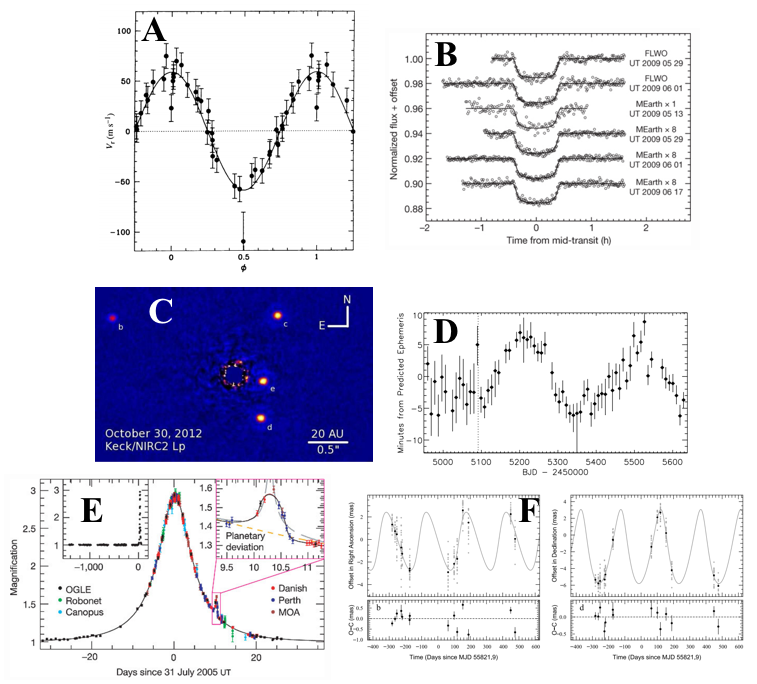
\includegraphics[width=\textwidth]{figures/detection_methods.png}
  \caption[Methods of exoplanet detection and characterization.]
      {Examples of observables for exoplanet detections using A)
    the radial velocity method \citep{mayor95}, B) planetary transits
    \citep{charbonneau09}, C) direct imaging \citep{currie14},
    D) transit timing variations \citep{ballard11},
    E) gravitational microlensing \citep{beaulieu06}, and
    F) astrometry \citep{sahlmann13}.}
  \label{fig:detection}
\end{figure}

\emph{Radial velocities}: the measurement of variations in the Doppler shift of star
around the barycenter of its planetary system due to the gravitational influence of
planetary-mass companions. This method is used to measure the planet-star orbital separation
and places a lower limit on the planet's mass. The radial velocity
method favours the detection of massive, short-period planets around inactive stars
(see Sect.~\ref{sect:rv} for more details). \\

\emph{Photometric transits}: monitoring the brightness of a star over time and
searching for periodically reoccurring brightness dips due to the occultation of the star
by an orbiting planet. This method is highly complementary to the radial velocity method
as it measures the planet's radius and orbital inclination where the latter can be
used to break the mass-inclination degeneracy suffered by radial velocity planet
detections. The recovery of radial velocity planet masses and planet radii from transit observations
together provide
views of planetary bulk densities that can be used to distinguish predominantly
rocky planets from planets with significant fractions of their sizes in gaseous envelopes.
The transit method is the most successful planet detection method as a single
wide-field camera can be used to monitor many stars simultaneously and continuously.
However, this method requires planets to have nearly edge-on orbits relative to the observer
and thus favours the detection of close-in giant planets orbiting small stars. \\

\emph{Direct imaging}: spatially resolving planets from their bright host stars and thus the
direct detection of photons originating from the planet. The resulting planetary luminosity
measurements can be compared to forward models of planetary
evolution to infer planet masses and possible formation pathways \citep{marley07}.
Multi-epoch observations can also reveal the nature of planetary orbits \citep{wang18}.
Due to the extremely small planet-star contrasts that are required to directly detect planetary 
companions, direct imaging favours the detection of young massive planets on wide orbits in the 
thermal infrared where the planet-star contrast is maximized. \\

\emph{Transit timing variations}: or TTVs, represent deviations in the expected transit
times of a transiting planet under the assumption of a linear ephemeris. Such deviations
may be attributed to an unseen planetary companion whose gravitational influence on the
transiting planet is observable either through close encounters or mean motion resonances.
The amplitude and periodicity of a transiting planet's TTVs can be used to constrain the mass
and orbital period of the perturbing planet although a mass-eccentricity degeneracy exists
for planet pairs close to mean motion resonances \citep{lithwick12}. \\

\emph{Gravitational microlensing}:
offers a unique method for probing the planet population out to large distances
within the Milky Way as the detected photons do not originate from the planetary system itself
but rather from a distant bright source. As the gravitational field of a
foreground star (i.e. the lens) occults a distant bright source, the source appears to
brighten as a result of the gravitational lensing effect. In the case for which the lens' gravitational
potential deviates significantly from radial symmetry because of a gravitational anomaly induced by a
planetary companion, that inhomogeneity in the gravitational field of the lens will disrupt the smoothness
of the field and cause an anomalous brightening that reveals the presence of a co-moving companion with
a measurable mass. One drawback of this method however is that observations of the same planetary
system are not repeatable due to the very precise alignment of the source and lens that is required. \\

\emph{Astrometry}: is similar to the radial velocity method wherein a planetary-mass companion
causes its host star to periodically wobble. The astrometry method is unique to the radial velocity
method as the observed variations occur in the plane of the sky in position space, rather than in velocity
space. This method is used to measure the orbital separation of a
star and planet and measure the planet's mass. Because the variation in the star's position
needs to be resolved, the astrometry method favours nearby planetary systems with massive
planets on wide-orbits. \\


\section{Exoplanet Detection via Stellar Radial Velocity} \label{sect:rv}
\subsection{Radial velocity curves}
The radial velocity (RV) method of detecting and characterizing exoplanets is largely
the focus of the work presented herein and so here I provide an overview of its formalism. \\

The RV method represents a simple 
application of Newton's third law: \emph{``for every action, there is an equal 
and opposite reaction''}. In this case, the presence of a planetary companion around a 
host star displaces the barycenter of that two-body system (i.e. the centre-of-mass) from the
centre of the star itself. Because of this, a star with a sole companion 
will execute a Keplerian orbit about the system's barycenter. The radial velocity of such a star
%as seen by any observer whose line of sight is not exactly orthogonal to the star's
%orbit normal,
is

\begin{equation}
V_r(t) = \gamma_0 + K[\cos{(\nu(t,P,T_0) + \omega)} + e\cos{\omega})],
\label{eq:rv}
\end{equation}

\noindent where $t$ is the independent time coordinate, $\gamma_0$ is the systemic velocity of
the star relative to the observer, $K$ is the semi-amplitude of the RV variation,
$P$ is the orbital period of the star and planet, 
$T_0$ is the reference epoch or time of inferior conjunction, and
the orbital elements $e$ and $\omega$ are the orbital eccentricity and argument of
periastron respectively. Note that $\omega$ is undefined for circular orbits with
$e=0$ and is assigned the conventional value of $\pi/2$ in such a scenario.
Eq.~\ref{eq:rv} is known as the Keplerian orbital solution.
The true anomaly 

\begin{equation}
\nu(t,P,T_0) = 2 \arctan{\left( \sqrt{\frac{1+e}{1-e}} \tan{\frac{E(t)}{2}}  \right)}
\end{equation}

\noindent defines the position of the star on its orbit 
relative to the argument of periastron and in the direction of motion. It is derived 
from another angular parameter, the eccentric anomaly $E(t)$. The eccentric 
anomaly can be solved for using the mean anomaly $M(t)$ according to 
Kepler's equation

\begin{equation}
M(t) = E(t)-e\sin{E(t)},
\label{eq:kepler} 
\end{equation}

\noindent where the mean anomaly is

\begin{equation}
M(t) = \frac{2\pi}{P} (t-\tau_{\mathrm{peri}}), 
\end{equation}

\noindent and $\tau_{\mathrm{peri}}$ is the epoch of 
pericenter passage. Because Eq.~\ref{eq:kepler} does not have a closed-form 
solution, in practice it is solved using iterative numerical techniques. 
Examples of Keplerian orbits using Eq.~\ref{eq:rv} are shown in Fig.~\ref{fig:rv} 
for two 5 Earth mass planets each with an orbital period of 2 days around a 0.2 M$_{\odot}$ 
star. The first planet is on a perfectly circular orbit and therefore induces a purely
sinusoidal RV variation on the host star while the second planet's eccentricity is 0.3 and
exhibits a RV variation that clearly differs from sinusoidal with the addition of the second
cosine term in Eq.~\ref{eq:rv}. \\

\begin{figure}
  \centering
  %\animategraphics[width=\textwidth,controls,loop]{200}{figures/RVcurve_}{0}{49}
  \caption[Animation of observed radial velocities for different orbital configurations.]
      {An animation of the orbits of two (non-interacting) planets of equal
    mass and on 2 day orbits around a 0.2 solar mass star. The first planet has a circular
    Keplerian orbit ($e=0$) while the orbit of the second exhibits some ellipticity with
    $e=0.3$. The lower panel depicts the corresponding RV variation induced on the host star
    by each planet independently.}
  \label{fig:rv}
\end{figure}

The Keplerian orbital solution is valid in the absence of dynamical 
perturbations to the two-body system. For Keplerian orbits, only the true anomaly in
Eq.~\ref{eq:rv} varies with time. However,
if additional bodies are present in the system such as in circumbinary  
systems or in high multiplicity planetary systems, then the parameters in 
Eq.~\ref{eq:rv} need not be fixed and we instead refer to the measured orbit as the 
osculating orbit that may vary between orbital cycles. Note that if the timescale 
for perturbations to the stellar orbital solution is comparable to or less than the 
time interval over which RV observations are obtained, then the Keplerian 
orbital solution is an insufficient description of the observations and one must consider
a more complicated treatment of the dynamics typically in the form of N-body simulations.


\subsection{Fundamental planet parameters from the radial velocity method} \label{sect:K}
If we consider the simplest planetary system containing a star and a planet, each body will 
orbit their common centre-of-mass (COM) whose position vector is

\begin{equation}
\mathbf{r}_{\mathrm{COM}} = \frac{M_s \mathbf{r}_s + m_p \mathbf{r}_p}{M_s + m_p},
\end{equation}

\noindent where $M_s$ and $m_p$ are the stellar and planetary masses respectively and
$\mathbf{r}_s$ and $\mathbf{r}_p$ are their position vectors. 
Let us now take a barycentric view of this two-body system such that the 
COM coordinate is located at the origin ($|\mathbf{r}_{\mathrm{COM}}|=0$). Further
assuming circular orbits (i.e. $e=0$) and working 
in absolute scalar terms, the orbital distances of the star and planet are  
related via 

\begin{equation}
a_s M_s = a_p m_p,
\label{eq:com}
\end{equation}
  
\noindent where we have written $|\mathbf{r}_s|=a_s$ and 
$|\mathbf{r}_p|=a_p$. For a circular orbit, the stellar velocity around the COM has
the constant value

\begin{equation}
v_s = \frac{2\pi a_s}{P}.
\label{eq:velocity}
\end{equation}

\noindent As the star orbits the COM the maximum observed radial velocity of the star
is realized when the magnitude of the star's radial velocity vector
equals its velocity $v_s$. At these points in the orbit, $V_r(t)=\text{max}(V_r(t))=v_s=K$.
Because the RV curve, and hence $K$, is observable, 
we can relate $K$ to the masses of the star and planet by combining the velocity 
equation (Eq.~\ref{eq:velocity}) with the COM equation (Eq.~\ref{eq:com})
and Kepler's third law:

\begin{align}
\mathrm{max}(V_r(t)) = K &= \frac{2\pi a_s}{P}, \\
&= \frac{2\pi}{P} \left( \frac{m_p}{M_s} \right) a_p, \\
&= \frac{2\pi}{P} \left( \frac{m_p}{M_s} \right) \left( \frac{GM_s}{4\pi^2} \right)^{1/3} P^{2/3}, \\
&= \left( \frac{2\pi G}{M_s^2 P} \right)^{1/3} m_p. \label{eq:K1}
\end{align}

Eq.~\ref{eq:K1} contains two quantities that are directly observable from the RV time series.
Namely, the orbital period $P$ and semi-amplitude $K$. Observers will often seek an independent
constraint on the stellar mass $M_s$ from say the comparison of the stellar spectrum to
spectral templates of known stellar mass from stellar evolution models
\citep[e.g.][]{muirhead12} or from
empirical relations between optical or near-IR stellar luminosities and dynamically
measured stellar masses \citep[e.g.][]{benedict16,mann19}. Prior knowledge of the
stellar mass enables the mass of the planetary companion to be inferred from RV time series
using Eq.~\ref{eq:K1}.
The uncertainties in the resulting planet mass 
measurement are typically dominated by the noise in the dataset which directly affects the
measurement precision of $P$ and $K$. Additional uncertainties in $m_p$ are also introduced by
the uncertainty in $M_s$ which motivates the need to develop a detailed understanding of
fundamental stellar parameters to enable precise exoplanet measurements. \\

Looking more closely at Eq.~\ref{eq:K1} we can see that the RV semi-amplitude scales 
linearly with planet mass but has a negative scaling with stellar mass and orbital 
period. This makes sense because the RV effect is a manifestation of a gravitational effect.
An increased perturbing mass (i.e. $m_p$) will result in an increased perturbation to the 
central body which itself becomes more difficult to perturb if more massive. Also, the 
effect weakens as the distance between the two bodies is increased (i.e. larger $P$). The 
RV method therefore has a natural observational bias towards massive, 
close-in planets around low mass stars as the combination of these parameters will maximize the
RV signal and increase the chances of that signal being detected above the noise (see
Sect.~\ref{sect:error}). This explains why the first planets to be detected with the
RV method were hot Jupiters \citep[e.g.][]{mayor95}.
%For reference, the RV semi-amplitude that the Earth 
%induces on the Sun is $\sim 9$ cm s$^{-1}$ whereas the $\sim 300$ times more massive Jupiter
%induces a $\sim 12$ \mps{} effect despite having a factor of $\sim 5$ wider orbit.

\subsection{Caveats to Eq.~\ref{eq:K1}}
In the derivation of the RV semi-amplitude (Eq.~\ref{eq:K1}) we have neglected two 
important geometric effects. The first is that of eccentricity which, if non-zero, 
causes the stellar velocity to vary throughout its orbit such that
$\text{d}v_s/\text{d}t \ne 0$. Instead $\mathrm{max}(V_r(t)) > 2\pi a_s/P$ 
because the conservation of angular momentum requires that $v_s(\tau_{\text{peri}})$ 
be greater than elsewhere on the orbit. The corresponding correction 
factor to Eq.~\ref{eq:K1} is $(1-e^2)^{-1/2}$. \\

The second effect is that of inclination. When attempting to measure the planetary 
mass from RVs the orbital inclination of the planetary orbit\footnote{Orbital 
inclination is conventionally measured  relative 
to the plane of the sky; i.e. an edge-on orbit has $i=90^{\circ}$.} is degenerate with
$m_p$ and is entirely unknown unless the planet has an a-priori measurement of its orbital
inclination from either transit or astrometric observations. But the majority of planets are
neither transiting nor induce a resolvable astrometric variation and thus have unknown
orbital inclinations. For these planets, RV measurements 
are only sensitive to a mass lower limit $m_p\sin{i}$ rather than to the absolute planet mass.
The $\sin{i}$ correction factor also illustrates that an RV signal is only non-zero when
the observer's orientation is not exactly orthogonal to the normal of the star's orbital plane;
i.e. face-on orientations with $i=0$. \\

The inclusion of these correction factors gives a more complete description of the RV semi-amplitude
compared to Eq.~\ref{eq:K1}: 

\begin{equation}
K = \left( \frac{2\pi G}{M_s^2 P} \right)^{1/3} \frac{m_p \sin{i}}{\sqrt{1-e^2}}. 
\label{eq:K2}
\end{equation}

\section{Measuring Radial Velocities} \label{sect:spectrograph}
\subsection{Stellar Spectroscopy}
Radial velocity variations induced by planetary companions cause the star to become 
periodically Doppler shifted. These wavelength shifts can be detected using high resolution 
spectroscopy as spectral features originating from the stellar photosphere are shifted from
their rest wavelength $\lambda_{\text{rest}}$ as the star's velocity changes along the
line-of-sight according to 

\begin{equation}
\frac{\Delta \lambda}{\lambda_{\text{rest}}} = \frac{V_r}{c},
\end{equation}

\noindent where $\Delta \lambda = \lambda_{\text{obs}}-\lambda_{\text{rest}}$ and
$\lambda_{\text{obs}}$ is the observed wavelength of the spectral features. 
In practice, RV shifts are often measured from the cross-correlation of 
the observed stellar spectrum with a master empirical spectrum or template mask
that is shifted in velocity space to map their correlation over relative velocities
\citep{astudillodefru15}. The resulting RV precision is enhanced when the individual velocities
of many lines can be averaged. This makes precision RV measurements especially tractable for M
dwarfs as they exhibit a plethora of 
spectral lines that become more abundant towards later type stars.
A sample of infrared spectra of early-to-late M dwarfs 
are shown in Fig.~\ref{fig:spectra} to demonstrate their wealth of absorption features
\citep{rayner09}.  \\

\begin{figure}
\centering
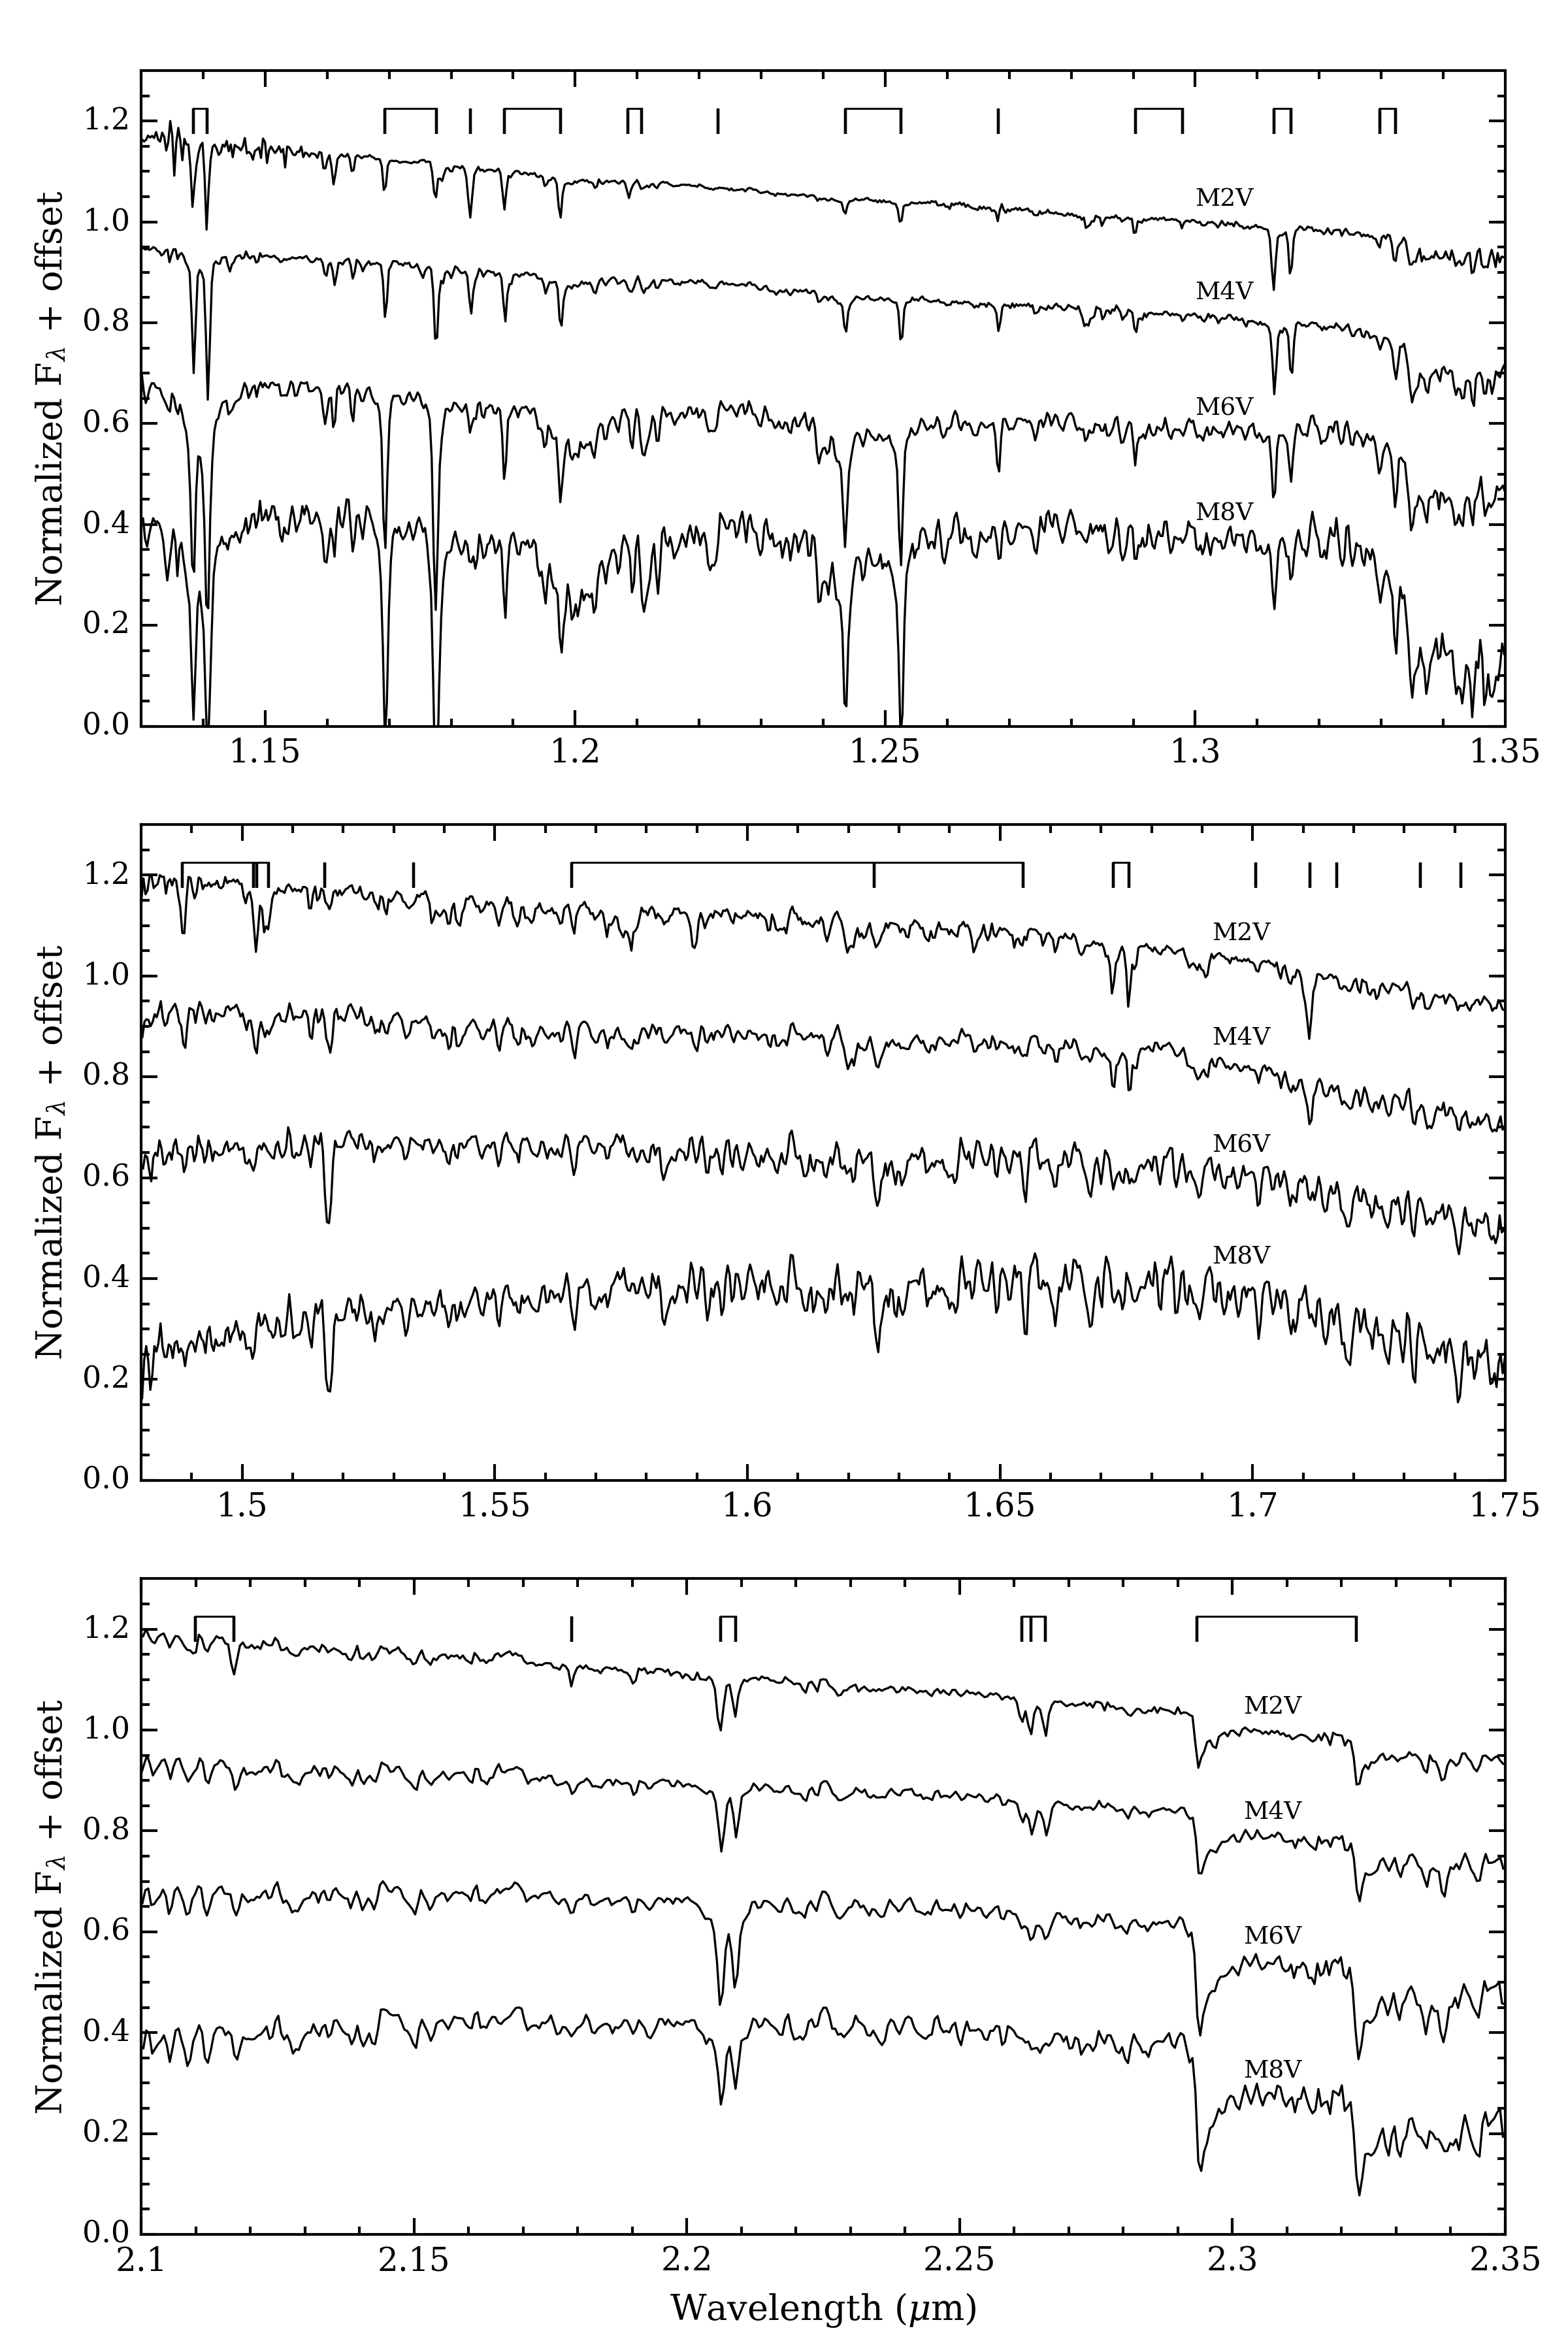
\includegraphics[width=0.8\hsize]{figures/Mdwarf_spectra.png}
\caption[Near-IR spectra of early-to-late M dwarfs.]
        {Medium resolution spectra ($R=\lambda / \Delta \lambda \sim 2000$)
          for four early-to-late M dwarfs in the J band (\emph{top}),
  H band (\emph{middle}), and K$_{\text{S}}$ band (\emph{bottom}) from the SpeX spectrograph
  at NASA's Infrared Telescope Facility. \label{fig:spectra}}
\end{figure}

The aforementioned
spectroscopic measurements are made using a stabilized spectrograph at high spectral resolution
($R=\lambda / \Delta \lambda$) that contains a grating to 
diffract or spatially disperse the incoming source light into its various colour components.
Echelle spectrographs in particular include an additional high order grating that separates the
light into spectral orders that are subsequently cross-dispersed spatially onto the detector. The
dispersed spectral orders create the observed stellar spectrum (Fig.~\ref{fig:harps}).
After 1D spectral extraction, the spectrum is cross-correlated with the aforementioned master spectrum
or template mask wherein prominent lines 
are averaged to create the cross-correlation function (CCF) of the star at the epoch of 
observation. Traditionally, the CCF is typically fit with a Gaussian line profile whose best-fit mean 
is equal to the measured radial velocity \citep{pepe02}. It should be noted however that the net
convective blueshift in stellar photospheres causes the native CCF to be asymmetric rather
than purely Gaussian even in the absence of surface inhomogeneities \citep{gray89}.
Active regions on the stellar surface arising 
from the presence of magnetic fields can have additional effects on the observed CCF 
causing the line profile to exhibit additional and localized non-Gaussianities. 
These distortions can in principle be used to model stellar activity in cases for which the distortions
can be detected at high signal-to-noise and their origin dominates the astrophysical RV budget (as opposed
to being due to systematic effects). \\

\begin{figure}
  \centering
  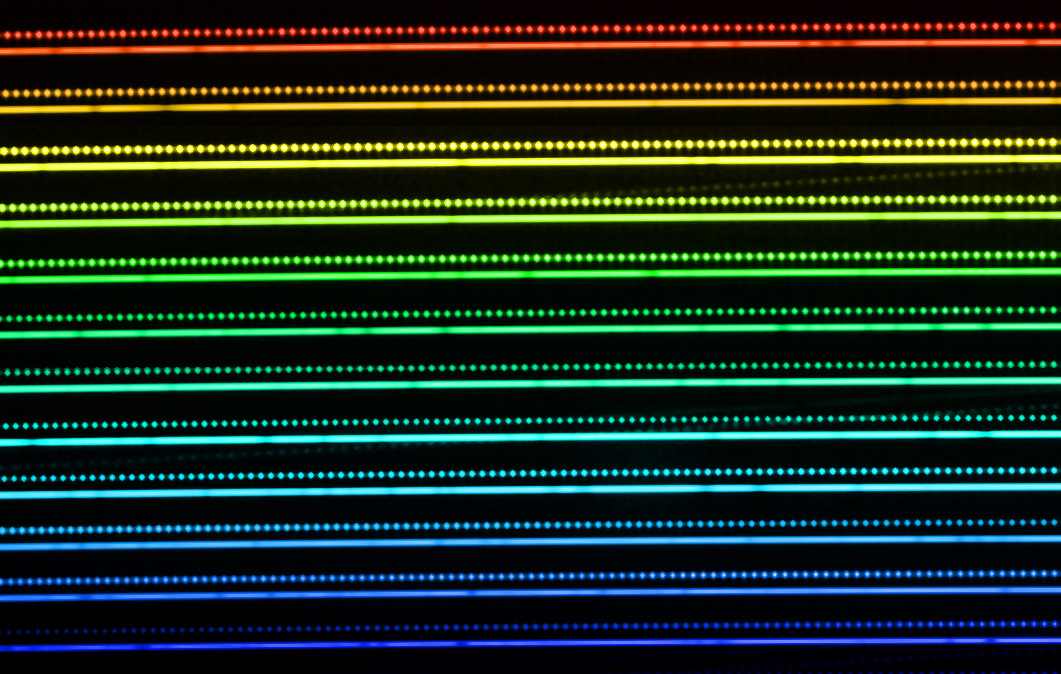
\includegraphics[width=0.8\hsize]{figures/20140904_harps-lasercomb.jpg}
  \caption[Image of spectral orders from the HARPS echelle spectrograph.]
      {A colourized image of the HARPS detector showing a subset of its 72 spectral orders.
    Each row pair contains the stellar spectrum (solid spectrum) over a portion of the HARPS wavelength
    domain and the corresponding wavelength reference from its laser frequency comb (dotted spectrum).
    Accurate wavelength calibration enables monitoring of stellar absorption features over time that
    may reveal periodic Doppler shifts possibly indicative of a planetary companion.
    Image credit: \emph{European Southern Observatory}.}
  \label{fig:harps}
\end{figure}


\subsection{Radial Velocity Error Budget Overview} \label{sect:error}
The complete error budget when conducting precision RV measurements features many contributing factors.
Among these are instrument/facility limitations, the fundamental photon noise limit, imperfect corrections
of telluric contamination, and astrophysical noise. Here we review the RV error budget
with a particular focus on stellar activity as it pertains to the work presented in this thesis.

\subsubsection{Instrumentation Challenges}
RV spectrographs have an inherent RV precision that is set by a multitude of individual error sources
that hinder a user's ability to measure infinitesimally precise
RVs \citep{podgorski14,halverson16}.
These issues are intrinsic to the experimental hardware and their relative contributions
vary significantly between instruments with often not a single source of error dominating the instrumental
error budget. \\

A non-exhaustive list of prominent issues with RV spectrographs includes 

\begin{multicols}{2}
  \begin{itemize}
  \item thermal stability,
  \item pressure stability,
  \item wavelength calibration,
  \item vibration control,
  \item drift control,
  \item detector imperfections (i.e. readout noise, intrapixel quantum efficiencies, etc),
  \item internal scattered light,
  \item fibre modal noise,
  \item tracking errors,
  \item focus errors,
  \item etc.
  \end{itemize}
\end{multicols}
  
\noindent The aforementioned RV error sources arise from the design and operation of the
instrument and telescope facility. As such, their mitigation is set by the hardware specifications
and cannot be significantly improved by post processing. These challenges associated with building
state-of-the-art RV instrumentation are not the focus of
this thesis but it is important to note their contributions to the overall RV error budget as together
they set a limit to the highest possible RV precision attainable with a given instrument.

\subsubsection{Photon noise limit}
The photon noise limit represents the fundamental limit to the RV measurement precision that can
be obtained from a stellar spectrum $A_i$ where $i$ is the index over wavelength elements.
The photon noise limited RV precision from \cite{bouchy01} is

\begin{equation}
  \sigma_{\gamma} = \frac{c}{\text{S/N} \cdot Q}
\end{equation}

\noindent where $c$ is the speed of light, S/N is the signal-to-noise of the spectrum over its
complete spectral domain, and

\begin{equation}
  Q = \frac{\sqrt{\sum_i W_i}}{\sqrt{\sum_i A_i}}
\end{equation}

\noindent is known as the quality factor and represents the density of RV information content
in the spectrum $A_i$ measured in photoelectrons. The weighting function is given by

\begin{equation}
  W_i = \left( \frac{\lambda_i^2}{A_i} \right) \left( \frac{\partial A_i}{\partial \lambda_i} \right)^2.
  \label{eq:weight}
\end{equation}

By the dependence of $\sigma_{\gamma}$ on the first spectral derivative of the observed spectrum
(Eq.~\ref{eq:weight}), it is clear that
high S/N spectra with a high density of sharp features provide the
best possible RV precision. Because the sharpness of the lines is important, obtaining high
resolution spectra has a direct benefit on minimizing $\sigma_{\gamma}$. Similarly, stars
with low levels of collisional and rotational broadening (i.e. low $\log{g}$ and \vsini{)} are
favourable targets for minimizing $\sigma_{\gamma}$. Also because line density is important, cooler stars
or stars with a high metallicity are favourable as they exhibit more molecular and metal features over which
counting errors can be minimized. Fig.~\ref{fig:sigrv} demonstrates these dependencies over the spectral
bands $UBVRIYJHK_{\text{S}}$.

\begin{figure}
  \centering
  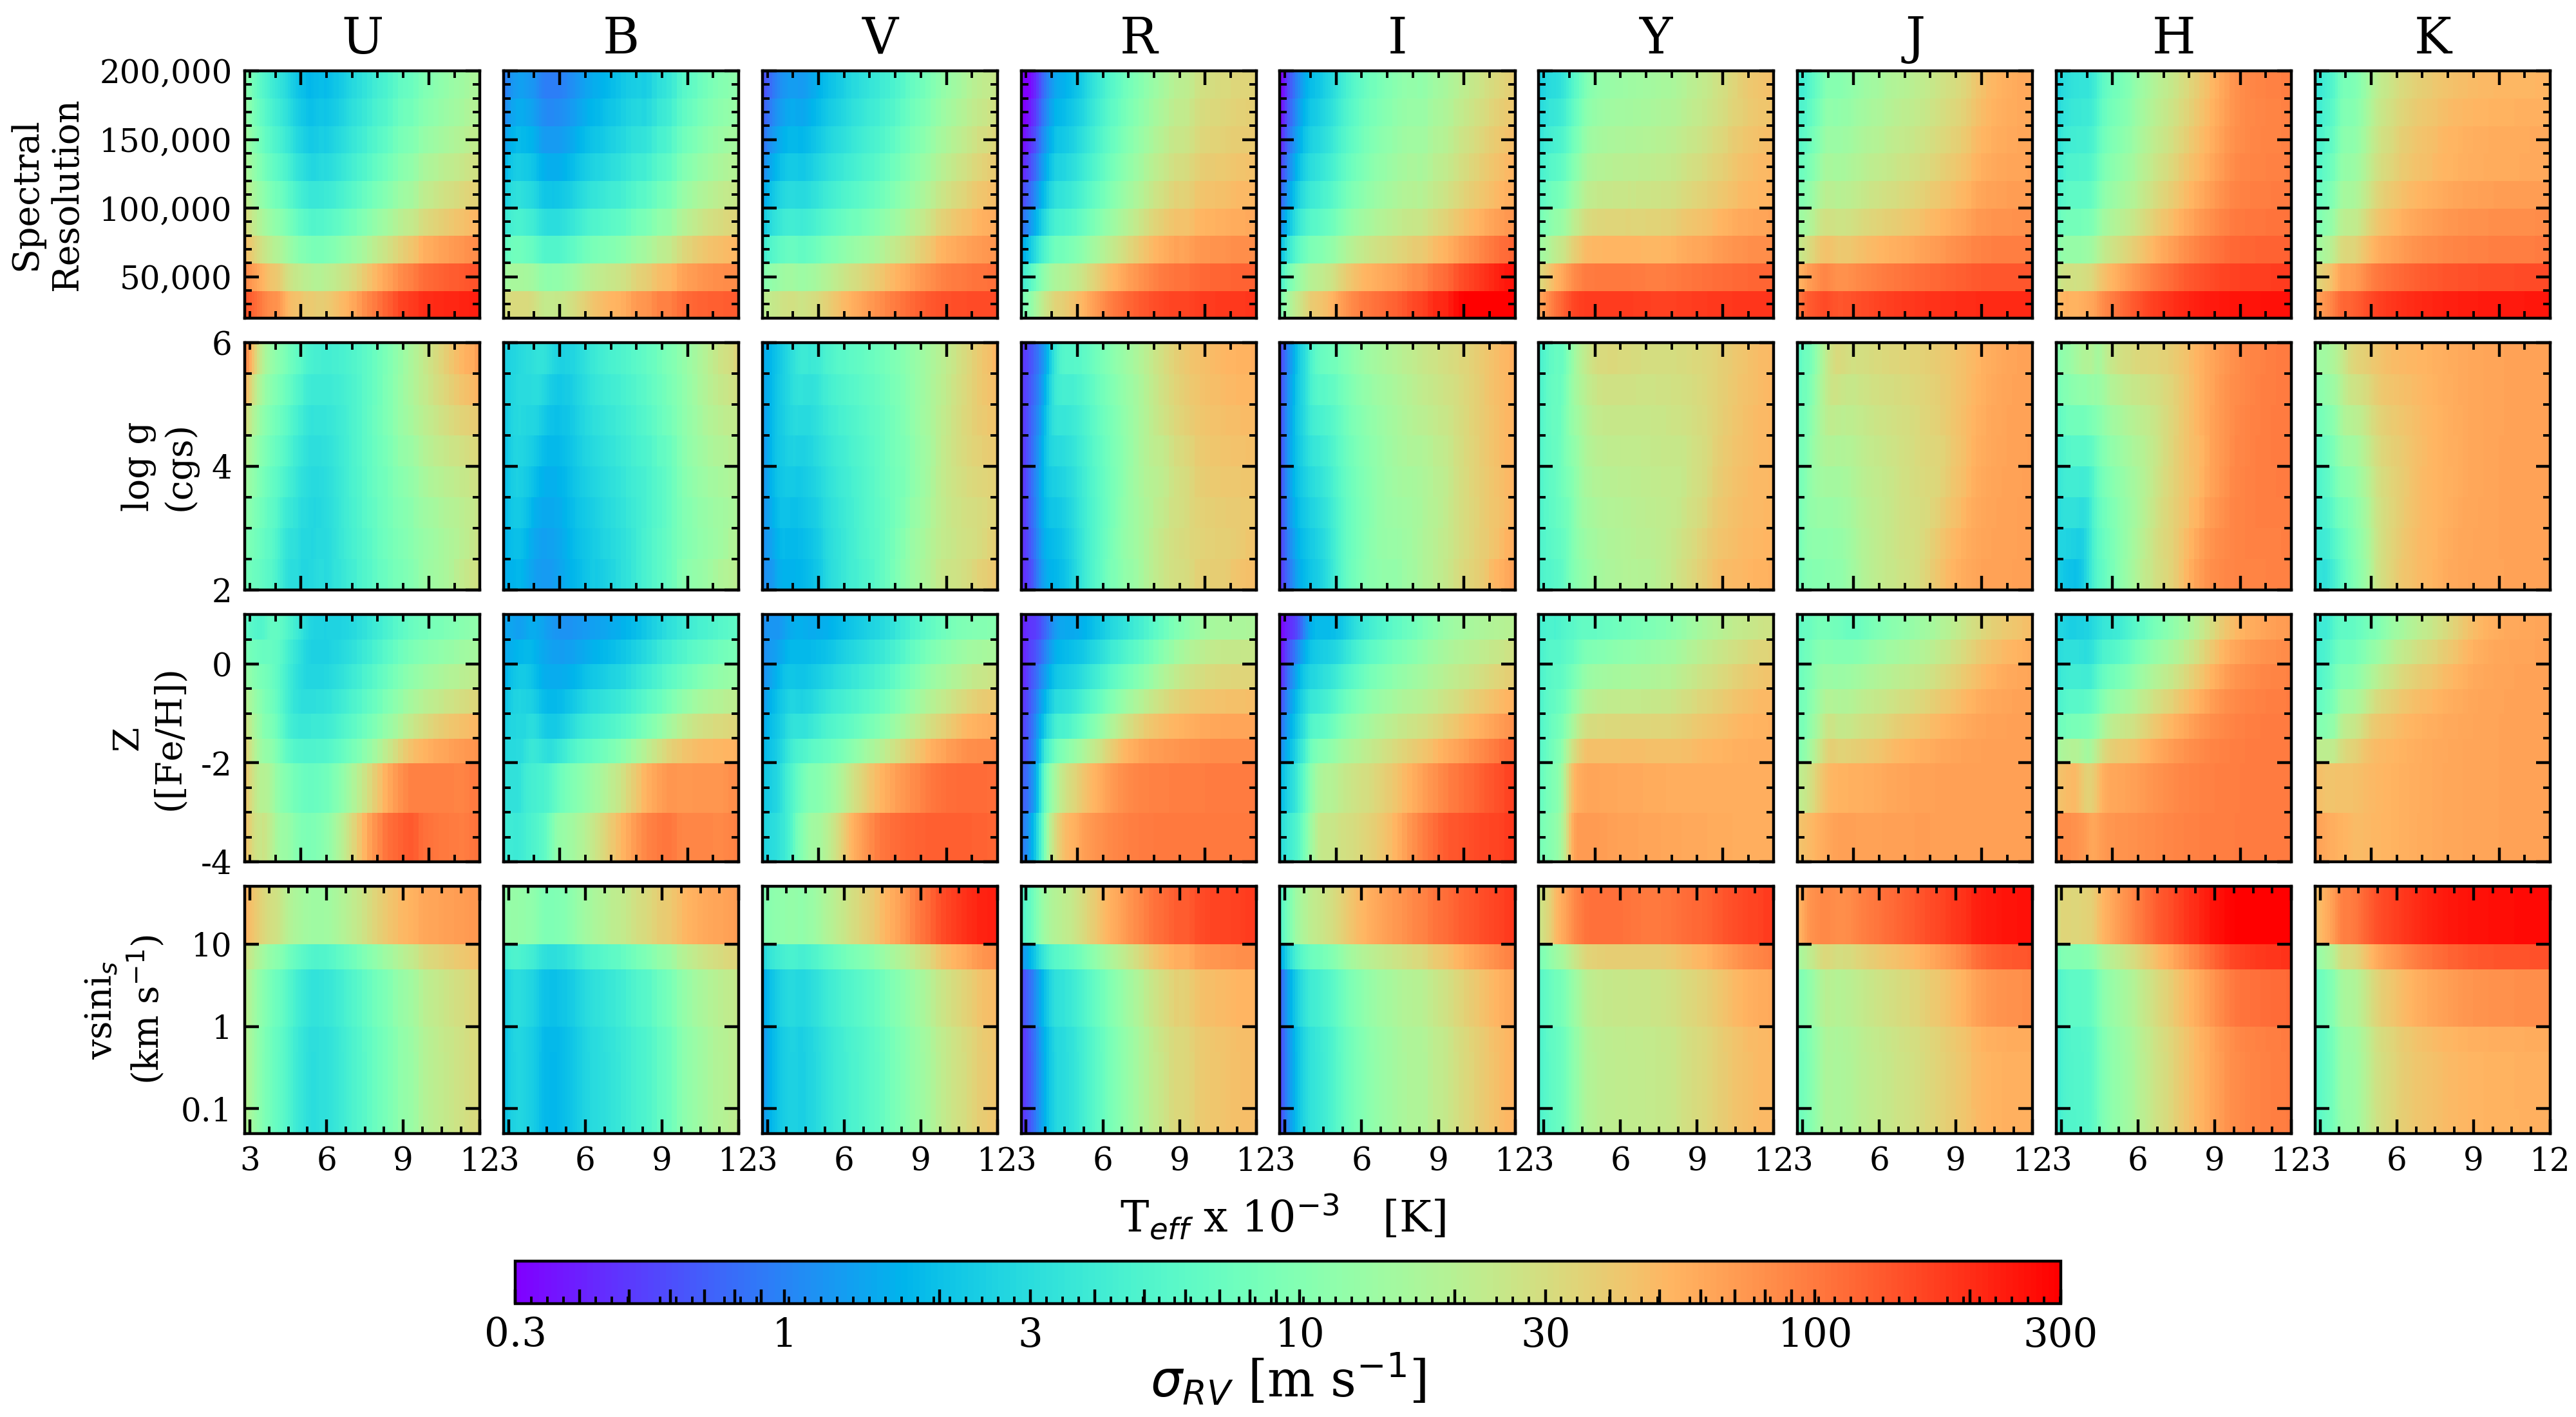
\includegraphics[width=\textwidth]{figures/sigRV_grid.png}
  \caption[Doppler information content over spectral band passes and stellar properties.]
      {Distributions of the photon noise limited RV precision in the $UBVRIYJHK_{\text{S}}$
    bands and as a function of spectral resolution, $\log{g}$, metallicity, \vsini{,}
    and stellar effective temperature. The distribution shown in each subpanel is marginalized
    over all parameters not depicted on either of the panel's axes and is therefore not
    representative of true $\sigma_{\gamma}$ values particularly in the near-IR bands
    in which telluric contamination is not properly treated.}
  \label{fig:sigrv}
\end{figure}

\subsubsection{Telluric contamination} \label{sect:tellurics}
In addition to error floors arising from the instrumentation and the photon noise limit,
other physical sources of RV errors exist that need to be accounted for in the post-processing
software. One example is the effect
of telluric contamination of the stellar spectrum by spectral features originating from Earth's
atmosphere. Because all high precision RV experiments to date are executed from the ground
the incoming starlight must traverse much of the Earth's atmosphere at which time telluric
absorption and emission features become
imprinted on the incident spectrum. This effect is much more prominent in the infrared where
the atmosphere becomes more opaque over wider spectral bands than in the visible due
in large part to absorption bands by various greenhouse gases such as H$_2$O
(Fig.~\ref{fig:transmission}). In the visible, small regions
in wavelength space that are known to be contaminated by tellurics can be simply masked without
significant loss of RV content. Whereas this method if applied to near-IR spectrographs 
eliminates such a large fraction of the available RV information that it effectively negates the
benefits of developing near-IR RV spectrographs at all.
Instead, near-IR RVs must rely on more sophisticated methods of telluric spectrum extraction and
removal based on atmospheric transmission models \citep[e.g.][]{vacca03,bertaux14}
and/or data-driven methods \citep[e.g.][]{artigau14,bedell19}.

\begin{figure}
  \centering
  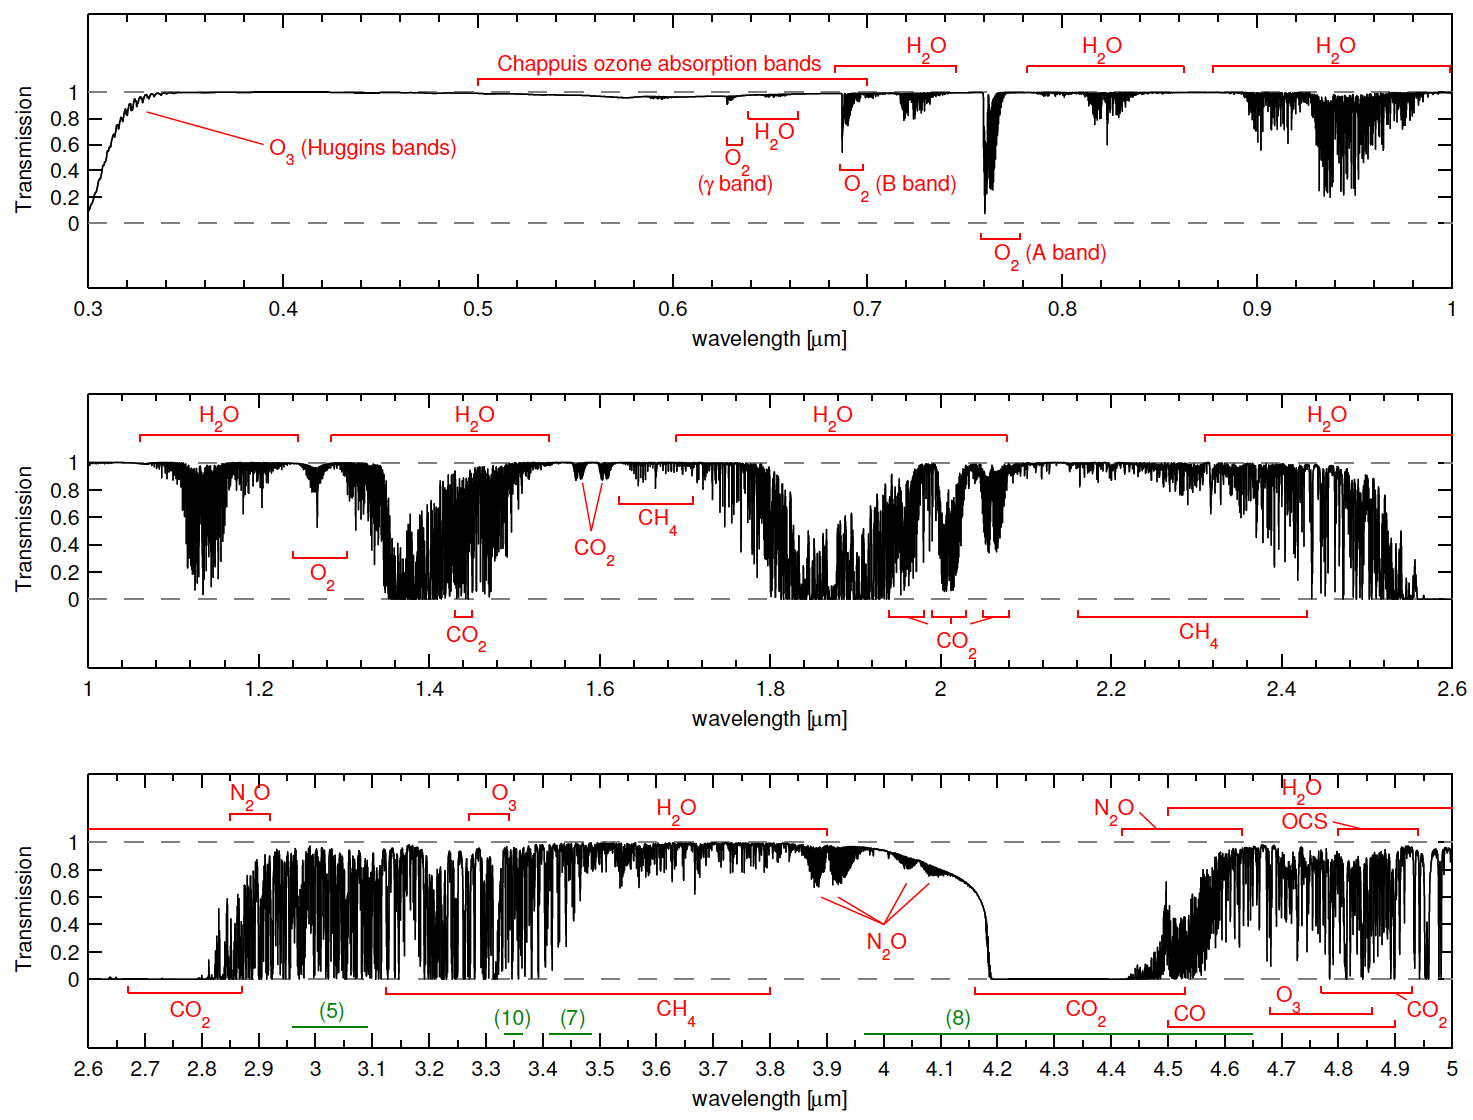
\includegraphics[width=0.8\hsize]{figures/transmittancev2.png}
  \caption[Atmospheric transmission from 0.3-5 $\mu$m.]
          {A model of telluric absorption from 0.3-5 \micron{} calculated using the LBLRTM radiative transfer
            code \citep{clough05}. The atmosphere becomes increasingly opaque towards infrared wavelengths with
            narrow observing windows at the $YJHK_{\text{S}}LL'$ bands. Telluric absorption in the optical is
            dominated by O$_2$, O$_3$, and H$_2$O while the near-IR wavelengths feature strong H$_2$O absorption
            bands in addition to other strong absorbers such as CO, CO$_2$, CH$_4$, OCS, and N$_2$O.
            \citep[Image credit:][]{smette15}}
  %\caption{A \texttt{TAPAS} model of the radiative transmittance through the Earth's atmosphere
  %  as seen from MaunaKea at an airmass of unity \citep{bertaux14}. It is clear that the atmosphere
  %  becomes increasingly opaque towards infrared wavelengths with small observing windows at the
  %  $YJHK_{\text{S}}$ bands.}
  \label{fig:transmission}
\end{figure}

\subsubsection{Stellar activity} \label{sect:activity}
There exists a variety of physical processes in the photospheres and chromospheres of stars that
can lead to temporally correlated RV signals that are collectively
referred to as \emph{stellar activity}. Alternatively, activity sources that act on short timescales
(i.e. seconds to minutes) and are unrelated to magnetic processes are sometimes referred to as stellar jitter.
Particularly in RV planet studies, stellar activity
signals are the bane of observers searching for sub-Neptune-sized planets because activity signals
can mask and in certain instances even mimic the typically small planetary signals of interest. \\

Depending on the exact physical process these
signals can have widely differing timescales and manifestations in
spectroscopic, photometric, and polarimetry observations. Activity
signals from active regions such as cool star spots and chromospheric plages 
are also wavelength dependent unlike Doppler variations induced by
planetary companions \citep{tal-or18}. Ancillary time series to RV measurements
derived from any of the aforementioned observations may therefore be used to
disentangle stellar activity from achromatic Doppler shifts induced by a companion.
Such observables include spectroscopic activity indicators such as the $H\alpha$ and
\caii{} H \& K indices that are magnetically sensitive features originating from the hot stellar
chromosphere, line deformation diagnostics (e.g. CCF shape parameters; \citealt{boisse11},
line-by-line analyses \citealt{davis17,dumusque18}), plus Doppler imaging of the stellar surface
\citep{hebrard16} (see Sect.~\ref{sect:indicators} for details). \\

Examples of sources of stellar activity are summarized below
while a brief overview is given in Table~\ref{table:activity}. \\

\begin{table*}
\small
\renewcommand{\arraystretch}{0.7}
\caption[]{Summary of Radial Velocity Stellar Activity Sources}
\label{table:activity}
\begin{tabular}{cccl}
  \hline \\ [-1ex]
  \textbf{Activity} & \textbf{Typical} & \textbf{Typical Signal} & \textbf{Notes} \\
  \textbf{Source} & \textbf{Timescale} & \textbf{Amplitude} & \\
  \hline
  Flares & a few minutes & tens of \mps{} & Has distinct photometric and spectroscopic signatures. \\ 
  &&&Observations during a flaring event should be excluded \\
  &&& from planet searches$^1$. \\
  \hline
  Oscillations & tens of minutes & few \mps{} & Can be mitigated with sufficiently long exposure times \\
  &&&or multiple observations per night$^2$. \\
  \hline
  Granulation & tens of minutes & few \mps{} & See oscillations.  \\
  \hline
  Active Regions & few stellar & sub-\mps{} $\to$ & Timescale and amplitude depend heavily on the active \\
  & rotation periods & tens of \mps{} & region sizes and on stellar rotaton$^3$. See Fig.~\ref{fig:rotation} for \\
  &&& the distribution of M dwarf \prot{.} \\
  \hline
  Magnetic Cycles & $\sim  7-30$ years & tens of \mps{} & Is only important when searching for \\
  &&&long period planets.
  \end{tabular}
\begin{list}{}{}
\item {\bf{Notes.}}
      $^{1}$ \cite{reiners09}, $^2$ \cite{dumusque11a}, $^3$ \cite{dumusque11b}. \\
\end{list}
\end{table*}


\emph{Flares}: magnetically active stars can undergo energetic flares or coronal mass
ejections originating from the stellar atmosphere. The exact flare physics
in M dwarfs remains uncertain but clearly requires strong magnetic fields
that can be sustained by turbulent convective motions and rotation
\citep{browning08}. Flare events are easily identifiable as they
exhibit a characteristically rapid increase in brightness (or in the intensity
of certain emission lines; e.g. Ca II, He I, H$\alpha$, etc. \citealt{schmidt12})
followed by an exponential decay over hours. Because RV
measurements affected by flares can be easily identified by the characteristic
line intensity spike over short timescales, such measurements are commonly
removed from planet searches \citep{reiners09}. \\

\emph{Stellar Oscillations}:
small scale mechanical perturbations to the internal stellar structure
can give rise to oscillation modes. If not damped, these oscillations
can propagate through the stellar interior before rebounding at the surface
of the star thus creating observable pulses in brightness and in the RVs at a
few \mps{} and on timescales of a few to tens of minutes \citep{bedding01}. 
This phenomenon is predominantly observed in Sun-like and post main sequence stars.
Due to the short timescale of
pulsation variations in RV measurements of pulsating stars, the corresponding
jitter is often mitigated with sufficiently long exposure times
\citep{lovis05, dumusque11a}. \\


\emph{Granulation}:
stars with outer convection zones like the Sun and M dwarfs exhibit granulation patterns
at their surfaces. The granulation pattern is the result
of convection cells penetrating the surface; hot fluid parcels rising to the surface before
cooling and descending back into the stellar interior (see Fig.~\ref{fig:granulation}).
These patches of hot rising fluid are therefore brighter than the surrounding regions of cold
descending fluid. Furthermore, the relative fractional coverage of a star's surface by rising
fluid parcels is in general greater than that of descending ones as evidenced in
Fig.~\ref{fig:granulation}.
Along the line-of-sight, the RV component of photons emitted by the rising parcels at the
photospheric boundary will be blueshifted whereas the receding fluid within the
`intergranular lanes' will be redshifted. The domination of the stellar
surface area by hot parcels results in a granulated star having a net \emph{convective
  blueshift} that in turn creates an asymmetry in the disk-integrated spectral line profile
with additional power at blueshifted velocities. The effect of granulation is also known
to decrease towards cool M dwarf stars \citep{dumusque11a,meunier17}. \\

\begin{figure}
  \centering
  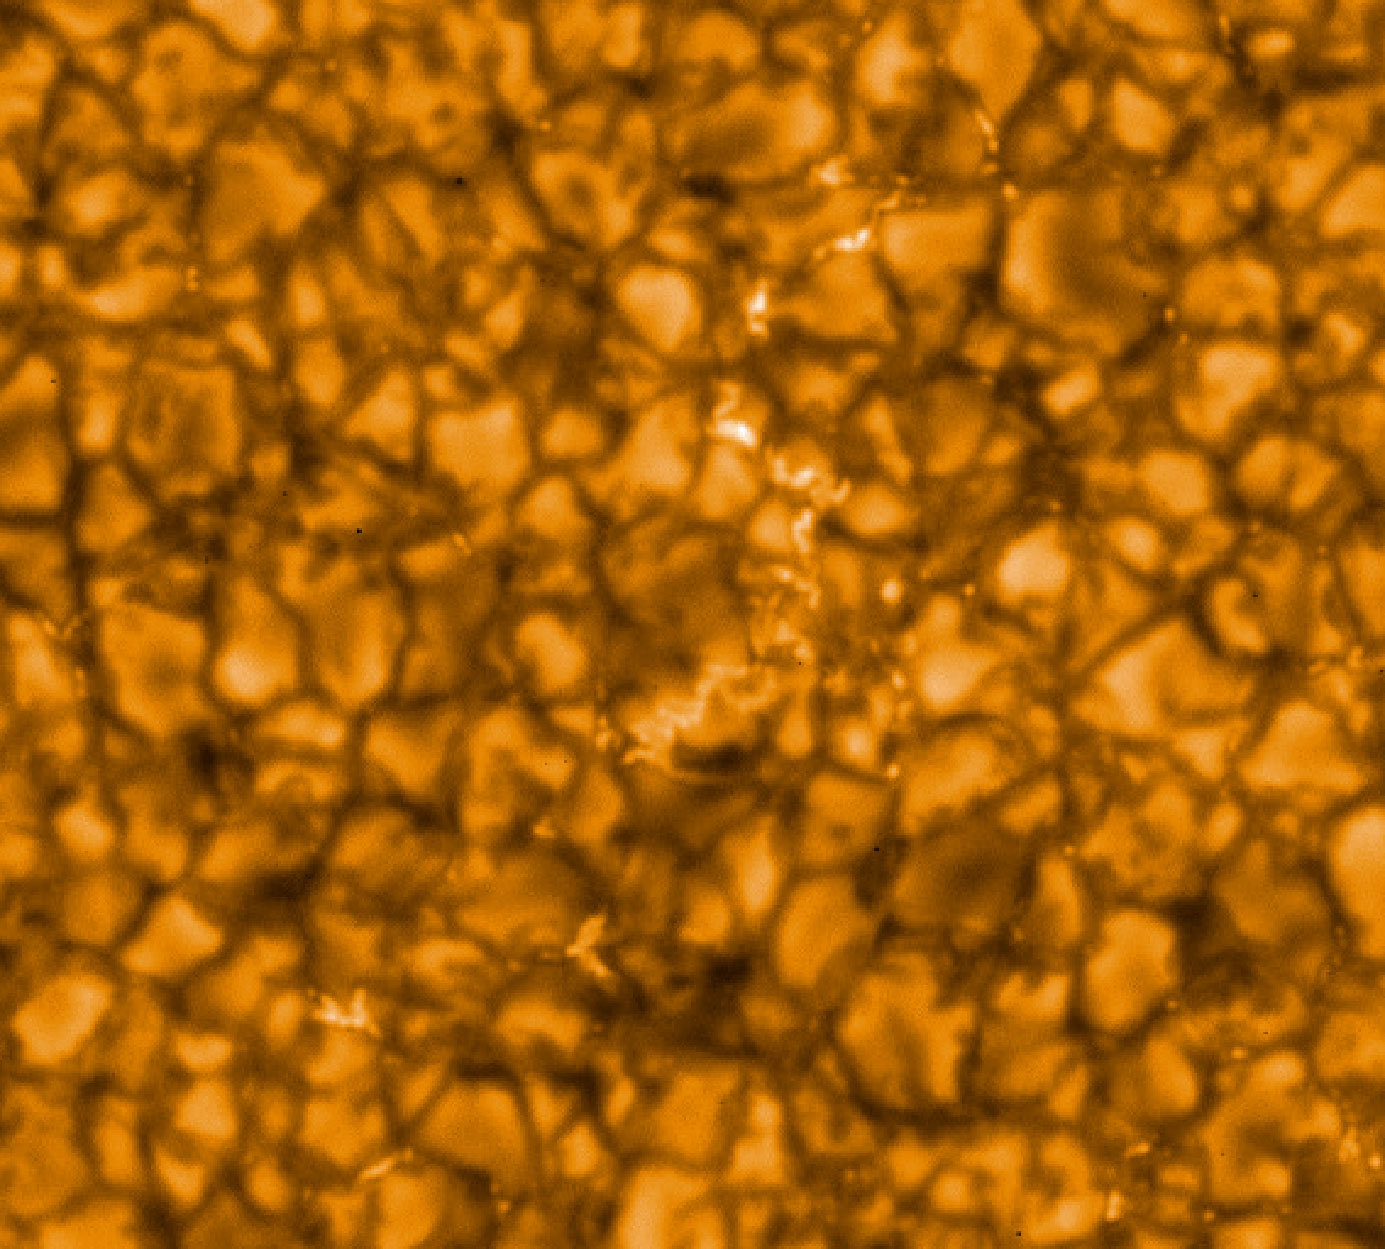
\includegraphics[width=0.7\textwidth]{figures/solargranulation.jpg}
  \caption[Close-in view of the convection cells on the solar surface.]
      {An image of a patch of the solar surface taken with NASA's Hinode Optical
    Telescope. The bright regions are the result of rising hot fluid parcels whereas the cooler,
    `intergranular lanes' reveal where the gas has cooled and descends back into the solar
    interior. (Image credit: Hinode JAXA/NASA/PPARC)}
  \label{fig:granulation}
\end{figure}


The short lifetimes of typical granules
\citep[$\sim 10$ minutes;][]{hall08,gilliland11} implies that brightness variability of the
surface varies on a similar timescale. However, `supergranules' may also persist over longer
timescales albeit with smaller RV contributions \citep[$\lesssim 1$ \mps{;}][]{rincon17}
%Such variations have been measured using high cadence photometry
%\citep[e.g.][]{gilliland11}.
The corresponding RV jitter is dependent on the time variability of the relative velocity of 
convective cells across the stellar surface. 
Noting that the relative sizes of granules varies over time, so
too does the resulting RV jitter whose net effect (hot and cold regions partially
cancel each other) is typically at the level of a few \mps{} \citep{lindegren03}. \\

\emph{Active Regions}:
like the Sun, the photospheres of active M dwarfs are littered with active regions such
as dark photospheric starspots, hot faculae, or plages in the chromosphere. Indeed,
the activity signals from active regions appear to dominate the RV activity budget on M dwarfs
\citep{lindegren03}. These localized regions of either
hot or cold gas relative to the surrounding photosphere become trapped by magnetic field loops reconnecting
with the stellar surface. Active regions create a temporally evolving
RV signal and spectral line profile distortion due to their distinct emitting temperatures and their orientation
as they rotate in and out of view (see Fig.~\ref{fig:starspot}). In the Sun, these structures
have long been known to be associated with strong local magnetic fields as evidenced by the observed
Zeeman splitting of lines emitted from these active regions \citep{hale08}. \\

\begin{figure}
  \centering
  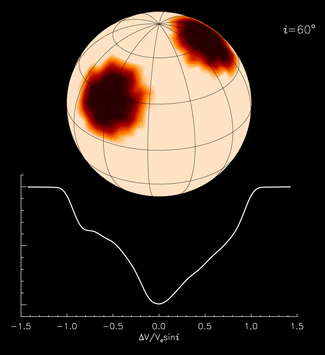
\includegraphics[scale=.8]{figures/starspot.png}
  \caption[Illustration of the effect of active regions on the integrated stellar line profile.]
      {An snapshot example of a spotted stellar photosphere and its effect on the disk-integrated
    spectral line profile. The cool spots depicted here disrupt the symmetry of the
    line profile according to the temperature difference between the spot and
    unspotted photosphere at its position on the stellar disk.
    \citep[Image credit:][]{kochukhov16}}
  \label{fig:starspot}
\end{figure}

The activity timescale from active regions is modulated by the stellar rotation. The stellar rotation
period \prot{} can often be measured for active stars with non-zero
inclination from the quasi-periodicity of their photometric variability.
The spectroscopic method of measuring a star's rotation state is done by measuring the projected
stellar rotation velocity \vsini{\footnote{Slowly rotating stars with correspondingly small \vsini{}
    values may not be detectable with insufficient spectral resolution. In such cases, only an upper
    limit on \vsini{} can be measured.}} via the rotational broadening
of its spectral features \citep{gray08}.
Because active regions are associated with magnetic activity and stellar
magnetic fields require rotation in order to be sustained over long timescales, rapidly rotating
late-type stars tend to be more magnetically active.
Fig.~\ref{fig:activity} demonstrates that the fraction of active M dwarfs is sustained at slower
rotation states in later M dwarfs than in early M dwarfs and that the activity fraction in general 
decreases as the stars spin-down via magnetized braking from stellar winds
\citep{skumanich72}. A measure of stellar rotation can therefore be used as a first-order
indicator of a star's activity level. \\

\begin{figure}
  \centering
  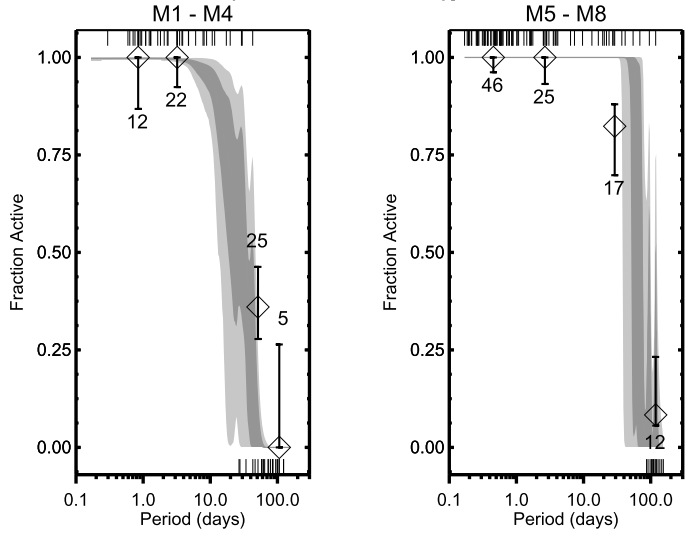
\includegraphics[width=.8\textwidth]{figures/mdwarfactivity.png}
  \caption[M dwarf activity fraction versus spectral type and stellar rotation.]
      {The fraction of active M dwarfs as a function of stellar rotation period
    for early-to-mid (\emph{left panel}) and mid-to-late (\emph{right panel}) M
    dwarfs. An individual star's activity flag is based on the ratio of its H$\alpha$ emission
    luminosity to its bolometric luminosity.
    The activity fraction of stars is seen to decrease as rotation slows although mid-to-late M
    dwarfs can maintain a higher activity fraction than early-to-mid M dwarfs within a given
    \prot{} bin. \citep[Image credit:][]{west15}}
  \label{fig:activity}
\end{figure}

Fig.~\ref{fig:rotation} depicts the rotation period
distribution of M dwarfs in the solar neighbourhood \citep{newton16a} and in the Kepler
field up to \prot{} $< 70$ days \citep{mcquillan13a}.
Two distinct populations exist, namely a rapidly
rotating population (\prot{} $\lesssim 3$ days) and a slowly rotating population
(\prot{} $\gtrsim 50$ days). It has been proposed that these two populations
have a distinct range of ages with
the slow rotators belonging to an older stellar population based on their galactic
kinematics \citep{irwin11} and resulting from magnetic-braking over time.
Indeed, a fairly robust relation exists for GK and early M dwarf stars between stellar
mass, age, and rotation \citep[gyrochronology;][]{barnes03}. \\

\begin{figure}
  \centering
  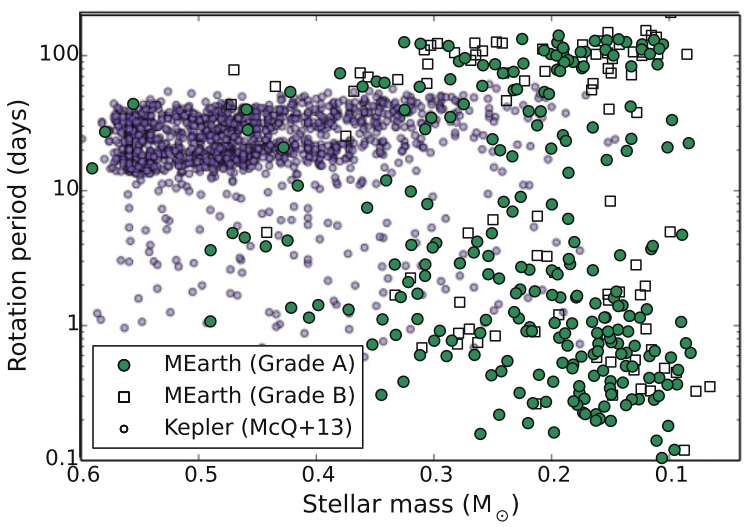
\includegraphics[width=.8\textwidth]{figures/mdwarfrotation.png}
  \caption[Empirical distribution of M dwarf photometric rotation periods.]
      {Rotation period versus stellar mass for solar neighbourhood and Kepler field
    M dwarfs. Periods of the Kepler stars are intentionally capped at \prot{} $=70$ days.
    The distribution of \prot{} appears to be bi-modal featuring a
    population of fast (\prot{} $\lesssim 3$ days) and slowly (\prot{} $\gtrsim 50$ days)
    rotating M dwarfs with a dearth of stars at intermediate \prot{.} These features are
    thought to be indicative of two distinctly aged populations. 
    \citep[Image credit:][]{newton16a}}
\label{fig:rotation}
\end{figure}

Another important point regarding active regions is that their lifetimes are often
one to a few stellar rotation timescales with those timescales being extended for later
type stars \citep{giles17}. That is that active regions on M dwarfs appear to be long-lived
compared to around Sun-like stars.
The evolution of active regions over rotation cycles implies that the associated
stellar activity can vary on similar timescales. %As seen in Fig.~\ref{fig:rotation},
M dwarf active region lifetimes can range from days to months and given that those
lifetimes are primarily determined by the active region sizes as they
diffuse into the photosphere \citep{berdyugina05}, larger volume/surface ratios results in
longer lifetimes \citep{petrovay97,giles17}. The lifetimes of M dwarf active regions will
have important implications when attempting to model stellar activity in RV time series in
subsequent chapters. \\

\emph{Gravitational redshift}:
the contraction and expansion of stars throughout their evolution will introduce an RV activity
signal. Even small variations at the level of hundredths of a percent will have manifestations
at the 10 cm s$^{-1}$ level which is sufficient to mask an Earth-like planet around a Sun-like star
\citep{lindegren03}. In low mass stars, the suppression of surface convection by strong magnetic fields
may result in stellar radius fluctuations and consequently an activity signal due to gravitational
redshift that varies on the timescale of variations in the star's magnetic field strength of days to
years \citep{cegla12}. \\


\emph{Magnetic Cycles}:
the Sun undergoes a long-term magnetic cycle with an 11 year period as measured by the
fractional coverage or number of sunspots and faculae visible on its surface \citep{hathaway10}.
At solar maximum, the 
peak in magnetic activity over the solar cycle, the Sun i) experiences strong prominences
and coronal mass ejections and ii) contains a large number of active regions that contribute
to a higher level of activity in RV time series as well as in other observables
\citep{maunder04}. Long-term magnetic activity cycles have been observed in long-baseline
spectroscopic monitoring programs \citep{santos10}. From solar observations, the flux in the
\caii{} H \& K lines are known to correlate with the number of sunspots. Numerous results from
similar surveys have 
demonstrated that the majority of Sun-like stars do exhibit magnetic activity cycles
with a range of periods from $\sim 7-30$ years \citep{duncan91,lockwood97,balinunas98}. \\

As it pertains to RV planet searches, activity cycles have been 
observed and characterized in Sun-like stars \citep{baliunas95}. 
Even when complete cycles remain unresolved, subsections of the cyclic trends have been seen in
certain mature RV surveys to be correlated with
the \Rhk{} spectroscopic activity indicator \citep[e.g.][]{lovis11}.
A common tactic to correct for such long-term activity trends in RV time series is to use a linear
relation between the RVs and the contemporaneous \Rhk{} time series although residual jitter
often persists \citep{dumusque12}. The corresponding RV signal from magnetic cycles can reach tens of
\mps{.} Luckily, when searching for
planets whose orbital timescales are much less than the period of the star's magnetic cycle, the
corresponding activity is not often a major concern. \\


\section{Point-form Thesis: Introduction}
\begin{itemize}
\renewcommand\labelitemi{--}
\item~\ref{sect:exoplanets} \textbf{Exoplanets}: exoplanets in the local universe are 
  extremely abundant and quite diverse compared to the planets in our own solar system.
\item~\ref{sect:Mdwarfs} \textbf{M dwarf stars}: M dwarfs represent superlative opportunities
  to characterize planetary systems in detail if we can mitigate their prominent stellar activity
  signatures.
\item~\ref{sect:detection} \textbf{Methods of Detecting Exoplanets}: there exists a 
number of methods of detecting exoplanets, each with its own sensitivities and biases.
\item~\ref{sect:rv} \textbf{Exoplanet Detection via Stellar Radial Velocity}: the 
  gravitational influence of planetary companions on their host star induces a periodically
  varying Doppler shift that may be detectable and used to measure an exoplanet's minimum mass
  and orbital properties.
\item~\ref{sect:spectrograph} \textbf{Measuring Radial Velocities}: hi-resolution 
  spectrographs are used to measure the Doppler shift of stellar absorption features.
  The precision of such measurements is often impeded by sources of error from the
  instrumentation, counting statistics, telluric contamination, and stellar activity.
\end{itemize}
  % 28-pages
%\input{chapters/GP}
%\chapter[Simulating the SPIRou Legacy Survey-Planet Search]{Predictions of planet detections with near infrared radial velocities in the up-coming$^*$\blfootnote{$^*$Now ongoing.} SPIRou legacy survey-planet search} \label{chap:BS}
%\author{Ryan Cloutier\altaffilmark{1,2,3}}
%\author{\'{E}tienne Artigau\altaffilmark{3}}
%\author{Xavier Delfosse\altaffilmark{4}}
%\author{Lison Malo\altaffilmark{3,5}}
%\author{Claire Moutou\altaffilmark{5,6}}
%\author{Ren\'{e} Doyon\altaffilmark{3}}
%\author{Jean-Francois Donati\altaffilmark{7,8}}
%\author{Andrew Cumming\altaffilmark{9}}
%\author{Xavier Dumusque\altaffilmark{10}}
%\author{\'Elodie H\'ebrard\altaffilmark{11}}
%\author{Kristen Menou\altaffilmark{2,1}}

\iffalse
\begin{abstract}
  The SPIRou near infrared spectro-polarimeter is
  destined to begin science operations at the Canada-France-Hawaii Telescope
  in mid-2018. One of the instrument's primary science goals is to discover the closest
  exoplanets to the Solar System by conducting a 3-5 year long radial velocity
  survey of nearby M dwarfs at an expected precision of $\sim 1$ \mps{;} the SPIRou
  Legacy Survey-Planet Search (SLS-PS). In this study we conduct a detailed Monte-Carlo
  simulation of the SLS-PS using our current understanding of the occurrence rate
  of M dwarf planetary systems and physical models of stellar activity.
  From simultaneous modelling of planetary signals and activity, we predict the population
  of planets detected in the SLS-PS. With our fiducial survey strategy and expected
  instrument performance over a nominal survey length of $\sim 3$ years,
  we expect SPIRou to detect $85.3^{+29.3}_{-12.4}$ planets including
  $20.0^{+16.8}_{-7.2}$ habitable zone planets and $8.1^{+7.6}_{-3.2}$ Earth-like planets
  %($m_p \in [1,5]$ M$_{\oplus}$)
  from a sample of 100 M1-M8.5 dwarfs out to 11 pc. By studying
  mid-to-late M dwarfs previously inaccessible to existing optical velocimeters, SPIRou will
  put meaningful constraints on the occurrence rate of planets around those stars
  including the value of $\eta_{\oplus}$ at an expected level of precision of $\lesssim 45$\%.
  We also predict a subset of $46.7^{+16.0}_{-6.0}$ planets may be accessible with
  dedicated high-contrast imagers on the next generation of ELTs including $4.9^{+4.7}_{-2.0}$ potentially imagable
  Earth-like planets. Lastly, we compare the results of our fiducial survey strategy to other foreseeable survey
  versions to quantify which strategy is optimized to reach the SLS-PS science goals.
  The results of our simulations are made available to the community on
  \href{https://github.com/r-cloutier/SLSPS\_Simulations}{github}. 
  %and/or the science goals
  %of other radial velocity planet searches with other up-coming instruments.
\end{abstract}
\fi

\blfootnote{The contents of this chapter are copied verbatim from the published paper \citep{cloutier18a}.}

\section{Introduction} 
The radial velocity method of detecting exoplanets is one of the most
successful methods of exoplanet detection
and has been widely used since the first discovery of an
exoplanet around a main-sequence star over two decades ago \citep{mayor95}. 
Since then numerous international teams have successfully built and used
precision velocimeters to grow the population of radial velocity (RV) planets
(e.g. HARPS; \citealt{mayor03}, HARPS-N; \citealt{cosentino12}, HIRES; \citealt{vogt94}).
Up until recently the majority of 
these precision velocimeters have operated in the visible wavelength
regime where their sensitivity is maximized for the discovery of planets
around Sun-like stars. \\

In recent years much interest has been generated regarding the population of
exoplanets around M dwarfs. M dwarfs, with effective temperatures
$\lesssim 3800$ K and masses $\lesssim 0.6$ M$_{\odot}$, outnumber Sun-like
stars in the Solar neighbourhood (within $\sim 10$ pc) nearly 4:1
\citep{henry09}. Furthermore, M dwarfs are known to frequently host multiple
small ($r_p \leq 4$ R$_{\oplus}$) planets \citep[e.g.][]{dressing15a, gaidos16}
including a large fraction of planets within the star's habitable zone (HZ)
which itself spans shorter orbital periods than around the more luminous
Sun-like stars \citep{kasting93, kopparapu13}.
Lastly the amplitude of the radial velocity signal induced by a given planet
is larger around M dwarfs than around Sun-like stars owing to their smaller
masses. These favorable qualities have many astronomers 
committed to uncovering the M dwarf exoplanet population with purpose-built
transit (e.g. MEarth; \citealt{irwin15}, ExTrA \citealt{bonfils15},
TRAPPIST; \citealt{gillon11}, SPECULOOS; \citealt{gillon13a})
and radial velocity instrumentation (e.g.
SPIRou; \citealt{delfosse13, artigau14}, NIRPS; \citealt{bouchy17}, CARMENES;
\citealt{quirrenbach14}, HPF; \citealt{mahadevan12}, IRD; \citealt{tamura12}). \\

One particular precision velocimeter optimized for the detection of
exoplanets around M dwarfs in radial velocity is \emph{SPIRou} \citep[Un
  Spectro-Polarim\`{e}tre Infra-Rouge;][]{delfosse13, artigau14}. SPIRou
is a high-resolution near-infrared velocimeter whose first-light is scheduled on
the Canada-France-Hawaii Telescope (CFHT) in 2018. A significant fraction of SPIRou's
allocated time will be spent surveying
nearby M dwarfs searching for new exoplanets in a campaign known as the
\emph{SPIRou Legacy Survey-Planet Search} (SLS-PS). With the increased
sensitivity to cool M dwarfs enabled by nIR detectors, the planet detections
resulting from the
SLS-PS will be able to constrain the occurrence rate of planets around stars
later than $\sim$ M4.5 and find the closest exoplanetary
systems, beyond Proxima Centauri \citep[1.3 pc;][]{angladaescude16}, which
may be amenable to direct imaging with the next generation of imagers on-board
an Extremely Large Telescope (ELT). \\

In this study we present a comprehensive simulation of the SLS-PS to estimate its
planet yield as well as the bulk properties of the detected SPIRou planet population.
These simulations were performed for a variety
of survey strategies which enabled the SPIRou science team to establish an
experimental setup which optimizes both the detection sensitivity and survey
yield given the nominal time allocation of the SLS-PS. The main results of this
study are based on the survey version deemed to be optimal for meeting the 
science goals of SPIRou. However, the results of the
various surveys are summarized in the final Sect.~\ref{BSsect:surveys}. Comparison
of the various survey versions may be useful to inform other up-coming radial velocity
planet searches similar to the SLS-PS. \\

The paper is organized as follows:

\begin{itemize}
\item Sect.~\ref{BSsect:spirou} gives an overview of the important aspects of the
  SPIRou spectro-polarimeter.
\item Sect.~\ref{BSsect:starsample} describes the stellar input catalog.
\item Sect.~\ref{BSsect:survey} describes the simulated SLS-PS.
\item Sect.~\ref{BSsect:planetsample} describes the population of simulated
  planetary systems. 
\item Sects.~\ref{BSsect:GP}-\ref{BSsect:detection} describe how we mitigate the
  effects of stellar activity and detect planets.
\item Sects.~\ref{BSsect:sensitivity}-\ref{BSsect:yield} describe the results of
  the survey.
\item Sect.~\ref{BSsect:2occ} considers the effect of an increased planet frequency
  on the survey results.
\item Sect.~\ref{BSsect:measurements} describes how well we can measure
  planet occurrence rates based on the results of the SLS-PS.
\item Sect.~\ref{BSsect:imaging} discusses the potential for targeting SPIRou
  planets in direct imaging campaigns with ELTs
\item and Sect.~\ref{BSsect:surveys} compares the merits of various potential
  versions of SLS-PS with the fiducial version presented throughout this paper.
\end{itemize}

\section{Un Spectro-Polarim\`{e}tre Infra-Rouge} \label{BSsect:spirou}
SPIRou is an up-coming nIR \'echelle spectro-polarimeter and high-precision velocimeter whose first
light is scheduled for 2018 on the Canada-France-Hawaii Telescope on Maunakea.
The instrument is optimized to observe exoplanets via the radial
velocity technique around low mass stars and to study the magnetic fields of young embedded protostars
\citep{delfosse13}. 
The design of SPIRou is intended to address its main science goals of detecting and characterizing
M dwarf exoplanetary systems and to investigate the role that magnetic fields have on the processes of
star and planet formation. SPIRou can be considered a heritage instrument which is built upon the success
of the previous generation of optical spectro-polarimeters and high-precision velocimeters such as the ESPaDOnS
spectro-polarimeter \citep{donati06} as well as the RV spectrographs SOPHIE \citep{bouchy06}
and HARPS \citep{mayor03}. \\

Here we provide a brief overview of the main instrument specifications as they pertain to the detection of
new exoplanetary systems around nearby M dwarfs.  Details of the optical and mechanical design
of the instrument can be found in \cite{artigau14}. 
The instrument itself is a fiber-fed, bench-mounted, double-pass, cross-dispersed, spectro-polarimeter
that is cryogenically cooled to an operation temperature of 80 K and provides simultaneous spectroscopic and
polarimetric observations. The optical fiber-link connecting the
Cassegrain unit---used for polarimetric analysis and guiding---to the calibration module and spectrograph is made
from purified fluoride; a special optical material featuring improved transmission at wavelengths $>2.0$ $\mu$m thus
enabling the inclusion of the $K$ band. The inclusion of the $K$ band in the SPIRou spectral coverage
is unique among most nIR velocimeters and is highly desirable for the velocimetry of late M dwarfs as
a large fraction of the RV information content is contained in the $K$ band \citep{artigau18}.
With the broad continuous spectral coverage of SPIRou spanning the nIR $YJHK$ bands
($0.98-2.35 \mu$m), SPIRou will pioneer infrared planet searches by targeting low mass stars whose flux
peaks in the nIR wavelength domain. In order to detect Earth-size planets, SPIRou is required to achieve a
long-term RV precision of 1 \mps{} while simultaneously monitoring the star's intrinsic activity which is enabled
by its high spectral resolution ($\lambda/ \Delta \lambda = 70,000$). \\

Thanks to its spectro-polarimetric capabilities, SPIRou is also optimized for characterizing stellar activity---an
obvious asset for studying M dwarfs---and particularly late-type M dwarfs which are known for their significant levels
of magnetic activity \citep{west15}. This will allow users to i) minimize the impact of activity on RV curves and
ease planet detections and ii) to characterize the impact of stellar activity on the close-in habitable zone
planets that SPIRou will detect.


\section{Stellar Input Catalog} \label{BSsect:starsample}
\subsection{Stellar Sample} \label{BSsect:starsamplesub}
The SPIRou input catalog used in our simulated SLS-PS (see Sect.~\ref{BSsect:survey})
contains 100 stars visible from CFHT on Maunakea
($\delta \gtrsim -30^{\circ}$). We note that the stellar sample used in these simulations is intended to be an
approximation to the true SPIRou input catalog which has yet to be formalized exactly. The stars chosen
were selected based on their high scores in the
SPIRou merit function. The merit function is based on being able to detect the RV semi-amplitude
from the gravitational pull of an 3 M$_{\oplus}$ planet at an equilibrium temperature of 250 K (Malo et al. in prep).
Of the optimum selection of 120 stars, approximately 20 were
deemed to result in poor detection sensitivities based on 
the measured fractions of simulated planets detected around those stars in preliminary simulations
of the SLS-PS. The primary
culprit for the rejection of these stars was their large projected rotation
velocities \vsini{,} which have a large detrimental effect on the RV measurement
precision and hence on our ability to detect planets.  \\

Properties of stars in the SPIRou input catalog are presented in Fig.~\ref{BSfig:stellardist}.
For comparison purposes, in Fig.~\ref{BSfig:stellardist} we include six nearby M dwarf
planetary systems with at least one known planet in or near the HZ: 
Proxima Centauri \citep{angladaescude16}, Ross 128 \citep{bonfils17a},
GJ 273 \citep{astudillodefru17a}, LHS 1140 \citep{dittmann17a}, TRAPPIST-1 \citep{gillon17},
and K2-18 \citep{montet15, cloutier17b}.
The global properties of the 100 stars were defined from the \cite{boyajian12} relation (effective
temperature and radii, when [Fe/H] is fixed to the solar value) and the \cite{delfosse00} relation
(estimated stellar mass based on absolute $J$ magnitude).
Projected rotational velocities and rotation periods were taken
from an exhaustive literature search or derived from the CFHT-CoolSnap program
\citep{moutou17}. In our sample
we consider stars with masses between 0.08-0.57 M$_{\odot}$ with $J$ band magnitudes $4.2-10.3$ in
a range of distances spanning $\sim 1.8-11$ pc. \\

\begin{figure*}
  \centering
  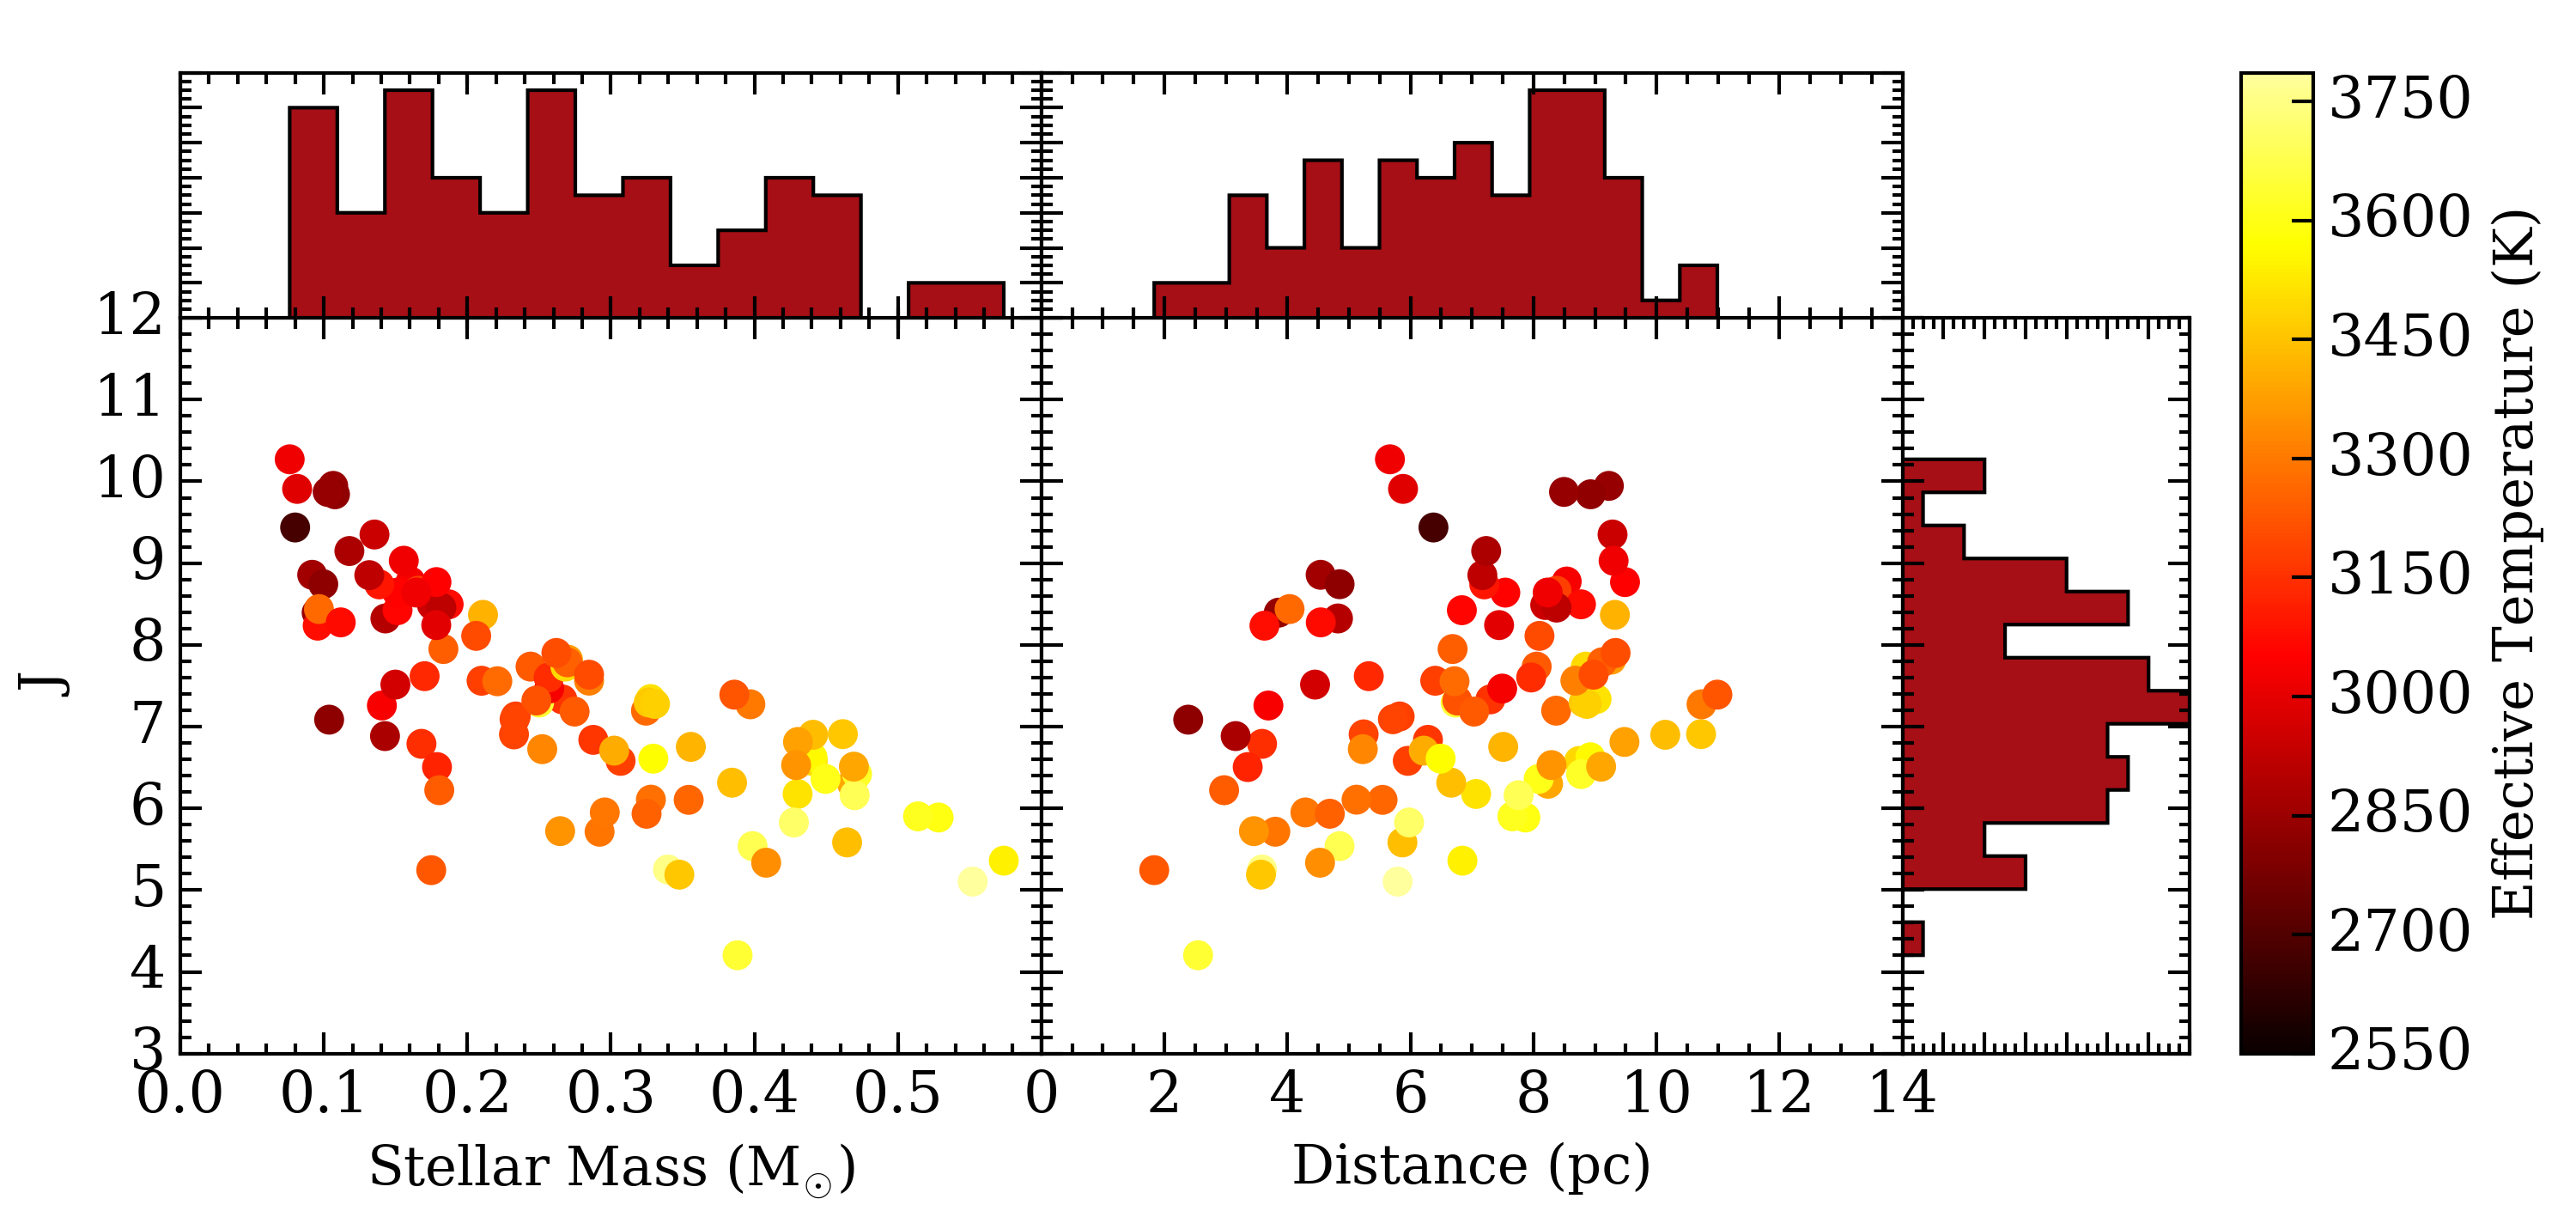
\includegraphics[width=0.8\hsize]{figures/stellarpop_bkgd.png}%
  \hspace{-0.8\hsize}%
  \begin{ocg}{fig:staroff}{fig:staroff}{0}%
  \end{ocg}%
  \begin{ocg}{fig:staron}{fig:staron}{1}%
    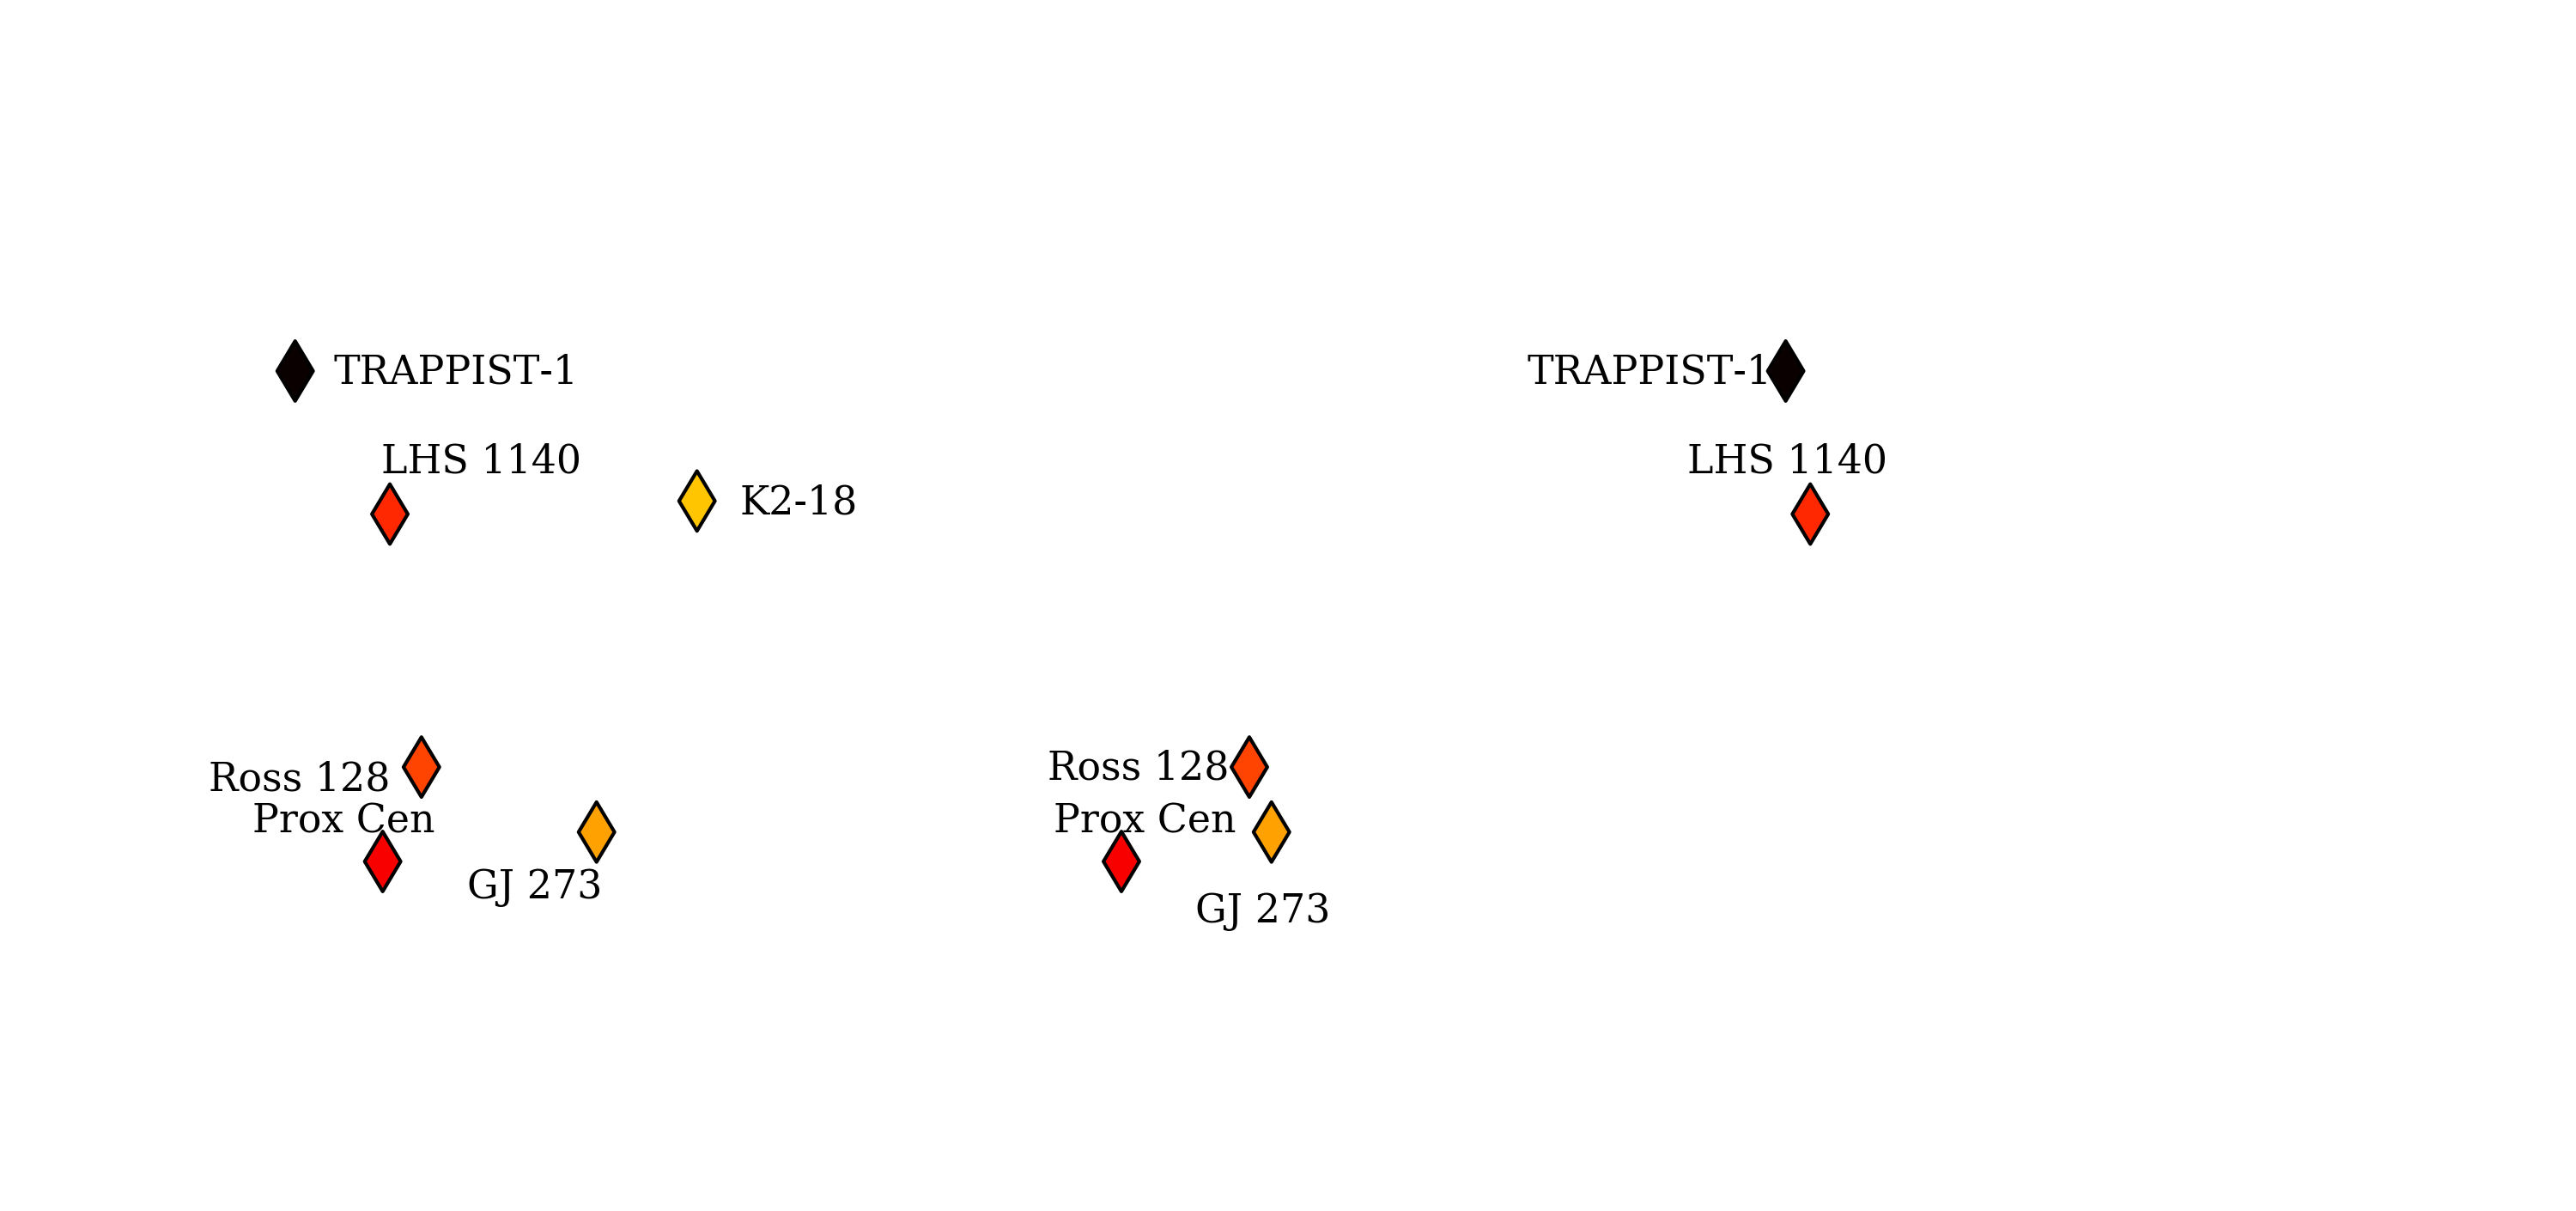
\includegraphics[width=0.8\hsize]{figures/stellarpop_stars.png}%
  \end{ocg}
  \hspace{-0.8\hsize}%
  \caption[Stellar parameters of sources targetted in the simulated \emph{SPIRou Legacy Survey-Planet Search}.]
      {\small Scatter plots and histograms depicting the distribution of SPIRou input catalog
    $J$ band magnitudes, stellar masses, distances, and effective temperatures for our fiducial 
    version of the \emph{SPIRou Legacy Survey-Planet Search}. Histograms are
    in linear units. Nearby M dwarf planetary systems with at least one known HZ planet
    are depicted with
    \ToggleLayer{fig:staron,fig:staroff}{\protect\cdbox{\emph{diamonds}}}. K2-18 at 34 pc does not
    appear in the scatter plot in right panel.}
  \label{BSfig:stellardist}
\end{figure*}

Rotational information for stars in our sample is an important characteristic for RV modelling
as stellar rotation strongly affects the activity arising from rotationally modulated active
regions observed in radial velocity \citep{saar97, meunier10, aigrain12, dumusque14}.
Rotation timescales also restrict the periodicities at which we can detect planets
due to difficulties in detecting RV planets with 
orbital periods close to the stellar rotation period or its harmonics \citep{vanderburg16}. 
However, the rotational information for our stellar sample is incomplete.
For stars with no known available rotation measurements (8/100 stars),
or with a \vsini{} upper limit only (2/100 stars),
we sample \prot{} from a \emph{modified} empirical distribution of M dwarf
rotation periods from ground-based photometry as a function of stellar mass
\citep{newton16a}. The nature of this `modification' is discussed in the subsequent
paragraph. The corresponding \vsini{} is then computed
from the sampled value of \prot{,} the known stellar radius, and the
inclination of the stellar spin--axis to the line-of-sight $i_s$ which we
draw from a geometrical distribution (i.e. uniform in $\cos{i_s}$).
For stars which only have a measured upper limit on \vsini{,} 
the \emph{modified} empirical distribution from which \prot{} is sampled is
truncated at the minimum \prot{} corresponding to the upper limit on \vsini{.} \\

The necessary modification to the empirical \prot{} distribution arises from
an observational bias in the \cite{newton16a} sample which favors rapidly rotating stars.
The detection of short photometric rotation periods (i.e. rapid rotators) is attained more
easily than long rotation periods because full phase coverage is more readily obtained over many
rotation cycles. Furthermore, in the case of early M dwarfs ($M_s > 0.25$ M$_{\odot}$), 
there is evidence for a positive correlation between the star's rotation rate and the
amplitude of its photometric variability \citep{newton16a}. Rapid rotators therefore
tend to exhibit larger amplitudes of variability thus making the signal more easily detectable.
The raw empirical distribution therefore does not represent the true underlying distribution of M
dwarf rotation periods in the Solar neighborhood. We attempt to account for this bias in a simplified
way by modifying the empirical \prot{} distribution by insisting that only
$\sim 25$\% of sampled rotation periods can be $<10$ days, as estimated from the volume-limited sample
of field M dwarfs with measured rotation velocities from \cite{delfosse98}. This constraint
reduces the fraction of fast rotators with \prot{} $< 10$ days by a factor of $\sim 2$. \\

The modification to the empirical \prot{} distribution is visualized in Fig.~\ref{BSfig:protcdf}.
Here we compare the empirical \prot{} distribution, based on the full stellar sample with detected
\prot{} from \cite{newton16a}, with the modified distributions of stars in the SPIRou input catalog
with either a \vsini{}
upper limit only or no available rotation data. The latter two distributions are nearly equivalent as
the majority of \vsini{} upper limits do not provide substantial new information regarding the star's \prot{}
and in both cases we insist that only $\sim 25$\% of sampled \prot{} can be $< 10$ days. We impose this
condition by noting that $\sim 60$\% of stars in the empirical distribution have \prot{} $<10$ days
and resample a particular fraction of those stars from the subset of the empirical distribution restricted
to \prot{} $\geq 10$ days. The fraction of stars with \prot{} $<10$ days that get resampled is
$1-0.25/0.6 \approx 0.58$. 

\begin{figure}
  \centering
  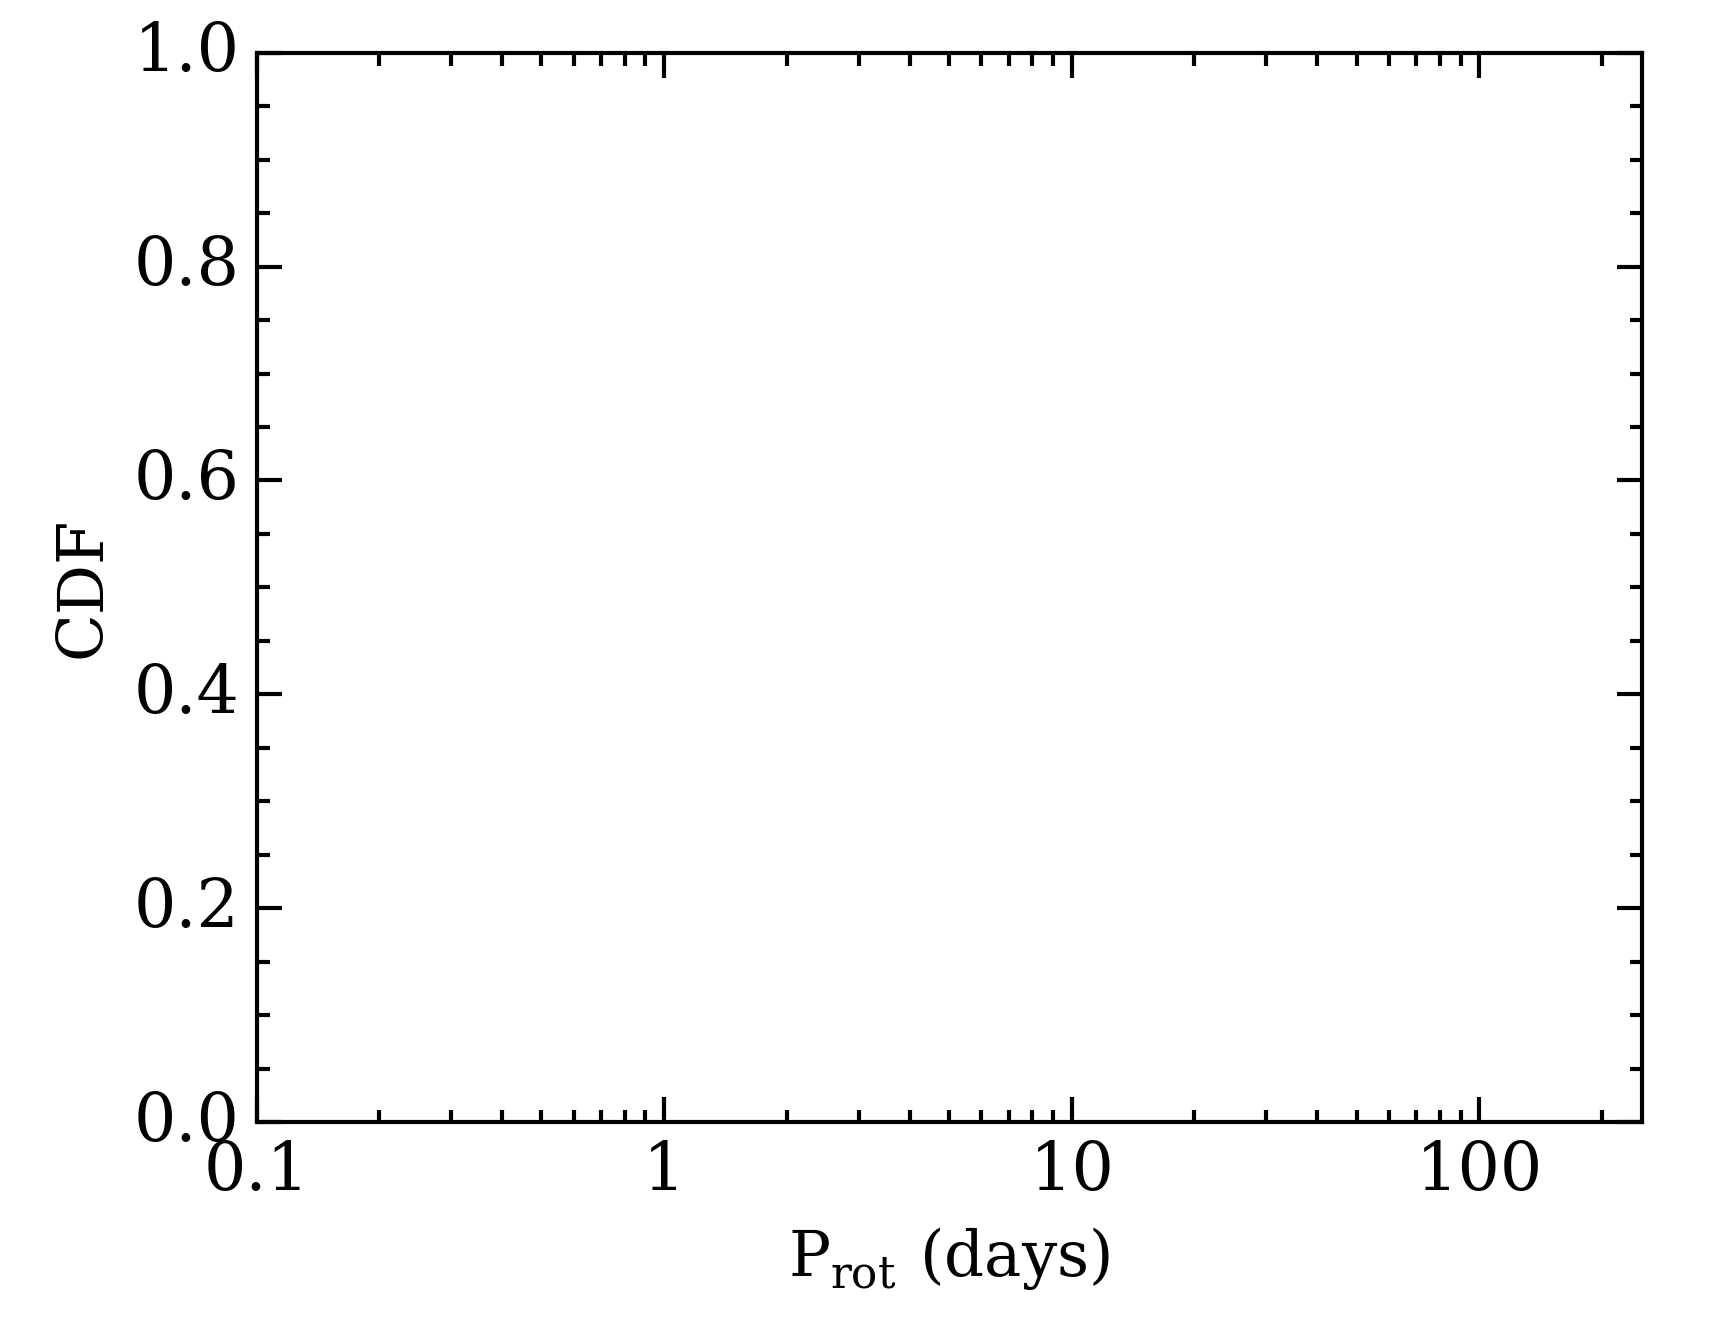
\includegraphics[width=0.8\hsize]{figures/ProtCDF_bkgd.png}%
  \hspace{-0.8\hsize}%
  \begin{ocg}{fig:1off}{fig:1off}{0}%
  \end{ocg}%
  \begin{ocg}{fig:1on}{fig:1on}{1}%
    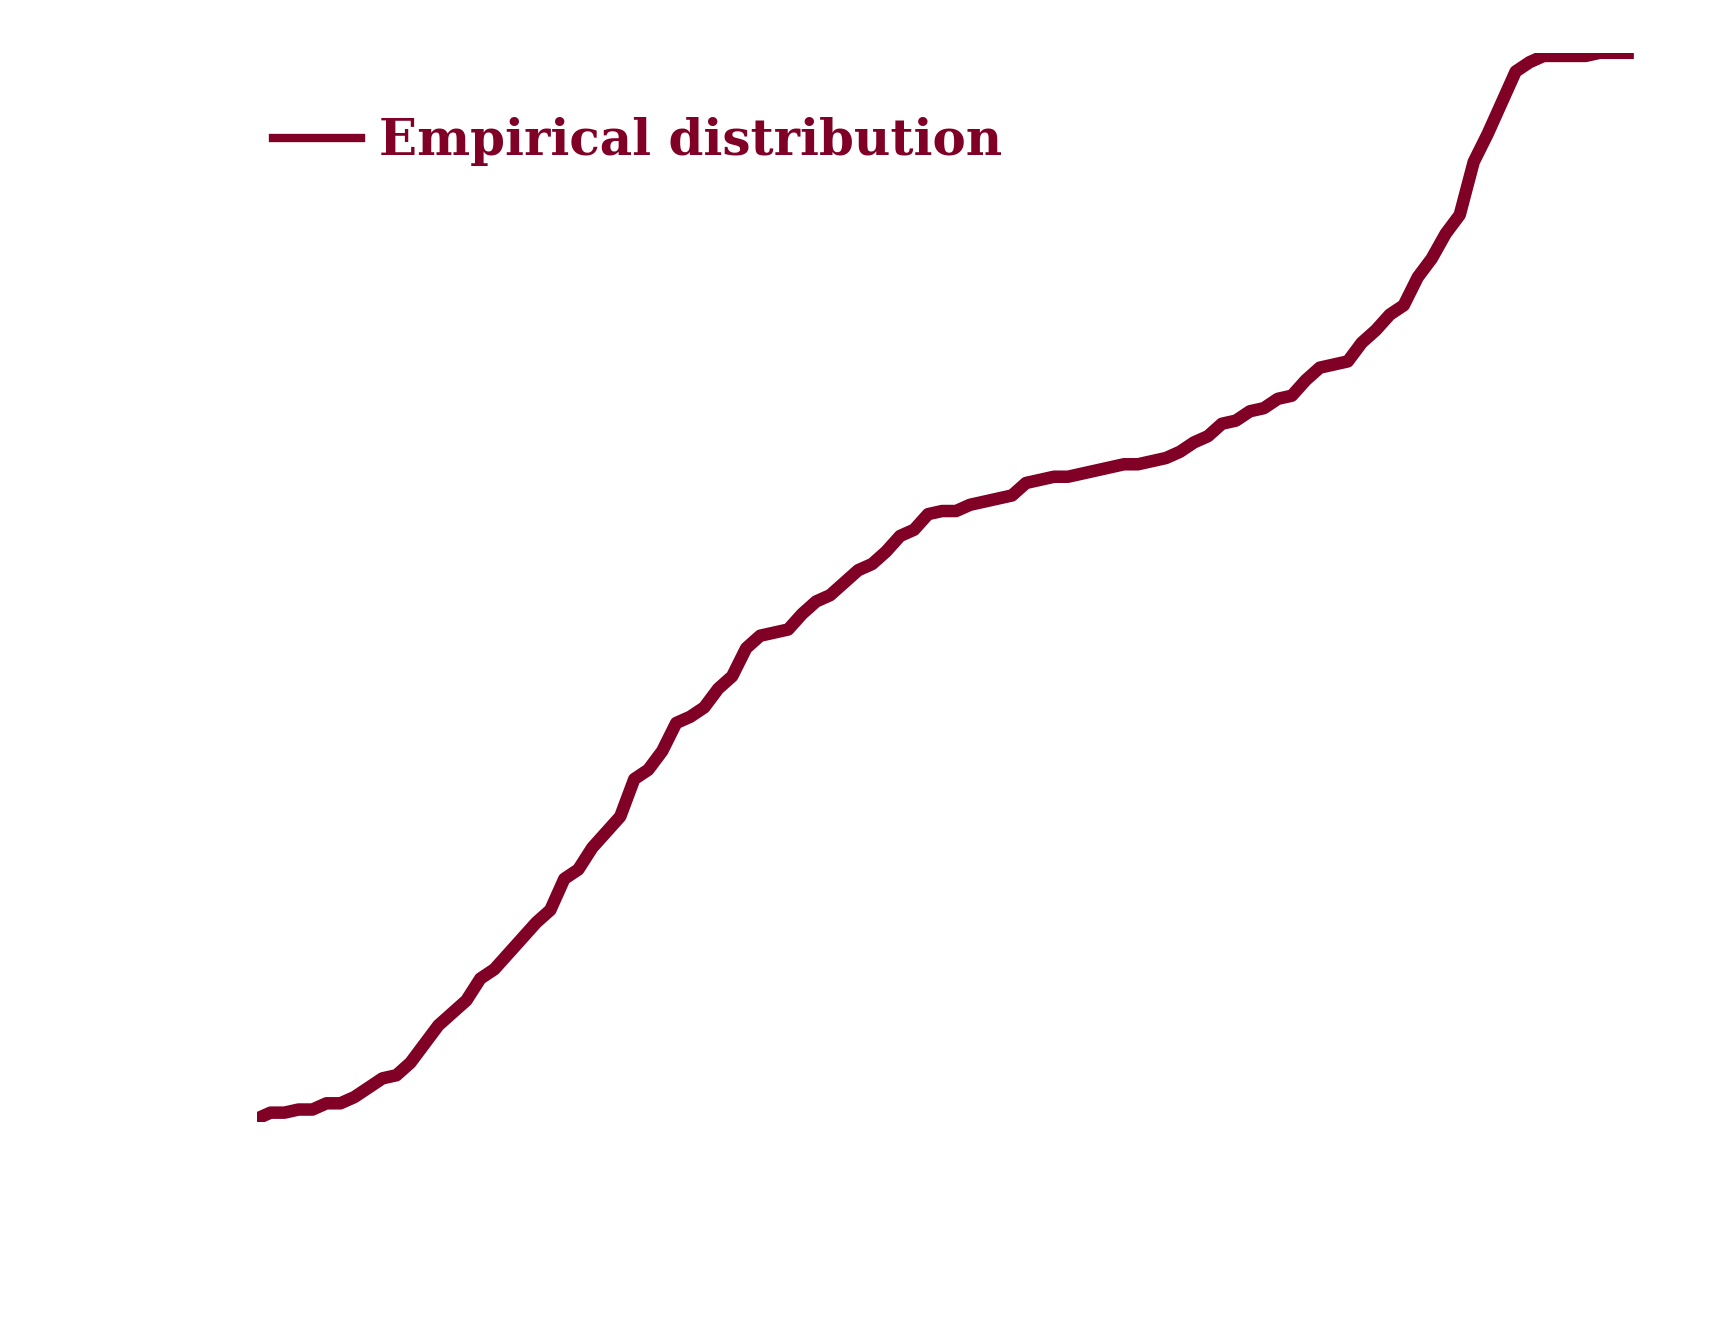
\includegraphics[width=0.8\hsize]{figures/ProtCDF_1.png}%
  \end{ocg}
  \hspace{-0.8\hsize}%
  \begin{ocg}{fig:2off}{fig:2off}{0}%
  \end{ocg}%
  \begin{ocg}{fig:2on}{fig:2on}{1}%
    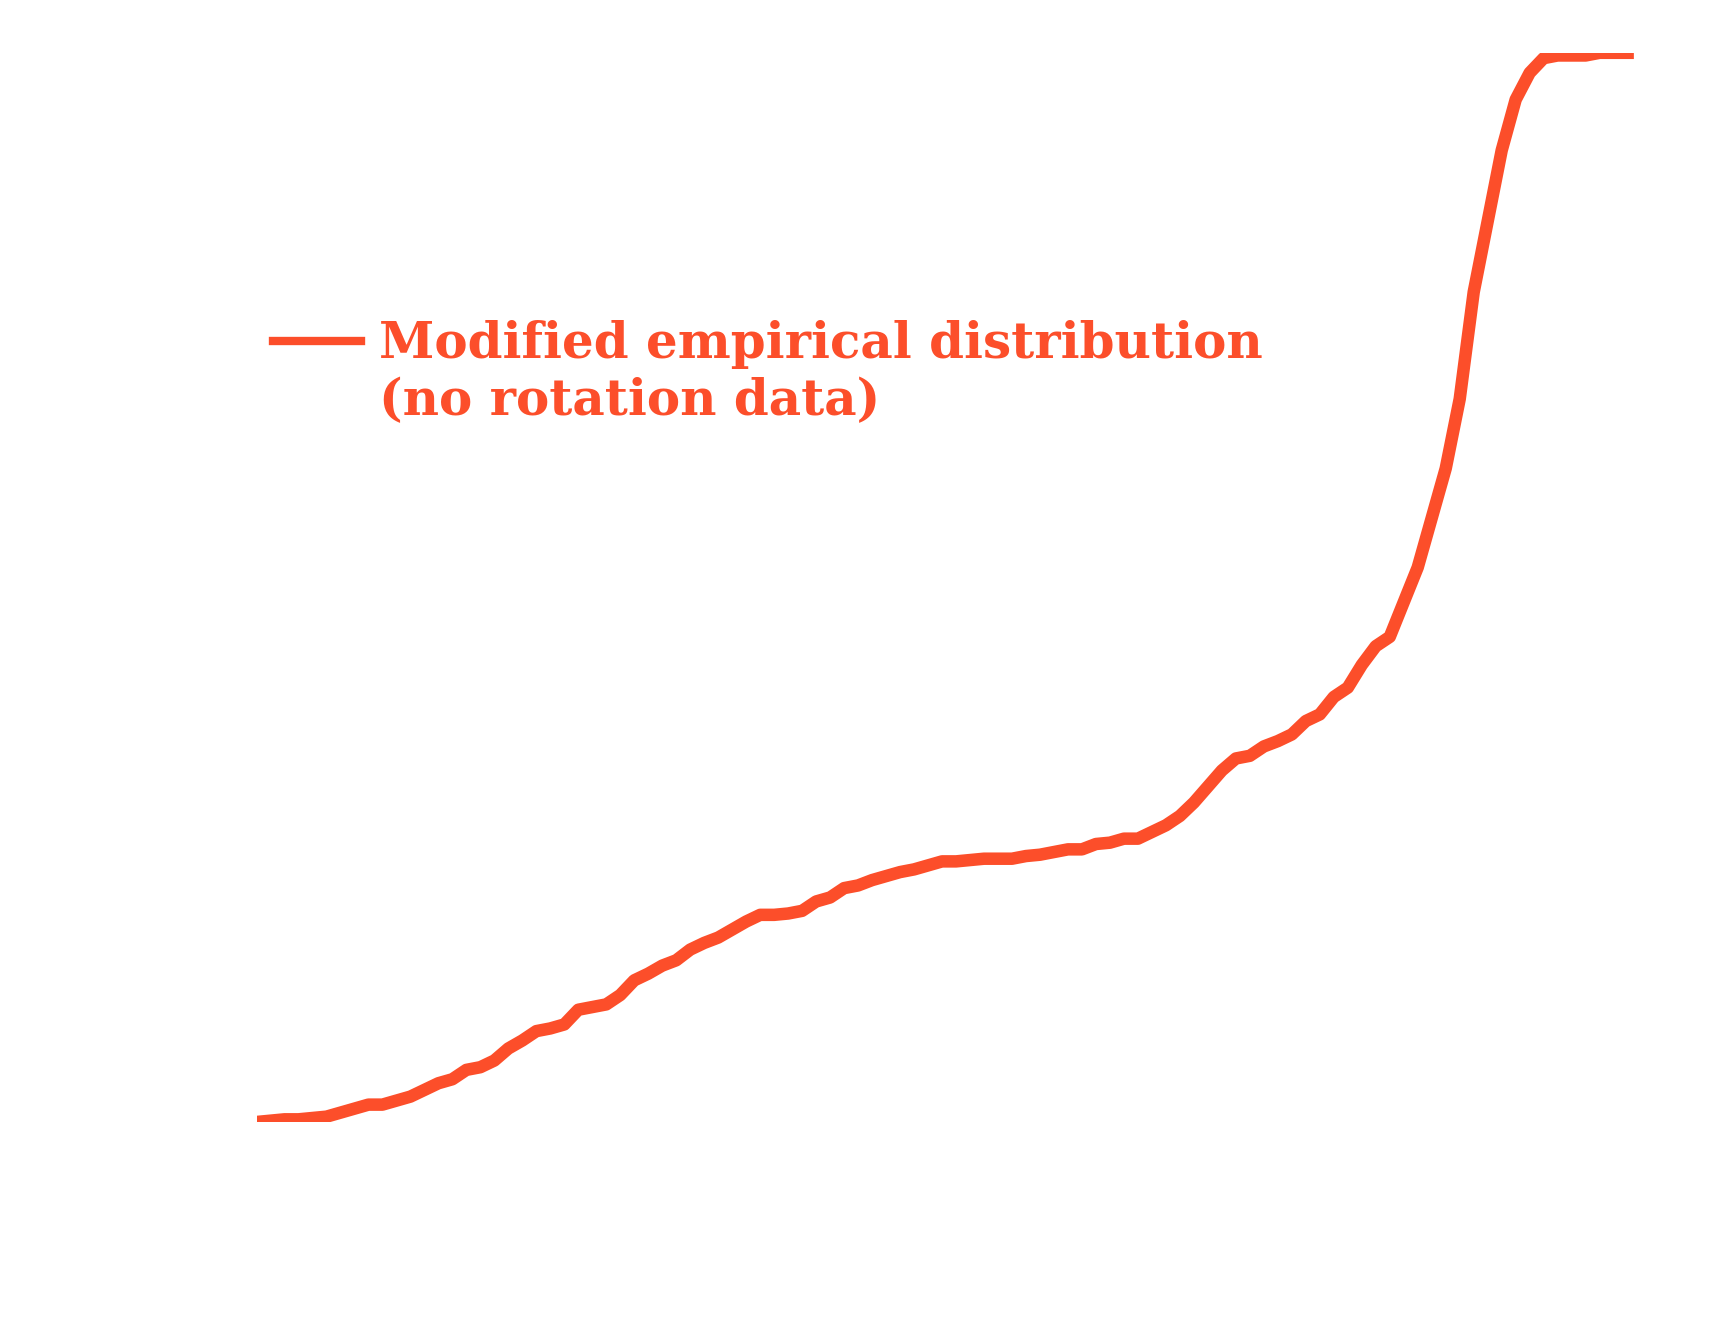
\includegraphics[width=0.8\hsize]{figures/ProtCDF_2.png}%
  \end{ocg}
  \hspace{-0.8\hsize}%
  \begin{ocg}{fig:3off}{fig:3off}{0}%
  \end{ocg}%
  \begin{ocg}{fig:3on}{fig:3on}{1}%
    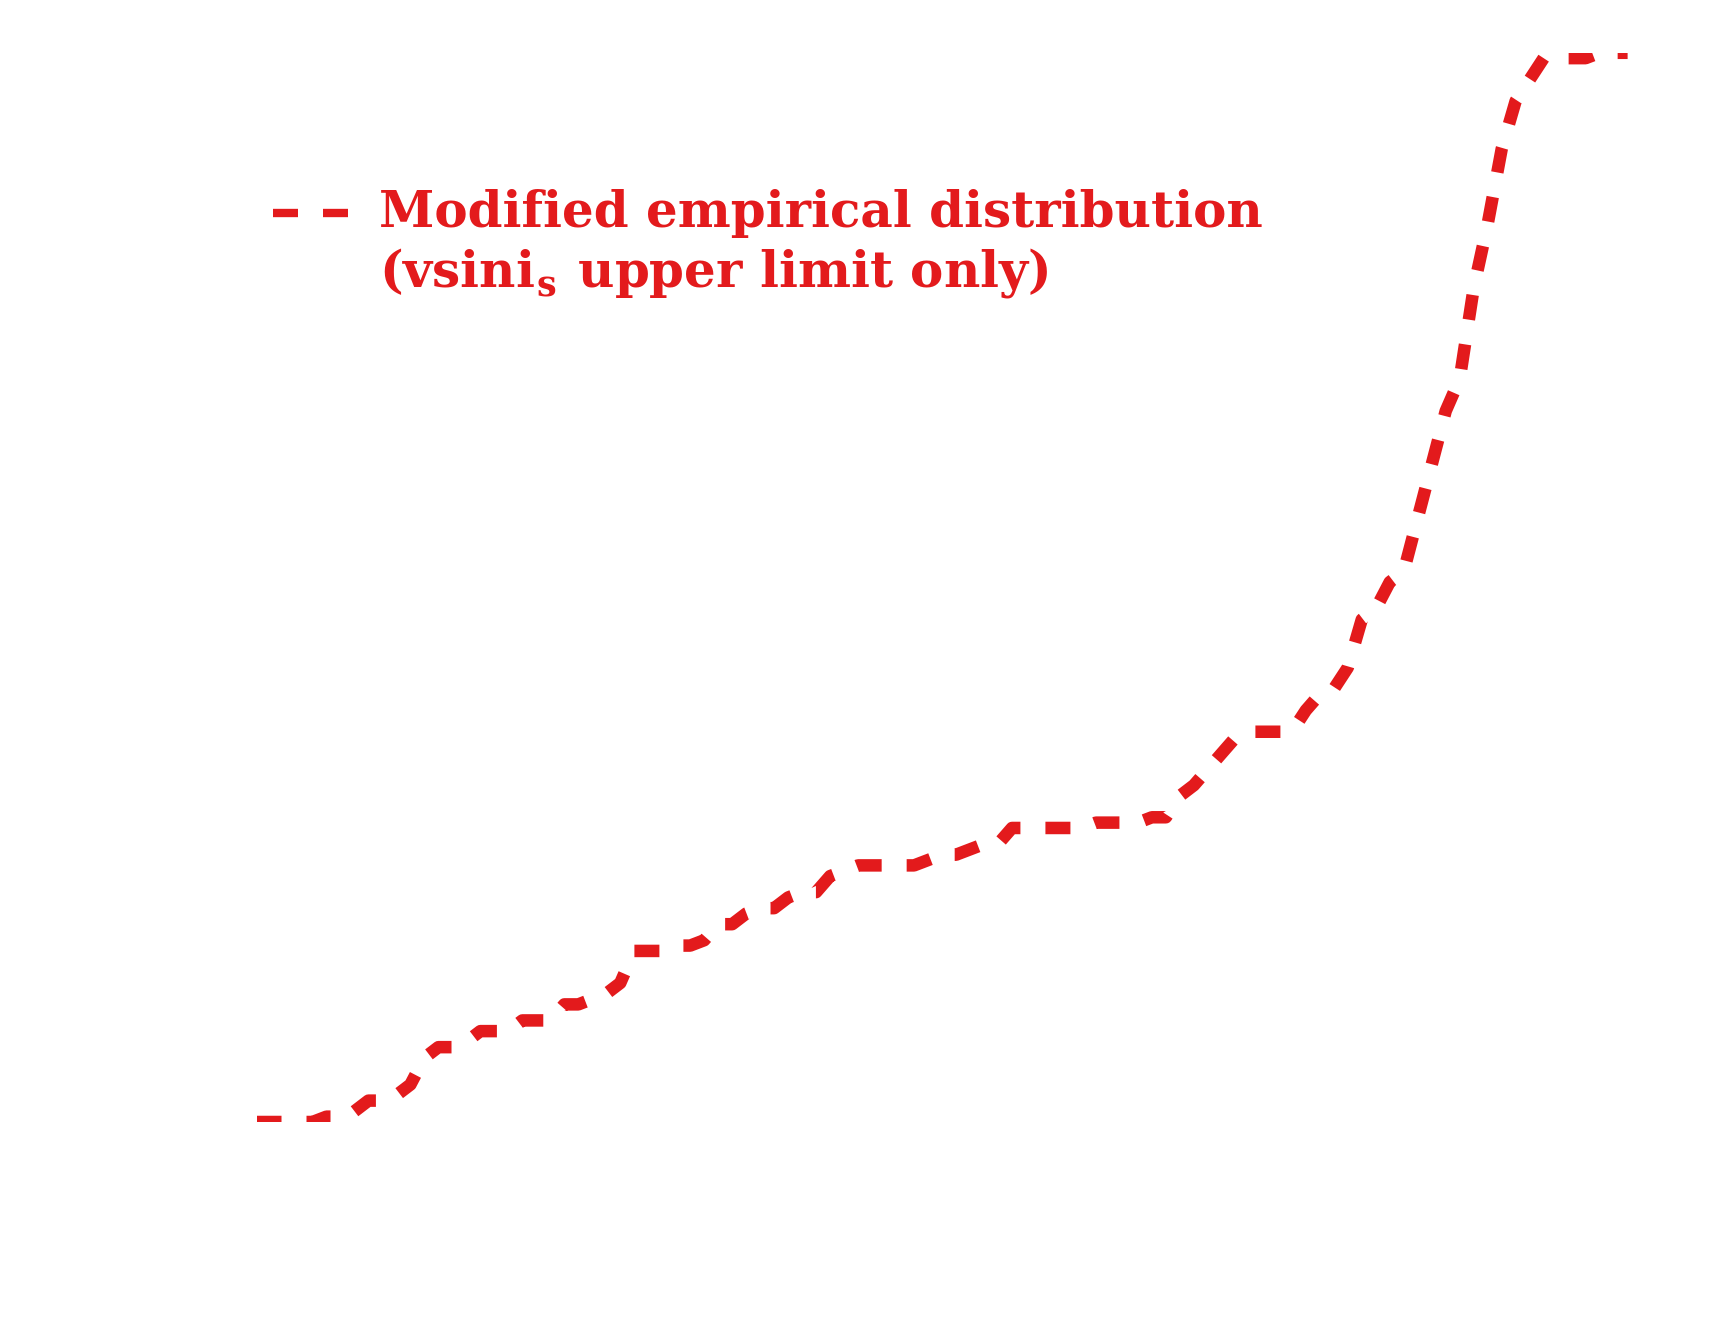
\includegraphics[width=0.8\hsize]{figures/ProtCDF_3.png}%
  \end{ocg}
  \hspace{-0.8\hsize}%
  \begin{ocg}{fig:4off}{fig:4off}{0}%
  \end{ocg}%
  \begin{ocg}{fig:4on}{fig:4on}{1}%
    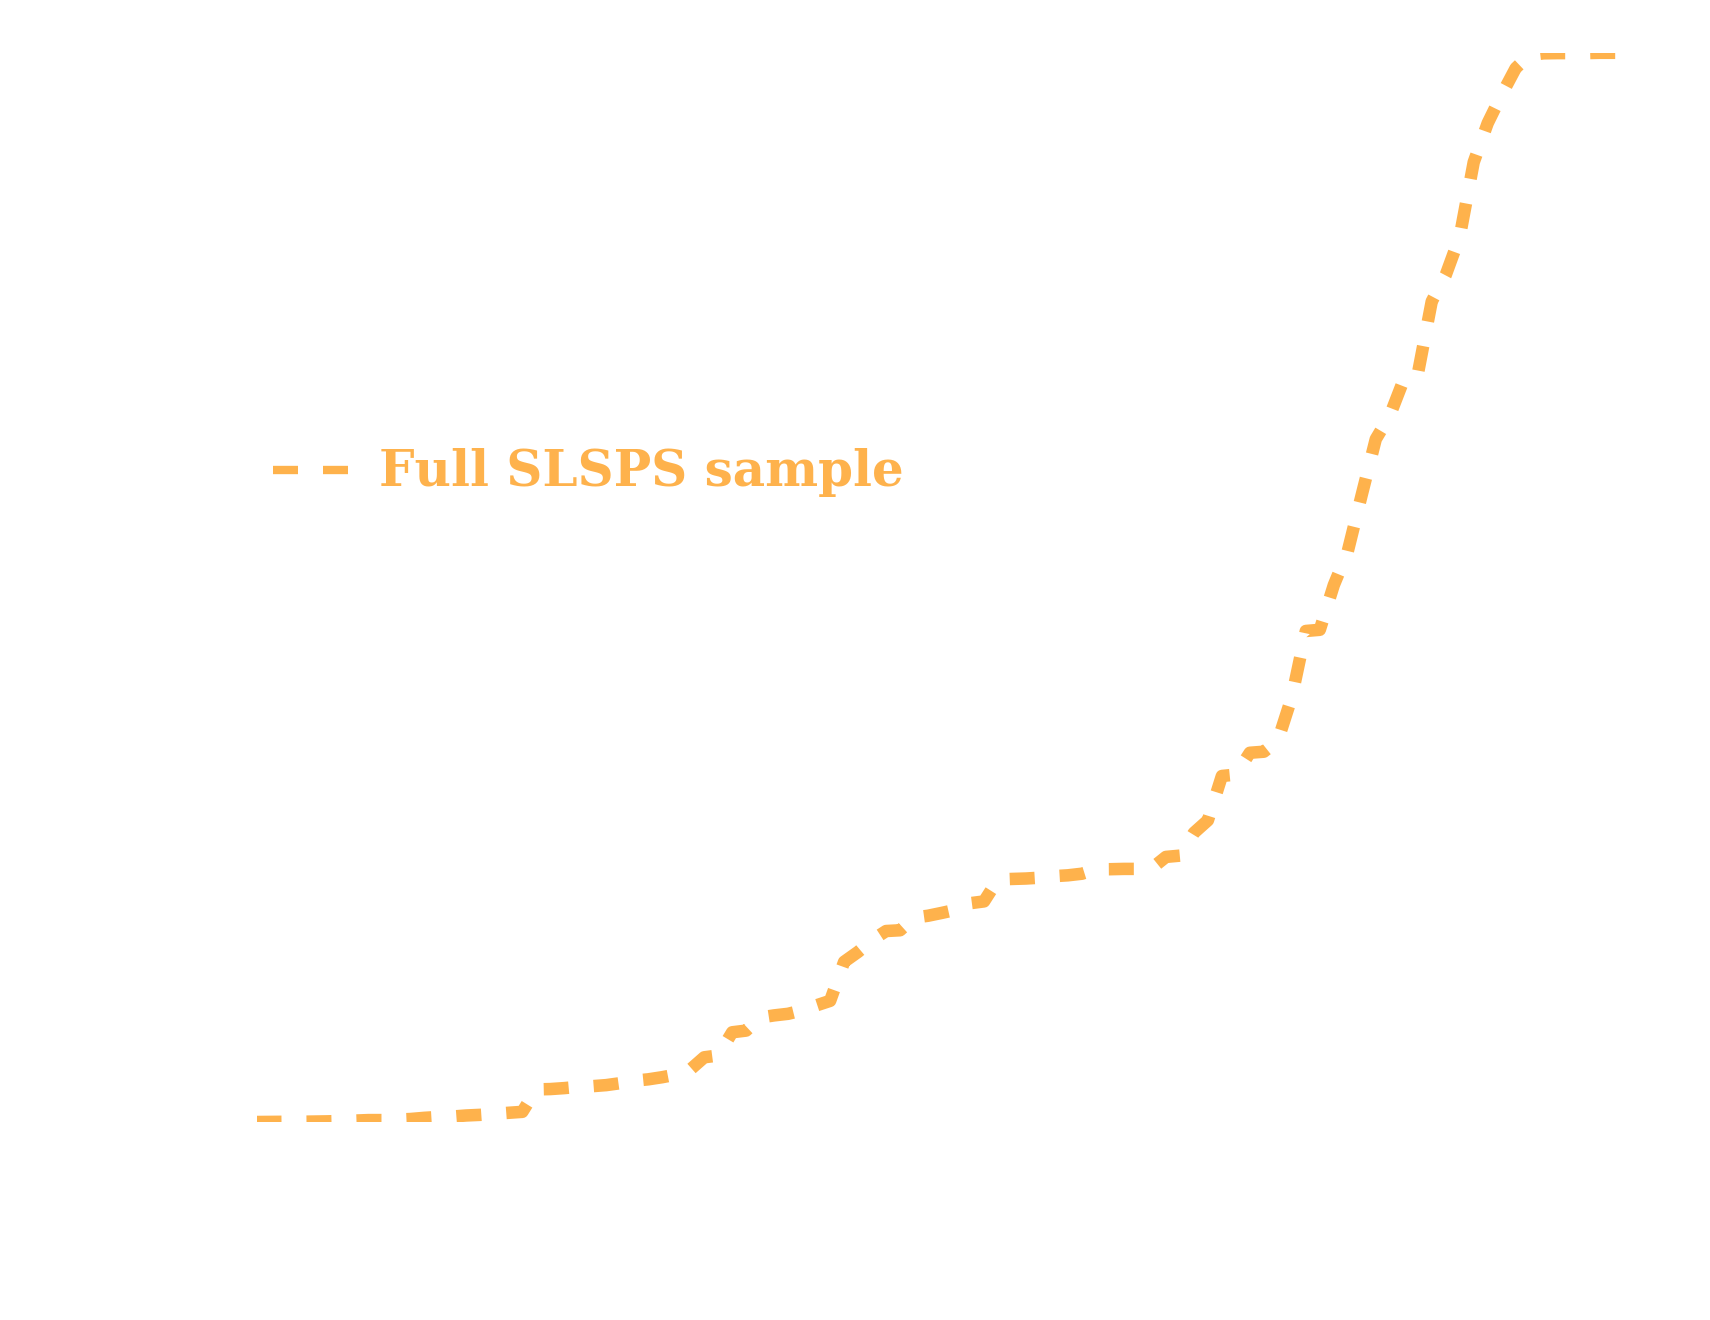
\includegraphics[width=0.8\hsize]{figures/ProtCDF_4.png}%
  \end{ocg}
  \hspace{-0.8\hsize}%
  \caption[M dwarf rotation period distributions.]
      {\small Cumulative distribution functions of the 
    \ToggleLayer{fig:1on,fig:1off}{\protect\cdbox{empirical distribution}} of M dwarf rotation periods
    from \cite{newton16a}, the modified empirical distribution of SPIRou stars with a 
    \ToggleLayer{fig:3on,fig:3off}{\protect\cdbox{\vsini{} upper limit}} measured, the
    modified empirical distribution of SPIRou stars with
    \ToggleLayer{fig:2on,fig:2off}{\protect\cdbox{no rotation data}} available, and the
    \ToggleLayer{fig:4on,fig:4off}{\protect\cdbox{full SLS-PS sample}}.}
  \label{BSfig:protcdf}
\end{figure}

\subsection{Physical Models of Stellar RV Activity} \label{BSsect:activity}
\subsubsection{\texttt{SOAP 2.0}: activity simulations} \label{BSsect:soap}
Active regions (ARs) in the stellar photosphere (e.g. star spots and faculae) and in
the hot chromosphere (e.g. plages) are expected to be present in M dwarfs. These surface inhomogeneities
have characteristic temperatures that differ from the star's effective temperature and therefore 
disrupt the symmetry of the visible stellar disk as they rotate in and out of view at the stellar rotation
period. One resulting source of RV activity from ARs, known as the \emph{flux effect} \citep{dumusque14},
results in an anomalous RV signal as the ARs block a fraction of Doppler-shifted
photons from the rotating stellar limbs. The strong local magnetic fields associated with ARs
at the stellar photospheric boundary also act to inhibit the upward flow of hot convective material
in an effect known as the suppression of \emph{convective blueshift} \citep{dravins81}. \\

In the limit of simple distributions of ARs, the observed RV structure from the two aforementioned effects 
is dependent on the fractional coverage of the visible stellar disk by the ARs and its first time
derivative \citep{aigrain12}. For each simulated RV time-series, we sample the relevant physical
parameters of the ARs (i.e. AR sizes and spatial distribution) and 
simulate the corresponding RV activity, full width at half maximum (FWHM), bi-sector inverse slope (BIS),
and photometric time-series arising from both the flux effect and from the suppression of convective blueshift 
using the \texttt{SOAP 2.0} code \citep{dumusque14}. The FWHM and BIS time-series are shape parameters of
the cross-correlation function between the observed stellar spectra and the template spectrum used to measure
the stellar RVs in an observing campaign. These ancillary time-series are sensitive to the presence of ARs but not to planets
making them useful diagnostics for distinguishing activity-induced RV signals from planetary signals.
In particular, the FWHM time-series will be used in
Sect.~\ref{BSsect:GP} to train our RV activity model and disentangle RV activity signals from planetary signals. \\

The \texttt{SOAP 2.0} code outputs time-series that are phase-folded to the input 
stellar rotation period. These time-series are initially treated as strictly periodic
and interpolated to the epochs of observation. In
this way we ignore any contribution from differential rotation whose amplitude has been shown to
decrease with decreasing stellar mass \citep{donati08, morin08, kitchatinov11}
before evoking rigid-body rotation in fully convective M dwarfs
($M_s \lesssim 0.2$ M$_{\odot}$). In Sect.~\ref{BSsect:lifetimes},
the strictly periodic condition is relaxed to account for the finite lifetimes of ARs and the existence of
long-term magnetic activity cycles. \\

Unfortunately, very little is presently known about the physical nature of ARs on M dwarfs but we do observe
quasi-periodic photometric variability which arises from evolving ARs \citep{oneal05}. We use the
empirical distribution of photometric amplitudes as a function of stellar mass from \cite{newton16a} to sample
the \emph{average} photometric variability amplitudes\footnote{For photometric variations measured in the near-IR
  with MEarth over a custom passband spanning $\sim 0.7-1 \mu$m known as the $i+z$ band \citep{nutzman08}.}
$A$ for each star in the simulated SLS-PS. The sampled value of $A$ is interpreted as an
average value because the phase in the star's magnetic activity cycle at the time of the \cite{newton16a}
observations is unknown. We then use $A$ to constrain the size of up to four ARs with each AR being treated as either
a cool spot or bright plage. The spatial distribution of
ARs is determined from random draws in latitude and longitude as  
Doppler imaging provides evidence for more uniformly distributed ARs on M dwarfs than on
Sun-like (FGK) stars \citep{barnes01, barnes04}, whose ARs tend to be more localized along the
stellar equator. We note however that such Doppler imaging observations are limited to rapid rotators
which are largely avoided in the selection of the SPIRou input catalog. 
The temperature contrast between the ARs and the stellar effective
temperature is fixed to 200 K in all realizations \citep{berdyugina05}. The \texttt{SOAP 2.0} code is
designed to model Sun-like stars at an optical wavelength of $\lambda \sim 529$ nm.
The resulting activity is then scaled from the default \texttt{SOAP 2.0} wavelength to the approximate
central $H$ band wavelength of $\lambda' \sim 1.6$ $\mu$m via the ratio of blackbody emission at $\lambda$ to $\lambda'$
with a characteristic temperature of $T_{\text{eff}}$. 
This scaling decreases the amplitude of the flux and convective blueshift effects by a typical
factor of a few in the nIR compared to at optical wavelengths
\citep{martin06, huelamo08, prato08, reiners10, mahmud11}.


\subsubsection{Zeeman broadening}
Unlike the flux and convective blueshift effects, the RV activity due to Zeeman broadening tends to
\emph{increase} towards the nIR. Zeeman broadening of spectral features in unpolarized light occurs in
the presence of strong magnetic
fields that cause Zeeman splitting; an effect that grows with wavelength. \cite{reiners13} and
\cite{hebrard14} used polarized
radiative transfer at nIR wavelengths to compute the effect of Zeeman splitting from both atomic and
molecular sources on stellar line profiles. \cite{reiners13} report the following simplified model for the
RV signal resulting from Zeeman broadening in M dwarfs ($T_{\text{eff}} \in [2800, 3700]$ K)

\begin{equation}
  \text{RV}_{\text{Z}}(t) = 300 \text{ m s}^{-1} f(t) \left( \frac{B}{\text{1 kG}} \right)^2
  \left( \frac{\lambda}{1 \mu\text{m}} \right)^a, \label{BSeq:zeeman}
\end{equation}

\noindent where $f$ is the filling factor or fraction of the visible stellar disk that is
spanned by ARs, $B$
is the local magnetic field strength within the AR, and $\lambda$ is the wavelength of
observation. The powerlaw index $a \in [0,2]$, describes the increase of $\text{RV}_{\text{Z}}$ with
$\lambda$ and is variable as a result of the apparent distribution of molecular Land\'{e} g-values
in cool stars. Albeit only the FeH and CO bands are considered in the stellar atmospheric model from
which Eq.~\ref{BSeq:zeeman} is derived \citep{reiners13}. \\

Computing $\text{RV}_{\text{Z}}$ to add to our complete physical RV activity model requires knowledge of the
local $B$ field strength within
ARs. The empirical distribution of this quantity in M dwarfs is incomplete despite contributions from
various observing campaigns \citep[e.g.][]{reiners07, shulyak14, hebrard16, moutou17, shulyak17}. 
Instead of sampling $Bf$ from an empirical distribution, we use an ad hoc method of sampling $Bf$ which
exploits what is known about small-scale $Bf$
fields in M dwarfs as a function of spectral type and rotation. Namely, the fraction of M dwarfs
that are magnetically active as a function of rotation period differs between early-type
and late-type M dwarfs (M5-M8) as later M dwarfs are able to remain magnetically
active late into their lives even after considerable spin-down \citep{west15}. For each star we assign an
activity flag indicative of being an \emph{active} or \emph{inactive} star where the probability of being
flagged as an active star is equal to the measured activity fraction of M dwarfs from \cite{west15} and 
is dependent on the star's spectral type and \prot{.} If magnetically inactive, we sample the localized
magnetic field strength from $B \sim \mathcal{U}(.1,1)$ kG \citep{moutou17}. If magnetically active, instead
we draw from $B \sim \mathcal{U}(1,3.1)$ kG \citep{moutou17}. We then calculate the value of $a$ based on the
star's sampled $B$ and spectral type before evaluating the Zeeman broadening model (Eq.~\ref{BSeq:zeeman}) at the
central $H$ band wavelength of $1.6$ $\mu$m as a function of the time-evolving filling fraction which is known
from our \texttt{SOAP 2.0} simulations.


\subsubsection{Active region lifetimes} \label{BSsect:lifetimes}
The ARs giving rise to stellar activity in our simulations are short-lived compared to the baseline
of our observations. RV observations of M dwarfs have suggested that the lifetimes of individual ARs
may persist from one to a few stellar rotations and up to $\gtrsim 10$
\citep[e.g.][]{bonfils07,forveille09,hebrard16}. RV observations have also elucidated that M dwarfs undergo
long-term magnetic
activity cycles similarly to the Sun \citep[e.g.][]{gomesdasilva12, route16}. Following the prescription
of \cite{dumusque16a} for Sun-like stars, we proceed in deriving the temporal variation of AR sizes by scaling the
total RV activity signal according to each AR's appearance rate $\lambda(t)$. \cite{dumusque16a} also included
the time-dependent latitude of ARs which we neglect here due to the more uniform distribution of ARs observed
on M dwarfs \citep{barnes01, barnes04}. Furthermore, we assume that the appearance rate for both star spots and
bright plages are consistent. \\

The probability that an AR appears at a time $t$ is governed by the Poisson distribution

\begin{equation}
  P(t) = \frac{e^{-\lambda(t) \tau} (\lambda(t) \tau)^k}{k!} \label{BSeq:poisson}
\end{equation}

\noindent where $\tau$ is the time step in days and $k=0,1,2,3$ as we only consider a maximum of
four ARs. Next, as a function of time we draw from the probability distribution in Eq.~\ref{BSeq:poisson} 
which dictates at which epochs an AR is formed. For each newly formed AR 
we insist that it spends the first third of its lifetime evolving linearly to its maximum size before
shrinking towards zero over the remaining two thirds \citep{dumusque16a}.
Each AR's lifetime is sampled from a truncated Gaussian distribution with mean 3\prot{} and standard
deviation \prot{.} The Gaussian distribution is truncated at \prot{} such that all sampled ARs persist
for a minimum of one stellar rotation \citep[e.g.][]{bonfils07,forveille09,hebrard16}.
Also recall that the maximum size of the AR is determined by the star's sampled amplitude of photometric
variability. \\

The AR appearance rate per unit time is

\begin{equation}
  \lambda(t) = (\lambda_{max,act} - 0.5) \left[ -0.5 \cos{\left( \frac{2\pi t}{P_{\text{cycle}}} + \phi \right)} + 0.5 \right] + 0.5
\label{BSeq:lambda}
\end{equation}

\noindent where $\lambda_{max,act}$ describes the maximum appearance rate during the maximum of the star's
magnetic activity cycle whose period is $P_{\text{cycle}}$. We set $\lambda_{max,act}=10$ ARs per day and sample
$P_{\text{cycle}}$ from $\mathcal{U}(6,10)$ years \citep{mascareno16, wargelin17} which is a factor of two or more
greater than the baseline of the observations. The added term of 0.5 ARs per day
to Eq.~\ref{BSeq:lambda} ensures that we maintain a low but non-zero probability of forming an AR close to the
minimum of the stellar activity cycle. \\

Recall that the sampled amplitude of photometric variability sets the size of ARs in our simulations.
Furthermore, because the phase within a star's magnetic activity cycle at the time of photometric observations
is unknown, we treat the observed photometric variability amplitude as an average value. To account for this
approximately, we rescale our
derived AR lifetime scaling to the interval $0.1-2$---instead of $0-1$---to account for the varying levels of
stellar activity up to a factor of two greater than the maximum value and down to a minimum value slightly greater
than zero. We then use this scaling to rescale the injected activity in both the RVs and in the ancillary time-series. \\

In general, our rescalings were optimized such that the root-mean-square (rms) of the injected RV activity is
roughly consistent with the upper envelope of the RV activity rms observed with HARPS.
Fig.~\ref{BSfig:activityrms} depicts the distribution of RV activity rms in our simulated stellar
sample as a function of \prot{} and directly compares it to the values of M dwarfs observed with HARPS.
The HARPS M dwarfs with measured RV activity rms in Fig.~\ref{BSfig:activityrms} include
Proxima Centauri \citep{angladaescude16},
GJ 3293, GJ 3341, GJ 3542 \citep{astudillodefru15},
GJ 1132 \citep{berta15}, 
GJ 876 \citep{correia10},
GJ 674 \citep{bonfils07},
Gl 205, Gl 358, Gl 388, Gl 479, Gl 526, Gl 846 \citep{bonfils13},
GJ 163 \citep{bonfils13b},
Gl 433, Gl 667C \citep{delfosse13b},
Gl 176 \citep{forveille09},
GJ 205, GJ 358, GJ 410, GJ 479, GJ 846 \citep{hebrard16},
and GJ 436 \citep{lanotte14}.  \\

We note that the comparison depicted in Fig.~\ref{BSfig:activityrms}
is not one-to-one as RV activity is an intrinsically chromatic effect and our
simulated time-series are computed at nIR wavelengths whereas the HARPS measurements are taken in the
visible. The effect of temperature contrast between ARs and the stellar photosphere on observed RV activity
is known to decrease towards longer wavelengths. Conversely, activity from Zeeman broadening increases towards
longer wavelengths and is known to be an important source of activity in the nIR \citep{hebrard14,moutou17}.
Our adopted activity scaling is chosen to best match the HARPS observations at the most frequently sampled rotation periods
in our stellar sample of $\sim 50-120$ days. In Fig.~\ref{BSfig:activityrms} it is clear that the mean RV activity rms
of our sample closely matches the HARPS stars, albeit with a large dispersion.
However at smaller \prot{} ($\lesssim 5$ days),
the mean RV activity rms in our simulated sample becomes slightly under-estimated relative to
the small sample of HARPS stars at those rotation periods. A larger sample of M dwarfs with measured RV activity rms at 
small \prot{} will be required to precisely characterize the correlation between the activity rms and
\prot{.}

\begin{figure}
  \centering
  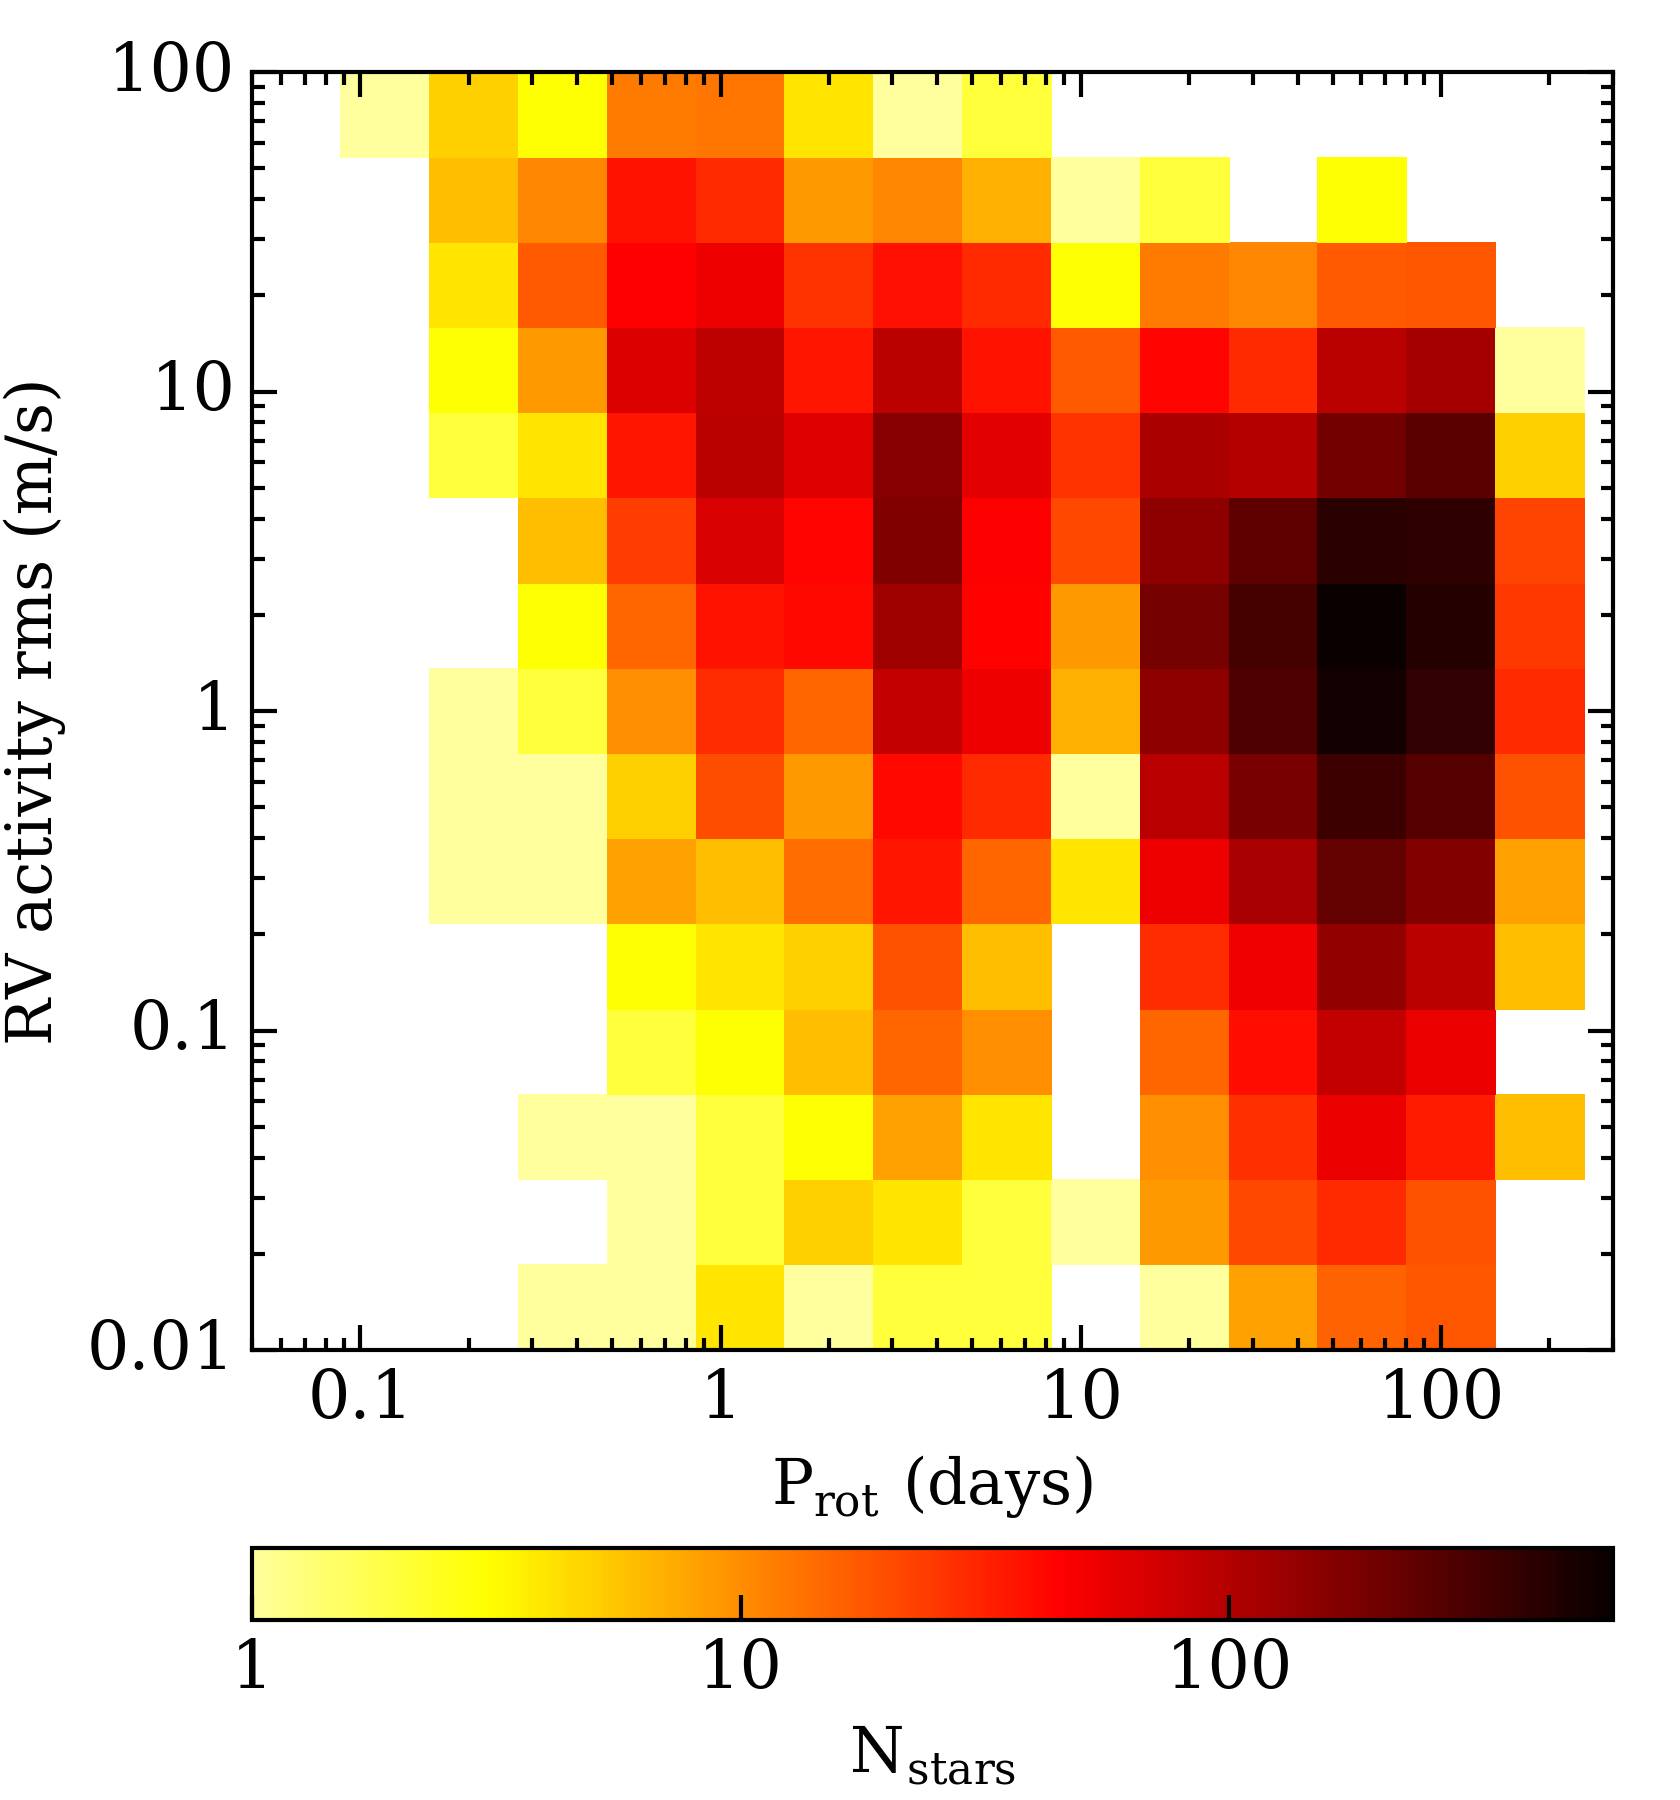
\includegraphics[width=0.6\hsize]{figures/rmsactivityProt_bkgd.png}%
  \hspace{-0.6\hsize}%
  \begin{ocg}{fig:curveoff}{fig:curveoff}{0}%
  \end{ocg}%
  \begin{ocg}{fig:curveon}{fig:curveon}{1}%
    
\includegraphics[width=0.6\hsize]{figures/rmsactivityProt_means.png}%
  \end{ocg}
  \hspace{-0.6\hsize}%
  \begin{ocg}{fig:Hoff}{fig:Hoff}{0}%
  \end{ocg}%
  \begin{ocg}{fig:Hon}{fig:Hon}{1}%
    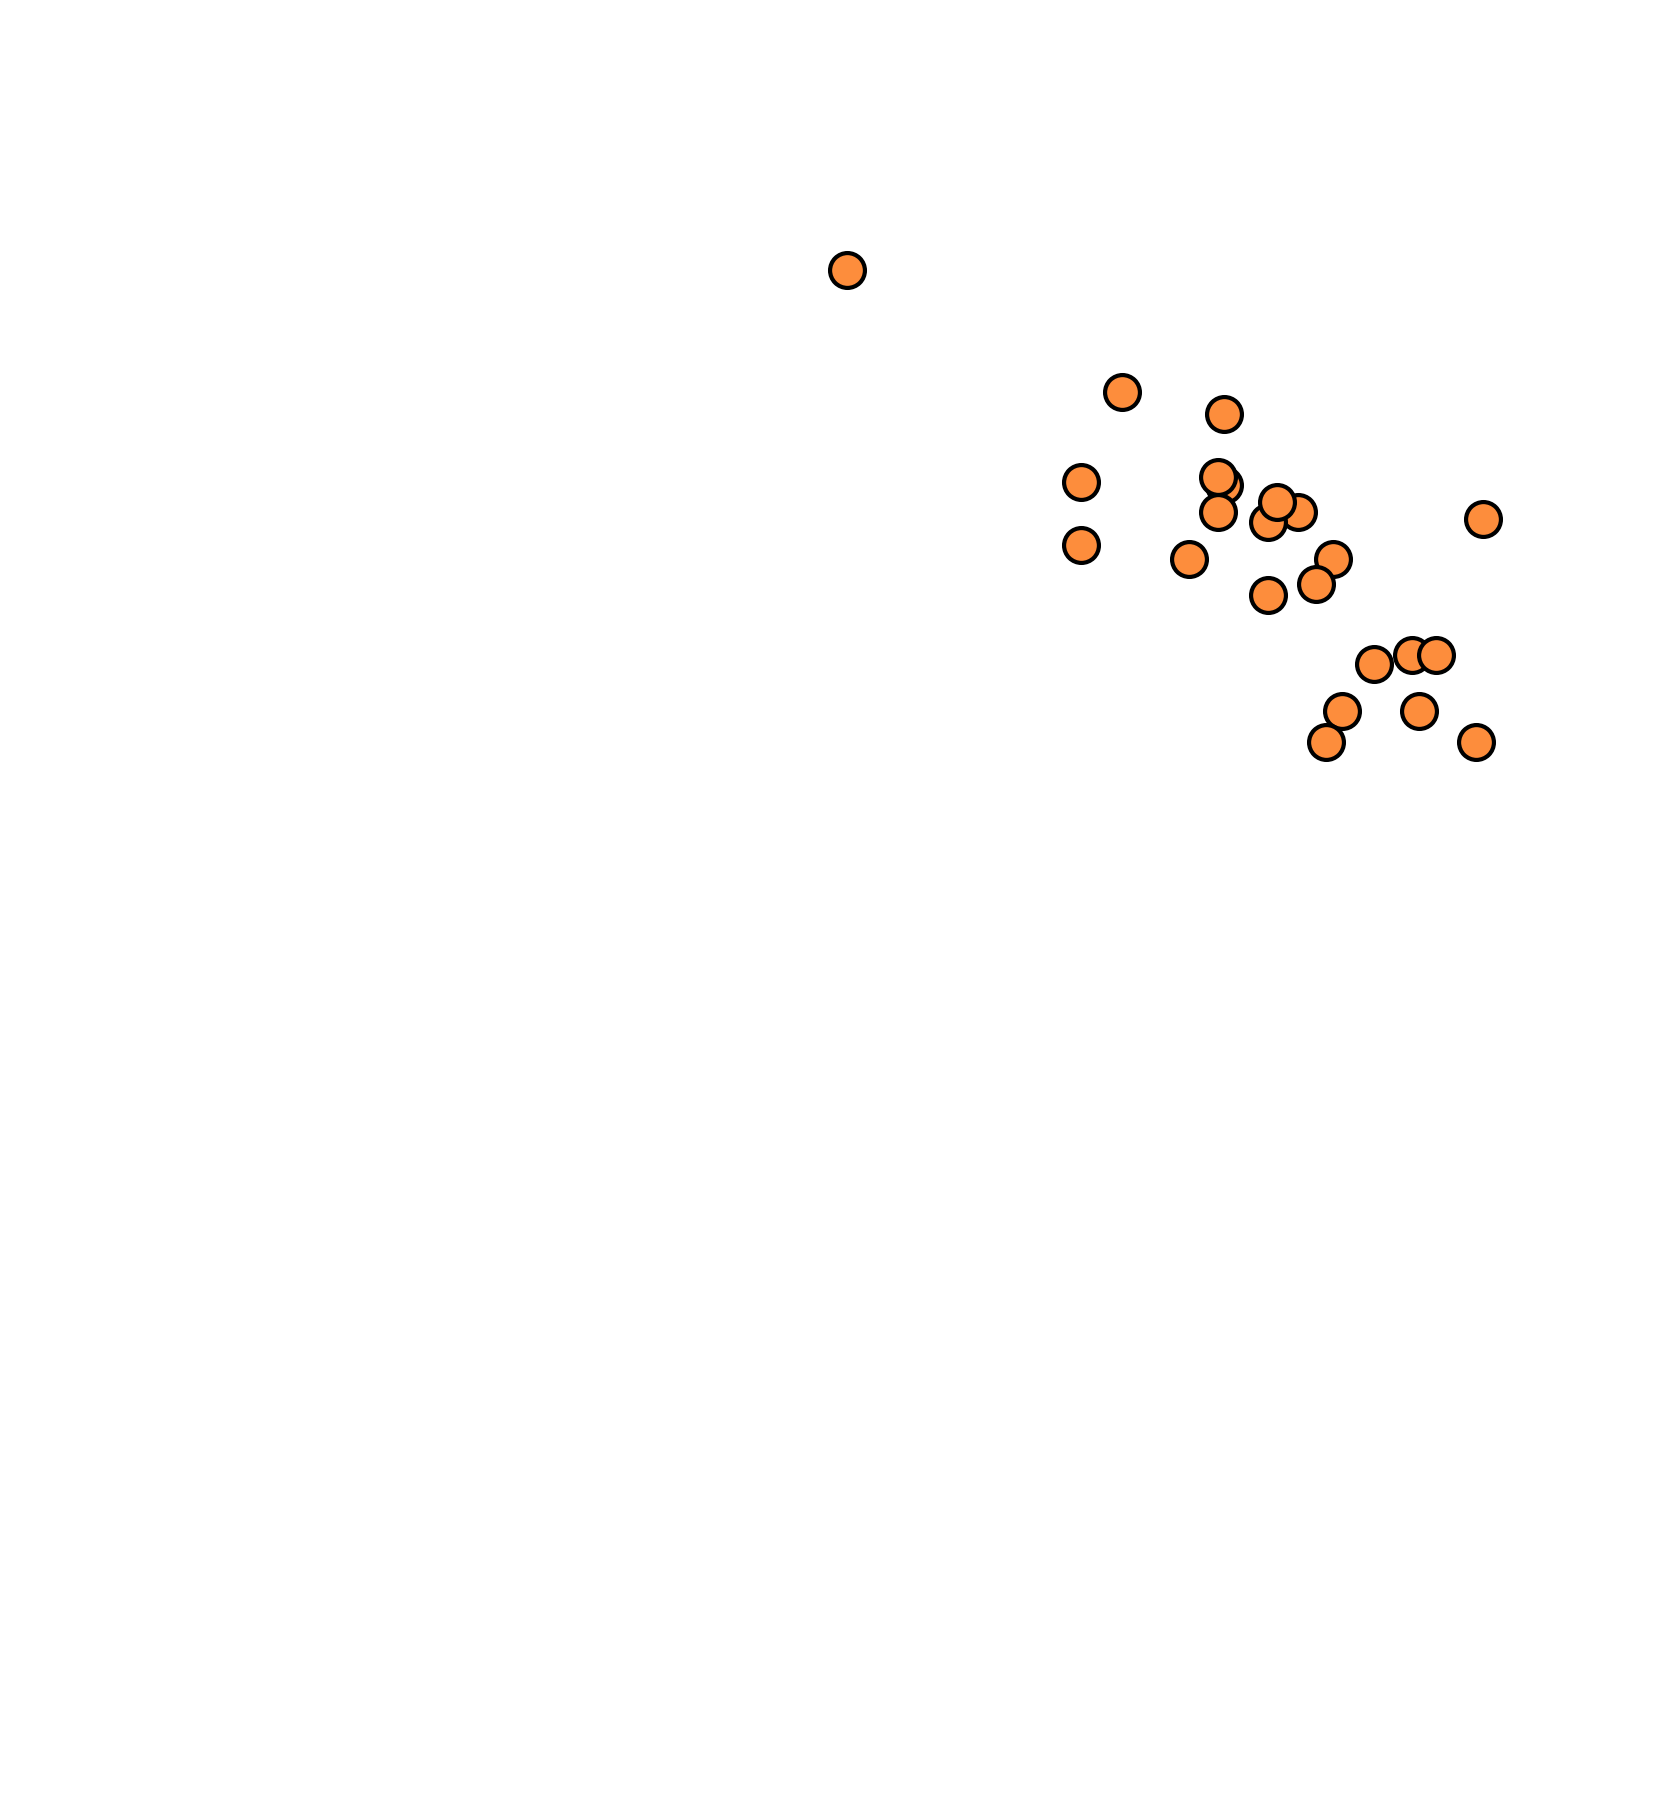
\includegraphics[width=0.6\hsize]{figures/rmsactivityProt_HARPS.png}%
  \end{ocg}
  \hspace{-0.6\hsize}%
  \caption[RV activity rms versus stellar rotation period.]
      {\small The RV activity rms as a function of stellar rotation period for stars in the simulated SLS-PS compared
    to a population of \ToggleLayer{fig:Hon,fig:Hoff}{\protect\cdbox{M dwarfs}} observed with the HARPS
    spectrograph. The \ToggleLayer{fig:curveon,fig:curveoff}{\protect\cdbox{\emph{dashed white curve}}} depicts the mean
    RV activity rms in each \prot{} bin.}
  \label{BSfig:activityrms}
\end{figure}


\subsubsection{Ignored sources of RV activity}
Various other minor sources of stellar activity in M dwarfs are ignored. These include radial pulsations which 
do not appear to persist with any significant amplitude within the interiors of M dwarfs
\citep{rodriguezlopez15}. Secondly, we disregard the effect of granulation whose amplitude scales
with the velocity of convective cells which itself decreases towards later spectral types
\citep{dumusque11a, meunier17}.
%Furthermore, the effect of granulation occurs on a characteristic timescale which is less than the
%typical integration time of the observations and is therefore marginalized over during the integration
%\citep{lovis05}.
Lastly, we ignore flares in our activity model because their distinctive
spectral signature allows them to be flagged and removed from the subsequent analysis
\citep{schmidt12, angladaescude16}.
However, the high occurrence rate of flaring events on many M dwarfs may prove costly when attempting to
construct large time-series of uncontaminated RVs.


\section{Simulated Survey} \label{BSsect:survey}
In this study we conduct a detailed Monte-Carlo (MC) simulation of the SLS-PS for the purpose of
predicting the SPIRou planet detection yield. To do so, we must construct a statistically significant
number of unique RV time-series for each of the 100 stars that we target throughout the simulated SLS-PS.
In practice we simulate 100 unique RV time-series for each star totalling $10^4$ realizations in the full
simulated SLS-PS. Each RV time-series contains unique signals from planets, which are sampled from their
known occurrence rates around early M dwarfs (see Sect.~\ref{BSsect:planetsample}), from physical models
of stellar activity (as described in Sect.~\ref{BSsect:activity}), and from instrumental noise.
Each contribution is sampled
in time using a unique window function spanning $\sim 300$ nights over $\sim 3$ years,
which represents the typical time baseline of observations for a single star
in accordance with the expected subset of SPIRou's time allocation that will be dedicated to the
discovery of new exoplanetary systems in the SLS-PS. We note however that at this time the exact number of available
nights dedicated to the SLS-PS, nor the duration of the full SLS-PS, have been established absolutely. In addition
to the RVs, we also derive various spectroscopic activity indicators arising from stellar activity
which are contemporaneous with the RVs. One such ancillary time-series is the full width at half maximum
(FWHM) of the cross-correlation function which will be used to
train non-parametric Gaussian process models of the RV activity based on its common covariance structure with
the FWHM (see Sect.~\ref{BSsect:GP}). SPIRou is also unique in that it simultaneously operates its spectroscopic and
polarimetry modes thus providing a contemporaneous diagnostic of the star's magnetic topology. Such time-series
may also
be used to model RV signals from magnetically ARs \citep{hebrard16} although we do not consider
such time-series in this study. \\

In each
simulated RV time-series we attempt to recover the injected planets to form an estimate of the expected
planet population that will be discovered with SPIRou. This is facilitated by the joint modelling of stellar
activity and planetary signals. This allows for the self-consistent characterization of each RV signal and the
detection of a subset of planets which are nominally hidden by their host star's intrinsic RV activity.


\subsection{Window Functions} \label{BSsect:wf}
In each MC realization, the unique window function $\mathbf{t}$ is the vector of length \nobs{} containing
the epochs of observation in barycentric julian dates (BJD). The window function describes the time sampling of
our time-series. To derive a set of window functions for each star in the SPIRou input catalog
we run a separate MC simulation of stellar observing sequences for all targets taking into account
when each
star is visible from CFHT on Maunakea with an airmass of $<2.5$ based on its celestial coordinates.
During every available night, all visible stars are observed up to two times,
each with an integration time required to achieve a
S/N per resolution element of 150---at the central $J$ band wavelength of 1.25 $\mu$m---with a minimum integration
time of 15 minutes. The imposed lower limit on the
integration time may also be necessary to mitigate the effects of granulation \citep{lovis05} which is
expected to be low on M dwarfs. 
Integration times required to achieve at least the target S/N are computed for
each star based using their $YJHK$ magnitudes. An overhead of 5 minutes is added to each
integration for guiding and setup purposes.
The output from these simulations is a set of window functions each pertaining to a star in the
SPIRou input catalog. Multiple MC simulations are run for various observing
sequences and thus provide unique window functions for the simulated SLS-PS. We then sample from
these window functions for the purpose of investigating
the sensitivity of our planet detection results to the exact form of the window function. \\

The available nights for observation with SPIRou are limited by two important considerations.
The first being the effect
of stochastic weather which limits the number of epochs in our derived window functions according to the
CFHT observatory's weather statistics. The second effect is somewhat unique to CFHT as the telescope hosts
a suite of instruments that do not operate simultaneously. In particular, the telescope's wide-field
optical imager requires dark-time to conduct its observations whereas the SPIRou spectro-polarimeter
does not. As such, we proceed with constructing SPIRou window functions that only include
non-dark-time observation and thus correspond to higher levels of lunar contamination. This represents
a worst case scenario for SPIRou as aliases from the window function will undoubtedly arise at periodicities
close to the cadence of the non-dark-time observing sequences. This cadence 
evolves with a period close to the period of the lunar cycle at $\sim 30$ days.
Because the SPIRou time sampling occurs in windows separated by $\sim 30$ days,
at that period and its first harmonic at 15 days, significant aliases in the Lomb-Scargle (LS)
periodogram \citep{scargle82}
of window function can arise as is shown in Fig.~\ref{BSfig:wfs}. The effect of these aliases are
detrimental to the detection of periodic planetary signals at these periods because
in the LS periodogram of the RVs, one cannot
distinguish a-priori between these periodic signals as a planet or as an alias of the time sampling
\citep{dawson10}.
This effect has already been shown to mimic planetary signals \citep[e.g.][]{rajpaul16} and is particularly
detrimental to finding HZ planets around $\sim$ M2-M4 dwarfs whose HZ span $\sim 30$ day orbital periods.
We quantify the magnitude of this aliasing effect on the SPIRou planet detection sensitivity in
Sect.~\ref{BSsect:sensitivity}. \\

\begin{figure}
  \centering
  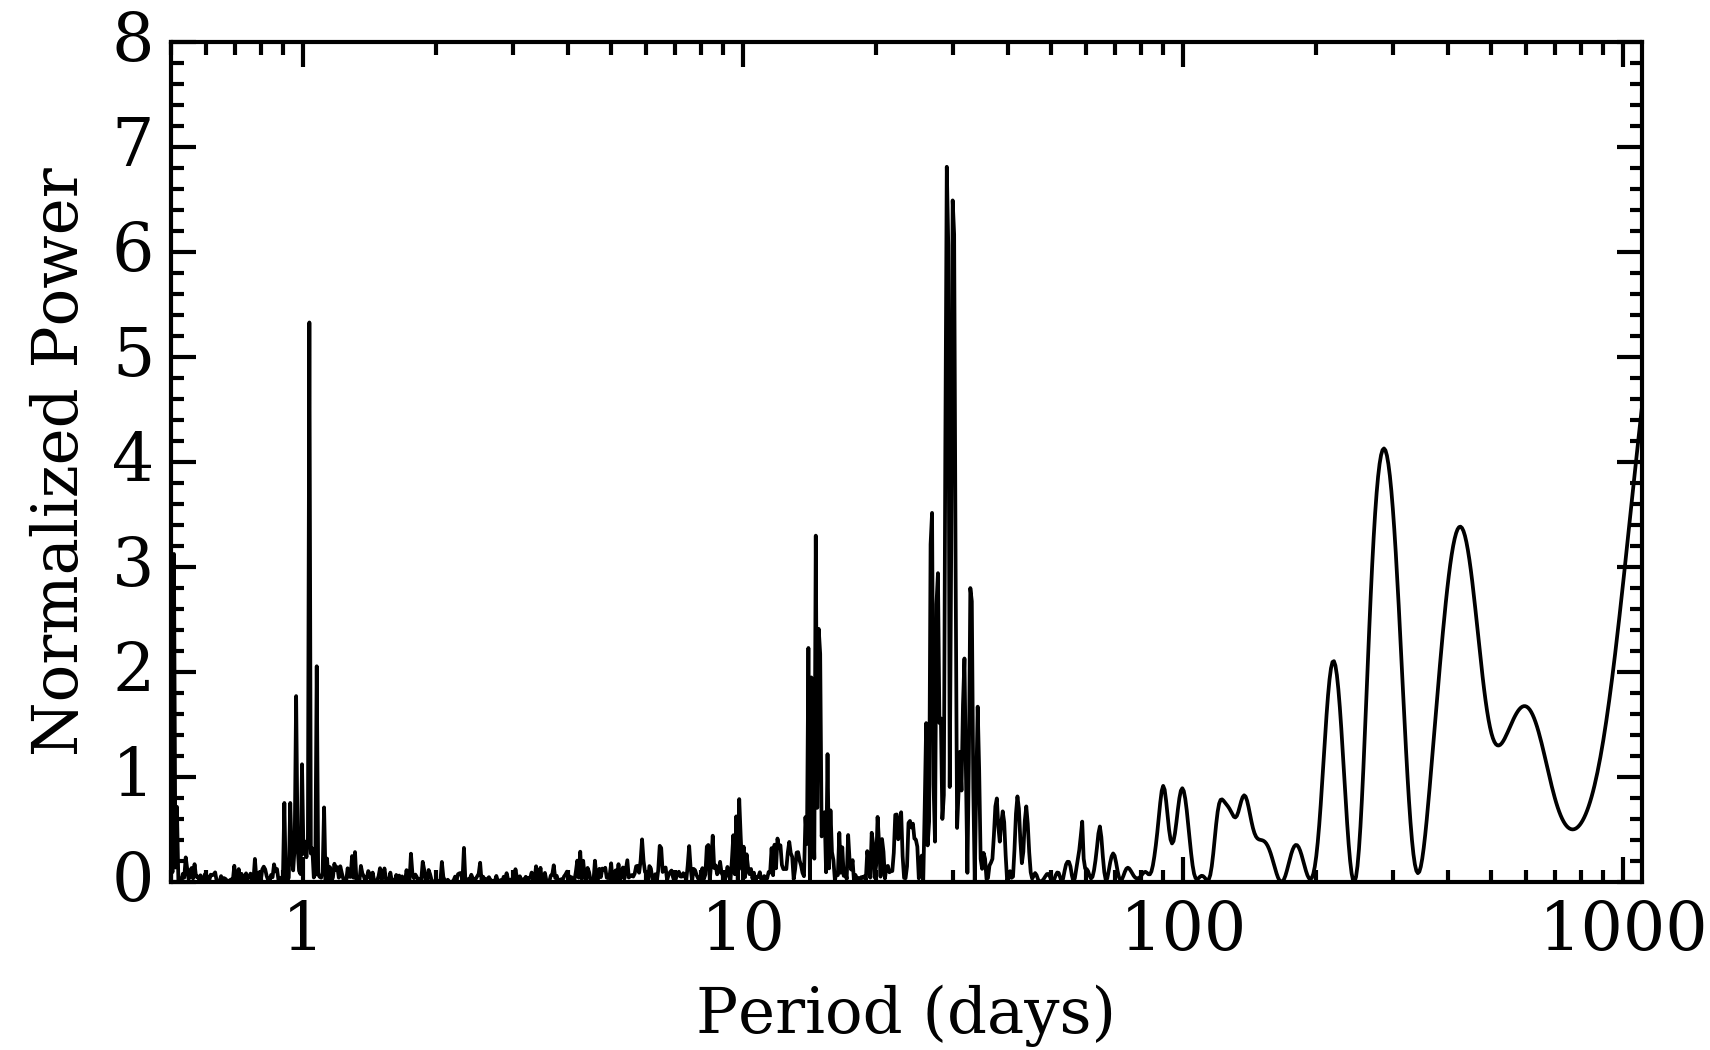
\includegraphics[width=0.8\hsize]{figures/WF_bkgd.png}%
  \hspace{-0.8\hsize}%
  \begin{ocg}{fig:Poff}{fig:Poff}{0}%
  \end{ocg}%
  \begin{ocg}{fig:Pon}{fig:Pon}{1}%
    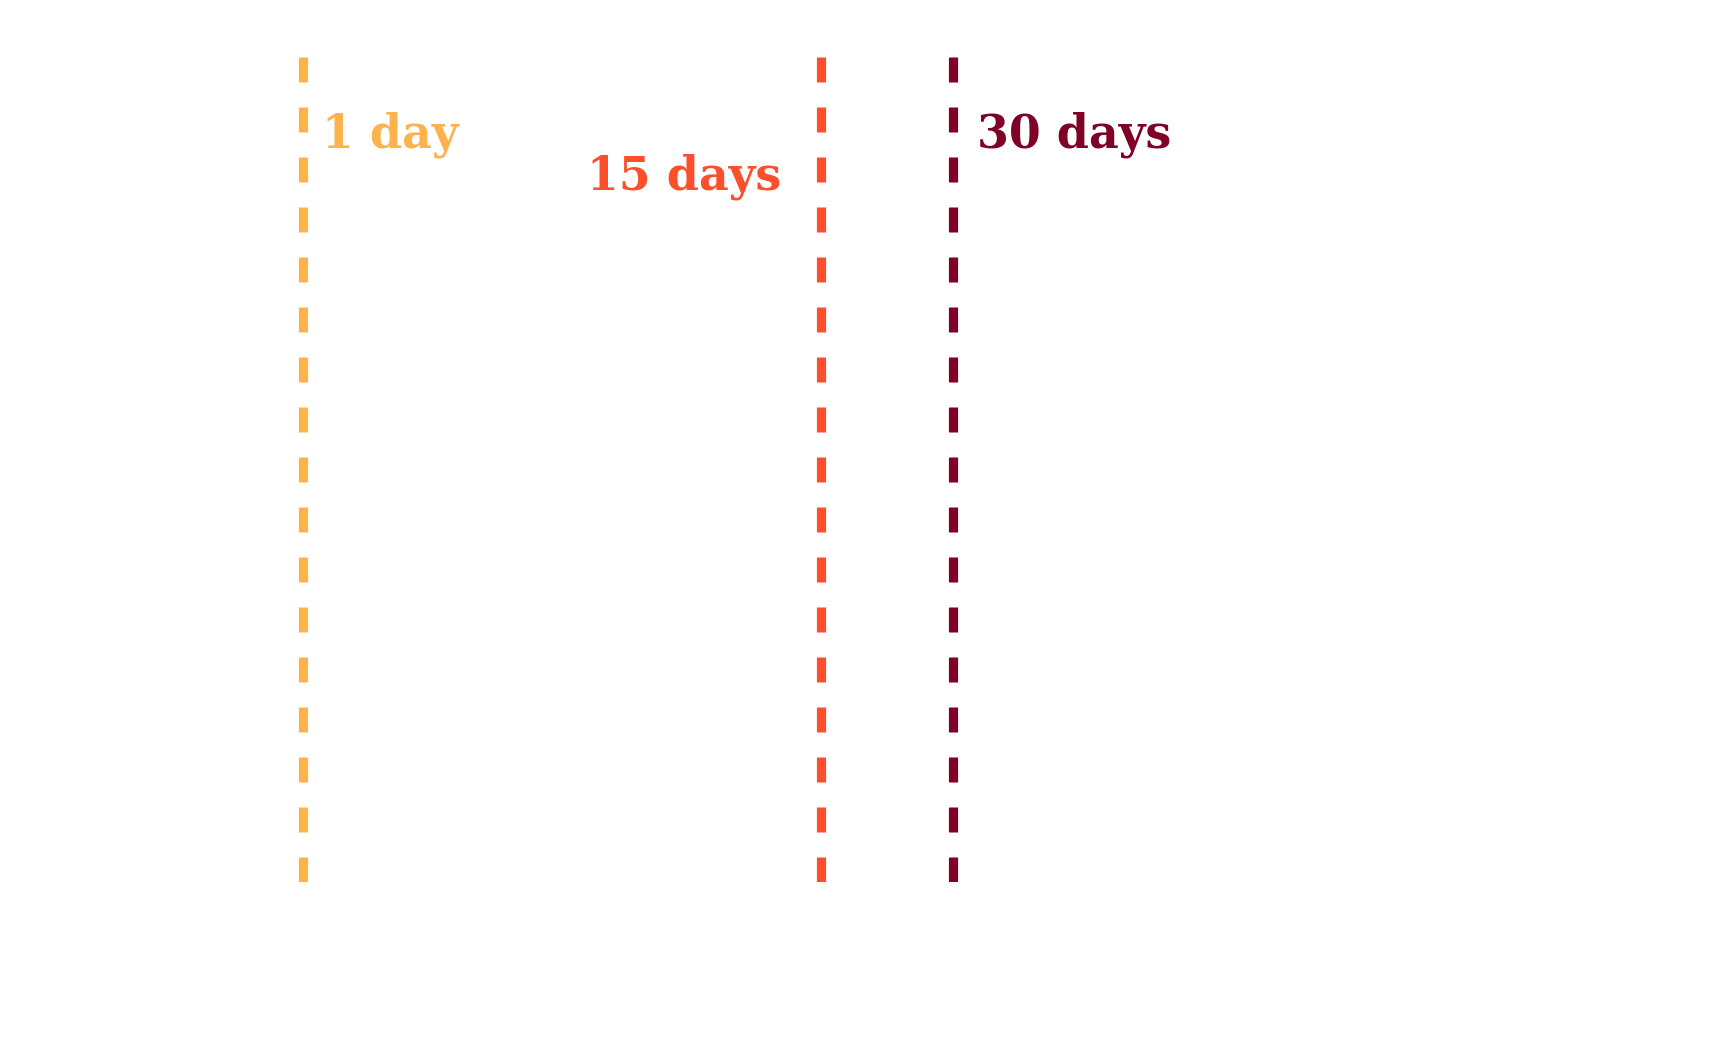
\includegraphics[width=0.8\hsize]{figures/WF_Ps.png}%
  \end{ocg}
  \hspace{-0.8\hsize}%
  \begin{ocg}{fig:FAPoff}{fig:FAPoff}{0}%
  \end{ocg}%
  \begin{ocg}{fig:FAPon}{fig:FAPon}{1}%
    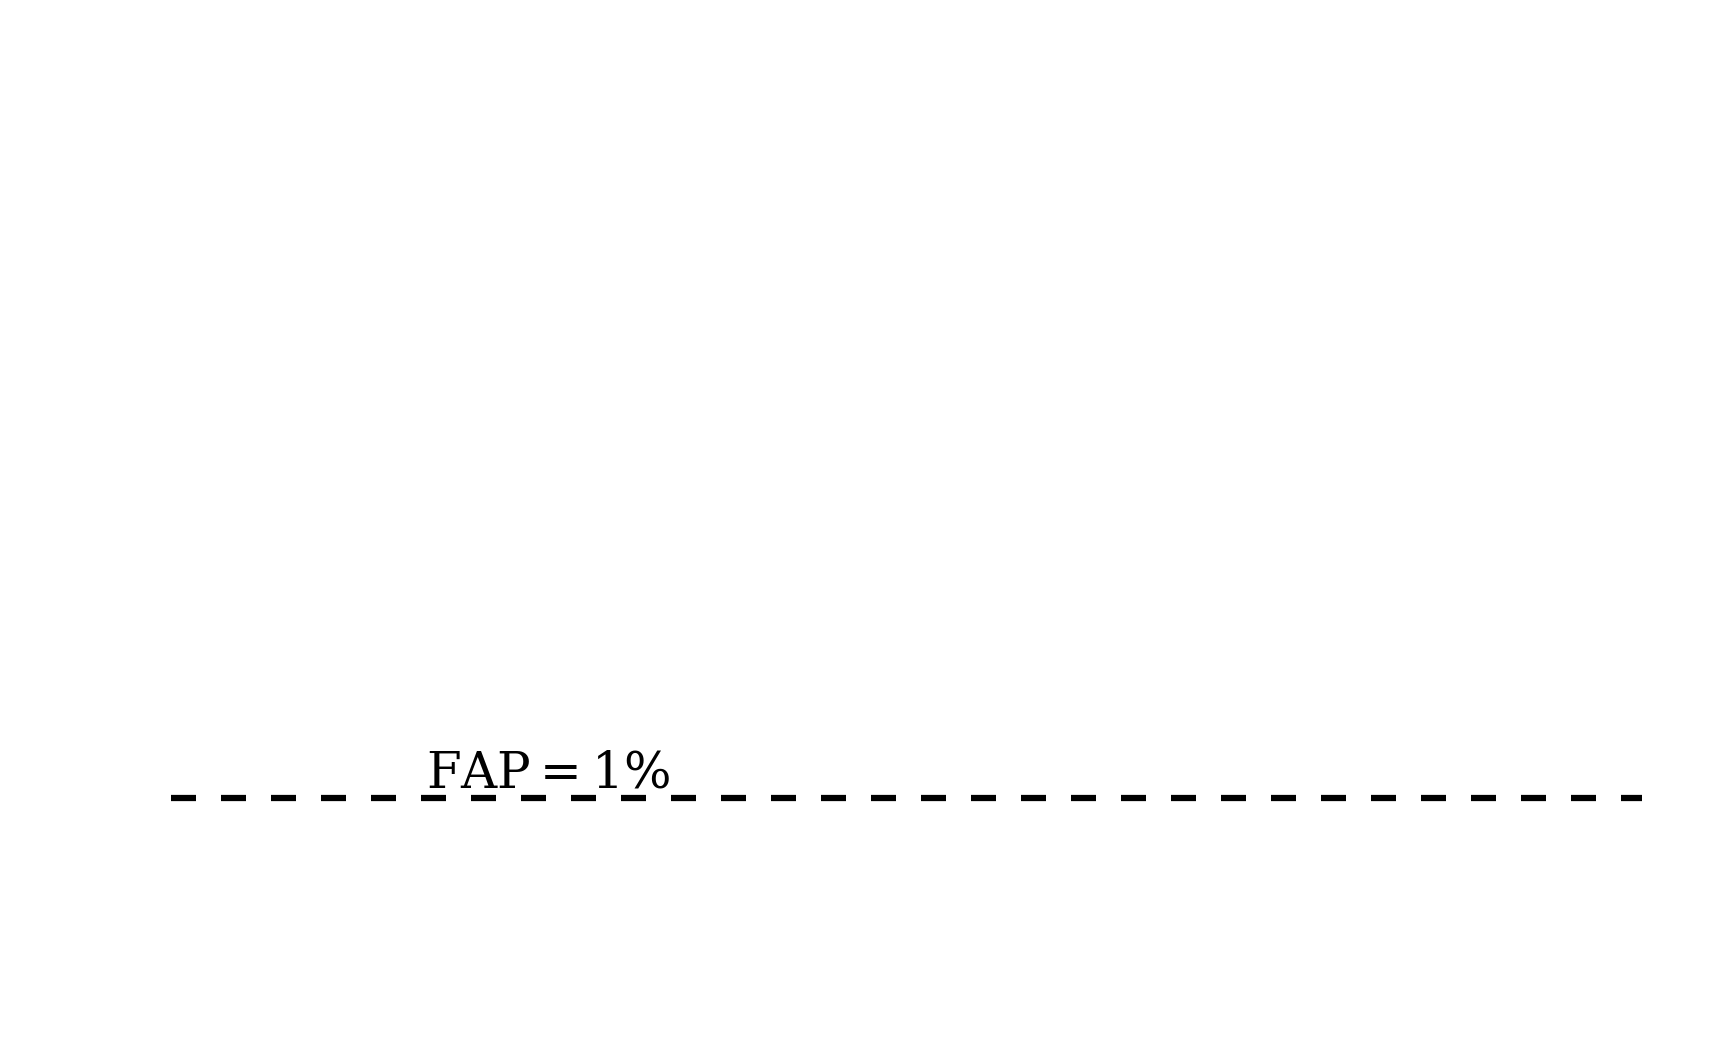
\includegraphics[width=0.8\hsize]{figures/WF_faps.png}%
  \end{ocg}
  \hspace{-0.8\hsize}%
  \caption[Lomb-Scargle periodogram of an expected SPIRou window function during the SLS-PS.]
    {\small Lomb-Scargle periodogram of an example window function from the simulated SLS-PS.
    The periodogram exhibits strong aliases from our time sampling at the periodicities
    highlighted by the 
    \ToggleLayer{fig:Pon,fig:Poff}{\protect\cdbox{\emph{vertical lines}}}. The power
    corresponding to a 1\% false alarm probability in the periodogram is highlighted by the  
    \ToggleLayer{fig:FAPon,fig:FAPoff}{\protect\cdbox{\emph{horizontal dashed line}}}.}
  \label{BSfig:wfs}
\end{figure}

For the purpose of performing accurate statistical inference of the SPIRou planet population
following the full SLS-PS (see Sect.~\ref{BSsect:occurrence}),
we attempt to split the total observing time evenly among the stars in the
SPIRou input catalog. Doing so, while taking into account stochastic weather and non-dark-time restrictions,
limits the size of our window functions over an a-priori 3 year long survey to an average of
198.1 RV measurements per star for 100 stars over $\sim 300$ nights. The variance in the number of RV
measurements per star is relatively small and ranges from 181-212. 
In the other versions of the SLS-PS containing either more or less stars than in our fiducial survey version
(see Sect.~\ref{BSsect:surveys}),
our MC calculations of the window functions consequently contain less and more RV measurements per star, respectively. \\

From preliminary simulations of the SLS-PS using 10 unique window functions per sampled planetary system per star,
we found that the net planet detection results are largely independent of the exact window function used. Note that
all sampled window functions contained the same restrictions discussed previously but do not include the exact
same epochs of observation for each star. Explicitly,
the SPIRou planet yield was found to vary by only $\sim 1$\% across the various window functions used.
This dispersion is much
less than the uncertainties on the resulting estimates of the SPIRou planet yield due solely to uncertainties in
the input planet occurrence rates. Therefore we conclude that using multiple window functions for each planetary
system in our simulated
SLS-PS is an unnecessary computational expense that can be mitigated by considering a single window function
per planetary system and not significantly affect the results of our study. However each unique window function considered
was still assumed to be restricted to non-dark-time observations thus preserving the aliasing affect on planets with
orbital periods of $\sim 30$ days.


\subsection{Radial Velocity Time-Series Construction} \label{BSsect:timeseries}
In each MC realization, 
the RV contribution from $N_p$ injected planets in the simulated planetary system (see Sect.~\ref{BSsect:planetsample})
is calculated via the superposition of $N_p$ keplerian orbital solutions. Each keplerian RV$_{kep}$ is parameterized by
the planet's orbital period $P$, time of inferior conjunction $T_0$, orbital eccentricity $e$,
argument of periastron $\omega$, and RV semi-amplitude $K$ according to

\begin{equation}
 \text{RV}_{kep}(t) = K [\cos{(\nu(t) +\omega)} + e \cos{\omega}],
\end{equation}

\noindent where $\nu(t)$ is the true anomaly and is computed by solving Kepler's equation
and the eccentric anomaly as a function of time $t$ contained in the window function
$\mathbf{t}$. The RV semi-amplitude $K$ is computed from the planet's minimum mass
\msini{,} the stellar mass $M_s$, $P$, and $e$ using the standard formula

\begin{equation}
  K = 1.05 \text{ m s}^{-1} \left(\frac{m_p\sin{i}}{2\text{ M}_{\oplus}} \right)
  \left( \frac{P}{20 \text{ days}} \right)^{-1/3} 
  \left( \frac{M_s}{0.3 \text{ M}_{\odot}} \right)^{-2/3}
  \frac{1}{\sqrt{1-e^2}}.
\end{equation}

The keplerian RV approximation
is valid in all single-planet systems and the majority of multi-planet systems considered
and is best motivated by its ability to negate the
need to perform costly numerical integrations of each sampled planetary system. However, we note that
this approximation naturally excludes certain dynamical effects in multi-planet systems such as planet-planet
interactions and mean-motion resonances which can affect the planet-induced periodicities within
the RV time-series and therefore also affect our ability to detect those planets.
Although the former effect is not accounted for in our simulated time-series, its amplitude in real
systems is typically small compared to the RV measurement uncertainty as a result of dynamical restrictions
on multi-planetary systems making tightly-packed systems less stable over long time-scales and therefore
rarely seen in nature.
The significance of the latter effect is also expected to be small given the dearth of 
multi-planet systems at low-order period ratio commensurabilities \citep{lissauer11, fabrycky14}. \\

All RV components are evaluated at $\mathbf{t}$ and contain the additive i) RV activity RV$_{act}$ derived from 
physical models (see Sect.~\ref{BSsect:activity}) ii) $N_p$ keplerian models, and iii) a white noise term with an rms equal
to the median RV measurement uncertainty $\sigma_{\text{RV}}$ expected for the host star. Each star's value of
$\sigma_{\text{RV}}$ is calculated using the nIR RV
information content calculations from \cite{figueira16} corrected using the empirical spectra from \cite{artigau18}.
We use the results from the condition 3 in \cite{figueira16} to estimate $\sigma_{\text{RV}}$:
the photon-noise contribution to the spectrum
being amplified by the limited spectral window due to atmospheric telluric transmission.
The information content calculations for each star are computed using SPIRou's spectral resolution,
spectral coverage, and the expected S/N per resolution element obtained during an integration of the star. \\

The RV activity model contains additive contributions from the flux effect, the suppression of convective blueshift,
and Zeeman broadening from ARs. The complete RV model is therefore

\begin{equation}
  \text{RV}_{model}(t) = \text{RV}_{act}(t) + \sum_{i=1}^{N_p} \text{RV}_{kep,i}(t) + \mathcal{N}(0,\sigma_{\text{RV}}).
\end{equation}

\noindent The RV measurement uncertainties pertaining to each measured RV is contained in the vector
$\boldsymbol{\sigma_{\text{RV}}}$ and is modified from the scalar value of $\sigma_{\text{RV}}$
based on the variable absorption by terrestrial
water vapor. The water vapor correction at each epoch in $\mathbf{t}$ is the product of the airmass and the zenith
water column from the well-documented CFHT observing condition statistics throughout the calendar year. 
The distribution of median $\sigma_{\text{RV}}$ in our MC simulation for our full
stellar sample is shown in Fig.~\ref{BSfig:sigmaRV} as a function
of the stellar $J$ band magnitude and \vsini{.} A noise floor is imposed at the expected long-term RV precision limit
of SPIRou at 1 \mps{.} This results in a median
$\sigma_{\text{RV}}=1.52$ \mps{.} The maximum $\sigma_{\text{RV}}$ is 6.58 \mps{.} 
Not depicted in Fig.~\ref{BSfig:sigmaRV} is the dependence of
$\sigma_{\text{RV}}$ on spectral type as the RV measurement uncertainty tends to decrease towards later spectral types
due to the increased number of available spectral features and corresponding increase in RV information content. \\

\begin{figure}
  \centering
  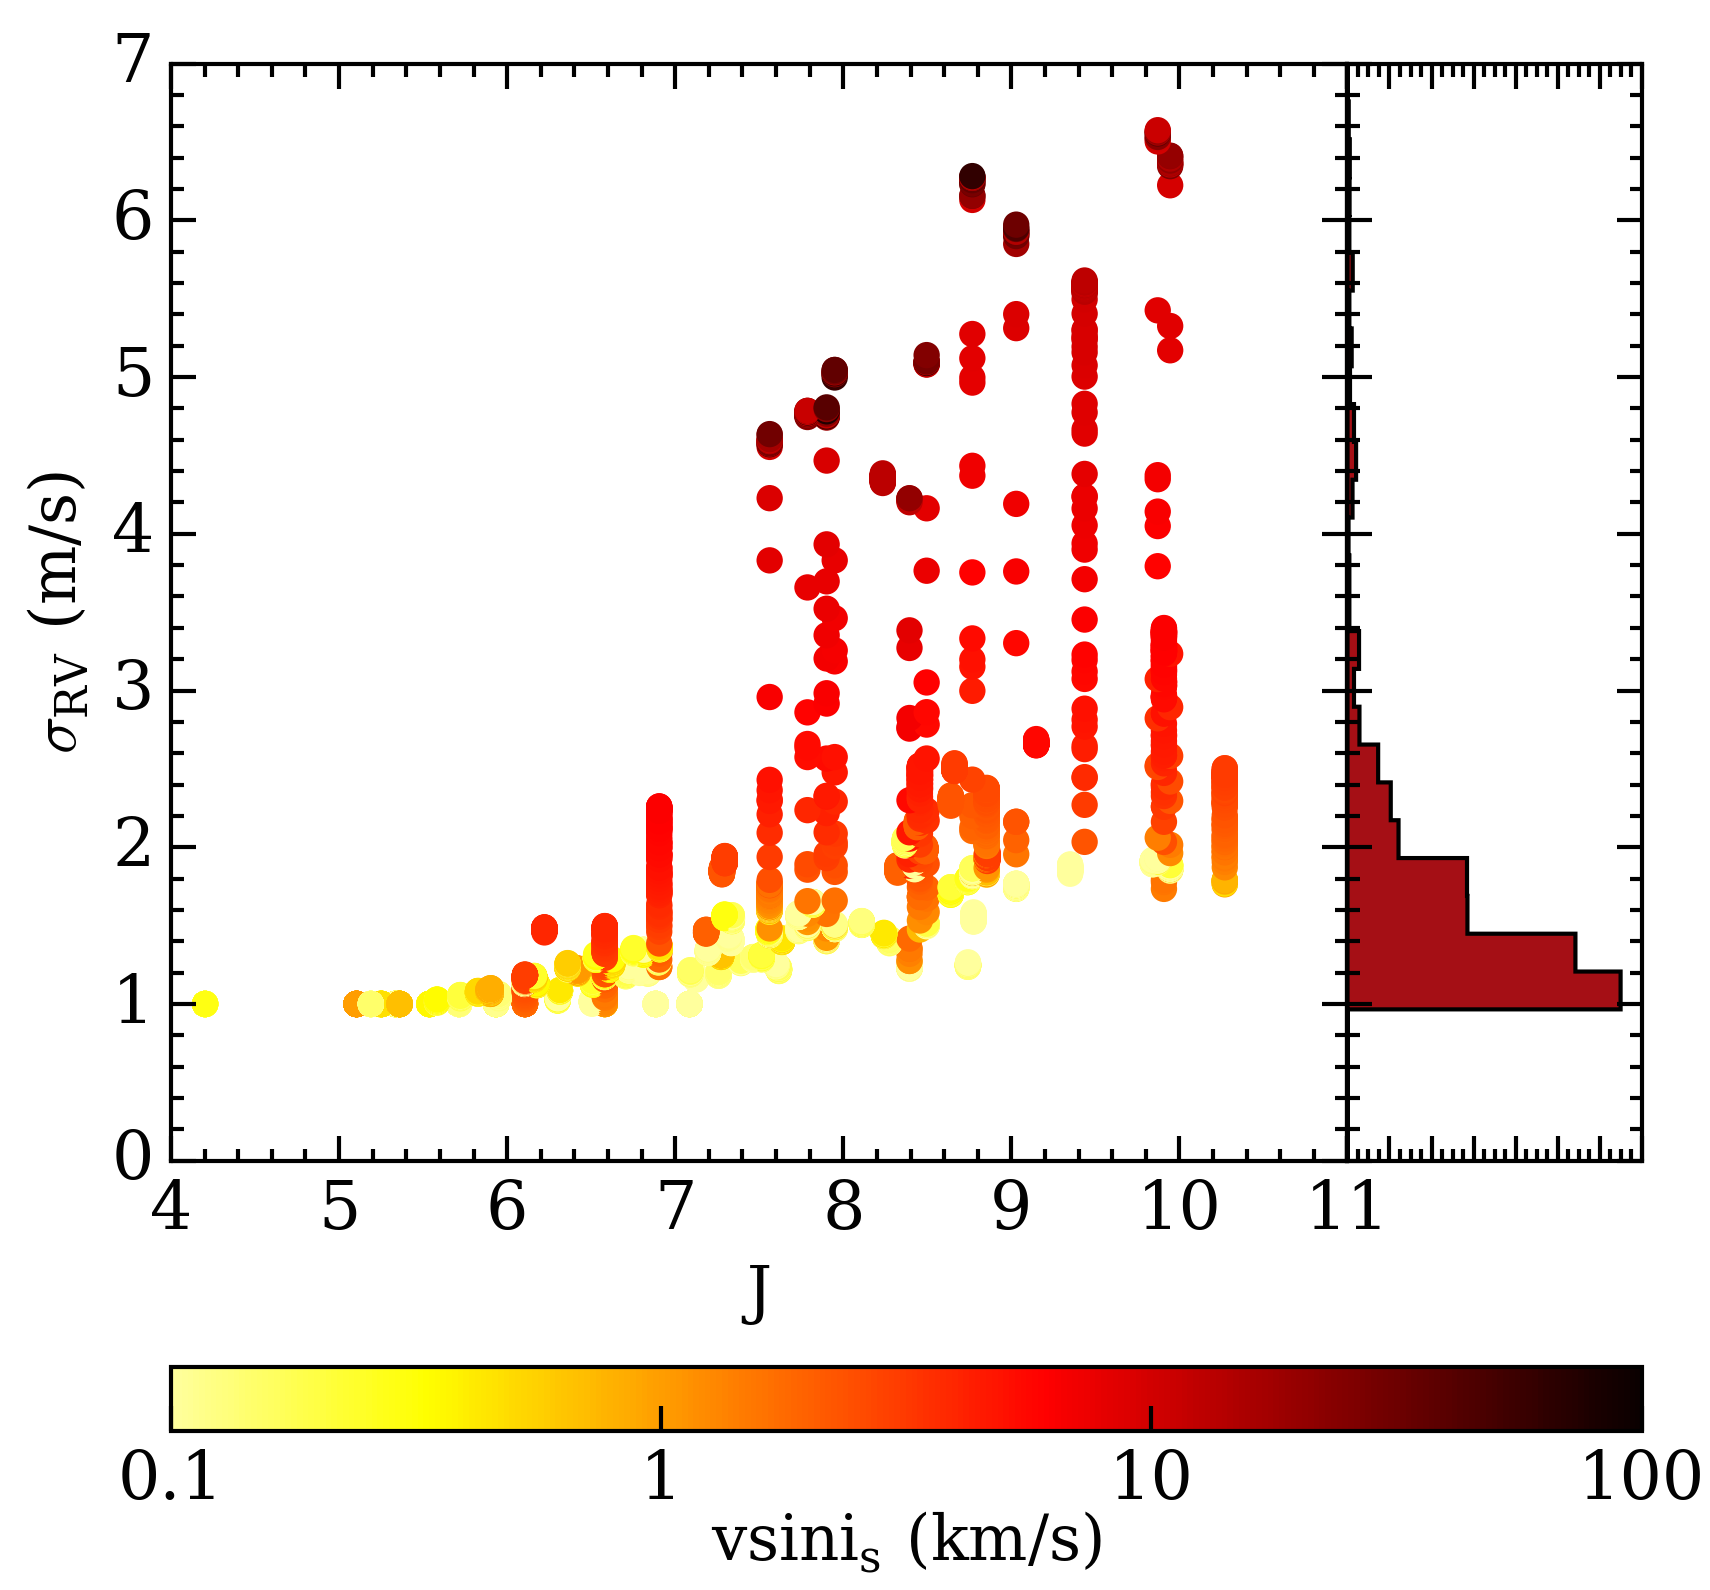
\includegraphics[width=0.6\hsize]{figures/sigmaRV.png}%
  \caption[RV measurement uncertainty versus $J$-band magnitude and \vsini{.}]
      {\small The median RV measurement uncertainty in each simulated RV time-series $\sigma_{\text{RV}}$
    as a function of the star's $J$-band magnitude and projected stellar rotation velocity \vsini{.} A noise floor is
    imposed at 1 \mps{.} The histogram shown in the right panel is in linear units.}
  \label{BSfig:sigmaRV}
\end{figure}

Similarly to the construction of the RV activity time-series at the epochs in $\mathbf{t}$, the FWHM and BIS
ancillary times-series are constructed from our \texttt{SOAP 2.0} simulations (see Sect.~\ref{BSsect:soap}) 
at the same epochs as the RVs. These contemporaneous time-series will be used in Sect.~\ref{BSsect:GP} to
model the RV activity and help to detect underlying planetary signals.


\section{Planet Sample} \label{BSsect:planetsample}
\subsection{Planet Sample from known Occurrence rates}
In each MC realization we populate the simulated M dwarf planetary system with planets according to
their known occurrence rates from the \emph{Kepler} transit survey \citep{dressing15a}. In practice
we sample from a grid in orbital period $P$ and planetary radius $r_p$
according to the measured planetary occurrence rate at each point in the parameter space $f(P,r_p)$.
We assume that each point in the parameter space is
uncorrelated aside the dynamical stability constraints that we will apply to closely packed systems 
(see Sect~\ref{BSsect:dynam}). \\

The occurrence rates $f(P,r_p)$ (or equivalently $f$) from which we sample planets have
associated asymmetric uncertainties which are derived from data-driven posterior distributions
rather than from analytically-defined distributions which are more easily sampled from. \cite{dressing15a}
only present the modes and $1\sigma$ dispersions of their $f$ posteriors which is insufficient information
to reconstruct their $f$ posteriors in each $P$ and $r_p$ bin. To account for their reported uncertainties on
$f$ we must assume a functional form of the $f$ posteriors.
For each bin in $P$ and $r_p$ we sample planets with a probability drawn
from $\mathcal{N}(\mu, \bar{\sigma})$ where $\mu$ is the most likely value
of $f$ and $\bar{\sigma} = \text{mean}(\sigma_{\text{upper}},\sigma_{\text{lower}})$ where
$\sigma_{\text{upper}}$ and $\sigma_{\text{lower}}$ represent the asymmetric uncertainties on $f$.
The values of $\mu$, $\sigma_{\text{upper}}$, and $\sigma_{\text{lower}}$ are provided in \cite{dressing15a}
(see their Table 4) for all $P$ and $r_p$ bins for which $f>0$. For bins in which $f$ is consistent with zero,
we set $\mu=0$ and $\bar{\sigma}$ equal to the $1\sigma$ upper limit on $f$. For bins in
which $f$ is completely unconstrained as a result of a low detection sensitivity, we assume that $f(P,r_p)$ 
evolves smoothly such that we can extrapolate the values of $f$ from surrounding
bins with constraints in order to estimate the values of $f$ where it is unconstrained by the data
(e.g. $r_p \leq 1$ R$_{\oplus}$ and $P \geq 18.2$ days).
The extrapolated values are treated as $1\sigma$ upper limits and $\mu$ is set to zero such that when
integrating the most likely values of
$f(P,r_p)$ over the range of periods and planet radii considered by \citealt{dressing15a} ($P \in [0.5,200]$ days,
$r_p \in [.5,4]$ R$_{\oplus}$) we recover their cumulative
planet occurrence rate of $2.5 \pm 0.2$ planets per M dwarf. However our dynamical stability constraints will
reject a subset of sampled planetary systems thus effectively reducing the cumulative planet occurrence rate to
$<2.5$. \\

The dispersion in mutual inclinations among planets in multi-planet 
systems is related to the dispersion in eccentricities by $\langle i^2 \rangle \sim \langle e^2 \rangle /4$ 
\citep{stewart00, quillen07} with the mean orbital inclination 
to the plane of the sky $i$ being set to the value of $i_s$ obtained for the host star (i.e. from a geometrical
distribution). Although the distribution of spin--orbit angles for small planets around
M dwarfs has yet to be established, the observed low dispersion in orbital eccentricities \citep{vaneylen15}
and mutual inclinations \citep{figueira12, fabrycky14} in these types of planetary systems suggests that
they are dynamically cold. If this is indeed the case then the normal vector
to the mean planetary orbital plane is expected to be close to parallel to the stellar spin axis; $i \approx i_s$.
In each planetary system we sample each planet's orbital eccentricity $e$ from the $\beta$ probability
distribution describing the high detection significance sample of RV planets reported in \cite{cloutier15}
\citep[see also ][]{kipping13}. 

\subsection{Modifications to the Planet Sample} \label{BSsect:dynam}
Our adopted approach for sampling planetary systems is accompanied by four important caveats. \\

\emph{Converting planet radii to masses}. Firstly, the Kepler-derived $f$ directly samples
planetary radii whereas RV surveys are only sensitive to the planetary minimum
masses. Therefore an assumption must be made regarding the 
planetary mass-radius relation required to convert the sampled planetary radii into masses.
We opt for the following empirical mass-radius relation derived in \cite{weiss14} from an unbiased
sample of known transiting planets:

\begin{equation}
  \frac{m_p}{\text{M}_{\oplus}} =
  \begin{cases}
    0.440 \left( \frac{r_p}{\text{R}_{\oplus}} \right)^3 + 0.614 \left( \frac{r_p}{\text{ R}_{\oplus}} \right)^4, &
    r_p < 1.5 \text{ R}_{\oplus} \\
    2.69 \left( \frac{r_p}{\text{R}_{\oplus}} \right)^{0.93}, & r_p \ge 1.5 \text{ R}_{\oplus}. \\
  \end{cases}
 \label{BSeq:mr}
\end{equation}

\noindent This piece-wise mass-radius relation distinguishes between small rocky planets with
$r_p < 1.5$ R$_{\oplus}$ and larger gaseous planets \citep[e.g.][]{rogers15, dressing15b, fulton17}. The
intrinsic dispersion about the \emph{mean} mass-radius relation in Eq.~\ref{BSeq:mr} has characteristic
rms values of

\begin{equation}
  \sigma_{\text{rms}} =
  \begin{cases}
    2.7 \text{ M}_{\oplus}, & r_p < 1.5 \text{ R}_{\oplus} \\
    4.7 \text{ M}_{\oplus}, & r_p \ge 1.5 \text{ R}_{\oplus}. \\
  \end{cases}
  \label{BSeq:mrscat}
\end{equation}

\noindent To include this intrinsic dispersion in our sampled planet population, for each sampled $r_p$
we compute the mean $m_p$ using Eq.~\ref{BSeq:mr} and add an additional offset drawn from
$\mathcal{N}(0,\sigma_{\text{rms}})$
where the value of $\sigma_{\text{rms}}$ is given by Eq.~\ref{BSeq:mrscat}. We reject planets with unphysical
negative masses
which naturally biases our sample to larger planet masses than are predicted by the \emph{mean} mass-radius
relation. We then apply a unique correction factor to each radius bin $r_p$ with a width of 0.2 R$_{\oplus}$
such that we recover the \emph{mean} mass-radius relation given in Eq.~\ref{BSeq:mr} in our final planet sample.
Our Kepler-derived planet sample in the mass-radius plane is shown in Fig.~\ref{BSfig:mr} along with the 
\emph{mean} mass-radius relation. Over-plotted are the mean planet masses in each $r_p$ bin demonstrating the
accuracy of our unique correction factors used to recover the mean mass-radius relation. Note the large
uncertainties in the mean planet masses resulting from the large dispersion observed in the empirical mass-radius
relation \citep{weiss14}. \\

\begin{figure}
  \centering
  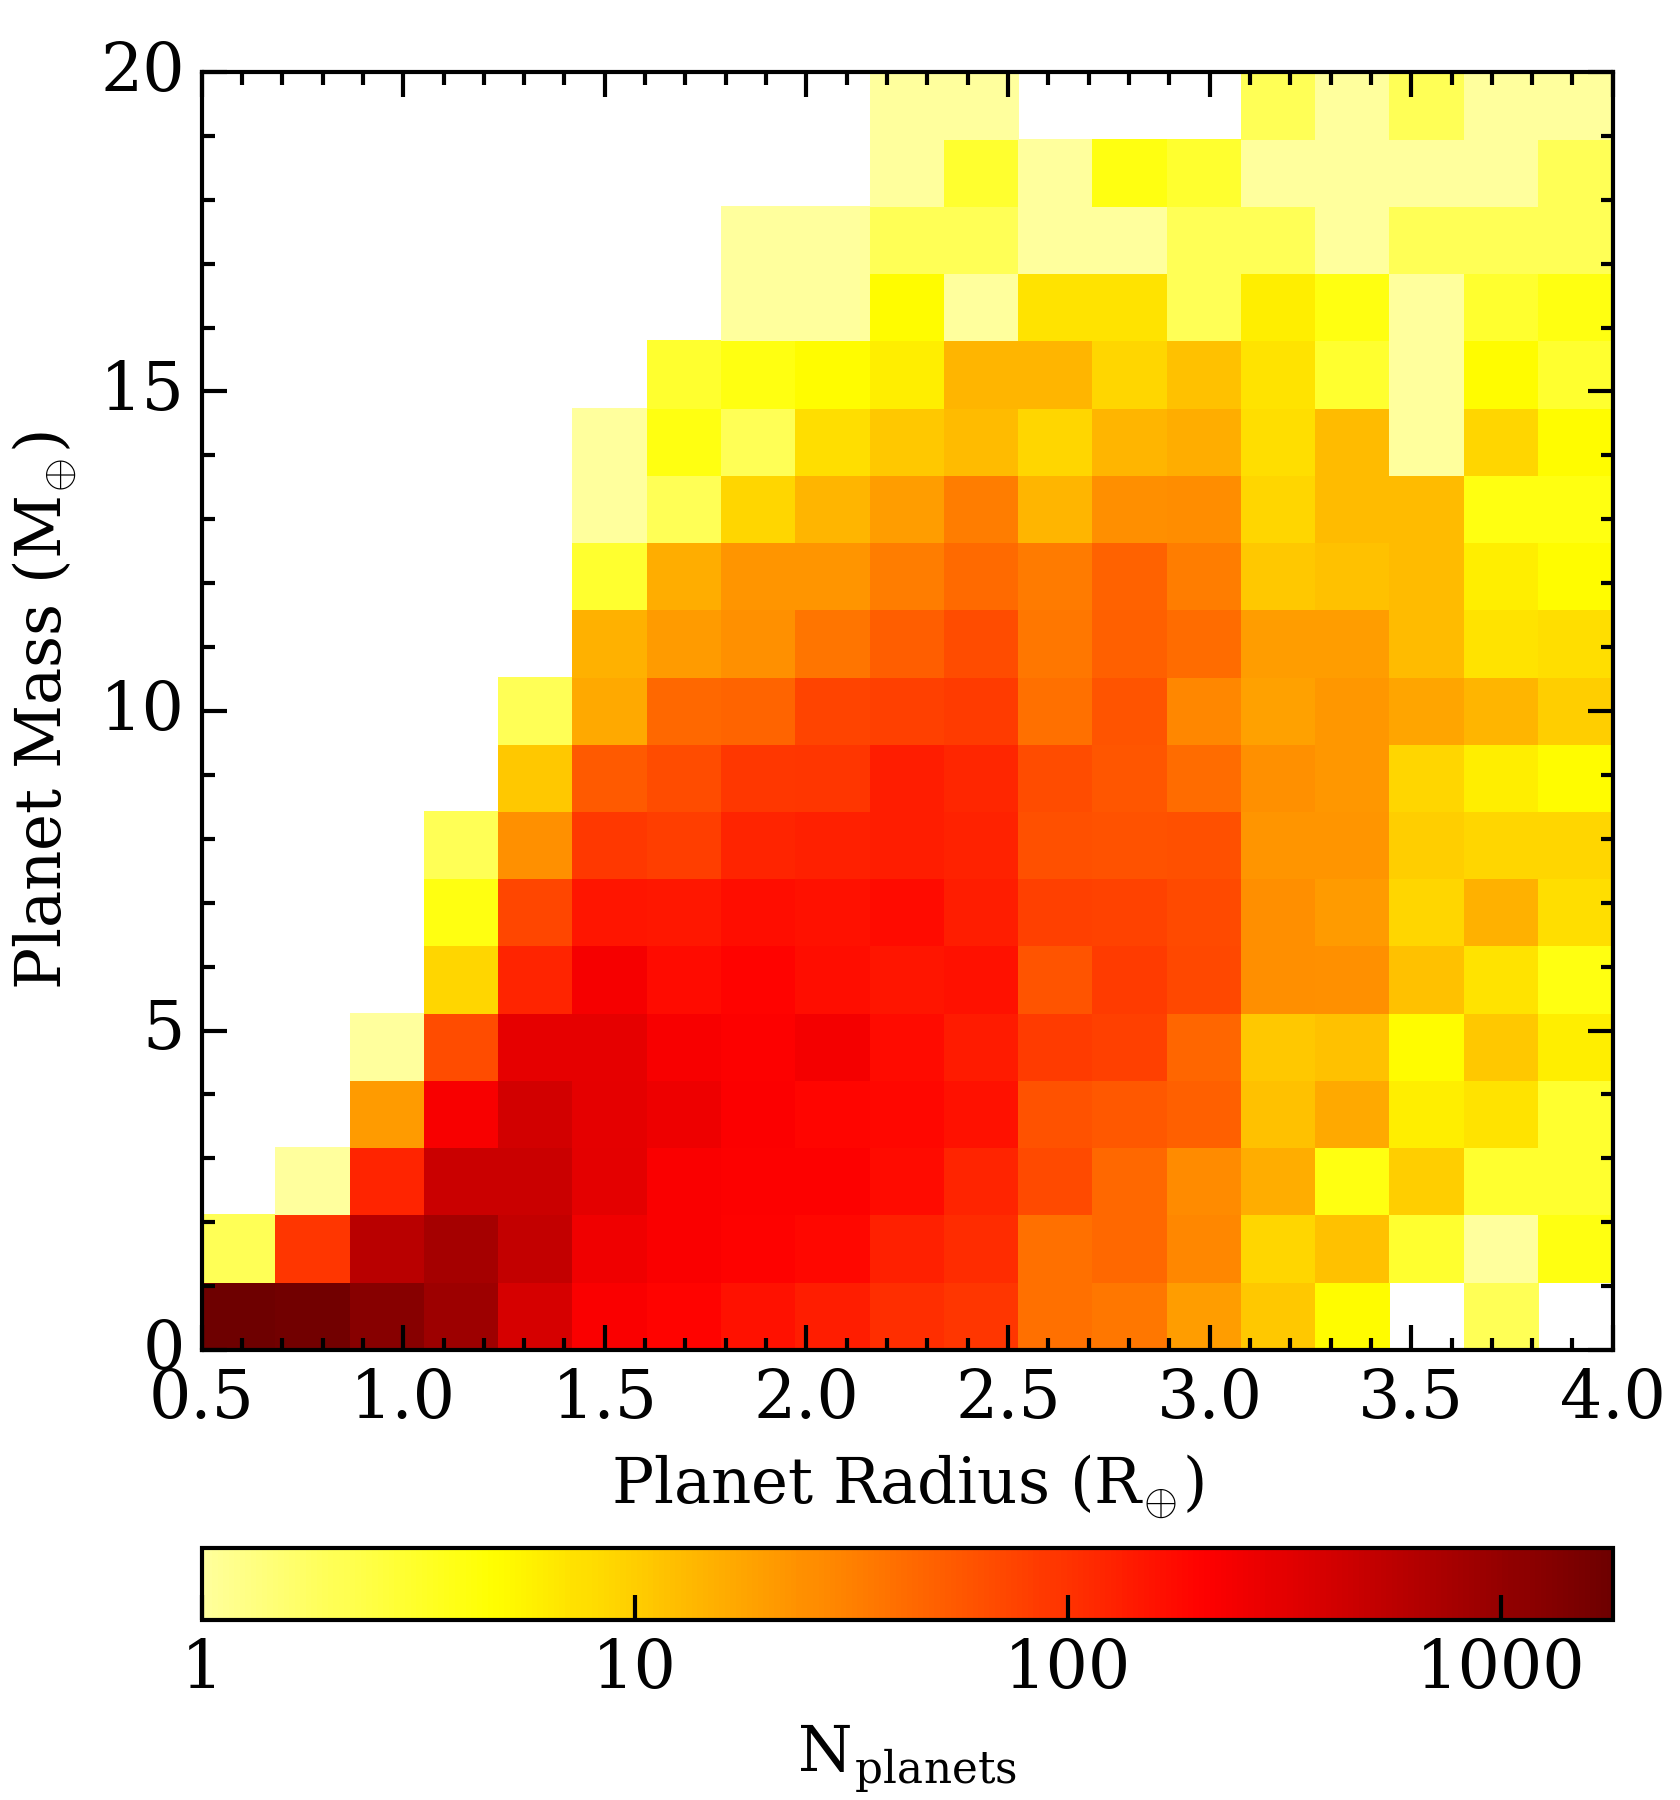
\includegraphics[width=0.6\hsize]{figures/MRscatter_bkgd.png}%
  \hspace{-0.6\hsize}%
  \begin{ocg}{fig:curveoff}{fig:curveoff}{0}%
  \end{ocg}%
  \begin{ocg}{fig:curveon}{fig:curveon}{1}%
    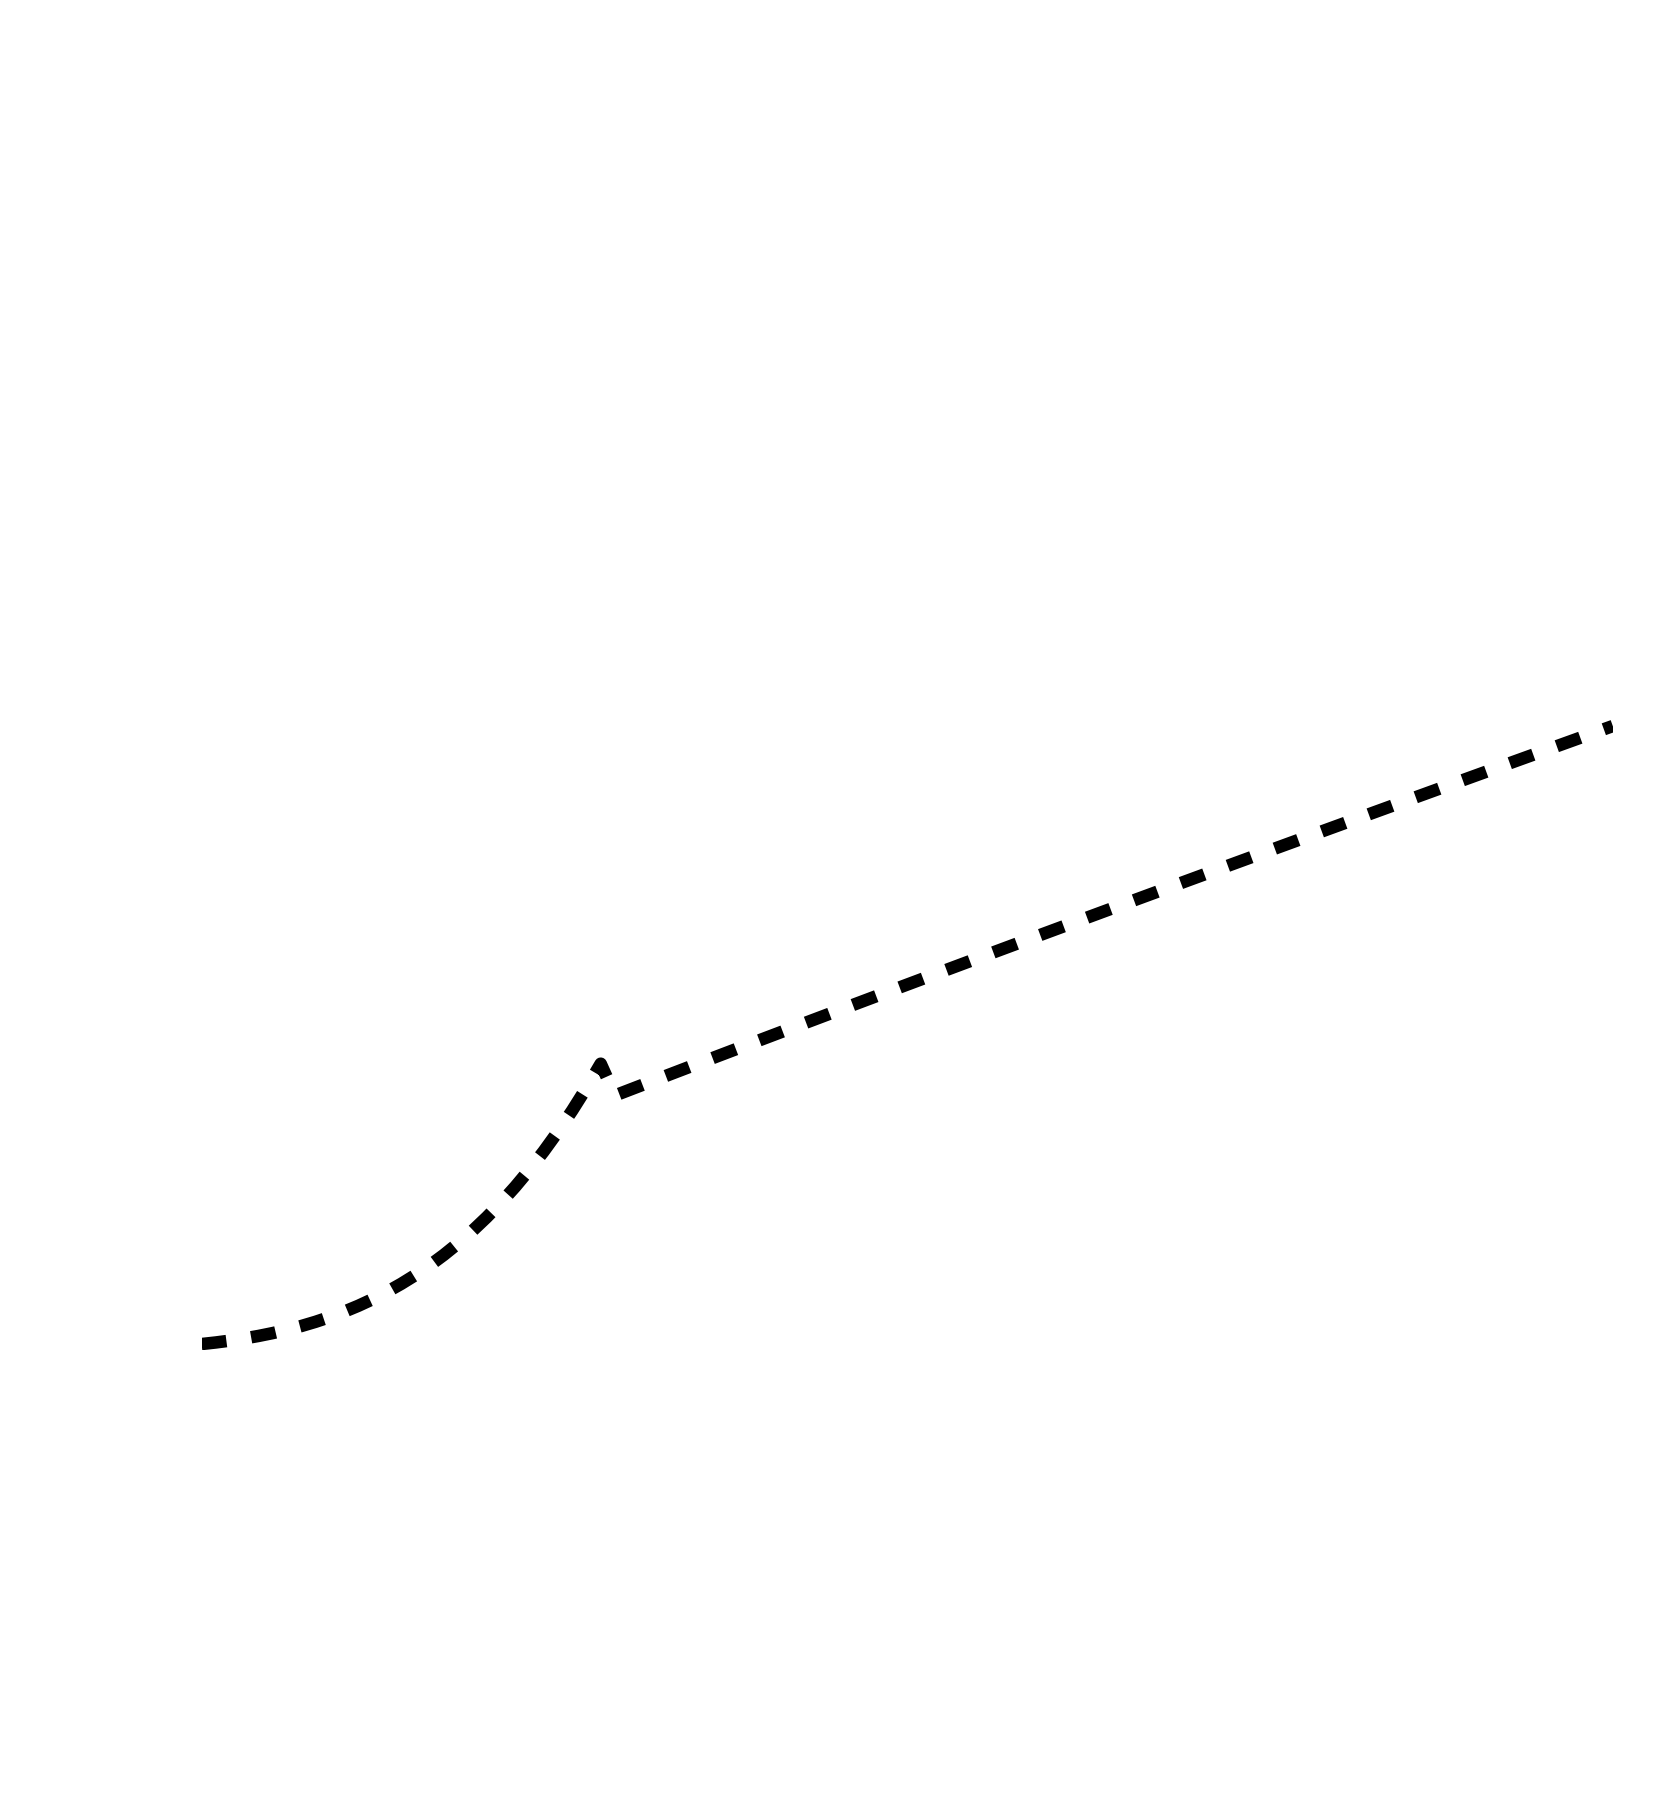
\includegraphics[width=0.6\hsize]{figures/MRscatter_curves.png}%
  \end{ocg}
  \hspace{-0.6\hsize}%
  \begin{ocg}{fig:eboff}{fig:eboff}{0}%
  \end{ocg}%
  \begin{ocg}{fig:ebon}{fig:ebon}{1}%
    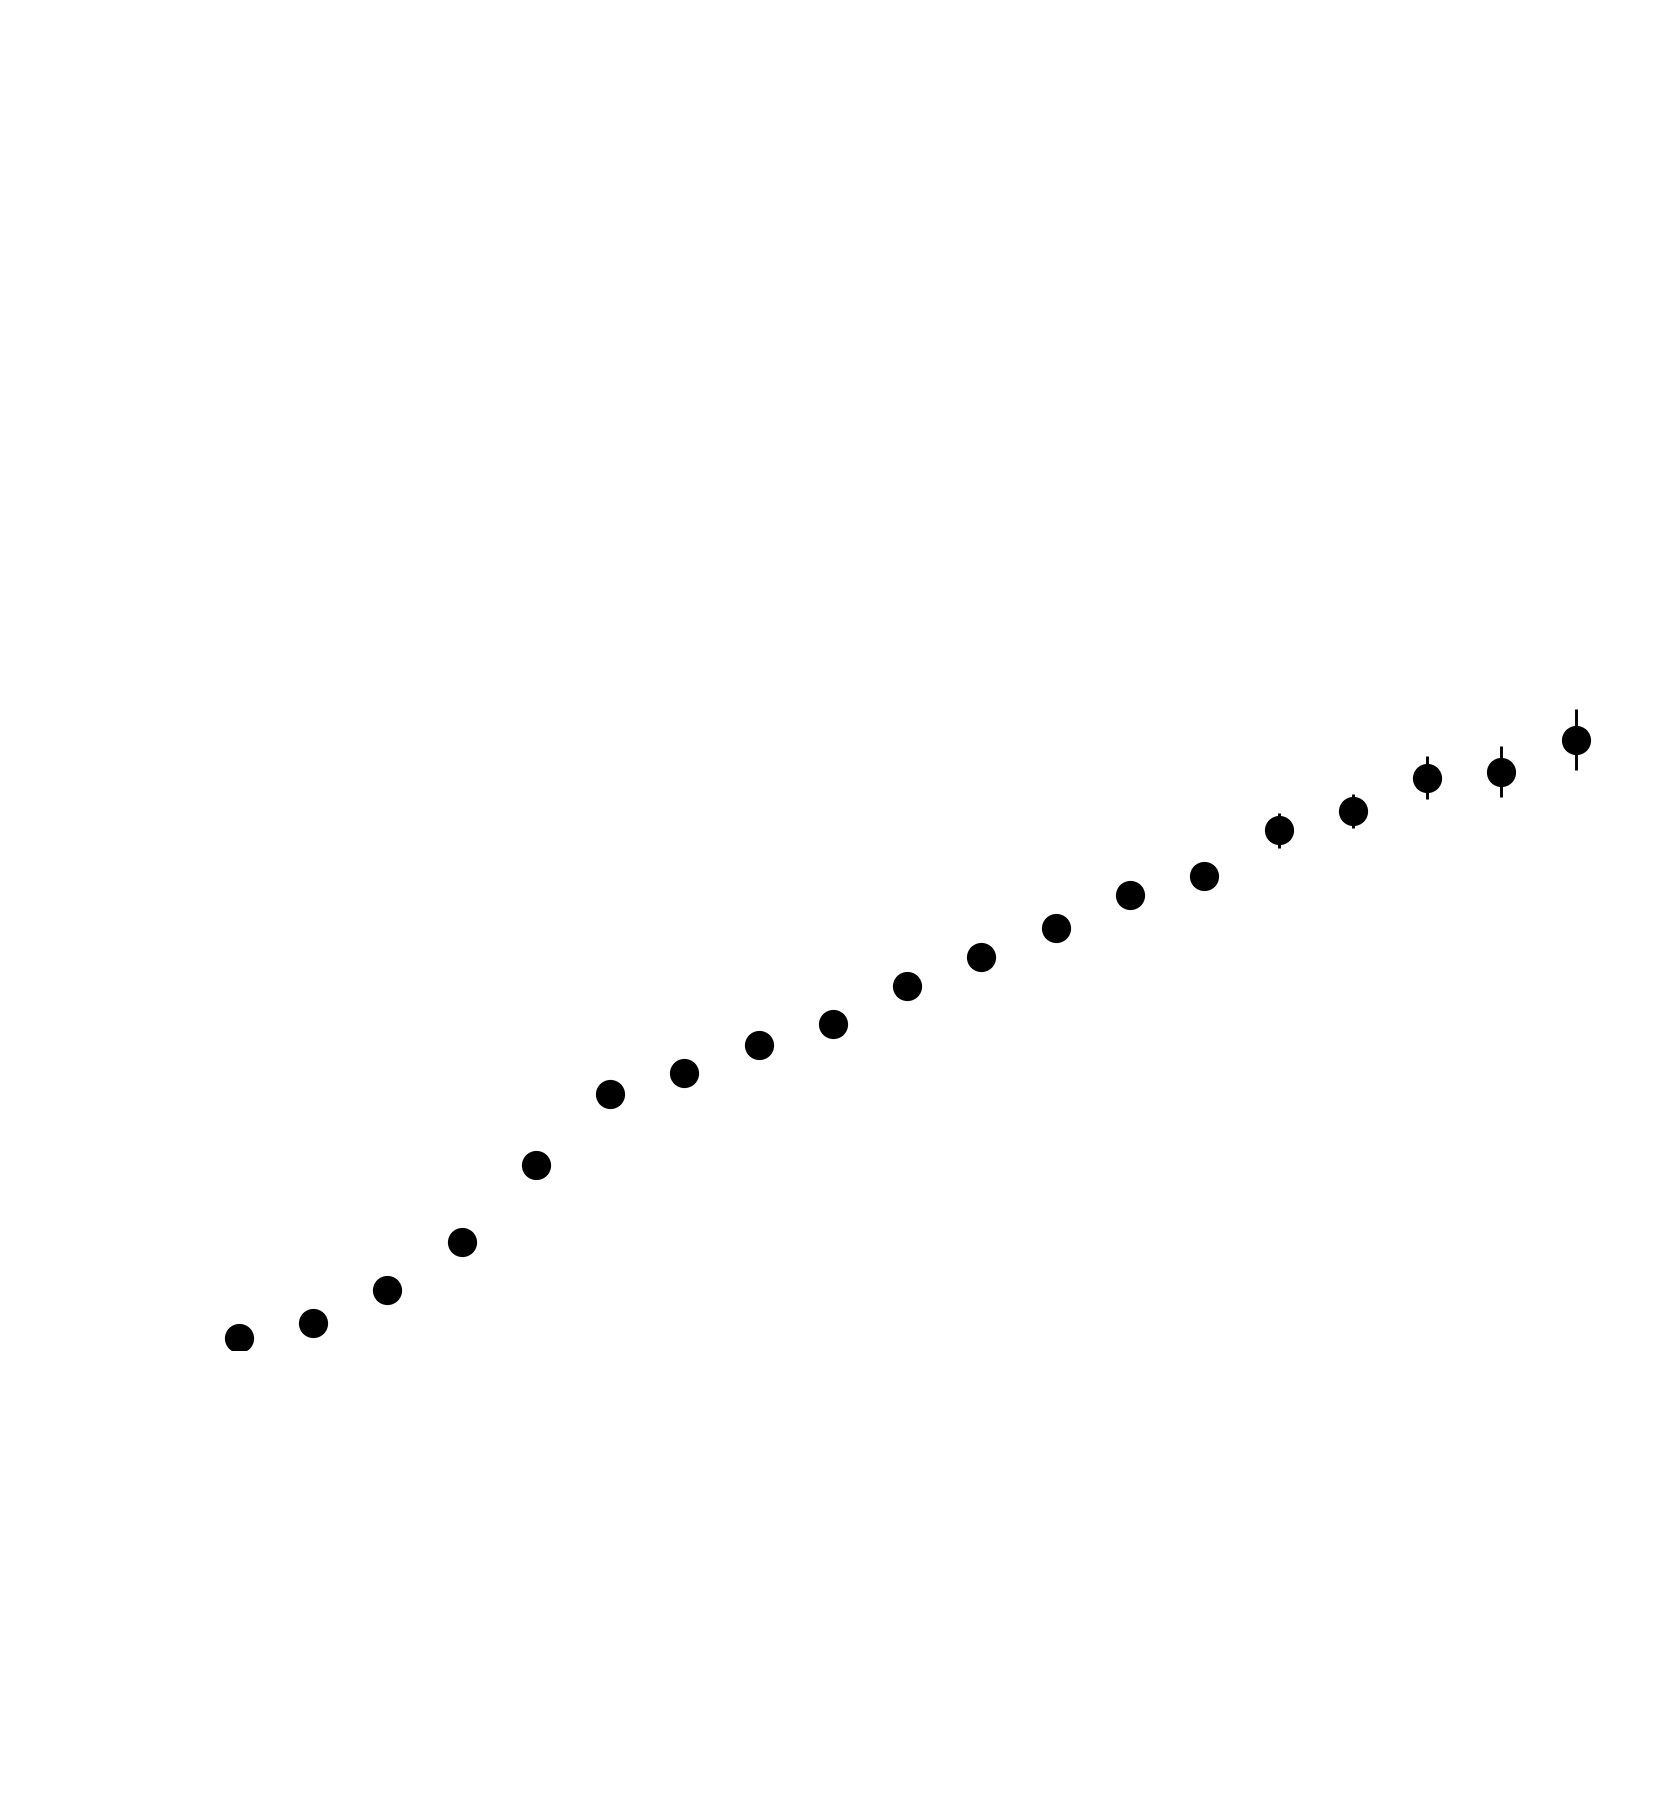
\includegraphics[width=0.6\hsize]{figures/MRscatter_scatter.png}%
  \end{ocg}
  \hspace{-0.6\hsize}%
  \caption[Masses and radii of synthetic planets in the simulated SLS-PS.]
    {\small 2D histogram depicting the masses and radii of the sampled
    small planet population with $r_p \leq 4$ R$_{\oplus}$. Planetary radii are drawn from the
    planet occurrence rates derived from Kepler and are mapped to 
    planetary masses using the mass-radius relation and Gaussian
    dispersion given in Eqs.~\ref{BSeq:mr} and \ref{BSeq:mrscat}. The mean
    mass-radius relation is over-plotted as the 
    \ToggleLayer{fig:curveon,fig:curveoff}{\protect\cdbox{\emph{dashed curves}}}. The mean
    planet mass and standard deviation of the mean in each planetary radius bin are plotted as
    \ToggleLayer{fig:ebon,fig:eboff}{\protect\cdbox{\emph{black circles}}} to
    show their close correspondence with the mean mass-radius relation.}
  \label{BSfig:mr}
\end{figure}

\emph{Restricted range of $P$ and $r_p$}. The second caveat with the Kepler-derived $f$ is that
we are restricted in
our range of sampled orbital periods and planetary radii as imposed by the size of the parameter space
for which $f$ is robustly measured with Kepler. Specifically, $f(P,r_p)$ from \cite{dressing15a}
is restricted to the orbital period domain of $P \in [0.5,200]$ days and the planetary radius domain of 
$r_p \in [0.5,4]$ R$_{\oplus}$ which includes small Mars-sized planets up to about the size of Neptune. 
However, given that the duration of the SLS-PS is longer than 200 days it is important to also consider planets
with orbital periods $> 200$ days. To inform the inclusion of such long period planets we use the RV M dwarf
survey detection of the non-zero frequency of giant planets 
(\msini{} $\ge 100$ M$_{\oplus}$) with orbital 
periods of $>200$ days albeit with a low $f$ \citep[$\lesssim 5$\%;][]{bonfils13}.
We therefore supplement the Kepler occurrence rates with draws 
from the HARPS occurrence rates of giant planets \citep{bonfils13}.
Long period planet sampling is carried out similarly to how the Kepler occurrence rates are sampled.
Here we draw the planetary minimum masses rather than planetary radii; $f \to f(P,m_p\sin{i})$.
We also note that in \cite{bonfils13} $f$ for giant planets is computed over a coarse grid
in minimum mass spanning an order-of-magnitude 
($10^2 \le m_p\sin{i}/\text{M}_{\oplus} \le 10^3$) despite the most massive HARPS detection having only
\msini{} $\sim 112$ M$_{\oplus}$. Therefore it is possible that giant planets with minimum masses in excess
of $\sim 112$ M$_{\oplus}$ ($0.3$ M$_{Jup}$) do not exist in nature around M dwarfs.
We note that throughout this study we will
primarily focus on the population of small planets from the Kepler-derived $f(P,r_p)$ 
because of their much larger frequency compared to giant planets around M dwarfs. \\

\emph{Applicability of occurrence rates to the full input catalog}.
Robust statistics regarding $f$ were derived from the 
sample of small Kepler stars which almost exclusively contained early-to-mid M dwarfs and late K-dwarfs.
The assumption that the resulting $f$ extend to later spectral
types is still largely uncertain but the early discovery of seven transiting Earth-sized planets around the
ultracool dwarf TRAPPIST-1 \citep{gillon17}, from a small sample of observed stars, hints that small planets
around late M dwarfs might be as common, and potentially more common than around the early M dwarfs observed
with Kepler. Preliminary estimates of $f$ around
late M dwarfs with \emph{K2} suggests a potential lack of super-Earth-sized planets on close-in orbits but have
been insufficient to probe the population of Earth-sized planets \citep{demory16}. Theoretically,
planet formation scenarios have also predicted the existence of many such small planets on close-in orbits
around late M dwarfs \citep[e.g.][]{alibert13,alibert17}. In Sect.~\ref{BSsect:2occ} we will investigate the
effect of increasing $f$ on our planet detections in the SLS-PS. \\

\emph{Dynamical considerations of multi-planet systems}.
The final caveat arises from $f(P,r_p)$ being derived in uncorrelated bins whereas dynamical constraints 
will prevent certain types of planetary systems from existing in nature. For example, close pairs
of massive planets. To ensure that sampled multi-planetary systems in our simulations are dynamically stable
we impose two priors on each system with multiplicity $> 1$.
The first constraint is the analytic assessment of Lagrange
stability \citep{barnes06} which only depends on the masses of the central star and planets, the planets'
semi-major axes, and eccentricities. For adjacent planet pairs that are Lagrange stable, by definition
their ordering remains fixed, both planets remain bound to the central star, and the criterion limits 
permissible changes in planets’ semi-major axes. Lagrange stability can be thought of as a more stringent
extension of Hill stability \citep{gladman93}. However we
note that the analytic treatment of Lagrange stability is only applicable to the three-body system.
In planetary systems from our simulations with $>2$ planets, we apply the Lagrange stability criterion
to every adjacent planet pair. We then supplement the Lagrange stability
criterion with the heuristic criterion from \cite{fabrycky12} which is applicable to systems with multiplicity
$>2$. The resulting criterion for stability\footnote{Long-term stability requires that
  $a_{\text{out}} - a_{\text{in}} \gtrsim 3.5$ $R_{\text{Hill}}$ where $a_{\text{in}}$ and $a_{\text{out}}$ are the
  semi-major axes of the inner and outer planet respectively and $R_{\text{Hill}}$ is their mutual Hill radius.}
is derived from the stability analysis of a set of numerical integrations. In our MC simulations
we only include multi-planetary systems which satisfy both aforementioned stability criteria. \\

As mentioned previously,
our dynamical considerations cause the injected planet population to not exactly match the adopted Kepler
occurrence rates. The modified Kepler planet occurrence
rates, or equivalently our injected planetary population, is shown in Fig.~\ref{BSfig:occurrence} as a function
of the input variables $P$ and $r_p$. We then report the same population after converting the planetary radii to
masses using Eqs.~\ref{BSeq:mr} and~\ref{BSeq:mrscat}. \\

\begin{figure}
  \centering
  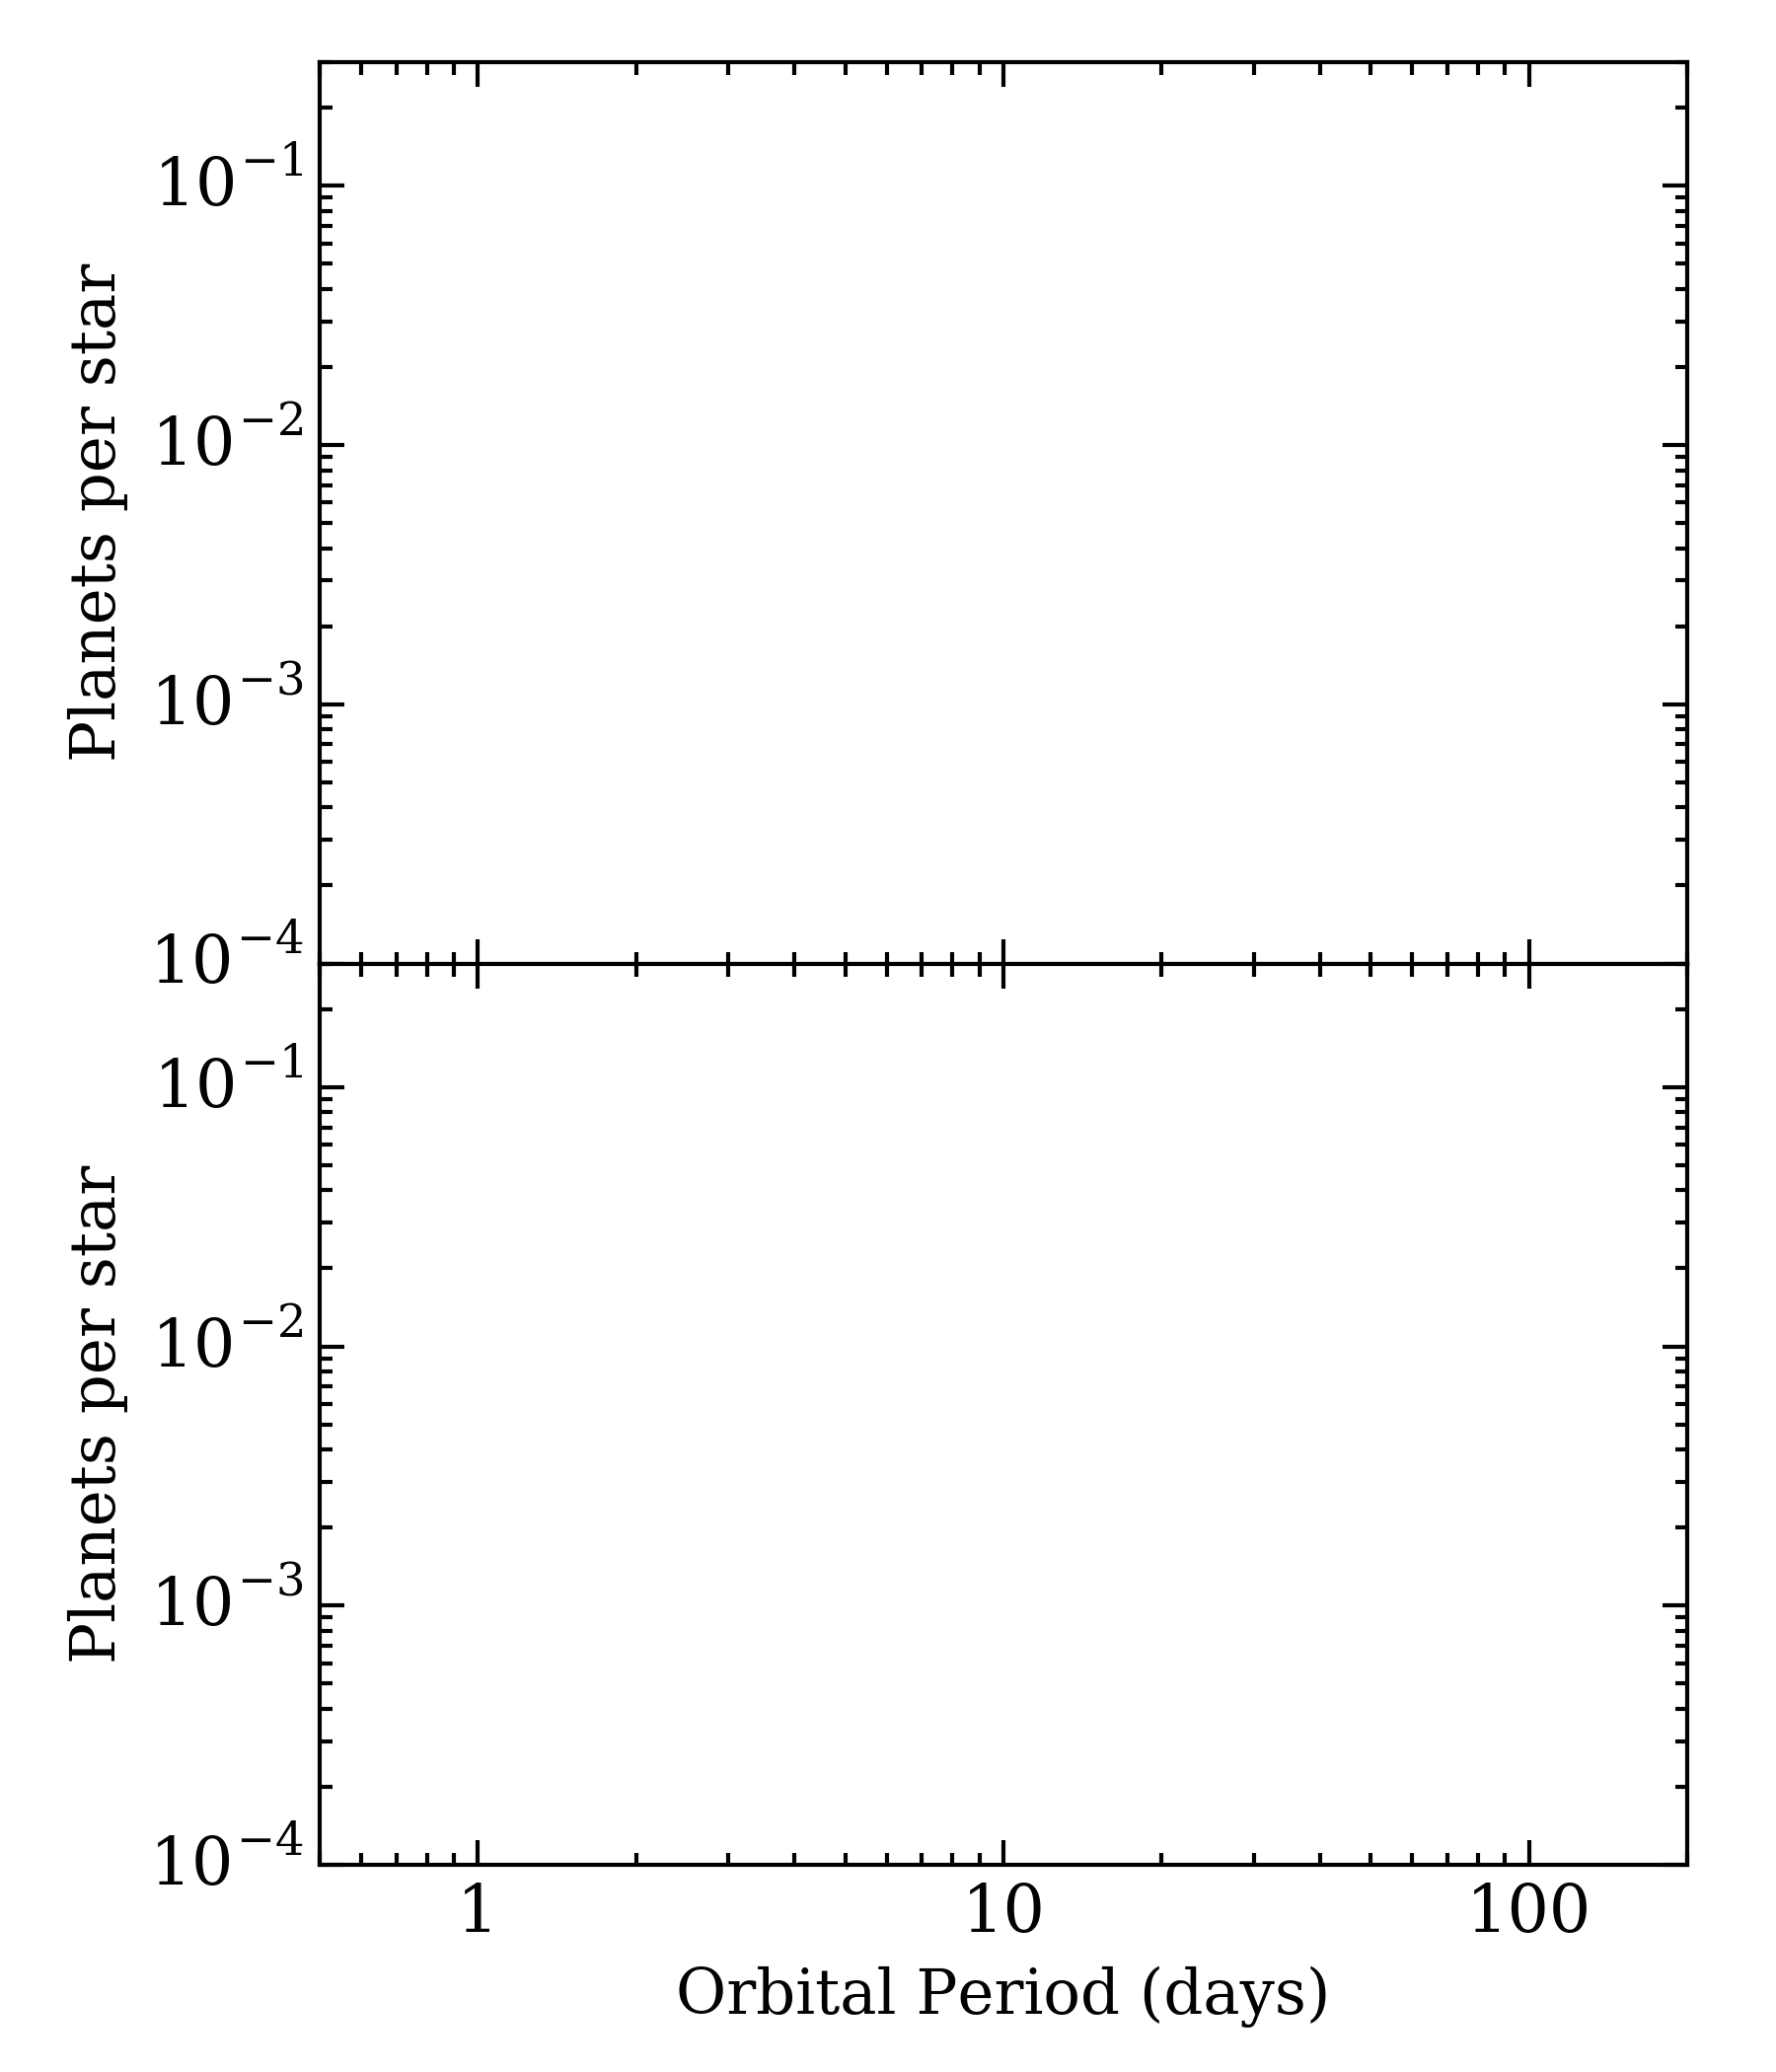
\includegraphics[width=0.8\hsize]{figures/mpoccurrence_bkgd.png}%
  \hspace{-0.8\hsize}%
  \begin{ocg}{fig:0off}{fig:0off}{0}%
  \end{ocg}%
  \begin{ocg}{fig:0on}{fig:0on}{1}%
    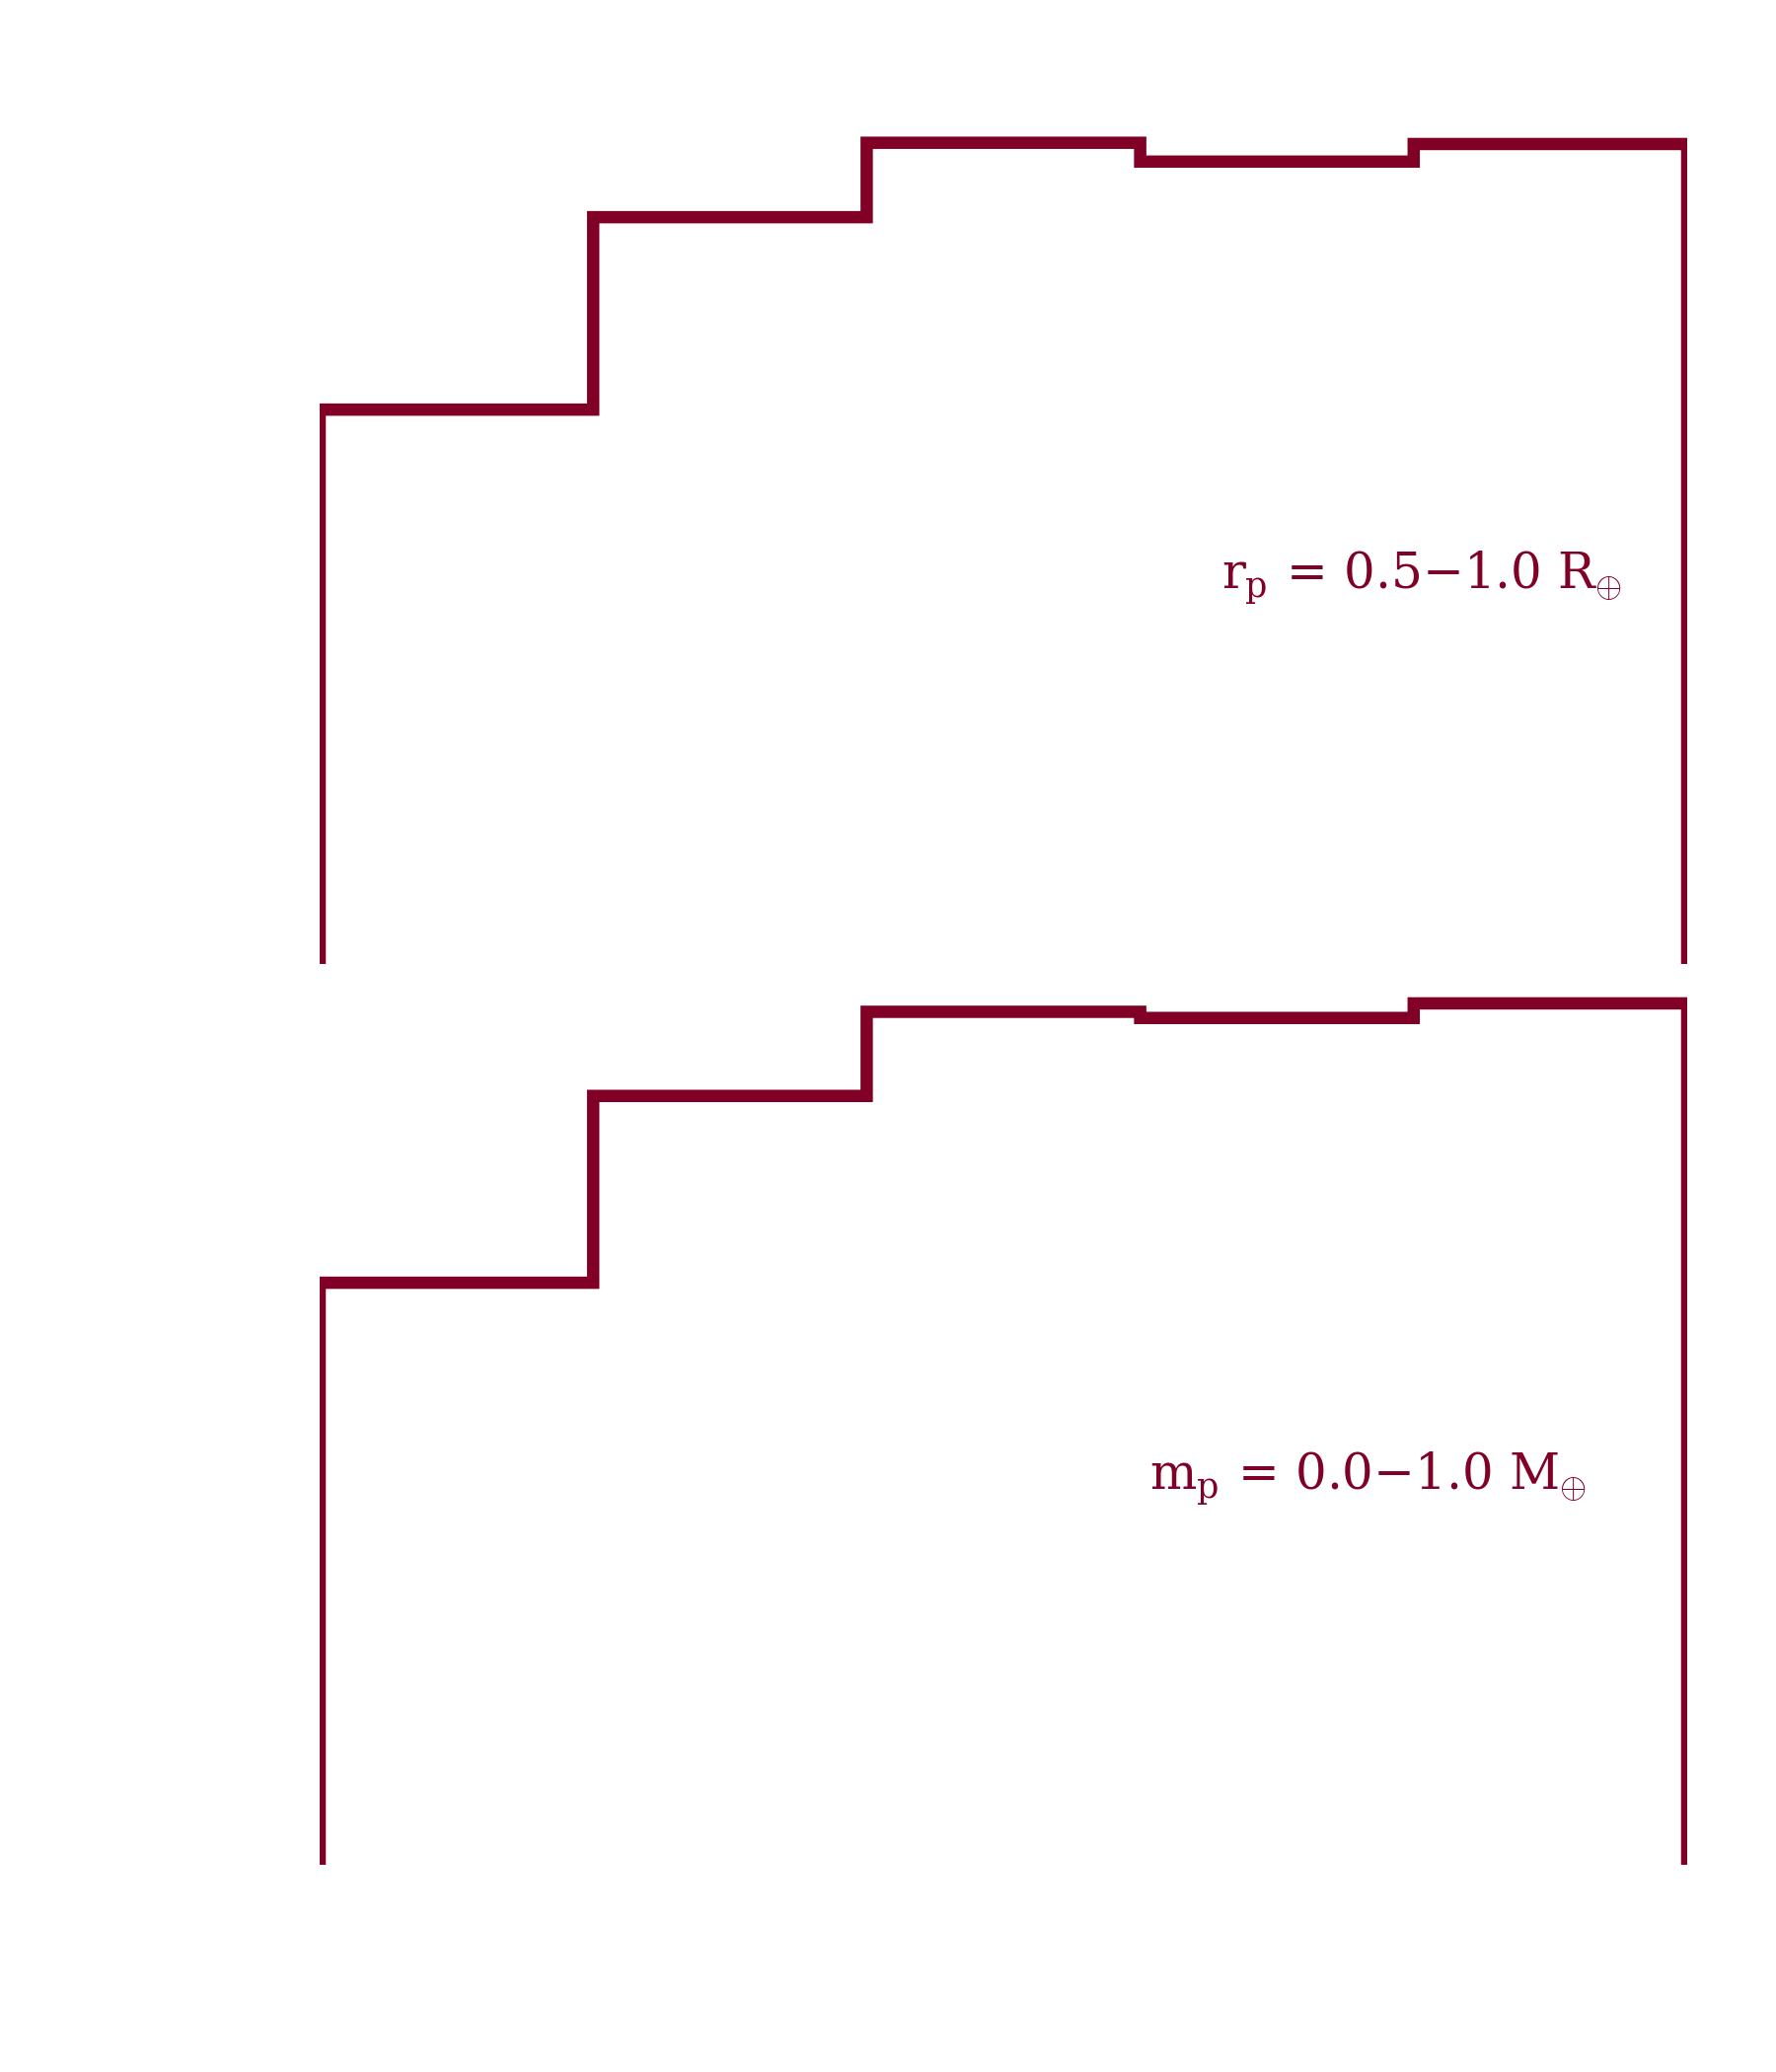
\includegraphics[width=0.8\hsize]{figures/mpoccurrence_0.png}%
  \end{ocg}
  \hspace{-0.8\hsize}%
  \begin{ocg}{fig:1off}{fig:1off}{0}%
  \end{ocg}%
  \begin{ocg}{fig:1on}{fig:1on}{1}%
    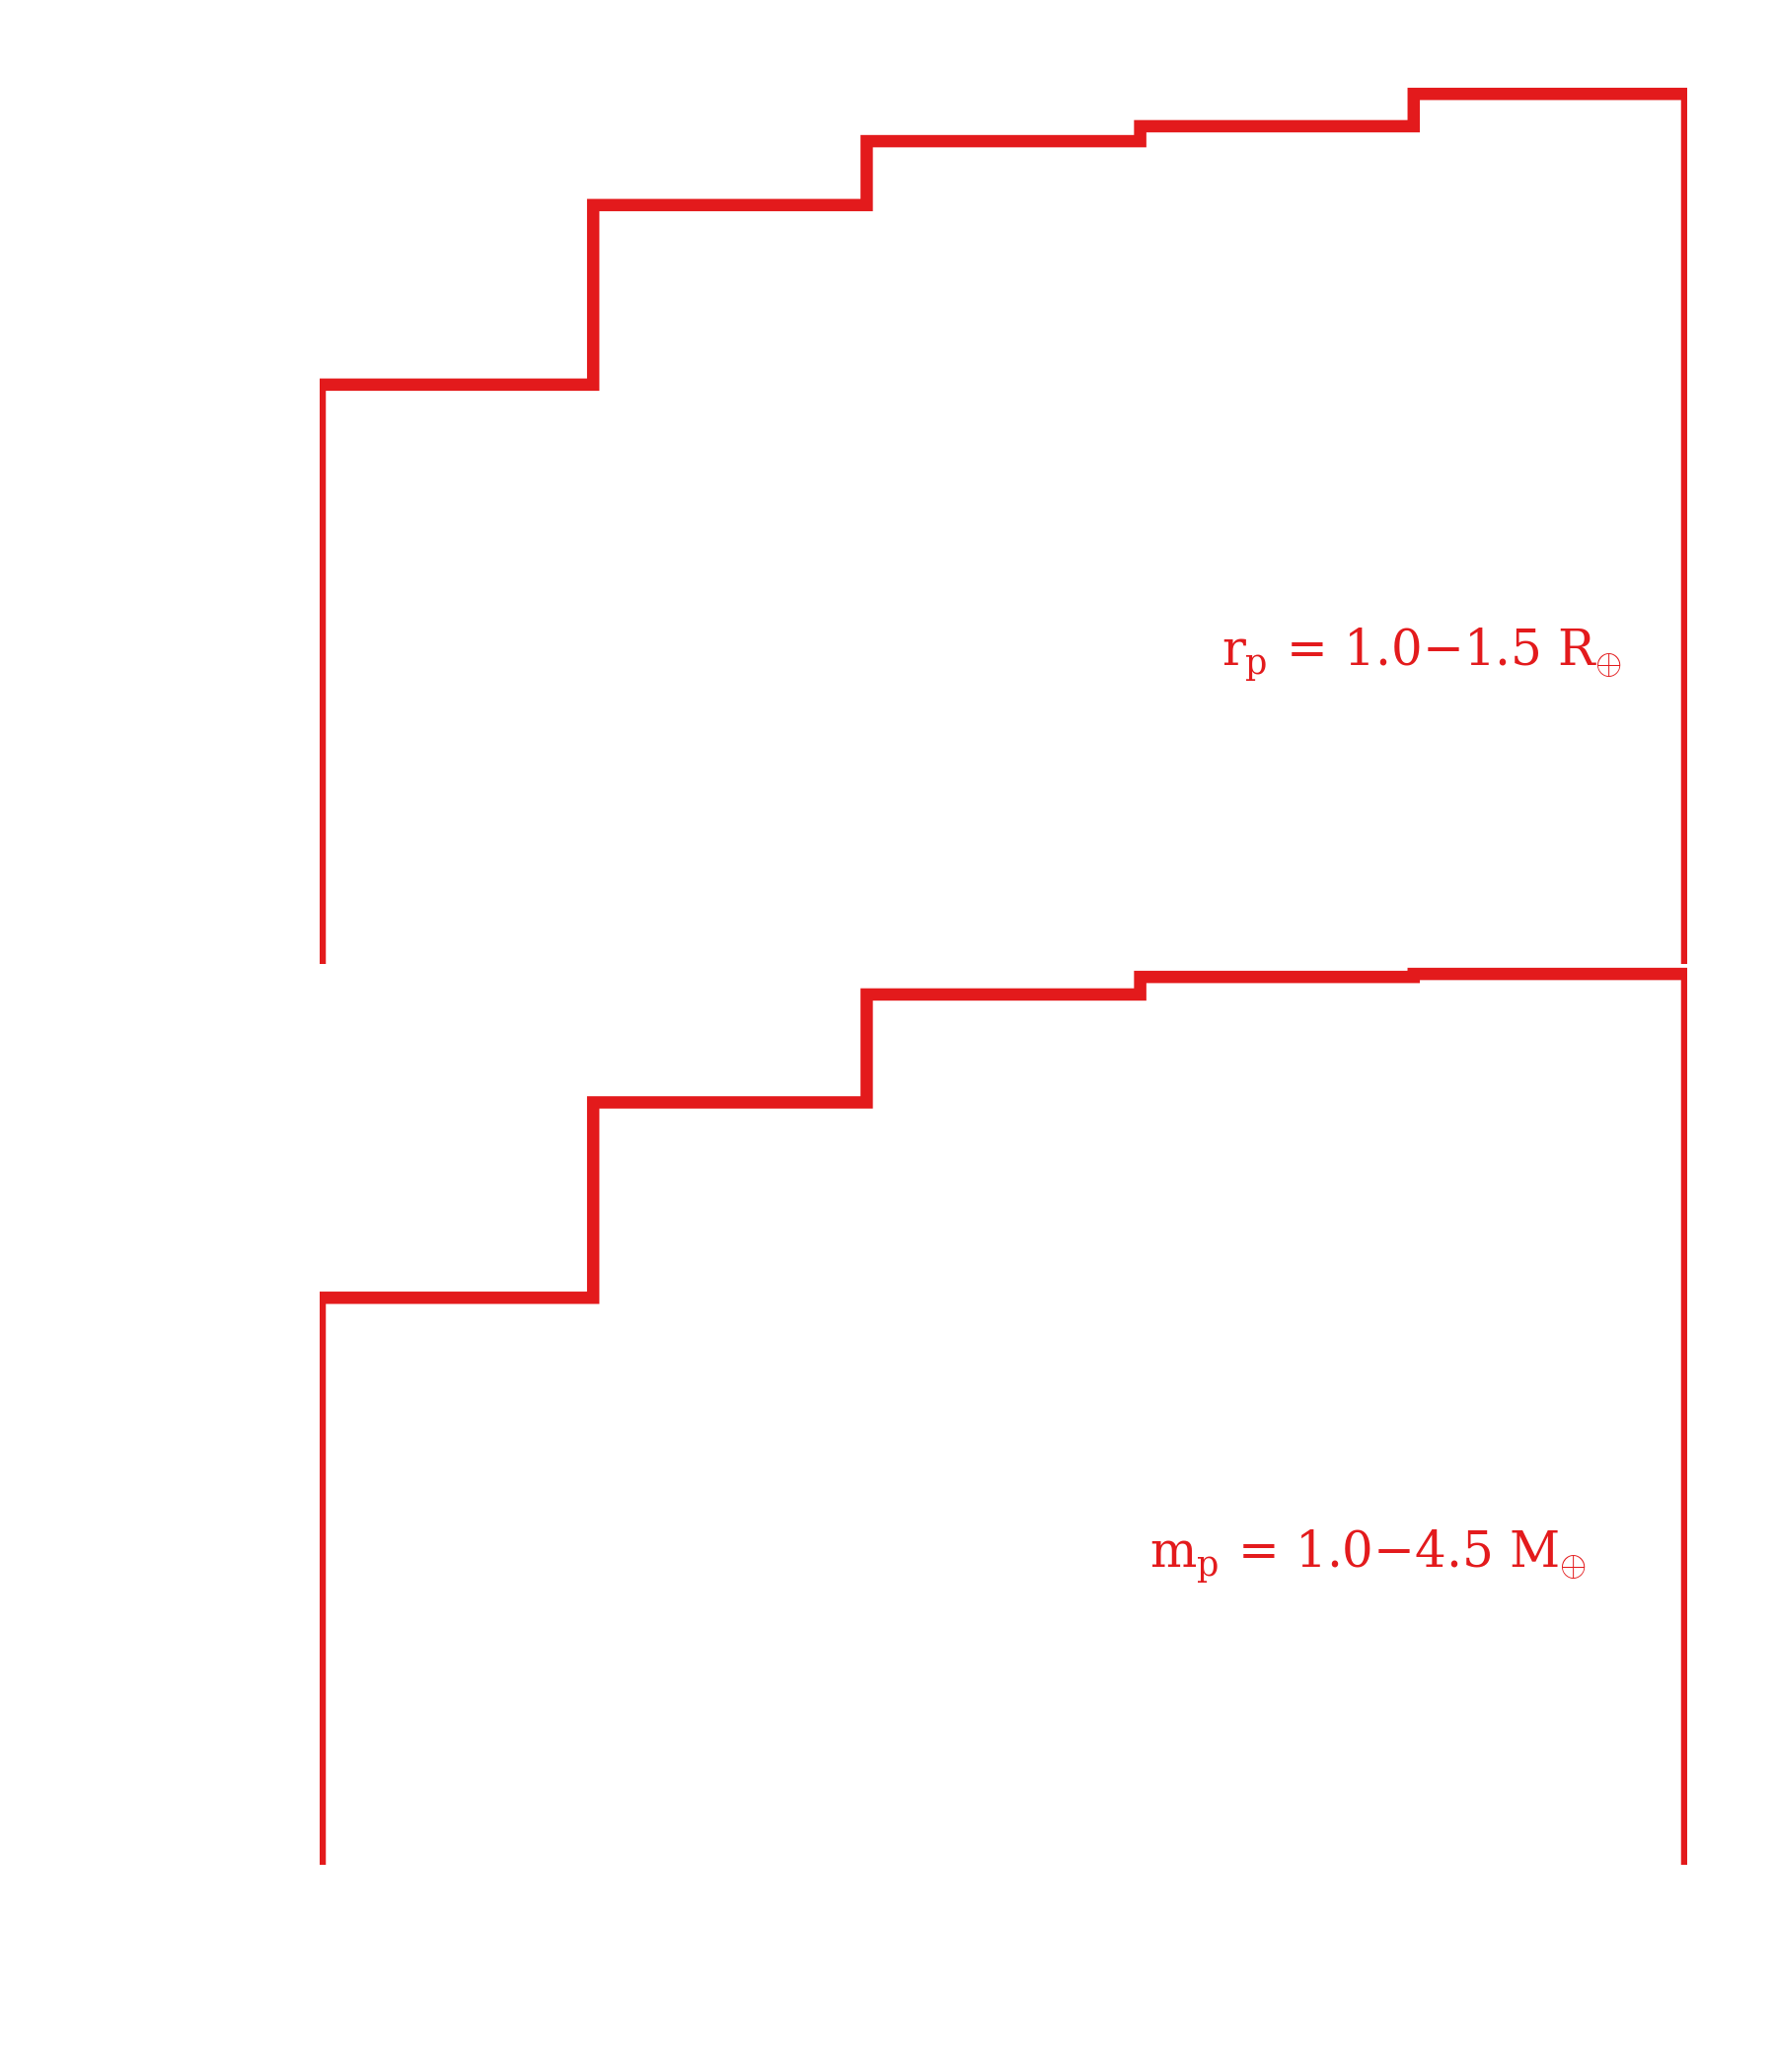
\includegraphics[width=0.8\hsize]{figures/mpoccurrence_1.png}%
  \end{ocg}
  \hspace{-0.8\hsize}%
  \begin{ocg}{fig:2off}{fig:2off}{0}%
  \end{ocg}%
  \begin{ocg}{fig:2on}{fig:2on}{1}%
    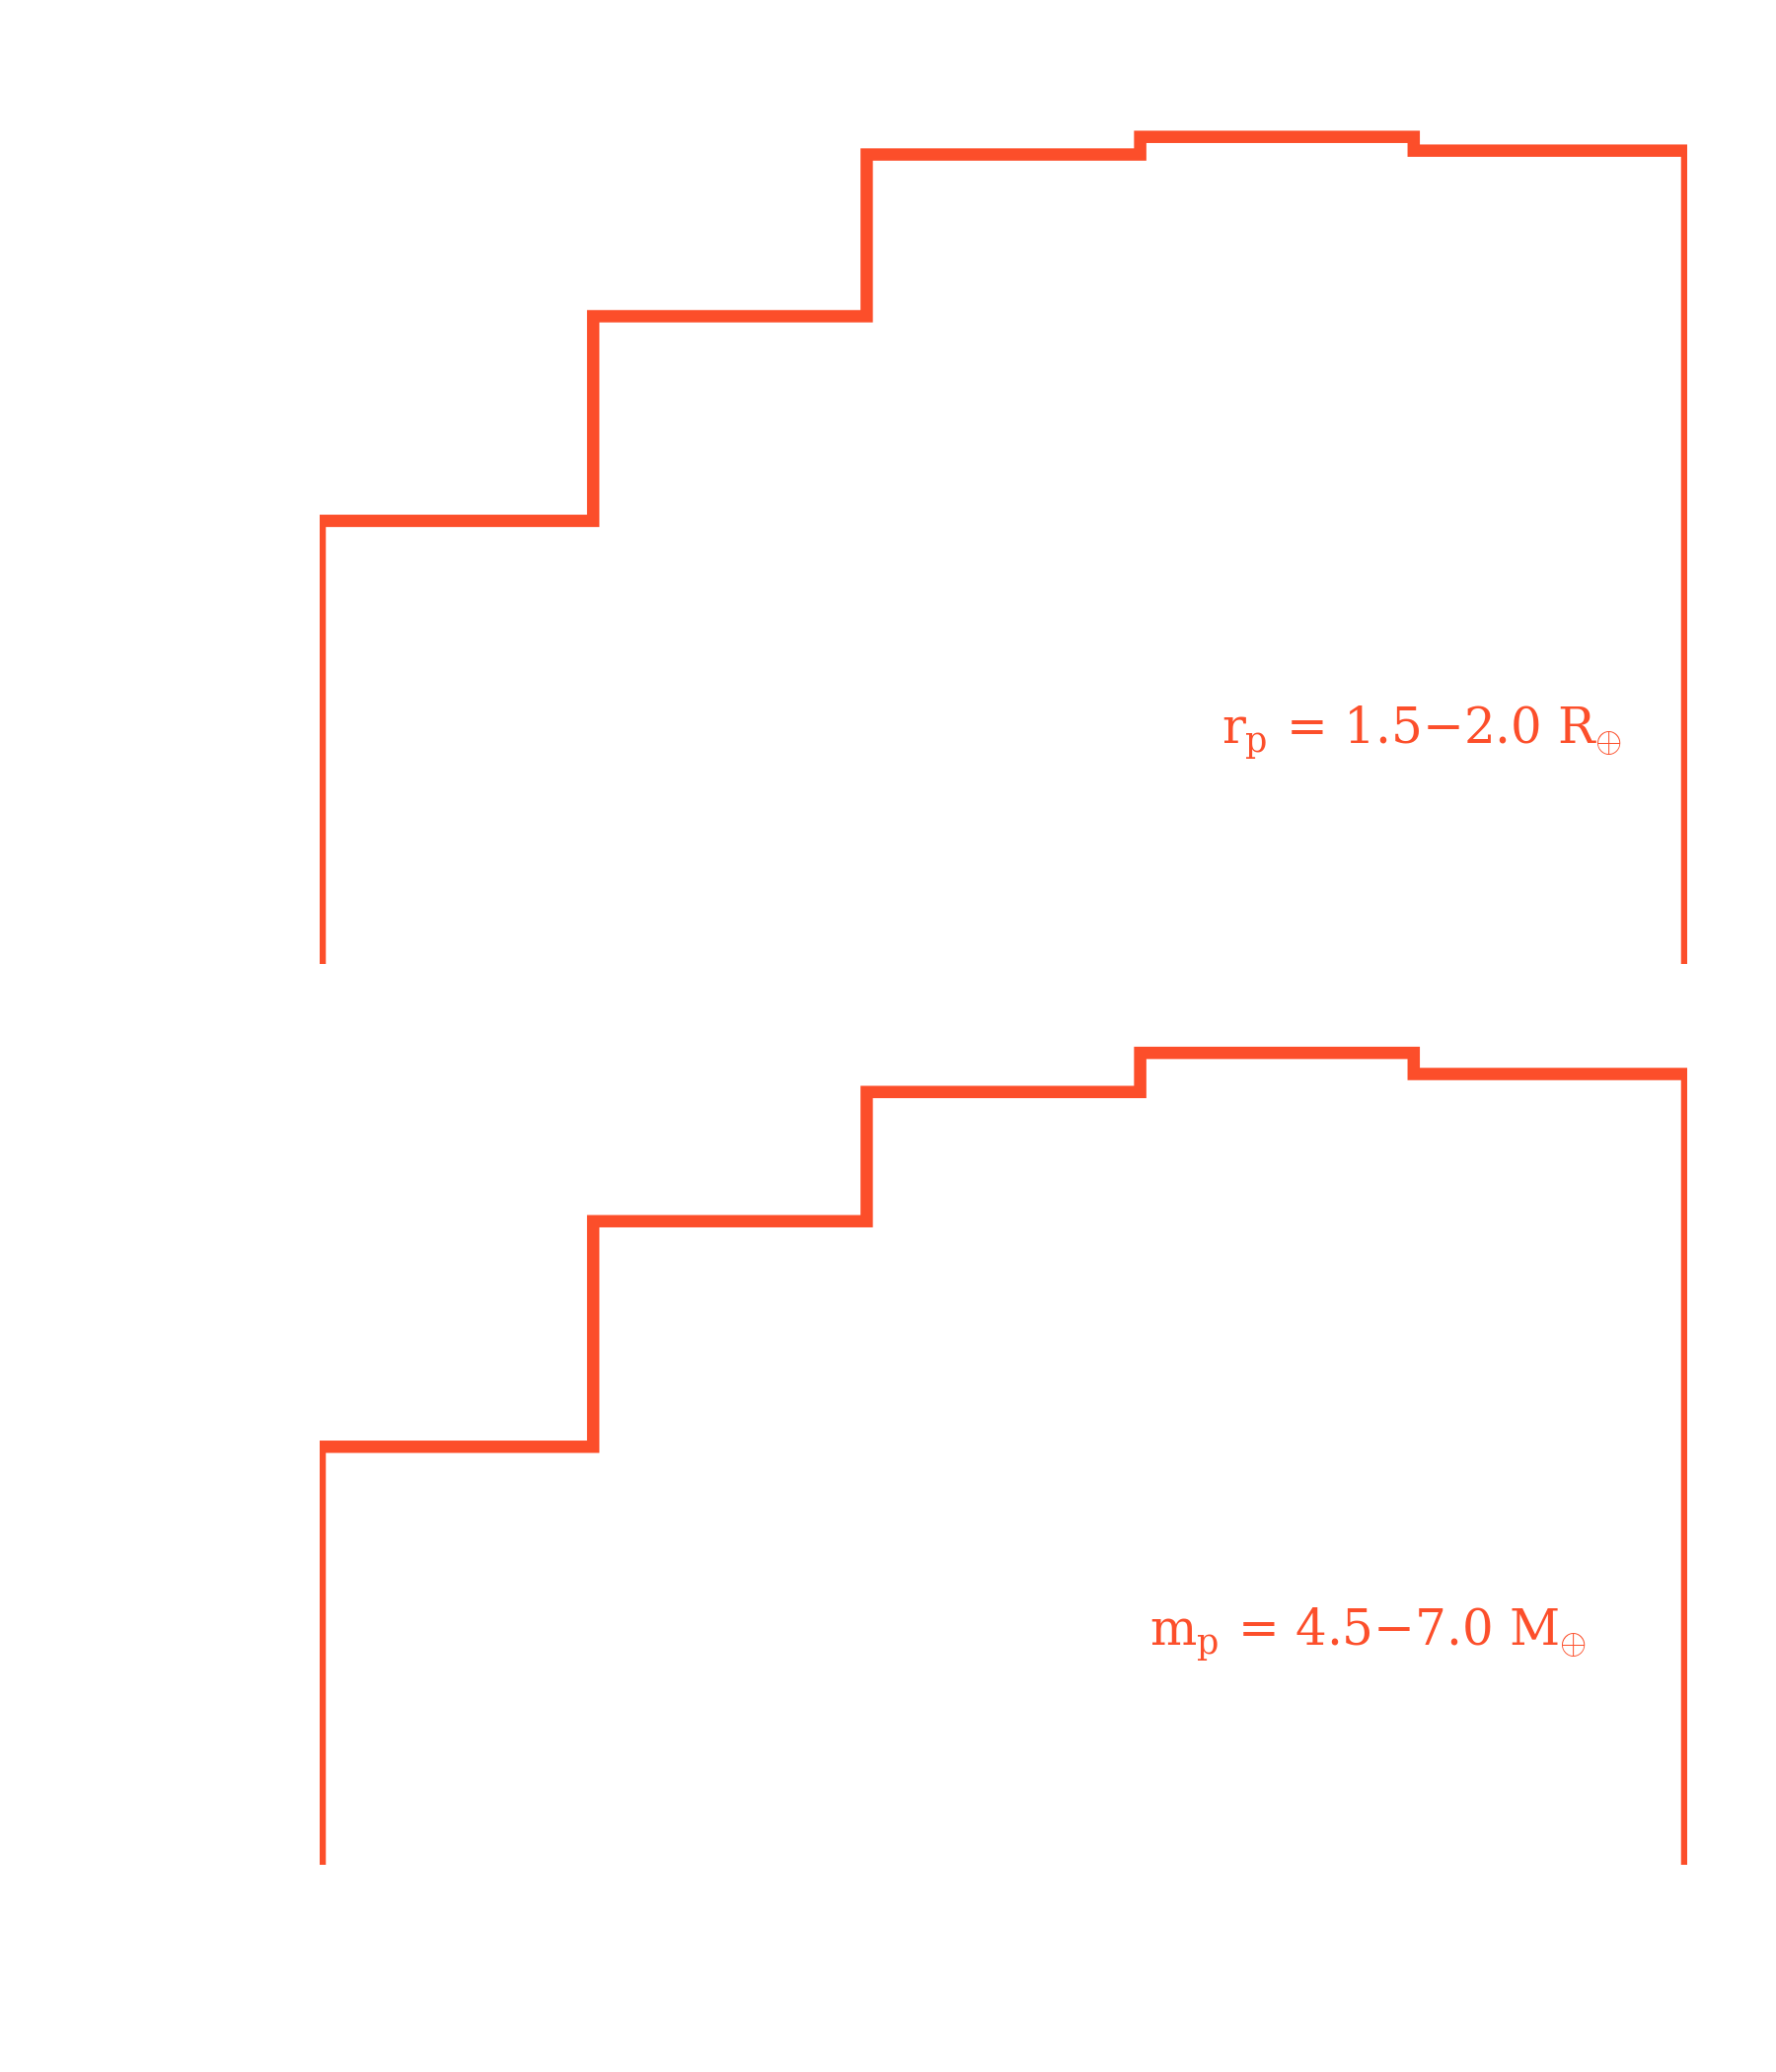
\includegraphics[width=0.8\hsize]{figures/mpoccurrence_2.png}%
  \end{ocg}
  \hspace{-0.8\hsize}%
    \begin{ocg}{fig:3off}{fig:3off}{0}%
  \end{ocg}%
  \begin{ocg}{fig:3on}{fig:3on}{1}%
    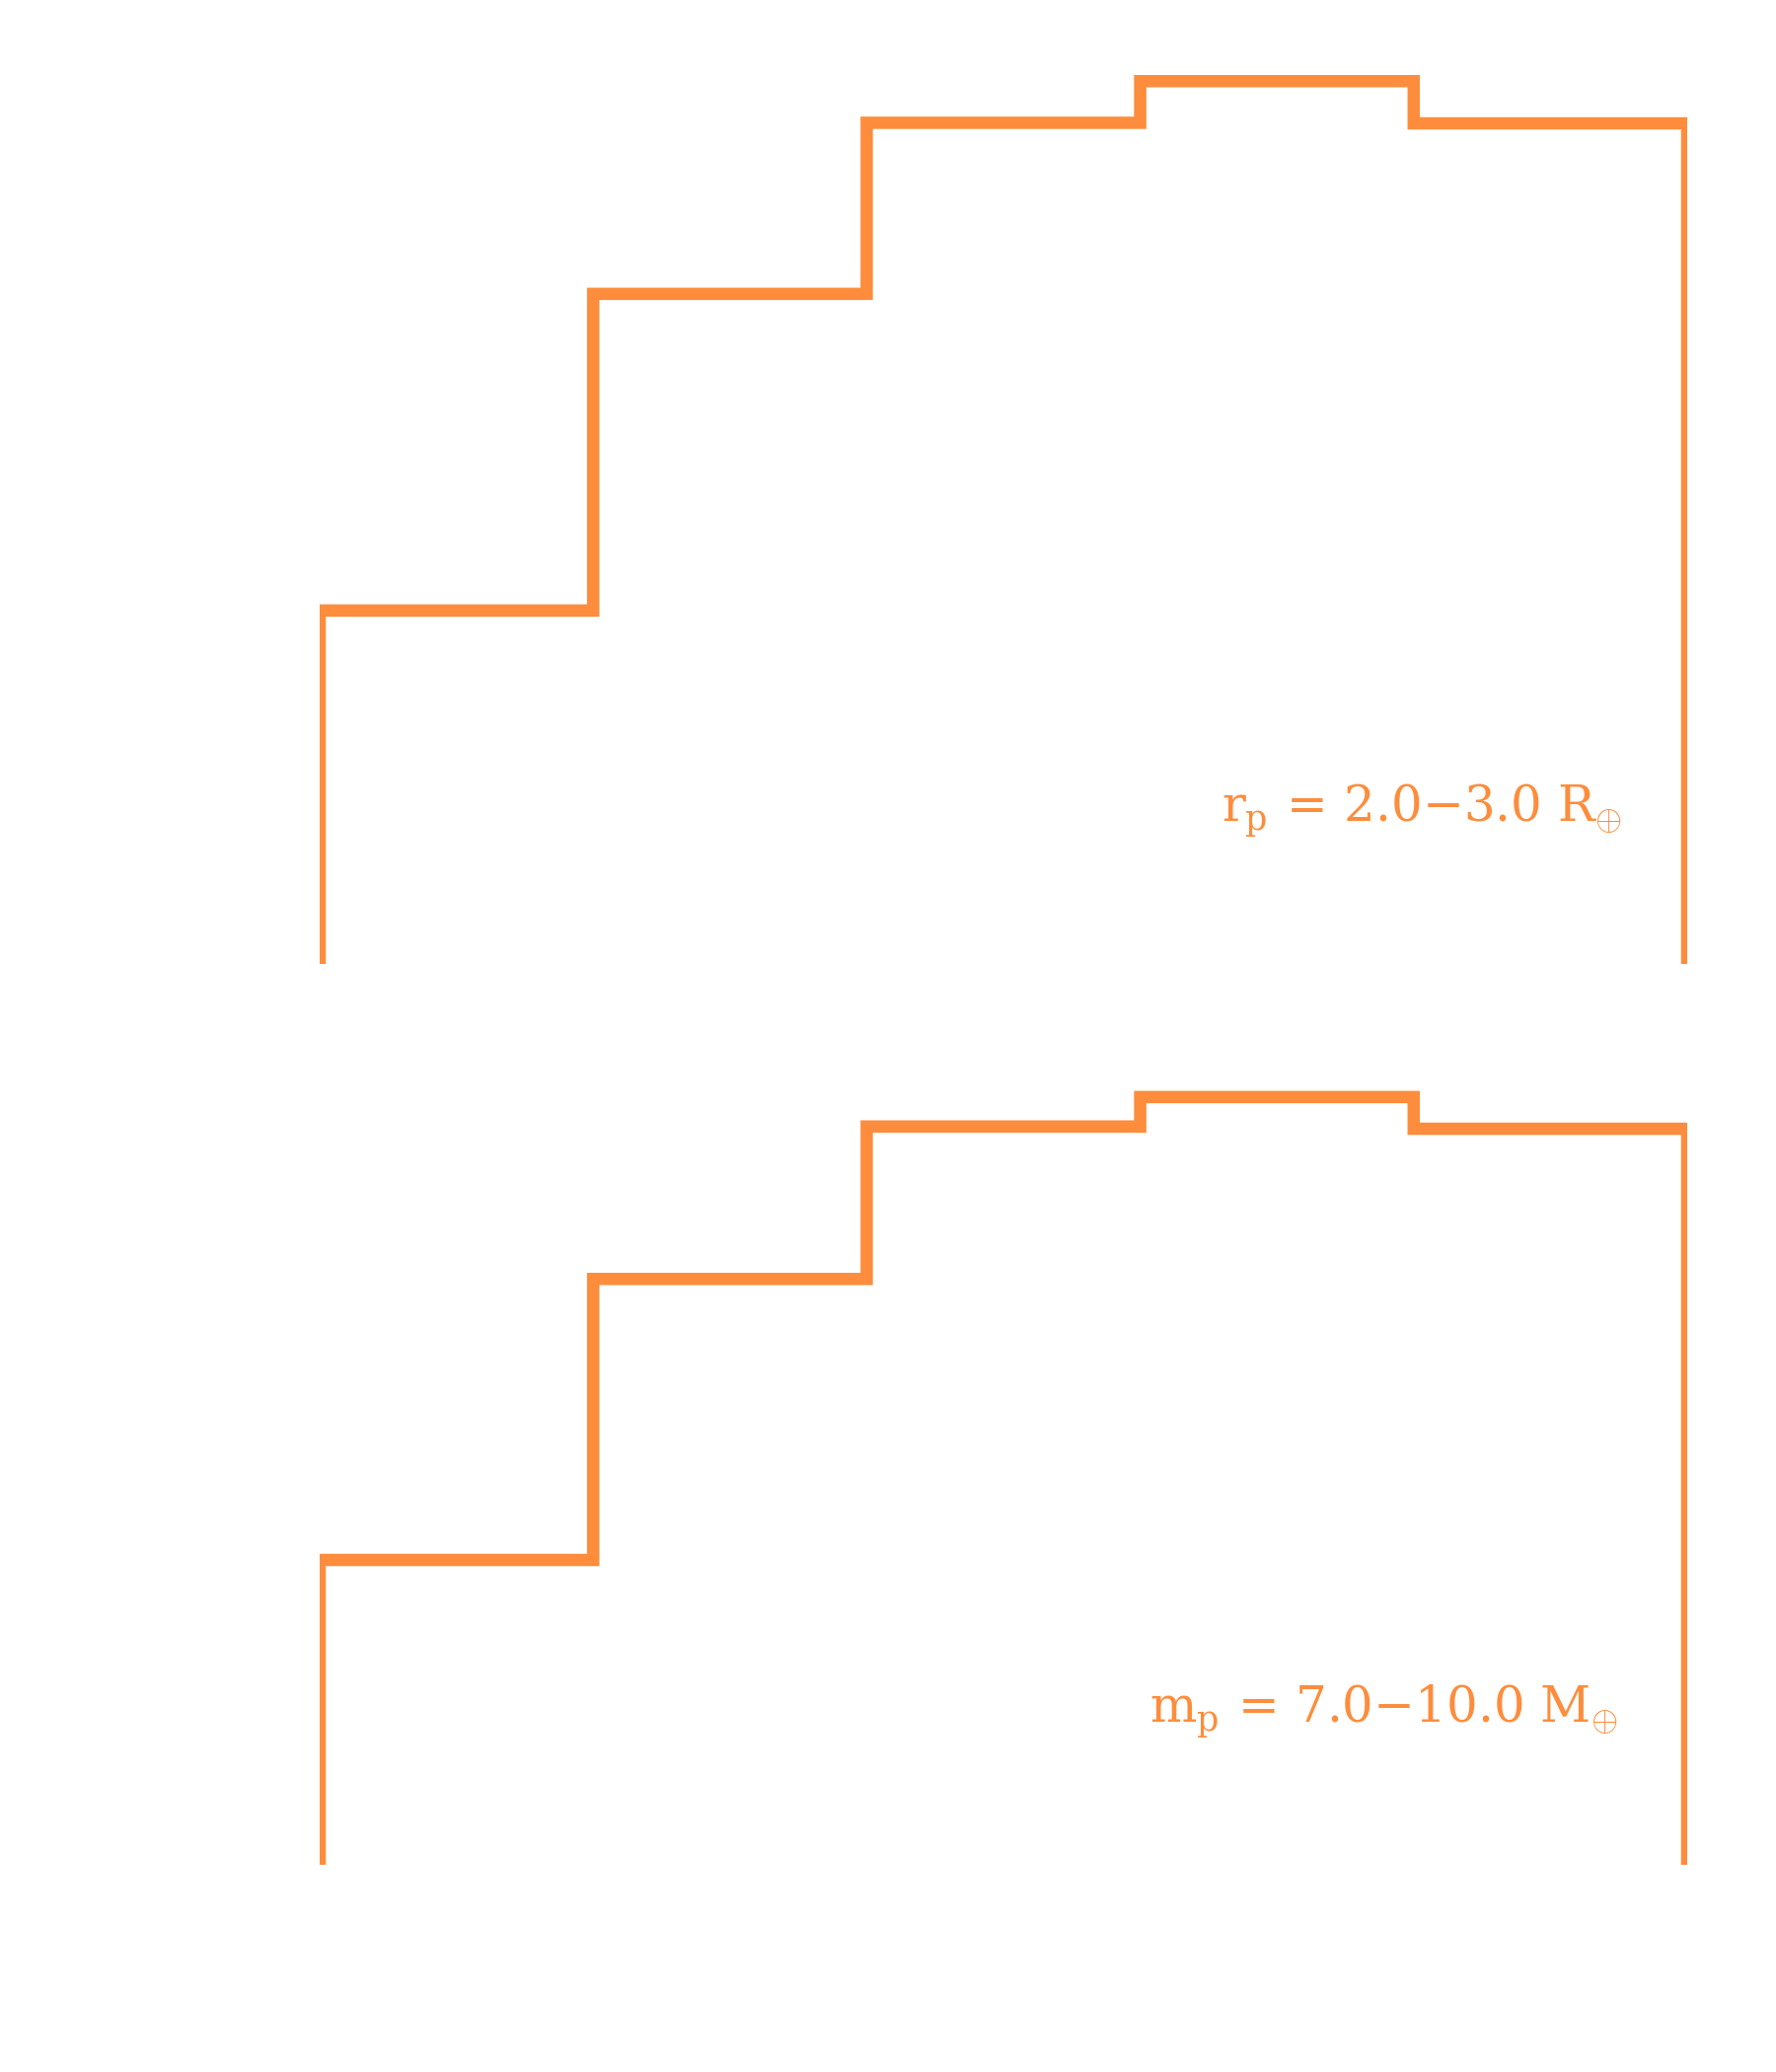
\includegraphics[width=0.8\hsize]{figures/mpoccurrence_3.png}%
  \end{ocg}
  \hspace{-0.8\hsize}%
    \begin{ocg}{fig:4off}{fig:4off}{0}%
  \end{ocg}%
  \begin{ocg}{fig:4on}{fig:4on}{1}%
    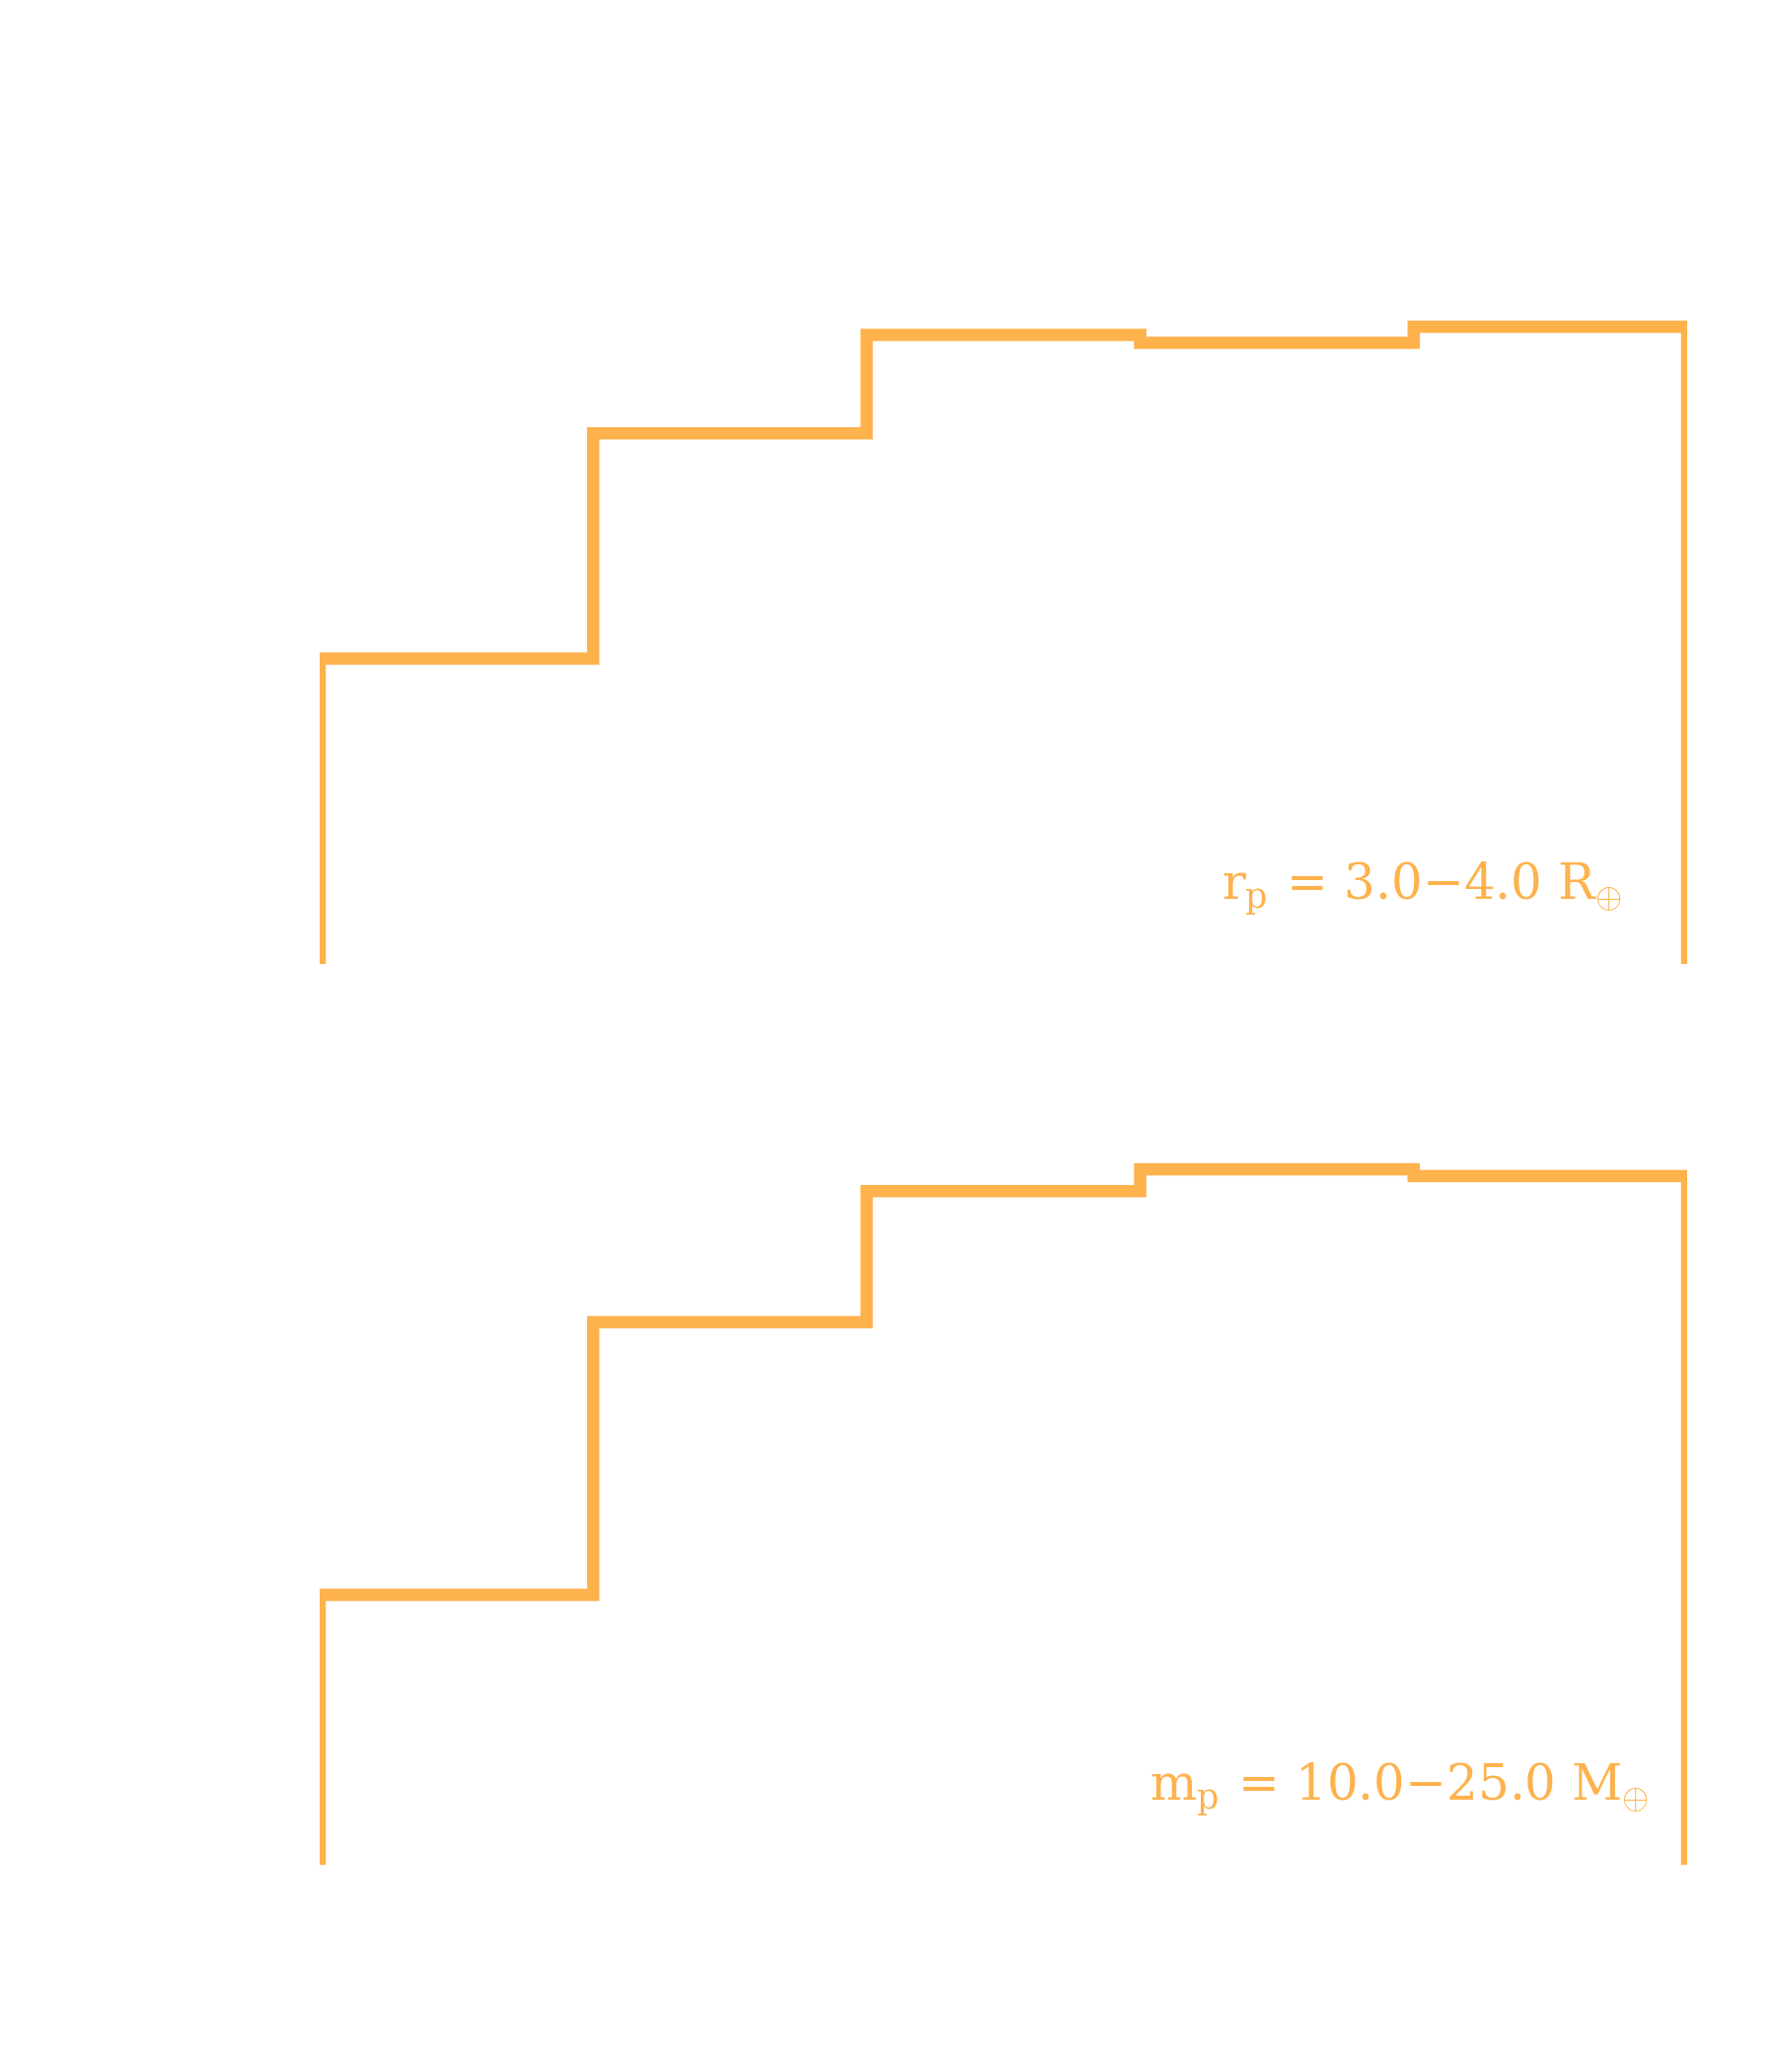
\includegraphics[width=0.8\hsize]{figures/mpoccurrence_4.png}%
  \end{ocg}
  \hspace{-0.8\hsize}%
  \caption[Input planet occurrence rates in the simulated SLS-PS.]
          {\small \emph{Top}: histograms of the injected small planet population in the simulated SLS-PS
    as a function of orbital period and planetary radius from \cite{dressing15a}. \emph{Bottom}:
    the same planet population as above converted to planetary mass using Eqs.~\ref{BSeq:mr}
    and~\ref{BSeq:mrscat}. For clarity each $r_p$ bin, and the approximately corresponding
    $m_p$ bin, can be viewed individually:
    \ToggleLayer{fig:0on,fig:0off}{\protect\cdbox{$r_{p,min}=0.5$ R$_{\oplus}$}},
    \ToggleLayer{fig:1on,fig:1off}{\protect\cdbox{$r_{p,min}=1$ R$_{\oplus}$}},
    \ToggleLayer{fig:2on,fig:2off}{\protect\cdbox{$r_{p,min}=1.5$ R$_{\oplus}$}},
    \ToggleLayer{fig:3on,fig:3off}{\protect\cdbox{$r_{p,min}=2$ R$_{\oplus}$}},
    \ToggleLayer{fig:4on,fig:4off}{\protect\cdbox{$r_{p,min}=3$ R$_{\oplus}$}}.}
  \label{BSfig:occurrence}
\end{figure}

The resulting distribution of planetary system multiplicities is shown in Fig.~\ref{BSfig:mult}.
Simulated planetary systems that obey our dynamical stability criteria contain 0-7 planets although only 0.04\%
of simulated planetary systems can survive with 7 planets. Similarly, $\sim 4$\% of simulated planetary systems contain
no planets at all. 
The most common planet multiplicity is 2 with $\sim 32$\% of simulated planetary systems containing 2 planets. The resulting
average planet multiplicity is $\sim 2.4$ which is slightly less than the cumulative injected multiplicity of
$2.5 \pm 0.2$. When
recovering the planet yield of our simulated survey we will have to correct for this small discrepancy between the
cumulative planet multiplicity of our injected population and the \emph{true} multiplicity of 2.5 for planets
with $P \in [0.5,200]$ days and $r_p \in [0.5,4]$ R$_{\oplus}$ (see Sect.~\ref{BSsect:yield}).

\begin{figure}
  \centering
  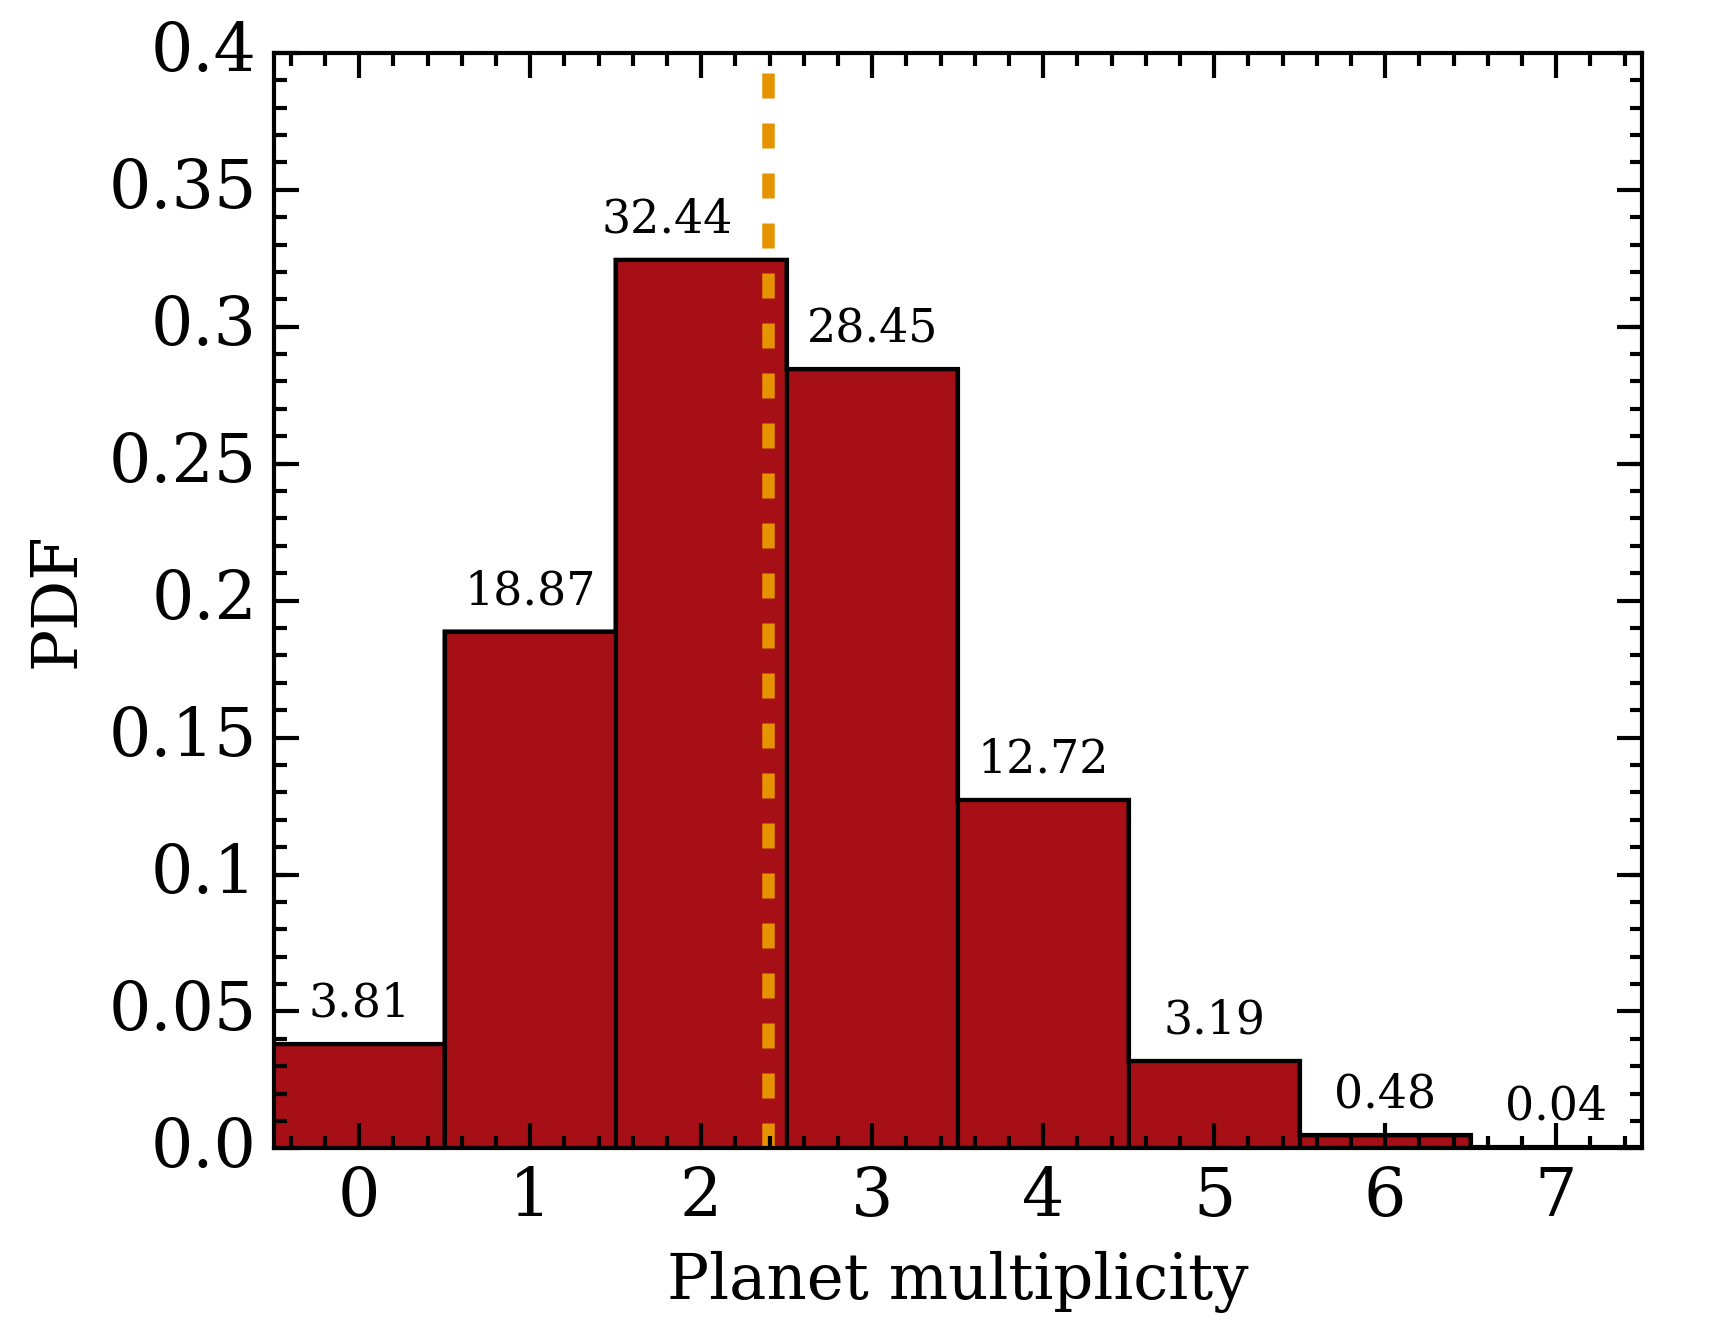
\includegraphics[width=0.6\hsize]{figures/multhist.png}%
  \caption[Histogram of planetary system multiplicities in the simulated SLS-PS.]
      {\small The probability density function of planet multiplicities in the simulated SLS-PS.
    The fraction of simulated systems with a given multiplicity---in percentage---is annotated for
    each integer multiplicity. We find an average planet multiplicity of $\sim 2.4$ which is highlighted by the
    \emph{vertical dashed line} and is slightly less than the cumulative injected multiplicity of 2.5 planets
    with $P\leq 200$ days from \cite{dressing15a}.}
  \label{BSfig:mult}
\end{figure}


\section{Activity Mitigation} \label{BSsect:GP}
\subsection{Overview of the Gaussian Process Formalism}
RV activity signals present in M dwarfs (e.g. Gl176, \citealt{forveille09}; Gl674, \citealt{bonfils07},
Proxima Centauri; \citealt{robertson16}) will deter our ability to detect new exoplanets in the SLS-PS.
A number of correction techniques have been developed by various groups
within the field to mitigate these effects and detect planets in RV \citep[see reviews in][]{fischer16, dumusque17}.
One particularly promising method is the use of Gaussian process regression to model correlated noise (i.e. activity)
in RV time-series. \\

Gaussian processes (GP) belong to a class of \emph{non-parametric} regression models from the field of machine-learning
\citep{rasmussen05}.
Being non-parametric, the functional form of the activity model is unspecified and instead is determined by the
data itself. In this way the GP activity model does not assume 
any physical model of the underlying processes responsible for the observed activity. Instead the GP is
used to model the covariance properties 
of an input time-series according to a user-defined covariance function which itself is described by a small number
of hyperparameters\footnote{`Small' compared to the size of the input time-series which would be required to fully
  describe the covariance properties of the input dataset.}.
%Because of this, GP regression models are sometimes referred to as
%\emph{semi-parametric}.
By its non-parametric nature, GP regression is an attractive method for modelling the stochastic processes that give
rise to observable stellar activity. \\

The GP prior distribution, which is described by the aforementioned covariance function,
is a multi-variate Gaussian distribution of functions specified by a mean function
$\boldsymbol{\mu}(\mathbf{t})$, evaluated at the epochs contained in the window function $\mathbf{t}$,
and a covariance matrix

\begin{equation}
  K_{ij} = \sigma_i^2 \delta_{ij} + k(t_i,t_j). \label{BSeq:K}
\end{equation}

\noindent which
is computed from the vector of measurement uncertainties $\boldsymbol{\sigma}(\mathbf{t})$,
the Kronecker delta function $\delta_{ij}$, and
the user-defined covariance function $k(t_i,t_j)$ describing the covariance between two measurements taken at
times $t_i$ and $t_j$for $i,j \in [1,n_{\text{obs}}]$.
Obtaining the GP model of an arbitrary input time-series $\mathbf{y}$ and uncertainty vector
$\boldsymbol{\sigma}$ is done by maximizing the Gaussian logarithmic likelihood function

\begin{equation}
  \ln{\mathcal{L}} = -\frac{1}{2} \left( (\mathbf{y}-\boldsymbol{\mu})^T K^{-1}
  (\mathbf{y}-\boldsymbol{\mu}) + \ln{\mathrm{det} K} + n_{\text{obs}} \ln{2 \pi} \right), \label{BSeq:like}
\end{equation}
  
\noindent to obtain the `best-fit' values of the GP hyperparameters describing the covariance of the observations
$\mathbf{y}$ through the covariance function $k(t_i,t_j)$.
In the case of M dwarfs, activity predominantly arises from rotationally modulated ARs which also
evolve in time due to their varying lifetimes, spatial distribution, and contrast.
Because of this temporal evolution we adopt a quasi-periodic covariance function
of the form

\begin{equation}
k(t_i,t_j) = a^2 \exp{\left[ - \frac{|t_i-t_j|^2}{2\lambda^2} -\Gamma^2
    \sin^2{\left(\frac{\pi|t_i-t_j|}{P_{\text{GP}}} \right)} \right]}, \label{cov}
\end{equation}

\noindent described by four hyperparameters: $a$ the amplitude of the covariance in the units of $\mathbf{y}$,
$\lambda$ the exponential decay of correlations, $\Gamma$ the coherence scale of correlations,
and $P_{\text{GP}}$ the periodic timescale. 
From identical reasoning to our own, quasi-periodic covariance functions are commonly adopted in a
number of related astrophysical applications such as the recovery of stellar rotation periods (i.e.
setting $P_{\text{GP}}=P_{\text{rot}}$) \citep[e.g.][]{angus18} and to the modelling of RV activity
from spectroscopic activity diagnostics \citep[e.g.][]{haywood14, rajpaul15, cloutier17b}, 
photometry \citep[e.g.][]{cloutier17a, cloutier17b}, or the raw RVs themselves
\citep[e.g.][]{faria16, donati17, yu17} and is applicable when the baseline of the
observations spans at least a few rotation periods \citep{pont13}. \\
 
Following the optimization of the GP hyperparameters one obtains a unique GP prior distribution. Conditioning
the GP prior on the dataset $\mathbf{y}(\mathbf{t})$ results in the GP predictive distribution whose mean function
and posterior variance can be evaluated at previously unseen epochs $\mathbf{t}^*$ via

\begin{equation}
  \boldsymbol{\mu}(\mathbf{t}^*) = K(\mathbf{t}^*,\mathbf{t}) \cdot K(\mathbf{t},\mathbf{t})^{-1} \cdot \mathbf{y}(\mathbf{t})
  \label{BSeq:GPmean}
\end{equation}

\noindent and 

\begin{equation}
  C(\mathbf{t}^*) = K(\mathbf{t}^*,\mathbf{t}^*) - K(\mathbf{t}^*,\mathbf{t}) \cdot K(\mathbf{t},\mathbf{t})^{-1} \cdot
  K(\mathbf{t}^*,\mathbf{t})^T.
  \label{BSeq:GPvar}
\end{equation}

\noindent Here the covariance matrix $K(\mathbf{t}^*,\mathbf{t}^*)$ is evaluated at unseen epochs such that
$\boldsymbol{\sigma}(\mathbf{t}^*)$ must be set to zero in Eq.~\ref{BSeq:K}.


\subsection{Modelling RV Activity with GP Regression} \label{BSsect:regression}
As in nature, the RV time-series from our MC simulations contain contributions from both planetary companions
as well as activity from ARs. These sources of the RV activity signals also have manifestations in other
spectroscopic time-series, albeit not strictly at the same rotation period \citep{hebrard16}. One example is the
full width at half maximum (FWHM) of the CCF which we simulate along with the RV signals (see Sect.~\ref{BSsect:activity}).
As is often the case when searching for small planets
in RV, one cannot distinguish a-priori an RV signal from a planet or from activity. However the covariance
properties in the FWHM time-series will be related to the covariance properties in RV residuals after the removal
of planetary sources. We therefore use the FWHM time-series to train the hyperparameters of our quasi-periodic
GP prior distribution. In principle one could have chosen an alternative activity indicator such as the BIS or
contrast of the CCF however recent HARPS observations have demonstrated that the strongest correlations between the RVs and
an activity indicator often exist between the RV and FWHM time-series 
(e.g. \citealt{astudillodefru17a}, Bonfils et al. 2017b in prep). However
this is not universal. Similarly, the contrast or depth of the CCF is not used in place
of the FWHM because although the two time-series are highly correlated, the CCF contrast is known to be more strongly
affected by instrumental noise in practice.
Using a spectroscopic training set like the FWHM also has the benefit of being obtained contemporaneously with the
RV measurements therefore probing the star's activity at the same epochs in which we are searching for planets.
In this way our GP activity model is also sensitive to variations in the RV activity occurring on long timescales such as
from magnetic activity cycles. \\

To reduce computational wall time of our full MC simulation
we do not compute a GP activity model in each MC realization of our simulated
SLS-PS. The GP activity model is only computed when the rms of the injected RV activity exceeds the median RV measurement
uncertainty. In such cases we run a Markov Chain Monte-Carlo
(MCMC) on the FWHM time-series to obtain the marginalized posterior probability density functions (PDF)
of the four GP hyperparameters: $a,\lambda,\Gamma$, and $P_{\text{GP}}$.
To sample the posterior PDFs we use the \texttt{emcee} affine invariant
MCMC ensemble sampler \citep{foremanmackey13} coupled with the fast GP package \texttt{george} 
\citep{ambikasaran15} to evaluate the likelihood function in Eq.~\ref{BSeq:like}.
Specifically we initialize 100 walkers with an effective chain length
$\sim 10$ autocorrelation times to ensure convergence of the chains.
Samples of the posterior PDFs are only saved following a burn-in phase of $\sim 10$ autocorrelation times.
From a set of supervised preliminary tests of the MCMC procedure, walkers are initialized in the
parameter space within Gaussian balls whose variance is chosen such that the mean acceptance fraction among
the walkers is $20-60$\%. \\

We select broad non-informative priors for all GP hyperparameters with the
exception of $P_{\text{GP}}$ which is constrained to the narrow uniform range of
$P_{\text{GP}}/P_{\text{rot}} \in \mathcal{U}(0.9,1.1)$ either when the photometric rotation period is known for a
particular star or if \prot{} is detected in a LS periodogram
of the FWHM with a false-alarm probability (FAP) $\le 1$\%. Prescription of the GP hyperparameter priors are
reported in Table.~\ref{BStable:gppriors}. Throughout this paper we calculate FAPs via
bootstrapping with replacement using $10^4$ iterations and each LS periodogram is normalized by its standard
deviation. From the marginalized posterior PDFs of the GP hyperparameters, we adopt the \emph{maximum a-posteriori}
(MAP) values of each hyperparameter to construct a unique covariance matrix $K$ and thus our mean GP model
and its $1\sigma$ confidence interval from Eqs.~\ref{BSeq:GPmean} and~\ref{BSeq:GPvar}. Examples of resulting
GP models of the FWHM time-series for a rapidly and a slowly rotating star are shown in the upper panels in
Fig.~\ref{BSfig:GPexample}. \\


\begin{deluxetable*}{cc}
\tabletypesize{\scriptsize}
\tablecaption{Gaussian Process Hyperparameter Priors Used in Training\label{BStable:gppriors}}
\tablewidth{0pt}
\tablehead{Hyperparameter & Prior}
\startdata
Covariance amplitude, $a$ [\mps{]} & $\mathcal{J}(10^{-2}, 10^2) \cdot \max{|FWHM-\langle FWHM \rangle|})$ \\
Exponential decay timescale, $\lambda$ [days] & $\mathcal{J}(1, 10\cdot (\max{\mathbf{t}}-\min{\mathbf{t}}))$  \\
Coherence scale, $\Gamma$ & $\mathcal{J}(10^{-2}, 10^2)$ \\
Periodic timescale, $P_{\text{GP}}$ [days] & $\mathcal{J}(0.1,300)$\tablenotemark{a} \\
& $\mathcal{U}(0.9, 1.1) \cdot P_{\text{rot}}$\tablenotemark{b}
\enddata
\tablenotetext{a}{If \prot{} \emph{is not} detected in the FWHM time-series.}
\tablenotetext{b}{If \prot{} \emph{is} detected in the FWHM time-series.}
\end{deluxetable*}



\begin{figure*}
  \centering
  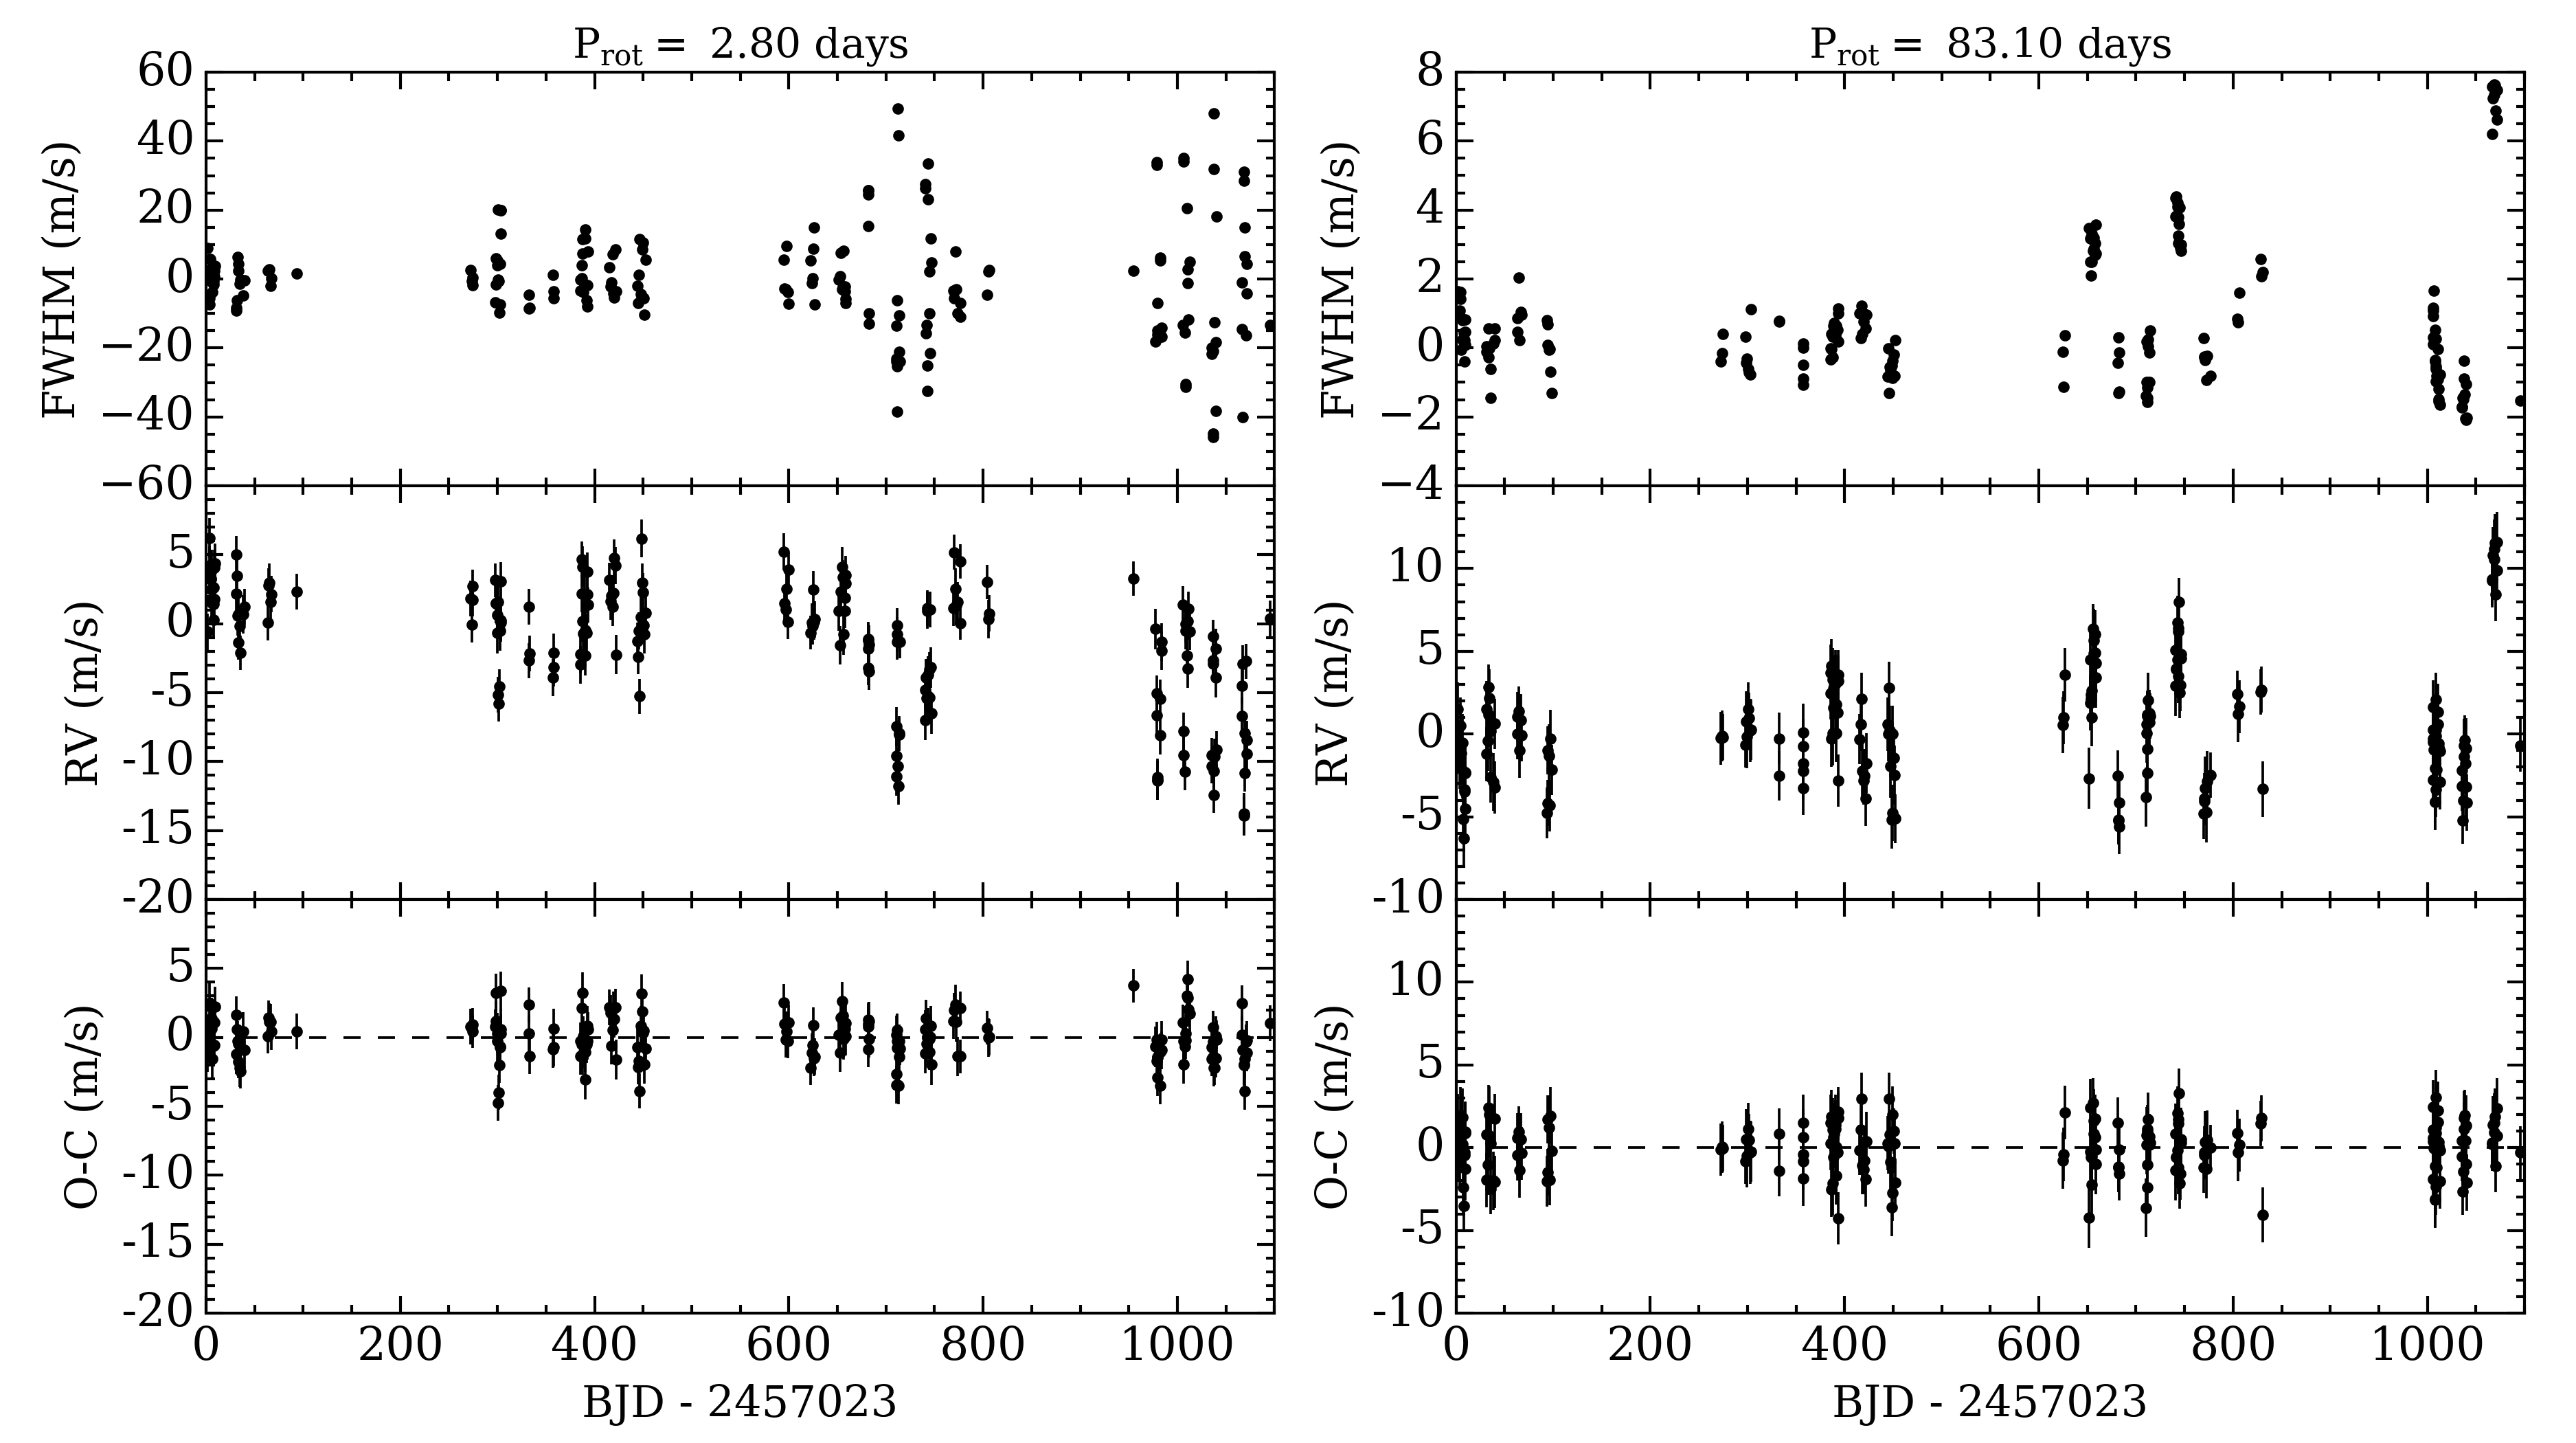
\includegraphics[width=\hsize]{figures/GPexample_bkgd.png}%
  \hspace{-\hsize}%
  \begin{ocg}{fig:GPoff}{fig:GPoff}{0}%
  \end{ocg}%
  \begin{ocg}{fig:GPon}{fig:GPon}{1}%
    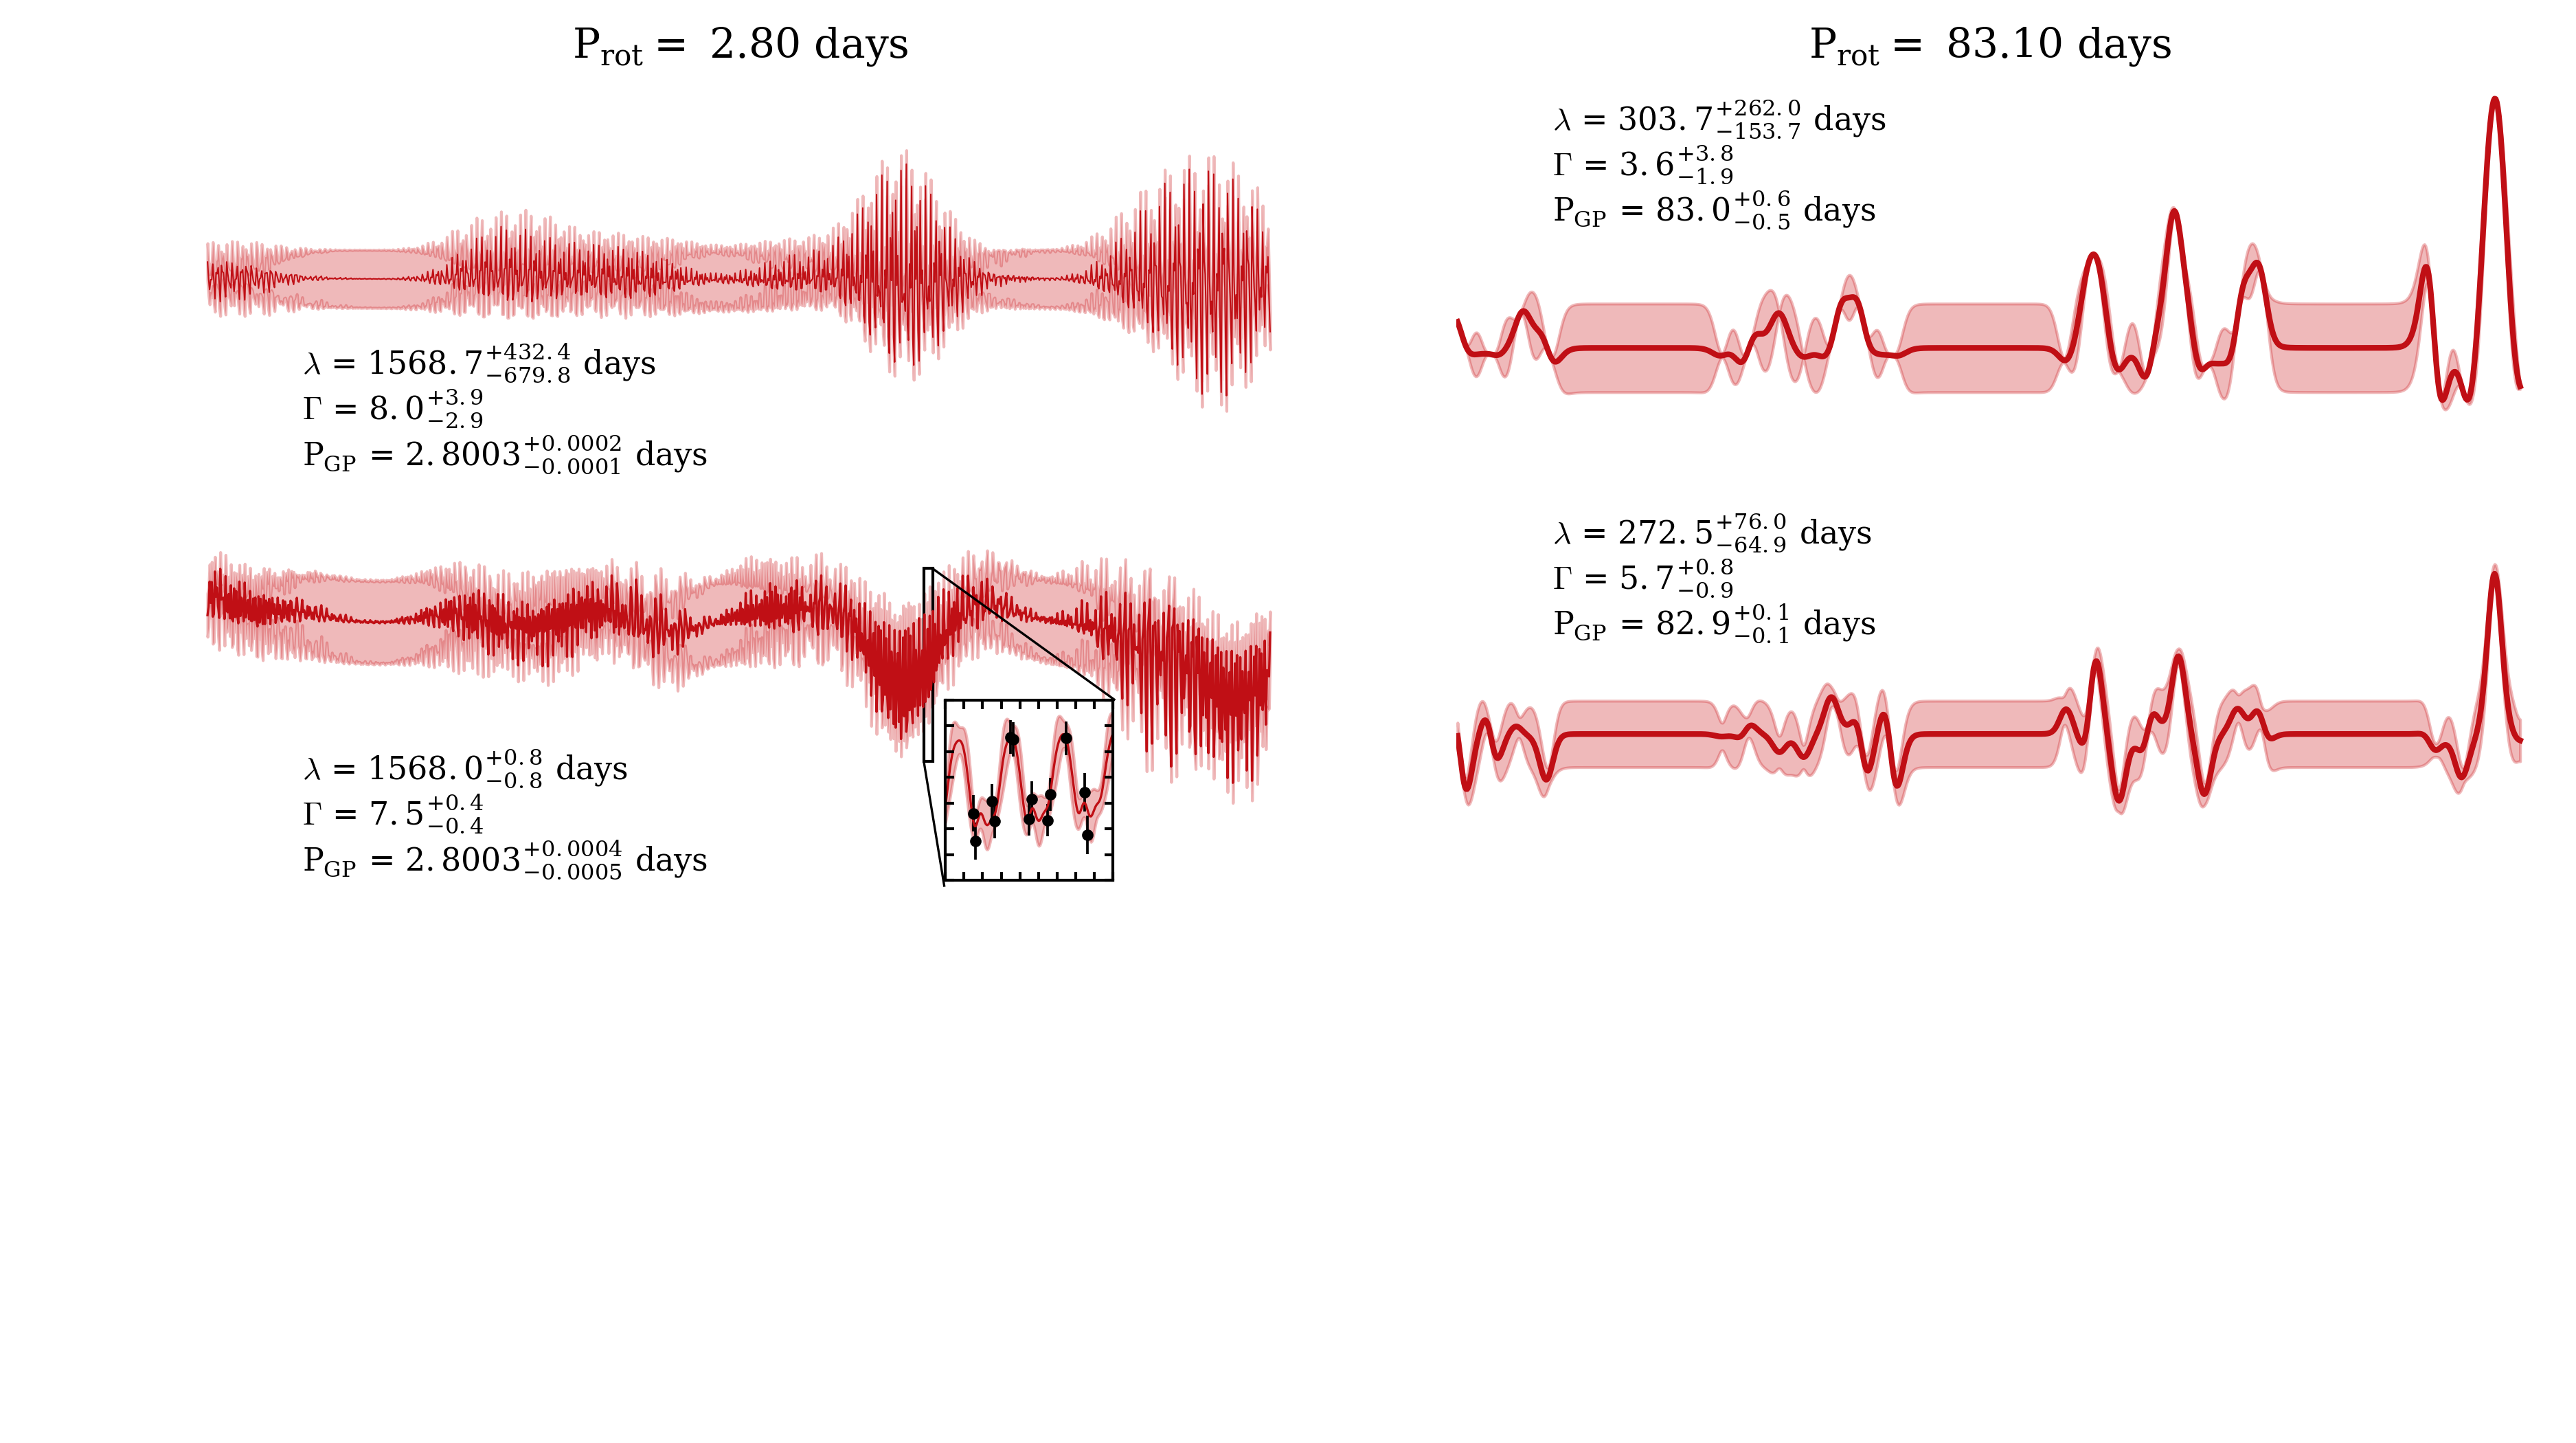
\includegraphics[width=\hsize]{figures/GPexample_GP.png}%
  \end{ocg}
  \hspace{-\hsize}%
  \caption[Examples of GP activity models in simulated SPIRou timeseries.]
      {\small Examples of our GP formalism used to mitigate RV activity and detect underlying planetary signals for two
    simulated systems with either a rapidly (\prot{} $=2.8$ days; \emph{left column}) or slowly (\prot{} $=83.1$ days;
    \emph{right column}) rotating host star. \emph{Top panels}: the FWHM time-series used for training along with the
    \ToggleLayer{fig:GPon,fig:GPoff}{\protect\cdbox{mean GP regression model and its $1\sigma$ confidence interval}}
    shown in red. \emph{Middle panels}: the raw
    RV time-series along with the mean GP activity model (in the absence of planets) and its $1\sigma$ confidence interval.
    \emph{Bottom panels}: the RV residuals after removal of the mean GP activity model shown in the middle panels.
    Each system contains 3 planets which contribute to the $O-C$ residuals albeit with semi-amplitudes which are all
    $\lesssim \sigma_{\text{RV}}$. The two upper rows report the MAP values of GP hyperparameters along with their
    $16^{\text{th}}$ and $84^{\text{th}}$ percentiles.}
  \label{BSfig:GPexample}
\end{figure*}

Following the training phase on the FWHM time-series
we proceed with modelling the RVs simultaneously with a trained GP activity model plus keplerian planetary
signals. The marginalized posterior PDFs of the GP hyperparameters $\lambda$, $\Gamma$, and $P_{\text{GP}}$
from training are used as informative priors in the joint RV analysis which treats the GP amplitude
$a$ as a free parameter. For each assumed mean function $\boldsymbol{\mu}$, containing between zero and three
keplerian solutions, we compute the MAP GP activity model from the hyperparameter values sampled using MCMC.
Assuming a zero mean function, the resulting mean GP activity models
for the two stars shown in Fig.~\ref{BSfig:GPexample} are shown in the middle panels of the figure. The residuals
following the removal of the mean GP activity model is also shown. In each case the stellar rotation period is
detected in the LS periodogram of the FWHM time-series and therefore is used to constrain $P_{\text{GP}}$ during
training. For the rapid rotator with \prot{} $=2.8$ days, the rms of the injected activity is 4.43 \mps{} and
is reduced to 1.59 \mps{} after removing the mean GP activity model ($\chi_{\text{red}}^2 =1.4$ for four GP hyperparameters).
This resulting RV rms is more comparable
to the median RV measurement uncertainty $\sigma_{\text{RV}}=1.35$ \mps{.} In the slow rotator case (\prot{} $=83.1$ days)
the rms of the injected activity is reduced from 3.60 \mps{} to 1.53 \mps{} compared to
$\sigma_{\text{RV}}=1.63$ \mps{} ($\chi_{\text{red}}^2 =0.9$). In both test cases considered in
Fig.~\ref{BSfig:GPexample}, a planet is detected in the RV residuals and fit simultaneously with the activity assuming
a new mean model containing a single keplerian solution. Details of our planet detection algorithm are discussed in
Sect.~\ref{BSsect:detection}.


\subsection{GP Activity Model Performance}
As an overview of the performance of our GP activity modelling, we can compare the rms of the known
injected RV activity with the rms of the residuals following the removal of our mean GP activity model. The residual
rms should never exceed the rms of the injected activity otherwise our GP formalism would be adding additional noise
into the RV time-series rather than modelling and reducing it as is its intended purpose. Similarly, optimal GP fits
will result in a residual rms that is close to the median RV measurement uncertainty of the time-series. \\

Fig.~\ref{BSfig:compareGPres} compares the rms of the \emph{injected} RV activity to the rms of the \emph{residual} RV activity
after removing the mean GP activity model computing assuming a zero planet model. Recall that we only compute a GP activity model
when the injected rms is $> \sigma_{\text{RV}}$ such that the injected activity rms in units of $\sigma_{\text{RV}}$
is always greater than or equal to unity in Fig.~\ref{BSfig:compareGPres}.
We note that the residual activity rms never exceeds the injected activity rms as expected; i.e. the residual rms
always lies beneath the line $y=x$ in Fig.~\ref{BSfig:compareGPres}. Secondly,
there appears to be a positive correlation between \prot{} and the relative reduction of the activity rms,
which is analogous to GP performance. That is that within our sample of RV time-series which are modelled with a GP activity
model, the activity rms is maximally reduced in systems
with the longest rotation periods. Conversely, the GP performance when applied to rapid rotators (\prot{} $\gtrsim 2$ days)
is often marginal in comparison. The exact cause of these effects above may be related to the poor time-sampling of our
observations compared to the short stellar rotation period but is ultimately beyond the scope of this paper and is reserved
for a future study. \\

\begin{figure}
  \centering
  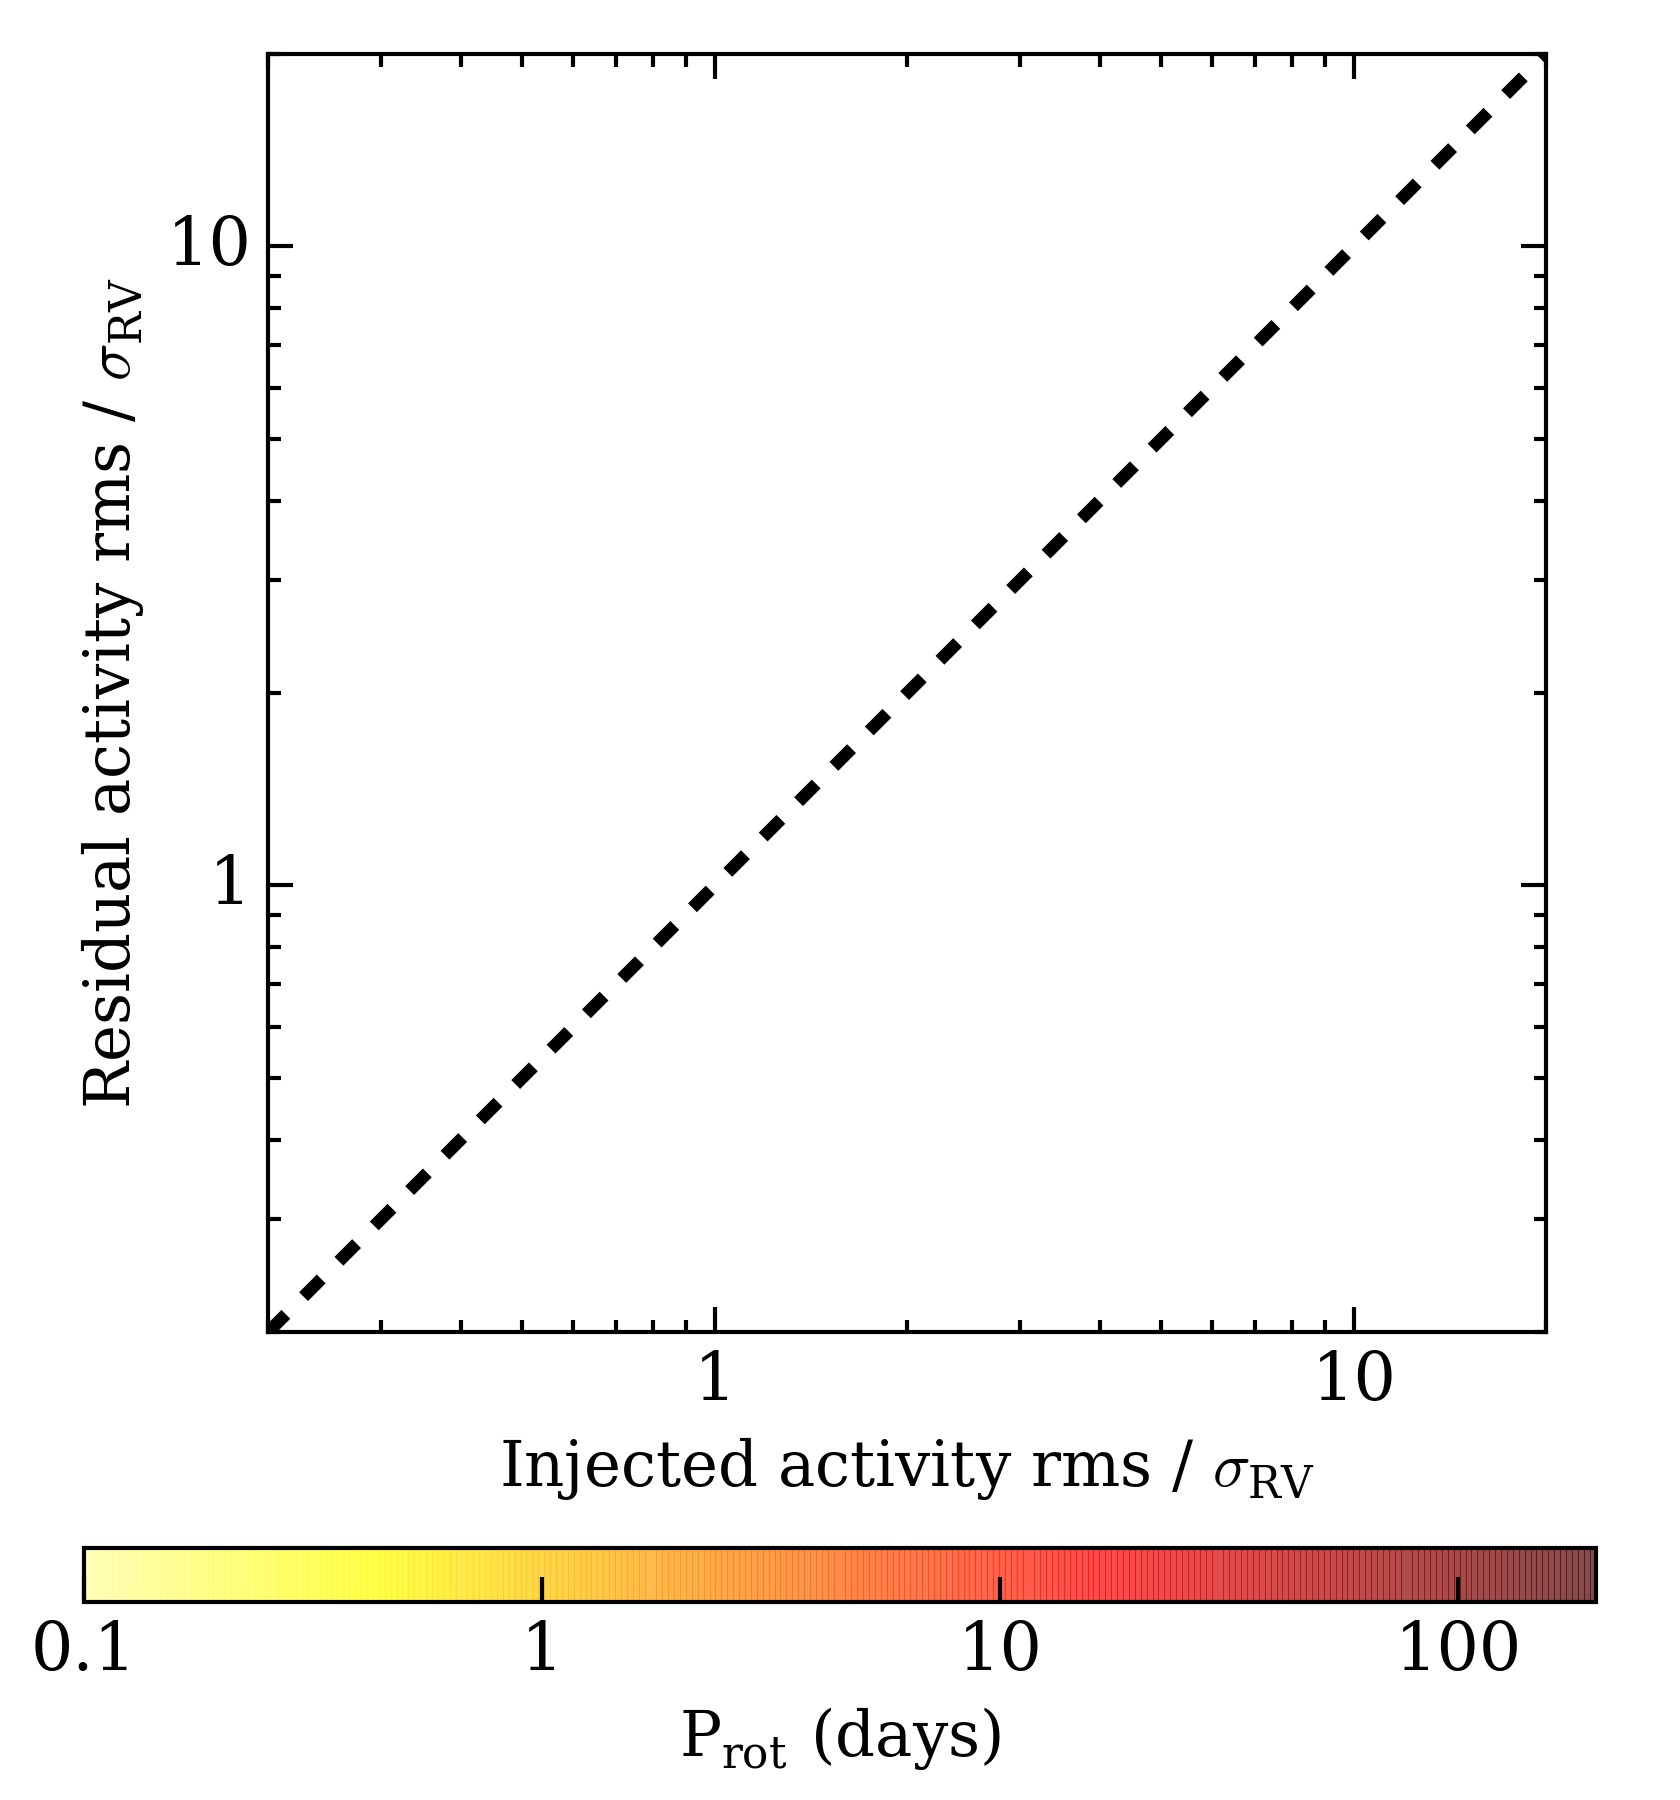
\includegraphics[width=0.6\hsize]{figures/compareGPres_bkgd.png}%
  \hspace{-0.6\hsize}%
  \begin{ocg}{fig:detoff}{fig:detoff}{0}%
  \end{ocg}%
  \begin{ocg}{fig:deton}{fig:deton}{1}%
   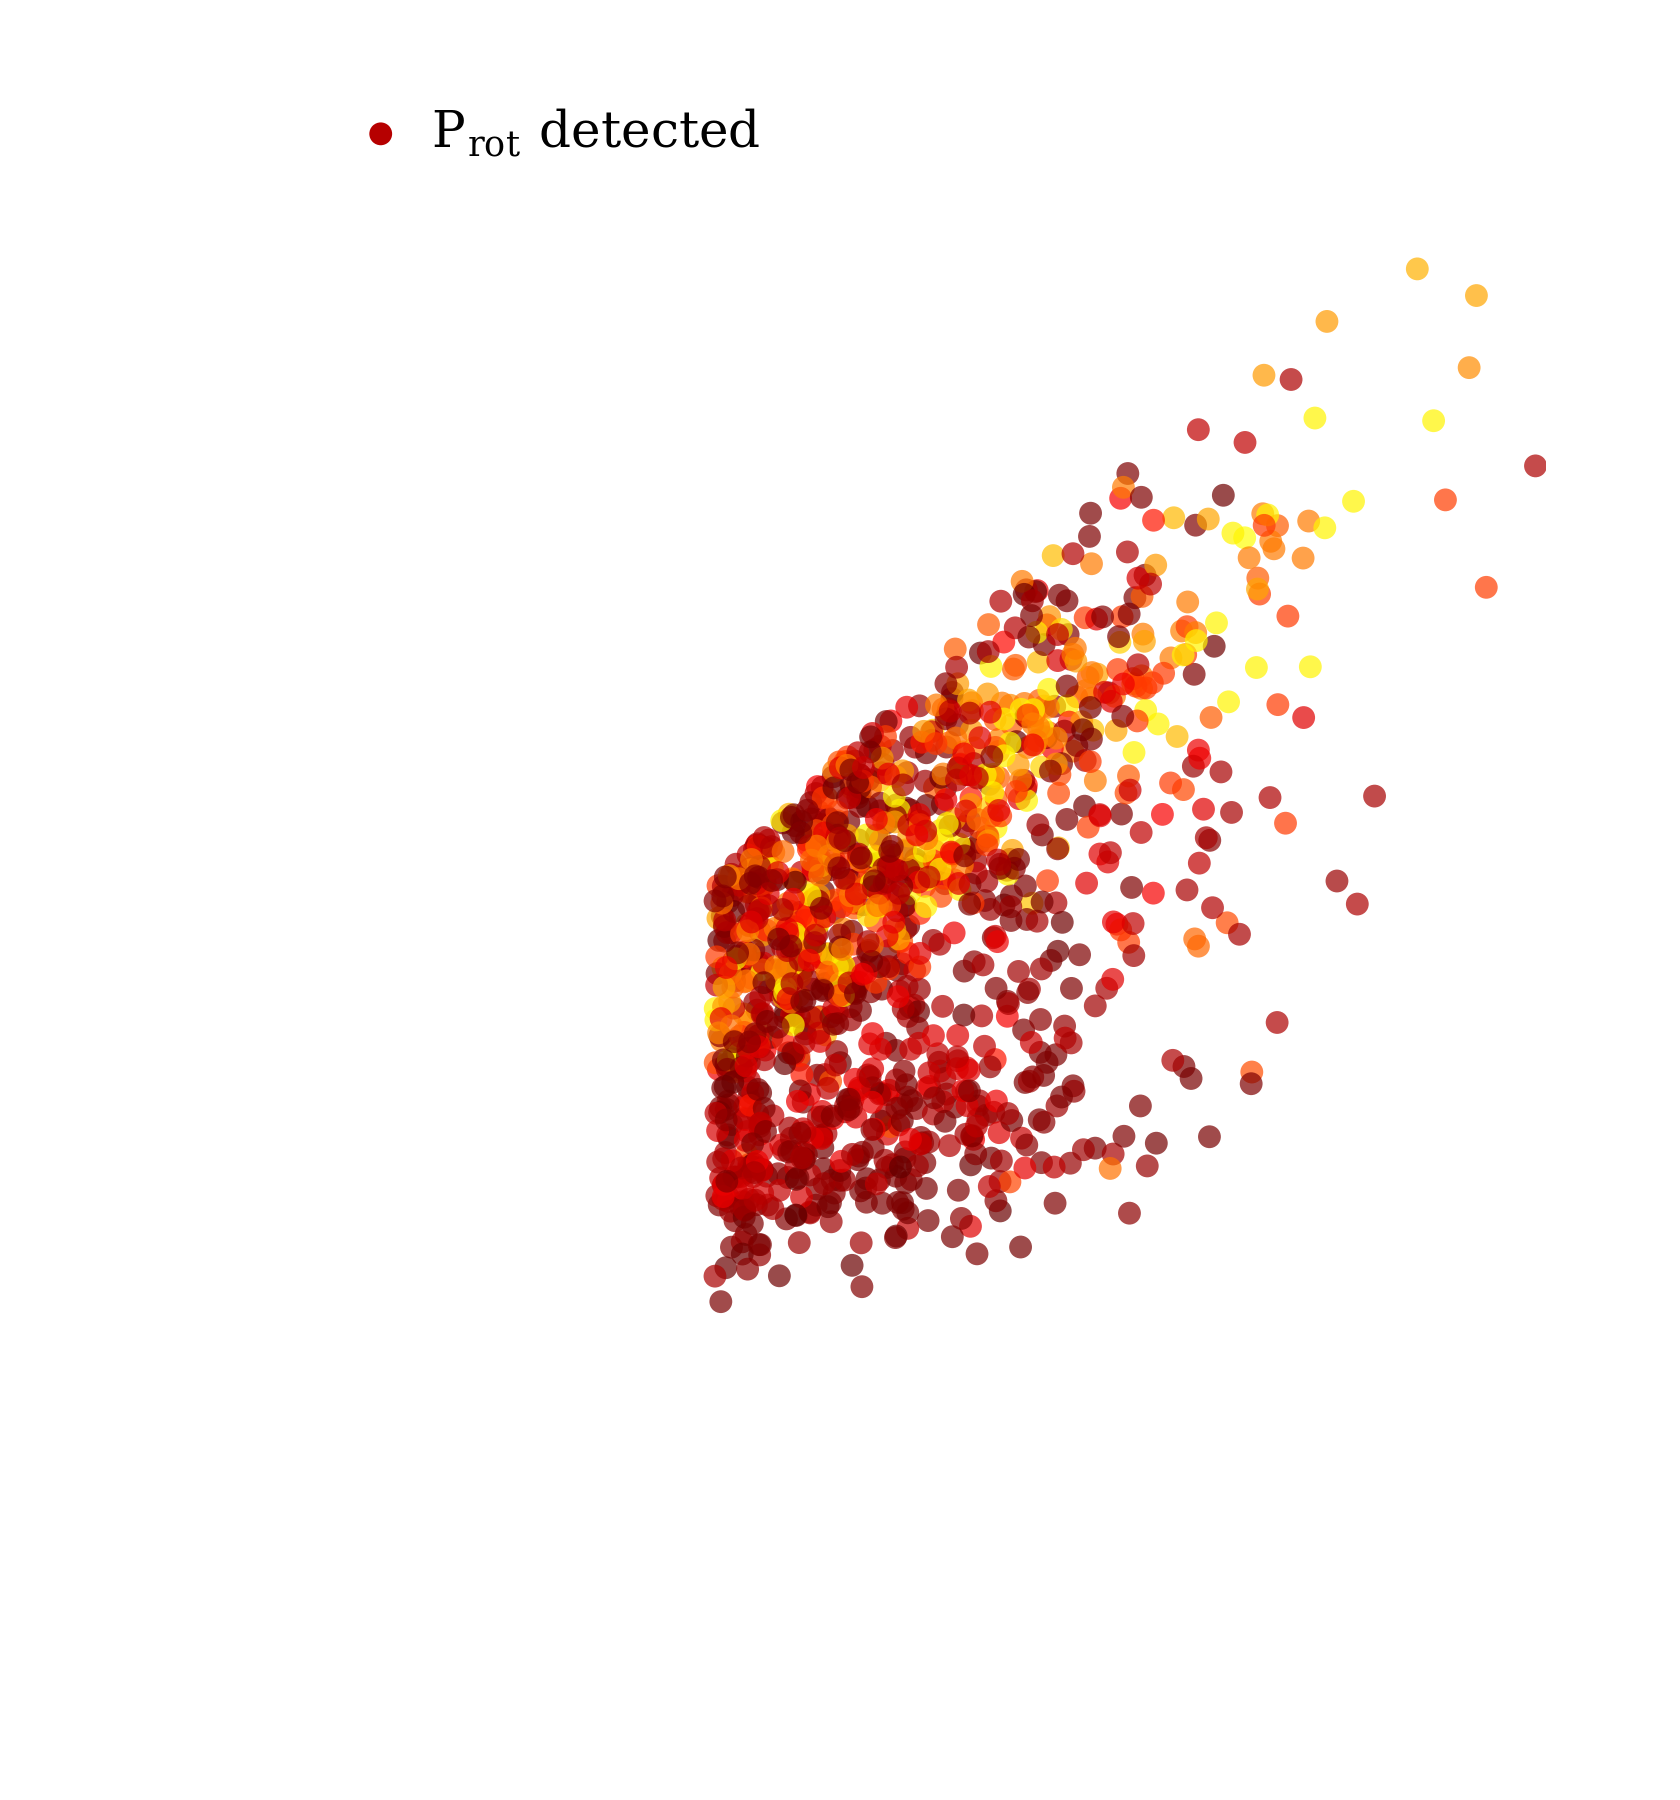
\includegraphics[width=0.6\hsize]{figures/compareGPres_det.png}%
  \end{ocg}
  \hspace{-0.6\hsize}%
  \begin{ocg}{fig:nondetoff}{fig:nondetoff}{0}%
  \end{ocg}%
  \begin{ocg}{fig:nondeton}{fig:nondeton}{1}%
   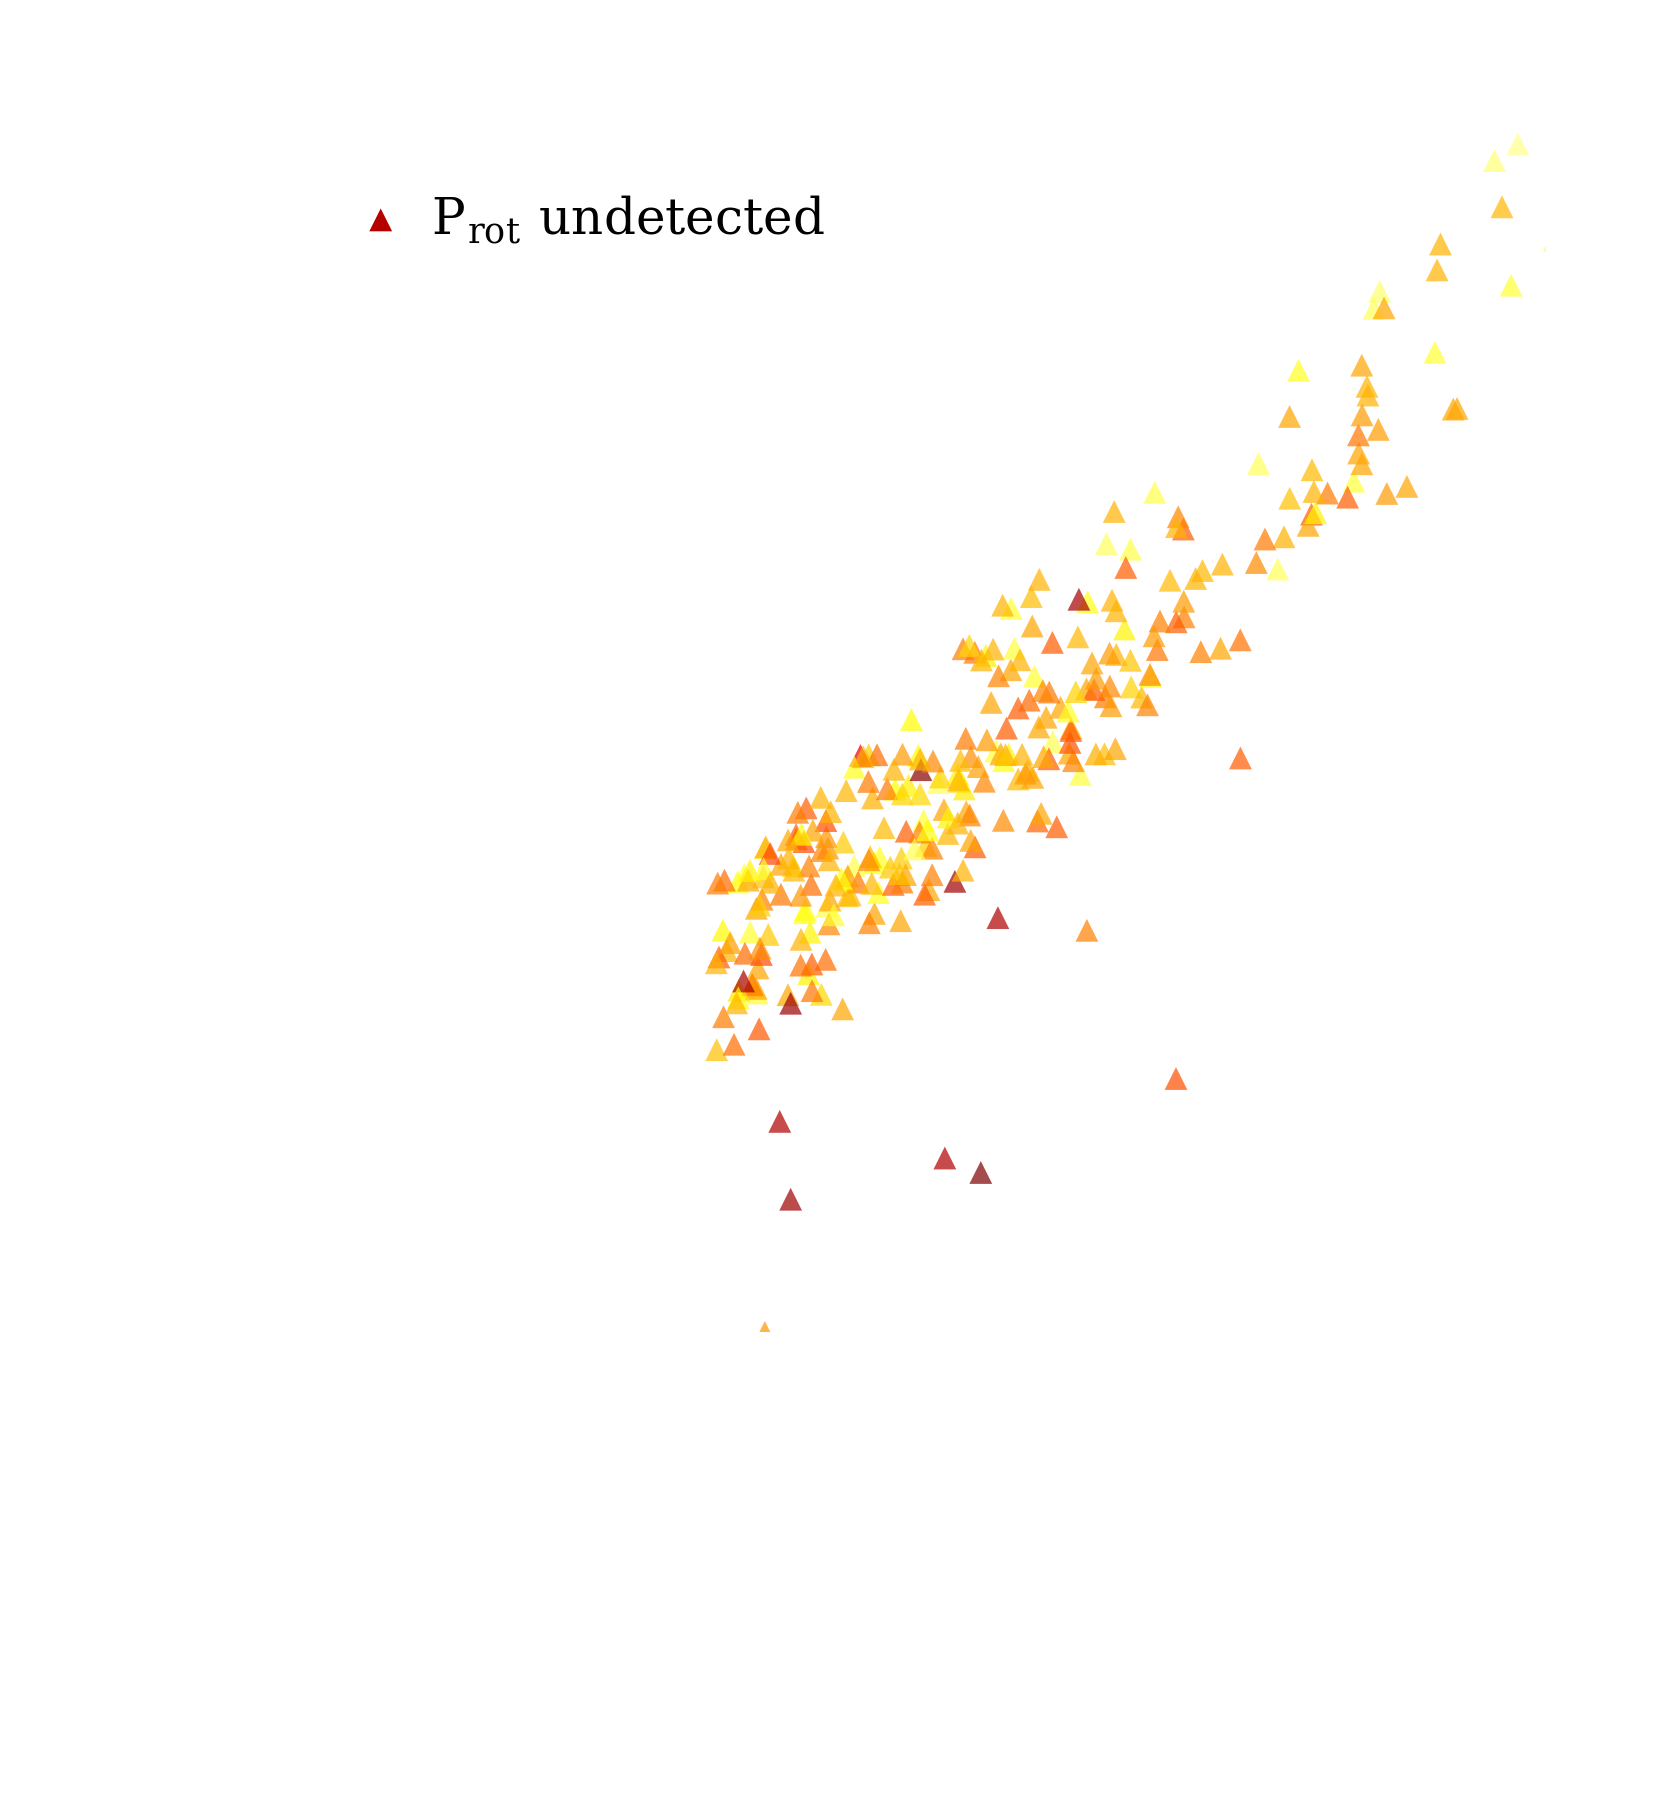
\includegraphics[width=0.6\hsize]{figures/compareGPres_nondet.png}%
  \end{ocg}
  \hspace{-0.6\hsize}%
  \caption[GP activity model performance in simulated SPIRou RV timeseries.]
    {\small Comparison of the rms of the \emph{injected} RV activity to the rms of the \emph{residual} RV activity following
    the removal of the mean GP activity model which is
    computed in the absence of planets. Each rms value is normalized by the
    RV measurement uncertainty $\sigma_{\text{RV}}$ of its time-series. The \emph{dashed line} $y=x$ is indicative of cases
    wherein the GP activity model does not reduce rms due to activity. Time-series in which \prot{} is detected in the
    FWHM time-series are depicted as 
    \ToggleLayer{fig:deton,fig:detoff}{\protect\cdbox{\emph{circles}}}. Whereas time-series in which \prot{} is not detected in
    the FWHM times-series are depicted as \ToggleLayer{fig:nondeton,fig:nondetoff}{\protect\cdbox{\emph{triangles}}}.}
  \label{BSfig:compareGPres}
\end{figure}

We note that in many slow rotator cases, the dimensionless residual rms is often less than unity. This suggests that in such
cases the non-parametric GP is actually modelling the noise and not just the stellar activity signal.
Unfortunately when the GP activity model is over-fitting the RV noise, planetary signals can be absorbed into the mean GP
model and thus avoid detection. Furthermore,
this apparent over-fitting is a common feature in many of our simulations and does not appear to depend on
whether or not the stellar rotation period is detected a-priori in the FWHM time-series.
However it is true that on average,
the GP modelling out-performs cases in which \prot{} is known from the FWHM compared to cases in which \prot{} remains
undetected thus providing very weak constraints on $P_{\text{GP}}$.
This highlights the importance having a-priori knowledge of \prot{} from any of the
ancillary spectroscopic times-series, polarimetric time-series \citep{hebrard16},
or from previously obtained long-baseline photometry \citep[e.g.][]{newton16a}.


\section{Automated Planet Detection} \label{BSsect:detection}
Due to the large number of planetary systems in our simulated SLS-PS, we must detect planets in an automated
way. The steps in our automated planet detection algorithm
represent computationally tractable calculations given the large number of planetary systems
for which each step must be performed. We note however that other---potentially more robust---planet
detection algorithms may be adopted in the real SLS-PS which are likely to include more
human intervention than the automated techniques described in the following subsections.

\subsection{Establishing Putative Planetary Detections} \label{BSsect:det}
We proceed by searching for planetary periodicities in an iterative manner using the LS periodograms
of the RVs following the removal of various periodic signals.
An example of this iterative process is visualized in Fig.~\ref{BSfig:periodograms} for a 3 planet system
($P_b,P_c,P_d=1.85,7.17,14.66$ days, $K_b,K_c,K_d=4.7,2.3,0.07$ \mps{} respectively)
around a moderately active star with a measured photometric rotation period \prot{} $\sim 8.8$ days and
an RV rms in the absence of planets of $\sim 4.2$ \mps{.} \\

For MC realizations in which the rms of the injected RV activity exceeds the median RV measurement
uncertainty---as is the case for the system shown in Fig.~\ref{BSfig:periodograms}---we compute two
versions of our initial periodogram: one of the raw RVs \emph{only} and a second
of the RV residuals after fitting the data with the trained GP activity model and zero mean function
(i.e. no planet model). This GP model predicts the RV activity in the absence of planetary signals.
For the remaining MC realizations containing quiet stars
we only compute the LS periodogram of the raw RVs thus neglecting any
modelling of correlated RV residuals. For cases in which we use a trained GP to model RV activity,
it is beneficial for
the periodic term of the assumed quasi-periodic covariance kernel to be constrained by our training set.
For the example shown in Fig.~\ref{BSfig:periodograms}, the top panel shows the LS periodogram of the FWHM
in which \prot{} is detected and is subsequently used in our RV modelling (see Sect.~\ref{BSsect:regression}). \\

\begin{figure}
  \centering
  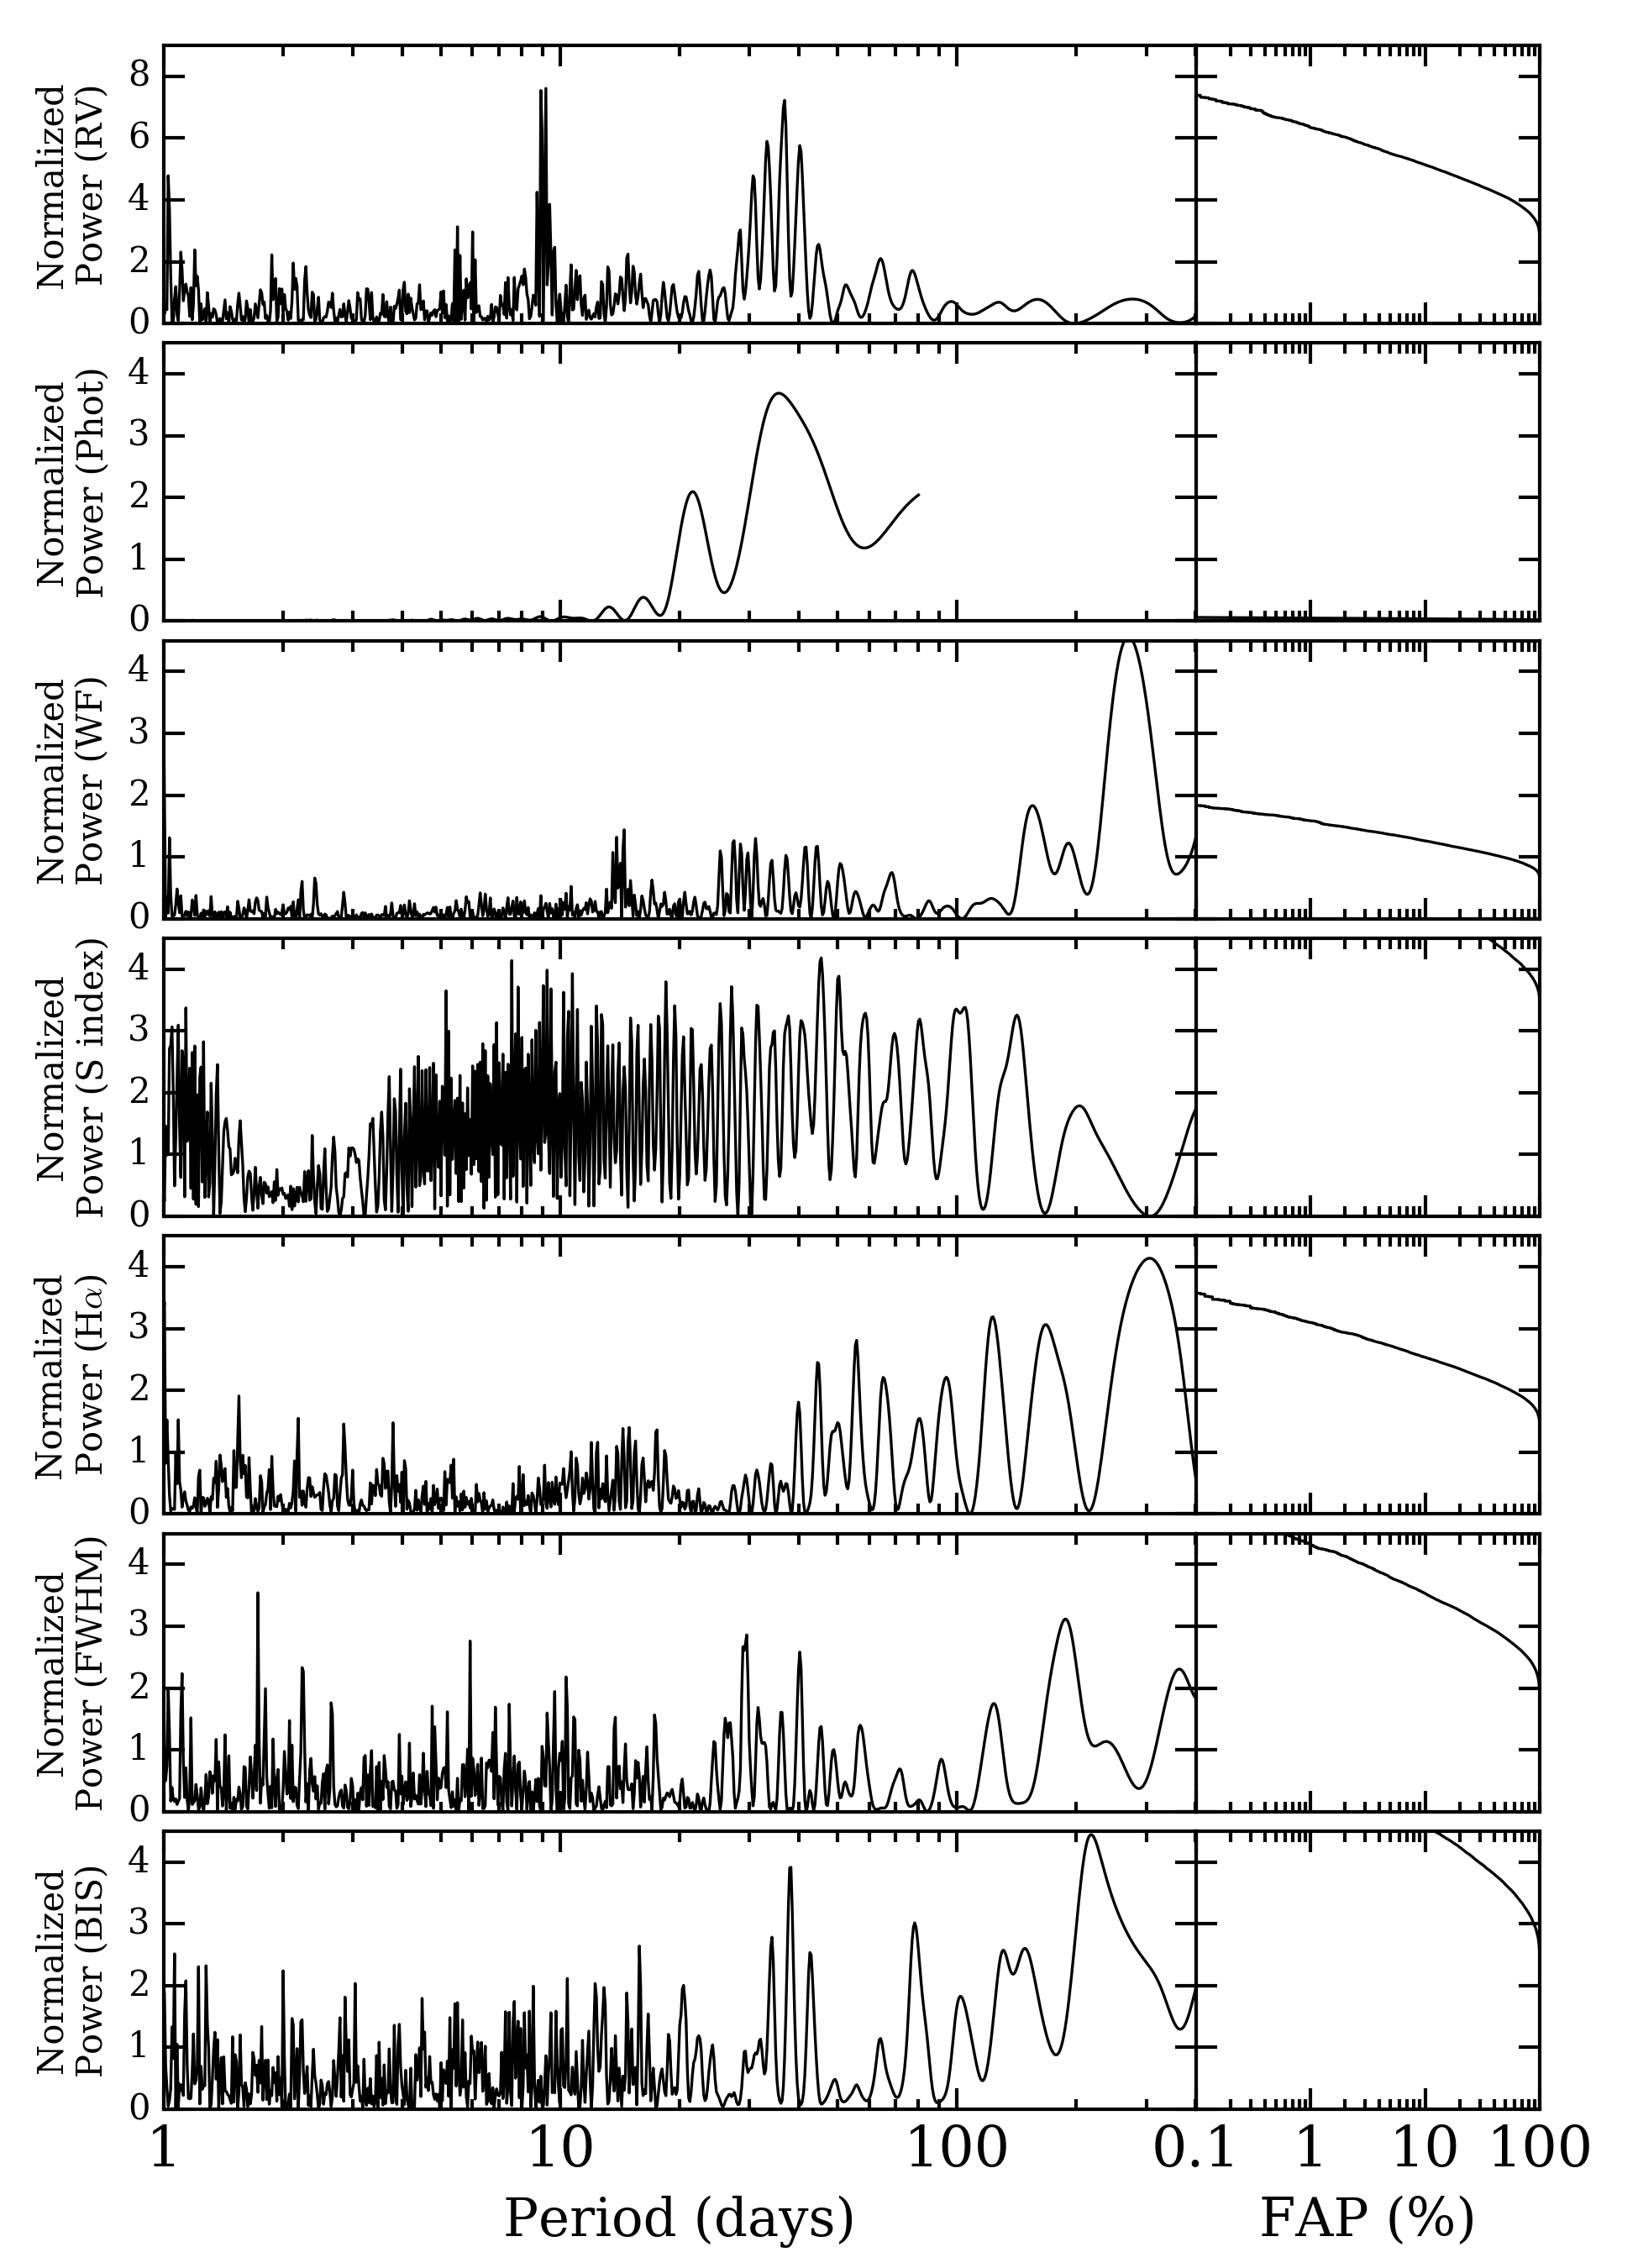
\includegraphics[width=0.8\hsize]{figures/periodograms_bkgd.png}%
  \hspace{-0.8\hsize}%
  \begin{ocg}{fig:Poff}{fig:Poff}{0}%
  \end{ocg}%
  \begin{ocg}{fig:Pon}{fig:Pon}{1}%
    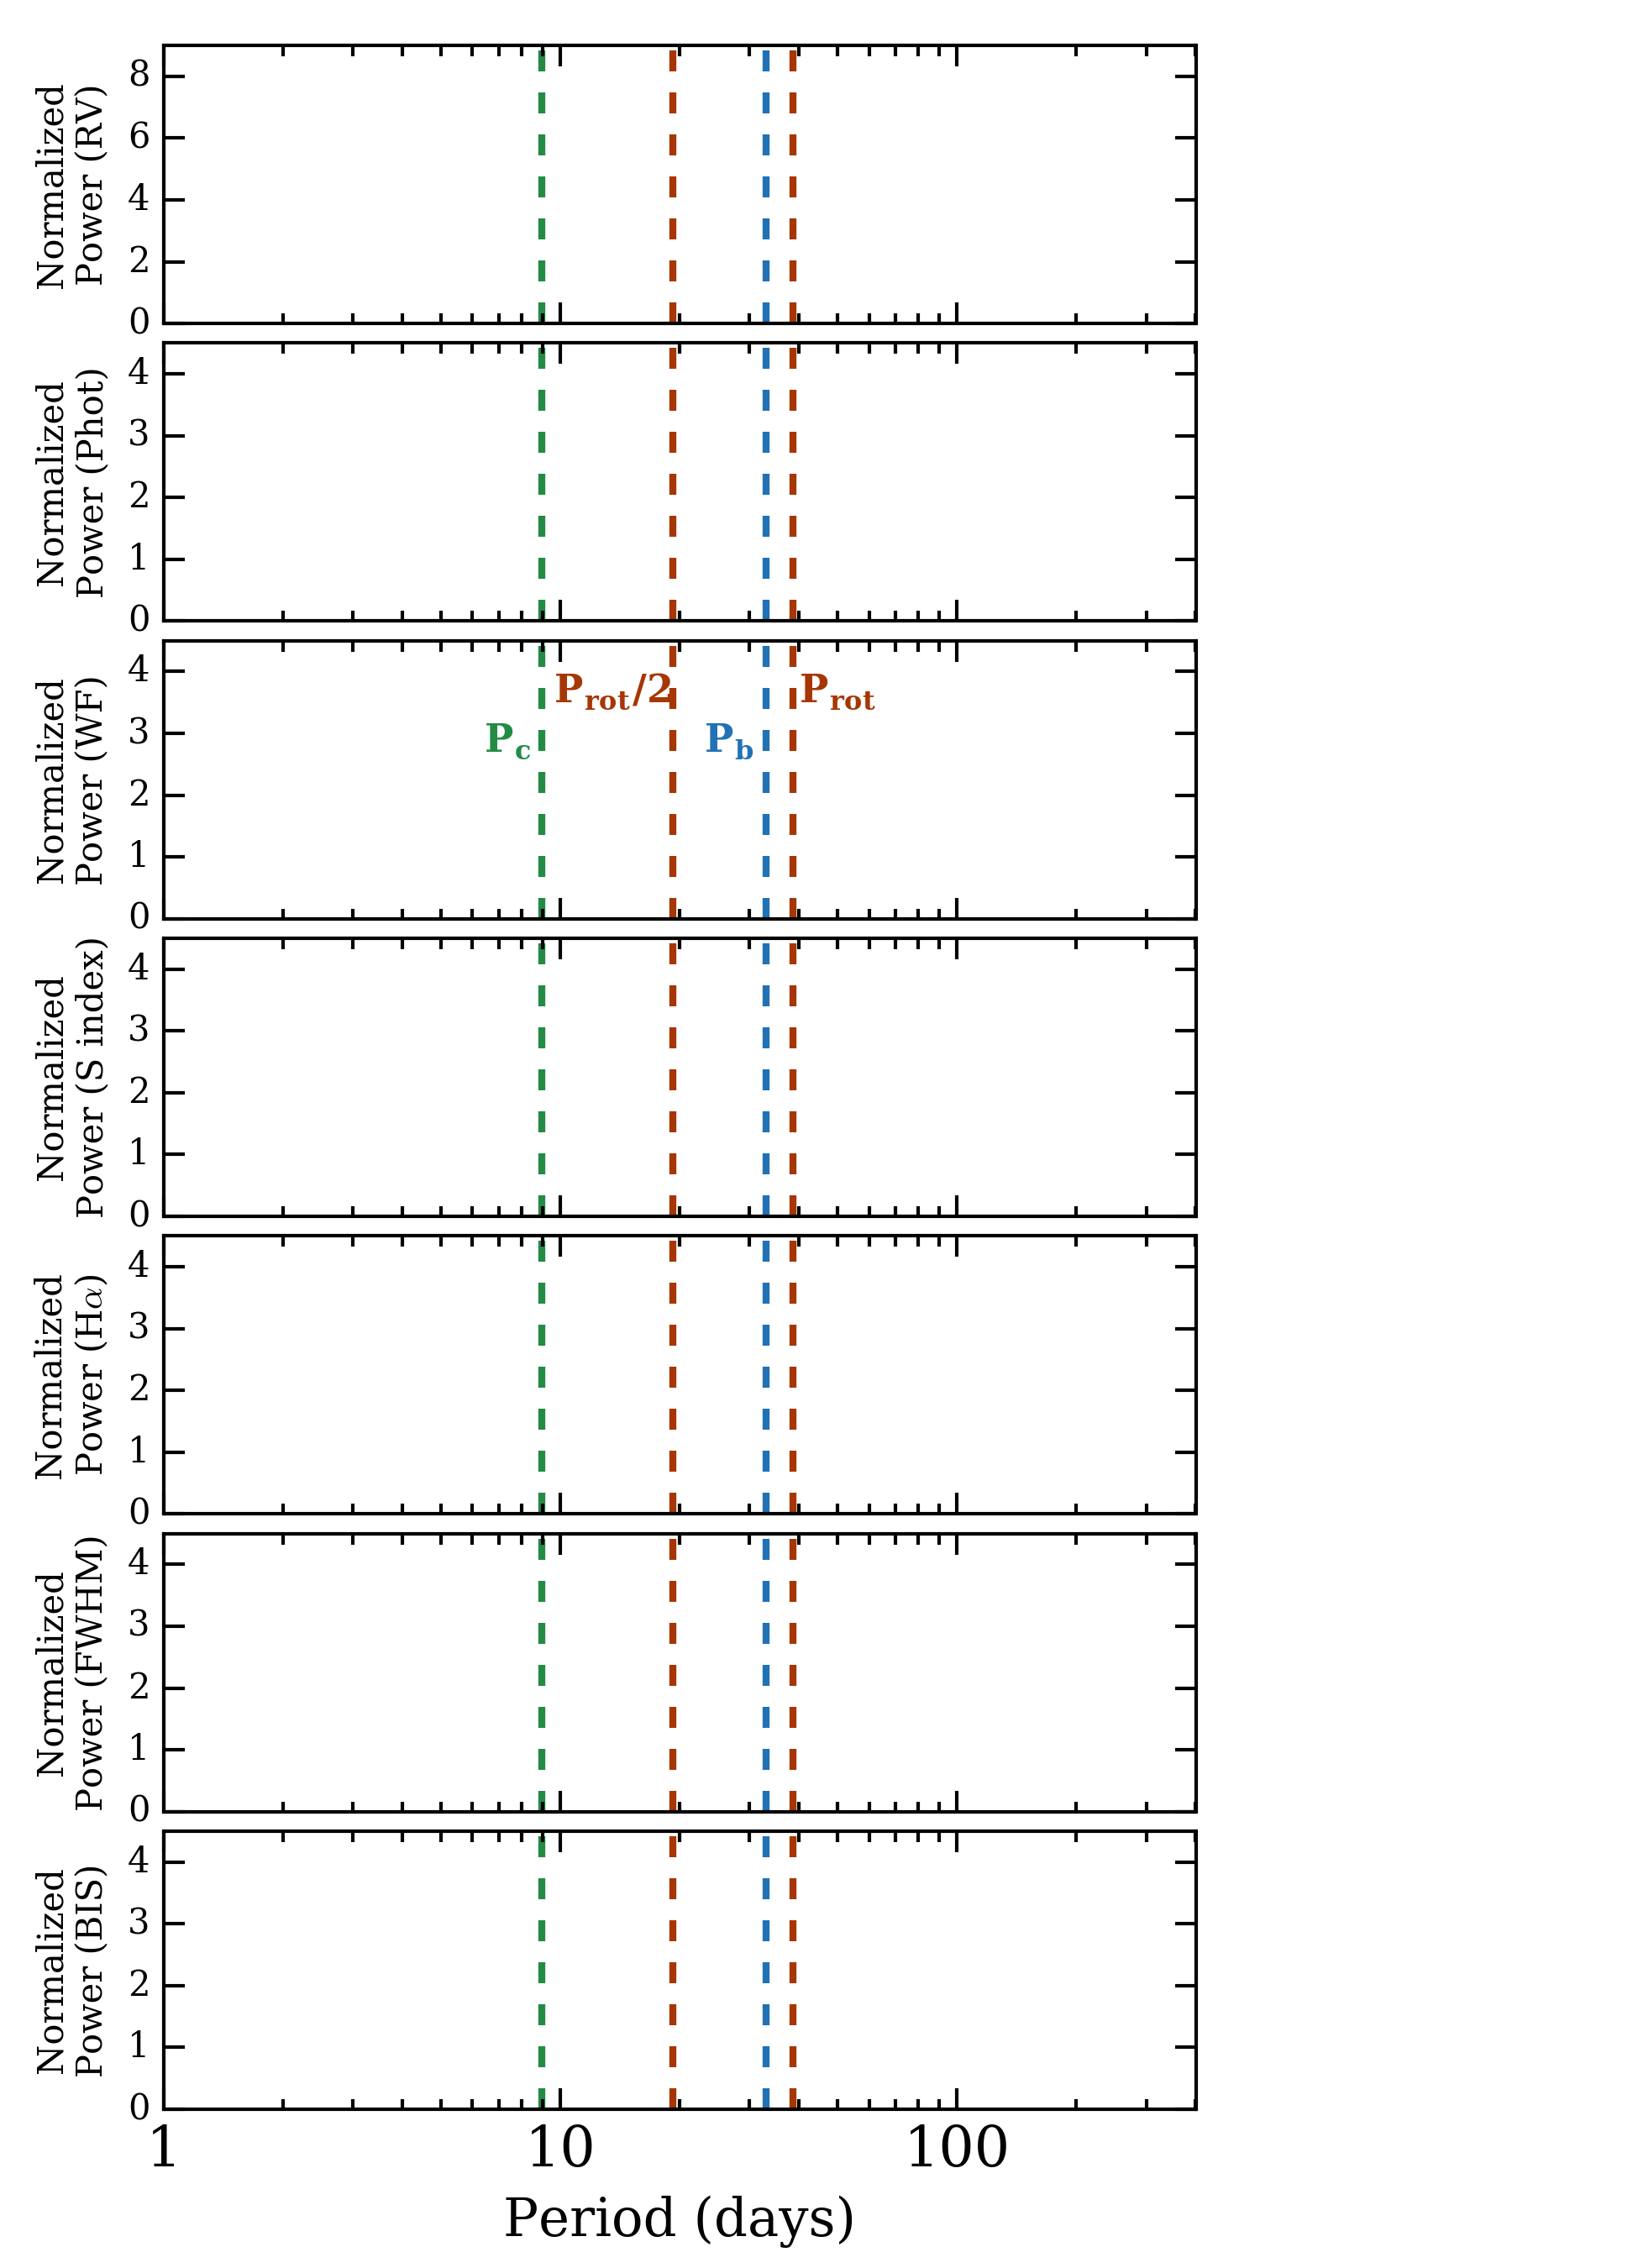
\includegraphics[width=0.8\hsize]{figures/periodograms_Ps.png}%
  \end{ocg}
  \hspace{-0.8\hsize}%
  \begin{ocg}{fig:FAPoff}{fig:FAPoff}{0}%
  \end{ocg}%
  \begin{ocg}{fig:FAPon}{fig:FAPon}{1}%
    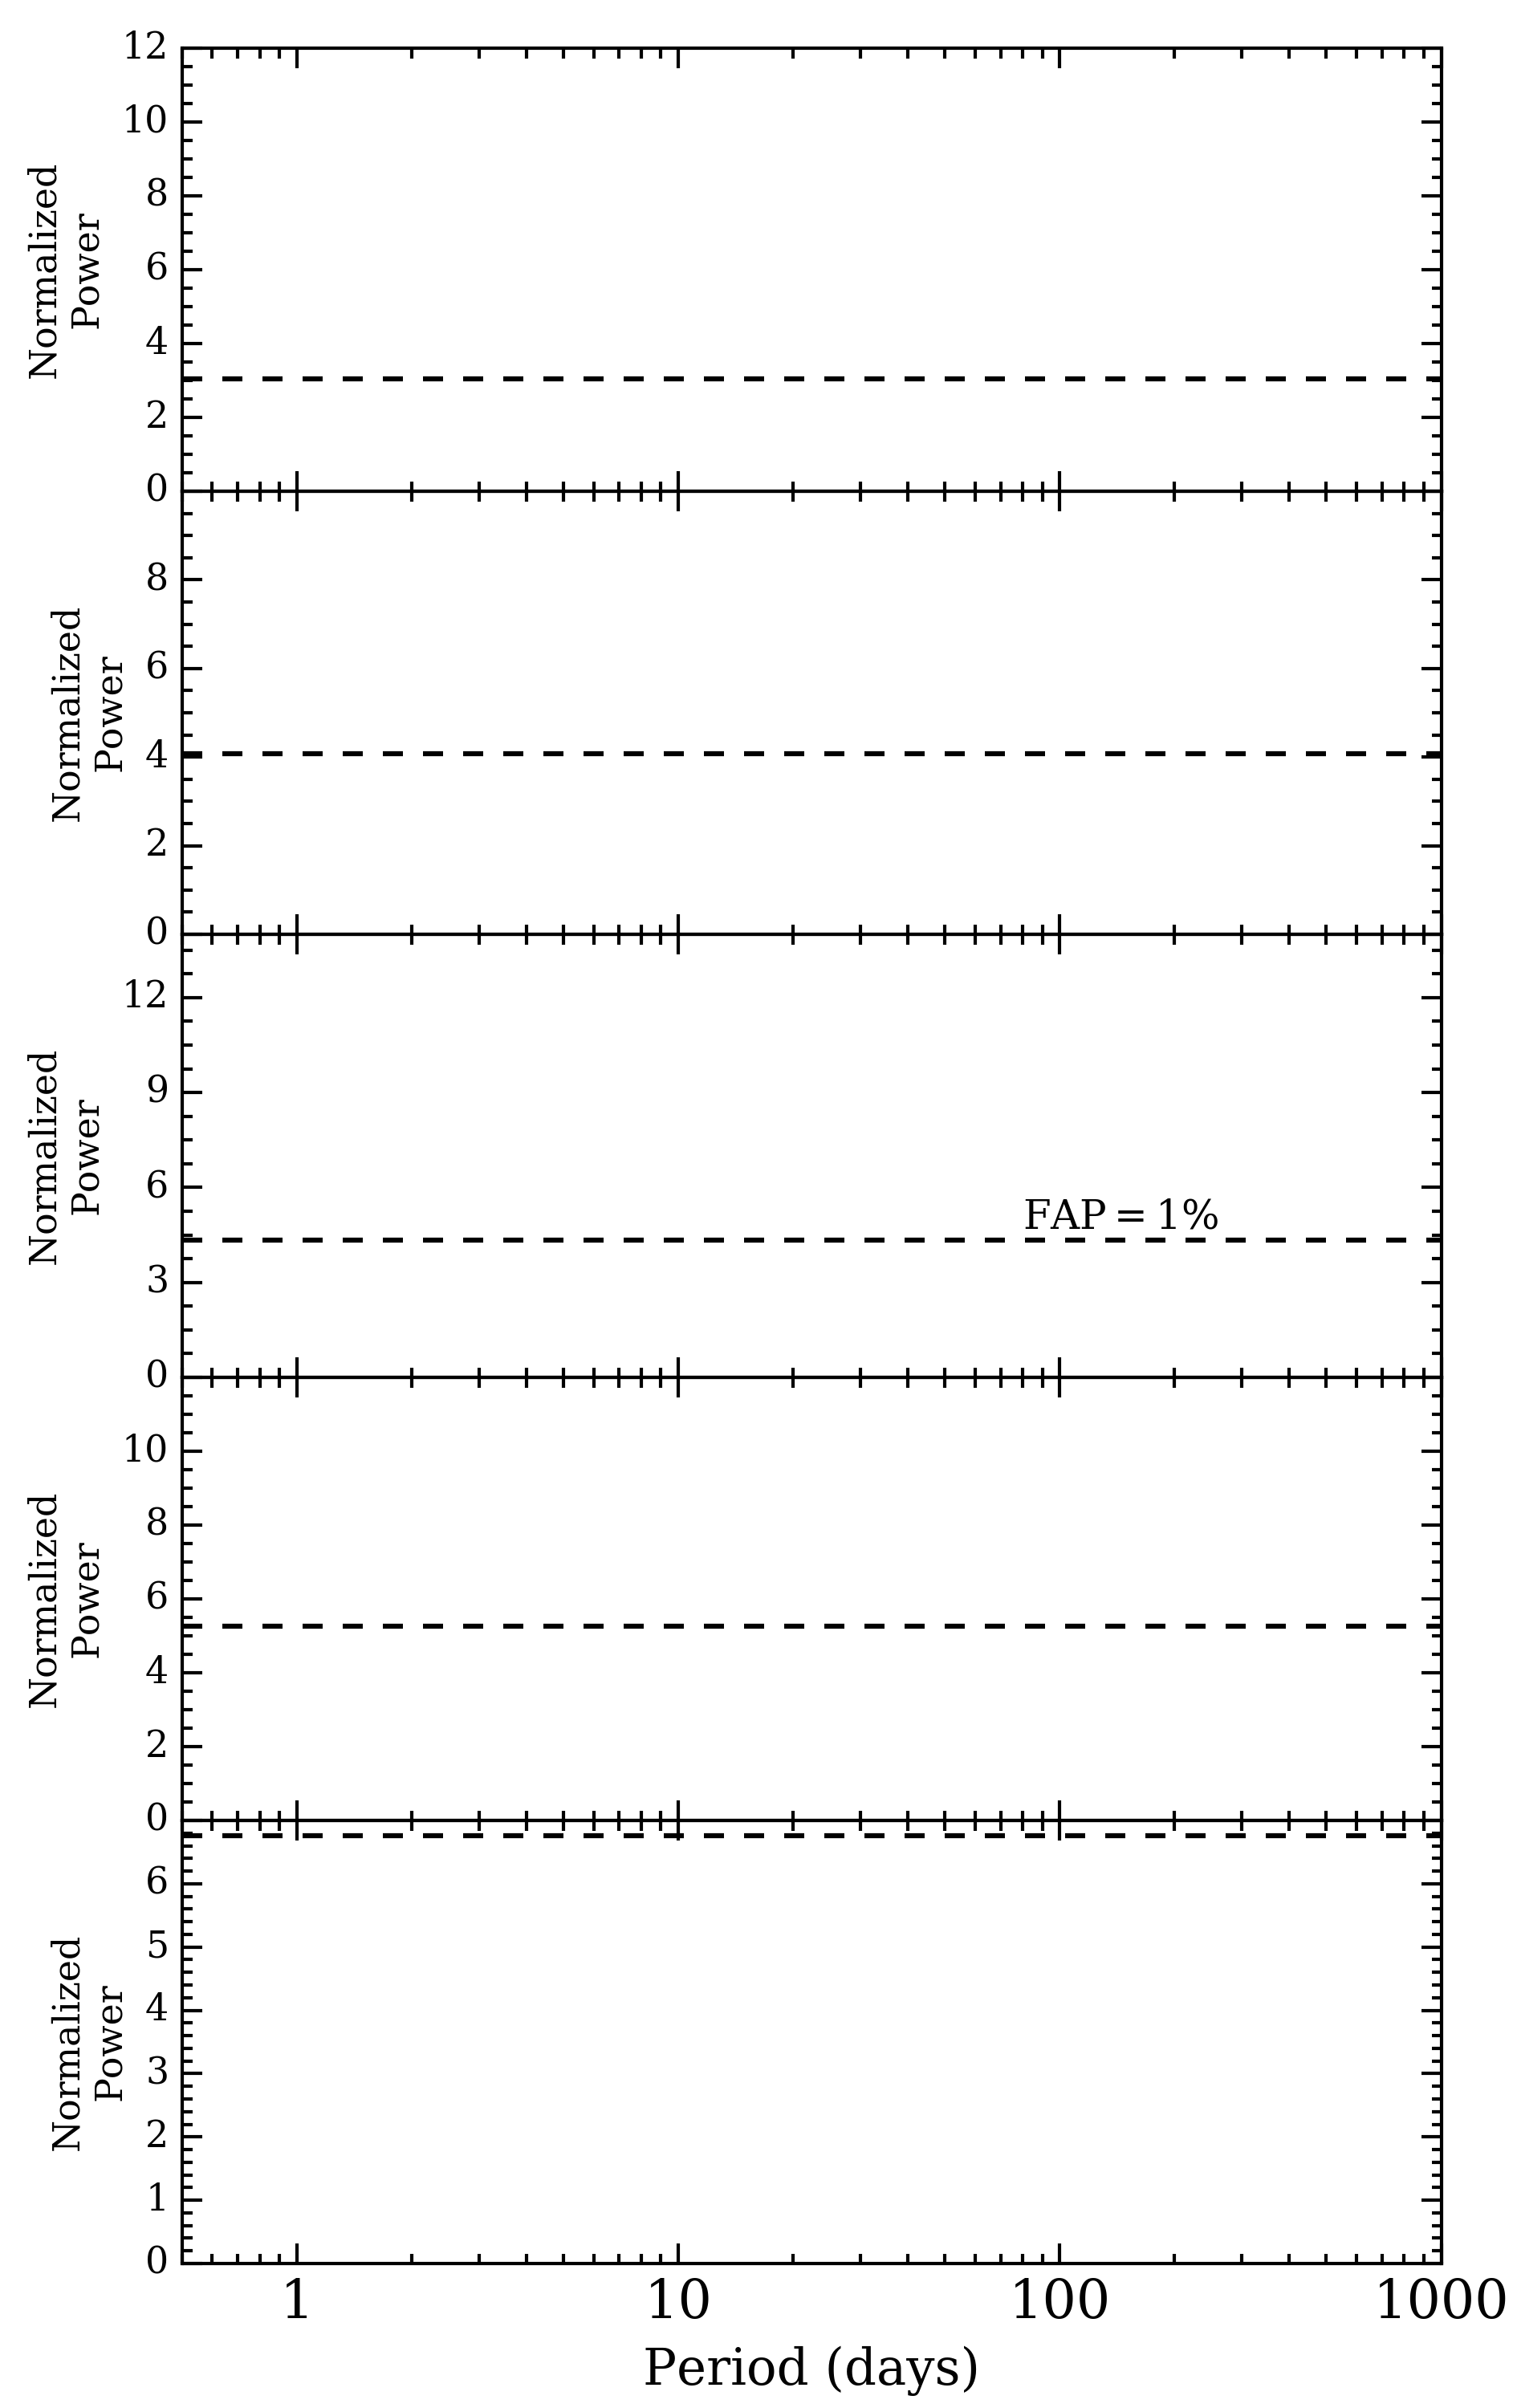
\includegraphics[width=0.8\hsize]{figures/periodograms_FAP.png}%
  \end{ocg}
  \hspace{-0.8\hsize}%
  \caption[Illustrating the iterative planet search with Lomb-Scargle periodograms.]
      {\small \emph{Top to bottom}: Lomb-Scargle periodograms of the full width at half maximum (FWHM)
    of the cross-correlation function, raw radial velocities (RVs), RVs corrected for activity (RVs-GP),
    RVs corrected for activity and a planet (RVs-GP-b), and the RVs corrected for activity and two planets
    (RVs-GP-b-c). Periodicities equal to the stellar rotation period, its first harmonic, and the
    orbital periods of the three planets in the system are highlighted with
    \ToggleLayer{fig:Pon,fig:Poff}{\protect\cdbox{\emph{vertical lines}}}. The power
    corresponding to a 1\% false alarm probability in each periodogram is highlighted by a  
    \ToggleLayer{fig:FAPon,fig:FAPoff}{\protect\cdbox{\emph{horizontal dashed line}}} in each panel.}
  \label{BSfig:periodograms}
\end{figure}

The second panel in Fig.~\ref{BSfig:periodograms} depicts the LS periodogram of the raw RVs only whereas
the third panel depicts the raw RVs corrected by the trained GP activity model with
$P_{\text{GP}}=P_{\text{rot}}=8.8$ days. Comparing these two periodograms it is apparent
that some power at \prot{} is diminished when removing the mean GP activity model
along with power at long periods due to the large exponential
timescale found during training. More importantly, the strongest periodic signal in each periodogram is
at the orbital period of the innermost planet at $\sim 1.85$ days suggesting the presence of a
planet. In these periodograms, and in all subsequent iterations, we claim a putative planet detection
for periodicities with i) FAP $\leq 1$\% ii) is within 2\% of an injected planet's orbital period iii)
is not associated with significant
periodic signals seen in the FWHM time-series iv) is not an alias of the time-sampling (see example in
Fig.~\ref{BSfig:wfs})
and v) is $>2$\% away from the stellar rotation period and any of its first four harmonics. The signals
at $\sim 1.85$ days in the second and third panels of Fig.~\ref{BSfig:periodograms} obey these criteria and
therefore constitute a putative planet detection. We proceed by referring to this putatively
detected planet as `b'. \\

We note that the second condition for a putative planet detection above cannot be utilized in a real survey
because any planetary periodicities are not known a-priori. Instead we invoke this condition to
accelerate our automated planet detection algorithm relative to the steps that must be taken in a real survey
to secure planet detections \citep[e.g. Bayesian model comparison;][]{ford07}.
Without a-priori knowledge of planet orbital periods, LS periodicities at high
significance that obey all of the remaining aforementioned putative planet criteria, may represent false positive
signals if not carefully modelled.
In our simulations we find that on average our time-series generate $\sim 0.5$ such false positives in their LS
periodograms following the removal of planet models. Although
a fraction of these false positive periodicities are likely to be aliases of each other making the above
estimate an upper limit. Ideally the determination of these signals as false positives or as true planetary
signals would be solved via a formal model comparison in a subsequent analysis. However, such calculations are
not guaranteed to converge to the correct solution \citep[see][]{dumusque17}. \\

The second periodogram iteration requires that we fit the putative planetary signal and search for
additional signals in the LS periodogram of the residuals. To model planet `b'
we adopt the maximum-likelihood keplerian model parameters at the detected periodicity
and re-compute the GP activity model which is modified due to the new mean function (i.e. a one planet model
rather than the previously assumed no planet model). Note that the GP activity model is re-computed after each
iteration due to the changing mean function. The fourth panel in Fig.~\ref{BSfig:periodograms} shows
the resulting periodogram after correcting the raw RVs with the new GP activity model and a keplerian solution
for planet `b'. The strongest residual
periodic signal is at the orbital period of the middle planet at $\sim 7.17$ days which
we claim as a second putative planet detection because the periodicity obeys the aforementioned criteria.
This second putative planet is referred to as `c'. \\

The bottom panel of Fig.~\ref{BSfig:periodograms} depicts the LS periodogram of the RVs after being
corrected for activity and the superposition of the two maximum-likelihood planet models. Now the strongest
residual periodicity has a FAP $>1$\% implying that our automated planet detection algorithm has ceased to
detect planetary signals. Therefore in the example shown in Fig.~\ref{BSfig:periodograms}, the
third injected planet at $\sim 14.66$ days remains undetected. An unsurprising result given the small RV
semi-amplitude of the planet ($K_d=7$ cm s$^{-1}$) compared to the time-series' median RV measurement
uncertainty $\sigma_{\text{RV}}=1.8$ \mps{.} In each MC realization we perform this iterative procedure
until no putative planets are detected and up to
a maximum of three planets despite many planetary systems having $>3$ injected planets
(see Fig.~\ref{BSfig:mult}). In this way we are at least
sensitive to the expected number of planets per M dwarf \citep[$2.5 \pm 0.2$;][]{dressing15a} 
and limit the computational expense of detecting planets dominated by repeatedly computing GP activity
models and LS periodogram FAPs.


\subsection{Model Selection} \label{BSsect:CV}
In Sect.~\ref{BSsect:det} we established putative planet detections based on low FAP LS periodogram
periodicities. However the robust detection of a planet with a particular set of keplerian model parameters
must be favoured over competing models that lack such a planet. The proper diagnostic for model
selection is the ratio of Bayesian model evidences which are
notoriously difficult and time-consuming to calculate \citep{ford07}. 
As an alternative model selection technique we turn to time-series
cross-validation (CV). This technique is a specialized version of general K-fold CV
and is suitable to data featuring strong correlations in time as is the case with RV time-series
\citep{arlot10}. \\

For MC realizations featuring at least one putative planetary detection
we perform time-series CV 
on models that contain an increasing number of planets, including the null hypothesis i.e. no planets.
The latter model has zero keplerian parameters whereas a model containing $N_p \ge 1$ planets
contains $3N_p$ model parameters where the three parameters per planet are its orbital period,
time of inferior conjunction, and RV semi-amplitude. For the purpose of model selection we
will assume circular orbits for all planets to limit the size of the parameter space. \\

The CV algorithm proceeds by first splitting the RV time-series $y_1,\dots,y_{n_{\text{obs}}}$ into training and
testing sets. For some $t>1$, each competing model is fit to the training set
$y_1,\dots,y_t$ using a Levenberg-Marquardt optimization routine. The optimized model is then evaluated
at the next epoch $t+1$ ($\mu_{t+1}$) and the lnlikelihood of the testing set $y_{t+1}$ given the optimized
model is computed
using Eq.~\ref{BSeq:like}. When computing the lnlikelihood, we adopt a white covariance matrix for systems
wherein the GP analysis is not used but otherwise assume the MAP GP hyperparameters from the
iterative procedure in Sect.~\ref{BSsect:det}. These steps are repeated for
$t=N_{\text{min}},\dots,N-1$ where the minimum size of the training set $N_{\text{min}}$ is set to 20. 
The favoured model is determined by which of the competing models has a largest median lnlikelihood per
measurement among the $N-N_{\text{min}}$ CV iterations. In cases wherein two models are consistent
within their median absolute deviations, the model containing less planets is accepted as an imposition of
Occam's razor. \\


\subsection{Vetting of Planet Detections} \label{BSsect:vett}
A consequence of our automated planet detection methodology is
various non-deterministic effects which can result in planet detections that are highly unlikely to be
favored by model comparison in the real SLS-PS, yet are marginally detected in our simulations.
Such planets are commonly those whose RV semi-amplitude is
close to the rms of the RV time-series. These planets would likely be rejected by any human
vetting which we do not conduct in our simulations. We therefore undergo a vetting procedure in an
attempt to restrict the detected planet population to be maximally realistic. Our adopted vetting procedure
is based on the methods of \cite{cumming08} from the Keck Planet Search. For vetting we define 
the condition that a bona fide planet detection must satisfy $K/\sigma_{\text{K}} \ge 3$. \emph{That is
  that a true planet detection is one in which the planet's semi-amplitude $K$ is detected with a minimum
  expected detection significance of $3\sigma$}. \\

To estimate the expected uncertainty in the RV semi-amplitude $\sigma_{\text{K}}$ we compute the
\emph{Fisher information matrix} $B$ which quantifies the information content in an observable time-series
$\mathbf{y}(\mathbf{t})$ regarding unknown model parameters $\boldsymbol{\theta}$. The model parameter
covariance matrix is related to the Fisher information via $C=B^{-1}$. We can therefore
use the Fisher information matrix to analytically predict the measurement uncertainty of the RV model
parameters of interest given an input time-series with \nobs{} measurements $\mathbf{y}=(y_1,\dots,y_{n_{\text{obs}}})$
obtained at the epochs $\mathbf{t}=(t_1,\dots,t_N)$ and with measurement uncertainties
$\boldsymbol{\sigma}=(\sigma_1,\dots,\sigma_N)$. \\

The Fisher information matrix is a Hessian matrix of the lnlikelihood of a single keplerian model 
with respect to its model parameters $\boldsymbol{\theta}=\{P,T_0,K\}$:

\begin{equation}
  B_{i,j} = -\frac{\partial^2 \ln{\mathcal{L}}}{\partial \theta_i \partial \theta_j}.
\end{equation}

\noindent The Fisher information matrix is symmetric and is $3 \times 3$ in our case as
we assume circular orbits. \\

In order to simplify the calculation of 
$B$ we consider planets individually and account for the residual RV signal from additional planets
through an ``effective'' RV uncertainty $\sigma_{\text{eff}}$
in place of the RV measurement uncertainties $\sigma_i$
in Eq.~\ref{BSeq:K}. The effective RV uncertainty is the rms of the RVs
after removal of the keplerian signal from the planet being considered. It therefore contains
contributions from any additional planets, stellar activity, and systematic errors.
Because we do not fit for each planet's orbital eccentricity the
keplerian model simplifies to $\mu(t_k) = -K \sin{\phi_k}$ where $\phi_k = \frac{2\pi}{P} (t_k-T_0)$.
Using this mean model in the lnlikelihood (Eq.~\ref{BSeq:like}) along with $K_{ij}$ approximated by a
white covariance matrix $K_{ij} = \sigma_{\text{eff}} \delta_{ij}$, we can compute each element of $B$ analytically
(see Appendix~\ref{app:fisher}). The Fisher information matrix
is then inverted to obtain the covariance matrix of the model
parameters $C$. The measurement uncertainty of the semi-amplitude is then $\sigma_{\text{K}} = \sqrt{C_{K,K}}$.
%Our vetting procedure reduces the size of the detected planet sample by $\sim 20$\%.


\subsection{Summary of the Automated Planet Detection Algorithm}
To recapitulate our process of claiming planet detections in our simulated SLS-PS we
recall the three steps discussed throughout this section. Firstly we search for putative
planetary signals in the LS periodogram of either the raw RVs or the RVs corrected for activity using a
zero-mean GP activity model. We are careful to ensure that significant periodicities have a
planetary origin and are not associated with stellar activity signals or our time sampling. Secondly we
compute model lnlikelihoods using time-series cross-validation and compare models with and without the
putative planet. We only retain planets which are favored by this model selection technique. The third and
final step consists of vetting our planet detections by insisting that they must have an RV semi-amplitude
detection significance greater than $3\sigma$ where the detection significance is estimated from the
planet's known semi-amplitude $K$ and an analytical estimate of the measurement uncertainty on $K$ from
the Fisher information. Planet detections which pass our vetting procedure are treated as bona fide
detections. \\

The distributions of detected planet minimum masses after each step in our automated planet detection
algorithm are shown in Fig.~\ref{BSfig:detections}. Here we only include planet detections with
$0.1 \leq m_p\sin{i}/\text{M}_{\oplus} \leq 20$. In this SLS-PS there are a small number of giant planets
with \msini{} $> 20$ M$_{\oplus}$ detected thus resulting in an underestimated total planet yield annotated
in Fig.~\ref{BSfig:detections} (see Sect.~\ref{BSsect:yield} for a full description of the detected planet
population). \\

\begin{figure}
  \centering
  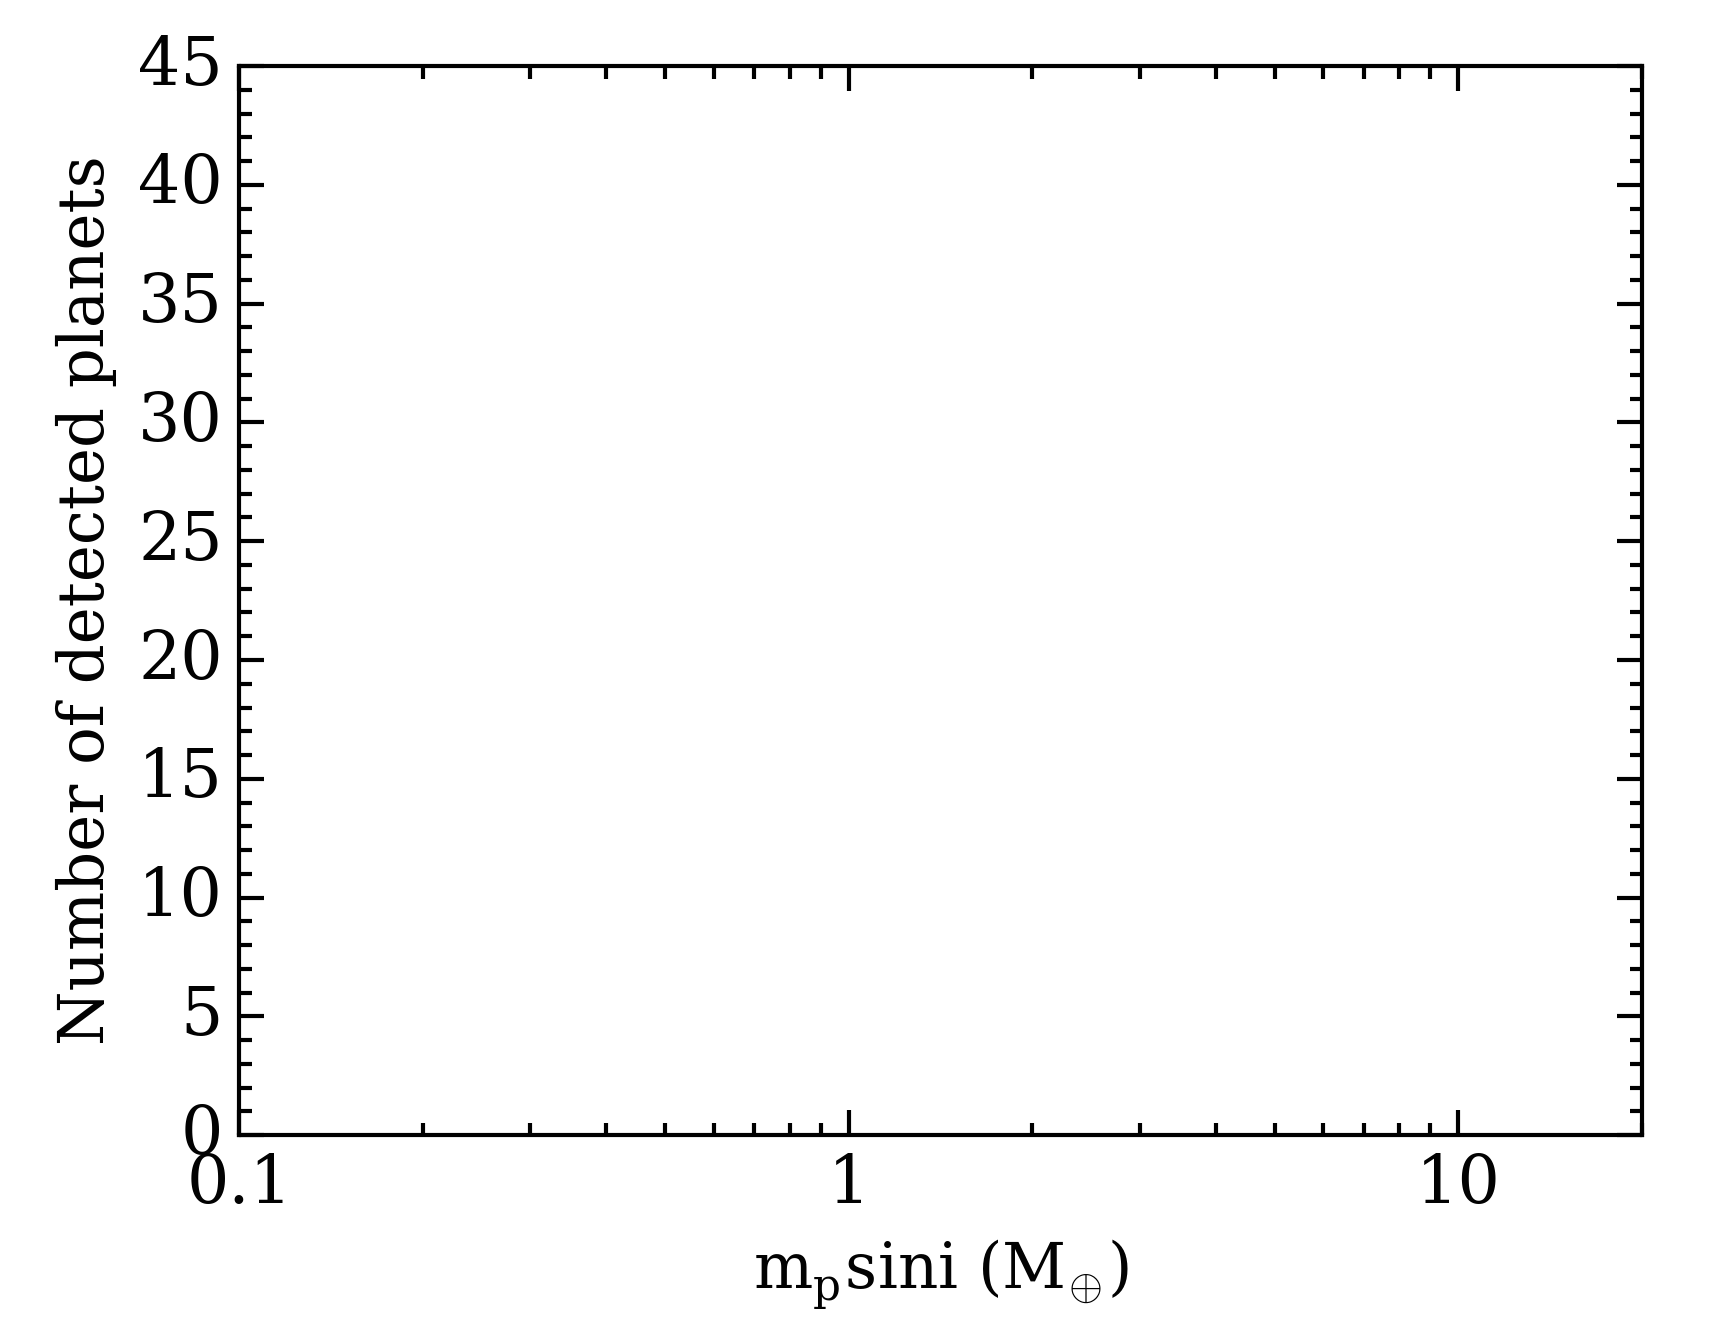
\includegraphics[width=0.6\hsize]{figures/detectedpopulations_bkgd.png}%
  \hspace{-0.6\hsize}%
  \begin{ocg}{fig:1off}{fig:1off}{0}%
  \end{ocg}%
  \begin{ocg}{fig:1on}{fig:1on}{1}%
    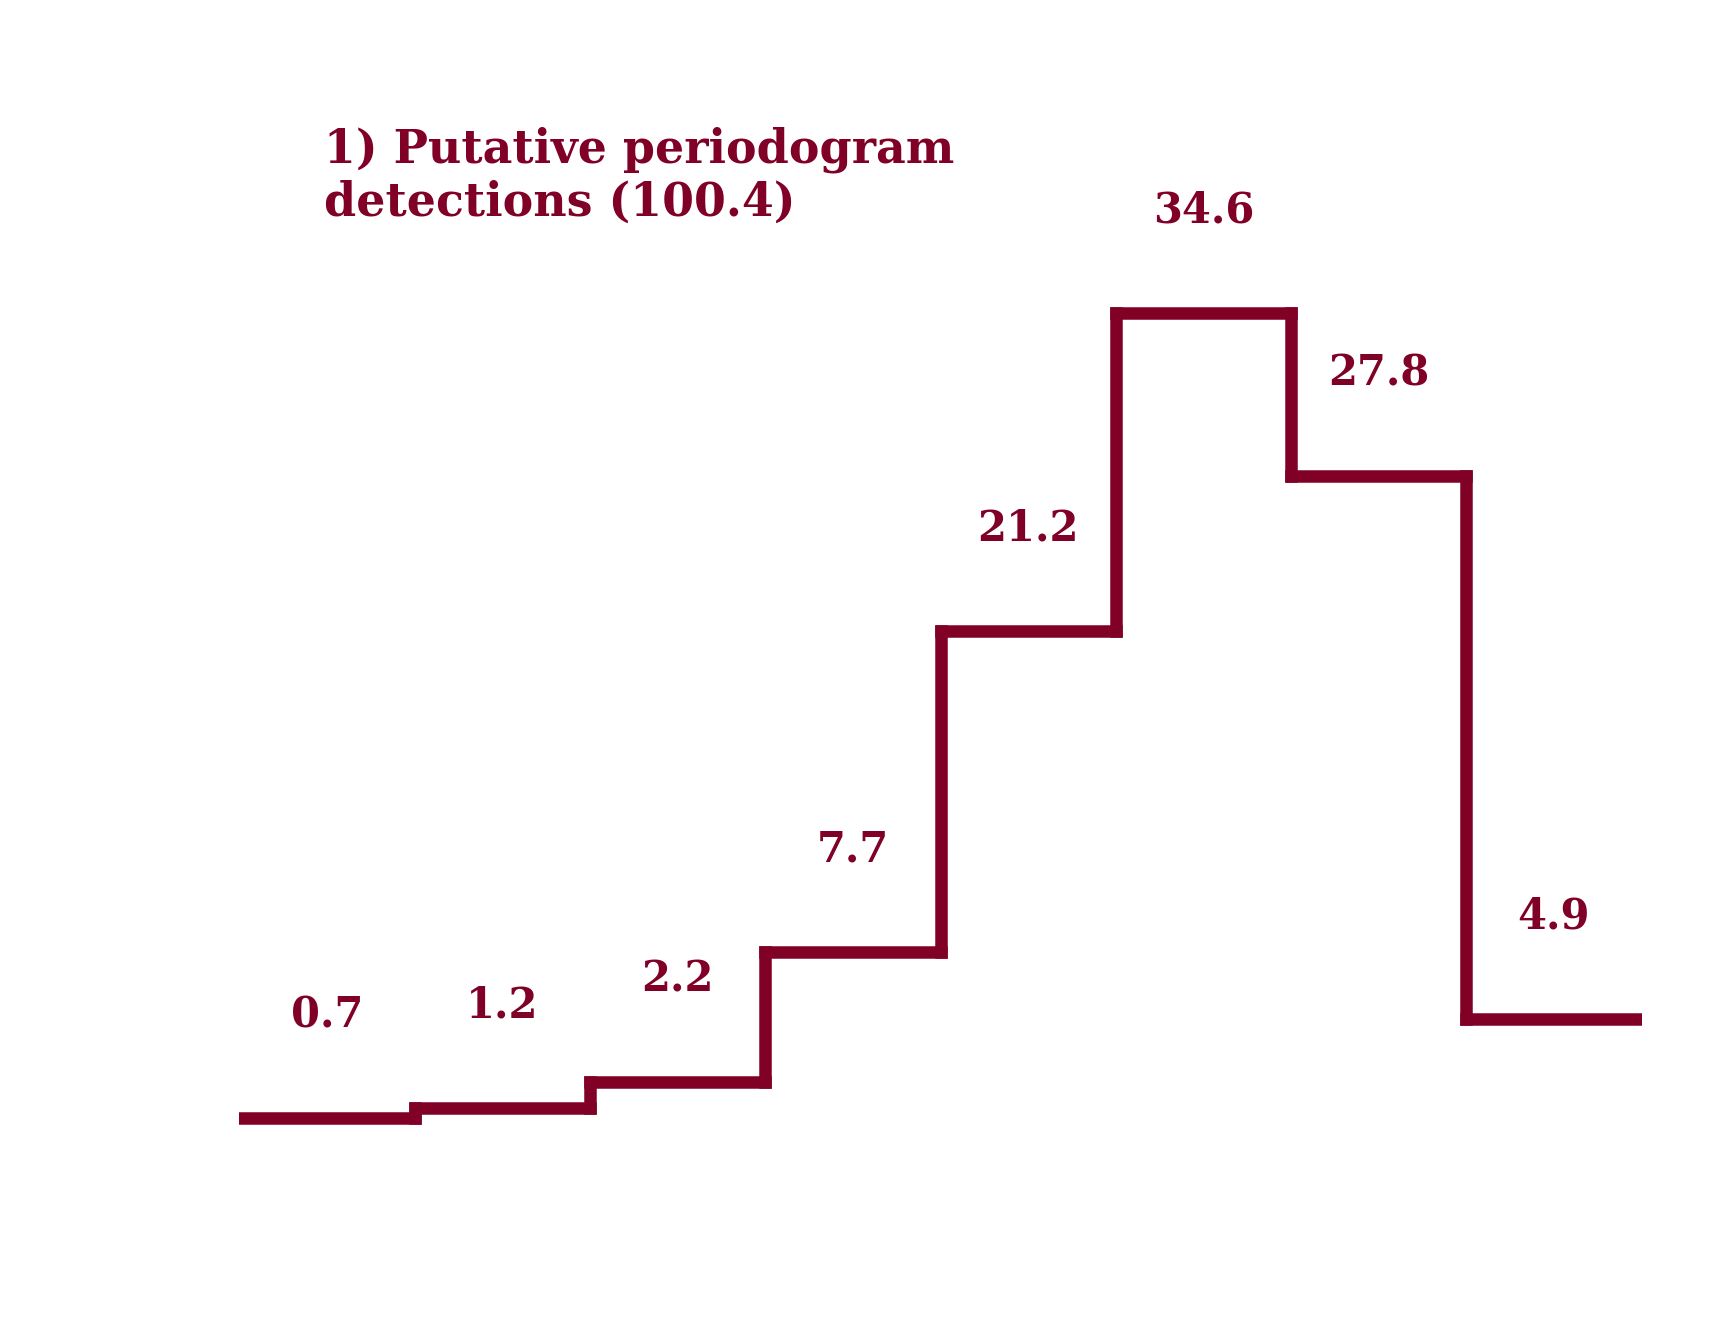
\includegraphics[width=0.6\hsize]{figures/detectedpopulations_1.png}%
  \end{ocg}
  \hspace{-0.6\hsize}%
  \begin{ocg}{fig:2off}{fig:2off}{0}%
  \end{ocg}%
  \begin{ocg}{fig:2on}{fig:2on}{1}%
    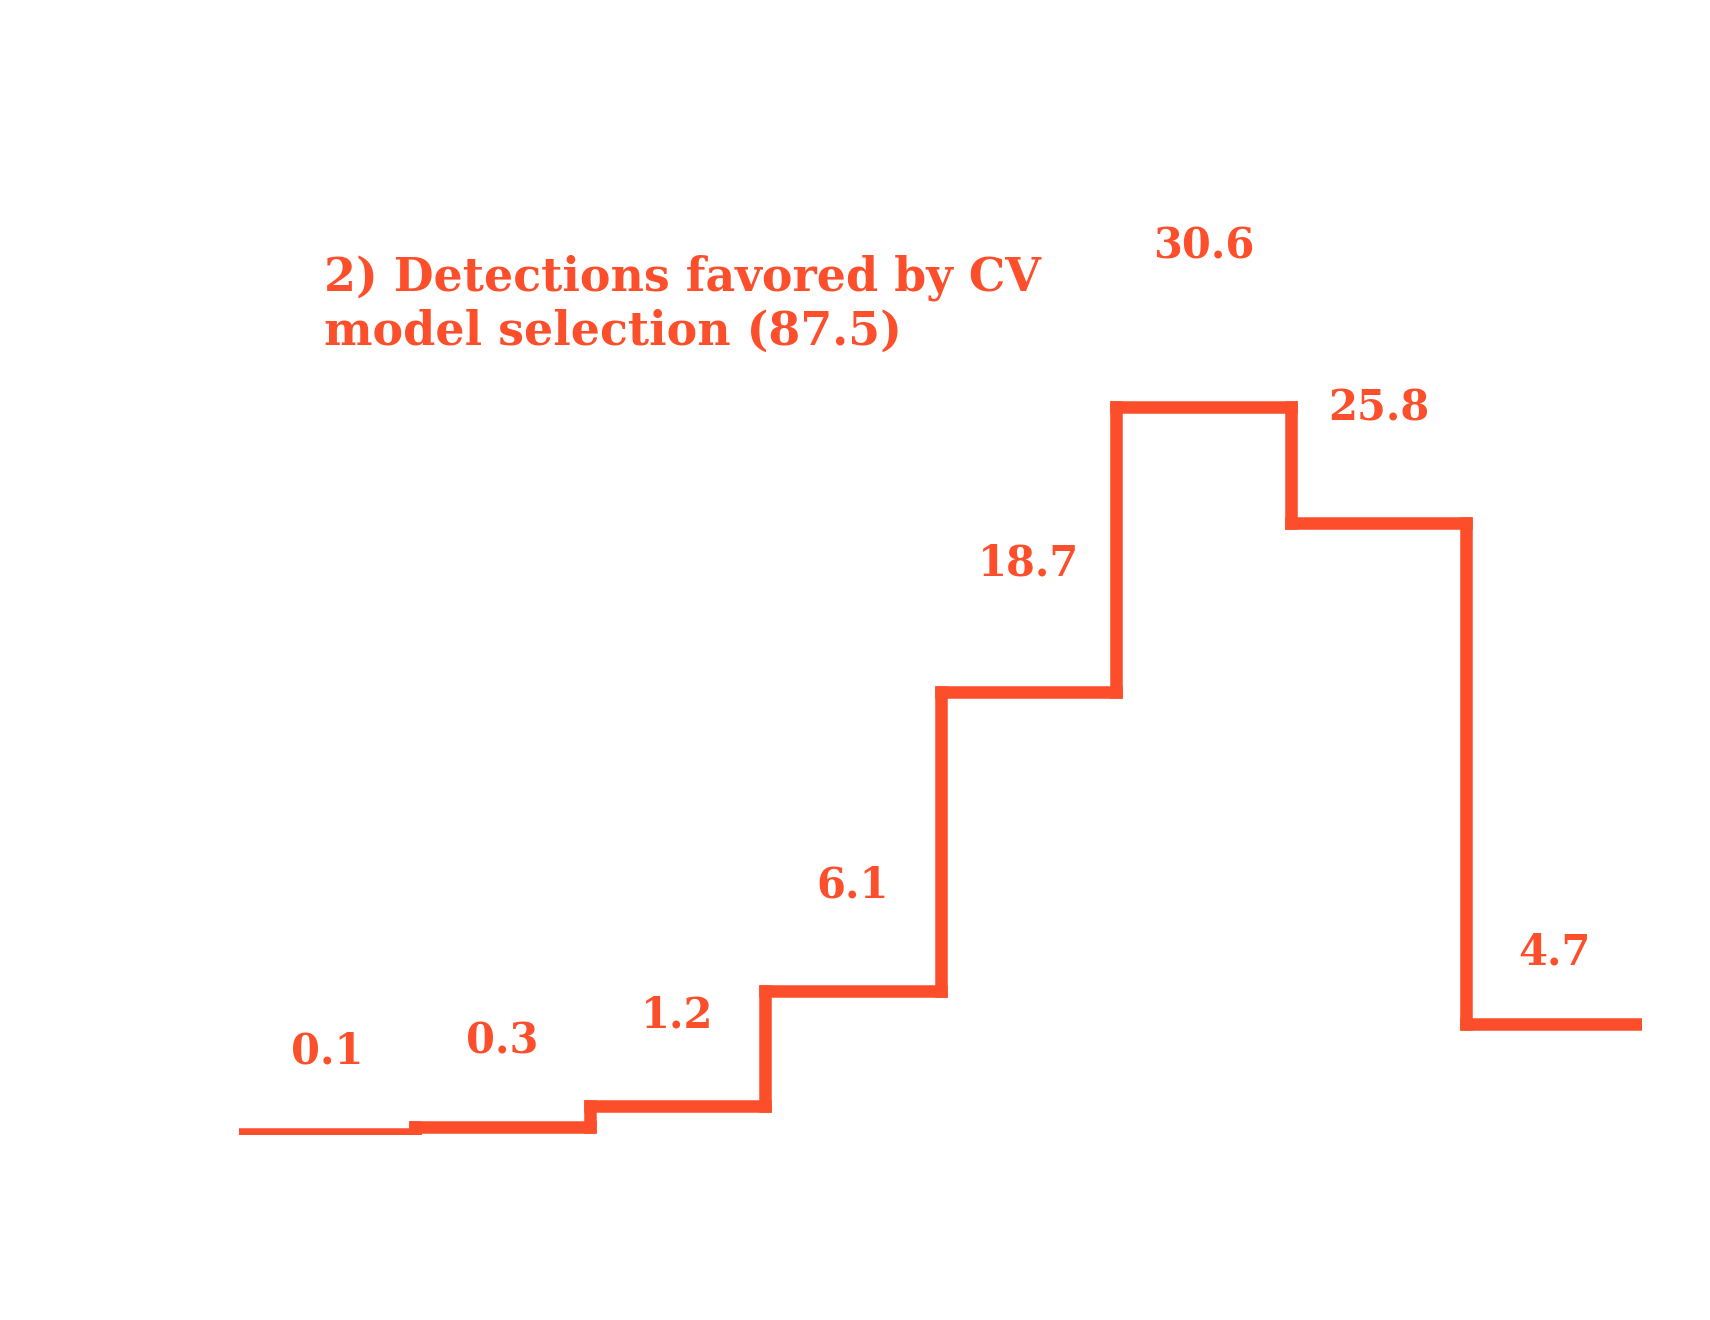
\includegraphics[width=0.6\hsize]{figures/detectedpopulations_2.png}%
  \end{ocg}
  \hspace{-0.6\hsize}%
  \begin{ocg}{fig:3off}{fig:3off}{0}%
  \end{ocg}%
  \begin{ocg}{fig:3on}{fig:3on}{1}%
    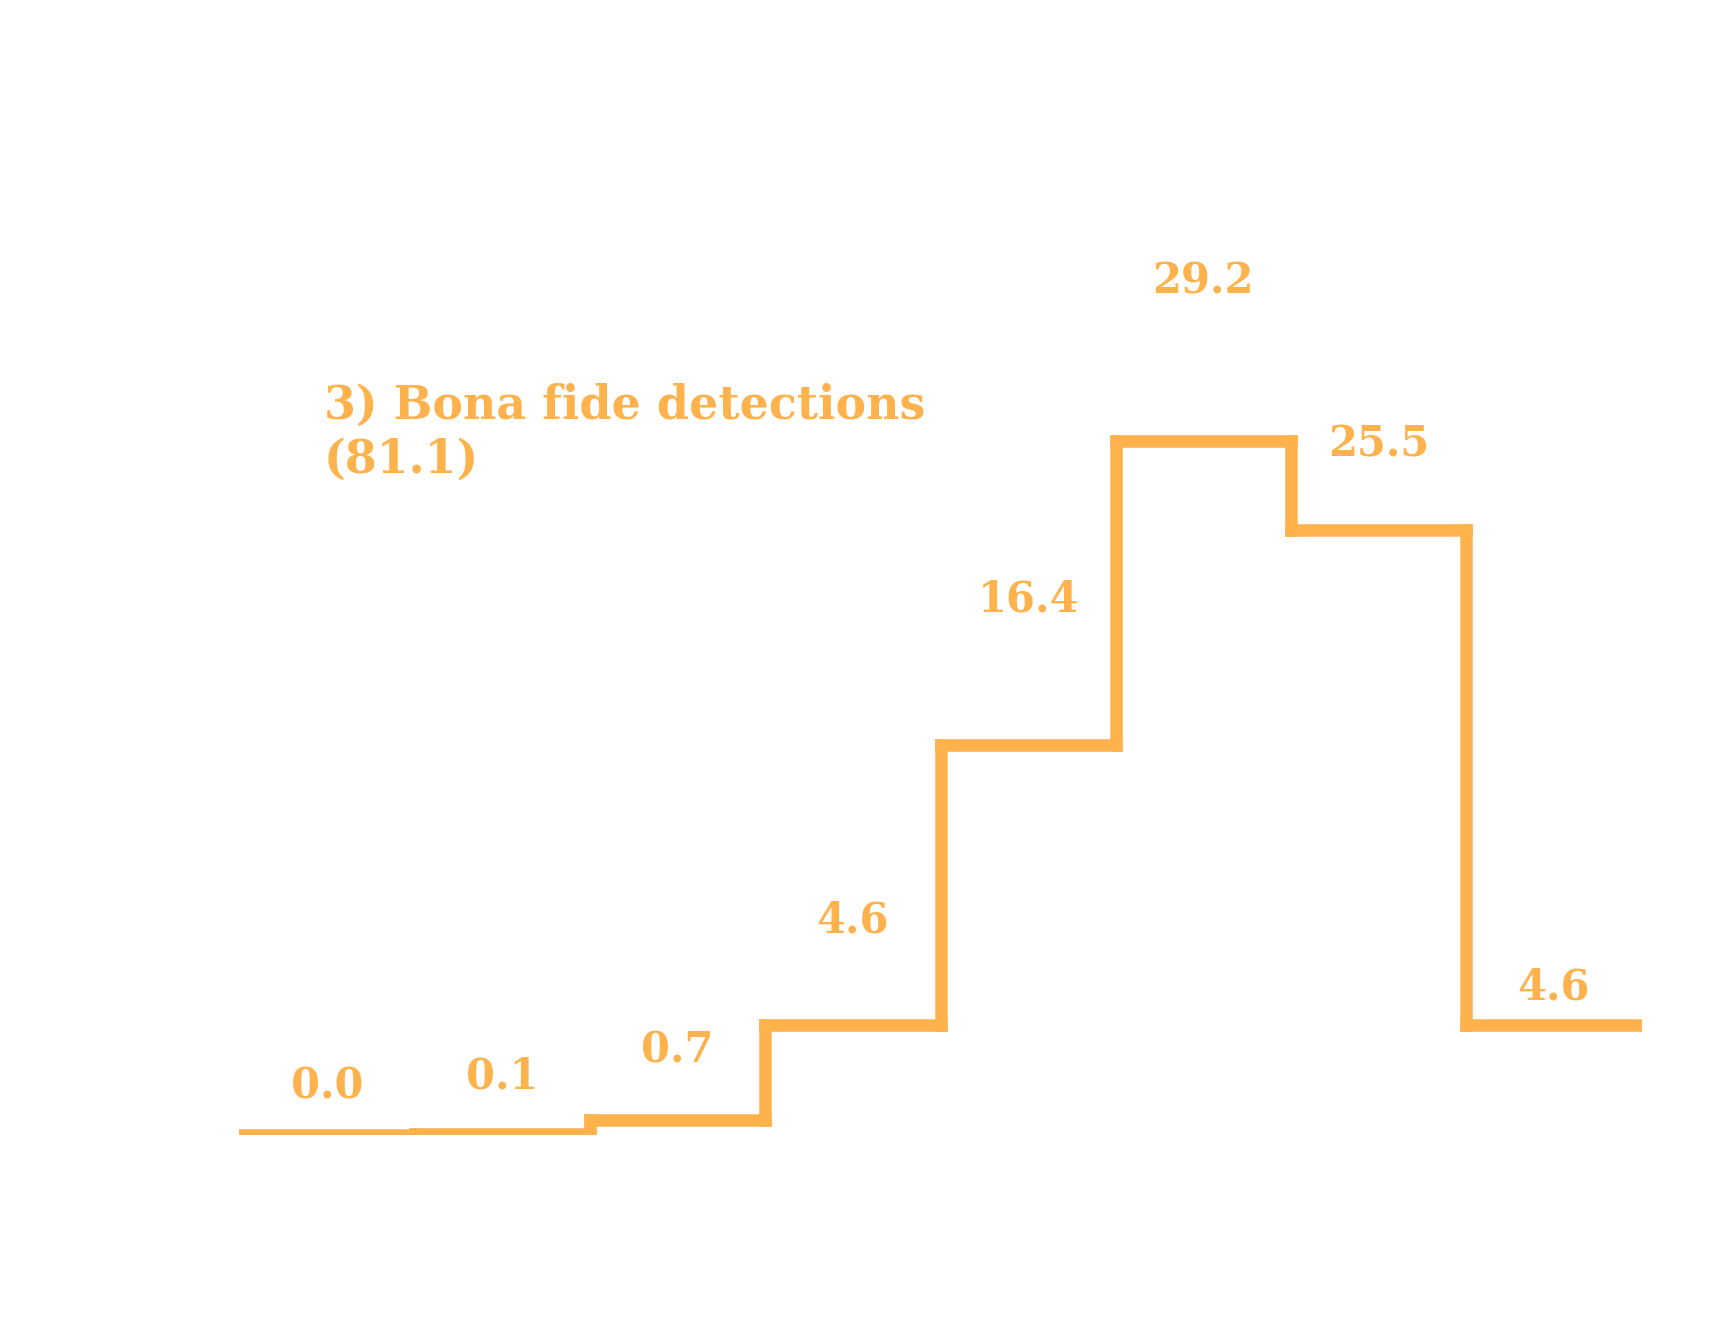
\includegraphics[width=0.6\hsize]{figures/detectedpopulations_3.png}%
  \end{ocg}
  \hspace{-0.6\hsize}%
  \caption[SPIRou planet yields versus \msini{} throughout the vetting process.]
      {\small The number of planets detected as a function of \msini{} after each of the three steps in
    our automated planet detection algorithm. The number of detected planets in each
    \msini{} bin is annotated above the bin to help quantify the decrease in planet detections
    following each step. The distribution of detected planet minimum masses
    following each step can be viewed independently for clarity
    (\ToggleLayer{fig:1off,fig:1on}{\protect\cdbox{1}},
    \ToggleLayer{fig:2off,fig:2on}{\protect\cdbox{2}},
    \ToggleLayer{fig:3off,fig:3on}{\protect\cdbox{3}}).}
    \label{BSfig:detections}
\end{figure}

It is clear from Fig.~\ref{BSfig:detections} that each step in our automated planet detection algorithm
reduces the number of detected planets somewhat.
In each \msini{} bin other than the most massive bin ($9.4 \leq m_p\sin{i}/\text{M}_{\oplus} \leq 20$),
our CV model selection technique rejects between $\sim 1-3$ planets or
$\sim 13$\% of all putative planet detections in the range of minimum planet masses considered. Similarly
our vetting procedure reduces the number of detected planets in each \msini{} bin by $\sim 1-2$ planets
for intermediate minimum masses; $0.7 \lesssim m_p\sin{i}/\text{M}_{\oplus} \lesssim 6$.
Our vetting procedure therefore does not reject a significant number of detected
planets at the lowest masses (\msini{} $\lesssim 0.7$ M$_{\oplus}$) nor at the highest
(\msini{} $\gtrsim 6$ M$_{\oplus}$). The former being the result of the small number of putative low mass planets
detected and the latter being due to the large RV semi-amplitude of the most massive planets thus resulting
in a typically large detection significance. Vetting rejects $\sim 7$\% of planet detections favored by
CV. Therefore $\sim 80$\% of putative planet detections from the periodogram analysis materialize
into bona fide planet detections.


\section{SLS-PS Sensitivity} \label{BSsect:sensitivity}
The detection sensitivity is defined as the recovery fraction of injected planets in our simulated SLS-PS.
Because we have a-priori knowledge of the injected planet population we can compute the detection sensitivity
for each star in our sample by simply dividing the number of detected planets by the number of injected
planets over any desired range of planet properties. We perform this calculation over the discretized
parameter space in $P$, \msini{} and in $S$, \msini{.}
Here $S=L_s / 4\pi a^2$ is the insolation received by the planet where $L_s$ is the stellar
luminosity\footnote{The stellar luminosity is computed from the evolutionary models of \cite{baraffe98} 
based on the stellar mass on the main sequence at 2 Gyrs.} and $a$ is the planet's semi-major axis. We 
focus on the
following ranges of parameter values which encompass the vast majority of the injected planet population:
$P \in [0.5,200]$ days, $S \in [0.01,100]$ S$_{\oplus}$, and \msini{} $\in [0.4,15]$ M$_{\oplus}$.  \\

We note that in this
study the recovery fraction is uniquely determined by the performance of our automated planet detection  
algorithm (see Sect.~\ref{BSsect:detection}). Conversely, the actual SLS-PS will have a much higher degree of
human intervention on the data analysis effort. This is afforded by the relatively small size of the RV
datasets compared to large surveys (e.g. Kepler and TESS)
which benefit greatly from automated detection algorithms. Therefore the detection sensitivity in the actual
SLS-PS may not correspond exactly to what is presented here although the automated algorithm used
in this study is designed to closely mimic the analysis that will be conducted on the actual SLS-PS data. \\

The detection sensitivity to planets varies from star-to-star due to their changing stellar
properties which can affect our ability to detect planets in radial velocity (e.g. apparent magnitude,
stellar mass, stellar rotation, etc).
Computing the detection sensitivity for each star individually is necessary for calculating planet
occurrence rates (see Sect.~\ref{BSsect:measurements}). To improve the detection statistics across the
full range of planetary parameters considered we augment the MC realizations for each star with an additional
set of planetary systems with logarithmic $P$, $S$, and \msini{} sampled uniformly rather than from the
planet occurrence rates. The individual detection sensitivity maps for each star can then be combined
to obtain the average sensitivity maps for the full
SLS-PS as a function of $P$, $S$ and \msini{} as shown in Fig.~\ref{BSfig:sensitivity}.
In this way we marginalize over the stellar properties of our sample stars including
the aforementioned parameters which are known to influence the detection sensitivity for each individual
star. Hence our sensitivity results might be scaled to various stellar samples provided that its global
properties are consistent with our current sample. In Fig.~\ref{BSfig:sensitivity}
the uncertainties in the detection sensitivity within each grid cell come from counting or Poisson
statistics and therefore benefit from a large number of simulated planetary systems. \\

\begin{figure*}
  \centering
  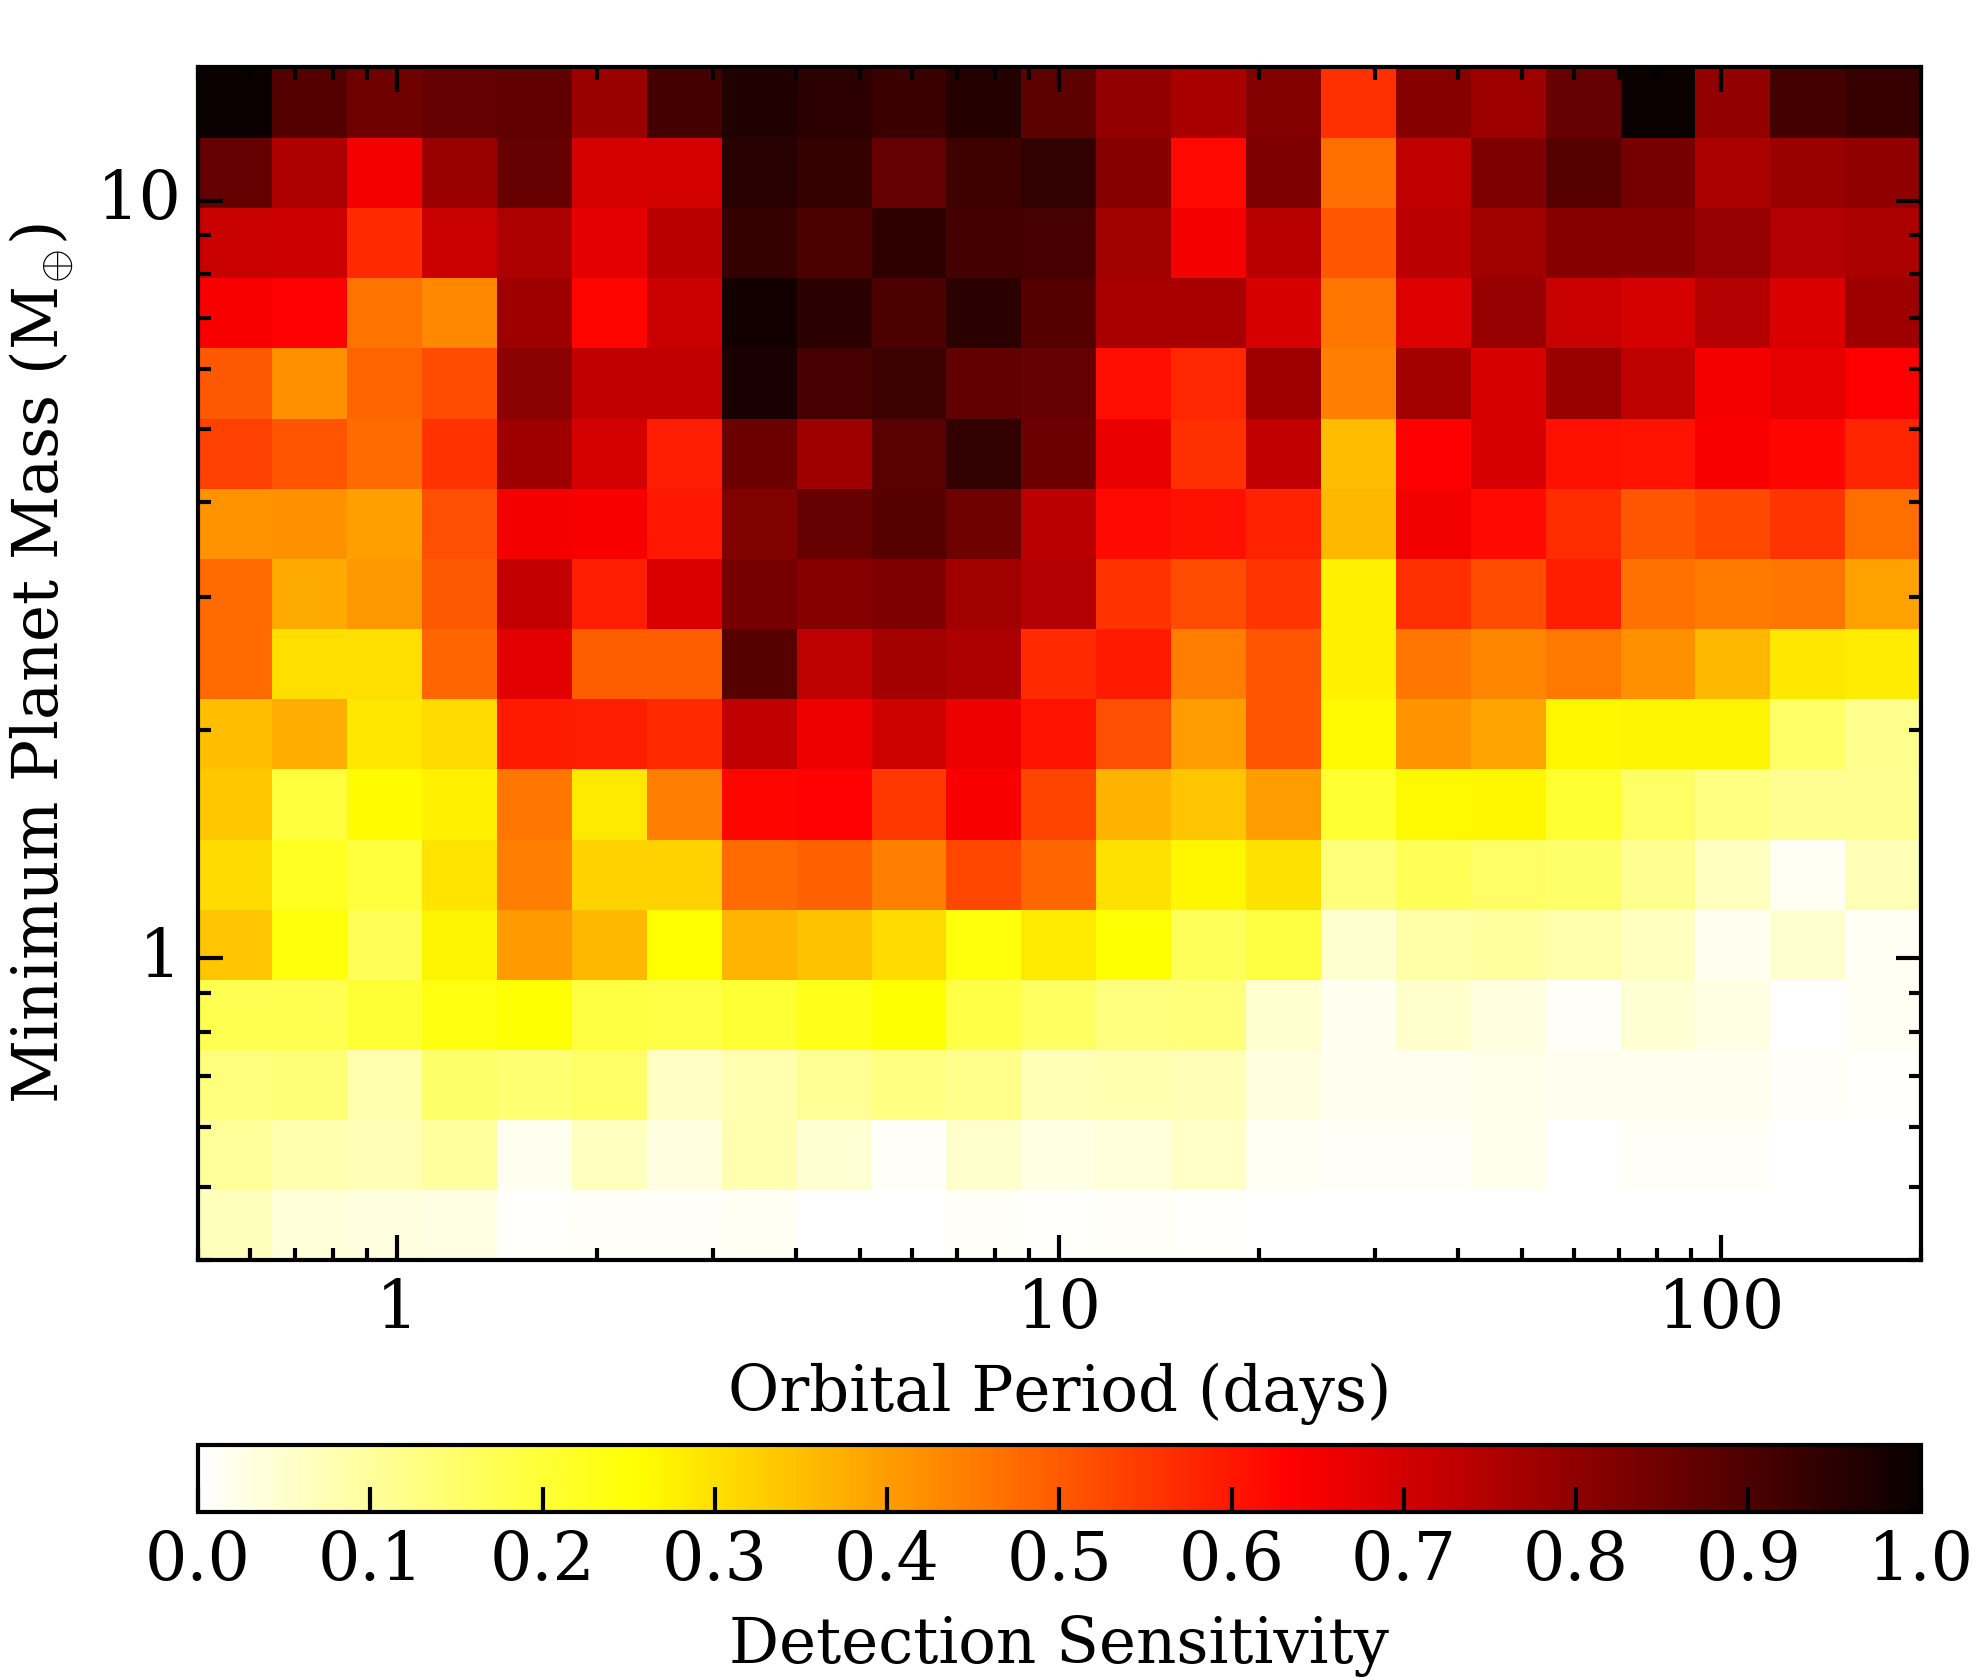
\includegraphics[width=0.5\hsize]{figures/sensPMpsini_bkgd_pickles_optimized100_final.png}%
  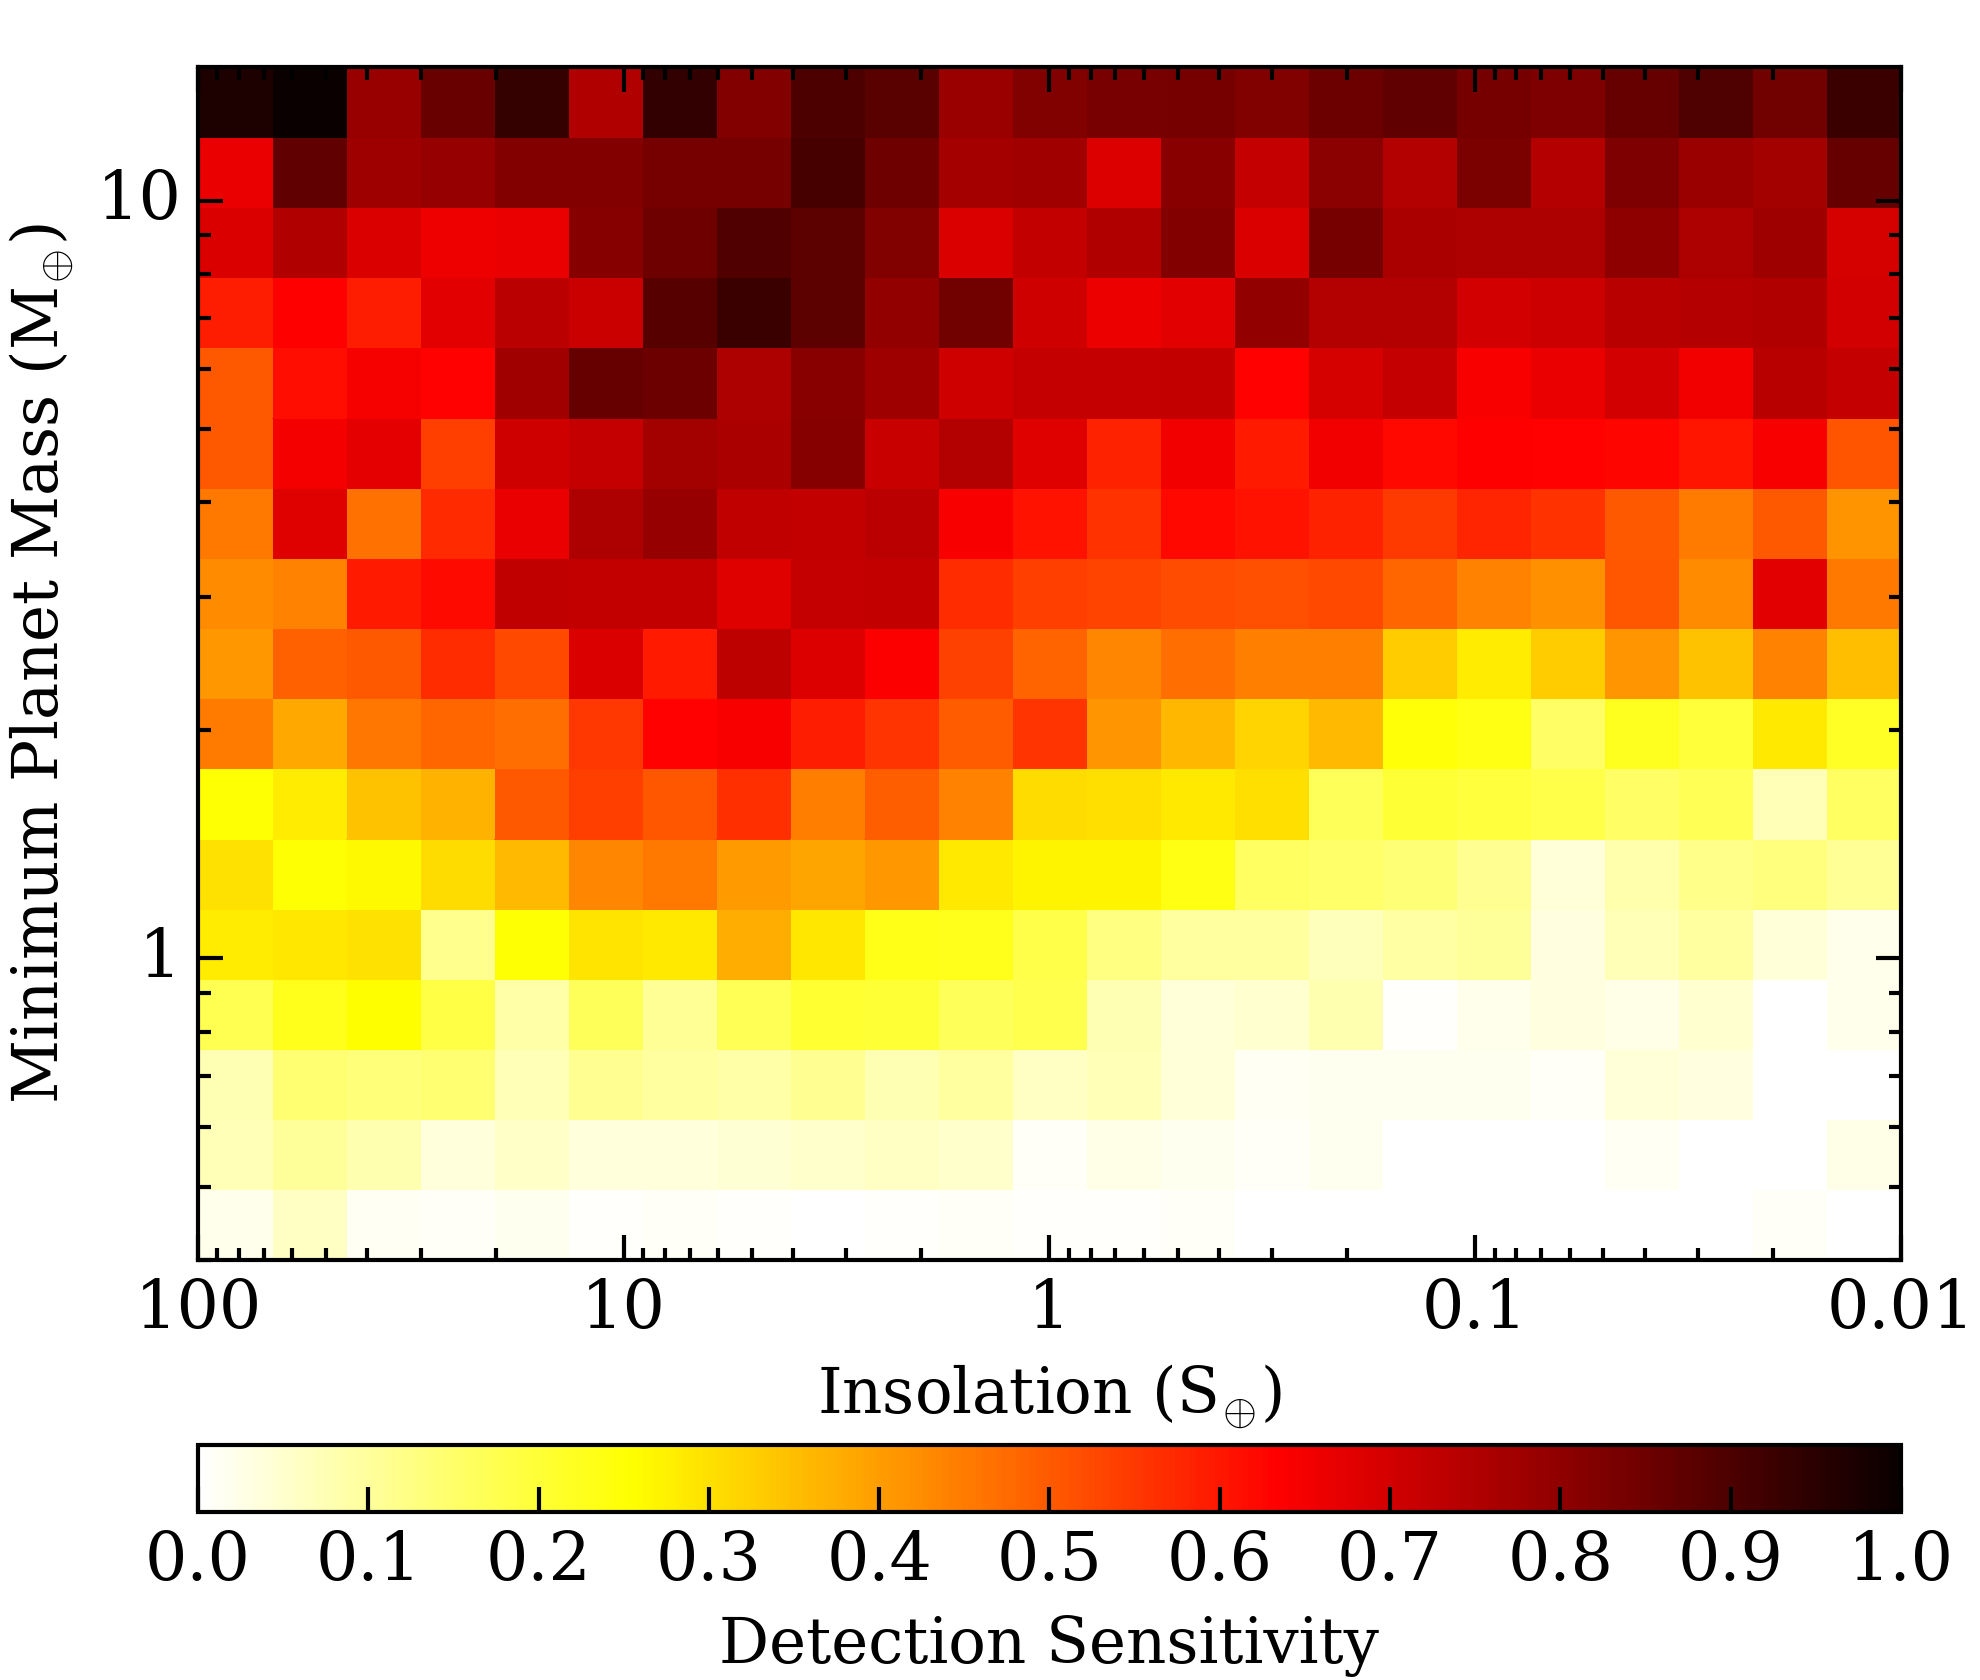
\includegraphics[width=0.5\hsize]{figures/sensFMpsini_bkgd_pickles_optimized100_final.png}%
  \hspace{-\hsize}%
  \begin{ocg}{fig:shadeoff}{fig:shadeoff}{0}%
  \end{ocg}%
  \begin{ocg}{fig:shadeon}{fig:shadeon}{1}%
    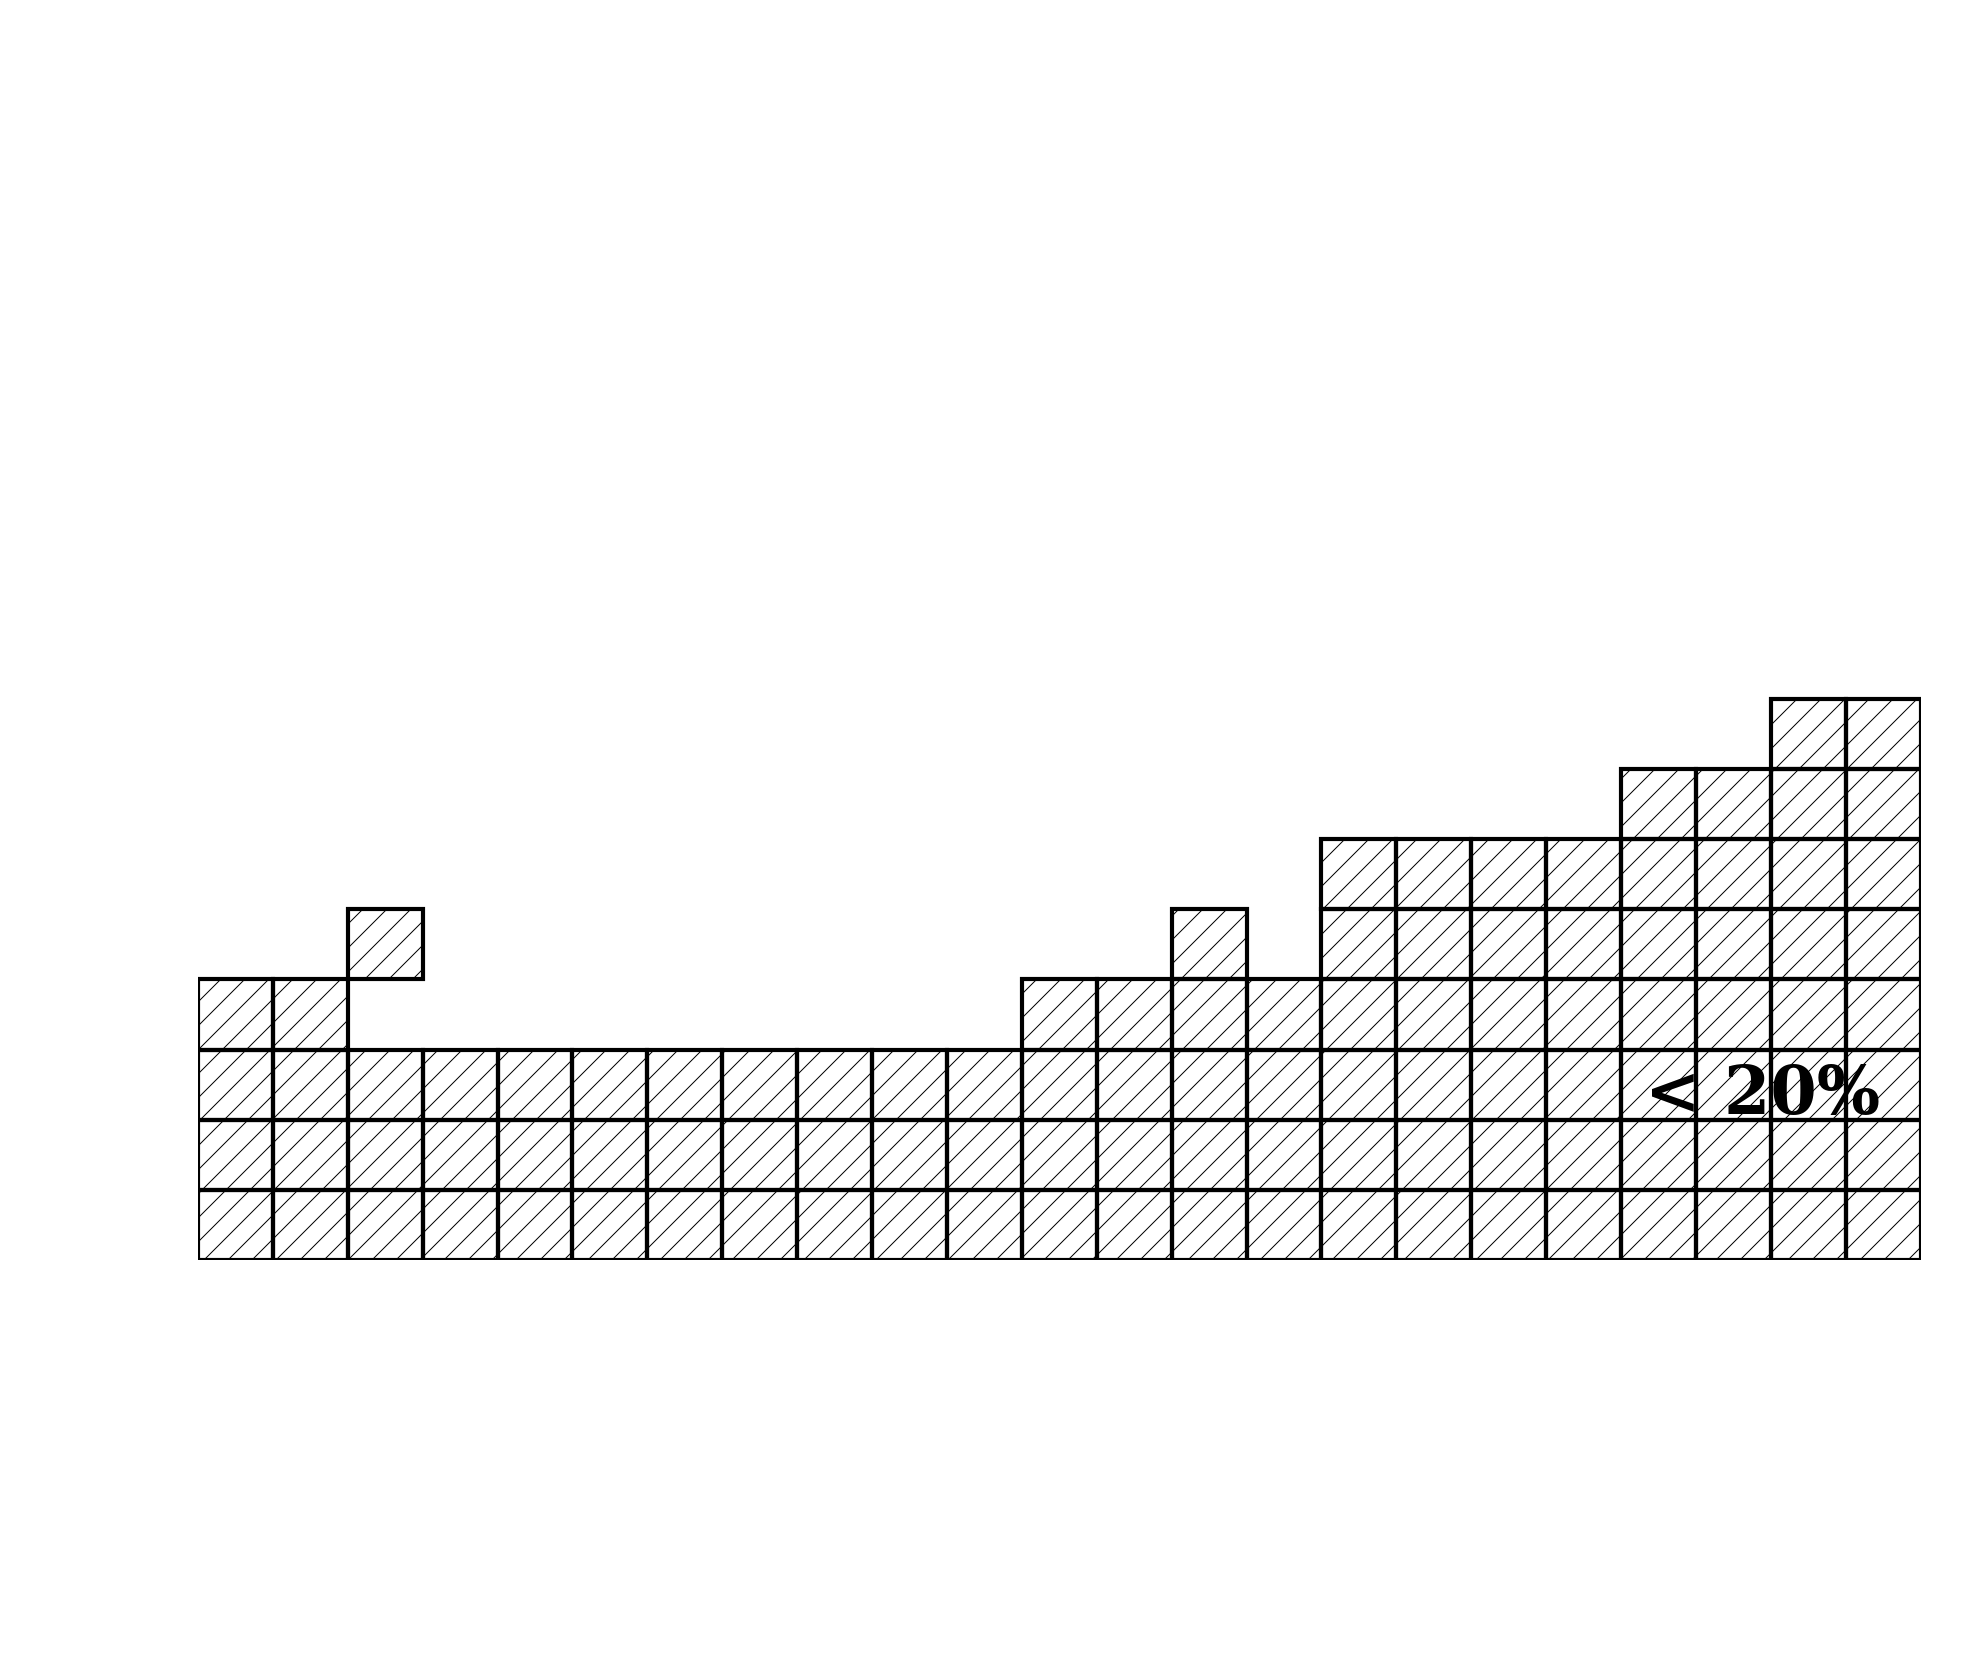
\includegraphics[width=0.5\hsize]{figures/sensPMpsini_shade_pickles_optimized100_final.png}%
    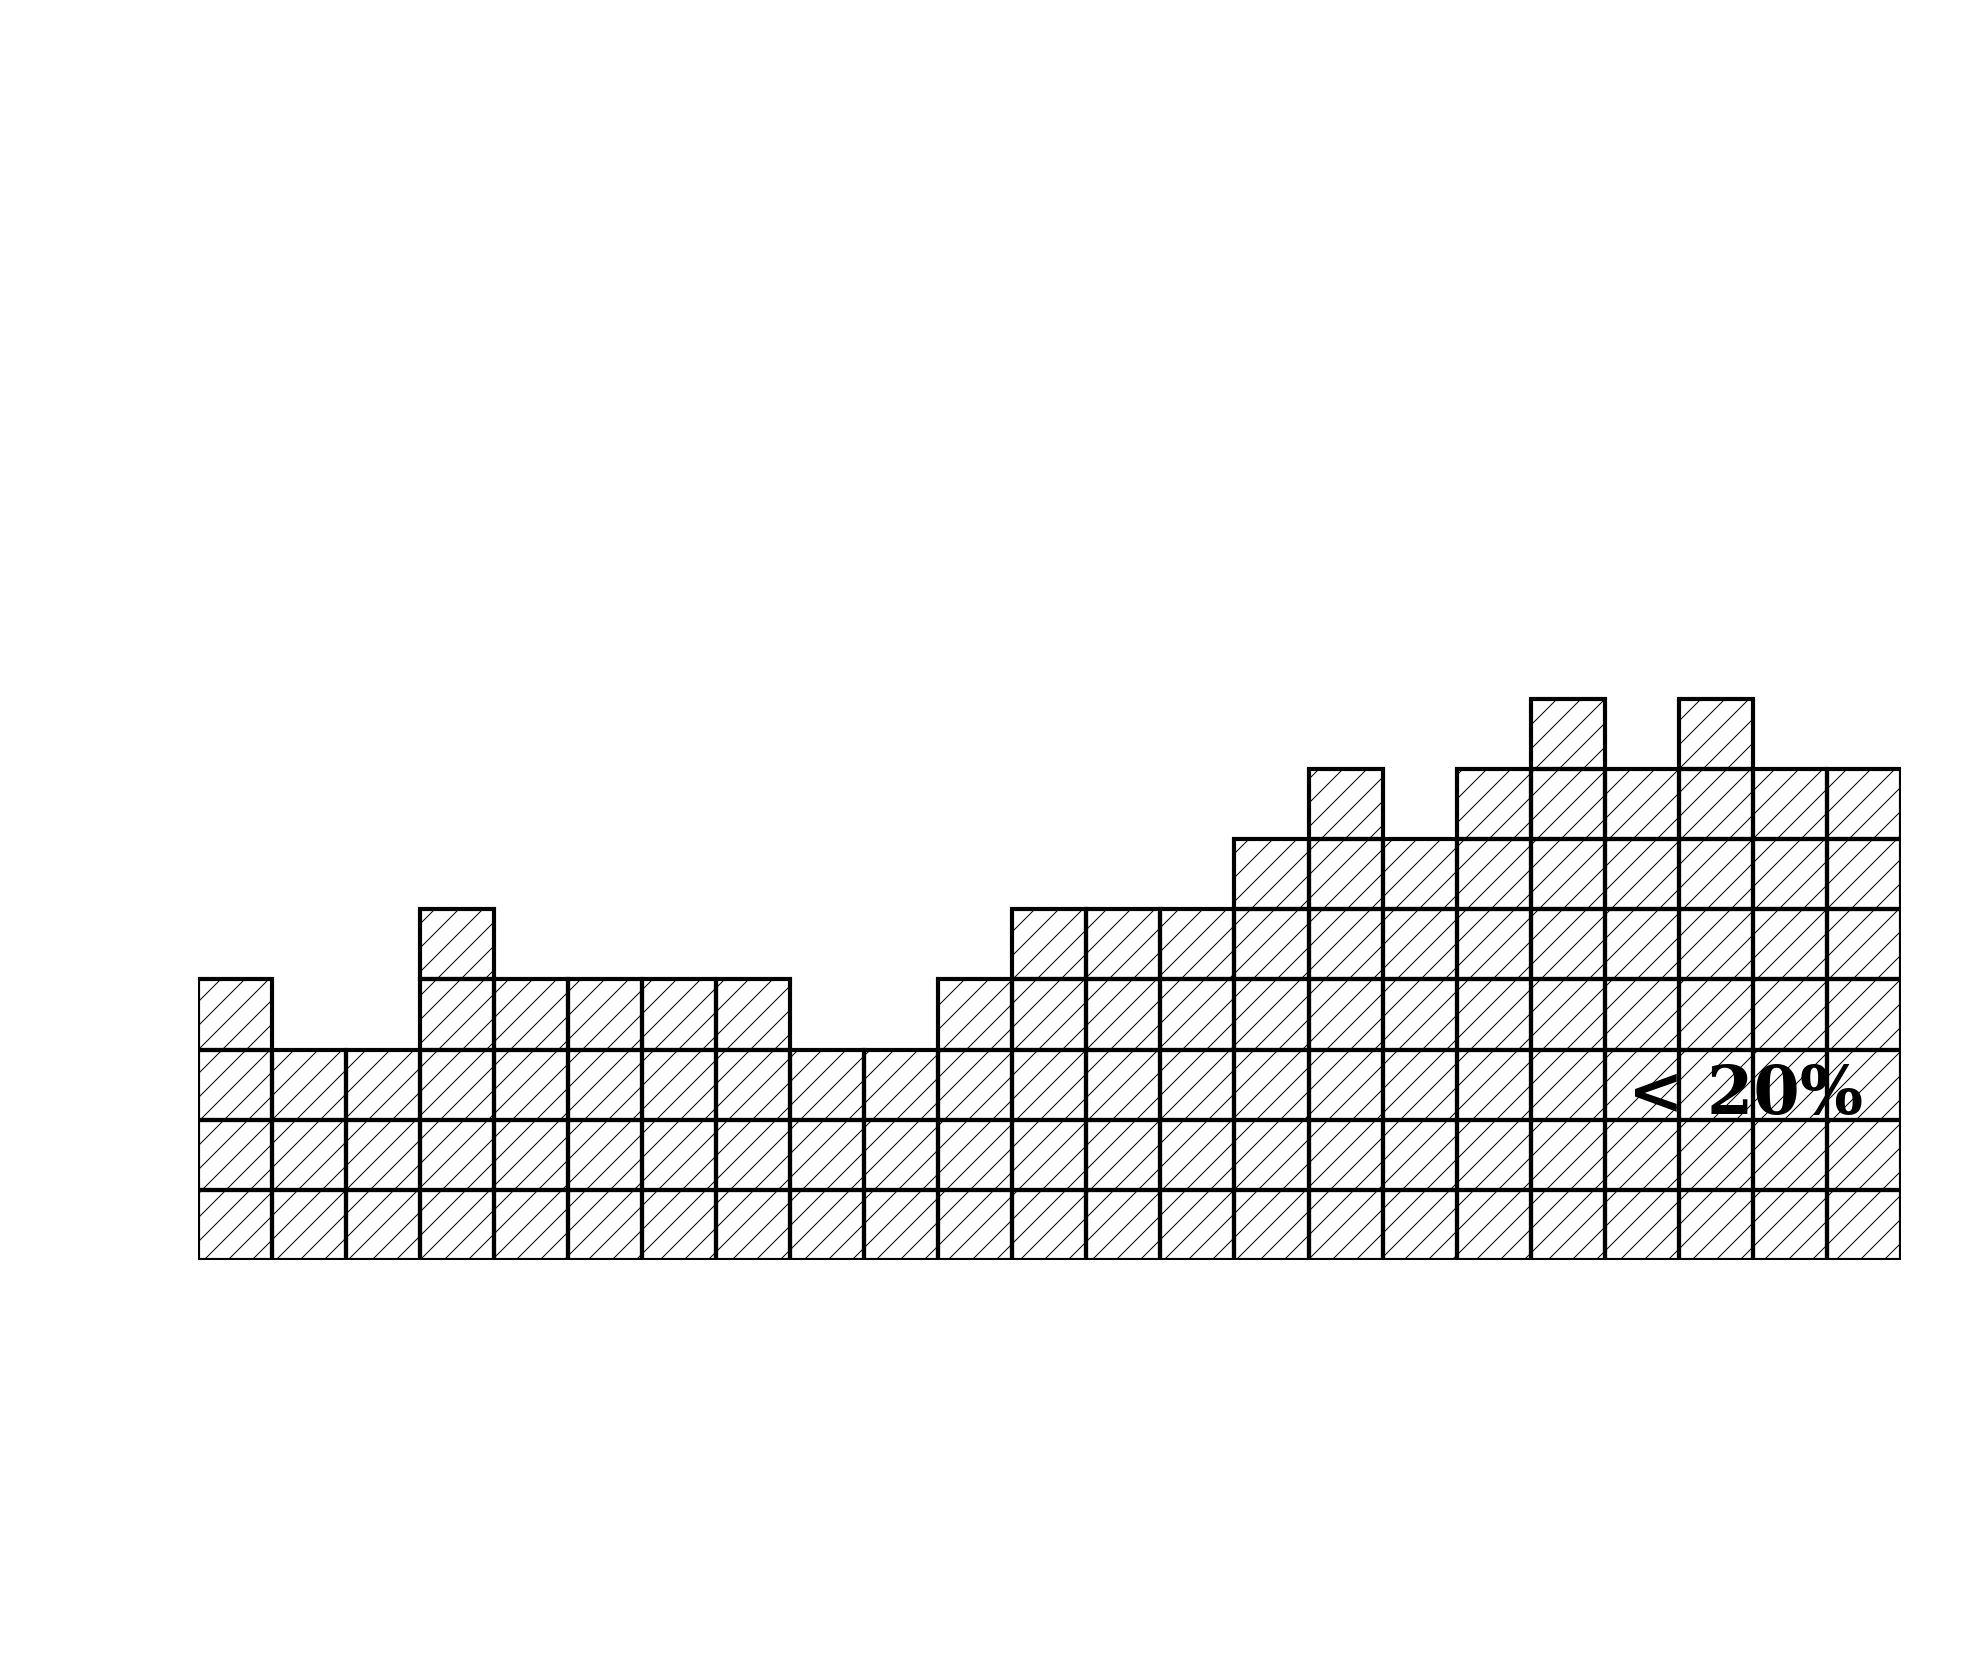
\includegraphics[width=0.5\hsize]{figures/sensFMpsini_shade_pickles_optimized100_final.png}%
  \end{ocg}
  \hspace{-\hsize}%
  \begin{ocg}{fig:Koff}{fig:Koff}{0}%
  \end{ocg}%
  \begin{ocg}{fig:Kon}{fig:Kon}{1}%
    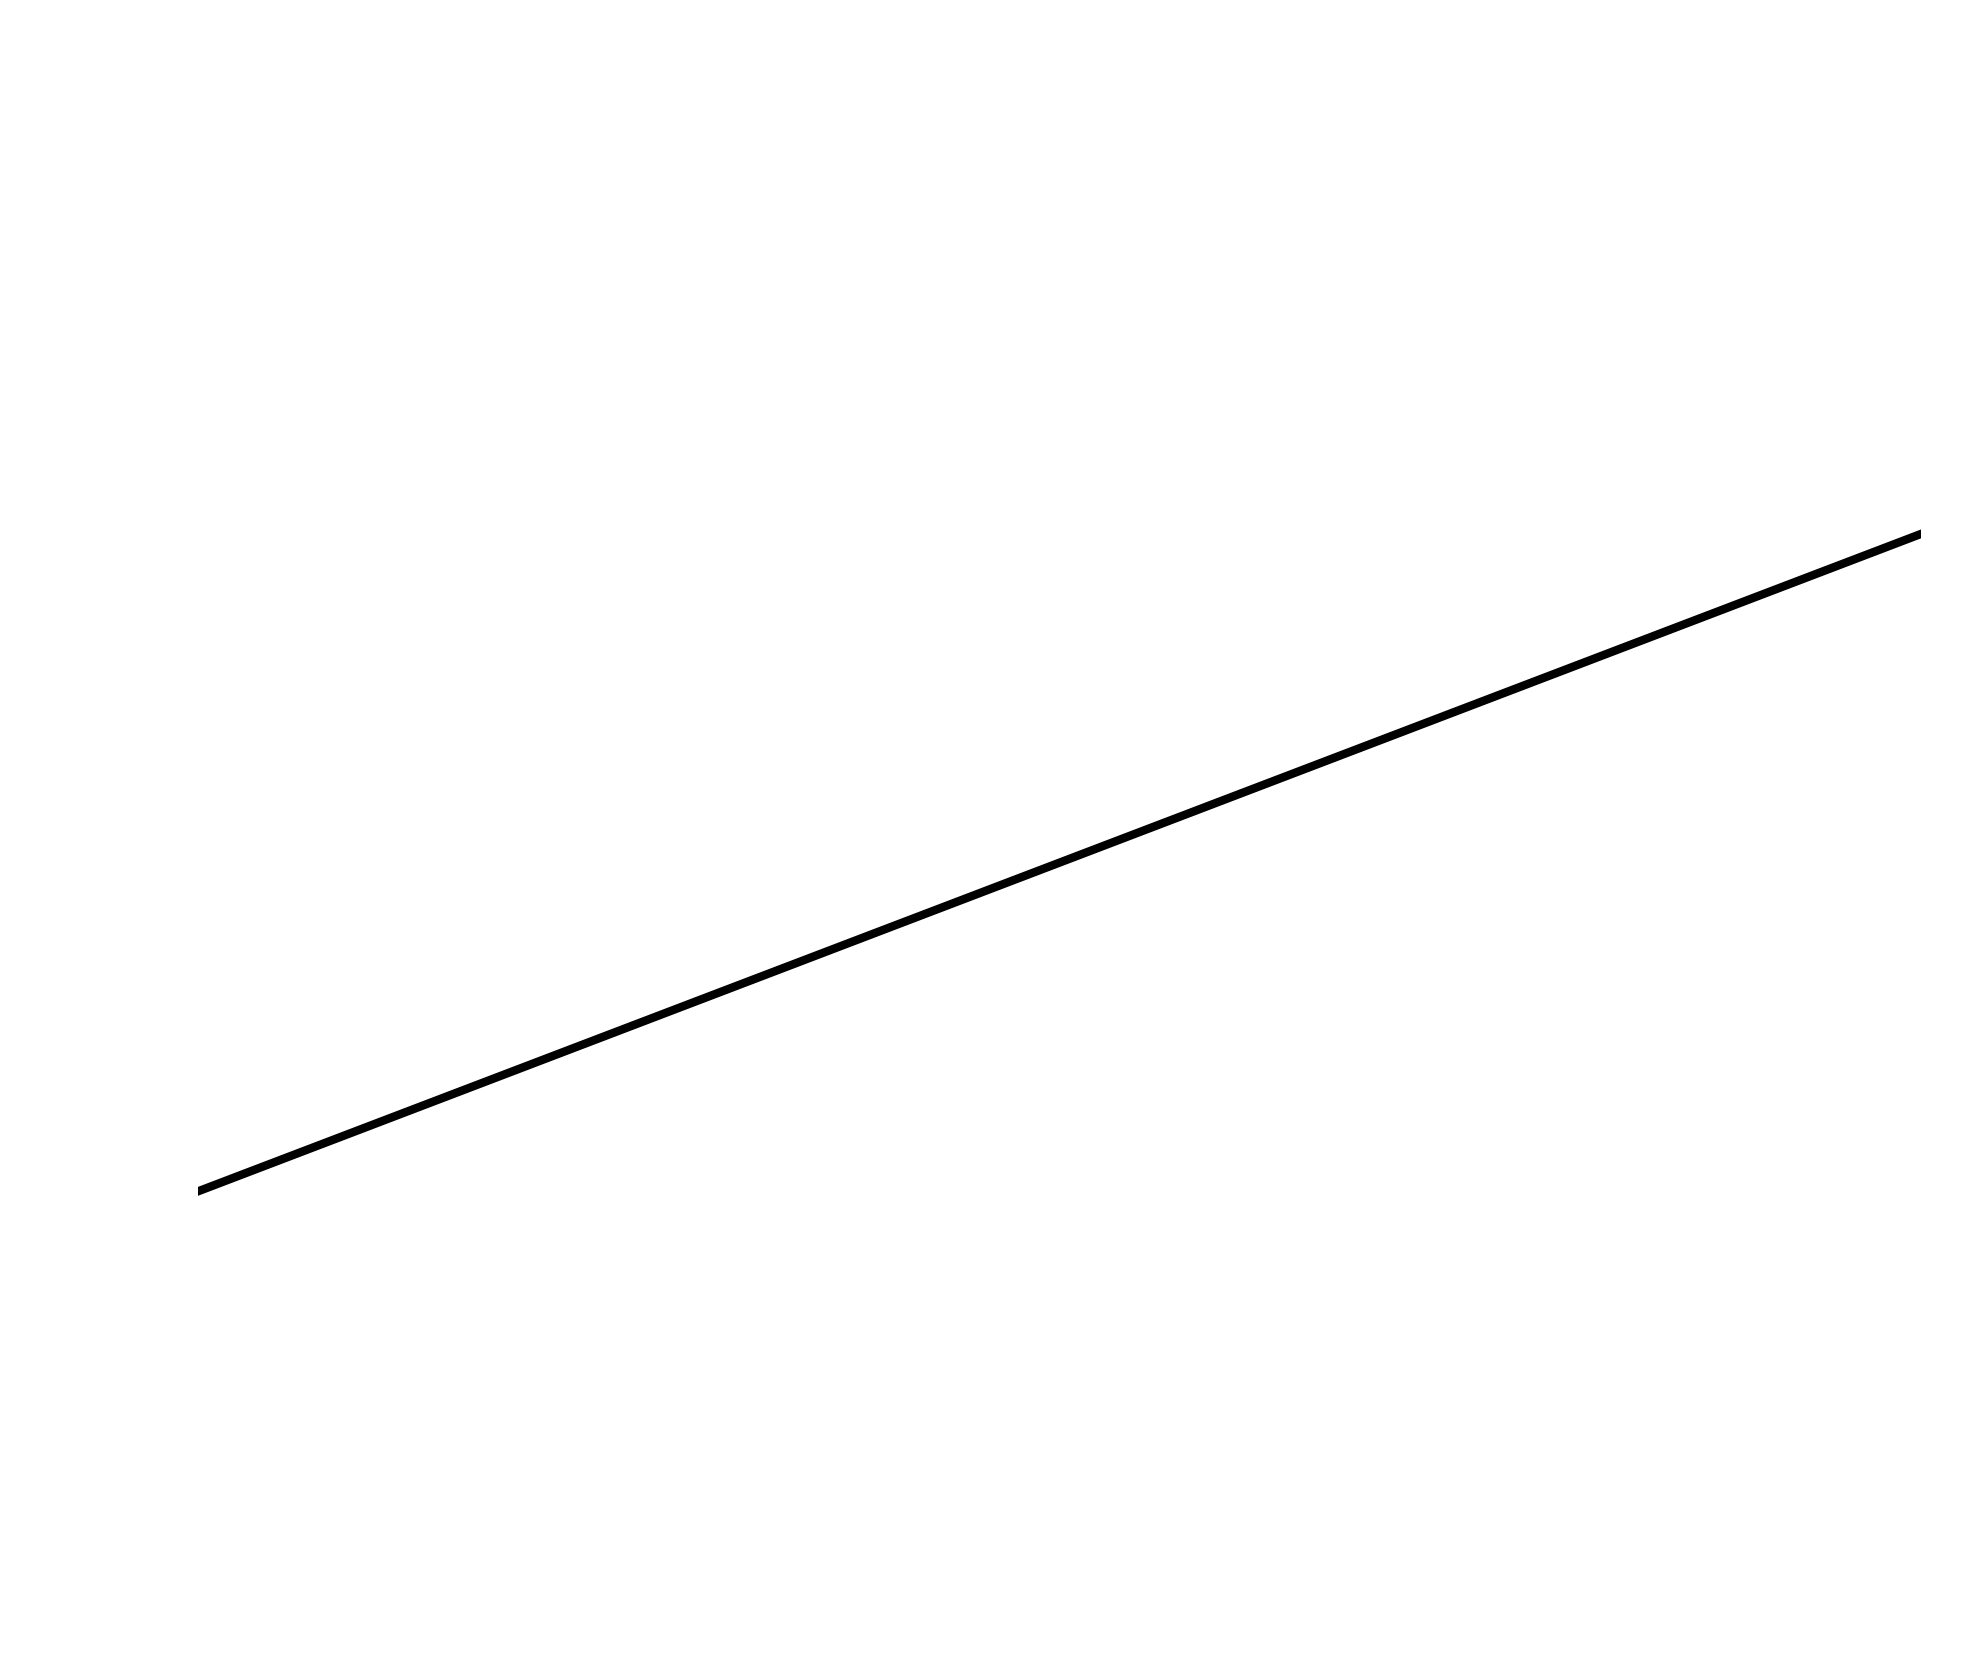
\includegraphics[width=0.5\hsize]{figures/sensPMpsini_Kline_pickles_optimized100_final.png}%
    \includegraphics[width=0.5\hsize]{figures/sensFMpsini_Kline_pickles_optimized100_final.png}%
  \end{ocg}
  \hspace{-\hsize}%
  \begin{ocg}{fig:HZoff}{fig:HZoff}{0}%
  \end{ocg}%
  \begin{ocg}{fig:HZon}{fig:HZon}{1}%
    \includegraphics[width=0.5\hsize]{figures/yieldPMpsini_HZ.png}%
    \includegraphics[width=0.5\hsize]{figures/yieldFMpsini_HZ.png}%
  \end{ocg}
  \hspace{-\hsize}%
  \caption[Detection sensitivity maps in the SLS-PS.]
      {\small Binned maps of the detection sensitivity of the full SPIRou input catalog derived using our
    automated planet detection algorithm as a function of minimum planet mass and orbital period 
    (\emph{left}) or insolation (\emph{right}). The \emph{dashed vertical lines} in the
    insolation panel indicate the approximate `water-loss' and `maximum-greenhouse' insolation
    limits of the \ToggleLayer{fig:HZon,fig:HZoff}{\protect\cdbox{HZ}} from \cite{kopparapu13}.
    The \emph{dashed-dotted vertical lines}
    indicate the more conservative `recent-Venus' and `early-Mars' HZ limits \citep{kopparapu13}
    \ToggleLayer{fig:shadeon,fig:shadeoff}{\protect\cdbox{\emph{Shaded}}} bins highlight
    regions of the parameter space wherein our detection sensitivity is $<20$\%. The
    \ToggleLayer{fig:Kon,fig:Koff}{\protect\cdbox{\emph{solid lines}}} highlight the curve with $K=1$
    \mps{} for a star with mass equal to our sample's median stellar mass of 0.25 M$_{\odot}$.}
  \label{BSfig:sensitivity}
\end{figure*}


Given the binning in Fig.~\ref{BSfig:sensitivity}, nowhere do we achieve a 100\%
detection sensitivity. This is true even for the most massive close-in planets whose RV
semi-amplitudes are typically much greater than the characteristic RV measurement uncertainty so
long as the system is not orientated close to face-on (i.e. $\sin{i} \sim 0^{\circ}$). The geometric effect
as well as potential aliasing of periodic signals arising from stellar rotation or the window
function, also prevent the detection of certain types of planets. For example, in Fig.~\ref{BSfig:protcdf}
we see that in our stellar sample there is a dearth of \prot{} $\sim 3-10$ days. Thus
we run into minimal aliasing from \prot{} at those orbital periods and achieve an increased detection
sensitivity relative to planets with equivalent \msini{} but with smaller $P$
(\emph{left panel} Fig.~\ref{BSfig:sensitivity}). \\

Similarly we can see a steep decrease in detection sensitivity at periods of $\sim 30$ days. Recall that
in our window functions we are restricted by the telescope's observing schedule to only observe outside
of dark-time whose cycle follows the lunar cycle with a cadence of  $\sim 30$ days.
Consequently the origin of the
decrease in detection sensitivity at $\sim 30$ days can be traced back to aliasing from our time
sampling at that period; an unfortunate circumstance as the range of orbital periods corresponding to the
HZ around M2-4 dwarfs, spans 30 days.  \\

Due to the
aforementioned aliasing effects from stellar rotation and our window functions, the SPIRou detection
sensitivity is maximized for the most massive planets with $3 \lesssim P \lesssim 10$ days. 
Another pertinent effect at orbital periods close to one day is the potential for signal aliasing due to the
Earth's rotation. This---in part---is responsible for the low detection sensitivity at orbital periods close
to a day in Fig.~\ref{BSfig:sensitivity}; another unfortunate circumstance given the general interest in
quantifying the occurrence rate of close-in planets \citep{mulders15}. \\

The average detection sensitivity across the full range of $P$ and
\msini{} in Fig.~\ref{BSfig:sensitivity} is $44.8 \pm 0.5$\%.
This average detection sensitivity is sufficiently high such that the
resulting planet detections from the SLS-PS will be able to place strong constraints on the cumulative
occurrence rate of planets around SPIRou stars (see Sect.~\ref{BSsect:measurements}). \\

When considering the detection sensitivity as a function of insolation, we see the same
qualitative structure as is seen as a function of orbital period (\emph{right panel}
Fig.~\ref{BSfig:sensitivity}). For example, the increased
sensitivity between $\sim 3-10$ days has a broad manifestation at $S \in [1,10]$ S$_{\oplus}$.
Similarly, in both cases it is unsurprising to see that the detection sensitivity increases
towards more massive planets. In both cases the SPIRou
detection sensitivity reaches its lowest values for the least massive planets on wide-orbits.
Notably, we achieve a detection sensitivity of $\lesssim 20$\% for all planets with
\msini{} $\lesssim 1$ M$_{\oplus}$ thus making it difficult to detect Earth-mass planets and
smaller in the SLS-PS. The average detection sensitivity across the full range of $S$ and
\msini{} considered here is $47.6 \pm 0.5$\%.


\subsection{Detection Sensitivity to HZ Planets}
It is also important to consider our detection sensitivity to HZ planets as these targets are often
flagged for various observational follow-up campaigns. In this study we adopt the `water-loss' and
`maximum-greenhouse' definitions
as our fiducial HZ limits from \cite{kopparapu13} which are derived from a 1D radiative-convective
climate model in the absence of clouds. Following \cite{kasting93}, the inner edge of the HZ is defined
by the `water-loss' limit which arises from the photolysis of water in the upper atmosphere and subsequent
hydrogen escape. The outer edge of the HZ is determined by the `maximum-greenhouse' limit wherein an
increase in atmospheric CO$_2$ levels will result in a net cooling as the increased albedo from Rayleigh
scattering begins to dominate over the increasing greenhouse effect. The insolation levels 
approximately corresponding to our adopted HZ definition are $S \in [0.22,0.90]$ S$_{\oplus}$ for our
stellar sample. For comparison we
also consider the more conservative ($S \in [0.20,1.48]$ S$_{\oplus}$; \citealt{kopparapu13})
`recent-Venus' and `early-Mars' HZ limits which assume that both Venus and Mars were habitable early-on
in the lifetime of the Solar System. \\

From the fiducial definition of the HZ we find an average
detection sensitivity to HZ planets of $47.3 \pm 1.0$\% which is consistent with the average
detection sensitivity over the full $S$,\msini{} grid in the right panel
of Fig.~\ref{BSfig:sensitivity}
($46.2 \pm 0.5$\%). Adopting the more generous HZ limits, we find a comparable average
detection sensitivity of $48.7 \pm 0.9$\%.
However, the average detection sensitivity to Earth-like planets ($m_p \in [1,5]$ M$_{\oplus}$) in the HZ
is significantly reduced to $36.7 \pm 1.2$\%. Here we have defined Earth-like planets in terms of their
absolute mass where the mass upper limit is approximately equal to 
the planet mass obtained when evaluating the mean mass-radius relation (Eq.~\ref{BSeq:mr}) at the
proposed maximum radius of a rocky planet; $\sim 1.5-1.8$ R$_{\oplus}$ \citep{weiss14, rogers15, fulton17}.

\section{SLS-PS Predicted Yield} \label{BSsect:yield}
For each of the 100 stars in the SPIRou input catalog,
we can compute the number of planets detected as a function of $P$, $S$,
and \msini{} given the input occurrence rates and calculations of each star's detection sensitivity.
Here we must correct the reduced injected cumulative planet occurrence rate of 2.4 planets per star
over our grid of $P \in [0.5,200]$ days and \msini{} $\in [0.4,15]$ M$_{\oplus}$ to be equal to the
intended 2.5 planets per star over the \cite{dressing15a} grid ($P \in [0.5,200]$ days, $r_p \in [0.5,4]$
R$_{\oplus}$). Then after dividing out the number of simulated planetary systems per star,
we compute the total planet detection yield predicted by our
simulated survey. The predictions are shown in Fig.~\ref{BSfig:yield} over a more coarsely
binned map than in Fig.~\ref{BSfig:sensitivity}, due to the small number of planets detected in each
bin. \\

\begin{figure*}
  \centering
  \includegraphics[width=0.5\hsize]{figures/yieldPMpsini_bkgd.png}%
  \includegraphics[width=0.5\hsize]{figures/yieldFMpsini_bkgd.png}%
  \hspace{-\hsize}%
  \begin{ocg}{fig:shadeoff}{fig:shadeoff}{0}%
  \end{ocg}%
  \begin{ocg}{fig:shadeon}{fig:shadeon}{1}%
    \includegraphics[width=0.5\hsize]{figures/yieldPMpsini_text.png}%
    \includegraphics[width=0.5\hsize]{figures/yieldFMpsini_text.png}%
  \end{ocg}
  \hspace{-\hsize}%
  \begin{ocg}{fig:HZoff}{fig:HZoff}{0}%
  \end{ocg}%
  \begin{ocg}{fig:HZon}{fig:HZon}{1}%
    \includegraphics[width=0.5\hsize]{figures/yieldPMpsini_HZ.png}%
    \includegraphics[width=0.5\hsize]{figures/yieldFMpsini_HZ.png}%
  \end{ocg}
  \hspace{-\hsize}%
  \caption[Planet yield maps from the SLS-PS.]
    {\small Coarsely binned maps of the predicted planet yield from 
    the SLS-PS as a function of minimum planet mass and orbital period 
    (\emph{left}) or insolation (\emph{right}). The \emph{dashed vertical lines} in the
    insolation panel indicate the approximate `water-loss' and `maximum-greenhouse' insolation
    limits of the \ToggleLayer{fig:HZon,fig:HZoff}{\protect\cdbox{HZ}} from \cite{kopparapu13}.
    The \emph{dashed-dotted vertical lines}
    indicate the more conservative `recent-Venus' and `early-Mars' HZ limits \citep{kopparapu13}. The
    \ToggleLayer{fig:shadeon,fig:shadeoff}{\protect\cdbox{annotated numbers}} in each bin
    report the predicted number of detected planets and the uncertainties on the prediction
    which are dominated by uncertainties in the input planet occurrence rates.}
  \label{BSfig:yield}
\end{figure*}

The cumulative planet yield over the orbital period domain and minimum mass range considered in
Fig.~\ref{BSfig:yield} is $85.7^{+29.3}_{-12.5}$ out of $\sim 180$ injected planets.
Of these, $\sim 53.7$ planets (62.6\%) are
the only planet detected in the system while $\sim 26.8$ planets (31.3\%) are detected in a
2-planet system. The remaining
$\sim 5.2$ planets (6.1\%) are found in systems with 3 detected planets; i.e. we expect to detect
$1-2$ 3-planet systems in the SLS-PS. \\

The number of simulated planetary systems per SPIRou star is large in our simulations. The
result is that the uncertainties in the
predicted yield are dominated by uncertainties in the input planet occurrence
rates from Kepler. Due to Kepler's low detection sensitivity to small planets on
wide-orbits the planet occurrence rate and hence the predicted SPIRou yield is
poorly constrained at large orbital periods/low insolation levels.
Approximately half of our planet detections are super-Earths
with minimum masses \msini{} $\in [3,7]$ M$_{\oplus}$ owing to their assumed frequency,
which is intrinsically
high, and the moderately high detection sensitivity achieved across the
range of orbital periods considered ($\sim 30-85$\%). Considering the `water-loss' and
`maximum-greenhouse' definitions of the HZ limits from
\citep{kopparapu13} we detect $22.0^{+18.4}_{-7.9}$ out of $\sim 47$ injected
HZ planets in the SLS-PS over the range of minimum masses considered in Fig.~\ref{BSfig:yield}. These include
$9.0^{+8.5}_{-3.6}$ Earth-like HZ planets out of $\sim 25$ injected planets with $m_p \in [1,5]$ M$_{\oplus}$.
When adopting the more generous `recent-Venus' and `early-Mars' HZ limits, these numbers get inflated to
$31.5^{+26.8}_{-11.4}$ and $13.4^{+12.7}_{-5.3}$ respectively.  \\

The population of SPIRou planets can be visualized slightly differently in the
insolation/minimum planet mass plane as shown in Fig.~\ref{BSfig:spiroudet}. Here we
present a random subset of all simulated planetary systems. The size of this subset is
chosen such that the integer number of detected planets in the subset is consistent with
the predicted planet yield of $89.9$ planets. The resulting total number
of planets shown in Fig.~\ref{BSfig:spiroudet} is 250 with 90 planets detected. Because the
subset of planets shown in Fig.~\ref{BSfig:spiroudet} is random, it does not preserve the
number of detected planets in various subsets of the planet parameter space. For example,
in the full simulated SLS-PS we detected 9 Earth-like planets whereas the random subset
shown in Fig.~\ref{BSfig:spiroudet} only depicts 4 Earth-like planet detections. \\


\begin{figure*}
  \centering
  \includegraphics[width=0.8\hsize]{figures/SPIRoudet_Fmpsini.png}%
  \caption[One realization of targetted and detected planets in the SLS-PS versus insolation and \msini{.}]
      {\small A random subset of the simulated SPIRou planets representative of the underlying planet
    population investigated in the SLS-PS in the insolation/minimum planet mass plane.
    SPIRou planet detections are marked by
    \emph{solid circles} whereas \emph{open circles} represent injected planets that remain undetected by SPIRou.
    We detect 90 planets around $100$ stars in the subset of simulated planets shown here.
    The size of each planet's marker is proportional to its radius. The \emph{inner shaded region} highlights
    the approximate `water-loss' and `maximum-greenhouse' limits of the HZ whereas the
    \emph{outer shaded region} highlights the `recent-Venus' and `early-Mars' HZ limits \citep{kopparapu13}.}
  \label{BSfig:spiroudet}
\end{figure*}


The stellar parameters, planetary parameters, and simulated time-series for each MC realization are made
available to the community on
github\footnote{\href{https://github.com/r-cloutier/SLSPS\_Simulations}{https://github.com/r-cloutier/SLSPS\_Simulations}}
in the form of \texttt{python pickles}.
We also provide the combined results of all realizations for interested users to analyze the full SPIRou
input catalog and each star's suite of simulated planetary systems. These data may be used, for example,
to reconstruct most of the figures shown in this paper. Instructions and examples of how to read and
access these data are also provided along with all the required \texttt{python} scripts. \\


\subsection{Giant Planet Detections}
Although the vast majority of our predicted SPIRou planet population are derived from the Kepler occurrence
rates of small planets ($r_p \leq 4$ R$_{\oplus}$ or \msini{} $\lesssim 15$ M$_{\oplus}$), the non-zero frequency
of giant planets from RV surveys results in some giant planet detections. From our simulations we find that
4.1 SPIRou detections are giant planets with \msini{} $\geq 20$ M$_{\oplus}$. Thus the total SPIRou planet yield
including all planets becomes $89.9^{+30.7}_{-13.0}$. Furthermore, we find
that the average multiplicity of simulated planetary systems containing a giant planet is 2.2 despite our
imposed dynamical stability criteria which disfavor giant planets in multi-planet systems. This suggests that
M dwarf systems containing both small and giant planets could be discovered with SPIRou. Such systems---should
they exist---would be crucial for informing planet formation scenarios around M dwarfs. 


\section{The effect of an increased planet frequency around late M dwarfs} \label{BSsect:2occ}
Recall that thus far we have assumed that the Kepler occurrence rates,
computed using stars with $T_{\text{eff}} \gtrsim 3200$ K \citep[i.e. spectral
  types of M4.5 and earlier;][]{luhman03}, are also applicable to the later
M dwarfs in our stellar sample. However there are some lines of evidence which
suggest that the cumulative planet occurrence rate will increase towards later M dwarfs.
For example, planet formation models around very
low-mass stars predict many small planets ($r_p \sim 1$ R$_{\oplus}$) at short
orbital periods \citep[e.g.][]{alibert13,alibert17} and the detection of seven
Earth-sized planets around the ultra-cool dwarf TRAPPIST-1 from a small sample
of ultra-cool dwarfs \citep{gillon17, luger17} are suggestive of an increased
cumulative planet occurrence rate around late M dwarfs compared to early
M dwarfs. If this is true then two possible outcomes on the SPIRou SLS-PS
planet yield are imaginable. Either the predicted planet yield will increase as a
result of the greater number of potential planets to detect, or the predicted
planet yield will decrease because adding additional planets will contribute to the
observed RV rms thus deterring our ability to detect individual planets.
Because the latter effect will modify our detection sensitivity we cannot simply estimate the
resulting planet yield from the product of a scaled-up planet occurrence rate with our nominal
detection sensitivity from Fig.~\ref{BSfig:sensitivity}. Instead, to address this
caveat in a simplified way, we simulate a new version of the SLS-PS 
in which we artificially \emph{increase} the planet occurrence rates by a scaling factor
and recompute the SLS-PS detection sensitivity and planet yield.
All inputs in this simulation other than the planet occurrence
rates are identical to the fiducial survey presented throughout this paper.  \\

To increase the planet occurrence rates we will use a simple scaling factor.
That is because in practice, the planet occurrence rates around late M dwarfs are not
well-characterized so we adopt the same Kepler occurrence rates $f(P,r_p)$
but increase it by a factor of 2 (i.e. a revised cumulative planet occurrence
rate of $5 \pm 0.4$ planets per M dwarf). We then conduct the simulated
SLS-PS identically as before. However, the dynamical stability considerations (see 
Sect.~\ref{BSsect:dynam}) that restrict the types of simulated multi-planet systems
can have a more pertinent effect when the number of sampled planets per planetary
system is doubled. We find that in practice these considerations cause the resulting planet
occurrence rates to only be increased by a factor of $\sim 1.5$ instead of 2
such that the resulting cumulative planet occurrence rate is 3.56 rather than 5
planets per star. \\

Fig.~\ref{BSfig:2occ} compares the detection sensitivity and planet yield recovered by the
fiducial version of the SLS-PS---with 2.4 planets per star---with those obtained after increasing
the cumulative planet occurrence rate to 3.56 planets per star. The detection sensitivity as
a function of \msini{} is
only slightly modified by the addition of, on average, 1.2 planets per planetary system.
That is that, the fiducial version of the survey presented throughout this paper
has only a slightly greater detection sensitivity to planets with \msini{} $\in [0.4,20]$ M$_{\oplus}$
because the fewer planets on average per planetary system contribute to a
lower RV rms than when the planet occurrence is increased. Explicitly, the average detection sensitivity
over the range of \msini{} considered in Fig.~\ref{BSfig:2occ} is 47.5\% for our fiducial
survey version compared to 41.9\% when the cumulative planet occurrence rate is increased. \\

The net effect in the new version of the SLS-PS of having more planets per
planetary system and a comparable average detection sensitivity is that more planets are
detected overall. In each \msini{} bin shown in Fig.~\ref{BSfig:2occ}, more planets are detected
when the cumulative planet occurrence rate is increased resulting in
1.3 times more SPIRou planet detections ($110.7^{+28.5}_{-12.6}$ planets) than when assuming the nominal Kepler
planet occurrence rates. \\

\begin{figure}
  \centering
  \includegraphics[width=0.6\hsize]{figures/2occ_opt_bkgd.png}%
  \hspace{-0.6\hsize}%
  \begin{ocg}{fig:1off}{fig:1off}{0}%
  \end{ocg}%
  \begin{ocg}{fig:1on}{fig:1on}{1}%
    \includegraphics[width=0.6\hsize]{figures/2occ_opt_1.png}%
  \end{ocg}
  \hspace{-0.6\hsize}%
  \begin{ocg}{fig:2off}{fig:2off}{0}%
  \end{ocg}%
  \begin{ocg}{fig:2on}{fig:2on}{1}%
    \includegraphics[width=0.6\hsize]{figures/2occ_opt_2.png}%
  \end{ocg}
  \hspace{-0.6\hsize}%
  \caption[Planet yield results in the SLS-PS with modified input occurrence rates.]
      {\small \emph{Top}: the detection sensitivity as a function of minimum planet mass
    for the nominal fiducial version of the SLS-PS containing 
    \ToggleLayer{fig:1on,fig:1off}{\protect\cdbox{2.39 planets per star}} and for a
    modified version of the SLS-PS that is nearly identical except for the increased cumulative
    planet occurrence rate of
    \ToggleLayer{fig:2on,fig:2off}{\protect\cdbox{3.56 planets per star}}.
    \emph{Bottom}: the predicted planet yield as a function of minimum planet mass
    for the two aforementioned survey versions. Over the range of \msini{} $\in [0.4,15]$
    M$_{\oplus}$, a factor of 1.3 more planets are detected in the survey with
    the increased cumulative planet occurrence rate.}
  \label{BSfig:2occ}
\end{figure}

Despite there being evidence for an increased planet occurrence rate $f$ around late M dwarfs
than around the early-to-mid M dwarfs observed by Kepler, consideration of an SLS-PS
in which the cumulative planet occurrence rate is increased is not intended to be
interpreted as a new estimate of the SLS-PS planet yield. This is because our simplified
methodology for scaling-up $f$ is not intended to replicate the true $f$ around late M
dwarfs. We have adopted a simple scaling of $f$ as measurements
of $f$ around late M dwarfs are currently poorly constrained. Furthermore, there exist
some lines of empirical and theoretical evidence \citep{gillon17, pan17}
that the fraction of multi-planetary systems that
form low order mean-motion resonant chains is larger around late M dwarfs than is seen in the
Kepler sample \citep{lissauer11, fabrycky14}. In this case, the keplerian RV modelling used
in this study would not be applicable which may affect the resulting planet yield.
However, this exercise is intended to demonstrate that \emph{if} the cumulative planet occurrence
rate increases towards later M dwarfs, what is the nature of that effect
on our detection sensitivity and ultimately on the SPIRou planet yield.
Fortunately, the effect seems to be a positive
one for the detection of small planets around late M dwarfs with SPIRou.

\section{Measuring the RV Planet Frequency} \label{BSsect:measurements}
\subsection{Recovering planet frequency} \label{BSsect:occurrence}
With consistent RV monitoring of the target stars in the SLS-PS the resulting detections
from the survey will be able to provide independent constraints on the occurrence rate of
RV planets around M dwarfs.
Of course this calculation has previously been done using either
RV or transit survey data \citep[e.g.][]{bonfils13, dressing15a},
although those studies were limited to early M dwarfs whereas SPIRou is uniquely designed
to study mid-to-late M dwarfs whose planet occurrence rates are less certain \citep{demory16}.
Furthermore,
SPIRou is expected to uncover a larger set of planet detections than the HARPS M dwarf sample
presented in \cite{bonfils13} and thus provide stronger constraints on the full M dwarf planet
occurrence rate as a function of minimum planetary mass. \\

Here we wish to estimate the precision with which we expect to measure the
planet frequency based on the expected results of the SLS-PS. The planet frequency
$f$ differs somewhat from the planetary occurrence rate in that the planetary frequency does not
represent the number of a particular type of planet per host star but instead is the fraction
of stars which host a particular type of planet and is therefore only defined on the closed
interval $f \in [0,1]$.
To compute the planet frequency as a function of $P$ (or similarly $S$) and \msini{,}
we will adopt the formalism from \cite{carson06, lafreniere07b}. In our survey of $N$
stars denoted by $j=1,\dots,N$, we wish to compute the fraction of M dwarfs that host
a planet within a particular range of orbital periods and minimum masses; $f \to f(P,m_p\sin{i})$.
Firstly, we must estimate the probability that such a planet will be detected around
the $j^{\text{th}}$ star $p_j$, based on the star's known detection sensitivity (see
Sect.~\ref{BSsect:sensitivity}). The probability that a particular planet will be detected orbiting
the $j^{\text{th}}$ star is then $fp_j$ whereas the probability of a non-detection is $1-fp_j$.
Given the resulting planet yield from our simulated SLS-PS we can identify around which stars
a particular planet is detected. For a given range of $P$ and \msini{,} we denote
planet detections within that range around the $j^{\text{th}}$ star by $d_j$ which equals 1
if such a planet is detected and 0 otherwise. Now we can write down the likelihood of our
planet detections given $f$ as

\begin{equation}
  \mathcal{L}(d_j|f) = \prod_{j=1}^{N} (1-fp_j)^{1-d_j} (fp_j)^{d_j}.
  \label{BSeq:freqlike}
\end{equation}

In order to compute the value of $f(P,m_p\sin{i})$ in various $P$,\msini{} bins,
we will invoke Bayes theorem:

\begin{equation}
  \text{P}(f|d_j) = \frac{\mathcal{L}(d_j|f) p(f)}{\int_{0}^{1} \mathcal{L}(d_j|f) p(f) \text{d}f}
  \label{BSeq:freqpost}
\end{equation}

\noindent where $p(f)$ is the prior probability of measuring $f$ and 
P$(f|d_j)$ is the posterior PDF of measuring a frequency $f$ given the
observations $d_j$. To compute $f(P,m_p\sin{i})$ over the full grid of $P$ and
$m_p\sin{i}$, the above formalism is applied independently to each logarithmically spaced bin in
$P$ and \msini{.} The fraction of M dwarfs with a particular planet is defined as the
MAP value of the posterior PDF with its uncertainties characterized by the
$16^{\text{th}}$ and $84^{\text{th}}$ percentiles of the distribution. \\

Before computing $f(P,m_p\sin{i})$ from the results of our simulated SLS-PS, we must first assign planet
detections around each star in the target sample to integer values rather than the statistical
averages used to present the results of the full survey. To do so we round the number of detected planets
in each $P$, \msini{} bin to the nearest integer for each star individually and for the full distribution
of detected planets from the SLS-PS (see Fig.~\ref{BSfig:yield}). Rounding to integers
alters the total number of detected
planets so we use a small multiplicative correction factor on each star's detected planet population such
that we recover the correct total planet yield of 85 planets. By combining the results of all
realizations, the number of planets detected in each $P$, \msini{} bin over the full simulated survey
always exceeds the rounded average value shown in Fig.~\ref{BSfig:yield}. To account for this when
assigning the 85 planet detections, we assign planet detections to stars based on their sensitivity
to that particular type of planet. Specifically, in each $P$, \msini{} bin in which
we detect at least one planet, we identify the subset of stars which have at least one planet
detection in that bin and
sort those stars by their detection sensitivities within that bin. We then select the $n$ stars with the highest
detection sensitivity where $n$ is the rounded total number of planets detected within that bin.
Those stars have $d_j$ set to unity within that bin whereas $d_j=0$ for all remaining stars.
We note that by this routine stars
with the highest detection sensitivities are frequently chosen so we limit the number of planets that can be
detected around a single star to be $\leq 3$; the maximum number of planets detected by our automated
detection algorithm in the simulated SLS-PS. We also note that by selecting stars with the highest
detection sensitivity when assigning planet detections, we are maximizing the likelihood
(Eq.~\ref{BSeq:freqlike}) and consequentially computing the maximally constrained planet frequency values. \\

\begin{figure*}
  \centering
  \includegraphics[width=0.5\hsize]{figures/occurrencePMpsini_bkgd.png}%
  \includegraphics[width=0.5\hsize]{figures/occurrenceFMpsini_bkgd.png}%
  \hspace{-\hsize}%
  \begin{ocg}{fig:postoff}{fig:postoff}{0}%
  \end{ocg}%
  \begin{ocg}{fig:poston}{fig:poston}{1}%
    \includegraphics[width=0.5\hsize]{figures/occurrencePMpsini_post.png}%
    \includegraphics[width=0.5\hsize]{figures/occurrenceFMpsini_post.png}%
  \end{ocg}
  \hspace{-\hsize}%
  \begin{ocg}{fig:hzoff}{fig:hzoff}{0}%
  \end{ocg}%
  \begin{ocg}{fig:hzon}{fig:hzon}{1}%
    \includegraphics[width=0.5\hsize]{figures/occurrencePMpsini_HZ.png}%
    \includegraphics[width=0.5\hsize]{figures/occurrenceFMpsini_HZ.png}%
  \end{ocg}
  \hspace{-\hsize}%
  \caption[Planet occurrence rate maps derived from the resuls of the SLS-PS.]
      {\small Coarsely binned maps of the RV planet frequency derived from the  
    SLS-PS as a function of minimum planet mass and orbital period 
    (\emph{left}) and insolation (\emph{right}). The \emph{dashed vertical lines} in the
    insolation panel indicate the approximate `water-loss' and `maximum-greenhouse' insolation limits
    of the \ToggleLayer{fig:hzon,fig:hzoff}{\protect\cdbox{HZ}} from \cite{kopparapu13}.
    The \emph{dashed-dotted vertical lines}
    indicate the more conservative `recent-Venus' and `early-Mars' HZ limits \citep{kopparapu13}. 
    Over-plotted in each bin are the   
    \ToggleLayer{fig:poston,fig:postoff}{\protect\cdbox{planet frequency posterior PDFs}} derived from
    the SLS-PS planet detections (Fig.~\ref{BSfig:yield}) and sensitivity (Fig.~\ref{BSfig:sensitivity}) using
    Eq.~\ref{BSeq:freqpost}. When the planet frequency PDF is consistent with 0 we
    report the $68^{\text{th}}$ percentile as an upper limit. When a non-zero planet frequency is detected
    we report the MAP value along with the $16^{\text{th}}$ and $84^{\text{th}}$ percentiles.}
  \label{BSfig:occurrencegrid}
\end{figure*}

The planet frequency derived using the predicted SPIRou planet detections spanning
$P \in [0.5,200]$ days, $S \in [0.01,100]$ S$_{\oplus}$, and $m_p\sin{i} \in [0.4,15]$ M$_{\oplus}$
are shown in Fig.~\ref{BSfig:occurrencegrid}. For bins in which the MAP value of the $f$ posterior PDF
is non-zero, we report the MAP value and its $16^{\text{th}}$ and $84^{\text{th}}$ percentiles in
Fig.~\ref{BSfig:occurrencegrid}. For bins
in which we detect only a small number of planets or have a low detection sensitivity, we find a MAP
$f=0$ and report the $68^{\text{th}}$ percentile as an upper limit. \\

By considering the SPIRou planet detections and our detection sensitivity within various ranges of planet
parameters, we can estimate the frequency of such planets and the precision of the measurement. We remind
the reader that it is the precision of the measurement that is meaningful here as the MAP values of $f$
are simply the result of combining the known Kepler occurrence rates, an empirical mass-radius relation,
and our detection sensitivity and therefore does not provide any new information regarding the planet
frequencies themselves. However, our adopted formalism (see Eqs.~\ref{BSeq:freqlike} and \ref{BSeq:freqpost})
computes the planet frequency over a specified range of planetary parameters.
Recall that the planet frequency is not equivalent to the planet occurrence rate when the occurrence
rate is greater than unity. Therefore, over the full range of $P$, $S$, and \msini{} presented in
Fig.~\ref{BSfig:occurrence}, we cannot use this formalism to compute the cumulative SPIRou planet occurrence
rate which is $>1$ at $\sim 2.5$ planets per star. Instead we must take the ratio of the 
SPIRou planet detection map shown in Fig.~\ref{BSfig:yield}---rounded to integer values---with the
sensitivity map shown in Fig.~\ref{BSfig:sensitivity}.
The resulting map depicts the SPIRou-derived planet frequency,
as a function of $P$, $S$, and \msini{,} which we can then integrate over to estimate the cumulative
planet occurrence rate of $1.8 \pm 0.2$ planets per M dwarf.


\subsection{Measuring $\eta_{\oplus}$}
Using the formalism from Sect.~\ref{BSsect:occurrence} to compute the planet frequency,
we can estimate the frequency of any subset of planets. Of particular interest is the frequency 
of potentially habitable planets around M dwarfs; $\eta_{\oplus}$. We will define
potentially habitable---Earth-like---planets as those with $m_p \in [1,5]$
M$_{\oplus}$ and within the fiducial HZ period limits defined by the equations in
\cite{kopparapu13} for the `water-loss' and `maximum-greenhouse'. Here the absolute
planet mass is inferred from the detected population of minimum planet masses by
correcting for the geometrical effect of randomly orientated orbits following a
geometrical distribution.
The upper limit on $m_p \sim 5$ M$_{\oplus}$ approximately corresponds to the expected mass
of a 1.5 R$_{\oplus}$ planet which marks the approximate radius boundary
between rocky/Earth-like and gaseous planets \citep[e.g.][]{valencia13, lopez14, fulton17}.  
By our definition we expect to detect 9 potentially habitable planets
in the full SLS-PS of 100 stars. Based on our derived detection sensitivity to such planets,
we measure $\eta_{\oplus}=0.28^{+0.12}_{-0.07}$ derived from its posterior PDF shown in
Fig.~\ref{BSfig:etaEarth}. \\

\begin{figure}
  \centering
  \includegraphics[width=0.6\hsize]{figures/etaEarth.png}
  \caption[Expected measurement of $\eta_{\oplus}$ from the SLS-PS.]
      {\small The probability density function of the RV value of $\eta_{\oplus}$ derived from
    the simulated SLS-PS. Here Earth-like HZ planets are defined according to the `water-loss'
    and 'maximum-greenhouse' HZ limits defined in \citealt{kopparapu13} (K13) and have absolute planet
    masses $\leq 5$ M$_{\oplus}$. The \emph{inner shaded} region corresponds to $16^{\text{th}}$ and
    $84^{\text{th}}$ percentiles whereas the outer regions mark the $2^{\text{nd}}$ and
    $98^{\text{th}}$ percentiles.}
  \label{BSfig:etaEarth}
\end{figure}

Focusing solely on late M dwarfs (M5-M9) then we expect to detect
$3.4^{+3.2}_{-1.4}$ potentially habitable planets. As a result we measure a new 
$\eta_{\oplus}=0.29^{+0.24}_{-0.10}$ whose measurement uncertainty is effectively doubled 
relative to the uncertainty on the value of $\eta_{\oplus}$ derived from the full SPIRou input
catalog. This is because only 37/100 stars from the input catalog are
classified as a late M dwarf with spectral type later than M5. The result of a decreased sample size and the,
on-average, lower detection sensitivity around dim late M dwarfs, is a greater uncertainty
on $\eta_{\oplus}$ around late M dwarfs. However recall that existing estimates of $\eta_{\oplus}$
around M dwarfs have been limited to early-to-mid M dwarfs making the SPIRou estimate of
$\eta_{\oplus}$ around late M dwarfs potentially the first of its kind.


\section{Direct Imaging of Nearby Planetary Systems} \label{BSsect:imaging}
Assessing the habitability of exoplanets relies heavily on probing the planet's atmospheric
conditions. One potential avenue for studying the atmospheres of non-transiting exoplanets is
via high-contrast imaging
wherein photons from the spatially resolved planet are directly detected following the suppression
of quasi-static speckles associated with the bright host star. Various observational techniques such as
adaptive optics/coronagraphy and post-processing techniques (e.g. ADI; \citealt{marois06},
LOCI; \citealt{lafreniere07a}, and KLIP; \citealt{soummer12})
have enabled the direct detection of a number of exoplanets via high-contrast imaging.
However, the planet population for which this technique is currently amenable is limited to self-luminous
sub-stellar objects at large angular separations from their host star e.g. young gas giants on wide orbits with
planet-to-star contrasts of $\mathcal{O}(10^{-4})$.
However the large apertures on-board the up-coming generation of Extremely Large Telescopes (ELTs)
will offer sufficiently high spatial and spectral resolution to reach
the small planet-to-star contrasts in the nIR ($\sim \mathcal{O}(10^{-7})$) required to directly image
a small number of small HZ planets around the closest stars.
Time-resolved rotational color variations of small planets may even permit 
the detection of the number, reflectance spectra, sizes, and longitudinal positions of major surface
features such as continents and/or liquid oceans, and measure cloud properties
\citep{ford01,fujii10,fujii11,cowan09,cowan13}. \\

To obtain the set of direct images of HZ exoplanets, we must first find the closest habitable
worlds. Of particular focus are M dwarfs in the Solar neighbourhood because of their abundance and the
favorable contrasts of their HZ planets compared to HZ planets around Sun-like stars \citep{crossfield13}. 
The closest HZ exoplanet has already been discovered around Proxima Centauri
\citep[1.3 pc;][]{angladaescude16} but many more M dwarf HZ planets likely remain undetected
within $\lesssim 10$ pc. The SLS-PS will uncover many of these systems and potentially with a lesser total
observation time per planetary system than that which is required to detect M dwarf planetary systems
using optical velocimeters. To identify the subset of SPIRou
detections which are amenable to direct imaging, we adopt the nIR contrast performance expected for
a number of dedicated imagers and compare the detected SPIRou planet population to these contrast curves
in the planet's projected separation/contrast space. \\

With the up-coming ELT imagers optimized at nIR wavelengths, targeted planets are observed in
reflected light such that the expected planet-to-star contrast is

\begin{equation}
  C = 1.81 \times 10^{-7} A \left( \frac{r_p}{1\text{ R}_{\oplus}} \right)^2
  \left( \frac{a}{0.1\text{ AU}} \right)^{-2}
\end{equation}

\noindent where $r_p$ is the planet's radius, $a$ is the semi-major axis, and
$A$ is the geometric albedo which we assume is 0.3 for all
detected planets in the simulated SLS-PS. At such low planet-to-star contrasts, no existing
high-contrast imager is presently capable of imaging HZ planets. However there are
proposed techniques to achieve such small nIR contrasts which involve
coupling high-contrast imaging capabilities to spatially resolve the targeted planet followed
by the use of 
high-dispersion spectroscopy to filter out the stellar component as a result of the differentially
Doppler-shifted planet and stellar spectra \citep[e.g.][]{snellen15, lovis17}. This technique was
recently used with CRIRES on the VLT to measure carbon monoxide \citep{snellen10, brogi12, dekok13}
and water \citep{birkby13} in the atmospheres of hot Jupiters. This technique has also
become considerably more topical since the discovery of a HZ planet in the closest exoplanetary
system---Proxima Centauri---and the prospect of detecting the potential biosignature O$_2$ in this
system using the VLT \citep{lovis17}. \\

Similar promising
techniques have led to a suite of contrast curve predictions which indicate the types planets
which may be detected at a particular detection significance given the capabilities of the
imager and the expected S/N achievable based on the target properties and observational strategy. Of these,
we will consider the expected geometric mean of the E-ELT
EPICS\footnote{European-Extremely Large Telescope-Exoplanet Imaging Camera and Spectrograph. Since renamed the
Planetary Camera and Spectrograph; PCS.}
\citep{kasper10} and TMT PFI\footnote{Thirty Meter Telescope-Planet Formation Imager.} \citep{macintosh06}
$5\sigma$ $H$ band contrast curves.
We also consider the space-based hybrid Lyot coronagraph on-board WFIRST \citep{trauger15}. \\

A random subset of planets from the simulated SLS-PS are shown in Fig.~\ref{BSfig:spirouimaging}.
Comparing this population to the expected performance 
of various ELT imaging instruments, we expect $46.7^{+16.0}_{-6.0}$ SPIRou planets to be
imagable\footnote{Here the term `imagable' need not correspond exactly to an imaging observation as achieving
    the small planet/star contrasts exhibited by SPIRou planets will likely require high contrast imaging
    coupled with high-dispersion spectroscopy \citep[e.g.][]{snellen15}.}.
Here we have defined an imagable planet as one whose expected projected angular separation and contrast
lie above the geometric mean of the EPICS and PFI $5\sigma$ $H$ band contrast curves in
Fig.~\ref{BSfig:spirouimaging}. Note that this definition does not impose a minimum inner working
  angle although such a cut at say $3 \lambda /D$, would decrease the total number of imagable SPIRou planets by
  a factor of $\sim 2.7$.
The subset of imagable planets represents $\sim 55$\% of all SPIRou planets. Among the imagable planets
are $13.7^{+11.5}_{-4.9}$ HZ planets and $4.9^{+4.7}_{-2.0}$ HZ planets with $m_p \in [1,5]$ M$_{\oplus}$; the so-called
Earth-like planets. These SPIRou planets along 
with the known Proxima Centauri b, Ross 128b \citep{bonfils17a}, and GJ 273b \citep{astudillodefru17a} 
will represent the best potential targets for imaging of small HZ exoplanets with ELTs. 

\begin{figure*}
  \centering
  \includegraphics[width=0.99\hsize]{figures/SPIRoudet_contrast_bkgd.png}%
  \hspace{-0.99\hsize}%
  \begin{ocg}{fig:Poff}{fig:Poff}{0}%
  \end{ocg}%
  \begin{ocg}{fig:Pon}{fig:Pon}{1}%
   \includegraphics[width=0.99\hsize]{figures/SPIRoudet_contrast_planets.png}%
  \end{ocg}
  \hspace{-0.99\hsize}%
  \begin{ocg}{fig:c1off}{fig:c1off}{0}%
  \end{ocg}%
  \begin{ocg}{fig:c1on}{fig:c21on}{1}%
   \includegraphics[width=0.99\hsize]{figures/SPIRoudet_contrast_curve1.png}%
  \end{ocg}
  \hspace{-0.99\hsize}%
  \begin{ocg}{fig:c2off}{fig:c2off}{0}%
  \end{ocg}%
  \begin{ocg}{fig:c2on}{fig:c2on}{1}%
   \includegraphics[width=0.99\hsize]{figures/SPIRoudet_contrast_curve2.png}%
  \end{ocg}
  \hspace{-0.99\hsize}%
  \caption[One realization of targetted and detected planets in the SLS-PS versus angular separation and reflected light contrast.]
      {\small The same random subset of the simulated SPIRou planets from Fig.~\ref{BSfig:spiroudet}
    in the projected angular separation/reflected light contrast plane. The geometric albedo $A$ is set
    to 0.3 for all planets. 
    \emph{Yellow circles} highlight detected Earth-like planets ($m_p \in [1,5]$ M$_{\oplus}$), \emph{orange circles}
    highlight the remaining detected HZ planets, and \emph{red circles} highlight all non-HZ detected planets. 
    \emph{Open circles} represent planets that remain undetected by SPIRou.
    \ToggleLayer{fig:Poff,fig:Pon}{\protect\cdbox{\emph{Yellow Diamonds}}} labelled
    1-5 depict known, likely rocky planets at or near the HZ. 
    The size of each planet's marker is proportional to its radius.
    The planet population is compared to the geometric mean of the predicted $5\sigma$ $H$ band contrast curves for
    \ToggleLayer{fig:c1off,fig:c1on}{\protect\cdbox{EPICS and PFI}} (\emph{solid curve}) and
    the predicted performance for the 
    \ToggleLayer{fig:c2off,fig:c2on}{\protect\cdbox{WFIRST}} hybrid Lyot Coronagraph (\emph{dotted curve}). The
    projected separation is also depicted in units of $\lambda /D$ in the $H$ band ($\lambda = 1.66$ $\mu$m) for a
    $D=30$ m telescope.}
  \label{BSfig:spirouimaging}
\end{figure*}


\section{Comparison of Different Versions of the SLS-PS} \label{BSsect:surveys}
Table~\ref{BStable:summary} summarizes the main results of six simulated versions of the SLS-PS
including the fiducial version presented throughout this paper which we now refer to as the
\emph{optimized} version in Table~\ref{BStable:summary}. Brief descriptions and motivations
for each additional version of the SLS-PS are given below.

\begin{enumerate}
\item \emph{Optimized}: the SLS-PS version used throughout this study containing 100 stars
  in the input catalog. This version approximately represents the optimal compromise between maximizing
  detection sensitivity and producing a satisfactory number of planet detections, including
  a sizable fraction of planets that may be amenable to direct imaging with ELTs. 
\item \emph{Closest}: contains the 50 closest stars ($d \lesssim 6.8$ pc) from the \emph{optimized}
  input catalog. Here we target the closest M dwarfs to the Solar System in an effort to focus
  observational resources on a small number of target stars thus maximizing detection sensitivity and thus
  the number of detections of small planets that may be imagable with ELTs.
\item \emph{Large}: contains 360 stars in the input catalog where 360 is the number of targeted
  stars in the original
  \href{http://spirou.irap.omp.eu/content/download/232/1348/file/SPIRou-sciencecase-last.pdf}{SPIRou Science Case}
  proposal from 2013. Targeting a large sample of M dwarfs may result in the greatest planet yield
  which is desirable for putting tight constraints on the cumulative planet occurrence rates around M dwarfs
  and $\eta_{\oplus}$. 
\item \emph{Short}: has an identical input catalog to \emph{optimized} with 100 stars but includes
  only half of total available time on-sky; we obtain half as many RVs per star as in \emph{optimized}. This
  experimental setup is undesirable but the simulation is used to demonstrate by how much the SLS-PS detection
  sensitivity and yield suffer given fewer measurements.
\item \emph{Degraded}: has an identical input catalog and window functions to \emph{optimized} with 100
  stars but imposes a degraded noise floor on the RV measurement precision of 2 \mps{} compared to the 1 \mps{}
  noise floor assumed in \emph{optimized}. This survey version is used to access the impact of
  a degradation in the RV measurement precision on the detection sensitivity and planet yield.
\item \emph{Dark}: is identical to the \emph{optimized} survey with 100 stars but whose window functions are
  \emph{not} restricted to non-dark-time only. Here we include dark-time observations thus alleviating the
  strong aliasing of planets with $P=15$ or 30 days as in \emph{optimized}. 
\end{enumerate}


\subsection{Optimized: the optimal survey strategy}
The \emph{optimized} survey version represents an ideal compromise between i) achieving sufficient planet
detection sensitivity to put meaningful constraints on the planet occurrence rates---including
$\eta_{\oplus}$---and ii) to produce a large planet yield including a set of imagable planets and, in
particular, Earth-like imagable planets from the SLS-PS. For other RV planet search campaigns with similar
science goals to those aforementioned, we advocate for a similar survey strategy as \emph{optimized}. With that
said, at the time of writing of this manuscript, the SPIRou input catalog has not been absolutely defined and
will likely be altered between the time of these
simulations and the beginning of the actual SLS-PS. The results presented in this paper are therefore intended as
a guideline to inform how many stars should be included in the SLS-PS. \\

Here we detect $\sim 8$ Earth-like planets with a sensitivity of $\sim 33.5$\%. This will result in a
constraint on $\eta_{\oplus}$ at a level of precision of $\lesssim 45$. We also detect $\sim 5$ Earth-like
planets that may be amenable to direct imaging with ELTs. This is the largest number of imagable Earth-like
planets detected with SPIRou compared to any other simulated survey version other than \emph{dark}, whose
idealized experimental setup is not feasible with the suite of instruments on the CFHT.

\subsection{Closest: the closest M dwarfs}
The \emph{closest} survey version reduces the size of the SPIRou input catalog to 50 stars but maintains
the same volume of nights. Specifically, the 50 closest stars from the \emph{optimized} SPIRou
input catalog are retained.
By focusing on fewer stars with the same amount of total survey time as in the \emph{optimized}
survey, more observing time can be dedicated to each star. The result is
a higher detection sensitivity to all planets around each star compared to \emph{optimized}.
In this way, we are able to detect $\sim 5$ Earth-like planets, $\sim 4$ of which will be amenable to
direct imaging with ELTs due to their close proximity to the Solar System.  \\

Although the sensitivity to any given planet is maximized in the \emph{closest} survey version, the stellar
input catalog is too small to result in a larger total planet yield than in \emph{optimized}. The small number
of planet detections also has a detrimental effect on measuring the cumulative planet occurrence rate
around M dwarfs and particularly late M dwarfs.

\subsection{Large: lots of stars}
The \emph{large} survey version was originally considered as the tentative survey strategy for the SLS-PS.
It's aim is to discover the greatest number of exoplanets by surveying many more stars (360 stars) than
in any other considered survey version. Targeting so many stars comes at the expense of a reduced detection
sensitivity per star and a particularly low detection sensitivity to Earth-like planets which seem to require
$\gtrsim 150$ RV measurements to detect \citep[e.g.][]{astudillodefru17a}. Although the
overall planet yield in the \emph{large} survey version is high, many of the most interesting
systems---Earth-like planets that may be imagable with ELTs---will remain largely undetected. For example,
we only detect $\lesssim 2$ imagable Earth-like planets in \emph{large} compared to the $\sim 5$ in
\emph{optimized}. Furthermore, the
increase in precision with which the cumulative planet occurrence rate can be measured in \emph{large} is only
marginal, and in our opinion, not worth the small yield of imagable Earth-like planets.

\subsection{Short: the effect of fewer observations}
The \emph{short} survey version features an identical input catalog to the \emph{optimized} version but
with half as many RV observations per star. This survey strategy is useful to characterize the loss in detection  
sensitivity and planet yield if fewer than the total number of possible measurements are
obtained throughout the campaign. The loss in detection sensitivity---and hence in planet yield---compared to
\emph{optimized} evolves
approximately as $\sqrt{n_{\text{obs}}}$ for all but the smallest, Earth-like planets. The loss in sensitivity
for Earth-like planets is worsened by the small number of measured RVs in \emph{small}. The rough scaling of
detection sensitivity with $\sqrt{n_{\text{obs}}}$ is the result of the use of our GP regression activity modelling
to model non-white noise in active time-series and that that modelling performs well on the majority of applicable
systems (see Fig.~\ref{BSfig:compareGPres}).

\subsection{Degraded: a degraded RV measurement precision}
In the \emph{optimized} version of the survey we had assumed that SPIRou will operate with a long-term RV precision
of $\sigma_{\text{RV}}=1$ \mps{.} This was imposed as an RV noise floor on all stars for which we are likely
to be able to achieve a photon-noise limited RV uncertainty of $<1$ \mps{.} However, given that the
long-term RV stability of SPIRou has yet to be tested on-sky, it is conceivable that a degraded level of RV precision
$>1$ \mps{} may instead be realized. Here we repeat the simulation of the \emph{optimized} survey but increase
the RV noise floor to 2 \mps{.} \\

Similarly to in \emph{short}, the degradation in detection sensitivity approximately scales as
$1/\sqrt{\sigma_{\text{RV}}}$. The results for \emph{degraded} are therefore closely related to the results for
\emph{short}.

\subsection{Dark: no window function restrictions}
The \emph{dark} survey version relaxes the assumption used in \emph{optimized} that SPIRou observations may
only be obtained during non-dark-time. Although such a scenario is unlikely to be realized for SPIRou on
CFHT---given the scheduling of other instruments on the telescope---window functions that \emph{do} include
dark-time observations may be obtained with other nIR velocimeters like
NIRPS on the ESO 3.6m telescope at La Silla \citep{bouchy17}. This experimental setup represents a best-case
scenario for SPIRou and illustrates how many more planets can be detected with dark-time observations
including a number of HZ planets around M2-4 dwarfs. \\

We can detect $\sim 3$ more planets in total compared to \emph{optimized}. Most of these planets lie within
the HZ. The number of imagable planets detected is only increased by $\sim 2$ new planets with less than one
additional imagable Earth-like planet in \emph{dark} compared to \emph{optimized}. These modest increases in
the planet yield result in only slight improvements to the measured cumulative planet occurrence rate and
$\eta_{\oplus}$.


%\acknowledgements
%RC thanks the Canadian Institute for Theoretical Astrophysics for use of the Sunnyvale
%computing cluster throughout this work.
%RC is partially supported in this work by the National Science and Engineering Research
%Council of Canada.
%JFD thanks the IDEX initiative of Universit\'e F\'ed\'erale Toulouse Midi-Pyr\'en\'ees (UFTMiP) for generous
%fund allocation without which SPIRou could not have been built. JFD also thanks the ERC for funding the
%NewWorlds project focused on SPIRou-related science.
%X. Dumusque acknowledges the Society in Science - The Branco Weiss Fellowship for its financial support.


\section{Appendix}
\subsection{Computing $\sigma_K$ from the Fisher Information Matrix} \label{app:fisher}
As discussed in Sect.~\ref{BSsect:vett}, we vet putative planet detections by insisting that
all bona fide planet detections have an RV semi-amplitude detection significance of at least
$3\sigma$; $K/\sigma_{\text{K}} \geq 3$. 
In order to estimate the precision with which a planet's semi-amplitude $K$ can be measured 
in a given RV time-series $y_k=y(t_k)$ we must estimate the semi-amplitude measurement
uncertainty $\sigma_{\text{K}}$ from the Fisher information matrix. The Fisher information matrix $B$
encodes the amount of information about $K$ contained within the dataset $y_k$ and is computed
analytically
from the lnlikelihood given in Eq.~\ref{BSeq:like} under some simplifying assumptions. Namely,
we treat each detected planet in a given system individually thus restricting the keplerian
model $\mu_k=\mu(t_k)$ to a fixed number of parameters describing a single keplerian orbital
solution. Secondly, we adopt the simplifying assumption that the planet is on a circular
orbit such that only three model parameters (i.e. $\boldsymbol{\theta}=\{P,T_0,K\}$) need be
constrained by the time-series. When considering planets individually we
must absorb all noise sources from unmodelled RV activity and additional planets
into an effective RV uncertainty $\sigma_{\text{eff}}$ equal to the rms of the RVs after the
removal of the planet's keplerian model. Lastly we assume that the noise properties of the
time-series are Gaussian distributed such that we can write the lnlikelihood as

\begin{equation}
  \ln{\mathcal{L}} = -\frac{1}{2\sigma_{\text{eff}}^2} \sum_{k=1}^{n_{\text{obs}}} (y_k - \mu_k)^2 + c, \label{BSeq:ll2}
\end{equation}

\noindent where $c$ is a constant that is independent of the model parameters in $\boldsymbol{\theta}$
and \nobs{} is the number of observations in the time-series.
Recall that for a circularized planet the keplerian orbital solution reduces to a simple sinusoid which
we write as

\begin{equation}
  \mu_k = -K \sin{\phi_k} \label{BSeq:kep}
\end{equation}

\noindent where $\phi_k = 2\pi (t_k-T_0) / P$ and $T_0$ represents the epoch of inferior
conjunction for a circularized planet. The elements of the matrix $B$ are then computed via

\begin{equation}
  B_{ij} = -\frac{\partial^2 \ln{\mathcal{L}}}{\partial \theta_i \partial \theta_j}.
  \label{BSeq:fish}
\end{equation}

\noindent Taking $\boldsymbol{\theta}=\{P,T_0,K\}$, the symmetric Fisher matrix takes the
form

\begin{equation}
  B =
 \begin{bmatrix}
   B_{P,P} & B_{P,T_0} & B_{P,K} \\
   B_{T_0,P} & B_{T_0,T_0} & B_{T_0,K} \\
   B_{K,P} & B_{K,T_0} & B_{K,K} 
 \end{bmatrix} \label{BSeq:B}
\end{equation}

\noindent and contains six independent terms.
Here we explicitly compute the analytical forms of each independent element of $B$
calculated using Eqs.~\ref{BSeq:ll2},~\ref{BSeq:kep}, and~\ref{BSeq:fish}. The first partials
of the lnlikelihood with respect to each of the model parameters in $\boldsymbol{\theta}$ are

\begin{align}
  \frac{\partial \ln{\mathcal{L}}}{\partial P} &=
  -\left( \frac{\pi K}{P^2 \sigma_{\text{eff}}^2} \right) \sum_{k=1}^{N} (K \sin{2\phi_k} - 2y_k \cos{\phi_k}) (t_k-T_0), \label{BSeq:partP} \\
  \frac{\partial \ln{\mathcal{L}}}{\partial T_0} &=
  -\left( \frac{\pi K}{P \sigma_{\text{eff}}^2} \right) \sum_{k=1}^{N} (K \sin{2\phi_k} - 2y_k \cos{\phi_k}), \label{BSeq:partT0} \\
  \frac{\partial \ln{\mathcal{L}}}{\partial K} &=
  \left( \frac{1}{\sigma_{\text{eff}}^2} \right) \sum_{k=1}^{N} \left( K\sin^2{\phi_k} - y_k\sin{\phi_k}  \right). \label{BSeq:partK}
\end{align}

\noindent We are now in a position to compute the six independent elements of the Fisher matrix using Eq.~\ref{BSeq:fish}
and the first partials given in Eqs.~\ref{BSeq:partP},~\ref{BSeq:partT0}, and~\ref{BSeq:partK}.

\begin{align}
  \begin{split}
    B_{P,P} &= -\frac{\partial}{\partial P} \left( \frac{\partial \ln{\mathcal{L}}}{\partial P} \right) \\
    &= \frac{2\pi K}{P^3 \sigma_{\text{eff}}^2} \left[ \sum_{k=1}^{N} \left( 2y_k \cos{\phi_k}
      - \frac{2\pi K (t_k-T_0)}{P}\cos{2\phi_k} -\frac{2\pi y_k (t_k-T_0)}{P} \sin{\phi_k} -K \sin{2\phi_k} \right) (t_k-T_0) \right]
  \end{split} \\
  \begin{split}
    B_{T_0,P} &= -\frac{\partial}{\partial T_0} \left( \frac{\partial \ln{\mathcal{L}}}{\partial P} \right) \\
    &= \frac{\pi K}{P^2 \sigma_{\text{eff}}^2} \left[ \sum_{k=1}^{N} \left( 2y_k \cos{\phi_k}
      -\frac{4\pi K (t_k-T_0)}{P} \cos{2\phi_k} -\frac{4\pi y_k (t_k-T_0)}{P} \sin{\phi_k} - K \sin{2\phi_k}  \right) \right]
  \end{split} \\
  B_{K,P} &= -\frac{\partial}{\partial K} \left( \frac{\partial \ln{\mathcal{L}}}{\partial P} \right)
  = \frac{2\pi}{P^2 \sigma_{\text{eff}}^2} \left[ \sum_{k=1}^{N} \left( K\sin{2\phi_k} -y_k\cos{\phi_k} \right) (t_k-T_0) \right] \\
  B_{T_0,T_0} &= -\frac{\partial}{\partial T_0} \left( \frac{\partial \ln{\mathcal{L}}}{\partial T_0} \right)
  = \frac{4\pi^2 K}{P^2 \sigma_{\text{eff}}^2} \left[ \sum_{k=1}^{N} \left( -K\cos{2\phi_k} - y_k \sin{\phi_k} \right) \right] \\
  B_{K,T_0} &= -\frac{\partial}{\partial K} \left( \frac{\partial \l{\mathcal{L}}}{\partial T_0} \right)
  = \frac{2\pi}{P \sigma_{\text{eff}}^2} \left[ \sum_{k=1}^{N} \left( K \sin{2\phi_k} -y_k\cos{\phi_k}  \right) \right] \\
  B_{K,K} &= -\frac{\partial}{\partial K} \left( \frac{\partial \ln{\mathcal{L}}}{\partial K} \right)
  = -\frac{1}{\sigma_{\text{eff}}^2} \left[ \sum_{k=1}^{N} \sin^2{\phi_k} \right] 
\end{align}

Using the above expressions to compute the elements of $B$ we can then compute the covariance matrix $C$ of the model
parameters in $\boldsymbol{\theta}$ via $C=|B^{-1}|$. The diagonal elements of the $3 \times 3$ matrix $C$ are the
estimated measurement variances of the 3 model parameters $\boldsymbol{\theta}$. Therefore the measurement uncertainty of
the planet's semi-amplitude is $\sigma_{K} = \sqrt{C_{K,K}}$. 

\clearpage
\begin{turnpage}
\begin{deluxetable*}{lcccccc}
  \tabletypesize{\scriptsize}
  \tablecaption{Overview of SLS-PS Versions\label{BStable:summary}}
  \tablewidth{0pt}
  \tablehead{ & \emph{Optimized} & \emph{Closest} & \emph{Large} & \emph{Short} & \emph{Degraded} & \emph{Dark}}
  \startdata
  Fraction of total available time on-sky\tablenotemark{a} & 1 & 1 & 1 & 0.5 & 1 & 1 \\
  Number of target stars & 100 & 50 & 360 & 100 & 100 & 100 \\
  Average number of RVs per star & 198.1 & 396.0 & 62.0 & 99.5 & 198.1 & 198.1 \\
  %Median integration time per observation [minutes] & 15.2 & 15.1 & - & 15.2 & 15.0 & 15.1 \\
  %Total time on-sky [hours] & - & - & - & - & - & - \\
  Median $\sigma_{\text{RV}}$ [\mps{]} & 1.33 & 1.21 & 1.88 & 1.33 & 2.52 & 1.33 \\
  % np.median(self.eKs_EP[np.isfinite(self.Ps_EP)])
  Median expected $K$ measurement uncertainty [\mps{]} & 0.19 & 0.14 & 0.40 & 0.25 & 0.26 & 0.20 \\
  \hline
  % Ps_EP, Fs_EP, Mpsini_EP, Mps_EP, imagable_EP, inHZ_EP, detectedCV_EP = combine_results_and_comp(self, self2)
  % g = (Ps_EP>=.5) & (Ps_EP<=200) & (Mpsini_EP>=.4) & (Mpsini_EP<=20)
  % print detectedCV_EP[g].sum() / detectedCV_EP[g].size
  Average detection sensitivity\tablenotemark{b} [\%] & $44.9 \pm 0.5$ & $53.6 \pm 1.1$ (1.2)\tablenotemark{c} & $19.5 \pm 0.2$ (0.4) & $34.4 \pm 0.4$ (0.8) & $34.6 \pm 0.6$ (0.8) & $47.2 \pm 0.7$ (1.1) \\
  % g = (Ps_EP>=.5) & (Ps_EP<=200) & (Mpsini_EP>=.4) & (Mpsini_EP<=20) & (inHZ_EP==1)
  Average detection sensitivity to HZ planets\tablenotemark{d} [\%] & $43.1 \pm 1.0$ & $51.2 \pm 2.1$ (1.2) & $19.6 \pm 0.3$ (0.5) & $34.8 \pm 0.9$ (0.8) & $34.0 \pm 1.2$ (0.8) & $48.1 \pm 1.3$ (1.1) \\
  % g = (Ps_EP>=.5) & (Ps_EP<=200) & (Mps_EP>=1) & (Mps_EP<=5) & (inHZ_EP==1)
  Average detection sensitivity to Earth-like planets\tablenotemark{e} [\%] & $33.5 \pm 1.2$ & $45.4 \pm 2.9$ (1.4) & $8.1 \pm 0.3$ (0.2) & $21.4 \pm 1.0$ (0.6) & $20.7 \pm 1.3$ (0.6) & $35.2 \pm 1.5$ (1.1) \\
  % g = (Ps_EP>=.5) & (Ps_EP<=200) & (Mpsini_EP>=.4) & (Mpsini_EP<=20) & (imagable_EP==1)
  Average detection sensitivity to imagable planets [\%]  & $47.7 \pm 0.7$ & $52.8 \pm 1.3$ (1.1) & $24.5 \pm 0.4$ (0.5) & $37.1 \pm 0.6$ (0.8) & $36.0 \pm 0.9$ (0.8) & $49.7 \pm 1.0$ (1.0) \\
  % g = (Ps_EP>=.5) & (Ps_EP<=200) & (Mpsini_EP>=.4) & (Mpsini_EP<=20) & (inHZ_EP==1) & (imagable_EP==1)
  Average detection sensitivity to imagable HZ planets [\%] & $46.1 \pm 1.3$ & $50.3 \pm 2.3$ (1.1) & $27.9 \pm 1.0$ (0.6) & $37.8 \pm 1.2$ (0.8) & $35.2 \pm 1.6$ (0.8) & $51.5 \pm 1.8$ (1.1)  \\
  % g = (Ps_EP>=.5) & (Ps_EP<=200) & (Mps_EP>=1) & (Mps_EP<=5) & (inHZ_EP==1) & (imagable_EP==1)
  Average detection sensitivity to imagable Earth-like planets [\%] & $33.7 \pm 1.6$ & $42.5 \pm 3.1$ (1.3) & $11.4 \pm 1.0$ (0.3) & $20.4 \pm 1.2$ (0.6) & $18.1 \pm 1.7$ (0.5) & $35.7 \pm 2.1$ (1.1) \\
  \hline
  %% NOTself.Ndet_perstar_PMpsini.sum() * self.Nstar * self.multiplicity_norm
  %% np.sqrt((self.ehiNdet_perstar_PMpsini**2).sum()) * self.Nstar * self.multiplicity_norm
  %% np.sqrt((self.eloNdet_perstar_PMpsini**2).sum()) * self.Nstar * self.multiplicity_norm
  % self.detectedCV_noalias_EP[np.isfinite(self.Ps_EP)].sum() / self.Nsyst * self.multiplicity_norm
  Total planet yield & $85.3^{+29.3}_{-12.4}$ & $50.6^{+15.7}_{-6.5}$ (0.6) & $142.7^{+77.7}_{-29.5}$ (1.7) & $65.7^{+27.8}_{-11.1}$ (0.8) & $65.2^{+27.1}_{-11.0}$ (0.8) & $88.7^{+30.6}_{-13.0}$ (1.0) \\
  % self._get_Ndet_HZMpimagable(mpgrid=[.4,20], Fgrid=[.22,.9])
  Total yield of HZ planets & $20.0^{+16.8}_{-7.2}$ & $12.1^{+10.1}_{-4.3}$ (0.6) & $35.3^{+29.5}_{-12.6}$ (1.8) & $16.4^{+13.7}_{-5.9}$ (0.8) & $15.9^{+13.3}_{-5.7}$ (0.8) & $22.9^{+19.1}_{-8.2}$ (1.1) \\
  % self._get_Ndet_HZMpimagable(mpgrid=[1,5], Fgrid=[.22,.9], mpsini=False)
  Total yield of Earth-like planets & $8.1^{+7.6}_{-3.2}$ & $5.4^{+5.0}_{-2.1}$ (0.7) & $7.6^{+7.2}_{-3.0}$ (0.9) & $5.2^{+4.9}_{-2.1}$ (0.6) & $5.0^{+4.8}_{-2.0}$ (0.6) & $8.6^{+8.1}_{-3.4}$ (1.1) \\
  % same hi relative error as total population but lower (.88) lo relative error because better relative uncertainty to long-period planets which are more easily imagable.
  Total yield of imagable planets & $46.7^{+16.0}_{-6.0}$ & $33.5^{+10.4}_{-3.8}$ (0.7) & $38.3^{+20.9}_{-7.0}$ (0.8) & $36.5^{+15.4}_{-5.4}$ (0.8) & $34.4^{+14.3}_{-5.1}$ (0.7) & $48.3^{+16.7}_{-6.2}$ (1.0) \\
  % self._get_Ndet_HZMpimagable(mpgrid=[.4,20], Fgrid=[.22,.9], imagable=True)
  Total yield of imagable HZ planets & $13.7^{+11.5}_{-4.9}$ & $9.7^{+8.2}_{-3.5}$ (0.7) & $8.2^{+6.9}_{-2.9}$ (0.6) & $11.3^{+9.5}_{-4.0}$ (0.8) & $10.1^{+8.5}_{-3.6}$ (0.7) & $15.5^{+12.9}_{-5.5}$ (1.1) \\
  % self._get_Ndet_HZMpimagable(mpgrid=[1,5], Fgrid=[.22,.9], imagable=True, mpsini=False)
  Total yield of imagable Earth-like planets & $4.9^{+4.7}_{-2.0}$ & $4.0^{+3.7}_{-1.6}$ (0.8) & $1.5^{+1.4}_{-0.6}$ (0.3) & $3.0^{+2.8}_{-1.2}$ (0.6) & $2.5^{+2.3}_{-1.0}$ (0.5) & $5.3^{+5.0}_{-2.1}$ (1.1) \\
  \hline
  % Ndet = self.nplanets_detectedCV_noalias_EP.sum() / self.Nsyst
  % average_sens = self.nplanets_detectedCV_EP.sum() / self.nplanets_EP.sum()
  % same as dressing15a: Ndet / (Nstar*average_sens) +- np.sqrt(Ndet) / (Nstar*average_sens)
  %% g=(self.Ps_EP<=200) & (self.Ps_EP>=.5) & (self.Mpsini_EP>=.4) & (self.Mpsini_EP<=20)
  %% sens = self.detectedCV_noalias_EP[g].sum() / self.detectedCV_noalias_EP[g].size
  %% self.detectedCV_noalias_EP[g].sum() / self.Nsyst / sens / self.Nstar
  %% np.sqrt(self.detectedCV_noalias_EP[g].sum() / self.Nsyst) / sens / self.Nstar
  Cumulative planet occurrence rate\tablenotemark{b}[planets per star] & $1.8 \pm 0.2$ & $1.8 \pm 0.3$ & $1.8 \pm 0.2$ & $1.8 \pm 0.2$ & $1.8 \pm 0.2$ & $1.8 \pm 0.2$ \\
  Frequency of Earth-like planets, $\eta_{\oplus}$ & $0.29^{+0.13}_{-0.07}$ & $0.26^{+0.16}_{-0.08}$ & $0.32^{+0.18}_{-0.09}$ & $0.30^{+0.18}_{-0.09}$ & $0.26^{+0.18}_{-0.09}$ & $0.27^{+0.11}_{-0.07}$
  \enddata
  \tablenotetext{a}{For a notional survey duration of $\sim 300$ nights over $\sim 3$ years.}
  \tablenotetext{b}{Over range of $P \in [0.5,200]$ days and $m_p\sin{i} \in [0.4,20]$ M$_{\oplus}$.}
  \tablenotetext{c}{Numbers in parentheses indicate the fractional value of the corresponding quantity relative to the \emph{optimized} survey version.}
  \tablenotetext{d}{Based on the `water-loss' and `maximum greenhouse' limits of the HZ from \cite{kopparapu13}.}
  \tablenotetext{e}{Earth-like planets are defined by the `water-loss' and `maximum greenhouse' HZ limits
    \citep{kopparapu13} and have $m_p \in [1,5]$ M$_{\oplus}$.}
\end{deluxetable*}
\clearpage
\end{turnpage}

 %Predictions of Radial Velocity Planet Detections (59 pages w/ bibliography)
%\chapter{Quantifying the Observational Effort Required for the Radial Velocity Characterization of TESS Planets}
%\author{Ryan Cloutier\altaffilmark{1,2,3}}
%\author{Ren\'e Doyon\altaffilmark{3}}
%\author{Fran\c{c}ois Bouchy\altaffilmark{4}}
%\author{Guillaume H\'ebrard\altaffilmark{5}}


\iffalse
\begin{abstract}
  The Transiting Exoplanet Survey Satellite will conduct a 2-year long wide-field survey searching for
  transiting planets around bright stars. Many TESS discoveries will be amenable to mass
  characterization via ground-based radial velocity measurements with any of a growing suite of
  existing and anticipated velocimeters in the optical and near-infrared. In this study we
  present an analytical formalism to compute the number of radial velocity measurements---and hence the
  total observing time---required to characterize RV planet masses with the inclusion of either a white
  or correlated noise activity model. We use our model to calculate the total observing time required to measure
  all TESS planet masses from the expected TESS planet yield while relying on our current understanding of
  the targeted stars, stellar activity, and populations of unseen planets which inform the expected radial
  velocity precision. We also present specialized calculations applicable to a variety of interesting TESS
  planet subsets including the characterization of 50 planets smaller than 4 Earth radii which is expected
  to take as little as 60 nights of observation. Although, the efficient RV characterization of
  such planets requires a-priori knowledge of the `best' targets which we argue can be identified prior to
  the conclusion of the TESS planet search based on our calculations. 
  %, the mass-radius
  %relationship of small planets across the radius valley, temperate Earths and super-Earths, and other
  %favorable targets for transmission spectroscopy follow-up observations with the James Webb Space Telescope.
  Our results highlight the comparable performance of optical and near-IR spectrographs for most 
  planet populations except for Earths and temperate TESS planets which are more efficiently characterized
  in the near-IR. 
  Lastly, we present an online tool to the community to compute the total observing times
  required to detect any transiting planet using a user-defined spectrograph
  (\href{http://maestria.astro.umontreal.ca/rvfc}{\texttt{RVFC}}).
\end{abstract}
\fi


\section{Introduction}
NASA's \emph{Transiting Exoplanet Survey Satellite} \citep[TESS; ][]{ricker15} launched in April 2018,
is conducting a wide-field survey over at least a 2-year long period and is expected to discover
approximately 1700 new transiting exoplanet candidates at a 2-minute cadence around nearby stars over
nearly the
entire sky \citep[][hereafter \citetalias{sullivan15}]{sullivan15}. Due to their proximity,
many candidate TESS planetary systems, or TESS objects-of-interest (TOIs),
will be amenable to precision radial velocity (RV) observations using ground-based velocimeters to
establish their planetary nature and to measure the masses of identified planets.
The population of TESS planets to-be discovered are on average systematically closer than the 2342
validated Kepler planets\footnote{According to the NASA Exoplanet Archive accessed on March 18, 2018.}
of which only 243 ($\sim 10$\%) have been characterized with RVs.

The growing number of precision velocimeters---and their variety---is vast and includes both optical
and near-infrared spectrographs 
(APF; \citealt{vogt14},
CARMENES; \citealt{quirrenbach14},
CORALIE;
ESPRESSO; \citealt{pepe10},
EXPRES; \citealt{jurgenson16},
G-CLEF; \citealt{szentgyorgyi16},
GANS;
GIANO; \citealt{oliva06},
GIARPS; \citealt{claudi16},
HARPS; \citealt{mayor03},
HARPS-3, \citealt{thompson16},
HARPS-N; \citealt{costentino12},
HDS; \citealt{noguchi98};
HIRES; \citealt{vogt94},
HPF; \citealt{mahadevan12},
IRD; \citealt{kotani14},
iLocater; \citealt{crepp16},
iSHELL, \citealt{rayner12},
KPF; \citealt{gibson16},
MAROON-X; \citealt{seifahrt18},
MINERVA; \citealt{swift15},
MINERVA-Red; \citealt{sliski17},
NEID; \citealt{allen18},
NIRPS; \citealt{bouchy17},
NRES; \citealt{siverd16},
PARAS; \citealt{chakraborty08},
PARVI,
PEPSI; \citealt{strassmeier15},
PFS; \citealt{crane10},
SALT HRS; \citealt{crause14},
SOPHIE; \citealt{perruchot11},
SPIRou; \citealt{artigau14},
TOU; \citealt{ge16},
Veloce,
WISDOM; \citealt{fzresz16}).
Given the large number of velocimeters that can be used for RV characterization of TESS
planet masses it is useful to understand the observational effort required to do so. That is, how many radial
velocity measurements---and total observing time---are required to detect the masses of the TESS 
planets at a given significance. Furthermore,
it is critical to access which spectrographs are best-suited to the efficient mass characterization of
each transiting planet found with TESS. To address these questions, here we present an analytical formalism
to compute the number of RV measurements required to detect a transiting planet's mass and apply it to the
expected TESS planet yield from \citetalias{sullivan15}.
Combining these calculations with an exposure time calculator provides estimates of the total
observing time required to measure all TESS planet masses and to complete a variety of interesting science
cases that will be addressed by TESS.

This paper is structured as follows: Sect.~\ref{RVFCsect:model} describes our model used to compute the
total observing time for all TESS objects-of-interest, Sect.~\ref{RVFCsect:accuracy} compares our model to
results from existing RV follow-up campaigns of known transiting planetary systems,
Sect.~\ref{RVFCsect:simulation} describes the application of our model to the expected
TESS planet population, and Sect.~\ref{RVFCsect:results} reports the results for all TESS planets and for
various science cases. We conclude with a discussion and conclusions in Sect.~\ref{RVFCsect:disc}. 
Lastly, in the Appendix~\ref{RVFCapp:rvfc}
we describe our freely available web-tool that utilizes the model from Sect.~\ref{RVFCsect:model}
to calculate the total observing time required to detect any transiting planet with a
user-defined spectrograph.


\section{Modelling the total observing time required to measure a transiting planet's mass} \label{RVFCsect:model}
Here we derive equations to calculate the number of RV measurements \nrv{,}
of an arbitrary star---in our case a TESS object-of-interest (TOI)---required to measure the mass of
its transiting planet at a given
detection significance; i.e. with a particular RV semi-amplitude measurement uncertainty \sigK{.}
Together with calculations of the exposure time, \nrv{} can be used to
compute the total observing time required to detect each TESS planet with RVs.

\subsection{Calculating \sigK{} from the Fisher Information} \label{RVFCsect:fisher}
Given an RV time-series of a TOI $\mathbf{y}(\mathbf{t})$ taken a times $\mathbf{t}$,
the amount of information present in the data with regards to the value of
the planet's RV semi-amplitude $K$ is contained in the Fisher information. The amount of
information regarding $K$ is the $K$ measurement uncertainty \sigK{,} that is calculated by
evaluating the Fisher information given a model of the observed stellar RV variations due to the
planet.

The Fisher
information matrix $B$ is defined as the Hessian matrix of the lnlikelihood of the data given a model
where the model is parameterized by a set of $n$ parameters $\boldsymbol{\theta}=\{\theta_1,\dots,\theta_n\}$.
Explicitly,

\begin{equation}
  B_{ij} = - \frac{\partial^2 \ln{\mathcal{L}}}{\partial \theta_i \partial \theta_j}
  \label{RVFCeq:fisher}
\end{equation}

\noindent where the indices $i,j=1,\dots,n$ and

\begin{equation}
  \ln{\mathcal{L}} = -\frac{1}{2} \left[(\mathbf{y}(\mathbf{t})-\boldsymbol{\mu}(\mathbf{t}))^T C^{-1} \right.
    (\mathbf{y}(\mathbf{t})-\boldsymbol{\mu}(\mathbf{t})) + \ln{\text{det} C}
    + \left.N_{\text{RV}} \ln{2\pi} \right]
  \label{RVFCeq:lnl}
\end{equation}
  
\noindent is the generalized lnlikelihood of $\mathbf{y}(\mathbf{t})$ given a model
$\boldsymbol{\mu}(\mathbf{t})$. The RV time-series and model are each 1D vectors containing
\nrv{} measurements. The matrix $C$ is the \nrv{} $\times$ \nrv{} covariance matrix of the residual
time-series $\mathbf{y}(\mathbf{t})-\boldsymbol{\mu}(\mathbf{t})$. Once constructed,
the Fisher information matrix can be inverted to return a new covariance matrix; the covariance matrix
of the $n$ model parameters and whose diagonal elements are equal to the measurement variances in the
model parameters.

The model of observed stellar RV variations due to a single orbiting planet is a
keplerian solution. Its general form is written as

\begin{equation}
  \boldsymbol{\mu}(\mathbf{t},P,T_0,K,e,\omega) = K [\cos{(\boldsymbol{\nu}(\mathbf{t},P,T_0,e,\omega)+\omega)} \\
    + e\cos{\omega}],
\end{equation}

\noindent in terms of the star's orbital period $P$, time of inferior conjunction $T_0$,
RV semi-amplitude $K$, orbital eccentricity $e$, argument of periapsis $\omega$, and true anomaly
$\boldsymbol{\nu}$. If we assume that the planet's orbit is circular---as was done in \citetalias{sullivan15}---then
our keplerian model reduces to

\begin{equation}
  \boldsymbol{\mu}(\mathbf{t},P,T_0,K) = -K \sin{\boldsymbol{\nu}(\mathbf{t},P,T_0)}
  \label{RVFCeq:kep}
\end{equation}

\noindent where the true anomaly can be expressed as $\boldsymbol{\nu}(\mathbf{t},P,T_0) =2\pi(\mathbf{t}-T_0)/P$.

\subsubsection{Calculating \sigK{} with white RV noise} \label{RVFCsect:fisherwhite}
Using the keplerian model given in Eq.~\ref{RVFCeq:kep} we can derive a simple analytical expression for
\sigK{} in terms of \nrv{} from the Fisher information under a few more simplifying assumptions. 
From the resulting expression one can fix \sigK{} to a desired measurement value and calculate \nrv{}
required to measure $K$ at that precision. As a initial assumption, where we will assume that the observed
RV noise is Gaussian distributed, or white.
This assumption is used in the majority of RV analyses in the literature and
is especially applicable to planets with semi-amplitudes much greater than the measured point-to-point RV rms.
Assuming white noise, the covariance matrix $C$ in Eq.~\ref{RVFCeq:lnl} is diagonal with RV measurement variances
$\boldsymbol{\sigma}_{\text{RV}}^2(\mathbf{t})$ along the diagonal. The resulting lnlikelihood reduces to

\begin{equation}
  \ln{\mathcal{L}} = -\frac{1}{2} \sum^{n_{\text{RV}}}_{i=1} \left( \frac{y(t_i)-\mu(t_i)}{\sigma_{\text{RV}}(t_i)} \right)^2,
  \label{RVFCeq:lnl2}
\end{equation}

\noindent modulo a constant offset that is independent of the model parameters.

The second simplifying assumption is rather
than considering the full measurement uncertainty time-series $\boldsymbol{\sigma}(\mathbf{t})$, we will
assume that the RV measurement uncertainty is well-characterized over time by a scalar value \sigRV{;} a common
assumption when deriving model parameter uncertainties from time-series observations \cite[e.g.][]{gaudi07, carter08}.
Thirdly, in our keplerian model 
we will assume that the values of $P$ and $T_0$ are known a-priori with absolute certainty
from the planet's TESS transit light curve. Although this is not strictly true, $P$ and $T_0$ are often
measured at high precision---compared to $K$---when multiple transit events are detected.
Thus we can treat $P$ and $T_0$ as constants rather than as model parameters such
that the set of model parameters in our keplerian RV solution reduces to a single value;
$\boldsymbol{\theta}=\{K\}$. The Fisher information matrix then reduces to the scalar value

\begin{align}
  B &= - \frac{\partial^2 \ln{\mathcal{L}}}{\partial K^2}, \\
  &= \frac{1}{\sigma_{\text{RV}}^2} \sum^{N_{\text{RV}}}_{i=1} \sin^2{\nu(t_i,P,T_0)},  \label{RVFCeq:fisher2} \\
  &= \frac{N_{\text{RV}}}{2\sigma^2_{\text{RV}}}, \label{RVFCeq:fisher3}
\end{align}  

\noindent where in the final step we have assumed 
that the \nrv{} measurements are uniformly sampled
over the planet's orbital phases such that the summation term in Eq.~\ref{RVFCeq:fisher2} averages to one
half of \nrv{.}
%Certainly we cannot arrive at Eq.~\ref{RVFCeq:fisher3} if the RV measurements are sampled
%at, for example, the planet's quadrature phases.

The inverse of the expression in Eq.~\ref{RVFCeq:fisher3} is the K measurement variance or

\begin{equation}
  \sigma_{\text{K}} = \sigma_{\text{RV}} \sqrt{\frac{2}{N_{\text{RV}}}}.
  \label{RVFCeq:sigK}
\end{equation}

\noindent This remarkably simple expression for \sigK{} as a function
of the RV measurement uncertainty and number of RV measurements 
can be rearranged to calculate the value of \nrv{} that is
required to detect $K$ of any transiting planet, with a precision of \sigK{,} when the RV noise
can be accurately treated as white.

\subsubsection{Calculating \sigK{} when relaxing the white RV noise approximation} \label{RVFCsect:fisherGP}
In deriving Eq.~\ref{RVFCeq:sigK} we must assume that the RV time-series noise was Gaussian
distributed. However, numerous analyses of transiting systems have shown that there exist cases in which this is
a poor assumption. Instead the RV residuals---after the removal of planetary models---can be temporally correlated
often owing to the presence of RV signals arising from stellar activity
\citep[e.g.][]{haywood14, grunblatt15, lopezmorales16, cloutier17b, dittmann17}. In
such cases, a correlated `noise'\footnote{Note that we use the term correlated `noise' whereas---if arising
  from temporally correlated stellar activity---then this is a signal rather than noise but it is not the planetary
  signal that we interested in.}
model must be fit simultaneously with the planetary models to account for all suspected
RV signals and any potential correlations between model parameters. One popular choice of
correlated noise activity model is a Gaussian process (GP) regression model with a quasi-periodic covariance kernel
of the form

\begin{equation}
  k(t_i,t_j) = a^2 \exp{\left[ -\frac{(t_i-t_j)^2}{2 \lambda^2}
      -\Gamma^2 \sin^2{\left(\frac{\pi |t_i-t_j|}{P_{\text{GP}}} \right)} \right]},
  \label{RVFCeq:kernel}
\end{equation}

\noindent and covariance matrix elements

\begin{equation}
  C_{ij} = k(t_i,t_j) + \delta_{ij} \sqrt{\sigma_{\text{RV}}^2(t_i) + \sigma_{\text{jitter}}^2},
  \label{RVFCeq:cov}
\end{equation}

\noindent where $t_i$ is the $i^{\text{th}}$ observation epoch in $\mathbf{t}$ and
$\delta_{ij}$ is the Kronecker delta function. The covariance of the GP model function is parameterized
by five hyperparameters: the amplitude of the correlations $a$, the exponential timescale $\lambda$,
the coherence parameter $\Gamma$, the periodic timescale $P_{\text{GP}}$, and an additive scalar jitter
$\sigma_{\text{jitter}}$.
When attempting to measure the semi-amplitude of a known transiting planet, along with a quasi-periodic GP
activity model, the full set of model parameters becomes
$\boldsymbol{\theta} = \{K, a, \lambda, \Gamma, P_{\text{GP}}, \sigma_{\text{jitter}} \}$. Hence our new Fisher
information matrix will be $6 \times 6$ and takes into account the dependence of the $K$
measurement precision on the remaining hyperparameters. 
%compared to the considerably more simplistic $1 \times 1$ matrix
%obtained when only a white noise jitter parameter is necessary to model stellar activity.

The elements of the Fisher information matrix are computed identically as before from Eqs.~\ref{RVFCeq:fisher}
and~\ref{RVFCeq:lnl} but now using a non-diagonal covariance matrix $C$ (Eq.~\ref{RVFCeq:cov}). The derivation
of the elements of $B$ are provided in Appendix~\ref{RVFCapp:fishergp}. The general effect of computing \sigK{}
from this new Fisher information matrix is to decrease its expected value given a time-series of fixed
\nrv{} compared to the value obtained when using
Eq.~\ref{RVFCeq:sigK}. The resulting \nrv{} is typically larger than in the white noise limit.
However unlike computing \sigK{} in the white noise limit, the value of \sigK{} when including a
GP correlated noise activity model is dependent on the values of the model parameters themselves
and on the time-series due to the $t_i-t_j$ terms in the covariance kernel (Eq.~\ref{RVFCeq:kernel})
and the appearance of $\mathbf{y}(\mathbf{t})$ and
$\boldsymbol{\sigma}(\mathbf{t})$ in the lnlikelihood such that

\begin{equation}
  B \to B(\mathbf{t}, \mathbf{y}, \boldsymbol{\sigma_{\text{RV}}}, \boldsymbol{\theta}).
\end{equation}

\noindent Therefore estimating \sigK{} from the Fisher
information including correlated noise requires time-series as input and numerical values for all model
parameters in $\boldsymbol{\theta}$.

We note that when including a GP correlated noise activity model, a simple analytical expression
for \sigK{} in terms of $\sigma_{\text{RV}}$ and \nrv{} cannot be derived. In this case \sigK{} must be
derived as a function of \nrv{}
from time-series of varying \nrv{} used to compute the full Fisher
information using Eq.~\ref{RVFCeq:fisher} before calculating the covariance matrix of the model parameters
$C'=B^{-1}$ and ultimately \sigK{} from its corresponding diagonal matrix element:

\begin{equation}
  \sigma_{\text{K}} = \sqrt{C_{11}'}.
  \label{RVFCeq:sigKGP}
\end{equation}

\subsection{Calculating \sigRV{} for TOIs in the photon-noise limit} \label{RVFCsect:sigrv}
Calculating \sigK{} from RV time-series with either white noise or correlated noise is dependent
in-part on the RV measurement uncertainty. Here we estimate the photon-noise limited
RV measurement precision \sigRV{} following the formalism from \cite{bouchy01}. Their formalism
is used to calculate \sigRV{} given the RV information content contained within a stellar spectrum
over a particular wavelength range of interest.

From \cite{bouchy01} the RV measurement precision \sigRV{} is shown to be

\begin{equation}
  \sigma_{\text{RV}} = \frac{c}{Q \cdot \text{S/N}},
  \label{RVFCeq:sigrv}
\end{equation}

\noindent where $c$ is the speed of light, $Q$ is known as the quality factor of the spectrum,
and S/N is the signal-to-noise ratio achieved over the full spectral range considered. The
S/N contains contributions from the total number of photoelectrons $N_{\text{e}^-}$ obtained from
the source and a contribution from readout noise that begins to dominate the noise budget for the
faintest TESS stars. Our S/N prescription is

\begin{equation}
  \text{S/N} = \frac{N_{\text{e}^-}}{\sqrt{N_{\text{e}^-} + N_{\text{ron}}^2}}.
\end{equation}
  
\noindent Throughout this study we assume
  a fixed readout noise per pixel of 5 e$^-$ and a 4 pixel PSF sampling in
  each orthogonal direction on the detector. The corresponding readout noise is therefore  
  $N_{\text{ron}} = 20$ e$^1$. The quality factor

\begin{equation}
  Q = \frac{\sqrt{\sum_i{W_i}}}{\sqrt{\sum_i{A_i}}}
\end{equation}

\noindent is calculated from the noise-free stellar spectrum $A_i$---given in photoelectrons
and evaluated at the wavelengths $\lambda_i$---and from the optimum weighting function given
by

\begin{equation}
  W_i = \left( \frac{\lambda_i^2}{A_i} \right) \left( \frac{\partial A_i}{\partial \lambda_i} \right)^2.
\end{equation}

\noindent The quality factor represents the density of the RV information content in the spectrum
$A_i$.

When computing \sigRV{} from Eq.~\ref{RVFCeq:sigrv}
we use model stellar spectra from the PHOENIX-ACES library \citep{husser13}.
The spectrum for each TOI is retrieved based on the star's effective temperature $T_{\text{eff}}$ and 
surface gravity \citepalias[see][]{sullivan15}
assuming solar metallicity. The native cgs units of flux density for each model spectrum
are converted to photoelectrons using the photon energy over the wavelength range provided by the
PHOENIX models ($\lambda \in [0.05,5.5]$ \micron{)} and assuming a fixed nominal
instrumental throughput of 5\%.
The spectrum is then segregated into the spectrograph's various spectral bands whose central wavelengths
and spectral coverage are summarized in Table~\ref{RVFCtable:bands}. In each spectral band we mask
wavelengths at which the telluric transmission is $< 98$\%, where the
spectral telluric absorption model is calculated at an airmass of 1 from Maunakea at $R=100,000$.
The aforementioned model is obtained from the \texttt{TAPAS} web-tool \citep{bertaux14}.
The remaining spectrum in each band that is largely uncontaminated by telluric absorption
is resampled assuming a fixed 3 pixel PSF sampling of each resolution element.
This spectrum is then convolved with a Gaussian kernel whose full width at half maximum is
$\text{FWHM} = \lambda_0 / R$ where $R$ is the spectral resolution of the spectrograph.
After convolving each spectrum with a Gaussian instrumental profile
the spectrum is convolved with the rotation kernel presented in \cite{gray08}
(c.f. Eq. 17.12) that emulates
the effect of rotational broadening for stars with a non-zero projected rotation velocity \vsini{.}
When computing the rotation kernel we adopt a linear limb-darkening coefficient of $\epsilon=0.6$.
For each star we compute \vsini{} from the known stellar radius \citepalias[see][]{sullivan15}, the
inclination of the stellar spin-axis to the line-of-sight $i_s$---drawn from a narrow geometric
distribution centered on $90^{\circ}$---and the stellar rotation period \prot{,} 
that we sample following the methodology described in Sect.~\ref{RVFCsect:act}.

\begin{table*}
  \small
  \renewcommand{\arraystretch}{0.7}
  \caption{Adopted Spectral Bands}
  \label{RVFCtable:bands}
  \begin{tabular}{cccc}
    \hline \\ [-1ex]
    Spectral & Central & Effective & Zero-point \\ Band & Wavelength & Band Width & Flux Density \\ & [\micron{]} &  [\micron{]} & [erg/s/cm$^2$/\micron{]} \\
    \hline
    $U$ & 0.3531 & 0.0657 & $3.678 \times 10^{-5}$ \\
    $B$ & 0.4430 & 0.0973 & $6.293 \times 10^{-5}$ \\  
    $V$ & 0.5537 & 0.0890 & $3.575 \times 10^{-5}$ \\
    $R$ & 0.6940 & 0.2070 & $1.882 \times 10^{-5}$ \\
    $I$ & 0.8781 & 0.2316 & $9.329 \times 10^{-6}$ \\
    $Y$ & 1.0259 & 0.1084 & $5.949 \times 10^{-6}$ \\
    $J$ & 1.2545 & 0.1548 & $2.985 \times 10^{-6}$ \\
    $H$ & 1.6310 & 0.2886 & $1.199 \times 10^{-6}$ \\
    $K$ & 2.1498 & 0.3209 & $4.442 \times 10^{-7}$
  \end{tabular}
  \begin{list}{}{}
  \item {\bf{Notes.}}
  \item Values presented here were obtained from the \href{http://svo2.cab.inta-csic.es/theory/fps3/index.php?mode=browse}{SVO Filter Profile Service}. Explicitly, values pertaining to any of the $UBVRI$ bands were obtained from the Generic/Johnson filter set whereas the $YJHK$ bands were obtained from the CFHT/Wircam filter set.
  \end{list}
\end{table*}


After the aforementioned convolutions the PHOENIX model's wavelength grid is resampled to a
constant $\delta \lambda = \lambda_0 / R$ whose value is specified at the center of a reference band.
For the optical spectrograph that will be considered in this study we fix the reference band to be
the $V$ band ($\lambda_0 = 0.55$ \micron{)} whereas the reference band is fixed to the $J$ band
($\lambda_0 = 1.25$ \micron{)} with the near-IR spectrograph considered.

\cite{artigau18} compared the value of \sigRV{} derived from stellar spectra---as we do
here---to the value derived from empirical spectra from HARPS, ESPaDOnS, and CRIRES. They find
small discrepancies between these values at optical wavelengths but claim that the RV precision
derived from model spectra can be over-estimated in the near-IR YJ bands by $\sim 2$ and 
under-estimated in the HK bands by $\sim 0.5$. In deriving our own RV measurement precisions
from spectral models in the optical or near-IR, we apply the multiplicative correct factors
derived in \cite{artigau18}. We note that these corrections were derived based on observations
of a single star (i.e. Barnard's star) whereas the correction factors for other star's with
unique effective temperatures and metallicities may differ from those used here.
Despite that, there exists a clear discrepancy between RV measurement precisions derived
from model and empirical spectra. This is at least true in a subset of spectral bands.
Precise disagreements between model and observationally-derived \sigRV{} in various
bands for \emph{all} spectral types is beyond the scope of this paper but may affect the
photon-noise limited RV precision by a factor $\mathcal{O}(2)$---depending on the
spectrograph---as it does for Barnard's star from the $\sim J$ to $K$ band. Note that the
corresponding effect on total observing times will be $\mathcal{O}(<2)$ due to 
the other contributors to the RV uncertainty in addition to the photon-noise limit (see
Sect.~\ref{RVFCsect:noise}).

\subsection{Additional sources of RV noise} \label{RVFCsect:noise}
Often when searching for transiting planets in radial velocity the residual rms following the
removal of the maximum a-posteriori keplerian planet
solution exceeds the characteristic RV measurement uncertainty.
This implies the existence of additional sources of RV noise.
The effect of these additional noise sources is detrimental to our ability to
precisely measure planet masses if not properly modelled. Therefore this excess noise should be taken into
account when attempting to estimate \sigK{} using either Eq.~\ref{RVFCeq:sigK} or~\ref{RVFCeq:sigKGP}.
These additional sources of noise may be
attributed to stellar activity arising from dark spots, plages, and/or faculae, whose corresponding RV
signals are modulated by the stellar rotation period and its harmonics, modulo the amplitude of any differential
rotation \citep[e.g.][]{forveille09, bonfils13, delfosse13b}.
Another source of dispersion in observed RVs may be
from additional planets not seen in-transit \citep[e.g.][]{christiansen17, cloutier17b, bonfils18};
an effect that is especially pertinent when searching for small planets whose RV semi-amplitudes are
less than the characteristic RV uncertainty of the time-series \citep[e.g.][]{astudillodefru17a}.

In order to compute \nrv{} for each TOI using our white noise model we will
absorb the aforementioned additional noise sources into an effective RV uncertainty \sigeff{} rather than the
previously assumed measurement uncertainty derived in the photon-noise limit. The effective RV uncertainty is
written as the quadrature sum of the systematic RV noise floor of the spectrograph \sigfloor{}
(see Table~\ref{RVFCtable:spectrographs}), the photon-noise limited RV precision, and the RV jitter arising from
additional sources of RV noise such as activity and unknown planets: \sigeff{}
$=\sqrt{\sigma_{\text{floor}}^2+\sigma_{\text{RV}}^2+\sigma_{\text{act}}^2 + \sigma_{\text{planets}}^2}$.
Eq.~\ref{RVFCeq:sigK} can then be rearranged for \nrv{} in terms of the effective RV uncertainty:

\begin{equation}
  N_{\text{RV}} = 2 \left( \frac{\sigma_{\text{eff}}}{\sigma_{\text{K}}} \right)^2.
  \label{RVFCeq:nrv}
\end{equation}

\noindent In empirical time-series with white RV residuals
\sigeff{} can be estimated from the rms of the residual dispersion following the removal of
all modelled planets.
%The value of \nrv{} is then calculated by evaluating
%\sigK{} from Eq.~\ref{RVFCeq:sigKGP} using a set of time-series of increasing \nrv{} from 10-$10^3$, in steps of
%90, before fitting a powerlaw to \nrv{(}\sigK{)} and interpolating to the desired value of \sigK{.}
Eq.~\ref{RVFCeq:nrv} is not applicable to 
empirical time-series that require a GP correlated noise activity model.

In Sect.~\ref{RVFCsect:accuracy} we will compare the results from real RV campaigns to our 
analytic estimates as a test of their validity. 
However unlike in actual RV time-series, the RV jitter rms
resulting from activity and unknown planets is not known a-priori for any of the TOIs in the
\citetalias{sullivan15} synthetic catalog. We therefore need to employ generalized statistical arguments
to estimate the expected RV jitter from activity and unknown planets for each TOI. These estimates are
described in Sects.~\ref{RVFCsect:act} and~\ref{RVFCsect:planets} and are based on the empirical distributions of
RV jitter from each of these two physical effects.

\subsection{Estimating RV noise due to stellar activity} \label{RVFCsect:act}
Here we will consider estimates of the expected RV jitter due to rotationally modulated stellar
activity; \sigact{.} The arguments presented here are intended to be
representative of field stars in the
solar neighbourhood. Firstly, for each TOI we draw a rotation period \prot{} as a function of the stellar
mass from either the \cite{pizzolato03} empirical distribution for FGK dwarfs ($T_{\text{eff}} > 3800$ K) or from
the \cite{newton16a} empirical distribution for M dwarfs ($T_{\text{eff}} \leq 3800$ K). The corresponding
stellar equatorial velocity is calculated using the stellar radius from \citetalias{sullivan15}. The projected
stellar rotation velocity \vsini{} is then calculated after drawing the inclination of the stellar spin--axis
from a geometrical distribution. The value of \vsini{} acts as a first-order estimate of the star's activity
level \citep[e.g.][]{west15, moutou17}.

For active stars
%(\Rhk{} $> -4.6$),
(\prot{} $\lesssim 10$ days), \cite{oshagh17} showed through simultaneous
K2 photometry and HARPS spectroscopy that monotonic correlations exist between the measured RVs and numerous
spectroscopic activity indicators (e.g. \Rhk{,} FWHM, BIS). Meanwhile quiet stars
%(\Rhk{} $< -4.8$)
(\prot{} $\gtrsim 10$ days) appear to lack such strong
correlations with spectroscopic activity indicators yet do correlate strongly with $F_8$, the photometric
flicker or photometric RMS on timescales $<8$ hours \citep{bastien13}. The $F_8$ parameter has been shown to
correlate with asteroseismic stellar surface gravity measurements \citep{bastien13} that itself correlates
with RV jitter \citep{bastien14}. Thus for inactive FGK stars (\prot{} $\geq 10$ days)
we adopt the following temperature dependent
relation from \cite{cegla14} for the expected RV dispersion due to stellar activity:

\begin{equation}
  \sigma_{\text{act}} = 1 \text{ m} \text{s}^{-1} \times
  \begin{cases}
    84.23 F_8 - 3.35, & T_{\text{eff}} \geq 6000 \text{ K}, \\
    18.04 F_8 - 0.98, & T_{\text{eff}} < 6000 \text{ K}.
  \end{cases} \label{RVFCeq:cegla}
\end{equation}

\noindent Typical values of \sigact{} used to derive Eq.~\ref{RVFCeq:cegla} from \cite{saar03} range from
$\sim 0.5-10$ \mps{} but with a relatively small median value of $\lesssim 2$ \mps{.}
We sample $F_8$ values---measured in parts-per-thousand---from the empirical \emph{Kepler} distribution
that has been corrected for their intrinsic \emph{Kepler} magnitude \citep{bastien13}. After sampling $F_8$ and its
uncertainty we use Eq.~\ref{RVFCeq:cegla} to map to the distribution of \sigact{} for the inactive FGK stars in
the sample of planet-hosting TOIs.

For active FGK stars (\prot{} $<10$ days) we revert to the \Rhk{} activity indicator \citep{noyes84} 
whose distribution among nearby field FGK stars
has been well-characterized \citep{henry96, santos00, wright04, hall07, isaacson10, lovis11}. To estimate \sigact{}
for active FGK stars we compute the corresponding \Rhk{} from \prot{} and $B-V$ using the formalism from
\cite{noyes84}. The following formulation from \cite{santos00} is then used to map \Rhk{} $\to$ \sigact{:}

\begin{equation}
  \sigma_{\text{act}} = 1 \text{ m} \text{s}^{-1} \times
  \begin{cases}
    9.2 R_5^{0.75} & \text{for F dwarfs} \\
    7.9 R_5^{0.55} & \text{for G dwarfs} \\
    7.8 R_5^{0.13} & \text{for K dwarfs},
  \end{cases} \label{RVFCeq:santos}
\end{equation}  

\noindent where $R_5 = 10^5 R_{\text{HK}}'$.
The rms of the fits in Eq.~\ref{RVFCeq:santos} are 0.17, 0.18, and 0.19 dex for FGK stars respectively.
In deriving Eq.~\ref{RVFCeq:santos} as a function of spectral type, \cite{santos00} computed
spectral types for each star in their sample based on their CORALIE spectra. However we lack such spectra and
instead define the boundaries between
FGK stars based on $T_{\text{eff}}$ given the limited information available for the TOIs. The assumed ranges
are $T_{\text{eff,F}} \in (6000,7500]$ K, $T_{\text{eff,G}} \in (5200,6000]$ K, and $T_{\text{eff,K}} \in (3800,5200]$ K.
      By computing \Rhk{} and its uncertainty from sampled values of \prot{} and $B-V$, we can map from \Rhk{} to the
      distribution of \sigact{} for the active FGK stars in the sample of planet-hosting TOIs.

Lastly, for M dwarfs there exists a clean relation between \Rhk{} and \prot{} \citep{astudillodefru17b}.
The correlation saturates at a maximum mean value of \Rhk{} $=-4.045$ for rapid rotators with \prot{} $< 10$
days and falls off with rotation period out to the slowest rotating observed M dwarfs with \prot{} $\gtrsim 100$
days. Explicitly, \cite{astudillodefru17b} find the best-fit step-wise powerlaw to the correlation:

\begin{equation}
  \log{R_{\text{HK}}'}  =
  \begin{cases}
    -1.509 \log{P_{\text{rot}}} -2.550, & P_{\text{rot}} > 10 \text{ days} \\
    -4.045, & P_{\text{rot}} \leq 10 \text{ days}.
  \end{cases} \label{RVFCeq:astudillo}
\end{equation}

\noindent The dispersion in the relation for slow rotators is characterized by the uncertainty in the slope and
intercept of 0.007 and 0.020 respectively whereas the dispersion in \Rhk{} for rapid rotators is 0.093. Sampled
values of \prot{} for M dwarfs are used to map to \Rhk{} using Eq.~\ref{RVFCeq:astudillo} from which \sigact{} values
are estimated using a relation similar to Eq.~\ref{RVFCeq:santos} but extrapolated to M dwarfs 
with $T_{\text{eff}} \leq 3800$ K. The adopted coefficient and powerlaw index for M dwarfs (2 \mps{} and 0.1
respectively) were derived from the set of 23
M dwarfs with $2 \lesssim P_{\text{rot}} \lesssim 150$ days (c.f. Fig. 3 \citealt{cloutier18})
whose RV activity rms was characterized with HARPS (X. Delfosse private communication).
Additional empirical data to further
calibrate these models for M dwarfs are part of an on-going study with HARPS
(Delfosse et al. in prep.) and with a subset of active M dwarfs from CARMENES recently reported \citep{tal-or18}.

We note that the
empirical distributions of RV activity used in this study were derived from observations using optical
spectrographs. However, RV activity signals are known to be chromatic as they largely
depend on the temperature contrast between an active region and the stellar photosphere where the contrast
effect is known decrease from the optical to the near-IR
\citep[e.g.][]{martin06,huelamo08,prato08,reiners10,mahmud11}. Meanwhile, Zeeman broadening of spectral
features increases with wavelength \citep{reiners13}. The dominant source for RV activity as a function of wavelength
and spectral type is not yet fully understood \citep{moutou17} and so we choose to remain agnostic and set
the near-IR RV activity equal to that which is derived in the optical.


\subsection{Estimating RV noise due to unseen planets} \label{RVFCsect:planets}
The occurrence rates of planets of various sizes around FGKM stars was well studied with the primary
\emph{Kepler} mission \citep[e.g.][]{fressin13, dressing15a}. For example, the cumulative occurrence rate of planets with
radii $r_p \in [0.8,22]$ R$_{\oplus}$ around FGK stars out to 418 days is $\gtrsim 0.87$ planets \citep{fressin13}.
For M dwarfs, small planets with $r_p \in [0.5,4]$ R$_{\oplus}$ with $P \leq 200$ days appear to be more common with
at least 2.5 such planets per
M dwarf. In the TESS simulations of \citetalias{sullivan15} up to one transiting planet is detected although the
multiplicity of each simulated planetary system is reported.
Here we use the number of additional planets around each TOI---along with the known occurrence rates of
planets---to estimate the RV contribution due to these planets whose transits
are not characterized with TESS.

For TOIs with a reported multiplicity $N_p>1$, we sample the radius $r_p$ and orbital period $P$ of the $N_p-1$
additional planets from the \emph{Kepler}-derived occurrence rates from \cite{fressin13} for FGK dwarfs or from
\cite{dressing15a} for M dwarfs. Because at most only one planet is detected in transit for each TOI and the
transit probability $\propto P^{-2/3}$, we draw the orbital periods of additional planets from values greater than
the reported orbital period of the known TESS planet.
In this way the TESS planet is always the innermost planet in the system and therefore most likely to transit.
However, inner non-transiting planets have been detected in known transiting systems
as a result of a potentially small mutual inclination \citep[$\Delta i \sim 1^{\circ}$;][]{cloutier17b}.

When sampling the planet occurrence rates as a function of $P$ and $r_p$, $f(P,r_p)$, a few caveats arise. Firstly,
$f(P,r_p)$ are reported over a coarse grid. Therefore when drawing a planet with a range of potential orbital
periods and radii we sample the exact value of $P$ and $r_p$ each from a uniform distribution bounded by the edges
of that bin. Secondly, due to the poor detection sensitivity to the smallest planets at large orbital periods,
$f(P,r_p)$ is poorly constrained there. To quantify the values of $f(P,r_p)$ in this regime we assume that
$f(P,r_p)$ evolves smoothly such that in bins where $f(P,r_p)$ is poorly constrained, we can average the measured
values in surrounding bins to populate the previously vacant bin. We restrict all pairs of planets in multi-planet
systems to remain Lagrange stable according to the analytic condition from \cite{barnes06} while assuming circular
orbits for all planets. Lastly, the sampled radii for all additional planets are converted to a planetary mass
$m_p$ according to the empirically derived mean mass-radius relations from \cite{weiss13} or \cite{weiss14},

\begin{equation}
  \frac{m_p}{\text{M}_{\oplus}} = 
  \begin{cases}
    0.440 \left(\frac{r_p}{\text{R}_{\oplus}} \right)^3 + 0.614 \left( \frac{r_p}{\text{R}_{\oplus}} \right)^4, & r_p < 1.5 \text{ R}_{\oplus} \\
    2.69 \left( \frac{r_p}{\text{R}_{\oplus}} \right)^{0.93}, & 1.5 \leq r_p/\text{R}_{\oplus} < 4 \\
    \left( 0.56 \left( \frac{r_p}{\text{R}_{\oplus}} \right) \left( \frac{S}{336.5 S_{\oplus}} \right)^{0.03} \right)^{1.89}, & 4 \leq r_p/\text{R}_{\oplus} < 13.7 \\  
    \mathcal{U}(150,2000), & r_p \geq 13.7 \text{ R}_{\oplus}
  \end{cases}
  \label{RVFCeq:MR}
\end{equation}

\noindent where $S$ is the irradiance received by the planet. By adopting the mean mass-radius relation this
formalism neglects to reflect the diversity of exoplanet masses for a given planet radius.  

The sinusoidal keplerian solution with unit amplitude has an rms value of $\sqrt{2}/2 \sim 0.707$.
Therefore for each additional planet $i=1,\dots,N_p-1$,
we can calculate $\sigma_{\text{planets},i}=0.707K_i$ where $K_i$ is the planet's semi-amplitude computed
from its sampled $P_i$, $m_{p,i}$, and host stellar mass.
The total value of \sigplan{}
is calculated by the quadrature addition of $\sigma_{\text{planets},i}$ from each additional planet whose
$K_i >$ \sigRV{.} This latest condition is imposed assuming that additional planets not seen in-transit
but whose semi-amplitudes are large compared to the RV measurement precision will be accurately
modelled in the RV analysis and therefore not contribute to the residual RV rms.

\subsection{Exposure time calculator} \label{RVFCsect:etc}
Together with estimates of \nrv{,}
the exposure time \texp{} per TOI can be used to calculate the total observing
time required to detect a TESS planet in radial velocity. For a given star, the exposure time required to
achieve a desired S/N per resolution element will depend on the properties of the spectrograph and telescope
used as well as on the star's magnitude in the spectral bands spanned by the spectrograph.
For each TOI in this study we calculate the exposure time that is required to reach a S/N of at least $100$
at the center of a reference band; $V$ ($\lambda=0.55$ \micron{)} or $J$ ($\lambda=1.25$ \micron{)} for optical
and near-IR spectrographs respectively. The zero point flux densities in each spectral band used to
calculate the S/N $=\sqrt{N_{e^-}}$ per resolution element are reported in Table~\ref{RVFCtable:bands}.

The benefit of integrating longer is only to achieve a photon-noise
limited RV precision less than a few \sigact{,} is one of diminishing returns because the effective RV precision
becomes dominated by activity and cannot be reduced by increasing \texp{.} Although, it is important to note that
increasing \texp{} permits a better sampling for the spectral CCF thus improving one's ability to accurately
characterize the activity and mitigate its effects. In cases for which
the calculated \texp{} results in \sigRV{} $>$ \sigact{} or
$>$ the expected $K$, we claim that the exposure time is under-estimated. To remedy this we
scale-up \texp{} to achieve \sigRV{} $\lesssim$ \sigact{} and $\lesssim$ the expected $K$.
In our exposure time calculator 
we do impose restrictions on the range of \texp{} that can be considered. Specifically, we restrict
\texp{} $\in [10,60]$ minutes. The shortest permissible exposure time is required to help mitigate
the effects of stellar pulsations and surface granulation which evolve on timescales $\lesssim 10$ minutes
\citep{lovis05, dumusque11}.
The upper limit of 60 minutes is applied in order to limit the total observing time dedicated to a single star.
In practice, the majority of stars requiring $>60$ minutes to achieve the target S/N per resolution element and
beat the RV activity rms,
will result in a correspondingly low \sigK{} and will therefore not be amenable to RV 
characterization within a reasonable timespan.
We do note that this upper limit is chosen somewhat arbitrarily and some observers may wish to increase the
maximum exposure time 
to accommodate certain high-value targets such as temperate Earth-like planets within or
near their host star's habitable zone\footnote{There are approximately nine temperate Earth-like planets
  that will be discovered
  with TESS with $T_{\text{eq}} \in [185,300]$ K and $r_p \leq 1.5$ R$_{\oplus}$ \citepalias{sullivan15}.}.


\section{Model Comparison to Observations}  \label{RVFCsect:accuracy}
In Sect.~\ref{RVFCsect:model} we derived Eq.~\ref{RVFCeq:nrv} for the number of RV observations required to measure
$K$ of a transiting planet with a precision of \sigK{} in an RV time-series with white noise and an
effective RV uncertainty \sigeff{.} Similar calculations can be made of \sigK{(}\nrv{)} in the presence of
correlated noise using the formalism discussed in Sect.~\ref{RVFCsect:fisherGP} and Eq.~\ref{RVFCeq:sigKGP}. 
Here we compare our analytic estimates of \nrv{-}--under the applicable noise condition---to
observational results from existing RV time-series to ensure that our model provides
an accurate approximation to \nrv{} when applied to the TOIs. We consider two sets of RV time-series
of transiting planetary systems featuring either a white or correlated noise model. The latter models being
restricted to a quasi-periodic GP treatment of correlated RV residuals as was assumed in Sect.~\ref{RVFCsect:fisherGP}.
All systems considered must also obey the
assumptions imposed when deriving \sigK{.} To recapitulate, those assumptions are:

\begin{enumerate}
\item the planet's orbital solution is well-approximated as circular.
\item The value of the TESS planet's $P$ and $T_0$ are known to ultra-high precision compared to $K$ such
  that correlations between the measured values of $P$, $T_0$, and $K$ are unimportant.
\item The window function of the RV time-series is (approximately) sampled uniformly over the planet's full
  orbital phase.
\item The white RV time-series have a characteristic scalar RV uncertainty equal to the rms of the RV residuals.
\end{enumerate}

\noindent To make the analytic estimates of \nrv{} for each observed planetary system featuring a white
noise model, we use the $1\sigma$ value of \sigK{} for one planet in the
system. By the nature of the Fisher information the value of \sigK{} for each modelled planet in a
multi-planet system should be equal so long as all ephemerides are well-constrained and
planet semi-amplitudes are not correlated. Indeed, the measured planet
semi-amplitudes should be uncorrelated when all planets' are weakly interacting with distinct orbital
periods. For each RV time-series we set the value of \sigeff{} to the
rms of the RV residuals following the removal of all RV signals modelled by the authors. Some authors
report their residual rms values explicitly whilst others treat the stellar activity signal as
white by fitting an additive scalar jitter parameter that we
add in quadrature to the median RV measurement uncertainty of the time-series to estimate \sigeff{.}
The planetary systems with white noise models
considered in this analysis are summarized in Table~\ref{RVFCtable:compare_white}.

\begin{table*}
  \small
  \renewcommand{\arraystretch}{0.7}
  \caption{Summary of RV Observations for Known Transiting Planets with White RV noise}
  \label{RVFCtable:compare_white}
  \begin{tabular}{cccccc}
    \hline \\ [-1ex]
    Planetary & \sigeff{} & \sigK{} & Actual & Calculated & Ref. \\ System & [\mps{]} & [\mps{]} & \nrv{} & \nrv{} \\
    \hline
    GJ 1132 & 3.38 & 0.92 & 25 & 27.0 & 1 \\
    GJ 1214 & 4.96 & 1.60 & 21 & 19.2 & 2 \\
    HAT-P-4 & 10.20 & 3.00 & 23 & 23.1 & 3 \\
    HAT-P-8 & 10.23 & 4.20 & 16 & 11.9 & 3 \\
    HAT-P-10 & 6.56 & 2.70 & 13 & 11.8 & 3 \\
    HAT-P-12 & 5.05 & 1.60 & 23 & 19.9 & 3 \\
    HAT-P-18 & 20.30 & 5.20 & 31 & 30.5 & 3 \\
    HAT-P-22 & 9.70 & 3.20 & 18 & 18.4 & 3 \\
    HAT-P-24 & 13.00 & 3.60 & 24 & 26.1 & 3 \\
    HAT-P-26 & 3.60 & 0.98 & 26 & 27.0 & 3 \\
    HAT-P-29 & 11.20 & 4.60 & 11 & 11.9 & 3 \\
    HAT-P-33 & 66.00 & 17.50 & 26 & 28.4 & 3 \\
    HD 97658 & 2.78 & 0.39 & 96 & 101.6 & 4 \\
    HD 149026 & 6.18 & 1.40 & 42 & 39.0 & 3 \\
    HD 189733 & 15.00 & 6.00 & 12 & 12.5 & 5 \\
    HIP 116454 & 2.01 & 0.50 & 33 & 32.3 & 6 \\
    Kepler-10 & 3.55 & 0.34 & 220 & 218.0 & 7 \\
    Kepler-78 & 2.60 & 0.40 & 79 & 84.5 & 8 \\
    Kepler-93$^{\text{a}}$ & 1.86 & 0.27 & 86 & 94.9 & 9 \\
    TrES-2 & 18.10 & 5.70 & 19 & 20.2 & 3 \\
    TrES-4 & 16.90 & 10.00 & 6 & 5.7 & 3 \\
    WASP-1 & 7.00 & 3.20 & 10 & 9.6 & 3 \\
    WASP-3 & 17.60 & 5.90 & 15 & 17.8 & 3 \\
    WASP-4 & 3.25 & 2.30 & 5 & 4.0 & 3 \\
    WASP-16 & 2.62 & 1.60 & 4 & 5.36 & 3 \\
    WASP-18 & 8.77 & 6.20 & 6 & 4.0 & 3 \\
    WASP-19 & 20.35 & 5.00 & 34 & 33.1 & 3 \\
    WASP-24 & 4.62 & 3.20 & 4 & 4.2 & 3 \\
    WASP-34 & 3.60 & 1.70 & 8 & 9.0 & 3 \\
    XO-2N & 19.00 & 8.00 & 10 & 11.3 & 10 \\
    XO-5 & 11.20 & 3.00 & 24 & 27.9 & 3
  \end{tabular}
  \begin{list}{}{}
  \item {\bf {Notes.}}
    \item$^{\text{a}}$ HARPS-N measurements only.
    \item (1) \cite{berta15}, (2) \cite{charbonneau09}, (3) \cite{knutson14}, (4) \cite{howard11}, (5) \cite{bouchy05}, (6) \cite{vanderburg15}, (7) \cite{weiss16}, (8) \cite{howard13}, (9) \cite{dressing15b}, (10) \cite{burke07}.
  \end{list}
\end{table*}


To compare our formalism in the presence of correlated noise to observed systems we consider five cases analyzed
with a quasi-periodic GP correlated noise activity model. Namely CoRoT-7 \citep{haywood14},
K2-18 \citep{cloutier17b}, Kepler-21 \citep{lopezmorales16}, Kepler-78 \citep{grunblatt15}, and
LHS 1140 \citep{dittmann17}. The calculated value of \nrv{} for these systems is obtained by evaluating
\sigK{} from Eq.~\ref{RVFCeq:sigKGP} using each systems' unique RV time-series $\mathbf{t},\mathbf{y},$ and
$\boldsymbol{\sigma}_{\text{RV}}$ from their
%set of time-series of increasing \nrv{} from 10-$10^3$, in steps of
%90, before fitting a powerlaw to \nrv{(}\sigK{)} and interpolating to the desired value of \sigK{.}
respective papers along with the semi-amplitude and GP hyperparameter values plus uncertainties.
The maximum likelihood parameter values are reported in Table~\ref{RVFCtable:compare_red}.
Because the model parameters are known to a finite precision we Monte-Carlo sample each model parameter
from a Gaussian distribution
whose mean is equal to its best-fit value and standard deviation equal to the parameter's measured $1\sigma$
uncertainty. Evaluating the Fisher information matrix with $10^3$ model parameter draws results in a
distribution of \sigK{} for each planet from which the distribution of \nrv{} can be calculated using
Eq.~\ref{RVFCeq:nrv} after \sigeff{} is derived identically to as in the white noise scenario.

\begin{deluxetable*}{cccccccccccc}
\tabletypesize{\scriptsize}
\tablecaption{Summary of RV Observations for Known Transiting Planets with Red RV noise\label{table:compare_red}}
\tablewidth{0pt}
\tablehead{Planetary & $K$ & $a$ & $\lambda$ & $\Gamma$ & $P_{\text{GP}}$ & $\sigma_{\text{jitter}}$ & $\sigma_{\text{eff}}$ & $\sigma_{\text{K}} $ & Actual & Median & Ref. \\
  System & [\mps{]} & [\mps{]} & [days] & & [days] & [\mps{]} & [\mps{]} & [\mps{]} & \nrv{} & Calculated \nrv{}}
\startdata
CoRoT-7 & 3.42 & 7.0 & 20.6 & 1.0 & 23.8 & 3.44 & 3.93 & 0.66 & 71 & $61.4 \pm 2.7$ & 1 \\
K2-18 & 3.18 & 2.8 & 59.1 & 1.2 & 38.6 & 0.25 & 4.59 & 0.75 & 75 & $80.3 \pm 43.7$ & 2 \\
Kepler-21 & 2.12 & 6.7 & 17.0 & 2.4 & 12.6 & 1.98 & 4.22 & 0.66 & 82 & $106.7 \pm 20.8$ & 3\\
Kepler-78 & 1.86 & 5.6 & 18.5 & 2.5 & 13.3 & 1.10 & 1.85 & 0.25 & 109 & $119.4 \pm 15.0$ & 4\\
LHS 1140 & 5.3 & 9.0 & 277.9 & 2.0 & 134.0 & 3.0 & 9.33 & 1.1 & 144 & $265.5 \pm 64.4$ & 5
\enddata
\tablecomments{\textbf{References}: (1) \cite{haywood14}, (2) \cite{cloutier17b}, (3) \cite{lopezmorales16}, (4) \cite{grunblatt15}, (5) \cite{dittmann17}}
\end{deluxetable*}


Analytic estimates of \nrv{} are compared to observed values for known planetary
systems in Fig.~\ref{RVFCfig:compare}. As evidenced in Fig.~\ref{RVFCfig:compare}, the majority of planetary systems
have calculated \nrv{} values in close agreement with observed values for both the white and correlated noise
scenarios. 
This demonstrates that our analytical models for \nrv{} are valid for the majority of cases
with one notable exception. Quantitatively, the rms of the O-C \nrv{} values is 2.6 for the white noise
cases alone and 5.2 for all planetary systems included in Fig.~\ref{RVFCfig:compare} with the exception of
the curious outlier LHS 1140.
Our calculated value of \nrv{} for LHS 1140 is overestimated relative to the
size of the RV time-series presented in \cite{dittmann17} from which $K$ is measured to be $5.34 \pm 1.1$
\mps{.} After Monte-Carlo sampling $K$ and the GP hyperparameters from their measurement
uncertainties we calculate a median \nrv{}$=265 \pm 64$ which is $\sim 1.8$ times greater than the actual
time-series size (\nrv{}$=144$) at $1.9\sigma$. The exact cause of this anomalous discrepancy is not known
but may be related to how the GP covariance function is implemented although this investigation is
beyond the scope of this paper. 

\begin{figure}
  \centering
  \includegraphics[width=0.6\hsize]{figures/Nrvcomparison.png}
  \caption{\small Observed values of \nrv{} compared to the calculated 
    values including either white or correlated RV noise for a suite of known transiting planetary systems.
    The colorbar indicates each planet's RV semi-amplitude. The \emph{dashed line}
    depicts the line $y=x$ wherein calculated \nrv{} correspond exactly to the observed \nrv{.} The region
    above the line depicts where the observed \nrv{}---for a given $K$ measurement
    precision---are less than the value predicted by the Fisher information and would be considered anomalous.
    The region below the line depicts where the observed \nrv{} are larger than the value predicted by the
    Fisher information implying that the $K$ measurement uncertainty may be under-estimated.}
  \label{RVFCfig:compare}
\end{figure}

\section{Overview of computing \nrv{} for the expected TESS planet population} \label{RVFCsect:simulation}
\citetalias{sullivan15} predicted the population of planets that will be discovered with TESS in its
2-minute cadence observing mode. Their results are provided for one realization of their simulations
and contains 1984 TOIs, each with a single transiting planet. The properties of their stellar sample
is copied in Table~\ref{RVFCtable:stars} for easy reference. This realization contains more detected
planets than the average of their simulations; $\sim 1700$. We treat each TOI in the \citetalias{sullivan15}
sample as a bona-fide exoplanet and not as a false positive. However, some number of TOIs will ultimately
be identified as false positives as historically the false positive rate of transit surveys like Kepler
have yielded higher false positive rates than initially anticipated \citep{sliski14,morton16}.
The properties of the adopted planet population
were derived from planet occurrence rates measured with Kepler circa 2015. Some planetary properties,
particularly the planetary radii, have since been modified slightly following
the reanalysis of Kepler-planet host star properties \citep[e.g.][]{fulton17}.

Here we compute analytical estimates of \nrv{}
required to measure a planet's RV semi-amplitude---at a given precision---for the entire synthetic catalog
of TESS planets from \citetalias{sullivan15}. Together with the exposure time calculator described in
Sect.~\ref{RVFCsect:etc} we calculate the total observing time required to detect each planet. These calculations
require estimates of RV noise sources from the RV noise floor of the employed spectrograph,
photon noise, activity, and additional unseen planets. Photon noise
is dependent on the RV information content contained within the stellar spectrum and varies across spectral
bands. Therefore we consider RV follow-up observations taken with either a fiducial optical spectrograph
or a fiducial near-IR spectrograph. The specifications corresponding to our adopted optical spectrograph are
modelled after the HARPS spectrograph on the 3.6m ESO telescope at La Silla
observatory \citep{mayor03}. The specifications corresponding to our adopted near-IR spectrograph
are modelled after the up-coming NIRPS spectrograph that will join HARPS at the 3.6m ESO
telescope at La Silla observatory in 2019 \citep{bouchy17}. The adopted specifications for our
two fiducial spectrographs are given in Table~\ref{RVFCtable:spectrographs}. Using the formalism discussed in
Sect.~\ref{RVFCsect:sigrv} we calculate \sigRV{} for each TOI with both spectrographs.
For reference, the distributions of TOI \sigRV{} for both spectrographs are shown in Fig.~\ref{RVFCfig:sigRV}. 

\begin{figure}
  \centering
  \includegraphics[width=0.6\hsize]{figures/sigRVhist.png}
  \caption{\small The distributions of the TOI photon-noise limited RV measurement precisions derived from
    PHOENIX stellar models and using the formalism discussed in Sect.~\ref{RVFCsect:sigrv}. The values of \sigRV{}
    are computed for each of our fiducial spectrographs in the optical and near-IR with spectral bands $BVR$
    and $YJH$ respectively (see Table~\ref{RVFCtable:spectrographs}).}
  \label{RVFCfig:sigRV}
\end{figure}

In Sect.~\ref{RVFCapp:rvfc}
we will present a web-based \nrv{(}\sigRV{)} calculator that can be used to repeat these calculations but
using \emph{any} spectrograph defined by the user.

\begin{deluxetable}{ccc}
\tabletypesize{\scriptsize}
\tablecaption{Fiducial Spectrograph Specifications \label{table:spectrographs}}
\tablewidth{0pt}
\tablehead{ & Optical & Near-IR}
\startdata
Spectral bands & $BVR$ & $YJH$ \\
Spectral resolution, $R$ & 115,000 & 100,000\tablenotemark{a} \\
Telescope aperture, $D$ [m] & 3.6 & 3.6 \\
RV noise floor, $\sigma_{\text{floor}}$ [\mps{]} & 0.5 & 1.0 \\
Throughput, $\epsilon$ & 0.05 & 0.05
\enddata
\tablenotetext{a}{We consider the higher resolution achievable in the NIRPS High Accuracy Mode relative to its High Efficiency Mode at $R = 75,000$.}
\end{deluxetable}


As discussed in Sects.~\ref{RVFCsect:noise},~\ref{RVFCsect:act}, and~\ref{RVFCsect:planets}, estimates of
\nrv{} are also sensitive to additive RV noise sources such as stellar activity and unseen planets.
However, these astrophysical noise sources are not known a-priori for the \citetalias{sullivan15}
TOIs and therefore must be sampled from known distributions of applicable values of \sigact{}
and \sigplan{.} A Monte-Carlo sampling routine is used for each TOI to sample the aforementioned
quantities from the distributions discussed in Sects.~\ref{RVFCsect:act} and~\ref{RVFCsect:planets}.
%This results in a distribution of expected values of \sigeff{} from which the corresponding
%distribution of \nrv{} is derived given a desired value of \sigK{.} Throughout our study we impose
%a minimum number of RV measurements per TOI to ensure that adequate sampling of the planet's orbital
%phase is achieved. This value is fixed to $N_{\text{RV,min}}=10$ throughout.
The value of \nrv{} for each TOI also depends on the desired $K$ measurement uncertainty
that is set by the nature of the
follow-up science that one wishes to conduct once the planet's mass has been characterized with RVs.
For example, conventionally the \emph{detection} of a planet's $K$ requires a $3\sigma$ detection
significance; $3 = K/$ \sigK{}. Conversely, targets that will be amenable to atmospheric
characterization via transmission spectroscopy will benefit from a more precise measurement of the
planet's bulk density that in-turn requires a mass detection significance $>3\sigma$.

In the following Sect.~\ref{RVFCsect:results} we present results of \nrv{} for the full TESS sample in the
limit of correlated RV noise (see Sect.~\ref{RVFCsect:fisherGP}). We also consider four subsamples of TESS
planets each pertaining to a unique science case that will be
addressed by TESS. Each science case merits a unique choice of \sigK{} for a
particular subset of TOIs. Total observing times are then calculated as 
\nrv{}$\cdot (t_{\text{exp}}+t_{\text{overhead}})$. Because the exact value of $t_{\text{overhead}}$ varies
between observatories, we will set $t_{\text{overhead}}=0$ such that its effect can easily
be added to the total observing times later-on for non-zero values. To estimate \nrv{} in the presence
of correlated RV noise we construct time-series of increasing \nrv{} from $10-10^3$ in steps of 90.
For our time-series we adopt a simple uniform window function $\mathbf{t}$ spanning 100 days
which is sufficient to sample the full orbit of $\sim 99$\% of TOIs. Such simplistic
time sampling is admittedly unrealistic given the expected number and frequency of nights
lost due to poor observing conditions (clouds, poor seeing, etc). To that end we
tested more complex window functions 
which included longer baselines and gaps due to observing seasons.
We found results roughly consistent with the uniform window
functions although this need not be true for \emph{any} window function with arbitrary complexity
such as those which are often obtained in practice over many observing seasons.
For each of the 12 time-series with a unique \nrv{} we compute \sigK{} before
interpolating \nrv{(}\sigK{)} to the desired value of \sigK{.} The
initial guesses of the GP hyperparameters $\{\lambda, \Gamma, P_{\text{GP}} \}$ are adopted from
from \cite{dittmann17} (see Methods section \emph{Radial-velocity analysis with Gaussian process regression.})
with the remaining GP hyperparameters set to $a=\sqrt{2}\sigma_{\text{act}}$ and
$\sigma_{\text{jitter}}=\sigma_{\text{planets}}$. The RV time-series $\mathbf{y}(\mathbf{t})$
contains keplerian contribution from the
TESS planet and other sampled planets if applicable, plus correlated noise from a sample of the GP prior
distribution, and white noise featuring contributions from the RV noise floor of the spectrograph  
(Table~\ref{RVFCtable:spectrographs}) and the photon-noise limited measurement precision:
$\sqrt{\sigma_{\text{floor}}^2 + \sigma_{\text{RV}}^2}$. 
The RV measurement uncertainty time-series $\boldsymbol{\sigma}_{\text{RV}}(\mathbf{t})$
contains the aforementioned value repeated \nrv{} times.


\section{Results for the TESS sample} \label{RVFCsect:results}
\subsection{Detecting all TESS planet masses at $3\sigma$} \label{RVFCsect:all}
Here we present the results of attempting to detect the masses of \emph{all} TESS planets at $3\sigma$
using either the optical or near-IR spectrograph. As such, we do not make a cut in declination and restrict
targets to half of the sky. Our fiducial spectrographs are intended to be representative of suites of
spectrographs---with comparable on-sky performance---thus providing full sky coverage. 
Realistically not all TESS planets will
be characterized with RVs due to either their small RV semi-amplitude, certain intrinsic stellar
host properties that deter RV observations (e.g. a low apparent
magnitude, rapid projected stellar rotation, or high levels of stellar activity), or simply due to
a lack of available observing time. Despite this fact we present the results for \emph{all} TESS
planets.

Detecting a planet's mass at $3\sigma$ requires a $K$ detection significance that is slightly larger
than three because the calculation of $m_p$ from $K$ is also dependent on other observables such as the
orbital period and stellar mass whose measurement uncertainties contribute to the $m_p$ measurement uncertainty.
To calculate the value of \sigK{}
required to achieve $m_p / \sigma_{\text{m}_\text{p}}=3$ we first assume that the orbital period
of the planet is known to a sufficiently high fractional precision relative to the other parameters
of interest (i.e. $\sigma_{\text{P}}/P \ll 1$) such that its contribution to $\sigma_{m_p}$
can be effectively ignored. Secondly, we assume throughout this study
that all stellar masses are measured with a conservative 
precision of 10\% as many field dwarfs in the solar neighbourhood have their masses measured
with a precision of $\lesssim 10$\% from mass-luminosity relations \citep{delfosse00, torres10}.
However, this assumed fractional precision will not hold for all TOIs as a
subset will have their masses characterized more precisely using other advanced techniques such as
asteroseismology or spectroscopy coupled with precision parallaxes \citep[e.g.][]{vaneylen18,fulton18}.
We note that the calculations presented here represent conservative
values if TOI stellar masses can be determined to a precision higher than 10\%. 
Nevertheless, under our current assumptions a $3.06\sigma$ detection of $K$
(i.e. \sigK{} $=0.327 K$) is required to detect $m_p$ at $3\sigma$.

The median results---over Monte-Carlo realizations---of our calculations
are reported in Table~\ref{RVFCtable:results} for
each TOI. Specifically, we report the median photon noise-limited RV precision in both the optical and
near-IR spectrographs, \sigact{,} \sigplan{,} \nrv{,} and total observing times in each spectrograph;
$t_{\text{obs,opt}}$ and $t_{\text{obs,nIR}}$. The values of \nrv{---}and the corresponding
$t_{\text{obs}}$---are derived from the general case which includes a GP treatment of correlated RV noise.

In Fig.~\ref{RVFCfig:ratio} we compare $t_{\text{obs,opt}}$ and $t_{\text{obs,nIR}}$ as a function of
TOI effective temperature to ascertain which flavor of spectrograph is favorable for efficient RV planet
mass characterization. A clear trend is discernible with the ratio of the median optical
to the near-IR total observing times decreasing towards earlier spectral types.
Efficient characterization of planets around
late TOIs with $T_{\text{eff}} \lesssim 3800$ K is significantly favoured by the use of near-IR spectrographs
due to the reduced photon noise exhibited by those stars in the near-IR.
Conversely for TOIs with $T_{\text{eff}} \gtrsim 5500$ K, the optical spectrograph is preferred. For
intermediate TOIs the two spectrographs offer nearly consistent performance.

\begin{figure}
  \centering
  \includegraphics[width=0.6\hsize]{figures/optnIRratio.png}
  \caption{\small Point estimates of
    the ratio of the median total observing times with an optical spectrograph to with a
    near-IR spectrograph as a function of TOI effective temperature. Colors are indicative of the
    ratio of the photon-noise limited RV precision in the optical to the near-IR. Near-IR RV observations
    are a more efficient means of planet mass characterization when this ratio is a few times unity.
    Conversely, optical RV observations are a more efficient means of planet mass characterization when
    this ratio is a few time smaller than unity. The shaded region spanning the ordinate $\in [1/2,2]$
    approximately depicts where the use of either an optical or near-IR spectrograph offer nearly
    consistent performance.}
  \label{RVFCfig:ratio}
\end{figure}

Modulo the effects of rotation and stellar activity the observing time required to detect a transiting
planet with RVs is dependent on the host star's brightness and spectral type which directly effect \sigRV{.} 
Recall that our derived values of \sigRV{} for each TOI are based on stellar spectral models rather than on
empirical spectra such as the M dwarfs observed at high resolution ($R > 80,000$) with the CARMENES visible and
near-IR channels \citep{reiners18}. \cite{reiners18}
claim that the RV information content peaks in the RI bands
between 700-900 nm for all M dwarfs. This empirical evidence somewhat contradicts theoretical calculations
based on model spectra (e.g. \citealt{figueira16}, this study), especially for late M dwarfs whose RV
information content is theorized to peak in the HK bands from 1.4-2.4 $\mu$m. Convergence towards a more
precise scaling of \sigRV{} with wavelength---for stars of various spectral types---will be achieved in the
near future with the onset of multiple new spectrographs from the optical to the near-IR.


\subsubsection{Detecting TESS planet masses versus TOI spectral type}
The cumulative median observing time required to detect TESS planets as a function of TOI spectral type
is shown in Fig.~\ref{RVFCfig:cumulativeTeff} up to $10^3$ hours. The results are also given in terms of
the cumulative number of observing nights assuming a notional value of 7 observing hours per night. 
We consider spectral type bins with the following adopted definitions:
mid-late M dwarfs: $2500 \leq T_{\text{eff}}/K < 3200$,
early-mid M dwarfs: $3200 \leq T_{\text{eff}}/K < 3800$,
FGK dwarfs: $3800 \leq T_{\text{eff}}/K < 7600$, and
BA dwarfs: $7600 \leq T_{\text{eff}}/K < 12000$. Spectral type bins are considered separately
because of the clear trend exhibited in total observing times
with either an optical or near-IR spectrograph with $T_{\text{eff}}$ as seen in Fig.~\ref{RVFCfig:ratio}.
For example, it is clear that all 39 TESS planets around BA stars can be detected with our 
optical spectrograph in $\sim 140$ nights whereas only $\sim 12$ of those
planets can be detected with the near-IR spectrograph in a thousand hours (i.e. $\sim 143$ nights).
Planet detections around Sun-like
stars (i.e. FGK) are obtained more efficiently with the optical spectrograph with $\sim 251$/964 optical
detections compared to $\sim 198$/964 near-IR detections in a thousand hours.
Efficient M dwarf planet detections favor the near-IR
spectrograph wherein a thousand hours of observing time yields $\sim 165$/927 early-mid M dwarf planets
or nearly all $\sim 54$ mid-late M dwarf planets.
These numbers are reduced to $\sim 60$/927 and $\sim 21$/54 in a thousand hours with our 
optical spectrograph.

\begin{figure*}
  \centering
  \includegraphics[width=\hsize]{figures/cumulativetobsGP_Teff_bkgd.png}%
  \hspace{-\hsize}%
  \begin{ocg}{fig:optoff}{fig:optoff}{0}%
  \end{ocg}%
  \begin{ocg}{fig:opton}{fig:opton}{1}%
  \includegraphics[width=\hsize]{figures/cumulativetobsGP_Teff_opt.png}%
  \end{ocg}
  \hspace{-\hsize}%
  \begin{ocg}{fig:niroff}{fig:niroff}{0}%
  \end{ocg}%
  \begin{ocg}{fig:niron}{fig:niron}{1}%
  \includegraphics[width=\hsize]{figures/cumulativetobsGP_Teff_nir.png}%
  \end{ocg}
  \hspace{-\hsize}%  
  \caption{\small \emph{Upper panel}: the cumulative median observing time to measure the $3\sigma$ RV masses of
    TESS planets as a function of host star spectral type and up to $10^3$ hours. The  
    \ToggleLayer{fig:opton,fig:optoff}{\protect\cdbox{(\emph{dashed blue curves})}} represent the results from
    the optical spectrograph whereas the
    \ToggleLayer{fig:niron,fig:niroff}{\protect\cdbox{(\emph{solid red curves})}} represent the near-IR
    spectrograph. \emph{Lower panel}: the time derivative of the cumulative observing time curves used to indicate
    the RV planet detection efficiency. The \emph{horizontal dashed line} highlights the value of the detection
    efficiency at 20 hours per detection.   
    Note that unlike the lower panels, the upper panels do not share a common ordinate due to the differing
    number of planet detections around stars in each spectral type bin.}
  \label{RVFCfig:cumulativeTeff}
\end{figure*}

Further demonstrated in Fig.~\ref{RVFCfig:cumulativeTeff} is the first derivative of the total number of
planet detections with cumulative observing time; $\text{d}N/\text{d}t$.
This quantity describes the efficiency of detecting planets over
time as large values of the derivative highlight when planet masses may be detected in a short amount of observing
time. We will continue by referring to this quantity as the \emph{detection efficiency}. The detection efficiency
can be used to identify after how much total
observing time further planet detections become too observationally expensive. That is that when the detection
efficiency drops below a set threshold value, any additional planet detections will require too much
observing time that may otherwise be spent on potentially more feasible targets.
For reference in Fig.~\ref{RVFCfig:cumulativeTeff}
we highlight the value of the inverse time derivative---which is still a measure of detection efficiency---equal
to 20 hours per detection. We suggest this value as a minimum
derivative value. With this threshold value planets around BA stars should be observed for up to $\sim 29$ nights 
with an optical spectrograph before the detection efficiency drops below this threshold value.
Similarly, planets around mid-late M dwarf TOIs should be observed for $\sim 43$ nights
with a near-IR spectrograph . Observing Sun-like and early-mid M dwarf stars can mostly proceed efficiently beyond
$10^3$ hours when using either spectrograph however observing early-mid M dwarfs slowly approaches 20 hours per
detection after $\sim 110$ nights.
Observing all TOIs with the optical spectrograph---or with a network of optical spectrographs of
comparable performance---until we reach a detection efficiency of
20 hours per detection would require $\sim 800$ nights of cumulative observing time.
In that time, $\sim 620$ planets could be detected around TOIs of any spectral type with $V \leq 15$.
Repeating this observing campaign with the near-IR
spectrograph---or with a network of near-IR spectrographs of comparable performance---would require $\sim 1600$ nights
of cumulative observing time. In that time $\sim 1030$ planets could be detected around TOIs
of any spectral type with $J \leq 13.6$.

\subsubsection{Detecting TESS planet masses versus planet type}
The cumulative median observing times required to detect TESS planets as a function of planet type 
are shown in Fig.~\ref{RVFCfig:cumulativerp} up to $10^3$ hours. We consider four types of planet defined by their radii to
be Earths ($<1.25$ R$_{\oplus}$), super-Earths ($1.25-2$ R$_{\oplus}$), Neptunes ($2-4$ R$_{\oplus}$),
and giants ($>4$ R$_{\oplus}$).

Of the 1984 planets in the \citetalias{sullivan15}
TESS sample, 66 are classified as Earths with 26 around stars with
$V \leq \text{median}(V) = 13.5$ and 36 around stars with $J \leq \text{median}(J)=10.7$. Most Earths will
be detected in-transit around M dwarfs ($T_{\text{eff}} \leq 3800$ K) due to their favorable transit depths.
With a thousand hours of total observing time we expect $\sim 26$/66 Earths to be detected with the 
near-IR spectrograph compared to $\sim 15$ detections in the optical. We note that detections of the smallest
planets can be expensive as the detection efficiency exceeds 20 hours per detection
after $\sim 11$ nights or after just $\sim 8$ detections in the near-IR. The detection efficiency
drops more rapidly in the optical to greater than 20 hours per detection after just $\sim 6$ nights or
$\sim 4$ detections.

Super-Earths can be detected rather efficiently in the near-IR to beyond $10^3$ hours and with an optical
detection efficiency better than 20 hours per detection up to $\sim 100$ nights.
We expect to yield $\sim 100$/509 super-Earths with either the optical or near-IR
spectrographs after $10^3$ observing hours.
Neptunes are the most efficiently detected class of planet and with similar detection efficiencies between the two
spectrographs. $\sim 220$/1258 Neptune detections are expected in a thousand hours in the optical
compared to $\sim 180$/1258 in the near-IR. For Neptunes
the detection efficiency remains $<20$ hours per detection for up to 
after $\sim 510$ nights or $\sim 370$ detections in the optical and after $\sim 960$ nights or $\sim 660$ detections
in the near-IR. Lastly, $\sim 130$/151 giant planets are detected in the optical in $\sim 80$ nights at which point the
optical detection efficiency begins to exceed 20 hours per detection. Similarly in the near-IR, $\sim 110$/151 giants planets
are detected in $\sim 85$ nights.

\begin{figure*}
  \centering
  \includegraphics[width=\hsize]{figures/cumulativetobsGP_rp_bkgd.png}%
  \hspace{-\hsize}%
  \begin{ocg}{fig:optoffr}{fig:optoffr}{0}%
  \end{ocg}%
  \begin{ocg}{fig:optonr}{fig:optonr}{1}%
  \includegraphics[width=\hsize]{figures/cumulativetobsGP_rp_opt.png}%
  \end{ocg}
  \hspace{-\hsize}%
  \begin{ocg}{fig:niroffr}{fig:niroffr}{0}%
  \end{ocg}%
  \begin{ocg}{fig:nironr}{fig:nironr}{1}%
  \includegraphics[width=\hsize]{figures/cumulativetobsGP_rp_nir.png}%
  \end{ocg}
  \hspace{-\hsize}%
  \caption{\small \emph{Upper panel}: the cumulative median observing time to measure the $3\sigma$ RV masses of
    TESS planets as a function of planet type up to $10^3$ hours. Planet type definitions are annotated above
    each column. The  
    \ToggleLayer{fig:optonr,fig:optoffr}{\protect\cdbox{(\emph{dashed blue curves})}} represent the results from
    the optical spectrograph whereas the
    \ToggleLayer{fig:nironr,fig:niroffr}{\protect\cdbox{(\emph{solid red curves})}} represent the near-IR
    spectrograph. \emph{Lower panel}: the time derivative of the cumulative observing time curves used to indicate
    the RV planet detection efficiency. The \emph{horizontal dashed line} highlights the value of the detection
    efficiency at 20 hours per detection.
    Note that unlike the lower panels, the upper panels do not share a common ordinate due to the differing
    number of planet detections around stars in each spectral type bin.}
  \label{RVFCfig:cumulativerp}
\end{figure*}


\subsection{Science Case 1: mass characterization of 50 TESS planets with $r_p < 4$ R$_{\oplus}$} \label{RVFCsect:lvl1}
The TESS level one science requirement is to measure the masses of 50 small transiting
planets with $r_p < 4$ Earth
radii.\footnote{\href{https://tess.mit.edu/followup/}{https://tess.mit.edu/followup/}}
To date, the vast majority of masses for planets with $r_p <4$ R$_{\oplus}$ have been obtained
with HARPS, HARPS-N, and HIRES. The onset of many up-coming precision velocimeters
will provide many more instruments capable of characterizing
such planets. Similarly to Sect.~\ref{RVFCsect:all}, we define a planet mass measurement
requirement for the completion of the TESS level one science requirement of $5\sigma$. 
Given our previous assumptions regarding the measurement precision on $P$ and
$M_s$ (see Sect.~\ref{RVFCsect:all}),
a $5\sigma$ mass detection requires a $5.29\sigma$ $K$ detection (i.e. \sigK{} $=0.189 K$).
According to our analytic model for \nrv{} in the white noise limit, a $5\sigma$ mass detection requires
$(0.327/0.189)^2 = 2.99$ more observing time than a $3\sigma$ mass detection.

The cumulative median observing time required to complete the TESS level one science requirement is shown
in Fig.~\ref{RVFCfig:50}. Here we calculate the cumulative median observing times from various planet samples:
i) the 50 small TESS planets sorted in ascending order by total observing times
(i.e. the most efficient characterization of 50 small planet masses possible) and ii)
for random subsets of the small TESS planets.
The latter cases correspond to attempting to conduct RV follow-up observations of
\emph{any} subset of small TESS planet up to 50 such planets. In total there are 1833 TESS planets with
$r_p < 4$ R$_{\oplus}$ which causes the cumulative observing time to vary drastically depending on
whether the input planet set is sorted or random. This is evidenced in Fig.~\ref{RVFCfig:50} wherein it is
clear that selecting an optimized set---in terms of shortest median observing times---of 50 small TESS planets
is by far the most efficient means of characterizing their masses. Optimized target selection results in the
rapid completion of the TESS level one science requirement in only $\sim 60$ nights with either spectrograph.
The performance of the optical and near-IR spectrographs in completing the TESS level one science
requirement are seen to be comparable when the `best' TOIs are targeted with 31/50 being most efficiently
characterized in the optical and with the remaining 19/50 being done in the near-IR. Selecting
the `best' 50 small planets naturally biases the sample towards larger planets with their larger $K$ values, 
thus making their mass characterization faster with RVs. Despite this, the set of the `best' small TESS planets
with either spectrograph contains 9 super-Earths and 41 Neptunes with the average radius being 2.8 R$_{\oplus}$
and the smallest planet being likely terrestrial at 1.37 R$_{\oplus}$ (c.f. inset of Fig.~\ref{RVFCfig:50}).

We note that identifying the `best' small TESS planets cannot be done exactly
until the conclusion of the full TESS planet search. By not focusing on the `best' 50 small
TESS planets and instead opting to obtain RV measurements of any small planet, the total observing time
required to complete the TESS level one science requirement will be longer by more than an order of magnitude
on average with either spectrograph. Although the exact time allotment will depend on the exact
planet sample. However the `best' curves for each spectrograph in Fig.~\ref{RVFCfig:50} are nearly
indistinguishable indicating that together optical and near-IR spectrographs will readily complete the TESS
level one science requirement and possibly within weeks of relevant TOIs being announced due to the low number
of required RV measurements, typically \nrv{}$=32$.
Given the efficiency of measuring the `best' small TESS planets at $5\sigma$ ($\sim 5$ hours per
detection), the community may opt to focus on a larger subsample of Earth-like planets or to even increase the
required mass detection significance to $> 5\sigma$ thus enhancing the TESS return of planets smaller than
4 R$_{\oplus}$.

\begin{figure}
  \centering
  \includegraphics[width=0.6\hsize]{figures/cumulativetobsGP_50random4_bkgd.png}%
  \hspace{-0.6\hsize}%
  \begin{ocg}{fig:optoff50}{fig:optoff50}{0}%
  \end{ocg}%
  \begin{ocg}{fig:opton50}{fig:opton50}{1}%
  \includegraphics[width=0.6\hsize]{figures/cumulativetobsGP_50random4_opt.png}%
  \end{ocg}
  \hspace{-0.6\hsize}%
  \begin{ocg}{fig:niroff50}{fig:niroff50}{0}%
  \end{ocg}%
  \begin{ocg}{fig:niron50}{fig:niron50}{1}%
  \includegraphics[width=0.6\hsize]{figures/cumulativetobsGP_50random4_nir.png}%
  \end{ocg}
  \hspace{-0.6\hsize}%
  \caption{\small \emph{Top panel}: the cumulative median observing time required to achieve
    the TESS level one science requirement of measuring the masses of 50 planets with
    $r_p <4$ R$_{\oplus}$ at $5\sigma$ with either the optical spectrograph
    \ToggleLayer{fig:opton50,fig:optoff50}{\protect\cdbox{(\emph{dashed blue curves})}} or our
    near-IR spectrograph 
    \ToggleLayer{fig:niron50,fig:niroff50}{\protect\cdbox{(\emph{solid red curves})}}. The set of 
    thin curves are calculated
    from randomly ordered TOI samples whereas the thick curves are calculated from the sorted
    TOIs thus resulting in the most observationally efficient planet detections. The latter curves
    for each spectrograph lie almost exactly on top of each other. \emph{Inset}: a histogram showing the
    joint planet radii distribution of the `best' 50 TESS planets for each spectrograph.
    \emph{Lower panel}: the time derivative of the thick curves shown in the upper panel.
    The value of the detection efficiency equal to 20 hours per detection is highlighted
    by the \emph{horizontal dashed line}.}
  \label{RVFCfig:50}
\end{figure}

\subsubsection{A-priori estimate of the `best' targets}
Recall that identifying the optimum targets to achieve the TESS level one
science requirement in the most efficient
manner requires observers either to wait until the conclusion of the 2-year long TESS planet search
or to select targets based on a-priori knowledge of the population of the `best' small planets.
The latter scenario is favorable
as it allows targets to be observed with RVs almost concurrently with reported TESS detections thus
leading to the shortest completion time of the TESS level one science requirement; i.e. $\sim 60$
nights or $\sim 400$ hours.
Based on the predicted TESS planet population \citepalias{sullivan15} and the results of our study,
we can predict the properties of the `best' 50 small TESS planets and search for trends that will inform
their selection throughout the actual TESS planet search. 
Here we suggest that identification of these planets can be done in an approximate way
given some combination of intuitively crucial transit observables: the stellar magnitude, $r_p$, and $P$.
The stellar magnitude constrains the photon-noise limited RV measurement precision while the latter two
quantities have a direct effect on $K$ assuming that the mass-radius relation has a positive, non-zero slope
everywhere for planets
smaller than 4 R$_{\oplus}$. After considering numerous combinations of these parameters we find that the
stellar magnitude and the value of the derived-from-transit
quantity $\Omega \equiv r_p^{\alpha}/P^{1/3}$---for some value of $\alpha$---are
good diagnostics for the total observing time required to detect a transiting planet's mass. The
definition of $\Omega$ was selected to resemble the expected RV semi-amplitude $K$ assuming a
positive scaling between $r_p$ and $m_p$ (i.e. $\alpha > 0$) and noting that $K \propto P^{-1/3}$.
In this way, large values of $\Omega$ should correspond to large $K$ values which directly effects the observing
time required to achieve a given mass detection significance as larger signals are more easily detected with
a given Rv measurement precision. We considered various values of $\alpha \in (0,3]$
and found little discrepancy between these values with regards to where in the region of the corresponding
magnitude-$\Omega$ parameter space the `best' 50 small planets sit. Given uncertainties and possible discontinuities
in the mass-radius relation for small planets we opt for $\alpha =1$.

In Fig.~\ref{RVFCfig:identify50} we compare the location of the 50 `best' small planets to the remaining
1833 small planets in the apparent magnitude-$\Omega$ parameter space. For considerations with our
optical and near-IR spectrographs we use the $V$ and $J$ band magnitudes respectively.
We note that in what follows we are marginalizing over stellar rotation and the level of stellar activity, both of
which have a direct effect on our ability to detect planets in RV.

\begin{figure}
  \centering
  \includegraphics[width=0.6\hsize]{figures/identify50_bkgd.png}%
  \hspace{-0.6\hsize}%
  \begin{ocg}{fig:bestoff}{fig:bestoff}{0}%
  \end{ocg}%
  \begin{ocg}{fig:beston}{fig:beston}{1}%
  \includegraphics[width=0.6\hsize]{figures/identify50_best.png}%
  \end{ocg}
  \hspace{-0.6\hsize}%
  \begin{ocg}{fig:regionoff}{fig:regionoff}{0}%
  \end{ocg}%
  \begin{ocg}{fig:regionon}{fig:regionon}{1}%
  \includegraphics[width=0.6\hsize]{figures/identify50_region.png}%
  \end{ocg}
  \hspace{-0.6\hsize}%
  \caption{\small The total observing time per TOI required to detect the planet's mass at $5\sigma$ with
    the optical spectrograph (\emph{upper panel}) and the near-IR spectrograph
    (\emph{lower panel}) as a function of the stellar apparent magnitude and the derived quantity from
    transit observables: $\Omega \equiv r_p/P^{1/3}$.
    The relevant apparent magnitudes for the optical and near-IR spectrographs are $V$ and $J$ respectively. 
    The 50 `best' TOIs with each spectrograph are designated by
    \ToggleLayer{fig:beston,fig:bestoff}{\protect\cdbox{\emph{black diamonds}}}. The
    \ToggleLayer{fig:regionon,fig:regionoff}{\protect\cdbox{\emph{shaded regions}}}
    bounded by the \emph{black dashed lines} approximate the regions of each parameter space with the highest
    likelihood of hosting planets amenable to the most efficient RV mass detections.
    TOIs within the shaded regions and known not to orbit an active host star should be strongly considered
    for rapid RV follow-up campaigns.}
  \label{RVFCfig:identify50}
\end{figure}

Unsurprisingly, the 50 `best' small TESS planets are localized around bright TOIs and
exhibit an increasing value of $\Omega$ with stellar magnitude. That is, as the TOIs become dimmer,
a larger $\Omega$ is required for a rapid RV mass detection. To encapsulate the region of the parameter space
with the highest likelihood of yielding the most efficient RV planet detections (i.e. the shortest total
observing times), we truncate the outer edge of the
region at a `maximum' apparent magnitude and derive a lower boundary by fitting a linear function to 
$\Omega$ as a function of magnitude for the 
50 `best' small TESS planets before translating the lower boundary downwards to encapsulate 96\%
(i.e. 48 out of 50) of the `best' small TESS planets. The resulting sets of the `best' TOIs are 

% has already been updated
\begin{equation}
  \{ \text{TOIs } | V < 10.7, \Omega > 0.09 V + 0.28 \}
  \label{RVFCeq:bestopt}
\end{equation}

\noindent for follow-up with our fiducial optical spectrograph and 

% has been updated
\begin{equation}
  \{ \text{TOIs } | J < 11.7, \Omega > 0.14 J - 0.35 \}
  \label{RVFCeq:bestnIR}
\end{equation}

\noindent for follow-up with our fiducial near-IR spectrograph. These sets approximately represent the TOIs with
the shortest total observing times and should be seriously considered for rapid RV follow-up observations
if they are known to not orbit a rapid rotator or an overly active star.
Recall that stellar rotation and activity have been marginalized over in the derivation of
Eqs.~\ref{RVFCeq:bestopt} and~\ref{RVFCeq:bestnIR}.

\subsection{Science Case 2: informing the mass-radius relation of planets across the radius valley} \label{RVFCsect:mr}
Accurate characterization of the empirical mass-radius relation for exoplanets
\citep[e.g.][]{weiss13, rogers15, wolfgang16} is an important step towards
understanding the diversity of exoplanet compositions as well as its use as a tool in
predictive studies (e.g. \citetalias{sullivan15}; \citealt{cloutier17a}, \citealt{cloutier18}).
For example, consideration of small
exoplanets ($r_p \leq 4$ R$_{\oplus}$) with masses measured to better than 20\% revealed that a
large fraction of planets with $r_p \lesssim 1.6$ R$_{\oplus}$ are rocky with bulk compositions
consistent with that of the Earth and Venus \citep{dressing15b}.
The transition from bulk rocky compositions to less dense planets with a significant size fraction of
volatile-rich envelope gas has also been shown to occur
between $\sim 1.5-2.5$ R$_{\oplus}$ where a paucity of planets exists \citep{fulton17, vaneylen18}.
The precise characterization of the mass-radius relation in the vicinity of this so-called
\emph{radius valley} will elucidate as to whether or not the valley persists in terms of planet bulk
densities as the peaks in the bi-modal radius distribution are posited to harbour terrestrial and
volatile-rich planets on opposing sides of the radius valley. Characterizing the mass-radius relation
in this regime will greatly benefit from the inclusion of relevant TESS planets.

In order to accurately inform the mass-radius relation of planets across the radius valley 
with TESS planets, we seek a 20\% fractional mass uncertainty (i.e. $5\sigma$ mass detection) following
\cite{dressing15b}. We define TESS planets
of interest as those spanning the radius valley using the period-dependent locus of planet radii---and
its upper and lower bounds---as defined by the powerlaw in \cite{vaneylen18} from asteroseismology.

The cumulative median observing time required to detect relevant TESS planets at $5\sigma$ are
shown in Fig.~\ref{RVFCfig:cumulativeMR}. To avoid the bias that the most efficiently observed targets
have towards larger planets and correspondingly larger $K$ on average, the `best' planets in this science
case are selected equally from two bins on either side of the radius valley with $r_p \leq 2$ and
$>2$ R$_{\oplus}$. There are 542 TESS planets that span the radius valley.
RV mass characterization of all such planets will require $\gtrsim 5 \times 10^4$ and $\gtrsim 7000$
observing nights in the optical and near-IR respectively.
Evidently, the cumulative observing time for all TESS planet across the radius valley is
likely too large to complete even with all available spectrographs. Fortunately, not all
542 planets are required to be measured in order to resolve the radius valley in
planet bulk density. If instead we focus on the `best' TESS planets then our detection
efficiency with either spectrograph remains less than 20 hours per detection up to
$\sim 80-130$ nights.
In that time we expect to detect $\sim 55$ planets that span the radius valley with either
spectrograph, if those planets are optimally chosen (c.f. Fig.~\ref{RVFCfig:identify50}).
This implies that optical and near-IR spectrographs are equally well-suited to characterizing
the `best' TESS planets across the radius valley with near-IR observations
only becoming more efficient after $\sim 60$ planet detections.
With this sample of TESS planets, the hypothesized rocky/volatile-rich transition can be resolved
and will help in progressing towards potentially resolving the radius/bulk density valley as
a function of host spectral type.

\begin{figure}
  \centering
  \includegraphics[width=0.6\hsize]{figures/cumulativetobsGP_radvalley_bkgd.png}%
  \hspace{-0.6\hsize}%
  \begin{ocg}{fig:optoffMR}{fig:optoffMR}{0}%
  \end{ocg}%
  \begin{ocg}{fig:optonMR}{fig:optonMR}{1}%
  \includegraphics[width=0.6\hsize]{figures/cumulativetobsGP_radvalley_opt.png}%
  \end{ocg}
  \hspace{-0.6\hsize}%
  \begin{ocg}{fig:niroffMR}{fig:niroffMR}{0}%
  \end{ocg}%
  \begin{ocg}{fig:nironMR}{fig:nironMR}{1}%
  \includegraphics[width=0.6\hsize]{figures/cumulativetobsGP_radvalley_nir.png}%
  \end{ocg}
  \hspace{-0.6\hsize}%
  \caption{\small \emph{Top panel}: the cumulative median observing time required to measure the $5\sigma$
    RV masses of
    TESS planets spanning the radius valley ($1.5 \lesssim r_p/\text{R}_{\oplus} \lesssim 2.6$)
    with either the optical spectrograph
    \ToggleLayer{fig:optonMR,fig:optoffMR}{\protect\cdbox{(\emph{dashed blue curves})}} or our
    near-IR spectrograph 
    \ToggleLayer{fig:nironMR,fig:niroffMR}{\protect\cdbox{(\emph{solid red curves})}}. The set of 
    thin curves are calculated from randomly ordered TOI samples whereas the thick curves are
    calculated from the sorted TOIs---with an equal number of planets less than and greater than
    2 R$_{oplus}$---thus resulting in the most observationally efficient planet
    detections. \emph{inset}: focusing on the region up to $900$ cumulative observing hours (i.e.
    $\sim 130$ nights). \emph{Lower panel}: the time derivative of the thick curves shown in the upper panel.
    The value of the detection efficiency equal to 20 hours per detection is highlighted
    by the \emph{horizontal dashed line}.}
  \label{RVFCfig:cumulativeMR}
\end{figure}


\subsection{Science Case 3: characterization of temperate Earths \& super-Earths}
Temperate planets that orbit close to or within their host star's habitable zone are of particular
interest for the search for life.
Here we aim to scrutinize the masses of potentially habitable planets that we define herein as
Earths and super-Earths ($r_p \leq 2$ R$_{\oplus}$) orbiting within the habitable zone (HZ). To define
the HZ we adopt
the `water-loss' and `maximum-greenhouse' HZ limits from \cite{kopparapu13}. There are just 17 such
planets in the \citetalias{sullivan15} synthetic catalog, three of which are smaller than 1.5
R$_{\oplus}$ and are likely to be rocky. 
Fig.~\ref{RVFCfig:cumulativeHZ} depicts the cumulative median observing time required to detect the masses
of potentially habitable TESS planets at $3\sigma$.
Due to TESS's limited observational baselines, the majority of HZ TESS
planets---including the full set of 17 potentially habitable TESS planets---orbit M dwarfs and thus
favor near-IR RV follow-up. The cumulative observing time required to measure all potentially
habitable TESS planet masses at $3\sigma$ is $\sim 150$ nights with
the near-IR spectrograph. This is about fifteen times shorter than the total time required
to complete the same task with the optical spectrograph. Regardless of the spectrograph
used, RV follow-up of potentially habitable TESS planets will be an expensive task with
just $\sim 2$ planets detected in $\sim 2.5$ nights after which the detection
efficiency begins to require more than 20 hours per detection.

\begin{figure}
  \centering
  \includegraphics[width=0.6\hsize]{figures/cumulativetobsGP_HZ_bkgd.png}%
  \hspace{-0.6\hsize}%
  \begin{ocg}{fig:optoffHZ}{fig:optoffHZ}{0}%
  \end{ocg}%
  \begin{ocg}{fig:optonHZ}{fig:optonHZ}{1}%
  \includegraphics[width=0.6\hsize]{figures/cumulativetobsGP_HZ_opt.png}%
  \end{ocg}
  \hspace{-0.6\hsize}%
  \begin{ocg}{fig:niroffHZ}{fig:niroffHZ}{0}%
  \end{ocg}%
  \begin{ocg}{fig:nironHZ}{fig:nironHZ}{1}%
  \includegraphics[width=0.6\hsize]{figures/cumulativetobsGP_HZ_nir.png}%
  \end{ocg}
  \hspace{-0.6\hsize}%
  \caption{\small \emph{Top panel}: the cumulative median observing time required to measure the RV masses of
    potentially habitable TESS planets at $3\sigma$ with either the optical spectrograph
    \ToggleLayer{fig:optonHZ,fig:optoffHZ}{\protect\cdbox{(\emph{dashed blue curves})}} or our
    near-IR spectrograph 
    \ToggleLayer{fig:nironHZ,fig:niroffHZ}{\protect\cdbox{(\emph{solid red curves})}}.
    Potentially habitable planets are defined as either Earths or super-Earths with
    $r_p \leq 2 \text{R}_{\oplus}$ and orbit within their host star's habitable zone as
    defined by \citep{kopparapu13}. The set of 
    thin curves are calculated from randomly ordered TOI samples whereas the thick curves are
    calculated from the sorted TOIs thus resulting in the most observationally efficient planet
    detections. \emph{Lower panel}: the time derivative of the thick curves shown in the upper panel.
    The value of the detection efficiency equal to 20 hours per detection is highlighted
    by the \emph{horizontal dashed line}.}
  \label{RVFCfig:cumulativeHZ}
\end{figure}

We caution that with such a small sample of potentially habitable TESS planets that
the numbers presented here regarding the cumulative observing time required to detect such
planets may be misleading. Due to the small number statistics the results
for temperate Earths and super-Earths are highly sensitive to the
true properties of those planetary systems. For example, a potentially
habitable TESS planet may be detected around an M dwarf with $J<10.15$---the brightest TOI with
a potentially habitable planet from \citetalias{sullivan15}---thus resulting in a shorter total
observing time required to detect one such planet with RVs.


\subsection{Science Case 4: characterization of favorable JWST follow-up targets} \label{RVFCsect:jwst}
The \emph{James Webb Space Telescope} (JWST) to-be launched in May 2020 will revolutionize our
understanding of transiting exoplanet atmospheres (see \citealt{beichman14} for a summary of science cases).
Many TOIs will represent some of the most interesting targets for atmospheric characterization with
JWST through transmission spectroscopy observations in particular. To quantify the RV requirement needed
to understand the bulk densities of these planets we will consider TOIs that are most amenable to
efficient JWST observations. Specifically, TOIs with their expected S/N of transmission features
$\geq 10$.

For each TOI we calculate the expected S/N in transmission from the expected
differential transmission depth $\Delta D$ of the planet and the photon-noise per spectral bin
$\sigma_{\text{ppm}}$; S/N = $\Delta D / \sigma_{\text{ppm}}$. The value of $\sigma_{\text{ppm}}$
is measured in the $J$-band with spectral resolution $R=50$ (i.e. $\delta \lambda = 25$ nm), an
instrumental throughput of 50\%, and an integration time equal to the planet's full transit duration.
Values of $\Delta D$ for each TESS planet are computed up to five
scale heights in a cloud-free atmosphere using the standard equation

\begin{equation}
  \begin{split}
    \Delta D = & 15 \text{ ppm } \left( \frac{T_p}{250 \text{ K}} \right)
    \left( \frac{\rho}{5.55 \text{ g/cm}^3} \right)^{-1} \\
    &\left( \frac{\mu}{29 \text{ u}} \right)^{-1}
    \left( \frac{R_s}{0.25 \text{ R}_{\odot}} \right)^{-2},
  \end{split}
  \label{RVFCeq:transm}
\end{equation}

\noindent where $T_p$ is the planet's isothermal atmospheric temperature (calculated assuming uniform heat
redistribution over the planetary surface and zero albedo), $\rho$ is the planet's
bulk density, $\mu$ is the mean molecular weight of the atmosphere, and $R_s$ is the stellar
radius. The atmospheric mean molecular weights of the TESS planets are not given in \citetalias{sullivan15}
so we adopt a very simplistic prescription of $\mu$ using a step-wise function of H/He-dominated atmospheres
($\mu=2$) to Earth-like atmospheres ($\mu=29$) for planets $\leq 2$ R$_{\oplus}$. However, this simple prescription
is known to be inaccurate but an approximation is necessary to facilitate the exercise of estimating $\Delta D$
for planets yet to be studied in transmission.

According to Eq.~\ref{RVFCeq:transm} the interpretation of planetary transmission spectra
heavily relies on a-priori knowledge of the planet's bulk density. The $\rho$ measurement
precision is derived from the measurement precision on both the planet's radius \sigrp{-}--from its
TESS light curve---and on its mass measured from RVs. Due to the cubic dependence
of $\rho$ on $r_p$ compared to its linear dependence on $m_p$, improving a planet's bulk density measurement
precision is most effectively done by reducing \sigrp{} either through more complete
transit data or more precise characterization of the host stellar radius. Because of this, it is not
worthwhile to sit on any TESS planet with RVs to achieve the typical mass detection significance required
to precisely measure the planet's bulk density. For example, given the photometric precision for each TOI
from \citetalias{sullivan15} and a notional stellar radius uncertainty of 10\% \citep{carter08},
achieving a $3\sigma$ bulk
density detection detection would require a $\sim 6.9\sigma$ mass detection on average. Such a precise RV mass
measurement would require a $\sim 7.8\sigma$ $K$ measurement or $(0.327/0.129)^2 = 6.4$ more observing time
than a $3\sigma$ mass detection. We therefore opt for a more reasonable mass detection of $5\sigma$, similarly to
what was pursued when characterizing 50 TESS planets smaller than 4 R$_{\oplus}$ and planets across the radius gap
in Sects.~\ref{RVFCsect:lvl1} and ~\ref{RVFCsect:mr}.

Fig.~\ref{RVFCfig:trans} depicts the cumulative median observing time required to detect the $5\sigma$ masses
of TESS planets that are favorable for JWST follow-up with an expected transmission S/N $\geq 10$.
There are 1169 such TESS planets. By our simple prescription for $\Delta D$ for planets smaller than 2 R$_{\oplus}$
and by imposing a minimum expected transmission S/N $\leq 10$, the sample of 1169 favourable JWST
targets has been restricted to planets larger than 2 R$_{\oplus}$---with a median value
of $r_p = 2.9$ R$_{\oplus}$---due to their systematically larger scale
heights compared to Earths and super-Earths.
Detecting all 1018 Neptunes and all 151 giant planets would require $\sim 10^8$ nights with the near-IR
spectrograph which is $\sim 40$ times
shorter than the total time required using the optical spectrograph.
If follow-up observations are focused on the `best' subset of favorable TESS planets for JWST follow-up,
then the detection efficiency of these planets remains less than 20 hours per detection for up to $\sim 400$
nights wherein $\sim 220$ planets are measured with the near-IR spectrograph. Conversely, the detection
efficiency in the optical drops to 20 hours per detection slightly sooner---after $\sim 360$ nights but with
a similar number of planet detections.
Yet again spectrographs in the optical and near-IR demonstrate a comparable performance
when characterizing the `best' planets favorable for JWST follow-up with some slight improvement in the
optical before its detection efficiency begins to drop off after $\sim 360$ nights. 
It is clear that many interesting TESS planets will be readily
characterized with RVs thus providing a large sample of TESS planets with precisely characterized masses
and bulk densities prior to the launch of JWST.

\begin{figure}
  \centering
  \includegraphics[width=0.6\hsize]{figures/cumulativetobsGP_transmission_bkgd.png}%
  \hspace{-0.6\hsize}%
  \begin{ocg}{fig:optoffjwst}{fig:optoffjwst}{0}%
  \end{ocg}%
  \begin{ocg}{fig:optonjwst}{fig:optonjwst}{1}%
   \includegraphics[width=0.6\hsize]{figures/cumulativetobsGP_transmission_opt.png}%
  \end{ocg}
  \hspace{-0.6\hsize}%
  \begin{ocg}{fig:niroffjwst}{fig:niroffjwst}{0}%
  \end{ocg}%
  \begin{ocg}{fig:nironjwst}{fig:nironjwst}{1}%
   \includegraphics[width=0.6\hsize]{figures/cumulativetobsGP_transmission_nir.png}%
  \end{ocg}
  \hspace{-0.6\hsize}%
  \caption{\small \emph{Top panel}: the cumulative median observing time required to measure the
    RV masses of TESS planets favorable for follow-up transmission spectroscopy observations with
    JWST (i.e. transmission S/N $\geq 10$) at $5\sigma$ with either the optical spectrograph
    \ToggleLayer{fig:optonjwst,fig:optoffjwst}{\protect\cdbox{(\emph{dashed blue curves})}} or our
    near-IR spectrograph 
    \ToggleLayer{fig:nironjwst,fig:niroffjwst}{\protect\cdbox{(\emph{solid red curves})}}. The set of 
    thin curves are calculated from randomly ordered TOI samples whereas the thick curves are
    calculated from the sorted TOIs thus resulting in the most observationally efficient planet
    detections. \emph{inset}: focusing on the region up to $\sim 2800$ cumulative observing hours
    (i.e. $\sim 400$ nights).
    \emph{Lower panel}: the time derivative of the thick curves shown in the upper panel.
    The value of the detection efficiency equal to 20 hours per detection is highlighted
    by the \emph{horizontal dashed line}.}
  \label{RVFCfig:trans}
\end{figure}


\section{Discussion and Conclusions} \label{RVFCsect:disc}
We have presented calculations of the observing time required to measure the masses of the
expected TESS planet population using ground-based precision radial velocities. Our calculations
are based on analytical estimates (see Sect.~\ref{RVFCsect:model})
of the number of RV measurements required to detect a transiting
planet's RV semi-amplitude $K$ at a given precision. When coupled to an exposure time calculator this
yields the total observing time per target. Our main conclusions are summarized below.

\begin{enumerate}
\item The number of RV measurements required to detect a transiting planet's mass is dependent on
  the desired $K$ measurement precision, the rms of the RVs observations (this includes contributions
  from photon-noise, stellar activity, additional unseen planets, and systematic effects),
  and whether or not the residual RV noise is correlated or not.
  Eq.~\ref{RVFCeq:nrv} can be used to calculate the number of required RV measurements
  if the RV residuals are uncorrelated,
  otherwise the formalism presented in Sect.~\ref{RVFCsect:fisherGP} must be used.
\item Efficient characterization of transiting planet masses for a given planet type (e.g. super-Earths)
  favors targets with small photon-noise limited RV measurement precisions. High precision measurements
  are most readily achieved with optical spectral coverage (i.e. BVR bands in this study)
  for Sun-like stars with $T_{\text{eff}} \gtrsim 5500$ K whereas  M dwarfs with
  $T_{\text{eff}} \lesssim 3800$ K are favored by near-IR spectrographs (i.e. YJH bands in this study).
\item Overall, the relative merits of obtaining precise RVs in the optical compared to in the near-IR are    
  nearly equivalent. That is that RV campaigns aiming to characterize TESS planets can largely be done as
  effectively in either wavelength domain with the exception of the characterization of Earths 
  ($r_p < 1.25$ R$_{\oplus}$) and temperate TESS planets that are preferentially found around M dwarfs.
\item Not all TESS planets will be amenable to RV follow-up observations and selecting random TOIs
  for follow-up is an incredibly inefficient method of target selection. Instead, targets should be
  selected based on their apparent magnitude---to minimize the photon-noise limited RV precision---and
  the transit-derived quantity $\Omega = r_p / P^{1/3}$. The subset of TOIs belonging to either optimal set defined
  by Eqs.~\ref{RVFCeq:bestopt} and~\ref{RVFCeq:bestnIR} should be strongly considered for immediate RV follow-up.
\item The TESS level one science requirement of measuring the masses of 50 planets with
  $r_P<4$ R$_{\oplus}$ at the 20\% level (i.e. $5\sigma$ mass detection) can be achieved in as little
  as $\sim 400$ hours or $\sim 60$ nights of observation.
\item $\sim 55$ TESS planets spanning the radius gap for small planets
  (i.e. $1.5 \lesssim r_P/\text{R}_{\oplus} \lesssim 2.6$) can be detected efficiently at $5\sigma$
  in $\sim 130$ nights before the detection efficiency drops below 0.05 detections per hour
  (i.e. 20 hours per detection).
\item Only $\sim 2$ temperate super-Earths can be detected efficiently at $3\sigma$ in $\sim 2.5$ nights
  before the detection efficiency exceeds 20 hours per detection.
\item $\sim 220$ Neptunes and giant planets
  amenable to transmission spectroscopy follow-up observations with
  JWST can be detected efficiently with a $5\sigma$ mass detection in $\sim 360-400$ nights before
  the detection efficiency exceeds 20 hours per detection.
\item An online version of the \texttt{Radial Velocity Follow-up Calculator} used throughput this paper on the
  expected TESS planet population is available at
  \url{http://maestria.astro.umontreal.ca/rvfc}. This general-usage tool can be used to calculate the
  number of RV measurements and total observing time required to detect the RV semi-amplitude of any
  transiting planet to a user-defined detection significance and with a user-defined spectrograph.
\end{enumerate}

The results of this paper have been based on the synthetic planet population presented in
\citetalias{sullivan15}. In their study they reported the expected TESS planet population (i.e.
$\sim 1700$ planets) recovered from the TESS 2 minute cadence observing mode of the brightest targets.
Additionally, deeper full frame images at a 30 minute cadence will be released and result in even more planet
candidates, some of which may still be amenable to RV follow-up observations. Another population of TOIs
not considered in our calculations is the population of targets featuring only one or two transit-like events.
If confirmed, the corresponding planets will be interesting in their own right as their orbits will
have systematically longer periods making them cooler and of interest for future habitability studies. 
Lastly, the TESS mission has the possibly of being extended beyond its nominal 2-year long primary mission.
If extended, the extension of the TESS observational baselines will improve the measured ephemerides of confirmed TESS
planets, shed light on the nature of systems exhibiting single transit-like events, and expand the
population of planets discovered with TESS \cite[see the overview in][]{bouma17}.

Further caveats to the planet population from \citetalias{sullivan15} used throughout this study were
addressed by a variety of studies and corresponding updates to the expected TESS planet population
\citep[e.g.][]{ballard18,barclay18}. 
For example, \cite{barclay18} updated
the calculations of \citetalias{sullivan15} by using the TESS Candidate Target List \citep{stassun17}
and consequently updating the number of TESS discoveries including a decreased number of Earths and
super-Earths which will have important implications for the corresponding science cases such as
the bulk density characterization of TESS planets near the radius valley ($r_p \sim 2$ R$_{\oplus}$).
Furthermore, \cite{ballard18} predicted that the planet population around M1-M4 dwarfs was
underestimated. The results imply a larger cumulative planet yield around M dwarfs including many
systems with multiple transiting planets. This has important implications for RV follow-up campaigns
of TOIs as M dwarf planets have the potential to be the most efficiently detected planets in radial velocity.
In practice this will depend on the on-sky performance of many of the up-coming generation of near-IR
velocimeters which have favorable RV measurement precision when observing M dwarfs.
Many up-coming near-IR spectrographs are anticipated to operate with an RV noise floor of $\sim 1$
\mps{} comparable to many high performance optical spectrographs but this may prove
challenging as demonstrated by the CARMENES near-IR channel that seems to yield lower precision
($\sim 2-3$ \mps{)} on early to mid-M dwarfs compared to the sub-1 \mps{} performance achieved in the
optical \citep[][c.f. Fig 6]{reiners18}.
The focus on M dwarf planets with either class of spectrograph is well warranted as these planets
represent some of the most interesting planets in terms of potential habitability and for the
prospect transmission spectroscopy follow-up with JWST.

In Sect.~\ref{RVFCsect:jwst} we presented the results for the most favorable TESS targets for
transmission spectroscopy follow-up with JWST. In addition to identifying the `best' such planets
based on the time required to measure their masses (i.e. bulk densities) with RVs,
one may also consider metrics
describing the ease of detecting atmospheric features in either transmission or thermal emission
\citep[e.g.][]{kempton18,morgan18}. Favorable TESS planets based on our calculations of
the observing time required to detect their masses in RVs, that also overlap with favorable TESS planets
based on the metrics from \cite{kempton18}, should be strongly considered for rapid RV follow-up.
Similar target selection may be done based on the simulated transmission spectra from \cite{louie18}
and the resulting S/N in transmission.

It is worth reiterating that although TOIs will be frequently reported following the launch and
commissioning of TESS, RV follow-up teams should refrain from targeting just any TOI. Many detected
planets will orbit stars either too dim or too active for efficient RV characterization. We emphasize
that TOIs amenable to RV follow-up can be approximately identified---in real time---if they belong
to one of the sets defined in Eqs.~\ref{RVFCeq:bestopt} or~\ref{RVFCeq:bestnIR}, or equivalently, if they lie
in one of the shaded regions of either panel in Fig.~\ref{RVFCfig:identify50}. However the sets of the
`best' TOIs are derived by marginalizing over the population of additional unseen planets in the
system and the star's intrinsic RV activity. The former source of RV signals will not be illuminated
unless RV follow-up of the system commences but the level of stellar activity can be estimated
from the star's photometric variability in its TESS light curve. In addition to selecting targets
based on Eqs.~\ref{RVFCeq:bestopt} and~\ref{RVFCeq:bestnIR}, stars with high amplitudes of photometric
variability or jitter should not be considered for efficient RV follow-up campaigns.

%\acknowledgements
%RC thanks Rapha\"elle Haywood and Jason Dittmann for useful discussions of the GP implementation,
%particularly for the LHS 1140 system. RC thanks the Canadian Institute for Theoretical Astrophysics
%for use of the Sunnyvale computing cluster throughout this work.
%RC is partially supported in this work by the National Science and Engineering Research
%Council of Canada.


\appendix
\section{Radial Velocity Follow-up Calculator} \label{RVFCapp:rvfc}
Our models for the number of RV measurements \nrv{} required to detect a transiting planet
at a given
significance---in the presence of white or correlated RV noise---are generalizable to the majority
transiting planets observed with any velocimeter. Recall that our models are only applicable to
planets on nearly circular orbits, with known ephemerides, and 
whose orbital phase curves will be (approximately) uniformly sampled in the white noise case.
Furthermore, because the results presented throughout this paper
have been regarding a hypothetical planet population and with only two fiducial spectrographs,
we present to the community an online web-tool version of the generalized
\emph{Radial Velocity Follow-up Calculator}\footnote{\url{http://maestria.astro.umontreal.ca/rvfc}}
(\texttt{RVFC}) used throughout this study.

The \texttt{RVFC} is intended to serve the community by providing rapid calculations of
\nrv{} and total observing times for an arbitrary user-defined transiting planet with a user-defined
spectrograph, given parameters of the planet from its
transit light curve, stellar parameters, parameters of the employed spectrograph, RV noise
parameters, and a small number of additional simulation parameters.
The exact input parameters required by the calculator will depend on which of two
possible primary modes-of-operation the user selects. In \emph{option 1}, the calculator is used to
calculate the photon-noise limited RV measurement precision \sigRV{} using the formalism discussed in
Sect.~\ref{RVFCsect:sigrv} and PHOENIX stellar models. Two suboptions are available for
users to either add additional RV noise sources which are sampled from appropriate empirical distributions
(\emph{option 1.1}) or for the user to specify verbatim those additional noise sources
(\emph{option 1.2}). In \emph{option 2}, the user can input a fixed value of \sigRV{} thus
negating the need for certain input parameters to be specified by the user and
speeding up the wall time of the calculation. \emph{Option 2} also features the two suboptions available
for \emph{option 1} and additionally has a third option in which the effective RV rms 
(i.e. the combination of all RV noise sources) is set verbatim if its value is known for the system of
interest and only white noise calculations are desired (\emph{option 2.3}).
\emph{Option 2} may be viable for users whose employed
spectrograph features an independent ETC, the results from which differ from those returned by
the built-in \texttt{RVFC} ETC. 
The input parameters required to run the \texttt{RVFC} are summarized in Table~\ref{RVFCtable:rvfc}.

\begin{deluxetable*}{lcccc}
\tabletypesize{\scriptsize}
\tablecaption{Descriptions of \texttt{RVFC} Input Parameters \label{table:rvfc}}
\tablewidth{0pt}
\tablehead{Parameter & Units & Required for & Usage & Notes \\ & & \texttt{RVFC} Option(s) & &}
\startdata
\emph{Spectrograph parameters} & & & \\
Minimum spectrograph wavelength & nm & 1 & Interpolating \sigRV{.} & \\
Maximum spectrograph wavelength & nm & 1 & Interpolating \sigRV{.} & \\
Spectral resolution, $R$ & $\lambda / \Delta \lambda$ & 1 & Interpolating \& calculating \sigRV{.} & \\
Telescope aperture & m & 1 & Calculating \sigRV{.} & \\
Throughput & [0-1] & 1 & Calculating \sigRV{.} & \\
%Telluric absorption upper limit & [0-1] & 1 & Calculating \sigRV{.} & E.g. set to 0.02 to only accept \\ &&&& wavelengths with $>0.98$\% telluric \\ &&&& transmission. \\ 
RV noise floor, $\sigma_{\text{floor}}$ & \mps{} & 1 & Contributes to RV rms. & \\
\hline \smallskip

\emph{Planet parameters} & & & \\
Orbital period, $P$ & days & 1,2 & Calculating the expected $K$ and & \\ & & & sampling unseen planets. & \\
Planetary radius, $r_p$ & R$_{\oplus}$ & 1,2 & Estimating $m_p$ from Eq.~\ref{eq:MR} and & \\ &&& sampling unseen planets. & \\ 
Planetary mass, $m_p$ & M$_{\oplus}$ & 1,2 & Calculating the expected $K$. & If unspecified, $m_p$ is estimated from \\ &&&& $r_p$ and the mass-radius relation (Eq.~\ref{eq:MR}). \\
\hline \smallskip

\emph{Stellar parameters} & & & \\
Apparent magnitude, $V$ or $J$ & - & 1 & Calculating \sigRV{.} & The spectral coverage of the \\ &&&& spectrograph must span either $V$ or $J$. \\
Stellar mass, $M_s$ & M$_{\odot}$ & 1,2 & Calculating the expected $K$, & \\ &&& $\log{g}$ for \sigRV{,} & \\ &&& sampling stellar activity, and & \\ &&& sampling unseen planets. & \\
Stellar radius, $R_s$ & R$_{\odot}$ & 1,2 & Calculating $\log{g}$ for \sigRV{.} & \\ 
Effective temperature, $T_{\text{eff}}$ & K & 1,2 & Interpolating \sigRV{,} & \\ &&& estimating stellar colors, & \\ &&& sampling stellar activity, and & \\ &&& sampling unseen planets. & \\ 
Metallicity, $Z$ & [Fe/H] & 1,2 & Interpolating \sigRV{.} & \\
Projected rotation velocity, \vsini{} & km s$^{-1}$ & 1 & Interpolating \sigRV{.} & \\
Rotation period, \prot{} & days & 1,2 & Calculating \sigRV{} and & If unspecified, \prot{} is estimated from \\ &&& sampling stellar activity & $R_s$ and \vsini{} assuming $\sin{i_s}=1$. \\
\hline \smallskip

\emph{RV noise sources} & & & \\
Photon-noise limited RV precision, \sigRV{} & \mps{} & 2 & Contributes to RV rms. & \\
RV activity rms, \sigact{} & \mps{} & 1,2 & Contributes to RV rms. & Can be set to zero or is sampled \\ &&&& if left unspecified. \\
RV rms from unseen planets, \sigplan{} & \mps{} & 1,2 & Contributes to RV rms. & Can be set to zero or is sampled \\ &&&& if left unspecified. \\
Effective RV rms, \sigeff{} & \mps{} & 2 & Calculating \nrv{.} & If unspecified, \sigeff{} is computed \\ &&&& from above contributing noise sources. \\
\hline \smallskip

\emph{Simulation parameters} & & & \\
Exposure time, $t_{\text{exp}}$ & minutes & 1,2 & Calculating S/N and the & \\ &&& total observing time. & \\
Overhead time & minutes & 1,2 & Calculating \sigRV{.} & \\
Desired $K$ detection significance, $K/\sigma_{\text{K}}$ & - & 1,2 & Calculating \nrv{.} & \\
Number of GP trials, $N_{\text{GP}}$ & - & 1,2 & Calculating \nrv{} in the & If zero, only do the white noise \\ &&& presence of red noise. & calculation. If $N_{\text{GP}}>0$ then we \\ &&&& recommend setting $N_{\text{GP}} \gtrsim 10$ for \\ &&&& decent sampling. Value returned \\ &&&& is the median of all trials if $N_{\text{GP}}\geq 2$.
\enddata
\end{deluxetable*}


One notable bottleneck in the wall-time of running the \texttt{RVFC} is the time required to compute
the photon-noise limited RV precision given a unique set of stellar and spectrograph parameters. To
facilitate \emph{rapid} calculations  with the \texttt{RVFC} we opt to interpolate these values from
pre-computed tables rather than perform the calculations explicitly. The tables from which \sigRV{}
values are interpolated from are computed individually
for each of the spectral bands shown in Table~\ref{RVFCtable:bands} and
over five additional parameters: the spectral resolution, $T_{\text{eff}}$, $\log{g}$, $Z$, and \vsini{.}
Given values for these parameters in the \texttt{RVFC}, the corresponding \sigRV{} is obtained by
interpolating over this grid for each spectral band spanned by the spectrograph's wavelength domain. 
The remaining spectrograph parameters and stellar magnitude are then used to scale the interpolated
value of \sigRV{} to the correct S/N per resolution element. Notably, 
the interpolation of \sigRV{} necessitates a trade-off between accuracy and computing time. However,
the loss in accuracy we deem acceptable given the often inexact values of the other sources of RV
noise (i.e. instrument stability, activity, and additional unseen planets).

Lastly, recall that the
\texttt{RVFC} can be calculate \nrv{} in either white or correlated RV noise limits according to
our models discussed in Sects.~\ref{RVFCsect:fisherwhite} and~\ref{RVFCsect:fisherGP} respectively. As noted in
Sect.~\ref{RVFCsect:fisherGP}, the results in the latter scenario are dependent on the time-sampling which has
been sampled uniformly in this study over a fixed baseline. This is also adopted in the initial version of
the \texttt{RVFC}. As such, for users interested in calculating \nrv{} in the presence of correlated RV noise
we recommend using multiple calculations (e.g. $N_{\text{GP}} \gtrsim 10$) to obtain the most-likely value and
spread in \nrv{} given a suite of sampled window functions. Users beware that increasing $N_{\text{GP}}$ will
require a correspondingly longer computation time.  
In the future we would like to implement a way for users to upload custom window functions to avoid this
ambiguity.


\section{Fisher information with a quasi-periodic Gaussian process regression model} \label{RVFCapp:fishergp}
Here we derive the Fisher information matrix terms for a circular keplerian RV model
plus a quasi-periodic GP correlated noise activity model, including an additional scalar jitter parameter.
As discussed in Sect.~\ref{RVFCsect:fisherGP}
the keplerian model parameter is solely the RV semi-amplitude $\{K \}$ whilst the GP covariance model has
five hyperparameters $\boldsymbol{\Theta} = \{a, \lambda, \Gamma, P_{\text{GP}}, \sigma_{\text{jitter}} \}$
that describe the quasi-periodic covariance matrix $C$ commonly used when simultaneously fitting RV planets
and stellar activity:

\begin{align}
  k_{ij} &= a^2 \exp{\left[ -\frac{(t_i-t_j)^2}{2 \lambda^2}
      -\Gamma^2 \sin^2{\left(\frac{\pi |t_i-t_j|}{P_{\text{GP}}} \right)} \right]}, \label{appeq:K1} \\
  C_{ij} &= k_{ij} + \delta_{ij} \sigma_{\text{RV},i}^2. \label{appeq:K2}
\end{align}
  
\noindent We therefore
have six model parameters leading to a $6 \times 6$ Fisher information matrix $B$ which is related
the model parameter covariance matrix $C'=B^{-1}$ from which model parameter measurement uncertainties
are calculated. Assuming a circular keplerian orbit for the transiting planet of interest, the residual
RV vector is

\begin{equation}
  \mathbf{r}(\mathbf{t}) = \mathbf{y}(\mathbf{t}) - (-K \sin{(\phi(\mathbf{t}))})
  \label{appeq:residual}
\end{equation}

\noindent where $\mathbf{y}$ are the raw RVs observed at times $\mathbf{t}$ and $\phi(\mathbf{t})$ is
the planet's orbital phase centered on mid-transit. The generalized lnlikelihood from which the Fisher
information matrix is calculated is then

\begin{equation}
  \ln{\mathcal{L}} = -\frac{1}{2} \left(\mathbf{r}^{\text{T}} C^{-1} \mathbf{r} + \ln{\text{det}C} +
  \text{constant} \right), 
  \label{appeq:lnl}
\end{equation}

Before populating the Fisher information matrix, we note two crucial mathematical identities

\begin{align}
  \frac{\partial}{\partial \theta} C^{-1} &= -C^{-1} \frac{\partial C}{\partial \theta} C^{-1}, \\
  \frac{\partial}{\partial \theta} \ln{\text{det}C} &= \text{tr} \left(C^{-1} \frac{\partial C}{\partial \theta} \right).
\end{align}

We can now proceed with calculating the general equation for each of the 21 unique Fisher information matrix
entries in terms of partial derivatives of either the RV residual vector or covariance matrix $C$ with respect to
the model parameters instead of the partial derivative of the inverse covariance matrix. 

\begin{align}
  B_{ij} &= -\frac{\partial^2 \ln{\mathcal{L}}}{\partial \theta_i \partial \theta_j}, \\
  \frac{\partial \ln{\mathcal{L}}}{\partial \theta_i} &= \frac{\partial}{\partial \theta_i} \left[
    -\frac{1}{2} \mathbf{r}^{\text{T}} C^{-1} \mathbf{r} -\frac{1}{2} \ln{\text{det}C} \right] \notag \\
  &= -\frac{1}{2} \left[ \left(\frac{\partial \mathbf{r}}{\partial \theta_i} \right)^{\text{T}} C^{-1} \mathbf{r}
    - \mathbf{r}^{\text{T}} C^{-1} \frac{\partial C}{\partial \theta_i} C^{-1} \mathbf{r} 
    + \mathbf{r}^{\text{T}} C^{-1} \left( \frac{\partial \mathbf{r}}{\partial \theta_i} \right)
    + \text{tr}\left( C^{-1} \frac{\partial C}{\partial \theta_i} \right) \right], \\
  \frac{\partial^2 \ln{\mathcal{L}}}{\partial \theta_i \partial \theta_j} &= -\frac{1}{2} \Bigg[ \Bigg.
    \left(\frac{\partial^2 \mathbf{r}}{\partial \theta_i \partial \theta_j} \right)^{\text{T}} C^{-1} \mathbf{r}
    - \left(\frac{\partial \mathbf{r}}{\partial \theta_i} \right)^{\text{T}} C^{-1} \frac{\partial C}{\partial \theta_j} C^{-1} \mathbf{r}
    + \left(\frac{\partial \mathbf{r}}{\partial \theta_i} \right)^{\text{T}} C^{-1} \left( \frac{\partial \mathbf{r}}{\partial \theta_j} \right) \notag \\
    &- \Bigg( \Bigg. \left(\frac{\partial \mathbf{r}}{\partial \theta_j} \right)^{\text{T}} C^{-1} \frac{\partial C}{\partial \theta_i} C^{-1} \mathbf{r} 
    - \mathbf{r}^{\text{T}} C^{-1} \frac{\partial C}{\partial \theta_j} C^{-1} \frac{\partial C}{\partial \theta_i} C^{-1} \mathbf{r}
    + \mathbf{r}^{\text{T}} C^{-1} \frac{\partial^2 C}{\partial \theta_i \partial \theta_j} C^{-1} \mathbf{r} \notag \\
    &- \mathbf{r}^{\text{T}} C^{-1} \frac{\partial C}{\partial \theta_i} C^{-1} \frac{\partial C}{\partial \theta_j} C^{-1} \mathbf{r}
    + \mathbf{r}^{\text{T}} C^{-1} \frac{\partial C}{\partial \theta_i} C^{-1} \left( \frac{\partial \mathbf{r}}{\partial \theta_j} \right) \Bigg. \Bigg) \notag \\
    &+ \left( \frac{\partial \mathbf{r}}{\partial \theta_j} \right)^{\text{T}} C^{-1} \frac{\partial \mathbf{r}}{\partial \theta_i}
    - \mathbf{r}^{\text{T}} C^{-1} \frac{\partial C}{\partial \theta_j} C^{-1} \frac{\partial \mathbf{r}}{\partial \theta_i}
    + \mathbf{r}^{\text{T}} C^{-1} \frac{\partial^2 \mathbf{r}}{\partial \theta_i \partial \theta_j} \Bigg. \Bigg] \label{appeq:2nd}
\end{align}

Each matrix entry is calculated using Eq.~\ref{appeq:2nd}. In Eq.~\ref{appeq:2nd} there are
two first order and two second order partial derivatives that must be computed with respect to each of the six model parameters:
$\boldsymbol{\Theta} = \{K, a, \lambda, \Gamma, P_{\text{GP}}, \sigma_{\text{jitter}} \}$. These being

\begin{equation}
  \frac{\partial \mathbf{r}}{\partial \theta_i}, \frac{\partial K}{\partial \theta_i},
  \frac{\partial^2 \mathbf{r}}{\partial \theta_i \partial \theta_j}, \text{ and } \frac{\partial^2 K}{\partial \theta_i \partial \theta_j}  
\end{equation}
  
\noindent and can be computed analytically or symbolically using the open-source \texttt{sympy} package in \texttt{python} given the
analytical expressions for the residual vector (Eq.~\ref{appeq:residual}) and the covariance matrix (Eq1.~\ref{appeq:K1} \&~\ref{appeq:K2}).


\clearpage
\begin{landscape}
\begin{table*}
  \small
  \renewcommand{\arraystretch}{0.7}
  \caption{Stellar parameters from the \citetalias{sullivan15} synthetic catalog}
  \label{RVFCtable:stars}
  \begin{tabular}{cccccccccccccccccc}
    \hline \\ [-1ex]
    TOI & $\alpha$ & $\delta$ & $P$ & $m_p$ & $K$ & $S$ & $M_s$ & $T_{\text{eff}}$ & Distance & $B$ & $V$ & $R$ & $Y$ & $J$ & $H$ & $\text{med}(v\sin{i_s})$ & \\ & $[$deg$]$ & $[$deg$]$ & $[$days$]$ & $[\text{M}_{\oplus}]$ & $[$m s$^{-1}]$ & $[\text{S}_{\oplus}]$ & $[\text{M}_{\odot}]$ & $[$K$]$ & $[$pc$]$ & & & & & & & $[$km s$^{-1}]$ \\
\hline
0000 & 0.44 & 45.22 & 9.135 & 8.19 & 2.03 & 361.7 & 1.40 & 6531 & 100.0 & 8.87 & 8.47 & 8.24 & 7.80 & 7.63 & 7.46 & 2.17 \\ 
0001 & 0.48 & -66.20 & 14.200 & 5.57 & 3.11 & 2.1 & 0.33 & 3426 & 60.3 & 16.52 & 15.08 & 14.17 & 12.05 & 11.56 & 10.96 & 0.23 \\ 
0002 & 0.65 & 42.94 & 4.957 & 4.51 & 1.66 & 235.0 & 1.05 & 5546 & 97.7 & 10.86 & 10.12 & 9.72 & 9.09 & 8.81 & 8.46 & 3.24 \\ 
0003 & 0.92 & -26.07 & 2.160 & 4.32 & 1.95 & 1240.0 & 1.17 & 5984 & 53.7 & 8.61 & 8.06 & 7.76 & 7.20 & 6.98 & 6.73 & 5.81 \\ 
0004 & 1.31 & -24.95 & 9.753 & 5.81 & 2.95 & 5.9 & 0.46 & 3622 & 66.1 & 15.59 & 14.19 & 13.32 & 11.47 & 10.99 & 10.34 & 0.57 \\ 
0005 & 1.38 & 10.61 & 13.990 & 5.89 & 3.32 & 2.1 & 0.33 & 3425 & 58.9 & 16.48 & 15.04 & 14.13 & 12.01 & 11.52 & 10.92 & 0.18 \\ 
0006 & 1.78 & -71.93 & 8.420 & 8.15 & 5.23 & 4.5 & 0.35 & 3444 & 70.8 & 16.73 & 15.29 & 14.38 & 12.28 & 11.79 & 11.19 & 0.27 \\ 
0007 & 1.79 & -9.14 & 5.618 & 7.03 & 9.15 & 2.6 & 0.15 & 3228 & 23.4 & 16.63 & 15.05 & 13.98 & 11.66 & 11.13 & 10.63 & 0.09 \\ 
0008 & 1.95 & -17.00 & 1.344 & 37.81 & 16.03 & 10160.0 & 1.63 & 6668 & 100.0 & 7.78 & 7.51 & 7.37 & 6.83 & 6.72 & 6.63 & 8.19 \\ 
0009 & 2.17 & -15.53 & 17.140 & 11.57 & 2.10 & 341.2 & 1.63 & 6668 & 100.0 & 7.78 & 7.51 & 7.37 & 6.83 & 6.72 & 6.63 & 7.54 \\ 
%0010 & 4.07 & 9.51 & 11.450 & 5.06 & 4.09 & 1.5 & 0.21 & 3300 & 33.9 & 16.46 & 14.96 & 13.96 & 11.72 & 11.21 & 10.69 & 0.15 \\ 
%0011 & 4.63 & -23.50 & 5.172 & 11.37 & 4.60 & 116.3 & 0.89 & 5000 & 46.8 & 10.38 & 9.52 & 9.05 & 8.17 & 7.85 & 7.43 & 1.26 \\ 
%0012 & 4.79 & 78.63 & 0.621 & 4.07 & 8.92 & 71.2 & 0.20 & 3283 & 50.1 & 17.44 & 15.94 & 14.94 & 12.65 & 12.14 & 11.62 & 0.13 \\ 
%0013 & 5.32 & -55.55 & 18.160 & 7.12 & 3.01 & 2.4 & 0.44 & 3592 & 63.1 & 15.63 & 14.23 & 13.36 & 11.46 & 10.98 & 10.33 & 0.50 \\ 
%0014 & 5.70 & 50.73 & 2.751 & 5.70 & 2.82 & 308.3 & 0.90 & 5188 & 117.5 & 12.14 & 11.28 & 10.81 & 10.09 & 9.77 & 9.35 & 1.37 \\ 
%0015 & 5.95 & -28.67 & 17.750 & 9.20 & 3.46 & 4.3 & 0.54 & 3844 & 32.4 & 13.06 & 11.73 & 10.91 & 9.35 & 8.89 & 8.20 & 0.64 \\ 
%0016 & 6.17 & 32.45 & 0.791 & 1.54 & 2.95 & 53.4 & 0.22 & 3304 & 33.9 & 16.31 & 14.81 & 13.81 & 11.59 & 11.08 & 10.56 & 0.17 \\ 
%0017 & 6.52 & -4.05 & 7.512 & 4.00 & 2.78 & 4.8 & 0.33 & 3435 & 31.6 & 15.10 & 13.66 & 12.75 & 10.66 & 10.17 & 9.57 & 0.21 \\ 
%0018 & 6.66 & -79.38 & 1.887 & 5.86 & 5.48 & 45.5 & 0.42 & 3551 & 63.1 & 15.85 & 14.42 & 13.53 & 11.59 & 11.10 & 10.47 & 0.46 \\ 
%0019 & 7.59 & -79.92 & 3.921 & 17.99 & 7.41 & 320.7 & 1.00 & 5623 & 147.9 & 11.80 & 11.06 & 10.66 & 10.07 & 9.79 & 9.45 & 1.64 \\ 
%0020 & 8.07 & -77.19 & 1.018 & 4.50 & 3.50 & 887.9 & 0.75 & 5030 & 20.9 & 9.01 & 8.00 & 7.42 & 6.78 & 6.40 & 5.86 & 2.97 \\ 
%0021 & 8.40 & -53.97 & 5.590 & 6.04 & 4.55 & 6.8 & 0.34 & 3442 & 38.9 & 15.58 & 14.14 & 13.23 & 11.15 & 10.66 & 10.06 & 0.25 \\ 
%0022 & 8.92 & 67.42 & 29.940 & 7.32 & 2.61 & 1.3 & 0.45 & 3611 & 43.7 & 14.73 & 13.33 & 12.46 & 10.62 & 10.14 & 9.49 & 0.47 \\ 
%0023 & 9.84 & -11.83 & 6.279 & 7.05 & 2.98 & 62.9 & 0.75 & 4819 & 95.5 & 12.70 & 11.69 & 11.11 & 10.26 & 9.88 & 9.34 & 3.65 \\ 
%0024 & 10.47 & -40.60 & 15.140 & 4.43 & 2.83 & 1.3 & 0.26 & 3359 & 34.7 & 15.97 & 14.51 & 13.55 & 11.36 & 10.87 & 10.33 & 0.15 \\ 
%0025 & 10.55 & -27.30 & 5.991 & 8.86 & 2.96 & 283.9 & 1.10 & 5970 & 112.2 & 10.49 & 9.85 & 9.50 & 9.01 & 8.76 & 8.46 & 4.82 \\ 
%0026 & 11.07 & -52.75 & 17.180 & 6.07 & 4.35 & 0.9 & 0.21 & 3287 & 41.7 & 17.04 & 15.54 & 14.54 & 12.25 & 11.74 & 11.22 & 0.14 \\ 
%0027 & 11.14 & 29.35 & 8.665 & 6.14 & 2.81 & 13.3 & 0.57 & 3948 & 61.7 & 14.13 & 12.80 & 11.98 & 10.54 & 10.08 & 9.39 & 0.83 \\ 
%0028 & 11.15 & -49.04 & 8.123 & 3.94 & 2.27 & 6.4 & 0.42 & 3557 & 44.7 & 15.10 & 13.67 & 12.78 & 10.86 & 10.37 & 9.74 & 0.54 \\ 
%0029 & 11.21 & 37.35 & 1.976 & 6.63 & 7.02 & 28.9 & 0.34 & 3437 & 51.3 & 16.11 & 14.67 & 13.76 & 11.67 & 11.18 & 10.58 & 0.26 \\ 
%0030 & 11.55 & -44.67 & 39.430 & 12.61 & 1.90 & 56.6 & 1.42 & 6577 & 114.8 & 9.05 & 8.65 & 8.42 & 8.00 & 7.83 & 7.65 & 1.48 \\ 
%0031 & 11.91 & -67.75 & 4.781 & 9.00 & 3.69 & 216.5 & 0.91 & 5598 & 177.8 & 12.55 & 11.69 & 11.22 & 10.72 & 10.40 & 9.98 & 1.27 \\ 
%0032 & 12.01 & 74.53 & 1.852 & 9.43 & 17.24 & 11.8 & 0.15 & 3225 & 56.2 & 18.47 & 16.89 & 15.82 & 13.48 & 12.95 & 12.45 & 0.09 \\ 
%0033 & 12.09 & -51.66 & 40.020 & 27.04 & 4.97 & 16.1 & 1.04 & 5598 & 112.2 & 11.04 & 10.31 & 9.91 & 9.30 & 9.02 & 8.67 & 3.11 \\ 
%0034 & 12.26 & -60.31 & 10.350 & 5.42 & 3.19 & 3.4 & 0.36 & 3467 & 38.0 & 15.32 & 13.88 & 12.97 & 10.93 & 10.44 & 9.84 & 0.29 \\ 
%0035 & 12.32 & 75.64 & 5.247 & 16.26 & 5.25 & 513.2 & 1.24 & 6295 & 166.0 & 10.64 & 10.12 & 9.82 & 9.39 & 9.18 & 8.94 & 4.99 \\ 
%0036 & 12.41 & -10.21 & 6.844 & 7.41 & 8.51 & 2.2 & 0.16 & 3230 & 52.5 & 18.21 & 16.63 & 15.56 & 13.24 & 12.70 & 12.20 & 0.11 \\ 
%0037 & 12.64 & -53.86 & 2.397 & 4.48 & 4.48 & 20.9 & 0.34 & 3442 & 38.9 & 15.58 & 14.14 & 13.23 & 11.15 & 10.66 & 10.06 & 0.25 \\ 
%0038 & 12.93 & -13.89 & 6.035 & 29.18 & 5.13 & 8420.0 & 2.87 & 10590 & 128.8 & 5.95 & 6.03 & 6.07 & 6.12 & 6.15 & 6.18 & 9.61 \\ 
%0039 & 12.97 & 58.30 & 13.710 & 6.95 & 1.35 & 422.9 & 1.65 & 7603 & 195.0 & 9.28 & 9.02 & 8.87 & 8.68 & 8.57 & 8.48 & 7.10 \\ 
%0040 & 13.05 & 74.71 & 1.055 & 4.31 & 5.18 & 81.4 & 0.38 & 3490 & 70.8 & 16.45 & 15.02 & 14.13 & 12.09 & 11.60 & 10.97 & 0.36 \\ 
%0041 & 13.41 & 27.05 & 11.650 & 7.95 & 2.21 & 84.2 & 1.04 & 5689 & 125.9 & 11.27 & 10.53 & 10.13 & 9.58 & 9.30 & 8.95 & 2.92 \\ 
%0042 & 13.49 & -57.21 & 19.540 & 5.08 & 2.08 & 2.3 & 0.45 & 3606 & 60.3 & 15.43 & 14.03 & 13.16 & 11.28 & 10.80 & 10.15 & 0.68 \\ 
%0043 & 13.69 & -81.59 & 2.205 & 4.77 & 6.25 & 15.3 & 0.23 & 3324 & 37.2 & 16.42 & 14.95 & 13.99 & 11.73 & 11.24 & 10.70 & 0.21 \\ 
%0044 & 13.82 & -20.21 & 15.960 & 1.25 & 1.16 & 0.6 & 0.15 & 3228 & 20.9 & 16.41 & 14.83 & 13.76 & 11.45 & 10.91 & 10.41 & 0.08 \\ 
%0045 & 14.21 & 79.81 & 0.502 & 1.30 & 1.50 & 659.2 & 0.60 & 3996 & 69.2 & 14.16 & 12.87 & 12.08 & 10.66 & 10.21 & 9.52 & 0.89 \\ 
%0046 & 14.31 & 32.41 & 5.804 & 5.81 & 4.23 & 7.6 & 0.35 & 3470 & 19.1 & 13.77 & 12.33 & 11.42 & 9.40 & 8.92 & 8.31 & 0.33 \\ 
%0047 & 14.81 & -14.49 & 12.550 & 5.11 & 5.39 & 0.6 & 0.14 & 3027 & 19.5 & 16.56 & 14.98 & 13.91 & 11.64 & 11.10 & 10.60 & 0.10 \\ 
%0048 & 15.26 & 48.53 & 7.677 & 5.76 & 3.93 & 4.4 & 0.33 & 3435 & 44.7 & 15.91 & 14.47 & 13.56 & 11.47 & 10.98 & 10.38 & 0.24 \\ 
%0049 & 15.93 & 75.90 & 5.060 & 4.97 & 1.72 & 333.5 & 1.14 & 5888 & 64.6 & 9.32 & 8.68 & 8.33 & 7.81 & 7.56 & 7.26 & 4.88 \\ 
%0050 & 16.19 & -65.03 & 8.952 & 5.82 & 2.87 & 8.7 & 0.50 & 3710 & 100.0 & 16.02 & 14.65 & 13.81 & 12.04 & 11.57 & 10.89 & 0.53 \\ 
%0051 & 16.31 & -53.08 & 10.840 & 8.55 & 2.70 & 67.6 & 0.89 & 5598 & 117.5 & 11.74 & 10.88 & 10.41 & 9.92 & 9.60 & 9.17 & 1.15 \\ 
%0052 & 16.85 & -45.03 & 20.960 & 6.89 & 1.37 & 141.0 & 1.29 & 6592 & 14.8 & 4.68 & 4.21 & 3.94 & 3.59 & 3.40 & 3.19 & 6.45 \\ 
%0053 & 17.16 & -73.21 & 4.850 & 6.42 & 4.22 & 14.7 & 0.44 & 3599 & 60.3 & 15.46 & 14.06 & 13.19 & 11.31 & 10.83 & 10.18 & 0.51 \\ 
%0054 & 17.72 & -16.13 & 2.779 & 6.55 & 7.42 & 12.5 & 0.26 & 3345 & 64.6 & 17.41 & 15.94 & 14.98 & 12.76 & 12.26 & 11.72 & 0.17 \\ 
%0055 & 17.75 & -61.05 & 5.599 & 5.85 & 4.01 & 8.8 & 0.39 & 3499 & 66.1 & 16.28 & 14.85 & 13.96 & 11.94 & 11.45 & 10.82 & 0.32 \\ 
%0056 & 17.91 & 77.06 & 14.450 & 16.49 & 3.94 & 338.7 & 1.17 & 4977 & 46.8 & 7.21 & 6.67 & 6.36 & 5.25 & 5.03 & 4.78 & 12.80 \\ 
%0057 & 18.18 & -34.03 & 2.180 & 6.71 & 3.45 & 881.9 & 0.95 & 5875 & 97.7 & 10.65 & 9.92 & 9.52 & 9.05 & 8.77 & 8.43 & 1.41 \\ 
%0058 & 18.25 & -30.44 & 1.159 & 4.74 & 3.28 & 1061.0 & 0.84 & 5383 & 83.2 & 11.46 & 10.46 & 9.88 & 9.44 & 9.06 & 8.53 & 1.78 \\ 
%0059 & 18.53 & -39.80 & 2.459 & 7.92 & 6.61 & 34.1 & 0.44 & 3587 & 39.8 & 14.65 & 13.25 & 12.38 & 10.49 & 10.01 & 9.36 & 0.61 \\ 
%0060 & 18.75 & -25.16 & 2.374 & 6.83 & 3.61 & 383.0 & 0.88 & 5212 & 77.6 & 11.25 & 10.39 & 9.92 & 9.20 & 8.88 & 8.46 & 1.22 \\ 
%0061 & 18.79 & -21.37 & 3.412 & 2.70 & 2.82 & 10.2 & 0.26 & 3363 & 38.0 & 16.11 & 14.65 & 13.69 & 11.52 & 11.03 & 10.49 & 0.19 \\ 
%0062 & 19.11 & -14.93 & 1.863 & 3.01 & 4.22 & 19.5 & 0.23 & 3327 & 25.1 & 15.55 & 14.08 & 13.12 & 10.88 & 10.38 & 9.84 & 0.21 \\ 
%0063 & 19.16 & -4.04 & 2.040 & 1.05 & 0.78 & 98.2 & 0.57 & 3990 & 28.2 & 12.30 & 10.97 & 10.15 & 8.78 & 8.32 & 7.63 & 0.87 \\ 
%0064 & 19.72 & 21.45 & 2.870 & 5.20 & 4.95 & 17.2 & 0.33 & 3434 & 38.0 & 15.51 & 14.07 & 13.16 & 11.06 & 10.57 & 9.97 & 0.22 \\ 
%0065 & 19.74 & -4.82 & 9.863 & 5.80 & 2.53 & 12.0 & 0.57 & 3990 & 28.2 & 12.30 & 10.97 & 10.15 & 8.78 & 8.32 & 7.63 & 0.77 \\ 
%0066 & 19.80 & -5.75 & 5.633 & 5.30 & 6.24 & 3.0 & 0.17 & 3242 & 58.9 & 18.33 & 16.75 & 15.68 & 13.38 & 12.85 & 12.35 & 0.12 \\ 
%0067 & 19.99 & 21.05 & 7.232 & 8.61 & 7.88 & 3.1 & 0.22 & 3309 & 51.3 & 17.24 & 15.74 & 14.74 & 12.50 & 11.99 & 11.47 & 0.19 \\ 
%0068 & 20.85 & -29.24 & 3.568 & 5.38 & 3.92 & 22.4 & 0.44 & 3596 & 72.4 & 15.86 & 14.46 & 13.59 & 11.70 & 11.22 & 10.57 & 0.55 \\ 
%0069 & 21.17 & -38.09 & 2.846 & 8.68 & 8.36 & 17.5 & 0.33 & 3432 & 38.9 & 15.56 & 14.12 & 13.21 & 11.11 & 10.62 & 10.02 & 0.22 \\ 
%0070 & 21.47 & 43.91 & 1.438 & 6.55 & 3.41 & 3380.0 & 1.16 & 6237 & 125.9 & 9.95 & 9.41 & 9.10 & 8.66 & 8.44 & 8.20 & 5.66 \\ 
%0071 & 21.51 & -46.16 & 4.004 & 6.13 & 4.55 & 15.9 & 0.41 & 3547 & 32.4 & 14.46 & 13.03 & 12.14 & 10.21 & 9.73 & 9.10 & 0.66 \\ 
%0072 & 21.65 & -83.95 & 3.462 & 4.35 & 2.08 & 240.4 & 0.85 & 5272 & 89.1 & 11.65 & 10.65 & 10.07 & 9.57 & 9.19 & 8.66 & 1.91 \\ 
%0073 & 21.71 & -22.47 & 4.548 & 5.61 & 2.36 & 179.0 & 0.89 & 5346 & 70.8 & 10.88 & 10.02 & 9.55 & 8.92 & 8.60 & 8.18 & 1.30 \\ 
%0074 & 21.73 & -12.55 & 6.853 & 7.72 & 3.19 & 55.6 & 0.75 & 4799 & 109.6 & 13.16 & 12.00 & 11.30 & 10.61 & 10.18 & 9.54 & 4.58 \\ 
%0075 & 21.83 & -29.08 & 6.843 & 6.79 & 3.98 & 9.4 & 0.44 & 3596 & 72.4 & 15.86 & 14.46 & 13.59 & 11.70 & 11.22 & 10.57 & 0.54 \\ 
%0076 & 21.95 & -1.53 & 9.412 & 9.66 & 2.47 & 275.6 & 1.31 & 6310 & 102.3 & 9.31 & 8.84 & 8.57 & 8.10 & 7.90 & 7.69 & 3.94 \\ 
%0077 & 22.36 & -51.26 & 9.660 & 3.66 & 2.85 & 2.2 & 0.24 & 3334 & 46.8 & 16.82 & 15.35 & 14.39 & 12.15 & 11.66 & 11.12 & 0.16 \\ 
%0078 & 22.45 & -74.16 & 2.070 & 17.54 & 12.20 & 129.1 & 0.62 & 4147 & 120.2 & 14.92 & 13.63 & 12.84 & 11.59 & 11.14 & 10.45 & 0.84 \\ 
%0079 & 22.92 & -4.26 & 1.712 & 4.30 & 2.77 & 354.7 & 0.77 & 4815 & 93.3 & 12.69 & 11.68 & 11.10 & 10.21 & 9.84 & 9.30 & 2.94 \\ 
%0080 & 22.97 & 24.89 & 5.870 & 5.46 & 6.57 & 2.8 & 0.16 & 3235 & 47.9 & 17.96 & 16.38 & 15.31 & 13.01 & 12.47 & 11.97 & 0.10 \\ 
%0081 & 23.94 & -57.97 & 21.150 & 4.36 & 1.28 & 9.7 & 0.71 & 4622 & 39.8 & 11.38 & 10.22 & 9.52 & 8.66 & 8.23 & 7.60 & 5.96 \\ 
%0082 & 23.95 & -10.24 & 7.025 & 5.54 & 2.82 & 15.5 & 0.54 & 3849 & 52.5 & 14.07 & 12.74 & 11.93 & 10.34 & 9.88 & 9.20 & 0.81 \\ 
%0083 & 24.05 & 31.49 & 20.990 & 6.82 & 1.95 & 10.7 & 0.74 & 4672 & 109.6 & 13.46 & 12.30 & 11.60 & 10.77 & 10.34 & 9.70 & 2.94 \\ 
%0084 & 24.92 & -69.30 & 6.957 & 6.57 & 3.50 & 13.1 & 0.51 & 3781 & 17.8 & 12.04 & 10.67 & 9.83 & 8.22 & 7.76 & 7.08 & 0.50 \\ 
%0085 & 24.96 & 34.16 & 6.861 & 5.77 & 3.69 & 6.5 & 0.39 & 3500 & 66.1 & 16.29 & 14.86 & 13.97 & 11.96 & 11.47 & 10.84 & 0.33 \\ 
%0086 & 25.17 & -29.77 & 2.735 & 4.44 & 5.97 & 9.7 & 0.20 & 3282 & 42.7 & 17.13 & 15.63 & 14.63 & 12.33 & 11.82 & 11.30 & 0.15 \\ 
%0087 & 25.33 & -17.78 & 3.949 & 5.06 & 4.34 & 9.8 & 0.33 & 3412 & 55.0 & 16.44 & 15.00 & 14.09 & 11.95 & 11.46 & 10.86 & 0.21 \\ 
%0088 & 25.61 & -81.31 & 15.680 & 5.80 & 3.01 & 1.9 & 0.35 & 3447 & 70.8 & 16.76 & 15.32 & 14.41 & 12.32 & 11.83 & 11.23 & 0.34 \\ 
%0089 & 26.20 & -68.70 & 1.350 & 3.01 & 2.77 & 115.7 & 0.51 & 3768 & 28.8 & 13.12 & 11.75 & 10.91 & 9.27 & 8.80 & 8.13 & 0.48 \\ 
%0090 & 26.39 & -28.32 & 7.460 & 6.10 & 4.22 & 4.6 & 0.33 & 3425 & 64.6 & 16.74 & 15.30 & 14.39 & 12.26 & 11.77 & 11.17 & 0.27 \\ 
%0091 & 26.93 & 1.77 & 14.140 & 5.79 & 3.60 & 1.6 & 0.28 & 3381 & 37.2 & 15.92 & 14.47 & 13.54 & 11.36 & 10.87 & 10.30 & 0.13 \\ 
%0092 & 27.14 & 51.17 & 16.670 & 20.81 & 5.32 & 36.3 & 0.99 & 5333 & 38.9 & 9.21 & 8.47 & 8.07 & 7.33 & 7.05 & 6.70 & 1.86 \\ 
%0093 & 27.19 & -67.08 & 35.380 & 23.07 & 4.25 & 27.5 & 1.11 & 6067 & 91.2 & 9.99 & 9.35 & 8.99 & 8.55 & 8.30 & 8.00 & 4.03 \\ 
%0094 & 27.33 & -36.15 & 16.380 & 9.48 & 2.18 & 106.3 & 1.17 & 6180 & 97.7 & 9.63 & 9.09 & 8.78 & 8.31 & 8.09 & 7.84 & 5.06 \\ 
%0095 & 27.37 & -71.59 & 2.443 & 4.46 & 6.12 & 8.4 & 0.21 & 3215 & 49.0 & 17.39 & 15.89 & 14.89 & 12.53 & 12.02 & 11.50 & 0.14 \\ 
%0096 & 27.43 & 60.54 & 5.679 & 5.76 & 5.29 & 4.6 & 0.25 & 3338 & 49.0 & 16.88 & 15.41 & 14.45 & 12.22 & 11.73 & 11.19 & 0.17 \\ 
%0097 & 27.44 & -1.26 & 5.605 & 4.26 & 4.26 & 4.1 & 0.22 & 3325 & 10.2 & 13.74 & 12.24 & 11.24 & 9.07 & 8.56 & 8.04 & 0.20 \\ 
%0098 & 27.94 & -55.77 & 13.940 & 6.61 & 2.79 & 5.0 & 0.51 & 3743 & 58.9 & 14.75 & 13.38 & 12.54 & 10.84 & 10.37 & 9.69 & 0.51 \\ 
%0099 & 27.95 & -53.50 & 6.980 & 5.75 & 4.17 & 4.8 & 0.32 & 3415 & 57.5 & 16.57 & 15.12 & 14.18 & 12.06 & 11.57 & 11.00 & 0.22 \\ 
%0100 & 27.97 & 0.43 & 2.535 & 5.36 & 5.91 & 16.0 & 0.28 & 3381 & 37.2 & 15.92 & 14.47 & 13.54 & 11.36 & 10.87 & 10.30 & 0.18 \\ 
%0101 & 28.08 & -13.34 & 2.739 & 8.16 & 7.08 & 22.8 & 0.39 & 3491 & 114.8 & 17.50 & 16.07 & 15.18 & 13.12 & 12.64 & 12.01 & 0.36 \\ 
%0102 & 28.13 & -17.11 & 4.213 & 4.31 & 4.46 & 6.7 & 0.24 & 3332 & 37.2 & 16.35 & 14.88 & 13.92 & 11.69 & 11.19 & 10.65 & 0.19 \\ 
%0103 & 28.14 & 23.92 & 3.855 & 12.17 & 6.91 & 52.8 & 0.62 & 4122 & 93.3 & 14.46 & 13.17 & 12.38 & 11.10 & 10.65 & 9.96 & 1.51 \\ 
%0104 & 28.70 & -57.31 & 7.584 & 4.37 & 5.20 & 1.1 & 0.15 & 3130 & 28.8 & 16.86 & 15.28 & 14.21 & 11.80 & 11.27 & 10.77 & 0.08 \\ 
%0105 & 28.70 & -29.36 & 26.610 & 11.46 & 3.33 & 4.4 & 0.64 & 4224 & 104.7 & 14.50 & 13.21 & 12.42 & 11.25 & 10.80 & 10.11 & 8.14 \\ 
%0106 & 28.77 & -12.98 & 2.607 & 6.55 & 4.76 & 48.5 & 0.52 & 3779 & 50.1 & 14.31 & 12.94 & 12.10 & 10.45 & 9.98 & 9.31 & 0.43 \\ 
%0107 & 29.56 & -4.68 & 20.260 & 6.88 & 1.61 & 89.9 & 1.02 & 6383 & 134.9 & 10.53 & 9.79 & 9.39 & 9.14 & 8.86 & 8.51 & 2.55 \\ 
%0108 & 30.20 & -13.24 & 10.490 & 7.11 & 3.25 & 7.6 & 0.52 & 3779 & 50.1 & 14.31 & 12.94 & 12.10 & 10.45 & 9.98 & 9.31 & 0.46 \\ 
%0109 & 30.22 & -80.99 & 5.891 & 6.16 & 5.81 & 4.1 & 0.23 & 3324 & 37.2 & 16.42 & 14.95 & 13.99 & 11.73 & 11.24 & 10.70 & 0.29 \\ 
%0110 & 30.67 & 66.87 & 17.820 & 25.99 & 5.91 & 90.0 & 1.14 & 6138 & 72.4 & 9.15 & 8.51 & 8.16 & 7.75 & 7.50 & 7.21 & 4.49 \\ 
%0111 & 31.35 & -30.05 & 1.851 & 7.92 & 8.79 & 29.5 & 0.33 & 3418 & 74.1 & 17.05 & 15.61 & 14.70 & 12.56 & 12.07 & 11.47 & 0.22 \\ 
%0112 & 31.46 & 65.77 & 4.619 & 7.52 & 11.79 & 3.4 & 0.12 & 3006 & 43.7 & 18.04 & 16.46 & 15.39 & 13.07 & 12.53 & 12.03 & 0.11 \\ 
%0113 & 31.49 & 23.70 & 7.057 & 5.19 & 4.35 & 3.7 & 0.26 & 3356 & 26.9 & 15.46 & 13.99 & 13.03 & 10.85 & 10.35 & 9.81 & 0.20 \\ 
%0114 & 31.50 & 6.16 & 1.194 & 4.54 & 3.52 & 431.2 & 0.70 & 4583 & 27.5 & 10.63 & 9.47 & 8.77 & 7.90 & 7.48 & 6.84 & 6.27 \\ 
%0115 & 31.86 & -54.47 & 6.897 & 5.25 & 6.00 & 2.2 & 0.16 & 3236 & 37.2 & 17.45 & 15.87 & 14.80 & 12.50 & 11.96 & 11.46 & 0.10 \\ 
%0116 & 31.89 & -25.78 & 14.840 & 9.03 & 3.05 & 14.7 & 0.69 & 4550 & 47.9 & 11.89 & 10.73 & 10.03 & 9.12 & 8.69 & 8.05 & 8.44 \\ 
%0117 & 31.90 & -88.99 & 6.954 & 4.63 & 2.83 & 7.8 & 0.41 & 3550 & 46.8 & 15.22 & 13.79 & 12.90 & 10.96 & 10.48 & 9.85 & 0.77 \\ 
%0118 & 32.47 & -37.91 & 8.398 & 6.32 & 2.20 & 67.0 & 0.88 & 5117 & 134.9 & 12.54 & 11.68 & 11.21 & 10.43 & 10.11 & 9.69 & 1.75 \\ 
%0119 & 32.62 & -43.06 & 14.780 & 7.78 & 3.90 & 2.4 & 0.38 & 3492 & 64.6 & 16.25 & 14.82 & 13.93 & 11.88 & 11.40 & 10.77 & 0.28 \\ 
%0120 & 33.08 & -16.57 & 6.553 & 12.47 & 3.79 & 405.2 & 1.21 & 6194 & 120.2 & 9.91 & 9.38 & 9.08 & 8.60 & 8.39 & 8.15 & 5.46 \\ 
%0121 & 33.21 & 44.67 & 11.460 & 6.79 & 1.75 & 140.4 & 1.18 & 6081 & 112.2 & 10.14 & 9.60 & 9.29 & 8.78 & 8.56 & 8.31 & 4.76 \\ 
%0122 & 33.31 & -31.03 & 1.165 & 5.03 & 8.73 & 31.9 & 0.21 & 3289 & 64.6 & 17.93 & 16.43 & 15.43 & 13.14 & 12.63 & 12.11 & 0.12 \\ 
%0123 & 33.43 & 0.21 & 15.790 & 9.33 & 1.62 & 602.6 & 1.81 & 9057 & 169.8 & 8.35 & 8.20 & 8.14 & 8.16 & 8.11 & 8.07 & 6.01 \\ 
%0124 & 33.58 & -55.93 & 0.602 & 4.39 & 6.70 & 153.9 & 0.36 & 3454 & 69.2 & 16.63 & 15.19 & 14.28 & 12.20 & 11.71 & 11.11 & 0.27 \\ 
%0125 & 33.93 & -15.28 & 2.149 & 4.79 & 3.43 & 93.5 & 0.59 & 3980 & 81.3 & 14.56 & 13.27 & 12.48 & 11.03 & 10.58 & 9.89 & 0.87 \\ 
%0126 & 34.09 & 36.22 & 9.089 & 5.32 & 4.02 & 2.7 & 0.26 & 3368 & 20.9 & 14.82 & 13.36 & 12.40 & 10.25 & 9.75 & 9.22 & 0.16 \\ 
%0127 & 34.21 & -80.04 & 0.511 & 1.52 & 2.93 & 127.7 & 0.27 & 3363 & 61.7 & 17.16 & 15.70 & 14.74 & 12.54 & 12.05 & 11.51 & 0.16 \\ 
%0128 & 34.89 & 39.28 & 17.970 & 8.47 & 4.37 & 1.5 & 0.33 & 3426 & 67.6 & 16.74 & 15.30 & 14.39 & 12.27 & 11.78 & 11.18 & 0.25 \\ 
%0129 & 36.28 & -45.72 & 3.608 & 4.72 & 2.24 & 247.2 & 0.84 & 5420 & 67.6 & 10.94 & 9.94 & 9.36 & 8.94 & 8.56 & 8.03 & 1.61 \\ 
%0130 & 36.46 & 76.86 & 17.310 & 6.18 & 2.74 & 2.2 & 0.42 & 3549 & 83.2 & 16.48 & 15.05 & 14.16 & 12.22 & 11.74 & 11.11 & 0.60 \\ 
%0131 & 36.57 & 29.38 & 12.320 & 8.05 & 2.23 & 131.1 & 1.02 & 6209 & 109.6 & 10.38 & 9.64 & 9.24 & 8.93 & 8.65 & 8.31 & 2.10 \\ 
%0132 & 37.18 & -65.76 & 0.507 & 5.11 & 6.72 & 334.6 & 0.48 & 3645 & 186.2 & 17.68 & 16.31 & 15.47 & 13.58 & 13.11 & 12.43 & 0.47 \\ 
%0133 & 37.29 & 45.73 & 5.687 & 4.93 & 1.81 & 173.3 & 0.98 & 5470 & 107.2 & 11.26 & 10.52 & 10.12 & 9.45 & 9.17 & 8.83 & 1.60 \\ 
%0134 & 37.48 & 75.54 & 18.460 & 6.13 & 6.88 & 0.2 & 0.10 & 2884 & 30.9 & 18.75 & 17.17 & 16.10 & 13.37 & 12.83 & 12.33 & 0.11 \\ 
%0135 & 38.04 & -50.30 & 8.527 & 7.53 & 3.46 & 13.4 & 0.57 & 3916 & 107.2 & 15.41 & 14.08 & 13.27 & 11.75 & 11.29 & 10.60 & 0.87 \\ 
%0136 & 38.15 & 6.37 & 12.360 & 6.30 & 1.97 & 28.1 & 0.85 & 4819 & 79.4 & 12.09 & 11.08 & 10.50 & 9.65 & 9.28 & 8.74 & 1.67 \\ 
%0137 & 38.42 & 66.88 & 10.270 & 5.92 & 3.19 & 4.7 & 0.41 & 3563 & 23.4 & 13.68 & 12.25 & 11.36 & 9.48 & 8.99 & 8.36 & 0.81 \\ 
%0138 & 38.49 & 46.60 & 8.107 & 4.17 & 4.99 & 2.4 & 0.14 & 3170 & 7.1 & 13.14 & 11.56 & 10.49 & 8.64 & 8.11 & 7.61 & 0.25 \\ 
%0139 & 38.92 & 66.66 & 1.227 & 1.35 & 1.47 & 79.2 & 0.41 & 3563 & 23.4 & 13.68 & 12.25 & 11.36 & 9.48 & 8.99 & 8.36 & 0.85 \\ 
%0140 & 39.02 & -12.99 & 0.866 & 4.79 & 5.13 & 199.1 & 0.50 & 3723 & 70.8 & 15.22 & 13.85 & 13.01 & 11.27 & 10.80 & 10.12 & 0.53 \\ 
%0141 & 39.39 & -49.32 & 16.620 & 6.02 & 3.98 & 1.1 & 0.24 & 3324 & 55.0 & 17.21 & 15.74 & 14.78 & 12.53 & 12.03 & 11.49 & 0.20 \\ 
%0142 & 39.80 & -69.11 & 29.890 & 7.67 & 1.65 & 35.0 & 0.96 & 6067 & 190.5 & 11.79 & 11.06 & 10.66 & 10.28 & 10.00 & 9.65 & 1.70 \\ 
%0143 & 39.89 & -22.92 & 2.846 & 8.31 & 3.87 & 407.1 & 0.97 & 5458 & 120.2 & 11.60 & 10.86 & 10.46 & 9.79 & 9.51 & 9.16 & 1.31 \\ 
%0144 & 40.35 & -20.50 & 6.111 & 6.00 & 2.02 & 225.3 & 1.08 & 5728 & 81.3 & 10.05 & 9.42 & 9.06 & 8.45 & 8.20 & 7.91 & 2.41 \\ 
%0145 & 40.37 & -43.35 & 0.761 & 0.69 & 0.96 & 113.7 & 0.36 & 3476 & 37.2 & 15.20 & 13.76 & 12.85 & 10.83 & 10.34 & 9.74 & 0.26 \\ 
%0146 & 40.64 & -44.54 & 28.850 & 6.98 & 1.70 & 8.6 & 0.81 & 4808 & 97.7 & 12.62 & 11.62 & 11.04 & 10.20 & 9.83 & 9.29 & 2.72 \\ 
%0147 & 40.85 & -45.01 & 35.730 & 5.49 & 1.85 & 1.0 & 0.44 & 3592 & 66.1 & 15.72 & 14.32 & 13.45 & 11.55 & 11.07 & 10.42 & 0.54 \\ 
%0148 & 41.12 & -71.28 & 3.842 & 8.58 & 4.76 & 60.2 & 0.64 & 4216 & 123.0 & 14.82 & 13.53 & 12.74 & 11.57 & 11.12 & 10.43 & 8.87 \\ 
%0149 & 41.26 & -1.67 & 8.963 & 2.73 & 2.12 & 2.6 & 0.25 & 3353 & 28.2 & 15.60 & 14.13 & 13.17 & 10.98 & 10.49 & 9.95 & 0.19 \\ 
%0150 & 41.93 & -45.76 & 9.681 & 5.55 & 1.94 & 35.2 & 0.81 & 4764 & 109.6 & 12.96 & 11.95 & 11.37 & 10.49 & 10.11 & 9.58 & 3.06 \\ 
%0151 & 41.99 & -39.89 & 12.930 & 7.73 & 2.08 & 106.6 & 1.04 & 5861 & 104.7 & 10.44 & 9.70 & 9.30 & 8.83 & 8.55 & 8.21 & 2.79 \\ 
%0152 & 42.08 & -26.50 & 5.760 & 8.09 & 7.73 & 4.2 & 0.23 & 3318 & 47.9 & 17.00 & 15.53 & 14.57 & 12.29 & 11.80 & 11.26 & 0.25 \\ 
%0153 & 42.11 & -29.19 & 6.932 & 6.96 & 3.62 & 13.9 & 0.53 & 3799 & 49.0 & 14.12 & 12.79 & 11.97 & 10.33 & 9.87 & 9.18 & 0.58 \\ 
%0154 & 42.20 & -52.59 & 10.900 & 4.46 & 2.70 & 3.1 & 0.33 & 3454 & 18.2 & 13.79 & 12.35 & 11.44 & 9.40 & 8.91 & 8.31 & 0.23 \\ 
%0155 & 42.25 & -36.14 & 1.654 & 5.08 & 1.90 & 11500.0 & 1.77 & 9162 & 162.2 & 8.35 & 8.21 & 8.15 & 8.18 & 8.13 & 8.09 & 6.30 \\ 
%0156 & 42.25 & 28.51 & 10.270 & 41.79 & 10.65 & 300.2 & 1.26 & 6180 & 95.5 & 9.04 & 8.52 & 8.22 & 7.74 & 7.53 & 7.29 & 8.48 \\ 
%0157 & 42.28 & -45.11 & 18.630 & 7.16 & 4.20 & 1.0 & 0.27 & 3354 & 69.2 & 17.48 & 16.01 & 15.05 & 12.84 & 12.35 & 11.81 & 0.14 \\ 
%0158 & 42.30 & -53.66 & 10.670 & 6.71 & 1.74 & 167.8 & 1.21 & 6081 & 128.8 & 10.33 & 9.80 & 9.50 & 8.97 & 8.75 & 8.51 & 5.44 \\ 
%0159 & 42.72 & 45.78 & 1.701 & 6.85 & 9.86 & 21.3 & 0.23 & 3318 & 44.7 & 16.86 & 15.39 & 14.43 & 12.15 & 11.66 & 11.12 & 0.20 \\ 
%0160 & 43.31 & -29.17 & 9.235 & 15.90 & 4.56 & 186.2 & 1.12 & 6067 & 112.2 & 10.30 & 9.66 & 9.31 & 8.86 & 8.61 & 8.31 & 4.44 \\ 
%0161 & 43.82 & 72.12 & 1.951 & 7.00 & 7.73 & 28.0 & 0.32 & 3414 & 74.1 & 17.06 & 15.61 & 14.67 & 12.55 & 12.06 & 11.49 & 0.31 \\ 
%0162 & 43.83 & 26.75 & 13.960 & 7.58 & 3.50 & 3.4 & 0.44 & 3589 & 67.6 & 15.78 & 14.38 & 13.51 & 11.61 & 11.13 & 10.48 & 0.53 \\ 
%0163 & 43.98 & 26.90 & 1.981 & 5.13 & 4.08 & 72.3 & 0.52 & 3776 & 60.3 & 14.67 & 13.30 & 12.46 & 10.81 & 10.34 & 9.66 & 0.40 \\ 
%0164 & 44.55 & -54.48 & 38.880 & 18.63 & 3.14 & 29.9 & 1.21 & 6081 & 128.8 & 10.33 & 9.80 & 9.50 & 8.97 & 8.75 & 8.51 & 4.17 \\ 
%0165 & 45.17 & -71.67 & 2.120 & 4.70 & 5.71 & 19.3 & 0.27 & 3357 & 58.9 & 17.07 & 15.61 & 14.65 & 12.45 & 11.96 & 11.42 & 0.17 \\ 
%0166 & 45.86 & -11.06 & 3.548 & 4.22 & 3.64 & 12.9 & 0.35 & 3451 & 40.7 & 15.60 & 14.16 & 13.25 & 11.19 & 10.70 & 10.10 & 0.27 \\ 
%0167 & 46.52 & 10.20 & 6.528 & 21.31 & 10.10 & 26.2 & 0.62 & 4144 & 77.6 & 14.03 & 12.74 & 11.95 & 10.70 & 10.25 & 9.56 & 4.89 \\ 
%0168 & 46.66 & -61.40 & 12.630 & 6.85 & 2.19 & 22.9 & 0.81 & 4667 & 144.5 & 13.70 & 12.69 & 12.11 & 11.13 & 10.75 & 10.22 & 2.59 \\ 
%0169 & 46.76 & 27.05 & 0.901 & 3.35 & 3.95 & 128.8 & 0.43 & 3570 & 60.3 & 15.60 & 14.20 & 13.33 & 11.41 & 10.93 & 10.28 & 0.57 \\ 
%0170 & 46.76 & -26.17 & 6.635 & 4.26 & 1.50 & 136.1 & 0.97 & 5458 & 66.1 & 10.26 & 9.53 & 9.12 & 8.45 & 8.17 & 7.82 & 1.36 \\ 
%0171 & 47.33 & 6.54 & 15.580 & 5.79 & 5.33 & 0.7 & 0.15 & 3223 & 43.7 & 17.99 & 16.41 & 15.34 & 12.99 & 12.46 & 11.96 & 0.08 \\ 
%0172 & 47.36 & 49.99 & 7.627 & 4.88 & 3.52 & 4.0 & 0.31 & 3410 & 35.5 & 15.61 & 14.16 & 13.22 & 11.12 & 10.63 & 10.06 & 0.16 \\ 
%0173 & 47.90 & -9.82 & 10.980 & 6.63 & 1.80 & 119.4 & 1.12 & 5916 & 53.7 & 8.94 & 8.30 & 7.94 & 7.43 & 7.18 & 6.89 & 5.00 \\ 
%0174 & 47.90 & -56.39 & 10.020 & 4.81 & 1.65 & 41.0 & 0.82 & 5000 & 114.8 & 12.71 & 11.70 & 11.12 & 10.44 & 10.06 & 9.53 & 2.13 \\ 
%0175 & 48.16 & -67.75 & 3.820 & 5.59 & 2.06 & 1441.0 & 1.19 & 6745 & 93.3 & 8.78 & 8.24 & 7.94 & 7.69 & 7.47 & 7.22 & 5.94 \\ 
%0176 & 48.24 & -58.51 & 17.790 & 6.14 & 1.75 & 19.1 & 0.82 & 5000 & 114.8 & 12.71 & 11.70 & 11.12 & 10.44 & 10.06 & 9.53 & 2.65 \\ 
%0177 & 48.27 & 76.16 & 24.000 & 8.74 & 2.16 & 13.5 & 0.86 & 4966 & 125.9 & 12.67 & 11.81 & 11.34 & 10.46 & 10.14 & 9.72 & 1.44 \\ 
%0178 & 48.29 & -67.77 & 6.642 & 9.17 & 3.33 & 90.2 & 0.92 & 5082 & 100.0 & 11.88 & 11.02 & 10.55 & 9.73 & 9.41 & 8.99 & 1.17 \\ 
%0179 & 48.44 & -68.31 & 10.300 & 11.46 & 2.30 & 1345.0 & 1.81 & 7464 & 151.4 & 7.72 & 7.58 & 7.51 & 7.13 & 7.09 & 7.05 & 9.98 \\ 
%0180 & 49.09 & -49.32 & 2.554 & 4.53 & 2.82 & 114.4 & 0.66 & 4312 & 104.7 & 14.13 & 12.97 & 12.27 & 11.10 & 10.67 & 10.03 & 8.88 \\ 
%0181 & 49.93 & 2.51 & 0.566 & 5.76 & 20.23 & 31.9 & 0.11 & 2871 & 36.3 & 18.78 & 17.20 & 16.13 & 13.36 & 12.82 & 12.32 & 0.09 \\ 
%0182 & 50.29 & 10.81 & 0.823 & 4.97 & 8.23 & 66.2 & 0.27 & 3363 & 40.7 & 16.30 & 14.83 & 13.87 & 11.68 & 11.19 & 10.65 & 0.16 \\ 
%0183 & 50.38 & -35.41 & 6.976 & 5.30 & 3.63 & 5.6 & 0.35 & 3442 & 67.6 & 16.66 & 15.22 & 14.31 & 12.21 & 11.72 & 11.12 & 0.26 \\ 
%0184 & 50.55 & -73.52 & 15.670 & 9.73 & 1.87 & 463.4 & 1.56 & 6699 & 83.2 & 7.22 & 6.96 & 6.81 & 6.29 & 6.18 & 6.09 & 8.68 \\ 
%0185 & 50.60 & -12.96 & 17.640 & 8.25 & 3.70 & 2.1 & 0.41 & 3546 & 49.0 & 15.41 & 13.98 & 13.09 & 11.14 & 10.66 & 10.03 & 0.80 \\ 
%0186 & 50.91 & -47.29 & 11.550 & 7.34 & 4.37 & 2.6 & 0.33 & 3424 & 77.6 & 17.11 & 15.67 & 14.76 & 12.62 & 12.13 & 11.53 & 0.23 \\ 
%0187 & 51.24 & 44.55 & 5.023 & 4.82 & 2.11 & 99.5 & 0.80 & 5000 & 52.5 & 11.04 & 10.04 & 9.46 & 8.79 & 8.41 & 7.88 & 2.68 \\ 
%0188 & 51.32 & -42.55 & 2.000 & 4.53 & 3.65 & 66.2 & 0.51 & 3744 & 63.1 & 14.91 & 13.54 & 12.70 & 11.00 & 10.53 & 9.85 & 0.47 \\ 
%0189 & 51.33 & -67.62 & 37.800 & 7.82 & 4.97 & 0.2 & 0.17 & 3232 & 72.4 & 18.85 & 17.27 & 16.20 & 13.88 & 13.34 & 12.84 & 0.12 \\ 
%0190 & 51.45 & -13.16 & 4.197 & 9.48 & 9.24 & 7.4 & 0.26 & 3352 & 57.5 & 17.11 & 15.64 & 14.68 & 12.47 & 11.98 & 11.44 & 0.17 \\ 
%0191 & 51.52 & 9.23 & 2.559 & 5.28 & 2.31 & 947.6 & 1.13 & 5861 & 123.0 & 10.59 & 9.95 & 9.60 & 9.05 & 8.80 & 8.51 & 4.45 \\ 
%0192 & 52.17 & -85.44 & 6.097 & 5.44 & 2.41 & 48.2 & 0.71 & 4547 & 125.9 & 14.00 & 12.84 & 12.14 & 11.20 & 10.77 & 10.13 & 4.95 \\ 
%0193 & 52.25 & -32.10 & 12.600 & 12.12 & 2.21 & 892.3 & 1.88 & 7621 & 166.0 & 7.99 & 7.89 & 7.86 & 7.48 & 7.45 & 7.43 & 8.69 \\ 
%0194 & 52.28 & -50.63 & 1.757 & 5.26 & 4.82 & 57.0 & 0.45 & 3595 & 77.6 & 16.03 & 14.63 & 13.76 & 11.85 & 11.37 & 10.72 & 0.51 \\ 
%0195 & 52.33 & -45.37 & 6.976 & 7.09 & 2.87 & 61.3 & 0.77 & 4935 & 46.8 & 10.94 & 9.93 & 9.35 & 8.61 & 8.23 & 7.69 & 2.92 \\ 
%0196 & 52.41 & 27.67 & 13.770 & 7.08 & 2.46 & 16.4 & 0.68 & 4511 & 93.3 & 13.36 & 12.20 & 11.50 & 10.54 & 10.12 & 9.48 & 7.35 \\ 
%0197 & 52.43 & -22.09 & 1.159 & 9.71 & 5.14 & 3848.0 & 1.25 & 6095 & 91.2 & 9.38 & 8.86 & 8.56 & 8.03 & 7.82 & 7.58 & 5.65 \\ 
%0198 & 52.56 & -24.95 & 2.738 & 30.89 & 15.20 & 411.8 & 0.91 & 5508 & 131.8 & 12.02 & 11.16 & 10.69 & 10.15 & 9.83 & 9.41 & 1.31 \\ 
%0199 & 53.33 & -32.25 & 4.032 & 5.33 & 5.55 & 7.2 & 0.24 & 3330 & 58.9 & 17.33 & 15.86 & 14.90 & 12.64 & 12.15 & 11.61 & 0.16 \\ 
%0200 & 53.34 & 9.77 & 3.499 & 7.57 & 3.34 & 532.4 & 0.95 & 5998 & 87.1 & 10.38 & 9.52 & 9.05 & 8.76 & 8.44 & 8.01 & 1.70 \\ 
%0201 & 53.40 & 32.76 & 2.946 & 7.77 & 2.71 & 1821.0 & 1.47 & 6668 & 112.2 & 8.89 & 8.55 & 8.36 & 7.92 & 7.78 & 7.64 & 6.89 \\ 
%0202 & 53.70 & -39.50 & 9.221 & 8.34 & 4.84 & 4.7 & 0.39 & 3498 & 100.0 & 17.14 & 15.71 & 14.82 & 12.79 & 12.30 & 11.67 & 0.36 \\ 
%0203 & 54.14 & 39.85 & 14.320 & 0.42 & 0.30 & 1.3 & 0.23 & 3345 & 7.9 & 13.01 & 11.54 & 10.58 & 8.40 & 7.91 & 7.37 & 0.18 \\ 
%0204 & 54.45 & -66.76 & 3.373 & 2.20 & 2.81 & 7.1 & 0.20 & 3275 & 37.2 & 16.89 & 15.39 & 14.39 & 12.09 & 11.58 & 11.06 & 0.11 \\ 
%0205 & 54.55 & -77.44 & 0.771 & 3.60 & 7.63 & 49.0 & 0.19 & 3266 & 51.3 & 17.68 & 16.18 & 15.18 & 12.84 & 12.33 & 11.81 & 0.14 \\ 
%0206 & 54.79 & -30.06 & 0.643 & 4.62 & 8.89 & 83.7 & 0.24 & 3330 & 58.9 & 17.33 & 15.86 & 14.90 & 12.64 & 12.15 & 11.61 & 0.23 \\ 
%0207 & 54.98 & -42.39 & 15.000 & 5.50 & 1.46 & 54.5 & 0.99 & 5636 & 89.1 & 10.68 & 9.94 & 9.54 & 8.96 & 8.68 & 8.34 & 1.50 \\ 
%0208 & 55.11 & -83.60 & 16.490 & 7.37 & 2.04 & 46.6 & 0.88 & 5715 & 208.9 & 12.77 & 11.91 & 11.44 & 11.01 & 10.69 & 10.27 & 1.24 \\ 
%0209 & 55.30 & -68.18 & 25.860 & 4.14 & 2.02 & 0.8 & 0.30 & 3398 & 41.7 & 16.04 & 14.59 & 13.65 & 11.52 & 11.03 & 10.46 & 0.18 \\ 
%0210 & 55.34 & -26.76 & 15.140 & 7.85 & 2.09 & 46.5 & 0.98 & 5495 & 169.8 & 12.28 & 11.54 & 11.14 & 10.48 & 10.20 & 9.85 & 1.34 \\ 
%0211 & 55.51 & -57.99 & 6.546 & 5.12 & 3.77 & 5.5 & 0.32 & 3412 & 81.3 & 17.28 & 15.83 & 14.89 & 12.77 & 12.28 & 11.71 & 0.25 \\ 
%0212 & 55.57 & -63.66 & 3.607 & 4.96 & 2.05 & 490.2 & 1.03 & 6053 & 134.9 & 11.19 & 10.45 & 10.05 & 9.67 & 9.39 & 9.04 & 2.37 \\ 
%0213 & 55.67 & -69.98 & 42.730 & 7.14 & 3.39 & 0.3 & 0.24 & 3328 & 61.7 & 17.45 & 15.98 & 15.02 & 12.76 & 12.26 & 11.72 & 0.23 \\ 
%0214 & 55.67 & -35.09 & 3.201 & 5.63 & 4.99 & 15.8 & 0.35 & 3442 & 67.6 & 16.66 & 15.22 & 14.31 & 12.21 & 11.72 & 11.12 & 0.28 \\ 
%0215 & 55.70 & -57.65 & 30.340 & 8.29 & 5.91 & 0.2 & 0.16 & 3132 & 79.4 & 19.01 & 17.43 & 16.36 & 13.94 & 13.40 & 12.90 & 0.12 \\ 
%0216 & 56.04 & -67.90 & 41.420 & 8.83 & 1.71 & 9.3 & 0.95 & 5212 & 128.8 & 12.18 & 11.32 & 10.85 & 10.13 & 9.81 & 9.38 & 1.06 \\ 
%0217 & 56.13 & 41.65 & 8.268 & 9.12 & 3.57 & 44.4 & 0.74 & 4793 & 114.8 & 13.23 & 12.07 & 11.37 & 10.68 & 10.25 & 9.61 & 2.70 \\ 
%0218 & 56.24 & -69.65 & 6.013 & 7.04 & 8.26 & 2.7 & 0.17 & 3232 & 72.4 & 18.85 & 17.27 & 16.20 & 13.88 & 13.34 & 12.84 & 0.11 \\ 
%0219 & 56.39 & 51.03 & 5.988 & 45.97 & 13.97 & 511.9 & 1.27 & 6194 & 120.2 & 9.65 & 9.19 & 8.92 & 8.40 & 8.21 & 8.00 & 7.00 \\ 
%0220 & 56.52 & -48.81 & 11.330 & 7.17 & 3.66 & 4.3 & 0.42 & 3568 & 52.5 & 15.36 & 13.93 & 13.04 & 11.13 & 10.65 & 10.02 & 0.70 \\ 
%0221 & 56.72 & -48.68 & 5.889 & 6.00 & 1.83 & 640.0 & 1.28 & 6124 & 97.7 & 9.02 & 8.55 & 8.28 & 7.73 & 7.53 & 7.33 & 7.01 \\ 
%0222 & 56.84 & -15.51 & 6.919 & 4.99 & 3.10 & 7.3 & 0.40 & 3540 & 30.2 & 14.37 & 12.94 & 12.05 & 10.12 & 9.63 & 9.00 & 0.41 \\ 
%0223 & 57.47 & -42.60 & 2.009 & 5.79 & 4.32 & 91.0 & 0.57 & 3915 & 89.1 & 15.02 & 13.68 & 12.87 & 11.37 & 10.91 & 10.22 & 0.78 \\ 
%0224 & 57.55 & -24.19 & 20.940 & 5.93 & 2.32 & 2.3 & 0.47 & 3646 & 47.9 & 14.75 & 13.35 & 12.48 & 10.67 & 10.19 & 9.54 & 0.53 \\ 
%0225 & 57.67 & -57.66 & 13.040 & 5.03 & 4.97 & 0.8 & 0.15 & 3215 & 72.4 & 19.16 & 17.58 & 16.51 & 14.14 & 13.61 & 13.11 & 0.10 \\ 
%0226 & 58.37 & -65.95 & 2.262 & 4.22 & 8.46 & 5.3 & 0.12 & 2972 & 60.3 & 19.43 & 17.85 & 16.78 & 14.33 & 13.79 & 13.29 & 0.07 \\ 
%0227 & 58.41 & -64.51 & 2.006 & 7.88 & 7.35 & 39.5 & 0.41 & 3526 & 104.7 & 17.08 & 15.65 & 14.76 & 12.77 & 12.28 & 11.65 & 0.63 \\ 
%0228 & 58.68 & -36.95 & 6.842 & 5.67 & 1.44 & 1031.0 & 1.55 & 7194 & 138.0 & 8.65 & 8.38 & 8.23 & 7.89 & 7.78 & 7.68 & 6.52 \\ 
%0229 & 58.71 & -58.29 & 7.366 & 7.34 & 1.96 & 502.5 & 1.39 & 6486 & 208.9 & 10.43 & 10.03 & 9.79 & 9.34 & 9.16 & 8.99 & 2.21 \\ 
%0230 & 58.92 & -8.81 & 1.869 & 7.20 & 5.51 & 99.2 & 0.57 & 3918 & 63.1 & 14.27 & 12.93 & 12.12 & 10.63 & 10.17 & 9.48 & 0.81 \\ 
%0231 & 59.04 & -63.71 & 5.240 & 5.82 & 2.19 & 176.5 & 0.98 & 5445 & 190.5 & 12.63 & 11.89 & 11.49 & 10.80 & 10.52 & 10.17 & 1.92 \\ 
%0232 & 59.13 & -23.57 & 3.374 & 7.72 & 6.93 & 13.8 & 0.33 & 3434 & 43.7 & 15.81 & 14.37 & 13.46 & 11.36 & 10.87 & 10.27 & 0.22 \\ 
%0233 & 59.47 & -72.78 & 6.857 & 40.18 & 11.27 & 580.9 & 1.34 & 6471 & 151.4 & 9.80 & 9.33 & 9.06 & 8.65 & 8.46 & 8.25 & 2.25 \\ 
%0234 & 59.50 & -60.49 & 26.140 & 6.63 & 3.07 & 0.9 & 0.32 & 3412 & 81.3 & 17.28 & 15.83 & 14.89 & 12.77 & 12.28 & 11.71 & 0.24 \\ 
%0235 & 59.56 & -28.65 & 2.915 & 7.32 & 4.99 & 48.3 & 0.54 & 3835 & 64.6 & 14.59 & 13.25 & 12.44 & 10.82 & 10.36 & 9.67 & 0.78 \\ 
%0236 & 59.77 & 10.83 & 2.990 & 4.91 & 2.32 & 354.8 & 0.93 & 5433 & 123.0 & 11.89 & 11.03 & 10.56 & 9.98 & 9.66 & 9.24 & 1.35 \\ 
%0237 & 59.99 & -53.32 & 3.839 & 5.52 & 5.16 & 10.0 & 0.29 & 3388 & 61.7 & 16.90 & 15.45 & 14.52 & 12.35 & 11.86 & 11.29 & 0.20 \\ 
%0238 & 60.09 & 43.53 & 7.425 & 6.62 & 5.44 & 3.4 & 0.26 & 3353 & 35.5 & 16.05 & 14.59 & 13.63 & 11.45 & 10.95 & 10.41 & 0.22 \\ 
%0239 & 60.23 & 12.43 & 10.920 & 9.60 & 1.60 & 2459.0 & 2.32 & 9705 & 138.0 & 6.67 & 6.67 & 6.68 & 6.68 & 6.69 & 6.69 & 9.26 \\ 
%0240 & 60.47 & -2.97 & 3.993 & 6.95 & 5.02 & 17.1 & 0.42 & 3558 & 70.8 & 16.06 & 14.63 & 13.74 & 11.80 & 11.32 & 10.69 & 0.63 \\ 
%0241 & 60.55 & -1.95 & 2.836 & 8.60 & 10.41 & 10.4 & 0.23 & 3313 & 64.6 & 17.60 & 16.13 & 15.17 & 12.90 & 12.41 & 11.87 & 0.22 \\ 
%0242 & 60.64 & 72.37 & 6.055 & 6.46 & 4.42 & 7.7 & 0.37 & 3481 & 69.2 & 16.46 & 15.02 & 14.11 & 12.08 & 11.59 & 10.99 & 0.29 \\ 
%0243 & 60.73 & -74.27 & 23.240 & 1.88 & 0.80 & 1.4 & 0.39 & 3528 & 25.7 & 14.09 & 12.66 & 11.77 & 9.82 & 9.34 & 8.71 & 0.32 \\ 
%0244 & 61.17 & 32.27 & 15.980 & 8.94 & 5.21 & 1.5 & 0.29 & 3387 & 61.7 & 16.90 & 15.45 & 14.52 & 12.35 & 11.86 & 11.29 & 0.15 \\ 
%0245 & 61.34 & -71.93 & 1.976 & 1.76 & 2.09 & 22.4 & 0.29 & 3378 & 60.3 & 16.97 & 15.52 & 14.59 & 12.40 & 11.91 & 11.34 & 0.16 \\ 
%0246 & 61.36 & -68.97 & 61.650 & 10.37 & 1.88 & 4.3 & 0.86 & 5093 & 131.8 & 12.59 & 11.73 & 11.26 & 10.47 & 10.15 & 9.73 & 1.46 \\ 
%0247 & 61.42 & 77.61 & 7.473 & 9.76 & 2.45 & 898.5 & 1.52 & 7278 & 128.8 & 8.60 & 8.26 & 8.07 & 7.84 & 7.70 & 7.56 & 5.23 \\ 
%0248 & 61.49 & -80.12 & 49.940 & 6.14 & 2.35 & 0.3 & 0.31 & 3410 & 47.9 & 16.21 & 14.76 & 13.82 & 11.70 & 11.21 & 10.64 & 0.22 \\ 
%0249 & 61.50 & -62.56 & 1.002 & 3.45 & 2.38 & 1225.0 & 0.91 & 5140 & 182.0 & 13.09 & 12.23 & 11.76 & 10.98 & 10.66 & 10.24 & 1.23 \\ 
%0250 & 61.61 & -79.73 & 15.610 & 5.37 & 3.52 & 1.2 & 0.25 & 3331 & 66.1 & 17.57 & 16.11 & 15.15 & 12.89 & 12.40 & 11.86 & 0.17 \\ 
%0251 & 61.74 & -73.72 & 38.030 & 6.48 & 1.10 & 33.1 & 1.21 & 6223 & 239.9 & 11.60 & 11.07 & 10.77 & 10.30 & 10.08 & 9.84 & 4.48 \\ 
%0252 & 61.80 & -68.62 & 37.260 & 5.75 & 1.78 & 1.2 & 0.49 & 3713 & 63.1 & 15.10 & 13.73 & 12.89 & 11.14 & 10.67 & 9.99 & 0.46 \\ 
%0253 & 61.82 & 40.32 & 9.392 & 7.00 & 2.80 & 28.1 & 0.67 & 4508 & 100.0 & 13.49 & 12.33 & 11.63 & 10.68 & 10.25 & 9.61 & 10.54 \\ 
%0254 & 61.87 & -59.03 & 7.326 & 6.75 & 4.87 & 4.5 & 0.31 & 3407 & 75.9 & 17.20 & 15.75 & 14.81 & 12.68 & 12.19 & 11.62 & 0.23 \\ 
%0255 & 61.88 & 31.76 & 2.493 & 2.96 & 3.88 & 12.1 & 0.22 & 3311 & 24.5 & 15.69 & 14.19 & 13.19 & 10.97 & 10.46 & 9.94 & 0.26 \\ 
%0256 & 61.92 & -70.67 & 39.610 & 6.11 & 2.30 & 0.5 & 0.36 & 3445 & 117.5 & 17.86 & 16.42 & 15.51 & 13.40 & 12.91 & 12.31 & 0.24 \\ 
%0257 & 62.02 & -2.93 & 11.660 & 5.87 & 2.02 & 26.6 & 0.75 & 4804 & 42.7 & 11.03 & 10.02 & 9.44 & 8.56 & 8.18 & 7.65 & 3.22 \\ 
%0258 & 62.04 & -56.68 & 8.205 & 6.10 & 3.53 & 6.0 & 0.41 & 3537 & 74.1 & 16.30 & 14.87 & 13.98 & 12.02 & 11.53 & 10.90 & 0.48 \\ 
%0259 & 62.20 & -75.12 & 10.140 & 2.03 & 1.14 & 4.2 & 0.39 & 3528 & 25.7 & 14.09 & 12.66 & 11.77 & 9.82 & 9.34 & 8.71 & 0.34 \\ 
%0260 & 62.23 & -75.93 & 10.080 & 6.78 & 4.69 & 2.6 & 0.29 & 3369 & 102.3 & 18.13 & 16.68 & 15.74 & 13.54 & 13.05 & 12.48 & 0.18 \\ 
%0261 & 62.59 & -15.85 & 2.552 & 1.91 & 3.58 & 17.3 & 0.13 & 3199 & 24.5 & 15.37 & 13.79 & 12.72 & 11.00 & 10.46 & 9.96 & 0.14 \\ 
%0262 & 62.78 & -24.95 & 0.906 & 2.02 & 3.16 & 64.2 & 0.28 & 3377 & 42.7 & 16.22 & 14.77 & 13.84 & 11.65 & 11.16 & 10.59 & 0.13 \\ 
%0263 & 62.89 & -51.33 & 3.513 & 6.08 & 2.57 & 319.7 & 1.01 & 5433 & 195.0 & 12.59 & 11.85 & 11.45 & 10.75 & 10.47 & 10.12 & 1.97 \\ 
%0264 & 62.97 & 31.88 & 13.380 & 7.31 & 2.43 & 19.9 & 0.74 & 4692 & 91.2 & 13.01 & 11.85 & 11.15 & 10.34 & 9.92 & 9.28 & 4.44 \\ 
%0265 & 63.02 & -38.98 & 5.456 & 5.04 & 1.76 & 288.6 & 1.08 & 5861 & 173.8 & 11.60 & 10.96 & 10.61 & 10.05 & 9.80 & 9.50 & 3.24 \\ 
%0266 & 63.13 & -59.83 & 2.378 & 6.31 & 2.76 & 997.2 & 1.17 & 5902 & 186.2 & 11.43 & 10.89 & 10.58 & 9.98 & 9.76 & 9.51 & 4.98 \\ 
%0267 & 63.30 & -50.00 & 4.019 & 6.82 & 7.18 & 7.0 & 0.24 & 3321 & 77.6 & 18.01 & 16.54 & 15.58 & 13.30 & 12.81 & 12.27 & 0.17 \\ 
%0268 & 63.53 & -60.60 & 7.509 & 4.26 & 1.85 & 28.3 & 0.66 & 4330 & 109.6 & 14.17 & 13.01 & 12.31 & 11.15 & 10.72 & 10.08 & 10.34 \\ 
%0269 & 63.56 & -22.72 & 1.930 & 2.94 & 3.33 & 25.2 & 0.31 & 3407 & 47.9 & 16.26 & 14.81 & 13.88 & 11.75 & 11.26 & 10.69 & 0.17 \\ 
%0270 & 63.62 & -58.64 & 20.010 & 42.36 & 11.44 & 32.2 & 0.83 & 5662 & 123.0 & 11.95 & 10.94 & 10.36 & 10.07 & 9.70 & 9.16 & 2.48 \\ 
%0271 & 63.73 & 0.74 & 5.502 & 5.24 & 7.13 & 2.1 & 0.14 & 3055 & 42.7 & 18.10 & 16.52 & 15.45 & 13.26 & 12.72 & 12.22 & 0.23 \\ 
%0272 & 63.90 & -30.54 & 17.480 & 5.38 & 2.40 & 2.3 & 0.42 & 3555 & 60.3 & 15.73 & 14.30 & 13.41 & 11.48 & 11.00 & 10.37 & 0.47 \\ 
%0273 & 63.91 & -64.19 & 0.683 & 2.26 & 3.00 & 166.3 & 0.41 & 3535 & 67.6 & 16.10 & 14.67 & 13.78 & 11.81 & 11.33 & 10.70 & 1.13 \\ 
%0274 & 64.12 & -2.58 & 5.866 & 5.58 & 4.82 & 4.9 & 0.27 & 3359 & 55.0 & 16.95 & 15.48 & 14.52 & 12.32 & 11.83 & 11.29 & 0.14 \\ 
%0275 & 64.27 & -38.06 & 6.211 & 7.63 & 4.06 & 17.2 & 0.54 & 3814 & 100.0 & 15.60 & 14.26 & 13.45 & 11.80 & 11.34 & 10.65 & 0.89 \\ 
%0276 & 64.31 & -70.39 & 15.830 & 5.52 & 1.57 & 51.2 & 0.87 & 5808 & 213.8 & 12.79 & 11.93 & 11.46 & 11.07 & 10.75 & 10.33 & 1.41 \\ 
%0277 & 64.50 & -69.71 & 31.070 & 11.31 & 2.75 & 10.2 & 0.78 & 5023 & 190.5 & 13.71 & 12.71 & 12.13 & 11.45 & 11.07 & 10.54 & 2.83 \\ 
%0278 & 64.59 & -63.44 & 32.850 & 8.38 & 2.36 & 2.7 & 0.61 & 4037 & 166.0 & 15.95 & 14.66 & 13.87 & 12.48 & 12.03 & 11.34 & 0.62 \\ 
%0279 & 64.83 & -65.21 & 19.410 & 6.62 & 1.29 & 243.4 & 1.37 & 6457 & 251.2 & 10.29 & 9.89 & 9.66 & 9.17 & 9.00 & 8.82 & 2.58 \\ 
%0280 & 64.84 & -74.51 & 0.849 & 0.30 & 0.36 & 126.5 & 0.42 & 3557 & 38.9 & 14.81 & 13.38 & 12.49 & 10.59 & 10.10 & 9.47 & 0.46 \\ 
%0281 & 64.94 & -39.25 & 16.330 & 7.23 & 2.85 & 4.2 & 0.52 & 3766 & 75.9 & 15.24 & 13.87 & 13.03 & 11.35 & 10.88 & 10.20 & 0.40 \\ 
%0282 & 65.10 & -15.75 & 6.391 & 5.70 & 7.90 & 5.1 & 0.13 & 3199 & 24.5 & 15.37 & 13.79 & 12.72 & 11.00 & 10.46 & 9.96 & 0.16 \\ 
%0283 & 65.11 & -77.52 & 0.587 & 3.81 & 28.04 & 104.1 & 0.03 & 2559 & 4.4 & 14.67 & 13.10 & 12.04 & 8.16 & 7.62 & 7.12 & 0.83 \\ 
%0284 & 65.50 & -66.21 & 18.010 & 7.26 & 1.60 & 126.2 & 1.18 & 6457 & 269.2 & 11.50 & 10.96 & 10.65 & 10.29 & 10.07 & 9.82 & 5.01 \\ 
%0285 & 65.53 & -69.18 & 18.280 & 5.96 & 1.06 & 345.4 & 1.63 & 7031 & 223.9 & 9.42 & 9.16 & 9.01 & 8.61 & 8.50 & 8.41 & 8.87 \\ 
%0286 & 65.69 & -64.49 & 21.980 & 4.46 & 2.87 & 0.6 & 0.21 & 3289 & 87.1 & 18.56 & 17.06 & 16.06 & 13.77 & 13.26 & 12.74 & 0.21 \\ 
%0287 & 65.97 & -67.15 & 9.666 & 8.15 & 3.07 & 31.5 & 0.72 & 4665 & 204.2 & 14.73 & 13.57 & 12.87 & 12.05 & 11.63 & 10.99 & 3.29 \\ 
%0288 & 66.33 & -50.74 & 0.713 & 4.46 & 5.04 & 248.0 & 0.51 & 3735 & 55.0 & 14.68 & 13.31 & 12.47 & 10.76 & 10.29 & 9.61 & 0.41 \\ 
%0289 & 66.42 & -63.28 & 4.809 & 4.30 & 4.59 & 4.9 & 0.22 & 3289 & 87.1 & 18.56 & 17.06 & 16.06 & 13.77 & 13.26 & 12.74 & 0.16 \\ 
%0290 & 66.44 & -51.15 & 3.845 & 9.06 & 3.90 & 259.7 & 0.94 & 5420 & 134.9 & 12.06 & 11.20 & 10.73 & 10.14 & 9.82 & 9.40 & 1.50 \\ 
%0291 & 66.68 & -60.58 & 1.845 & 2.70 & 2.04 & 114.0 & 0.58 & 3975 & 83.2 & 14.62 & 13.33 & 12.54 & 11.09 & 10.64 & 9.95 & 0.83 \\ 
%0292 & 66.70 & -61.02 & 5.654 & 5.61 & 4.91 & 5.0 & 0.27 & 3351 & 87.1 & 17.98 & 16.52 & 15.56 & 13.34 & 12.85 & 12.31 & 0.15 \\ 
%0293 & 66.71 & -64.31 & 3.266 & 3.01 & 2.89 & 13.0 & 0.31 & 3394 & 100.0 & 17.88 & 16.43 & 15.49 & 13.32 & 12.83 & 12.26 & 0.18 \\ 
%0294 & 66.73 & -54.49 & 20.590 & 6.84 & 2.37 & 3.9 & 0.56 & 3897 & 74.1 & 14.69 & 13.35 & 12.54 & 11.01 & 10.55 & 9.86 & 0.82 \\ 
%0295 & 66.76 & -64.82 & 87.630 & 7.52 & 0.84 & 25.9 & 1.49 & 7145 & 239.9 & 10.25 & 9.92 & 9.72 & 9.44 & 9.30 & 9.16 & 5.49 \\ 
%0296 & 66.86 & -28.85 & 2.183 & 8.24 & 6.43 & 57.9 & 0.51 & 3743 & 57.5 & 14.73 & 13.36 & 12.52 & 10.82 & 10.35 & 9.67 & 0.44 \\ 
%0297 & 67.04 & -2.51 & 12.980 & 5.71 & 4.24 & 1.4 & 0.23 & 3314 & 37.2 & 16.51 & 15.04 & 14.08 & 11.80 & 11.31 & 10.77 & 0.24 \\ 
%0298 & 67.05 & -61.56 & 9.774 & 5.37 & 2.54 & 7.6 & 0.51 & 3710 & 158.5 & 17.03 & 15.66 & 14.82 & 13.03 & 12.56 & 11.88 & 0.43 \\ 
%0299 & 67.22 & -74.92 & 1.715 & 1.10 & 1.11 & 45.3 & 0.39 & 3528 & 25.7 & 14.09 & 12.66 & 11.77 & 9.82 & 9.34 & 8.71 & 0.39 \\ 
%0300 & 67.27 & -74.16 & 9.991 & 7.40 & 5.63 & 2.2 & 0.25 & 3327 & 104.7 & 18.59 & 17.12 & 16.16 & 13.88 & 13.39 & 12.85 & 0.15 \\ 
%0301 & 67.29 & -46.78 & 6.100 & 5.21 & 1.96 & 160.8 & 0.91 & 5559 & 100.0 & 11.26 & 10.40 & 9.93 & 9.42 & 9.10 & 8.67 & 1.08 \\ 
%0302 & 67.30 & -66.82 & 2.362 & 7.00 & 2.82 & 3184.0 & 1.32 & 6683 & 56.2 & 7.34 & 6.88 & 6.61 & 6.29 & 6.09 & 5.88 & 4.06 \\ 
%0303 & 67.49 & -12.49 & 4.644 & 8.89 & 7.94 & 7.8 & 0.29 & 3380 & 74.1 & 17.33 & 15.88 & 14.95 & 12.76 & 12.27 & 11.70 & 0.16 \\ 
%0304 & 67.78 & -66.43 & 2.665 & 4.92 & 2.57 & 337.6 & 0.85 & 5370 & 338.8 & 14.56 & 13.56 & 12.98 & 12.53 & 12.15 & 11.62 & 1.62 \\ 
%0305 & 68.05 & -15.67 & 16.950 & 5.39 & 2.39 & 2.5 & 0.43 & 3569 & 52.5 & 15.35 & 13.95 & 13.08 & 11.15 & 10.67 & 10.02 & 0.57 \\ 
%0306 & 68.12 & -74.44 & 8.625 & 9.03 & 2.05 & 709.3 & 1.64 & 7194 & 302.0 & 10.34 & 10.07 & 9.92 & 9.59 & 9.48 & 9.39 & 5.78 \\ 
%0307 & 68.16 & -60.12 & 5.029 & 4.51 & 1.24 & 1983.0 & 1.62 & 7295 & 169.8 & 8.80 & 8.54 & 8.39 & 8.08 & 7.97 & 7.88 & 7.49 \\ 
%0308 & 68.29 & -42.36 & 5.626 & 4.26 & 4.18 & 3.2 & 0.23 & 3245 & 49.0 & 17.18 & 15.71 & 14.75 & 12.38 & 11.89 & 11.35 & 0.17 \\ 
%0309 & 68.36 & -51.54 & 13.930 & 6.99 & 2.76 & 6.6 & 0.56 & 3897 & 74.1 & 14.69 & 13.35 & 12.54 & 11.01 & 10.55 & 9.86 & 0.97 \\ 
%0310 & 68.40 & -18.36 & 2.050 & 4.43 & 3.36 & 78.7 & 0.55 & 3880 & 51.3 & 13.99 & 12.66 & 11.85 & 10.31 & 9.85 & 9.16 & 0.81 \\ 
%0311 & 68.42 & -68.07 & 5.586 & 5.72 & 3.67 & 10.6 & 0.43 & 3546 & 154.9 & 17.79 & 16.39 & 15.52 & 13.52 & 13.04 & 12.39 & 0.66 \\ 
%0312 & 68.43 & -77.62 & 152.400 & 4.50 & 1.19 & 0.1 & 0.31 & 3410 & 47.9 & 16.21 & 14.76 & 13.82 & 11.70 & 11.21 & 10.64 & 0.22 \\ 
%0313 & 68.45 & -71.91 & 4.779 & 5.68 & 1.93 & 452.6 & 1.20 & 6012 & 354.8 & 12.65 & 12.11 & 11.80 & 11.24 & 11.02 & 10.77 & 5.43 \\ 
%0314 & 68.53 & -65.00 & 7.437 & 5.77 & 2.96 & 12.6 & 0.52 & 3757 & 169.8 & 16.96 & 15.59 & 14.75 & 13.04 & 12.57 & 11.89 & 0.50 \\ 
%0315 & 68.61 & -71.79 & 36.650 & 5.30 & 1.06 & 25.4 & 0.96 & 6026 & 154.9 & 11.39 & 10.66 & 10.26 & 9.87 & 9.59 & 9.24 & 1.50 \\ 
%0316 & 68.66 & -14.04 & 10.120 & 6.95 & 3.54 & 5.3 & 0.45 & 3603 & 64.6 & 15.64 & 14.24 & 13.37 & 11.49 & 11.01 & 10.36 & 0.59 \\ 
%0317 & 69.49 & -61.47 & 11.810 & 5.06 & 2.28 & 5.7 & 0.50 & 3694 & 144.5 & 16.89 & 15.52 & 14.68 & 12.88 & 12.41 & 11.73 & 0.50 \\ 
%0318 & 69.51 & -74.34 & 7.794 & 20.04 & 5.96 & 344.1 & 1.15 & 6012 & 331.1 & 12.12 & 11.58 & 11.27 & 10.72 & 10.50 & 10.25 & 5.50 \\ 
%0319 & 69.60 & -69.11 & 115.800 & 7.04 & 0.97 & 4.7 & 0.94 & 5984 & 331.1 & 13.38 & 12.52 & 12.05 & 11.74 & 11.42 & 11.00 & 1.54 \\ 
%0320 & 69.68 & -51.73 & 1.978 & 4.42 & 4.91 & 25.7 & 0.32 & 3412 & 55.0 & 16.49 & 15.04 & 14.10 & 11.98 & 11.49 & 10.92 & 0.20 \\ 
%0321 & 69.69 & -67.74 & 12.010 & 6.99 & 1.58 & 306.2 & 1.39 & 6761 & 363.1 & 11.49 & 11.09 & 10.86 & 10.48 & 10.31 & 10.14 & 1.95 \\ 
%0322 & 69.72 & -59.83 & 11.190 & 11.72 & 2.44 & 650.3 & 1.64 & 6152 & 234.4 & 9.59 & 9.32 & 9.17 & 8.42 & 8.31 & 8.22 & 11.50 \\ 
%0323 & 69.78 & 31.66 & 10.040 & 6.06 & 3.50 & 4.0 & 0.37 & 3492 & 39.8 & 15.21 & 13.77 & 12.86 & 10.86 & 10.37 & 9.77 & 0.32 \\ 
%0324 & 69.92 & -58.61 & 6.172 & 4.51 & 1.75 & 106.2 & 0.87 & 5284 & 204.2 & 13.36 & 12.50 & 12.03 & 11.35 & 11.03 & 10.61 & 1.26 \\ 
%0325 & 70.00 & 52.82 & 3.933 & 8.40 & 9.06 & 7.1 & 0.23 & 3321 & 49.0 & 16.99 & 15.52 & 14.56 & 12.30 & 11.81 & 11.27 & 0.26 \\ 
%0326 & 70.15 & -70.25 & 20.060 & 5.59 & 1.56 & 15.5 & 0.79 & 4934 & 173.8 & 13.76 & 12.75 & 12.17 & 11.40 & 11.02 & 10.49 & 3.48 \\ 
%0327 & 70.23 & -63.04 & 18.180 & 5.39 & 1.26 & 54.0 & 1.09 & 5861 & 169.8 & 11.61 & 10.97 & 10.62 & 10.07 & 9.82 & 9.53 & 3.96 \\ 
%0328 & 70.71 & -71.79 & 5.084 & 8.75 & 2.54 & 1240.0 & 1.47 & 6516 & 346.7 & 11.00 & 10.67 & 10.47 & 9.95 & 9.81 & 9.68 & 8.61 \\ 
%0329 & 70.90 & 40.31 & 9.807 & 7.44 & 4.19 & 4.5 & 0.39 & 3512 & 66.1 & 16.16 & 14.73 & 13.84 & 11.85 & 11.36 & 10.73 & 0.40 \\ 
%0330 & 71.11 & 62.31 & 2.348 & 4.01 & 3.44 & 35.1 & 0.43 & 3575 & 39.8 & 14.71 & 13.31 & 12.44 & 10.54 & 10.06 & 9.41 & 0.62 \\ 
%0331 & 71.29 & -21.20 & 11.700 & 7.63 & 3.30 & 7.1 & 0.54 & 3820 & 64.6 & 14.66 & 13.33 & 12.52 & 10.90 & 10.44 & 9.75 & 0.61 \\ 
%0332 & 71.33 & -22.53 & 12.420 & 4.99 & 2.53 & 3.5 & 0.41 & 3543 & 51.3 & 15.46 & 14.03 & 13.14 & 11.20 & 10.71 & 10.08 & 0.53 \\ 
%0333 & 71.40 & -71.20 & 2.931 & 6.08 & 4.99 & 23.9 & 0.41 & 3527 & 97.7 & 16.92 & 15.49 & 14.60 & 12.61 & 12.12 & 11.49 & 0.44 \\ 
%0334 & 71.49 & -75.42 & 2.152 & 7.45 & 3.33 & 1645.0 & 1.19 & 5998 & 251.2 & 11.64 & 11.10 & 10.79 & 10.23 & 10.01 & 9.76 & 5.23 \\ 
%0335 & 71.50 & -74.27 & 4.408 & 4.47 & 3.15 & 14.9 & 0.42 & 3561 & 49.0 & 15.25 & 13.82 & 12.93 & 11.02 & 10.53 & 9.90 & 0.59 \\ 
%0336 & 71.58 & -64.24 & 12.790 & 7.10 & 2.47 & 21.0 & 0.71 & 4630 & 138.0 & 13.95 & 12.79 & 12.09 & 11.24 & 10.82 & 10.18 & 3.83 \\ 
%0337 & 71.81 & -72.79 & 13.330 & 7.54 & 2.37 & 24.0 & 0.81 & 4864 & 275.4 & 14.87 & 13.86 & 13.28 & 12.48 & 12.10 & 11.56 & 2.09 \\ 
%0338 & 71.88 & -57.14 & 10.700 & 6.20 & 2.37 & 19.7 & 0.67 & 4387 & 182.0 & 15.10 & 13.94 & 13.24 & 12.14 & 11.71 & 11.07 & 14.94 \\ 
%0339 & 71.93 & 62.38 & 6.569 & 7.21 & 4.39 & 8.9 & 0.43 & 3575 & 39.8 & 14.71 & 13.31 & 12.44 & 10.54 & 10.06 & 9.41 & 0.59 \\ 
%0340 & 72.06 & -73.73 & 8.560 & 7.82 & 2.25 & 197.4 & 1.15 & 6012 & 309.0 & 12.44 & 11.90 & 11.59 & 11.03 & 10.81 & 10.56 & 5.28 \\ 
%0341 & 72.07 & -10.96 & 5.237 & 7.77 & 5.00 & 12.8 & 0.44 & 3586 & 74.1 & 15.98 & 14.58 & 13.71 & 11.80 & 11.32 & 10.67 & 0.61 \\ 
%0342 & 72.12 & -69.08 & 16.670 & 9.13 & 2.70 & 20.3 & 0.79 & 4949 & 218.8 & 14.21 & 13.21 & 12.63 & 11.88 & 11.50 & 10.97 & 2.99 \\ 
%0343 & 72.18 & -75.66 & 14.220 & 3.32 & 0.85 & 79.0 & 1.06 & 5834 & 33.9 & 8.05 & 7.41 & 7.06 & 6.52 & 6.27 & 5.97 & 3.73 \\ 
%0344 & 72.27 & -42.75 & 7.476 & 5.80 & 3.06 & 10.2 & 0.50 & 3697 & 83.2 & 15.72 & 14.35 & 13.51 & 11.73 & 11.26 & 10.58 & 0.46 \\ 
%0345 & 72.36 & 0.14 & 7.881 & 4.89 & 3.56 & 3.8 & 0.30 & 3397 & 46.8 & 16.27 & 14.82 & 13.88 & 11.75 & 11.26 & 10.69 & 0.20 \\ 
%0346 & 72.42 & -67.00 & 6.345 & 7.98 & 1.71 & 2750.0 & 2.09 & 8147 & 416.9 & 9.65 & 9.59 & 9.57 & 9.33 & 9.32 & 9.31 & 11.14 \\ 
%0347 & 72.46 & -62.18 & 46.720 & 7.06 & 2.11 & 0.7 & 0.47 & 3625 & 112.2 & 16.73 & 15.33 & 14.46 & 12.60 & 12.12 & 11.47 & 0.54 \\ 
%0348 & 72.49 & -61.20 & 9.826 & 5.89 & 2.80 & 7.8 & 0.51 & 3719 & 117.5 & 16.32 & 14.95 & 14.11 & 12.35 & 11.88 & 11.20 & 0.53 \\ 
%0349 & 72.64 & 51.79 & 2.462 & 4.51 & 5.69 & 13.2 & 0.23 & 3321 & 49.0 & 16.99 & 15.52 & 14.56 & 12.30 & 11.81 & 11.27 & 0.23 \\ 
%0350 & 73.03 & 82.66 & 2.605 & 5.40 & 3.73 & 63.3 & 0.56 & 3900 & 74.1 & 14.65 & 13.32 & 12.51 & 10.99 & 10.53 & 9.84 & 0.85 \\ 
%0351 & 73.09 & -42.62 & 3.556 & 20.60 & 10.74 & 116.1 & 0.73 & 4673 & 138.0 & 13.91 & 12.75 & 12.05 & 11.23 & 10.81 & 10.17 & 3.99 \\ 
%0352 & 73.10 & -61.70 & 19.830 & 8.27 & 1.42 & 303.3 & 1.64 & 6152 & 234.4 & 9.59 & 9.32 & 9.17 & 8.42 & 8.31 & 8.22 & 12.42 \\ 
%0353 & 73.73 & -61.11 & 90.590 & 7.36 & 1.17 & 2.4 & 0.86 & 5000 & 208.9 & 13.72 & 12.86 & 12.39 & 11.53 & 11.21 & 10.79 & 1.41 \\ 
%0354 & 73.77 & -71.45 & 30.710 & 6.94 & 2.08 & 2.5 & 0.57 & 3938 & 81.3 & 14.76 & 13.42 & 12.61 & 11.14 & 10.68 & 9.99 & 0.85 \\ 
%0355 & 73.79 & -74.27 & 3.919 & 15.10 & 5.43 & 1186.0 & 1.22 & 6194 & 218.8 & 10.80 & 10.27 & 9.97 & 9.49 & 9.28 & 9.04 & 6.12 \\ 
%0356 & 73.92 & 0.07 & 3.658 & 14.14 & 5.54 & 526.4 & 1.11 & 5821 & 63.1 & 9.27 & 8.63 & 8.28 & 7.73 & 7.47 & 7.18 & 4.30 \\ 
%0357 & 73.92 & 1.87 & 18.170 & 8.76 & 2.32 & 39.1 & 0.90 & 5702 & 109.6 & 11.40 & 10.54 & 10.07 & 9.64 & 9.32 & 8.90 & 1.42 \\ 
%0358 & 73.94 & -42.36 & 30.590 & 7.86 & 1.76 & 16.4 & 0.89 & 5420 & 75.9 & 10.85 & 9.99 & 9.52 & 8.94 & 8.62 & 8.19 & 1.19 \\ 
%0359 & 74.15 & -32.84 & 2.068 & 6.20 & 6.80 & 25.1 & 0.32 & 3412 & 56.2 & 16.51 & 15.06 & 14.12 & 12.00 & 11.51 & 10.94 & 0.21 \\ 
%0360 & 74.19 & -72.76 & 19.440 & 8.51 & 1.63 & 187.8 & 1.41 & 7096 & 323.6 & 11.05 & 10.65 & 10.41 & 10.18 & 10.01 & 9.84 & 2.19 \\ 
%0361 & 74.20 & -26.03 & 29.600 & 6.55 & 2.42 & 1.2 & 0.43 & 3562 & 72.4 & 16.07 & 14.67 & 13.80 & 11.86 & 11.38 & 10.73 & 0.63 \\ 
%0362 & 74.21 & 0.51 & 8.692 & 6.76 & 3.16 & 11.5 & 0.55 & 3878 & 64.6 & 14.49 & 13.16 & 12.35 & 10.80 & 10.34 & 9.65 & 0.75 \\ 
%0363 & 74.27 & -71.80 & 11.180 & 8.34 & 2.83 & 33.0 & 0.79 & 4900 & 302.0 & 15.01 & 14.00 & 13.42 & 12.62 & 12.24 & 11.71 & 2.60 \\ 
%0364 & 74.28 & -39.93 & 9.255 & 23.09 & 6.48 & 297.3 & 1.15 & 6138 & 72.4 & 8.71 & 8.17 & 7.86 & 7.37 & 7.15 & 6.91 & 5.54 \\ 
%0365 & 74.30 & -76.81 & 31.530 & 6.50 & 1.34 & 19.4 & 0.99 & 5662 & 234.4 & 12.83 & 12.09 & 11.69 & 11.12 & 10.84 & 10.49 & 2.22 \\ 
%0366 & 74.38 & -63.91 & 8.137 & 4.52 & 1.64 & 69.4 & 0.84 & 5212 & 138.0 & 12.76 & 11.75 & 11.17 & 10.63 & 10.25 & 9.71 & 1.88 \\ 
%0367 & 74.40 & -28.41 & 2.440 & 4.56 & 4.46 & 21.9 & 0.35 & 3441 & 60.3 & 16.44 & 15.00 & 14.09 & 12.00 & 11.51 & 10.91 & 0.25 \\ 
%0368 & 74.63 & -62.69 & 1.778 & 1.99 & 1.59 & 90.5 & 0.54 & 3817 & 109.6 & 15.79 & 14.46 & 13.64 & 12.00 & 11.54 & 10.85 & 0.81 \\ 
%0369 & 74.73 & -23.05 & 24.380 & 6.12 & 2.48 & 1.4 & 0.41 & 3543 & 51.3 & 15.46 & 14.03 & 13.14 & 11.20 & 10.71 & 10.08 & 0.68 \\ 
%0370 & 74.78 & 0.59 & 5.072 & 34.68 & 12.56 & 319.6 & 1.06 & 5998 & 69.2 & 9.58 & 8.94 & 8.59 & 8.11 & 7.86 & 7.56 & 3.71 \\ 
%0371 & 74.78 & -48.56 & 51.730 & 8.05 & 1.71 & 3.1 & 0.74 & 4636 & 138.0 & 14.04 & 12.88 & 12.18 & 11.29 & 10.87 & 10.23 & 3.62 \\ 
%0372 & 74.81 & -59.62 & 8.132 & 17.00 & 5.65 & 110.0 & 0.95 & 5610 & 354.8 & 13.86 & 13.12 & 12.72 & 12.11 & 11.83 & 11.48 & 1.47 \\ 
%0373 & 75.10 & -46.75 & 16.570 & 5.35 & 4.16 & 0.8 & 0.19 & 3262 & 44.7 & 17.41 & 15.91 & 14.91 & 12.57 & 12.06 & 11.54 & 0.11 \\ 
%0374 & 75.11 & -72.47 & 66.120 & 6.82 & 1.58 & 0.9 & 0.57 & 3938 & 81.3 & 14.76 & 13.42 & 12.61 & 11.14 & 10.68 & 9.99 & 0.85 \\ 
%0375 & 75.12 & -27.46 & 34.580 & 12.43 & 2.30 & 27.1 & 1.11 & 5888 & 169.8 & 11.40 & 10.76 & 10.41 & 9.88 & 9.62 & 9.33 & 5.01 \\ 
%0376 & 75.18 & -65.40 & 0.916 & 1.15 & 2.76 & 28.0 & 0.15 & 3216 & 70.8 & 19.12 & 17.54 & 16.47 & 14.11 & 13.57 & 13.07 & 0.09 \\ 
%0377 & 75.20 & -40.89 & 0.590 & 1.21 & 1.75 & 184.1 & 0.39 & 3511 & 35.5 & 14.85 & 13.42 & 12.53 & 10.54 & 10.06 & 9.43 & 0.36 \\ 
%0378 & 75.49 & -45.83 & 0.897 & 4.36 & 5.14 & 125.3 & 0.43 & 3571 & 53.7 & 15.39 & 13.99 & 13.12 & 11.20 & 10.72 & 10.07 & 0.59 \\ 
%0379 & 75.77 & -60.10 & 5.421 & 4.85 & 1.97 & 102.7 & 0.86 & 5000 & 208.9 & 13.72 & 12.86 & 12.39 & 11.53 & 11.21 & 10.79 & 1.40 \\ 
%0380 & 75.80 & -68.83 & 15.610 & 6.42 & 1.49 & 119.6 & 1.18 & 6194 & 316.2 & 12.13 & 11.59 & 11.28 & 10.81 & 10.59 & 10.34 & 4.95 \\ 
%0381 & 75.90 & -68.85 & 5.617 & 5.60 & 3.82 & 9.1 & 0.39 & 3493 & 128.8 & 17.72 & 16.29 & 15.40 & 13.35 & 12.86 & 12.23 & 0.35 \\ 
%0382 & 75.92 & 11.77 & 8.798 & 6.26 & 3.95 & 3.8 & 0.35 & 3441 & 69.2 & 16.76 & 15.32 & 14.41 & 12.32 & 11.83 & 11.23 & 0.24 \\ 
%0383 & 76.09 & -75.30 & 11.050 & 4.85 & 2.52 & 4.4 & 0.42 & 3561 & 49.0 & 15.25 & 13.82 & 12.93 & 11.02 & 10.53 & 9.90 & 0.56 \\ 
%0384 & 76.36 & -64.90 & 7.388 & 5.25 & 3.80 & 4.3 & 0.31 & 3404 & 67.6 & 16.99 & 15.54 & 14.60 & 12.46 & 11.97 & 11.40 & 0.23 \\ 
%0385 & 76.37 & -78.26 & 70.440 & 5.01 & 1.18 & 0.7 & 0.54 & 3852 & 79.4 & 14.95 & 13.61 & 12.79 & 11.21 & 10.75 & 10.06 & 0.89 \\ 
%0386 & 76.43 & -18.34 & 11.890 & 5.38 & 1.92 & 19.8 & 0.71 & 4565 & 64.6 & 12.53 & 11.37 & 10.67 & 9.75 & 9.33 & 8.69 & 6.59 \\ 
%0387 & 76.59 & -13.31 & 1.904 & 5.11 & 9.83 & 9.0 & 0.14 & 3105 & 30.2 & 17.11 & 15.53 & 14.46 & 12.44 & 11.90 & 11.40 & 0.12 \\ 
%0388 & 76.71 & -73.65 & 11.140 & 4.45 & 1.33 & 57.5 & 0.96 & 5333 & 169.8 & 12.54 & 11.81 & 11.41 & 10.65 & 10.37 & 10.02 & 1.83 \\ 
%0389 & 76.74 & -24.22 & 0.639 & 3.06 & 5.04 & 96.8 & 0.31 & 3368 & 72.4 & 17.28 & 15.83 & 14.89 & 12.71 & 12.22 & 11.65 & 0.15 \\ 
%0390 & 76.81 & -29.96 & 3.986 & 6.62 & 4.28 & 24.8 & 0.50 & 3706 & 100.0 & 16.04 & 14.67 & 13.83 & 12.06 & 11.59 & 10.91 & 0.54 \\ 
%0391 & 76.88 & 50.60 & 7.154 & 5.12 & 4.44 & 3.3 & 0.24 & 3326 & 66.1 & 17.61 & 16.14 & 15.18 & 12.93 & 12.43 & 11.89 & 0.17 \\ 
%0392 & 76.90 & -74.82 & 1.878 & 4.55 & 4.38 & 42.6 & 0.40 & 3537 & 35.5 & 14.70 & 13.27 & 12.38 & 10.44 & 9.96 & 9.33 & 0.43 \\ 
%0393 & 76.91 & -58.76 & 20.050 & 13.50 & 2.65 & 165.2 & 1.34 & 6109 & 316.2 & 11.26 & 10.79 & 10.52 & 9.95 & 9.75 & 9.54 & 3.30 \\ 
%0394 & 77.09 & -52.78 & 8.112 & 5.45 & 2.81 & 9.6 & 0.49 & 3700 & 81.3 & 15.61 & 14.24 & 13.40 & 11.63 & 11.16 & 10.48 & 0.48 \\ 
%0395 & 77.26 & -74.59 & 3.153 & 6.10 & 5.46 & 15.7 & 0.35 & 3431 & 112.2 & 17.81 & 16.37 & 15.46 & 13.33 & 12.84 & 12.24 & 0.26 \\ 
%0396 & 77.50 & -53.88 & 8.912 & 5.73 & 2.90 & 8.5 & 0.48 & 3704 & 46.8 & 14.40 & 13.03 & 12.19 & 10.44 & 9.97 & 9.29 & 0.49 \\ 
%0397 & 77.54 & -45.91 & 6.900 & 5.20 & 6.24 & 2.0 & 0.15 & 3224 & 47.9 & 18.18 & 16.60 & 15.53 & 13.19 & 12.65 & 12.15 & 0.09 \\ 
%0398 & 77.76 & -60.26 & 4.944 & 5.57 & 3.44 & 16.9 & 0.48 & 3658 & 114.8 & 16.54 & 15.17 & 14.33 & 12.48 & 12.01 & 11.33 & 0.49 \\ 
%0399 & 77.79 & -70.32 & 6.133 & 5.41 & 1.92 & 190.1 & 0.99 & 5623 & 114.8 & 11.17 & 10.43 & 10.03 & 9.44 & 9.16 & 8.81 & 1.75 \\ 
%0400 & 77.81 & -27.05 & 5.719 & 5.79 & 3.65 & 10.4 & 0.44 & 3571 & 75.9 & 16.15 & 14.75 & 13.88 & 11.95 & 11.47 & 10.82 & 0.48 \\ 
%0401 & 77.85 & 47.38 & 6.071 & 7.29 & 5.42 & 6.4 & 0.33 & 3423 & 67.6 & 16.77 & 15.33 & 14.42 & 12.30 & 11.81 & 11.21 & 0.23 \\ 
%0402 & 77.89 & -60.01 & 64.630 & 22.89 & 3.76 & 12.3 & 0.97 & 6067 & 112.2 & 10.64 & 9.90 & 9.50 & 9.13 & 8.85 & 8.51 & 1.63 \\ 
%0403 & 77.91 & -70.36 & 2.423 & 7.01 & 4.91 & 68.1 & 0.57 & 3869 & 323.6 & 17.95 & 16.61 & 15.79 & 14.19 & 13.73 & 13.04 & 0.79 \\ 
%0404 & 78.03 & -36.36 & 22.820 & 4.11 & 1.71 & 1.6 & 0.41 & 3585 & 8.7 & 11.48 & 10.05 & 9.16 & 7.34 & 6.85 & 6.22 & 0.53 \\ 
%0405 & 78.15 & -59.41 & 9.710 & 6.02 & 3.17 & 5.3 & 0.44 & 3567 & 125.9 & 17.23 & 15.83 & 14.96 & 13.01 & 12.53 & 11.88 & 0.52 \\ 
%0406 & 78.22 & -29.67 & 6.482 & 6.36 & 2.08 & 254.3 & 1.10 & 5943 & 125.9 & 10.75 & 10.11 & 9.76 & 9.25 & 9.00 & 8.71 & 3.90 \\ 
%0407 & 78.27 & -61.85 & 11.370 & 4.61 & 2.00 & 7.6 & 0.54 & 3817 & 109.6 & 15.79 & 14.46 & 13.64 & 12.00 & 11.54 & 10.85 & 0.87 \\ 
%0408 & 78.28 & -44.80 & 20.620 & 7.29 & 1.50 & 69.3 & 1.23 & 6081 & 154.9 & 10.71 & 10.18 & 9.88 & 9.35 & 9.13 & 8.89 & 4.45 \\ 
%0409 & 78.30 & -61.88 & 36.500 & 4.89 & 1.43 & 1.6 & 0.54 & 3817 & 109.6 & 15.79 & 14.46 & 13.64 & 12.00 & 11.54 & 10.85 & 0.90 \\ 
%0410 & 78.35 & -64.79 & 6.223 & 7.00 & 5.36 & 5.5 & 0.31 & 3405 & 69.2 & 17.04 & 15.59 & 14.65 & 12.52 & 12.03 & 11.46 & 0.23 \\ 
%0411 & 78.41 & -5.58 & 13.160 & 2.95 & 1.31 & 4.8 & 0.48 & 3711 & 19.5 & 12.52 & 11.15 & 10.31 & 8.60 & 8.13 & 7.46 & 0.50 \\ 
%0412 & 78.45 & -75.09 & 16.520 & 9.40 & 2.35 & 50.6 & 1.03 & 5623 & 263.0 & 12.95 & 12.21 & 11.81 & 11.22 & 10.94 & 10.59 & 2.54 \\ 
%0413 & 78.47 & -54.33 & 11.190 & 4.86 & 2.10 & 8.1 & 0.55 & 3842 & 93.3 & 15.37 & 14.03 & 13.21 & 11.61 & 11.15 & 10.46 & 0.74 \\ 
%0414 & 78.58 & 51.64 & 9.003 & 4.98 & 1.90 & 34.4 & 0.74 & 4716 & 81.3 & 12.69 & 11.53 & 10.83 & 10.07 & 9.64 & 9.01 & 2.60 \\ 
%0415 & 78.79 & -61.64 & 5.871 & 6.33 & 1.44 & 2240.0 & 1.98 & 8356 & 407.4 & 9.99 & 9.93 & 9.91 & 9.72 & 9.71 & 9.70 & 8.01 \\ 
%0416 & 78.94 & -67.96 & 5.392 & 6.01 & 1.96 & 614.7 & 1.20 & 6324 & 199.5 & 10.86 & 10.32 & 10.01 & 9.60 & 9.38 & 9.14 & 7.49 \\ 
%0417 & 79.03 & -49.19 & 9.938 & 8.52 & 7.02 & 1.9 & 0.22 & 3298 & 77.6 & 18.22 & 16.72 & 15.72 & 13.45 & 12.94 & 12.42 & 0.21 \\ 
%0418 & 79.03 & -23.70 & 0.642 & 1.45 & 2.00 & 174.9 & 0.40 & 3532 & 29.5 & 14.34 & 12.91 & 12.02 & 10.07 & 9.59 & 8.96 & 0.33 \\ 
%0419 & 79.05 & -41.83 & 2.309 & 5.87 & 4.15 & 75.9 & 0.58 & 3941 & 112.2 & 15.43 & 14.14 & 13.35 & 11.85 & 11.40 & 10.71 & 0.95 \\ 
%0420 & 79.13 & -73.54 & 3.586 & 6.02 & 4.06 & 27.8 & 0.50 & 3686 & 114.8 & 16.41 & 15.04 & 14.20 & 12.39 & 11.92 & 11.24 & 0.47 \\ 
%0421 & 79.13 & -64.82 & 26.980 & 7.47 & 1.35 & 66.6 & 1.30 & 6442 & 239.9 & 11.20 & 10.73 & 10.46 & 10.03 & 9.84 & 9.63 & 3.79 \\ 
%0422 & 79.21 & -64.48 & 5.466 & 5.65 & 2.41 & 101.8 & 0.80 & 5105 & 182.0 & 13.59 & 12.58 & 12.00 & 11.39 & 11.01 & 10.48 & 2.69 \\ 
%0423 & 79.36 & 58.85 & 8.632 & 9.29 & 2.91 & 128.4 & 1.01 & 5689 & 70.8 & 10.01 & 9.27 & 8.87 & 8.33 & 8.05 & 7.70 & 2.71 \\ 
%0424 & 79.36 & -56.85 & 13.880 & 5.41 & 1.53 & 77.2 & 0.93 & 5916 & 134.9 & 11.46 & 10.60 & 10.13 & 9.79 & 9.47 & 9.05 & 1.45 \\ 
%0425 & 79.39 & -38.06 & 23.220 & 5.49 & 2.20 & 1.7 & 0.43 & 3565 & 64.6 & 15.79 & 14.39 & 13.52 & 11.58 & 11.10 & 10.45 & 0.65 \\ 
%0426 & 79.40 & -61.25 & 0.590 & 4.47 & 7.22 & 122.5 & 0.33 & 3397 & 134.9 & 18.44 & 17.00 & 16.09 & 13.91 & 13.42 & 12.82 & 0.29 \\ 
%0427 & 79.53 & -57.16 & 0.887 & 1.50 & 1.92 & 104.0 & 0.38 & 3486 & 97.7 & 17.16 & 15.73 & 14.84 & 12.78 & 12.29 & 11.66 & 0.31 \\ 
%0428 & 79.55 & 5.99 & 2.869 & 5.48 & 4.07 & 33.8 & 0.48 & 3659 & 77.6 & 15.71 & 14.34 & 13.50 & 11.66 & 11.19 & 10.51 & 0.51 \\ 
%0429 & 79.59 & -73.94 & 8.154 & 5.44 & 1.79 & 178.8 & 0.97 & 5902 & 281.8 & 12.76 & 12.02 & 11.62 & 11.17 & 10.89 & 10.54 & 1.68 \\ 
%0430 & 79.64 & -75.84 & 10.440 & 8.05 & 2.27 & 114.4 & 1.08 & 5834 & 338.8 & 13.12 & 12.48 & 12.13 & 11.56 & 11.31 & 11.02 & 3.31 \\ 
%0431 & 79.71 & 0.23 & 2.201 & 5.22 & 3.75 & 89.1 & 0.58 & 3952 & 93.3 & 14.92 & 13.63 & 12.84 & 11.35 & 10.90 & 10.21 & 0.86 \\ 
%0432 & 79.79 & 45.00 & 7.127 & 5.51 & 4.12 & 4.3 & 0.30 & 3406 & 30.9 & 15.34 & 13.89 & 12.96 & 10.84 & 10.35 & 9.78 & 0.21 \\ 
%0433 & 80.10 & -40.16 & 23.800 & 4.98 & 2.25 & 1.1 & 0.35 & 3449 & 60.3 & 16.37 & 14.93 & 14.02 & 11.94 & 11.45 & 10.85 & 0.30 \\ 
%0434 & 80.14 & -54.64 & 2.054 & 4.76 & 4.15 & 46.0 & 0.45 & 3596 & 67.6 & 15.72 & 14.32 & 13.45 & 11.56 & 11.08 & 10.43 & 0.59 \\ 
%0435 & 80.24 & -41.72 & 17.690 & 9.80 & 2.79 & 15.0 & 0.82 & 4699 & 46.8 & 11.19 & 10.18 & 9.60 & 8.66 & 8.29 & 7.75 & 2.40 \\ 
%0436 & 80.31 & -69.12 & 4.726 & 6.75 & 1.88 & 2199.0 & 1.64 & 7816 & 331.1 & 10.23 & 9.96 & 9.82 & 9.67 & 9.56 & 9.47 & 6.69 \\ 
%0437 & 80.35 & -53.54 & 6.016 & 6.15 & 4.92 & 5.2 & 0.30 & 3383 & 81.3 & 17.57 & 16.12 & 15.19 & 13.00 & 12.51 & 11.94 & 0.15 \\ 
%0438 & 80.46 & 15.54 & 4.935 & 19.82 & 5.82 & 1463.0 & 1.47 & 6152 & 81.3 & 7.73 & 7.39 & 7.20 & 6.54 & 6.40 & 6.26 & 10.00 \\ 
%0439 & 80.65 & -56.69 & 3.482 & 4.68 & 2.12 & 361.1 & 0.91 & 5598 & 229.1 & 12.99 & 12.13 & 11.66 & 11.17 & 10.85 & 10.43 & 1.34 \\ 
%0440 & 80.74 & -41.40 & 1.243 & 5.57 & 6.47 & 62.9 & 0.37 & 3475 & 75.9 & 16.70 & 15.26 & 14.35 & 12.30 & 11.81 & 11.21 & 0.27 \\ 
%0441 & 80.76 & -76.20 & 21.800 & 7.10 & 3.05 & 1.5 & 0.40 & 3497 & 147.9 & 18.00 & 16.57 & 15.68 & 13.63 & 13.15 & 12.52 & 0.30 \\ 
%0442 & 81.02 & 8.28 & 1.802 & 7.41 & 6.50 & 60.4 & 0.47 & 3641 & 69.2 & 15.56 & 14.16 & 13.29 & 11.48 & 11.00 & 10.35 & 0.50 \\ 
%0443 & 81.05 & -66.06 & 4.335 & 4.93 & 3.76 & 11.1 & 0.38 & 3467 & 144.5 & 18.17 & 16.74 & 15.85 & 13.76 & 13.27 & 12.64 & 0.29 \\ 
%0444 & 81.22 & -6.29 & 13.920 & 11.08 & 4.03 & 10.9 & 0.64 & 4216 & 83.2 & 13.96 & 12.67 & 11.88 & 10.71 & 10.26 & 9.57 & 5.49 \\ 
%0445 & 81.65 & -63.54 & 6.315 & 5.40 & 1.99 & 124.5 & 0.93 & 5458 & 275.4 & 13.70 & 12.84 & 12.37 & 11.80 & 11.48 & 11.06 & 1.12 \\ 
%0446 & 81.86 & 57.11 & 11.890 & 14.70 & 4.42 & 70.9 & 0.92 & 5728 & 117.5 & 11.50 & 10.64 & 10.17 & 9.75 & 9.43 & 9.01 & 1.15 \\ 
%0447 & 81.89 & -66.35 & 29.580 & 6.72 & 3.06 & 0.7 & 0.31 & 3405 & 69.2 & 17.04 & 15.59 & 14.65 & 12.52 & 12.03 & 11.46 & 0.27 \\ 
%0448 & 82.34 & -75.67 & 13.250 & 5.91 & 2.58 & 4.9 & 0.50 & 3686 & 114.8 & 16.41 & 15.04 & 14.20 & 12.39 & 11.92 & 11.24 & 0.60 \\ 
%0449 & 82.36 & -58.02 & 8.646 & 7.21 & 2.39 & 95.0 & 0.93 & 5598 & 346.7 & 14.02 & 13.16 & 12.69 & 12.19 & 11.87 & 11.45 & 1.22 \\ 
%0450 & 82.50 & -36.13 & 14.640 & 6.16 & 4.96 & 1.0 & 0.19 & 3259 & 63.1 & 18.16 & 16.66 & 15.66 & 13.31 & 12.80 & 12.28 & 0.11 \\ 
%0451 & 82.53 & -66.12 & 3.211 & 5.62 & 5.36 & 13.2 & 0.31 & 3405 & 69.2 & 17.04 & 15.59 & 14.65 & 12.52 & 12.03 & 11.46 & 0.19 \\ 
%0452 & 82.59 & -54.58 & 7.166 & 5.32 & 2.83 & 11.8 & 0.50 & 3716 & 83.2 & 15.59 & 14.22 & 13.38 & 11.63 & 11.16 & 10.48 & 0.54 \\ 
%0453 & 82.64 & -47.42 & 22.040 & 7.55 & 1.81 & 61.5 & 0.95 & 6067 & 102.3 & 10.39 & 9.54 & 9.07 & 8.81 & 8.49 & 8.06 & 1.93 \\ 
%0454 & 82.74 & -69.38 & 5.624 & 8.16 & 5.33 & 10.1 & 0.42 & 3525 & 186.2 & 18.32 & 16.89 & 16.00 & 13.98 & 13.50 & 12.87 & 0.75 \\ 
%0455 & 82.78 & -50.57 & 11.970 & 5.16 & 2.26 & 6.3 & 0.52 & 3766 & 72.4 & 15.13 & 13.76 & 12.92 & 11.25 & 10.78 & 10.10 & 0.44 \\ 
%0456 & 82.93 & -39.95 & 2.416 & 4.66 & 3.05 & 107.8 & 0.63 & 4172 & 117.5 & 14.81 & 13.52 & 12.73 & 11.51 & 11.06 & 10.37 & 6.62 \\ 
%0457 & 83.03 & -77.00 & 20.740 & 6.92 & 2.13 & 7.5 & 0.67 & 4336 & 151.4 & 14.83 & 13.67 & 12.97 & 11.83 & 11.40 & 10.76 & 13.09 \\ 
%0458 & 83.14 & -82.86 & 11.200 & 6.71 & 4.69 & 2.0 & 0.27 & 3352 & 75.9 & 17.68 & 16.22 & 15.26 & 13.04 & 12.55 & 12.01 & 0.14 \\ 
%0459 & 83.16 & -81.52 & 37.930 & 8.57 & 1.07 & 315.3 & 1.92 & 8035 & 128.8 & 6.96 & 6.87 & 6.83 & 6.59 & 6.56 & 6.54 & 10.04 \\ 
%0460 & 83.22 & -55.65 & 84.660 & 34.83 & 4.02 & 37.7 & 1.44 & 7295 & 316.2 & 10.61 & 10.21 & 9.97 & 9.80 & 9.63 & 9.46 & 6.25 \\ 
%0461 & 83.41 & -66.72 & 8.474 & 9.41 & 6.88 & 3.2 & 0.29 & 3365 & 141.3 & 18.87 & 17.42 & 16.48 & 14.26 & 13.77 & 13.20 & 0.17 \\ 
%0462 & 83.43 & -77.76 & 5.545 & 6.40 & 6.63 & 3.9 & 0.21 & 3280 & 112.2 & 19.18 & 17.68 & 16.68 & 14.37 & 13.86 & 13.34 & 0.16 \\ 
%0463 & 83.53 & -29.55 & 5.702 & 6.69 & 3.62 & 19.9 & 0.55 & 3838 & 97.7 & 15.46 & 14.13 & 13.31 & 11.71 & 11.25 & 10.56 & 0.78 \\ 
%0464 & 83.62 & -66.74 & 89.370 & 8.82 & 1.36 & 3.4 & 0.91 & 5309 & 218.8 & 13.33 & 12.47 & 12.00 & 11.34 & 11.02 & 10.60 & 1.21 \\ 
%0465 & 83.63 & -76.98 & 27.900 & 6.97 & 1.46 & 37.5 & 1.03 & 5957 & 302.0 & 12.77 & 12.03 & 11.63 & 11.20 & 10.92 & 10.57 & 2.00 \\ 
%0466 & 83.91 & -54.84 & 3.758 & 6.85 & 4.61 & 24.9 & 0.49 & 3657 & 199.5 & 17.73 & 16.36 & 15.52 & 13.65 & 13.18 & 12.50 & 0.53 \\ 
%0467 & 84.02 & -54.30 & 5.839 & 8.00 & 3.17 & 160.5 & 0.87 & 5572 & 346.7 & 14.07 & 13.21 & 12.74 & 12.24 & 11.92 & 11.50 & 1.54 \\ 
%0468 & 84.03 & -50.25 & 27.960 & 8.92 & 2.94 & 2.0 & 0.52 & 3766 & 72.4 & 15.13 & 13.76 & 12.92 & 11.25 & 10.78 & 10.10 & 0.43 \\ 
%0469 & 84.37 & 44.11 & 7.118 & 4.64 & 2.62 & 9.2 & 0.46 & 3632 & 47.9 & 14.83 & 13.43 & 12.56 & 10.74 & 10.26 & 9.61 & 0.52 \\ 
%0470 & 84.60 & 1.38 & 2.902 & 9.52 & 4.88 & 211.6 & 0.83 & 4977 & 109.6 & 12.62 & 11.61 & 11.03 & 10.33 & 9.95 & 9.42 & 1.70 \\ 
%0471 & 84.87 & -59.55 & 1.929 & 5.37 & 4.58 & 54.1 & 0.48 & 3632 & 169.8 & 17.55 & 16.18 & 15.34 & 13.43 & 12.96 & 12.28 & 0.45 \\ 
%0472 & 84.91 & 77.97 & 1.912 & 7.42 & 10.90 & 16.4 & 0.21 & 3295 & 63.1 & 17.74 & 16.24 & 15.24 & 12.99 & 12.48 & 11.96 & 0.14 \\ 
%0473 & 84.98 & 8.35 & 4.908 & 5.61 & 3.75 & 13.6 & 0.43 & 3584 & 36.3 & 14.46 & 13.06 & 12.19 & 10.30 & 9.82 & 9.17 & 0.54 \\ 
%0474 & 85.04 & -60.44 & 15.680 & 4.67 & 1.80 & 5.2 & 0.55 & 3847 & 91.2 & 15.30 & 13.97 & 13.15 & 11.56 & 11.10 & 10.41 & 0.81 \\ 
%0475 & 85.07 & -58.85 & 11.100 & 8.54 & 2.77 & 42.3 & 0.84 & 5164 & 229.1 & 13.96 & 12.95 & 12.37 & 11.79 & 11.41 & 10.88 & 1.70 \\ 
%0476 & 85.26 & -60.28 & 5.828 & 5.56 & 6.59 & 2.8 & 0.17 & 3233 & 66.1 & 18.63 & 17.05 & 15.98 & 13.67 & 13.13 & 12.63 & 0.13 \\ 
%0477 & 85.39 & -59.05 & 22.860 & 8.29 & 1.86 & 38.3 & 1.02 & 5728 & 275.4 & 12.86 & 12.12 & 11.72 & 11.19 & 10.91 & 10.56 & 2.37 \\ 
%0478 & 85.60 & -59.14 & 8.303 & 5.59 & 1.71 & 165.3 & 1.07 & 5861 & 338.8 & 13.05 & 12.41 & 12.06 & 11.51 & 11.26 & 10.96 & 3.39 \\ 
%0479 & 85.65 & -73.65 & 3.270 & 5.67 & 2.65 & 332.9 & 0.90 & 5458 & 125.9 & 11.91 & 11.05 & 10.58 & 10.01 & 9.69 & 9.27 & 1.40 \\ 
%0480 & 85.72 & -66.27 & 11.170 & 6.88 & 1.99 & 93.3 & 1.00 & 5623 & 316.2 & 13.27 & 12.53 & 12.13 & 11.54 & 11.26 & 10.91 & 1.77 \\ 
%0481 & 85.79 & -75.65 & 85.210 & 29.35 & 4.21 & 5.9 & 1.04 & 5689 & 323.6 & 13.35 & 12.61 & 12.21 & 11.64 & 11.36 & 11.01 & 2.60 \\ 
%0482 & 86.49 & -65.44 & 8.958 & 8.83 & 5.28 & 4.2 & 0.38 & 3467 & 144.5 & 18.17 & 16.74 & 15.85 & 13.76 & 13.27 & 12.64 & 0.27 \\ 
%0483 & 86.50 & -0.65 & 7.974 & 5.47 & 2.72 & 12.2 & 0.53 & 3812 & 47.9 & 13.99 & 12.66 & 11.85 & 10.22 & 9.76 & 9.07 & 0.70 \\ 
%0484 & 86.58 & -7.20 & 8.311 & 8.54 & 2.92 & 70.3 & 0.90 & 5152 & 104.7 & 11.91 & 11.05 & 10.58 & 9.83 & 9.51 & 9.09 & 1.51 \\ 
%0485 & 86.70 & -19.84 & 6.881 & 4.15 & 4.69 & 2.2 & 0.16 & 3236 & 43.7 & 17.75 & 16.17 & 15.10 & 12.80 & 12.26 & 11.76 & 0.25 \\ 
%0486 & 86.78 & -60.05 & 103.900 & 27.48 & 3.37 & 12.5 & 1.19 & 6501 & 354.8 & 12.07 & 11.53 & 11.22 & 10.87 & 10.65 & 10.40 & 6.40 \\ 
%0487 & 86.82 & 61.56 & 7.095 & 9.65 & 3.33 & 134.2 & 0.97 & 5495 & 85.1 & 10.71 & 9.98 & 9.58 & 8.93 & 8.65 & 8.30 & 1.67 \\ 
%0488 & 86.90 & 9.79 & 6.496 & 7.53 & 2.41 & 344.3 & 1.13 & 6109 & 77.6 & 9.31 & 8.67 & 8.32 & 7.90 & 7.65 & 7.36 & 5.30 \\ 
%0489 & 86.90 & -64.71 & 14.560 & 7.55 & 1.95 & 57.4 & 1.04 & 5636 & 288.4 & 13.19 & 12.45 & 12.05 & 11.46 & 11.18 & 10.83 & 2.09 \\ 
%0490 & 86.91 & 52.64 & 11.930 & 10.03 & 3.72 & 17.8 & 0.67 & 4421 & 85.1 & 13.36 & 12.20 & 11.50 & 10.46 & 10.03 & 9.39 & 10.88 \\ 
%0491 & 87.13 & 5.56 & 2.027 & 9.07 & 19.48 & 20.6 & 0.12 & 3141 & 49.0 & 17.21 & 15.63 & 14.56 & 12.68 & 12.14 & 11.64 & 0.10 \\ 
%0492 & 87.21 & -68.76 & 2.124 & 23.85 & 9.81 & 4550.0 & 1.36 & 6266 & 91.2 & 8.10 & 7.71 & 7.47 & 6.92 & 6.75 & 6.58 & 3.64 \\ 
%0493 & 87.23 & -55.56 & 6.178 & 4.05 & 1.44 & 143.5 & 0.99 & 5458 & 162.2 & 12.25 & 11.51 & 11.11 & 10.43 & 10.15 & 9.80 & 1.63 \\ 
%0494 & 87.35 & -61.20 & 5.639 & 6.02 & 3.59 & 12.9 & 0.48 & 3632 & 169.8 & 17.55 & 16.18 & 15.34 & 13.43 & 12.96 & 12.28 & 0.55 \\ 
%0495 & 87.40 & -13.67 & 7.181 & 6.69 & 4.01 & 7.1 & 0.42 & 3546 & 67.6 & 16.07 & 14.64 & 13.75 & 11.80 & 11.32 & 10.69 & 0.51 \\ 
%0496 & 87.74 & -57.03 & 42.560 & 9.69 & 2.04 & 5.8 & 0.82 & 4887 & 371.5 & 15.35 & 14.34 & 13.76 & 12.98 & 12.60 & 12.06 & 2.43 \\ 
%0497 & 87.76 & 62.46 & 20.990 & 5.04 & 1.21 & 31.6 & 0.97 & 5495 & 85.1 & 10.71 & 9.98 & 9.58 & 8.93 & 8.65 & 8.30 & 1.47 \\ 
%0498 & 87.81 & -46.90 & 6.257 & 6.00 & 1.46 & 1604.0 & 1.73 & 8241 & 91.2 & 7.26 & 7.06 & 6.95 & 6.87 & 6.79 & 6.73 & 6.59 \\ 
%0499 & 87.82 & 83.83 & 41.160 & 6.99 & 2.90 & 0.5 & 0.30 & 3424 & 16.6 & 13.85 & 12.40 & 11.46 & 9.39 & 8.90 & 8.33 & 0.21 \\ 
%0500 & 87.95 & -73.09 & 78.830 & 9.72 & 1.81 & 1.8 & 0.73 & 4654 & 204.2 & 14.79 & 13.63 & 12.93 & 12.10 & 11.67 & 11.03 & 3.17 \\ 
%0501 & 87.98 & -58.98 & 6.309 & 4.70 & 2.38 & 20.2 & 0.57 & 3914 & 154.9 & 16.20 & 14.87 & 14.05 & 12.54 & 12.08 & 11.39 & 0.75 \\ 
%0502 & 88.46 & -56.50 & 166.300 & 42.65 & 5.62 & 1.2 & 0.85 & 5093 & 257.0 & 14.14 & 13.14 & 12.56 & 11.93 & 11.55 & 11.02 & 1.86 \\ 
%0503 & 88.52 & -78.70 & 17.500 & 6.06 & 2.27 & 4.7 & 0.54 & 3852 & 79.4 & 14.95 & 13.61 & 12.79 & 11.21 & 10.75 & 10.06 & 0.92 \\ 
%0504 & 88.62 & 11.21 & 19.890 & 6.93 & 3.20 & 1.5 & 0.37 & 3485 & 43.7 & 15.47 & 14.03 & 13.12 & 11.11 & 10.62 & 10.02 & 0.28 \\ 
%0505 & 88.94 & -59.49 & 7.013 & 5.15 & 3.22 & 7.0 & 0.40 & 3508 & 109.6 & 17.28 & 15.85 & 14.96 & 12.95 & 12.46 & 11.83 & 0.39 \\ 
%0506 & 89.03 & -67.33 & 3.164 & 9.51 & 4.98 & 235.4 & 0.77 & 5048 & 281.8 & 14.46 & 13.46 & 12.88 & 12.22 & 11.84 & 11.31 & 3.96 \\ 
%0507 & 89.08 & -73.31 & 51.430 & 8.02 & 0.92 & 108.8 & 1.86 & 8110 & 309.0 & 9.61 & 9.52 & 9.48 & 9.24 & 9.21 & 9.20 & 7.30 \\ 
%0508 & 89.15 & -62.18 & 40.530 & 8.78 & 1.60 & 22.4 & 1.05 & 6109 & 302.0 & 12.67 & 12.03 & 11.68 & 11.24 & 10.99 & 10.70 & 2.65 \\ 
%0509 & 89.17 & -39.02 & 6.697 & 8.89 & 3.36 & 78.4 & 0.87 & 5012 & 93.3 & 11.95 & 11.09 & 10.62 & 9.77 & 9.45 & 9.02 & 1.61 \\ 
%0510 & 89.20 & -60.85 & 15.040 & 9.21 & 2.40 & 44.3 & 1.01 & 5395 & 380.2 & 14.10 & 13.36 & 12.96 & 12.23 & 11.95 & 11.60 & 1.67 \\ 
%0511 & 89.25 & -33.31 & 20.630 & 6.22 & 10.69 & 0.3 & 0.05 & 2564 & 26.3 & 19.48 & 17.91 & 16.84 & 12.86 & 12.33 & 11.83 & 0.58 \\ 
%0512 & 89.27 & -62.82 & 16.960 & 4.09 & 2.12 & 1.6 & 0.34 & 3440 & 52.5 & 16.22 & 14.78 & 13.87 & 11.78 & 11.29 & 10.69 & 0.28 \\ 
%0513 & 89.30 & 36.92 & 3.728 & 5.60 & 3.76 & 25.1 & 0.49 & 3686 & 69.2 & 15.35 & 13.98 & 13.14 & 11.36 & 10.89 & 10.21 & 0.53 \\ 
%0514 & 89.47 & -69.54 & 5.791 & 6.57 & 5.20 & 5.9 & 0.31 & 3392 & 112.2 & 18.15 & 16.70 & 15.77 & 13.59 & 13.10 & 12.53 & 0.19 \\ 
%0515 & 89.68 & 10.88 & 6.083 & 7.08 & 3.63 & 22.1 & 0.57 & 3955 & 55.0 & 13.84 & 12.50 & 11.69 & 10.25 & 9.79 & 9.10 & 1.02 \\ 
%0516 & 90.01 & -57.38 & 9.009 & 4.45 & 2.29 & 6.8 & 0.47 & 3633 & 91.2 & 16.22 & 14.82 & 13.95 & 12.12 & 11.64 & 10.99 & 0.49 \\ 
%0517 & 90.03 & -75.53 & 9.623 & 9.03 & 2.50 & 228.9 & 1.15 & 6592 & 407.4 & 12.69 & 12.15 & 11.84 & 11.52 & 11.30 & 11.05 & 5.06 \\ 
%0518 & 90.13 & -61.05 & 65.730 & 6.28 & 1.90 & 0.3 & 0.39 & 3496 & 79.4 & 16.68 & 15.25 & 14.36 & 12.34 & 11.85 & 11.22 & 0.32 \\ 
%0519 & 90.38 & 0.64 & 7.204 & 6.18 & 3.37 & 10.1 & 0.48 & 3665 & 69.2 & 15.42 & 14.05 & 13.21 & 11.39 & 10.92 & 10.24 & 0.40 \\ 
%0520 & 90.39 & 32.60 & 3.672 & 6.77 & 2.73 & 529.1 & 1.06 & 5875 & 102.3 & 10.35 & 9.71 & 9.35 & 8.83 & 8.57 & 8.28 & 3.06 \\ 
%0521 & 90.74 & -63.47 & 1.893 & 2.82 & 2.96 & 30.5 & 0.35 & 3452 & 57.5 & 16.32 & 14.88 & 13.97 & 11.90 & 11.41 & 10.81 & 0.26 \\ 
%0522 & 90.77 & -54.21 & 94.050 & 6.58 & 0.65 & 47.9 & 1.74 & 7568 & 229.1 & 9.12 & 8.92 & 8.81 & 8.53 & 8.45 & 8.39 & 7.88 \\ 
%0523 & 90.81 & 45.82 & 8.173 & 6.48 & 2.85 & 24.1 & 0.63 & 4292 & 19.1 & 10.58 & 9.29 & 8.51 & 7.46 & 7.01 & 6.32 & 1.57 \\ 
%0524 & 90.88 & -43.20 & 9.134 & 6.08 & 1.58 & 350.5 & 1.30 & 6561 & 131.8 & 9.65 & 9.19 & 8.92 & 8.54 & 8.35 & 8.14 & 5.47 \\ 
%0525 & 90.90 & -61.27 & 39.520 & 7.51 & 0.85 & 270.6 & 2.18 & 9120 & 478.6 & 9.85 & 9.85 & 9.85 & 9.77 & 9.77 & 9.78 & 7.26 \\ 
%0526 & 90.91 & 9.11 & 4.517 & 4.13 & 1.73 & 186.0 & 0.90 & 5333 & 81.3 & 11.12 & 10.26 & 9.79 & 9.17 & 8.85 & 8.42 & 1.28 \\ 
%0527 & 91.18 & -58.53 & 16.960 & 8.79 & 2.09 & 109.5 & 1.09 & 6081 & 323.6 & 12.33 & 11.69 & 11.34 & 10.89 & 10.64 & 10.35 & 4.40 \\ 
%0528 & 91.33 & -0.06 & 7.139 & 6.48 & 4.47 & 5.4 & 0.34 & 3436 & 66.1 & 16.63 & 15.19 & 14.28 & 12.17 & 11.68 & 11.08 & 0.28 \\ 
%0529 & 91.34 & -21.26 & 14.580 & 5.62 & 3.71 & 1.4 & 0.25 & 3348 & 45.7 & 16.64 & 15.17 & 14.21 & 12.02 & 11.52 & 10.98 & 0.16 \\ 
%0530 & 91.48 & -26.33 & 3.154 & 4.70 & 5.45 & 9.6 & 0.24 & 3323 & 43.7 & 16.76 & 15.29 & 14.33 & 12.07 & 11.58 & 11.04 & 0.19 \\ 
%0531 & 91.64 & -25.10 & 18.260 & 7.95 & 2.18 & 18.5 & 0.85 & 4920 & 114.8 & 12.70 & 11.69 & 11.11 & 10.37 & 9.99 & 9.46 & 1.61 \\ 
%0532 & 91.69 & -55.22 & 2.066 & 5.05 & 2.55 & 1896.0 & 1.01 & 6368 & 363.1 & 12.69 & 11.95 & 11.55 & 11.30 & 11.02 & 10.67 & 2.07 \\ 
%0533 & 91.83 & -49.85 & 7.842 & 5.96 & 3.65 & 5.8 & 0.39 & 3509 & 49.0 & 15.57 & 14.14 & 13.25 & 11.24 & 10.76 & 10.13 & 0.32 \\ 
%0534 & 91.92 & -68.99 & 12.120 & 6.83 & 2.42 & 18.6 & 0.71 & 4506 & 213.8 & 15.20 & 14.04 & 13.34 & 12.37 & 11.94 & 11.30 & 3.55 \\ 
%0535 & 92.10 & -66.45 & 5.721 & 5.11 & 3.13 & 12.0 & 0.45 & 3608 & 67.6 & 15.67 & 14.27 & 13.40 & 11.53 & 11.05 & 10.40 & 0.46 \\ 
%0536 & 92.31 & 15.27 & 0.694 & 5.21 & 5.62 & 357.1 & 0.56 & 3878 & 100.0 & 15.37 & 14.03 & 13.21 & 11.67 & 11.21 & 10.52 & 0.75 \\ 
%0537 & 92.42 & -22.63 & 3.439 & 5.44 & 5.81 & 9.4 & 0.25 & 3348 & 45.7 & 16.64 & 15.17 & 14.21 & 12.02 & 11.52 & 10.98 & 0.16 \\ 
%0538 & 92.63 & -72.15 & 6.443 & 4.79 & 2.05 & 51.6 & 0.73 & 4654 & 204.2 & 14.79 & 13.63 & 12.93 & 12.10 & 11.67 & 11.03 & 3.25 \\ 
%0539 & 92.67 & -71.00 & 50.750 & 6.46 & 2.43 & 0.3 & 0.32 & 3406 & 85.1 & 17.45 & 16.00 & 15.06 & 12.92 & 12.43 & 11.86 & 0.25 \\ 
%0540 & 92.72 & -74.87 & 7.296 & 5.39 & 3.11 & 7.7 & 0.44 & 3598 & 67.6 & 15.82 & 14.42 & 13.55 & 11.67 & 11.19 & 10.54 & 0.59 \\ 
%0541 & 92.80 & -58.98 & 21.520 & 6.51 & 1.70 & 17.5 & 0.84 & 5164 & 229.1 & 13.96 & 12.95 & 12.37 & 11.79 & 11.41 & 10.88 & 1.55 \\ 
%0542 & 92.82 & -74.12 & 17.060 & 4.17 & 1.76 & 2.8 & 0.46 & 3612 & 79.4 & 16.00 & 14.60 & 13.73 & 11.86 & 11.38 & 10.73 & 0.51 \\ 
%0543 & 92.85 & 7.93 & 19.540 & 8.80 & 2.02 & 59.8 & 1.07 & 6095 & 120.2 & 10.62 & 9.98 & 9.63 & 9.20 & 8.95 & 8.66 & 2.87 \\ 
%0544 & 92.92 & -0.16 & 3.547 & 7.61 & 4.46 & 60.7 & 0.62 & 4117 & 109.6 & 14.78 & 13.49 & 12.70 & 11.42 & 10.97 & 10.28 & 0.50 \\ 
%0545 & 93.20 & -72.96 & 7.004 & 2.21 & 1.31 & 8.3 & 0.43 & 3570 & 72.4 & 16.01 & 14.61 & 13.74 & 11.81 & 11.33 & 10.68 & 0.52 \\ 
%0546 & 93.22 & -79.38 & 8.234 & 4.79 & 3.67 & 3.2 & 0.27 & 3358 & 83.2 & 17.80 & 16.33 & 15.37 & 13.17 & 12.68 & 12.14 & 0.17 \\ 
%0547 & 93.27 & -61.67 & 13.060 & 5.51 & 1.49 & 98.2 & 1.02 & 5957 & 288.4 & 12.74 & 12.00 & 11.60 & 11.17 & 10.89 & 10.54 & 2.08 \\ 
%0548 & 93.36 & -58.62 & 5.996 & 22.02 & 9.48 & 59.0 & 0.75 & 4715 & 109.6 & 13.24 & 12.24 & 11.66 & 10.69 & 10.31 & 9.78 & 3.05 \\ 
%0549 & 93.42 & -59.55 & 13.390 & 6.02 & 1.92 & 27.4 & 0.79 & 4944 & 302.0 & 14.89 & 13.89 & 13.31 & 12.56 & 12.18 & 11.65 & 3.50 \\ 
%0550 & 93.55 & 44.10 & 4.802 & 5.64 & 2.96 & 49.1 & 0.63 & 4292 & 19.1 & 10.58 & 9.29 & 8.51 & 7.46 & 7.01 & 6.32 & 7.28 \\ 
%0551 & 93.58 & -55.65 & 9.301 & 6.83 & 2.38 & 59.9 & 0.83 & 5272 & 331.1 & 14.62 & 13.61 & 13.03 & 12.52 & 12.14 & 11.61 & 1.89 \\ 
%0552 & 93.66 & -48.68 & 15.370 & 9.28 & 2.47 & 41.2 & 0.97 & 5458 & 128.8 & 11.79 & 11.06 & 10.66 & 9.99 & 9.71 & 9.36 & 1.46 \\ 
%0553 & 93.71 & -57.81 & 7.974 & 6.08 & 3.39 & 7.2 & 0.44 & 3573 & 147.9 & 17.53 & 16.13 & 15.26 & 13.31 & 12.83 & 12.18 & 0.53 \\ 
%0554 & 93.74 & 49.52 & 18.080 & 7.77 & 1.99 & 37.2 & 0.94 & 5636 & 123.0 & 11.69 & 10.83 & 10.36 & 9.89 & 9.57 & 9.15 & 1.26 \\ 
%0555 & 93.90 & -60.27 & 0.705 & 0.44 & 0.57 & 168.1 & 0.42 & 3552 & 75.9 & 16.25 & 14.82 & 13.93 & 11.98 & 11.50 & 10.87 & 0.49 \\ 
%0556 & 93.90 & -69.82 & 3.198 & 5.79 & 2.75 & 410.0 & 0.89 & 5781 & 323.6 & 13.74 & 12.88 & 12.41 & 12.00 & 11.68 & 11.26 & 1.18 \\ 
%0557 & 94.03 & -62.81 & 6.536 & 4.43 & 1.72 & 114.7 & 0.84 & 5495 & 112.2 & 11.99 & 10.99 & 10.41 & 10.04 & 9.67 & 9.13 & 2.22 \\ 
%0558 & 94.07 & 68.71 & 21.150 & 9.71 & 2.12 & 63.0 & 1.11 & 6081 & 61.7 & 8.97 & 8.33 & 7.98 & 7.54 & 7.29 & 7.00 & 4.25 \\ 
%0559 & 94.22 & -58.58 & 8.022 & 9.70 & 3.38 & 84.3 & 0.89 & 5383 & 154.9 & 12.57 & 11.71 & 11.24 & 10.63 & 10.31 & 9.89 & 1.14 \\ 
%0560 & 94.25 & -55.74 & 11.200 & 9.08 & 2.88 & 66.6 & 0.87 & 5649 & 288.4 & 13.67 & 12.81 & 12.34 & 11.88 & 11.56 & 11.14 & 1.53 \\ 
%0561 & 94.31 & -56.30 & 11.080 & 6.54 & 1.89 & 210.4 & 1.01 & 6166 & 281.8 & 12.08 & 11.34 & 10.94 & 10.62 & 10.34 & 9.99 & 2.28 \\ 
%0562 & 94.31 & -48.54 & 37.550 & 7.32 & 2.33 & 1.0 & 0.47 & 3632 & 112.2 & 16.67 & 15.27 & 14.40 & 12.55 & 12.07 & 11.42 & 0.56 \\ 
%0563 & 94.54 & -50.05 & 1.622 & 4.37 & 5.57 & 28.4 & 0.28 & 3371 & 67.6 & 17.27 & 15.82 & 14.88 & 12.69 & 12.20 & 11.63 & 0.18 \\ 
%0564 & 94.60 & -54.76 & 0.570 & 3.92 & 9.23 & 72.7 & 0.19 & 3264 & 56.2 & 17.89 & 16.39 & 15.39 & 13.05 & 12.54 & 12.02 & 0.12 \\ 
%0565 & 94.60 & -68.02 & 8.640 & 8.78 & 3.29 & 61.7 & 0.77 & 5048 & 281.8 & 14.46 & 13.46 & 12.88 & 12.22 & 11.84 & 11.31 & 3.62 \\ 
%0566 & 94.76 & -71.70 & 3.163 & 7.09 & 6.72 & 13.8 & 0.32 & 3406 & 85.1 & 17.45 & 16.00 & 15.06 & 12.92 & 12.43 & 11.86 & 0.26 \\ 
%0567 & 94.77 & -60.16 & 0.972 & 0.55 & 0.65 & 103.5 & 0.42 & 3539 & 77.6 & 16.38 & 14.95 & 14.06 & 12.10 & 11.61 & 10.98 & 0.67 \\ 
%0568 & 94.79 & -61.41 & 18.950 & 5.89 & 1.92 & 7.0 & 0.64 & 4191 & 144.5 & 15.22 & 13.93 & 13.14 & 11.94 & 11.49 & 10.80 & 7.54 \\ 
%0569 & 94.87 & -51.40 & 1.908 & 3.92 & 4.69 & 24.6 & 0.29 & 3379 & 70.8 & 17.26 & 15.81 & 14.88 & 12.69 & 12.20 & 11.63 & 0.20 \\ 
%0570 & 94.88 & -73.18 & 6.099 & 4.08 & 1.44 & 163.9 & 1.01 & 5559 & 208.9 & 12.64 & 11.90 & 11.50 & 10.88 & 10.60 & 10.25 & 2.00 \\ 
%0571 & 94.99 & -1.88 & 5.642 & 6.75 & 3.67 & 21.0 & 0.55 & 3870 & 40.7 & 13.46 & 12.13 & 11.31 & 9.78 & 9.32 & 8.63 & 0.86 \\ 
%0572 & 95.07 & -72.28 & 6.175 & 5.55 & 4.22 & 5.7 & 0.32 & 3406 & 85.1 & 17.45 & 16.00 & 15.06 & 12.92 & 12.43 & 11.86 & 0.26 \\ 
%0573 & 95.21 & -47.56 & 36.420 & 7.40 & 1.43 & 34.8 & 1.01 & 6026 & 199.5 & 11.57 & 10.83 & 10.43 & 10.04 & 9.76 & 9.41 & 2.08 \\ 
%0574 & 95.38 & -62.30 & 7.095 & 4.43 & 1.33 & 311.8 & 1.19 & 6324 & 199.5 & 11.21 & 10.67 & 10.36 & 9.95 & 9.73 & 9.48 & 4.33 \\ 
%0575 & 95.39 & -30.83 & 5.890 & 6.71 & 3.54 & 20.9 & 0.56 & 3896 & 64.6 & 14.38 & 13.04 & 12.22 & 10.71 & 10.25 & 9.56 & 0.76 \\ 
%0576 & 95.44 & -58.96 & 55.970 & 10.26 & 2.04 & 4.1 & 0.79 & 4944 & 302.0 & 14.89 & 13.89 & 13.31 & 12.56 & 12.18 & 11.65 & 2.89 \\ 
%0577 & 95.47 & -65.46 & 11.230 & 5.08 & 2.77 & 3.4 & 0.39 & 3487 & 112.2 & 17.47 & 16.04 & 15.15 & 13.10 & 12.61 & 11.98 & 0.26 \\ 
%0578 & 95.67 & 73.47 & 11.410 & 4.80 & 1.55 & 31.3 & 0.84 & 4819 & 70.8 & 11.82 & 10.82 & 10.24 & 9.41 & 9.03 & 8.49 & 1.46 \\ 
%0579 & 95.71 & -72.28 & 48.270 & 5.19 & 0.75 & 55.0 & 1.37 & 7328 & 158.5 & 9.55 & 9.15 & 8.91 & 8.75 & 8.58 & 8.41 & 1.77 \\ 
%0580 & 95.75 & -62.51 & 18.550 & 4.71 & 2.17 & 1.8 & 0.39 & 3496 & 79.4 & 16.68 & 15.25 & 14.36 & 12.34 & 11.85 & 11.22 & 0.30 \\ 
%0581 & 95.92 & -17.32 & 6.877 & 6.08 & 5.67 & 3.2 & 0.22 & 3301 & 61.7 & 17.70 & 16.20 & 15.20 & 12.95 & 12.44 & 11.92 & 0.19 \\ 
%0582 & 95.98 & -17.06 & 15.340 & 5.79 & 3.30 & 1.6 & 0.31 & 3412 & 33.9 & 15.46 & 14.01 & 13.07 & 10.97 & 10.48 & 9.91 & 0.19 \\ 
%0583 & 95.99 & -54.61 & 33.870 & 26.60 & 5.52 & 12.7 & 0.95 & 5248 & 166.0 & 12.69 & 11.83 & 11.36 & 10.66 & 10.34 & 9.92 & 1.39 \\ 
%0584 & 96.41 & -59.41 & 45.470 & 7.03 & 2.51 & 0.5 & 0.36 & 3461 & 67.6 & 16.57 & 15.13 & 14.22 & 12.16 & 11.67 & 11.07 & 0.27 \\ 
%0585 & 96.48 & -63.38 & 29.490 & 6.51 & 1.41 & 35.0 & 0.95 & 6053 & 154.9 & 11.38 & 10.64 & 10.24 & 9.85 & 9.57 & 9.23 & 1.79 \\ 
%0586 & 96.66 & -26.52 & 6.536 & 6.82 & 9.64 & 1.3 & 0.12 & 2965 & 42.7 & 18.72 & 17.14 & 16.07 & 13.60 & 13.06 & 12.56 & 0.06 \\ 
%0587 & 96.71 & -60.28 & 14.460 & 5.72 & 2.70 & 3.0 & 0.42 & 3552 & 75.9 & 16.25 & 14.82 & 13.93 & 11.98 & 11.50 & 10.87 & 0.55 \\ 
%0588 & 96.72 & -64.05 & 34.120 & 4.90 & 0.89 & 59.2 & 1.15 & 6209 & 182.0 & 10.58 & 10.04 & 9.73 & 9.27 & 9.05 & 8.80 & 5.09 \\ 
%0589 & 96.75 & 68.33 & 2.543 & 5.87 & 4.80 & 33.2 & 0.44 & 3604 & 30.9 & 14.04 & 12.64 & 11.77 & 9.91 & 9.44 & 8.78 & 0.59 \\ 
%0590 & 96.82 & -29.61 & 2.310 & 7.38 & 8.80 & 16.4 & 0.26 & 3356 & 41.7 & 16.39 & 14.92 & 13.96 & 11.76 & 11.27 & 10.73 & 0.16 \\ 
%0591 & 96.91 & 67.99 & 9.771 & 5.60 & 2.93 & 5.5 & 0.44 & 3604 & 30.9 & 14.04 & 12.64 & 11.77 & 9.91 & 9.44 & 8.78 & 0.63 \\ 
%0592 & 96.92 & -38.10 & 7.603 & 6.56 & 2.34 & 74.8 & 0.89 & 5164 & 128.8 & 12.44 & 11.58 & 11.11 & 10.37 & 10.05 & 9.63 & 0.98 \\ 
%0593 & 97.10 & -69.71 & 4.255 & 42.02 & 18.76 & 132.3 & 0.85 & 4909 & 275.4 & 14.60 & 13.59 & 13.01 & 12.25 & 11.87 & 11.34 & 1.61 \\ 
%0594 & 97.10 & -60.57 & 11.370 & 6.82 & 2.23 & 41.0 & 0.83 & 5152 & 166.0 & 13.27 & 12.26 & 11.68 & 11.10 & 10.72 & 10.19 & 2.49 \\ 
%0595 & 97.17 & 45.09 & 2.326 & 6.21 & 4.71 & 58.7 & 0.52 & 3767 & 69.2 & 14.98 & 13.61 & 12.77 & 11.11 & 10.64 & 9.96 & 0.44 \\ 
%0596 & 97.38 & -59.02 & 2.550 & 3.68 & 4.30 & 14.0 & 0.26 & 3339 & 95.5 & 18.27 & 16.81 & 15.85 & 13.61 & 13.11 & 12.57 & 0.19 \\ 
%0597 & 97.51 & 53.88 & 8.952 & 5.97 & 2.31 & 32.8 & 0.72 & 4650 & 91.2 & 13.06 & 11.90 & 11.20 & 10.37 & 9.95 & 9.31 & 3.08 \\ 
%0598 & 97.55 & -57.77 & 62.800 & 7.84 & 1.34 & 6.4 & 0.93 & 5495 & 251.2 & 13.38 & 12.52 & 12.05 & 11.50 & 11.18 & 10.76 & 1.19 \\ 
%0599 & 97.63 & -60.45 & 22.270 & 5.73 & 2.34 & 1.7 & 0.42 & 3552 & 75.9 & 16.25 & 14.82 & 13.93 & 11.98 & 11.50 & 10.87 & 0.77 \\ 
%0600 & 97.71 & -60.75 & 46.030 & 9.03 & 2.19 & 2.1 & 0.64 & 4191 & 144.5 & 15.22 & 13.93 & 13.14 & 11.94 & 11.49 & 10.80 & 6.99 \\ 
%0601 & 97.81 & -76.13 & 48.010 & 7.25 & 2.32 & 0.6 & 0.42 & 3533 & 120.2 & 17.34 & 15.91 & 15.02 & 13.04 & 12.55 & 11.92 & 0.77 \\ 
%0602 & 97.82 & -61.42 & 2.214 & 5.83 & 3.45 & 248.6 & 0.77 & 4792 & 154.9 & 13.80 & 12.80 & 12.22 & 11.32 & 10.94 & 10.41 & 2.81 \\ 
%0603 & 97.85 & -78.80 & 2.097 & 8.35 & 8.68 & 26.6 & 0.34 & 3428 & 83.2 & 17.19 & 15.75 & 14.84 & 12.72 & 12.23 & 11.63 & 0.23 \\ 
%0604 & 97.86 & -59.11 & 24.610 & 9.17 & 2.03 & 38.2 & 1.01 & 5861 & 316.2 & 13.06 & 12.32 & 11.92 & 11.45 & 11.17 & 10.82 & 1.70 \\ 
%0605 & 97.99 & -68.75 & 42.190 & 4.71 & 1.25 & 1.9 & 0.59 & 4000 & 93.3 & 14.77 & 13.48 & 12.69 & 11.27 & 10.82 & 10.13 & 0.98 \\ 
%0606 & 98.08 & -56.62 & 22.140 & 6.95 & 1.68 & 25.9 & 0.93 & 5495 & 251.2 & 13.38 & 12.52 & 12.05 & 11.50 & 11.18 & 10.76 & 1.04 \\ 
%0607 & 98.11 & -47.68 & 4.146 & 22.27 & 9.94 & 153.2 & 0.86 & 5000 & 182.0 & 13.38 & 12.52 & 12.05 & 11.19 & 10.87 & 10.45 & 1.46 \\ 
%0608 & 98.36 & 2.75 & 15.430 & 9.49 & 2.94 & 19.6 & 0.77 & 4843 & 114.8 & 13.04 & 12.03 & 11.45 & 10.62 & 10.24 & 9.71 & 2.91 \\ 
%0609 & 98.43 & -78.89 & 19.960 & 5.52 & 1.90 & 4.8 & 0.58 & 3960 & 102.3 & 15.09 & 13.80 & 13.01 & 11.53 & 11.08 & 10.39 & 0.79 \\ 
%0610 & 98.48 & -72.94 & 28.360 & 4.63 & 2.30 & 0.6 & 0.28 & 3361 & 95.5 & 18.09 & 16.64 & 15.71 & 13.48 & 12.99 & 12.42 & 0.14 \\ 
%0611 & 98.86 & -59.04 & 2.875 & 5.40 & 6.47 & 10.8 & 0.23 & 3319 & 56.2 & 17.32 & 15.85 & 14.89 & 12.62 & 12.13 & 11.59 & 0.46 \\ 
%0612 & 98.96 & -15.55 & 1.097 & 4.20 & 5.59 & 56.1 & 0.32 & 3416 & 70.8 & 17.02 & 15.57 & 14.63 & 12.53 & 12.04 & 11.47 & 0.22 \\ 
%0613 & 99.01 & -80.76 & 7.959 & 5.87 & 2.81 & 14.1 & 0.56 & 3879 & 89.1 & 15.11 & 13.77 & 12.96 & 11.40 & 10.94 & 10.25 & 0.74 \\ 
%0614 & 99.03 & -65.67 & 6.768 & 6.91 & 1.94 & 1147.0 & 1.35 & 5821 & 229.1 & 10.06 & 9.59 & 9.32 & 8.63 & 8.43 & 8.22 & 4.83 \\ 
%0615 & 99.05 & -59.34 & 28.560 & 4.09 & 1.66 & 1.0 & 0.38 & 3484 & 74.1 & 16.58 & 15.15 & 14.26 & 12.21 & 11.72 & 11.09 & 0.28 \\ 
%0616 & 99.14 & -59.88 & 4.045 & 10.36 & 3.26 & 1232.0 & 1.47 & 6730 & 346.7 & 11.30 & 10.97 & 10.78 & 10.35 & 10.21 & 10.07 & 6.62 \\ 
%0617 & 99.26 & -57.01 & 5.669 & 9.03 & 3.28 & 195.5 & 1.00 & 5483 & 257.0 & 13.03 & 12.29 & 11.89 & 11.21 & 10.93 & 10.58 & 2.37 \\ 
%0618 & 99.29 & -61.61 & 2.900 & 5.06 & 2.66 & 341.7 & 0.80 & 5521 & 47.9 & 10.17 & 9.16 & 8.59 & 8.23 & 7.86 & 7.32 & 3.39 \\ 
%0619 & 99.32 & -59.67 & 22.060 & 5.98 & 1.40 & 27.9 & 0.98 & 5483 & 229.1 & 12.94 & 12.20 & 11.80 & 11.13 & 10.85 & 10.50 & 1.59 \\ 
%0620 & 99.37 & -68.64 & 21.220 & 8.19 & 3.82 & 1.3 & 0.36 & 3442 & 141.3 & 18.22 & 16.78 & 15.87 & 13.75 & 13.26 & 12.66 & 0.31 \\ 
%0621 & 99.40 & -65.59 & 4.735 & 4.58 & 1.83 & 179.2 & 0.95 & 5260 & 144.5 & 12.35 & 11.49 & 11.02 & 10.33 & 10.01 & 9.59 & 1.67 \\ 
%0622 & 99.52 & -61.47 & 3.177 & 7.59 & 2.92 & 1274.0 & 1.22 & 6668 & 380.2 & 12.21 & 11.68 & 11.38 & 11.09 & 10.87 & 10.63 & 4.40 \\ 
%0623 & 99.66 & -80.30 & 8.583 & 7.48 & 3.41 & 14.8 & 0.58 & 3960 & 102.3 & 15.09 & 13.80 & 13.01 & 11.53 & 11.08 & 10.39 & 0.89 \\ 
%0624 & 99.92 & -57.31 & 8.446 & 5.44 & 3.31 & 5.0 & 0.38 & 3484 & 74.1 & 16.58 & 15.15 & 14.26 & 12.21 & 11.72 & 11.09 & 0.29 \\ 
%0625 & 100.10 & 65.67 & 2.816 & 1.48 & 1.90 & 7.6 & 0.21 & 3234 & 42.7 & 17.00 & 15.50 & 14.50 & 12.18 & 11.67 & 11.15 & 0.16 \\ 
%0626 & 100.10 & -71.03 & 35.150 & 6.82 & 1.34 & 58.6 & 1.01 & 6152 & 275.4 & 11.77 & 11.03 & 10.63 & 10.28 & 10.00 & 9.65 & 3.27 \\ 
%0627 & 100.30 & -60.95 & 2.619 & 4.99 & 2.59 & 245.0 & 0.86 & 4875 & 195.0 & 13.74 & 12.88 & 12.41 & 11.45 & 11.13 & 10.71 & 1.56 \\ 
%0628 & 100.40 & -61.17 & 3.186 & 1.91 & 1.82 & 13.9 & 0.31 & 3425 & 25.1 & 14.73 & 13.28 & 12.34 & 10.27 & 9.78 & 9.21 & 0.19 \\ 
%0629 & 100.80 & 73.76 & 6.607 & 5.69 & 2.08 & 122.4 & 0.92 & 5395 & 162.2 & 12.51 & 11.65 & 11.18 & 10.58 & 10.26 & 9.84 & 1.26 \\ 
%0630 & 101.10 & -59.73 & 26.400 & 5.98 & 1.35 & 16.0 & 0.95 & 5176 & 166.0 & 12.81 & 11.95 & 11.48 & 10.73 & 10.41 & 9.99 & 1.38 \\ 
%0631 & 101.50 & -77.67 & 1.969 & 1.31 & 1.43 & 27.8 & 0.33 & 3437 & 25.7 & 14.67 & 13.23 & 12.32 & 10.24 & 9.75 & 9.15 & 0.26 \\ 
%0632 & 101.60 & -55.22 & 20.880 & 8.46 & 2.20 & 15.0 & 0.86 & 4875 & 144.5 & 13.11 & 12.25 & 11.78 & 10.83 & 10.51 & 10.09 & 1.53 \\ 
%0633 & 101.60 & -57.69 & 34.940 & 8.22 & 1.77 & 13.7 & 0.88 & 5383 & 147.9 & 12.31 & 11.45 & 10.98 & 10.37 & 10.05 & 9.63 & 1.38 \\ 
%0634 & 101.60 & -77.61 & 3.569 & 1.23 & 0.60 & 256.5 & 0.82 & 5433 & 104.7 & 11.88 & 10.87 & 10.29 & 9.89 & 9.51 & 8.98 & 2.37 \\ 
%0635 & 101.70 & -67.78 & 169.000 & 26.58 & 4.20 & 0.3 & 0.64 & 4159 & 281.8 & 16.79 & 15.50 & 14.71 & 13.47 & 13.02 & 12.33 & 7.45 \\ 
%0636 & 101.70 & -55.36 & 8.365 & 8.57 & 2.37 & 350.6 & 1.24 & 6295 & 104.7 & 9.38 & 8.86 & 8.56 & 8.13 & 7.91 & 7.68 & 4.77 \\ 
%0637 & 101.90 & -72.33 & 4.719 & 6.89 & 2.00 & 2226.0 & 1.53 & 6730 & 182.0 & 9.04 & 8.71 & 8.51 & 8.09 & 7.94 & 7.81 & 8.44 \\ 
%0638 & 102.10 & -63.34 & 14.680 & 5.39 & 6.96 & 3.3 & 0.09 & 2979 & 89.1 & 18.26 & 16.68 & 15.61 & 13.20 & 12.66 & 12.16 & 0.65 \\ 
%0639 & 102.30 & -72.04 & 17.640 & 7.48 & 1.79 & 49.1 & 1.06 & 5623 & 309.0 & 13.12 & 12.48 & 12.13 & 11.44 & 11.19 & 10.89 & 2.77 \\ 
%0640 & 102.40 & 30.30 & 13.760 & 5.86 & 5.56 & 0.8 & 0.15 & 3228 & 30.2 & 17.12 & 15.54 & 14.47 & 12.15 & 11.62 & 11.12 & 0.09 \\ 
%0641 & 102.80 & 45.65 & 11.050 & 4.80 & 4.88 & 1.1 & 0.15 & 3222 & 49.0 & 18.19 & 16.61 & 15.54 & 13.20 & 12.66 & 12.16 & 0.14 \\ 
%0642 & 103.10 & -53.75 & 35.760 & 6.46 & 4.31 & 0.2 & 0.16 & 3225 & 81.3 & 19.20 & 17.62 & 16.55 & 14.21 & 13.67 & 13.17 & 0.10 \\ 
%0643 & 103.10 & -58.77 & 3.664 & 4.95 & 1.75 & 1480.0 & 1.29 & 6966 & 316.2 & 11.34 & 10.87 & 10.60 & 10.37 & 10.17 & 9.96 & 6.70 \\ 
%0644 & 103.60 & -54.72 & 21.840 & 21.61 & 5.30 & 18.6 & 0.92 & 5082 & 204.2 & 13.42 & 12.56 & 12.09 & 11.28 & 10.96 & 10.54 & 1.19 \\ 
%0645 & 103.60 & -62.75 & 38.030 & 7.28 & 6.84 & 0.9 & 0.09 & 2979 & 89.1 & 18.26 & 16.68 & 15.61 & 13.20 & 12.66 & 12.16 & 0.64 \\ 
%0646 & 103.60 & 30.95 & 8.253 & 6.58 & 1.79 & 458.1 & 1.27 & 7079 & 147.9 & 9.77 & 9.30 & 9.03 & 8.85 & 8.66 & 8.45 & 5.92 \\ 
%0647 & 103.70 & -43.17 & 0.828 & 7.17 & 5.03 & 3931.0 & 0.97 & 6081 & 147.9 & 11.29 & 10.55 & 10.15 & 9.79 & 9.51 & 9.16 & 1.33 \\ 
%0648 & 103.70 & -18.65 & 5.769 & 4.83 & 3.08 & 9.9 & 0.43 & 3564 & 57.5 & 15.59 & 14.19 & 13.32 & 11.39 & 10.91 & 10.26 & 0.58 \\ 
%0649 & 103.70 & -22.42 & 2.332 & 4.10 & 1.92 & 681.1 & 1.07 & 5610 & 89.1 & 10.46 & 9.83 & 9.47 & 8.81 & 8.56 & 8.26 & 2.80 \\ 
%0650 & 103.80 & 65.45 & 28.430 & 9.18 & 1.66 & 73.6 & 1.27 & 6252 & 77.6 & 8.58 & 8.11 & 7.84 & 7.35 & 7.15 & 6.94 & 6.32 \\ 
%0651 & 104.00 & -73.14 & 1.061 & 4.09 & 5.47 & 62.9 & 0.33 & 3410 & 120.2 & 18.11 & 16.67 & 15.76 & 13.59 & 13.10 & 12.50 & 0.26 \\ 
%0652 & 104.00 & -72.07 & 6.500 & 8.31 & 4.68 & 11.3 & 0.48 & 3644 & 166.0 & 17.40 & 16.03 & 15.19 & 13.31 & 12.84 & 12.16 & 0.48 \\ 
%0653 & 104.30 & 6.86 & 4.702 & 6.04 & 4.81 & 9.3 & 0.34 & 3433 & 66.1 & 16.64 & 15.20 & 14.29 & 12.19 & 11.70 & 11.10 & 0.24 \\ 
%0654 & 104.40 & -58.20 & 5.046 & 18.28 & 5.82 & 632.1 & 1.29 & 6295 & 234.4 & 11.13 & 10.67 & 10.40 & 9.91 & 9.72 & 9.51 & 6.46 \\ 
%0655 & 104.50 & -62.09 & 8.549 & 8.77 & 3.37 & 37.5 & 0.75 & 4692 & 295.1 & 15.50 & 14.34 & 13.64 & 12.84 & 12.41 & 11.77 & 4.13 \\ 
%0656 & 104.50 & -76.11 & 173.800 & 8.68 & 1.08 & 1.2 & 0.90 & 5117 & 234.4 & 13.73 & 12.87 & 12.40 & 11.61 & 11.29 & 10.87 & 1.17 \\ 
%0657 & 104.50 & -73.18 & 29.330 & 8.12 & 1.64 & 24.9 & 1.06 & 5623 & 309.0 & 13.12 & 12.48 & 12.13 & 11.44 & 11.19 & 10.89 & 3.83 \\ 
%0658 & 104.60 & 54.10 & 7.265 & 7.42 & 2.61 & 82.2 & 0.93 & 5105 & 128.8 & 12.39 & 11.53 & 11.06 & 10.26 & 9.94 & 9.52 & 1.25 \\ 
%0659 & 104.80 & 46.63 & 10.300 & 5.33 & 2.44 & 7.9 & 0.52 & 3776 & 64.6 & 14.84 & 13.47 & 12.63 & 10.98 & 10.51 & 9.83 & 0.52 \\ 
%0660 & 104.80 & 65.65 & 6.631 & 5.59 & 1.61 & 547.6 & 1.30 & 6730 & 120.2 & 9.43 & 8.96 & 8.69 & 8.38 & 8.19 & 7.98 & 4.72 \\ 
%0661 & 104.90 & -64.83 & 6.448 & 5.01 & 4.22 & 4.2 & 0.26 & 3352 & 66.1 & 17.39 & 15.92 & 14.96 & 12.75 & 12.26 & 11.72 & 0.14 \\ 
%0662 & 105.00 & 50.98 & 1.239 & 4.47 & 3.23 & 554.9 & 0.76 & 4839 & 79.4 & 12.27 & 11.26 & 10.68 & 9.85 & 9.47 & 8.93 & 4.04 \\ 
%0663 & 105.00 & 79.94 & 1.651 & 4.05 & 3.39 & 92.9 & 0.53 & 3784 & 72.4 & 15.02 & 13.68 & 12.87 & 11.19 & 10.73 & 10.04 & 0.71 \\ 
%0664 & 105.10 & -52.16 & 2.253 & 3.96 & 2.00 & 585.9 & 0.97 & 5585 & 169.8 & 12.27 & 11.53 & 11.13 & 10.53 & 10.25 & 9.90 & 1.40 \\ 
%0665 & 105.40 & -56.00 & 6.102 & 4.31 & 2.76 & 8.8 & 0.41 & 3534 & 72.4 & 16.26 & 14.83 & 13.94 & 11.97 & 11.49 & 10.86 & 0.71 \\ 
%0666 & 105.40 & 32.46 & 4.166 & 2.61 & 1.89 & 15.6 & 0.41 & 3569 & 19.1 & 13.21 & 11.78 & 10.89 & 9.02 & 8.54 & 7.91 & 0.68 \\ 
%0667 & 105.50 & -66.47 & 2.457 & 1.44 & 1.77 & 13.7 & 0.24 & 3326 & 69.2 & 17.71 & 16.24 & 15.28 & 13.03 & 12.53 & 11.99 & 0.20 \\ 
%0668 & 105.50 & -50.66 & 23.500 & 7.10 & 1.67 & 19.6 & 0.94 & 5200 & 141.3 & 12.40 & 11.54 & 11.07 & 10.34 & 10.02 & 9.60 & 1.38 \\ 
%0669 & 105.50 & -33.51 & 13.160 & 7.59 & 2.46 & 40.8 & 0.78 & 5185 & 123.0 & 12.43 & 11.42 & 10.84 & 10.29 & 9.91 & 9.38 & 3.13 \\ 
%0670 & 105.70 & -42.83 & 18.280 & 7.10 & 2.26 & 9.6 & 0.68 & 4422 & 74.1 & 13.10 & 11.94 & 11.24 & 10.19 & 9.77 & 9.13 & 12.20 \\ 
%0671 & 105.80 & -76.23 & 12.210 & 7.03 & 2.39 & 34.1 & 0.75 & 4943 & 302.0 & 14.82 & 13.82 & 13.24 & 12.49 & 12.11 & 11.58 & 4.42 \\ 
%0672 & 105.90 & -72.28 & 8.505 & 4.44 & 2.94 & 3.8 & 0.33 & 3421 & 85.1 & 17.36 & 15.92 & 15.01 & 12.87 & 12.38 & 11.78 & 0.23 \\ 
%0673 & 106.00 & -62.34 & 27.500 & 7.92 & 1.97 & 9.3 & 0.80 & 4842 & 234.4 & 14.49 & 13.49 & 12.91 & 12.11 & 11.73 & 11.20 & 2.83 \\ 
%0674 & 106.00 & -33.52 & 0.557 & 4.21 & 9.96 & 75.5 & 0.19 & 3266 & 52.5 & 17.72 & 16.22 & 15.22 & 12.89 & 12.38 & 11.86 & 0.12 \\ 
%0675 & 106.20 & -65.17 & 37.120 & 8.82 & 1.83 & 11.8 & 0.90 & 5383 & 204.2 & 13.08 & 12.22 & 11.75 & 11.14 & 10.82 & 10.40 & 1.40 \\ 
%0676 & 106.20 & -75.95 & 12.850 & 11.30 & 3.78 & 22.7 & 0.75 & 4748 & 151.4 & 13.80 & 12.80 & 12.22 & 11.31 & 10.93 & 10.40 & 3.44 \\ 
%0677 & 106.60 & 15.21 & 2.801 & 4.14 & 4.07 & 16.5 & 0.32 & 3427 & 27.5 & 14.92 & 13.47 & 12.53 & 10.46 & 9.97 & 9.40 & 0.24 \\ 
%0678 & 106.80 & -61.05 & 22.630 & 7.12 & 2.59 & 2.3 & 0.50 & 3690 & 123.0 & 16.59 & 15.22 & 14.38 & 12.57 & 12.10 & 11.42 & 0.59 \\ 
%0679 & 106.90 & -73.52 & 13.060 & 6.42 & 1.34 & 574.4 & 1.51 & 7962 & 295.1 & 10.12 & 9.79 & 9.59 & 9.56 & 9.42 & 9.29 & 8.39 \\ 
%0680 & 107.00 & -63.87 & 25.880 & 7.95 & 1.15 & 416.2 & 1.85 & 7889 & 251.2 & 8.74 & 8.60 & 8.54 & 8.29 & 8.24 & 8.21 & 8.61 \\ 
%0681 & 107.20 & -63.00 & 61.610 & 7.18 & 1.30 & 3.6 & 0.86 & 4875 & 257.0 & 14.34 & 13.48 & 13.01 & 12.04 & 11.72 & 11.30 & 1.67 \\ 
%0682 & 107.20 & -80.16 & 7.573 & 4.73 & 6.04 & 1.2 & 0.13 & 3027 & 49.0 & 18.64 & 17.06 & 15.99 & 13.70 & 13.16 & 12.66 & 0.09 \\ 
%0683 & 107.40 & -0.43 & 4.082 & 7.03 & 4.28 & 30.2 & 0.54 & 3833 & 75.9 & 14.95 & 13.61 & 12.79 & 11.19 & 10.73 & 10.04 & 0.80 \\ 
%0684 & 107.50 & -76.89 & 18.810 & 10.65 & 2.75 & 24.5 & 0.92 & 5129 & 195.0 & 13.23 & 12.37 & 11.90 & 11.11 & 10.79 & 10.37 & 1.14 \\ 
%0685 & 107.50 & -59.32 & 101.200 & 17.83 & 2.08 & 21.8 & 1.30 & 6223 & 257.0 & 10.68 & 10.21 & 9.94 & 9.42 & 9.23 & 9.02 & 6.22 \\ 
%0686 & 107.60 & -58.58 & 16.380 & 4.73 & 2.97 & 1.2 & 0.26 & 3344 & 60.3 & 17.27 & 15.80 & 14.84 & 12.62 & 12.12 & 11.58 & 0.16 \\ 
%0687 & 107.80 & 30.23 & 3.569 & 5.52 & 2.47 & 231.9 & 0.92 & 5152 & 104.7 & 11.83 & 10.97 & 10.50 & 9.74 & 9.42 & 8.99 & 1.17 \\ 
%0688 & 107.90 & -73.75 & 0.826 & 4.32 & 2.71 & 7049.0 & 1.15 & 6310 & 371.5 & 12.33 & 11.79 & 11.48 & 11.06 & 10.84 & 10.59 & 5.42 \\ 
%0689 & 107.90 & -26.56 & 5.440 & 4.42 & 2.03 & 59.6 & 0.72 & 4613 & 55.0 & 12.08 & 10.92 & 10.22 & 9.35 & 8.92 & 8.29 & 7.16 \\ 
%0690 & 108.00 & -63.63 & 3.374 & 6.85 & 2.77 & 673.9 & 1.10 & 6067 & 331.1 & 12.74 & 12.10 & 11.75 & 11.29 & 11.04 & 10.74 & 3.59 \\ 
%0691 & 108.30 & 50.07 & 5.781 & 5.39 & 4.12 & 6.6 & 0.32 & 3421 & 55.0 & 16.39 & 14.94 & 14.00 & 11.90 & 11.41 & 10.84 & 0.33 \\ 
%0692 & 108.50 & -16.38 & 2.325 & 4.05 & 2.05 & 534.6 & 0.95 & 5433 & 63.1 & 10.33 & 9.47 & 9.00 & 8.43 & 8.11 & 7.68 & 1.60 \\ 
%0693 & 108.90 & -61.49 & 0.582 & 3.14 & 4.99 & 146.2 & 0.34 & 3421 & 123.0 & 18.07 & 16.63 & 15.72 & 13.57 & 13.08 & 12.48 & 0.24 \\ 
%0694 & 108.90 & -66.64 & 12.310 & 5.78 & 2.33 & 8.6 & 0.58 & 3936 & 182.0 & 16.43 & 15.14 & 14.35 & 12.83 & 12.38 & 11.69 & 1.14 \\ 
%0695 & 108.90 & -40.42 & 4.180 & 6.19 & 3.72 & 29.5 & 0.55 & 3823 & 144.5 & 16.36 & 15.02 & 14.21 & 12.57 & 12.11 & 11.42 & 0.79 \\ 
%0696 & 109.00 & 5.63 & 3.901 & 3.56 & 2.14 & 37.6 & 0.56 & 3934 & 37.2 & 13.07 & 11.74 & 10.93 & 9.48 & 9.02 & 8.33 & 0.80 \\ 
%0697 & 109.10 & 35.09 & 6.592 & 6.55 & 13.03 & 1.7 & 0.07 & 2780 & 36.3 & 18.97 & 17.40 & 16.33 & 13.22 & 12.69 & 12.19 & 1.55 \\ 
%0698 & 109.20 & -65.76 & 102.200 & 6.87 & 2.61 & 0.1 & 0.22 & 3299 & 74.1 & 18.10 & 16.60 & 15.60 & 13.34 & 12.83 & 12.31 & 0.18 \\ 
%0699 & 109.20 & 82.55 & 8.119 & 5.89 & 4.19 & 4.0 & 0.30 & 3424 & 16.6 & 13.85 & 12.40 & 11.46 & 9.39 & 8.90 & 8.33 & 0.25 \\ 
%0700 & 109.30 & -63.27 & 24.160 & 6.80 & 1.75 & 15.1 & 0.81 & 5105 & 309.0 & 14.63 & 13.63 & 13.05 & 12.44 & 12.06 & 11.53 & 2.00 \\ 
%0701 & 109.30 & -74.60 & 45.280 & 8.04 & 1.50 & 9.2 & 0.96 & 5284 & 223.9 & 13.11 & 12.37 & 11.97 & 11.18 & 10.90 & 10.55 & 1.45 \\ 
%0702 & 109.30 & -72.93 & 6.579 & 9.27 & 3.14 & 359.5 & 1.03 & 5929 & 288.4 & 12.32 & 11.58 & 11.18 & 10.73 & 10.45 & 10.10 & 2.81 \\ 
%0703 & 109.40 & -61.02 & 34.370 & 40.88 & 9.50 & 7.9 & 0.79 & 4958 & 288.4 & 14.77 & 13.76 & 13.18 & 12.45 & 12.07 & 11.54 & 2.82 \\ 
%0704 & 109.60 & -39.27 & 13.390 & 8.05 & 5.09 & 1.8 & 0.28 & 3382 & 41.7 & 16.12 & 14.67 & 13.73 & 11.57 & 11.08 & 10.51 & 0.17 \\ 
%0705 & 109.70 & -35.21 & 1.199 & 8.68 & 6.67 & 430.5 & 0.71 & 4537 & 158.5 & 14.46 & 13.30 & 12.60 & 11.66 & 11.24 & 10.60 & 7.98 \\ 
%0706 & 109.80 & -52.97 & 8.501 & 5.32 & 6.06 & 1.5 & 0.15 & 3222 & 38.9 & 17.77 & 16.19 & 15.12 & 12.79 & 12.25 & 11.75 & 0.10 \\ 
%0707 & 109.80 & -52.67 & 19.690 & 7.16 & 4.15 & 1.0 & 0.27 & 3360 & 40.7 & 16.30 & 14.83 & 13.87 & 11.69 & 11.20 & 10.66 & 0.15 \\ 
%0708 & 109.90 & 11.12 & 0.960 & 4.70 & 4.43 & 260.9 & 0.58 & 3952 & 85.1 & 14.74 & 13.45 & 12.66 & 11.18 & 10.73 & 10.04 & 0.91 \\ 
%0709 & 110.00 & -32.13 & 12.500 & 8.10 & 2.30 & 50.1 & 0.97 & 5297 & 67.6 & 10.50 & 9.76 & 9.36 & 8.60 & 8.32 & 7.98 & 1.18 \\ 
%0710 & 110.00 & -77.50 & 17.930 & 5.89 & 1.25 & 123.6 & 1.26 & 6152 & 263.0 & 11.40 & 10.88 & 10.58 & 10.09 & 9.87 & 9.64 & 6.83 \\ 
%0711 & 110.10 & -52.04 & 11.220 & 5.50 & 2.09 & 16.3 & 0.66 & 4325 & 87.1 & 13.68 & 12.52 & 11.82 & 10.67 & 10.24 & 9.60 & 5.87 \\ 
%0712 & 110.50 & -61.25 & 1.015 & 4.54 & 3.49 & 682.5 & 0.77 & 4747 & 257.0 & 14.93 & 13.92 & 13.34 & 12.43 & 12.05 & 11.52 & 2.65 \\ 
%0713 & 110.80 & -49.57 & 5.189 & 4.09 & 2.41 & 17.4 & 0.50 & 3726 & 69.2 & 15.20 & 13.83 & 12.99 & 11.26 & 10.79 & 10.11 & 0.44 \\ 
%0714 & 110.90 & -60.13 & 5.813 & 8.14 & 3.44 & 72.3 & 0.79 & 4829 & 288.4 & 15.07 & 14.07 & 13.49 & 12.61 & 12.23 & 11.70 & 2.54 \\ 
%0715 & 111.40 & -60.93 & 3.518 & 1.36 & 0.97 & 23.5 & 0.46 & 3623 & 56.2 & 15.21 & 13.81 & 12.94 & 11.10 & 10.62 & 9.97 & 0.65 \\ 
%0716 & 111.40 & -69.11 & 5.950 & 4.55 & 1.54 & 315.7 & 1.08 & 6152 & 331.1 & 12.75 & 12.11 & 11.76 & 11.33 & 11.08 & 10.79 & 3.80 \\ 
%0717 & 111.50 & -63.79 & 11.320 & 14.05 & 4.34 & 57.4 & 0.90 & 5383 & 204.2 & 13.08 & 12.22 & 11.75 & 11.14 & 10.82 & 10.40 & 1.28 \\ 
%0718 & 111.50 & -9.25 & 2.599 & 6.68 & 6.21 & 21.2 & 0.36 & 3464 & 51.3 & 15.97 & 14.53 & 13.62 & 11.57 & 11.08 & 10.48 & 0.27 \\ 
%0719 & 111.50 & -67.76 & 9.445 & 1.16 & 0.48 & 18.1 & 0.64 & 4237 & 56.2 & 13.09 & 11.80 & 11.01 & 9.88 & 9.43 & 8.74 & 7.48 \\ 
%0720 & 111.70 & 75.11 & 10.510 & 4.75 & 3.81 & 1.8 & 0.22 & 3307 & 43.7 & 16.95 & 15.45 & 14.45 & 12.21 & 11.70 & 11.18 & 0.18 \\ 
%0721 & 111.70 & -34.17 & 27.720 & 7.37 & 2.08 & 4.7 & 0.66 & 4288 & 125.9 & 14.54 & 13.38 & 12.68 & 11.50 & 11.07 & 10.43 & 6.12 \\ 
%0722 & 111.80 & -39.50 & 3.810 & 3.49 & 3.35 & 9.7 & 0.28 & 3382 & 41.7 & 16.12 & 14.67 & 13.73 & 11.57 & 11.08 & 10.51 & 0.15 \\ 
%0723 & 112.30 & 0.35 & 15.500 & 6.13 & 2.87 & 2.6 & 0.41 & 3543 & 60.3 & 15.81 & 14.38 & 13.49 & 11.54 & 11.06 & 10.43 & 0.70 \\ 
%0724 & 112.40 & -64.12 & 9.550 & 8.20 & 2.76 & 45.1 & 0.86 & 4920 & 269.2 & 14.39 & 13.53 & 13.06 & 12.13 & 11.81 & 11.39 & 1.49 \\ 
%0725 & 112.50 & -74.25 & 18.090 & 7.69 & 3.14 & 2.8 & 0.47 & 3623 & 123.0 & 16.87 & 15.47 & 14.60 & 12.74 & 12.26 & 11.61 & 0.48 \\ 
%0726 & 112.60 & -69.44 & 1.601 & 3.85 & 2.16 & 866.3 & 0.98 & 5433 & 208.9 & 12.81 & 12.07 & 11.67 & 10.98 & 10.70 & 10.35 & 1.63 \\ 
%0727 & 112.80 & -76.57 & 3.428 & 7.35 & 2.75 & 1039.0 & 1.23 & 6180 & 239.9 & 11.32 & 10.79 & 10.49 & 10.01 & 9.79 & 9.55 & 4.43 \\ 
%0728 & 112.90 & -11.19 & 21.160 & 6.06 & 1.77 & 9.9 & 0.71 & 4607 & 104.7 & 13.43 & 12.27 & 11.57 & 10.71 & 10.29 & 9.65 & 4.56 \\ 
%0729 & 112.90 & -73.67 & 7.126 & 6.52 & 5.08 & 4.2 & 0.28 & 3368 & 125.9 & 18.56 & 17.11 & 16.18 & 13.95 & 13.46 & 12.89 & 0.14 \\ 
%0730 & 113.10 & -67.81 & 51.920 & 17.88 & 2.93 & 36.1 & 1.09 & 6152 & 338.8 & 12.02 & 11.38 & 11.03 & 10.61 & 10.36 & 10.06 & 5.09 \\ 
%0731 & 113.60 & -28.61 & 6.022 & 5.49 & 3.50 & 9.2 & 0.42 & 3549 & 52.5 & 15.49 & 14.06 & 13.17 & 11.24 & 10.76 & 10.13 & 0.67 \\ 
%0732 & 113.80 & -63.36 & 4.524 & 4.82 & 1.80 & 326.8 & 1.07 & 5675 & 331.1 & 13.15 & 12.51 & 12.16 & 11.51 & 11.26 & 10.96 & 2.99 \\ 
%0733 & 113.80 & -74.51 & 4.056 & 4.81 & 2.97 & 29.4 & 0.53 & 3784 & 166.0 & 16.77 & 15.44 & 14.62 & 12.93 & 12.47 & 11.78 & 0.86 \\ 
%0734 & 113.90 & -27.49 & 2.126 & 6.17 & 5.85 & 33.1 & 0.39 & 3503 & 55.0 & 15.83 & 14.40 & 13.51 & 11.51 & 11.02 & 10.39 & 0.33 \\ 
%0735 & 114.10 & -51.26 & 28.050 & 5.71 & 1.92 & 1.8 & 0.51 & 3726 & 69.2 & 15.20 & 13.83 & 12.99 & 11.26 & 10.79 & 10.11 & 0.45 \\ 
%0736 & 114.20 & -29.63 & 6.931 & 6.71 & 1.83 & 625.4 & 1.39 & 6397 & 33.1 & 6.27 & 5.88 & 5.64 & 5.16 & 4.99 & 4.81 & 2.11 \\ 
%0737 & 114.30 & -74.01 & 23.860 & 8.49 & 1.65 & 151.9 & 1.25 & 5546 & 147.9 & 9.62 & 9.10 & 8.80 & 8.01 & 7.80 & 7.56 & 9.26 \\ 
%0738 & 114.40 & 52.61 & 4.018 & 5.73 & 2.84 & 120.1 & 0.75 & 4893 & 29.5 & 10.18 & 9.02 & 8.32 & 7.72 & 7.30 & 6.66 & 3.73 \\ 
%0739 & 114.50 & -59.72 & 3.128 & 6.51 & 4.29 & 48.4 & 0.55 & 3874 & 57.5 & 14.16 & 12.83 & 12.02 & 10.47 & 10.01 & 9.32 & 0.79 \\ 
%0740 & 114.50 & -64.13 & 10.700 & 8.78 & 2.29 & 190.8 & 1.19 & 6209 & 331.1 & 12.25 & 11.71 & 11.40 & 10.94 & 10.72 & 10.47 & 5.51 \\ 
%0741 & 114.70 & -61.53 & 5.147 & 22.49 & 7.22 & 715.8 & 1.26 & 6592 & 295.1 & 11.54 & 11.02 & 10.72 & 10.40 & 10.19 & 9.96 & 6.97 \\ 
%0742 & 114.70 & -58.98 & 11.870 & 5.51 & 4.88 & 1.2 & 0.18 & 3253 & 51.3 & 17.79 & 16.29 & 15.29 & 12.93 & 12.42 & 11.90 & 0.10 \\ 
%0743 & 115.00 & -67.16 & 24.540 & 6.05 & 1.51 & 19.3 & 0.84 & 5346 & 323.6 & 14.36 & 13.35 & 12.77 & 12.31 & 11.93 & 11.39 & 1.80 \\ 
%0744 & 115.20 & -64.13 & 7.636 & 7.52 & 8.50 & 1.8 & 0.16 & 3219 & 100.0 & 19.71 & 18.13 & 17.06 & 14.71 & 14.17 & 13.67 & 0.14 \\ 
%0745 & 115.30 & -78.81 & 4.066 & 6.27 & 5.74 & 8.8 & 0.29 & 3382 & 83.2 & 17.61 & 16.16 & 15.22 & 13.04 & 12.55 & 11.98 & 0.18 \\ 
%0746 & 115.40 & -40.18 & 11.700 & 5.14 & 1.34 & 114.8 & 1.15 & 5888 & 104.7 & 10.31 & 9.67 & 9.32 & 8.79 & 8.54 & 8.25 & 5.12 \\ 
%0747 & 115.50 & -25.58 & 7.964 & 5.89 & 3.19 & 7.8 & 0.46 & 3616 & 89.1 & 16.23 & 14.83 & 13.96 & 12.10 & 11.62 & 10.97 & 0.44 \\ 
%0748 & 115.60 & -59.32 & 25.850 & 5.97 & 4.08 & 0.4 & 0.18 & 3253 & 51.3 & 17.79 & 16.29 & 15.29 & 12.93 & 12.42 & 11.90 & 0.11 \\ 
%0749 & 115.70 & -18.45 & 13.810 & 9.76 & 2.63 & 55.1 & 1.00 & 5534 & 67.6 & 10.18 & 9.44 & 9.04 & 8.42 & 8.14 & 7.79 & 1.70 \\ 
%0750 & 115.70 & 13.06 & 4.438 & 7.57 & 2.96 & 488.2 & 1.01 & 5929 & 117.5 & 10.60 & 9.86 & 9.46 & 9.03 & 8.75 & 8.40 & 2.41 \\ 
%0751 & 115.80 & -66.13 & 14.540 & 1.94 & 0.54 & 39.4 & 0.92 & 5358 & 52.5 & 10.15 & 9.29 & 8.82 & 8.21 & 7.89 & 7.46 & 1.13 \\ 
%0752 & 115.90 & -65.92 & 22.580 & 5.90 & 1.82 & 5.7 & 0.64 & 4206 & 138.0 & 15.07 & 13.78 & 12.99 & 11.81 & 11.36 & 10.67 & 7.71 \\ 
%0753 & 116.30 & -53.56 & 55.690 & 5.92 & 2.10 & 0.3 & 0.33 & 3423 & 72.4 & 16.97 & 15.53 & 14.62 & 12.49 & 12.00 & 11.40 & 0.28 \\ 
%0754 & 116.70 & -26.47 & 6.245 & 6.37 & 4.23 & 7.9 & 0.39 & 3503 & 55.0 & 15.83 & 14.40 & 13.51 & 11.51 & 11.02 & 10.39 & 0.27 \\ 
%0755 & 116.90 & -76.94 & 111.600 & 9.02 & 1.15 & 4.4 & 1.09 & 5675 & 245.5 & 12.53 & 11.89 & 11.54 & 10.90 & 10.65 & 10.36 & 3.92 \\ 
%0756 & 116.90 & -52.44 & 36.430 & 6.10 & 1.43 & 7.7 & 0.76 & 4980 & 97.7 & 12.36 & 11.35 & 10.77 & 10.07 & 9.69 & 9.16 & 3.60 \\ 
%0757 & 117.00 & -69.60 & 27.750 & 8.66 & 1.75 & 40.5 & 1.08 & 6152 & 331.1 & 12.75 & 12.11 & 11.76 & 11.33 & 11.08 & 10.79 & 3.08 \\ 
%0758 & 117.20 & -63.09 & 35.250 & 6.84 & 4.17 & 0.3 & 0.18 & 3255 & 72.4 & 18.54 & 17.04 & 16.04 & 13.67 & 13.16 & 12.64 & 0.12 \\ 
%0759 & 117.40 & -66.70 & 109.800 & 6.88 & 1.90 & 0.1 & 0.34 & 3430 & 114.8 & 17.84 & 16.40 & 15.49 & 13.36 & 12.87 & 12.27 & 0.24 \\ 
%0760 & 117.60 & -68.94 & 6.057 & 5.21 & 5.67 & 3.1 & 0.19 & 3252 & 97.7 & 19.15 & 17.65 & 16.65 & 14.27 & 13.76 & 13.24 & 0.10 \\ 
%0761 & 117.70 & -53.71 & 6.401 & 7.64 & 5.51 & 6.1 & 0.34 & 3426 & 89.1 & 17.33 & 15.89 & 14.98 & 12.85 & 12.36 & 11.76 & 0.25 \\ 
%0762 & 118.10 & -40.63 & 8.043 & 6.54 & 2.28 & 64.3 & 0.89 & 5000 & 25.7 & 9.06 & 8.20 & 7.73 & 6.87 & 6.55 & 6.13 & 1.34 \\ 
%0763 & 118.30 & -66.00 & 26.260 & 4.95 & 3.63 & 0.4 & 0.16 & 3227 & 70.8 & 18.86 & 17.28 & 16.21 & 13.89 & 13.35 & 12.85 & 0.11 \\ 
%0764 & 118.50 & 46.14 & 20.140 & 5.72 & 2.17 & 2.8 & 0.49 & 3725 & 31.6 & 13.52 & 12.15 & 11.31 & 9.60 & 9.13 & 8.46 & 0.52 \\ 
%0765 & 118.60 & -59.02 & 3.962 & 7.57 & 3.58 & 107.0 & 0.80 & 4667 & 114.8 & 13.21 & 12.20 & 11.62 & 10.64 & 10.26 & 9.73 & 2.55 \\ 
%0766 & 118.60 & -19.70 & 9.501 & 4.91 & 2.95 & 3.9 & 0.36 & 3464 & 60.3 & 16.27 & 14.83 & 13.92 & 11.87 & 11.38 & 10.78 & 0.26 \\ 
%0767 & 118.90 & -65.90 & 2.831 & 6.13 & 9.64 & 6.8 & 0.16 & 3219 & 100.0 & 19.71 & 18.13 & 17.06 & 14.71 & 14.17 & 13.67 & 0.10 \\ 
%0768 & 119.00 & -70.00 & 2.499 & 6.85 & 9.94 & 9.9 & 0.19 & 3254 & 91.2 & 18.99 & 17.49 & 16.49 & 14.13 & 13.62 & 13.10 & 0.12 \\ 
%0769 & 119.10 & -73.78 & 13.610 & 8.77 & 2.46 & 48.5 & 0.95 & 5445 & 234.4 & 13.24 & 12.38 & 11.91 & 11.34 & 11.02 & 10.60 & 1.44 \\ 
%0770 & 119.30 & -54.40 & 17.020 & 6.32 & 3.70 & 1.2 & 0.28 & 3370 & 66.1 & 17.23 & 15.78 & 14.85 & 12.64 & 12.15 & 11.58 & 0.14 \\ 
%0771 & 119.30 & -69.17 & 0.721 & 3.76 & 4.52 & 196.4 & 0.46 & 3619 & 95.5 & 16.36 & 14.96 & 14.09 & 12.23 & 11.75 & 11.10 & 0.49 \\ 
%0772 & 119.40 & -64.81 & 7.963 & 7.51 & 2.08 & 389.8 & 1.27 & 6442 & 354.8 & 11.93 & 11.46 & 11.19 & 10.76 & 10.56 & 10.35 & 6.49 \\ 
%0773 & 119.50 & -69.00 & 1.715 & 7.29 & 10.68 & 20.6 & 0.22 & 3302 & 83.2 & 18.33 & 16.83 & 15.83 & 13.57 & 13.06 & 12.54 & 0.17 \\ 
%0774 & 119.60 & -18.39 & 2.690 & 4.79 & 1.71 & 3492.0 & 1.49 & 7586 & 131.8 & 8.66 & 8.33 & 8.13 & 8.01 & 7.87 & 7.73 & 4.94 \\ 
%0775 & 119.60 & 36.40 & 5.589 & 6.23 & 4.77 & 6.9 & 0.33 & 3432 & 38.0 & 15.54 & 14.10 & 13.19 & 11.09 & 10.60 & 10.00 & 0.20 \\ 
%0776 & 119.60 & 13.96 & 17.960 & 4.80 & 2.52 & 1.4 & 0.32 & 3425 & 40.7 & 15.74 & 14.29 & 13.35 & 11.27 & 10.78 & 10.21 & 0.27 \\ 
%0777 & 120.00 & -69.73 & 26.780 & 13.10 & 2.83 & 62.2 & 1.00 & 6095 & 166.0 & 10.99 & 10.25 & 9.85 & 9.49 & 9.21 & 8.87 & 2.37 \\ 
%0778 & 120.00 & 9.48 & 9.423 & 8.58 & 4.14 & 8.9 & 0.51 & 3745 & 93.3 & 15.71 & 14.34 & 13.50 & 11.79 & 11.32 & 10.64 & 0.50 \\ 
%0779 & 120.20 & -64.76 & 21.830 & 6.68 & 3.30 & 1.1 & 0.32 & 3408 & 112.2 & 18.00 & 16.55 & 15.61 & 13.48 & 12.99 & 12.42 & 0.24 \\ 
%0780 & 120.50 & -71.21 & 3.588 & 4.77 & 3.36 & 23.1 & 0.46 & 3619 & 95.5 & 16.36 & 14.96 & 14.09 & 12.23 & 11.75 & 11.10 & 0.54 \\ 
%0781 & 120.90 & 80.35 & 6.570 & 22.85 & 10.72 & 26.1 & 0.63 & 4143 & 182.0 & 15.88 & 14.59 & 13.80 & 12.53 & 12.08 & 11.39 & 8.26 \\ 
%0782 & 121.20 & -51.20 & 6.198 & 5.80 & 5.99 & 2.4 & 0.20 & 3225 & 20.0 & 15.44 & 13.94 & 12.94 & 10.61 & 10.10 & 9.58 & 0.15 \\ 
%0783 & 121.60 & -25.69 & 8.099 & 5.44 & 5.49 & 2.0 & 0.18 & 3251 & 46.8 & 17.61 & 16.11 & 15.11 & 12.75 & 12.24 & 11.72 & 0.11 \\ 
%0784 & 121.70 & -71.21 & 17.290 & 8.18 & 2.42 & 19.6 & 0.78 & 4949 & 204.2 & 14.03 & 13.02 & 12.44 & 11.71 & 11.33 & 10.80 & 2.97 \\ 
%0785 & 121.70 & 64.18 & 4.668 & 8.99 & 2.71 & 1322.0 & 1.45 & 6730 & 95.5 & 8.24 & 7.91 & 7.71 & 7.29 & 7.14 & 7.01 & 6.15 \\ 
%0786 & 122.00 & -56.95 & 9.643 & 6.01 & 4.33 & 2.7 & 0.27 & 3363 & 72.4 & 17.45 & 15.99 & 15.03 & 12.84 & 12.35 & 11.81 & 0.15 \\ 
%0787 & 122.20 & 44.33 & 9.854 & 5.94 & 11.32 & 2.0 & 0.06 & 2812 & 27.5 & 17.59 & 16.02 & 14.95 & 11.98 & 11.45 & 10.95 & 1.09 \\ 
%0788 & 122.30 & -56.72 & 1.736 & 7.08 & 9.04 & 26.1 & 0.27 & 3363 & 72.4 & 17.45 & 15.99 & 15.03 & 12.84 & 12.35 & 11.81 & 0.16 \\ 
%0789 & 122.60 & -28.93 & 7.690 & 17.25 & 5.88 & 127.2 & 0.94 & 5546 & 89.1 & 10.88 & 10.02 & 9.55 & 9.05 & 8.73 & 8.30 & 1.78 \\ 
%0790 & 123.00 & -52.75 & 8.315 & 8.55 & 5.50 & 4.6 & 0.35 & 3447 & 61.7 & 16.40 & 14.96 & 14.05 & 11.97 & 11.48 & 10.88 & 0.27 \\ 
%0791 & 123.00 & -89.27 & 10.610 & 22.05 & 6.79 & 102.8 & 0.94 & 5675 & 158.5 & 11.90 & 11.04 & 10.57 & 10.12 & 9.80 & 9.38 & 1.81 \\ 
%0792 & 123.50 & -53.84 & 8.750 & 4.01 & 1.32 & 177.0 & 0.94 & 5998 & 91.2 & 10.34 & 9.48 & 9.01 & 8.72 & 8.40 & 7.98 & 1.65 \\ 
%0793 & 123.70 & -47.24 & 6.717 & 7.89 & 4.01 & 16.2 & 0.55 & 3874 & 91.2 & 15.24 & 13.91 & 13.10 & 11.54 & 11.08 & 10.39 & 0.74 \\ 
%0794 & 124.40 & -67.06 & 1.903 & 7.97 & 6.61 & 65.7 & 0.50 & 3698 & 100.0 & 16.07 & 14.70 & 13.86 & 12.08 & 11.61 & 10.93 & 0.49 \\ 
%0795 & 124.70 & -64.19 & 6.145 & 5.59 & 3.92 & 6.9 & 0.36 & 3451 & 85.1 & 17.08 & 15.64 & 14.73 & 12.65 & 12.16 & 11.56 & 0.28 \\ 
%0796 & 124.80 & -19.66 & 8.453 & 4.80 & 3.51 & 3.2 & 0.29 & 3388 & 30.2 & 15.43 & 13.98 & 13.04 & 10.90 & 10.41 & 9.84 & 0.18 \\ 
%0797 & 125.20 & -10.73 & 9.036 & 5.43 & 3.26 & 4.5 & 0.37 & 3487 & 41.7 & 15.34 & 13.90 & 12.99 & 10.98 & 10.49 & 9.89 & 0.32 \\ 
%0798 & 125.40 & -63.91 & 1.735 & 4.50 & 5.57 & 26.4 & 0.29 & 3370 & 104.7 & 18.19 & 16.74 & 15.80 & 13.60 & 13.11 & 12.54 & 0.18 \\ 
%0799 & 125.60 & -75.57 & 23.520 & 8.10 & 1.92 & 24.1 & 0.93 & 5495 & 190.5 & 12.76 & 11.90 & 11.43 & 10.89 & 10.57 & 10.15 & 1.35 \\ 
%0800 & 125.70 & -9.84 & 2.857 & 6.49 & 5.73 & 21.1 & 0.37 & 3487 & 41.7 & 15.34 & 13.90 & 12.99 & 10.98 & 10.49 & 9.89 & 0.29 \\ 
%0801 & 125.80 & -58.11 & 17.870 & 7.02 & 1.51 & 126.0 & 1.24 & 6067 & 120.2 & 9.69 & 9.17 & 8.88 & 8.35 & 8.14 & 7.90 & 5.53 \\ 
%0802 & 126.30 & -74.76 & 2.000 & 0.83 & 0.61 & 101.7 & 0.58 & 3996 & 26.9 & 12.13 & 10.84 & 10.05 & 8.66 & 8.21 & 7.52 & 0.84 \\ 
%0803 & 126.80 & 3.50 & 8.181 & 6.29 & 3.88 & 5.2 & 0.38 & 3486 & 66.1 & 16.33 & 14.90 & 14.01 & 11.96 & 11.48 & 10.85 & 0.31 \\ 
%0804 & 126.80 & 39.30 & 1.823 & 4.32 & 9.09 & 14.6 & 0.13 & 3758 & 41.7 & 16.12 & 14.54 & 13.47 & 13.02 & 12.48 & 11.98 & 0.08 \\ 
%0805 & 127.10 & -4.64 & 18.010 & 9.45 & 5.60 & 1.1 & 0.27 & 3364 & 38.9 & 16.16 & 14.69 & 13.73 & 11.56 & 11.07 & 10.53 & 0.14 \\ 
%0806 & 127.20 & -43.91 & 4.629 & 8.07 & 8.88 & 5.0 & 0.21 & 3289 & 52.5 & 17.49 & 15.99 & 14.99 & 12.71 & 12.20 & 11.68 & 0.12 \\ 
%0807 & 127.60 & 2.66 & 2.899 & 5.03 & 2.67 & 272.2 & 0.79 & 5141 & 117.5 & 12.46 & 11.46 & 10.88 & 10.29 & 9.91 & 9.38 & 2.78 \\ 
%0808 & 127.60 & -58.79 & 5.543 & 5.01 & 3.48 & 8.4 & 0.38 & 3506 & 43.7 & 15.41 & 13.98 & 13.09 & 11.10 & 10.61 & 9.98 & 0.27 \\ 
%0809 & 128.60 & -27.17 & 0.676 & 4.54 & 4.80 & 427.8 & 0.58 & 3981 & 45.7 & 13.32 & 12.03 & 11.24 & 9.81 & 9.36 & 8.67 & 0.99 \\ 
%0810 & 129.20 & 49.23 & 5.712 & 5.47 & 9.53 & 6.1 & 0.09 & 3034 & 26.9 & 16.15 & 14.57 & 13.50 & 11.29 & 10.75 & 10.25 & 0.40 \\ 
%0811 & 129.30 & -77.33 & 12.210 & 6.33 & 1.90 & 38.3 & 0.90 & 5058 & 138.0 & 12.65 & 11.79 & 11.32 & 10.50 & 10.18 & 9.76 & 1.30 \\ 
%0812 & 129.50 & -64.47 & 7.128 & 6.50 & 1.30 & 2984.0 & 2.17 & 8072 & 131.8 & 6.79 & 6.79 & 6.79 & 6.50 & 6.51 & 6.51 & 11.55 \\ 
%0813 & 129.50 & -66.30 & 2.948 & 5.12 & 6.15 & 10.3 & 0.23 & 3311 & 77.6 & 18.07 & 16.60 & 15.64 & 13.35 & 12.85 & 12.31 & 0.26 \\ 
%0814 & 129.50 & 3.26 & 8.861 & 7.85 & 4.45 & 5.5 & 0.41 & 3551 & 34.7 & 14.59 & 13.16 & 12.27 & 10.35 & 9.87 & 9.24 & 0.48 \\ 
%0815 & 129.80 & 86.46 & 4.255 & 11.65 & 4.70 & 251.7 & 0.99 & 5433 & 83.2 & 10.73 & 9.99 & 9.59 & 8.90 & 8.62 & 8.27 & 1.99 \\ 
%0816 & 130.10 & 8.15 & 3.171 & 5.20 & 3.81 & 27.0 & 0.47 & 3639 & 67.6 & 15.58 & 14.18 & 13.31 & 11.49 & 11.01 & 10.36 & 0.40 \\ 
%0817 & 131.00 & 2.34 & 2.475 & 5.58 & 2.73 & 509.8 & 0.97 & 5445 & 57.5 & 9.95 & 9.21 & 8.81 & 8.13 & 7.86 & 7.51 & 1.58 \\ 
%0818 & 131.30 & -37.43 & 18.510 & 9.19 & 2.34 & 32.8 & 0.94 & 5420 & 109.6 & 11.56 & 10.70 & 10.23 & 9.66 & 9.34 & 8.91 & 1.49 \\ 
%0819 & 131.50 & -27.80 & 6.525 & 5.13 & 3.10 & 8.8 & 0.43 & 3573 & 55.0 & 15.43 & 14.03 & 13.16 & 11.25 & 10.77 & 10.12 & 0.43 \\ 
%0820 & 131.60 & 7.00 & 2.423 & 4.85 & 7.74 & 9.3 & 0.17 & 3234 & 56.2 & 18.23 & 16.65 & 15.58 & 13.28 & 12.74 & 12.24 & 0.14 \\ 
%0821 & 132.70 & -15.45 & 9.051 & 7.31 & 6.41 & 2.1 & 0.21 & 3300 & 25.1 & 15.84 & 14.34 & 13.34 & 11.10 & 10.59 & 10.07 & 0.13 \\ 
%0822 & 132.80 & 82.02 & 7.181 & 9.44 & 3.79 & 54.4 & 0.76 & 4851 & 89.1 & 12.49 & 11.49 & 10.91 & 10.07 & 9.70 & 9.16 & 3.23 \\ 
%0823 & 133.20 & -70.47 & 2.179 & 5.92 & 2.72 & 1027.0 & 1.13 & 5943 & 166.0 & 11.39 & 10.75 & 10.40 & 9.89 & 9.64 & 9.35 & 4.05 \\ 
%0824 & 133.30 & -61.53 & 6.105 & 5.74 & 3.53 & 9.6 & 0.44 & 3571 & 74.1 & 16.08 & 14.68 & 13.81 & 11.88 & 11.40 & 10.75 & 0.49 \\ 
%0825 & 133.60 & -70.65 & 1.816 & 4.50 & 4.48 & 41.4 & 0.39 & 3496 & 100.0 & 17.14 & 15.71 & 14.82 & 12.78 & 12.29 & 11.66 & 0.33 \\ 
%0826 & 133.70 & 51.88 & 12.800 & 9.19 & 2.18 & 192.4 & 1.26 & 6237 & 83.2 & 8.90 & 8.38 & 8.09 & 7.62 & 7.41 & 7.18 & 6.77 \\ 
%0827 & 133.80 & -66.07 & 4.278 & 14.95 & 4.66 & 2279.0 & 1.45 & 5875 & 125.9 & 8.54 & 8.14 & 7.90 & 7.18 & 7.01 & 6.84 & 12.15 \\ 
%0828 & 134.60 & -66.97 & 6.741 & 7.37 & 1.59 & 2554.0 & 2.00 & 9311 & 257.0 & 8.77 & 8.72 & 8.70 & 8.69 & 8.68 & 8.67 & 7.55 \\ 
%0829 & 135.10 & -67.06 & 1.029 & 5.01 & 8.43 & 43.4 & 0.24 & 3315 & 91.2 & 18.37 & 16.90 & 15.94 & 13.64 & 13.15 & 12.61 & 0.21 \\ 
%0830 & 135.20 & -11.96 & 6.373 & 8.69 & 2.30 & 920.3 & 1.52 & 6699 & 117.5 & 8.59 & 8.25 & 8.06 & 7.62 & 7.48 & 7.35 & 6.93 \\ 
%0831 & 135.20 & -41.47 & 11.240 & 9.31 & 1.68 & 1514.0 & 2.03 & 9550 & 112.2 & 6.82 & 6.76 & 6.75 & 6.78 & 6.76 & 6.76 & 9.24 \\ 
%0832 & 135.60 & 58.68 & 7.920 & 9.23 & 3.27 & 66.4 & 0.88 & 5082 & 37.2 & 9.84 & 8.98 & 8.51 & 7.72 & 7.40 & 6.97 & 1.35 \\ 
%0833 & 135.70 & -80.86 & 4.258 & 7.40 & 2.81 & 695.1 & 1.08 & 6471 & 218.8 & 11.46 & 10.82 & 10.47 & 10.18 & 9.93 & 9.64 & 3.77 \\ 
%0834 & 135.90 & 64.08 & 3.099 & 6.75 & 6.04 & 17.1 & 0.35 & 3467 & 22.4 & 14.15 & 12.71 & 11.80 & 9.77 & 9.29 & 8.69 & 0.30 \\ 
%0835 & 136.00 & 80.07 & 13.840 & 5.73 & 3.61 & 1.6 & 0.28 & 3365 & 79.4 & 17.67 & 16.22 & 15.29 & 13.07 & 12.58 & 12.01 & 0.15 \\ 
%0836 & 136.30 & -3.37 & 3.070 & 4.47 & 2.57 & 102.8 & 0.68 & 4449 & 61.7 & 12.69 & 11.53 & 10.83 & 9.81 & 9.38 & 8.75 & 5.25 \\ 
%0837 & 136.60 & -71.76 & 12.480 & 7.66 & 2.31 & 64.7 & 0.89 & 5702 & 93.3 & 11.05 & 10.19 & 9.72 & 9.29 & 8.97 & 8.55 & 1.51 \\ 
%0838 & 136.60 & 72.24 & 3.544 & 4.96 & 3.05 & 44.5 & 0.57 & 3936 & 77.6 & 14.64 & 13.31 & 12.49 & 11.02 & 10.56 & 9.87 & 0.86 \\ 
%0839 & 136.60 & -31.61 & 8.193 & 7.15 & 5.08 & 3.6 & 0.30 & 3392 & 81.3 & 17.48 & 16.03 & 15.10 & 12.93 & 12.44 & 11.87 & 0.16 \\ 
%0840 & 136.70 & 25.81 & 2.089 & 32.24 & 16.43 & 610.7 & 0.99 & 5408 & 87.1 & 10.90 & 10.16 & 9.76 & 9.05 & 8.78 & 8.43 & 1.38 \\ 
%0841 & 136.90 & -31.26 & 29.050 & 7.80 & 1.60 & 21.8 & 1.04 & 5521 & 151.4 & 11.84 & 11.10 & 10.70 & 10.06 & 9.78 & 9.43 & 1.86 \\ 
%0842 & 137.90 & -66.00 & 29.490 & 4.55 & 0.88 & 33.6 & 1.13 & 5916 & 34.7 & 7.91 & 7.27 & 6.92 & 6.42 & 6.16 & 5.87 & 3.81 \\ 
%0843 & 137.90 & -50.26 & 23.880 & 7.06 & 1.26 & 153.3 & 1.41 & 6683 & 114.8 & 8.70 & 8.30 & 8.07 & 7.70 & 7.53 & 7.36 & 2.09 \\ 
%0844 & 138.30 & -1.27 & 4.818 & 36.99 & 12.29 & 599.8 & 1.24 & 6339 & 63.1 & 8.50 & 7.98 & 7.68 & 7.26 & 7.05 & 6.81 & 4.08 \\ 
%0845 & 138.40 & -77.83 & 24.930 & 9.43 & 1.64 & 185.2 & 1.44 & 6209 & 114.8 & 8.47 & 8.07 & 7.83 & 7.26 & 7.09 & 6.92 & 8.67 \\ 
%0846 & 138.70 & -52.33 & 17.580 & 9.76 & 2.36 & 85.3 & 1.05 & 8551 & 229.1 & 11.88 & 11.14 & 10.74 & 11.21 & 10.93 & 10.58 & 1.85 \\ 
%0847 & 138.80 & -22.95 & 2.836 & 5.14 & 2.07 & 1201.0 & 1.21 & 6166 & 70.8 & 8.79 & 8.26 & 7.96 & 7.48 & 7.26 & 7.02 & 5.15 \\ 
%0848 & 139.00 & -29.83 & 11.000 & 6.04 & 5.75 & 1.2 & 0.17 & 3243 & 39.8 & 17.47 & 15.89 & 14.82 & 12.54 & 12.00 & 11.50 & 0.10 \\ 
%0849 & 139.10 & -74.90 & 9.689 & 5.97 & 3.45 & 4.2 & 0.38 & 3486 & 87.1 & 16.92 & 15.49 & 14.60 & 12.55 & 12.07 & 11.44 & 0.30 \\ 
%0850 & 139.10 & -1.76 & 2.042 & 4.19 & 3.09 & 91.8 & 0.58 & 3947 & 79.4 & 14.64 & 13.35 & 12.56 & 11.07 & 10.62 & 9.93 & 1.00 \\ 
%0851 & 139.30 & 28.26 & 4.887 & 6.85 & 6.35 & 6.1 & 0.26 & 3352 & 64.6 & 17.36 & 15.89 & 14.93 & 12.71 & 12.22 & 11.68 & 0.15 \\ 
%0852 & 140.20 & -5.74 & 14.490 & 7.83 & 3.16 & 5.7 & 0.53 & 3821 & 70.8 & 14.80 & 13.47 & 12.65 & 11.03 & 10.57 & 9.88 & 0.60 \\ 
%0853 & 140.40 & -74.00 & 12.580 & 7.43 & 1.65 & 319.7 & 1.41 & 6808 & 123.0 & 8.99 & 8.59 & 8.36 & 8.03 & 7.86 & 7.68 & 2.22 \\ 
%0854 & 140.80 & -1.25 & 17.560 & 4.82 & 2.38 & 1.8 & 0.36 & 3467 & 43.7 & 15.55 & 14.11 & 13.20 & 11.16 & 10.67 & 10.07 & 0.24 \\ 
%0855 & 140.80 & -76.87 & 2.115 & 4.83 & 12.24 & 13.2 & 0.09 & 2944 & 51.3 & 18.46 & 16.88 & 15.81 & 13.29 & 12.76 & 12.26 & 0.43 \\ 
%0856 & 141.20 & -81.19 & 2.270 & 3.93 & 7.12 & 7.4 & 0.14 & 3141 & 23.4 & 16.43 & 14.85 & 13.78 & 11.88 & 11.34 & 10.84 & 0.13 \\ 
%0857 & 141.50 & 4.07 & 0.579 & 4.36 & 5.91 & 243.1 & 0.43 & 3588 & 46.8 & 14.96 & 13.56 & 12.69 & 10.80 & 10.32 & 9.67 & 0.68 \\ 
%0858 & 141.50 & -30.27 & 2.149 & 2.91 & 2.65 & 34.2 & 0.41 & 3536 & 42.7 & 15.13 & 13.70 & 12.81 & 10.87 & 10.38 & 9.75 & 0.55 \\ 
%0859 & 142.10 & -6.04 & 1.655 & 17.96 & 10.58 & 868.7 & 0.89 & 5470 & 70.8 & 10.60 & 9.74 & 9.27 & 8.71 & 8.39 & 7.97 & 1.21 \\ 
%0860 & 142.10 & -15.64 & 6.633 & 6.47 & 3.01 & 29.2 & 0.64 & 4245 & 45.7 & 12.62 & 11.33 & 10.54 & 9.42 & 8.97 & 8.29 & 8.05 \\ 
%0861 & 142.10 & -20.20 & 9.311 & 2.44 & 1.92 & 2.5 & 0.25 & 3345 & 26.3 & 15.48 & 14.02 & 13.06 & 10.86 & 10.36 & 9.82 & 0.15 \\ 
%0862 & 142.30 & 35.42 & 2.268 & 8.42 & 6.96 & 41.0 & 0.46 & 3619 & 64.6 & 15.55 & 14.15 & 13.28 & 11.43 & 10.95 & 10.30 & 0.42 \\ 
%0863 & 142.60 & -68.58 & 15.940 & 7.65 & 2.69 & 9.7 & 0.63 & 4223 & 112.2 & 14.54 & 13.25 & 12.46 & 11.31 & 10.86 & 10.17 & 0.71 \\ 
%0864 & 142.80 & -32.85 & 11.110 & 5.86 & 2.63 & 6.8 & 0.52 & 3759 & 74.1 & 15.22 & 13.85 & 13.01 & 11.34 & 10.87 & 10.19 & 0.40 \\ 
%0865 & 143.40 & 40.88 & 2.131 & 8.82 & 6.73 & 72.9 & 0.53 & 3824 & 66.1 & 14.65 & 13.32 & 12.51 & 10.89 & 10.43 & 9.74 & 0.60 \\ 
%0866 & 143.40 & -75.41 & 6.617 & 6.20 & 4.76 & 4.7 & 0.30 & 3397 & 50.1 & 16.44 & 14.99 & 14.05 & 11.91 & 11.42 & 10.85 & 0.19 \\ 
%0867 & 143.50 & 30.79 & 3.997 & 4.62 & 2.34 & 140.0 & 0.72 & 4942 & 33.1 & 10.26 & 9.10 & 8.40 & 7.85 & 7.43 & 6.79 & 5.54 \\ 
%0868 & 143.70 & 46.41 & 11.110 & 8.87 & 3.59 & 11.6 & 0.61 & 4088 & 70.8 & 14.01 & 12.72 & 11.93 & 10.62 & 10.17 & 9.48 & 3.24 \\ 
%0869 & 144.20 & 44.32 & 7.078 & 5.55 & 3.69 & 6.1 & 0.36 & 3469 & 55.0 & 16.03 & 14.59 & 13.68 & 11.64 & 11.15 & 10.55 & 0.28 \\ 
%0870 & 144.30 & -22.75 & 2.353 & 1.99 & 2.47 & 15.3 & 0.25 & 3345 & 26.3 & 15.49 & 14.02 & 13.06 & 10.86 & 10.36 & 9.82 & 0.18 \\ 
%0871 & 144.60 & 4.69 & 12.530 & 7.85 & 1.40 & 896.9 & 1.96 & 8913 & 114.8 & 7.23 & 7.16 & 7.13 & 7.07 & 7.05 & 7.04 & 5.87 \\ 
%0872 & 144.60 & 56.13 & 15.950 & 5.53 & 1.62 & 19.6 & 0.82 & 4831 & 89.1 & 12.36 & 11.35 & 10.77 & 9.95 & 9.58 & 9.04 & 2.42 \\ 
%0873 & 144.80 & -55.94 & 3.409 & 6.86 & 3.29 & 286.5 & 0.85 & 5521 & 69.2 & 10.87 & 9.87 & 9.29 & 8.94 & 8.56 & 8.03 & 1.99 \\ 
%0874 & 144.80 & 45.46 & 3.015 & 4.63 & 2.17 & 363.2 & 0.94 & 5321 & 117.5 & 11.77 & 10.91 & 10.44 & 9.79 & 9.47 & 9.04 & 1.63 \\ 
%0875 & 144.90 & -69.62 & 3.802 & 4.48 & 2.40 & 76.8 & 0.68 & 4412 & 128.8 & 14.33 & 13.17 & 12.47 & 11.40 & 10.98 & 10.34 & 9.05 \\ 
%0876 & 144.90 & 87.75 & 12.600 & 9.67 & 3.09 & 36.8 & 0.81 & 5188 & 72.4 & 11.43 & 10.42 & 9.84 & 9.29 & 8.91 & 8.38 & 2.05 \\ 
%0877 & 144.90 & 59.94 & 11.640 & 8.04 & 2.52 & 42.4 & 0.87 & 5152 & 39.8 & 9.90 & 9.04 & 8.57 & 7.82 & 7.50 & 7.08 & 1.73 \\ 
%0878 & 145.00 & -40.48 & 19.430 & 6.67 & 1.83 & 13.7 & 0.82 & 4710 & 100.0 & 12.79 & 11.78 & 11.20 & 10.26 & 9.89 & 9.35 & 2.09 \\ 
%0879 & 145.10 & -71.51 & 5.892 & 5.83 & 4.06 & 7.8 & 0.37 & 3468 & 91.2 & 17.12 & 15.68 & 14.77 & 12.72 & 12.23 & 11.63 & 0.30 \\ 
%0880 & 145.10 & -48.18 & 8.259 & 6.61 & 4.09 & 5.1 & 0.37 & 3482 & 55.0 & 15.95 & 14.51 & 13.60 & 11.58 & 11.09 & 10.49 & 0.35 \\ 
%0881 & 145.20 & -42.71 & 1.607 & 1.28 & 2.33 & 15.8 & 0.17 & 3242 & 26.3 & 16.59 & 15.01 & 13.94 & 11.67 & 11.13 & 10.63 & 0.11 \\ 
%0882 & 145.20 & -4.80 & 18.870 & 4.83 & 1.90 & 2.8 & 0.48 & 3694 & 37.2 & 14.00 & 12.63 & 11.79 & 10.03 & 9.56 & 8.88 & 0.46 \\ 
%0883 & 145.40 & 5.45 & 0.507 & 2.88 & 3.84 & 319.4 & 0.48 & 3643 & 56.2 & 15.11 & 13.74 & 12.90 & 11.05 & 10.58 & 9.90 & 0.45 \\ 
%0884 & 145.70 & -47.86 & 4.455 & 4.69 & 2.79 & 26.7 & 0.54 & 3848 & 31.6 & 13.03 & 11.69 & 10.88 & 9.31 & 8.85 & 8.16 & 0.70 \\ 
%0885 & 145.80 & -87.50 & 7.378 & 6.71 & 3.57 & 10.3 & 0.49 & 3685 & 93.3 & 15.99 & 14.62 & 13.78 & 11.98 & 11.51 & 10.83 & 0.47 \\ 
%0886 & 146.20 & -37.95 & 6.563 & 11.75 & 4.54 & 545.1 & 0.85 & 6546 & 109.6 & 10.18 & 9.17 & 8.60 & 8.69 & 8.31 & 7.77 & 2.43 \\ 
%0887 & 146.20 & -48.05 & 19.030 & 5.93 & 2.17 & 3.9 & 0.54 & 3848 & 31.6 & 13.03 & 11.69 & 10.88 & 9.31 & 8.85 & 8.16 & 0.61 \\ 
%0888 & 146.30 & -30.09 & 11.720 & 5.60 & 4.21 & 1.6 & 0.23 & 3318 & 53.7 & 17.25 & 15.78 & 14.82 & 12.55 & 12.06 & 11.52 & 0.22 \\ 
%0889 & 146.90 & -37.80 & 1.828 & 6.17 & 7.27 & 28.1 & 0.30 & 3394 & 69.2 & 17.07 & 15.62 & 14.69 & 12.53 & 12.04 & 11.47 & 0.20 \\ 
%0890 & 147.00 & -72.01 & 0.619 & 6.24 & 11.52 & 93.6 & 0.26 & 3341 & 123.0 & 18.80 & 17.33 & 16.37 & 14.13 & 13.64 & 13.10 & 0.14 \\ 
%0891 & 147.10 & 59.65 & 6.849 & 6.12 & 4.61 & 4.9 & 0.30 & 3395 & 85.1 & 17.51 & 16.06 & 15.12 & 12.96 & 12.47 & 11.90 & 0.25 \\ 
%0892 & 147.90 & -67.48 & 2.556 & 1.33 & 2.34 & 7.2 & 0.14 & 3155 & 20.9 & 16.00 & 14.42 & 13.35 & 11.51 & 10.97 & 10.47 & 0.09 \\ 
%0893 & 147.90 & -47.82 & 25.470 & 7.50 & 2.23 & 4.7 & 0.64 & 4196 & 117.5 & 14.76 & 13.47 & 12.68 & 11.49 & 11.04 & 10.35 & 7.37 \\ 
%0894 & 148.20 & 22.52 & 5.650 & 3.54 & 2.69 & 6.7 & 0.33 & 3436 & 32.4 & 15.19 & 13.75 & 12.84 & 10.76 & 10.27 & 9.67 & 0.18 \\ 
%0895 & 148.50 & -80.42 & 2.160 & 3.06 & 2.83 & 34.6 & 0.40 & 3520 & 67.6 & 16.17 & 14.74 & 13.85 & 11.87 & 11.38 & 10.75 & 0.33 \\ 
%0896 & 148.60 & 67.66 & 17.320 & 7.39 & 4.61 & 1.1 & 0.25 & 3336 & 81.3 & 17.98 & 16.52 & 15.56 & 13.30 & 12.81 & 12.27 & 0.17 \\ 
%0897 & 148.60 & -14.61 & 4.534 & 5.97 & 4.87 & 9.7 & 0.33 & 3429 & 69.2 & 16.79 & 15.35 & 14.44 & 12.32 & 11.83 & 11.23 & 0.23 \\ 
%0898 & 148.90 & -15.84 & 10.380 & 4.91 & 2.37 & 6.1 & 0.48 & 3680 & 49.0 & 14.68 & 13.31 & 12.47 & 10.68 & 10.21 & 9.53 & 0.39 \\ 
%0899 & 148.90 & 38.44 & 4.439 & 9.52 & 4.66 & 83.7 & 0.72 & 4667 & 70.8 & 12.49 & 11.33 & 10.63 & 9.82 & 9.40 & 8.76 & 3.25 \\ 
%0900 & 149.20 & 20.74 & 2.805 & 9.30 & 23.30 & 5.4 & 0.08 & 2793 & 31.6 & 18.54 & 16.96 & 15.89 & 12.85 & 12.31 & 11.81 & 0.27 \\ 
%0901 & 149.40 & -47.33 & 18.980 & 8.98 & 2.30 & 24.4 & 0.92 & 5152 & 64.6 & 10.79 & 9.93 & 9.46 & 8.71 & 8.39 & 7.97 & 1.20 \\ 
%0902 & 149.50 & -85.42 & 4.966 & 6.25 & 2.20 & 404.7 & 1.12 & 5875 & 100.0 & 10.11 & 9.47 & 9.12 & 8.59 & 8.34 & 8.04 & 5.21 \\ 
%0903 & 150.10 & 23.08 & 9.289 & 6.11 & 2.77 & 11.3 & 0.56 & 3903 & 52.5 & 13.93 & 12.59 & 11.78 & 10.27 & 9.81 & 9.12 & 0.75 \\ 
%0904 & 150.40 & -35.57 & 2.824 & 15.58 & 8.17 & 264.5 & 0.82 & 5152 & 104.7 & 12.26 & 11.25 & 10.67 & 10.10 & 9.72 & 9.19 & 2.56 \\ 
%0905 & 150.60 & -40.85 & 4.692 & 9.41 & 3.45 & 376.3 & 1.08 & 5808 & 117.5 & 10.66 & 10.02 & 9.67 & 9.10 & 8.85 & 8.55 & 4.86 \\ 
%0906 & 150.60 & -67.89 & 23.050 & 7.92 & 1.93 & 30.9 & 0.90 & 5741 & 144.5 & 11.90 & 11.04 & 10.57 & 10.16 & 9.84 & 9.41 & 1.26 \\ 
%0907 & 150.70 & 68.99 & 29.840 & 8.22 & 1.48 & 63.6 & 1.25 & 6397 & 138.0 & 9.98 & 9.46 & 9.16 & 8.77 & 8.55 & 8.32 & 4.57 \\ 
%0908 & 150.90 & -28.27 & 1.907 & 2.62 & 3.22 & 23.1 & 0.28 & 3378 & 30.2 & 15.49 & 14.04 & 13.11 & 10.94 & 10.45 & 9.88 & 0.18 \\ 
%0909 & 151.00 & -45.60 & 5.738 & 6.48 & 2.17 & 434.3 & 1.12 & 6180 & 154.9 & 10.75 & 10.11 & 9.76 & 9.36 & 9.11 & 8.82 & 4.42 \\ 
%0910 & 151.10 & -24.34 & 2.690 & 7.33 & 5.25 & 47.5 & 0.52 & 3768 & 70.8 & 15.05 & 13.68 & 12.84 & 11.17 & 10.70 & 10.02 & 0.42 \\ 
%0911 & 151.30 & 61.94 & 36.240 & 6.69 & 2.48 & 0.7 & 0.38 & 3487 & 89.1 & 16.97 & 15.54 & 14.65 & 12.60 & 12.11 & 11.48 & 0.28 \\ 
%0912 & 151.50 & -51.01 & 4.230 & 7.47 & 6.07 & 10.1 & 0.35 & 3445 & 60.3 & 16.47 & 15.03 & 14.12 & 12.04 & 11.55 & 10.95 & 0.24 \\ 
%0913 & 151.70 & -15.35 & 6.283 & 9.70 & 6.34 & 7.9 & 0.39 & 3516 & 45.7 & 15.38 & 13.95 & 13.06 & 11.07 & 10.59 & 9.96 & 0.32 \\ 
%0914 & 152.10 & -46.50 & 1.745 & 6.75 & 5.34 & 108.4 & 0.56 & 3889 & 102.3 & 15.37 & 14.03 & 13.21 & 11.68 & 11.22 & 10.53 & 0.74 \\ 
%0915 & 153.00 & -76.04 & 5.131 & 14.37 & 7.45 & 35.9 & 0.62 & 4104 & 120.2 & 15.04 & 13.75 & 12.96 & 11.66 & 11.21 & 10.52 & 0.48 \\ 
%0916 & 153.20 & -1.09 & 1.349 & 4.29 & 4.12 & 89.7 & 0.48 & 3670 & 42.7 & 14.42 & 13.05 & 12.21 & 10.41 & 9.94 & 9.27 & 0.44 \\ 
%0917 & 153.20 & 84.25 & 3.431 & 8.47 & 3.60 & 424.3 & 1.02 & 5610 & 169.8 & 11.97 & 11.23 & 10.83 & 10.23 & 9.95 & 9.61 & 2.72 \\ 
%0918 & 153.40 & -69.46 & 8.022 & 9.46 & 2.60 & 392.0 & 1.28 & 6039 & 138.0 & 9.85 & 9.38 & 9.11 & 8.53 & 8.33 & 8.12 & 7.83 \\ 
%0919 & 153.60 & 40.13 & 14.360 & 9.45 & 2.84 & 35.1 & 0.83 & 5248 & 120.2 & 12.37 & 11.36 & 10.78 & 10.25 & 9.88 & 9.34 & 1.98 \\ 
%0920 & 153.90 & -28.12 & 9.976 & 6.73 & 9.66 & 0.4 & 0.10 & 2729 & 13.2 & 17.82 & 16.24 & 15.17 & 11.79 & 11.26 & 10.76 & 0.27 \\ 
%0921 & 154.00 & -28.26 & 4.386 & 3.52 & 6.65 & 1.2 & 0.10 & 2729 & 13.2 & 17.82 & 16.24 & 15.17 & 11.79 & 11.26 & 10.76 & 0.27 \\ 
%0922 & 154.00 & -79.25 & 10.550 & 7.07 & 3.86 & 4.2 & 0.40 & 3520 & 67.6 & 16.17 & 14.74 & 13.85 & 11.87 & 11.38 & 10.75 & 0.34 \\ 
%0923 & 154.20 & 64.06 & 22.160 & 7.59 & 2.15 & 15.3 & 0.74 & 4985 & 53.7 & 11.21 & 10.05 & 9.35 & 8.82 & 8.40 & 7.76 & 3.26 \\ 
%0924 & 154.70 & 1.73 & 6.730 & 8.96 & 2.86 & 257.0 & 1.11 & 5902 & 93.3 & 10.02 & 9.38 & 9.02 & 8.50 & 8.25 & 7.96 & 4.55 \\ 
%0925 & 154.90 & -29.90 & 6.420 & 8.03 & 3.23 & 60.7 & 0.81 & 4819 & 141.3 & 13.47 & 12.47 & 11.89 & 11.07 & 10.69 & 10.16 & 2.90 \\ 
%0926 & 155.00 & -85.49 & 4.298 & 5.38 & 4.39 & 10.7 & 0.34 & 3432 & 87.1 & 17.24 & 15.80 & 14.89 & 12.77 & 12.28 & 11.68 & 0.25 \\ 
%0927 & 155.20 & -50.44 & 8.078 & 9.37 & 6.14 & 4.3 & 0.35 & 3445 & 60.3 & 16.47 & 15.03 & 14.12 & 12.04 & 11.55 & 10.95 & 0.28 \\ 
%0928 & 155.50 & -46.77 & 8.793 & 5.89 & 1.52 & 483.8 & 1.34 & 6561 & 128.8 & 9.27 & 8.81 & 8.54 & 8.17 & 7.98 & 7.77 & 2.69 \\ 
%0929 & 156.10 & -16.49 & 6.281 & 5.93 & 1.71 & 753.1 & 1.34 & 6699 & 117.5 & 9.08 & 8.62 & 8.35 & 8.03 & 7.83 & 7.62 & 3.47 \\ 
%0930 & 156.20 & -72.71 & 0.675 & 1.83 & 2.21 & 227.5 & 0.48 & 3654 & 51.3 & 14.84 & 13.47 & 12.63 & 10.80 & 10.33 & 9.65 & 0.41 \\ 
%0931 & 156.20 & 1.46 & 4.514 & 8.96 & 4.26 & 87.9 & 0.75 & 4723 & 100.0 & 13.16 & 12.00 & 11.30 & 10.51 & 10.08 & 9.44 & 2.98 \\ 
%0932 & 156.20 & -26.32 & 11.620 & 6.10 & 9.05 & 4.1 & 0.08 & 2944 & 28.8 & 16.05 & 14.47 & 13.40 & 10.88 & 10.35 & 9.85 & 0.75 \\ 
%0933 & 156.30 & 62.22 & 2.160 & 8.94 & 14.18 & 11.4 & 0.18 & 3253 & 28.2 & 16.53 & 15.03 & 14.03 & 11.68 & 11.17 & 10.65 & 0.13 \\ 
%0934 & 156.60 & -76.59 & 8.957 & 5.64 & 2.97 & 6.6 & 0.45 & 3607 & 75.9 & 15.93 & 14.53 & 13.66 & 11.78 & 11.30 & 10.65 & 0.54 \\ 
%0935 & 156.90 & -6.64 & 1.203 & 4.92 & 3.38 & 1116.0 & 0.83 & 5508 & 117.5 & 12.11 & 11.10 & 10.52 & 10.15 & 9.77 & 9.24 & 2.26 \\ 
%0936 & 157.00 & -75.51 & 13.030 & 9.66 & 4.69 & 3.3 & 0.43 & 3568 & 64.6 & 15.85 & 14.45 & 13.58 & 11.66 & 11.18 & 10.53 & 0.55 \\ 
%0937 & 157.20 & -29.96 & 11.620 & 5.99 & 2.41 & 10.2 & 0.60 & 3976 & 77.6 & 14.42 & 13.13 & 12.34 & 10.87 & 10.42 & 9.73 & 0.89 \\ 
%0938 & 157.40 & -28.47 & 15.470 & 6.28 & 4.87 & 0.9 & 0.19 & 3269 & 57.5 & 17.88 & 16.38 & 15.38 & 13.05 & 12.54 & 12.02 & 0.10 \\ 
%0939 & 157.50 & -32.49 & 2.762 & 8.47 & 6.21 & 39.5 & 0.50 & 3691 & 125.9 & 16.60 & 15.23 & 14.39 & 12.59 & 12.12 & 11.44 & 0.49 \\ 
%0940 & 157.80 & -40.81 & 14.370 & 5.96 & 3.15 & 2.2 & 0.36 & 3455 & 72.4 & 16.74 & 15.30 & 14.39 & 12.32 & 11.83 & 11.23 & 0.25 \\ 
%0941 & 158.00 & -53.63 & 7.296 & 6.70 & 3.36 & 14.7 & 0.54 & 3841 & 81.3 & 15.03 & 13.69 & 12.88 & 11.28 & 10.82 & 10.13 & 0.85 \\ 
%0942 & 158.30 & -47.08 & 15.750 & 6.19 & 3.21 & 1.9 & 0.35 & 3457 & 37.2 & 15.28 & 13.84 & 12.93 & 10.88 & 10.39 & 9.79 & 0.31 \\ 
%0943 & 158.30 & -32.16 & 5.581 & 5.07 & 3.54 & 8.8 & 0.38 & 3490 & 57.5 & 16.00 & 14.57 & 13.68 & 11.64 & 11.16 & 10.53 & 0.30 \\ 
%0944 & 158.60 & 56.89 & 3.218 & 9.48 & 4.48 & 307.7 & 0.89 & 5383 & 63.1 & 10.52 & 9.66 & 9.19 & 8.59 & 8.27 & 7.85 & 1.13 \\ 
%0945 & 158.60 & -38.18 & 12.550 & 5.34 & 3.36 & 2.0 & 0.30 & 3385 & 75.9 & 17.38 & 15.93 & 14.99 & 12.82 & 12.33 & 11.76 & 0.21 \\ 
%0946 & 158.90 & 71.31 & 3.730 & 6.06 & 2.26 & 836.9 & 1.18 & 6138 & 95.5 & 9.47 & 8.93 & 8.62 & 8.13 & 7.91 & 7.67 & 5.80 \\ 
%0947 & 158.90 & 0.96 & 11.780 & 8.04 & 2.46 & 51.7 & 0.90 & 5346 & 75.9 & 11.00 & 10.14 & 9.67 & 9.04 & 8.72 & 8.29 & 1.22 \\ 
%0948 & 158.90 & 50.29 & 2.311 & 4.75 & 2.18 & 992.2 & 1.10 & 6012 & 120.2 & 10.67 & 10.03 & 9.68 & 9.20 & 8.95 & 8.65 & 3.53 \\ 
%0949 & 159.30 & -82.07 & 30.460 & 6.26 & 1.52 & 16.0 & 0.79 & 5340 & 66.1 & 10.81 & 9.81 & 9.23 & 8.78 & 8.40 & 7.87 & 3.24 \\ 
%0950 & 159.50 & 68.79 & 6.509 & 5.25 & 1.97 & 101.7 & 0.89 & 5272 & 83.2 & 11.35 & 10.49 & 10.02 & 9.35 & 9.03 & 8.60 & 1.26 \\ 
%0951 & 159.60 & 73.04 & 5.644 & 5.29 & 1.77 & 299.6 & 1.14 & 5848 & 107.2 & 10.39 & 9.75 & 9.40 & 8.85 & 8.60 & 8.30 & 4.86 \\ 
%0952 & 159.60 & -29.78 & 9.103 & 4.92 & 1.78 & 53.1 & 0.79 & 5122 & 43.7 & 10.43 & 9.43 & 8.85 & 8.25 & 7.88 & 7.34 & 3.14 \\ 
%0953 & 159.70 & 82.26 & 8.777 & 5.36 & 3.09 & 5.3 & 0.40 & 3522 & 70.8 & 16.28 & 14.85 & 13.96 & 11.97 & 11.49 & 10.86 & 0.39 \\ 
%0954 & 160.10 & -26.67 & 9.190 & 6.21 & 4.20 & 3.4 & 0.31 & 3420 & 25.7 & 14.80 & 13.35 & 12.41 & 10.33 & 9.84 & 9.27 & 0.26 \\ 
%0955 & 160.70 & -4.08 & 2.239 & 6.89 & 6.21 & 33.8 & 0.41 & 3529 & 72.4 & 16.28 & 14.85 & 13.96 & 11.98 & 11.50 & 10.87 & 0.52 \\ 
%0956 & 160.80 & -77.57 & 25.050 & 7.46 & 1.96 & 10.1 & 0.77 & 4825 & 144.5 & 13.59 & 12.58 & 12.00 & 11.14 & 10.76 & 10.23 & 2.89 \\ 
%0957 & 160.80 & 18.87 & 2.394 & 6.74 & 6.12 & 28.5 & 0.39 & 3505 & 67.6 & 16.28 & 14.85 & 13.96 & 11.94 & 11.45 & 10.82 & 0.30 \\ 
%0958 & 160.80 & -40.32 & 11.030 & 6.02 & 2.88 & 5.5 & 0.47 & 3645 & 81.3 & 15.90 & 14.50 & 13.63 & 11.81 & 11.33 & 10.68 & 0.56 \\ 
%0959 & 160.90 & -44.00 & 19.380 & 5.19 & 2.69 & 1.3 & 0.32 & 3417 & 47.9 & 16.11 & 14.66 & 13.72 & 11.62 & 11.13 & 10.56 & 0.26 \\ 
%0960 & 161.10 & -11.47 & 16.810 & 10.99 & 2.53 & 107.7 & 1.15 & 6471 & 120.2 & 10.04 & 9.50 & 9.19 & 8.83 & 8.61 & 8.37 & 4.98 \\ 
%0961 & 162.10 & -66.59 & 12.120 & 7.17 & 3.31 & 4.8 & 0.48 & 3642 & 97.7 & 16.27 & 14.90 & 14.06 & 12.19 & 11.72 & 11.04 & 0.47 \\ 
%0962 & 162.50 & -33.85 & 8.838 & 7.33 & 4.50 & 4.4 & 0.36 & 3462 & 81.3 & 16.92 & 15.48 & 14.57 & 12.51 & 12.02 & 11.42 & 0.25 \\ 
%0963 & 162.60 & -36.86 & 5.965 & 7.11 & 7.28 & 3.5 & 0.21 & 3276 & 104.7 & 19.07 & 17.57 & 16.57 & 14.25 & 13.74 & 13.22 & 0.11 \\ 
%0964 & 162.70 & -36.98 & 2.432 & 6.09 & 8.41 & 11.5 & 0.21 & 3276 & 104.7 & 19.07 & 17.57 & 16.57 & 14.25 & 13.74 & 13.22 & 0.13 \\ 
%0965 & 162.70 & -35.85 & 19.590 & 8.02 & 2.49 & 9.0 & 0.68 & 4424 & 107.2 & 13.87 & 12.71 & 12.01 & 10.96 & 10.54 & 9.90 & 10.92 \\ 
%0966 & 163.30 & -33.02 & 3.539 & 5.51 & 2.15 & 568.0 & 1.14 & 5848 & 151.4 & 11.12 & 10.48 & 10.13 & 9.58 & 9.33 & 9.04 & 5.36 \\ 
%0967 & 164.30 & 35.91 & 9.550 & 6.90 & 3.10 & 10.9 & 0.56 & 3895 & 64.6 & 14.39 & 13.06 & 12.24 & 10.72 & 10.26 & 9.57 & 0.80 \\ 
%0968 & 165.10 & 60.29 & 9.381 & 9.26 & 2.72 & 161.1 & 1.07 & 5768 & 112.2 & 10.49 & 9.86 & 9.50 & 8.91 & 8.66 & 8.37 & 3.69 \\ 
%0969 & 165.80 & 14.20 & 0.846 & 4.10 & 3.12 & 1441.0 & 0.85 & 5272 & 107.2 & 12.01 & 11.15 & 10.68 & 10.01 & 9.69 & 9.27 & 1.77 \\ 
%0970 & 166.00 & -44.59 & 3.489 & 4.47 & 1.71 & 677.0 & 1.18 & 6012 & 67.6 & 9.05 & 8.51 & 8.20 & 7.66 & 7.44 & 7.20 & 4.56 \\ 
%0971 & 166.50 & -3.50 & 2.523 & 3.10 & 3.93 & 12.9 & 0.23 & 3330 & 20.9 & 15.14 & 13.67 & 12.71 & 10.49 & 9.99 & 9.45 & 0.25 \\ 
%0972 & 167.50 & 72.60 & 6.536 & 6.95 & 3.07 & 43.0 & 0.69 & 4526 & 69.2 & 12.72 & 11.56 & 10.86 & 9.92 & 9.50 & 8.86 & 6.85 \\ 
%0973 & 168.20 & -49.56 & 20.480 & 9.03 & 2.54 & 15.7 & 0.77 & 4969 & 83.2 & 12.06 & 11.06 & 10.48 & 9.78 & 9.40 & 8.86 & 3.15 \\ 
%0974 & 168.30 & 32.39 & 17.840 & 8.01 & 3.58 & 2.2 & 0.41 & 3551 & 38.9 & 14.84 & 13.41 & 12.52 & 10.60 & 10.11 & 9.48 & 0.65 \\ 
%0975 & 168.30 & -83.35 & 11.790 & 6.95 & 2.25 & 30.5 & 0.82 & 4819 & 123.0 & 13.02 & 12.01 & 11.43 & 10.61 & 10.23 & 9.70 & 1.75 \\ 
%0976 & 168.30 & -53.60 & 9.569 & 7.74 & 7.28 & 1.6 & 0.18 & 3254 & 70.8 & 18.48 & 16.98 & 15.98 & 13.61 & 13.10 & 12.58 & 0.10 \\ 
%0977 & 168.40 & 70.88 & 1.324 & 2.10 & 4.58 & 20.6 & 0.14 & 3141 & 24.0 & 16.18 & 14.60 & 13.53 & 11.60 & 11.06 & 10.56 & 0.16 \\ 
%0978 & 168.50 & 24.61 & 7.334 & 2.05 & 1.05 & 12.6 & 0.52 & 3823 & 27.5 & 12.89 & 11.52 & 10.68 & 9.13 & 8.66 & 7.98 & 0.42 \\ 
%0979 & 168.60 & 30.10 & 6.759 & 6.47 & 3.37 & 15.4 & 0.53 & 3806 & 102.3 & 15.66 & 14.33 & 13.52 & 11.85 & 11.39 & 10.70 & 0.68 \\ 
%0980 & 168.70 & -28.38 & 6.578 & 7.01 & 3.98 & 10.7 & 0.47 & 3647 & 77.6 & 15.81 & 14.41 & 13.54 & 11.73 & 11.25 & 10.60 & 0.55 \\ 
%0981 & 169.10 & 15.97 & 8.380 & 8.29 & 3.81 & 14.8 & 0.58 & 3967 & 63.1 & 14.06 & 12.77 & 11.98 & 10.51 & 10.06 & 9.37 & 0.92 \\ 
%0982 & 169.60 & -17.26 & 0.928 & 4.68 & 5.65 & 107.3 & 0.41 & 3530 & 58.9 & 15.84 & 14.41 & 13.52 & 11.55 & 11.07 & 10.44 & 0.48 \\ 
%0983 & 170.80 & 68.48 & 30.690 & 9.69 & 2.23 & 9.0 & 0.85 & 4898 & 158.5 & 13.46 & 12.45 & 11.87 & 11.11 & 10.73 & 10.20 & 1.29 \\ 
%0984 & 172.10 & 15.98 & 3.376 & 4.41 & 3.55 & 18.1 & 0.39 & 3511 & 55.0 & 15.81 & 14.38 & 13.49 & 11.48 & 11.00 & 10.37 & 0.36 \\ 
%0985 & 172.30 & -3.37 & 19.350 & 5.94 & 4.66 & 0.6 & 0.17 & 3239 & 45.7 & 17.79 & 16.21 & 15.14 & 12.84 & 12.30 & 11.80 & 0.11 \\ 
%0986 & 172.50 & -11.65 & 12.690 & 18.18 & 3.50 & 579.2 & 1.73 & 8147 & 104.7 & 7.64 & 7.44 & 7.33 & 7.22 & 7.14 & 7.08 & 6.68 \\ 
%0987 & 173.20 & -27.41 & 4.062 & 7.41 & 3.05 & 239.1 & 0.98 & 5333 & 60.3 & 10.18 & 9.45 & 9.04 & 8.29 & 8.01 & 7.67 & 1.65 \\ 
%0988 & 173.20 & 25.43 & 4.144 & 4.65 & 3.12 & 18.9 & 0.47 & 3655 & 52.5 & 15.01 & 13.61 & 12.74 & 10.95 & 10.47 & 9.82 & 0.41 \\ 
%0989 & 173.20 & -43.60 & 5.461 & 7.29 & 3.96 & 23.3 & 0.56 & 3877 & 97.7 & 15.30 & 13.97 & 13.15 & 11.60 & 11.14 & 10.45 & 0.77 \\ 
%0990 & 173.50 & -19.19 & 18.710 & 4.49 & 4.07 & 0.4 & 0.14 & 3027 & 15.5 & 15.99 & 14.41 & 13.34 & 11.07 & 10.53 & 10.03 & 0.11 \\ 
%0991 & 173.60 & 69.62 & 23.100 & 3.99 & 2.57 & 0.6 & 0.21 & 3302 & 20.4 & 15.39 & 13.89 & 12.89 & 10.66 & 10.15 & 9.63 & 0.14 \\ 
%0992 & 173.60 & -5.02 & 0.515 & 4.91 & 10.93 & 98.5 & 0.22 & 3300 & 46.8 & 17.14 & 15.64 & 14.64 & 12.38 & 11.87 & 11.35 & 0.23 \\ 
%0993 & 173.70 & 19.79 & 11.310 & 8.26 & 2.70 & 42.5 & 0.83 & 5082 & 91.2 & 11.96 & 10.95 & 10.37 & 9.74 & 9.36 & 8.83 & 2.37 \\ 
%0994 & 173.70 & 58.40 & 8.361 & 7.57 & 3.85 & 9.6 & 0.50 & 3722 & 51.3 & 14.53 & 13.16 & 12.32 & 10.59 & 10.12 & 9.44 & 0.48 \\ 
%0995 & 174.60 & 39.28 & 9.910 & 5.63 & 3.00 & 5.0 & 0.42 & 3576 & 31.6 & 14.27 & 12.84 & 11.95 & 10.07 & 9.59 & 8.96 & 0.65 \\ 
%0996 & 175.80 & 56.23 & 2.709 & 5.79 & 4.69 & 29.9 & 0.43 & 3573 & 74.1 & 16.05 & 14.65 & 13.78 & 11.84 & 11.36 & 10.71 & 0.46 \\ 
%0997 & 176.20 & -86.32 & 5.535 & 5.03 & 1.65 & 451.5 & 1.18 & 6067 & 100.0 & 9.66 & 9.12 & 8.82 & 8.30 & 8.08 & 7.83 & 6.16 \\ 
%0998 & 176.50 & 50.82 & 0.892 & 4.03 & 4.79 & 127.6 & 0.43 & 3557 & 77.6 & 16.22 & 14.82 & 13.95 & 11.99 & 11.51 & 10.86 & 0.70 \\ 
%0999 & 176.60 & 58.01 & 18.400 & 7.68 & 2.26 & 18.8 & 0.76 & 4962 & 114.8 & 12.76 & 11.75 & 11.17 & 10.44 & 10.06 & 9.53 & 3.97 \\ 
%1000 & 177.00 & -82.54 & 6.511 & 5.45 & 2.72 & 21.4 & 0.58 & 3970 & 69.2 & 14.22 & 12.93 & 12.14 & 10.68 & 10.23 & 9.54 & 0.97 \\ 
%1001 & 177.30 & -38.23 & 10.160 & 5.23 & 1.72 & 52.7 & 0.87 & 5200 & 31.6 & 9.34 & 8.48 & 8.01 & 7.30 & 6.98 & 6.55 & 1.96 \\ 
%1002 & 177.40 & 43.52 & 1.269 & 4.10 & 5.15 & 47.8 & 0.33 & 3427 & 46.8 & 16.05 & 14.61 & 13.70 & 11.58 & 11.09 & 10.49 & 0.28 \\ 
%1003 & 177.50 & 18.38 & 12.930 & 6.21 & 3.45 & 2.5 & 0.35 & 3447 & 56.2 & 16.25 & 14.81 & 13.90 & 11.81 & 11.32 & 10.72 & 0.27 \\ 
%1004 & 178.20 & 67.42 & 6.658 & 5.41 & 5.27 & 3.1 & 0.21 & 3302 & 20.4 & 15.39 & 13.89 & 12.89 & 10.66 & 10.15 & 9.63 & 0.13 \\ 
%1005 & 178.60 & 29.31 & 10.580 & 4.75 & 5.11 & 1.1 & 0.14 & 3224 & 24.0 & 16.75 & 15.17 & 14.10 & 11.78 & 11.24 & 10.74 & 0.18 \\ 
%1006 & 178.70 & 33.18 & 0.969 & 2.51 & 3.84 & 56.0 & 0.28 & 3375 & 40.7 & 16.17 & 14.72 & 13.79 & 11.60 & 11.11 & 10.54 & 0.19 \\ 
%1007 & 178.80 & 20.76 & 3.370 & 5.00 & 2.54 & 172.3 & 0.78 & 4973 & 100.0 & 12.51 & 11.50 & 10.92 & 10.18 & 9.80 & 9.27 & 3.48 \\ 
%1008 & 179.00 & -49.57 & 14.380 & 13.17 & 3.99 & 27.8 & 0.82 & 5129 & 104.7 & 12.36 & 11.35 & 10.77 & 10.18 & 9.80 & 9.27 & 2.12 \\ 
%1009 & 179.40 & 45.31 & 10.490 & 6.11 & 2.64 & 10.2 & 0.57 & 3917 & 72.4 & 14.55 & 13.22 & 12.40 & 10.91 & 10.45 & 9.76 & 0.76 \\ 
%1010 & 180.00 & -55.19 & 8.999 & 5.73 & 5.03 & 2.1 & 0.21 & 3300 & 33.9 & 16.46 & 14.96 & 13.96 & 11.72 & 11.21 & 10.69 & 0.14 \\ 
%1011 & 180.10 & -28.30 & 19.460 & 7.40 & 3.07 & 2.2 & 0.44 & 3589 & 64.6 & 15.69 & 14.29 & 13.42 & 11.51 & 11.03 & 10.38 & 0.55 \\ 
%1012 & 180.30 & 55.23 & 0.876 & 4.15 & 11.33 & 19.4 & 0.12 & 3006 & 42.7 & 18.55 & 16.97 & 15.90 & 13.57 & 13.03 & 12.53 & 0.08 \\ 
%1013 & 180.70 & -45.03 & 2.531 & 5.68 & 5.62 & 20.4 & 0.33 & 3434 & 42.7 & 15.75 & 14.31 & 13.40 & 11.30 & 10.81 & 10.21 & 0.22 \\ 
%1014 & 180.90 & -23.97 & 11.960 & 6.13 & 2.99 & 4.2 & 0.44 & 3589 & 64.6 & 15.69 & 14.29 & 13.42 & 11.51 & 11.03 & 10.38 & 0.50 \\ 
%1015 & 181.20 & 64.68 & 2.468 & 9.50 & 7.06 & 52.1 & 0.52 & 3753 & 89.1 & 15.61 & 14.24 & 13.40 & 11.70 & 11.23 & 10.55 & 0.41 \\ 
%1016 & 182.10 & 38.18 & 14.410 & 5.67 & 5.66 & 0.6 & 0.14 & 3105 & 33.1 & 17.38 & 15.80 & 14.73 & 12.71 & 12.17 & 11.67 & 0.14 \\ 
%1017 & 182.90 & 86.10 & 4.380 & 5.28 & 2.13 & 419.0 & 0.97 & 6039 & 158.5 & 11.47 & 10.73 & 10.33 & 9.94 & 9.66 & 9.32 & 1.62 \\ 
%1018 & 183.20 & 47.63 & 10.110 & 7.24 & 3.32 & 8.2 & 0.53 & 3787 & 75.9 & 15.12 & 13.79 & 12.97 & 11.30 & 10.84 & 10.15 & 0.59 \\ 
%1019 & 183.30 & 16.31 & 7.955 & 7.11 & 2.70 & 60.1 & 0.79 & 5075 & 55.0 & 11.04 & 10.03 & 9.45 & 8.81 & 8.43 & 7.89 & 3.43 \\ 
%1020 & 183.70 & 14.56 & 0.554 & 2.52 & 3.49 & 232.1 & 0.43 & 3563 & 55.0 & 15.49 & 14.09 & 13.22 & 11.28 & 10.80 & 10.15 & 0.56 \\ 
%1021 & 183.90 & -37.68 & 3.312 & 5.22 & 4.86 & 13.3 & 0.32 & 3437 & 15.8 & 13.69 & 12.24 & 11.30 & 9.26 & 8.77 & 8.20 & 0.21 \\ 
%1022 & 184.30 & 28.65 & 20.490 & 6.49 & 1.64 & 24.2 & 0.90 & 5333 & 100.0 & 11.61 & 10.75 & 10.28 & 9.65 & 9.33 & 8.90 & 1.36 \\ 
%1023 & 184.50 & -30.90 & 11.520 & 8.83 & 2.27 & 247.7 & 1.18 & 6295 & 93.3 & 9.11 & 8.57 & 8.26 & 7.84 & 7.62 & 7.38 & 6.54 \\ 
%1024 & 184.80 & 51.58 & 2.941 & 7.93 & 7.53 & 16.4 & 0.33 & 3421 & 72.4 & 16.97 & 15.53 & 14.62 & 12.48 & 11.99 & 11.39 & 0.26 \\ 
%1025 & 185.20 & 26.94 & 20.090 & 4.13 & 2.87 & 0.7 & 0.20 & 3286 & 30.2 & 16.36 & 14.86 & 13.86 & 11.58 & 11.07 & 10.55 & 0.12 \\ 
%1026 & 185.40 & -84.93 & 6.565 & 4.34 & 1.62 & 103.2 & 0.89 & 5248 & 107.2 & 11.87 & 11.01 & 10.54 & 9.85 & 9.53 & 9.11 & 1.28 \\ 
%1027 & 185.90 & -23.28 & 18.640 & 6.53 & 3.27 & 1.5 & 0.34 & 3432 & 70.8 & 16.82 & 15.38 & 14.47 & 12.35 & 11.86 & 11.26 & 0.25 \\ 
%1028 & 186.00 & -72.55 & 2.690 & 5.91 & 7.06 & 12.4 & 0.24 & 3328 & 69.2 & 17.68 & 16.21 & 15.25 & 12.99 & 12.50 & 11.96 & 0.18 \\ 
%1029 & 186.60 & -31.03 & 2.386 & 6.55 & 8.47 & 13.3 & 0.23 & 3310 & 63.1 & 17.66 & 16.19 & 15.23 & 12.94 & 12.44 & 11.90 & 0.17 \\ 
%1030 & 186.80 & 24.29 & 19.190 & 6.92 & 1.89 & 22.3 & 0.83 & 5248 & 85.1 & 11.69 & 10.68 & 10.10 & 9.58 & 9.20 & 8.67 & 2.02 \\ 
%1031 & 186.90 & 55.72 & 0.521 & 4.30 & 6.13 & 246.5 & 0.42 & 3541 & 69.2 & 16.10 & 14.67 & 13.78 & 11.82 & 11.34 & 10.71 & 0.61 \\ 
%1032 & 187.30 & 29.27 & 19.600 & 6.75 & 1.47 & 73.9 & 1.16 & 6124 & 69.2 & 9.03 & 8.49 & 8.18 & 7.68 & 7.46 & 7.21 & 5.51 \\ 
%1033 & 187.40 & -44.11 & 2.197 & 7.01 & 5.31 & 63.2 & 0.53 & 3775 & 147.9 & 16.59 & 15.26 & 14.45 & 12.73 & 12.27 & 11.58 & 0.70 \\ 
%1034 & 187.50 & 71.29 & 5.899 & 4.58 & 3.10 & 8.5 & 0.38 & 3504 & 52.5 & 15.74 & 14.31 & 13.42 & 11.40 & 10.92 & 10.29 & 0.25 \\ 
%1035 & 187.50 & 44.74 & 6.486 & 7.47 & 2.28 & 442.8 & 1.22 & 6577 & 107.2 & 9.57 & 9.04 & 8.74 & 8.42 & 8.20 & 7.96 & 4.81 \\ 
%1036 & 187.80 & -73.24 & 11.420 & 7.61 & 5.91 & 1.6 & 0.22 & 3304 & 75.9 & 18.13 & 16.63 & 15.63 & 13.37 & 12.86 & 12.34 & 0.22 \\ 
%1037 & 187.90 & -81.94 & 11.030 & 7.18 & 2.55 & 26.1 & 0.74 & 4692 & 147.9 & 14.01 & 12.85 & 12.15 & 11.37 & 10.94 & 10.30 & 2.56 \\ 
%1038 & 187.90 & 30.08 & 0.899 & 4.50 & 8.09 & 49.1 & 0.23 & 3316 & 38.9 & 16.60 & 15.13 & 14.17 & 11.88 & 11.39 & 10.85 & 0.23 \\ 
%1039 & 188.30 & 81.24 & 2.082 & 4.71 & 6.41 & 16.2 & 0.23 & 3307 & 79.4 & 18.16 & 16.69 & 15.73 & 13.43 & 12.93 & 12.39 & 0.21 \\ 
%1040 & 188.50 & 66.04 & 3.578 & 4.44 & 1.56 & 1579.0 & 1.32 & 7015 & 87.1 & 8.46 & 7.99 & 7.72 & 7.52 & 7.32 & 7.11 & 3.22 \\ 
%1041 & 188.80 & -76.21 & 6.127 & 5.68 & 3.76 & 7.9 & 0.39 & 3499 & 85.1 & 16.81 & 15.38 & 14.49 & 12.46 & 11.98 & 11.35 & 0.36 \\ 
%1042 & 189.60 & 32.43 & 0.582 & 4.25 & 4.74 & 553.5 & 0.58 & 3995 & 55.0 & 13.66 & 12.37 & 11.58 & 10.16 & 9.70 & 9.02 & 0.78 \\ 
%1043 & 189.80 & 64.12 & 41.380 & 7.17 & 1.42 & 11.4 & 0.92 & 5458 & 141.3 & 12.13 & 11.27 & 10.80 & 10.23 & 9.91 & 9.49 & 1.46 \\ 
%1044 & 190.00 & -22.45 & 4.949 & 4.85 & 7.24 & 2.1 & 0.13 & 3062 & 28.8 & 17.37 & 15.79 & 14.72 & 12.59 & 12.05 & 11.55 & 0.08 \\ 
%1045 & 190.10 & -25.97 & 9.099 & 8.28 & 4.83 & 4.7 & 0.39 & 3505 & 52.5 & 15.75 & 14.32 & 13.43 & 11.41 & 10.93 & 10.30 & 0.31 \\ 
%1046 & 191.00 & 20.74 & 2.283 & 5.45 & 4.94 & 31.9 & 0.40 & 3521 & 60.3 & 15.94 & 14.51 & 13.62 & 11.62 & 11.14 & 10.51 & 0.30 \\ 
%1047 & 191.20 & -16.91 & 20.060 & 5.70 & 3.02 & 1.1 & 0.30 & 3406 & 31.6 & 15.36 & 13.91 & 12.97 & 10.85 & 10.36 & 9.79 & 0.20 \\ 
%1048 & 192.40 & -27.08 & 5.295 & 6.24 & 4.54 & 8.9 & 0.36 & 3470 & 63.1 & 16.33 & 14.89 & 13.98 & 11.93 & 11.44 & 10.84 & 0.26 \\ 
%1049 & 192.50 & -69.16 & 1.943 & 9.55 & 18.86 & 8.9 & 0.13 & 3206 & 61.7 & 18.34 & 16.76 & 15.69 & 14.07 & 13.54 & 13.04 & 0.11 \\ 
%1050 & 193.60 & -86.01 & 3.080 & 8.73 & 8.78 & 13.3 & 0.29 & 3384 & 81.3 & 17.52 & 16.07 & 15.13 & 12.95 & 12.46 & 11.89 & 0.19 \\ 
%1051 & 194.30 & 60.15 & 31.810 & 5.92 & 1.23 & 18.1 & 0.97 & 5598 & 85.1 & 10.71 & 9.97 & 9.57 & 8.97 & 8.69 & 8.35 & 1.34 \\ 
%1052 & 194.40 & 11.35 & 6.499 & 6.97 & 2.80 & 112.5 & 0.80 & 5433 & 120.2 & 12.23 & 11.23 & 10.65 & 10.24 & 9.86 & 9.33 & 3.39 \\ 
%1053 & 194.40 & 24.87 & 5.521 & 7.19 & 7.22 & 4.2 & 0.22 & 3301 & 58.9 & 17.63 & 16.13 & 15.13 & 12.87 & 12.36 & 11.84 & 0.24 \\ 
%1054 & 194.80 & -39.02 & 3.506 & 6.06 & 4.96 & 16.4 & 0.38 & 3488 & 57.5 & 16.01 & 14.58 & 13.69 & 11.64 & 11.16 & 10.53 & 0.29 \\ 
%1055 & 194.90 & 14.94 & 13.920 & 9.24 & 2.54 & 44.3 & 0.97 & 5297 & 89.1 & 11.11 & 10.37 & 9.97 & 9.19 & 8.90 & 8.56 & 1.29 \\ 
%1056 & 195.10 & -16.29 & 0.701 & 1.20 & 1.87 & 108.8 & 0.32 & 3425 & 30.9 & 15.14 & 13.69 & 12.75 & 10.67 & 10.18 & 9.61 & 0.18 \\ 
%1057 & 195.30 & -75.82 & 19.240 & 4.78 & 1.43 & 14.0 & 0.73 & 4793 & 57.5 & 11.76 & 10.60 & 9.90 & 9.22 & 8.79 & 8.15 & 3.73 \\ 
%1058 & 195.30 & 66.07 & 3.478 & 7.07 & 2.47 & 1439.0 & 1.35 & 6442 & 50.1 & 7.38 & 6.91 & 6.64 & 6.23 & 6.03 & 5.82 & 2.09 \\ 
%1059 & 195.50 & -16.44 & 2.866 & 4.45 & 3.00 & 54.2 & 0.56 & 3888 & 53.7 & 14.01 & 12.67 & 11.86 & 10.32 & 9.87 & 9.18 & 0.82 \\ 
%1060 & 196.40 & 82.34 & 18.830 & 5.85 & 3.26 & 1.1 & 0.29 & 3377 & 72.4 & 17.37 & 15.92 & 14.98 & 12.79 & 12.30 & 11.73 & 0.17 \\ 
%1061 & 196.60 & 1.13 & 9.126 & 7.64 & 5.31 & 3.2 & 0.30 & 3385 & 100.0 & 17.95 & 16.50 & 15.56 & 13.37 & 12.88 & 12.31 & 0.18 \\ 
%1062 & 197.10 & 66.90 & 18.420 & 5.72 & 2.70 & 1.8 & 0.37 & 3491 & 45.7 & 15.52 & 14.08 & 13.17 & 11.17 & 10.68 & 10.08 & 0.26 \\ 
%1063 & 197.40 & 30.79 & 9.975 & 8.29 & 2.94 & 44.7 & 0.78 & 5055 & 72.4 & 11.63 & 10.63 & 10.05 & 9.39 & 9.02 & 8.48 & 3.84 \\ 
%1064 & 197.80 & 81.37 & 6.780 & 1.18 & 1.37 & 2.2 & 0.16 & 3235 & 32.4 & 17.18 & 15.60 & 14.53 & 12.22 & 11.69 & 11.19 & 0.09 \\ 
%1065 & 198.80 & 29.08 & 6.884 & 6.90 & 3.83 & 10.5 & 0.48 & 3647 & 114.8 & 16.61 & 15.24 & 14.40 & 12.52 & 12.05 & 11.37 & 0.41 \\ 
%1066 & 198.80 & 56.85 & 21.180 & 7.26 & 6.05 & 0.4 & 0.15 & 3220 & 51.3 & 18.36 & 16.78 & 15.71 & 13.37 & 12.83 & 12.33 & 0.10 \\ 
%1067 & 199.50 & 27.28 & 14.190 & 6.20 & 2.04 & 27.5 & 0.74 & 4976 & 56.2 & 11.33 & 10.17 & 9.47 & 8.93 & 8.51 & 7.87 & 4.29 \\ 
%1068 & 199.70 & -71.23 & 7.802 & 5.78 & 2.85 & 13.0 & 0.54 & 3823 & 81.3 & 15.10 & 13.76 & 12.95 & 11.32 & 10.86 & 10.17 & 0.79 \\ 
%1069 & 199.70 & 42.16 & 13.550 & 4.94 & 3.54 & 1.4 & 0.23 & 3329 & 26.3 & 15.65 & 14.18 & 13.22 & 10.98 & 10.49 & 9.95 & 0.24 \\ 
%1070 & 200.70 & 37.11 & 8.583 & 7.82 & 7.57 & 1.9 & 0.19 & 3257 & 60.3 & 18.11 & 16.61 & 15.61 & 13.25 & 12.74 & 12.22 & 0.11 \\ 
%1071 & 201.00 & 34.60 & 1.701 & 4.24 & 2.30 & 1329.0 & 1.00 & 5781 & 89.1 & 10.34 & 9.60 & 9.20 & 8.69 & 8.41 & 8.06 & 2.01 \\ 
%1072 & 201.10 & 62.44 & 4.071 & 14.99 & 6.28 & 213.4 & 0.95 & 5260 & 93.3 & 11.29 & 10.56 & 10.16 & 9.36 & 9.08 & 8.74 & 1.37 \\ 
%1073 & 201.20 & 0.52 & 6.153 & 5.91 & 7.47 & 2.6 & 0.15 & 3222 & 67.6 & 18.62 & 17.04 & 15.97 & 13.64 & 13.11 & 12.61 & 0.12 \\ 
%1074 & 201.40 & 26.84 & 6.269 & 6.21 & 2.54 & 91.4 & 0.80 & 5224 & 75.9 & 11.57 & 10.57 & 9.99 & 9.45 & 9.07 & 8.54 & 2.83 \\ 
%1075 & 201.60 & 42.14 & 3.150 & 6.73 & 4.27 & 57.4 & 0.58 & 3995 & 49.0 & 13.41 & 12.12 & 11.33 & 9.92 & 9.47 & 8.78 & 0.85 \\ 
%1076 & 201.80 & -53.24 & 6.611 & 4.81 & 3.04 & 8.1 & 0.40 & 3541 & 34.7 & 14.63 & 13.20 & 12.31 & 10.37 & 9.89 & 9.26 & 0.48 \\ 
%1077 & 202.70 & -67.14 & 7.389 & 9.44 & 1.99 & 1886.0 & 1.97 & 7943 & 138.0 & 7.46 & 7.38 & 7.36 & 7.08 & 7.07 & 7.05 & 8.32 \\ 
%1078 & 203.60 & 78.92 & 38.380 & 4.50 & 2.95 & 0.2 & 0.16 & 3235 & 32.4 & 17.18 & 15.60 & 14.53 & 12.22 & 11.69 & 11.19 & 0.09 \\ 
%1079 & 203.60 & -30.38 & 7.043 & 4.76 & 5.09 & 2.3 & 0.18 & 3248 & 49.0 & 17.76 & 16.26 & 15.26 & 12.89 & 12.38 & 11.86 & 0.11 \\ 
%1080 & 203.70 & -2.25 & 7.199 & 5.05 & 2.06 & 57.6 & 0.75 & 4948 & 20.0 & 9.24 & 8.09 & 7.39 & 6.84 & 6.42 & 5.78 & 2.88 \\ 
%1081 & 204.60 & -28.93 & 7.350 & 4.62 & 1.71 & 123.1 & 0.85 & 5610 & 66.1 & 10.42 & 9.56 & 9.09 & 8.61 & 8.29 & 7.87 & 1.79 \\ 
%1082 & 204.60 & 88.73 & 2.236 & 6.30 & 8.59 & 13.9 & 0.22 & 3303 & 44.7 & 17.02 & 15.52 & 14.52 & 12.28 & 11.77 & 11.25 & 0.21 \\ 
%1083 & 204.60 & 0.41 & 7.058 & 7.43 & 2.09 & 482.4 & 1.32 & 6730 & 83.2 & 8.67 & 8.20 & 7.93 & 7.62 & 7.42 & 7.22 & 3.00 \\ 
%1084 & 204.70 & 71.27 & 4.077 & 4.44 & 3.16 & 16.4 & 0.43 & 3561 & 75.9 & 16.18 & 14.78 & 13.91 & 11.96 & 11.48 & 10.83 & 0.66 \\ 
%1085 & 205.60 & -17.92 & 5.304 & 5.82 & 3.94 & 10.5 & 0.41 & 3537 & 45.7 & 15.27 & 13.84 & 12.95 & 10.99 & 10.51 & 9.88 & 0.69 \\ 
%1086 & 205.90 & 61.28 & 0.507 & 2.65 & 6.96 & 75.8 & 0.17 & 3238 & 67.6 & 18.63 & 17.05 & 15.98 & 13.66 & 13.13 & 12.63 & 0.17 \\ 
%1087 & 206.20 & 53.05 & 1.973 & 5.45 & 6.13 & 24.8 & 0.31 & 3412 & 40.7 & 15.89 & 14.44 & 13.51 & 11.39 & 10.90 & 10.33 & 0.23 \\ 
%1088 & 206.20 & 69.35 & 5.731 & 2.75 & 1.96 & 8.0 & 0.36 & 3480 & 26.9 & 14.46 & 13.02 & 12.11 & 10.10 & 9.61 & 9.01 & 0.27 \\ 
%1089 & 206.40 & 42.69 & 19.640 & 7.22 & 2.94 & 2.3 & 0.45 & 3606 & 66.1 & 15.66 & 14.26 & 13.39 & 11.51 & 11.03 & 10.38 & 0.52 \\ 
%1090 & 206.50 & 45.67 & 9.539 & 6.54 & 1.74 & 223.1 & 1.22 & 6095 & 125.9 & 10.11 & 9.58 & 9.28 & 8.76 & 8.54 & 8.30 & 4.70 \\ 
%1091 & 206.50 & 45.40 & 10.370 & 5.70 & 2.88 & 5.3 & 0.45 & 3606 & 66.1 & 15.66 & 14.26 & 13.39 & 11.51 & 11.03 & 10.38 & 0.59 \\ 
%1092 & 206.60 & -30.16 & 11.480 & 7.01 & 5.28 & 1.7 & 0.24 & 3317 & 64.6 & 17.64 & 16.17 & 15.21 & 12.93 & 12.43 & 11.89 & 0.30 \\ 
%1093 & 206.70 & -49.82 & 11.280 & 7.32 & 4.71 & 2.3 & 0.30 & 3393 & 61.7 & 16.89 & 15.44 & 14.51 & 12.35 & 11.86 & 11.29 & 0.25 \\ 
%1094 & 206.70 & 46.18 & 35.150 & 6.07 & 1.72 & 2.2 & 0.58 & 3973 & 74.1 & 14.40 & 13.11 & 12.32 & 10.85 & 10.40 & 9.71 & 0.79 \\ 
%1095 & 206.70 & 17.44 & 9.357 & 5.64 & 3.52 & 3.7 & 0.35 & 3438 & 70.8 & 16.81 & 15.37 & 14.46 & 12.35 & 11.86 & 11.26 & 0.29 \\ 
%1096 & 208.20 & -46.28 & 1.716 & 5.44 & 4.25 & 120.4 & 0.58 & 3945 & 89.1 & 14.85 & 13.56 & 12.77 & 11.28 & 10.83 & 10.14 & 0.83 \\ 
%1097 & 208.30 & 60.17 & 8.465 & 5.30 & 2.60 & 10.0 & 0.52 & 3766 & 66.1 & 14.93 & 13.56 & 12.72 & 11.05 & 10.58 & 9.90 & 0.48 \\ 
%1098 & 208.30 & 36.34 & 9.628 & 7.28 & 2.64 & 34.2 & 0.77 & 4789 & 87.1 & 12.61 & 11.60 & 11.02 & 10.11 & 9.73 & 9.20 & 2.91 \\ 
%1099 & 208.80 & -30.09 & 18.100 & 8.23 & 2.43 & 17.0 & 0.76 & 4906 & 93.3 & 12.46 & 11.45 & 10.87 & 10.10 & 9.72 & 9.19 & 3.31 \\ 
%1100 & 208.90 & 52.34 & 11.980 & 6.88 & 2.38 & 24.1 & 0.74 & 4747 & 64.6 & 12.16 & 11.00 & 10.30 & 9.56 & 9.13 & 8.49 & 3.42 \\ 
%1101 & 209.20 & 82.41 & 3.715 & 5.56 & 7.92 & 4.8 & 0.16 & 3235 & 32.4 & 17.18 & 15.60 & 14.53 & 12.22 & 11.69 & 11.19 & 0.10 \\ 
%1102 & 209.60 & 38.46 & 5.615 & 5.93 & 3.43 & 15.5 & 0.50 & 3745 & 35.5 & 13.74 & 12.37 & 11.53 & 9.85 & 9.38 & 8.70 & 0.51 \\ 
%1103 & 209.70 & 73.45 & 2.241 & 4.92 & 2.49 & 1006.0 & 0.97 & 6067 & 182.0 & 11.79 & 11.06 & 10.66 & 10.28 & 10.00 & 9.65 & 1.51 \\ 
%1104 & 209.70 & -43.57 & 14.160 & 5.80 & 2.79 & 2.9 & 0.41 & 3538 & 72.4 & 16.24 & 14.81 & 13.92 & 11.96 & 11.47 & 10.84 & 0.80 \\ 
%1105 & 210.30 & 63.21 & 1.822 & 4.55 & 3.73 & 77.8 & 0.52 & 3766 & 66.1 & 14.93 & 13.56 & 12.72 & 11.05 & 10.58 & 9.90 & 0.45 \\ 
%1106 & 210.70 & 27.13 & 6.773 & 5.19 & 3.57 & 6.1 & 0.35 & 3453 & 52.5 & 16.03 & 14.59 & 13.68 & 11.61 & 11.12 & 10.52 & 0.29 \\ 
%1107 & 210.90 & -2.90 & 17.590 & 6.09 & 2.67 & 2.3 & 0.43 & 3562 & 57.5 & 15.60 & 14.20 & 13.33 & 11.39 & 10.91 & 10.26 & 0.62 \\ 
%1108 & 210.90 & 57.85 & 3.672 & 2.46 & 1.05 & 400.3 & 0.97 & 5861 & 69.2 & 9.99 & 9.26 & 8.86 & 8.39 & 8.11 & 7.76 & 1.91 \\ 
%1109 & 211.20 & 16.92 & 2.178 & 7.10 & 5.29 & 71.2 & 0.55 & 3845 & 75.9 & 14.93 & 13.59 & 12.78 & 11.17 & 10.71 & 10.02 & 0.65 \\ 
%1110 & 211.30 & -57.11 & 6.189 & 5.29 & 2.95 & 13.8 & 0.50 & 3719 & 66.1 & 15.10 & 13.73 & 12.89 & 11.16 & 10.69 & 10.01 & 0.53 \\ 
%1111 & 211.40 & 66.51 & 1.132 & 3.92 & 4.15 & 104.2 & 0.45 & 3607 & 67.6 & 15.68 & 14.28 & 13.41 & 11.53 & 11.05 & 10.40 & 0.56 \\ 
%1112 & 212.10 & 63.65 & 4.308 & 4.72 & 3.30 & 15.8 & 0.43 & 3574 & 46.8 & 15.06 & 13.66 & 12.79 & 10.88 & 10.40 & 9.75 & 0.53 \\ 
%1113 & 212.10 & 23.65 & 1.761 & 4.39 & 4.16 & 50.3 & 0.43 & 3561 & 60.3 & 15.69 & 14.29 & 13.42 & 11.47 & 10.99 & 10.34 & 0.52 \\ 
%1114 & 212.40 & 22.79 & 2.442 & 5.92 & 6.56 & 16.9 & 0.29 & 3376 & 64.6 & 17.13 & 15.68 & 14.74 & 12.55 & 12.06 & 11.49 & 0.16 \\ 
%1115 & 212.70 & 55.76 & 6.739 & 5.86 & 4.22 & 5.7 & 0.33 & 3423 & 87.1 & 17.32 & 15.88 & 14.97 & 12.83 & 12.34 & 11.74 & 0.25 \\ 
%1116 & 212.90 & 77.08 & 17.960 & 7.17 & 1.70 & 114.0 & 1.06 & 6383 & 131.8 & 10.26 & 9.62 & 9.27 & 8.95 & 8.70 & 8.40 & 3.68 \\ 
%1117 & 213.20 & 51.67 & 31.670 & 6.70 & 1.52 & 13.0 & 0.86 & 5284 & 128.8 & 12.27 & 11.41 & 10.94 & 10.27 & 9.95 & 9.53 & 1.40 \\ 
%1118 & 213.50 & 63.17 & 13.950 & 6.41 & 1.67 & 79.3 & 1.05 & 5875 & 131.8 & 11.06 & 10.42 & 10.07 & 9.52 & 9.27 & 8.97 & 3.17 \\ 
%1119 & 214.10 & 58.50 & 21.200 & 7.37 & 3.52 & 1.2 & 0.34 & 3433 & 81.3 & 17.11 & 15.67 & 14.76 & 12.64 & 12.15 & 11.55 & 0.28 \\ 
%1120 & 214.30 & 5.38 & 0.720 & 4.41 & 4.99 & 260.0 & 0.51 & 3738 & 69.2 & 15.12 & 13.75 & 12.91 & 11.19 & 10.72 & 10.04 & 0.48 \\ 
%1121 & 214.70 & 64.12 & 6.238 & 5.17 & 1.94 & 112.6 & 0.90 & 5188 & 128.8 & 12.27 & 11.41 & 10.94 & 10.20 & 9.88 & 9.45 & 1.24 \\ 
%1122 & 215.00 & 75.82 & 31.400 & 11.23 & 2.45 & 29.0 & 0.91 & 5916 & 162.2 & 11.75 & 10.89 & 10.42 & 10.09 & 9.77 & 9.34 & 1.42 \\ 
%1123 & 215.60 & 64.59 & 13.710 & 9.02 & 4.29 & 3.4 & 0.43 & 3574 & 46.8 & 15.06 & 13.66 & 12.79 & 10.88 & 10.40 & 9.75 & 0.56 \\ 
%1124 & 215.70 & 35.67 & 5.999 & 4.78 & 1.73 & 214.4 & 0.97 & 5834 & 91.2 & 10.55 & 9.82 & 9.42 & 8.94 & 8.66 & 8.31 & 1.63 \\ 
%1125 & 215.80 & 67.44 & 8.546 & 15.46 & 5.07 & 109.0 & 0.95 & 5675 & 177.8 & 12.40 & 11.54 & 11.07 & 10.62 & 10.30 & 9.88 & 1.44 \\ 
%1126 & 215.80 & -47.78 & 3.078 & 5.09 & 5.06 & 13.0 & 0.30 & 3396 & 47.9 & 16.35 & 14.90 & 13.96 & 11.82 & 11.33 & 10.76 & 0.23 \\ 
%1127 & 215.90 & 82.89 & 9.963 & 5.97 & 1.45 & 371.8 & 1.38 & 6637 & 91.2 & 8.53 & 8.13 & 7.89 & 7.50 & 7.33 & 7.15 & 1.94 \\ 
%1128 & 215.90 & -32.94 & 11.970 & 8.51 & 6.60 & 1.5 & 0.22 & 3305 & 37.2 & 16.61 & 15.11 & 14.11 & 11.87 & 11.36 & 10.84 & 0.17 \\ 
%1129 & 216.60 & 13.52 & 0.655 & 5.14 & 14.90 & 30.5 & 0.13 & 2999 & 36.3 & 18.11 & 16.53 & 15.46 & 13.09 & 12.55 & 12.05 & 0.10 \\ 
%1130 & 216.90 & 3.34 & 20.290 & 7.70 & 7.38 & 0.6 & 0.12 & 3112 & 40.7 & 17.38 & 15.80 & 14.73 & 12.73 & 12.19 & 11.69 & 0.09 \\ 
%1131 & 216.90 & 44.64 & 7.211 & 4.71 & 2.91 & 6.7 & 0.40 & 3520 & 55.0 & 15.76 & 14.33 & 13.44 & 11.46 & 10.97 & 10.34 & 0.33 \\ 
%1132 & 217.10 & 22.26 & 19.030 & 6.87 & 2.89 & 2.2 & 0.44 & 3589 & 42.7 & 14.83 & 13.43 & 12.56 & 10.67 & 10.19 & 9.54 & 0.42 \\ 
%1133 & 217.20 & -25.22 & 2.340 & 6.93 & 5.79 & 38.5 & 0.45 & 3596 & 64.6 & 15.63 & 14.23 & 13.36 & 11.46 & 10.98 & 10.33 & 0.57 \\ 
%1134 & 217.80 & 39.23 & 6.591 & 5.71 & 4.98 & 3.9 & 0.25 & 3338 & 53.7 & 17.05 & 15.59 & 14.63 & 12.39 & 11.90 & 11.36 & 0.18 \\ 
%1135 & 217.90 & 58.77 & 5.661 & 6.33 & 5.26 & 5.8 & 0.29 & 3378 & 81.3 & 17.56 & 16.11 & 15.18 & 12.98 & 12.49 & 11.92 & 0.14 \\ 
%1136 & 218.20 & -6.48 & 14.760 & 8.80 & 5.48 & 1.5 & 0.28 & 3367 & 64.6 & 17.18 & 15.73 & 14.79 & 12.58 & 12.09 & 11.52 & 0.15 \\ 
%1137 & 219.20 & 25.34 & 5.216 & 4.64 & 2.86 & 14.8 & 0.47 & 3642 & 70.8 & 15.61 & 14.21 & 13.34 & 11.52 & 11.04 & 10.39 & 0.57 \\ 
%1138 & 219.30 & -30.97 & 6.323 & 7.41 & 4.83 & 8.0 & 0.39 & 3511 & 67.6 & 16.23 & 14.80 & 13.91 & 11.90 & 11.42 & 10.79 & 0.42 \\ 
%1139 & 219.40 & 37.39 & 20.580 & 6.12 & 1.39 & 45.9 & 1.06 & 5821 & 104.7 & 10.58 & 9.94 & 9.59 & 9.03 & 8.77 & 8.48 & 2.97 \\ 
%1140 & 219.40 & -50.28 & 10.860 & 4.82 & 4.05 & 1.6 & 0.20 & 3292 & 26.3 & 16.01 & 14.51 & 13.51 & 11.25 & 10.74 & 10.22 & 0.19 \\ 
%1141 & 220.10 & 33.09 & 1.393 & 4.97 & 9.34 & 19.4 & 0.17 & 3241 & 58.9 & 18.35 & 16.77 & 15.70 & 13.39 & 12.86 & 12.36 & 0.12 \\ 
%1142 & 220.50 & 84.17 & 6.863 & 7.75 & 3.01 & 66.2 & 0.82 & 4966 & 72.4 & 11.73 & 10.73 & 10.15 & 9.44 & 9.07 & 8.53 & 2.08 \\ 
%1143 & 220.60 & 24.34 & 13.080 & 6.00 & 1.87 & 25.9 & 0.83 & 4887 & 70.8 & 11.80 & 10.80 & 10.22 & 9.45 & 9.08 & 8.54 & 2.15 \\ 
%1144 & 221.00 & -49.36 & 7.107 & 5.23 & 4.06 & 4.1 & 0.29 & 3381 & 47.9 & 16.43 & 14.98 & 14.04 & 11.88 & 11.39 & 10.82 & 0.17 \\ 
%1145 & 221.30 & 9.03 & 0.719 & 2.07 & 2.96 & 122.5 & 0.36 & 3464 & 52.5 & 15.99 & 14.55 & 13.64 & 11.58 & 11.09 & 10.49 & 0.25 \\ 
%1146 & 221.80 & 26.02 & 1.720 & 4.82 & 4.47 & 54.1 & 0.44 & 3596 & 50.1 & 15.15 & 13.75 & 12.88 & 10.99 & 10.51 & 9.86 & 0.66 \\ 
%1147 & 222.10 & 75.29 & 32.690 & 6.19 & 1.22 & 23.2 & 1.04 & 5715 & 91.2 & 10.47 & 9.73 & 9.33 & 8.79 & 8.51 & 8.17 & 2.73 \\ 
%1148 & 222.30 & 33.03 & 28.600 & 5.32 & 1.26 & 11.7 & 0.84 & 5152 & 97.7 & 12.12 & 11.12 & 10.54 & 9.96 & 9.58 & 9.05 & 2.00 \\ 
%1149 & 222.30 & 59.75 & 9.808 & 7.18 & 4.96 & 2.7 & 0.29 & 3384 & 52.5 & 16.64 & 15.19 & 14.26 & 12.08 & 11.59 & 11.02 & 0.14 \\ 
%1150 & 222.40 & 1.14 & 19.450 & 6.04 & 5.08 & 0.5 & 0.15 & 3225 & 50.1 & 18.25 & 16.67 & 15.60 & 13.27 & 12.73 & 12.23 & 0.09 \\ 
%1151 & 223.10 & 32.73 & 4.652 & 3.50 & 2.58 & 11.7 & 0.38 & 3502 & 52.5 & 15.74 & 14.31 & 13.42 & 11.40 & 10.92 & 10.29 & 0.30 \\ 
%1152 & 223.50 & -4.26 & 2.364 & 6.08 & 2.98 & 868.9 & 0.99 & 6026 & 87.1 & 10.26 & 9.52 & 9.12 & 8.73 & 8.45 & 8.10 & 1.24 \\ 
%1153 & 223.60 & 52.10 & 20.210 & 6.91 & 2.37 & 4.3 & 0.58 & 3925 & 125.9 & 15.69 & 14.40 & 13.61 & 12.08 & 11.63 & 10.94 & 0.72 \\ 
%1154 & 223.80 & 45.77 & 6.352 & 6.12 & 3.07 & 21.5 & 0.58 & 3972 & 74.1 & 14.40 & 13.11 & 12.32 & 10.86 & 10.41 & 9.72 & 0.92 \\ 
%1155 & 224.00 & -9.13 & 4.240 & 5.23 & 3.79 & 14.2 & 0.41 & 3535 & 58.9 & 15.82 & 14.39 & 13.50 & 11.54 & 11.05 & 10.42 & 0.54 \\ 
%1156 & 224.80 & 34.47 & 4.630 & 6.92 & 4.74 & 13.2 & 0.43 & 3554 & 87.1 & 16.54 & 15.14 & 14.27 & 12.30 & 11.82 & 11.17 & 0.70 \\ 
%1157 & 224.80 & 31.22 & 19.990 & 7.36 & 2.45 & 5.5 & 0.61 & 4070 & 85.1 & 14.40 & 13.11 & 12.32 & 10.99 & 10.54 & 9.85 & 3.11 \\ 
%1158 & 225.10 & 40.34 & 2.253 & 5.51 & 5.72 & 22.7 & 0.33 & 3417 & 85.1 & 17.36 & 15.92 & 15.01 & 12.86 & 12.37 & 11.77 & 0.30 \\ 
%1159 & 225.40 & 41.13 & 0.534 & 2.41 & 3.22 & 293.4 & 0.46 & 3632 & 49.0 & 14.89 & 13.49 & 12.62 & 10.79 & 10.31 & 9.66 & 0.58 \\ 
%1160 & 225.60 & 46.45 & 10.500 & 5.41 & 3.43 & 2.7 & 0.32 & 3420 & 42.7 & 15.93 & 14.48 & 13.54 & 11.44 & 10.95 & 10.38 & 0.26 \\ 
%1161 & 225.70 & 63.19 & 2.422 & 4.57 & 2.20 & 519.1 & 1.00 & 5408 & 64.6 & 10.21 & 9.47 & 9.07 & 8.36 & 8.08 & 7.73 & 1.75 \\ 
%1162 & 225.90 & -79.05 & 19.070 & 7.33 & 3.17 & 2.1 & 0.42 & 3563 & 41.7 & 14.89 & 13.46 & 12.57 & 10.68 & 10.19 & 9.56 & 0.47 \\ 
%1163 & 225.90 & 78.11 & 32.660 & 9.51 & 1.76 & 40.3 & 1.14 & 6180 & 204.2 & 11.41 & 10.77 & 10.42 & 10.02 & 9.76 & 9.47 & 5.24 \\ 
%1164 & 226.00 & 46.89 & 10.340 & 7.60 & 2.41 & 55.8 & 0.91 & 5248 & 21.9 & 8.40 & 7.55 & 7.08 & 6.39 & 6.07 & 5.65 & 1.26 \\ 
%1165 & 226.40 & 72.57 & 3.913 & 28.66 & 11.60 & 321.4 & 1.02 & 5572 & 74.1 & 10.28 & 9.55 & 9.14 & 8.53 & 8.25 & 7.90 & 2.21 \\ 
%1166 & 226.80 & 80.37 & 4.908 & 8.49 & 3.45 & 159.9 & 0.91 & 5297 & 70.8 & 10.88 & 10.02 & 9.55 & 8.90 & 8.58 & 8.15 & 1.40 \\ 
%1167 & 226.90 & 63.87 & 1.090 & 1.43 & 0.91 & 1310.0 & 0.99 & 5309 & 81.3 & 10.90 & 10.16 & 9.76 & 8.99 & 8.71 & 8.37 & 1.55 \\ 
%1168 & 227.30 & 35.00 & 2.602 & 5.21 & 10.81 & 7.8 & 0.11 & 3013 & 55.0 & 18.58 & 17.00 & 15.93 & 13.61 & 13.07 & 12.57 & 0.09 \\ 
%1169 & 227.30 & 47.33 & 2.780 & 7.01 & 5.26 & 35.0 & 0.48 & 3658 & 81.3 & 15.83 & 14.46 & 13.62 & 11.78 & 11.31 & 10.63 & 0.48 \\ 
%1170 & 227.40 & 40.50 & 12.350 & 6.56 & 2.64 & 8.4 & 0.58 & 3936 & 131.8 & 15.76 & 14.47 & 13.68 & 12.16 & 11.71 & 11.02 & 0.87 \\ 
%1171 & 227.60 & -80.25 & 10.070 & 7.98 & 3.18 & 17.5 & 0.65 & 4264 & 95.5 & 14.02 & 12.86 & 12.16 & 10.95 & 10.52 & 9.88 & 6.95 \\ 
%1172 & 227.90 & 5.07 & 16.730 & 7.85 & 1.50 & 226.6 & 1.53 & 6918 & 109.6 & 8.56 & 8.23 & 8.03 & 7.67 & 7.53 & 7.40 & 6.18 \\ 
%1173 & 228.00 & -40.15 & 5.996 & 4.55 & 3.38 & 5.7 & 0.33 & 3421 & 39.8 & 15.69 & 14.25 & 13.34 & 11.23 & 10.74 & 10.14 & 0.26 \\ 
%1174 & 228.10 & 56.83 & 2.726 & 3.43 & 2.44 & 46.3 & 0.52 & 3804 & 47.9 & 14.15 & 12.78 & 11.94 & 10.34 & 9.87 & 9.19 & 0.48 \\ 
%1175 & 228.30 & 78.86 & 19.080 & 6.42 & 3.22 & 1.4 & 0.33 & 3422 & 97.7 & 17.57 & 16.13 & 15.22 & 13.07 & 12.58 & 11.98 & 0.24 \\ 
%1176 & 228.30 & 77.47 & 8.558 & 6.15 & 4.04 & 4.1 & 0.33 & 3422 & 97.7 & 17.57 & 16.13 & 15.22 & 13.07 & 12.58 & 11.98 & 0.26 \\ 
%1177 & 228.30 & -1.28 & 5.883 & 5.04 & 4.15 & 5.2 & 0.29 & 3382 & 50.1 & 16.56 & 15.11 & 14.18 & 12.00 & 11.51 & 10.94 & 0.14 \\ 
%1178 & 228.40 & 56.15 & 2.049 & 4.76 & 2.14 & 3328.0 & 1.21 & 6324 & 151.4 & 9.84 & 9.31 & 9.01 & 8.58 & 8.37 & 8.12 & 7.92 \\ 
%1179 & 228.90 & -1.62 & 6.364 & 8.57 & 2.81 & 465.3 & 1.10 & 6471 & 102.3 & 9.66 & 9.02 & 8.66 & 8.38 & 8.13 & 7.83 & 4.82 \\ 
%1180 & 228.90 & 56.06 & 0.889 & 4.07 & 4.55 & 154.2 & 0.47 & 3626 & 91.2 & 16.22 & 14.82 & 13.95 & 12.09 & 11.61 & 10.96 & 0.50 \\ 
%1181 & 229.50 & 61.01 & 2.302 & 9.58 & 7.28 & 56.4 & 0.52 & 3747 & 117.5 & 16.24 & 14.87 & 14.03 & 12.31 & 11.84 & 11.16 & 0.44 \\ 
%1182 & 230.70 & 45.36 & 5.617 & 7.42 & 4.95 & 9.9 & 0.40 & 3537 & 41.7 & 15.06 & 13.63 & 12.74 & 10.79 & 10.31 & 9.68 & 0.51 \\ 
%1183 & 231.00 & -70.76 & 8.358 & 8.45 & 3.87 & 15.9 & 0.58 & 3992 & 66.1 & 14.05 & 12.76 & 11.97 & 10.54 & 10.09 & 9.40 & 0.78 \\ 
%1184 & 231.00 & 69.11 & 4.055 & 4.85 & 1.73 & 618.3 & 1.21 & 6053 & 195.0 & 11.20 & 10.67 & 10.37 & 9.83 & 9.61 & 9.37 & 4.58 \\ 
%1185 & 231.40 & 44.91 & 2.506 & 5.11 & 2.40 & 635.6 & 1.02 & 5675 & 154.9 & 11.78 & 11.04 & 10.64 & 10.08 & 9.80 & 9.45 & 1.88 \\ 
%1186 & 231.60 & 67.07 & 6.556 & 6.08 & 1.77 & 724.0 & 1.30 & 6412 & 208.9 & 10.37 & 9.91 & 9.63 & 9.20 & 9.00 & 8.79 & 7.60 \\ 
%1187 & 231.90 & -32.85 & 4.298 & 5.35 & 5.64 & 6.2 & 0.23 & 3320 & 38.9 & 16.56 & 15.09 & 14.13 & 11.87 & 11.37 & 10.83 & 0.28 \\ 
%1188 & 232.30 & 45.74 & 4.999 & 7.17 & 2.83 & 214.0 & 0.94 & 5598 & 87.1 & 10.90 & 10.04 & 9.57 & 9.09 & 8.77 & 8.34 & 1.73 \\ 
%1189 & 232.40 & -32.04 & 4.094 & 4.87 & 4.62 & 8.5 & 0.28 & 3374 & 49.0 & 16.53 & 15.08 & 14.14 & 11.96 & 11.47 & 10.90 & 0.18 \\ 
%1190 & 232.50 & -72.73 & 5.776 & 5.90 & 1.97 & 316.9 & 1.12 & 5943 & 38.0 & 8.04 & 7.40 & 7.05 & 6.55 & 6.30 & 6.01 & 4.37 \\ 
%1191 & 232.80 & 70.29 & 3.313 & 5.12 & 3.28 & 44.9 & 0.56 & 3883 & 93.3 & 15.21 & 13.88 & 13.06 & 11.51 & 11.05 & 10.36 & 0.85 \\ 
%1192 & 232.80 & 7.49 & 18.490 & 5.16 & 2.93 & 1.2 & 0.28 & 3393 & 21.4 & 14.63 & 13.18 & 12.24 & 10.12 & 9.63 & 9.06 & 0.15 \\ 
%1193 & 233.90 & 52.66 & 6.615 & 6.71 & 5.51 & 4.1 & 0.27 & 3352 & 109.6 & 18.48 & 17.01 & 16.05 & 13.82 & 13.33 & 12.79 & 0.15 \\ 
%1194 & 233.90 & -44.41 & 4.874 & 22.92 & 9.79 & 97.9 & 0.84 & 4808 & 87.1 & 12.28 & 11.27 & 10.69 & 9.84 & 9.46 & 8.93 & 1.56 \\ 
%1195 & 234.00 & 70.13 & 15.310 & 7.18 & 3.38 & 2.6 & 0.41 & 3525 & 131.8 & 17.58 & 16.15 & 15.26 & 13.26 & 12.77 & 12.14 & 0.73 \\ 
%1196 & 234.30 & 57.39 & 5.369 & 7.67 & 2.78 & 293.8 & 1.03 & 5943 & 186.2 & 11.89 & 11.15 & 10.75 & 10.31 & 10.03 & 9.68 & 2.85 \\ 
%1197 & 234.70 & 33.38 & 0.996 & 3.38 & 4.46 & 70.7 & 0.35 & 3449 & 39.8 & 15.55 & 14.11 & 13.20 & 11.13 & 10.64 & 10.04 & 0.29 \\ 
%1198 & 235.00 & 50.33 & 8.167 & 5.67 & 2.05 & 85.4 & 0.84 & 5408 & 102.3 & 11.82 & 10.82 & 10.24 & 9.81 & 9.43 & 8.90 & 1.62 \\ 
%1199 & 235.00 & 71.61 & 8.133 & 0.71 & 0.41 & 6.8 & 0.43 & 3594 & 20.4 & 13.21 & 11.81 & 10.94 & 9.09 & 8.61 & 7.96 & 0.64 \\ 
%1200 & 235.20 & -27.74 & 5.174 & 7.72 & 3.18 & 173.8 & 0.87 & 5483 & 87.1 & 11.16 & 10.30 & 9.83 & 9.29 & 8.96 & 8.54 & 1.33 \\ 
%1201 & 235.30 & 9.09 & 14.200 & 5.56 & 2.53 & 3.4 & 0.45 & 3638 & 30.9 & 13.96 & 12.56 & 11.69 & 9.88 & 9.41 & 8.76 & 0.45 \\ 
%1202 & 235.40 & -36.62 & 8.772 & 9.15 & 3.32 & 44.8 & 0.81 & 4808 & 56.2 & 11.35 & 10.34 & 9.76 & 8.93 & 8.55 & 8.02 & 2.56 \\ 
%1203 & 236.00 & 41.49 & 12.370 & 4.15 & 1.28 & 61.1 & 0.86 & 5572 & 66.1 & 10.43 & 9.57 & 9.10 & 8.60 & 8.28 & 7.85 & 1.61 \\ 
%1204 & 237.10 & 66.06 & 17.600 & 7.27 & 1.64 & 87.8 & 1.16 & 6223 & 182.0 & 11.10 & 10.56 & 10.25 & 9.79 & 9.57 & 9.32 & 4.98 \\ 
%1205 & 237.30 & 84.32 & 8.761 & 2.45 & 1.64 & 3.7 & 0.32 & 3424 & 38.9 & 15.64 & 14.19 & 13.25 & 11.17 & 10.68 & 10.11 & 0.25 \\ 
%1206 & 238.00 & 74.66 & 6.482 & 8.43 & 9.14 & 2.7 & 0.18 & 3250 & 75.9 & 18.66 & 17.16 & 16.16 & 13.78 & 13.27 & 12.75 & 0.11 \\ 
%1207 & 238.10 & 10.59 & 1.810 & 4.06 & 3.41 & 72.0 & 0.50 & 3737 & 38.0 & 13.87 & 12.50 & 11.66 & 9.96 & 9.49 & 8.81 & 0.58 \\ 
%1208 & 238.20 & 40.73 & 6.825 & 5.80 & 2.13 & 108.7 & 0.90 & 5433 & 112.2 & 11.81 & 10.95 & 10.48 & 9.90 & 9.58 & 9.16 & 1.25 \\ 
%1209 & 238.40 & 70.71 & 6.374 & 5.01 & 3.52 & 6.5 & 0.35 & 3443 & 93.3 & 17.32 & 15.88 & 14.97 & 12.86 & 12.37 & 11.77 & 0.32 \\ 
%1210 & 238.40 & -7.51 & 3.136 & 15.57 & 5.35 & 2033.0 & 1.46 & 6730 & 81.3 & 7.99 & 7.66 & 7.46 & 7.04 & 6.89 & 6.76 & 7.10 \\ 
%1211 & 238.50 & -7.39 & 12.460 & 8.67 & 3.74 & 5.9 & 0.52 & 3767 & 75.9 & 15.25 & 13.88 & 13.04 & 11.37 & 10.90 & 10.22 & 0.38 \\ 
%1212 & 238.50 & 69.05 & 2.687 & 19.33 & 8.61 & 710.6 & 1.07 & 5834 & 104.7 & 10.55 & 9.91 & 9.55 & 8.99 & 8.74 & 8.45 & 4.42 \\ 
%1213 & 238.70 & -6.89 & 7.084 & 8.09 & 3.10 & 99.0 & 0.83 & 5395 & 29.5 & 9.17 & 8.16 & 7.58 & 7.16 & 6.78 & 6.25 & 2.50 \\ 
%1214 & 238.90 & 71.71 & 6.474 & 6.08 & 2.10 & 278.7 & 1.01 & 5929 & 269.2 & 12.49 & 11.75 & 11.35 & 10.90 & 10.62 & 10.27 & 2.29 \\ 
%1215 & 238.90 & 26.85 & 8.540 & 7.33 & 4.54 & 4.6 & 0.37 & 3475 & 43.7 & 15.53 & 14.09 & 13.18 & 11.15 & 10.66 & 10.06 & 0.28 \\ 
%1216 & 238.90 & 64.69 & 8.131 & 7.10 & 3.73 & 8.5 & 0.48 & 3667 & 51.3 & 14.79 & 13.42 & 12.58 & 10.77 & 10.30 & 9.62 & 0.45 \\ 
%1217 & 239.00 & -38.56 & 6.767 & 6.56 & 6.06 & 3.3 & 0.23 & 3309 & 56.2 & 17.41 & 15.94 & 14.98 & 12.69 & 12.19 & 11.65 & 0.24 \\ 
%1218 & 239.10 & 79.09 & 2.234 & 5.10 & 2.84 & 454.4 & 0.84 & 5420 & 204.2 & 13.37 & 12.36 & 11.78 & 11.37 & 10.99 & 10.46 & 1.71 \\ 
%1219 & 239.20 & 10.11 & 7.320 & 6.71 & 3.54 & 11.2 & 0.50 & 3737 & 38.0 & 13.87 & 12.50 & 11.66 & 9.96 & 9.49 & 8.81 & 0.50 \\ 
%1220 & 239.60 & 66.57 & 48.270 & 7.65 & 1.46 & 13.4 & 0.90 & 5834 & 251.2 & 12.94 & 12.08 & 11.61 & 11.24 & 10.92 & 10.50 & 1.19 \\ 
%1221 & 239.70 & 23.27 & 5.317 & 47.20 & 17.90 & 200.4 & 0.97 & 5598 & 102.3 & 11.10 & 10.36 & 9.96 & 9.36 & 9.08 & 8.73 & 1.60 \\ 
%1222 & 240.10 & 56.72 & 2.198 & 5.93 & 2.67 & 2847.0 & 1.17 & 5916 & 131.8 & 9.65 & 9.11 & 8.81 & 8.21 & 7.99 & 7.75 & 7.63 \\ 
%1223 & 240.40 & 41.05 & 10.000 & 14.12 & 4.56 & 65.3 & 0.90 & 5433 & 112.2 & 11.81 & 10.95 & 10.48 & 9.90 & 9.58 & 9.16 & 1.19 \\ 
%1224 & 240.40 & 70.25 & 26.600 & 4.43 & 1.42 & 2.8 & 0.56 & 3883 & 93.3 & 15.21 & 13.88 & 13.06 & 11.51 & 11.05 & 10.36 & 0.86 \\ 
%1225 & 240.50 & 63.37 & 12.590 & 8.16 & 1.93 & 388.6 & 1.27 & 6918 & 138.0 & 9.21 & 8.74 & 8.47 & 8.23 & 8.03 & 7.82 & 7.56 \\ 
%1226 & 240.70 & 20.79 & 9.064 & 6.06 & 3.88 & 3.7 & 0.34 & 3441 & 37.2 & 15.43 & 13.99 & 13.08 & 10.99 & 10.50 & 9.90 & 0.27 \\ 
%1227 & 241.20 & 33.26 & 5.742 & 4.68 & 3.24 & 8.6 & 0.38 & 3499 & 37.2 & 15.02 & 13.59 & 12.70 & 10.70 & 10.21 & 9.58 & 0.29 \\ 
%1228 & 241.20 & 65.81 & 2.064 & 3.07 & 1.94 & 217.9 & 0.72 & 4605 & 114.8 & 13.69 & 12.53 & 11.83 & 10.94 & 10.51 & 9.87 & 3.25 \\ 
%1229 & 241.20 & 13.64 & 7.315 & 6.81 & 2.75 & 51.2 & 0.75 & 4827 & 61.7 & 11.74 & 10.74 & 10.16 & 9.31 & 8.94 & 8.40 & 3.46 \\ 
%1230 & 241.50 & 39.86 & 3.083 & 5.08 & 4.53 & 16.3 & 0.35 & 3458 & 40.7 & 15.53 & 14.09 & 13.18 & 11.13 & 10.64 & 10.04 & 0.29 \\ 
%1231 & 241.70 & 68.35 & 189.400 & 7.39 & 1.40 & 0.1 & 0.46 & 3610 & 131.8 & 17.07 & 15.67 & 14.80 & 12.92 & 12.44 & 11.79 & 0.56 \\ 
%1232 & 241.80 & 25.82 & 1.754 & 4.22 & 4.43 & 38.3 & 0.37 & 3475 & 43.7 & 15.53 & 14.09 & 13.18 & 11.15 & 10.66 & 10.06 & 0.26 \\ 
%1233 & 242.00 & 70.54 & 7.913 & 5.52 & 2.70 & 11.9 & 0.54 & 3797 & 151.4 & 16.57 & 15.23 & 14.41 & 12.73 & 12.27 & 11.58 & 0.82 \\ 
%1234 & 242.10 & 51.36 & 10.360 & 4.72 & 2.56 & 4.4 & 0.40 & 3529 & 67.6 & 16.13 & 14.70 & 13.81 & 11.82 & 11.34 & 10.71 & 0.48 \\ 
%1235 & 242.10 & -62.61 & 2.257 & 9.39 & 10.05 & 22.1 & 0.31 & 3407 & 64.6 & 16.82 & 15.37 & 14.43 & 12.31 & 11.82 & 11.25 & 0.22 \\ 
%1236 & 242.30 & 71.99 & 9.411 & 5.06 & 1.82 & 41.2 & 0.79 & 4900 & 269.2 & 14.77 & 13.76 & 13.18 & 12.38 & 12.00 & 11.47 & 3.22 \\ 
%1237 & 242.40 & 39.25 & 25.510 & 4.56 & 2.01 & 1.0 & 0.35 & 3458 & 40.7 & 15.53 & 14.09 & 13.18 & 11.13 & 10.64 & 10.04 & 0.28 \\ 
%1238 & 242.70 & 35.24 & 10.060 & 5.21 & 3.39 & 2.8 & 0.31 & 3407 & 64.6 & 16.90 & 15.45 & 14.51 & 12.39 & 11.90 & 11.33 & 0.19 \\ 
%1239 & 242.80 & -13.87 & 6.231 & 8.92 & 6.03 & 7.3 & 0.38 & 3483 & 64.6 & 16.31 & 14.88 & 13.99 & 11.94 & 11.45 & 10.82 & 0.29 \\ 
%1240 & 243.10 & -6.49 & 0.840 & 2.37 & 5.36 & 37.6 & 0.17 & 3239 & 44.7 & 17.77 & 16.19 & 15.12 & 12.82 & 12.28 & 11.78 & 0.12 \\ 
%1241 & 243.10 & 66.90 & 6.357 & 6.26 & 4.69 & 5.9 & 0.32 & 3415 & 74.1 & 17.05 & 15.60 & 14.66 & 12.55 & 12.06 & 11.49 & 0.21 \\ 
%1242 & 243.20 & 76.36 & 2.876 & 14.49 & 5.36 & 1925.0 & 1.37 & 6823 & 323.6 & 11.32 & 10.92 & 10.69 & 10.35 & 10.18 & 10.01 & 1.88 \\ 
%1243 & 243.30 & 49.29 & 7.155 & 4.70 & 5.76 & 1.8 & 0.14 & 3224 & 25.1 & 16.85 & 15.27 & 14.20 & 11.88 & 11.34 & 10.84 & 0.09 \\ 
%1244 & 243.30 & -58.65 & 2.577 & 8.36 & 9.42 & 15.4 & 0.27 & 3361 & 69.2 & 17.36 & 15.90 & 14.94 & 12.75 & 12.26 & 11.72 & 0.14 \\ 
%1245 & 243.60 & 70.19 & 7.804 & 8.45 & 2.04 & 911.1 & 1.57 & 7727 & 117.5 & 8.24 & 7.97 & 7.83 & 7.65 & 7.54 & 7.45 & 6.09 \\ 
%1246 & 243.70 & 47.17 & 4.236 & 3.66 & 5.33 & 3.6 & 0.14 & 3224 & 25.1 & 16.85 & 15.27 & 14.20 & 11.88 & 11.34 & 10.84 & 0.23 \\ 
%1247 & 243.80 & -79.09 & 7.073 & 2.77 & 2.45 & 3.3 & 0.23 & 3351 & 7.9 & 12.96 & 11.49 & 10.53 & 8.37 & 7.88 & 7.34 & 0.22 \\ 
%1248 & 243.90 & 57.35 & 11.310 & 5.07 & 1.67 & 28.2 & 0.82 & 4710 & 125.9 & 13.29 & 12.29 & 11.71 & 10.77 & 10.39 & 9.86 & 2.43 \\ 
%1249 & 244.10 & 22.49 & 9.522 & 7.06 & 2.21 & 82.5 & 0.97 & 5408 & 77.6 & 10.64 & 9.91 & 9.51 & 8.80 & 8.52 & 8.18 & 1.55 \\ 
%1250 & 244.10 & 36.84 & 11.690 & 7.11 & 4.32 & 2.6 & 0.32 & 3420 & 57.5 & 16.49 & 15.04 & 14.10 & 11.99 & 11.50 & 10.93 & 0.27 \\ 
%1251 & 244.40 & 16.77 & 6.658 & 5.92 & 3.42 & 10.0 & 0.46 & 3612 & 91.2 & 16.31 & 14.91 & 14.04 & 12.16 & 11.68 & 11.03 & 0.65 \\ 
%1252 & 244.50 & 68.42 & 128.700 & 13.38 & 2.36 & 0.5 & 0.62 & 4086 & 269.2 & 16.84 & 15.55 & 14.76 & 13.42 & 12.97 & 12.28 & 0.61 \\ 
%1253 & 244.50 & 68.55 & 10.040 & 3.98 & 1.34 & 37.4 & 0.84 & 4819 & 131.8 & 13.18 & 12.17 & 11.59 & 10.76 & 10.38 & 9.85 & 1.67 \\ 
%1254 & 244.50 & 28.53 & 0.592 & 2.19 & 7.20 & 26.6 & 0.11 & 2871 & 24.5 & 18.02 & 16.44 & 15.37 & 12.57 & 12.04 & 11.54 & 0.05 \\ 
%1255 & 244.60 & -6.94 & 2.871 & 6.80 & 6.21 & 18.4 & 0.35 & 3457 & 40.7 & 15.51 & 14.07 & 13.16 & 11.10 & 10.61 & 10.01 & 0.31 \\ 
%1256 & 244.80 & 66.38 & 6.661 & 6.23 & 1.55 & 1345.0 & 1.63 & 7568 & 275.4 & 9.87 & 9.60 & 9.45 & 9.23 & 9.12 & 9.03 & 6.92 \\ 
%1257 & 245.10 & 22.44 & 3.639 & 25.55 & 9.45 & 1222.0 & 1.21 & 6152 & 151.4 & 10.09 & 9.56 & 9.25 & 8.76 & 8.54 & 8.30 & 5.88 \\ 
%1258 & 245.20 & 69.95 & 1.902 & 2.83 & 4.07 & 16.9 & 0.22 & 3291 & 93.3 & 18.69 & 17.19 & 16.19 & 13.90 & 13.39 & 12.87 & 0.23 \\ 
%1259 & 245.20 & 37.52 & 1.913 & 9.57 & 12.68 & 19.9 & 0.25 & 3342 & 30.2 & 15.81 & 14.35 & 13.39 & 11.18 & 10.68 & 10.14 & 0.16 \\ 
%1260 & 245.20 & 61.36 & 7.723 & 6.83 & 2.24 & 304.4 & 1.00 & 6427 & 251.2 & 11.99 & 11.25 & 10.85 & 10.60 & 10.32 & 9.97 & 2.96 \\ 
%1261 & 245.20 & 28.58 & 0.777 & 2.28 & 4.69 & 50.9 & 0.20 & 3275 & 57.5 & 17.83 & 16.33 & 15.33 & 13.01 & 12.50 & 11.98 & 0.14 \\ 
%1262 & 245.30 & 3.67 & 11.610 & 6.78 & 2.67 & 11.7 & 0.62 & 4097 & 109.6 & 14.88 & 13.59 & 12.80 & 11.49 & 11.04 & 10.35 & 0.47 \\ 
%1263 & 245.40 & 73.62 & 195.400 & 21.81 & 1.89 & 11.9 & 1.46 & 6324 & 269.2 & 10.25 & 9.91 & 9.72 & 9.11 & 8.97 & 8.84 & 8.72 \\ 
%1264 & 245.60 & 57.95 & 3.214 & 4.23 & 6.05 & 6.3 & 0.17 & 3239 & 57.5 & 18.30 & 16.72 & 15.65 & 13.35 & 12.81 & 12.31 & 0.11 \\ 
%1265 & 245.70 & 65.08 & 25.360 & 9.37 & 2.16 & 39.6 & 0.94 & 5929 & 151.4 & 11.55 & 10.69 & 10.22 & 9.89 & 9.57 & 9.15 & 1.42 \\ 
%1266 & 246.00 & -4.20 & 7.147 & 5.19 & 3.49 & 5.4 & 0.35 & 3457 & 40.7 & 15.51 & 14.07 & 13.16 & 11.10 & 10.61 & 10.01 & 0.32 \\ 
%1267 & 246.10 & 58.83 & 2.226 & 4.46 & 2.45 & 361.2 & 0.86 & 5093 & 97.7 & 11.96 & 11.10 & 10.63 & 9.84 & 9.52 & 9.09 & 1.74 \\ 
%1268 & 246.10 & 68.67 & 14.380 & 5.81 & 2.60 & 3.7 & 0.46 & 3610 & 131.8 & 17.07 & 15.67 & 14.80 & 12.92 & 12.44 & 11.79 & 0.51 \\ 
%1269 & 246.20 & 25.66 & 15.520 & 7.96 & 3.93 & 2.2 & 0.38 & 3491 & 61.7 & 16.16 & 14.73 & 13.84 & 11.80 & 11.32 & 10.69 & 0.29 \\ 
%1270 & 246.30 & 54.21 & 14.900 & 4.77 & 1.11 & 129.6 & 1.20 & 6252 & 120.2 & 9.98 & 9.44 & 9.13 & 8.69 & 8.47 & 8.22 & 4.42 \\ 
%1271 & 246.80 & 57.99 & 2.743 & 4.54 & 3.84 & 24.8 & 0.40 & 3519 & 91.2 & 16.84 & 15.41 & 14.52 & 12.52 & 12.03 & 11.40 & 0.55 \\ 
%1272 & 246.80 & 71.98 & 1.987 & 2.10 & 2.27 & 26.6 & 0.33 & 3413 & 100.0 & 17.73 & 16.29 & 15.38 & 13.22 & 12.73 & 12.13 & 0.23 \\ 
%1273 & 246.90 & 2.56 & 10.650 & 4.99 & 3.84 & 1.9 & 0.24 & 3324 & 44.7 & 16.82 & 15.35 & 14.39 & 12.12 & 11.63 & 11.09 & 0.19 \\ 
%1274 & 247.00 & 60.66 & 2.580 & 3.23 & 2.27 & 58.0 & 0.55 & 3840 & 112.2 & 15.77 & 14.43 & 13.62 & 11.99 & 11.53 & 10.84 & 0.79 \\ 
%1275 & 247.10 & 44.36 & 13.940 & 8.42 & 2.49 & 31.9 & 0.87 & 5105 & 123.0 & 12.43 & 11.57 & 11.10 & 10.31 & 9.99 & 9.57 & 1.42 \\ 
%1276 & 247.10 & 34.53 & 20.810 & 7.24 & 3.63 & 1.2 & 0.32 & 3420 & 57.5 & 16.49 & 15.04 & 14.10 & 11.99 & 11.50 & 10.93 & 0.27 \\ 
%1277 & 247.30 & 39.93 & 6.774 & 8.85 & 3.32 & 150.1 & 0.87 & 5715 & 154.9 & 12.15 & 11.29 & 10.82 & 10.39 & 10.07 & 9.65 & 1.56 \\ 
%1278 & 247.30 & 63.52 & 2.153 & 7.76 & 6.86 & 39.0 & 0.43 & 3552 & 117.5 & 17.15 & 15.75 & 14.88 & 12.89 & 12.41 & 11.76 & 0.85 \\ 
%1279 & 247.40 & 41.93 & 20.690 & 9.71 & 2.27 & 40.3 & 1.02 & 5702 & 154.9 & 11.71 & 10.97 & 10.57 & 10.03 & 9.75 & 9.40 & 1.73 \\ 
%1280 & 247.50 & 69.06 & 2.355 & 4.39 & 2.04 & 1562.0 & 1.07 & 5929 & 186.2 & 11.12 & 10.48 & 10.13 & 9.62 & 9.37 & 9.07 & 4.05 \\ 
%1281 & 247.50 & 31.89 & 6.106 & 4.47 & 3.30 & 6.1 & 0.33 & 3433 & 45.7 & 15.94 & 14.50 & 13.59 & 11.48 & 10.99 & 10.39 & 0.25 \\ 
%1282 & 247.60 & 46.64 & 41.620 & 4.98 & 3.39 & 0.2 & 0.14 & 3224 & 25.1 & 16.85 & 15.27 & 14.20 & 11.88 & 11.34 & 10.84 & 0.11 \\ 
%1283 & 248.10 & 28.27 & 7.917 & 6.13 & 2.97 & 13.4 & 0.55 & 3875 & 35.5 & 13.15 & 11.82 & 11.01 & 9.48 & 9.02 & 8.33 & 0.80 \\ 
%1284 & 248.10 & 73.31 & 40.520 & 6.43 & 1.15 & 33.9 & 1.08 & 6252 & 69.2 & 8.97 & 8.33 & 7.98 & 7.61 & 7.36 & 7.07 & 4.06 \\ 
%1285 & 248.40 & 45.42 & 15.570 & 6.08 & 1.73 & 27.4 & 0.87 & 5082 & 138.0 & 12.70 & 11.84 & 11.37 & 10.56 & 10.24 & 9.82 & 1.48 \\ 
%1286 & 248.40 & 61.16 & 15.880 & 5.59 & 1.15 & 365.8 & 1.39 & 7031 & 239.9 & 9.99 & 9.59 & 9.36 & 9.10 & 8.93 & 8.75 & 2.30 \\ 
%1287 & 248.50 & 67.33 & 12.240 & 7.27 & 3.07 & 6.6 & 0.54 & 3814 & 173.8 & 16.86 & 15.52 & 14.71 & 13.04 & 12.58 & 11.89 & 0.73 \\ 
%1288 & 248.60 & 70.02 & 6.291 & 5.48 & 1.79 & 254.2 & 1.11 & 5821 & 281.8 & 12.55 & 11.91 & 11.56 & 10.99 & 10.74 & 10.44 & 4.55 \\ 
%1289 & 248.70 & 61.43 & 3.788 & 7.41 & 3.08 & 786.9 & 1.00 & 6427 & 251.2 & 11.99 & 11.25 & 10.85 & 10.60 & 10.32 & 9.97 & 2.10 \\ 
%1290 & 248.70 & 41.13 & 2.550 & 4.24 & 3.54 & 29.5 & 0.43 & 3580 & 50.1 & 15.28 & 13.88 & 13.01 & 11.10 & 10.62 & 9.97 & 0.64 \\ 
%1291 & 248.80 & -29.47 & 14.270 & 3.97 & 2.73 & 1.4 & 0.24 & 3351 & 14.1 & 14.15 & 12.68 & 11.72 & 9.55 & 9.05 & 8.52 & 0.19 \\ 
%1292 & 249.00 & 30.39 & 0.596 & 4.39 & 4.83 & 490.3 & 0.58 & 3956 & 53.7 & 13.74 & 12.45 & 11.66 & 10.20 & 9.74 & 9.06 & 0.87 \\ 
%1293 & 249.30 & 60.21 & 9.573 & 4.23 & 3.90 & 1.7 & 0.19 & 3262 & 74.1 & 18.51 & 17.01 & 16.01 & 13.66 & 13.15 & 12.63 & 0.11 \\ 
%1294 & 249.50 & 57.83 & 3.819 & 5.08 & 2.31 & 160.5 & 0.87 & 4977 & 182.0 & 13.46 & 12.60 & 12.13 & 11.25 & 10.93 & 10.51 & 1.63 \\ 
%1295 & 249.50 & 41.10 & 11.560 & 4.94 & 5.01 & 1.0 & 0.15 & 3236 & 14.1 & 15.47 & 13.89 & 12.82 & 10.54 & 10.00 & 9.50 & 0.07 \\ 
%1296 & 249.50 & 58.87 & 23.430 & 6.23 & 4.26 & 0.5 & 0.19 & 3262 & 74.1 & 18.51 & 17.01 & 16.01 & 13.66 & 13.15 & 12.63 & 0.12 \\ 
%1297 & 249.60 & 65.00 & 13.230 & 4.22 & 1.32 & 50.7 & 0.82 & 5572 & 95.5 & 11.53 & 10.52 & 9.94 & 9.61 & 9.23 & 8.69 & 2.25 \\ 
%1298 & 249.60 & 73.54 & 22.510 & 4.92 & 3.15 & 0.6 & 0.21 & 3291 & 75.9 & 18.25 & 16.75 & 15.75 & 13.47 & 12.96 & 12.44 & 0.22 \\ 
%1299 & 249.70 & 72.86 & 27.460 & 5.96 & 1.20 & 39.3 & 1.11 & 6095 & 177.8 & 11.42 & 10.78 & 10.43 & 9.99 & 9.74 & 9.45 & 2.98 \\ 
%1300 & 249.80 & 60.63 & 105.800 & 9.22 & 1.21 & 6.1 & 1.06 & 5781 & 331.1 & 12.92 & 12.28 & 11.93 & 11.33 & 11.08 & 10.79 & 3.64 \\ 
%1301 & 249.90 & 65.73 & 17.090 & 8.01 & 1.87 & 94.3 & 1.11 & 6266 & 275.4 & 12.10 & 11.46 & 11.11 & 10.74 & 10.49 & 10.19 & 4.88 \\ 
%1302 & 249.90 & 72.00 & 0.548 & 2.70 & 3.04 & 562.3 & 0.59 & 3958 & 154.9 & 16.02 & 14.73 & 13.94 & 12.45 & 12.00 & 11.31 & 0.93 \\ 
%1303 & 250.00 & 58.20 & 8.092 & 5.44 & 2.00 & 44.1 & 0.82 & 4710 & 125.9 & 13.29 & 12.29 & 11.71 & 10.77 & 10.39 & 9.86 & 2.40 \\ 
%1304 & 250.00 & 44.88 & 2.201 & 4.95 & 5.97 & 17.6 & 0.26 & 3349 & 83.2 & 17.91 & 16.44 & 15.48 & 13.26 & 12.77 & 12.23 & 0.18 \\ 
%1305 & 250.00 & 73.57 & 6.615 & 4.26 & 5.36 & 2.0 & 0.14 & 3214 & 74.1 & 19.26 & 17.68 & 16.61 & 14.23 & 13.70 & 13.20 & 0.11 \\ 
%1306 & 250.20 & 72.40 & 2.387 & 4.36 & 3.31 & 49.8 & 0.51 & 3716 & 138.0 & 16.72 & 15.35 & 14.51 & 12.74 & 12.27 & 11.59 & 0.47 \\ 
%1307 & 250.50 & -12.61 & 16.460 & 4.48 & 2.90 & 1.1 & 0.25 & 3365 & 8.7 & 13.03 & 11.56 & 10.60 & 8.46 & 7.97 & 7.43 & 0.14 \\ 
%1308 & 250.60 & 78.31 & 4.903 & 5.77 & 2.14 & 315.9 & 1.04 & 5902 & 91.2 & 10.37 & 9.63 & 9.23 & 8.78 & 8.50 & 8.16 & 2.69 \\ 
%1309 & 250.70 & 66.61 & 6.696 & 1.21 & 0.84 & 6.1 & 0.35 & 3449 & 53.7 & 16.10 & 14.66 & 13.75 & 11.67 & 11.18 & 10.58 & 0.34 \\ 
%1310 & 250.90 & 27.07 & 1.891 & 3.81 & 6.00 & 14.8 & 0.19 & 3269 & 35.5 & 16.86 & 15.36 & 14.36 & 12.04 & 11.53 & 11.01 & 0.12 \\ 
%1311 & 251.10 & -29.05 & 4.053 & 6.97 & 2.74 & 319.3 & 1.05 & 5572 & 97.7 & 10.70 & 10.06 & 9.71 & 9.02 & 8.77 & 8.47 & 2.52 \\ 
%1312 & 251.20 & 45.55 & 3.802 & 6.36 & 2.52 & 518.8 & 1.07 & 6223 & 114.8 & 10.56 & 9.92 & 9.57 & 9.18 & 8.93 & 8.64 & 3.17 \\ 
%1313 & 251.40 & 62.93 & 55.750 & 42.77 & 6.26 & 27.0 & 1.25 & 6180 & 281.8 & 11.58 & 11.06 & 10.76 & 10.26 & 10.05 & 9.81 & 5.70 \\ 
%1314 & 251.50 & 27.94 & 6.093 & 4.30 & 2.02 & 36.6 & 0.66 & 4323 & 56.2 & 12.74 & 11.58 & 10.88 & 9.73 & 9.30 & 8.67 & 9.29 \\ 
%1315 & 251.50 & 58.00 & 21.240 & 4.24 & 1.10 & 17.8 & 0.86 & 5093 & 97.7 & 11.96 & 11.10 & 10.63 & 9.84 & 9.52 & 9.09 & 1.23 \\ 
%1316 & 251.50 & 33.46 & 8.276 & 6.58 & 1.84 & 373.7 & 1.22 & 6427 & 79.4 & 8.74 & 8.21 & 7.91 & 7.54 & 7.32 & 7.08 & 4.85 \\ 
%1317 & 251.60 & 59.75 & 53.210 & 7.09 & 2.08 & 0.6 & 0.45 & 3590 & 112.2 & 16.87 & 15.47 & 14.60 & 12.68 & 12.20 & 11.55 & 0.57 \\ 
%1318 & 251.60 & 22.02 & 3.457 & 6.49 & 2.79 & 330.7 & 0.99 & 5445 & 120.2 & 11.54 & 10.80 & 10.40 & 9.71 & 9.43 & 9.08 & 2.00 \\ 
%1319 & 251.70 & 51.96 & 1.150 & 4.47 & 3.48 & 447.5 & 0.71 & 4538 & 151.4 & 14.38 & 13.22 & 12.52 & 11.59 & 11.16 & 10.52 & 7.46 \\ 
%1320 & 251.80 & 74.56 & 13.220 & 7.68 & 2.74 & 12.7 & 0.67 & 4306 & 245.5 & 15.99 & 14.83 & 14.13 & 12.94 & 12.51 & 11.87 & 11.38 \\ 
%1321 & 252.10 & 72.41 & 107.000 & 34.83 & 5.26 & 3.0 & 0.86 & 5521 & 75.9 & 10.88 & 10.02 & 9.55 & 9.03 & 8.71 & 8.28 & 1.64 \\ 
%1322 & 252.20 & 70.94 & 6.289 & 0.82 & 0.32 & 132.0 & 0.86 & 5521 & 75.9 & 10.88 & 10.02 & 9.55 & 9.03 & 8.71 & 8.28 & 1.46 \\ 
%1323 & 252.40 & 63.77 & 21.860 & 5.18 & 2.98 & 0.8 & 0.26 & 3338 & 91.2 & 18.18 & 16.71 & 15.75 & 13.51 & 13.01 & 12.47 & 0.16 \\ 
%1324 & 252.60 & 47.76 & 0.700 & 4.07 & 4.47 & 330.2 & 0.54 & 3829 & 91.2 & 15.32 & 13.99 & 13.18 & 11.55 & 11.09 & 10.40 & 0.81 \\ 
%1325 & 252.80 & 71.04 & 3.191 & 4.20 & 1.45 & 1960.0 & 1.44 & 7047 & 95.5 & 8.44 & 8.04 & 7.81 & 7.56 & 7.39 & 7.22 & 5.89 \\ 
%1326 & 252.90 & 0.34 & 3.038 & 5.01 & 3.91 & 25.7 & 0.43 & 3587 & 41.7 & 14.76 & 13.36 & 12.49 & 10.60 & 10.12 & 9.47 & 0.45 \\ 
%1327 & 253.10 & 54.99 & 1.703 & 5.69 & 5.82 & 44.4 & 0.39 & 3487 & 134.9 & 17.84 & 16.41 & 15.52 & 13.46 & 12.97 & 12.34 & 0.29 \\ 
%1328 & 253.20 & 44.66 & 0.500 & 4.71 & 6.28 & 355.4 & 0.48 & 3653 & 93.3 & 16.12 & 14.75 & 13.91 & 12.05 & 11.58 & 10.90 & 0.43 \\ 
%1329 & 253.20 & 37.52 & 4.077 & 7.47 & 4.51 & 31.3 & 0.55 & 3851 & 75.9 & 14.89 & 13.56 & 12.74 & 11.16 & 10.70 & 10.01 & 0.78 \\ 
%1330 & 253.30 & 57.94 & 52.330 & 5.31 & 1.40 & 1.0 & 0.53 & 3797 & 95.5 & 15.55 & 14.22 & 13.40 & 11.73 & 11.27 & 10.58 & 0.70 \\ 
%1331 & 253.40 & 69.06 & 9.700 & 5.11 & 1.71 & 53.2 & 0.86 & 5140 & 257.0 & 14.00 & 13.14 & 12.67 & 11.90 & 11.58 & 11.16 & 1.80 \\ 
%1332 & 253.50 & 70.42 & 4.335 & 9.28 & 2.48 & 2998.0 & 1.81 & 7780 & 234.4 & 9.05 & 8.91 & 8.84 & 8.56 & 8.51 & 8.48 & 8.79 \\ 
%1333 & 253.50 & 37.34 & 13.470 & 8.47 & 2.40 & 55.4 & 0.94 & 5585 & 97.7 & 11.19 & 10.33 & 9.86 & 9.37 & 9.05 & 8.62 & 1.66 \\ 
%1334 & 253.60 & 50.91 & 8.663 & 6.02 & 2.02 & 65.3 & 0.91 & 5140 & 79.4 & 11.34 & 10.48 & 10.01 & 9.24 & 8.93 & 8.50 & 1.31 \\ 
%1335 & 253.60 & 81.18 & 10.370 & 7.12 & 1.03 & 4519.0 & 2.92 & 11040 & 182.0 & 6.69 & 6.78 & 6.81 & 6.89 & 6.92 & 6.95 & 10.38 \\ 
%1336 & 253.70 & 67.95 & 0.540 & 5.68 & 9.30 & 165.0 & 0.34 & 3421 & 125.9 & 18.10 & 16.66 & 15.75 & 13.60 & 13.11 & 12.51 & 0.20 \\ 
%1337 & 253.70 & -9.67 & 20.910 & 10.79 & 3.57 & 5.0 & 0.60 & 4051 & 69.2 & 13.99 & 12.70 & 11.91 & 10.56 & 10.11 & 9.42 & 1.02 \\ 
%1338 & 253.70 & 71.44 & 13.320 & 6.94 & 1.53 & 279.3 & 1.38 & 6950 & 338.8 & 11.30 & 10.90 & 10.66 & 10.36 & 10.19 & 10.02 & 1.88 \\ 
%1339 & 253.80 & 7.09 & 1.073 & 3.93 & 3.87 & 156.4 & 0.52 & 3761 & 38.0 & 13.74 & 12.37 & 11.53 & 9.87 & 9.40 & 8.72 & 0.41 \\ 
%1340 & 253.90 & 70.55 & 11.930 & 3.55 & 2.81 & 1.5 & 0.21 & 3291 & 75.9 & 18.25 & 16.75 & 15.75 & 13.47 & 12.96 & 12.44 & 0.17 \\ 
%1341 & 254.00 & 71.44 & 135.800 & 5.31 & 0.62 & 4.7 & 1.11 & 6095 & 177.8 & 11.42 & 10.78 & 10.43 & 9.99 & 9.74 & 9.45 & 4.19 \\ 
%1342 & 254.00 & 74.86 & 59.510 & 6.84 & 0.90 & 31.9 & 1.43 & 6622 & 190.5 & 10.18 & 9.78 & 9.54 & 9.14 & 8.97 & 8.79 & 1.46 \\ 
%1343 & 254.10 & 59.08 & 11.520 & 6.14 & 3.59 & 2.7 & 0.34 & 3425 & 134.9 & 18.26 & 16.82 & 15.91 & 13.76 & 13.27 & 12.67 & 0.30 \\ 
%1344 & 254.20 & 78.04 & 45.890 & 11.35 & 1.79 & 28.3 & 1.23 & 6397 & 245.5 & 11.53 & 11.00 & 10.70 & 10.30 & 10.08 & 9.84 & 4.89 \\ 
%1345 & 254.30 & 20.57 & 1.654 & 4.86 & 5.14 & 43.4 & 0.37 & 3477 & 67.6 & 16.43 & 14.99 & 14.08 & 12.04 & 11.55 & 10.95 & 0.37 \\ 
%1346 & 254.40 & 46.85 & 18.240 & 6.60 & 3.94 & 1.1 & 0.26 & 3350 & 79.4 & 17.79 & 16.32 & 15.36 & 13.14 & 12.65 & 12.11 & 0.15 \\ 
%1347 & 254.40 & 63.88 & 12.530 & 5.40 & 2.83 & 3.0 & 0.39 & 3494 & 97.7 & 17.14 & 15.71 & 14.82 & 12.78 & 12.29 & 11.66 & 0.36 \\ 
%1348 & 254.50 & 65.25 & 7.227 & 5.45 & 3.22 & 7.8 & 0.43 & 3552 & 117.5 & 17.15 & 15.75 & 14.88 & 12.89 & 12.41 & 11.76 & 0.57 \\ 
%1349 & 254.50 & 56.06 & 12.730 & 6.84 & 2.19 & 35.6 & 0.81 & 5117 & 166.0 & 13.29 & 12.29 & 11.71 & 11.10 & 10.72 & 10.19 & 2.98 \\ 
%1350 & 254.50 & 56.36 & 10.670 & 6.50 & 1.53 & 363.6 & 1.39 & 7047 & 331.1 & 11.28 & 10.88 & 10.64 & 10.37 & 10.20 & 10.03 & 1.89 \\ 
%1351 & 254.60 & 53.57 & 6.970 & 4.30 & 2.70 & 7.2 & 0.40 & 3519 & 60.3 & 15.93 & 14.50 & 13.61 & 11.62 & 11.13 & 10.50 & 0.34 \\ 
%1352 & 254.80 & 58.76 & 10.150 & 5.79 & 1.61 & 162.1 & 1.12 & 5861 & 245.5 & 12.03 & 11.39 & 11.04 & 10.49 & 10.24 & 9.94 & 4.62 \\ 
%1353 & 254.90 & 58.84 & 13.520 & 5.44 & 2.25 & 5.9 & 0.53 & 3797 & 95.5 & 15.55 & 14.22 & 13.40 & 11.73 & 11.27 & 10.58 & 0.67 \\ 
%1354 & 255.00 & 78.44 & 3.175 & 5.04 & 2.77 & 111.1 & 0.72 & 4526 & 195.0 & 15.02 & 13.86 & 13.16 & 12.18 & 11.75 & 11.11 & 4.29 \\ 
%1355 & 255.20 & -69.53 & 39.050 & 7.77 & 1.50 & 34.3 & 0.99 & 6138 & 177.8 & 11.25 & 10.51 & 10.11 & 9.77 & 9.49 & 9.14 & 3.10 \\ 
%1356 & 255.30 & 75.27 & 3.372 & 5.26 & 2.40 & 237.4 & 0.92 & 5117 & 257.0 & 13.87 & 13.01 & 12.54 & 11.74 & 11.42 & 11.00 & 1.59 \\ 
%1357 & 255.50 & 6.09 & 17.430 & 7.17 & 1.78 & 61.2 & 1.01 & 5808 & 87.1 & 10.24 & 9.50 & 9.10 & 8.61 & 8.33 & 7.99 & 2.10 \\ 
%1358 & 255.50 & 70.66 & 3.047 & 6.83 & 4.49 & 49.8 & 0.56 & 3871 & 125.9 & 15.88 & 14.55 & 13.73 & 12.16 & 11.70 & 11.01 & 0.89 \\ 
%1359 & 255.80 & 72.26 & 52.630 & 6.42 & 2.85 & 0.2 & 0.24 & 3321 & 112.2 & 18.75 & 17.28 & 16.32 & 14.04 & 13.55 & 13.01 & 0.19 \\ 
%1360 & 255.80 & 74.20 & 7.564 & 7.17 & 2.69 & 68.4 & 0.82 & 5129 & 234.4 & 14.07 & 13.07 & 12.49 & 11.89 & 11.51 & 10.97 & 2.40 \\ 
%1361 & 256.00 & 63.64 & 1.792 & 4.33 & 3.93 & 55.4 & 0.45 & 3594 & 95.5 & 16.48 & 15.08 & 14.21 & 12.30 & 11.82 & 11.17 & 0.52 \\ 
%1362 & 256.00 & 65.03 & 21.640 & 5.48 & 2.39 & 1.5 & 0.39 & 3494 & 97.7 & 17.14 & 15.71 & 14.82 & 12.78 & 12.29 & 11.66 & 0.32 \\ 
%1363 & 256.10 & 77.01 & 6.590 & 5.20 & 8.64 & 0.8 & 0.09 & 2972 & 69.2 & 20.18 & 18.60 & 17.53 & 15.39 & 14.86 & 14.36 & 0.12 \\ 
%1364 & 256.20 & 78.45 & 32.880 & 5.34 & 1.51 & 2.8 & 0.61 & 4060 & 125.9 & 15.26 & 13.97 & 13.18 & 11.82 & 11.37 & 10.68 & 2.82 \\ 
%1365 & 256.30 & 64.25 & 10.710 & 5.86 & 3.05 & 4.2 & 0.42 & 3542 & 117.5 & 17.27 & 15.84 & 14.95 & 12.98 & 12.50 & 11.87 & 0.53 \\ 
%1366 & 256.30 & 68.48 & 7.908 & 6.00 & 2.80 & 15.9 & 0.58 & 3955 & 100.0 & 15.08 & 13.79 & 13.00 & 11.51 & 11.06 & 10.37 & 1.19 \\ 
%1367 & 256.30 & 80.31 & 11.830 & 7.42 & 2.23 & 49.5 & 0.92 & 5309 & 218.8 & 13.33 & 12.47 & 12.00 & 11.35 & 11.03 & 10.61 & 1.13 \\ 
%1368 & 256.50 & 58.35 & 13.570 & 5.29 & 3.33 & 1.4 & 0.28 & 3326 & 93.3 & 18.07 & 16.62 & 15.69 & 13.42 & 12.93 & 12.36 & 0.14 \\ 
%1369 & 256.50 & 48.38 & 2.610 & 7.44 & 7.34 & 19.0 & 0.33 & 3423 & 64.6 & 16.72 & 15.28 & 14.37 & 12.24 & 11.75 & 11.15 & 0.29 \\ 
%1370 & 256.50 & 70.17 & 188.500 & 10.40 & 1.16 & 2.0 & 1.02 & 5572 & 125.9 & 11.33 & 10.59 & 10.19 & 9.57 & 9.29 & 8.94 & 2.00 \\ 
%1371 & 256.50 & -61.65 & 6.166 & 8.80 & 3.07 & 219.4 & 1.02 & 5808 & 125.9 & 11.15 & 10.41 & 10.01 & 9.52 & 9.24 & 8.90 & 2.00 \\ 
%1372 & 256.70 & 58.30 & 4.137 & 6.54 & 7.67 & 5.5 & 0.20 & 3270 & 125.9 & 19.53 & 18.03 & 17.03 & 14.69 & 14.18 & 13.66 & 0.16 \\ 
%1373 & 256.70 & 73.92 & 5.352 & 8.60 & 3.03 & 300.2 & 1.08 & 5808 & 147.9 & 11.23 & 10.59 & 10.24 & 9.66 & 9.41 & 9.12 & 2.96 \\ 
%1374 & 256.70 & 56.64 & 2.740 & 3.08 & 2.75 & 21.5 & 0.37 & 3469 & 104.7 & 17.43 & 15.99 & 15.08 & 13.02 & 12.53 & 11.93 & 0.28 \\ 
%1375 & 256.80 & 29.07 & 5.592 & 7.84 & 3.42 & 73.4 & 0.76 & 4822 & 74.1 & 12.18 & 11.17 & 10.59 & 9.72 & 9.34 & 8.81 & 3.39 \\ 
%1376 & 256.90 & 45.02 & 2.376 & 6.52 & 2.60 & 1833.0 & 1.35 & 6383 & 166.0 & 10.28 & 9.82 & 9.55 & 9.10 & 8.90 & 8.69 & 2.69 \\ 
%1377 & 257.00 & 76.31 & 2.410 & 7.11 & 5.43 & 51.5 & 0.50 & 3711 & 166.0 & 17.09 & 15.72 & 14.88 & 13.10 & 12.63 & 11.95 & 0.50 \\ 
%1378 & 257.10 & 63.74 & 3.407 & 4.01 & 1.34 & 2383.0 & 1.46 & 7145 & 213.8 & 9.82 & 9.48 & 9.29 & 9.00 & 8.86 & 8.72 & 6.33 \\ 
%1379 & 257.10 & 60.51 & 6.361 & 8.34 & 4.34 & 16.9 & 0.55 & 3808 & 323.6 & 18.14 & 16.81 & 15.99 & 14.31 & 13.85 & 13.16 & 0.75 \\ 
%1380 & 257.30 & 75.01 & 2.690 & 5.49 & 4.04 & 44.4 & 0.50 & 3711 & 166.0 & 17.09 & 15.72 & 14.88 & 13.10 & 12.63 & 11.95 & 0.51 \\ 
%1381 & 257.40 & 50.27 & 3.887 & 4.84 & 4.19 & 10.7 & 0.33 & 3425 & 49.0 & 16.16 & 14.72 & 13.81 & 11.69 & 11.20 & 10.60 & 0.27 \\ 
%1382 & 257.60 & 62.67 & 6.533 & 5.59 & 3.30 & 9.9 & 0.45 & 3594 & 95.5 & 16.48 & 15.08 & 14.21 & 12.30 & 11.82 & 11.17 & 0.57 \\ 
%1383 & 257.60 & 58.11 & 0.824 & 4.46 & 2.98 & 2434.0 & 1.05 & 5546 & 223.9 & 12.65 & 12.01 & 11.66 & 10.94 & 10.69 & 10.39 & 2.87 \\ 
%1384 & 257.60 & 57.86 & 88.200 & 8.91 & 0.84 & 55.8 & 1.91 & 8147 & 398.1 & 10.08 & 9.98 & 9.95 & 9.72 & 9.70 & 9.68 & 7.34 \\ 
%1385 & 257.60 & 57.88 & 1.986 & 1.20 & 1.11 & 40.6 & 0.41 & 3548 & 47.9 & 15.30 & 13.87 & 12.98 & 11.04 & 10.56 & 9.93 & 0.50 \\ 
%1386 & 257.80 & 60.31 & 3.421 & 5.70 & 4.79 & 15.7 & 0.37 & 3462 & 87.1 & 17.07 & 15.63 & 14.72 & 12.65 & 12.16 & 11.56 & 0.29 \\ 
%1387 & 257.90 & 77.46 & 3.452 & 6.46 & 2.78 & 468.0 & 0.99 & 5929 & 269.2 & 12.84 & 12.10 & 11.70 & 11.26 & 10.98 & 10.63 & 1.48 \\ 
%1388 & 257.90 & 5.88 & 5.238 & 9.00 & 3.91 & 85.3 & 0.79 & 4853 & 56.2 & 11.38 & 10.37 & 9.79 & 9.00 & 8.63 & 8.09 & 2.81 \\ 
%1389 & 258.10 & 59.24 & 6.762 & 8.12 & 3.29 & 65.1 & 0.78 & 4946 & 67.6 & 11.71 & 10.71 & 10.13 & 9.38 & 9.01 & 8.47 & 2.93 \\ 
%1390 & 258.20 & 57.00 & 3.006 & 7.12 & 5.10 & 34.0 & 0.50 & 3660 & 302.0 & 18.61 & 17.24 & 16.40 & 14.52 & 14.05 & 13.37 & 0.53 \\ 
%1391 & 258.30 & 69.74 & 39.490 & 8.21 & 1.88 & 5.0 & 0.76 & 4727 & 281.8 & 15.20 & 14.19 & 13.61 & 12.66 & 12.28 & 11.75 & 3.43 \\ 
%1392 & 258.30 & 62.14 & 13.110 & 18.64 & 5.76 & 42.8 & 0.84 & 5433 & 173.8 & 13.03 & 12.02 & 11.44 & 11.04 & 10.66 & 10.12 & 1.88 \\ 
%1393 & 258.60 & 74.95 & 3.096 & 4.04 & 3.27 & 22.2 & 0.41 & 3529 & 75.9 & 16.36 & 14.93 & 14.04 & 12.06 & 11.58 & 10.95 & 0.40 \\ 
%1394 & 258.70 & 64.19 & 2.422 & 6.63 & 6.09 & 27.0 & 0.38 & 3483 & 104.7 & 17.33 & 15.90 & 15.01 & 12.95 & 12.46 & 11.83 & 0.32 \\ 
%1395 & 258.70 & 58.26 & 14.280 & 6.90 & 2.02 & 28.1 & 0.87 & 4943 & 162.2 & 13.20 & 12.34 & 11.87 & 10.96 & 10.64 & 10.22 & 1.36 \\ 
%1396 & 258.80 & 59.95 & 13.520 & 5.06 & 1.47 & 38.8 & 0.91 & 5188 & 97.7 & 11.70 & 10.84 & 10.37 & 9.63 & 9.31 & 8.89 & 1.50 \\ 
%1397 & 258.90 & 63.31 & 7.565 & 6.04 & 2.01 & 218.5 & 0.99 & 6095 & 398.1 & 13.39 & 12.65 & 12.25 & 11.88 & 11.60 & 11.25 & 1.72 \\ 
%1398 & 259.00 & 73.06 & 18.520 & 4.99 & 2.36 & 1.7 & 0.37 & 3469 & 100.0 & 17.31 & 15.87 & 14.96 & 12.90 & 12.41 & 11.81 & 0.29 \\ 
%1399 & 259.10 & -11.62 & 7.564 & 6.45 & 2.30 & 101.8 & 0.89 & 5534 & 114.8 & 11.77 & 10.91 & 10.44 & 9.92 & 9.60 & 9.17 & 1.17 \\ 
%1400 & 259.10 & 53.23 & 31.250 & 7.37 & 3.33 & 0.6 & 0.31 & 3399 & 64.6 & 16.92 & 15.47 & 14.54 & 12.39 & 11.90 & 11.33 & 0.17 \\ 
%1401 & 259.30 & -72.04 & 27.390 & 4.73 & 3.87 & 2.1 & 0.13 & 3184 & 40.7 & 15.33 & 13.75 & 12.68 & 10.87 & 10.33 & 9.83 & 0.25 \\ 
%1402 & 259.70 & 37.36 & 21.700 & 6.74 & 1.39 & 62.0 & 1.19 & 6012 & 138.0 & 10.55 & 10.01 & 9.70 & 9.15 & 8.93 & 8.68 & 4.44 \\ 
%1403 & 259.70 & 57.00 & 3.956 & 6.60 & 5.45 & 11.5 & 0.35 & 3434 & 117.5 & 17.92 & 16.48 & 15.57 & 13.45 & 12.96 & 12.36 & 0.26 \\ 
%1404 & 259.80 & 61.23 & 2.604 & 4.03 & 1.62 & 1491.0 & 1.26 & 6281 & 234.4 & 11.19 & 10.72 & 10.45 & 9.96 & 9.76 & 9.55 & 7.32 \\ 
%1405 & 259.90 & 55.41 & 1.488 & 26.60 & 20.14 & 221.1 & 0.65 & 4227 & 166.0 & 15.42 & 14.13 & 13.34 & 12.18 & 11.73 & 11.04 & 7.98 \\ 
%1406 & 260.20 & 57.33 & 32.150 & 9.14 & 1.65 & 34.0 & 1.20 & 5984 & 245.5 & 11.89 & 11.35 & 11.04 & 10.47 & 10.25 & 10.00 & 4.92 \\ 
%1407 & 260.30 & 63.16 & 22.100 & 10.01 & 2.24 & 46.4 & 1.05 & 5970 & 208.9 & 12.05 & 11.32 & 10.92 & 10.50 & 10.22 & 9.87 & 3.65 \\ 
%1408 & 260.40 & 77.27 & 17.860 & 6.91 & 1.56 & 75.0 & 1.15 & 6053 & 257.0 & 12.12 & 11.48 & 11.13 & 10.66 & 10.41 & 10.11 & 4.46 \\ 
%1409 & 260.40 & 59.53 & 2.228 & 5.52 & 2.41 & 1948.0 & 1.21 & 6516 & 380.2 & 12.29 & 11.76 & 11.46 & 11.10 & 10.88 & 10.64 & 4.75 \\ 
%1410 & 260.50 & 19.22 & 14.930 & 5.70 & 2.55 & 3.2 & 0.45 & 3617 & 38.9 & 14.48 & 13.08 & 12.21 & 10.37 & 9.89 & 9.24 & 0.55 \\ 
%1411 & 260.50 & 78.47 & 3.253 & 6.71 & 8.60 & 7.4 & 0.20 & 3264 & 131.8 & 19.69 & 18.19 & 17.19 & 14.83 & 14.32 & 13.80 & 0.12 \\ 
%1412 & 260.80 & 67.70 & 135.800 & 43.68 & 4.41 & 14.1 & 1.39 & 5929 & 218.8 & 10.27 & 9.87 & 9.63 & 8.92 & 8.75 & 8.58 & 3.08 \\ 
%1413 & 260.90 & 39.37 & 5.931 & 2.95 & 1.76 & 13.0 & 0.47 & 3669 & 23.4 & 13.11 & 11.71 & 10.84 & 9.09 & 8.61 & 7.96 & 0.48 \\ 
%1414 & 260.90 & 29.54 & 2.244 & 6.25 & 2.88 & 1709.0 & 1.11 & 5916 & 75.9 & 9.10 & 8.46 & 8.10 & 7.60 & 7.35 & 7.05 & 6.85 \\ 
%1415 & 261.00 & 53.74 & 6.614 & 5.25 & 3.98 & 5.0 & 0.31 & 3399 & 64.6 & 16.92 & 15.47 & 14.54 & 12.39 & 11.90 & 11.33 & 0.22 \\ 
%1416 & 261.10 & -3.66 & 2.669 & 5.18 & 4.34 & 28.4 & 0.42 & 3545 & 72.4 & 16.17 & 14.74 & 13.85 & 11.89 & 11.41 & 10.78 & 0.73 \\ 
%1417 & 261.30 & 58.09 & 5.534 & 4.74 & 1.58 & 490.1 & 1.15 & 6252 & 213.8 & 11.26 & 10.72 & 10.41 & 9.96 & 9.74 & 9.50 & 5.47 \\ 
%1418 & 261.50 & 60.64 & 7.071 & 5.36 & 2.86 & 11.3 & 0.50 & 3698 & 112.2 & 16.34 & 14.97 & 14.13 & 12.34 & 11.87 & 11.19 & 0.49 \\ 
%1419 & 261.50 & 59.66 & 19.190 & 6.37 & 2.44 & 3.0 & 0.50 & 3698 & 112.2 & 16.34 & 14.97 & 14.13 & 12.34 & 11.87 & 11.19 & 0.50 \\ 
%1420 & 261.60 & 84.21 & 0.634 & 3.59 & 6.12 & 92.1 & 0.29 & 3359 & 38.0 & 15.95 & 14.50 & 13.56 & 11.38 & 10.89 & 10.32 & 0.19 \\ 
%1421 & 261.60 & 2.47 & 20.220 & 5.75 & 3.63 & 0.8 & 0.23 & 3314 & 66.1 & 17.72 & 16.25 & 15.29 & 13.01 & 12.51 & 11.97 & 0.22 \\ 
%1422 & 261.70 & 65.02 & 71.620 & 8.49 & 1.17 & 12.7 & 1.21 & 6026 & 281.8 & 12.08 & 11.54 & 11.23 & 10.69 & 10.47 & 10.22 & 4.99 \\ 
%1423 & 262.20 & 74.68 & 9.217 & 5.37 & 3.48 & 3.5 & 0.33 & 3419 & 81.3 & 17.24 & 15.80 & 14.89 & 12.74 & 12.25 & 11.65 & 0.21 \\ 
%1424 & 262.30 & 71.01 & 6.802 & 4.42 & 1.38 & 278.7 & 1.14 & 6397 & 114.8 & 10.33 & 9.69 & 9.34 & 9.03 & 8.78 & 8.48 & 3.58 \\ 
%1425 & 262.40 & 47.40 & 12.790 & 23.19 & 5.50 & 321.2 & 1.26 & 6577 & 141.3 & 9.50 & 8.98 & 8.68 & 8.36 & 8.14 & 7.91 & 8.27 \\ 
%1426 & 262.50 & 64.85 & 8.044 & 7.30 & 7.87 & 1.8 & 0.16 & 3230 & 72.4 & 18.88 & 17.30 & 16.23 & 13.91 & 13.37 & 12.87 & 0.12 \\ 
%1427 & 262.70 & 57.54 & 28.810 & 7.75 & 1.37 & 60.3 & 1.31 & 6310 & 269.2 & 11.44 & 10.97 & 10.70 & 10.22 & 10.02 & 9.81 & 3.66 \\ 
%1428 & 262.70 & 69.46 & 14.510 & 23.15 & 7.82 & 15.5 & 0.70 & 4501 & 257.0 & 15.56 & 14.40 & 13.70 & 12.71 & 12.29 & 11.65 & 6.92 \\ 
%1429 & 262.70 & 38.41 & 2.089 & 3.92 & 3.00 & 77.8 & 0.54 & 3840 & 69.2 & 14.70 & 13.36 & 12.54 & 10.94 & 10.48 & 9.79 & 0.81 \\ 
%1430 & 262.90 & 57.01 & 7.282 & 6.19 & 5.21 & 3.4 & 0.25 & 3331 & 97.7 & 18.39 & 16.92 & 15.96 & 13.71 & 13.21 & 12.67 & 0.20 \\ 
%1431 & 262.90 & 64.54 & 108.100 & 11.41 & 1.25 & 23.3 & 1.38 & 6397 & 234.4 & 10.18 & 9.79 & 9.55 & 9.04 & 8.87 & 8.70 & 2.75 \\ 
%1432 & 263.00 & 56.92 & 9.824 & 8.03 & 2.21 & 252.4 & 1.15 & 6501 & 389.0 & 12.55 & 11.91 & 11.56 & 11.28 & 11.03 & 10.73 & 5.02 \\ 
%1433 & 263.10 & 57.28 & 5.463 & 6.62 & 2.23 & 349.9 & 1.14 & 6039 & 269.2 & 12.28 & 11.64 & 11.29 & 10.81 & 10.56 & 10.26 & 4.72 \\ 
%1434 & 263.20 & 75.51 & 1.908 & 5.70 & 4.95 & 53.4 & 0.47 & 3616 & 123.0 & 16.93 & 15.53 & 14.66 & 12.78 & 12.30 & 11.65 & 0.54 \\ 
%1435 & 263.20 & 83.69 & 15.010 & 4.58 & 2.23 & 2.6 & 0.39 & 3519 & 57.5 & 15.82 & 14.39 & 13.50 & 11.52 & 11.03 & 10.40 & 0.32 \\ 
%1436 & 263.30 & 64.19 & 26.050 & 9.17 & 2.28 & 10.6 & 0.82 & 4853 & 147.9 & 13.41 & 12.41 & 11.83 & 11.03 & 10.65 & 10.12 & 2.52 \\ 
%1437 & 263.30 & 52.01 & 2.178 & 6.63 & 10.37 & 11.4 & 0.18 & 3246 & 85.1 & 18.94 & 17.44 & 16.44 & 14.06 & 13.55 & 13.03 & 0.12 \\ 
%1438 & 263.40 & 32.32 & 8.385 & 47.56 & 15.81 & 91.8 & 0.94 & 5420 & 166.0 & 12.52 & 11.66 & 11.19 & 10.60 & 10.28 & 9.86 & 1.55 \\ 
%1439 & 263.40 & 56.47 & 3.529 & 5.55 & 2.28 & 416.8 & 1.05 & 5689 & 338.8 & 13.33 & 12.69 & 12.34 & 11.69 & 11.44 & 11.14 & 3.27 \\ 
%1440 & 263.50 & 54.14 & 1.026 & 7.36 & 4.20 & 4579.0 & 1.19 & 6039 & 43.7 & 7.81 & 7.27 & 6.96 & 6.43 & 6.21 & 5.97 & 6.23 \\ 
%1441 & 263.60 & 59.17 & 2.854 & 5.01 & 3.25 & 63.7 & 0.59 & 3970 & 154.9 & 15.98 & 14.69 & 13.90 & 12.43 & 11.98 & 11.29 & 0.80 \\ 
%1442 & 263.60 & 54.67 & 31.460 & 7.10 & 3.67 & 0.5 & 0.25 & 3331 & 97.7 & 18.39 & 16.92 & 15.96 & 13.71 & 13.21 & 12.67 & 0.15 \\ 
%1443 & 263.90 & 48.60 & 6.895 & 7.22 & 7.24 & 2.8 & 0.20 & 3284 & 20.4 & 15.56 & 14.06 & 13.06 & 10.78 & 10.27 & 9.75 & 0.12 \\ 
%1444 & 264.00 & 57.88 & 11.140 & 4.90 & 1.53 & 56.2 & 0.90 & 5433 & 131.8 & 12.17 & 11.31 & 10.84 & 10.26 & 9.94 & 9.52 & 1.11 \\ 
%1445 & 264.00 & 56.65 & 13.960 & 6.03 & 1.75 & 33.3 & 0.89 & 5176 & 295.1 & 14.24 & 13.38 & 12.91 & 12.17 & 11.85 & 11.43 & 1.18 \\ 
%1446 & 264.10 & 16.27 & 12.540 & 5.50 & 5.36 & 0.9 & 0.15 & 3227 & 38.0 & 17.63 & 16.05 & 14.98 & 12.65 & 12.12 & 11.62 & 0.11 \\ 
%1447 & 264.20 & 69.09 & 6.194 & 4.25 & 4.22 & 3.5 & 0.21 & 3293 & 56.2 & 17.59 & 16.09 & 15.09 & 12.81 & 12.30 & 11.78 & 0.14 \\ 
%1448 & 264.30 & 33.43 & 10.970 & 5.33 & 1.61 & 56.9 & 0.95 & 5236 & 117.5 & 11.80 & 11.07 & 10.67 & 9.85 & 9.56 & 9.22 & 1.58 \\ 
%1449 & 264.30 & -55.73 & 16.500 & 5.91 & 3.50 & 1.3 & 0.28 & 3373 & 55.0 & 16.81 & 15.36 & 14.43 & 12.23 & 11.74 & 11.17 & 0.15 \\ 
%1450 & 264.40 & 64.53 & 32.560 & 21.32 & 3.48 & 115.6 & 1.38 & 6397 & 234.4 & 10.18 & 9.79 & 9.55 & 9.04 & 8.87 & 8.70 & 2.36 \\ 
%1451 & 264.40 & 45.78 & 26.300 & 2.66 & 1.71 & 0.5 & 0.20 & 3284 & 20.4 & 15.56 & 14.06 & 13.06 & 10.78 & 10.27 & 9.75 & 0.12 \\ 
%1452 & 264.60 & 26.44 & 4.419 & 9.24 & 5.61 & 25.1 & 0.52 & 3773 & 83.2 & 15.37 & 14.00 & 13.16 & 11.49 & 11.02 & 10.34 & 0.55 \\ 
%1453 & 264.70 & 4.50 & 7.391 & 4.41 & 2.54 & 8.0 & 0.44 & 3594 & 41.7 & 14.72 & 13.32 & 12.45 & 10.57 & 10.09 & 9.44 & 0.66 \\ 
%1454 & 264.80 & 59.08 & 7.413 & 3.98 & 1.17 & 272.5 & 1.21 & 6152 & 177.8 & 11.04 & 10.50 & 10.19 & 9.70 & 9.48 & 9.24 & 4.23 \\ 
%1455 & 264.90 & 53.01 & 10.300 & 5.33 & 1.65 & 87.7 & 0.95 & 5689 & 141.3 & 11.87 & 11.01 & 10.54 & 10.09 & 9.77 & 9.35 & 1.41 \\ 
%1456 & 264.90 & -60.58 & 20.280 & 7.26 & 1.92 & 26.5 & 0.85 & 5470 & 100.0 & 11.69 & 10.68 & 10.10 & 9.72 & 9.34 & 8.80 & 1.67 \\ 
%1457 & 264.90 & 62.76 & 12.890 & 21.45 & 5.29 & 126.4 & 1.19 & 5998 & 245.5 & 11.78 & 11.24 & 10.93 & 10.38 & 10.16 & 9.91 & 4.59 \\ 
%1458 & 264.90 & 56.26 & 28.030 & 6.45 & 1.53 & 19.0 & 0.85 & 5534 & 309.0 & 13.90 & 13.04 & 12.57 & 12.04 & 11.72 & 11.30 & 1.59 \\ 
%1459 & 264.90 & 47.83 & 16.590 & 8.91 & 2.58 & 27.9 & 0.82 & 5224 & 173.8 & 13.22 & 12.22 & 11.64 & 11.10 & 10.72 & 10.19 & 1.85 \\ 
%1460 & 265.00 & 73.39 & 52.290 & 13.14 & 1.39 & 186.4 & 2.10 & 8913 & 204.2 & 7.99 & 7.99 & 8.00 & 7.88 & 7.89 & 7.89 & 8.02 \\ 
%1461 & 265.10 & 71.78 & 11.550 & 6.83 & 2.90 & 7.6 & 0.55 & 3842 & 173.8 & 16.73 & 15.40 & 14.59 & 12.97 & 12.51 & 11.82 & 0.91 \\ 
%1462 & 265.20 & 80.76 & 1.314 & 4.30 & 5.37 & 48.5 & 0.33 & 3415 & 91.2 & 17.47 & 16.03 & 15.12 & 12.97 & 12.48 & 11.88 & 0.23 \\ 
%1463 & 265.30 & 60.04 & 7.740 & 5.21 & 1.42 & 490.4 & 1.32 & 6324 & 117.5 & 9.28 & 8.81 & 8.54 & 8.07 & 7.88 & 7.67 & 3.45 \\ 
%1464 & 265.40 & 6.68 & 1.926 & 6.58 & 10.38 & 14.2 & 0.19 & 3261 & 63.1 & 18.16 & 16.66 & 15.66 & 13.31 & 12.80 & 12.28 & 0.11 \\ 
%1465 & 265.50 & 57.20 & 2.858 & 4.57 & 2.25 & 382.8 & 0.89 & 5458 & 218.8 & 13.16 & 12.30 & 11.83 & 11.26 & 10.94 & 10.52 & 1.36 \\ 
%1466 & 265.70 & 68.86 & 3.464 & 5.78 & 2.92 & 183.8 & 0.78 & 5003 & 166.0 & 13.46 & 12.46 & 11.88 & 11.18 & 10.80 & 10.27 & 2.87 \\ 
%1467 & 265.80 & 65.66 & 2.694 & 24.55 & 8.76 & 2575.0 & 1.49 & 6745 & 288.4 & 10.70 & 10.37 & 10.18 & 9.74 & 9.60 & 9.47 & 6.04 \\ 
%1468 & 266.00 & 64.85 & 20.030 & 6.06 & 1.16 & 221.0 & 1.38 & 6397 & 234.4 & 10.18 & 9.79 & 9.55 & 9.04 & 8.87 & 8.70 & 2.77 \\ 
%1469 & 266.10 & 60.71 & 19.280 & 7.38 & 2.13 & 13.7 & 0.76 & 4774 & 190.5 & 14.26 & 13.25 & 12.67 & 11.77 & 11.39 & 10.86 & 3.18 \\ 
%1470 & 266.10 & 67.70 & 30.050 & 4.03 & 0.81 & 32.5 & 1.06 & 6124 & 75.9 & 9.67 & 9.04 & 8.68 & 8.26 & 8.01 & 7.72 & 3.27 \\ 
%1471 & 266.10 & 61.18 & 13.100 & 6.39 & 1.00 & 1774.0 & 2.33 & 10120 & 389.0 & 9.11 & 9.10 & 9.11 & 9.15 & 9.15 & 9.16 & 8.12 \\ 
%1472 & 266.50 & -84.73 & 1.503 & 23.75 & 15.40 & 546.1 & 0.81 & 5047 & 107.2 & 12.47 & 11.47 & 10.89 & 10.24 & 9.87 & 9.33 & 2.27 \\ 
%1473 & 266.60 & 14.13 & 4.430 & 4.54 & 6.26 & 3.6 & 0.15 & 3227 & 38.0 & 17.63 & 16.05 & 14.98 & 12.65 & 12.12 & 11.62 & 0.23 \\ 
%1474 & 266.70 & 67.80 & 9.542 & 8.72 & 3.56 & 17.2 & 0.65 & 4183 & 239.9 & 16.35 & 15.06 & 14.27 & 13.05 & 12.60 & 11.91 & 7.74 \\ 
%1475 & 266.70 & -3.39 & 2.283 & 3.34 & 3.68 & 21.5 & 0.30 & 3446 & 4.9 & 11.15 & 9.70 & 8.77 & 6.78 & 6.29 & 5.72 & 0.18 \\ 
%1476 & 266.70 & 63.01 & 6.830 & 7.44 & 8.72 & 2.1 & 0.16 & 3224 & 77.6 & 19.15 & 17.57 & 16.50 & 14.15 & 13.62 & 13.12 & 0.11 \\ 
%1477 & 266.90 & 61.02 & 38.040 & 7.14 & 1.38 & 14.6 & 0.99 & 5546 & 169.8 & 12.18 & 11.44 & 11.04 & 10.41 & 10.13 & 9.78 & 1.53 \\ 
%1478 & 266.90 & 57.25 & 23.490 & 5.51 & 1.10 & 58.5 & 1.20 & 6152 & 177.8 & 11.04 & 10.50 & 10.19 & 9.70 & 9.48 & 9.24 & 4.51 \\ 
%1479 & 267.00 & 66.95 & 20.900 & 29.60 & 7.49 & 23.4 & 0.89 & 5358 & 251.2 & 13.63 & 12.77 & 12.30 & 11.68 & 11.36 & 10.94 & 1.33 \\ 
%1480 & 267.10 & 24.62 & 15.420 & 7.39 & 5.10 & 1.2 & 0.23 & 3316 & 58.9 & 17.44 & 15.97 & 15.01 & 12.73 & 12.24 & 11.70 & 0.27 \\ 
%1481 & 267.20 & 49.46 & 2.851 & 23.81 & 7.86 & 4676.0 & 1.62 & 6266 & 117.5 & 7.92 & 7.65 & 7.50 & 6.81 & 6.70 & 6.61 & 10.32 \\ 
%1482 & 267.20 & 72.63 & 76.850 & 28.22 & 4.57 & 4.4 & 0.91 & 5370 & 251.2 & 13.55 & 12.69 & 12.22 & 11.59 & 11.27 & 10.85 & 1.19 \\ 
%1483 & 267.30 & 56.64 & 2.163 & 30.48 & 7.25 & 39060.0 & 3.05 & 10260 & 363.1 & 7.94 & 8.03 & 8.07 & 8.09 & 8.11 & 8.15 & 11.30 \\ 
%1484 & 267.40 & 48.22 & 8.112 & 4.80 & 2.33 & 11.9 & 0.54 & 3827 & 70.8 & 14.82 & 13.49 & 12.68 & 11.06 & 10.60 & 9.91 & 0.82 \\ 
%1485 & 267.50 & 59.82 & 224.700 & 8.62 & 0.81 & 6.9 & 1.20 & 5970 & 251.2 & 10.88 & 10.34 & 10.03 & 9.46 & 9.24 & 8.99 & 8.29 \\ 
%1486 & 267.50 & 55.71 & 9.954 & 4.57 & 2.49 & 4.7 & 0.41 & 3528 & 107.2 & 17.11 & 15.68 & 14.79 & 12.79 & 12.31 & 11.68 & 0.69 \\ 
%1487 & 267.70 & -44.40 & 15.580 & 5.45 & 2.11 & 5.5 & 0.55 & 3875 & 36.3 & 13.19 & 11.85 & 11.04 & 9.51 & 9.05 & 8.36 & 0.81 \\ 
%1488 & 267.70 & 34.82 & 6.567 & 6.45 & 3.18 & 21.0 & 0.59 & 3985 & 87.1 & 14.70 & 13.41 & 12.62 & 11.18 & 10.73 & 10.04 & 0.82 \\ 
%1489 & 267.80 & 76.57 & 31.680 & 6.68 & 1.42 & 14.2 & 0.95 & 5309 & 281.8 & 13.79 & 12.93 & 12.46 & 11.80 & 11.48 & 11.06 & 1.32 \\ 
%1490 & 267.80 & 64.10 & 9.945 & 4.70 & 3.24 & 2.7 & 0.29 & 3381 & 67.6 & 17.15 & 15.70 & 14.77 & 12.59 & 12.10 & 11.53 & 0.15 \\ 
%1491 & 267.80 & 45.39 & 11.380 & 7.86 & 3.23 & 9.7 & 0.59 & 3961 & 123.0 & 15.53 & 14.24 & 13.45 & 11.97 & 11.52 & 10.83 & 0.86 \\ 
%1492 & 267.80 & -1.80 & 17.570 & 6.45 & 3.60 & 1.4 & 0.30 & 3446 & 4.9 & 11.15 & 9.70 & 8.77 & 6.78 & 6.29 & 5.72 & 0.22 \\ 
%1493 & 268.00 & 7.55 & 7.515 & 4.99 & 1.65 & 113.9 & 1.00 & 5458 & 83.2 & 10.73 & 10.00 & 9.60 & 8.93 & 8.65 & 8.30 & 2.10 \\ 
%1494 & 268.20 & 23.04 & 12.510 & 8.20 & 2.32 & 75.2 & 0.98 & 5741 & 138.0 & 11.54 & 10.80 & 10.40 & 9.87 & 9.59 & 9.25 & 1.46 \\ 
%1495 & 268.30 & 63.77 & 7.548 & 5.37 & 2.03 & 82.8 & 0.81 & 5358 & 229.1 & 13.76 & 12.75 & 12.17 & 11.72 & 11.34 & 10.80 & 2.31 \\ 
%1496 & 268.60 & 70.31 & 5.108 & 7.26 & 2.63 & 263.0 & 1.06 & 5649 & 295.1 & 12.98 & 12.34 & 11.99 & 11.33 & 11.08 & 10.79 & 2.59 \\ 
%1497 & 268.70 & 60.95 & 22.520 & 5.59 & 1.19 & 44.8 & 1.11 & 5888 & 131.8 & 10.92 & 10.28 & 9.93 & 9.40 & 9.15 & 8.85 & 4.36 \\ 
%1498 & 268.80 & 74.41 & 13.550 & 28.22 & 6.21 & 303.8 & 1.37 & 6546 & 64.6 & 7.58 & 7.18 & 6.94 & 6.51 & 6.34 & 6.16 & 2.24 \\ 
%1499 & 268.90 & 34.71 & 9.096 & 6.08 & 2.94 & 9.2 & 0.51 & 3745 & 89.1 & 15.62 & 14.25 & 13.41 & 11.70 & 11.23 & 10.55 & 0.49 \\ 
%1500 & 269.10 & 59.28 & 10.910 & 8.39 & 2.60 & 57.7 & 0.91 & 5309 & 269.2 & 13.74 & 12.88 & 12.41 & 11.75 & 11.43 & 11.01 & 1.47 \\ 
%1501 & 269.20 & 56.17 & 2.774 & 6.33 & 4.94 & 29.5 & 0.45 & 3587 & 138.0 & 17.34 & 15.94 & 15.07 & 13.14 & 12.66 & 12.01 & 0.48 \\ 
%1502 & 269.20 & 16.94 & 2.007 & 3.71 & 4.01 & 23.8 & 0.33 & 3408 & 47.9 & 16.16 & 14.72 & 13.81 & 11.68 & 11.19 & 10.59 & 0.23 \\ 
%1503 & 269.70 & -45.60 & 19.600 & 6.09 & 3.07 & 1.2 & 0.33 & 3426 & 51.3 & 16.24 & 14.80 & 13.89 & 11.78 & 11.29 & 10.69 & 0.23 \\ 
%1504 & 269.70 & 38.06 & 14.020 & 5.01 & 2.10 & 5.0 & 0.51 & 3745 & 66.1 & 14.99 & 13.62 & 12.78 & 11.08 & 10.61 & 9.93 & 0.40 \\ 
%1505 & 270.10 & 15.77 & 5.061 & 12.30 & 4.38 & 359.5 & 1.09 & 5984 & 120.2 & 10.63 & 9.99 & 9.64 & 9.16 & 8.90 & 8.61 & 4.19 \\ 
%1506 & 270.70 & 63.31 & 11.700 & 7.19 & 7.74 & 0.7 & 0.14 & 2999 & 50.1 & 18.72 & 17.14 & 16.07 & 13.69 & 13.15 & 12.65 & 0.10 \\ 
%1507 & 270.80 & -5.25 & 18.850 & 5.18 & 2.24 & 2.1 & 0.42 & 3570 & 33.1 & 14.39 & 12.96 & 12.07 & 10.19 & 9.70 & 9.07 & 0.56 \\ 
%1508 & 271.00 & 61.23 & 42.130 & 9.07 & 1.70 & 21.8 & 0.99 & 5861 & 263.0 & 12.50 & 11.76 & 11.36 & 10.89 & 10.61 & 10.26 & 2.21 \\ 
%1509 & 271.20 & 61.91 & 58.580 & 5.58 & 1.00 & 5.2 & 0.89 & 5212 & 123.0 & 12.26 & 11.40 & 10.93 & 10.22 & 9.90 & 9.48 & 1.25 \\ 
%1510 & 271.20 & 53.27 & 10.310 & 7.90 & 8.08 & 1.2 & 0.16 & 3223 & 70.8 & 18.95 & 17.37 & 16.30 & 13.96 & 13.42 & 12.92 & 0.11 \\ 
%1511 & 271.30 & -72.44 & 11.160 & 5.51 & 3.04 & 3.5 & 0.38 & 3497 & 43.7 & 15.40 & 13.97 & 13.08 & 11.06 & 10.58 & 9.95 & 0.29 \\ 
%1512 & 271.50 & 53.81 & 7.458 & 7.39 & 2.77 & 54.3 & 0.83 & 4808 & 213.8 & 14.27 & 13.26 & 12.68 & 11.84 & 11.46 & 10.93 & 1.88 \\ 
%1513 & 271.60 & 50.38 & 2.013 & 7.50 & 4.23 & 382.0 & 0.87 & 4966 & 85.1 & 11.78 & 10.92 & 10.45 & 9.57 & 9.26 & 8.83 & 1.43 \\ 
%1514 & 271.70 & 73.56 & 7.182 & 5.23 & 4.40 & 3.6 & 0.25 & 3349 & 37.2 & 16.18 & 14.71 & 13.75 & 11.54 & 11.05 & 10.51 & 0.22 \\ 
%1515 & 271.80 & 62.46 & 0.673 & 4.58 & 5.18 & 307.8 & 0.53 & 3804 & 47.9 & 14.09 & 12.75 & 11.94 & 10.29 & 9.83 & 9.14 & 0.65 \\ 
%1516 & 271.90 & 60.76 & 2.726 & 5.28 & 4.66 & 24.0 & 0.38 & 3518 & 19.5 & 13.54 & 12.11 & 11.22 & 9.26 & 8.77 & 8.14 & 0.29 \\ 
%1517 & 272.00 & 28.34 & 2.703 & 8.67 & 4.89 & 200.2 & 0.75 & 4822 & 109.6 & 13.09 & 11.93 & 11.23 & 10.56 & 10.14 & 9.50 & 3.20 \\ 
%1518 & 272.10 & 41.68 & 5.503 & 8.18 & 3.55 & 87.6 & 0.78 & 4945 & 131.8 & 13.12 & 12.11 & 11.53 & 10.80 & 10.42 & 9.89 & 3.03 \\ 
%1519 & 272.10 & 65.42 & 9.972 & 5.61 & 5.95 & 1.2 & 0.15 & 3227 & 32.4 & 17.30 & 15.72 & 14.65 & 12.32 & 11.79 & 11.29 & 0.13 \\ 
%1520 & 272.20 & 70.98 & 2.090 & 4.80 & 2.67 & 395.7 & 0.87 & 5012 & 275.4 & 14.23 & 13.37 & 12.90 & 12.04 & 11.72 & 11.30 & 1.71 \\ 
%1521 & 272.30 & 14.38 & 13.480 & 6.75 & 6.31 & 0.9 & 0.16 & 3233 & 33.1 & 17.26 & 15.68 & 14.61 & 12.30 & 11.77 & 11.27 & 0.11 \\ 
%1522 & 272.40 & 42.21 & 18.280 & 12.69 & 3.50 & 27.2 & 0.84 & 5408 & 83.2 & 11.44 & 10.43 & 9.85 & 9.43 & 9.05 & 8.52 & 1.86 \\ 
%1523 & 272.70 & 75.49 & 2.490 & 7.52 & 1.61 & 55380.0 & 3.33 & 10090 & 331.1 & 7.03 & 7.14 & 7.18 & 7.18 & 7.21 & 7.25 & 14.95 \\ 
%1524 & 272.70 & 32.06 & 10.330 & 5.83 & 4.01 & 2.5 & 0.28 & 3375 & 66.1 & 17.17 & 15.72 & 14.79 & 12.60 & 12.11 & 11.54 & 0.19 \\ 
%1525 & 272.80 & 69.42 & 111.900 & 33.98 & 4.40 & 5.6 & 1.06 & 6124 & 75.9 & 9.67 & 9.04 & 8.68 & 8.26 & 8.01 & 7.72 & 2.58 \\ 
%1526 & 273.00 & 59.88 & 6.520 & 8.71 & 3.38 & 63.5 & 0.84 & 4775 & 93.3 & 12.48 & 11.48 & 10.90 & 10.03 & 9.65 & 9.12 & 1.62 \\ 
%1527 & 273.30 & 60.00 & 1.749 & 4.40 & 5.49 & 25.2 & 0.28 & 3367 & 93.3 & 17.99 & 16.54 & 15.61 & 13.39 & 12.90 & 12.33 & 0.16 \\ 
%1528 & 273.40 & 60.03 & 15.040 & 7.12 & 3.32 & 2.6 & 0.42 & 3546 & 154.9 & 17.90 & 16.47 & 15.58 & 13.62 & 13.13 & 12.50 & 0.60 \\ 
%1529 & 273.40 & 69.12 & 2.878 & 7.69 & 8.85 & 11.5 & 0.25 & 3326 & 117.5 & 18.82 & 17.35 & 16.39 & 14.12 & 13.63 & 13.09 & 0.14 \\ 
%1530 & 273.50 & 61.99 & 8.731 & 7.01 & 2.65 & 41.6 & 0.76 & 4817 & 218.8 & 14.46 & 13.45 & 12.87 & 12.02 & 11.64 & 11.11 & 3.41 \\ 
%1531 & 273.50 & 41.99 & 10.470 & 4.08 & 1.89 & 7.3 & 0.51 & 3767 & 26.9 & 13.01 & 11.64 & 10.80 & 9.16 & 8.69 & 8.01 & 0.50 \\ 
%1532 & 273.60 & 54.15 & 0.564 & 2.72 & 7.13 & 61.4 & 0.16 & 3231 & 57.5 & 18.40 & 16.82 & 15.75 & 13.44 & 12.90 & 12.40 & 0.15 \\ 
%1533 & 273.60 & 67.08 & 2.386 & 4.64 & 1.58 & 5738.0 & 1.69 & 8035 & 275.4 & 9.70 & 9.50 & 9.39 & 9.24 & 9.17 & 9.11 & 5.87 \\ 
%1534 & 273.90 & 43.99 & 1.946 & 4.60 & 5.73 & 21.1 & 0.27 & 3355 & 72.4 & 17.55 & 16.09 & 15.13 & 12.93 & 12.44 & 11.90 & 0.19 \\ 
%1535 & 274.10 & 46.77 & 0.716 & 3.38 & 3.72 & 290.8 & 0.53 & 3789 & 114.8 & 15.98 & 14.65 & 13.84 & 12.15 & 11.69 & 11.00 & 0.68 \\ 
%1536 & 274.30 & 56.20 & 15.730 & 4.04 & 0.96 & 98.0 & 1.14 & 6081 & 89.1 & 9.70 & 9.06 & 8.71 & 8.27 & 8.02 & 7.73 & 5.12 \\ 
%1537 & 274.50 & -50.43 & 11.660 & 6.92 & 2.14 & 51.1 & 0.89 & 5248 & 57.5 & 10.44 & 9.59 & 9.11 & 8.43 & 8.11 & 7.69 & 1.38 \\ 
%1538 & 274.50 & 76.01 & 5.241 & 4.87 & 1.64 & 831.1 & 1.17 & 6194 & 275.4 & 11.32 & 10.78 & 10.47 & 10.00 & 9.78 & 9.53 & 7.25 \\ 
%1539 & 274.70 & 38.56 & 4.205 & 4.50 & 3.58 & 10.8 & 0.36 & 3477 & 22.9 & 14.21 & 12.77 & 11.86 & 9.86 & 9.37 & 8.77 & 0.27 \\ 
%1540 & 274.70 & -56.62 & 2.479 & 5.93 & 5.89 & 21.6 & 0.33 & 3427 & 70.8 & 16.83 & 15.39 & 14.48 & 12.36 & 11.87 & 11.27 & 0.27 \\ 
%1541 & 274.80 & -48.59 & 9.021 & 5.19 & 3.98 & 2.7 & 0.26 & 3351 & 51.3 & 16.82 & 15.36 & 14.40 & 12.21 & 11.71 & 11.17 & 0.16 \\ 
%1542 & 274.90 & 65.24 & 1.734 & 7.53 & 6.89 & 55.5 & 0.45 & 3583 & 134.9 & 17.29 & 15.89 & 15.02 & 13.09 & 12.61 & 11.96 & 0.70 \\ 
%1543 & 275.00 & 76.94 & 26.400 & 4.65 & 1.94 & 1.1 & 0.38 & 3485 & 69.2 & 16.42 & 14.99 & 14.10 & 12.05 & 11.57 & 10.94 & 0.29 \\ 
%1544 & 275.20 & 41.00 & 20.280 & 6.34 & 3.51 & 1.0 & 0.28 & 3384 & 30.9 & 15.52 & 14.07 & 13.13 & 10.97 & 10.48 & 9.91 & 0.17 \\ 
%1545 & 275.30 & 69.43 & 3.081 & 5.72 & 1.92 & 2381.0 & 1.53 & 7096 & 195.0 & 9.71 & 9.38 & 9.18 & 8.89 & 8.75 & 8.61 & 5.40 \\ 
%1546 & 275.90 & 56.95 & 9.116 & 9.09 & 2.41 & 311.6 & 1.26 & 6622 & 239.9 & 11.11 & 10.64 & 10.37 & 10.02 & 9.82 & 9.61 & 6.40 \\ 
%1547 & 276.00 & 56.75 & 6.316 & 4.82 & 2.43 & 22.5 & 0.58 & 3964 & 144.5 & 15.83 & 14.54 & 13.75 & 12.27 & 11.82 & 11.13 & 0.81 \\ 
%1548 & 276.00 & 43.14 & 5.408 & 5.46 & 4.38 & 6.4 & 0.31 & 3405 & 56.2 & 16.62 & 15.17 & 14.23 & 12.10 & 11.61 & 11.04 & 0.21 \\ 
%1549 & 276.30 & 68.16 & 19.230 & 5.61 & 1.31 & 59.0 & 1.06 & 6124 & 75.9 & 9.67 & 9.04 & 8.68 & 8.26 & 8.01 & 7.72 & 2.91 \\ 
%1550 & 276.30 & 62.59 & 3.402 & 2.08 & 1.00 & 151.2 & 0.84 & 4775 & 93.3 & 12.48 & 11.48 & 10.90 & 10.03 & 9.65 & 9.12 & 1.43 \\ 
%1551 & 276.40 & 62.84 & 38.480 & 4.92 & 1.95 & 0.6 & 0.34 & 3429 & 75.9 & 16.97 & 15.53 & 14.62 & 12.50 & 12.01 & 11.41 & 0.25 \\ 
%1552 & 276.50 & 60.50 & 3.759 & 10.35 & 5.09 & 127.7 & 0.78 & 4815 & 288.4 & 15.07 & 14.07 & 13.49 & 12.62 & 12.24 & 11.71 & 3.76 \\ 
%1553 & 276.70 & 69.24 & 153.800 & 15.22 & 2.10 & 6.1 & 0.82 & 6427 & 389.0 & 13.30 & 12.30 & 11.72 & 11.75 & 11.37 & 10.84 & 3.19 \\ 
%1554 & 276.80 & -37.46 & 6.170 & 6.95 & 4.03 & 11.7 & 0.48 & 3668 & 70.8 & 15.55 & 14.18 & 13.34 & 11.52 & 11.05 & 10.37 & 0.54 \\ 
%1555 & 276.90 & -54.11 & 18.280 & 14.91 & 4.40 & 15.7 & 0.76 & 4854 & 87.1 & 12.43 & 11.42 & 10.84 & 10.02 & 9.64 & 9.11 & 2.97 \\ 
%1556 & 277.00 & 45.68 & 33.360 & 6.87 & 1.19 & 55.5 & 1.25 & 6138 & 107.2 & 9.42 & 8.90 & 8.60 & 8.10 & 7.89 & 7.66 & 5.23 \\ 
%1557 & 277.10 & 57.52 & 5.711 & 5.06 & 7.36 & 1.9 & 0.12 & 3177 & 85.1 & 19.32 & 17.74 & 16.67 & 14.98 & 14.44 & 13.94 & 0.09 \\ 
%1558 & 277.10 & 48.00 & 51.950 & 17.35 & 3.52 & 4.2 & 0.79 & 4923 & 91.2 & 12.43 & 11.42 & 10.84 & 10.05 & 9.67 & 9.14 & 2.74 \\ 
%1559 & 277.10 & 53.47 & 3.032 & 5.73 & 3.65 & 58.7 & 0.59 & 3969 & 144.5 & 15.83 & 14.54 & 13.75 & 12.28 & 11.83 & 11.14 & 0.80 \\ 
%1560 & 277.20 & 14.39 & 8.760 & 37.44 & 9.59 & 526.8 & 1.36 & 6792 & 120.2 & 8.96 & 8.56 & 8.32 & 7.98 & 7.81 & 7.64 & 2.20 \\ 
%1561 & 277.20 & 46.19 & 13.190 & 4.82 & 1.26 & 81.8 & 1.08 & 5781 & 114.8 & 10.78 & 10.14 & 9.79 & 9.21 & 8.96 & 8.66 & 2.83 \\ 
%1562 & 277.40 & 13.94 & 12.560 & 7.14 & 4.15 & 2.4 & 0.33 & 3425 & 67.6 & 16.79 & 15.35 & 14.44 & 12.32 & 11.83 & 11.23 & 0.26 \\ 
%1563 & 277.50 & 77.81 & 27.650 & 7.14 & 1.35 & 64.7 & 1.20 & 6471 & 208.9 & 11.03 & 10.49 & 10.18 & 9.83 & 9.61 & 9.36 & 4.72 \\ 
%1564 & 277.60 & 52.85 & 9.377 & 7.21 & 2.25 & 422.2 & 0.97 & 6397 & 154.9 & 10.30 & 9.56 & 9.16 & 8.93 & 8.65 & 8.30 & 2.45 \\ 
%1565 & 277.70 & 33.81 & 7.289 & 3.47 & 1.24 & 83.8 & 0.90 & 5224 & 36.3 & 9.58 & 8.72 & 8.25 & 7.56 & 7.24 & 6.81 & 1.43 \\ 
%1566 & 277.90 & 55.61 & 17.260 & 8.47 & 2.60 & 14.8 & 0.74 & 4695 & 251.2 & 15.13 & 13.97 & 13.27 & 12.48 & 12.06 & 11.42 & 3.30 \\ 
%1567 & 278.10 & 43.71 & 12.860 & 6.92 & 1.56 & 352.1 & 1.36 & 7244 & 147.9 & 9.30 & 8.90 & 8.66 & 8.48 & 8.31 & 8.13 & 1.86 \\ 
%1568 & 278.50 & 63.49 & 13.440 & 4.48 & 2.52 & 2.3 & 0.34 & 3429 & 75.9 & 16.97 & 15.53 & 14.62 & 12.50 & 12.01 & 11.41 & 0.25 \\ 
%1569 & 278.50 & 3.67 & 7.605 & 7.19 & 9.89 & 2.0 & 0.12 & 3062 & 60.3 & 18.51 & 16.93 & 15.86 & 13.70 & 13.16 & 12.66 & 0.08 \\ 
%1570 & 278.50 & 76.79 & 15.410 & 5.79 & 1.34 & 131.3 & 1.19 & 6223 & 331.1 & 12.13 & 11.59 & 11.28 & 10.82 & 10.60 & 10.35 & 5.64 \\ 
%1571 & 278.70 & 20.43 & 15.170 & 8.51 & 2.63 & 23.1 & 0.78 & 4985 & 56.2 & 11.23 & 10.23 & 9.65 & 8.94 & 8.57 & 8.03 & 2.76 \\ 
%1572 & 278.80 & 68.31 & 2.582 & 4.01 & 2.98 & 44.6 & 0.51 & 3704 & 151.4 & 16.95 & 15.58 & 14.74 & 12.95 & 12.48 & 11.80 & 0.46 \\ 
%1573 & 279.00 & 63.20 & 4.316 & 11.72 & 4.11 & 1513.0 & 1.21 & 5297 & 75.9 & 8.27 & 7.73 & 7.42 & 6.51 & 6.29 & 6.04 & 10.42 \\ 
%1574 & 279.00 & -66.38 & 9.158 & 7.42 & 2.20 & 151.7 & 1.06 & 5929 & 117.5 & 10.68 & 10.04 & 9.69 & 9.18 & 8.93 & 8.63 & 3.75 \\ 
%1575 & 279.10 & 14.39 & 7.567 & 3.28 & 2.47 & 3.9 & 0.29 & 3396 & 25.7 & 15.02 & 13.57 & 12.63 & 10.51 & 10.02 & 9.45 & 0.20 \\ 
%1576 & 279.10 & 60.87 & 2.489 & 7.99 & 3.17 & 2196.0 & 1.32 & 6368 & 354.8 & 11.69 & 11.22 & 10.95 & 10.50 & 10.30 & 10.09 & 3.20 \\ 
%1577 & 279.10 & -31.13 & 3.531 & 4.41 & 1.85 & 444.2 & 1.02 & 5781 & 93.3 & 10.54 & 9.80 & 9.40 & 8.91 & 8.63 & 8.28 & 1.76 \\ 
%1578 & 279.20 & 63.11 & 5.886 & 5.66 & 3.78 & 8.4 & 0.39 & 3493 & 154.9 & 18.12 & 16.69 & 15.80 & 13.74 & 13.26 & 12.63 & 0.31 \\ 
%1579 & 279.30 & 68.94 & 20.160 & 6.68 & 2.45 & 3.2 & 0.52 & 3749 & 154.9 & 16.81 & 15.44 & 14.60 & 12.87 & 12.40 & 11.72 & 0.45 \\ 
%1580 & 279.50 & 73.62 & 11.000 & 10.30 & 3.46 & 71.5 & 0.81 & 5715 & 354.8 & 14.28 & 13.27 & 12.69 & 12.42 & 12.04 & 11.51 & 3.22 \\ 
%1581 & 279.60 & 62.34 & 7.713 & 4.31 & 4.60 & 2.0 & 0.17 & 3236 & 69.2 & 18.69 & 17.11 & 16.04 & 13.74 & 13.20 & 12.70 & 0.14 \\ 
%1582 & 279.70 & 57.87 & 27.900 & 7.35 & 2.16 & 3.7 & 0.62 & 4090 & 173.8 & 15.88 & 14.59 & 13.80 & 12.47 & 12.02 & 11.33 & 10.50 \\ 
%1583 & 279.70 & -45.08 & 5.614 & 7.62 & 5.10 & 9.9 & 0.40 & 3537 & 37.2 & 14.80 & 13.37 & 12.48 & 10.54 & 10.05 & 9.42 & 0.38 \\ 
%1584 & 279.90 & 56.78 & 3.978 & 7.05 & 3.46 & 105.6 & 0.76 & 4726 & 169.8 & 14.13 & 13.13 & 12.55 & 11.59 & 11.21 & 10.68 & 2.92 \\ 
%1585 & 279.90 & 68.09 & 2.315 & 6.46 & 10.96 & 8.8 & 0.15 & 3225 & 61.7 & 18.67 & 17.09 & 16.02 & 13.69 & 13.15 & 12.65 & 0.14 \\ 
%1586 & 279.90 & 62.22 & 25.290 & 7.80 & 5.86 & 0.4 & 0.16 & 3220 & 117.5 & 20.04 & 18.46 & 17.39 & 15.03 & 14.49 & 13.99 & 0.10 \\ 
%1587 & 280.00 & 59.22 & 1.999 & 5.11 & 3.88 & 85.8 & 0.56 & 3852 & 162.2 & 16.48 & 15.15 & 14.34 & 12.73 & 12.27 & 11.58 & 0.80 \\ 
%1588 & 280.10 & 66.08 & 31.620 & 6.51 & 2.47 & 1.0 & 0.40 & 3504 & 128.8 & 17.64 & 16.21 & 15.32 & 13.28 & 12.79 & 12.16 & 0.38 \\ 
%1589 & 280.10 & 74.00 & 10.280 & 3.95 & 1.80 & 8.5 & 0.53 & 3812 & 39.8 & 13.62 & 12.28 & 11.46 & 9.85 & 9.39 & 8.70 & 0.67 \\ 
%1590 & 280.10 & 12.06 & 9.951 & 6.76 & 7.06 & 1.3 & 0.15 & 3231 & 31.6 & 17.17 & 15.59 & 14.52 & 12.21 & 11.67 & 11.17 & 0.13 \\ 
%1591 & 280.20 & 74.83 & 0.774 & 3.56 & 4.39 & 145.0 & 0.43 & 3553 & 120.2 & 17.23 & 15.83 & 14.96 & 12.98 & 12.50 & 11.85 & 0.63 \\ 
%1592 & 280.50 & 49.64 & 6.365 & 5.96 & 3.95 & 7.5 & 0.38 & 3496 & 53.7 & 15.83 & 14.40 & 13.51 & 11.48 & 11.00 & 10.37 & 0.33 \\ 
%1593 & 280.50 & 68.33 & 8.142 & 8.89 & 2.53 & 394.8 & 1.20 & 6295 & 323.6 & 11.80 & 11.26 & 10.95 & 10.53 & 10.31 & 10.06 & 5.86 \\ 
%1594 & 280.60 & 66.28 & 5.096 & 6.22 & 2.04 & 563.2 & 1.23 & 6095 & 295.1 & 11.87 & 11.34 & 11.04 & 10.52 & 10.30 & 10.06 & 5.00 \\ 
%1595 & 280.70 & 69.29 & 3.026 & 4.49 & 1.42 & 4370.0 & 1.68 & 8551 & 446.7 & 10.75 & 10.55 & 10.45 & 10.41 & 10.34 & 10.28 & 5.43 \\ 
%1596 & 281.00 & 42.80 & 4.542 & 4.79 & 2.32 & 81.7 & 0.72 & 4653 & 112.2 & 13.49 & 12.33 & 11.63 & 10.80 & 10.38 & 9.74 & 3.00 \\ 
%1597 & 281.00 & 60.57 & 1.920 & 6.29 & 10.55 & 12.8 & 0.17 & 3230 & 177.8 & 20.75 & 19.17 & 18.10 & 15.77 & 15.23 & 14.73 & 0.13 \\ 
%1598 & 281.00 & -51.05 & 6.588 & 5.71 & 2.19 & 121.7 & 0.86 & 5458 & 79.4 & 11.01 & 10.15 & 9.68 & 9.12 & 8.80 & 8.38 & 1.49 \\ 
%1599 & 281.10 & 72.67 & 3.855 & 4.65 & 2.10 & 196.8 & 0.87 & 5236 & 169.8 & 12.97 & 12.11 & 11.64 & 10.94 & 10.62 & 10.20 & 1.25 \\ 
%1600 & 281.30 & 33.27 & 12.000 & 9.16 & 1.97 & 473.4 & 1.51 & 6607 & 134.9 & 8.71 & 8.38 & 8.19 & 7.71 & 7.57 & 7.44 & 6.78 \\ 
%1601 & 281.50 & -36.32 & 5.446 & 5.48 & 4.52 & 6.2 & 0.30 & 3403 & 28.2 & 15.15 & 13.70 & 12.77 & 10.65 & 10.16 & 9.59 & 0.19 \\ 
%1602 & 281.50 & 50.63 & 6.911 & 7.46 & 3.51 & 22.3 & 0.61 & 4093 & 112.2 & 14.98 & 13.69 & 12.90 & 11.59 & 11.14 & 10.45 & 0.48 \\ 
%1603 & 281.60 & 70.51 & 29.360 & 6.68 & 2.73 & 0.9 & 0.37 & 3459 & 138.0 & 18.09 & 16.65 & 15.74 & 13.65 & 13.16 & 12.56 & 0.25 \\ 
%1604 & 281.70 & 37.70 & 3.691 & 4.88 & 3.86 & 16.3 & 0.38 & 3526 & 20.9 & 13.64 & 12.21 & 11.32 & 9.38 & 8.89 & 8.27 & 0.31 \\ 
%1605 & 281.70 & 62.01 & 45.960 & 8.12 & 1.02 & 89.8 & 1.72 & 7534 & 199.5 & 9.17 & 8.97 & 8.86 & 8.57 & 8.49 & 8.43 & 7.32 \\ 
%1606 & 281.70 & 72.33 & 52.410 & 7.40 & 2.68 & 0.4 & 0.33 & 3414 & 138.0 & 18.35 & 16.91 & 16.00 & 13.84 & 13.35 & 12.75 & 0.25 \\ 
%1607 & 281.80 & 37.79 & 4.316 & 5.12 & 2.13 & 504.6 & 0.94 & 6053 & 85.1 & 10.08 & 9.22 & 8.75 & 8.49 & 8.17 & 7.74 & 2.00 \\ 
%1608 & 281.80 & 64.77 & 10.160 & 6.81 & 5.84 & 1.7 & 0.21 & 3274 & 125.9 & 19.49 & 17.99 & 16.99 & 14.66 & 14.15 & 13.63 & 0.14 \\ 
%1609 & 281.90 & 74.44 & 14.760 & 6.14 & 1.25 & 379.8 & 1.48 & 7568 & 363.1 & 10.83 & 10.50 & 10.30 & 10.16 & 10.02 & 9.88 & 5.47 \\ 
%1610 & 281.90 & 49.93 & 11.100 & 6.61 & 3.94 & 3.0 & 0.34 & 3445 & 38.0 & 15.40 & 13.96 & 13.05 & 10.97 & 10.48 & 9.88 & 0.22 \\ 
%1611 & 282.00 & -36.97 & 2.047 & 5.42 & 6.45 & 21.9 & 0.28 & 3374 & 60.3 & 16.95 & 15.50 & 14.56 & 12.38 & 11.89 & 11.32 & 0.17 \\ 
%1612 & 282.10 & 56.25 & 1.850 & 4.71 & 4.96 & 34.2 & 0.35 & 3444 & 100.0 & 17.46 & 16.02 & 15.11 & 13.00 & 12.51 & 11.91 & 0.25 \\ 
%1613 & 282.20 & 62.13 & 6.594 & 5.60 & 1.34 & 1196.0 & 1.72 & 7534 & 199.5 & 9.17 & 8.97 & 8.86 & 8.57 & 8.49 & 8.43 & 6.37 \\ 
%1614 & 282.30 & 62.66 & 2.460 & 3.42 & 5.34 & 9.1 & 0.17 & 3236 & 69.2 & 18.69 & 17.11 & 16.04 & 13.74 & 13.20 & 12.70 & 0.19 \\ 
%1615 & 282.30 & 37.45 & 21.080 & 4.54 & 1.11 & 60.9 & 0.94 & 6053 & 85.1 & 10.08 & 9.22 & 8.75 & 8.49 & 8.17 & 7.74 & 1.52 \\ 
%1616 & 282.30 & 56.33 & 9.024 & 5.09 & 1.36 & 339.1 & 1.26 & 6339 & 245.5 & 11.15 & 10.63 & 10.33 & 9.91 & 9.70 & 9.46 & 5.73 \\ 
%1617 & 282.40 & 53.83 & 2.816 & 4.45 & 5.03 & 12.9 & 0.26 & 3346 & 77.6 & 17.75 & 16.28 & 15.32 & 13.10 & 12.60 & 12.06 & 0.18 \\ 
%1618 & 282.50 & 69.27 & 20.650 & 6.47 & 2.40 & 2.8 & 0.51 & 3704 & 151.4 & 16.95 & 15.58 & 14.74 & 12.95 & 12.48 & 11.80 & 0.45 \\ 
%1619 & 282.60 & 60.00 & 12.370 & 6.76 & 2.18 & 49.5 & 0.81 & 5495 & 234.4 & 13.62 & 12.62 & 12.04 & 11.67 & 11.29 & 10.76 & 2.30 \\ 
%1620 & 283.20 & 33.44 & 0.573 & 3.96 & 5.87 & 179.3 & 0.38 & 3485 & 85.1 & 16.89 & 15.46 & 14.57 & 12.52 & 12.03 & 11.40 & 0.33 \\ 
%1621 & 283.20 & 43.65 & 0.767 & 0.31 & 0.76 & 38.1 & 0.15 & 3231 & 26.9 & 16.85 & 15.27 & 14.20 & 11.89 & 11.36 & 10.86 & 0.11 \\ 
%1622 & 283.30 & 73.61 & 2.778 & 7.72 & 7.45 & 18.2 & 0.33 & 3414 & 138.0 & 18.35 & 16.91 & 16.00 & 13.84 & 13.35 & 12.75 & 0.28 \\ 
%1623 & 283.30 & 65.86 & 2.799 & 7.36 & 5.02 & 53.8 & 0.55 & 3842 & 173.8 & 16.68 & 15.34 & 14.53 & 12.90 & 12.44 & 11.75 & 0.72 \\ 
%1624 & 283.40 & 62.26 & 10.160 & 8.80 & 6.79 & 2.1 & 0.24 & 3322 & 91.2 & 18.32 & 16.85 & 15.89 & 13.62 & 13.12 & 12.58 & 0.19 \\ 
%1625 & 283.80 & 65.76 & 6.295 & 8.13 & 2.41 & 769.9 & 1.29 & 6871 & 218.8 & 10.45 & 9.99 & 9.71 & 9.45 & 9.26 & 9.05 & 4.91 \\ 
%1626 & 283.90 & 62.60 & 2.819 & 4.57 & 1.82 & 1782.0 & 1.23 & 6397 & 338.8 & 11.77 & 11.24 & 10.94 & 10.54 & 10.32 & 10.08 & 5.63 \\ 
%1627 & 284.00 & -39.46 & 11.390 & 5.91 & 4.55 & 1.7 & 0.23 & 3326 & 21.9 & 15.27 & 13.80 & 12.84 & 10.61 & 10.11 & 9.57 & 0.20 \\ 
%1628 & 284.00 & -53.56 & 8.782 & 5.85 & 3.44 & 5.1 & 0.39 & 3505 & 67.6 & 16.25 & 14.82 & 13.93 & 11.91 & 11.43 & 10.80 & 0.39 \\ 
%1629 & 284.00 & 75.91 & 4.251 & 9.05 & 2.44 & 3195.0 & 1.80 & 6998 & 208.9 & 8.77 & 8.63 & 8.56 & 8.02 & 7.97 & 7.94 & 8.74 \\ 
%1630 & 284.00 & 59.72 & 16.130 & 4.27 & 0.95 & 167.6 & 1.23 & 6281 & 134.9 & 9.80 & 9.27 & 8.97 & 8.53 & 8.32 & 8.08 & 5.32 \\ 
%1631 & 284.30 & 69.92 & 12.250 & 4.17 & 1.77 & 6.8 & 0.54 & 3808 & 95.5 & 15.52 & 14.18 & 13.37 & 11.72 & 11.26 & 10.57 & 0.82 \\ 
%1632 & 284.40 & 40.57 & 12.330 & 4.95 & 1.62 & 28.7 & 0.80 & 4909 & 109.6 & 12.76 & 11.75 & 11.17 & 10.42 & 10.04 & 9.51 & 2.98 \\ 
%1633 & 284.40 & 24.12 & 15.370 & 6.74 & 1.94 & 46.9 & 0.86 & 5636 & 64.6 & 10.33 & 9.47 & 9.01 & 8.55 & 8.23 & 7.80 & 1.64 \\ 
%1634 & 284.50 & 74.38 & 141.200 & 4.98 & 1.23 & 0.1 & 0.36 & 3465 & 45.7 & 15.72 & 14.28 & 13.37 & 11.32 & 10.83 & 10.23 & 0.27 \\ 
%1635 & 284.60 & 68.25 & 14.700 & 6.40 & 2.11 & 16.4 & 0.72 & 4596 & 218.8 & 15.03 & 13.87 & 13.17 & 12.29 & 11.86 & 11.22 & 3.14 \\ 
%1636 & 284.60 & 63.36 & 11.890 & 4.80 & 1.38 & 78.5 & 0.98 & 5610 & 269.2 & 13.03 & 12.29 & 11.89 & 11.30 & 11.02 & 10.67 & 1.73 \\ 
%1637 & 284.70 & 68.21 & 14.520 & 9.52 & 1.41 & 2013.0 & 2.41 & 10190 & 257.0 & 7.86 & 7.91 & 7.93 & 7.95 & 7.96 & 7.99 & 9.18 \\ 
%1638 & 284.80 & 54.86 & 12.870 & 9.33 & 1.91 & 402.9 & 1.57 & 7079 & 251.2 & 10.04 & 9.77 & 9.62 & 9.23 & 9.13 & 9.03 & 5.66 \\ 
%1639 & 284.80 & 57.21 & 7.351 & 5.89 & 2.97 & 13.4 & 0.54 & 3794 & 147.9 & 16.50 & 15.17 & 14.36 & 12.67 & 12.21 & 11.52 & 0.83 \\ 
%1640 & 284.90 & 64.19 & 36.880 & 7.83 & 2.30 & 1.5 & 0.54 & 3816 & 87.1 & 15.34 & 14.00 & 13.19 & 11.55 & 11.09 & 10.40 & 0.70 \\ 
%1641 & 285.20 & 79.05 & 6.265 & 7.00 & 2.28 & 392.1 & 1.12 & 6124 & 263.0 & 11.90 & 11.26 & 10.91 & 10.48 & 10.23 & 9.93 & 5.12 \\ 
%1642 & 285.30 & 67.38 & 21.300 & 9.41 & 2.02 & 68.3 & 1.13 & 6223 & 128.8 & 10.46 & 9.82 & 9.46 & 9.09 & 8.84 & 8.54 & 5.18 \\ 
%1643 & 285.30 & 42.27 & 2.497 & 5.53 & 9.22 & 7.9 & 0.15 & 3231 & 26.9 & 16.85 & 15.27 & 14.20 & 11.89 & 11.36 & 10.86 & 0.11 \\ 
%1644 & 285.30 & 35.81 & 0.631 & 2.88 & 7.34 & 51.9 & 0.16 & 3228 & 67.6 & 18.78 & 17.20 & 16.13 & 13.80 & 13.27 & 12.77 & 0.11 \\ 
%1645 & 285.40 & 69.67 & 205.200 & 10.80 & 1.10 & 6.0 & 1.12 & 6516 & 218.8 & 10.98 & 10.34 & 9.99 & 9.72 & 9.47 & 9.18 & 5.36 \\ 
%1646 & 285.40 & -32.50 & 21.300 & 9.45 & 2.15 & 41.8 & 1.04 & 5754 & 117.5 & 10.99 & 10.26 & 9.86 & 9.35 & 9.06 & 8.72 & 2.27 \\ 
%1647 & 285.50 & 44.27 & 13.990 & 7.31 & 3.19 & 4.3 & 0.48 & 3669 & 72.4 & 15.49 & 14.12 & 13.28 & 11.47 & 11.00 & 10.32 & 0.46 \\ 
%1648 & 285.50 & 38.00 & 8.877 & 5.74 & 1.47 & 541.0 & 1.35 & 6412 & 114.8 & 8.90 & 8.43 & 8.16 & 7.74 & 7.54 & 7.33 & 2.96 \\ 
%1649 & 285.70 & 74.59 & 41.400 & 4.69 & 1.74 & 0.5 & 0.36 & 3465 & 45.7 & 15.72 & 14.28 & 13.37 & 11.32 & 10.83 & 10.23 & 0.25 \\ 
%1650 & 286.00 & 33.12 & 4.132 & 5.59 & 4.92 & 9.9 & 0.31 & 3406 & 72.4 & 17.08 & 15.63 & 14.70 & 12.56 & 12.07 & 11.50 & 0.23 \\ 
%1651 & 286.10 & 75.41 & 3.450 & 6.98 & 2.85 & 1083.0 & 1.07 & 6501 & 371.5 & 12.45 & 11.81 & 11.46 & 11.18 & 10.93 & 10.63 & 3.65 \\ 
%1652 & 286.30 & 34.39 & 5.865 & 8.39 & 4.08 & 33.5 & 0.63 & 4201 & 70.8 & 13.65 & 12.36 & 11.57 & 10.40 & 9.95 & 9.26 & 5.42 \\ 
%1653 & 286.30 & 68.03 & 2.283 & 4.51 & 2.14 & 1480.0 & 1.05 & 6383 & 245.5 & 11.83 & 11.19 & 10.84 & 10.51 & 10.26 & 9.96 & 3.41 \\ 
%1654 & 286.30 & 63.01 & 2.105 & 7.82 & 1.81 & 46450.0 & 3.22 & 11910 & 398.1 & 8.25 & 8.36 & 8.40 & 8.52 & 8.56 & 8.60 & 9.56 \\ 
%1655 & 286.50 & 31.70 & 9.665 & 4.84 & 3.21 & 3.2 & 0.31 & 3406 & 72.4 & 17.08 & 15.63 & 14.70 & 12.56 & 12.07 & 11.50 & 0.24 \\ 
%1656 & 286.50 & 62.97 & 10.200 & 37.98 & 13.06 & 373.9 & 0.81 & 6637 & 380.2 & 12.72 & 11.72 & 11.14 & 11.24 & 10.86 & 10.33 & 4.82 \\ 
%1657 & 286.50 & 62.20 & 13.290 & 4.50 & 1.39 & 28.2 & 0.83 & 4898 & 112.2 & 12.69 & 11.68 & 11.10 & 10.33 & 9.96 & 9.42 & 1.95 \\ 
%1658 & 286.60 & 24.77 & 9.214 & 5.79 & 6.17 & 1.4 & 0.16 & 3227 & 55.0 & 18.40 & 16.82 & 15.75 & 13.43 & 12.89 & 12.39 & 0.11 \\ 
%1659 & 286.60 & -14.39 & 5.092 & 5.36 & 3.03 & 22.9 & 0.54 & 3836 & 61.7 & 14.47 & 13.14 & 12.32 & 10.73 & 10.27 & 9.58 & 0.89 \\ 
%1660 & 286.70 & -64.08 & 6.446 & 4.86 & 5.66 & 2.4 & 0.16 & 3238 & 33.9 & 17.21 & 15.63 & 14.56 & 12.28 & 11.74 & 11.24 & 0.11 \\ 
%1661 & 286.70 & 20.44 & 16.110 & 6.35 & 2.01 & 16.2 & 0.73 & 4712 & 112.2 & 13.36 & 12.20 & 11.50 & 10.73 & 10.31 & 9.67 & 2.94 \\ 
%1662 & 286.80 & 58.16 & 6.207 & 5.74 & 1.87 & 252.5 & 1.13 & 5821 & 234.4 & 12.15 & 11.51 & 11.16 & 10.59 & 10.34 & 10.04 & 4.27 \\ 
%1663 & 286.80 & 38.86 & 34.770 & 6.94 & 1.43 & 20.8 & 0.94 & 5741 & 173.8 & 12.10 & 11.24 & 10.77 & 10.36 & 10.04 & 9.62 & 1.42 \\ 
%1664 & 286.90 & 61.53 & 17.990 & 7.07 & 2.35 & 7.2 & 0.64 & 4179 & 173.8 & 15.67 & 14.38 & 13.59 & 12.37 & 11.92 & 11.23 & 7.03 \\ 
%1665 & 287.00 & 59.90 & 17.770 & 7.29 & 1.75 & 108.8 & 1.05 & 6166 & 316.2 & 12.23 & 11.59 & 11.24 & 10.83 & 10.58 & 10.29 & 3.61 \\ 
%1666 & 287.10 & 54.63 & 7.131 & 35.53 & 11.72 & 146.5 & 1.03 & 5572 & 169.8 & 12.06 & 11.32 & 10.92 & 10.30 & 10.02 & 9.67 & 1.80 \\ 
%1667 & 287.10 & 64.20 & 4.569 & 7.43 & 2.15 & 1375.0 & 1.57 & 7063 & 426.6 & 11.36 & 11.09 & 10.94 & 10.55 & 10.44 & 10.35 & 5.26 \\ 
%1668 & 287.20 & 57.02 & 22.620 & 8.90 & 1.86 & 80.1 & 1.14 & 6486 & 281.8 & 11.88 & 11.24 & 10.89 & 10.62 & 10.37 & 10.07 & 5.10 \\ 
%1669 & 287.20 & 69.65 & 12.630 & 3.98 & 1.03 & 100.3 & 1.11 & 5848 & 79.4 & 9.78 & 9.14 & 8.79 & 8.24 & 7.99 & 7.70 & 3.71 \\ 
%1670 & 287.30 & 22.87 & 4.122 & 5.51 & 7.55 & 4.2 & 0.16 & 3231 & 55.0 & 18.34 & 16.76 & 15.69 & 13.38 & 12.84 & 12.34 & 0.09 \\ 
%1671 & 287.30 & 66.03 & 5.605 & 4.12 & 2.27 & 18.9 & 0.54 & 3816 & 87.1 & 15.34 & 14.00 & 13.19 & 11.55 & 11.09 & 10.40 & 0.87 \\ 
%1672 & 287.30 & 58.82 & 12.840 & 5.35 & 1.99 & 11.3 & 0.64 & 4179 & 173.8 & 15.67 & 14.38 & 13.59 & 12.37 & 11.92 & 11.23 & 6.90 \\ 
%1673 & 287.40 & 64.94 & 21.590 & 7.97 & 1.83 & 45.8 & 1.02 & 6012 & 389.0 & 13.50 & 12.76 & 12.36 & 11.95 & 11.67 & 11.32 & 2.27 \\ 
%1674 & 287.60 & 65.31 & 20.540 & 6.63 & 4.78 & 0.6 & 0.19 & 3260 & 50.1 & 17.68 & 16.18 & 15.18 & 12.84 & 12.33 & 11.81 & 0.11 \\ 
%1675 & 287.60 & 65.03 & 9.382 & 4.98 & 1.62 & 66.9 & 0.91 & 5284 & 234.4 & 13.50 & 12.64 & 12.17 & 11.50 & 11.18 & 10.76 & 1.17 \\ 
%1676 & 287.70 & -39.50 & 3.740 & 1.94 & 2.17 & 7.5 & 0.23 & 3326 & 21.9 & 15.27 & 13.80 & 12.84 & 10.61 & 10.11 & 9.57 & 0.16 \\ 
%1677 & 287.80 & 35.53 & 16.300 & 4.90 & 2.24 & 2.5 & 0.42 & 3568 & 26.3 & 13.92 & 12.49 & 11.60 & 9.71 & 9.23 & 8.60 & 0.68 \\ 
%1678 & 287.80 & 73.11 & 4.776 & 7.78 & 4.12 & 38.4 & 0.62 & 4073 & 275.4 & 16.91 & 15.62 & 14.83 & 13.48 & 13.03 & 12.34 & 0.67 \\ 
%1679 & 288.00 & 67.84 & 9.707 & 6.03 & 2.88 & 7.6 & 0.51 & 3704 & 151.4 & 16.95 & 15.58 & 14.74 & 12.95 & 12.48 & 11.80 & 0.48 \\ 
%1680 & 288.00 & 76.07 & 9.899 & 8.35 & 3.39 & 16.2 & 0.64 & 4209 & 104.7 & 14.53 & 13.24 & 12.45 & 11.27 & 10.82 & 10.13 & 8.00 \\ 
%1681 & 288.10 & -75.86 & 4.270 & 9.72 & 3.95 & 230.1 & 0.97 & 5470 & 69.2 & 10.42 & 9.68 & 9.28 & 8.62 & 8.34 & 8.00 & 1.30 \\ 
%1682 & 288.50 & 64.94 & 6.155 & 7.50 & 4.98 & 7.7 & 0.39 & 3492 & 97.7 & 17.15 & 15.72 & 14.83 & 12.79 & 12.30 & 11.67 & 0.38 \\ 
%1683 & 288.60 & 62.63 & 11.240 & 6.34 & 3.98 & 2.4 & 0.31 & 3402 & 81.3 & 17.41 & 15.96 & 15.02 & 12.88 & 12.39 & 11.82 & 0.20 \\ 
%1684 & 288.60 & 29.93 & 20.290 & 8.87 & 2.36 & 21.7 & 0.84 & 5333 & 102.3 & 11.98 & 10.98 & 10.40 & 9.94 & 9.57 & 9.03 & 2.04 \\ 
%1685 & 288.70 & 67.32 & 91.450 & 5.89 & 0.78 & 9.8 & 1.13 & 6223 & 128.8 & 10.46 & 9.82 & 9.46 & 9.09 & 8.84 & 8.54 & 4.54 \\ 
%1686 & 288.70 & 77.23 & 4.854 & 4.04 & 1.86 & 90.2 & 0.76 & 4813 & 182.0 & 14.05 & 13.05 & 12.47 & 11.63 & 11.25 & 10.72 & 4.03 \\ 
%1687 & 288.70 & 76.21 & 2.602 & 1.02 & 0.53 & 277.4 & 0.85 & 5047 & 85.1 & 11.73 & 10.87 & 10.40 & 9.59 & 9.27 & 8.84 & 1.63 \\ 
%1688 & 289.10 & 60.79 & 5.423 & 2.21 & 1.71 & 6.9 & 0.33 & 3419 & 67.6 & 16.87 & 15.43 & 14.52 & 12.39 & 11.90 & 11.30 & 0.22 \\ 
%1689 & 289.10 & 46.58 & 1.725 & 1.50 & 2.23 & 19.9 & 0.22 & 3304 & 41.7 & 16.86 & 15.36 & 14.36 & 12.12 & 11.61 & 11.09 & 0.25 \\ 
%1690 & 289.20 & 44.36 & 3.767 & 38.16 & 14.75 & 600.0 & 1.12 & 6109 & 169.8 & 11.22 & 10.58 & 10.23 & 9.80 & 9.55 & 9.26 & 4.73 \\ 
%1691 & 289.20 & 64.84 & 32.120 & 9.41 & 2.08 & 19.3 & 0.88 & 5662 & 363.1 & 13.97 & 13.11 & 12.64 & 12.18 & 11.86 & 11.44 & 1.39 \\ 
%1692 & 289.30 & 59.86 & 9.024 & 9.14 & 10.36 & 1.2 & 0.14 & 3166 & 123.0 & 19.95 & 18.37 & 17.30 & 14.91 & 14.38 & 13.88 & 0.21 \\ 
%1693 & 289.40 & 71.04 & 5.722 & 19.38 & 4.80 & 2070.0 & 1.77 & 7998 & 426.6 & 10.39 & 10.25 & 10.19 & 9.95 & 9.91 & 9.87 & 7.52 \\ 
%1694 & 289.50 & 25.44 & 18.740 & 13.16 & 2.71 & 141.7 & 1.29 & 6486 & 50.1 & 7.49 & 7.02 & 6.75 & 6.36 & 6.16 & 5.96 & 5.89 \\ 
%1695 & 289.90 & 85.91 & 32.500 & 6.45 & 2.18 & 1.2 & 0.46 & 3624 & 79.4 & 15.96 & 14.56 & 13.69 & 11.84 & 11.36 & 10.71 & 0.53 \\ 
%1696 & 290.00 & 58.11 & 7.302 & 5.48 & 1.67 & 361.7 & 1.14 & 6486 & 281.8 & 11.88 & 11.24 & 10.89 & 10.62 & 10.37 & 10.07 & 4.26 \\ 
%1697 & 290.00 & 36.32 & 4.302 & 6.09 & 7.77 & 4.4 & 0.17 & 3244 & 49.0 & 17.87 & 16.29 & 15.22 & 12.94 & 12.40 & 11.90 & 0.12 \\ 
%1698 & 290.00 & 57.83 & 22.890 & 8.59 & 2.15 & 19.5 & 0.87 & 5284 & 158.5 & 12.73 & 11.87 & 11.40 & 10.73 & 10.41 & 9.99 & 1.85 \\ 
%1699 & 290.00 & 68.24 & 6.303 & 6.85 & 2.51 & 166.9 & 0.94 & 5689 & 363.1 & 13.95 & 13.09 & 12.62 & 12.17 & 11.85 & 11.43 & 1.43 \\ 
%1700 & 290.00 & 68.96 & 1.745 & 3.59 & 4.00 & 34.1 & 0.34 & 3427 & 77.6 & 17.05 & 15.61 & 14.70 & 12.57 & 12.08 & 11.48 & 0.23 \\ 
%1701 & 290.10 & -46.84 & 16.520 & 6.73 & 1.95 & 26.8 & 0.82 & 5200 & 70.8 & 11.31 & 10.31 & 9.73 & 9.19 & 8.81 & 8.28 & 2.79 \\ 
%1702 & 290.10 & 63.08 & 3.255 & 5.92 & 7.89 & 7.0 & 0.19 & 3260 & 50.1 & 17.68 & 16.18 & 15.18 & 12.84 & 12.33 & 11.81 & 0.11 \\ 
%1703 & 290.10 & 63.52 & 5.947 & 7.35 & 2.05 & 1030.0 & 1.45 & 7362 & 218.8 & 9.97 & 9.64 & 9.45 & 9.23 & 9.09 & 8.96 & 5.38 \\ 
%1704 & 290.20 & 65.35 & 13.950 & 1.37 & 1.12 & 1.0 & 0.19 & 3260 & 50.1 & 17.68 & 16.18 & 15.18 & 12.84 & 12.33 & 11.81 & 0.11 \\ 
%1705 & 290.20 & 46.68 & 7.961 & 5.41 & 2.79 & 9.4 & 0.50 & 3694 & 93.3 & 15.96 & 14.59 & 13.75 & 11.97 & 11.50 & 10.82 & 0.51 \\ 
%1706 & 290.40 & -77.99 & 7.902 & 5.17 & 3.28 & 5.4 & 0.37 & 3486 & 31.6 & 14.76 & 13.32 & 12.41 & 10.40 & 9.92 & 9.31 & 0.28 \\ 
%1707 & 290.40 & 75.14 & 21.660 & 5.32 & 2.36 & 1.4 & 0.38 & 3480 & 87.1 & 16.97 & 15.54 & 14.65 & 12.59 & 12.10 & 11.47 & 0.28 \\ 
%1708 & 290.50 & 58.77 & 26.770 & 5.33 & 2.04 & 1.3 & 0.42 & 3548 & 97.7 & 16.82 & 15.39 & 14.50 & 12.54 & 12.06 & 11.43 & 0.60 \\ 
%1709 & 290.50 & 60.72 & 2.833 & 4.16 & 4.13 & 15.3 & 0.31 & 3402 & 81.3 & 17.41 & 15.96 & 15.02 & 12.88 & 12.39 & 11.82 & 0.20 \\ 
%1710 & 290.60 & 33.64 & 0.999 & 4.62 & 5.32 & 100.0 & 0.42 & 3544 & 72.4 & 16.20 & 14.77 & 13.88 & 11.94 & 11.45 & 10.82 & 0.57 \\ 
%1711 & 290.90 & 48.95 & 21.960 & 6.72 & 1.57 & 23.6 & 0.98 & 5297 & 128.8 & 11.91 & 11.17 & 10.77 & 9.99 & 9.71 & 9.36 & 1.56 \\ 
%1712 & 291.00 & -45.32 & 1.858 & 4.00 & 4.79 & 24.5 & 0.29 & 3385 & 49.0 & 16.48 & 15.03 & 14.10 & 11.93 & 11.44 & 10.87 & 0.18 \\ 
%1713 & 291.00 & 72.86 & 10.180 & 6.15 & 3.27 & 4.8 & 0.42 & 3538 & 151.4 & 17.79 & 16.36 & 15.47 & 13.48 & 13.00 & 12.37 & 0.45 \\ 
%1714 & 291.10 & -45.43 & 3.646 & 4.53 & 3.55 & 15.9 & 0.39 & 3519 & 33.1 & 14.69 & 13.26 & 12.37 & 10.40 & 9.92 & 9.29 & 0.34 \\ 
%1715 & 291.10 & 78.91 & 7.103 & 5.24 & 1.49 & 600.5 & 1.30 & 6982 & 128.8 & 9.38 & 8.92 & 8.64 & 8.43 & 8.23 & 8.02 & 5.20 \\ 
%1716 & 291.10 & 68.13 & 25.650 & 6.77 & 1.39 & 39.0 & 1.11 & 5848 & 79.4 & 9.78 & 9.14 & 8.79 & 8.24 & 7.99 & 7.70 & 3.95 \\ 
%1717 & 291.30 & -46.75 & 18.010 & 5.96 & 1.70 & 16.1 & 0.81 & 4864 & 56.2 & 11.38 & 10.37 & 9.79 & 9.01 & 8.64 & 8.10 & 3.14 \\ 
%1718 & 291.50 & 57.71 & 15.010 & 6.57 & 2.08 & 17.7 & 0.75 & 4720 & 112.2 & 13.27 & 12.26 & 11.68 & 10.71 & 10.33 & 9.80 & 4.49 \\ 
%1719 & 291.80 & -45.01 & 1.868 & 4.56 & 4.81 & 33.8 & 0.35 & 3456 & 39.8 & 15.42 & 13.98 & 13.07 & 11.01 & 10.52 & 9.92 & 0.28 \\ 
%1720 & 291.90 & 65.87 & 33.310 & 5.64 & 1.82 & 1.4 & 0.49 & 3673 & 125.9 & 16.67 & 15.30 & 14.46 & 12.63 & 12.16 & 11.48 & 0.54 \\ 
%1721 & 292.00 & 75.95 & 5.291 & 16.39 & 4.16 & 2564.0 & 1.77 & 7889 & 117.5 & 7.46 & 7.32 & 7.25 & 7.00 & 6.95 & 6.92 & 8.31 \\ 
%1722 & 292.00 & -42.70 & 2.026 & 4.92 & 5.55 & 25.6 & 0.30 & 3404 & 58.9 & 16.65 & 15.20 & 14.27 & 12.13 & 11.64 & 11.07 & 0.26 \\ 
%1723 & 292.30 & 64.75 & 19.460 & 6.45 & 1.89 & 17.8 & 0.75 & 4927 & 190.5 & 14.02 & 12.86 & 12.16 & 11.57 & 11.15 & 10.51 & 3.51 \\ 
%1724 & 292.60 & -1.43 & 2.091 & 4.91 & 3.83 & 75.2 & 0.52 & 3822 & 39.8 & 13.58 & 12.21 & 11.37 & 9.80 & 9.34 & 8.66 & 0.41 \\ 
%1725 & 292.60 & 65.02 & 13.840 & 5.77 & 4.20 & 1.3 & 0.23 & 3311 & 43.7 & 16.88 & 15.41 & 14.45 & 12.16 & 11.67 & 11.13 & 0.26 \\ 
%1726 & 292.80 & -45.85 & 7.668 & 6.89 & 4.22 & 5.9 & 0.39 & 3519 & 33.1 & 14.69 & 13.26 & 12.37 & 10.40 & 9.92 & 9.29 & 0.34 \\ 
%1727 & 292.80 & 57.05 & 42.140 & 7.62 & 1.53 & 8.7 & 0.89 & 5297 & 177.8 & 12.95 & 12.09 & 11.62 & 10.97 & 10.65 & 10.23 & 1.09 \\ 
%1728 & 292.80 & 59.02 & 3.994 & 3.31 & 1.30 & 331.7 & 1.06 & 5585 & 109.6 & 10.92 & 10.28 & 9.93 & 9.25 & 9.00 & 8.70 & 2.44 \\ 
%1729 & 292.90 & -45.92 & 7.296 & 6.04 & 4.59 & 4.0 & 0.29 & 3385 & 49.0 & 16.48 & 15.03 & 14.10 & 11.93 & 11.44 & 10.87 & 0.13 \\ 
%1730 & 292.90 & 61.27 & 0.848 & 4.44 & 2.37 & 16160.0 & 1.45 & 6839 & 229.1 & 9.91 & 9.57 & 9.38 & 8.99 & 8.85 & 8.71 & 6.44 \\ 
%1731 & 293.00 & -60.53 & 3.819 & 9.01 & 5.00 & 61.9 & 0.64 & 4244 & 74.1 & 13.66 & 12.37 & 11.58 & 10.45 & 10.00 & 9.31 & 7.79 \\ 
%1732 & 293.10 & 64.34 & 2.566 & 4.88 & 3.71 & 41.9 & 0.49 & 3673 & 125.9 & 16.67 & 15.30 & 14.46 & 12.63 & 12.16 & 11.48 & 0.55 \\ 
%1733 & 293.30 & 65.22 & 124.700 & 6.40 & 1.39 & 0.2 & 0.46 & 3610 & 131.8 & 17.07 & 15.67 & 14.80 & 12.92 & 12.44 & 11.79 & 0.51 \\ 
%1734 & 293.50 & 45.99 & 4.353 & 14.85 & 5.33 & 548.2 & 1.16 & 5957 & 169.8 & 10.98 & 10.44 & 10.13 & 9.56 & 9.34 & 9.10 & 4.82 \\ 
%1735 & 293.50 & 75.24 & 1.665 & 4.82 & 4.92 & 46.8 & 0.39 & 3501 & 97.7 & 17.07 & 15.64 & 14.75 & 12.72 & 12.24 & 11.61 & 0.32 \\ 
%1736 & 293.60 & 67.20 & 82.860 & 8.99 & 1.29 & 9.8 & 1.05 & 6109 & 141.3 & 10.86 & 10.22 & 9.87 & 9.44 & 9.19 & 8.89 & 2.81 \\ 
%1737 & 293.80 & 66.85 & 36.760 & 5.69 & 1.85 & 1.0 & 0.46 & 3610 & 131.8 & 17.07 & 15.67 & 14.80 & 12.92 & 12.44 & 11.79 & 0.44 \\ 
%1738 & 294.20 & 60.54 & 158.300 & 11.46 & 1.35 & 2.9 & 1.02 & 5821 & 354.8 & 13.41 & 12.67 & 12.27 & 11.79 & 11.51 & 11.16 & 2.37 \\ 
%1739 & 294.40 & 65.17 & 5.679 & 4.31 & 1.45 & 306.1 & 1.12 & 5943 & 134.9 & 10.87 & 10.23 & 9.88 & 9.38 & 9.13 & 8.83 & 4.39 \\ 
%1740 & 294.60 & 62.72 & 5.649 & 3.00 & 1.07 & 286.1 & 1.03 & 6067 & 182.0 & 11.76 & 11.02 & 10.62 & 10.26 & 9.97 & 9.63 & 2.32 \\ 
%1741 & 294.90 & 57.44 & 22.960 & 6.48 & 5.16 & 0.4 & 0.15 & 3220 & 69.2 & 18.95 & 17.37 & 16.30 & 13.96 & 13.42 & 12.92 & 0.10 \\ 
%1742 & 294.90 & -78.14 & 6.689 & 5.45 & 3.76 & 6.1 & 0.35 & 3445 & 69.2 & 16.67 & 15.23 & 14.32 & 12.23 & 11.74 & 11.14 & 0.30 \\ 
%1743 & 295.00 & -58.18 & 13.850 & 5.52 & 2.70 & 3.1 & 0.41 & 3544 & 46.8 & 15.25 & 13.82 & 12.93 & 10.99 & 10.51 & 9.88 & 0.75 \\ 
%1744 & 295.10 & 44.25 & 0.513 & 1.43 & 2.97 & 110.2 & 0.24 & 3337 & 25.1 & 15.49 & 14.02 & 13.06 & 10.85 & 10.35 & 9.81 & 0.16 \\ 
%1745 & 295.30 & 73.19 & 39.870 & 7.37 & 1.31 & 31.2 & 1.10 & 6353 & 309.0 & 12.34 & 11.70 & 11.35 & 11.01 & 10.76 & 10.46 & 3.62 \\ 
%1746 & 295.60 & 60.66 & 9.228 & 7.25 & 2.66 & 44.6 & 0.77 & 4914 & 234.4 & 14.38 & 13.37 & 12.79 & 12.03 & 11.65 & 11.12 & 3.21 \\ 
%1747 & 295.80 & 40.03 & 2.646 & 4.32 & 4.00 & 22.0 & 0.36 & 3459 & 70.8 & 16.62 & 15.18 & 14.27 & 12.21 & 11.72 & 11.12 & 0.25 \\ 
%1748 & 295.90 & 64.23 & 2.532 & 3.13 & 2.42 & 39.9 & 0.48 & 3656 & 93.3 & 16.12 & 14.75 & 13.91 & 12.06 & 11.59 & 10.91 & 0.44 \\ 
%1749 & 296.10 & 71.08 & 6.949 & 5.08 & 2.44 & 20.5 & 0.59 & 3997 & 141.3 & 15.69 & 14.40 & 13.61 & 12.17 & 11.72 & 11.03 & 0.84 \\ 
%1750 & 296.70 & 57.41 & 40.610 & 5.61 & 1.28 & 4.7 & 0.75 & 4720 & 112.2 & 13.27 & 12.26 & 11.68 & 10.71 & 10.33 & 9.80 & 3.15 \\ 
%1751 & 296.80 & 63.75 & 1.768 & 5.86 & 5.63 & 48.9 & 0.42 & 3571 & 23.4 & 13.65 & 12.22 & 11.33 & 9.46 & 8.98 & 8.35 & 0.63 \\ 
%1752 & 296.90 & 71.63 & 9.360 & 5.38 & 5.81 & 1.3 & 0.15 & 3220 & 83.2 & 19.37 & 17.79 & 16.72 & 14.37 & 13.83 & 13.33 & 0.10 \\ 
%1753 & 297.00 & -1.95 & 5.236 & 9.64 & 5.28 & 24.7 & 0.56 & 3886 & 104.7 & 15.44 & 14.10 & 13.29 & 11.74 & 11.28 & 10.59 & 0.78 \\ 
%1754 & 297.20 & 75.95 & 49.720 & 8.05 & 1.53 & 6.8 & 0.89 & 5272 & 151.4 & 12.63 & 11.77 & 11.30 & 10.63 & 10.31 & 9.89 & 1.38 \\ 
%1755 & 297.20 & 61.36 & 24.480 & 8.75 & 1.93 & 26.4 & 1.02 & 5585 & 154.9 & 11.94 & 11.20 & 10.80 & 10.20 & 9.92 & 9.57 & 2.40 \\ 
%1756 & 297.30 & 56.25 & 9.273 & 8.49 & 2.98 & 41.7 & 0.82 & 4786 & 138.0 & 13.29 & 12.29 & 11.71 & 10.86 & 10.48 & 9.95 & 2.39 \\ 
%1757 & 297.40 & 60.35 & 12.980 & 5.32 & 2.79 & 3.0 & 0.38 & 3493 & 70.8 & 16.41 & 14.98 & 14.09 & 12.05 & 11.57 & 10.94 & 0.32 \\ 
%1758 & 297.40 & 61.80 & 9.591 & 4.80 & 2.89 & 3.7 & 0.36 & 3449 & 107.2 & 17.62 & 16.18 & 15.27 & 13.17 & 12.68 & 12.08 & 0.26 \\ 
%1759 & 297.40 & 68.35 & 17.420 & 1.76 & 0.76 & 2.5 & 0.44 & 3597 & 32.4 & 14.17 & 12.77 & 11.90 & 10.04 & 9.56 & 8.91 & 0.56 \\ 
%1760 & 297.50 & 40.88 & 6.861 & 6.03 & 1.90 & 208.0 & 1.12 & 5794 & 50.1 & 8.86 & 8.22 & 7.87 & 7.30 & 7.05 & 6.76 & 4.67 \\ 
%1761 & 297.50 & 16.08 & 7.035 & 6.03 & 3.96 & 6.3 & 0.37 & 3490 & 27.5 & 14.44 & 13.00 & 12.09 & 10.10 & 9.61 & 9.01 & 0.27 \\ 
%1762 & 297.80 & -58.58 & 1.100 & 3.26 & 2.17 & 1049.0 & 0.91 & 5188 & 12.9 & 7.33 & 6.47 & 6.00 & 5.28 & 4.96 & 4.54 & 1.30 \\ 
%1763 & 298.00 & 61.70 & 20.960 & 6.06 & 2.81 & 1.3 & 0.36 & 3449 & 107.2 & 17.62 & 16.18 & 15.27 & 13.17 & 12.68 & 12.08 & 0.27 \\ 
%1764 & 298.00 & 76.90 & 4.162 & 11.71 & 4.87 & 197.1 & 0.95 & 5200 & 263.0 & 13.62 & 12.89 & 12.49 & 11.64 & 11.36 & 11.01 & 1.65 \\ 
%1765 & 298.20 & 66.48 & 5.938 & 2.36 & 0.91 & 137.5 & 0.89 & 5433 & 158.5 & 12.51 & 11.65 & 11.18 & 10.60 & 10.28 & 9.86 & 1.17 \\ 
%1766 & 298.30 & 70.71 & 76.550 & 6.79 & 0.86 & 20.9 & 1.32 & 6412 & 120.2 & 9.42 & 8.95 & 8.68 & 8.25 & 8.06 & 7.85 & 3.82 \\ 
%1767 & 298.40 & -7.56 & 10.060 & 4.95 & 4.37 & 1.7 & 0.20 & 3277 & 36.3 & 16.83 & 15.33 & 14.33 & 12.03 & 11.52 & 11.00 & 0.13 \\ 
%1768 & 299.20 & 64.09 & 27.330 & 6.26 & 2.41 & 1.3 & 0.42 & 3571 & 23.4 & 13.65 & 12.22 & 11.33 & 9.46 & 8.98 & 8.35 & 0.65 \\ 
%1769 & 299.20 & 4.15 & 6.548 & 5.80 & 2.18 & 156.5 & 0.88 & 5715 & 95.5 & 11.08 & 10.22 & 9.75 & 9.33 & 9.01 & 8.59 & 1.55 \\ 
%1770 & 299.30 & 74.53 & 6.621 & 7.97 & 5.25 & 6.8 & 0.38 & 3480 & 87.1 & 16.97 & 15.54 & 14.65 & 12.59 & 12.10 & 11.47 & 0.28 \\ 
%1771 & 299.30 & -29.02 & 17.880 & 4.14 & 1.48 & 6.3 & 0.57 & 4129 & 3.8 & 7.60 & 6.27 & 5.45 & 4.32 & 3.86 & 3.17 & 0.83 \\ 
%1772 & 299.40 & 66.58 & 94.220 & 6.03 & 0.93 & 4.8 & 0.88 & 5689 & 213.8 & 12.76 & 11.90 & 11.43 & 10.99 & 10.67 & 10.25 & 1.47 \\ 
%1773 & 299.60 & 17.22 & 5.165 & 7.70 & 5.51 & 9.9 & 0.38 & 3500 & 38.0 & 15.06 & 13.63 & 12.74 & 10.73 & 10.25 & 9.62 & 0.30 \\ 
%1774 & 300.60 & 74.56 & 2.339 & 2.81 & 2.91 & 21.7 & 0.32 & 3421 & 56.2 & 16.45 & 15.00 & 14.06 & 11.96 & 11.47 & 10.90 & 0.26 \\ 
%1775 & 300.90 & 50.31 & 0.765 & 4.87 & 6.25 & 143.0 & 0.41 & 3534 & 69.2 & 16.15 & 14.72 & 13.83 & 11.87 & 11.38 & 10.75 & 0.56 \\ 
%1776 & 301.50 & 10.69 & 8.429 & 4.17 & 2.64 & 4.5 & 0.35 & 3461 & 37.2 & 15.26 & 13.82 & 12.91 & 10.86 & 10.37 & 9.77 & 0.28 \\ 
%1777 & 301.90 & 66.90 & 3.697 & 5.49 & 7.83 & 4.8 & 0.16 & 3224 & 74.1 & 19.01 & 17.43 & 16.36 & 14.03 & 13.49 & 12.99 & 0.09 \\ 
%1778 & 302.00 & -42.90 & 7.589 & 8.27 & 2.54 & 173.8 & 1.11 & 5754 & 97.7 & 10.39 & 9.75 & 9.39 & 8.80 & 8.55 & 8.25 & 4.80 \\ 
%1779 & 302.30 & 16.06 & 0.675 & 2.46 & 3.47 & 149.4 & 0.38 & 3500 & 38.0 & 15.06 & 13.63 & 12.74 & 10.73 & 10.25 & 9.62 & 0.28 \\ 
%1780 & 302.30 & 72.71 & 6.576 & 8.30 & 3.16 & 104.1 & 0.86 & 5395 & 186.2 & 13.05 & 12.19 & 11.72 & 11.12 & 10.80 & 10.38 & 1.33 \\ 
%1781 & 302.30 & 70.56 & 32.200 & 19.40 & 4.35 & 12.5 & 0.86 & 5395 & 186.2 & 13.05 & 12.19 & 11.72 & 11.12 & 10.80 & 10.38 & 1.50 \\ 
%1782 & 302.40 & 66.49 & 13.340 & 5.59 & 5.21 & 0.9 & 0.16 & 3224 & 74.1 & 19.01 & 17.43 & 16.36 & 14.03 & 13.49 & 12.99 & 0.13 \\ 
%1783 & 302.70 & -35.62 & 4.458 & 16.16 & 7.64 & 101.4 & 0.76 & 4835 & 102.3 & 12.79 & 11.79 & 11.21 & 10.38 & 10.00 & 9.47 & 3.91 \\ 
%1784 & 302.90 & 64.61 & 7.590 & 5.80 & 2.46 & 32.0 & 0.68 & 4445 & 89.1 & 13.44 & 12.28 & 11.58 & 10.56 & 10.14 & 9.50 & 7.38 \\ 
%1785 & 303.60 & 76.27 & 0.540 & 4.30 & 6.48 & 196.6 & 0.38 & 3481 & 77.6 & 16.69 & 15.26 & 14.37 & 12.31 & 11.83 & 11.20 & 0.30 \\ 
%1786 & 303.70 & 56.07 & 4.852 & 5.45 & 1.74 & 630.8 & 1.31 & 6310 & 134.9 & 9.96 & 9.50 & 9.23 & 8.76 & 8.56 & 8.35 & 2.49 \\ 
%1787 & 303.70 & 69.42 & 3.633 & 5.52 & 3.66 & 29.0 & 0.51 & 3740 & 42.7 & 14.09 & 12.72 & 11.88 & 10.18 & 9.72 & 9.04 & 0.43 \\ 
%1788 & 303.70 & 66.62 & 9.278 & 9.00 & 2.25 & 324.7 & 1.37 & 6516 & 229.1 & 10.79 & 10.39 & 10.15 & 9.71 & 9.54 & 9.37 & 1.90 \\ 
%1789 & 303.90 & 68.20 & 10.090 & 5.58 & 2.53 & 9.2 & 0.54 & 3820 & 79.4 & 15.05 & 13.72 & 12.90 & 11.28 & 10.82 & 10.13 & 0.68 \\ 
%1790 & 304.00 & -76.64 & 7.146 & 6.77 & 4.83 & 4.8 & 0.32 & 3432 & 29.5 & 15.03 & 13.58 & 12.64 & 10.58 & 10.09 & 9.52 & 0.26 \\ 
%1791 & 304.00 & 75.73 & 2.203 & 7.78 & 3.09 & 3225.0 & 1.40 & 6776 & 269.2 & 10.71 & 10.31 & 10.07 & 9.73 & 9.56 & 9.39 & 2.40 \\ 
%1792 & 304.20 & 8.44 & 0.839 & 4.57 & 1.98 & 27460.0 & 1.99 & 8091 & 112.2 & 7.26 & 7.21 & 7.19 & 6.94 & 6.93 & 6.92 & 7.86 \\ 
%1793 & 304.20 & 62.92 & 7.274 & 5.46 & 5.38 & 1.8 & 0.20 & 3195 & 74.1 & 18.39 & 16.89 & 15.89 & 13.49 & 12.98 & 12.46 & 0.10 \\ 
%1794 & 304.80 & -30.78 & 9.142 & 7.98 & 3.58 & 12.5 & 0.57 & 3961 & 53.7 & 13.81 & 12.48 & 11.66 & 10.23 & 9.78 & 9.09 & 0.76 \\ 
%1795 & 305.10 & -66.00 & 2.616 & 7.65 & 11.62 & 8.4 & 0.17 & 3240 & 79.4 & 18.99 & 17.41 & 16.34 & 14.04 & 13.50 & 13.00 & 0.18 \\ 
%1796 & 306.10 & -40.00 & 20.730 & 6.30 & 2.20 & 3.7 & 0.56 & 3877 & 74.1 & 14.76 & 13.42 & 12.61 & 11.06 & 10.60 & 9.91 & 0.87 \\ 
%1797 & 306.60 & 76.61 & 20.370 & 6.18 & 3.09 & 1.3 & 0.33 & 3427 & 47.9 & 16.03 & 14.59 & 13.68 & 11.56 & 11.07 & 10.47 & 0.27 \\ 
%1798 & 306.70 & -41.14 & 5.634 & 4.97 & 3.62 & 7.6 & 0.35 & 3452 & 56.2 & 16.19 & 14.75 & 13.84 & 11.77 & 11.28 & 10.68 & 0.26 \\ 
%1799 & 307.10 & 51.58 & 3.454 & 5.11 & 2.21 & 306.9 & 0.99 & 5383 & 93.3 & 11.08 & 10.34 & 9.94 & 9.22 & 8.94 & 8.60 & 1.88 \\ 
%1800 & 307.40 & 62.02 & 39.070 & 6.86 & 1.20 & 20.7 & 1.14 & 5808 & 186.2 & 11.69 & 11.05 & 10.70 & 10.13 & 9.88 & 9.58 & 3.62 \\ 
%1801 & 307.50 & 25.36 & 6.947 & 5.85 & 3.06 & 13.8 & 0.52 & 3771 & 100.0 & 15.76 & 14.39 & 13.55 & 11.88 & 11.41 & 10.73 & 0.45 \\ 
%1802 & 307.60 & -42.04 & 7.097 & 5.71 & 3.53 & 7.3 & 0.40 & 3538 & 40.7 & 15.00 & 13.57 & 12.68 & 10.73 & 10.25 & 9.62 & 0.34 \\ 
%1803 & 307.90 & -27.71 & 17.790 & 4.98 & 6.26 & 0.4 & 0.09 & 2844 & 10.0 & 15.83 & 14.25 & 13.18 & 10.32 & 9.78 & 9.28 & 0.36 \\ 
%1804 & 308.40 & 27.23 & 3.033 & 2.85 & 2.37 & 22.0 & 0.40 & 3523 & 42.7 & 15.16 & 13.73 & 12.84 & 10.87 & 10.38 & 9.75 & 0.33 \\ 
%1805 & 308.50 & 25.60 & 6.353 & 1.73 & 0.64 & 98.8 & 0.92 & 5117 & 32.4 & 9.37 & 8.51 & 8.04 & 7.27 & 6.95 & 6.53 & 1.22 \\ 
%1806 & 308.80 & 32.75 & 1.443 & 42.93 & 24.61 & 1478.0 & 1.00 & 5861 & 128.8 & 11.24 & 10.50 & 10.10 & 9.64 & 9.36 & 9.02 & 2.17 \\ 
%1807 & 308.90 & 12.51 & 3.621 & 9.89 & 3.90 & 795.0 & 1.10 & 6194 & 74.1 & 9.17 & 8.53 & 8.18 & 7.79 & 7.54 & 7.25 & 4.21 \\ 
%1808 & 309.20 & -8.08 & 9.965 & 6.18 & 6.25 & 1.3 & 0.16 & 3233 & 45.7 & 17.90 & 16.32 & 15.25 & 12.95 & 12.41 & 11.91 & 0.10 \\ 
%1809 & 309.40 & -27.38 & 3.840 & 7.07 & 14.82 & 3.5 & 0.09 & 2844 & 10.0 & 15.83 & 14.25 & 13.18 & 10.32 & 9.78 & 9.28 & 0.38 \\ 
%1810 & 309.60 & -44.65 & 7.568 & 9.20 & 4.39 & 16.6 & 0.57 & 3964 & 44.7 & 13.37 & 12.03 & 11.21 & 9.80 & 9.34 & 8.66 & 0.95 \\ 
%1811 & 309.90 & -69.39 & 2.560 & 4.34 & 5.32 & 12.9 & 0.24 & 3324 & 66.1 & 17.63 & 16.16 & 15.20 & 12.94 & 12.44 & 11.90 & 0.20 \\ 
%1812 & 310.00 & -26.47 & 2.715 & 4.34 & 1.97 & 669.9 & 1.03 & 5649 & 102.3 & 10.68 & 9.94 & 9.54 & 8.97 & 8.69 & 8.34 & 2.27 \\ 
%1813 & 310.10 & 30.38 & 3.357 & 5.10 & 4.22 & 17.5 & 0.38 & 3489 & 58.9 & 16.04 & 14.61 & 13.72 & 11.69 & 11.20 & 10.57 & 0.33 \\ 
%1814 & 310.20 & -84.28 & 1.395 & 4.17 & 9.75 & 10.7 & 0.12 & 3034 & 45.7 & 18.56 & 16.98 & 15.91 & 13.70 & 13.16 & 12.66 & 0.08 \\ 
%1815 & 310.20 & -77.93 & 13.290 & 7.81 & 2.14 & 68.8 & 1.00 & 5649 & 141.3 & 11.59 & 10.85 & 10.45 & 9.88 & 9.60 & 9.25 & 1.78 \\ 
%1816 & 310.50 & 18.79 & 6.129 & 8.43 & 8.05 & 3.7 & 0.23 & 3306 & 63.1 & 17.69 & 16.22 & 15.26 & 12.96 & 12.46 & 11.92 & 0.20 \\ 
%1817 & 310.60 & -67.70 & 5.841 & 7.33 & 8.51 & 2.9 & 0.17 & 3240 & 79.4 & 18.99 & 17.41 & 16.34 & 14.04 & 13.50 & 13.00 & 0.23 \\ 
%1818 & 310.70 & 16.86 & 2.175 & 2.95 & 2.36 & 52.0 & 0.49 & 3715 & 53.7 & 14.74 & 13.37 & 12.53 & 10.80 & 10.33 & 9.65 & 0.49 \\ 
%1819 & 310.80 & -47.54 & 5.668 & 5.15 & 4.70 & 4.7 & 0.25 & 3341 & 45.7 & 16.71 & 15.25 & 14.29 & 12.06 & 11.57 & 11.03 & 0.16 \\ 
%1820 & 310.80 & 64.91 & 37.630 & 5.19 & 2.22 & 0.5 & 0.30 & 3398 & 64.6 & 16.90 & 15.45 & 14.52 & 12.37 & 11.88 & 11.31 & 0.22 \\ 
%1821 & 310.90 & -50.99 & 18.740 & 6.50 & 1.98 & 15.3 & 0.71 & 4772 & 112.2 & 13.20 & 12.04 & 11.34 & 10.62 & 10.20 & 9.56 & 5.73 \\ 
%1822 & 311.30 & 61.68 & 2.329 & 8.68 & 5.37 & 159.1 & 0.70 & 4476 & 144.5 & 14.45 & 13.29 & 12.59 & 11.57 & 11.15 & 10.51 & 5.97 \\ 
%1823 & 311.60 & 80.94 & 38.310 & 4.31 & 0.85 & 13.0 & 0.96 & 5483 & 61.7 & 10.11 & 9.37 & 8.97 & 8.32 & 8.04 & 7.70 & 1.60 \\ 
%1824 & 311.90 & -6.80 & 6.453 & 6.62 & 5.48 & 4.3 & 0.27 & 3360 & 66.1 & 17.34 & 15.87 & 14.91 & 12.71 & 12.22 & 11.68 & 0.15 \\ 
%1825 & 311.90 & -4.06 & 5.065 & 11.55 & 3.34 & 1015.0 & 1.49 & 6855 & 45.7 & 6.78 & 6.44 & 6.25 & 5.87 & 5.73 & 5.59 & 6.23 \\ 
%1826 & 312.20 & -5.29 & 6.994 & 8.01 & 2.70 & 424.2 & 1.00 & 6223 & 66.1 & 8.83 & 8.10 & 7.70 & 7.40 & 7.12 & 6.77 & 3.37 \\ 
%1827 & 312.30 & -50.34 & 6.824 & 8.45 & 3.61 & 59.0 & 0.71 & 4772 & 112.2 & 13.20 & 12.04 & 11.34 & 10.62 & 10.20 & 9.56 & 6.10 \\ 
%1828 & 312.40 & -68.91 & 6.735 & 8.91 & 3.53 & 55.1 & 0.80 & 4710 & 169.8 & 13.98 & 12.98 & 12.40 & 11.47 & 11.09 & 10.56 & 2.71 \\ 
%1829 & 312.40 & 66.74 & 2.030 & 4.38 & 3.63 & 53.2 & 0.48 & 3667 & 95.5 & 16.16 & 14.79 & 13.95 & 12.12 & 11.65 & 10.97 & 0.53 \\ 
%1830 & 312.60 & -71.31 & 25.590 & 35.28 & 8.97 & 9.3 & 0.80 & 4710 & 169.8 & 13.98 & 12.98 & 12.40 & 11.47 & 11.09 & 10.56 & 2.77 \\ 
%1831 & 312.90 & 17.15 & 6.277 & 5.26 & 4.90 & 3.7 & 0.23 & 3319 & 37.2 & 16.46 & 14.99 & 14.03 & 11.78 & 11.28 & 10.74 & 0.23 \\ 
%1832 & 313.00 & -49.80 & 3.215 & 5.96 & 4.43 & 26.2 & 0.45 & 3617 & 51.3 & 15.04 & 13.64 & 12.77 & 10.92 & 10.44 & 9.79 & 0.60 \\ 
%1833 & 314.20 & 62.51 & 1.889 & 4.91 & 3.69 & 105.2 & 0.58 & 3950 & 102.3 & 15.15 & 13.86 & 13.07 & 11.58 & 11.13 & 10.44 & 0.85 \\ 
%1834 & 314.50 & -1.19 & 3.544 & 5.08 & 2.43 & 139.5 & 0.83 & 4764 & 47.9 & 11.07 & 10.07 & 9.49 & 8.61 & 8.24 & 7.70 & 1.97 \\ 
%1835 & 314.80 & 72.73 & 15.820 & 7.05 & 6.17 & 0.5 & 0.16 & 3135 & 93.3 & 19.33 & 17.75 & 16.68 & 14.27 & 13.73 & 13.23 & 0.09 \\ 
%1836 & 314.90 & -47.25 & 6.721 & 6.31 & 4.14 & 6.5 & 0.38 & 3500 & 28.2 & 14.48 & 13.05 & 12.16 & 10.16 & 9.68 & 9.05 & 0.28 \\ 
%1837 & 315.00 & 18.75 & 8.869 & 10.47 & 3.64 & 55.8 & 0.85 & 5093 & 107.2 & 12.19 & 11.33 & 10.86 & 10.07 & 9.75 & 9.33 & 1.64 \\ 
%1838 & 315.10 & 77.43 & 6.694 & 4.50 & 3.25 & 5.6 & 0.33 & 3427 & 47.9 & 16.03 & 14.59 & 13.68 & 11.56 & 11.07 & 10.47 & 0.27 \\ 
%1839 & 315.40 & 65.51 & 9.648 & 5.03 & 1.59 & 65.2 & 0.94 & 5212 & 138.0 & 12.33 & 11.47 & 11.00 & 10.28 & 9.96 & 9.54 & 1.31 \\ 
%1840 & 316.70 & 68.71 & 9.703 & 14.65 & 4.71 & 65.7 & 0.92 & 5297 & 182.0 & 12.91 & 12.05 & 11.58 & 10.92 & 10.60 & 10.18 & 1.23 \\ 
%1841 & 316.90 & 18.05 & 7.390 & 14.08 & 5.51 & 53.5 & 0.78 & 4879 & 72.4 & 12.04 & 11.03 & 10.45 & 9.62 & 9.24 & 8.71 & 2.64 \\ 
%1842 & 317.10 & 58.03 & 42.220 & 7.26 & 1.39 & 10.1 & 0.95 & 5358 & 158.5 & 12.32 & 11.59 & 11.19 & 10.47 & 10.19 & 9.84 & 1.43 \\ 
%1843 & 317.20 & 10.30 & 15.400 & 4.40 & 2.56 & 1.5 & 0.30 & 3399 & 35.5 & 15.68 & 14.23 & 13.29 & 11.17 & 10.68 & 10.11 & 0.21 \\ 
%1844 & 317.90 & -29.98 & 4.451 & 7.25 & 7.46 & 6.0 & 0.24 & 3321 & 56.2 & 17.32 & 15.85 & 14.89 & 12.62 & 12.13 & 11.59 & 0.17 \\ 
%1845 & 318.00 & -31.48 & 2.165 & 6.61 & 3.39 & 509.8 & 0.96 & 5260 & 93.3 & 11.26 & 10.52 & 10.12 & 9.31 & 9.03 & 8.69 & 1.54 \\ 
%1846 & 318.10 & 38.48 & 2.547 & 9.53 & 13.08 & 10.6 & 0.20 & 3277 & 74.1 & 18.33 & 16.83 & 15.83 & 13.53 & 13.02 & 12.50 & 0.21 \\ 
%1847 & 318.10 & 60.70 & 16.560 & 9.08 & 3.64 & 3.9 & 0.50 & 3721 & 79.4 & 15.47 & 14.10 & 13.26 & 11.52 & 11.05 & 10.37 & 0.56 \\ 
%1848 & 318.40 & -73.36 & 19.070 & 6.10 & 2.95 & 1.6 & 0.36 & 3457 & 58.9 & 16.25 & 14.81 & 13.90 & 11.84 & 11.35 & 10.75 & 0.27 \\ 
%1849 & 318.50 & 64.01 & 12.360 & 6.62 & 1.78 & 147.0 & 1.06 & 6138 & 177.8 & 11.16 & 10.52 & 10.17 & 9.76 & 9.51 & 9.21 & 3.14 \\ 
%1850 & 319.30 & 56.27 & 10.690 & 6.40 & 4.12 & 2.6 & 0.31 & 3406 & 46.8 & 16.21 & 14.76 & 13.82 & 11.70 & 11.21 & 10.64 & 0.28 \\ 
%1851 & 319.40 & 77.39 & 19.010 & 5.17 & 2.64 & 1.4 & 0.33 & 3427 & 47.9 & 16.03 & 14.59 & 13.68 & 11.56 & 11.07 & 10.47 & 0.22 \\ 
%1852 & 319.70 & -63.93 & 7.192 & 7.65 & 2.54 & 175.7 & 1.01 & 5875 & 128.8 & 11.23 & 10.49 & 10.09 & 9.62 & 9.35 & 9.00 & 2.50 \\ 
%1853 & 319.90 & -29.02 & 2.848 & 6.28 & 4.77 & 33.8 & 0.47 & 3650 & 42.7 & 14.47 & 13.07 & 12.20 & 10.41 & 9.93 & 9.28 & 0.46 \\ 
%1854 & 320.00 & 20.77 & 1.118 & 3.10 & 3.28 & 108.0 & 0.45 & 3640 & 17.8 & 12.67 & 11.27 & 10.40 & 8.62 & 8.14 & 7.49 & 0.53 \\ 
%1855 & 320.20 & 12.77 & 0.551 & 4.05 & 13.92 & 32.2 & 0.11 & 3055 & 40.7 & 18.41 & 16.83 & 15.76 & 13.71 & 13.17 & 12.67 & 0.05 \\ 
%1856 & 320.70 & 41.11 & 3.970 & 5.70 & 4.77 & 11.8 & 0.34 & 3441 & 45.7 & 15.81 & 14.37 & 13.46 & 11.37 & 10.88 & 10.28 & 0.23 \\ 
%1857 & 321.30 & 71.24 & 8.312 & 4.23 & 2.20 & 8.1 & 0.48 & 3676 & 69.2 & 15.45 & 14.08 & 13.24 & 11.44 & 10.97 & 10.29 & 0.45 \\ 
%1858 & 321.60 & 18.00 & 7.682 & 8.61 & 3.24 & 240.9 & 0.81 & 6252 & 72.4 & 9.98 & 8.97 & 8.39 & 8.37 & 7.99 & 7.46 & 3.10 \\ 
%1859 & 321.90 & 0.72 & 8.305 & 8.40 & 2.91 & 71.0 & 0.89 & 5152 & 114.8 & 12.12 & 11.26 & 10.79 & 10.04 & 9.72 & 9.29 & 1.36 \\ 
%1860 & 321.90 & 47.74 & 35.230 & 11.82 & 3.33 & 2.4 & 0.59 & 4044 & 29.5 & 12.18 & 10.89 & 10.10 & 8.77 & 8.32 & 7.63 & 0.68 \\ 
%1861 & 322.30 & -0.72 & 3.871 & 7.12 & 9.56 & 5.0 & 0.17 & 3240 & 45.7 & 17.78 & 16.20 & 15.13 & 12.84 & 12.30 & 11.80 & 0.12 \\ 
%1862 & 323.20 & 25.53 & 0.634 & 3.33 & 5.76 & 103.7 & 0.29 & 3378 & 66.1 & 17.14 & 15.69 & 14.76 & 12.58 & 12.09 & 11.52 & 0.17 \\ 
%1863 & 323.70 & -5.10 & 4.824 & 6.44 & 12.50 & 0.7 & 0.09 & 2529 & 19.1 & 19.88 & 18.30 & 17.23 & 12.99 & 12.46 & 11.96 & 0.22 \\ 
%1864 & 324.90 & -70.88 & 10.500 & 5.98 & 3.15 & 4.7 & 0.42 & 3557 & 60.3 & 15.72 & 14.29 & 13.40 & 11.47 & 10.99 & 10.36 & 0.56 \\ 
%1865 & 325.30 & -61.19 & 15.300 & 4.57 & 4.12 & 0.7 & 0.16 & 3230 & 34.7 & 17.38 & 15.80 & 14.73 & 12.41 & 11.88 & 11.38 & 0.17 \\ 
%1866 & 325.50 & 69.52 & 1.202 & 3.14 & 6.31 & 22.8 & 0.17 & 3236 & 53.7 & 18.20 & 16.62 & 15.55 & 13.25 & 12.71 & 12.21 & 0.12 \\ 
%1867 & 325.60 & 0.46 & 11.810 & 5.60 & 1.70 & 54.8 & 0.91 & 5395 & 120.2 & 11.91 & 11.05 & 10.58 & 9.98 & 9.66 & 9.23 & 1.27 \\ 
%1868 & 325.90 & -37.08 & 5.466 & 8.91 & 3.00 & 319.6 & 1.14 & 5861 & 87.1 & 9.91 & 9.28 & 8.92 & 8.38 & 8.13 & 7.83 & 3.74 \\ 
%1869 & 326.00 & 56.10 & 3.554 & 4.25 & 3.00 & 24.0 & 0.47 & 3635 & 67.6 & 15.54 & 14.14 & 13.27 & 11.45 & 10.97 & 10.32 & 0.45 \\ 
%1870 & 326.20 & 19.93 & 5.773 & 4.67 & 3.68 & 6.0 & 0.31 & 3409 & 46.8 & 16.19 & 14.74 & 13.80 & 11.68 & 11.19 & 10.62 & 0.25 \\ 
%1871 & 327.00 & 61.98 & 3.316 & 7.96 & 6.28 & 18.9 & 0.41 & 3523 & 81.3 & 16.57 & 15.14 & 14.25 & 12.28 & 11.79 & 11.16 & 0.45 \\ 
%1872 & 327.40 & -5.26 & 15.460 & 10.41 & 1.89 & 551.5 & 1.71 & 8670 & 158.5 & 8.37 & 8.17 & 8.06 & 8.07 & 8.00 & 7.94 & 5.68 \\ 
%1873 & 328.50 & 2.11 & 4.190 & 4.96 & 4.94 & 7.4 & 0.26 & 3360 & 21.9 & 14.98 & 13.52 & 12.56 & 10.40 & 9.90 & 9.37 & 0.19 \\ 
%1874 & 328.80 & 16.23 & 6.929 & 4.95 & 3.19 & 6.7 & 0.38 & 3497 & 53.7 & 15.83 & 14.40 & 13.51 & 11.48 & 11.00 & 10.37 & 0.31 \\ 
%1875 & 329.00 & 43.61 & 2.620 & 8.73 & 9.91 & 14.1 & 0.27 & 3355 & 63.1 & 17.27 & 15.80 & 14.84 & 12.64 & 12.15 & 11.61 & 0.14 \\ 
%1876 & 329.30 & 24.97 & 5.715 & 5.31 & 5.37 & 4.0 & 0.21 & 3298 & 57.5 & 17.58 & 16.08 & 15.08 & 12.82 & 12.31 & 11.79 & 0.16 \\ 
%1877 & 329.80 & -19.96 & 9.959 & 1.39 & 1.51 & 0.8 & 0.15 & 3128 & 30.2 & 16.96 & 15.38 & 14.31 & 11.90 & 11.37 & 10.87 & 0.07 \\ 
%1878 & 329.90 & -44.90 & 6.798 & 5.16 & 1.56 & 275.7 & 1.20 & 5998 & 42.7 & 8.04 & 7.50 & 7.19 & 6.64 & 6.42 & 6.17 & 5.26 \\ 
%1879 & 330.00 & -57.20 & 6.503 & 6.93 & 6.09 & 3.0 & 0.25 & 3278 & 51.3 & 17.07 & 15.61 & 14.65 & 12.35 & 11.85 & 11.31 & 0.16 \\ 
%1880 & 330.50 & 33.81 & 10.600 & 6.16 & 4.66 & 2.0 & 0.24 & 3331 & 56.2 & 17.21 & 15.74 & 14.78 & 12.54 & 12.04 & 11.50 & 0.24 \\ 
%1881 & 331.30 & -66.44 & 15.190 & 8.25 & 6.09 & 1.0 & 0.21 & 3291 & 51.3 & 17.44 & 15.94 & 14.94 & 12.66 & 12.15 & 11.63 & 0.14 \\ 
%1882 & 331.40 & 57.80 & 14.130 & 6.61 & 2.94 & 3.8 & 0.47 & 3635 & 67.6 & 15.54 & 14.14 & 13.27 & 11.45 & 10.97 & 10.32 & 0.48 \\ 
%1883 & 331.50 & 6.01 & 8.775 & 6.85 & 2.22 & 97.2 & 0.95 & 5495 & 123.0 & 11.57 & 10.84 & 10.44 & 9.79 & 9.51 & 9.16 & 1.49 \\ 
%1884 & 331.80 & 27.93 & 27.950 & 8.45 & 1.15 & 314.0 & 1.97 & 8054 & 102.3 & 6.84 & 6.77 & 6.74 & 6.50 & 6.48 & 6.46 & 8.83 \\ 
%1885 & 331.90 & 37.05 & 14.580 & 8.62 & 2.03 & 123.6 & 1.19 & 6194 & 104.7 & 9.75 & 9.21 & 8.90 & 8.45 & 8.23 & 7.98 & 5.00 \\ 
%1886 & 332.00 & 65.15 & 20.360 & 5.57 & 2.12 & 2.7 & 0.49 & 3694 & 72.4 & 15.42 & 14.05 & 13.21 & 11.43 & 10.96 & 10.28 & 0.51 \\ 
%1887 & 332.00 & -69.14 & 3.107 & 4.39 & 5.09 & 9.9 & 0.24 & 3329 & 38.0 & 16.43 & 14.96 & 14.00 & 11.76 & 11.26 & 10.72 & 0.19 \\ 
%1888 & 332.20 & -84.34 & 6.348 & 5.24 & 2.85 & 14.1 & 0.52 & 3759 & 67.6 & 15.04 & 13.67 & 12.83 & 11.15 & 10.68 & 10.00 & 0.40 \\ 
%1889 & 332.40 & -49.82 & 1.295 & 2.20 & 2.96 & 43.2 & 0.29 & 3392 & 44.7 & 16.17 & 14.72 & 13.79 & 11.63 & 11.14 & 10.57 & 0.22 \\ 
%1890 & 332.50 & -74.48 & 2.143 & 6.17 & 6.50 & 24.6 & 0.33 & 3414 & 109.6 & 17.90 & 16.46 & 15.55 & 13.39 & 12.90 & 12.30 & 0.22 \\ 
%1891 & 333.00 & 52.57 & 2.473 & 2.85 & 1.43 & 678.6 & 0.93 & 5834 & 102.3 & 10.98 & 10.12 & 9.65 & 9.29 & 8.97 & 8.55 & 1.56 \\ 
%1892 & 333.50 & -81.68 & 10.620 & 9.04 & 3.56 & 16.1 & 0.65 & 4242 & 97.7 & 14.25 & 12.96 & 12.17 & 11.03 & 10.58 & 9.89 & 7.47 \\ 
%1893 & 334.00 & -20.28 & 2.504 & 4.85 & 4.94 & 19.6 & 0.32 & 3430 & 28.8 & 14.99 & 13.54 & 12.60 & 10.54 & 10.05 & 9.48 & 0.24 \\ 
%1894 & 334.20 & -22.58 & 6.090 & 4.35 & 3.30 & 6.0 & 0.32 & 3430 & 28.8 & 14.99 & 13.54 & 12.60 & 10.54 & 10.05 & 9.48 & 0.22 \\ 
%1895 & 334.40 & -86.07 & 0.912 & 4.59 & 6.53 & 72.0 & 0.32 & 3410 & 77.6 & 17.24 & 15.79 & 14.85 & 12.73 & 12.24 & 11.67 & 0.27 \\ 
%1896 & 334.40 & -43.60 & 14.530 & 6.46 & 2.29 & 11.2 & 0.65 & 4282 & 69.2 & 13.41 & 12.12 & 11.33 & 10.24 & 9.79 & 9.10 & 8.37 \\ 
%1897 & 334.80 & 40.88 & 4.632 & 15.92 & 8.48 & 42.2 & 0.62 & 4134 & 87.1 & 14.27 & 12.98 & 12.19 & 10.93 & 10.48 & 9.79 & 10.51 \\ 
%1898 & 335.10 & 73.72 & 15.590 & 4.39 & 1.92 & 3.3 & 0.46 & 3628 & 47.9 & 14.84 & 13.44 & 12.57 & 10.74 & 10.26 & 9.61 & 0.49 \\ 
%1899 & 335.10 & 1.74 & 2.446 & 4.82 & 2.13 & 962.7 & 1.13 & 5970 & 83.2 & 9.78 & 9.14 & 8.79 & 8.30 & 8.05 & 7.75 & 4.83 \\ 
%1900 & 335.20 & -20.33 & 20.770 & 6.98 & 1.75 & 37.4 & 0.91 & 5662 & 114.8 & 11.35 & 10.49 & 10.02 & 9.56 & 9.24 & 8.82 & 1.26 \\ 
%1901 & 335.20 & 70.38 & 12.360 & 14.33 & 4.13 & 85.4 & 0.96 & 5888 & 138.0 & 11.40 & 10.67 & 10.27 & 9.82 & 9.54 & 9.20 & 1.33 \\ 
%1902 & 335.30 & -3.28 & 0.519 & 5.20 & 9.11 & 150.2 & 0.31 & 3407 & 58.9 & 16.68 & 15.23 & 14.29 & 12.17 & 11.68 & 11.11 & 0.21 \\ 
%1903 & 335.60 & 6.13 & 11.280 & 5.12 & 1.35 & 146.8 & 1.14 & 6124 & 85.1 & 9.64 & 9.00 & 8.65 & 8.23 & 7.98 & 7.68 & 4.91 \\ 
%1904 & 336.00 & -82.05 & 27.230 & 7.08 & 2.04 & 4.6 & 0.65 & 4242 & 97.7 & 14.25 & 12.96 & 12.17 & 11.03 & 10.58 & 9.89 & 7.41 \\ 
%1905 & 336.00 & 29.62 & 1.050 & 4.02 & 4.24 & 126.1 & 0.47 & 3645 & 46.8 & 14.69 & 13.29 & 12.42 & 10.62 & 10.14 & 9.49 & 0.48 \\ 
%1906 & 336.30 & 21.46 & 6.429 & 8.96 & 5.61 & 8.7 & 0.41 & 3546 & 61.7 & 15.82 & 14.39 & 13.50 & 11.55 & 11.07 & 10.44 & 0.64 \\ 
%1907 & 337.30 & 2.16 & 6.378 & 4.89 & 3.42 & 6.6 & 0.35 & 3457 & 45.7 & 15.72 & 14.28 & 13.37 & 11.30 & 10.81 & 10.21 & 0.31 \\ 
%1908 & 337.40 & -17.46 & 2.436 & 3.58 & 3.41 & 24.5 & 0.36 & 3466 & 41.7 & 15.46 & 14.02 & 13.11 & 11.06 & 10.57 & 9.97 & 0.26 \\ 
%1909 & 337.50 & 87.58 & 36.310 & 7.03 & 1.41 & 16.6 & 0.97 & 5649 & 112.2 & 11.20 & 10.46 & 10.06 & 9.49 & 9.21 & 8.87 & 1.55 \\ 
%1910 & 338.40 & 0.01 & 9.829 & 4.76 & 1.56 & 63.9 & 0.89 & 5358 & 81.3 & 11.18 & 10.32 & 9.85 & 9.23 & 8.91 & 8.49 & 1.08 \\ 
%1911 & 338.80 & -20.54 & 0.953 & 1.60 & 1.19 & 1979.0 & 0.84 & 5702 & 53.7 & 10.08 & 9.08 & 8.50 & 8.23 & 7.85 & 7.32 & 1.82 \\ 
%1912 & 339.10 & 55.97 & 14.130 & 5.96 & 3.24 & 2.2 & 0.35 & 3445 & 47.9 & 15.88 & 14.44 & 13.53 & 11.45 & 10.96 & 10.36 & 0.28 \\ 
%1913 & 339.10 & -53.75 & 7.650 & 5.62 & 2.02 & 110.2 & 0.88 & 5534 & 89.1 & 11.12 & 10.26 & 9.79 & 9.27 & 8.95 & 8.53 & 1.37 \\ 
%1914 & 339.40 & 5.55 & 11.280 & 8.74 & 3.47 & 12.9 & 0.62 & 4165 & 36.3 & 12.33 & 11.04 & 10.25 & 9.04 & 8.59 & 7.91 & 0.83 \\ 
%1915 & 339.50 & 52.74 & 38.410 & 6.22 & 1.42 & 6.3 & 0.77 & 4899 & 131.8 & 13.19 & 12.18 & 11.60 & 10.83 & 10.45 & 9.92 & 2.84 \\ 
%1916 & 339.90 & -19.77 & 7.633 & 4.82 & 2.29 & 16.7 & 0.58 & 3965 & 53.7 & 13.71 & 12.42 & 11.63 & 10.18 & 9.72 & 9.04 & 0.99 \\ 
%1917 & 340.10 & 53.43 & 0.920 & 7.53 & 6.03 & 968.0 & 0.76 & 4921 & 125.9 & 13.02 & 12.01 & 11.43 & 10.69 & 10.31 & 9.78 & 3.51 \\ 
%1918 & 340.50 & 38.73 & 9.411 & 3.57 & 5.08 & 0.5 & 0.10 & 2838 & 22.4 & 18.35 & 16.77 & 15.70 & 12.77 & 12.23 & 11.73 & 0.19 \\ 
%1919 & 341.10 & -36.85 & 3.017 & 4.38 & 2.06 & 344.4 & 0.93 & 5408 & 97.7 & 11.43 & 10.57 & 10.10 & 9.50 & 9.18 & 8.75 & 1.40 \\ 
%1920 & 341.50 & -62.11 & 18.260 & 7.33 & 2.82 & 3.7 & 0.51 & 3760 & 74.1 & 15.16 & 13.79 & 12.95 & 11.27 & 10.80 & 10.12 & 0.47 \\ 
%1921 & 342.20 & -45.88 & 0.823 & 32.01 & 21.90 & 2154.0 & 1.01 & 5383 & 51.3 & 9.74 & 9.00 & 8.60 & 7.88 & 7.59 & 7.25 & 2.37 \\ 
%1922 & 342.20 & -19.73 & 8.177 & 5.03 & 3.72 & 3.3 & 0.29 & 3379 & 52.5 & 16.68 & 15.23 & 14.29 & 12.11 & 11.62 & 11.05 & 0.14 \\ 
%1923 & 342.30 & -63.36 & 11.150 & 5.93 & 2.69 & 7.2 & 0.51 & 3760 & 74.1 & 15.16 & 13.79 & 12.95 & 11.27 & 10.80 & 10.12 & 0.47 \\ 
%1924 & 343.20 & -30.45 & 17.330 & 6.79 & 2.53 & 4.5 & 0.55 & 3857 & 64.6 & 14.54 & 13.20 & 12.38 & 10.81 & 10.35 & 9.66 & 0.84 \\ 
%1925 & 344.40 & 70.25 & 0.801 & 3.37 & 4.35 & 125.6 & 0.40 & 3524 & 37.2 & 14.89 & 13.46 & 12.57 & 10.61 & 10.12 & 9.49 & 0.47 \\ 
%1926 & 344.60 & 68.42 & 5.933 & 9.07 & 3.32 & 136.5 & 0.97 & 5297 & 158.5 & 12.36 & 11.62 & 11.22 & 10.45 & 10.17 & 9.82 & 1.38 \\ 
%1927 & 345.10 & 15.96 & 3.691 & 8.39 & 6.57 & 16.0 & 0.39 & 3512 & 51.3 & 15.65 & 14.22 & 13.33 & 11.34 & 10.85 & 10.22 & 0.34 \\ 
%1928 & 345.10 & -42.30 & 7.187 & 5.82 & 3.06 & 12.4 & 0.51 & 3780 & 20.0 & 12.30 & 10.93 & 10.09 & 8.48 & 8.01 & 7.33 & 0.49 \\ 
%1929 & 345.20 & 19.75 & 1.809 & 8.52 & 19.83 & 5.7 & 0.11 & 2877 & 19.5 & 17.60 & 16.02 & 14.95 & 12.18 & 11.64 & 11.14 & 0.06 \\ 
%1930 & 346.20 & -13.62 & 11.810 & 5.28 & 2.47 & 5.3 & 0.47 & 3667 & 42.7 & 14.40 & 13.00 & 12.13 & 10.36 & 9.88 & 9.23 & 0.48 \\ 
%1931 & 346.20 & 79.93 & 1.807 & 5.93 & 7.77 & 22.6 & 0.26 & 3347 & 55.0 & 17.02 & 15.56 & 14.60 & 12.38 & 11.89 & 11.35 & 0.18 \\ 
%1932 & 346.70 & -47.99 & 3.886 & 3.21 & 4.11 & 5.4 & 0.18 & 3261 & 28.2 & 16.46 & 14.96 & 13.96 & 11.63 & 11.12 & 10.60 & 0.14 \\ 
%1933 & 348.20 & 16.21 & 8.561 & 8.26 & 4.89 & 5.2 & 0.39 & 3512 & 51.3 & 15.65 & 14.22 & 13.33 & 11.34 & 10.85 & 10.22 & 0.35 \\ 
%1934 & 348.40 & 15.07 & 3.073 & 5.02 & 2.51 & 255.0 & 0.84 & 5212 & 91.2 & 11.85 & 10.84 & 10.26 & 9.72 & 9.34 & 8.80 & 1.48 \\ 
%1935 & 348.70 & -42.41 & 2.445 & 7.38 & 9.67 & 12.6 & 0.22 & 3303 & 61.7 & 17.70 & 16.20 & 15.20 & 12.94 & 12.43 & 11.91 & 0.18 \\ 
%1936 & 348.80 & 69.15 & 12.520 & 6.95 & 3.67 & 3.0 & 0.38 & 3499 & 47.9 & 15.58 & 14.15 & 13.26 & 11.24 & 10.76 & 10.13 & 0.38 \\ 
%1937 & 349.10 & -26.23 & 1.943 & 8.29 & 8.19 & 36.6 & 0.38 & 3495 & 53.7 & 15.83 & 14.40 & 13.51 & 11.48 & 11.00 & 10.37 & 0.29 \\ 
%1938 & 349.30 & 45.77 & 6.953 & 5.16 & 3.46 & 5.9 & 0.36 & 3459 & 58.9 & 16.24 & 14.80 & 13.89 & 11.83 & 11.34 & 10.74 & 0.31 \\ 
%1939 & 349.70 & -18.76 & 4.683 & 4.88 & 2.04 & 190.8 & 0.89 & 5483 & 104.7 & 11.59 & 10.73 & 10.26 & 9.71 & 9.39 & 8.97 & 1.32 \\ 
%1940 & 349.70 & 74.70 & 6.229 & 5.03 & 4.78 & 2.8 & 0.23 & 3241 & 60.3 & 17.64 & 16.17 & 15.21 & 12.85 & 12.35 & 11.81 & 0.18 \\ 
%1941 & 349.70 & -45.15 & 6.255 & 4.71 & 4.51 & 3.6 & 0.22 & 3303 & 61.7 & 17.70 & 16.20 & 15.20 & 12.94 & 12.43 & 11.91 & 0.17 \\ 
%1942 & 350.10 & 4.26 & 0.950 & 4.57 & 2.87 & 2191.0 & 1.07 & 5649 & 85.1 & 10.42 & 9.78 & 9.43 & 8.78 & 8.53 & 8.23 & 3.59 \\ 
%1943 & 350.30 & 17.65 & 10.780 & 7.04 & 7.74 & 6.5 & 0.14 & 3206 & 32.4 & 14.89 & 13.31 & 12.24 & 10.49 & 9.95 & 9.46 & 0.26 \\ 
%1944 & 350.40 & 5.65 & 7.625 & 4.52 & 3.82 & 3.2 & 0.24 & 3345 & 20.4 & 14.94 & 13.47 & 12.51 & 10.31 & 9.82 & 9.28 & 0.18 \\ 
%1945 & 350.50 & 6.50 & 5.555 & 6.69 & 5.29 & 6.8 & 0.31 & 3414 & 55.0 & 16.44 & 14.99 & 14.05 & 11.94 & 11.45 & 10.88 & 0.24 \\ 
%1946 & 350.80 & 20.38 & 21.140 & 7.16 & 3.00 & 1.8 & 0.42 & 3555 & 57.5 & 15.65 & 14.22 & 13.33 & 11.40 & 10.92 & 10.29 & 0.44 \\ 
%1947 & 351.10 & -61.13 & 3.094 & 7.73 & 10.88 & 7.1 & 0.18 & 3252 & 38.0 & 17.18 & 15.68 & 14.68 & 12.32 & 11.81 & 11.29 & 0.13 \\ 
%1948 & 351.30 & -56.25 & 7.884 & 6.07 & 7.00 & 1.6 & 0.15 & 3223 & 43.7 & 17.98 & 16.40 & 15.33 & 12.99 & 12.46 & 11.96 & 0.11 \\ 
%1949 & 351.40 & 62.57 & 4.523 & 5.04 & 7.05 & 3.4 & 0.15 & 3222 & 37.2 & 17.65 & 16.07 & 15.00 & 12.66 & 12.13 & 11.63 & 0.13 \\ 
%1950 & 351.50 & 33.85 & 4.380 & 7.04 & 7.12 & 6.4 & 0.24 & 3333 & 50.1 & 16.97 & 15.50 & 14.54 & 12.30 & 11.81 & 11.27 & 0.17 \\ 
%1951 & 351.60 & 64.15 & 19.040 & 9.21 & 2.17 & 94.2 & 1.04 & 6194 & 87.1 & 9.57 & 8.84 & 8.43 & 8.13 & 7.85 & 7.51 & 2.72 \\ 
%1952 & 352.00 & -79.02 & 1.889 & 3.55 & 3.88 & 30.9 & 0.33 & 3431 & 55.0 & 16.29 & 14.85 & 13.94 & 11.83 & 11.34 & 10.74 & 0.24 \\ 
%1953 & 352.60 & -21.32 & 8.345 & 9.54 & 4.82 & 9.3 & 0.50 & 3717 & 67.6 & 15.17 & 13.80 & 12.96 & 11.21 & 10.74 & 10.06 & 0.51 \\ 
%1954 & 352.80 & 71.65 & 5.809 & 6.94 & 6.44 & 4.3 & 0.24 & 3323 & 74.1 & 17.88 & 16.41 & 15.45 & 13.19 & 12.69 & 12.15 & 0.20 \\ 
%1955 & 353.30 & -88.26 & 0.596 & 6.02 & 11.75 & 95.0 & 0.25 & 3336 & 46.8 & 16.77 & 15.31 & 14.35 & 12.12 & 11.62 & 11.08 & 0.16 \\ 
%1956 & 353.60 & 9.69 & 0.968 & 1.67 & 1.17 & 1232.0 & 0.91 & 5164 & 24.0 & 8.70 & 7.84 & 7.37 & 6.63 & 6.31 & 5.89 & 1.05 \\ 
%1957 & 353.60 & -26.18 & 15.270 & 6.03 & 3.72 & 1.4 & 0.27 & 3365 & 60.3 & 17.09 & 15.63 & 14.67 & 12.48 & 11.99 & 11.45 & 0.13 \\ 
%1958 & 353.80 & 56.09 & 17.380 & 6.83 & 2.68 & 3.7 & 0.51 & 3765 & 31.6 & 13.37 & 12.00 & 11.16 & 9.51 & 9.05 & 8.37 & 0.46 \\ 
%1959 & 353.90 & 42.06 & 2.200 & 3.45 & 1.84 & 457.7 & 0.90 & 5321 & 97.7 & 11.61 & 10.75 & 10.28 & 9.64 & 9.32 & 8.89 & 1.13 \\ 
%1960 & 354.70 & 42.85 & 6.063 & 8.50 & 6.20 & 6.9 & 0.34 & 3450 & 38.9 & 15.42 & 13.98 & 13.07 & 11.00 & 10.51 & 9.91 & 0.26 \\ 
%1961 & 354.90 & 47.58 & 0.509 & 2.87 & 3.70 & 366.3 & 0.50 & 3690 & 57.5 & 14.92 & 13.55 & 12.71 & 10.93 & 10.46 & 9.78 & 0.46 \\ 
%1962 & 355.00 & -30.78 & 12.840 & 4.87 & 3.77 & 1.3 & 0.21 & 3297 & 47.9 & 17.23 & 15.73 & 14.73 & 12.46 & 11.95 & 11.43 & 0.18 \\ 
%1963 & 355.10 & 41.29 & 2.540 & 1.32 & 1.29 & 22.0 & 0.34 & 3450 & 38.9 & 15.42 & 13.98 & 13.07 & 11.00 & 10.51 & 9.91 & 0.26 \\ 
%1964 & 355.20 & 54.69 & 3.186 & 8.08 & 7.63 & 13.7 & 0.32 & 3417 & 45.7 & 16.06 & 14.61 & 13.67 & 11.57 & 11.08 & 10.51 & 0.23 \\ 
%1965 & 355.80 & 71.81 & 1.715 & 3.00 & 3.00 & 45.5 & 0.40 & 3524 & 37.2 & 14.89 & 13.46 & 12.57 & 10.61 & 10.12 & 9.49 & 0.42 \\ 
%1966 & 355.90 & -58.70 & 4.365 & 5.55 & 2.74 & 88.9 & 0.72 & 4667 & 95.5 & 13.11 & 11.95 & 11.25 & 10.44 & 10.01 & 9.37 & 2.89 \\ 
%1967 & 356.00 & 70.40 & 12.720 & 13.09 & 3.89 & 49.3 & 0.90 & 5383 & 30.9 & 8.96 & 8.10 & 7.63 & 7.03 & 6.71 & 6.29 & 1.31 \\ 
%1968 & 356.30 & -45.51 & 12.000 & 6.49 & 2.27 & 30.7 & 0.73 & 4858 & 104.7 & 12.88 & 11.72 & 11.02 & 10.38 & 9.96 & 9.32 & 3.83 \\ 
%1969 & 356.30 & 41.28 & 7.152 & 4.15 & 2.87 & 5.5 & 0.34 & 3450 & 38.9 & 15.42 & 13.98 & 13.07 & 11.00 & 10.51 & 9.91 & 0.24 \\ 
%1970 & 356.90 & -70.73 & 29.090 & 7.26 & 3.08 & 0.9 & 0.35 & 3444 & 70.8 & 16.73 & 15.29 & 14.38 & 12.28 & 11.79 & 11.19 & 0.24 \\ 
%1971 & 357.00 & 9.05 & 21.180 & 7.24 & 3.25 & 1.5 & 0.38 & 3498 & 33.9 & 14.84 & 13.41 & 12.52 & 10.52 & 10.03 & 9.40 & 0.27 \\ 
%1972 & 357.10 & 35.09 & 3.924 & 5.80 & 2.29 & 452.4 & 1.06 & 5902 & 87.1 & 10.08 & 9.44 & 9.08 & 8.57 & 8.32 & 8.02 & 2.59 \\ 
%1973 & 357.30 & -70.28 & 26.660 & 4.99 & 1.90 & 1.4 & 0.43 & 3578 & 39.8 & 14.69 & 13.29 & 12.42 & 10.52 & 10.04 & 9.39 & 0.69 \\ 
%1974 & 357.80 & 24.90 & 6.943 & 5.70 & 4.63 & 3.2 & 0.27 & 3312 & 57.5 & 17.12 & 15.66 & 14.70 & 12.45 & 11.96 & 11.42 & 0.15 \\ 
%1975 & 358.00 & 28.41 & 20.640 & 9.02 & 1.82 & 103.8 & 1.26 & 6353 & 91.2 & 9.02 & 8.55 & 8.28 & 7.83 & 7.63 & 7.42 & 6.16 \\ 
%1976 & 358.50 & 40.80 & 2.671 & 4.60 & 3.09 & 69.5 & 0.58 & 3981 & 50.1 & 13.51 & 12.22 & 11.43 & 10.00 & 9.54 & 8.86 & 0.95 \\ 
%1977 & 358.60 & -10.87 & 6.758 & 5.09 & 5.15 & 2.8 & 0.20 & 3274 & 46.8 & 17.40 & 15.90 & 14.90 & 12.59 & 12.08 & 11.56 & 0.18 \\ 
%1978 & 358.90 & 38.30 & 10.890 & 6.11 & 2.88 & 6.2 & 0.49 & 3694 & 43.7 & 14.31 & 12.94 & 12.10 & 10.34 & 9.87 & 9.19 & 0.58 \\ 
%1979 & 358.90 & 43.11 & 4.260 & 7.04 & 4.16 & 32.0 & 0.56 & 3886 & 57.5 & 14.14 & 12.81 & 11.99 & 10.47 & 10.01 & 9.32 & 0.89 \\ 
%1980 & 359.00 & -70.18 & 10.760 & 5.84 & 3.01 & 4.7 & 0.43 & 3578 & 39.8 & 14.69 & 13.29 & 12.42 & 10.52 & 10.04 & 9.39 & 0.65 \\ 
%1981 & 359.10 & -16.81 & 3.196 & 5.44 & 5.50 & 11.7 & 0.29 & 3376 & 69.2 & 17.29 & 15.84 & 14.90 & 12.71 & 12.22 & 11.65 & 0.15 \\ 
%1982 & 359.60 & -15.61 & 12.120 & 9.09 & 3.00 & 29.2 & 0.79 & 4911 & 112.2 & 12.90 & 11.90 & 11.32 & 10.51 & 10.13 & 9.60 & 2.97 \\ 
%1983 & 359.80 & 22.45 & 3.246 & 7.25 & 7.19 & 12.2 & 0.29 & 3386 & 64.6 & 17.03 & 15.58 & 14.64 & 12.47 & 11.98 & 11.41 & 0.17 \\ \enddata
\end{tabular}
\begin{list}{}{}
\item {\bf{Notes.}}
\item Only a portion of this table is shown here to demonstrate its form and content. A machine-readable version of the full table is available in the publishedversion of the manuscript.
\end{list}
\end{table*}
\clearpage
\end{landscape}

\clearpage
\begin{turnpage}
\begin{deluxetable}{ccccccccccc}
\tabletypesize{\scriptsize}
\tablecaption{Median radial velocity noise sources and follow-up calculations for $3\sigma$ planet mass detections of the \citetalias{sullivan15} synthetic catalog \label{table:results}}
\tablewidth{0pt}
\tablehead{TOI & $ \sigma_{\text{RV},\text{opt}} $ & $ \sigma_{\text{RV},\text{nIR}} $ & $ \sigma_{\text{act}} $ & $ \sigma_{\text{planets}} $ & $ \sigma_{\text{eff,opt}} $ & $ \sigma_{\text{eff,nIR}} $ & $ N_{\text{RV,opt}} $ & $ N_{\text{RV,nIR}} $ & $ t_{\text{obs,opt}} $ & $ t_{\text{obs,nIR}} $ \\ & $[$m s$^{-1}]$ & $[$m s$^{-1}]$ & $[$m s$^{-1}]$ & $[$m s$^{-1}]$ & $[$m s$^{-1}]$ & $[$m s$^{-1}]$ & & & [nights] & [nights]}
0000 & 1.02 & 3.14 & 1.25 & 0.00 & 1.61 & 3.59 & 14.8 & 67.6 & 0.4 & 1.6 \\ 
0001 & 10.18 & 8.21 & 7.84 & 2.00 & 13.06 & 11.62 & 294.1 & 159.1 & 42.0 & 3.8 \\ 
0002 & 2.30 & 3.74 & 0.97 & 0.00 & 2.41 & 3.96 & 57.8 & 155.7 & 1.4 & 3.7 \\ 
0003 & 1.09 & 2.77 & 15.11 & 0.00 & 15.16 & 15.41 & 87.2 & 125.7 & 2.1 & 3.0 \\ 
0004 & 4.15 & 6.06 & 8.15 & 0.77 & 9.22 & 10.33 & 66.9 & 115.2 & 8.7 & 2.7 \\ 
0005 & 9.94 & 8.04 & 7.56 & 1.18 & 12.62 & 11.17 & 241.4 & 111.2 & 34.5 & 2.6 \\ 
0006 & 11.55 & 9.33 & 7.64 & 1.21 & 14.40 & 12.60 & 128.4 & 69.8 & 18.3 & 1.7 \\ 
0007 & 8.99 & 6.69 & 7.93 & 3.37 & 12.86 & 11.30 & 34.6 & 32.0 & 4.9 & 0.8 \\ 
0008 & 0.97 & 4.43 & 0.10 & 0.00 & 2.11 & 5.47 & 19.8 & 20.0 & 0.5 & 0.5 \\ 
0009 & 0.91 & 4.11 & 0.76 & 0.00 & 1.78 & 4.85 & 14.8 & 108.5 & 0.4 & 2.6 \\ 
%0010 & 8.95 & 7.05 & 7.50 & 1.50 & 12.07 & 10.69 & 146.2 & 88.7 & 20.9 & 2.1 \\ 
%0011 & 1.56 & 1.76 & 0.90 & 0.00 & 1.81 & 1.99 & 16.2 & 16.7 & 0.4 & 0.4 \\ 
%0012 & 16.47 & 10.32 & 7.85 & 1.62 & 18.32 & 13.07 & 76.1 & 29.6 & 10.9 & 0.9 \\ 
%0013 & 4.15 & 6.03 & 8.52 & 0.55 & 9.69 & 11.00 & 80.4 & 134.6 & 10.8 & 3.2 \\ 
%0014 & 3.55 & 4.41 & 0.58 & 0.58 & 3.85 & 4.66 & 35.5 & 56.2 & 0.8 & 1.3 \\ 
%0015 & 5.76 & 2.16 & 8.35 & 0.00 & 10.20 & 8.68 & 124.7 & 44.1 & 3.0 & 1.1 \\ 
%0016 & 8.22 & 6.58 & 7.88 & 1.46 & 11.59 & 10.48 & 247.0 & 99.1 & 35.3 & 2.4 \\ 
%0017 & 3.84 & 4.03 & 7.68 & 0.70 & 8.60 & 8.68 & 68.7 & 75.3 & 5.5 & 1.8 \\ 
%0018 & 8.37 & 6.48 & 7.62 & 0.00 & 11.32 & 10.00 & 63.2 & 42.6 & 7.5 & 1.0 \\ 
%0019 & 3.17 & 5.37 & 0.57 & 0.00 & 3.26 & 5.45 & 20.6 & 20.7 & 0.5 & 0.5 \\ 
%0020 & 0.88 & 1.42 & 4.30 & 0.00 & 4.74 & 4.91 & 36.9 & 45.4 & 0.9 & 1.1 \\ 
%0021 & 6.87 & 5.13 & 8.21 & 1.71 & 10.77 & 9.82 & 73.9 & 59.8 & 7.6 & 1.4 \\ 
%0022 & 3.51 & 3.97 & 8.23 & 0.00 & 8.94 & 9.41 & 134.2 & 156.3 & 8.2 & 3.7 \\ 
%0023 & 5.45 & 5.23 & 6.92 & 0.00 & 11.22 & 11.18 & 138.0 & 117.2 & 3.3 & 2.8 \\ 
%0024 & 7.12 & 5.88 & 7.49 & 0.00 & 10.34 & 9.52 & 192.4 & 92.7 & 27.5 & 2.2 \\ 
%0025 & 2.32 & 5.49 & 17.79 & 0.00 & 18.05 & 19.01 & 84.4 & 127.8 & 2.0 & 3.0 \\ 
%0026 & 12.70 & 9.40 & 7.52 & 0.00 & 14.97 & 12.24 & 212.6 & 129.3 & 30.4 & 3.1 \\ 
%0027 & 3.84 & 2.90 & 8.70 & 1.72 & 9.89 & 9.54 & 182.2 & 98.5 & 6.8 & 2.3 \\ 
%0028 & 3.48 & 4.48 & 8.97 & 0.00 & 9.62 & 10.06 & 65.1 & 99.1 & 5.4 & 2.4 \\ 
%0029 & 8.04 & 6.70 & 8.23 & 1.91 & 11.83 & 10.95 & 47.6 & 33.5 & 6.8 & 0.8 \\ 
%0030 & 1.08 & 3.42 & 1.47 & 0.00 & 1.83 & 3.71 & 53.9 & 182.4 & 1.3 & 4.3 \\ 
%0031 & 4.35 & 6.78 & 0.27 & 0.00 & 4.38 & 6.85 & 27.1 & 66.6 & 0.6 & 1.6 \\ 
%0032 & 30.89 & 10.23 & 7.66 & 3.28 & 32.31 & 13.46 & 119.3 & 124.3 & 17.0 & 7.8 \\ 
%0033 & 2.50 & 4.23 & 2.11 & 0.00 & 3.13 & 4.63 & 44.6 & 91.0 & 1.1 & 2.2 \\ 
%0034 & 4.58 & 4.63 & 8.30 & 0.43 & 9.48 & 9.63 & 61.8 & 63.0 & 5.8 & 1.5 \\ 
%0035 & 2.73 & 7.86 & 9.54 & 0.00 & 9.93 & 12.49 & 24.0 & 56.0 & 0.6 & 1.3 \\ 
%0036 & 25.41 & 10.12 & 7.53 & 0.00 & 26.70 & 12.77 & 180.1 & 25.0 & 25.7 & 1.4 \\ 
%0037 & 6.87 & 5.13 & 8.01 & 1.77 & 10.79 & 9.76 & 60.7 & 41.6 & 6.3 & 1.0 \\ 
%0038 & 1.39 & 17.88 & 0.04 & 0.00 & 2.59 & 17.93 & 20.0 & 239.5 & 0.5 & 5.7 \\ 
%0039 & 2.05 & 13.18 & 0.00 & 0.00 & 3.28 & 13.44 & 128.4 & 2408.8 & 3.1 & 57.4 \\ 
%0040 & 10.16 & 8.34 & 8.43 & 1.38 & 13.50 & 12.16 & 128.8 & 126.7 & 18.4 & 3.0 \\ 
%0041 & 2.79 & 4.93 & 0.40 & 0.00 & 2.80 & 4.94 & 32.6 & 104.3 & 0.8 & 2.5 \\ 
%0042 & 2.92 & 5.55 & 8.65 & 0.89 & 9.30 & 10.54 & 119.2 & 209.0 & 14.3 & 5.0 \\ 
%0043 & 9.05 & 7.10 & 8.10 & 2.74 & 12.75 & 11.40 & 71.2 & 48.2 & 10.2 & 1.1 \\ 
%0044 & 7.93 & 5.97 & 7.46 & 0.00 & 10.92 & 9.59 & 1439.4 & 405.9 & 205.6 & 9.7 \\ 
%0045 & 1.31 & 3.06 & 1.01 & 0.00 & 1.67 & 3.31 & 35.8 & 97.3 & 1.7 & 2.3 \\ 
%0046 & 6.64 & 2.23 & 8.30 & 1.26 & 10.75 & 8.73 & 94.9 & 29.0 & 2.3 & 0.7 \\ 
%0047 & 8.47 & 6.00 & 7.80 & 0.00 & 11.72 & 9.97 & 81.4 & 37.7 & 11.6 & 0.9 \\ 
%0048 & 6.85 & 6.04 & 7.86 & 1.46 & 10.75 & 10.23 & 96.3 & 48.5 & 13.8 & 1.2 \\ 
%0049 & 1.34 & 3.02 & 11.79 & 0.00 & 11.88 & 12.21 & 79.9 & 116.1 & 1.9 & 2.8 \\ 
%0050 & 9.08 & 8.17 & 8.60 & 0.94 & 12.71 & 12.07 & 286.1 & 186.7 & 40.9 & 4.4 \\ 
%0051 & 2.91 & 4.57 & 0.34 & 0.00 & 2.96 & 4.61 & 23.4 & 59.2 & 0.6 & 1.4 \\ 
%0052 & 0.71 & 1.41 & 5.66 & 0.00 & 5.70 & 5.83 & 61.9 & 80.3 & 1.5 & 1.9 \\ 
%0053 & 6.21 & 5.59 & 8.23 & 0.00 & 10.24 & 10.07 & 53.2 & 48.4 & 5.5 & 1.2 \\ 
%0054 & 16.78 & 10.23 & 7.73 & 2.32 & 18.81 & 13.16 & 132.4 & 148.9 & 18.9 & 4.9 \\ 
%0055 & 9.20 & 7.68 & 8.21 & 1.13 & 12.58 & 11.49 & 157.1 & 100.0 & 22.4 & 2.4 \\ 
%0056 & 0.94 & 1.53 & 7.33 & 0.00 & 7.42 & 7.63 & 19.2 & 26.0 & 0.5 & 0.6 \\ 
%0057 & 1.88 & 3.66 & 0.23 & 0.00 & 1.94 & 3.68 & 20.2 & 24.8 & 0.5 & 0.6 \\ 
%0058 & 2.42 & 3.27 & 0.52 & 0.00 & 2.55 & 3.40 & 19.8 & 26.2 & 0.5 & 0.6 \\ 
%0059 & 8.45 & 3.73 & 9.01 & 1.09 & 12.48 & 9.89 & 64.3 & 32.7 & 2.6 & 0.8 \\ 
%0060 & 2.30 & 2.85 & 0.69 & 0.00 & 2.51 & 3.01 & 19.1 & 19.3 & 0.5 & 0.5 \\ 
%0061 & 7.77 & 6.38 & 8.28 & 2.16 & 12.10 & 11.20 & 260.7 & 147.4 & 37.2 & 3.5 \\ 
%0062 & 6.60 & 4.58 & 8.06 & 1.60 & 10.45 & 9.33 & 64.6 & 50.0 & 6.3 & 1.2 \\ 
%0063 & 3.86 & 1.42 & 1.01 & 1.63 & 4.68 & 2.82 & 631.7 & 223.8 & 15.0 & 5.3 \\ 
%0064 & 7.81 & 4.91 & 8.16 & 0.00 & 11.26 & 9.61 & 40.9 & 22.1 & 3.5 & 0.5 \\ 
%0065 & 3.86 & 1.42 & 1.05 & 1.91 & 4.80 & 2.99 & 63.9 & 32.9 & 1.5 & 0.8 \\ 
%0066 & 27.78 & 9.93 & 8.11 & 2.02 & 29.70 & 13.13 & 407.5 & 80.8 & 58.2 & 5.0 \\ 
%0067 & 14.43 & 10.32 & 8.13 & 1.61 & 17.75 & 13.86 & 90.3 & 44.6 & 12.9 & 1.1 \\ 
%0068 & 7.41 & 6.83 & 8.44 & 1.04 & 11.67 & 11.31 & 109.8 & 75.2 & 15.7 & 1.8 \\ 
%0069 & 7.81 & 5.03 & 7.67 & 1.83 & 11.54 & 9.78 & 22.0 & 14.4 & 2.0 & 0.3 \\ 
%0070 & 2.08 & 5.82 & 12.14 & 0.00 & 12.34 & 13.58 & 65.6 & 109.6 & 1.6 & 2.6 \\ 
%0071 & 7.10 & 3.25 & 8.94 & 1.31 & 11.48 & 10.04 & 53.9 & 35.7 & 2.0 & 0.9 \\ 
%0072 & 2.71 & 3.40 & 0.63 & 0.00 & 2.83 & 3.46 & 35.0 & 62.2 & 0.8 & 1.5 \\ 
%0073 & 1.93 & 2.59 & 0.50 & 0.00 & 2.03 & 2.67 & 19.3 & 31.9 & 0.5 & 0.8 \\ 
%0074 & 6.80 & 6.42 & 8.71 & 0.00 & 12.35 & 12.20 & 165.5 & 146.5 & 3.9 & 3.5 \\ 
%0075 & 7.41 & 6.83 & 8.90 & 0.95 & 11.84 & 11.47 & 112.9 & 75.2 & 16.1 & 1.8 \\ 
%0076 & 1.37 & 3.85 & 3.38 & 0.00 & 3.64 & 5.08 & 27.2 & 67.1 & 0.6 & 1.6 \\ 
%0077 & 11.49 & 8.91 & 8.05 & 1.29 & 14.04 & 12.04 & 416.4 & 176.2 & 59.5 & 4.2 \\ 
%0078 & 3.13 & 4.86 & 2.38 & 0.00 & 3.93 & 5.35 & 15.8 & 18.4 & 1.3 & 0.4 \\ 
%0079 & 5.17 & 4.75 & 3.02 & 0.00 & 7.60 & 7.27 & 121.9 & 123.5 & 2.9 & 2.9 \\ 
%0080 & 21.19 & 10.21 & 7.33 & 2.10 & 23.21 & 13.01 & 225.8 & 54.9 & 32.3 & 2.2 \\ 
%0081 & 3.37 & 2.84 & 8.23 & 0.00 & 9.89 & 9.71 & 304.4 & 267.4 & 7.2 & 6.4 \\ 
%0082 & 3.73 & 2.68 & 8.56 & 0.00 & 9.38 & 8.98 & 156.7 & 52.5 & 5.5 & 1.3 \\ 
%0083 & 7.26 & 5.67 & 5.89 & 0.00 & 12.28 & 11.13 & 380.7 & 267.0 & 9.1 & 6.4 \\ 
%0084 & 3.39 & 1.42 & 8.06 & 0.99 & 8.86 & 8.30 & 56.9 & 20.3 & 1.4 & 0.5 \\ 
%0085 & 9.26 & 7.77 & 8.81 & 0.00 & 12.89 & 11.80 & 187.0 & 85.7 & 26.7 & 2.0 \\ 
%0086 & 13.44 & 9.83 & 7.87 & 2.80 & 16.18 & 13.26 & 128.5 & 59.7 & 18.4 & 1.4 \\ 
%0087 & 9.71 & 7.78 & 7.93 & 1.95 & 12.95 & 11.54 & 147.4 & 77.5 & 21.1 & 1.8 \\ 
%0088 & 11.76 & 9.54 & 7.83 & 0.00 & 14.29 & 12.55 & 400.6 & 227.4 & 57.2 & 5.4 \\ 
%0089 & 5.76 & 2.09 & 7.64 & 1.39 & 10.00 & 8.37 & 153.7 & 46.5 & 3.7 & 1.1 \\ 
%0090 & 11.62 & 9.23 & 7.52 & 1.08 & 14.13 & 12.10 & 189.7 & 129.9 & 27.1 & 3.1 \\ 
%0091 & 6.78 & 5.79 & 7.35 & 2.56 & 10.27 & 9.65 & 118.6 & 75.6 & 16.9 & 1.8 \\ 
%0092 & 0.95 & 1.42 & 0.49 & 0.00 & 1.09 & 1.55 & 16.6 & 18.1 & 0.4 & 0.4 \\ 
%0093 & 1.74 & 4.19 & 6.07 & 0.00 & 6.29 & 7.21 & 44.0 & 71.0 & 1.0 & 1.7 \\ 
%0094 & 1.69 & 4.59 & 12.11 & 0.00 & 12.25 & 13.02 & 78.0 & 142.3 & 1.9 & 3.4 \\ 
%0095 & 15.73 & 9.88 & 7.91 & 2.55 & 18.02 & 12.79 & 153.4 & 53.9 & 21.9 & 1.5 \\ 
%0096 & 11.92 & 9.27 & 7.91 & 1.64 & 14.53 & 12.42 & 129.4 & 55.6 & 18.5 & 1.3 \\ 
%0097 & 5.85 & 1.93 & 7.65 & 1.66 & 9.82 & 8.12 & 86.3 & 42.5 & 2.1 & 1.0 \\ 
%0098 & 3.70 & 4.41 & 8.13 & 0.65 & 8.98 & 9.37 & 64.7 & 84.2 & 4.1 & 2.0 \\ 
%0099 & 10.30 & 8.38 & 7.70 & 1.26 & 13.25 & 11.77 & 168.4 & 91.1 & 24.1 & 2.2 \\ 
%0100 & 7.73 & 5.79 & 7.93 & 2.12 & 11.45 & 10.25 & 53.0 & 32.5 & 6.6 & 0.8 \\ 
%0101 & 19.83 & 9.88 & 8.54 & 1.10 & 22.33 & 13.42 & 175.0 & 44.3 & 25.0 & 2.1 \\ 
%0102 & 8.69 & 6.91 & 7.90 & 1.32 & 12.06 & 10.82 & 120.2 & 58.0 & 17.2 & 1.4 \\ 
%0103 & 6.09 & 3.90 & 4.51 & 0.00 & 7.87 & 7.34 & 29.6 & 19.6 & 1.7 & 0.5 \\ 
%0104 & 10.20 & 9.17 & 7.38 & 0.00 & 12.71 & 11.89 & 104.1 & 59.1 & 14.9 & 1.4 \\ 
%0105 & 4.38 & 9.72 & 8.68 & 0.00 & 9.78 & 14.11 & 349.4 & 580.4 & 21.0 & 13.8 \\ 
%0106 & 6.90 & 3.65 & 8.06 & 0.75 & 10.81 & 9.11 & 50.2 & 32.5 & 1.9 & 0.8 \\ 
%0107 & 2.09 & 5.15 & 2.33 & 0.00 & 3.15 & 5.69 & 74.7 & 281.2 & 1.8 & 6.7 \\ 
%0108 & 4.62 & 3.65 & 8.14 & 0.81 & 9.38 & 9.03 & 59.4 & 48.7 & 2.4 & 1.2 \\ 
%0109 & 9.05 & 7.10 & 8.24 & 2.36 & 13.05 & 11.70 & 84.0 & 47.7 & 12.0 & 1.1 \\ 
%0110 & 1.22 & 3.06 & 14.23 & 0.00 & 14.29 & 14.67 & 31.5 & 40.2 & 0.7 & 1.0 \\ 
%0111 & 14.10 & 9.95 & 7.82 & 2.01 & 16.47 & 12.91 & 90.3 & 101.0 & 12.9 & 2.8 \\ 
%0112 & 22.02 & 9.32 & 7.68 & 1.98 & 23.99 & 12.60 & 76.0 & 18.6 & 10.9 & 0.8 \\ 
%0113 & 6.71 & 4.53 & 8.40 & 1.16 & 10.83 & 9.75 & 50.3 & 32.7 & 4.5 & 0.8 \\ 
%0114 & 2.43 & 2.07 & 8.80 & 0.00 & 9.96 & 9.86 & 72.2 & 67.0 & 1.7 & 1.6 \\ 
%0115 & 14.93 & 9.56 & 7.75 & 0.00 & 17.47 & 12.29 & 149.4 & 49.4 & 21.3 & 1.3 \\ 
%0116 & 5.49 & 4.36 & 8.95 & 0.00 & 11.74 & 11.09 & 226.3 & 182.4 & 5.4 & 4.3 \\ 
%0117 & 3.97 & 4.74 & 8.96 & 0.00 & 9.80 & 10.51 & 62.4 & 80.5 & 5.6 & 1.9 \\ 
%0118 & 4.43 & 5.19 & 0.79 & 0.00 & 4.58 & 5.36 & 84.1 & 120.1 & 2.0 & 2.9 \\ 
%0119 & 9.05 & 7.48 & 8.14 & 1.04 & 12.43 & 11.34 & 177.9 & 215.4 & 25.4 & 5.1 \\ 
%0120 & 2.02 & 5.55 & 11.09 & 0.00 & 11.28 & 12.65 & 55.1 & 99.7 & 1.3 & 2.4 \\ 
%0121 & 2.03 & 5.27 & 10.79 & 0.00 & 10.96 & 12.22 & 140.5 & 266.1 & 3.3 & 6.3 \\ 
%0122 & 23.17 & 10.32 & 7.64 & 1.57 & 24.68 & 13.11 & 145.4 & 25.1 & 20.8 & 1.2 \\ 
%0123 & 2.19 & 18.13 & 0.34 & 0.00 & 3.15 & 18.20 & 66.0 & 2797.2 & 1.6 & 66.6 \\ 
%0124 & 11.13 & 8.98 & 7.73 & 1.73 & 13.87 & 12.13 & 73.0 & 34.7 & 10.4 & 0.8 \\ 
%0125 & 1.36 & 3.67 & 1.05 & 0.00 & 1.72 & 3.87 & 18.3 & 26.9 & 1.2 & 0.6 \\ 
%0126 & 6.19 & 3.39 & 7.41 & 1.02 & 9.75 & 8.28 & 45.0 & 29.4 & 2.4 & 0.7 \\ 
%0127 & 14.56 & 4.24 & 7.35 & 3.08 & 17.40 & 9.44 & 602.6 & 117.5 & 86.1 & 4.5 \\ 
%0128 & 11.62 & 9.28 & 7.97 & 1.33 & 14.35 & 12.39 & 194.0 & 111.7 & 27.7 & 2.7 \\ 
%0129 & 1.87 & 2.57 & 0.43 & 0.00 & 2.04 & 2.70 & 19.4 & 33.6 & 0.5 & 0.8 \\ 
%0130 & 10.34 & 9.02 & 8.69 & 0.00 & 13.63 & 12.65 & 430.1 & 235.7 & 61.4 & 5.6 \\ 
%0131 & 1.80 & 4.16 & 2.88 & 0.00 & 3.43 & 5.00 & 54.5 & 93.7 & 1.3 & 2.2 \\ 
%0132 & 24.93 & 9.80 & 8.41 & 1.48 & 26.38 & 13.00 & 275.4 & 50.1 & 39.3 & 3.6 \\ 
%0133 & 2.43 & 3.84 & 0.33 & 0.00 & 2.56 & 3.91 & 37.6 & 91.5 & 0.9 & 2.2 \\ 
%0134 & 39.63 & 10.84 & 7.93 & 2.55 & 40.81 & 13.71 & 651.4 & 69.8 & 93.1 & 4.3 \\ 
%0135 & 5.29 & 5.33 & 8.55 & 0.00 & 10.08 & 10.13 & 71.5 & 80.5 & 8.1 & 1.9 \\ 
%0136 & 3.43 & 3.25 & 1.10 & 0.00 & 3.80 & 3.62 & 70.3 & 75.9 & 1.7 & 1.8 \\ 
%0137 & 6.65 & 2.36 & 8.73 & 1.82 & 11.37 & 9.39 & 203.8 & 76.0 & 4.9 & 1.8 \\ 
%0138 & 3.95 & 1.55 & 8.07 & 0.00 & 9.49 & 8.63 & 49.0 & 20.7 & 1.2 & 0.5 \\ 
%0139 & 6.65 & 2.36 & 8.92 & 1.80 & 12.23 & 10.18 & 823.8 & 159.5 & 19.6 & 3.8 \\ 
%0140 & 7.84 & 5.46 & 8.37 & 1.41 & 11.50 & 10.13 & 50.6 & 36.4 & 4.0 & 0.9 \\ 
%0141 & 14.70 & 5.83 & 7.98 & 0.00 & 17.07 & 9.91 & 332.3 & 81.7 & 47.5 & 2.8 \\ 
%0142 & 3.36 & 7.31 & 1.48 & 0.00 & 3.89 & 7.76 & 105.6 & 448.6 & 2.5 & 10.7 \\ 
%0143 & 2.84 & 4.40 & 0.31 & 0.00 & 2.91 & 4.43 & 20.9 & 27.0 & 0.5 & 0.6 \\ 
%0144 & 1.54 & 2.85 & 0.82 & 0.00 & 1.77 & 2.95 & 16.5 & 52.8 & 0.4 & 1.3 \\ 
%0145 & 1.44 & 4.40 & 7.86 & 0.00 & 7.99 & 9.18 & 75.4 & 289.3 & 7.8 & 6.9 \\ 
%0146 & 4.95 & 4.61 & 2.51 & 0.00 & 5.32 & 5.01 & 170.8 & 213.6 & 4.1 & 5.1 \\ 
%0147 & 4.83 & 6.32 & 8.29 & 1.05 & 9.67 & 10.52 & 370.9 & 443.4 & 53.0 & 10.6 \\ 
%0148 & 6.44 & 12.40 & 9.14 & 0.00 & 11.29 & 16.89 & 79.6 & 206.2 & 6.1 & 4.9 \\ 
%0149 & 3.17 & 4.85 & 7.68 & 0.00 & 8.31 & 9.16 & 54.5 & 104.4 & 6.9 & 2.5 \\ 
%0150 & 5.98 & 5.47 & 2.44 & 0.00 & 6.31 & 5.83 & 219.5 & 211.8 & 5.2 & 5.0 \\ 
%0151 & 1.90 & 3.69 & 0.42 & 0.00 & 1.92 & 3.79 & 19.4 & 81.1 & 0.5 & 1.9 \\ 
%0152 & 12.85 & 9.64 & 7.94 & 1.53 & 15.42 & 12.82 & 69.2 & 36.2 & 9.9 & 0.9 \\ 
%0153 & 5.43 & 3.43 & 8.14 & 0.00 & 9.78 & 8.84 & 110.7 & 40.3 & 3.8 & 1.0 \\ 
%0154 & 6.71 & 2.22 & 7.80 & 0.00 & 10.33 & 8.12 & 211.9 & 46.5 & 5.0 & 1.1 \\ 
%0155 & 2.40 & 20.58 & 0.00 & 0.00 & 3.59 & 20.77 & 60.3 & 2153.6 & 1.4 & 51.3 \\ 
%0156 & 1.64 & 5.16 & 13.28 & 0.00 & 13.51 & 14.90 & 20.7 & 29.5 & 0.5 & 0.7 \\ 
%0157 & 17.89 & 5.85 & 7.72 & 2.35 & 19.63 & 9.97 & 396.8 & 89.0 & 56.7 & 4.2 \\ 
%0158 & 2.39 & 6.28 & 11.31 & 0.00 & 11.62 & 13.63 & 138.2 & 286.3 & 3.3 & 6.8 \\ 
%0159 & 11.77 & 8.91 & 7.88 & 1.69 & 14.49 & 12.24 & 40.3 & 31.0 & 5.8 & 0.7 \\ 
%0160 & 2.08 & 5.09 & 14.46 & 0.00 & 14.64 & 15.63 & 48.5 & 78.5 & 1.2 & 1.9 \\ 
%0161 & 13.93 & 10.11 & 8.19 & 1.06 & 16.42 & 13.27 & 80.9 & 50.8 & 11.6 & 1.4 \\ 
%0162 & 6.19 & 6.52 & 8.54 & 1.05 & 10.67 & 10.91 & 113.8 & 98.4 & 16.3 & 2.3 \\ 
%0163 & 6.14 & 4.34 & 7.39 & 0.93 & 9.77 & 8.74 & 42.2 & 26.7 & 2.2 & 0.6 \\ 
%0164 & 2.14 & 5.38 & 12.85 & 0.00 & 13.04 & 14.23 & 84.3 & 128.8 & 2.0 & 3.1 \\ 
%0165 & 13.74 & 9.01 & 7.83 & 2.17 & 16.08 & 12.17 & 147.9 & 88.4 & 21.1 & 2.5 \\ 
%0166 & 5.23 & 5.27 & 8.32 & 1.38 & 9.98 & 10.03 & 50.6 & 52.0 & 6.0 & 1.2 \\ 
%0167 & 9.98 & 4.75 & 6.75 & 0.00 & 12.13 & 8.80 & 27.1 & 15.6 & 1.0 & 0.4 \\ 
%0168 & 2.84 & 6.99 & 2.29 & 0.00 & 3.78 & 7.33 & 62.6 & 277.2 & 2.3 & 6.6 \\ 
%0169 & 5.53 & 5.88 & 8.47 & 1.46 & 10.47 & 10.68 & 58.9 & 68.6 & 7.2 & 1.6 \\ 
%0170 & 1.51 & 2.36 & 0.24 & 0.00 & 1.67 & 2.51 & 25.3 & 62.0 & 0.6 & 1.5 \\ 
%0171 & 21.66 & 8.28 & 8.02 & 0.00 & 23.54 & 11.50 & 348.6 & 58.6 & 49.8 & 2.7 \\ 
%0172 & 5.06 & 5.13 & 7.73 & 1.04 & 9.31 & 9.39 & 36.8 & 40.6 & 4.3 & 1.0 \\ 
%0173 & 1.13 & 2.57 & 13.23 & 0.00 & 13.27 & 13.45 & 87.3 & 130.0 & 2.1 & 3.1 \\ 
%0174 & 4.75 & 5.10 & 0.90 & 0.91 & 5.30 & 5.66 & 211.5 & 300.9 & 5.0 & 7.2 \\ 
%0175 & 1.19 & 4.57 & 0.00 & 0.00 & 1.66 & 5.10 & 20.1 & 118.1 & 0.5 & 2.8 \\ 
%0176 & 4.99 & 5.32 & 0.99 & 1.00 & 5.46 & 5.76 & 188.9 & 264.8 & 4.5 & 6.3 \\ 
%0177 & 4.76 & 5.30 & 0.82 & 0.00 & 4.89 & 5.36 & 105.4 & 143.8 & 2.5 & 3.4 \\ 
%0178 & 3.12 & 3.57 & 0.61 & 0.26 & 3.41 & 3.84 & 20.3 & 26.3 & 0.5 & 0.6 \\ 
%0179 & 1.20 & 8.34 & 0.47 & 0.00 & 2.37 & 8.72 & 22.6 & 272.7 & 0.5 & 6.5 \\ 
%0180 & 3.71 & 10.47 & 9.52 & 0.00 & 10.31 & 14.71 & 109.5 & 309.4 & 5.4 & 7.4 \\ 
%0181 & 39.12 & 8.57 & 7.64 & 0.00 & 40.19 & 11.61 & 74.5 & 15.3 & 10.6 & 0.8 \\ 
%0182 & 8.59 & 6.94 & 8.23 & 3.08 & 12.37 & 11.28 & 53.6 & 59.6 & 7.7 & 1.4 \\ 
%0183 & 11.07 & 8.97 & 7.73 & 1.14 & 13.65 & 12.00 & 237.7 & 99.3 & 34.0 & 2.4 \\ 
%0184 & 0.78 & 3.63 & 0.25 & 0.00 & 1.72 & 4.44 & 18.8 & 146.4 & 0.4 & 3.5 \\ 
%0185 & 5.28 & 5.20 & 8.57 & 0.00 & 10.11 & 10.61 & 80.3 & 84.4 & 8.0 & 2.0 \\ 
%0186 & 14.66 & 6.49 & 7.67 & 1.45 & 16.88 & 10.31 & 258.0 & 54.6 & 36.9 & 2.0 \\ 
%0187 & 2.23 & 2.44 & 1.99 & 0.93 & 3.10 & 3.25 & 51.9 & 70.4 & 1.2 & 1.7 \\ 
%0188 & 5.10 & 4.77 & 8.30 & 1.32 & 9.88 & 9.72 & 56.1 & 56.7 & 3.9 & 1.4 \\ 
%0189 & 41.58 & 7.50 & 8.01 & 1.99 & 42.78 & 11.44 & 1487.2 & 233.0 & 212.5 & 25.2 \\ 
%0190 & 14.01 & 10.27 & 7.41 & 2.10 & 16.47 & 13.11 & 55.6 & 25.3 & 7.9 & 0.6 \\ 
%0191 & 2.34 & 5.11 & 0.51 & 0.00 & 2.49 & 5.27 & 22.4 & 104.7 & 0.5 & 2.5 \\ 
%0192 & 3.17 & 8.00 & 8.55 & 0.00 & 9.15 & 13.07 & 89.5 & 259.3 & 3.9 & 6.2 \\ 
%0193 & 1.37 & 9.52 & 0.00 & 0.00 & 2.40 & 9.81 & 23.8 & 532.5 & 0.6 & 12.7 \\ 
%0194 & 8.50 & 7.40 & 8.57 & 1.01 & 12.26 & 11.51 & 96.4 & 58.7 & 13.8 & 1.4 \\ 
%0195 & 2.18 & 2.26 & 6.91 & 0.00 & 8.11 & 8.54 & 59.4 & 51.8 & 1.4 & 1.2 \\ 
%0196 & 10.42 & 7.68 & 8.51 & 0.00 & 15.05 & 12.96 & 402.6 & 211.6 & 9.6 & 5.0 \\ 
%0197 & 1.57 & 4.18 & 11.81 & 0.00 & 11.91 & 12.94 & 34.4 & 48.3 & 0.8 & 1.1 \\ 
%0198 & 3.32 & 4.96 & 0.43 & 0.00 & 3.39 & 5.05 & 21.1 & 20.8 & 0.5 & 0.5 \\ 
%0199 & 15.91 & 8.28 & 7.67 & 2.24 & 18.05 & 11.65 & 189.1 & 103.9 & 27.0 & 3.6 \\ 
%0200 & 1.62 & 3.23 & 2.31 & 0.00 & 2.88 & 4.01 & 12.0 & 21.1 & 0.3 & 0.5 \\ 
%0201 & 1.54 & 6.22 & 0.00 & 0.00 & 2.59 & 6.49 & 20.1 & 109.2 & 0.5 & 2.6 \\ 
%0202 & 15.57 & 7.24 & 8.11 & 0.00 & 17.84 & 10.74 & 236.7 & 52.3 & 33.8 & 2.2 \\ 
%0203 & 4.15 & 1.42 & 7.63 & 1.14 & 8.92 & 8.00 & 10008.5 & 1015.6 & 238.3 & 24.2 \\ 
%0204 & 11.57 & 8.60 & 7.40 & 2.52 & 14.16 & 11.81 & 440.3 & 190.5 & 62.9 & 4.5 \\ 
%0205 & 19.42 & 10.32 & 7.71 & 2.86 & 21.56 & 13.63 & 143.6 & 45.7 & 20.5 & 1.6 \\ 
%0206 & 15.91 & 10.23 & 7.93 & 2.25 & 18.23 & 13.39 & 73.9 & 33.5 & 10.6 & 1.0 \\ 
%0207 & 1.84 & 3.16 & 0.40 & 0.00 & 1.93 & 3.20 & 53.1 & 140.0 & 1.3 & 3.3 \\ 
%0208 & 4.94 & 8.12 & 0.30 & 0.00 & 5.00 & 8.14 & 117.2 & 322.2 & 2.8 & 7.7 \\ 
%0209 & 7.71 & 6.29 & 8.15 & 1.27 & 11.33 & 10.41 & 544.7 & 260.7 & 77.8 & 6.2 \\ 
%0210 & 3.97 & 6.17 & 0.43 & 0.00 & 4.12 & 6.25 & 72.9 & 182.9 & 1.7 & 4.4 \\ 
%0211 & 16.08 & 5.76 & 8.35 & 1.24 & 18.24 & 10.17 & 406.2 & 61.2 & 58.0 & 2.7 \\ 
%0212 & 2.64 & 5.75 & 2.29 & 0.00 & 3.44 & 6.11 & 35.2 & 149.5 & 0.8 & 3.6 \\ 
%0213 & 17.24 & 5.01 & 7.95 & 1.60 & 19.25 & 9.54 & 614.3 & 217.2 & 87.8 & 9.7 \\ 
%0214 & 11.07 & 8.97 & 8.32 & 1.19 & 13.90 & 12.30 & 131.1 & 78.3 & 18.7 & 1.9 \\ 
%0215 & 46.80 & 8.48 & 8.05 & 1.83 & 48.22 & 12.14 & 1350.6 & 135.6 & 192.9 & 16.1 \\ 
%0216 & 3.61 & 4.41 & 0.67 & 0.00 & 3.75 & 4.54 & 99.7 & 177.2 & 2.4 & 4.2 \\ 
%0217 & 6.16 & 5.40 & 2.19 & 0.00 & 6.32 & 5.66 & 59.0 & 48.4 & 1.4 & 1.2 \\ 
%0218 & 41.58 & 10.10 & 8.09 & 2.10 & 42.86 & 13.45 & 497.6 & 40.6 & 71.1 & 4.1 \\ 
%0219 & 2.05 & 6.21 & 5.55 & 0.00 & 5.95 & 8.50 & 10.6 & 13.9 & 0.3 & 0.3 \\ 
%0220 & 5.47 & 5.21 & 8.92 & 0.80 & 10.49 & 10.68 & 99.9 & 101.5 & 9.5 & 2.4 \\ 
%0221 & 1.40 & 4.18 & 4.63 & 0.00 & 4.84 & 6.60 & 52.6 & 151.0 & 1.3 & 3.6 \\ 
%0222 & 4.62 & 3.09 & 8.67 & 0.69 & 9.86 & 9.39 & 57.7 & 45.2 & 2.3 & 1.1 \\ 
%0223 & 6.05 & 4.37 & 8.91 & 1.03 & 10.88 & 10.16 & 114.8 & 95.6 & 8.7 & 2.3 \\ 
%0224 & 3.51 & 4.06 & 7.96 & 0.57 & 8.69 & 9.05 & 130.0 & 158.3 & 8.0 & 3.8 \\ 
%0225 & 53.49 & 7.49 & 7.93 & 3.53 & 54.58 & 11.71 & 2216.7 & 78.5 & 316.7 & 10.9 \\ 
%0226 & 65.66 & 9.32 & 7.51 & 3.67 & 66.49 & 12.76 & 1122.9 & 42.1 & 160.4 & 5.7 \\ 
%0227 & 14.98 & 9.88 & 8.18 & 1.63 & 17.43 & 13.29 & 103.6 & 82.1 & 14.8 & 2.8 \\ 
%0228 & 1.28 & 7.24 & 0.00 & 0.00 & 2.07 & 7.66 & 39.1 & 591.8 & 0.9 & 14.1 \\ 
%0229 & 2.11 & 6.44 & 1.55 & 0.00 & 2.87 & 7.00 & 55.9 & 279.2 & 1.3 & 6.6 \\ 
%0230 & 8.65 & 3.02 & 8.67 & 1.53 & 12.32 & 9.28 & 61.1 & 28.1 & 2.0 & 0.7 \\ 
%0231 & 4.87 & 7.23 & 0.50 & 0.00 & 4.97 & 7.33 & 98.9 & 218.9 & 2.4 & 5.2 \\ 
%0232 & 7.81 & 5.71 & 7.42 & 1.22 & 10.94 & 9.54 & 26.5 & 21.4 & 3.0 & 0.5 \\ 
%0233 & 1.44 & 4.47 & 2.15 & 0.00 & 2.63 & 5.28 & 11.9 & 17.0 & 0.3 & 0.4 \\ 
%0234 & 16.08 & 4.18 & 7.72 & 1.16 & 17.87 & 8.87 & 643.0 & 96.9 & 91.9 & 4.5 \\ 
%0235 & 7.70 & 4.44 & 8.99 & 1.24 & 11.89 & 10.15 & 53.9 & 37.4 & 2.5 & 0.9 \\ 
%0236 & 3.11 & 4.45 & 0.43 & 0.73 & 3.55 & 4.77 & 45.2 & 85.9 & 1.1 & 2.0 \\ 
%0237 & 12.60 & 9.86 & 7.80 & 2.02 & 15.38 & 13.04 & 152.3 & 80.0 & 21.8 & 1.9 \\ 
%0238 & 7.63 & 6.13 & 8.47 & 1.34 & 11.74 & 10.79 & 104.4 & 96.1 & 14.5 & 2.3 \\ 
%0239 & 1.63 & 18.35 & 0.00 & 0.00 & 2.44 & 18.45 & 56.0 & 3257.2 & 1.3 & 77.6 \\ 
%0240 & 8.43 & 7.30 & 8.59 & 1.62 & 12.63 & 11.88 & 97.3 & 61.8 & 13.9 & 1.5 \\ 
%0241 & 19.10 & 10.23 & 8.00 & 2.61 & 21.25 & 13.57 & 75.9 & 29.0 & 10.8 & 1.1 \\ 
%0242 & 10.06 & 8.40 & 8.11 & 0.00 & 13.05 & 11.81 & 143.0 & 84.2 & 20.4 & 2.0 \\ 
%0243 & 8.02 & 2.68 & 8.38 & 0.65 & 11.71 & 8.92 & 3275.1 & 499.3 & 78.0 & 11.9 \\ 
%0244 & 12.60 & 9.86 & 7.50 & 0.00 & 14.72 & 12.44 & 142.0 & 77.3 & 20.3 & 1.8 \\ 
%0245 & 13.16 & 2.84 & 7.35 & 2.26 & 15.51 & 8.35 & 931.2 & 115.9 & 133.0 & 4.1 \\ 
%0246 & 4.47 & 5.21 & 0.71 & 0.00 & 4.68 & 5.30 & 123.8 & 169.7 & 2.9 & 4.0 \\ 
%0247 & 1.12 & 5.98 & 0.46 & 0.00 & 2.48 & 6.80 & 32.9 & 182.8 & 0.8 & 4.4 \\ 
%0248 & 8.36 & 6.91 & 7.61 & 1.52 & 11.52 & 10.50 & 646.7 & 534.5 & 92.4 & 12.7 \\ 
%0249 & 5.78 & 6.56 & 0.53 & 0.00 & 5.91 & 6.71 & 121.2 & 161.8 & 2.9 & 3.9 \\ 
%0250 & 18.84 & 5.01 & 7.92 & 0.00 & 20.45 & 9.38 & 595.2 & 71.6 & 85.0 & 3.6 \\ 
%0251 & 4.10 & 10.97 & 9.99 & 0.00 & 10.97 & 16.03 & 340.5 & 1325.2 & 8.1 & 31.6 \\ 
%0252 & 2.52 & 5.11 & 8.08 & 0.21 & 8.46 & 9.71 & 370.9 & 515.9 & 34.8 & 12.3 \\ 
%0253 & 14.69 & 11.20 & 8.65 & 0.00 & 19.02 & 16.20 & 546.6 & 311.0 & 13.0 & 7.4 \\ 
%0254 & 15.25 & 7.41 & 7.90 & 1.23 & 17.49 & 11.00 & 224.8 & 70.7 & 32.1 & 2.7 \\ 
%0255 & 5.99 & 4.80 & 8.31 & 0.00 & 10.32 & 9.70 & 52.8 & 47.7 & 5.9 & 1.1 \\ 
%0256 & 24.53 & 3.42 & 7.82 & 1.13 & 25.90 & 8.67 & 2440.7 & 213.7 & 348.7 & 18.5 \\ 
%0257 & 2.34 & 2.23 & 6.14 & 0.00 & 8.29 & 8.34 & 104.8 & 95.2 & 2.5 & 2.3 \\ 
%0258 & 9.31 & 8.02 & 8.52 & 0.00 & 12.70 & 11.72 & 204.5 & 107.0 & 29.2 & 2.5 \\ 
%0259 & 8.02 & 2.68 & 7.86 & 0.91 & 11.47 & 8.56 & 1580.8 & 162.7 & 37.6 & 3.9 \\ 
%0260 & 29.35 & 7.41 & 7.78 & 1.39 & 30.58 & 10.97 & 770.0 & 62.8 & 110.0 & 5.2 \\ 
%0261 & 5.18 & 4.76 & 7.44 & 0.79 & 9.14 & 9.02 & 49.3 & 43.1 & 4.0 & 1.0 \\ 
%0262 & 8.41 & 6.73 & 7.26 & 2.09 & 11.34 & 10.15 & 208.4 & 95.5 & 29.8 & 2.3 \\ 
%0263 & 4.80 & 7.10 & 0.54 & 0.00 & 4.98 & 7.28 & 73.4 & 160.7 & 1.7 & 3.8 \\ 
%0264 & 6.40 & 5.45 & 7.52 & 0.00 & 11.72 & 11.28 & 189.9 & 135.7 & 4.5 & 3.2 \\ 
%0265 & 3.51 & 7.10 & 0.90 & 0.00 & 3.69 & 7.85 & 93.9 & 378.3 & 2.2 & 9.0 \\ 
%0266 & 3.77 & 8.74 & 5.94 & 1.10 & 7.69 & 11.75 & 76.5 & 226.3 & 1.8 & 5.4 \\ 
%0267 & 25.61 & 10.23 & 7.71 & 0.00 & 26.78 & 12.81 & 252.1 & 30.0 & 36.0 & 1.6 \\ 
%0268 & 2.43 & 12.43 & 7.82 & 0.00 & 8.19 & 16.70 & 122.8 & 715.8 & 6.5 & 17.0 \\ 
%0269 & 8.61 & 7.09 & 7.28 & 2.25 & 11.73 & 10.64 & 198.7 & 141.7 & 28.4 & 3.4 \\ 
%0270 & 3.32 & 5.24 & 0.64 & 0.00 & 3.41 & 5.39 & 20.4 & 20.5 & 0.5 & 0.5 \\ 
%0271 & 23.23 & 9.82 & 8.36 & 2.00 & 26.20 & 13.39 & 247.0 & 72.7 & 35.3 & 3.8 \\ 
%0272 & 4.78 & 6.15 & 8.58 & 0.00 & 10.08 & 10.84 & 157.2 & 191.6 & 22.5 & 4.6 \\ 
%0273 & 8.31 & 7.40 & 8.96 & 1.51 & 13.15 & 12.47 & 280.2 & 169.8 & 40.0 & 4.0 \\ 
%0274 & 12.66 & 9.84 & 7.68 & 1.68 & 15.05 & 12.66 & 168.2 & 80.2 & 24.0 & 1.9 \\ 
%0275 & 6.21 & 7.33 & 8.88 & 0.64 & 10.79 & 11.58 & 64.5 & 77.4 & 8.3 & 1.8 \\ 
%0276 & 5.07 & 8.93 & 0.25 & 0.00 & 5.15 & 8.94 & 211.2 & 649.0 & 5.0 & 15.5 \\ 
%0277 & 2.96 & 9.02 & 2.21 & 0.00 & 3.70 & 9.01 & 34.8 & 207.8 & 1.4 & 4.9 \\ 
%0278 & 9.58 & 2.96 & 2.28 & 0.00 & 9.85 & 4.03 & 373.1 & 137.6 & 53.3 & 5.8 \\ 
%0279 & 1.94 & 5.97 & 0.96 & 0.00 & 2.32 & 6.32 & 59.7 & 479.0 & 1.4 & 11.4 \\ 
%0280 & 0.51 & 3.93 & 8.42 & 0.00 & 8.44 & 9.29 & 118.4 & 1043.7 & 9.7 & 24.8 \\ 
%0281 & 3.90 & 5.69 & 8.17 & 0.49 & 9.05 & 9.95 & 72.9 & 108.4 & 7.3 & 2.6 \\ 
%0282 & 7.05 & 4.76 & 7.84 & 2.44 & 11.15 & 9.81 & 26.3 & 19.1 & 1.8 & 0.5 \\ 
%0283 & 8.26 & 1.42 & 9.56 & 0.46 & 13.17 & 9.90 & 13.4 & 10.1 & 0.5 & 0.2 \\ 
%0284 & 4.20 & 13.04 & 11.75 & 0.00 & 12.50 & 19.49 & 217.2 & 949.5 & 5.2 & 22.6 \\ 
%0285 & 2.20 & 12.04 & 0.00 & 0.19 & 3.05 & 12.07 & 163.1 & 3101.8 & 3.9 & 73.9 \\ 
%0286 & 37.26 & 4.27 & 8.44 & 1.58 & 38.58 & 9.65 & 1999.3 & 254.6 & 285.6 & 29.4 \\ 
%0287 & 4.00 & 11.41 & 6.70 & 0.00 & 7.86 & 16.67 & 70.9 & 370.4 & 5.7 & 8.8 \\ 
%0288 & 7.84 & 4.24 & 8.06 & 1.90 & 11.36 & 9.30 & 50.4 & 32.6 & 2.4 & 0.8 \\ 
%0289 & 37.26 & 6.73 & 7.97 & 1.54 & 38.40 & 10.77 & 1240.5 & 56.3 & 177.2 & 5.9 \\ 
%0290 & 3.39 & 4.87 & 0.52 & 0.00 & 3.49 & 4.91 & 21.0 & 34.4 & 0.5 & 0.8 \\ 
%0291 & 1.31 & 3.78 & 0.94 & 0.00 & 1.61 & 3.94 & 27.0 & 75.3 & 1.9 & 1.8 \\ 
%0292 & 25.66 & 7.52 & 7.58 & 1.63 & 26.88 & 10.80 & 527.3 & 53.7 & 75.3 & 3.7 \\ 
%0293 & 24.40 & 4.18 & 7.50 & 2.09 & 25.88 & 8.87 & 1441.7 & 64.1 & 206.0 & 5.0 \\ 
%0294 & 3.19 & 3.65 & 8.54 & 0.00 & 9.13 & 9.37 & 92.2 & 99.0 & 5.9 & 2.4 \\ 
%0295 & 2.71 & 13.11 & 0.13 & 0.00 & 3.59 & 13.19 & 351.1 & 4846.4 & 8.4 & 115.4 \\ 
%0296 & 8.92 & 4.36 & 7.86 & 0.99 & 12.05 & 9.18 & 41.4 & 19.6 & 1.9 & 0.5 \\ 
%0297 & 9.54 & 7.37 & 7.99 & 0.00 & 12.60 & 11.02 & 149.4 & 82.1 & 21.3 & 2.0 \\ 
%0298 & 16.69 & 3.39 & 7.89 & 1.00 & 18.57 & 8.73 & 898.9 & 66.1 & 128.4 & 4.1 \\ 
%0299 & 8.02 & 2.68 & 8.70 & 1.09 & 11.92 & 9.15 & 1484.0 & 197.4 & 35.3 & 4.7 \\ 
%0300 & 39.89 & 8.97 & 7.99 & 1.45 & 41.19 & 12.48 & 963.5 & 60.2 & 137.6 & 6.3 \\ 
%0301 & 2.31 & 3.60 & 0.36 & 0.00 & 2.37 & 3.69 & 28.9 & 73.0 & 0.7 & 1.7 \\ 
%0302 & 0.71 & 1.96 & 1.16 & 0.00 & 1.36 & 2.95 & 13.4 & 18.5 & 0.3 & 0.4 \\ 
%0303 & 16.63 & 10.11 & 7.56 & 0.00 & 18.28 & 12.64 & 95.2 & 31.7 & 13.6 & 1.1 \\ 
%0304 & 0.60 & 0.60 & 0.46 & 0.00 & 0.77 & 0.76 & 25.7 & 15.7 & 2.4 & 0.9 \\ 
%0305 & 3.51 & 5.15 & 8.90 & 0.00 & 9.60 & 10.43 & 94.7 & 186.8 & 10.2 & 4.4 \\ 
%0306 & 2.67 & 14.78 & 0.52 & 0.00 & 3.21 & 14.95 & 43.8 & 1075.6 & 1.0 & 25.6 \\ 
%0307 & 1.48 & 8.82 & 0.13 & 0.00 & 2.75 & 9.02 & 63.9 & 1008.8 & 1.5 & 24.0 \\ 
%0308 & 14.24 & 9.95 & 8.20 & 1.56 & 16.73 & 13.21 & 277.4 & 131.8 & 39.6 & 3.1 \\ 
%0309 & 3.84 & 3.66 & 8.64 & 0.00 & 9.44 & 9.42 & 141.9 & 133.5 & 8.8 & 3.2 \\ 
%0310 & 9.74 & 3.44 & 8.65 & 3.13 & 13.89 & 10.30 & 243.1 & 85.5 & 5.8 & 2.0 \\ 
%0311 & 25.17 & 5.58 & 8.71 & 1.14 & 27.09 & 10.38 & 917.1 & 88.2 & 131.0 & 7.8 \\ 
%0312 & 8.37 & 6.91 & 7.84 & 0.84 & 11.83 & 10.70 & 2706.2 & 1604.6 & 386.6 & 38.2 \\ 
%0313 & 7.40 & 18.18 & 13.73 & 0.00 & 16.09 & 23.12 & 326.2 & 1226.4 & 7.8 & 29.2 \\ 
%0314 & 16.81 & 4.08 & 8.27 & 0.95 & 18.85 & 9.26 & 558.4 & 101.5 & 79.8 & 6.2 \\ 
%0315 & 2.72 & 5.70 & 1.82 & 0.00 & 3.36 & 6.07 & 189.0 & 681.8 & 4.5 & 16.2 \\ 
%0316 & 4.83 & 6.13 & 8.95 & 0.86 & 10.46 & 11.34 & 71.1 & 88.3 & 9.3 & 2.1 \\ 
%0317 & 15.25 & 3.39 & 8.17 & 0.87 & 17.28 & 8.86 & 955.7 & 101.0 & 136.5 & 5.5 \\ 
%0318 & 5.33 & 13.47 & 10.41 & 0.55 & 11.98 & 18.33 & 44.4 & 133.5 & 1.1 & 3.2 \\ 
%0319 & 7.14 & 13.86 & 1.60 & 0.00 & 7.65 & 14.15 & 1156.9 & 4011.5 & 27.5 & 95.5 \\ 
%0320 & 9.82 & 8.02 & 7.59 & 1.95 & 12.67 & 11.32 & 113.6 & 66.8 & 16.2 & 1.6 \\ 
%0321 & 3.53 & 12.38 & 1.44 & 1.18 & 4.47 & 12.94 & 142.0 & 1270.4 & 3.4 & 30.2 \\ 
%0322 & 2.89 & 10.67 & 1.90 & 0.00 & 4.07 & 12.35 & 93.9 & 641.4 & 2.2 & 15.3 \\ 
%0323 & 5.23 & 4.47 & 8.06 & 0.81 & 9.62 & 9.31 & 61.6 & 53.9 & 5.1 & 1.3 \\ 
%0324 & 6.70 & 8.38 & 0.58 & 0.00 & 6.80 & 8.42 & 283.1 & 445.1 & 6.7 & 10.6 \\ 
%0325 & 12.77 & 9.70 & 8.09 & 2.52 & 15.77 & 13.31 & 52.4 & 34.6 & 7.5 & 0.8 \\ 
%0326 & 2.02 & 9.23 & 7.48 & 0.00 & 7.76 & 13.48 & 217.3 & 518.9 & 9.1 & 12.4 \\ 
%0327 & 3.67 & 7.80 & 9.56 & 0.00 & 10.32 & 12.75 & 233.4 & 531.9 & 5.6 & 12.7 \\ 
%0328 & 4.53 & 18.17 & 2.11 & 0.00 & 5.24 & 18.04 & 92.7 & 974.8 & 2.2 & 23.2 \\ 
%0329 & 8.60 & 7.32 & 8.73 & 1.07 & 12.51 & 11.66 & 139.4 & 79.5 & 19.9 & 1.9 \\ 
%0330 & 4.83 & 3.82 & 9.03 & 1.44 & 10.32 & 10.07 & 64.3 & 60.3 & 3.6 & 1.4 \\ 
%0331 & 4.67 & 4.54 & 8.14 & 0.60 & 9.43 & 9.40 & 73.3 & 79.3 & 4.3 & 1.9 \\ 
%0332 & 3.35 & 5.23 & 8.74 & 0.00 & 9.37 & 10.43 & 78.1 & 141.2 & 9.0 & 3.4 \\ 
%0333 & 13.52 & 7.24 & 8.31 & 1.19 & 16.54 & 11.18 & 184.2 & 55.3 & 26.3 & 1.9 \\ 
%0334 & 4.34 & 10.68 & 10.22 & 0.00 & 11.32 & 15.46 & 68.3 & 177.7 & 1.6 & 4.2 \\ 
%0335 & 4.79 & 4.85 & 8.45 & 1.15 & 9.88 & 9.99 & 80.5 & 93.4 & 7.2 & 2.2 \\ 
%0336 & 3.29 & 7.63 & 6.88 & 0.00 & 7.67 & 12.39 & 122.4 & 287.2 & 5.2 & 6.8 \\ 
%0337 & 2.68 & 2.68 & 2.03 & 0.00 & 3.38 & 3.42 & 31.9 & 28.4 & 3.6 & 1.4 \\ 
%0338 & 3.24 & 32.02 & 8.96 & 0.00 & 9.53 & 34.12 & 128.4 & 3562.5 & 16.6 & 84.8 \\ 
%0339 & 6.85 & 3.82 & 8.77 & 1.54 & 11.29 & 10.23 & 61.9 & 41.0 & 3.1 & 1.0 \\ 
%0340 & 6.53 & 15.99 & 15.04 & 0.00 & 17.07 & 23.69 & 272.6 & 1100.4 & 6.5 & 26.2 \\ 
%0341 & 8.42 & 7.22 & 8.76 & 1.08 & 12.33 & 11.53 & 86.8 & 51.7 & 12.4 & 1.2 \\ 
%0342 & 3.14 & 11.28 & 2.53 & 0.00 & 4.04 & 13.14 & 52.2 & 381.5 & 3.2 & 9.1 \\ 
%0343 & 0.71 & 1.42 & 0.45 & 0.00 & 0.85 & 1.58 & 30.2 & 118.8 & 0.7 & 2.8 \\ 
%0344 & 5.82 & 6.92 & 8.16 & 0.88 & 10.31 & 11.02 & 129.1 & 131.4 & 18.4 & 3.1 \\ 
%0345 & 8.66 & 7.09 & 7.78 & 1.59 & 11.76 & 10.66 & 176.7 & 96.0 & 25.2 & 2.3 \\ 
%0346 & 4.58 & 38.20 & 0.00 & 0.00 & 5.17 & 38.20 & 252.5 & 9379.5 & 6.0 & 223.3 \\ 
%0347 & 12.81 & 2.79 & 8.58 & 1.59 & 15.68 & 9.18 & 1145.0 & 363.1 & 163.6 & 15.7 \\ 
%0348 & 10.78 & 9.71 & 8.17 & 0.81 & 13.60 & 12.84 & 376.2 & 202.0 & 53.7 & 4.8 \\ 
%0349 & 12.77 & 9.70 & 8.22 & 2.24 & 15.35 & 12.91 & 126.8 & 90.0 & 18.1 & 2.1 \\ 
%0350 & 5.29 & 3.61 & 8.52 & 0.00 & 10.04 & 9.44 & 58.5 & 46.2 & 3.3 & 1.1 \\ 
%0351 & 9.08 & 8.03 & 7.73 & 0.00 & 12.05 & 11.96 & 23.7 & 24.5 & 0.8 & 0.6 \\ 
%0352 & 3.11 & 11.63 & 2.28 & 0.00 & 4.49 & 13.78 & 187.4 & 1250.3 & 4.5 & 29.8 \\ 
%0353 & 0.81 & 9.06 & 0.61 & 0.00 & 1.01 & 9.22 & 35.2 & 1212.7 & 1.7 & 28.9 \\ 
%0354 & 3.19 & 3.89 & 8.75 & 0.00 & 9.32 & 9.59 & 88.0 & 114.2 & 6.0 & 2.7 \\ 
%0355 & 3.04 & 8.81 & 8.18 & 0.00 & 8.79 & 13.18 & 29.0 & 84.4 & 0.7 & 2.0 \\ 
%0356 & 1.24 & 2.63 & 0.65 & 0.00 & 1.38 & 2.66 & 16.5 & 19.0 & 0.4 & 0.5 \\ 
%0357 & 2.51 & 4.26 & 0.29 & 0.00 & 2.58 & 4.29 & 26.8 & 80.4 & 0.6 & 1.9 \\ 
%0358 & 1.88 & 2.67 & 0.36 & 0.00 & 1.96 & 2.76 & 29.8 & 66.4 & 0.7 & 1.6 \\ 
%0359 & 9.94 & 8.11 & 7.84 & 0.99 & 13.02 & 11.64 & 62.8 & 43.5 & 9.0 & 1.0 \\ 
%0360 & 2.95 & 11.97 & 1.53 & 0.00 & 3.48 & 12.25 & 86.0 & 1309.9 & 2.0 & 31.2 \\ 
%0361 & 8.70 & 7.46 & 8.74 & 1.08 & 12.58 & 11.73 & 543.0 & 348.5 & 77.6 & 8.3 \\ 
%0362 & 4.82 & 4.35 & 9.09 & 0.00 & 10.30 & 10.08 & 73.5 & 72.2 & 3.7 & 1.7 \\ 
%0363 & 3.59 & 3.34 & 2.48 & 0.00 & 4.47 & 4.29 & 147.1 & 136.9 & 18.3 & 7.3 \\ 
%0364 & 1.06 & 2.88 & 11.87 & 0.00 & 11.93 & 12.62 & 25.2 & 36.0 & 0.6 & 0.9 \\ 
%0365 & 5.65 & 9.80 & 0.40 & 0.00 & 5.71 & 9.81 & 360.5 & 1015.2 & 8.6 & 24.2 \\ 
%0366 & 4.64 & 5.47 & 0.65 & 0.82 & 5.08 & 5.88 & 180.6 & 257.1 & 4.3 & 6.1 \\ 
%0367 & 9.71 & 7.99 & 7.85 & 2.10 & 12.78 & 11.51 & 135.6 & 70.6 & 19.4 & 1.7 \\ 
%0368 & 8.32 & 8.14 & 8.37 & 1.55 & 12.05 & 11.87 & 508.1 & 504.8 & 72.6 & 12.0 \\ 
%0369 & 3.35 & 5.28 & 8.79 & 0.00 & 9.44 & 10.65 & 131.2 & 207.5 & 15.2 & 4.9 \\ 
%0370 & 1.40 & 3.17 & 16.92 & 0.00 & 17.00 & 17.36 & 10.7 & 17.0 & 0.3 & 0.4 \\ 
%0371 & 2.25 & 7.64 & 6.59 & 0.00 & 6.93 & 12.93 & 632.7 & 1357.2 & 29.0 & 32.3 \\ 
%0372 & 0.44 & 15.17 & 0.34 & 0.00 & 0.56 & 15.17 & 32.6 & 141.5 & 2.1 & 3.4 \\ 
%0373 & 16.15 & 5.88 & 7.21 & 0.00 & 17.69 & 9.31 & 330.1 & 49.6 & 47.2 & 1.8 \\ 
%0374 & 2.10 & 3.90 & 8.47 & 0.00 & 8.75 & 9.41 & 88.3 & 149.9 & 6.4 & 3.6 \\ 
%0375 & 3.60 & 8.07 & 13.56 & 0.00 & 14.17 & 16.30 & 118.9 & 225.8 & 2.8 & 5.4 \\ 
%0376 & 51.76 & 6.64 & 8.00 & 3.42 & 52.98 & 11.34 & 6637.4 & 184.8 & 948.2 & 26.4 \\ 
%0377 & 2.28 & 3.79 & 8.44 & 0.09 & 8.76 & 9.30 & 73.0 & 114.8 & 5.2 & 2.7 \\ 
%0378 & 7.90 & 5.29 & 8.35 & 0.96 & 11.60 & 10.04 & 56.0 & 36.0 & 4.9 & 0.9 \\ 
%0379 & 1.24 & 9.06 & 0.90 & 0.00 & 1.56 & 9.27 & 19.0 & 411.9 & 0.9 & 9.8 \\ 
%0380 & 5.54 & 14.93 & 10.12 & 0.00 & 11.99 & 18.58 & 275.7 & 1397.8 & 6.6 & 33.3 \\ 
%0381 & 23.15 & 5.63 & 8.03 & 1.10 & 24.71 & 9.86 & 754.1 & 74.9 & 107.7 & 5.6 \\ 
%0382 & 11.76 & 9.54 & 8.17 & 1.29 & 14.58 & 12.82 & 228.7 & 106.2 & 32.7 & 2.5 \\ 
%0383 & 3.48 & 4.85 & 8.27 & 0.89 & 9.04 & 9.70 & 118.2 & 169.6 & 11.3 & 4.0 \\ 
%0384 & 13.32 & 5.76 & 7.73 & 1.32 & 15.47 & 9.73 & 242.2 & 120.1 & 34.6 & 3.9 \\ 
%0385 & 1.66 & 4.04 & 8.59 & 0.00 & 8.74 & 9.65 & 105.6 & 237.5 & 9.5 & 5.7 \\ 
%0386 & 6.19 & 5.09 & 8.56 & 0.00 & 12.28 & 11.65 & 338.7 & 236.1 & 8.1 & 5.6 \\ 
%0387 & 11.90 & 9.85 & 7.87 & 3.34 & 15.15 & 13.52 & 43.3 & 42.7 & 6.2 & 1.0 \\ 
%0388 & 4.70 & 6.45 & 0.42 & 0.00 & 4.71 & 6.46 & 340.4 & 647.1 & 8.1 & 15.4 \\ 
%0389 & 16.09 & 7.41 & 7.91 & 2.08 & 18.21 & 11.10 & 228.2 & 59.7 & 32.6 & 2.3 \\ 
%0390 & 9.18 & 8.27 & 8.30 & 1.40 & 12.56 & 11.91 & 132.9 & 67.7 & 19.0 & 1.6 \\ 
%0391 & 19.24 & 6.67 & 8.19 & 1.50 & 21.26 & 10.70 & 405.0 & 47.3 & 57.9 & 2.3 \\ 
%0392 & 6.55 & 3.61 & 8.06 & 1.04 & 10.43 & 8.97 & 64.3 & 39.3 & 3.1 & 0.9 \\ 
%0393 & 3.01 & 7.49 & 2.29 & 0.00 & 4.02 & 8.13 & 49.0 & 182.3 & 1.2 & 4.3 \\ 
%0394 & 3.70 & 6.57 & 7.95 & 1.01 & 8.89 & 10.42 & 68.1 & 114.4 & 9.6 & 2.7 \\ 
%0395 & 23.68 & 8.74 & 8.17 & 1.76 & 25.46 & 12.34 & 389.6 & 84.1 & 55.7 & 5.3 \\ 
%0396 & 4.38 & 3.63 & 8.38 & 0.00 & 9.46 & 9.16 & 116.5 & 112.3 & 5.2 & 2.7 \\ 
%0397 & 24.86 & 9.99 & 7.68 & 0.00 & 26.13 & 12.60 & 317.0 & 57.5 & 45.3 & 2.8 \\ 
%0398 & 12.28 & 4.82 & 8.49 & 1.06 & 15.28 & 9.84 & 280.6 & 116.5 & 40.1 & 4.1 \\ 
%0399 & 2.35 & 3.99 & 0.40 & 0.23 & 2.65 & 4.17 & 38.4 & 101.0 & 0.9 & 2.4 \\ 
%0400 & 9.10 & 7.81 & 8.55 & 1.02 & 12.91 & 12.02 & 190.5 & 105.7 & 27.2 & 2.5 \\ 
%0401 & 11.83 & 9.44 & 7.88 & 1.05 & 14.41 & 12.50 & 120.6 & 65.3 & 17.2 & 1.6 \\ 
%0402 & 1.93 & 4.22 & 1.98 & 0.00 & 2.76 & 4.67 & 13.3 & 25.7 & 0.3 & 0.6 \\ 
%0403 & 33.74 & 7.44 & 8.51 & 4.22 & 36.45 & 13.15 & 948.2 & 78.7 & 135.5 & 10.1 \\ 
%0404 & 2.25 & 1.42 & 8.62 & 1.09 & 9.03 & 8.86 & 265.4 & 160.2 & 6.3 & 3.8 \\ 
%0405 & 17.66 & 4.86 & 8.27 & 1.02 & 19.80 & 9.66 & 688.0 & 77.5 & 98.3 & 4.4 \\ 
%0406 & 2.42 & 5.25 & 9.51 & 0.00 & 9.99 & 11.25 & 90.6 & 153.0 & 2.2 & 3.6 \\ 
%0407 & 8.32 & 8.16 & 8.93 & 1.44 & 12.48 & 12.36 & 437.8 & 345.2 & 62.5 & 8.2 \\ 
%0408 & 2.61 & 6.66 & 9.56 & 0.00 & 10.16 & 12.74 & 157.5 & 436.0 & 3.8 & 10.4 \\ 
%0409 & 8.32 & 8.16 & 8.69 & 1.17 & 12.19 & 12.08 & 800.1 & 491.5 & 114.3 & 11.7 \\ 
%0410 & 13.76 & 8.18 & 7.86 & 1.84 & 15.96 & 11.50 & 154.8 & 53.3 & 22.1 & 1.7 \\ 
%0411 & 4.05 & 1.52 & 8.31 & 0.92 & 9.29 & 8.49 & 485.8 & 124.8 & 11.6 & 3.0 \\ 
%0412 & 6.18 & 10.16 & 0.59 & 0.00 & 6.44 & 10.65 & 152.2 & 429.2 & 3.6 & 10.2 \\ 
%0413 & 2.68 & 6.60 & 8.53 & 0.00 & 8.95 & 10.80 & 110.8 & 242.1 & 13.7 & 5.8 \\ 
%0414 & 4.77 & 3.89 & 3.80 & 0.00 & 9.18 & 8.60 & 213.4 & 121.8 & 5.1 & 2.9 \\ 
%0415 & 4.44 & 37.05 & 0.00 & 0.00 & 4.93 & 37.08 & 219.1 & 12260.0 & 5.2 & 291.9 \\ 
%0416 & 3.72 & 11.62 & 14.56 & 0.00 & 15.33 & 20.26 & 192.0 & 542.6 & 4.6 & 12.9 \\ 
%0417 & 28.69 & 10.32 & 7.56 & 1.66 & 30.25 & 13.29 & 341.9 & 53.1 & 48.8 & 3.3 \\ 
%0418 & 2.79 & 3.02 & 8.14 & 0.51 & 8.69 & 8.78 & 81.3 & 78.1 & 3.5 & 1.9 \\ 
%0419 & 6.47 & 7.52 & 8.69 & 1.14 & 10.90 & 11.67 & 69.4 & 82.0 & 8.0 & 2.0 \\ 
%0420 & 11.36 & 5.61 & 8.09 & 1.46 & 14.03 & 9.92 & 191.3 & 38.2 & 27.3 & 1.2 \\ 
%0421 & 3.39 & 9.87 & 2.43 & 0.00 & 4.22 & 10.41 & 170.1 & 1233.4 & 4.0 & 29.4 \\ 
%0422 & 7.83 & 8.44 & 0.94 & 2.05 & 9.43 & 9.94 & 281.4 & 333.2 & 6.7 & 7.9 \\ 
%0423 & 1.52 & 2.68 & 0.37 & 0.00 & 1.61 & 2.89 & 19.2 & 25.4 & 0.5 & 0.6 \\ 
%0424 & 2.64 & 4.95 & 0.23 & 0.00 & 2.73 & 4.98 & 64.7 & 221.1 & 1.5 & 5.3 \\ 
%0425 & 6.20 & 6.45 & 8.61 & 1.16 & 10.92 & 11.08 & 312.3 & 236.6 & 44.6 & 5.6 \\ 
%0426 & 38.02 & 9.95 & 8.47 & 1.18 & 39.06 & 13.20 & 531.2 & 35.6 & 75.9 & 3.4 \\ 
%0427 & 15.78 & 2.78 & 8.29 & 1.66 & 18.20 & 9.09 & 1490.8 & 103.2 & 213.0 & 5.2 \\ 
%0428 & 5.83 & 6.67 & 7.96 & 0.84 & 10.35 & 10.87 & 65.9 & 56.6 & 9.1 & 1.3 \\ 
%0429 & 5.33 & 10.36 & 0.28 & 0.00 & 5.40 & 10.37 & 180.0 & 650.8 & 4.3 & 15.5 \\ 
%0430 & 7.66 & 14.86 & 0.46 & 0.00 & 7.67 & 14.96 & 221.7 & 830.7 & 5.3 & 19.8 \\ 
%0431 & 1.31 & 4.31 & 1.01 & 0.00 & 1.69 & 4.55 & 18.2 & 29.1 & 1.7 & 0.7 \\ 
%0432 & 6.27 & 4.46 & 7.50 & 1.40 & 9.89 & 8.86 & 43.3 & 30.5 & 3.7 & 0.7 \\ 
%0433 & 9.32 & 7.74 & 7.87 & 1.07 & 12.27 & 11.11 & 509.2 & 405.0 & 72.7 & 9.6 \\ 
%0434 & 6.21 & 6.35 & 8.45 & 1.67 & 10.96 & 11.14 & 68.3 & 66.2 & 9.0 & 1.6 \\ 
%0435 & 2.46 & 2.11 & 2.13 & 0.00 & 3.22 & 2.99 & 24.9 & 22.3 & 0.6 & 0.5 \\ 
%0436 & 3.35 & 22.36 & 0.00 & 0.68 & 4.53 & 22.55 & 99.9 & 2698.2 & 2.4 & 64.2 \\ 
%0437 & 19.58 & 7.41 & 7.48 & 1.35 & 21.19 & 10.73 & 330.9 & 42.4 & 47.3 & 2.1 \\ 
%0438 & 1.06 & 3.74 & 2.30 & 0.00 & 2.75 & 4.88 & 31.8 & 70.0 & 0.8 & 1.7 \\ 
%0439 & 5.47 & 8.57 & 0.35 & 0.65 & 5.98 & 8.91 & 152.0 & 347.7 & 3.6 & 8.3 \\ 
%0440 & 11.61 & 9.50 & 8.29 & 1.03 & 14.47 & 12.82 & 84.5 & 35.5 & 12.1 & 0.8 \\ 
%0441 & 28.39 & 4.09 & 8.23 & 1.04 & 29.77 & 9.30 & 1534.0 & 129.5 & 219.1 & 13.5 \\ 
%0442 & 8.45 & 6.09 & 7.96 & 1.42 & 11.82 & 10.33 & 45.8 & 32.7 & 4.3 & 0.8 \\ 
%0443 & 32.25 & 5.63 & 8.15 & 1.81 & 33.43 & 10.05 & 1396.8 & 53.1 & 199.5 & 5.8 \\ 
%0444 & 12.60 & 5.36 & 8.89 & 0.00 & 17.00 & 11.25 & 278.2 & 79.0 & 6.6 & 1.9 \\ 
%0445 & 0.59 & 11.33 & 0.47 & 0.00 & 0.76 & 11.53 & 23.1 & 662.6 & 1.2 & 15.8 \\ 
%0446 & 2.63 & 4.39 & 0.26 & 0.00 & 2.67 & 4.45 & 20.7 & 21.9 & 0.5 & 0.5 \\ 
%0447 & 13.76 & 4.18 & 7.96 & 2.19 & 16.16 & 9.23 & 559.3 & 165.7 & 79.9 & 6.2 \\ 
%0448 & 11.36 & 3.39 & 8.52 & 1.77 & 14.35 & 9.37 & 515.6 & 89.5 & 73.7 & 3.1 \\ 
%0449 & 0.44 & 14.65 & 0.33 & 0.00 & 0.55 & 14.67 & 33.0 & 732.5 & 2.2 & 17.4 \\ 
%0450 & 27.45 & 7.56 & 7.36 & 1.88 & 28.71 & 10.93 & 555.7 & 66.3 & 79.4 & 4.4 \\ 
%0451 & 13.76 & 8.18 & 7.57 & 2.00 & 16.25 & 11.39 & 158.5 & 51.4 & 22.6 & 1.6 \\ 
%0452 & 3.70 & 6.57 & 8.12 & 0.00 & 8.94 & 10.59 & 60.7 & 109.4 & 8.4 & 2.6 \\ 
%0453 & 1.67 & 3.50 & 1.66 & 0.07 & 2.48 & 4.13 & 103.0 & 223.5 & 2.5 & 5.3 \\ 
%0454 & 36.18 & 8.00 & 8.43 & 0.00 & 38.08 & 12.22 & 940.9 & 82.0 & 134.4 & 9.9 \\ 
%0455 & 3.24 & 5.41 & 7.83 & 0.51 & 8.49 & 9.53 & 75.1 & 130.8 & 7.0 & 3.1 \\ 
%0456 & 3.87 & 9.27 & 8.33 & 0.00 & 9.23 & 13.91 & 79.9 & 203.5 & 6.6 & 4.8 \\ 
%0457 & 2.88 & 22.48 & 8.86 & 0.00 & 9.32 & 23.93 & 581.3 & 4839.9 & 58.6 & 115.2 \\ 
%0458 & 20.69 & 6.69 & 7.50 & 1.31 & 22.29 & 10.34 & 366.0 & 82.9 & 52.3 & 4.5 \\ 
%0459 & 1.11 & 8.70 & 0.00 & 0.00 & 2.36 & 8.90 & 48.4 & 1278.3 & 1.2 & 30.4 \\ 
%0460 & 3.06 & 16.42 & 0.00 & 0.00 & 4.36 & 16.69 & 25.8 & 342.5 & 0.6 & 8.2 \\ 
%0461 & 52.49 & 10.11 & 7.50 & 1.30 & 53.27 & 12.87 & 1088.6 & 41.8 & 155.5 & 5.6 \\ 
%0462 & 61.54 & 10.39 & 7.58 & 1.68 & 62.90 & 13.67 & 1067.4 & 135.9 & 152.5 & 19.4 \\ 
%0463 & 5.43 & 6.97 & 8.31 & 1.24 & 10.02 & 10.93 & 63.5 & 88.2 & 7.5 & 2.1 \\ 
%0464 & 6.58 & 8.31 & 0.43 & 0.00 & 6.64 & 8.38 & 461.6 & 739.6 & 11.0 & 17.6 \\ 
%0465 & 5.55 & 11.33 & 2.10 & 0.00 & 5.90 & 11.70 & 337.2 & 1374.2 & 8.0 & 32.7 \\ 
%0466 & 26.98 & 7.22 & 8.37 & 1.32 & 28.92 & 11.25 & 695.8 & 56.5 & 99.4 & 5.3 \\ 
%0467 & 0.45 & 0.48 & 0.38 & 0.00 & 0.58 & 0.61 & 29.1 & 15.5 & 2.0 & 0.7 \\ 
%0468 & 3.90 & 5.41 & 7.45 & 0.51 & 8.44 & 9.23 & 94.2 & 122.9 & 8.5 & 2.9 \\ 
%0469 & 3.51 & 4.21 & 8.60 & 0.56 & 9.33 & 9.62 & 70.7 & 71.8 & 4.7 & 1.7 \\ 
%0470 & 4.36 & 4.67 & 0.75 & 0.00 & 4.55 & 4.86 & 21.5 & 20.5 & 0.5 & 0.5 \\ 
%0471 & 22.73 & 7.19 & 8.48 & 1.55 & 24.42 & 11.19 & 479.4 & 74.2 & 68.5 & 5.7 \\ 
%0472 & 20.24 & 10.32 & 7.98 & 2.57 & 22.11 & 13.46 & 76.4 & 28.2 & 10.9 & 1.1 \\ 
%0473 & 5.53 & 3.40 & 9.20 & 0.00 & 10.71 & 9.86 & 55.6 & 42.3 & 2.4 & 1.0 \\ 
%0474 & 2.68 & 6.45 & 8.87 & 0.00 & 9.27 & 11.01 & 153.2 & 328.1 & 17.9 & 7.8 \\ 
%0475 & 0.69 & 9.79 & 0.54 & 0.00 & 0.90 & 9.85 & 83.2 & 546.8 & 4.5 & 13.0 \\ 
%0476 & 34.95 & 10.14 & 8.09 & 1.75 & 36.77 & 13.16 & 567.1 & 57.0 & 81.0 & 4.5 \\ 
%0477 & 5.83 & 10.25 & 0.49 & 0.00 & 5.89 & 10.32 & 203.0 & 616.8 & 4.8 & 14.7 \\ 
%0478 & 7.44 & 15.06 & 10.34 & 0.00 & 13.01 & 19.46 & 383.0 & 1232.7 & 9.1 & 29.3 \\ 
%0479 & 3.15 & 4.70 & 0.41 & 0.00 & 3.23 & 4.73 & 28.7 & 65.0 & 0.7 & 1.5 \\ 
%0480 & 6.84 & 11.25 & 0.34 & 0.00 & 6.92 & 11.29 & 295.1 & 711.0 & 7.0 & 16.9 \\ 
%0481 & 7.86 & 13.24 & 0.67 & 0.00 & 7.92 & 13.30 & 66.3 & 189.3 & 1.6 & 4.5 \\ 
%0482 & 32.25 & 8.00 & 7.87 & 2.29 & 33.73 & 11.60 & 687.4 & 61.7 & 98.2 & 6.0 \\ 
%0483 & 9.43 & 3.30 & 8.44 & 0.90 & 12.95 & 9.31 & 331.4 & 68.9 & 7.9 & 1.6 \\ 
%0484 & 3.18 & 3.95 & 0.59 & 0.00 & 3.31 & 4.01 & 26.6 & 41.8 & 0.6 & 1.0 \\ 
%0485 & 18.28 & 6.67 & 8.61 & 0.00 & 21.38 & 10.94 & 368.5 & 67.6 & 52.6 & 2.8 \\ 
%0486 & 6.30 & 20.56 & 13.90 & 0.00 & 15.45 & 26.31 & 87338.4 & 47070.9 & 2079.5 & 1120.7 \\ 
%0487 & 1.88 & 3.01 & 0.42 & 0.62 & 2.26 & 3.27 & 17.9 & 21.6 & 0.4 & 0.5 \\ 
%0488 & 1.42 & 3.62 & 17.61 & 0.00 & 17.67 & 18.00 & 85.8 & 140.1 & 2.0 & 3.3 \\ 
%0489 & 6.71 & 11.12 & 0.42 & 0.00 & 6.98 & 11.18 & 247.9 & 651.8 & 5.9 & 15.5 \\ 
%0490 & 14.52 & 9.81 & 9.30 & 0.00 & 18.89 & 15.13 & 376.3 & 216.5 & 9.0 & 5.2 \\ 
%0491 & 12.67 & 9.77 & 7.29 & 2.38 & 15.43 & 12.89 & 20.2 & 25.0 & 2.9 & 0.8 \\ 
%0492 & 0.74 & 2.16 & 1.55 & 0.00 & 1.72 & 3.07 & 11.3 & 14.9 & 0.3 & 0.4 \\ 
%0493 & 3.95 & 6.15 & 0.43 & 0.00 & 4.03 & 6.16 & 147.8 & 358.8 & 3.5 & 8.5 \\ 
%0494 & 22.73 & 5.59 & 8.04 & 1.53 & 24.27 & 9.95 & 772.4 & 79.5 & 110.3 & 6.5 \\ 
%0495 & 8.17 & 7.17 & 8.51 & 1.13 & 12.30 & 11.64 & 136.8 & 86.6 & 19.5 & 2.1 \\ 
%0496 & 5.43 & 1.71 & 1.30 & 0.00 & 5.62 & 2.15 & 160.6 & 43.6 & 22.9 & 3.3 \\ 
%0497 & 1.87 & 2.98 & 0.30 & 0.85 & 2.16 & 3.17 & 70.1 & 159.2 & 1.7 & 3.8 \\ 
%0498 & 0.99 & 7.21 & 0.00 & 0.00 & 1.97 & 7.62 & 28.2 & 564.0 & 0.7 & 13.4 \\ 
%0499 & 6.66 & 2.23 & 7.56 & 1.81 & 10.35 & 8.21 & 379.5 & 279.3 & 9.0 & 6.7 \\ 
%0500 & 2.40 & 11.50 & 7.69 & 0.00 & 8.04 & 14.63 & 1132.6 & 2873.9 & 106.7 & 68.4 \\ 
%0501 & 10.68 & 3.58 & 8.53 & 1.70 & 14.51 & 9.95 & 517.8 & 114.7 & 74.0 & 4.3 \\ 
%0502 & 1.04 & 10.38 & 0.76 & 0.00 & 1.32 & 10.46 & 21.0 & 79.0 & 1.3 & 1.9 \\ 
%0503 & 3.19 & 4.04 & 9.02 & 0.00 & 9.56 & 9.87 & 109.3 & 150.2 & 8.9 & 3.6 \\ 
%0504 & 4.58 & 5.06 & 7.68 & 0.61 & 9.00 & 9.26 & 81.2 & 94.1 & 8.8 & 2.2 \\ 
%0505 & 17.08 & 4.84 & 8.32 & 1.10 & 19.45 & 9.71 & 618.8 & 67.9 & 88.4 & 3.6 \\ 
%0506 & 6.42 & 15.41 & 7.43 & 0.00 & 10.20 & 19.68 & 69.6 & 221.7 & 5.3 & 5.3 \\ 
%0507 & 3.19 & 24.77 & 0.00 & 0.00 & 3.98 & 25.02 & 301.8 & 12522.7 & 7.2 & 298.2 \\ 
%0508 & 5.93 & 13.23 & 2.59 & 0.00 & 6.40 & 14.62 & 302.6 & 1521.9 & 7.2 & 36.2 \\ 
%0509 & 3.34 & 3.83 & 0.76 & 0.00 & 3.56 & 3.99 & 21.4 & 30.2 & 0.5 & 0.7 \\ 
%0510 & 0.77 & 0.69 & 0.54 & 0.00 & 0.94 & 0.89 & 27.4 & 15.5 & 2.1 & 0.7 \\ 
%0511 & 90.55 & 6.24 & 9.76 & 3.47 & 92.40 & 12.59 & 1368.6 & 28.1 & 195.5 & 1.0 \\ 
%0512 & 8.56 & 7.10 & 8.26 & 0.00 & 12.16 & 11.16 & 547.2 & 289.6 & 78.2 & 6.9 \\ 
%0513 & 5.83 & 5.72 & 8.19 & 1.22 & 10.19 & 10.26 & 72.9 & 79.5 & 7.3 & 1.9 \\ 
%0514 & 29.80 & 8.18 & 7.39 & 1.37 & 30.89 & 11.25 & 637.3 & 46.6 & 91.0 & 3.9 \\ 
%0515 & 8.43 & 2.51 & 1.81 & 1.65 & 8.89 & 3.54 & 111.8 & 21.6 & 2.7 & 0.5 \\ 
%0516 & 9.47 & 8.56 & 8.00 & 1.14 & 12.72 & 12.05 & 490.4 & 235.1 & 70.1 & 5.6 \\ 
%0517 & 7.81 & 25.53 & 15.65 & 0.00 & 17.80 & 31.96 & 264.3 & 1862.9 & 6.3 & 44.4 \\ 
%0518 & 11.66 & 9.58 & 7.71 & 1.33 & 14.10 & 12.43 & 2165.3 & 1500.2 & 309.3 & 35.7 \\ 
%0519 & 5.10 & 5.80 & 8.13 & 0.76 & 9.63 & 10.06 & 49.4 & 64.6 & 5.4 & 1.5 \\ 
%0520 & 1.91 & 3.91 & 0.67 & 0.00 & 2.03 & 4.53 & 18.3 & 56.5 & 0.4 & 1.3 \\ 
%0521 & 9.27 & 7.62 & 7.95 & 1.28 & 12.51 & 11.31 & 281.3 & 149.0 & 40.2 & 3.5 \\ 
%0522 & 2.11 & 13.81 & 0.00 & 0.00 & 3.04 & 13.81 & 436.1 & 10331.4 & 10.4 & 246.0 \\ 
%0523 & 1.67 & 1.42 & 4.28 & 0.00 & 5.16 & 4.75 & 53.9 & 65.3 & 1.3 & 1.6 \\ 
%0524 & 1.90 & 6.45 & 3.83 & 0.00 & 4.20 & 7.59 & 149.8 & 553.5 & 3.6 & 13.2 \\ 
%0525 & 5.14 & 51.50 & 0.54 & 0.00 & 5.95 & 51.52 & 777.8 & 61615.1 & 18.5 & 1467.0 \\ 
%0526 & 2.16 & 2.90 & 0.48 & 0.00 & 2.30 & 3.03 & 34.9 & 66.2 & 0.8 & 1.6 \\ 
%0527 & 5.54 & 13.45 & 3.79 & 0.00 & 6.78 & 14.70 & 253.4 & 990.6 & 6.0 & 23.6 \\ 
%0528 & 10.87 & 8.77 & 7.65 & 1.95 & 13.78 & 12.14 & 160.7 & 77.8 & 23.0 & 1.9 \\ 
%0529 & 10.30 & 8.25 & 7.97 & 2.24 & 13.15 & 11.63 & 213.7 & 122.2 & 30.5 & 2.9 \\ 
%0530 & 11.07 & 8.53 & 7.93 & 2.40 & 14.14 & 12.20 & 115.2 & 85.0 & 16.5 & 2.0 \\ 
%0531 & 4.57 & 4.66 & 0.96 & 0.00 & 4.87 & 4.91 & 111.7 & 119.1 & 2.7 & 2.8 \\ 
%0532 & 5.72 & 14.22 & 2.50 & 0.00 & 6.43 & 15.06 & 99.1 & 575.3 & 2.4 & 13.7 \\ 
%0533 & 5.28 & 5.36 & 8.15 & 0.00 & 9.78 & 9.83 & 49.3 & 48.9 & 5.7 & 1.2 \\ 
%0534 & 3.29 & 3.08 & 7.25 & 0.00 & 8.93 & 7.88 & 93.6 & 80.9 & 12.5 & 3.3 \\ 
%0535 & 4.83 & 6.25 & 8.30 & 0.00 & 9.78 & 10.58 & 61.5 & 82.1 & 8.3 & 2.0 \\ 
%0536 & 8.65 & 5.09 & 8.50 & 1.78 & 12.28 & 10.06 & 88.9 & 55.8 & 8.0 & 1.3 \\ 
%0537 & 10.30 & 8.25 & 7.92 & 2.60 & 13.58 & 12.07 & 90.5 & 40.9 & 12.9 & 1.0 \\ 
%0538 & 2.69 & 11.60 & 7.85 & 0.00 & 8.39 & 14.74 & 73.9 & 503.5 & 6.5 & 12.0 \\ 
%0539 & 18.02 & 3.47 & 8.19 & 1.65 & 19.91 & 8.95 & 1649.1 & 300.5 & 235.6 & 16.7 \\ 
%0540 & 6.84 & 6.73 & 8.73 & 1.16 & 11.48 & 11.42 & 169.5 & 123.4 & 24.2 & 2.9 \\ 
%0541 & 0.80 & 9.73 & 0.63 & 0.00 & 1.01 & 9.83 & 40.5 & 711.6 & 2.2 & 16.9 \\ 
%0542 & 8.43 & 7.44 & 8.53 & 0.95 & 12.25 & 11.58 & 726.3 & 311.4 & 103.8 & 7.4 \\ 
%0543 & 2.21 & 5.02 & 3.90 & 0.00 & 4.48 & 6.33 & 118.3 & 277.8 & 2.8 & 6.6 \\ 
%0544 & 1.63 & 4.35 & 1.17 & 0.00 & 2.01 & 4.56 & 18.6 & 20.8 & 1.5 & 0.5 \\ 
%0545 & 8.44 & 7.24 & 8.39 & 0.96 & 12.14 & 11.35 & 1195.3 & 415.6 & 170.8 & 9.9 \\ 
%0546 & 22.36 & 5.02 & 7.66 & 0.00 & 23.64 & 9.16 & 751.0 & 47.0 & 107.3 & 3.1 \\ 
%0547 & 5.51 & 11.27 & 2.06 & 0.00 & 5.90 & 12.21 & 305.2 & 1144.4 & 7.3 & 27.2 \\ 
%0548 & 7.17 & 5.90 & 6.69 & 0.00 & 10.67 & 9.83 & 21.3 & 19.3 & 0.5 & 0.5 \\ 
%0549 & 2.48 & 2.31 & 6.32 & 0.00 & 6.99 & 6.80 & 73.6 & 73.9 & 8.8 & 4.0 \\ 
%0550 & 2.66 & 1.52 & 8.22 & 0.00 & 9.63 & 9.25 & 95.6 & 74.5 & 2.3 & 1.8 \\ 
%0551 & 0.74 & 0.77 & 0.54 & 0.00 & 0.94 & 0.95 & 25.5 & 16.3 & 2.5 & 0.9 \\ 
%0552 & 3.14 & 4.92 & 0.46 & 0.00 & 3.22 & 4.93 & 37.6 & 86.8 & 0.9 & 2.1 \\ 
%0553 & 21.68 & 4.86 & 8.75 & 0.92 & 23.56 & 10.03 & 845.1 & 67.1 & 120.7 & 5.0 \\ 
%0554 & 2.84 & 4.54 & 0.26 & 0.00 & 2.89 & 4.62 & 44.3 & 116.1 & 1.1 & 2.8 \\ 
%0555 & 9.38 & 8.01 & 8.27 & 1.66 & 12.77 & 11.79 & 4749.0 & 1927.2 & 678.4 & 45.9 \\ 
%0556 & 0.46 & 14.29 & 0.33 & 0.00 & 0.56 & 14.42 & 38.2 & 518.0 & 2.0 & 12.3 \\ 
%0557 & 3.26 & 4.72 & 0.56 & 0.00 & 3.30 & 4.73 & 71.3 & 153.0 & 1.7 & 3.6 \\ 
%0558 & 1.10 & 2.70 & 4.82 & 0.00 & 4.93 & 5.42 & 72.9 & 105.7 & 1.7 & 2.5 \\ 
%0559 & 4.36 & 5.99 & 0.45 & 0.00 & 4.42 & 6.07 & 34.2 & 66.4 & 0.8 & 1.6 \\ 
%0560 & 0.44 & 12.67 & 0.36 & 0.00 & 0.58 & 12.74 & 15.2 & 438.3 & 0.7 & 10.4 \\ 
%0561 & 4.12 & 9.44 & 2.03 & 0.82 & 4.93 & 10.20 & 239.8 & 671.3 & 5.7 & 16.0 \\ 
%0562 & 12.35 & 3.41 & 7.88 & 1.12 & 14.79 & 8.59 & 959.1 & 222.5 & 137.0 & 8.9 \\ 
%0563 & 15.98 & 8.87 & 7.55 & 1.97 & 17.82 & 11.85 & 180.6 & 53.1 & 25.8 & 1.9 \\ 
%0564 & 22.53 & 10.32 & 7.90 & 3.88 & 24.49 & 13.68 & 136.3 & 69.0 & 19.5 & 2.9 \\ 
%0565 & 4.16 & 14.87 & 6.94 & 0.00 & 8.23 & 17.40 & 66.0 & 585.8 & 5.3 & 13.9 \\ 
%0566 & 18.02 & 10.11 & 7.94 & 1.24 & 20.32 & 12.87 & 161.8 & 68.6 & 23.1 & 2.7 \\ 
%0567 & 9.75 & 8.46 & 8.59 & 2.27 & 13.49 & 12.56 & 6244.6 & 1892.5 & 892.1 & 45.1 \\ 
%0568 & 2.49 & 12.99 & 8.97 & 0.00 & 9.35 & 16.35 & 147.3 & 750.0 & 18.3 & 17.9 \\ 
%0569 & 15.88 & 7.41 & 7.57 & 2.06 & 18.38 & 11.09 & 268.0 & 79.1 & 38.3 & 3.0 \\ 
%0570 & 4.96 & 8.17 & 0.39 & 0.00 & 5.06 & 8.23 & 237.3 & 633.3 & 5.6 & 15.1 \\ 
%0571 & 7.31 & 2.67 & 8.57 & 0.00 & 11.34 & 8.99 & 137.1 & 45.2 & 3.3 & 1.1 \\ 
%0572 & 18.02 & 6.59 & 8.03 & 1.11 & 20.12 & 10.35 & 400.1 & 57.9 & 57.2 & 2.8 \\ 
%0573 & 3.06 & 6.45 & 2.52 & 0.00 & 3.96 & 7.00 & 217.4 & 657.4 & 5.2 & 15.7 \\ 
%0574 & 3.37 & 9.40 & 11.43 & 0.00 & 12.21 & 16.12 & 239.4 & 677.1 & 5.7 & 16.1 \\ 
%0575 & 5.29 & 3.14 & 8.67 & 0.00 & 10.22 & 9.28 & 61.9 & 43.7 & 2.7 & 1.0 \\ 
%0576 & 2.42 & 2.20 & 1.96 & 0.00 & 3.30 & 3.15 & 49.0 & 47.0 & 5.9 & 2.5 \\ 
%0577 & 19.43 & 4.09 & 7.79 & 1.13 & 21.25 & 8.94 & 944.3 & 95.5 & 134.9 & 6.1 \\ 
%0578 & 2.99 & 2.86 & 1.04 & 0.00 & 3.33 & 3.15 & 108.4 & 121.1 & 2.6 & 2.9 \\ 
%0579 & 1.53 & 7.10 & 1.43 & 0.00 & 2.14 & 7.38 & 106.3 & 2080.4 & 2.5 & 49.5 \\ 
%0580 & 11.66 & 9.58 & 8.12 & 1.16 & 14.31 & 12.67 & 765.0 & 344.5 & 109.3 & 8.2 \\ 
%0581 & 19.68 & 9.05 & 7.99 & 1.51 & 21.44 & 12.17 & 254.9 & 61.7 & 36.4 & 2.7 \\ 
%0582 & 5.06 & 4.76 & 7.82 & 0.00 & 9.32 & 9.25 & 54.9 & 62.0 & 5.6 & 1.5 \\ 
%0583 & 4.69 & 5.84 & 0.53 & 0.00 & 4.82 & 5.90 & 22.4 & 24.7 & 0.5 & 0.6 \\ 
%0584 & 10.74 & 8.78 & 7.90 & 1.51 & 13.56 & 12.05 & 448.1 & 346.6 & 64.0 & 8.3 \\ 
%0585 & 2.76 & 5.97 & 2.29 & 0.00 & 3.66 & 6.76 & 96.0 & 399.3 & 2.3 & 9.5 \\ 
%0586 & 36.80 & 9.32 & 7.21 & 0.00 & 37.50 & 11.78 & 281.2 & 18.9 & 40.2 & 1.3 \\ 
%0587 & 9.38 & 8.01 & 8.58 & 1.91 & 12.98 & 12.06 & 409.9 & 248.5 & 58.6 & 5.9 \\ 
%0588 & 2.48 & 6.91 & 4.94 & 0.00 & 5.57 & 8.89 & 245.0 & 941.3 & 5.8 & 22.4 \\ 
%0589 & 8.30 & 2.83 & 8.58 & 1.43 & 12.36 & 9.25 & 100.1 & 28.6 & 2.4 & 0.7 \\ 
%0590 & 9.05 & 7.24 & 7.56 & 2.34 & 12.09 & 10.80 & 32.6 & 21.9 & 4.7 & 0.5 \\ 
%0591 & 8.30 & 2.84 & 8.42 & 1.83 & 12.39 & 9.50 & 279.4 & 78.0 & 6.7 & 1.9 \\ 
%0592 & 4.12 & 4.95 & 0.57 & 0.00 & 4.20 & 5.02 & 63.1 & 93.7 & 1.5 & 2.2 \\ 
%0593 & 1.29 & 12.30 & 0.92 & 0.00 & 1.58 & 12.43 & 18.3 & 25.9 & 1.7 & 0.6 \\ 
%0594 & 6.43 & 7.29 & 0.79 & 0.00 & 6.59 & 7.44 & 178.5 & 226.6 & 4.2 & 5.4 \\ 
%0595 & 6.90 & 5.04 & 7.93 & 1.45 & 10.52 & 9.41 & 59.2 & 46.9 & 4.0 & 1.1 \\ 
%0596 & 31.35 & 6.67 & 7.88 & 2.44 & 32.49 & 10.66 & 1019.1 & 63.5 & 145.6 & 5.8 \\ 
%0597 & 6.06 & 4.55 & 6.95 & 0.00 & 10.43 & 9.51 & 247.6 & 175.7 & 5.9 & 4.2 \\ 
%0598 & 6.73 & 9.67 & 0.41 & 0.94 & 7.00 & 10.02 & 544.4 & 1101.0 & 13.0 & 26.2 \\ 
%0599 & 9.38 & 8.15 & 8.73 & 1.76 & 13.21 & 12.32 & 369.1 & 461.9 & 52.7 & 11.0 \\ 
%0600 & 2.96 & 12.17 & 7.91 & 0.00 & 8.43 & 16.37 & 3228.5 & 7060.5 & 394.8 & 168.1 \\ 
%0601 & 17.78 & 3.40 & 8.85 & 1.16 & 20.21 & 9.60 & 1595.0 & 138.8 & 227.9 & 8.6 \\ 
%0602 & 3.37 & 8.10 & 2.36 & 0.00 & 4.13 & 8.28 & 26.3 & 99.4 & 1.1 & 2.4 \\ 
%0603 & 15.45 & 9.95 & 7.48 & 1.30 & 17.37 & 12.73 & 72.9 & 47.5 & 10.4 & 1.5 \\ 
%0604 & 6.26 & 11.99 & 0.34 & 0.00 & 6.38 & 12.08 & 194.2 & 711.3 & 4.6 & 16.9 \\ 
%0605 & 1.31 & 4.15 & 0.97 & 0.00 & 1.63 & 4.46 & 40.3 & 256.8 & 3.3 & 6.1 \\ 
%0606 & 6.73 & 9.65 & 0.34 & 1.18 & 7.06 & 9.93 & 454.4 & 860.4 & 10.8 & 20.5 \\ 
%0607 & 6.96 & 7.62 & 0.76 & 0.00 & 7.13 & 7.76 & 24.8 & 22.2 & 0.6 & 0.5 \\ 
%0608 & 6.19 & 5.76 & 5.55 & 0.00 & 9.38 & 9.13 & 122.7 & 92.2 & 2.9 & 2.2 \\ 
%0609 & 2.34 & 4.72 & 1.75 & 0.00 & 3.08 & 5.08 & 46.2 & 132.0 & 4.9 & 3.1 \\ 
%0610 & 28.49 & 3.47 & 7.71 & 1.59 & 29.55 & 8.56 & 3175.4 & 207.4 & 453.6 & 19.3 \\ 
%0611 & 15.80 & 10.23 & 8.58 & 2.36 & 18.73 & 13.57 & 146.3 & 62.6 & 20.9 & 1.8 \\ 
%0612 & 13.58 & 8.87 & 7.63 & 2.01 & 16.02 & 11.96 & 144.8 & 69.1 & 20.7 & 2.1 \\ 
%0613 & 3.84 & 4.42 & 8.77 & 0.00 & 9.57 & 9.82 & 70.9 & 76.2 & 6.5 & 1.8 \\ 
%0614 & 1.86 & 4.28 & 0.23 & 0.00 & 2.05 & 4.60 & 25.0 & 132.3 & 0.6 & 3.1 \\ 
%0615 & 10.97 & 8.91 & 7.99 & 0.00 & 13.77 & 12.16 & 1504.4 & 816.9 & 214.9 & 19.5 \\ 
%0616 & 4.73 & 19.08 & 0.00 & 0.00 & 5.69 & 19.54 & 134.0 & 782.9 & 3.2 & 18.6 \\ 
%0617 & 6.30 & 9.62 & 0.46 & 0.00 & 6.45 & 9.72 & 74.1 & 171.8 & 1.8 & 4.1 \\ 
%0618 & 1.50 & 2.26 & 1.99 & 0.00 & 5.37 & 9.03 & 39.5 & 19.4 & 0.9 & 0.5 \\ 
%0619 & 5.64 & 8.70 & 0.32 & 0.98 & 5.87 & 8.87 & 415.2 & 901.8 & 9.9 & 21.5 \\ 
%0620 & 32.08 & 5.67 & 7.74 & 2.11 & 33.27 & 9.98 & 1442.5 & 133.2 & 206.1 & 14.4 \\ 
%0621 & 3.99 & 5.20 & 0.51 & 0.00 & 4.14 & 5.30 & 93.9 & 162.7 & 2.2 & 3.9 \\ 
%0622 & 5.81 & 19.67 & 0.00 & 0.00 & 6.68 & 19.83 & 167.4 & 941.3 & 4.0 & 22.4 \\ 
%0623 & 1.31 & 4.74 & 1.04 & 0.00 & 1.69 & 4.94 & 17.9 & 41.2 & 2.0 & 1.0 \\ 
%0624 & 10.97 & 8.91 & 8.22 & 0.00 & 13.92 & 12.31 & 286.5 & 129.1 & 40.9 & 3.1 \\ 
%0625 & 12.23 & 8.87 & 8.02 & 1.55 & 15.11 & 12.45 & 1058.5 & 321.8 & 151.2 & 7.7 \\ 
%0626 & 3.60 & 8.37 & 1.93 & 0.00 & 4.02 & 8.73 & 168.3 & 913.0 & 4.0 & 21.7 \\ 
%0627 & 1.38 & 8.62 & 1.02 & 0.00 & 1.71 & 8.84 & 23.0 & 271.8 & 1.1 & 6.5 \\ 
%0628 & 2.67 & 3.39 & 7.48 & 0.00 & 7.95 & 8.22 & 68.7 & 92.0 & 4.1 & 2.2 \\ 
%0629 & 4.23 & 5.87 & 0.41 & 0.00 & 4.31 & 5.99 & 82.7 & 164.8 & 2.0 & 3.9 \\ 
%0630 & 4.99 & 6.03 & 0.73 & 0.00 & 5.21 & 6.16 & 303.6 & 455.2 & 7.2 & 10.8 \\ 
%0631 & 1.78 & 3.29 & 7.94 & 0.24 & 8.14 & 8.85 & 81.0 & 139.6 & 5.0 & 3.3 \\ 
%0632 & 6.12 & 6.27 & 0.89 & 0.00 & 6.38 & 6.48 & 182.9 & 195.9 & 4.4 & 4.7 \\ 
%0633 & 3.82 & 5.37 & 0.40 & 0.00 & 3.95 & 5.50 & 106.7 & 214.3 & 2.5 & 5.1 \\ 
%0634 & 3.11 & 4.27 & 0.46 & 0.00 & 3.21 & 4.36 & 556.6 & 1084.6 & 13.3 & 25.8 \\ 
%0635 & 25.52 & 5.55 & 9.37 & 12.08 & 29.77 & 16.31 & 4900.3 & 2019.9 & 700.0 & 200.0 \\ 
%0636 & 1.48 & 4.24 & 6.11 & 0.00 & 6.29 & 7.45 & 71.6 & 130.2 & 1.7 & 3.1 \\ 
%0637 & 1.76 & 7.91 & 0.00 & 0.00 & 2.74 & 8.25 & 31.4 & 340.0 & 0.7 & 8.1 \\ 
%0638 & 26.30 & 7.72 & 8.74 & 2.87 & 29.43 & 12.73 & 304.2 & 64.4 & 43.5 & 3.1 \\ 
%0639 & 7.26 & 12.16 & 0.57 & 0.00 & 7.45 & 12.53 & 329.3 & 897.7 & 7.8 & 21.4 \\ 
%0640 & 12.09 & 8.72 & 7.78 & 3.94 & 15.41 & 12.81 & 135.7 & 78.7 & 19.4 & 1.9 \\ 
%0641 & 25.03 & 7.49 & 8.17 & 2.12 & 26.85 & 11.38 & 433.9 & 117.3 & 62.0 & 6.8 \\ 
%0642 & 55.25 & 8.27 & 8.04 & 2.06 & 56.03 & 11.85 & 3316.0 & 295.7 & 473.7 & 42.2 \\ 
%0643 & 4.75 & 20.65 & 0.00 & 0.00 & 5.32 & 20.65 & 166.9 & 2592.6 & 4.0 & 61.7 \\ 
%0644 & 6.93 & 7.63 & 0.66 & 0.00 & 7.00 & 7.72 & 45.2 & 59.4 & 1.1 & 1.4 \\ 
%0645 & 26.30 & 7.70 & 8.48 & 3.25 & 28.87 & 12.46 & 395.7 & 85.6 & 56.5 & 4.1 \\ 
%0646 & 2.13 & 9.16 & 0.00 & 0.00 & 2.83 & 9.26 & 46.3 & 585.3 & 1.1 & 13.9 \\ 
%0647 & 2.60 & 5.63 & 1.39 & 0.00 & 2.96 & 6.07 & 16.8 & 26.5 & 0.4 & 0.6 \\ 
%0648 & 4.15 & 5.82 & 8.91 & 0.00 & 10.17 & 11.13 & 61.8 & 90.9 & 8.0 & 2.2 \\ 
%0649 & 1.93 & 3.38 & 0.57 & 0.00 & 2.16 & 3.67 & 24.5 & 85.8 & 0.6 & 2.0 \\ 
%0650 & 1.14 & 3.58 & 5.53 & 0.00 & 5.65 & 6.66 & 53.9 & 116.9 & 1.3 & 2.8 \\ 
%0651 & 29.52 & 8.74 & 8.08 & 2.63 & 31.12 & 12.43 & 571.8 & 127.9 & 81.7 & 10.3 \\ 
%0652 & 20.47 & 7.19 & 8.11 & 0.93 & 22.38 & 10.90 & 398.7 & 59.2 & 57.0 & 4.0 \\ 
%0653 & 10.93 & 8.87 & 8.25 & 1.24 & 13.75 & 12.20 & 137.1 & 62.7 & 19.6 & 1.5 \\ 
%0654 & 3.99 & 12.27 & 6.49 & 0.00 & 7.51 & 13.15 & 48.5 & 152.2 & 1.2 & 3.6 \\ 
%0655 & 6.32 & 4.43 & 7.92 & 0.00 & 11.43 & 9.12 & 94.2 & 73.3 & 13.5 & 4.3 \\ 
%0656 & 0.79 & 9.07 & 0.54 & 0.00 & 0.95 & 9.17 & 76.0 & 1601.9 & 3.8 & 38.1 \\ 
%0657 & 7.69 & 13.61 & 0.77 & 0.00 & 7.89 & 14.26 & 437.6 & 1321.1 & 10.4 & 31.5 \\ 
%0658 & 4.02 & 4.61 & 0.61 & 0.00 & 4.12 & 4.72 & 51.2 & 70.4 & 1.2 & 1.7 \\ 
%0659 & 3.24 & 4.72 & 8.04 & 0.76 & 8.77 & 9.54 & 78.6 & 102.2 & 5.6 & 2.4 \\ 
%0660 & 1.59 & 5.68 & 0.14 & 0.00 & 2.23 & 6.11 & 31.2 & 285.8 & 0.7 & 6.8 \\ 
%0661 & 16.83 & 6.69 & 7.24 & 0.00 & 18.33 & 9.82 & 334.0 & 47.7 & 47.7 & 2.0 \\ 
%0662 & 4.52 & 4.48 & 8.65 & 0.00 & 10.62 & 10.70 & 115.0 & 115.9 & 2.7 & 2.8 \\ 
%0663 & 4.67 & 5.31 & 8.08 & 1.11 & 9.50 & 9.81 & 55.9 & 65.4 & 4.5 & 1.6 \\ 
%0664 & 3.97 & 6.60 & 0.30 & 0.00 & 4.05 & 6.70 & 79.1 & 216.5 & 1.9 & 5.2 \\ 
%0665 & 9.10 & 7.96 & 8.42 & 1.17 & 12.82 & 11.94 & 330.4 & 160.5 & 47.2 & 3.8 \\ 
%0666 & 5.22 & 1.89 & 8.88 & 1.05 & 10.68 & 9.32 & 343.7 & 75.5 & 8.2 & 1.8 \\ 
%0667 & 20.63 & 2.31 & 7.69 & 2.09 & 22.30 & 8.38 & 2849.6 & 121.5 & 407.1 & 7.9 \\ 
%0668 & 4.04 & 4.98 & 0.65 & 0.00 & 4.23 & 5.07 & 141.9 & 209.6 & 3.4 & 5.0 \\ 
%0669 & 4.37 & 5.25 & 3.10 & 0.00 & 17.51 & 18.68 & 195.3 & 189.7 & 4.7 & 4.5 \\ 
%0670 & 13.99 & 9.69 & 9.31 & 0.00 & 17.34 & 14.20 & 1676.1 & 1138.1 & 39.9 & 27.1 \\ 
%0671 & 3.11 & 2.96 & 7.68 & 0.00 & 8.30 & 8.27 & 75.5 & 73.9 & 8.2 & 3.7 \\ 
%0672 & 17.30 & 4.12 & 7.69 & 1.15 & 19.01 & 8.74 & 724.0 & 63.4 & 103.4 & 3.3 \\ 
%0673 & 2.61 & 12.38 & 2.40 & 0.00 & 3.65 & 12.78 & 53.0 & 737.5 & 4.1 & 17.6 \\ 
%0674 & 19.97 & 10.32 & 7.43 & 1.81 & 21.91 & 13.30 & 88.0 & 24.7 & 12.6 & 0.9 \\ 
%0675 & 5.70 & 7.90 & 0.49 & 0.00 & 5.79 & 7.97 & 194.7 & 372.0 & 4.6 & 8.9 \\ 
%0676 & 5.00 & 8.41 & 7.63 & 0.00 & 9.29 & 13.08 & 78.0 & 129.4 & 3.0 & 3.1 \\ 
%0677 & 6.27 & 3.71 & 8.49 & 1.55 & 10.55 & 9.53 & 56.3 & 39.4 & 3.3 & 0.9 \\ 
%0678 & 12.65 & 3.39 & 8.32 & 0.81 & 15.36 & 9.10 & 592.1 & 128.2 & 84.6 & 5.3 \\ 
%0679 & 4.03 & 27.53 & 0.00 & 0.00 & 4.52 & 27.53 & 258.0 & 8748.9 & 6.1 & 208.3 \\ 
%0680 & 2.04 & 14.88 & 0.37 & 0.00 & 3.57 & 15.29 & 120.6 & 3177.0 & 2.9 & 75.6 \\ 
%0681 & 1.30 & 11.90 & 0.91 & 0.00 & 1.62 & 11.93 & 46.7 & 1650.5 & 3.8 & 39.3 \\ 
%0682 & 34.54 & 9.32 & 7.62 & 2.26 & 36.02 & 12.45 & 626.8 & 67.1 & 89.5 & 5.1 \\ 
%0683 & 6.21 & 5.33 & 8.52 & 0.71 & 10.59 & 10.09 & 53.0 & 49.4 & 3.8 & 1.2 \\ 
%0684 & 6.24 & 6.99 & 0.54 & 0.00 & 6.33 & 7.09 & 104.3 & 139.0 & 2.5 & 3.3 \\ 
%0685 & 2.93 & 8.81 & 2.62 & 0.00 & 3.64 & 9.18 & 85.2 & 483.5 & 2.0 & 11.5 \\ 
%0686 & 15.29 & 4.23 & 7.85 & 0.00 & 17.35 & 8.94 & 610.0 & 66.2 & 87.1 & 2.7 \\ 
%0687 & 3.04 & 3.67 & 0.49 & 0.00 & 3.12 & 3.77 & 32.5 & 52.0 & 0.8 & 1.2 \\ 
%0688 & 6.50 & 18.57 & 8.80 & 0.00 & 11.30 & 24.01 & 165.2 & 736.5 & 3.9 & 17.5 \\ 
%0689 & 5.23 & 4.48 & 8.24 & 0.00 & 11.30 & 10.88 & 232.3 & 183.8 & 5.5 & 4.4 \\ 
%0690 & 6.50 & 15.01 & 10.09 & 0.00 & 12.53 & 18.34 & 170.7 & 466.5 & 4.1 & 11.1 \\ 
%0691 & 9.27 & 7.68 & 8.87 & 0.00 & 13.01 & 11.84 & 155.4 & 77.2 & 22.2 & 1.8 \\ 
%0692 & 1.49 & 2.18 & 0.40 & 0.00 & 1.58 & 2.22 & 19.0 & 33.3 & 0.5 & 0.8 \\ 
%0693 & 28.66 & 7.30 & 7.28 & 1.88 & 29.86 & 10.70 & 648.1 & 48.1 & 92.6 & 4.1 \\ 
%0694 & 12.64 & 3.25 & 8.84 & 1.64 & 16.15 & 9.92 & 850.5 & 194.8 & 121.5 & 10.0 \\ 
%0695 & 11.96 & 5.58 & 8.53 & 1.36 & 14.96 & 10.37 & 252.0 & 61.6 & 36.0 & 2.3 \\ 
%0696 & 5.64 & 1.74 & 8.69 & 2.50 & 11.00 & 9.53 & 271.0 & 99.4 & 6.5 & 2.4 \\ 
%0697 & 51.09 & 8.28 & 9.93 & 0.00 & 52.93 & 13.90 & 372.9 & 26.0 & 53.3 & 1.3 \\ 
%0698 & 26.24 & 3.54 & 8.17 & 1.84 & 27.79 & 9.16 & 2292.6 & 249.1 & 327.5 & 20.0 \\ 
%0699 & 6.66 & 2.23 & 7.83 & 1.29 & 10.47 & 8.36 & 96.4 & 28.9 & 2.3 & 0.7 \\ 
%0700 & 1.05 & 1.28 & 0.86 & 0.00 & 1.35 & 1.54 & 24.4 & 44.1 & 2.3 & 2.1 \\ 
%0701 & 6.20 & 8.27 & 0.38 & 0.00 & 6.26 & 8.29 & 399.0 & 710.3 & 9.5 & 16.9 \\ 
%0702 & 4.71 & 9.15 & 0.32 & 0.00 & 4.79 & 9.36 & 47.3 & 178.6 & 1.1 & 4.3 \\ 
%0703 & 3.53 & 3.39 & 2.38 & 0.00 & 4.26 & 4.08 & 18.1 & 16.3 & 1.8 & 0.8 \\ 
%0704 & 7.95 & 6.45 & 7.33 & 2.71 & 10.98 & 9.97 & 78.1 & 56.4 & 11.2 & 1.3 \\ 
%0705 & 9.34 & 14.42 & 8.89 & 0.00 & 13.13 & 17.53 & 59.6 & 114.3 & 3.5 & 2.7 \\ 
%0706 & 18.55 & 9.56 & 7.69 & 1.90 & 20.46 & 12.65 & 204.9 & 53.2 & 29.3 & 1.9 \\ 
%0707 & 8.59 & 6.98 & 7.42 & 1.25 & 11.61 & 10.44 & 137.6 & 85.8 & 19.7 & 2.0 \\ 
%0708 & 1.31 & 3.96 & 0.97 & 0.00 & 1.63 & 4.24 & 18.8 & 20.7 & 1.5 & 0.5 \\ 
%0709 & 1.70 & 2.33 & 0.36 & 0.00 & 1.82 & 2.45 & 19.5 & 29.8 & 0.5 & 0.7 \\ 
%0710 & 4.28 & 12.82 & 10.52 & 0.00 & 11.48 & 18.26 & 291.4 & 1451.0 & 6.9 & 34.5 \\ 
%0711 & 11.58 & 5.96 & 8.21 & 0.00 & 15.30 & 10.74 & 585.8 & 210.5 & 13.9 & 5.0 \\ 
%0712 & 4.65 & 4.22 & 6.78 & 0.00 & 8.29 & 8.09 & 104.6 & 87.6 & 11.3 & 3.7 \\ 
%0713 & 3.70 & 5.43 & 8.28 & 0.36 & 9.08 & 10.10 & 56.2 & 100.2 & 5.4 & 2.4 \\ 
%0714 & 3.34 & 3.41 & 2.41 & 0.00 & 4.11 & 4.13 & 64.8 & 63.6 & 8.5 & 3.3 \\ 
%0715 & 1.18 & 5.05 & 8.61 & 0.00 & 8.70 & 9.99 & 84.1 & 345.8 & 9.4 & 8.2 \\ 
%0716 & 6.76 & 16.37 & 3.43 & 0.00 & 7.44 & 18.17 & 437.4 & 2116.1 & 10.4 & 50.4 \\ 
%0717 & 5.69 & 7.78 & 0.34 & 0.00 & 5.81 & 7.97 & 31.4 & 58.4 & 0.7 & 1.4 \\ 
%0718 & 8.00 & 6.40 & 7.90 & 1.74 & 11.65 & 10.58 & 50.5 & 29.5 & 6.7 & 0.7 \\ 
%0719 & 9.51 & 4.62 & 8.81 & 0.00 & 14.03 & 10.80 & 5008.2 & 899.8 & 119.2 & 21.4 \\ 
%0720 & 12.00 & 9.20 & 8.20 & 0.00 & 14.54 & 12.32 & 247.7 & 88.0 & 35.4 & 2.1 \\ 
%0721 & 2.79 & 9.34 & 8.49 & 0.00 & 8.90 & 13.69 & 640.6 & 1225.5 & 48.0 & 29.2 \\ 
%0722 & 7.95 & 6.45 & 7.34 & 2.20 & 11.07 & 10.05 & 174.0 & 80.7 & 24.9 & 1.9 \\ 
%0723 & 5.92 & 6.34 & 8.77 & 0.00 & 10.63 & 10.86 & 165.2 & 149.5 & 23.6 & 3.6 \\ 
%0724 & 1.37 & 12.41 & 0.94 & 0.00 & 1.68 & 12.45 & 19.8 & 397.0 & 1.7 & 9.5 \\ 
%0725 & 13.98 & 4.86 & 7.92 & 0.00 & 16.07 & 9.29 & 468.0 & 80.4 & 66.9 & 3.6 \\ 
%0726 & 5.26 & 7.79 & 0.56 & 0.00 & 5.34 & 7.82 & 119.7 & 263.7 & 2.8 & 6.3 \\ 
%0727 & 3.56 & 9.48 & 3.89 & 0.00 & 5.14 & 10.94 & 95.6 & 280.8 & 2.3 & 6.7 \\ 
%0728 & 8.24 & 6.38 & 7.69 & 1.23 & 13.68 & 12.34 & 608.8 & 398.8 & 14.5 & 9.5 \\ 
%0729 & 40.91 & 7.41 & 7.44 & 1.39 & 41.73 & 10.71 & 1208.4 & 40.2 & 172.6 & 4.9 \\ 
%0730 & 4.82 & 12.75 & 6.25 & 0.00 & 7.73 & 15.37 & 144.8 & 514.9 & 3.4 & 12.3 \\ 
%0731 & 5.28 & 5.41 & 8.57 & 1.34 & 10.16 & 10.41 & 60.0 & 70.3 & 6.4 & 1.7 \\ 
%0732 & 7.58 & 13.39 & 0.50 & 0.00 & 7.78 & 14.23 & 354.1 & 1106.6 & 8.4 & 26.3 \\ 
%0733 & 15.45 & 4.12 & 8.30 & 0.96 & 17.69 & 9.32 & 562.8 & 63.5 & 80.4 & 3.5 \\ 
%0734 & 8.07 & 6.13 & 8.27 & 1.88 & 11.85 & 10.60 & 54.5 & 42.9 & 6.4 & 1.0 \\ 
%0735 & 2.52 & 5.43 & 8.19 & 0.39 & 8.59 & 9.88 & 124.2 & 249.0 & 12.8 & 5.9 \\ 
%0736 & 0.71 & 1.41 & 1.41 & 0.00 & 1.58 & 2.00 & 12.4 & 18.9 & 0.3 & 0.4 \\ 
%0737 & 2.19 & 4.80 & 6.90 & 0.00 & 7.36 & 8.70 & 98.2 & 162.0 & 2.3 & 3.9 \\ 
%0738 & 1.50 & 1.53 & 7.47 & 0.00 & 8.56 & 8.58 & 54.9 & 51.7 & 1.3 & 1.2 \\ 
%0739 & 6.05 & 2.79 & 8.44 & 1.33 & 10.63 & 9.14 & 59.4 & 35.0 & 2.1 & 0.8 \\ 
%0740 & 6.23 & 17.07 & 11.40 & 0.00 & 13.14 & 21.69 & 243.6 & 1050.1 & 5.8 & 25.0 \\ 
%0741 & 5.12 & 18.29 & 12.36 & 0.00 & 13.85 & 22.82 & 40.8 & 162.7 & 1.0 & 3.9 \\ 
%0742 & 20.97 & 7.56 & 7.30 & 3.01 & 22.89 & 11.31 & 392.6 & 59.0 & 56.1 & 2.7 \\ 
%0743 & 0.82 & 0.81 & 0.65 & 0.00 & 1.03 & 1.02 & 23.8 & 50.5 & 1.8 & 2.2 \\ 
%0744 & 84.86 & 12.36 & 7.70 & 3.41 & 86.98 & 16.16 & 1981.2 & 60.8 & 283.0 & 8.7 \\ 
%0745 & 20.14 & 8.87 & 7.95 & 0.00 & 21.71 & 11.84 & 254.7 & 34.2 & 36.4 & 1.7 \\ 
%0746 & 2.17 & 4.91 & 12.15 & 0.00 & 12.40 & 13.50 & 144.4 & 261.7 & 3.4 & 6.2 \\ 
%0747 & 9.52 & 8.47 & 8.39 & 0.89 & 12.79 & 12.04 & 249.8 & 124.2 & 35.7 & 3.0 \\ 
%0748 & 20.97 & 5.88 & 7.55 & 2.96 & 22.78 & 10.04 & 605.2 & 112.5 & 86.5 & 5.6 \\ 
%0749 & 1.47 & 2.38 & 0.47 & 0.00 & 1.58 & 2.45 & 18.5 & 22.4 & 0.4 & 0.5 \\ 
%0750 & 1.96 & 3.89 & 0.30 & 0.00 & 2.00 & 3.92 & 35.7 & 108.3 & 0.9 & 2.6 \\ 
%0751 & 1.36 & 1.90 & 0.47 & 0.00 & 1.46 & 2.01 & 179.1 & 395.5 & 4.3 & 9.4 \\ 
%0752 & 2.44 & 12.36 & 8.13 & 0.00 & 8.48 & 15.89 & 327.3 & 1125.8 & 35.4 & 26.8 \\ 
%0753 & 13.40 & 2.80 & 7.75 & 0.00 & 15.68 & 8.24 & 1278.6 & 218.8 & 182.7 & 8.5 \\ 
%0754 & 6.55 & 6.13 & 8.00 & 1.20 & 10.56 & 10.30 & 68.4 & 45.0 & 9.3 & 1.1 \\ 
%0755 & 5.72 & 10.84 & 0.84 & 0.00 & 5.85 & 11.43 & 518.9 & 1858.5 & 12.4 & 44.3 \\ 
%0756 & 4.45 & 4.94 & 7.71 & 0.00 & 10.16 & 10.87 & 272.4 & 268.6 & 6.5 & 6.4 \\ 
%0757 & 6.52 & 15.10 & 3.60 & 0.00 & 7.41 & 16.34 & 326.2 & 1499.3 & 7.8 & 35.7 \\ 
%0758 & 36.70 & 5.88 & 8.08 & 1.70 & 37.97 & 10.37 & 1656.8 & 239.2 & 236.7 & 23.5 \\ 
%0759 & 24.20 & 2.80 & 7.90 & 0.00 & 25.65 & 8.38 & 3703.4 & 176.7 & 529.1 & 15.2 \\ 
%0760 & 60.06 & 9.64 & 7.66 & 2.02 & 60.96 & 12.81 & 2072.6 & 57.6 & 296.1 & 8.2 \\ 
%0761 & 16.95 & 8.74 & 7.85 & 1.86 & 19.01 & 12.12 & 209.3 & 55.2 & 29.9 & 2.2 \\ 
%0762 & 0.85 & 1.42 & 0.68 & 0.00 & 1.13 & 1.57 & 14.4 & 16.9 & 0.3 & 0.4 \\ 
%0763 & 41.91 & 5.01 & 7.38 & 1.74 & 42.97 & 9.30 & 2670.0 & 119.8 & 381.4 & 14.5 \\ 
%0764 & 6.72 & 2.44 & 8.15 & 0.98 & 10.63 & 8.59 & 374.4 & 107.0 & 8.9 & 2.5 \\ 
%0765 & 6.79 & 5.47 & 2.41 & 0.00 & 6.88 & 5.69 & 73.3 & 49.6 & 1.7 & 1.2 \\ 
%0766 & 9.01 & 7.50 & 8.36 & 1.34 & 12.48 & 11.45 & 281.0 & 134.5 & 40.1 & 3.2 \\ 
%0767 & 84.86 & 12.36 & 8.02 & 3.19 & 86.08 & 15.69 & 1483.8 & 48.7 & 212.0 & 7.0 \\ 
%0768 & 52.64 & 10.32 & 8.18 & 2.80 & 54.10 & 13.97 & 544.5 & 25.2 & 77.8 & 2.9 \\ 
%0769 & 6.22 & 8.79 & 0.54 & 0.00 & 6.35 & 8.89 & 129.5 & 255.9 & 3.1 & 6.1 \\ 
%0770 & 15.56 & 5.76 & 8.05 & 0.00 & 17.72 & 9.90 & 408.1 & 65.4 & 58.3 & 2.5 \\ 
%0771 & 10.27 & 9.10 & 8.33 & 2.01 & 13.56 & 12.68 & 146.4 & 88.3 & 20.9 & 2.1 \\ 
%0772 & 6.05 & 19.53 & 6.95 & 0.00 & 9.32 & 22.14 & 299.9 & 2419.7 & 7.1 & 57.6 \\ 
%0773 & 31.19 & 10.32 & 7.78 & 2.39 & 32.53 & 13.39 & 169.2 & 33.0 & 24.2 & 2.3 \\ 
%0774 & 1.27 & 7.44 & 0.50 & 0.00 & 2.12 & 7.81 & 30.5 & 377.3 & 0.7 & 9.0 \\ 
%0775 & 7.30 & 4.98 & 7.77 & 0.00 & 10.66 & 9.25 & 62.0 & 44.1 & 5.9 & 1.0 \\ 
%0776 & 3.80 & 5.53 & 8.30 & 1.42 & 9.32 & 10.16 & 130.3 & 130.2 & 18.5 & 3.1 \\ 
%0777 & 2.40 & 5.30 & 1.84 & 0.00 & 3.06 & 5.79 & 30.8 & 113.6 & 0.7 & 2.7 \\ 
%0778 & 5.83 & 7.15 & 8.13 & 0.84 & 10.04 & 10.88 & 71.5 & 79.1 & 9.9 & 1.9 \\ 
%0779 & 26.63 & 4.95 & 7.98 & 0.00 & 28.02 & 9.36 & 1131.7 & 114.5 & 161.7 & 10.0 \\ 
%0780 & 10.27 & 9.10 & 8.36 & 2.07 & 13.51 & 12.67 & 255.2 & 126.1 & 36.5 & 3.0 \\ 
%0781 & 16.98 & 12.41 & 8.88 & 0.00 & 19.16 & 15.17 & 51.9 & 41.3 & 7.4 & 1.6 \\ 
%0782 & 7.29 & 3.94 & 8.18 & 1.28 & 11.10 & 9.27 & 35.4 & 22.7 & 2.7 & 0.5 \\ 
%0783 & 18.50 & 8.35 & 7.52 & 1.99 & 20.41 & 11.69 & 248.0 & 60.4 & 35.4 & 2.3 \\ 
%0784 & 2.92 & 10.28 & 2.37 & 0.00 & 3.97 & 10.17 & 58.5 & 373.5 & 3.0 & 8.9 \\ 
%0785 & 0.99 & 4.19 & 0.16 & 0.00 & 1.70 & 4.98 & 19.6 & 61.4 & 0.5 & 1.5 \\ 
%0786 & 17.65 & 6.69 & 7.39 & 2.22 & 19.42 & 10.28 & 357.6 & 60.4 & 51.1 & 2.7 \\ 
%0787 & 16.87 & 5.25 & 10.34 & 3.03 & 21.46 & 12.64 & 72.7 & 22.4 & 10.4 & 0.5 \\ 
%0788 & 17.65 & 10.27 & 7.49 & 2.41 & 19.43 & 13.03 & 82.6 & 27.7 & 11.8 & 1.0 \\ 
%0789 & 1.96 & 3.04 & 0.39 & 0.00 & 2.09 & 3.15 & 19.7 & 20.0 & 0.5 & 0.5 \\ 
%0790 & 9.49 & 7.86 & 7.73 & 1.12 & 12.60 & 11.39 & 89.4 & 54.7 & 12.8 & 1.3 \\ 
%0791 & 3.26 & 5.45 & 0.35 & 0.00 & 3.36 & 5.49 & 21.1 & 20.8 & 0.5 & 0.5 \\ 
%0792 & 1.58 & 3.18 & 1.97 & 0.00 & 2.60 & 3.90 & 51.7 & 133.3 & 1.2 & 3.2 \\ 
%0793 & 5.61 & 6.31 & 8.63 & 0.00 & 10.36 & 10.74 & 55.5 & 71.9 & 5.4 & 1.7 \\ 
%0794 & 9.34 & 8.36 & 7.99 & 0.86 & 12.50 & 11.77 & 60.1 & 48.2 & 8.6 & 1.1 \\ 
%0795 & 14.73 & 5.71 & 8.08 & 2.11 & 17.13 & 10.28 & 325.3 & 66.0 & 46.5 & 2.6 \\ 
%0796 & 5.06 & 4.60 & 7.69 & 1.43 & 9.33 & 9.09 & 56.6 & 52.9 & 5.6 & 1.3 \\ 
%0797 & 4.58 & 4.74 & 8.00 & 1.20 & 9.16 & 9.35 & 46.5 & 57.5 & 4.5 & 1.4 \\ 
%0798 & 30.71 & 8.87 & 7.71 & 2.06 & 31.93 & 12.03 & 598.1 & 55.5 & 85.4 & 4.5 \\ 
%0799 & 4.83 & 7.17 & 0.33 & 0.00 & 4.87 & 7.19 & 131.0 & 294.8 & 3.1 & 7.0 \\ 
%0800 & 8.00 & 4.74 & 8.13 & 1.67 & 11.58 & 9.62 & 40.4 & 24.4 & 3.0 & 0.6 \\ 
%0801 & 1.68 & 4.56 & 7.45 & 0.00 & 7.65 & 9.05 & 105.0 & 247.0 & 2.5 & 5.9 \\ 
%0802 & 3.65 & 1.42 & 1.78 & 1.75 & 4.41 & 2.80 & 852.4 & 326.3 & 20.3 & 7.8 \\ 
%0803 & 9.47 & 7.81 & 8.00 & 1.23 & 12.41 & 11.21 & 166.1 & 82.5 & 23.7 & 2.0 \\ 
%0804 & 8.57 & 11.53 & 7.80 & 2.16 & 11.98 & 14.32 & 27.9 & 43.2 & 3.7 & 2.1 \\ 
%0805 & 7.94 & 6.52 & 7.75 & 0.00 & 11.13 & 10.16 & 69.4 & 47.5 & 9.9 & 1.1 \\ 
%0806 & 17.03 & 10.32 & 7.81 & 1.96 & 19.11 & 13.08 & 82.9 & 32.2 & 11.8 & 1.0 \\ 
%0807 & 4.37 & 4.96 & 1.06 & 0.00 & 4.50 & 5.07 & 55.9 & 78.5 & 1.3 & 1.9 \\ 
%0808 & 5.28 & 4.97 & 7.84 & 0.54 & 9.61 & 9.44 & 112.4 & 107.2 & 11.2 & 2.6 \\ 
%0809 & 6.61 & 2.04 & 1.44 & 2.05 & 7.26 & 3.41 & 44.3 & 17.4 & 1.1 & 0.4 \\ 
%0810 & 7.02 & 4.11 & 8.50 & 0.00 & 11.27 & 9.68 & 24.0 & 18.6 & 3.3 & 0.4 \\ 
%0811 & 4.59 & 5.20 & 0.74 & 0.00 & 4.75 & 5.31 & 124.8 & 165.3 & 3.0 & 3.9 \\ 
%0812 & 1.17 & 9.79 & 0.00 & 0.00 & 2.32 & 10.07 & 59.7 & 1348.5 & 1.4 & 32.1 \\ 
%0813 & 26.77 & 9.56 & 8.26 & 1.45 & 28.40 & 12.82 & 392.4 & 51.4 & 56.1 & 3.2 \\ 
%0814 & 6.79 & 3.50 & 8.77 & 0.83 & 11.12 & 9.52 & 104.8 & 65.3 & 4.6 & 1.6 \\ 
%0815 & 1.94 & 2.93 & 0.68 & 0.00 & 2.05 & 3.00 & 18.4 & 19.3 & 0.4 & 0.5 \\ 
%0816 & 5.53 & 6.12 & 8.08 & 1.23 & 9.93 & 10.32 & 109.1 & 125.3 & 13.1 & 3.0 \\ 
%0817 & 1.31 & 2.00 & 0.42 & 0.00 & 1.45 & 2.14 & 18.5 & 19.3 & 0.4 & 0.5 \\ 
%0818 & 2.66 & 3.86 & 0.38 & 0.66 & 2.93 & 4.07 & 30.8 & 63.6 & 0.7 & 1.5 \\ 
%0819 & 4.15 & 5.42 & 8.38 & 0.85 & 9.36 & 10.08 & 51.9 & 73.4 & 5.8 & 1.7 \\ 
%0820 & 25.78 & 10.24 & 8.76 & 2.85 & 28.36 & 14.40 & 242.1 & 52.1 & 34.6 & 2.7 \\ 
%0821 & 7.38 & 5.13 & 7.48 & 1.72 & 10.85 & 9.43 & 34.8 & 20.4 & 3.9 & 0.5 \\ 
%0822 & 4.72 & 4.65 & 7.24 & 0.00 & 9.70 & 10.03 & 71.6 & 67.4 & 1.7 & 1.6 \\ 
%0823 & 3.32 & 7.24 & 11.66 & 0.00 & 12.16 & 14.18 & 91.4 & 153.9 & 2.2 & 3.7 \\ 
%0824 & 8.75 & 7.52 & 8.22 & 1.04 & 12.29 & 11.47 & 182.8 & 97.8 & 26.1 & 2.3 \\ 
%0825 & 15.57 & 6.44 & 8.66 & 1.89 & 18.10 & 11.09 & 276.6 & 53.2 & 39.5 & 2.3 \\ 
%0826 & 1.40 & 4.14 & 12.13 & 0.00 & 12.31 & 13.42 & 71.2 & 128.4 & 1.7 & 3.1 \\ 
%0827 & 1.76 & 5.33 & 2.35 & 0.00 & 3.42 & 6.89 & 12.2 & 46.2 & 0.3 & 1.1 \\ 
%0828 & 3.47 & 32.58 & 0.00 & 0.00 & 4.10 & 32.65 & 122.2 & 7866.3 & 2.9 & 187.3 \\ 
%0829 & 33.59 & 10.23 & 8.14 & 3.48 & 35.07 & 13.78 & 319.2 & 63.9 & 45.6 & 4.8 \\ 
%0830 & 1.23 & 5.37 & 0.00 & 0.14 & 2.20 & 6.05 & 29.6 & 176.6 & 0.7 & 4.2 \\ 
%0831 & 1.70 & 16.90 & 0.00 & 0.00 & 2.61 & 16.90 & 56.2 & 2065.1 & 1.3 & 49.2 \\ 
%0832 & 1.19 & 1.42 & 0.73 & 0.00 & 1.41 & 1.62 & 15.8 & 16.6 & 0.4 & 0.4 \\ 
%0833 & 3.63 & 10.34 & 3.01 & 0.00 & 4.70 & 11.64 & 43.8 & 306.5 & 1.0 & 7.3 \\ 
%0834 & 8.00 & 2.65 & 8.75 & 2.02 & 12.19 & 9.53 & 63.1 & 22.9 & 1.6 & 0.5 \\ 
%0835 & 21.00 & 4.95 & 7.45 & 1.44 & 22.48 & 9.21 & 692.3 & 57.1 & 98.9 & 3.4 \\ 
%0836 & 6.33 & 3.93 & 8.14 & 0.00 & 11.89 & 10.31 & 260.0 & 140.4 & 6.2 & 3.3 \\ 
%0837 & 2.13 & 3.63 & 0.28 & 0.00 & 2.20 & 3.67 & 20.8 & 61.3 & 0.5 & 1.5 \\ 
%0838 & 4.55 & 3.67 & 8.54 & 0.00 & 9.66 & 9.35 & 62.9 & 57.5 & 3.6 & 1.4 \\ 
%0839 & 18.41 & 7.41 & 8.08 & 1.98 & 20.33 & 11.19 & 282.9 & 48.8 & 40.4 & 2.3 \\ 
%0840 & 2.02 & 3.03 & 0.40 & 0.00 & 2.14 & 3.08 & 19.8 & 20.0 & 0.5 & 0.5 \\ 
%0841 & 3.27 & 5.19 & 0.53 & 0.00 & 3.55 & 5.63 & 102.4 & 264.8 & 2.4 & 6.3 \\ 
%0842 & 0.71 & 1.42 & 13.10 & 0.00 & 13.11 & 13.32 & 112.4 & 146.8 & 2.7 & 3.5 \\ 
%0843 & 0.88 & 3.20 & 1.63 & 0.00 & 1.85 & 3.94 & 44.9 & 215.6 & 1.1 & 5.1 \\ 
%0844 & 0.94 & 2.61 & 5.50 & 0.00 & 5.58 & 6.01 & 10.1 & 11.0 & 0.2 & 0.3 \\ 
%0845 & 1.32 & 4.41 & 2.55 & 0.00 & 3.04 & 5.53 & 44.3 & 193.2 & 1.1 & 4.6 \\ 
%0846 & 6.02 & 36.01 & 0.01 & 0.00 & 6.66 & 36.04 & 158.7 & 4536.2 & 3.8 & 108.0 \\ 
%0847 & 1.16 & 3.17 & 12.13 & 0.00 & 12.19 & 12.65 & 88.8 & 148.1 & 2.1 & 3.5 \\ 
%0848 & 15.13 & 8.98 & 7.39 & 1.83 & 17.49 & 12.17 & 164.4 & 84.8 & 23.5 & 2.5 \\ 
%0849 & 13.52 & 4.84 & 7.97 & 2.05 & 15.89 & 9.49 & 367.3 & 65.1 & 52.5 & 2.4 \\ 
%0850 & 4.59 & 3.79 & 8.47 & 0.86 & 9.69 & 9.40 & 90.3 & 90.2 & 5.4 & 2.1 \\ 
%0851 & 16.50 & 10.27 & 7.76 & 1.29 & 18.74 & 13.15 & 152.9 & 50.3 & 21.8 & 1.6 \\ 
%0852 & 4.41 & 3.67 & 8.31 & 0.49 & 9.43 & 9.17 & 86.0 & 72.4 & 5.7 & 1.7 \\ 
%0853 & 1.01 & 3.94 & 1.55 & 0.00 & 1.87 & 4.72 & 12.8 & 132.7 & 0.3 & 3.2 \\ 
%0854 & 3.32 & 5.19 & 8.09 & 0.00 & 8.74 & 9.61 & 90.1 & 141.1 & 11.2 & 3.4 \\ 
%0855 & 30.52 & 8.57 & 8.91 & 4.13 & 33.85 & 14.00 & 157.0 & 82.9 & 22.4 & 4.3 \\ 
%0856 & 7.94 & 7.22 & 8.10 & 1.86 & 11.70 & 11.21 & 46.0 & 37.1 & 6.6 & 0.9 \\ 
%0857 & 8.45 & 4.37 & 8.43 & 1.64 & 12.21 & 9.92 & 50.4 & 29.9 & 2.7 & 0.7 \\ 
%0858 & 3.97 & 4.44 & 8.66 & 1.01 & 9.51 & 9.89 & 71.9 & 87.9 & 5.9 & 2.1 \\ 
%0859 & 1.68 & 2.50 & 0.33 & 0.00 & 1.77 & 2.60 & 19.7 & 19.9 & 0.5 & 0.5 \\ 
%0860 & 7.91 & 3.97 & 8.52 & 0.00 & 12.32 & 9.85 & 189.6 & 82.0 & 4.5 & 2.0 \\ 
%0861 & 2.59 & 4.53 & 8.12 & 0.35 & 8.53 & 9.34 & 68.6 & 113.3 & 8.1 & 2.7 \\ 
%0862 & 8.45 & 5.94 & 8.40 & 1.46 & 12.11 & 10.50 & 35.9 & 24.5 & 3.3 & 0.6 \\ 
%0863 & 3.04 & 4.33 & 2.22 & 0.00 & 3.76 & 4.85 & 47.8 & 106.5 & 3.2 & 2.5 \\ 
%0864 & 3.90 & 5.66 & 7.78 & 0.67 & 8.74 & 9.66 & 244.7 & 327.0 & 24.0 & 7.8 \\ 
%0865 & 9.49 & 4.52 & 8.25 & 0.72 & 12.71 & 9.58 & 51.6 & 27.5 & 2.2 & 0.7 \\ 
%0866 & 9.55 & 7.73 & 7.27 & 1.48 & 12.24 & 10.85 & 110.8 & 55.4 & 15.8 & 1.3 \\ 
%0867 & 1.81 & 2.01 & 8.31 & 0.00 & 9.34 & 9.53 & 92.1 & 88.7 & 2.2 & 2.1 \\ 
%0868 & 4.46 & 3.67 & 6.38 & 0.00 & 8.05 & 8.84 & 102.5 & 217.5 & 3.8 & 5.2 \\ 
%0869 & 7.98 & 6.64 & 8.11 & 1.13 & 11.64 & 10.75 & 144.6 & 61.6 & 20.7 & 1.5 \\ 
%0870 & 3.69 & 4.53 & 7.52 & 0.87 & 8.47 & 8.88 & 54.0 & 72.9 & 6.0 & 1.7 \\ 
%0871 & 1.31 & 10.91 & 0.33 & 0.00 & 2.12 & 11.23 & 48.2 & 1586.7 & 1.1 & 37.8 \\ 
%0872 & 4.22 & 3.98 & 2.16 & 0.00 & 4.59 & 4.33 & 155.5 & 156.2 & 3.7 & 3.7 \\ 
%0873 & 1.87 & 2.73 & 0.59 & 0.00 & 1.98 & 2.87 & 18.7 & 23.6 & 0.4 & 0.6 \\ 
%0874 & 2.99 & 4.00 & 0.44 & 0.00 & 3.09 & 4.08 & 40.3 & 74.5 & 1.0 & 1.8 \\ 
%0875 & 3.07 & 13.22 & 8.70 & 0.00 & 9.23 & 17.39 & 106.6 & 833.6 & 6.6 & 19.8 \\ 
%0876 & 2.46 & 2.95 & 0.99 & 0.00 & 2.68 & 3.08 & 18.7 & 25.3 & 0.4 & 0.6 \\ 
%0877 & 1.24 & 1.56 & 0.72 & 0.00 & 1.43 & 1.70 & 16.0 & 17.0 & 0.4 & 0.4 \\ 
%0878 & 5.23 & 4.39 & 2.09 & 0.00 & 5.45 & 4.64 & 178.4 & 129.2 & 4.2 & 3.1 \\ 
%0879 & 15.11 & 5.71 & 8.08 & 1.71 & 17.74 & 10.14 & 324.5 & 54.2 & 46.4 & 2.3 \\ 
%0880 & 7.47 & 6.43 & 8.13 & 0.00 & 11.13 & 10.46 & 103.1 & 58.0 & 14.7 & 1.4 \\ 
%0881 & 8.78 & 6.70 & 7.80 & 1.80 & 12.32 & 10.86 & 453.7 & 188.7 & 64.8 & 4.5 \\ 
%0882 & 8.71 & 2.98 & 7.80 & 1.07 & 11.76 & 8.44 & 634.0 & 120.5 & 15.1 & 2.9 \\ 
%0883 & 5.59 & 4.87 & 8.12 & 1.11 & 9.89 & 9.72 & 55.9 & 47.9 & 4.5 & 1.1 \\ 
%0884 & 5.64 & 2.15 & 7.98 & 1.39 & 9.98 & 8.49 & 185.2 & 82.7 & 4.4 & 2.0 \\ 
%0885 & 8.93 & 7.91 & 8.42 & 0.00 & 12.27 & 11.55 & 190.5 & 158.4 & 27.2 & 3.8 \\ 
%0886 & 1.49 & 3.72 & 1.29 & 0.00 & 2.16 & 4.27 & 14.1 & 18.3 & 0.3 & 0.4 \\ 
%0887 & 5.64 & 2.12 & 8.72 & 1.55 & 10.52 & 9.13 & 301.0 & 82.2 & 7.2 & 2.0 \\ 
%0888 & 15.09 & 6.67 & 7.96 & 1.66 & 17.43 & 10.55 & 305.1 & 72.9 & 43.6 & 2.5 \\ 
%0889 & 14.03 & 10.11 & 7.73 & 1.30 & 16.21 & 12.88 & 87.4 & 38.9 & 12.5 & 1.1 \\ 
%0890 & 47.15 & 10.23 & 7.61 & 2.12 & 48.21 & 13.24 & 324.0 & 16.4 & 46.3 & 1.9 \\ 
%0891 & 18.79 & 6.59 & 7.98 & 1.07 & 20.67 & 10.50 & 357.3 & 45.9 & 51.0 & 2.3 \\ 
%0892 & 5.71 & 6.16 & 8.25 & 2.01 & 10.82 & 11.08 & 235.5 & 156.4 & 33.6 & 3.7 \\ 
%0893 & 2.93 & 10.05 & 8.27 & 0.00 & 8.76 & 14.89 & 514.1 & 1078.9 & 41.8 & 25.7 \\ 
%0894 & 3.84 & 4.23 & 8.13 & 0.39 & 8.99 & 9.16 & 56.5 & 61.3 & 4.9 & 1.5 \\ 
%0895 & 8.65 & 7.40 & 8.17 & 1.72 & 12.11 & 11.28 & 282.1 & 140.5 & 40.3 & 3.3 \\ 
%0896 & 25.23 & 6.67 & 7.99 & 0.00 & 26.47 & 10.40 & 603.9 & 60.9 & 86.3 & 4.2 \\ 
%0897 & 11.98 & 9.54 & 7.66 & 2.05 & 14.77 & 12.74 & 156.2 & 62.8 & 22.3 & 1.5 \\ 
%0898 & 3.08 & 4.07 & 7.80 & 0.45 & 8.45 & 8.86 & 70.9 & 85.3 & 4.4 & 2.0 \\ 
%0899 & 4.49 & 3.71 & 6.23 & 0.00 & 9.81 & 9.38 & 118.3 & 107.2 & 2.8 & 2.6 \\ 
%0900 & 33.63 & 7.76 & 8.47 & 2.71 & 35.30 & 12.25 & 46.0 & 13.7 & 6.6 & 0.5 \\ 
%0901 & 1.85 & 2.26 & 0.60 & 0.00 & 2.05 & 2.45 & 18.6 & 30.2 & 0.4 & 0.7 \\ 
%0902 & 2.00 & 4.51 & 10.08 & 0.00 & 10.37 & 11.71 & 82.7 & 123.0 & 2.0 & 2.9 \\ 
%0903 & 8.84 & 2.53 & 8.41 & 0.00 & 12.25 & 8.78 & 270.8 & 50.2 & 6.4 & 1.2 \\ 
%0904 & 3.86 & 4.50 & 1.04 & 0.00 & 4.04 & 4.80 & 20.0 & 19.7 & 0.5 & 0.5 \\ 
%0905 & 2.49 & 5.34 & 10.92 & 0.00 & 11.20 & 12.20 & 55.9 & 85.3 & 1.3 & 2.0 \\ 
%0906 & 3.19 & 5.35 & 0.20 & 0.00 & 3.26 & 5.47 & 54.6 & 158.4 & 1.3 & 3.8 \\ 
%0907 & 1.98 & 5.85 & 7.54 & 0.00 & 7.84 & 9.80 & 101.7 & 296.1 & 2.4 & 7.1 \\ 
%0908 & 4.42 & 4.69 & 8.19 & 0.41 & 9.36 & 9.57 & 62.8 & 72.3 & 6.9 & 1.7 \\ 
%0909 & 2.62 & 6.71 & 14.24 & 0.10 & 14.58 & 16.44 & 134.6 & 244.7 & 3.2 & 5.8 \\ 
%0910 & 8.26 & 5.19 & 7.83 & 1.44 & 11.42 & 9.54 & 41.4 & 27.8 & 2.8 & 0.7 \\ 
%0911 & 13.96 & 3.40 & 7.98 & 1.23 & 16.24 & 8.76 & 857.8 & 160.6 & 122.5 & 6.7 \\ 
%0912 & 9.88 & 8.17 & 7.89 & 2.79 & 13.57 & 12.30 & 81.7 & 42.5 & 11.7 & 1.0 \\ 
%0913 & 8.07 & 4.92 & 8.57 & 1.47 & 11.96 & 10.06 & 33.3 & 18.7 & 2.6 & 0.4 \\ 
%0914 & 8.13 & 5.11 & 8.75 & 0.48 & 12.11 & 10.32 & 55.6 & 39.0 & 5.2 & 0.9 \\ 
%0915 & 1.27 & 4.93 & 1.05 & 0.00 & 1.65 & 5.04 & 15.2 & 22.0 & 1.6 & 0.5 \\ 
%0916 & 5.83 & 3.58 & 8.05 & 1.82 & 10.14 & 9.07 & 54.4 & 33.9 & 2.3 & 0.8 \\ 
%0917 & 3.82 & 6.36 & 1.12 & 0.00 & 4.01 & 6.71 & 26.2 & 74.6 & 0.6 & 1.8 \\ 
%0918 & 2.23 & 6.46 & 6.86 & 0.00 & 7.18 & 9.53 & 94.1 & 262.7 & 2.2 & 6.3 \\ 
%0919 & 3.85 & 4.61 & 0.79 & 0.00 & 3.95 & 4.74 & 37.0 & 55.7 & 0.9 & 1.3 \\ 
%0920 & 23.25 & 6.16 & 9.32 & 4.65 & 26.61 & 12.72 & 144.6 & 47.0 & 20.7 & 1.1 \\ 
%0921 & 23.25 & 6.16 & 9.35 & 4.79 & 26.50 & 13.05 & 281.0 & 73.6 & 40.1 & 1.8 \\ 
%0922 & 8.65 & 7.40 & 7.77 & 1.73 & 12.19 & 11.30 & 161.6 & 102.6 & 23.1 & 2.4 \\ 
%0923 & 2.30 & 2.46 & 7.06 & 0.00 & 8.28 & 8.54 & 161.9 & 155.4 & 3.9 & 3.7 \\ 
%0924 & 1.80 & 4.00 & 13.60 & 0.00 & 13.72 & 14.08 & 77.5 & 99.3 & 1.8 & 2.4 \\ 
%0925 & 7.83 & 7.20 & 5.44 & 0.00 & 11.77 & 11.31 & 147.6 & 121.4 & 3.5 & 2.9 \\ 
%0926 & 15.97 & 6.49 & 8.05 & 2.07 & 18.27 & 10.66 & 298.6 & 49.0 & 42.7 & 2.1 \\ 
%0927 & 9.88 & 8.17 & 7.49 & 2.68 & 13.18 & 11.88 & 77.8 & 50.7 & 11.1 & 1.2 \\ 
%0928 & 1.22 & 3.89 & 1.73 & 0.00 & 2.12 & 4.69 & 32.0 & 176.6 & 0.8 & 4.2 \\ 
%0929 & 1.15 & 4.12 & 1.36 & 0.00 & 1.81 & 4.74 & 13.1 & 119.5 & 0.3 & 2.8 \\ 
%0930 & 3.08 & 4.32 & 8.23 & 0.79 & 8.81 & 9.38 & 87.1 & 119.5 & 6.2 & 2.8 \\ 
%0931 & 6.21 & 5.01 & 7.52 & 0.00 & 10.22 & 9.56 & 82.3 & 66.2 & 2.0 & 1.6 \\ 
%0932 & 7.07 & 3.22 & 8.93 & 3.25 & 12.69 & 10.78 & 36.6 & 25.9 & 4.6 & 0.6 \\ 
%0933 & 9.33 & 6.90 & 7.67 & 3.04 & 12.99 & 11.32 & 15.5 & 16.8 & 2.2 & 0.4 \\ 
%0934 & 7.90 & 7.13 & 8.21 & 1.10 & 11.77 & 11.25 & 219.5 & 147.0 & 31.4 & 3.5 \\ 
%0935 & 3.45 & 4.97 & 0.47 & 0.00 & 3.55 & 4.98 & 21.3 & 43.9 & 0.5 & 1.0 \\ 
%0936 & 6.85 & 6.69 & 8.88 & 0.00 & 11.47 & 11.40 & 99.5 & 80.6 & 14.2 & 1.9 \\ 
%0937 & 2.21 & 3.39 & 1.73 & 0.00 & 2.93 & 3.85 & 27.2 & 46.7 & 1.6 & 1.1 \\ 
%0938 & 22.35 & 7.56 & 7.30 & 0.00 & 23.51 & 10.49 & 411.1 & 48.7 & 58.7 & 2.5 \\ 
%0939 & 12.73 & 9.85 & 8.14 & 1.43 & 15.37 & 13.02 & 103.5 & 75.1 & 14.8 & 2.2 \\ 
%0940 & 11.89 & 9.60 & 7.76 & 1.93 & 14.50 & 12.66 & 366.2 & 179.3 & 52.3 & 4.3 \\ 
%0941 & 5.13 & 4.25 & 8.80 & 0.69 & 10.18 & 9.79 & 78.4 & 79.7 & 6.2 & 1.9 \\ 
%0942 & 4.58 & 4.51 & 8.71 & 0.00 & 9.84 & 9.83 & 76.8 & 81.6 & 7.0 & 1.9 \\ 
%0943 & 7.88 & 6.59 & 8.19 & 1.14 & 11.48 & 10.63 & 164.9 & 107.5 & 23.6 & 2.6 \\ 
%0944 & 1.62 & 2.27 & 0.56 & 0.00 & 1.73 & 2.41 & 18.4 & 19.1 & 0.4 & 0.5 \\ 
%0945 & 17.20 & 4.95 & 7.74 & 0.00 & 19.16 & 9.18 & 574.4 & 60.0 & 82.1 & 2.8 \\ 
%0946 & 1.65 & 4.43 & 13.99 & 0.00 & 14.09 & 15.01 & 100.8 & 165.9 & 2.4 & 3.9 \\ 
%0947 & 2.04 & 2.72 & 0.47 & 0.00 & 2.34 & 2.99 & 19.5 & 34.7 & 0.5 & 0.8 \\ 
%0948 & 2.31 & 5.17 & 3.01 & 0.61 & 3.82 & 5.89 & 50.8 & 143.7 & 1.2 & 3.4 \\ 
%0949 & 2.03 & 2.68 & 1.07 & 0.00 & 2.41 & 2.98 & 51.3 & 86.4 & 1.2 & 2.1 \\ 
%0950 & 2.41 & 3.15 & 0.50 & 0.00 & 2.58 & 3.33 & 31.6 & 58.6 & 0.8 & 1.4 \\ 
%0951 & 2.19 & 4.74 & 11.24 & 0.00 & 11.59 & 12.56 & 112.5 & 182.2 & 2.7 & 4.3 \\ 
%0952 & 1.68 & 1.96 & 4.38 & 0.00 & 6.25 & 7.02 & 86.5 & 83.8 & 2.1 & 2.0 \\ 
%0953 & 9.20 & 7.85 & 8.20 & 0.00 & 12.41 & 11.48 & 255.5 & 111.7 & 36.5 & 2.7 \\ 
%0954 & 6.27 & 3.47 & 8.33 & 0.00 & 10.42 & 9.04 & 49.5 & 30.9 & 2.6 & 0.7 \\ 
%0955 & 9.20 & 7.90 & 8.55 & 0.00 & 12.71 & 11.81 & 69.7 & 46.1 & 10.0 & 1.1 \\ 
%0956 & 8.32 & 7.45 & 5.17 & 1.38 & 11.87 & 11.11 & 457.2 & 367.6 & 10.9 & 8.8 \\ 
%0957 & 9.20 & 7.68 & 8.16 & 1.85 & 12.58 & 11.39 & 70.8 & 48.4 & 10.1 & 1.2 \\ 
%0958 & 7.88 & 7.24 & 8.57 & 0.93 & 11.98 & 11.56 & 245.2 & 186.1 & 35.0 & 4.4 \\ 
%0959 & 7.91 & 6.62 & 7.64 & 1.45 & 11.09 & 10.21 & 280.0 & 140.4 & 40.0 & 3.3 \\ 
%0960 & 2.09 & 6.51 & 10.50 & 0.00 & 10.73 & 12.54 & 64.8 & 142.5 & 1.5 & 3.4 \\ 
%0961 & 10.03 & 8.84 & 7.86 & 1.18 & 12.75 & 11.90 & 244.0 & 137.1 & 34.9 & 3.3 \\ 
%0962 & 13.30 & 6.53 & 7.53 & 2.14 & 15.49 & 10.10 & 201.5 & 70.7 & 28.8 & 2.3 \\ 
%0963 & 56.18 & 10.32 & 7.56 & 2.82 & 57.00 & 13.29 & 1112.0 & 46.4 & 158.9 & 6.0 \\ 
%0964 & 56.18 & 10.32 & 7.81 & 2.58 & 57.02 & 13.38 & 849.7 & 31.9 & 121.4 & 4.1 \\ 
%0965 & 3.28 & 12.64 & 9.09 & 0.00 & 9.64 & 16.77 & 343.4 & 1149.9 & 13.4 & 27.4 \\ 
%0966 & 3.26 & 7.13 & 14.57 & 0.00 & 14.97 & 16.79 & 144.4 & 246.1 & 3.4 & 5.9 \\ 
%0967 & 4.55 & 3.16 & 8.52 & 0.00 & 9.66 & 9.09 & 62.9 & 52.4 & 2.9 & 1.2 \\ 
%0968 & 2.11 & 4.25 & 1.00 & 0.00 & 2.54 & 4.62 & 21.1 & 69.9 & 0.5 & 1.7 \\ 
%0969 & 3.40 & 4.48 & 0.56 & 0.00 & 3.52 & 4.60 & 24.5 & 43.3 & 0.6 & 1.0 \\ 
%0970 & 1.20 & 2.95 & 6.24 & 0.00 & 6.36 & 6.90 & 63.3 & 109.4 & 1.5 & 2.6 \\ 
%0971 & 6.09 & 3.79 & 8.34 & 1.48 & 10.42 & 9.31 & 58.2 & 42.5 & 4.0 & 1.0 \\ 
%0972 & 7.15 & 5.38 & 8.50 & 0.00 & 12.76 & 11.54 & 179.8 & 112.2 & 4.3 & 2.7 \\ 
%0973 & 3.74 & 4.07 & 6.09 & 0.82 & 7.84 & 8.66 & 97.2 & 100.2 & 2.3 & 2.4 \\ 
%0974 & 5.47 & 3.97 & 8.81 & 0.00 & 10.38 & 9.93 & 75.7 & 57.3 & 4.5 & 1.4 \\ 
%0975 & 5.53 & 5.15 & 1.92 & 0.00 & 5.90 & 5.41 & 155.3 & 167.4 & 3.7 & 4.0 \\ 
%0976 & 35.03 & 10.27 & 7.25 & 0.00 & 36.00 & 12.58 & 444.2 & 35.2 & 63.5 & 2.6 \\ 
%0977 & 6.98 & 6.22 & 8.10 & 2.99 & 11.82 & 11.35 & 104.4 & 72.7 & 14.7 & 1.7 \\ 
%0978 & 5.13 & 1.95 & 7.51 & 0.75 & 9.20 & 7.87 & 750.8 & 155.0 & 17.9 & 3.7 \\ 
%0979 & 5.43 & 7.45 & 8.35 & 0.95 & 10.15 & 11.37 & 86.3 & 104.8 & 12.3 & 2.5 \\ 
%0980 & 6.21 & 6.94 & 8.08 & 0.84 & 10.33 & 10.80 & 83.8 & 69.7 & 12.0 & 1.7 \\ 
%0981 & 1.31 & 2.85 & 0.98 & 1.94 & 3.24 & 3.84 & 13.9 & 23.9 & 0.6 & 0.6 \\ 
%0982 & 8.07 & 6.29 & 8.38 & 1.01 & 11.82 & 10.75 & 72.7 & 53.3 & 8.6 & 1.3 \\ 
%0983 & 6.75 & 6.52 & 1.06 & 0.00 & 7.07 & 6.85 & 201.2 & 185.2 & 4.8 & 4.4 \\ 
%0984 & 5.92 & 6.06 & 8.09 & 1.09 & 10.27 & 10.35 & 87.0 & 67.8 & 12.4 & 1.6 \\ 
%0985 & 18.80 & 6.67 & 7.75 & 3.29 & 20.60 & 10.74 & 358.9 & 84.7 & 51.3 & 3.6 \\ 
%0986 & 1.19 & 8.54 & 0.00 & 0.00 & 2.40 & 8.82 & 20.0 & 198.8 & 0.5 & 4.7 \\ 
%0987 & 1.48 & 2.09 & 0.35 & 0.00 & 1.61 & 2.20 & 19.3 & 19.6 & 0.5 & 0.5 \\ 
%0988 & 4.34 & 4.68 & 8.20 & 1.14 & 9.38 & 9.61 & 50.9 & 63.0 & 3.9 & 1.5 \\ 
%0989 & 6.05 & 4.91 & 8.84 & 0.00 & 10.71 & 10.12 & 65.8 & 59.6 & 6.5 & 1.4 \\ 
%0990 & 6.08 & 4.49 & 7.48 & 2.11 & 10.05 & 9.15 & 100.2 & 64.1 & 13.3 & 1.5 \\ 
%0991 & 3.63 & 4.12 & 7.92 & 0.00 & 8.72 & 8.98 & 125.5 & 158.2 & 12.3 & 3.8 \\ 
%0992 & 13.53 & 10.12 & 8.14 & 3.04 & 16.43 & 13.64 & 40.2 & 38.9 & 5.7 & 0.9 \\ 
%0993 & 3.27 & 3.64 & 0.84 & 0.64 & 3.88 & 4.16 & 41.5 & 59.4 & 1.0 & 1.4 \\ 
%0994 & 5.83 & 3.90 & 8.39 & 0.76 & 10.28 & 9.32 & 62.1 & 44.4 & 2.9 & 1.1 \\ 
%0995 & 4.12 & 3.09 & 8.89 & 0.69 & 9.81 & 9.51 & 84.7 & 81.0 & 3.2 & 1.9 \\ 
%0996 & 8.60 & 7.36 & 8.38 & 1.74 & 12.27 & 11.42 & 103.2 & 57.9 & 14.7 & 1.4 \\ 
%0997 & 1.86 & 5.00 & 13.54 & 0.00 & 13.68 & 14.53 & 119.3 & 223.5 & 2.8 & 5.3 \\ 
%0998 & 9.47 & 8.08 & 8.52 & 1.66 & 13.45 & 12.19 & 119.6 & 80.7 & 17.1 & 1.9 \\ 
%0999 & 5.58 & 6.14 & 6.99 & 0.00 & 10.83 & 11.36 & 180.3 & 166.2 & 4.3 & 4.0 \\ 
%1000 & 2.46 & 3.10 & 1.76 & 0.00 & 3.02 & 3.58 & 17.9 & 28.2 & 0.9 & 0.7 \\ 
%1001 & 0.97 & 1.42 & 0.61 & 0.00 & 1.17 & 1.54 & 15.6 & 23.0 & 0.4 & 0.5 \\ 
%1002 & 7.81 & 6.39 & 8.20 & 1.89 & 11.66 & 10.73 & 96.2 & 72.9 & 13.6 & 1.7 \\ 
%1003 & 8.70 & 7.22 & 7.84 & 1.13 & 11.97 & 10.92 & 198.9 & 116.8 & 28.4 & 2.8 \\ 
%1004 & 7.38 & 4.12 & 7.52 & 1.26 & 10.68 & 8.74 & 37.0 & 23.6 & 2.7 & 0.6 \\ 
%1005 & 9.65 & 7.09 & 8.32 & 2.07 & 13.62 & 11.79 & 119.5 & 62.7 & 17.1 & 1.5 \\ 
%1006 & 8.18 & 6.56 & 7.32 & 2.17 & 11.55 & 10.42 & 147.9 & 86.1 & 21.1 & 2.0 \\ 
%1007 & 4.75 & 5.15 & 6.48 & 0.66 & 9.67 & 10.13 & 114.3 & 105.9 & 2.7 & 2.5 \\ 
%1008 & 3.89 & 4.41 & 0.99 & 0.00 & 4.12 & 4.65 & 21.8 & 32.1 & 0.5 & 0.8 \\ 
%1009 & 3.84 & 3.46 & 8.87 & 0.00 & 9.67 & 9.52 & 74.2 & 77.7 & 4.1 & 1.8 \\ 
%1010 & 8.95 & 7.05 & 7.80 & 0.00 & 11.89 & 10.53 & 91.9 & 38.5 & 13.1 & 0.9 \\ 
%1011 & 4.15 & 6.19 & 8.76 & 2.17 & 10.26 & 11.42 & 110.2 & 141.5 & 15.7 & 3.4 \\ 
%1012 & 32.23 & 9.32 & 7.27 & 3.75 & 34.07 & 13.05 & 166.2 & 20.9 & 23.7 & 1.4 \\ 
%1013 & 7.81 & 5.54 & 8.32 & 1.80 & 11.73 & 10.33 & 49.4 & 33.6 & 5.3 & 0.8 \\ 
%1014 & 4.15 & 6.19 & 8.27 & 1.68 & 9.46 & 10.56 & 102.8 & 145.8 & 14.6 & 3.5 \\ 
%1015 & 9.40 & 6.82 & 7.71 & 1.46 & 12.28 & 10.45 & 127.8 & 97.8 & 12.9 & 2.3 \\ 
%1016 & 14.14 & 8.65 & 8.08 & 2.17 & 16.86 & 12.15 & 159.5 & 59.9 & 22.8 & 2.0 \\ 
%1017 & 2.82 & 5.94 & 1.93 & 0.00 & 3.41 & 6.41 & 43.0 & 163.0 & 1.0 & 3.9 \\ 
%1018 & 4.67 & 5.54 & 8.49 & 0.68 & 9.78 & 10.28 & 73.3 & 92.5 & 6.6 & 2.2 \\ 
%1019 & 2.28 & 2.63 & 7.71 & 0.00 & 9.07 & 9.43 & 77.7 & 78.7 & 1.9 & 1.9 \\ 
%1020 & 4.83 & 5.50 & 8.95 & 1.34 & 10.34 & 10.69 & 94.5 & 94.1 & 10.8 & 2.2 \\ 
%1021 & 6.11 & 2.10 & 7.47 & 1.05 & 9.84 & 7.96 & 62.5 & 16.5 & 1.5 & 0.4 \\ 
%1022 & 2.74 & 3.67 & 0.52 & 0.00 & 2.87 & 3.77 & 66.8 & 123.4 & 1.6 & 2.9 \\ 
%1023 & 1.45 & 4.52 & 12.69 & 0.00 & 12.77 & 13.88 & 83.3 & 153.6 & 2.0 & 3.7 \\ 
%1024 & 13.40 & 9.95 & 7.84 & 2.01 & 15.73 & 12.90 & 76.9 & 45.4 & 11.0 & 1.2 \\ 
%1025 & 8.45 & 6.55 & 7.56 & 1.48 & 11.56 & 10.24 & 280.2 & 122.1 & 40.0 & 2.9 \\ 
%1026 & 3.10 & 3.90 & 0.52 & 0.00 & 3.24 & 4.01 & 78.8 & 131.5 & 1.9 & 3.1 \\ 
%1027 & 12.20 & 9.71 & 7.65 & 1.37 & 14.46 & 12.43 & 349.6 & 223.5 & 49.9 & 5.3 \\ 
%1028 & 20.20 & 10.23 & 8.02 & 1.51 & 22.01 & 13.27 & 174.1 & 44.7 & 24.9 & 1.8 \\ 
%1029 & 19.92 & 10.23 & 7.55 & 2.86 & 21.84 & 13.22 & 120.2 & 39.5 & 17.2 & 1.5 \\ 
%1030 & 2.78 & 3.36 & 0.61 & 0.86 & 3.17 & 3.72 & 57.9 & 106.7 & 1.4 & 2.5 \\ 
%1031 & 8.31 & 7.26 & 8.68 & 1.69 & 12.28 & 11.55 & 69.3 & 67.4 & 9.9 & 1.6 \\ 
%1032 & 1.31 & 3.47 & 12.90 & 0.00 & 12.98 & 13.40 & 99.1 & 172.2 & 2.4 & 4.1 \\ 
%1033 & 13.82 & 7.92 & 8.71 & 0.77 & 16.66 & 11.80 & 162.5 & 67.9 & 23.2 & 2.6 \\ 
%1034 & 4.62 & 5.82 & 7.75 & 1.18 & 9.31 & 9.99 & 73.4 & 73.9 & 10.3 & 1.8 \\ 
%1035 & 1.67 & 5.49 & 5.56 & 0.00 & 5.76 & 7.21 & 57.9 & 143.9 & 1.4 & 3.4 \\ 
%1036 & 26.83 & 9.06 & 7.51 & 0.00 & 28.30 & 11.76 & 417.8 & 75.5 & 59.7 & 4.9 \\ 
%1037 & 3.22 & 7.33 & 3.48 & 0.00 & 5.02 & 9.52 & 119.3 & 352.3 & 5.3 & 8.4 \\ 
%1038 & 10.06 & 7.69 & 8.11 & 2.45 & 13.63 & 11.89 & 48.5 & 31.6 & 6.9 & 0.8 \\ 
%1039 & 28.63 & 10.23 & 7.80 & 1.75 & 29.86 & 13.02 & 392.5 & 66.7 & 56.1 & 4.1 \\ 
%1040 & 0.95 & 3.64 & 1.07 & 0.00 & 1.47 & 4.37 & 14.3 & 124.0 & 0.3 & 3.0 \\ 
%1041 & 12.62 & 5.63 & 8.48 & 1.23 & 15.56 & 10.25 & 282.7 & 57.8 & 40.4 & 1.9 \\ 
%1042 & 7.92 & 2.39 & 1.09 & 2.83 & 8.71 & 4.11 & 62.8 & 18.6 & 1.5 & 0.4 \\ 
%1043 & 3.52 & 5.25 & 0.38 & 0.00 & 3.58 & 5.31 & 141.2 & 316.1 & 3.4 & 7.5 \\ 
%1044 & 14.04 & 9.86 & 7.59 & 2.44 & 16.75 & 13.06 & 102.4 & 86.3 & 14.6 & 2.4 \\ 
%1045 & 7.55 & 5.85 & 7.68 & 1.14 & 11.00 & 9.92 & 52.5 & 45.2 & 6.2 & 1.1 \\ 
%1046 & 7.55 & 6.52 & 7.69 & 0.97 & 11.00 & 10.30 & 72.2 & 46.8 & 10.1 & 1.1 \\ 
%1047 & 4.42 & 4.48 & 7.30 & 0.46 & 8.57 & 8.60 & 66.8 & 61.6 & 6.5 & 1.5 \\ 
%1048 & 9.33 & 7.74 & 8.05 & 0.00 & 12.32 & 11.20 & 117.5 & 43.3 & 16.8 & 1.0 \\ 
%1049 & 27.99 & 10.23 & 7.39 & 3.72 & 29.68 & 13.45 & 48.2 & 17.1 & 6.9 & 1.8 \\ 
%1050 & 18.92 & 10.11 & 8.18 & 1.96 & 21.01 & 13.44 & 103.0 & 32.7 & 14.7 & 1.3 \\ 
%1051 & 1.86 & 3.12 & 0.34 & 0.00 & 1.95 & 3.21 & 60.4 & 167.4 & 1.4 & 4.0 \\ 
%1052 & 4.00 & 5.62 & 3.37 & 0.00 & 17.79 & 19.20 & 141.8 & 173.2 & 3.4 & 4.1 \\ 
%1053 & 18.74 & 10.32 & 7.92 & 1.63 & 21.05 & 13.31 & 152.2 & 68.3 & 21.7 & 2.5 \\ 
%1054 & 8.04 & 6.59 & 7.81 & 1.16 & 11.38 & 10.39 & 82.5 & 52.8 & 11.8 & 1.3 \\ 
%1055 & 2.26 & 3.08 & 0.36 & 0.00 & 2.37 & 3.19 & 20.2 & 34.6 & 0.5 & 0.8 \\ 
%1056 & 2.67 & 4.10 & 7.93 & 0.47 & 8.40 & 8.96 & 83.9 & 125.8 & 7.3 & 3.0 \\ 
%1057 & 3.17 & 3.01 & 7.04 & 0.00 & 9.13 & 9.10 & 231.2 & 164.5 & 5.5 & 3.9 \\ 
%1058 & 0.71 & 1.42 & 1.92 & 0.00 & 2.05 & 2.39 & 11.3 & 16.0 & 0.3 & 0.4 \\ 
%1059 & 9.24 & 2.61 & 8.71 & 3.04 & 13.40 & 9.92 & 271.7 & 70.1 & 6.5 & 1.7 \\ 
%1060 & 17.08 & 4.95 & 7.58 & 1.44 & 18.91 & 9.29 & 613.6 & 88.8 & 87.7 & 4.1 \\ 
%1061 & 25.68 & 8.18 & 7.51 & 1.24 & 26.83 & 11.20 & 450.7 & 49.2 & 64.4 & 3.4 \\ 
%1062 & 3.94 & 5.22 & 8.06 & 0.60 & 9.06 & 9.73 & 74.6 & 96.8 & 8.7 & 2.3 \\ 
%1063 & 3.11 & 3.62 & 8.00 & 0.00 & 9.30 & 9.88 & 82.9 & 89.9 & 2.0 & 2.1 \\ 
%1064 & 12.54 & 9.06 & 6.87 & 2.84 & 15.39 & 12.49 & 2128.1 & 803.1 & 304.0 & 19.1 \\ 
%1065 & 12.27 & 5.59 & 8.31 & 0.97 & 14.97 & 10.09 & 249.9 & 52.8 & 35.7 & 1.9 \\ 
%1066 & 28.43 & 9.51 & 7.97 & 2.02 & 30.40 & 12.56 & 472.8 & 127.7 & 67.5 & 8.0 \\ 
%1067 & 2.64 & 2.92 & 5.60 & 0.00 & 8.91 & 9.34 & 108.9 & 101.4 & 2.6 & 2.4 \\ 
%1068 & 4.41 & 4.33 & 9.04 & 0.66 & 10.08 & 10.04 & 75.9 & 85.0 & 6.6 & 2.0 \\ 
%1069 & 4.91 & 4.83 & 8.51 & 1.10 & 9.89 & 10.06 & 82.0 & 71.5 & 9.8 & 1.7 \\ 
%1070 & 26.45 & 10.23 & 7.21 & 0.00 & 27.42 & 12.52 & 239.5 & 38.6 & 34.2 & 2.1 \\ 
%1071 & 1.66 & 3.12 & 0.21 & 0.00 & 1.83 & 3.22 & 20.0 & 47.2 & 0.5 & 1.1 \\ 
%1072 & 2.48 & 3.38 & 0.47 & 0.00 & 2.57 & 3.46 & 20.1 & 20.1 & 0.5 & 0.5 \\ 
%1073 & 34.70 & 10.23 & 8.18 & 0.00 & 35.87 & 13.10 & 418.1 & 42.3 & 59.7 & 3.1 \\ 
%1074 & 2.83 & 3.43 & 0.94 & 0.00 & 2.89 & 3.54 & 24.3 & 40.9 & 0.6 & 1.0 \\ 
%1075 & 6.93 & 2.14 & 1.00 & 1.02 & 7.50 & 3.27 & 58.4 & 22.6 & 1.4 & 0.5 \\ 
%1076 & 4.62 & 3.49 & 8.51 & 0.00 & 9.68 & 9.39 & 55.7 & 51.7 & 2.8 & 1.2 \\ 
%1077 & 1.22 & 9.22 & 0.00 & 0.00 & 2.11 & 9.46 & 59.4 & 583.0 & 1.4 & 13.9 \\ 
%1078 & 12.54 & 9.06 & 7.50 & 2.52 & 15.49 & 12.64 & 583.0 & 625.1 & 83.3 & 14.9 \\ 
%1079 & 20.28 & 7.42 & 7.47 & 1.98 & 22.10 & 10.87 & 338.5 & 47.8 & 48.4 & 2.1 \\ 
%1080 & 0.92 & 1.42 & 4.39 & 0.00 & 6.61 & 6.74 & 58.5 & 69.2 & 1.4 & 1.6 \\ 
%1081 & 1.58 & 2.58 & 0.41 & 0.00 & 1.70 & 2.71 & 24.7 & 63.1 & 0.6 & 1.5 \\ 
%1082 & 12.54 & 9.56 & 8.24 & 2.78 & 15.35 & 13.01 & 59.0 & 48.2 & 8.4 & 1.1 \\ 
%1083 & 1.01 & 3.30 & 1.00 & 0.00 & 1.42 & 3.97 & 13.4 & 68.5 & 0.3 & 1.6 \\ 
%1084 & 9.26 & 7.90 & 8.89 & 0.93 & 13.10 & 12.03 & 254.1 & 117.4 & 36.3 & 2.8 \\ 
%1085 & 5.93 & 4.79 & 9.11 & 0.76 & 10.84 & 10.72 & 57.5 & 46.8 & 4.9 & 1.1 \\ 
%1086 & 34.95 & 10.23 & 8.28 & 4.45 & 36.77 & 13.93 & 505.0 & 79.1 & 72.1 & 5.8 \\ 
%1087 & 7.73 & 5.88 & 7.72 & 1.82 & 11.25 & 10.05 & 57.3 & 43.7 & 6.9 & 1.0 \\ 
%1088 & 2.76 & 3.10 & 8.01 & 0.00 & 8.50 & 8.75 & 42.2 & 60.8 & 2.0 & 1.4 \\ 
%1089 & 4.15 & 6.19 & 8.41 & 0.98 & 9.46 & 10.53 & 89.1 & 142.1 & 12.3 & 3.4 \\ 
%1090 & 2.00 & 5.20 & 3.42 & 0.00 & 3.91 & 5.86 & 87.0 & 231.2 & 2.1 & 5.5 \\ 
%1091 & 4.15 & 6.19 & 8.74 & 0.96 & 9.83 & 10.94 & 96.3 & 126.7 & 13.3 & 3.0 \\ 
%1092 & 19.64 & 8.28 & 8.57 & 1.74 & 21.65 & 12.08 & 295.7 & 81.0 & 42.2 & 3.7 \\ 
%1093 & 12.52 & 9.86 & 8.14 & 1.40 & 15.09 & 12.95 & 176.9 & 122.0 & 25.3 & 2.9 \\ 
%1094 & 1.31 & 3.35 & 0.95 & 0.00 & 1.61 & 3.51 & 36.1 & 91.4 & 2.2 & 2.2 \\ 
%1095 & 12.13 & 9.71 & 7.77 & 2.03 & 14.85 & 12.90 & 301.6 & 159.8 & 43.1 & 3.8 \\ 
%1096 & 6.10 & 4.20 & 8.76 & 1.23 & 10.75 & 9.88 & 77.5 & 60.7 & 5.2 & 1.4 \\ 
%1097 & 3.90 & 4.89 & 7.70 & 1.01 & 8.71 & 9.20 & 66.6 & 87.9 & 5.0 & 2.1 \\ 
%1098 & 4.96 & 4.50 & 7.27 & 0.00 & 9.83 & 9.61 & 139.3 & 101.5 & 3.3 & 2.4 \\ 
%1099 & 4.65 & 4.75 & 6.86 & 0.00 & 9.61 & 10.00 & 130.0 & 108.9 & 3.1 & 2.6 \\ 
%1100 & 3.87 & 3.34 & 6.17 & 0.00 & 9.15 & 8.92 & 135.8 & 108.6 & 3.2 & 2.6 \\ 
%1101 & 12.54 & 9.06 & 7.20 & 3.27 & 15.48 & 12.65 & 73.2 & 65.8 & 10.5 & 1.6 \\ 
%1102 & 7.55 & 2.73 & 7.79 & 0.82 & 10.94 & 8.35 & 152.6 & 48.9 & 3.6 & 1.2 \\ 
%1103 & 3.34 & 7.25 & 1.98 & 0.29 & 4.24 & 7.78 & 47.2 & 169.9 & 1.1 & 4.0 \\ 
%1104 & 9.00 & 7.91 & 8.75 & 1.14 & 12.97 & 12.11 & 348.4 & 205.5 & 49.8 & 4.9 \\ 
%1105 & 5.37 & 4.89 & 7.76 & 1.28 & 9.56 & 9.34 & 43.8 & 45.1 & 3.1 & 1.1 \\ 
%1106 & 7.98 & 6.53 & 7.77 & 0.00 & 11.14 & 10.15 & 147.3 & 70.9 & 21.0 & 1.7 \\ 
%1107 & 3.51 & 5.83 & 8.54 & 0.00 & 9.36 & 10.55 & 73.2 & 127.6 & 9.9 & 3.0 \\ 
%1108 & 1.41 & 2.76 & 0.40 & 0.00 & 1.60 & 2.88 & 49.8 & 174.1 & 1.2 & 4.1 \\ 
%1109 & 7.70 & 5.21 & 8.64 & 0.79 & 11.58 & 10.11 & 46.5 & 36.5 & 3.0 & 0.9 \\ 
%1110 & 4.38 & 5.16 & 8.21 & 0.77 & 9.30 & 9.73 & 59.6 & 73.4 & 5.1 & 1.7 \\ 
%1111 & 6.21 & 6.25 & 8.71 & 1.32 & 11.16 & 11.33 & 62.7 & 61.0 & 7.9 & 1.5 \\ 
%1112 & 4.83 & 4.50 & 8.53 & 0.73 & 9.84 & 9.85 & 65.4 & 54.0 & 5.0 & 1.3 \\ 
%1113 & 6.21 & 6.06 & 8.37 & 1.67 & 10.64 & 10.68 & 65.0 & 69.7 & 8.3 & 1.7 \\ 
%1114 & 14.58 & 10.11 & 7.32 & 2.08 & 16.47 & 12.63 & 111.2 & 37.2 & 15.9 & 1.0 \\ 
%1115 & 16.83 & 6.49 & 7.89 & 0.97 & 18.95 & 10.36 & 353.4 & 57.3 & 50.5 & 2.6 \\ 
%1116 & 2.05 & 5.50 & 3.62 & 0.14 & 4.34 & 6.49 & 146.3 & 349.4 & 3.5 & 8.3 \\ 
%1117 & 3.79 & 4.97 & 0.38 & 0.00 & 3.91 & 5.03 & 131.8 & 235.6 & 3.1 & 5.6 \\ 
%1118 & 2.70 & 5.47 & 0.58 & 0.00 & 2.81 & 5.93 & 61.7 & 253.9 & 1.5 & 6.0 \\ 
%1119 & 14.66 & 4.87 & 8.23 & 1.19 & 17.25 & 9.60 & 434.4 & 99.4 & 62.1 & 4.0 \\ 
%1120 & 7.84 & 5.24 & 8.01 & 0.00 & 11.21 & 9.59 & 49.5 & 31.1 & 3.6 & 0.7 \\ 
%1121 & 3.78 & 4.58 & 0.59 & 0.00 & 3.90 & 4.69 & 80.9 & 127.4 & 1.9 & 3.0 \\ 
%1122 & 3.03 & 5.67 & 0.27 & 0.00 & 3.08 & 5.69 & 33.0 & 116.5 & 0.8 & 2.8 \\ 
%1123 & 6.21 & 4.50 & 8.28 & 0.68 & 10.42 & 9.68 & 71.9 & 53.6 & 5.1 & 1.3 \\ 
%1124 & 1.80 & 3.41 & 0.32 & 0.00 & 1.84 & 3.44 & 23.7 & 85.5 & 0.6 & 2.0 \\ 
%1125 & 4.10 & 6.83 & 0.34 & 1.32 & 4.66 & 7.22 & 19.7 & 38.0 & 0.5 & 0.9 \\ 
%1126 & 9.06 & 7.36 & 7.95 & 2.14 & 12.57 & 11.36 & 101.1 & 56.2 & 14.4 & 1.3 \\ 
%1127 & 0.80 & 2.72 & 1.07 & 0.00 & 1.36 & 3.25 & 12.6 & 96.1 & 0.3 & 2.3 \\ 
%1128 & 9.77 & 7.63 & 7.48 & 1.67 & 12.75 & 11.16 & 64.1 & 37.2 & 9.2 & 0.9 \\ 
%1129 & 23.15 & 9.32 & 7.71 & 0.00 & 24.54 & 12.19 & 50.4 & 15.9 & 7.2 & 0.7 \\ 
%1130 & 14.14 & 9.87 & 7.00 & 2.38 & 16.41 & 12.75 & 90.2 & 50.6 & 12.9 & 1.6 \\ 
%1131 & 4.62 & 5.97 & 8.28 & 1.34 & 9.70 & 10.46 & 92.9 & 100.8 & 13.3 & 2.4 \\ 
%1132 & 4.15 & 4.06 & 8.41 & 0.50 & 9.45 & 9.41 & 76.3 & 84.4 & 4.9 & 2.0 \\ 
%1133 & 8.45 & 6.03 & 8.29 & 1.00 & 12.07 & 10.55 & 146.5 & 112.4 & 14.6 & 2.7 \\ 
%1134 & 13.34 & 10.21 & 8.01 & 0.00 & 15.69 & 13.16 & 170.6 & 75.8 & 24.4 & 1.8 \\ 
%1135 & 19.45 & 8.18 & 7.28 & 2.37 & 21.08 & 11.37 & 285.4 & 47.4 & 40.8 & 2.3 \\ 
%1136 & 15.05 & 8.18 & 7.45 & 0.00 & 16.91 & 11.06 & 168.6 & 109.1 & 24.1 & 3.6 \\ 
%1137 & 4.15 & 6.22 & 8.65 & 0.64 & 9.74 & 10.91 & 58.3 & 99.9 & 7.7 & 2.4 \\ 
%1138 & 8.95 & 7.56 & 8.14 & 1.17 & 12.42 & 11.50 & 115.1 & 83.8 & 16.4 & 2.0 \\ 
%1139 & 2.12 & 4.13 & 0.49 & 0.00 & 2.16 & 4.29 & 51.2 & 212.0 & 1.2 & 5.0 \\ 
%1140 & 6.89 & 5.53 & 7.83 & 0.00 & 10.49 & 9.64 & 106.2 & 68.8 & 15.2 & 1.6 \\ 
%1141 & 28.20 & 10.23 & 7.94 & 2.14 & 29.72 & 13.39 & 185.6 & 42.4 & 26.5 & 2.4 \\ 
%1142 & 2.93 & 3.16 & 1.06 & 0.60 & 3.47 & 3.66 & 28.3 & 39.9 & 0.7 & 0.9 \\ 
%1143 & 3.09 & 3.14 & 1.05 & 0.00 & 3.25 & 3.30 & 62.9 & 75.4 & 1.5 & 1.8 \\ 
%1144 & 9.49 & 7.60 & 7.72 & 1.53 & 12.69 & 11.29 & 159.5 & 61.8 & 22.8 & 1.5 \\ 
%1145 & 7.79 & 6.43 & 7.68 & 1.79 & 11.34 & 10.43 & 224.0 & 133.9 & 32.0 & 3.2 \\ 
%1146 & 6.85 & 4.79 & 8.94 & 0.86 & 11.36 & 10.48 & 61.0 & 45.0 & 4.6 & 1.1 \\ 
%1147 & 1.89 & 3.34 & 0.63 & 0.00 & 1.95 & 3.32 & 163.7 & 405.1 & 3.9 & 9.6 \\ 
%1148 & 3.43 & 4.01 & 0.73 & 0.00 & 3.58 & 4.17 & 172.3 & 239.7 & 4.1 & 5.7 \\ 
%1149 & 10.74 & 8.48 & 7.38 & 1.56 & 13.45 & 11.66 & 125.6 & 71.6 & 17.9 & 1.7 \\ 
%1150 & 26.17 & 7.49 & 7.47 & 2.06 & 27.56 & 10.92 & 543.5 & 66.3 & 77.6 & 4.1 \\ 
%1151 & 4.61 & 5.82 & 8.11 & 0.00 & 9.33 & 9.98 & 98.2 & 94.1 & 14.0 & 2.2 \\ 
%1152 & 1.58 & 3.25 & 1.78 & 0.00 & 2.38 & 3.77 & 12.9 & 27.9 & 0.3 & 0.7 \\ 
%1153 & 6.85 & 6.37 & 8.83 & 1.51 & 11.30 & 11.00 & 228.2 & 183.0 & 32.6 & 4.4 \\ 
%1154 & 1.68 & 3.38 & 1.19 & 0.00 & 2.05 & 3.69 & 105.6 & 192.7 & 6.2 & 4.6 \\ 
%1155 & 5.92 & 6.22 & 8.76 & 1.02 & 10.79 & 10.96 & 80.6 & 62.5 & 11.5 & 1.5 \\ 
%1156 & 11.42 & 9.58 & 9.08 & 0.00 & 15.15 & 13.74 & 159.7 & 92.0 & 22.8 & 2.2 \\ 
%1157 & 3.11 & 4.36 & 5.98 & 0.00 & 6.79 & 9.71 & 186.5 & 259.3 & 10.5 & 6.2 \\ 
%1158 & 17.29 & 8.74 & 8.00 & 1.17 & 19.31 & 12.00 & 200.0 & 46.9 & 28.6 & 1.9 \\ 
%1159 & 4.83 & 4.31 & 8.89 & 1.02 & 10.22 & 10.09 & 98.9 & 95.3 & 6.5 & 2.3 \\ 
%1160 & 6.78 & 6.03 & 8.19 & 1.39 & 10.95 & 10.49 & 134.1 & 70.2 & 19.2 & 1.7 \\ 
%1161 & 1.49 & 2.23 & 0.57 & 0.00 & 1.64 & 2.36 & 18.0 & 29.5 & 0.4 & 0.7 \\ 
%1162 & 4.79 & 4.10 & 8.56 & 0.68 & 9.82 & 9.56 & 77.5 & 90.4 & 5.0 & 2.2 \\ 
%1163 & 3.88 & 10.11 & 19.07 & 0.00 & 19.54 & 22.33 & 205.3 & 500.2 & 4.9 & 11.9 \\ 
%1164 & 0.71 & 1.42 & 0.59 & 0.00 & 0.92 & 1.54 & 15.9 & 17.4 & 0.4 & 0.4 \\ 
%1165 & 1.61 & 2.72 & 0.61 & 0.00 & 1.93 & 2.92 & 18.0 & 19.3 & 0.4 & 0.5 \\ 
%1166 & 1.94 & 2.59 & 0.34 & 0.00 & 2.05 & 2.67 & 19.9 & 20.0 & 0.5 & 0.5 \\ 
%1167 & 2.06 & 2.89 & 0.58 & 0.00 & 2.21 & 2.98 & 118.2 & 239.8 & 2.8 & 5.7 \\ 
%1168 & 33.01 & 9.32 & 7.50 & 4.32 & 34.96 & 13.40 & 193.3 & 21.5 & 27.6 & 1.5 \\ 
%1169 & 7.84 & 7.11 & 7.70 & 1.52 & 11.16 & 10.67 & 120.1 & 113.7 & 16.7 & 2.7 \\ 
%1170 & 8.19 & 6.69 & 8.49 & 1.86 & 12.08 & 11.11 & 275.8 & 212.2 & 39.4 & 5.1 \\ 
%1171 & 4.11 & 7.83 & 8.56 & 0.00 & 9.59 & 12.72 & 77.6 & 144.5 & 3.4 & 3.4 \\ 
%1172 & 1.16 & 5.43 & 0.00 & 0.02 & 2.11 & 5.85 & 39.4 & 400.4 & 0.9 & 9.5 \\ 
%1173 & 5.11 & 5.34 & 7.74 & 0.00 & 9.39 & 9.52 & 55.5 & 67.4 & 7.1 & 1.6 \\ 
%1174 & 3.24 & 3.46 & 8.16 & 1.46 & 8.96 & 9.09 & 200.5 & 58.8 & 7.6 & 1.4 \\ 
%1175 & 19.97 & 4.87 & 8.12 & 1.27 & 21.79 & 9.64 & 847.6 & 82.9 & 121.1 & 5.0 \\ 
%1176 & 19.97 & 5.67 & 7.92 & 1.27 & 21.61 & 9.86 & 512.3 & 57.0 & 73.2 & 3.3 \\ 
%1177 & 10.24 & 8.11 & 7.13 & 1.36 & 12.66 & 10.99 & 157.5 & 78.9 & 22.5 & 1.9 \\ 
%1178 & 2.31 & 7.54 & 13.19 & 0.00 & 13.55 & 16.38 & 157.4 & 311.8 & 3.7 & 7.4 \\ 
%1179 & 1.67 & 4.99 & 13.79 & 0.00 & 13.91 & 14.86 & 103.3 & 163.2 & 2.5 & 3.9 \\ 
%1180 & 9.47 & 8.42 & 8.33 & 1.58 & 13.17 & 12.40 & 144.7 & 124.5 & 20.7 & 3.0 \\ 
%1181 & 10.29 & 9.50 & 7.70 & 1.42 & 12.84 & 12.22 & 52.2 & 36.3 & 7.5 & 0.9 \\ 
%1182 & 7.55 & 4.29 & 8.12 & 0.86 & 11.10 & 9.46 & 73.7 & 50.1 & 4.6 & 1.2 \\ 
%1183 & 1.31 & 2.88 & 0.92 & 1.34 & 2.90 & 3.68 & 12.9 & 25.3 & 0.5 & 0.6 \\ 
%1184 & 3.33 & 8.49 & 9.90 & 0.00 & 10.84 & 12.90 & 153.3 & 408.6 & 3.7 & 9.7 \\ 
%1185 & 3.23 & 5.65 & 0.35 & 0.00 & 3.61 & 5.96 & 43.0 & 117.6 & 1.0 & 2.8 \\ 
%1186 & 2.89 & 10.24 & 7.32 & 0.00 & 8.08 & 12.18 & 183.2 & 619.9 & 4.4 & 14.8 \\ 
%1187 & 9.82 & 7.61 & 8.30 & 2.25 & 13.86 & 12.20 & 99.5 & 56.1 & 14.2 & 1.3 \\ 
%1188 & 1.98 & 3.20 & 0.41 & 0.00 & 2.09 & 3.34 & 19.7 & 31.2 & 0.5 & 0.7 \\ 
%1189 & 10.06 & 7.94 & 7.75 & 2.22 & 13.13 & 11.61 & 136.0 & 72.7 & 19.4 & 1.7 \\ 
%1190 & 0.71 & 1.59 & 9.34 & 0.00 & 9.37 & 9.51 & 46.9 & 63.9 & 1.1 & 1.5 \\ 
%1191 & 4.55 & 4.70 & 8.68 & 0.56 & 9.88 & 9.95 & 50.6 & 58.3 & 4.9 & 1.4 \\ 
%1192 & 4.42 & 3.14 & 7.57 & 0.77 & 8.85 & 8.28 & 97.6 & 84.3 & 4.8 & 2.0 \\ 
%1193 & 37.20 & 8.31 & 7.57 & 1.59 & 38.23 & 11.42 & 886.7 & 54.1 & 126.7 & 5.6 \\ 
%1194 & 3.74 & 3.54 & 1.61 & 0.00 & 4.24 & 4.02 & 18.3 & 17.5 & 0.4 & 0.4 \\ 
%1195 & 20.97 & 4.84 & 8.74 & 0.00 & 23.83 & 10.01 & 960.9 & 103.7 & 137.3 & 7.4 \\ 
%1196 & 3.82 & 7.49 & 0.45 & 0.00 & 3.88 & 7.66 & 37.5 & 147.5 & 0.9 & 3.5 \\ 
%1197 & 6.87 & 5.08 & 8.26 & 2.10 & 10.99 & 10.02 & 93.1 & 74.4 & 9.4 & 1.8 \\ 
%1198 & 2.84 & 3.87 & 0.39 & 0.00 & 3.01 & 3.93 & 43.0 & 81.5 & 1.0 & 1.9 \\ 
%1199 & 5.34 & 1.92 & 8.92 & 0.00 & 10.50 & 9.19 & 6871.4 & 390.8 & 163.6 & 9.3 \\ 
%1200 & 2.19 & 3.30 & 0.33 & 0.00 & 2.33 & 3.39 & 20.2 & 24.1 & 0.5 & 0.6 \\ 
%1201 & 7.94 & 2.79 & 8.09 & 1.09 & 11.46 & 8.67 & 335.3 & 98.9 & 8.0 & 2.4 \\ 
%1202 & 2.62 & 2.48 & 3.26 & 0.00 & 6.00 & 5.91 & 28.9 & 53.4 & 0.7 & 1.3 \\ 
%1203 & 1.57 & 2.54 & 0.39 & 0.00 & 1.71 & 2.66 & 40.3 & 106.0 & 1.0 & 2.5 \\ 
%1204 & 3.35 & 9.11 & 16.17 & 0.00 & 16.63 & 19.20 & 178.6 & 453.5 & 4.3 & 10.8 \\ 
%1205 & 2.66 & 5.26 & 8.05 & 0.88 & 8.74 & 9.92 & 95.8 & 180.3 & 13.7 & 4.3 \\ 
%1206 & 39.84 & 10.13 & 7.37 & 2.89 & 41.19 & 13.30 & 370.4 & 30.6 & 52.9 & 2.6 \\ 
%1207 & 8.11 & 2.88 & 8.44 & 0.79 & 11.80 & 9.00 & 172.4 & 41.3 & 4.1 & 1.0 \\ 
%1208 & 2.98 & 4.23 & 0.43 & 0.19 & 3.33 & 4.47 & 44.9 & 87.2 & 1.1 & 2.1 \\ 
%1209 & 16.83 & 4.87 & 7.96 & 0.00 & 19.19 & 9.33 & 438.6 & 77.6 & 62.7 & 3.8 \\ 
%1210 & 0.95 & 4.18 & 0.00 & 0.00 & 1.68 & 4.59 & 20.4 & 20.1 & 0.5 & 0.5 \\ 
%1211 & 5.37 & 5.75 & 7.67 & 0.00 & 9.36 & 9.58 & 49.4 & 59.4 & 4.7 & 1.4 \\ 
%1212 & 2.27 & 4.81 & 11.73 & 0.00 & 12.04 & 13.71 & 22.7 & 28.5 & 0.5 & 0.7 \\ 
%1213 & 0.88 & 1.42 & 0.72 & 0.00 & 1.13 & 1.59 & 14.3 & 16.6 & 0.3 & 0.4 \\ 
%1214 & 4.85 & 9.50 & 0.33 & 0.00 & 4.97 & 9.61 & 117.6 & 416.0 & 2.8 & 9.9 \\ 
%1215 & 7.03 & 5.16 & 7.57 & 1.59 & 10.48 & 9.52 & 62.6 & 46.7 & 6.2 & 1.1 \\ 
%1216 & 5.10 & 4.26 & 7.85 & 0.83 & 9.47 & 9.14 & 53.4 & 51.3 & 3.3 & 1.2 \\ 
%1217 & 16.78 & 9.56 & 7.99 & 0.00 & 18.77 & 12.35 & 170.0 & 47.5 & 24.3 & 1.6 \\ 
%1218 & 6.26 & 8.35 & 0.32 & 0.00 & 6.36 & 8.42 & 99.8 & 179.6 & 2.4 & 4.3 \\ 
%1219 & 8.11 & 2.88 & 8.14 & 1.04 & 11.53 & 8.69 & 159.8 & 54.4 & 3.8 & 1.3 \\ 
%1220 & 5.47 & 9.54 & 0.27 & 0.00 & 5.50 & 9.59 & 279.7 & 865.6 & 6.7 & 20.6 \\ 
%1221 & 2.26 & 3.81 & 0.38 & 0.29 & 2.69 & 4.07 & 19.8 & 20.2 & 0.5 & 0.5 \\ 
%1222 & 1.94 & 5.10 & 10.08 & 0.00 & 10.29 & 11.79 & 74.5 & 111.2 & 1.8 & 2.6 \\ 
%1223 & 2.98 & 4.22 & 0.31 & 0.00 & 3.22 & 4.43 & 21.0 & 20.9 & 0.5 & 0.5 \\ 
%1224 & 2.10 & 4.70 & 8.58 & 0.00 & 8.85 & 9.78 & 102.0 & 224.8 & 11.4 & 5.4 \\ 
%1225 & 1.69 & 7.83 & 0.00 & 0.00 & 2.47 & 7.86 & 32.0 & 467.4 & 0.8 & 11.1 \\ 
%1226 & 5.74 & 4.74 & 7.95 & 0.87 & 9.87 & 9.46 & 58.1 & 48.7 & 5.6 & 1.2 \\ 
%1227 & 4.62 & 4.08 & 7.97 & 0.56 & 9.24 & 8.98 & 34.0 & 39.6 & 2.4 & 0.9 \\ 
%1228 & 8.55 & 6.10 & 7.93 & 0.00 & 13.61 & 11.86 & 461.7 & 258.4 & 11.0 & 6.2 \\ 
%1229 & 3.36 & 3.28 & 8.55 & 0.00 & 9.87 & 9.83 & 97.5 & 92.6 & 2.3 & 2.2 \\ 
%1230 & 7.03 & 5.11 & 8.29 & 1.58 & 10.96 & 9.92 & 46.3 & 37.8 & 4.6 & 0.9 \\ 
%1231 & 15.89 & 1.78 & 8.35 & 0.99 & 18.05 & 8.61 & 7820.9 & 699.6 & 1117.3 & 43.3 \\ 
%1232 & 6.49 & 5.16 & 8.10 & 1.70 & 10.47 & 9.81 & 69.1 & 55.3 & 7.1 & 1.3 \\ 
%1233 & 13.57 & 4.05 & 8.72 & 0.83 & 16.29 & 9.68 & 590.2 & 78.9 & 84.3 & 3.7 \\ 
%1234 & 8.45 & 7.24 & 8.48 & 0.00 & 12.08 & 11.25 & 344.3 & 157.8 & 49.2 & 3.8 \\ 
%1235 & 11.98 & 9.64 & 7.50 & 2.10 & 14.95 & 13.03 & 38.5 & 23.5 & 5.5 & 0.6 \\ 
%1236 & 2.30 & 2.22 & 5.97 & 0.00 & 6.40 & 6.38 & 85.9 & 81.8 & 9.1 & 3.7 \\ 
%1237 & 2.76 & 5.11 & 8.38 & 0.90 & 9.07 & 10.11 & 144.3 & 246.6 & 18.3 & 5.9 \\ 
%1238 & 12.59 & 10.08 & 8.03 & 0.00 & 14.94 & 12.89 & 331.6 & 161.8 & 47.4 & 3.9 \\ 
%1239 & 9.36 & 7.68 & 8.01 & 1.19 & 12.68 & 11.46 & 74.3 & 45.2 & 10.6 & 1.1 \\ 
%1240 & 18.54 & 8.28 & 7.93 & 4.40 & 21.06 & 12.26 & 282.9 & 68.9 & 40.4 & 2.7 \\ 
%1241 & 13.84 & 7.41 & 7.43 & 1.30 & 15.91 & 10.67 & 184.4 & 139.3 & 26.3 & 4.6 \\ 
%1242 & 3.24 & 11.55 & 1.25 & 0.00 & 3.64 & 11.83 & 18.5 & 93.6 & 0.4 & 2.2 \\ 
%1243 & 10.24 & 7.48 & 7.76 & 3.74 & 13.36 & 11.39 & 93.4 & 49.1 & 13.3 & 1.2 \\ 
%1244 & 16.61 & 10.27 & 7.51 & 2.38 & 18.81 & 13.31 & 72.1 & 26.3 & 10.3 & 0.9 \\ 
%1245 & 1.26 & 7.99 & 0.09 & 0.00 & 2.06 & 8.68 & 20.0 & 351.6 & 0.5 & 8.4 \\ 
%1246 & 10.24 & 7.48 & 8.14 & 3.31 & 14.39 & 12.41 & 122.3 & 70.4 & 17.5 & 1.7 \\ 
%1247 & 4.12 & 1.42 & 8.41 & 0.00 & 9.40 & 8.57 & 167.6 & 35.2 & 4.0 & 0.8 \\ 
%1248 & 7.05 & 5.76 & 2.17 & 0.00 & 7.07 & 5.94 & 367.0 & 313.7 & 8.7 & 7.5 \\ 
%1249 & 1.81 & 2.73 & 0.52 & 0.00 & 2.09 & 2.90 & 19.0 & 40.0 & 0.5 & 1.0 \\ 
%1250 & 9.82 & 8.07 & 7.67 & 1.26 & 12.68 & 11.35 & 146.1 & 92.4 & 20.9 & 2.2 \\ 
%1251 & 9.97 & 8.80 & 8.54 & 1.10 & 13.33 & 12.48 & 238.7 & 147.9 & 34.1 & 3.5 \\ 
%1252 & 15.83 & 2.95 & 2.20 & 0.00 & 15.99 & 3.71 & 943.0 & 46.0 & 134.7 & 4.6 \\ 
%1253 & 5.97 & 5.53 & 1.24 & 0.00 & 6.56 & 5.96 & 434.5 & 379.6 & 10.3 & 9.0 \\ 
%1254 & 22.00 & 8.57 & 6.82 & 4.07 & 24.14 & 12.20 & 205.0 & 45.4 & 29.3 & 1.2 \\ 
%1255 & 8.00 & 5.04 & 8.41 & 1.74 & 11.89 & 10.17 & 37.2 & 25.7 & 3.2 & 0.6 \\ 
%1256 & 2.69 & 16.94 & 0.06 & 0.00 & 3.82 & 17.08 & 122.3 & 2348.6 & 2.9 & 55.9 \\ 
%1257 & 2.12 & 6.04 & 9.75 & 0.00 & 10.09 & 12.68 & 20.0 & 26.4 & 0.5 & 0.6 \\ 
%1258 & 41.29 & 5.88 & 8.13 & 2.35 & 42.42 & 10.50 & 1954.5 & 76.5 & 279.2 & 9.3 \\ 
%1259 & 7.50 & 5.32 & 7.96 & 2.47 & 11.49 & 10.16 & 16.1 & 12.3 & 1.8 & 0.3 \\ 
%1260 & 4.38 & 10.83 & 2.83 & 0.00 & 5.02 & 11.16 & 120.3 & 497.8 & 2.9 & 11.9 \\ 
%1261 & 21.57 & 6.72 & 7.98 & 2.68 & 23.26 & 10.77 & 447.6 & 63.7 & 63.9 & 3.3 \\ 
%1262 & 1.63 & 4.51 & 1.16 & 0.00 & 2.00 & 4.66 & 18.6 & 59.3 & 1.6 & 1.4 \\ 
%1263 & 3.16 & 11.39 & 1.88 & 0.00 & 4.37 & 11.66 & 872.5 & 3530.2 & 20.8 & 84.1 \\ 
%1264 & 27.16 & 9.56 & 7.79 & 2.95 & 28.59 & 12.84 & 410.5 & 51.4 & 58.6 & 3.0 \\ 
%1265 & 2.75 & 5.18 & 0.30 & 0.00 & 2.83 & 5.18 & 37.2 & 126.7 & 0.9 & 3.0 \\ 
%1266 & 5.23 & 5.04 & 8.37 & 1.41 & 10.04 & 10.02 & 60.8 & 68.3 & 6.6 & 1.6 \\ 
%1267 & 3.31 & 3.90 & 0.77 & 0.17 & 3.81 & 4.39 & 58.2 & 89.3 & 1.4 & 2.1 \\ 
%1268 & 15.89 & 3.41 & 8.34 & 0.95 & 18.20 & 9.10 & 907.9 & 81.1 & 129.7 & 4.6 \\ 
%1269 & 8.60 & 7.17 & 8.20 & 0.00 & 11.95 & 10.96 & 155.6 & 107.3 & 22.2 & 2.6 \\ 
%1270 & 1.90 & 5.24 & 7.54 & 0.00 & 7.77 & 9.09 & 211.6 & 491.8 & 5.0 & 11.7 \\ 
%1271 & 12.86 & 5.63 & 8.69 & 1.87 & 15.88 & 10.57 & 282.3 & 72.3 & 40.3 & 2.5 \\ 
%1272 & 22.34 & 3.42 & 7.77 & 1.80 & 24.01 & 8.82 & 1930.6 & 96.5 & 275.8 & 7.1 \\ 
%1273 & 11.49 & 8.77 & 8.21 & 0.00 & 14.21 & 12.09 & 232.9 & 99.6 & 33.3 & 2.4 \\ 
%1274 & 7.69 & 8.09 & 8.90 & 0.86 & 11.84 & 12.12 & 259.3 & 199.7 & 37.0 & 4.8 \\ 
%1275 & 4.11 & 4.82 & 0.70 & 0.00 & 4.25 & 4.87 & 58.6 & 78.9 & 1.4 & 1.9 \\ 
%1276 & 9.82 & 8.07 & 8.11 & 1.27 & 13.07 & 11.77 & 235.8 & 186.9 & 33.7 & 4.4 \\ 
%1277 & 3.63 & 6.15 & 0.32 & 0.00 & 3.72 & 6.17 & 25.4 & 71.9 & 0.6 & 1.7 \\ 
%1278 & 16.75 & 9.97 & 8.91 & 1.59 & 19.34 & 13.49 & 139.2 & 62.2 & 19.9 & 2.4 \\ 
%1279 & 3.09 & 5.47 & 0.45 & 0.73 & 3.70 & 5.84 & 54.5 & 134.7 & 1.3 & 3.2 \\ 
%1280 & 2.76 & 6.07 & 0.65 & 0.00 & 3.03 & 6.86 & 47.9 & 234.4 & 1.1 & 5.6 \\ 
%1281 & 7.29 & 6.07 & 7.60 & 1.15 & 10.72 & 9.92 & 150.0 & 83.2 & 21.4 & 2.0 \\ 
%1282 & 10.24 & 7.48 & 7.92 & 2.85 & 14.34 & 12.33 & 509.4 & 551.2 & 72.8 & 13.1 \\ 
%1283 & 6.23 & 2.32 & 8.62 & 1.18 & 11.11 & 9.39 & 171.7 & 52.9 & 4.1 & 1.3 \\ 
%1284 & 1.12 & 2.94 & 3.71 & 0.00 & 3.88 & 4.80 & 76.7 & 140.4 & 1.8 & 3.3 \\ 
%1285 & 4.73 & 5.46 & 0.58 & 0.00 & 4.89 & 5.55 & 164.2 & 225.3 & 3.9 & 5.4 \\ 
%1286 & 1.64 & 7.16 & 1.47 & 0.06 & 2.41 & 7.69 & 82.8 & 962.4 & 2.0 & 22.9 \\ 
%1287 & 16.25 & 4.32 & 8.46 & 1.43 & 18.73 & 9.68 & 648.5 & 86.4 & 92.6 & 5.3 \\ 
%1288 & 6.12 & 12.81 & 9.61 & 0.00 & 11.66 & 17.91 & 241.2 & 685.5 & 5.7 & 16.3 \\ 
%1289 & 4.02 & 10.02 & 2.37 & 0.00 & 4.76 & 10.84 & 36.9 & 208.9 & 0.9 & 5.0 \\ 
%1290 & 4.83 & 5.05 & 8.43 & 1.28 & 9.86 & 9.99 & 57.9 & 62.1 & 5.5 & 1.5 \\ 
%1291 & 3.76 & 2.43 & 7.80 & 1.58 & 8.85 & 8.37 & 168.8 & 54.9 & 5.4 & 1.3 \\ 
%1292 & 8.27 & 2.44 & 0.95 & 1.57 & 9.03 & 3.54 & 64.1 & 15.0 & 1.5 & 0.4 \\ 
%1293 & 35.86 & 5.88 & 8.02 & 1.91 & 37.20 & 10.07 & 1619.1 & 69.7 & 231.3 & 6.8 \\ 
%1294 & 7.33 & 7.94 & 0.78 & 0.00 & 7.44 & 8.00 & 194.7 & 230.8 & 4.6 & 5.5 \\ 
%1295 & 7.05 & 3.79 & 7.37 & 1.28 & 10.36 & 8.47 & 31.4 & 20.2 & 2.3 & 0.5 \\ 
%1296 & 35.86 & 6.73 & 7.48 & 1.95 & 36.94 & 10.49 & 1400.3 & 131.7 & 200.0 & 12.4 \\ 
%1297 & 2.61 & 3.98 & 0.60 & 0.00 & 2.73 & 4.06 & 90.8 & 220.2 & 2.2 & 5.2 \\ 
%1298 & 29.35 & 4.27 & 8.30 & 1.64 & 30.78 & 9.58 & 1223.6 & 189.0 & 174.8 & 16.6 \\ 
%1299 & 3.25 & 7.37 & 3.03 & 0.00 & 4.38 & 8.33 & 227.6 & 834.6 & 5.4 & 19.9 \\ 
%1300 & 6.99 & 13.70 & 0.72 & 0.00 & 7.29 & 14.80 & 659.9 & 2363.8 & 15.7 & 56.3 \\ 
%1301 & 5.28 & 14.28 & 15.69 & 0.00 & 16.71 & 20.66 & 231.1 & 794.5 & 5.5 & 18.9 \\ 
%1302 & 9.96 & 1.33 & 0.97 & 3.29 & 10.92 & 4.08 & 240.2 & 48.0 & 34.3 & 2.0 \\ 
%1303 & 7.03 & 5.75 & 2.29 & 0.00 & 7.29 & 6.10 & 245.8 & 196.4 & 5.9 & 4.7 \\ 
%1304 & 23.79 & 9.56 & 8.06 & 1.39 & 25.47 & 12.64 & 328.9 & 45.7 & 47.0 & 2.6 \\ 
%1305 & 58.10 & 8.95 & 7.97 & 2.24 & 58.93 & 12.40 & 2250.5 & 69.5 & 321.5 & 9.9 \\ 
%1306 & 13.71 & 4.82 & 7.96 & 1.39 & 16.01 & 9.50 & 387.6 & 66.6 & 55.4 & 3.0 \\ 
%1307 & 4.27 & 1.46 & 7.39 & 0.00 & 8.59 & 7.59 & 121.6 & 27.9 & 2.9 & 0.7 \\ 
%1308 & 1.83 & 3.57 & 0.32 & 0.00 & 1.86 & 3.63 & 19.8 & 58.2 & 0.5 & 1.4 \\ 
%1309 & 8.00 & 6.70 & 8.25 & 0.00 & 11.58 & 10.71 & 2754.8 & 678.1 & 393.5 & 16.1 \\ 
%1310 & 11.36 & 8.37 & 7.81 & 2.98 & 14.56 & 12.27 & 101.6 & 63.0 & 14.5 & 1.5 \\ 
%1311 & 2.09 & 3.61 & 0.63 & 0.00 & 2.21 & 3.77 & 24.8 & 68.1 & 0.6 & 1.6 \\ 
%1312 & 2.23 & 5.33 & 5.86 & 0.03 & 6.22 & 7.63 & 42.4 & 91.5 & 1.0 & 2.2 \\ 
%1313 & 4.56 & 12.59 & 10.15 & 0.00 & 11.38 & 18.09 & 92.3 & 209.7 & 2.2 & 5.0 \\ 
%1314 & 9.59 & 5.64 & 8.48 & 1.36 & 14.01 & 10.95 & 524.9 & 227.0 & 12.5 & 5.4 \\ 
%1315 & 3.25 & 3.76 & 0.67 & 0.69 & 3.51 & 4.03 & 209.1 & 315.4 & 5.0 & 7.5 \\ 
%1316 & 1.14 & 3.41 & 6.85 & 0.00 & 6.94 & 7.71 & 101.1 & 177.6 & 2.4 & 4.2 \\ 
%1317 & 13.98 & 2.79 & 8.14 & 1.23 & 16.52 & 8.71 & 1447.8 & 204.6 & 206.8 & 9.5 \\ 
%1318 & 2.85 & 4.29 & 0.50 & 0.00 & 2.90 & 4.38 & 22.9 & 54.4 & 0.5 & 1.3 \\ 
%1319 & 4.64 & 13.09 & 8.83 & 0.00 & 10.13 & 17.25 & 95.5 & 297.7 & 5.6 & 7.1 \\ 
%1320 & 22.87 & 3.50 & 8.60 & 0.00 & 25.86 & 9.37 & 1359.7 & 136.8 & 194.2 & 9.3 \\ 
%1321 & 1.94 & 2.99 & 0.51 & 0.00 & 2.04 & 3.10 & 19.2 & 19.8 & 0.5 & 0.5 \\ 
%1322 & 1.93 & 2.97 & 0.30 & 0.00 & 1.98 & 3.00 & 787.6 & 1925.4 & 18.8 & 45.8 \\ 
%1323 & 29.06 & 4.23 & 7.71 & 2.22 & 30.18 & 9.03 & 1494.8 & 170.3 & 213.5 & 15.6 \\ 
%1324 & 6.59 & 4.87 & 8.61 & 1.51 & 10.90 & 10.00 & 80.1 & 63.7 & 7.8 & 1.5 \\ 
%1325 & 1.17 & 5.13 & 0.19 & 0.00 & 2.20 & 6.13 & 50.3 & 317.1 & 1.2 & 7.6 \\ 
%1326 & 5.53 & 3.93 & 8.25 & 1.33 & 10.05 & 9.36 & 47.3 & 38.2 & 2.7 & 0.9 \\ 
%1327 & 25.24 & 9.23 & 7.89 & 1.09 & 26.58 & 12.22 & 374.0 & 68.8 & 53.4 & 4.7 \\ 
%1328 & 9.60 & 8.22 & 7.51 & 1.51 & 12.50 & 11.45 & 70.3 & 60.0 & 10.0 & 1.4 \\ 
%1329 & 6.41 & 5.21 & 8.71 & 1.04 & 10.88 & 10.21 & 43.1 & 42.3 & 2.9 & 1.0 \\ 
%1330 & 3.28 & 7.01 & 8.62 & 0.00 & 9.47 & 11.41 & 170.3 & 384.3 & 24.3 & 9.1 \\ 
%1331 & 1.20 & 11.07 & 0.92 & 0.00 & 1.51 & 11.15 & 17.9 & 845.6 & 1.1 & 20.1 \\ 
%1332 & 2.38 & 17.18 & 0.00 & 0.53 & 3.14 & 17.44 & 34.0 & 912.7 & 0.8 & 21.7 \\ 
%1333 & 2.26 & 3.65 & 0.36 & 0.00 & 2.36 & 3.75 & 20.2 & 50.1 & 0.5 & 1.2 \\ 
%1334 & 2.41 & 2.86 & 0.55 & 0.00 & 2.51 & 2.95 & 33.4 & 53.8 & 0.8 & 1.3 \\ 
%1335 & 2.21 & 29.23 & 0.00 & 0.00 & 3.11 & 29.36 & 151.0 & 16660.3 & 3.6 & 396.7 \\ 
%1336 & 29.31 & 9.95 & 7.73 & 0.00 & 30.37 & 12.60 & 199.0 & 31.6 & 28.4 & 2.3 \\ 
%1337 & 1.36 & 2.91 & 1.02 & 0.00 & 1.67 & 3.25 & 15.7 & 21.9 & 0.6 & 0.5 \\ 
%1338 & 3.24 & 12.12 & 1.59 & 0.00 & 3.82 & 12.52 & 113.4 & 1274.2 & 2.7 & 30.3 \\ 
%1339 & 7.96 & 2.76 & 7.71 & 1.46 & 11.31 & 8.45 & 127.4 & 46.3 & 3.0 & 1.1 \\ 
%1340 & 29.35 & 4.27 & 8.30 & 1.55 & 30.79 & 9.50 & 2180.3 & 78.2 & 311.5 & 6.9 \\ 
%1341 & 3.48 & 8.45 & 15.43 & 0.00 & 15.80 & 18.13 & 368284712.0 & 394849360.5 & 8768683.6 & 9401175.3 \\ 
%1342 & 1.83 & 5.82 & 1.48 & 0.00 & 2.35 & 6.00 & 111.1 & 836.5 & 2.6 & 19.9 \\ 
%1343 & 33.09 & 4.87 & 8.39 & 0.00 & 34.26 & 9.81 & 1587.8 & 75.4 & 226.8 & 8.5 \\ 
%1344 & 4.24 & 12.54 & 7.59 & 0.00 & 8.53 & 14.26 & 234.2 & 861.4 & 5.6 & 20.5 \\ 
%1345 & 9.89 & 8.22 & 8.58 & 1.73 & 13.38 & 12.17 & 110.2 & 62.3 & 15.7 & 1.5 \\ 
%1346 & 21.82 & 5.83 & 7.53 & 1.32 & 23.14 & 9.63 & 640.9 & 93.8 & 91.6 & 5.8 \\ 
%1347 & 15.57 & 4.09 & 8.35 & 1.04 & 18.16 & 9.37 & 716.9 & 83.5 & 102.4 & 3.9 \\ 
%1348 & 16.75 & 4.86 & 8.21 & 1.55 & 19.02 & 9.66 & 593.6 & 84.7 & 84.8 & 4.3 \\ 
%1349 & 6.80 & 7.51 & 6.47 & 0.00 & 11.02 & 11.79 & 222.2 & 222.9 & 5.3 & 5.3 \\ 
%1350 & 3.23 & 12.75 & 1.46 & 0.00 & 3.78 & 13.16 & 110.4 & 1400.0 & 2.6 & 33.3 \\ 
%1351 & 7.53 & 6.49 & 8.18 & 1.26 & 11.20 & 10.53 & 226.0 & 110.2 & 32.3 & 2.6 \\ 
%1352 & 4.74 & 10.37 & 10.12 & 0.00 & 11.23 & 15.12 & 235.1 & 586.2 & 5.6 & 14.0 \\ 
%1353 & 3.28 & 6.98 & 8.21 & 0.00 & 9.08 & 11.25 & 108.8 & 246.4 & 15.5 & 5.9 \\ 
%1354 & 3.47 & 12.40 & 7.15 & 0.00 & 7.99 & 16.70 & 199.1 & 663.9 & 22.5 & 15.8 \\ 
%1355 & 2.91 & 6.47 & 2.04 & 0.00 & 3.51 & 7.15 & 148.4 & 509.0 & 3.5 & 12.1 \\ 
%1356 & 1.04 & 10.04 & 0.81 & 0.00 & 1.31 & 10.18 & 16.7 & 331.7 & 0.9 & 7.9 \\ 
%1357 & 1.60 & 3.04 & 0.50 & 0.00 & 1.71 & 3.05 & 25.9 & 75.2 & 0.6 & 1.8 \\ 
%1358 & 9.01 & 6.65 & 8.72 & 2.74 & 13.34 & 11.71 & 113.4 & 63.2 & 16.2 & 1.5 \\ 
%1359 & 45.32 & 5.82 & 7.78 & 0.00 & 46.08 & 9.73 & 4989.9 & 304.0 & 712.8 & 43.4 \\ 
%1360 & 1.53 & 10.67 & 1.09 & 0.00 & 1.99 & 10.86 & 20.9 & 331.1 & 1.2 & 7.9 \\ 
%1361 & 11.02 & 9.47 & 8.32 & 1.74 & 14.08 & 12.89 & 207.0 & 133.3 & 29.6 & 3.2 \\ 
%1362 & 15.57 & 3.40 & 8.29 & 1.30 & 18.06 & 9.01 & 1069.1 & 176.3 & 152.7 & 8.6 \\ 
%1363 & 127.59 & 22.62 & 8.59 & 2.89 & 128.34 & 24.68 & 3986.9 & 138.5 & 569.6 & 19.8 \\ 
%1364 & 1.90 & 6.42 & 7.11 & 0.00 & 7.36 & 10.92 & 2685.6 & 3047.0 & 357.0 & 72.5 \\ 
%1365 & 16.97 & 4.09 & 8.37 & 0.90 & 19.05 & 9.34 & 688.3 & 73.0 & 98.3 & 4.2 \\ 
%1366 & 2.62 & 4.71 & 1.82 & 0.00 & 3.19 & 5.03 & 19.4 & 53.7 & 2.1 & 1.3 \\ 
%1367 & 6.59 & 8.34 & 0.39 & 0.00 & 6.67 & 8.42 & 174.4 & 283.2 & 4.2 & 6.7 \\ 
%1368 & 27.59 & 4.93 & 7.89 & 1.26 & 28.74 & 9.38 & 1360.3 & 57.4 & 194.3 & 4.7 \\ 
%1369 & 11.47 & 9.12 & 7.79 & 1.09 & 14.49 & 12.61 & 76.9 & 54.5 & 11.0 & 1.3 \\ 
%1370 & 2.59 & 4.32 & 0.39 & 0.00 & 2.72 & 4.41 & 153.8 & 432.5 & 3.7 & 10.3 \\ 
%1371 & 2.44 & 4.60 & 0.33 & 0.58 & 2.66 & 4.67 & 19.3 & 46.8 & 0.5 & 1.1 \\ 
%1372 & 82.65 & 12.53 & 7.74 & 1.67 & 83.29 & 15.05 & 2137.6 & 53.4 & 305.4 & 7.6 \\ 
%1373 & 2.88 & 5.58 & 0.40 & 0.00 & 2.97 & 5.98 & 20.5 & 79.3 & 0.5 & 1.9 \\ 
%1374 & 18.57 & 4.14 & 7.90 & 1.67 & 20.70 & 9.16 & 966.3 & 64.5 & 138.0 & 3.8 \\ 
%1375 & 4.12 & 3.92 & 7.03 & 0.61 & 9.78 & 9.77 & 85.4 & 74.5 & 2.0 & 1.8 \\ 
%1376 & 2.07 & 5.63 & 1.79 & 0.00 & 2.70 & 6.23 & 20.9 & 95.8 & 0.5 & 2.3 \\ 
%1377 & 17.35 & 8.53 & 7.82 & 0.88 & 19.07 & 11.60 & 214.7 & 50.2 & 30.7 & 2.7 \\ 
%1378 & 2.15 & 11.62 & 0.00 & 0.00 & 3.00 & 11.87 & 88.8 & 1410.7 & 2.1 & 33.6 \\ 
%1379 & 40.30 & 9.95 & 8.53 & 0.98 & 41.48 & 13.23 & 1076.8 & 191.7 & 153.8 & 27.4 \\ 
%1380 & 17.35 & 5.61 & 8.20 & 1.42 & 19.35 & 10.10 & 390.2 & 50.1 & 55.7 & 3.0 \\ 
%1381 & 8.27 & 6.77 & 8.29 & 1.94 & 11.95 & 10.98 & 127.9 & 65.2 & 18.3 & 1.6 \\ 
%1382 & 11.02 & 9.47 & 8.51 & 1.62 & 14.57 & 13.43 & 311.1 & 156.1 & 44.4 & 3.7 \\ 
%1383 & 5.66 & 9.16 & 0.71 & 0.00 & 5.88 & 9.47 & 77.2 & 201.4 & 1.8 & 4.8 \\ 
%1384 & 3.99 & 31.27 & 0.00 & 0.00 & 4.89 & 31.42 & 637.4 & 27086.0 & 15.2 & 644.9 \\ 
%1385 & 1.45 & 4.85 & 8.36 & 0.00 & 8.49 & 9.75 & 85.6 & 280.2 & 9.8 & 6.7 \\ 
%1386 & 14.63 & 7.34 & 8.22 & 1.78 & 17.21 & 11.40 & 206.8 & 142.6 & 29.5 & 5.2 \\ 
%1387 & 5.52 & 10.76 & 0.29 & 0.00 & 5.56 & 10.78 & 82.2 & 302.7 & 2.0 & 7.2 \\ 
%1388 & 2.67 & 2.70 & 2.24 & 0.00 & 3.38 & 3.41 & 31.6 & 39.5 & 0.8 & 0.9 \\ 
%1389 & 3.17 & 3.26 & 5.57 & 0.66 & 8.83 & 8.87 & 65.5 & 59.4 & 1.6 & 1.4 \\ 
%1390 & 52.97 & 11.05 & 8.27 & 1.36 & 53.97 & 14.20 & 2011.4 & 93.0 & 287.3 & 13.3 \\ 
%1391 & 3.20 & 2.38 & 7.80 & 0.00 & 9.19 & 8.18 & 257.8 & 127.9 & 36.8 & 7.4 \\ 
%1392 & 5.29 & 7.12 & 0.51 & 0.00 & 5.41 & 7.29 & 22.9 & 31.9 & 0.5 & 0.8 \\ 
%1393 & 9.64 & 8.25 & 8.27 & 0.92 & 12.83 & 11.81 & 243.3 & 103.5 & 34.8 & 2.5 \\ 
%1394 & 17.66 & 9.64 & 8.23 & 0.00 & 19.73 & 12.63 & 183.5 & 42.2 & 26.2 & 1.7 \\ 
%1395 & 6.38 & 6.60 & 0.88 & 0.00 & 6.55 & 6.74 & 217.6 & 235.8 & 5.2 & 5.6 \\ 
%1396 & 2.87 & 3.59 & 0.58 & 0.50 & 3.19 & 3.79 & 93.5 & 156.5 & 2.2 & 3.7 \\ 
%1397 & 7.71 & 16.59 & 1.64 & 0.00 & 8.49 & 17.11 & 327.0 & 1339.0 & 7.8 & 31.9 \\ 
%1398 & 17.12 & 3.44 & 7.96 & 1.13 & 19.12 & 8.82 & 1201.6 & 118.8 & 171.7 & 6.5 \\ 
%1399 & 2.94 & 4.40 & 0.39 & 0.00 & 3.00 & 4.47 & 36.6 & 83.6 & 0.9 & 2.0 \\ 
%1400 & 12.76 & 10.08 & 7.44 & 1.31 & 15.03 & 12.80 & 430.1 & 402.5 & 61.4 & 9.6 \\ 
%1401 & 5.66 & 3.54 & 7.82 & 0.48 & 9.79 & 8.73 & 122.0 & 82.2 & 9.1 & 2.0 \\ 
%1402 & 2.39 & 5.80 & 8.33 & 0.00 & 8.72 & 10.63 & 155.9 & 335.5 & 3.7 & 8.0 \\ 
%1403 & 25.65 & 8.06 & 8.22 & 1.98 & 27.40 & 11.93 & 448.3 & 56.0 & 64.0 & 4.1 \\ 
%1404 & 4.37 & 13.84 & 6.91 & 0.52 & 8.24 & 16.14 & 207.3 & 1305.5 & 4.9 & 31.1 \\ 
%1405 & 11.57 & 15.58 & 8.69 & 0.00 & 14.33 & 18.40 & 18.3 & 25.4 & 2.2 & 0.6 \\ 
%1406 & 4.74 & 11.57 & 10.22 & 0.00 & 11.41 & 16.82 & 228.7 & 756.4 & 5.4 & 18.0 \\ 
%1407 & 4.39 & 9.42 & 4.65 & 0.00 & 6.27 & 9.87 & 197.7 & 497.9 & 4.7 & 11.9 \\ 
%1408 & 5.00 & 12.07 & 17.58 & 0.00 & 18.47 & 21.87 & 288.1 & 781.8 & 6.9 & 18.6 \\ 
%1409 & 6.10 & 18.96 & 11.03 & 0.00 & 12.88 & 23.34 & 168.3 & 904.8 & 4.0 & 21.5 \\ 
%1410 & 3.51 & 3.52 & 8.43 & 0.71 & 9.17 & 9.30 & 119.9 & 138.3 & 5.8 & 3.3 \\ 
%1411 & 94.80 & 13.65 & 8.41 & 1.70 & 95.40 & 16.30 & 2227.0 & 53.7 & 318.1 & 7.7 \\ 
%1412 & 1.88 & 4.24 & 0.21 & 0.00 & 1.94 & 4.31 & 20.2 & 25.6 & 0.5 & 0.6 \\ 
%1413 & 5.30 & 1.93 & 8.46 & 0.93 & 10.04 & 8.74 & 364.6 & 67.0 & 8.7 & 1.6 \\ 
%1414 & 1.36 & 3.37 & 12.88 & 0.00 & 13.07 & 14.07 & 65.4 & 90.6 & 1.6 & 2.2 \\ 
%1415 & 12.76 & 10.08 & 7.71 & 1.26 & 14.96 & 12.75 & 242.9 & 110.9 & 34.7 & 2.6 \\ 
%1416 & 8.65 & 7.64 & 8.62 & 1.08 & 12.71 & 11.89 & 133.0 & 78.5 & 19.0 & 1.9 \\ 
%1417 & 3.84 & 10.87 & 13.55 & 0.00 & 14.48 & 18.42 & 228.6 & 651.9 & 5.4 & 15.5 \\ 
%1418 & 10.90 & 9.66 & 7.79 & 1.14 & 13.58 & 12.59 & 359.9 & 176.8 & 51.4 & 4.2 \\ 
%1419 & 10.90 & 9.66 & 8.00 & 0.99 & 13.64 & 12.72 & 565.9 & 320.6 & 80.8 & 7.6 \\ 
%1420 & 7.73 & 5.85 & 8.05 & 1.26 & 11.32 & 10.12 & 59.5 & 40.5 & 7.6 & 1.0 \\ 
%1421 & 20.78 & 5.01 & 8.02 & 1.52 & 22.73 & 9.64 & 727.1 & 78.9 & 103.9 & 4.4 \\ 
%1422 & 5.26 & 13.02 & 13.80 & 0.00 & 15.29 & 20.19 & 32232.5 & 59668.9 & 767.4 & 1420.7 \\ 
%1423 & 15.96 & 4.87 & 7.77 & 0.00 & 17.81 & 9.17 & 464.7 & 51.6 & 66.4 & 2.3 \\ 
%1424 & 2.11 & 5.66 & 3.71 & 0.00 & 4.19 & 6.66 & 83.0 & 335.5 & 2.0 & 8.0 \\ 
%1425 & 2.08 & 8.02 & 12.74 & 0.00 & 12.89 & 15.85 & 31.4 & 72.1 & 0.7 & 1.7 \\ 
%1426 & 42.59 & 10.17 & 7.18 & 3.19 & 43.89 & 13.26 & 571.7 & 52.0 & 81.7 & 5.1 \\ 
%1427 & 3.68 & 10.14 & 3.11 & 0.00 & 4.99 & 11.39 & 197.0 & 1262.5 & 4.7 & 30.1 \\ 
%1428 & 11.55 & 10.33 & 8.95 & 0.00 & 15.63 & 13.93 & 54.9 & 47.9 & 7.8 & 2.4 \\ 
%1429 & 4.41 & 3.58 & 9.16 & 1.12 & 10.17 & 9.88 & 67.7 & 60.1 & 4.1 & 1.4 \\ 
%1430 & 34.11 & 8.28 & 7.96 & 1.68 & 35.30 & 11.72 & 828.8 & 78.6 & 118.4 & 7.3 \\ 
%1431 & 1.86 & 5.49 & 1.21 & 0.00 & 2.54 & 6.53 & 63.7 & 396.7 & 1.5 & 9.4 \\ 
%1432 & 6.90 & 20.73 & 15.78 & 0.00 & 17.36 & 26.75 & 277.8 & 1355.3 & 6.6 & 32.3 \\ 
%1433 & 5.48 & 12.90 & 17.17 & 0.00 & 18.09 & 22.95 & 223.8 & 510.6 & 5.3 & 12.2 \\ 
%1434 & 14.52 & 7.28 & 8.19 & 1.05 & 17.04 & 11.04 & 200.3 & 61.6 & 28.6 & 2.6 \\ 
%1435 & 5.92 & 6.16 & 8.06 & 1.08 & 10.20 & 10.32 & 225.5 & 164.0 & 32.2 & 3.9 \\ 
%1436 & 7.28 & 6.89 & 1.60 & 0.00 & 7.45 & 7.19 & 215.7 & 219.5 & 5.1 & 5.2 \\ 
%1437 & 49.90 & 10.13 & 8.07 & 2.85 & 50.85 & 13.44 & 445.0 & 30.0 & 63.6 & 3.3 \\ 
%1438 & 4.28 & 6.10 & 0.43 & 0.00 & 4.47 & 6.22 & 22.1 & 21.3 & 0.5 & 0.5 \\ 
%1439 & 2.24 & 15.20 & 3.93 & 0.00 & 4.62 & 19.59 & 51.2 & 855.3 & 2.0 & 20.4 \\ 
%1440 & 0.78 & 2.05 & 11.66 & 0.00 & 11.69 & 11.84 & 48.7 & 61.5 & 1.2 & 1.5 \\ 
%1441 & 9.74 & 1.33 & 1.00 & 2.84 & 10.51 & 4.05 & 194.5 & 32.5 & 27.8 & 1.3 \\ 
%1442 & 34.11 & 5.01 & 7.64 & 1.37 & 35.13 & 9.31 & 1721.1 & 159.3 & 245.9 & 17.0 \\ 
%1443 & 7.38 & 4.37 & 7.76 & 1.41 & 10.98 & 9.19 & 34.8 & 22.0 & 3.0 & 0.5 \\ 
%1444 & 3.56 & 5.01 & 0.43 & 0.00 & 3.65 & 5.14 & 207.0 & 414.2 & 4.9 & 9.9 \\ 
%1445 & 0.79 & 12.64 & 0.53 & 0.00 & 0.95 & 12.71 & 26.4 & 1006.2 & 2.0 & 24.0 \\ 
%1446 & 16.84 & 8.28 & 7.46 & 2.18 & 18.81 & 11.54 & 221.3 & 66.5 & 31.6 & 2.3 \\ 
%1447 & 18.24 & 5.88 & 8.04 & 1.83 & 20.01 & 10.05 & 403.3 & 52.4 & 57.6 & 2.3 \\ 
%1448 & 3.19 & 4.20 & 0.77 & 0.00 & 3.41 & 4.34 & 100.3 & 167.3 & 2.4 & 4.0 \\ 
%1449 & 11.91 & 9.21 & 7.08 & 0.00 & 13.86 & 11.62 & 275.3 & 140.5 & 39.3 & 3.3 \\ 
%1450 & 1.75 & 5.28 & 1.23 & 0.08 & 2.44 & 5.86 & 15.2 & 64.0 & 0.4 & 1.5 \\ 
%1451 & 2.55 & 4.37 & 7.27 & 0.00 & 7.71 & 8.48 & 210.8 & 294.5 & 25.9 & 7.0 \\ 
%1452 & 8.79 & 6.11 & 8.11 & 1.34 & 11.96 & 10.55 & 76.4 & 55.6 & 6.7 & 1.3 \\ 
%1453 & 3.51 & 3.90 & 7.95 & 0.72 & 8.72 & 9.10 & 131.8 & 144.8 & 7.9 & 3.4 \\ 
%1454 & 3.07 & 7.98 & 12.60 & 0.61 & 12.96 & 15.44 & 358.7 & 649.9 & 8.5 & 15.5 \\ 
%1455 & 3.15 & 5.27 & 0.23 & 0.41 & 3.36 & 5.35 & 80.6 & 213.3 & 1.9 & 5.1 \\ 
%1456 & 2.68 & 3.85 & 0.53 & 0.00 & 2.82 & 3.94 & 47.6 & 98.0 & 1.1 & 2.3 \\ 
%1457 & 4.36 & 10.62 & 11.97 & 0.00 & 12.83 & 16.45 & 44.1 & 96.9 & 1.0 & 2.3 \\ 
%1458 & 0.59 & 13.37 & 0.43 & 0.00 & 0.72 & 13.42 & 31.8 & 1495.0 & 1.9 & 35.6 \\ 
%1459 & 5.92 & 6.89 & 0.88 & 0.00 & 6.22 & 7.16 & 124.1 & 170.5 & 3.0 & 4.1 \\ 
%1460 & 2.21 & 21.10 & 0.08 & 0.00 & 3.20 & 21.13 & 84.4 & 4181.6 & 2.0 & 99.6 \\ 
%1461 & 15.07 & 4.14 & 8.78 & 0.97 & 17.63 & 9.78 & 605.0 & 90.7 & 86.4 & 5.3 \\ 
%1462 & 18.63 & 8.06 & 7.89 & 2.13 & 20.40 & 11.50 & 256.5 & 39.2 & 36.6 & 1.9 \\ 
%1463 & 1.25 & 3.51 & 2.01 & 0.00 & 2.32 & 4.58 & 42.2 & 182.1 & 1.0 & 4.3 \\ 
%1464 & 27.45 & 10.32 & 7.74 & 3.06 & 29.00 & 13.54 & 141.3 & 25.9 & 20.2 & 1.4 \\ 
%1465 & 5.97 & 8.66 & 0.38 & 0.00 & 6.07 & 8.69 & 140.9 & 293.1 & 3.4 & 7.0 \\ 
%1466 & 7.56 & 7.88 & 2.36 & 0.00 & 7.61 & 8.17 & 124.3 & 153.1 & 3.0 & 3.6 \\ 
%1467 & 3.12 & 13.04 & 0.31 & 0.00 & 3.88 & 13.26 & 20.5 & 43.7 & 0.5 & 1.0 \\ 
%1468 & 1.86 & 5.50 & 1.09 & 0.82 & 2.59 & 6.31 & 116.3 & 682.7 & 2.8 & 16.3 \\ 
%1469 & 2.75 & 10.59 & 6.20 & 0.00 & 6.85 & 13.26 & 73.9 & 426.7 & 4.8 & 10.2 \\ 
%1470 & 1.44 & 3.36 & 4.83 & 0.40 & 5.02 & 5.72 & 204.1 & 331.0 & 4.9 & 7.9 \\ 
%1471 & 5.04 & 57.84 & 0.00 & 0.67 & 5.72 & 57.85 & 813.7 & 66974.8 & 19.4 & 1594.6 \\ 
%1472 & 4.28 & 4.70 & 1.48 & 1.32 & 4.85 & 5.22 & 18.1 & 18.0 & 0.4 & 0.4 \\ 
%1473 & 16.84 & 9.80 & 8.21 & 1.99 & 19.94 & 12.98 & 176.7 & 104.0 & 25.2 & 3.4 \\ 
%1474 & 20.00 & 4.52 & 8.55 & 0.00 & 22.22 & 9.79 & 605.6 & 76.3 & 86.5 & 5.5 \\ 
%1475 & 1.77 & 1.42 & 7.70 & 1.19 & 8.06 & 7.95 & 45.4 & 29.2 & 1.1 & 0.7 \\ 
%1476 & 53.02 & 10.14 & 7.79 & 2.47 & 54.17 & 13.46 & 714.2 & 39.7 & 102.0 & 5.0 \\ 
%1477 & 3.80 & 6.06 & 0.57 & 0.97 & 4.50 & 6.52 & 208.5 & 453.6 & 5.0 & 10.8 \\ 
%1478 & 3.12 & 8.24 & 10.69 & 0.69 & 11.28 & 14.61 & 259.0 & 704.4 & 6.2 & 16.8 \\ 
%1479 & 0.45 & 10.37 & 0.37 & 0.00 & 0.58 & 10.43 & 15.2 & 42.8 & 0.7 & 1.0 \\ 
%1480 & 17.12 & 7.49 & 7.97 & 0.00 & 19.23 & 10.94 & 256.7 & 75.2 & 36.7 & 3.0 \\ 
%1481 & 1.24 & 4.77 & 1.81 & 0.00 & 2.36 & 5.08 & 11.9 & 17.8 & 0.3 & 0.4 \\ 
%1482 & 0.44 & 9.78 & 0.30 & 0.00 & 0.53 & 9.85 & 16.2 & 93.4 & 0.7 & 2.2 \\ 
%1483 & 3.76 & 46.86 & 0.17 & 0.00 & 5.02 & 46.95 & 20.0 & 792.5 & 0.5 & 18.9 \\ 
%1484 & 3.28 & 5.00 & 8.64 & 0.55 & 9.24 & 10.15 & 80.8 & 131.2 & 5.9 & 3.1 \\ 
%1485 & 3.71 & 10.27 & 14.35 & 0.00 & 14.91 & 18.82 & 51584355246.2 & 1234463437.1 & 1228198934.4 & 29391986.6 \\ 
%1486 & 15.27 & 3.40 & 8.92 & 0.00 & 18.48 & 9.56 & 959.8 & 82.1 & 137.1 & 4.1 \\ 
%1487 & 5.97 & 1.77 & 8.69 & 0.00 & 10.54 & 8.86 & 304.8 & 89.8 & 7.3 & 2.1 \\ 
%1488 & 1.32 & 3.95 & 1.02 & 0.00 & 1.70 & 4.15 & 18.2 & 36.5 & 1.4 & 0.9 \\ 
%1489 & 0.65 & 10.70 & 0.50 & 0.00 & 0.83 & 10.78 & 23.0 & 1138.5 & 1.2 & 27.1 \\ 
%1490 & 14.77 & 4.95 & 7.43 & 2.21 & 16.72 & 9.23 & 466.9 & 68.4 & 66.7 & 2.6 \\ 
%1491 & 3.88 & 5.97 & 1.68 & 0.00 & 4.30 & 6.28 & 35.0 & 61.9 & 5.0 & 1.5 \\ 
%1492 & 1.77 & 1.42 & 7.14 & 1.46 & 7.51 & 7.38 & 59.8 & 47.7 & 1.4 & 1.1 \\ 
%1493 & 1.97 & 3.12 & 0.51 & 0.00 & 2.34 & 3.43 & 36.0 & 93.9 & 0.9 & 2.2 \\ 
%1494 & 2.81 & 5.02 & 0.26 & 0.00 & 2.88 & 5.04 & 33.1 & 100.6 & 0.8 & 2.4 \\ 
%1495 & 1.33 & 10.56 & 0.93 & 0.00 & 1.64 & 10.79 & 16.3 & 567.3 & 0.7 & 13.5 \\ 
%1496 & 6.59 & 11.22 & 0.38 & 0.00 & 6.72 & 11.44 & 126.1 & 363.6 & 3.0 & 8.7 \\ 
%1497 & 2.71 & 5.94 & 11.80 & 0.00 & 12.24 & 14.20 & 224.0 & 378.4 & 5.3 & 9.0 \\ 
%1498 & 0.71 & 1.70 & 1.20 & 0.00 & 1.39 & 2.21 & 13.1 & 15.0 & 0.3 & 0.4 \\ 
%1499 & 4.38 & 6.81 & 8.41 & 1.00 & 9.58 & 10.95 & 88.5 & 137.9 & 12.1 & 3.3 \\ 
%1500 & 0.60 & 10.59 & 0.44 & 0.00 & 0.74 & 10.64 & 31.3 & 307.4 & 1.6 & 7.3 \\ 
%1501 & 19.01 & 7.28 & 8.74 & 1.65 & 21.45 & 11.57 & 301.5 & 102.5 & 43.1 & 5.9 \\ 
%1502 & 8.27 & 6.74 & 8.15 & 2.71 & 12.05 & 11.04 & 150.9 & 105.0 & 21.6 & 2.5 \\ 
%1503 & 8.65 & 7.10 & 7.80 & 1.25 & 11.86 & 10.77 & 253.9 & 145.6 & 36.3 & 3.5 \\ 
%1504 & 3.08 & 4.96 & 7.83 & 0.44 & 8.45 & 9.34 & 85.8 & 157.0 & 7.0 & 3.7 \\ 
%1505 & 2.37 & 5.46 & 13.68 & 0.00 & 13.92 & 14.98 & 47.4 & 70.8 & 1.1 & 1.7 \\ 
%1506 & 36.80 & 9.32 & 7.61 & 2.15 & 38.56 & 13.02 & 464.2 & 31.9 & 66.3 & 2.4 \\ 
%1507 & 2.89 & 3.24 & 8.58 & 0.25 & 9.08 & 9.25 & 88.4 & 100.8 & 4.0 & 2.4 \\ 
%1508 & 4.84 & 9.41 & 0.50 & 0.00 & 5.11 & 9.81 & 181.3 & 666.8 & 4.3 & 15.9 \\ 
%1509 & 3.76 & 4.63 & 0.58 & 0.00 & 3.86 & 4.77 & 291.9 & 472.5 & 7.0 & 11.3 \\ 
%1510 & 45.05 & 10.18 & 7.99 & 2.16 & 46.77 & 13.81 & 615.3 & 44.9 & 87.9 & 4.5 \\ 
%1511 & 4.62 & 4.90 & 7.49 & 0.41 & 8.95 & 9.39 & 118.7 & 142.2 & 12.1 & 3.4 \\ 
%1512 & 1.95 & 9.72 & 1.31 & 0.00 & 2.35 & 9.98 & 30.0 & 282.3 & 1.9 & 6.7 \\ 
%1513 & 3.05 & 3.46 & 0.76 & 0.00 & 3.24 & 3.57 & 19.9 & 29.0 & 0.5 & 0.7 \\ 
%1514 & 7.90 & 6.43 & 8.12 & 0.00 & 11.46 & 10.50 & 106.1 & 34.3 & 15.2 & 0.8 \\ 
%1515 & 7.70 & 3.39 & 8.73 & 0.00 & 11.64 & 9.41 & 115.9 & 100.5 & 3.5 & 2.4 \\ 
%1516 & 5.96 & 2.06 & 8.72 & 1.88 & 10.93 & 9.31 & 73.1 & 19.5 & 1.7 & 0.5 \\ 
%1517 & 5.90 & 5.38 & 5.60 & 0.00 & 10.29 & 10.03 & 59.6 & 51.2 & 1.4 & 1.2 \\ 
%1518 & 6.42 & 6.48 & 6.65 & 0.00 & 10.30 & 10.60 & 111.5 & 122.3 & 2.7 & 2.9 \\ 
%1519 & 13.55 & 9.59 & 8.02 & 2.10 & 16.28 & 12.96 & 133.3 & 74.4 & 19.0 & 1.8 \\ 
%1520 & 1.01 & 12.15 & 0.69 & 0.00 & 1.21 & 12.20 & 21.2 & 399.7 & 1.6 & 9.5 \\ 
%1521 & 13.20 & 9.48 & 7.97 & 1.89 & 15.77 & 12.75 & 110.8 & 61.5 & 15.8 & 1.5 \\ 
%1522 & 2.40 & 3.28 & 0.64 & 0.00 & 2.60 & 3.46 & 19.4 & 22.3 & 0.5 & 0.5 \\ 
%1523 & 2.96 & 39.34 & 0.50 & 0.43 & 4.21 & 39.57 & 123.8 & 10662.2 & 2.9 & 253.9 \\ 
%1524 & 14.96 & 5.76 & 7.63 & 1.39 & 17.17 & 9.77 & 323.5 & 55.4 & 46.2 & 2.1 \\ 
%1525 & 1.37 & 3.14 & 3.56 & 0.00 & 3.82 & 4.65 & 25.7 & 38.9 & 0.6 & 0.9 \\ 
%1526 & 4.17 & 3.88 & 1.08 & 0.00 & 4.60 & 4.29 & 31.9 & 30.6 & 0.8 & 0.7 \\ 
%1527 & 26.45 & 8.18 & 7.70 & 2.01 & 27.95 & 11.53 & 467.7 & 46.6 & 66.8 & 3.2 \\ 
%1528 & 26.37 & 4.84 & 9.10 & 1.12 & 28.37 & 10.43 & 1237.1 & 94.8 & 176.7 & 9.4 \\ 
%1529 & 47.95 & 10.23 & 7.65 & 2.40 & 48.78 & 13.14 & 556.1 & 29.7 & 79.4 & 3.5 \\ 
%1530 & 3.37 & 12.48 & 5.51 & 0.00 & 6.45 & 16.92 & 59.6 & 488.7 & 4.5 & 11.6 \\ 
%1531 & 5.45 & 1.98 & 8.27 & 0.00 & 9.90 & 8.51 & 315.8 & 66.2 & 7.5 & 1.6 \\ 
%1532 & 29.29 & 10.17 & 7.64 & 1.98 & 30.92 & 13.22 & 345.9 & 47.9 & 49.4 & 3.0 \\ 
%1533 & 2.69 & 18.28 & 0.42 & 0.00 & 3.39 & 18.42 & 84.2 & 2458.2 & 2.0 & 58.5 \\ 
%1534 & 18.90 & 9.01 & 7.77 & 2.35 & 20.74 & 12.26 & 233.9 & 71.7 & 33.4 & 3.1 \\ 
%1535 & 9.67 & 8.76 & 8.13 & 0.75 & 12.84 & 12.13 & 219.0 & 265.4 & 31.3 & 6.3 \\ 
%1536 & 1.67 & 4.20 & 16.67 & 0.00 & 16.81 & 17.69 & 192.7 & 350.2 & 4.6 & 8.3 \\ 
%1537 & 1.57 & 2.02 & 0.53 & 0.00 & 1.69 & 2.10 & 18.4 & 26.0 & 0.4 & 0.6 \\ 
%1538 & 4.24 & 12.84 & 12.45 & 0.00 & 13.32 & 19.00 & 208.2 & 822.6 & 5.0 & 19.6 \\ 
%1539 & 5.23 & 2.76 & 8.20 & 1.27 & 9.86 & 8.80 & 117.6 & 37.7 & 3.8 & 0.9 \\ 
%1540 & 12.28 & 9.76 & 8.12 & 1.90 & 15.11 & 13.05 & 111.9 & 81.4 & 16.0 & 1.9 \\ 
%1541 & 11.76 & 9.20 & 7.45 & 1.54 & 14.21 & 12.14 & 220.1 & 84.6 & 31.4 & 2.0 \\ 
%1542 & 18.38 & 9.93 & 8.58 & 1.64 & 21.07 & 13.50 & 160.9 & 53.0 & 23.0 & 2.4 \\ 
%1543 & 9.98 & 8.20 & 8.04 & 1.23 & 13.01 & 11.68 & 842.8 & 458.9 & 120.4 & 10.9 \\ 
%1544 & 5.06 & 4.76 & 7.72 & 0.78 & 9.32 & 9.18 & 73.7 & 60.3 & 8.0 & 1.4 \\ 
%1545 & 2.06 & 9.23 & 0.02 & 0.00 & 2.97 & 9.80 & 42.1 & 461.4 & 1.0 & 11.0 \\ 
%1546 & 4.05 & 14.45 & 6.39 & 0.00 & 7.76 & 16.70 & 127.1 & 869.5 & 3.0 & 20.7 \\ 
%1547 & 9.10 & 7.04 & 1.04 & 1.72 & 9.68 & 7.77 & 307.5 & 218.8 & 43.9 & 5.2 \\ 
%1548 & 10.62 & 8.57 & 8.02 & 1.53 & 13.44 & 11.88 & 156.5 & 60.9 & 22.4 & 1.4 \\ 
%1549 & 1.42 & 3.25 & 3.34 & 0.00 & 3.61 & 4.57 & 134.8 & 270.0 & 3.2 & 6.4 \\ 
%1550 & 4.13 & 3.84 & 1.35 & 0.00 & 4.67 & 4.32 & 342.4 & 305.1 & 8.2 & 7.3 \\ 
%1551 & 13.41 & 2.80 & 7.52 & 1.22 & 15.54 & 8.10 & 1368.7 & 222.0 & 195.5 & 8.7 \\ 
%1552 & 7.25 & 6.47 & 7.24 & 0.50 & 11.78 & 10.15 & 83.6 & 57.4 & 10.6 & 3.0 \\ 
%1553 & 7.78 & 17.55 & 2.91 & 0.00 & 8.08 & 18.49 & 625.0 & 1893.4 & 14.9 & 45.1 \\ 
%1554 & 5.83 & 6.20 & 8.60 & 0.83 & 10.43 & 10.83 & 57.8 & 63.2 & 6.9 & 1.5 \\ 
%1555 & 4.49 & 4.43 & 6.54 & 0.00 & 9.27 & 9.62 & 49.0 & 52.5 & 1.2 & 1.3 \\ 
%1556 & 1.44 & 3.91 & 8.98 & 0.00 & 9.12 & 10.14 & 127.5 & 275.2 & 3.0 & 6.6 \\ 
%1557 & 61.07 & 14.60 & 7.69 & 2.38 & 61.71 & 16.77 & 1282.0 & 67.0 & 183.1 & 9.6 \\ 
%1558 & 4.43 & 4.38 & 2.15 & 0.00 & 4.68 & 4.56 & 79.2 & 38.6 & 1.9 & 0.9 \\ 
%1559 & 9.10 & 7.07 & 1.08 & 1.24 & 9.63 & 7.68 & 131.5 & 80.6 & 18.8 & 1.9 \\ 
%1560 & 1.00 & 3.85 & 1.34 & 0.00 & 1.73 & 4.32 & 12.2 & 18.2 & 0.3 & 0.4 \\ 
%1561 & 2.31 & 4.45 & 0.80 & 0.00 & 2.41 & 4.81 & 109.8 & 340.3 & 2.6 & 8.1 \\ 
%1562 & 11.98 & 9.54 & 7.66 & 1.23 & 14.70 & 12.72 & 213.9 & 120.3 & 30.6 & 2.9 \\ 
%1563 & 3.26 & 10.08 & 6.58 & 0.00 & 7.36 & 12.47 & 181.9 & 894.4 & 4.3 & 21.3 \\ 
%1564 & 1.71 & 4.49 & 1.82 & 0.00 & 2.46 & 5.04 & 16.8 & 87.9 & 0.4 & 2.1 \\ 
%1565 & 1.05 & 1.42 & 0.76 & 0.00 & 1.32 & 1.64 & 27.5 & 70.0 & 0.7 & 1.7 \\ 
%1566 & 3.38 & 3.27 & 6.48 & 0.00 & 7.56 & 7.34 & 72.5 & 67.1 & 8.5 & 2.9 \\ 
%1567 & 1.29 & 5.69 & 1.43 & 0.00 & 1.96 & 6.21 & 29.5 & 319.7 & 0.7 & 7.6 \\ 
%1568 & 13.41 & 3.42 & 7.55 & 1.23 & 15.58 & 8.40 & 665.0 & 86.2 & 95.0 & 3.3 \\ 
%1569 & 31.57 & 9.77 & 7.05 & 0.00 & 32.74 & 12.23 & 201.6 & 16.8 & 28.8 & 1.4 \\ 
%1570 & 5.93 & 16.34 & 12.98 & 0.00 & 14.22 & 21.83 & 382.3 & 1689.3 & 9.1 & 40.2 \\ 
%1571 & 2.45 & 2.66 & 2.25 & 0.00 & 3.20 & 3.31 & 37.7 & 60.3 & 0.9 & 1.4 \\ 
%1572 & 15.85 & 4.08 & 7.94 & 0.88 & 17.73 & 8.95 & 594.8 & 60.4 & 85.0 & 3.4 \\ 
%1573 & 1.22 & 2.40 & 3.74 & 0.00 & 3.93 & 4.31 & 10.5 & 25.1 & 0.3 & 0.6 \\ 
%1574 & 2.32 & 4.99 & 0.93 & 0.00 & 2.38 & 5.47 & 67.7 & 139.4 & 1.6 & 3.3 \\ 
%1575 & 3.80 & 3.80 & 7.95 & 0.20 & 8.81 & 8.96 & 54.5 & 69.5 & 4.0 & 1.7 \\ 
%1576 & 3.84 & 11.20 & 1.84 & 0.00 & 4.41 & 12.08 & 41.0 & 260.2 & 1.0 & 6.2 \\ 
%1577 & 1.80 & 3.38 & 0.28 & 0.00 & 1.96 & 3.53 & 21.7 & 80.6 & 0.5 & 1.9 \\ 
%1578 & 31.05 & 5.63 & 8.35 & 2.17 & 32.47 & 10.39 & 1299.2 & 62.1 & 185.6 & 6.7 \\ 
%1579 & 14.50 & 3.39 & 7.61 & 0.93 & 16.42 & 8.41 & 851.7 & 96.8 & 121.7 & 5.2 \\ 
%1580 & 1.51 & 1.41 & 1.10 & 0.00 & 1.86 & 1.79 & 136.9 & 54.4 & 9.5 & 2.6 \\ 
%1581 & 36.63 & 6.67 & 8.06 & 3.24 & 37.57 & 10.78 & 1179.7 & 61.8 & 168.5 & 6.1 \\ 
%1582 & 20.76 & 2.89 & 8.60 & 0.00 & 23.60 & 9.08 & 7462.5 & 2871.0 & 1066.1 & 128.5 \\ 
%1583 & 8.07 & 3.77 & 8.43 & 0.90 & 11.69 & 9.54 & 75.3 & 43.4 & 3.4 & 1.0 \\ 
%1584 & 4.64 & 9.22 & 7.15 & 0.00 & 8.59 & 12.56 & 53.1 & 149.0 & 2.8 & 3.5 \\ 
%1585 & 36.06 & 10.16 & 7.82 & 3.17 & 37.65 & 13.54 & 217.9 & 27.9 & 31.1 & 2.2 \\ 
%1586 & 112.85 & 15.06 & 7.32 & 2.15 & 113.61 & 17.31 & 6639.2 & 192.9 & 948.5 & 27.6 \\ 
%1587 & 12.60 & 5.91 & 8.62 & 1.59 & 15.88 & 11.06 & 263.2 & 97.5 & 37.6 & 3.8 \\ 
%1588 & 21.87 & 3.40 & 7.91 & 1.16 & 23.42 & 8.74 & 1730.5 & 140.2 & 247.2 & 10.9 \\ 
%1589 & 7.66 & 2.75 & 8.21 & 0.98 & 11.42 & 8.81 & 580.0 & 119.4 & 13.8 & 2.8 \\ 
%1590 & 12.46 & 8.96 & 7.61 & 2.46 & 15.27 & 12.45 & 84.1 & 46.9 & 12.0 & 1.1 \\ 
%1591 & 17.66 & 6.48 & 8.53 & 2.30 & 19.85 & 10.98 & 355.0 & 61.0 & 50.7 & 3.2 \\ 
%1592 & 5.93 & 6.06 & 8.51 & 1.25 & 10.54 & 10.62 & 119.1 & 97.3 & 16.8 & 2.3 \\ 
%1593 & 4.92 & 14.79 & 12.89 & 0.73 & 14.02 & 20.82 & 170.1 & 752.2 & 4.0 & 17.9 \\ 
%1594 & 4.80 & 12.48 & 10.43 & 0.00 & 11.50 & 18.02 & 157.2 & 556.2 & 3.7 & 13.2 \\ 
%1595 & 5.45 & 40.69 & 0.16 & 0.72 & 6.03 & 40.69 & 323.4 & 15263.2 & 7.7 & 363.4 \\ 
%1596 & 7.40 & 5.81 & 4.01 & 0.00 & 12.44 & 11.11 & 326.7 & 243.2 & 7.8 & 5.8 \\ 
%1597 & 211.32 & 24.75 & 7.77 & 3.17 & 212.09 & 26.64 & 7240.3 & 122.0 & 1034.3 & 17.4 \\ 
%1598 & 2.05 & 3.10 & 0.30 & 0.00 & 2.10 & 3.13 & 20.1 & 47.9 & 0.5 & 1.1 \\ 
%1599 & 5.41 & 6.60 & 0.61 & 0.00 & 5.51 & 6.71 & 131.0 & 196.8 & 3.1 & 4.7 \\ 
%1600 & 1.31 & 5.34 & 1.99 & 0.00 & 2.48 & 5.88 & 24.7 & 187.4 & 0.6 & 4.5 \\ 
%1601 & 6.79 & 4.06 & 7.82 & 1.18 & 10.47 & 9.00 & 46.2 & 30.6 & 3.2 & 0.7 \\ 
%1602 & 1.27 & 4.75 & 0.97 & 0.00 & 1.60 & 4.86 & 19.6 & 38.5 & 2.0 & 0.9 \\ 
%1603 & 29.78 & 4.14 & 7.69 & 1.15 & 30.78 & 8.81 & 2439.6 & 131.8 & 348.5 & 13.9 \\ 
%1604 & 6.28 & 2.18 & 8.48 & 1.64 & 10.75 & 8.98 & 119.9 & 46.8 & 2.9 & 1.1 \\ 
%1605 & 2.04 & 13.27 & 0.00 & 0.00 & 3.12 & 13.49 & 144.8 & 2926.7 & 3.4 & 69.7 \\ 
%1606 & 35.45 & 4.12 & 8.06 & 1.89 & 36.43 & 9.16 & 4254.3 & 383.7 & 607.8 & 48.2 \\ 
%1607 & 1.46 & 3.04 & 1.82 & 0.00 & 2.38 & 3.66 & 15.4 & 44.4 & 0.4 & 1.1 \\ 
%1608 & 79.88 & 12.31 & 7.96 & 1.77 & 80.57 & 15.00 & 3513.4 & 80.5 & 501.9 & 11.5 \\ 
%1609 & 3.77 & 22.02 & 0.18 & 0.00 & 4.79 & 22.11 & 392.3 & 3749.4 & 9.3 & 89.3 \\ 
%1610 & 5.74 & 4.69 & 7.90 & 0.97 & 9.82 & 9.46 & 173.1 & 153.0 & 16.3 & 3.6 \\ 
%1611 & 13.00 & 10.03 & 7.63 & 2.24 & 15.47 & 13.02 & 101.3 & 56.5 & 14.5 & 1.3 \\ 
%1612 & 18.50 & 7.30 & 8.01 & 1.14 & 20.39 & 11.01 & 271.6 & 95.1 & 38.8 & 4.8 \\ 
%1613 & 1.90 & 11.96 & 0.00 & 0.00 & 2.75 & 12.05 & 80.8 & 1668.4 & 1.9 & 39.7 \\ 
%1614 & 36.63 & 8.28 & 8.48 & 3.30 & 39.02 & 12.51 & 1002.8 & 88.3 & 143.3 & 8.1 \\ 
%1615 & 1.42 & 2.96 & 1.66 & 0.00 & 2.38 & 3.65 & 147.6 & 267.4 & 3.5 & 6.4 \\ 
%1616 & 3.74 & 11.02 & 11.69 & 0.00 & 12.50 & 17.22 & 267.3 & 1210.7 & 6.4 & 28.8 \\ 
%1617 & 21.22 & 7.49 & 7.44 & 2.42 & 22.86 & 11.02 & 369.6 & 45.5 & 52.8 & 2.5 \\ 
%1618 & 15.85 & 3.39 & 8.15 & 1.02 & 17.99 & 8.94 & 1045.5 & 116.1 & 149.4 & 6.8 \\ 
%1619 & 7.63 & 10.65 & 0.58 & 0.00 & 7.67 & 10.69 & 237.1 & 464.6 & 5.6 & 11.1 \\ 
%1620 & 13.27 & 9.23 & 8.81 & 1.74 & 16.12 & 12.91 & 126.1 & 57.2 & 18.0 & 1.7 \\ 
%1621 & 10.24 & 7.56 & 7.97 & 4.42 & 14.27 & 12.40 & 6274.1 & 1843.5 & 896.3 & 43.9 \\ 
%1622 & 35.45 & 9.95 & 7.78 & 1.24 & 36.58 & 12.86 & 322.5 & 232.1 & 46.1 & 20.9 \\ 
%1623 & 13.72 & 7.53 & 8.80 & 1.41 & 16.38 & 11.68 & 175.7 & 70.1 & 25.1 & 2.7 \\ 
%1624 & 32.32 & 10.23 & 7.64 & 0.00 & 33.24 & 12.77 & 439.6 & 49.6 & 62.8 & 3.6 \\ 
%1625 & 2.41 & 10.23 & 0.30 & 0.00 & 3.60 & 10.82 & 38.9 & 383.2 & 0.9 & 9.1 \\ 
%1626 & 4.72 & 15.01 & 4.38 & 0.00 & 6.50 & 17.08 & 166.7 & 1167.7 & 4.0 & 27.8 \\ 
%1627 & 7.02 & 4.01 & 7.84 & 1.12 & 10.64 & 8.95 & 72.4 & 50.0 & 5.3 & 1.2 \\ 
%1628 & 9.05 & 7.60 & 8.40 & 1.10 & 12.76 & 11.76 & 212.8 & 105.9 & 30.4 & 2.5 \\ 
%1629 & 1.65 & 9.40 & 0.04 & 0.00 & 2.69 & 9.88 & 21.8 & 302.0 & 0.5 & 7.2 \\ 
%1630 & 1.81 & 5.36 & 8.78 & 0.00 & 9.02 & 10.75 & 188.2 & 535.6 & 4.5 & 12.8 \\ 
%1631 & 2.68 & 7.01 & 8.48 & 0.80 & 8.99 & 11.09 & 138.9 & 356.6 & 19.7 & 8.5 \\ 
%1632 & 5.31 & 5.36 & 7.53 & 0.00 & 9.68 & 9.81 & 290.6 & 253.4 & 6.9 & 6.0 \\ 
%1633 & 1.51 & 2.48 & 0.27 & 0.00 & 1.60 & 2.54 & 19.7 & 43.4 & 0.5 & 1.0 \\ 
%1634 & 3.93 & 5.63 & 7.57 & 0.86 & 8.64 & 9.57 & 487.5 & 542.8 & 69.6 & 12.9 \\ 
%1635 & 2.74 & 12.26 & 5.77 & 0.00 & 6.45 & 16.90 & 128.3 & 941.5 & 15.1 & 22.4 \\ 
%1636 & 5.98 & 9.91 & 0.45 & 0.91 & 6.53 & 10.33 & 419.7 & 1076.4 & 10.0 & 25.6 \\ 
%1637 & 3.05 & 36.54 & 0.09 & 0.00 & 4.15 & 36.79 & 184.6 & 15988.0 & 4.4 & 380.7 \\ 
%1638 & 2.25 & 11.31 & 0.00 & 0.00 & 3.37 & 11.39 & 71.5 & 906.7 & 1.7 & 21.6 \\ 
%1639 & 13.08 & 4.12 & 8.72 & 0.00 & 15.96 & 9.64 & 444.4 & 82.3 & 63.5 & 3.6 \\ 
%1640 & 3.28 & 6.37 & 8.81 & 0.24 & 9.42 & 11.14 & 110.3 & 192.9 & 12.8 & 4.6 \\ 
%1641 & 4.76 & 11.97 & 16.80 & 0.16 & 17.47 & 21.75 & 177.6 & 406.4 & 4.2 & 9.7 \\ 
%1642 & 2.45 & 6.46 & 15.91 & 0.00 & 16.11 & 17.33 & 118.2 & 216.3 & 2.8 & 5.2 \\ 
%1643 & 10.24 & 7.56 & 8.51 & 4.43 & 14.85 & 13.01 & 43.8 & 24.3 & 6.3 & 0.6 \\ 
%1644 & 39.32 & 10.09 & 7.69 & 3.25 & 40.84 & 13.47 & 568.9 & 46.0 & 81.3 & 4.3 \\ 
%1645 & 3.11 & 9.90 & 14.80 & 0.00 & 15.29 & 18.06 & 17219208.3 & 1808868.0 & 409981.2 & 43068.3 \\ 
%1646 & 2.32 & 4.34 & 0.37 & 0.00 & 2.52 & 4.49 & 26.3 & 101.7 & 0.6 & 2.4 \\ 
%1647 & 4.38 & 6.05 & 7.92 & 0.78 & 9.12 & 10.08 & 77.7 & 108.7 & 9.4 & 2.6 \\ 
%1648 & 1.02 & 2.97 & 1.84 & 0.00 & 2.11 & 4.07 & 104.5 & 305.6 & 2.5 & 7.3 \\ 
%1649 & 3.93 & 5.63 & 7.80 & 1.13 & 8.89 & 9.76 & 245.1 & 355.0 & 35.0 & 8.5 \\ 
%1650 & 14.12 & 7.41 & 8.00 & 2.02 & 16.65 & 11.07 & 197.6 & 63.5 & 28.2 & 2.1 \\ 
%1651 & 5.91 & 16.77 & 2.82 & 0.00 & 6.64 & 17.91 & 93.5 & 672.7 & 2.2 & 16.0 \\ 
%1652 & 10.56 & 4.55 & 7.74 & 1.56 & 14.72 & 9.93 & 178.0 & 70.2 & 4.2 & 1.7 \\ 
%1653 & 4.29 & 11.26 & 3.05 & 0.06 & 5.16 & 11.56 & 99.0 & 528.7 & 2.4 & 12.6 \\ 
%1654 & 4.72 & 67.20 & 0.13 & 0.00 & 5.49 & 67.21 & 146.4 & 23993.4 & 3.5 & 571.3 \\ 
%1655 & 14.12 & 4.95 & 7.56 & 2.27 & 16.14 & 9.28 & 444.6 & 72.0 & 63.5 & 2.7 \\ 
%1656 & 6.10 & 17.41 & 2.59 & 0.00 & 6.89 & 18.72 & 18.9 & 43.3 & 0.4 & 1.0 \\ 
%1657 & 4.69 & 4.65 & 0.95 & 0.00 & 5.19 & 5.15 & 289.2 & 313.8 & 6.9 & 7.5 \\ 
%1658 & 29.29 & 9.94 & 7.93 & 2.28 & 30.46 & 12.82 & 450.8 & 56.3 & 64.4 & 3.6 \\ 
%1659 & 4.67 & 4.26 & 8.98 & 0.67 & 10.11 & 9.93 & 60.0 & 70.8 & 3.0 & 1.7 \\ 
%1660 & 12.78 & 9.33 & 7.46 & 2.01 & 15.10 & 12.27 & 126.7 & 60.8 & 18.1 & 1.4 \\ 
%1661 & 6.88 & 5.59 & 4.44 & 0.00 & 12.20 & 11.24 & 369.1 & 248.1 & 8.8 & 5.9 \\ 
%1662 & 4.89 & 10.15 & 11.11 & 0.00 & 12.22 & 15.29 & 176.9 & 400.4 & 4.2 & 9.5 \\ 
%1663 & 3.53 & 6.00 & 0.30 & 0.00 & 3.60 & 6.06 & 128.3 & 369.5 & 3.1 & 8.8 \\ 
%1664 & 10.65 & 3.02 & 8.93 & 0.00 & 14.41 & 9.45 & 420.4 & 135.9 & 60.1 & 5.4 \\ 
%1665 & 5.11 & 12.43 & 3.96 & 0.00 & 6.38 & 14.28 & 295.6 & 1105.5 & 7.0 & 26.3 \\ 
%1666 & 3.64 & 6.03 & 0.38 & 0.00 & 3.69 & 6.05 & 21.5 & 21.0 & 0.5 & 0.5 \\ 
%1667 & 4.52 & 20.68 & 0.42 & 0.66 & 5.53 & 20.70 & 127.9 & 1807.8 & 3.0 & 43.0 \\ 
%1668 & 4.96 & 14.99 & 17.56 & 0.89 & 18.51 & 23.50 & 232.5 & 758.5 & 5.5 & 18.1 \\ 
%1669 & 1.51 & 3.12 & 0.73 & 0.00 & 1.59 & 3.28 & 124.2 & 320.1 & 3.0 & 7.6 \\ 
%1670 & 27.99 & 10.21 & 7.37 & 2.28 & 29.24 & 12.96 & 273.7 & 36.2 & 39.1 & 2.1 \\ 
%1671 & 3.28 & 6.43 & 8.83 & 0.31 & 9.46 & 11.01 & 81.6 & 174.1 & 9.5 & 4.1 \\ 
%1672 & 10.52 & 2.60 & 9.12 & 0.00 & 14.78 & 9.50 & 465.8 & 106.7 & 66.5 & 4.2 \\ 
%1673 & 2.45 & 17.35 & 2.23 & 1.09 & 3.69 & 17.82 & 81.3 & 1778.4 & 3.2 & 42.3 \\ 
%1674 & 19.42 & 7.56 & 7.47 & 3.40 & 21.18 & 11.23 & 358.9 & 85.7 & 51.3 & 3.7 \\ 
%1675 & 7.24 & 9.02 & 0.34 & 0.00 & 7.28 & 9.05 & 381.1 & 598.1 & 9.1 & 14.2 \\ 
%1676 & 3.12 & 4.01 & 7.53 & 0.00 & 8.25 & 8.73 & 72.2 & 83.4 & 6.8 & 2.0 \\ 
%1677 & 7.57 & 2.61 & 8.87 & 0.00 & 11.97 & 9.47 & 446.6 & 85.1 & 10.6 & 2.0 \\ 
%1678 & 16.56 & 2.97 & 2.24 & 0.00 & 16.72 & 3.71 & 306.0 & 18.7 & 43.7 & 2.0 \\ 
%1679 & 15.85 & 4.08 & 7.96 & 0.99 & 17.77 & 9.00 & 654.4 & 62.8 & 93.5 & 3.5 \\ 
%1680 & 4.39 & 9.65 & 8.70 & 0.00 & 9.82 & 14.22 & 82.6 & 180.5 & 5.2 & 4.3 \\ 
%1681 & 1.62 & 2.54 & 0.41 & 0.00 & 1.90 & 2.75 & 19.2 & 19.7 & 0.5 & 0.5 \\ 
%1682 & 15.68 & 7.24 & 8.13 & 0.00 & 18.09 & 10.89 & 226.4 & 52.6 & 32.3 & 2.2 \\ 
%1683 & 17.54 & 5.76 & 7.92 & 1.91 & 19.72 & 10.08 & 418.4 & 84.2 & 59.8 & 4.1 \\ 
%1684 & 3.22 & 4.12 & 0.51 & 0.00 & 3.32 & 4.22 & 40.8 & 68.7 & 1.0 & 1.6 \\ 
%1685 & 2.31 & 5.98 & 17.85 & 0.00 & 18.04 & 19.19 & 6252064.3 & 5849552.1 & 148858.7 & 139275.0 \\ 
%1686 & 2.53 & 10.83 & 7.53 & 0.00 & 7.94 & 14.08 & 100.3 & 611.1 & 5.4 & 14.5 \\ 
%1687 & 3.00 & 3.52 & 0.73 & 0.00 & 3.19 & 3.64 & 646.5 & 905.7 & 15.4 & 21.6 \\ 
%1688 & 12.58 & 9.93 & 7.92 & 1.12 & 15.02 & 12.86 & 1309.3 & 426.8 & 187.0 & 10.2 \\ 
%1689 & 11.36 & 8.75 & 8.20 & 2.47 & 14.60 & 12.61 & 693.3 & 287.9 & 99.0 & 6.9 \\ 
%1690 & 3.28 & 8.23 & 16.44 & 0.00 & 16.82 & 18.89 & 19.0 & 26.9 & 0.5 & 0.6 \\ 
%1691 & 0.45 & 15.39 & 0.31 & 0.00 & 0.55 & 15.46 & 46.3 & 1069.8 & 3.0 & 25.5 \\ 
%1692 & 104.43 & 14.05 & 8.08 & 0.00 & 105.69 & 17.01 & 2020.8 & 42.0 & 288.7 & 6.0 \\ 
%1693 & 4.33 & 32.04 & 0.00 & 0.00 & 5.17 & 32.11 & 22.8 & 896.5 & 0.5 & 21.3 \\ 
%1694 & 0.71 & 2.34 & 4.65 & 0.00 & 4.73 & 5.33 & 26.7 & 43.0 & 0.6 & 1.0 \\ 
%1695 & 8.24 & 7.36 & 8.64 & 0.93 & 12.09 & 11.51 & 577.4 & 374.5 & 82.5 & 8.9 \\ 
%1696 & 4.62 & 13.58 & 17.21 & 0.64 & 18.13 & 24.91 & 285.3 & 886.3 & 6.8 & 21.1 \\ 
%1697 & 19.88 & 10.14 & 7.51 & 2.78 & 22.27 & 13.53 & 149.0 & 47.7 & 21.3 & 1.9 \\ 
%1698 & 4.91 & 6.38 & 0.61 & 0.00 & 5.07 & 6.53 & 118.0 & 199.5 & 2.8 & 4.8 \\ 
%1699 & 0.37 & 15.37 & 0.28 & 0.00 & 0.46 & 15.37 & 43.3 & 719.0 & 2.8 & 17.1 \\ 
%1700 & 14.11 & 5.67 & 8.24 & 2.06 & 16.71 & 10.30 & 297.4 & 62.0 & 42.5 & 2.3 \\ 
%1701 & 2.50 & 3.02 & 1.12 & 0.00 & 2.66 & 3.23 & 59.6 & 62.6 & 1.4 & 1.5 \\ 
%1702 & 19.42 & 10.32 & 8.04 & 2.68 & 21.54 & 13.62 & 134.5 & 43.1 & 19.2 & 1.5 \\ 
%1703 & 2.50 & 12.90 & 0.09 & 0.00 & 3.43 & 12.95 & 64.2 & 794.7 & 1.5 & 18.9 \\ 
%1704 & 19.42 & 1.44 & 7.84 & 2.22 & 21.09 & 8.26 & 6533.2 & 217.8 & 933.3 & 12.6 \\ 
%1705 & 8.89 & 7.87 & 8.21 & 0.89 & 12.29 & 11.56 & 277.1 & 152.9 & 39.6 & 3.6 \\ 
%1706 & 4.58 & 3.58 & 7.95 & 0.73 & 9.25 & 8.88 & 40.9 & 40.0 & 2.3 & 1.0 \\ 
%1707 & 13.96 & 3.40 & 7.82 & 1.08 & 16.17 & 8.66 & 813.7 & 131.0 & 116.2 & 5.4 \\ 
%1708 & 12.70 & 2.78 & 8.75 & 1.04 & 15.74 & 9.27 & 1085.6 & 128.0 & 155.1 & 5.2 \\ 
%1709 & 17.54 & 5.76 & 7.45 & 1.88 & 19.56 & 9.83 & 395.8 & 49.0 & 56.5 & 2.4 \\ 
%1710 & 8.79 & 7.68 & 8.86 & 1.74 & 13.10 & 12.28 & 93.0 & 63.8 & 13.3 & 1.5 \\ 
%1711 & 3.35 & 4.63 & 0.50 & 0.00 & 3.48 & 4.65 & 143.3 & 291.9 & 3.4 & 6.9 \\ 
%1712 & 9.77 & 7.81 & 7.56 & 1.97 & 12.61 & 11.14 & 117.3 & 79.1 & 16.8 & 1.9 \\ 
%1713 & 24.34 & 4.84 & 8.31 & 1.04 & 25.83 & 9.67 & 1122.2 & 68.3 & 160.3 & 6.0 \\ 
%1714 & 5.28 & 3.54 & 8.12 & 1.35 & 9.78 & 8.96 & 55.7 & 43.6 & 2.9 & 1.0 \\ 
%1715 & 1.67 & 6.91 & 0.00 & 0.00 & 2.80 & 7.51 & 62.3 & 453.6 & 1.5 & 10.8 \\ 
%1716 & 1.54 & 3.20 & 0.65 & 0.00 & 1.64 & 3.50 & 53.1 & 177.3 & 1.3 & 4.2 \\ 
%1717 & 2.72 & 2.79 & 4.91 & 0.00 & 7.36 & 7.54 & 124.1 & 111.6 & 3.0 & 2.7 \\ 
%1718 & 8.09 & 7.03 & 7.23 & 1.85 & 12.51 & 11.94 & 384.5 & 313.8 & 9.2 & 7.5 \\ 
%1719 & 7.48 & 4.81 & 8.24 & 1.60 & 11.21 & 9.67 & 61.8 & 43.8 & 5.3 & 1.0 \\ 
%1720 & 13.29 & 2.77 & 8.45 & 1.41 & 16.12 & 9.00 & 1691.8 & 315.4 & 241.7 & 14.1 \\ 
%1721 & 1.10 & 7.94 & 0.00 & 0.00 & 1.78 & 8.12 & 20.2 & 78.7 & 0.5 & 1.9 \\ 
%1722 & 10.81 & 8.71 & 7.86 & 1.28 & 13.67 & 12.04 & 117.1 & 134.7 & 16.7 & 3.2 \\ 
%1723 & 2.43 & 9.45 & 7.58 & 0.00 & 7.96 & 13.53 & 73.7 & 427.8 & 3.4 & 10.2 \\ 
%1724 & 6.91 & 2.03 & 7.74 & 1.33 & 10.50 & 8.15 & 108.2 & 33.3 & 2.6 & 0.8 \\ 
%1725 & 11.92 & 8.96 & 8.47 & 1.54 & 15.37 & 13.03 & 233.8 & 142.5 & 33.4 & 3.4 \\ 
%1726 & 6.55 & 3.54 & 8.13 & 1.45 & 10.59 & 9.43 & 62.9 & 41.5 & 3.0 & 1.0 \\ 
%1727 & 5.36 & 6.87 & 0.37 & 0.00 & 5.46 & 6.94 & 250.3 & 439.5 & 6.0 & 10.5 \\ 
%1728 & 2.30 & 3.99 & 0.50 & 0.00 & 2.61 & 4.24 & 86.0 & 230.2 & 2.0 & 5.5 \\ 
%1729 & 9.77 & 7.81 & 7.39 & 2.43 & 12.59 & 11.12 & 127.2 & 89.0 & 18.2 & 2.1 \\ 
%1730 & 2.21 & 9.93 & 0.28 & 0.00 & 3.29 & 10.35 & 30.4 & 345.8 & 0.7 & 8.2 \\ 
%1731 & 13.19 & 6.29 & 8.80 & 0.00 & 17.01 & 11.52 & 206.0 & 93.7 & 4.9 & 2.2 \\ 
%1732 & 13.29 & 5.61 & 8.22 & 1.35 & 15.81 & 10.10 & 297.4 & 59.2 & 42.5 & 2.3 \\ 
%1733 & 15.89 & 1.78 & 8.42 & 1.52 & 18.20 & 8.83 & 3634.1 & 218.1 & 519.2 & 13.5 \\ 
%1734 & 3.03 & 7.38 & 9.80 & 0.00 & 10.30 & 12.66 & 43.8 & 73.7 & 1.0 & 1.8 \\ 
%1735 & 14.88 & 7.24 & 7.63 & 1.86 & 17.32 & 10.88 & 213.7 & 63.3 & 30.5 & 2.5 \\ 
%1736 & 2.46 & 5.58 & 3.29 & 0.00 & 4.07 & 6.32 & 122.6 & 393.1 & 2.9 & 9.4 \\ 
%1737 & 15.89 & 2.79 & 8.41 & 1.41 & 17.99 & 8.93 & 1870.5 & 178.1 & 267.2 & 10.3 \\ 
%1738 & 7.98 & 14.73 & 0.36 & 0.00 & 8.28 & 15.00 & 722.4 & 2452.5 & 17.2 & 58.4 \\ 
%1739 & 2.65 & 5.91 & 12.01 & 0.00 & 12.32 & 13.56 & 151.2 & 255.1 & 3.6 & 6.1 \\ 
%1740 & 3.46 & 7.59 & 3.35 & 0.00 & 4.72 & 8.21 & 256.3 & 938.6 & 6.1 & 22.3 \\ 
%1741 & 45.05 & 7.49 & 7.66 & 3.71 & 46.38 & 11.75 & 1582.3 & 118.6 & 226.0 & 13.8 \\ 
%1742 & 11.14 & 9.07 & 8.11 & 1.05 & 14.18 & 12.56 & 234.0 & 109.2 & 33.4 & 2.6 \\ 
%1743 & 3.97 & 4.81 & 9.07 & 1.10 & 9.91 & 10.46 & 96.7 & 116.4 & 8.9 & 2.8 \\ 
%1744 & 4.29 & 4.51 & 7.63 & 0.43 & 8.85 & 8.99 & 71.8 & 79.8 & 7.7 & 1.9 \\ 
%1745 & 5.59 & 14.80 & 2.93 & 0.00 & 6.11 & 15.52 & 350.5 & 2283.2 & 8.3 & 54.4 \\ 
%1746 & 3.28 & 12.48 & 5.76 & 0.00 & 6.76 & 14.62 & 44.3 & 430.7 & 3.2 & 10.3 \\ 
%1747 & 11.06 & 9.03 & 7.67 & 1.07 & 13.63 & 12.02 & 193.5 & 82.8 & 27.6 & 2.0 \\ 
%1748 & 9.60 & 8.27 & 8.32 & 0.80 & 13.09 & 12.11 & 431.8 & 182.2 & 61.7 & 4.3 \\ 
%1749 & 6.86 & 6.66 & 0.97 & 1.10 & 7.44 & 7.19 & 162.4 & 150.1 & 23.2 & 3.6 \\ 
%1750 & 7.29 & 6.01 & 7.01 & 1.47 & 11.25 & 10.46 & 717.7 & 439.2 & 17.1 & 10.5 \\ 
%1751 & 6.55 & 2.31 & 8.44 & 1.98 & 11.10 & 9.17 & 57.6 & 25.9 & 1.4 & 0.6 \\ 
%1752 & 63.67 & 10.21 & 8.03 & 0.00 & 64.43 & 13.20 & 2194.3 & 54.5 & 313.5 & 7.8 \\ 
%1753 & 8.13 & 5.29 & 8.46 & 0.74 & 11.82 & 10.06 & 51.1 & 35.0 & 5.1 & 0.8 \\ 
%1754 & 4.54 & 5.91 & 0.42 & 0.00 & 4.68 & 5.99 & 188.3 & 333.7 & 4.5 & 7.9 \\ 
%1755 & 3.62 & 6.05 & 0.53 & 0.00 & 3.78 & 6.12 & 78.6 & 225.6 & 1.9 & 5.4 \\ 
%1756 & 6.82 & 6.15 & 2.10 & 0.00 & 6.78 & 6.17 & 101.7 & 89.2 & 2.4 & 2.1 \\ 
%1757 & 9.92 & 8.20 & 8.24 & 0.00 & 12.93 & 11.67 & 370.0 & 201.5 & 52.9 & 4.8 \\ 
%1758 & 20.67 & 4.12 & 7.65 & 1.23 & 22.26 & 8.81 & 1037.5 & 67.2 & 148.2 & 4.5 \\ 
%1759 & 0.91 & 3.00 & 8.26 & 0.00 & 8.31 & 8.94 & 1920.2 & 391.6 & 84.5 & 9.3 \\ 
%1760 & 1.06 & 2.26 & 13.24 & 0.00 & 13.29 & 13.55 & 92.1 & 126.7 & 2.2 & 3.0 \\ 
%1761 & 5.88 & 3.09 & 8.04 & 1.40 & 10.03 & 8.82 & 42.7 & 30.1 & 1.7 & 0.7 \\ 
%1762 & 0.71 & 1.41 & 0.59 & 0.00 & 0.93 & 1.54 & 20.0 & 17.4 & 0.5 & 0.4 \\ 
%1763 & 20.67 & 4.12 & 7.77 & 1.14 & 22.13 & 8.84 & 1109.9 & 113.4 & 158.6 & 7.7 \\ 
%1764 & 1.02 & 10.33 & 0.68 & 0.00 & 1.23 & 10.42 & 23.4 & 88.8 & 1.1 & 2.1 \\ 
%1765 & 4.22 & 5.91 & 0.41 & 0.00 & 4.36 & 6.04 & 430.4 & 840.4 & 10.2 & 20.0 \\ 
%1766 & 1.34 & 4.15 & 2.07 & 0.00 & 2.47 & 4.52 & 88.7 & 453.5 & 2.1 & 10.8 \\ 
%1767 & 11.15 & 8.32 & 8.25 & 3.00 & 14.36 & 12.25 & 182.4 & 88.9 & 26.1 & 2.1 \\ 
%1768 & 6.55 & 2.31 & 8.72 & 1.79 & 11.43 & 9.55 & 455.2 & 187.5 & 10.8 & 4.5 \\ 
%1769 & 2.16 & 3.71 & 0.29 & 0.00 & 2.22 & 3.73 & 22.0 & 64.7 & 0.5 & 1.5 \\ 
%1770 & 13.96 & 8.00 & 7.56 & 1.18 & 16.08 & 11.16 & 162.3 & 50.3 & 23.2 & 1.7 \\ 
%1771 & 0.71 & 1.41 & 1.00 & 0.00 & 1.22 & 1.73 & 13.5 & 32.0 & 0.3 & 0.8 \\ 
%1772 & 4.93 & 8.23 & 0.25 & 0.00 & 5.05 & 8.28 & 601.0 & 1607.4 & 14.3 & 38.3 \\ 
%1773 & 8.07 & 4.16 & 7.77 & 1.00 & 11.25 & 9.09 & 50.5 & 29.5 & 2.9 & 0.7 \\ 
%1774 & 9.60 & 7.94 & 7.76 & 2.11 & 12.87 & 11.64 & 216.0 & 343.6 & 30.9 & 8.2 \\ 
%1775 & 8.55 & 7.40 & 8.65 & 1.70 & 12.58 & 11.78 & 70.8 & 63.0 & 10.1 & 1.5 \\ 
%1776 & 3.93 & 4.47 & 7.62 & 0.00 & 8.56 & 8.89 & 64.2 & 76.4 & 5.9 & 1.8 \\ 
%1777 & 47.29 & 10.23 & 7.62 & 3.30 & 48.39 & 13.46 & 568.9 & 92.1 & 81.3 & 9.4 \\ 
%1778 & 2.17 & 4.60 & 12.14 & 0.00 & 12.33 & 13.08 & 93.5 & 145.2 & 2.2 & 3.5 \\ 
%1779 & 5.28 & 4.16 & 7.88 & 1.33 & 9.66 & 9.09 & 71.4 & 64.5 & 5.2 & 1.5 \\ 
%1780 & 5.60 & 7.75 & 0.36 & 0.00 & 5.70 & 7.84 & 65.1 & 124.4 & 1.6 & 3.0 \\ 
%1781 & 5.63 & 7.88 & 0.47 & 0.00 & 5.74 & 7.94 & 36.4 & 65.7 & 0.9 & 1.6 \\ 
%1782 & 47.29 & 8.28 & 7.89 & 3.24 & 48.33 & 12.07 & 1549.8 & 88.2 & 221.4 & 10.6 \\ 
%1783 & 5.83 & 5.69 & 7.84 & 0.00 & 11.71 & 11.70 & 54.0 & 51.2 & 1.3 & 1.2 \\ 
%1784 & 11.25 & 7.28 & 8.54 & 0.00 & 15.85 & 12.68 & 531.0 & 230.4 & 12.6 & 5.5 \\ 
%1785 & 11.73 & 9.48 & 7.98 & 0.96 & 14.55 & 12.74 & 87.6 & 60.3 & 12.5 & 1.4 \\ 
%1786 & 1.68 & 4.48 & 1.87 & 0.00 & 2.54 & 5.05 & 27.0 & 139.2 & 0.6 & 3.3 \\ 
%1787 & 5.10 & 3.21 & 7.85 & 1.01 & 9.40 & 8.57 & 101.5 & 33.8 & 3.3 & 0.8 \\ 
%1788 & 2.44 & 7.45 & 0.99 & 0.05 & 2.91 & 7.69 & 33.3 & 226.3 & 0.8 & 5.4 \\ 
%1789 & 3.28 & 5.54 & 9.05 & 0.95 & 9.69 & 10.68 & 81.9 & 126.1 & 7.4 & 3.0 \\ 
%1790 & 7.54 & 3.93 & 8.05 & 0.90 & 11.16 & 9.18 & 43.1 & 21.6 & 2.5 & 0.5 \\ 
%1791 & 2.31 & 8.86 & 1.36 & 0.00 & 2.86 & 9.30 & 16.2 & 166.6 & 0.4 & 4.0 \\ 
%1792 & 1.06 & 8.23 & 0.00 & 0.00 & 1.93 & 8.41 & 24.3 & 375.6 & 0.6 & 8.9 \\ 
%1793 & 32.25 & 8.19 & 7.54 & 1.73 & 33.35 & 11.40 & 689.1 & 64.8 & 98.4 & 4.8 \\ 
%1794 & 8.34 & 2.47 & 0.96 & 1.72 & 8.97 & 3.78 & 121.9 & 34.2 & 2.9 & 0.8 \\ 
%1795 & 46.53 & 10.23 & 7.92 & 2.86 & 48.12 & 13.75 & 295.3 & 85.4 & 42.2 & 8.8 \\ 
%1796 & 3.39 & 4.97 & 8.72 & 0.00 & 9.36 & 10.04 & 93.7 & 144.4 & 6.4 & 3.4 \\ 
%1797 & 7.79 & 6.33 & 8.24 & 2.19 & 11.64 & 10.71 & 229.5 & 156.7 & 32.8 & 3.7 \\ 
%1798 & 8.61 & 7.11 & 8.05 & 1.13 & 11.89 & 10.83 & 171.2 & 90.3 & 24.5 & 2.2 \\ 
%1799 & 2.26 & 3.37 & 0.55 & 0.00 & 2.72 & 3.80 & 31.1 & 64.7 & 0.7 & 1.5 \\ 
%1800 & 3.72 & 7.50 & 0.60 & 0.00 & 4.00 & 8.48 & 229.3 & 903.1 & 5.5 & 21.5 \\ 
%1801 & 6.89 & 7.50 & 7.64 & 0.00 & 10.31 & 10.74 & 107.0 & 83.5 & 15.3 & 2.0 \\ 
%1802 & 5.28 & 4.16 & 8.27 & 0.92 & 9.87 & 9.35 & 55.4 & 40.2 & 3.8 & 1.0 \\ 
%1803 & 7.26 & 2.59 & 8.87 & 2.06 & 12.12 & 9.97 & 93.4 & 63.4 & 9.5 & 1.5 \\ 
%1804 & 3.35 & 4.44 & 8.14 & 0.44 & 8.86 & 9.35 & 61.4 & 86.4 & 5.4 & 2.1 \\ 
%1805 & 0.96 & 1.42 & 0.60 & 0.00 & 1.15 & 1.54 & 192.5 & 484.7 & 4.6 & 11.5 \\ 
%1806 & 2.59 & 5.12 & 0.39 & 0.00 & 2.85 & 5.20 & 20.3 & 20.5 & 0.5 & 0.5 \\ 
%1807 & 1.24 & 3.15 & 13.13 & 0.00 & 13.20 & 13.61 & 43.0 & 58.3 & 1.0 & 1.4 \\ 
%1808 & 20.30 & 9.99 & 7.46 & 0.00 & 21.75 & 12.31 & 219.3 & 56.7 & 31.3 & 2.2 \\ 
%1809 & 7.26 & 2.59 & 9.15 & 1.82 & 12.52 & 10.20 & 13.9 & 10.4 & 1.4 & 0.2 \\ 
%1810 & 6.56 & 2.02 & 1.81 & 0.00 & 6.89 & 2.70 & 48.5 & 14.0 & 1.2 & 0.3 \\ 
%1811 & 19.51 & 8.28 & 8.09 & 2.48 & 21.43 & 11.77 & 288.5 & 60.4 & 41.2 & 2.7 \\ 
%1812 & 1.94 & 3.35 & 0.61 & 0.00 & 2.11 & 3.51 & 23.3 & 70.1 & 0.6 & 1.7 \\ 
%1813 & 8.07 & 6.73 & 8.45 & 1.82 & 12.07 & 11.17 & 125.7 & 70.1 & 18.0 & 1.7 \\ 
%1814 & 32.48 & 9.32 & 7.49 & 3.04 & 34.53 & 13.17 & 229.4 & 28.1 & 32.8 & 2.1 \\ 
%1815 & 2.89 & 4.92 & 0.42 & 0.00 & 2.98 & 4.95 & 43.8 & 124.8 & 1.0 & 3.0 \\ 
%1816 & 20.34 & 10.23 & 7.81 & 0.00 & 21.83 & 12.91 & 133.3 & 33.6 & 19.0 & 1.3 \\ 
%1817 & 46.53 & 10.14 & 8.11 & 2.94 & 48.09 & 13.79 & 590.7 & 40.5 & 84.4 & 4.5 \\ 
%1818 & 3.08 & 4.32 & 8.21 & 0.80 & 8.84 & 9.38 & 60.1 & 85.9 & 3.9 & 2.0 \\ 
%1819 & 10.81 & 8.48 & 7.64 & 0.00 & 13.36 & 11.54 & 137.0 & 48.9 & 19.6 & 1.2 \\ 
%1820 & 12.60 & 9.97 & 7.58 & 1.05 & 14.97 & 12.79 & 955.2 & 790.2 & 136.5 & 18.8 \\ 
%1821 & 7.71 & 7.43 & 7.95 & 0.00 & 12.03 & 11.91 & 402.5 & 327.9 & 9.6 & 7.8 \\ 
%1822 & 7.32 & 11.00 & 8.04 & 0.00 & 11.05 & 15.33 & 56.3 & 107.4 & 3.4 & 2.6 \\ 
%1823 & 1.41 & 2.26 & 0.38 & 0.00 & 1.55 & 2.38 & 79.7 & 210.5 & 1.9 & 5.0 \\ 
%1824 & 16.28 & 8.31 & 7.19 & 0.00 & 17.85 & 10.91 & 188.5 & 38.5 & 26.9 & 1.4 \\ 
%1825 & 0.71 & 2.42 & 0.00 & 0.00 & 1.31 & 3.16 & 24.6 & 24.0 & 0.6 & 0.6 \\ 
%1826 & 0.91 & 2.19 & 3.17 & 0.00 & 3.29 & 3.85 & 18.7 & 35.5 & 0.4 & 0.8 \\ 
%1827 & 7.96 & 7.74 & 7.95 & 0.00 & 13.25 & 13.02 & 163.1 & 128.2 & 3.9 & 3.1 \\ 
%1828 & 3.28 & 8.46 & 2.23 & 0.00 & 3.99 & 8.72 & 22.7 & 114.4 & 1.1 & 2.7 \\ 
%1829 & 9.83 & 8.54 & 8.37 & 1.70 & 13.34 & 12.40 & 223.1 & 196.6 & 31.9 & 4.7 \\ 
%1830 & 3.29 & 8.52 & 2.31 & 0.00 & 4.02 & 8.86 & 17.4 & 26.2 & 0.8 & 0.6 \\ 
%1831 & 9.26 & 7.25 & 8.02 & 1.46 & 12.62 & 11.19 & 107.8 & 49.8 & 15.4 & 1.2 \\ 
%1832 & 6.85 & 4.60 & 8.70 & 1.46 & 11.06 & 10.21 & 59.2 & 45.4 & 4.0 & 1.1 \\ 
%1833 & 5.34 & 4.90 & 8.58 & 1.01 & 10.23 & 10.15 & 58.5 & 54.3 & 5.4 & 1.3 \\ 
%1834 & 2.17 & 2.03 & 2.03 & 0.00 & 2.98 & 2.87 & 23.9 & 18.3 & 0.6 & 0.4 \\ 
%1835 & 60.90 & 12.12 & 8.21 & 0.00 & 61.49 & 14.67 & 1890.9 & 75.0 & 270.1 & 10.7 \\ 
%1836 & 5.93 & 3.15 & 7.70 & 0.00 & 9.72 & 8.33 & 48.4 & 29.0 & 2.0 & 0.7 \\ 
%1837 & 3.68 & 4.35 & 0.70 & 0.00 & 3.89 & 4.55 & 69.5 & 115.7 & 1.7 & 2.8 \\ 
%1838 & 7.79 & 6.33 & 8.08 & 1.29 & 11.73 & 10.77 & 188.6 & 93.9 & 26.9 & 2.2 \\ 
%1839 & 3.90 & 4.80 & 0.60 & 0.00 & 4.04 & 4.94 & 122.7 & 196.8 & 2.9 & 4.7 \\ 
%1840 & 5.25 & 6.72 & 0.32 & 0.00 & 5.31 & 6.80 & 24.8 & 42.5 & 0.6 & 1.0 \\ 
%1841 & 3.63 & 3.53 & 2.32 & 0.00 & 4.07 & 3.96 & 44.0 & 75.3 & 1.0 & 1.8 \\ 
%1842 & 4.07 & 5.98 & 0.45 & 0.00 & 4.22 & 6.07 & 181.2 & 391.4 & 4.3 & 9.3 \\ 
%1843 & 3.80 & 5.26 & 7.68 & 0.00 & 8.67 & 9.40 & 60.8 & 107.8 & 8.2 & 2.6 \\ 
%1844 & 15.80 & 10.23 & 7.50 & 1.87 & 17.81 & 13.02 & 116.6 & 109.7 & 16.7 & 3.2 \\ 
%1845 & 2.44 & 3.35 & 0.43 & 0.00 & 2.57 & 3.44 & 20.2 & 23.8 & 0.5 & 0.6 \\ 
%1846 & 31.19 & 10.32 & 8.04 & 1.64 & 32.72 & 13.53 & 116.3 & 17.2 & 16.6 & 1.1 \\ 
%1847 & 5.10 & 6.20 & 8.00 & 0.00 & 9.49 & 10.26 & 80.8 & 97.9 & 9.3 & 2.3 \\ 
%1848 & 8.91 & 7.38 & 7.52 & 1.15 & 11.84 & 10.72 & 283.4 & 159.4 & 40.5 & 3.8 \\ 
%1849 & 2.89 & 6.70 & 3.31 & 0.00 & 4.26 & 7.45 & 103.9 & 392.1 & 2.5 & 9.3 \\ 
%1850 & 8.37 & 6.91 & 8.09 & 1.36 & 11.85 & 10.86 & 133.8 & 76.7 & 19.1 & 1.8 \\ 
%1851 & 7.79 & 6.33 & 7.56 & 1.21 & 11.01 & 10.02 & 283.0 & 150.4 & 40.4 & 3.6 \\ 
%1852 & 2.67 & 5.19 & 0.38 & 0.00 & 2.77 & 5.26 & 23.5 & 87.8 & 0.6 & 2.1 \\ 
%1853 & 7.43 & 3.58 & 8.09 & 1.43 & 11.10 & 9.04 & 42.3 & 30.5 & 1.6 & 0.7 \\ 
%1854 & 4.08 & 1.54 & 8.83 & 0.95 & 9.93 & 9.12 & 110.6 & 50.2 & 2.6 & 1.2 \\ 
%1855 & 29.24 & 11.96 & 7.68 & 4.42 & 31.91 & 15.41 & 98.9 & 32.0 & 14.1 & 2.9 \\ 
%1856 & 7.31 & 5.74 & 7.97 & 1.23 & 10.91 & 9.93 & 54.6 & 38.4 & 6.7 & 0.9 \\ 
%1857 & 3.08 & 5.95 & 8.47 & 0.40 & 9.06 & 10.44 & 72.4 & 148.2 & 9.1 & 3.5 \\ 
%1858 & 1.49 & 3.21 & 3.17 & 0.00 & 3.50 & 4.44 & 24.5 & 46.8 & 0.6 & 1.1 \\ 
%1859 & 3.51 & 4.29 & 0.77 & 0.00 & 3.66 & 4.42 & 32.4 & 49.5 & 0.8 & 1.2 \\ 
%1860 & 3.74 & 1.42 & 0.98 & 0.00 & 3.89 & 1.72 & 27.7 & 15.2 & 0.7 & 0.4 \\ 
%1861 & 18.67 & 10.24 & 8.05 & 1.75 & 20.84 & 13.40 & 86.6 & 35.7 & 12.4 & 1.2 \\ 
%1862 & 14.68 & 8.87 & 7.35 & 1.19 & 16.45 & 11.57 & 143.8 & 65.8 & 20.5 & 2.1 \\ 
%1863 & 114.33 & 7.24 & 8.59 & 2.74 & 116.04 & 12.52 & 1568.9 & 17.3 & 224.1 & 0.7 \\ 
%1864 & 4.79 & 6.12 & 8.81 & 0.00 & 10.09 & 10.93 & 91.5 & 110.8 & 12.6 & 2.6 \\ 
%1865 & 14.26 & 10.09 & 8.39 & 2.24 & 17.64 & 14.20 & 336.6 & 168.0 & 48.1 & 4.0 \\ 
%1866 & 25.22 & 9.98 & 7.82 & 1.92 & 26.98 & 12.97 & 293.0 & 101.3 & 41.9 & 5.5 \\ 
%1867 & 3.13 & 4.39 & 0.47 & 0.00 & 3.26 & 4.49 & 76.4 & 153.3 & 1.8 & 3.7 \\ 
%1868 & 1.62 & 3.42 & 0.90 & 0.00 & 1.86 & 3.72 & 16.3 & 70.7 & 0.4 & 1.7 \\ 
%1869 & 4.15 & 6.00 & 8.14 & 0.62 & 9.26 & 10.23 & 40.9 & 67.0 & 5.1 & 1.6 \\ 
%1870 & 8.27 & 6.84 & 7.66 & 2.36 & 11.69 & 10.70 & 162.2 & 87.8 & 23.2 & 2.1 \\ 
%1871 & 10.91 & 9.26 & 8.79 & 1.82 & 14.30 & 13.13 & 83.6 & 49.1 & 11.9 & 1.2 \\ 
%1872 & 1.82 & 13.73 & 0.30 & 0.00 & 3.00 & 13.93 & 51.7 & 1410.9 & 1.2 & 33.6 \\ 
%1873 & 7.63 & 3.64 & 7.88 & 1.75 & 11.12 & 8.94 & 45.8 & 26.4 & 2.4 & 0.6 \\ 
%1874 & 5.93 & 6.06 & 8.04 & 0.00 & 10.09 & 10.19 & 102.7 & 74.9 & 14.7 & 1.8 \\ 
%1875 & 15.55 & 10.27 & 7.57 & 0.00 & 17.32 & 12.78 & 60.1 & 27.7 & 8.6 & 0.8 \\ 
%1876 & 18.11 & 8.35 & 7.94 & 1.49 & 19.99 & 11.71 & 245.1 & 42.0 & 35.0 & 1.7 \\ 
%1877 & 10.83 & 9.68 & 7.58 & 0.00 & 13.27 & 12.34 & 1374.5 & 568.2 & 196.4 & 13.5 \\ 
%1878 & 0.80 & 2.00 & 11.90 & 0.00 & 11.93 & 12.13 & 80.3 & 144.9 & 1.9 & 3.5 \\ 
%1879 & 13.52 & 9.92 & 8.10 & 0.00 & 16.11 & 13.14 & 120.6 & 49.4 & 17.2 & 1.2 \\ 
%1880 & 14.70 & 6.67 & 8.26 & 0.00 & 16.86 & 10.63 & 228.6 & 52.7 & 32.7 & 1.8 \\ 
%1881 & 16.47 & 9.64 & 7.51 & 1.67 & 18.45 & 12.53 & 167.1 & 56.3 & 23.9 & 1.8 \\ 
%1882 & 4.15 & 6.00 & 8.00 & 0.56 & 9.07 & 10.16 & 74.8 & 120.6 & 9.3 & 2.9 \\ 
%1883 & 2.82 & 4.48 & 0.49 & 0.00 & 2.94 & 4.51 & 31.8 & 81.4 & 0.8 & 1.9 \\ 
%1884 & 0.95 & 7.41 & 0.00 & 0.00 & 1.71 & 7.61 & 43.0 & 833.5 & 1.0 & 19.8 \\ 
%1885 & 1.78 & 4.86 & 5.44 & 0.00 & 5.70 & 7.10 & 84.2 & 189.2 & 2.0 & 4.5 \\ 
%1886 & 3.08 & 5.92 & 8.00 & 0.53 & 8.58 & 9.96 & 112.4 & 235.5 & 13.7 & 5.6 \\ 
%1887 & 9.10 & 7.18 & 7.77 & 1.34 & 12.64 & 11.24 & 101.5 & 45.1 & 14.5 & 1.1 \\ 
%1888 & 3.90 & 5.14 & 8.03 & 0.67 & 8.97 & 9.69 & 182.3 & 231.6 & 15.1 & 5.5 \\ 
%1889 & 8.18 & 6.66 & 8.08 & 1.35 & 11.76 & 10.74 & 244.7 & 99.0 & 35.0 & 2.4 \\ 
%1890 & 25.26 & 9.95 & 8.13 & 1.19 & 26.67 & 12.91 & 303.5 & 57.6 & 43.4 & 3.4 \\ 
%1891 & 2.09 & 3.81 & 0.32 & 0.00 & 2.21 & 3.96 & 73.9 & 210.0 & 1.8 & 5.0 \\ 
%1892 & 4.64 & 8.05 & 8.61 & 0.00 & 9.89 & 12.50 & 64.8 & 130.3 & 3.2 & 3.1 \\ 
%1893 & 7.72 & 3.85 & 7.91 & 1.70 & 11.25 & 9.20 & 51.5 & 26.4 & 2.7 & 0.6 \\ 
%1894 & 5.05 & 3.85 & 7.96 & 1.09 & 9.65 & 9.19 & 62.8 & 53.0 & 4.2 & 1.3 \\ 
%1895 & 15.66 & 10.11 & 8.23 & 2.76 & 18.52 & 13.45 & 140.3 & 54.9 & 20.0 & 1.8 \\ 
%1896 & 11.58 & 6.31 & 8.80 & 0.00 & 16.37 & 12.29 & 610.8 & 211.6 & 14.5 & 5.0 \\ 
%1897 & 10.82 & 10.35 & 8.20 & 0.00 & 14.03 & 14.89 & 48.5 & 58.8 & 2.2 & 1.4 \\ 
%1898 & 2.92 & 4.21 & 8.34 & 0.00 & 8.83 & 9.43 & 110.1 & 165.0 & 7.7 & 3.9 \\ 
%1899 & 1.67 & 3.95 & 15.89 & 0.00 & 15.99 & 16.48 & 84.1 & 124.1 & 2.0 & 3.0 \\ 
%1900 & 2.44 & 4.03 & 0.27 & 0.00 & 2.48 & 4.09 & 46.2 & 130.3 & 1.1 & 3.1 \\ 
%1901 & 2.68 & 5.22 & 0.25 & 0.00 & 2.77 & 5.29 & 20.8 & 32.8 & 0.5 & 0.8 \\ 
%1902 & 11.00 & 8.91 & 8.07 & 1.23 & 13.94 & 12.32 & 42.3 & 35.2 & 6.0 & 0.8 \\ 
%1903 & 1.59 & 4.02 & 17.99 & 0.00 & 18.10 & 18.82 & 167.7 & 287.6 & 4.0 & 6.8 \\ 
%1904 & 2.63 & 8.00 & 8.36 & 0.00 & 8.78 & 12.27 & 522.1 & 756.3 & 26.5 & 18.0 \\ 
%1905 & 6.21 & 3.97 & 8.31 & 1.05 & 10.44 & 9.28 & 68.1 & 46.6 & 3.5 & 1.1 \\ 
%1906 & 8.07 & 6.32 & 8.44 & 1.06 & 12.19 & 11.04 & 61.4 & 39.2 & 7.1 & 0.9 \\ 
%1907 & 5.23 & 5.57 & 8.14 & 1.14 & 10.02 & 10.22 & 88.0 & 89.4 & 11.6 & 2.1 \\ 
%1908 & 5.23 & 4.94 & 7.83 & 1.32 & 9.55 & 9.55 & 48.2 & 52.0 & 5.0 & 1.2 \\ 
%1909 & 2.36 & 4.06 & 0.39 & 0.00 & 2.48 & 4.10 & 67.3 & 198.1 & 1.6 & 4.7 \\ 
%1910 & 2.20 & 3.07 & 0.44 & 0.00 & 2.27 & 3.12 & 43.0 & 94.4 & 1.0 & 2.2 \\ 
%1911 & 1.30 & 2.08 & 0.36 & 0.00 & 1.54 & 2.29 & 35.8 & 90.5 & 0.9 & 2.2 \\ 
%1912 & 6.33 & 5.98 & 7.95 & 1.27 & 10.39 & 10.17 & 151.8 & 126.3 & 21.7 & 3.0 \\ 
%1913 & 2.15 & 3.30 & 0.39 & 0.00 & 2.28 & 3.42 & 25.3 & 59.8 & 0.6 & 1.4 \\ 
%1914 & 3.83 & 1.46 & 2.49 & 0.00 & 4.56 & 2.88 & 70.2 & 90.6 & 1.7 & 2.2 \\ 
%1915 & 6.59 & 6.48 & 2.31 & 1.00 & 7.32 & 7.19 & 495.4 & 550.9 & 11.8 & 13.1 \\ 
%1916 & 8.14 & 2.42 & 0.96 & 1.36 & 8.73 & 3.54 & 270.7 & 58.8 & 6.4 & 1.4 \\ 
%1917 & 6.29 & 6.49 & 7.75 & 0.00 & 11.31 & 11.41 & 52.2 & 47.8 & 1.2 & 1.1 \\ 
%1918 & 30.43 & 7.91 & 8.47 & 2.69 & 31.85 & 11.92 & 730.1 & 96.0 & 104.3 & 3.6 \\ 
%1919 & 2.49 & 3.55 & 0.35 & 0.00 & 2.68 & 3.69 & 32.9 & 67.8 & 0.8 & 1.6 \\ 
%1920 & 3.90 & 5.46 & 7.61 & 0.48 & 8.58 & 9.39 & 76.1 & 106.0 & 7.1 & 2.5 \\ 
%1921 & 1.26 & 1.88 & 0.65 & 0.00 & 1.45 & 2.02 & 16.6 & 18.1 & 0.4 & 0.4 \\ 
%1922 & 11.01 & 8.62 & 7.21 & 1.34 & 13.40 & 11.49 & 220.6 & 95.6 & 31.5 & 2.3 \\ 
%1923 & 3.90 & 5.46 & 7.85 & 0.63 & 8.79 & 9.71 & 128.2 & 187.8 & 11.9 & 4.5 \\ 
%1924 & 3.39 & 4.39 & 8.61 & 0.00 & 9.28 & 9.69 & 104.3 & 116.6 & 5.8 & 2.8 \\ 
%1925 & 6.55 & 3.91 & 8.47 & 1.49 & 10.91 & 10.02 & 65.0 & 45.0 & 3.7 & 1.1 \\ 
%1926 & 4.17 & 5.70 & 0.41 & 0.00 & 4.30 & 5.78 & 31.9 & 58.7 & 0.8 & 1.4 \\ 
%1927 & 8.07 & 5.61 & 8.79 & 0.99 & 12.10 & 10.62 & 59.1 & 42.2 & 5.9 & 1.0 \\ 
%1928 & 3.84 & 1.44 & 7.74 & 0.99 & 8.70 & 7.94 & 82.5 & 33.6 & 2.0 & 0.8 \\ 
%1929 & 16.43 & 7.38 & 7.45 & 2.86 & 19.13 & 11.69 & 24.6 & 13.9 & 3.5 & 0.3 \\ 
%1930 & 3.66 & 3.52 & 7.92 & 0.55 & 8.79 & 8.73 & 68.3 & 75.0 & 3.1 & 1.8 \\ 
%1931 & 13.09 & 10.15 & 7.78 & 2.61 & 15.37 & 12.97 & 68.9 & 43.9 & 9.8 & 1.0 \\ 
%1932 & 8.96 & 6.72 & 7.60 & 1.73 & 12.41 & 10.72 & 150.6 & 71.2 & 21.5 & 1.7 \\ 
%1933 & 7.55 & 5.61 & 8.15 & 1.02 & 11.20 & 9.99 & 53.3 & 43.8 & 5.7 & 1.0 \\ 
%1934 & 2.87 & 3.46 & 0.66 & 0.00 & 3.45 & 3.92 & 34.0 & 50.1 & 0.8 & 1.2 \\ 
%1935 & 19.68 & 10.32 & 7.97 & 2.50 & 21.43 & 13.32 & 88.0 & 22.1 & 12.6 & 0.9 \\ 
%1936 & 5.28 & 5.36 & 8.65 & 0.00 & 10.40 & 10.64 & 78.1 & 84.4 & 9.1 & 2.0 \\ 
%1937 & 8.07 & 6.06 & 8.02 & 1.25 & 11.61 & 10.29 & 31.2 & 18.7 & 3.6 & 0.4 \\ 
%1938 & 8.86 & 7.34 & 8.16 & 0.00 & 12.09 & 11.02 & 190.1 & 71.9 & 27.2 & 1.7 \\ 
%1939 & 2.69 & 4.03 & 0.34 & 0.00 & 2.81 & 4.11 & 36.7 & 83.4 & 0.9 & 2.0 \\ 
%1940 & 19.40 & 7.35 & 8.04 & 1.85 & 21.25 & 11.17 & 347.2 & 54.4 & 49.6 & 2.4 \\ 
%1941 & 19.68 & 6.73 & 7.71 & 2.80 & 21.61 & 10.84 & 408.3 & 60.3 & 58.3 & 2.9 \\ 
%1942 & 1.98 & 3.64 & 10.43 & 0.37 & 10.81 & 11.59 & 58.3 & 79.9 & 1.4 & 1.9 \\ 
%1943 & 6.97 & 2.95 & 7.77 & 1.40 & 10.69 & 8.59 & 32.2 & 19.5 & 1.4 & 0.5 \\ 
%1944 & 5.52 & 3.48 & 8.00 & 0.88 & 9.73 & 8.74 & 43.9 & 31.7 & 2.6 & 0.8 \\ 
%1945 & 9.54 & 7.85 & 7.79 & 1.42 & 12.54 & 11.29 & 133.1 & 251.8 & 19.0 & 6.0 \\ 
%1946 & 4.12 & 5.90 & 8.17 & 0.75 & 9.29 & 10.35 & 110.8 & 154.9 & 14.8 & 3.7 \\ 
%1947 & 13.89 & 9.78 & 7.63 & 1.75 & 16.17 & 12.75 & 40.1 & 25.3 & 5.7 & 0.6 \\ 
%1948 & 21.51 & 10.05 & 8.25 & 1.82 & 23.64 & 13.48 & 205.8 & 60.7 & 29.4 & 2.8 \\ 
%1949 & 17.08 & 10.19 & 7.81 & 3.17 & 20.18 & 13.48 & 145.7 & 53.4 & 20.8 & 1.6 \\ 
%1950 & 12.61 & 9.70 & 7.63 & 1.21 & 14.95 & 12.56 & 78.3 & 39.9 & 11.2 & 0.9 \\ 
%1951 & 1.32 & 3.02 & 2.75 & 0.00 & 3.02 & 4.02 & 40.8 & 61.7 & 1.0 & 1.5 \\ 
%1952 & 8.90 & 7.29 & 7.79 & 1.24 & 12.16 & 10.98 & 158.0 & 85.3 & 22.6 & 2.0 \\ 
%1953 & 7.23 & 5.30 & 8.16 & 0.78 & 10.93 & 9.94 & 57.4 & 45.5 & 4.5 & 1.1 \\ 
%1954 & 23.29 & 10.23 & 7.60 & 1.67 & 25.02 & 13.16 & 270.9 & 54.7 & 38.7 & 2.7 \\ 
%1955 & 11.21 & 8.72 & 7.72 & 2.12 & 13.92 & 11.98 & 25.0 & 16.6 & 3.6 & 0.4 \\ 
%1956 & 0.71 & 1.42 & 0.58 & 0.00 & 0.92 & 1.53 & 23.5 & 55.8 & 0.6 & 1.3 \\ 
%1957 & 13.92 & 5.85 & 7.89 & 0.00 & 16.06 & 9.82 & 332.8 & 56.6 & 47.5 & 1.9 \\ 
%1958 & 6.55 & 2.34 & 8.11 & 0.00 & 10.43 & 8.44 & 222.9 & 65.3 & 5.3 & 1.6 \\ 
%1959 & 2.74 & 3.59 & 0.34 & 0.00 & 3.04 & 3.83 & 51.3 & 89.1 & 1.2 & 2.1 \\ 
%1960 & 7.81 & 4.76 & 7.35 & 0.96 & 10.96 & 9.12 & 39.1 & 24.6 & 3.1 & 0.6 \\ 
%1961 & 5.10 & 4.61 & 7.92 & 1.58 & 9.67 & 9.50 & 69.7 & 70.0 & 4.8 & 1.7 \\ 
%1962 & 14.34 & 5.88 & 7.59 & 1.88 & 16.44 & 9.85 & 337.9 & 72.9 & 48.3 & 2.4 \\ 
%1963 & 1.78 & 4.76 & 7.79 & 0.11 & 8.00 & 9.24 & 64.7 & 197.0 & 7.9 & 4.7 \\ 
%1964 & 7.72 & 6.45 & 8.06 & 1.70 & 11.54 & 10.71 & 43.0 & 36.5 & 6.1 & 0.9 \\ 
%1965 & 4.62 & 3.91 & 8.87 & 1.11 & 10.10 & 10.02 & 79.1 & 78.4 & 5.1 & 1.9 \\ 
%1966 & 6.02 & 4.81 & 2.38 & 0.00 & 6.09 & 5.02 & 92.0 & 85.6 & 2.2 & 2.0 \\ 
%1967 & 0.78 & 1.42 & 0.48 & 0.00 & 0.93 & 1.50 & 15.7 & 18.2 & 0.4 & 0.4 \\ 
%1968 & 5.48 & 5.38 & 7.74 & 0.00 & 11.10 & 11.15 & 193.6 & 164.5 & 4.6 & 3.9 \\ 
%1969 & 3.84 & 4.76 & 7.89 & 1.02 & 8.95 & 9.45 & 47.1 & 54.0 & 5.0 & 1.3 \\ 
%1970 & 11.55 & 9.33 & 8.02 & 1.22 & 14.25 & 12.50 & 405.6 & 295.1 & 57.9 & 7.0 \\ 
%1971 & 4.62 & 3.74 & 7.88 & 0.62 & 9.18 & 8.83 & 142.2 & 134.2 & 8.7 & 3.2 \\ 
%1972 & 1.63 & 3.30 & 0.51 & 0.00 & 1.73 & 3.40 & 18.6 & 51.9 & 0.4 & 1.2 \\ 
%1973 & 2.92 & 3.82 & 8.46 & 0.60 & 8.98 & 9.70 & 196.6 & 248.5 & 11.9 & 5.9 \\ 
%1974 & 13.95 & 6.67 & 7.81 & 1.28 & 16.45 & 10.30 & 218.9 & 49.0 & 31.3 & 1.5 \\ 
%1975 & 1.49 & 4.67 & 4.34 & 0.00 & 4.61 & 6.26 & 65.9 & 181.7 & 1.6 & 4.3 \\ 
%1976 & 7.31 & 2.22 & 0.96 & 2.36 & 8.18 & 3.91 & 129.4 & 33.5 & 3.1 & 0.8 \\ 
%1977 & 16.03 & 7.56 & 7.94 & 1.76 & 18.32 & 11.19 & 223.3 & 55.5 & 31.9 & 1.9 \\ 
%1978 & 4.38 & 3.45 & 8.49 & 0.78 & 9.56 & 9.35 & 77.8 & 77.1 & 3.2 & 1.8 \\ 
%1979 & 6.05 & 2.80 & 8.68 & 3.35 & 11.50 & 10.07 & 109.4 & 47.2 & 3.7 & 1.1 \\ 
%1980 & 4.15 & 3.80 & 8.84 & 1.10 & 9.84 & 9.90 & 102.4 & 103.0 & 5.8 & 2.5 \\ 
%1981 & 16.19 & 8.18 & 7.50 & 0.00 & 17.85 & 11.10 & 186.6 & 63.1 & 26.7 & 2.3 \\ 
%1982 & 5.73 & 5.59 & 2.30 & 0.00 & 5.91 & 5.79 & 113.9 & 141.0 & 2.7 & 3.4 \\ 
%1983 & 13.67 & 10.11 & 8.03 & 2.20 & 16.23 & 13.24 & 88.9 & 36.7 & 12.7 & 0.9 \\ \enddata
\tablecomments{The resulting number of RV measurements and total observing times reported here are computed in the general case of RVs in the presence of correlated noise (see Sect.~\ref{sect:fisherGP}). Only a portion of this table is shown here to demonstrate its form and content. A machine-readable version of the full table is available.}
\end{deluxetable}
\end{turnpage}
\clearpage
\global\pdfpageattr\expandafter{\the\pdfpageattr/Rotate 90}

 % RVInformation (45 pages w/ bibliography)
%\chapter{Characterization of the K2-18 multi-planetary system with HARPS: a habitable zone super-Earth and discovery of a second, warm super-Earth on a non-coplanar orbit}
%\author{R.~Cloutier \inst{1,2,3}
%  \and N.~Astudillo-Defru \inst{4}
%  \and R.~Doyon \inst{3}
%  \and X.~Bonfils \inst{5}
%  \and J.-M.~Almenara \inst{4}
%  \and B.~Benneke \inst{3}
%  \and F.~Bouchy \inst{4}
%  \and X.~Delfosse \inst{5}
%  \and D.~Ehrenreich \inst{4}
%  \and T.~Forveille \inst{5}
%  \and C.~Lovis \inst{4}
%  \and M.~Mayor \inst{4}
%  \and K.~Menou \inst{1,2}
%  \and F.~Murgas \inst{5}
%  \and F.~Pepe \inst{4}
%  \and J.~Rowe \inst{3}
%  \and N.~C.~Santos \inst{6,7}
%  \and S.~Udry \inst{4}
%  \and A.~W\"unsche \inst{5}
%}

\iffalse
\abstract{}{The bright M2.5 dwarf K2-18 ($M_s=0.36$ M$_{\odot}$, $R_s=0.41$ R$_{\odot}$)
  at 34 pc is known to host a transiting super-Earth-sized
  planet orbiting within the star's habitable zone; K2-18b. Given the superlative nature
  of this system for studying an exoplanetary atmosphere receiving similar levels of insolation
  as the Earth, we aim to characterize the planet's mass which is required to interpret
  atmospheric properties and infer the planet's bulk composition.}{We have obtained precision radial velocity
  measurements with the HARPS spectrograph. We then coupled those measurements with the K2 photometry
  to jointly model the observed
  radial velocity variation with planetary signals and a correlated stellar activity 
  model based on Gaussian process regression.}{We measured the mass of K2-18b to be $8.0 \pm 1.9$
  M$_{\oplus}$ with a bulk density of $3.3 \pm 1.2$ g/cm$^3$ which may correspond to a predominantly
  rocky planet with a significant gaseous envelope or an ocean planet with a water mass fraction $\gtrsim 50$\%.
  We also find strong evidence for a second, warm super-Earth K2-18c ($m_{p,c}\sin{i_c} = 7.5 \pm 1.3$ M$_{\oplus}$)
  at approximately nine days with a semi-major axis $\sim 2.4$ times smaller than the transiting K2-18b.
  After re-analyzing the available light
  curves of K2-18 we conclude that K2-18c is not detected in transit and therefore likely has an orbit
  that is non-coplanar with the orbit of K2-18b although only a small mutual inclination is required for
    K2-18c to miss a transiting configuration; $|\Delta i| \sim 1-2^{\circ}$.
  A suite of dynamical integrations are performed
  to numerically confirm the system's dynamical stability. By varying the simulated orbital
  eccentricities of the two planets, dynamical stability constraints are used
  as an additional prior on each planet's eccentricity posterior from which we
  constrain $e_b < 0.43$ and $e_c < 0.47$ at the level of 99\% confidence.}{The discovery of the inner
  planet K2-18c further emphasizes the prevalence of multi-planet systems around M dwarfs. The
  characterization of the density of K2-18b reveals that the planet likely has a thick gaseous envelope
  which, along with its proximity to the solar system, makes the K2-18 planetary system an interesting target
  for the atmospheric study of an exoplanet receiving Earth-like insolation.}
\fi


\section{Introduction}
Exoplanets orbiting within their host star's habitable zone may have surface temperatures that allow
for the presence of liquid water on their surfaces, depending on the properties of the planetary
atmosphere \citep{kasting93}. The presence of liquid water is a condition likely required to sustain extraterrestrial life.
This implies that habitable zone exoplanets receive comparable levels of stellar insolation to what the Earth
receives from the Sun. Habitable zone exoplanets therefore represent superlative opportunities to
search for life outside of the solar system via the characterization of their atmospheric structure
and composition via transmission spectroscopy for transiting exoplanets.

M dwarf host stars are ideal targets to probe potentially habitable exoplanetary atmospheres
\citep[e.g.][]{kaltenegger11, rodler14}. 
Transmission spectroscopy observations of transiting habitable zone (HZ) exoplanets around
M dwarfs are favourable compared
to those around Sun-like stars given the increased depth of the transit for a planet of a given size 
\citep[e.g.][]{stevenson10, kreidberg14a}. In addition, the orbital periods corresponding to
the HZ are less than those around Sun-like stars (weeks for those in the HZ of M dwarfs, compared to 12 months)
%\LEt{Please check I have retained your intended meaning.})
thus increasing the number of accessible transit events within a given observational baseline.
M dwarfs are also known to frequently host multiple small planets
\citep[typically 2.5 planets per star with $0.5 \leq r_p/\text{R}_{\oplus} \leq 4$ and within 200 days;][]{dressing15a,gaidos16}
thus enabling direct comparative planetology to be conducted on known multi-planet systems.

\cite{montet15} reported the detection of the HZ super-Earth K2-18b originally proposed in
the K2 light curve analysis of \cite{foremanmackey15b}. In these studies,
two transit events were observed in Campaign 1 data from the
re-purposed Kepler spacecraft mission K2 whose field coverage only lasted for
$\sim 80$ days. The existence of the planet was
confirmed and uncertainties regarding its ephemeris were significantly reduced in
\cite{benneke17} (hereafter \citetalias{benneke17})
who used follow-up transit observations with the Spitzer Space Telescope to
detect an additional transit event. The now confirmed
super-Earth K2-18b orbits an M2.5 dwarf with a period of $\sim 32.9$ days placing it directly within
the star's habitable zone \citep{kopparapu13}. The measured radius of
2.38 R$_{\oplus}$ is suggestive of an extended H/He envelope \citep{valencia13, rogers15, fulton17} that may
contain additional molecular species such as water and/or methane that could be detectable with the
James Webb Space Telescope \citep[JWST;][]{beichman14}.
Owing to the proximity of the system
\citep[$\sim 34$ pc, $V=13.5$, $I=11.7$, $K=8.9$;][]{cutri03, zacharias13}, K2-18
is truly an attractive target for characterizing the atmosphere of a HZ super-Earth with
unprecedented precision in the JWST-era.

In this study we report the first measurement of the planetary mass of K2-18b using precision
radial velocity measurements taken with the HARPS spectrograph. In this data we also find strong
evidence for an additional planet of similar minimum mass whose orbit is interior to K2-18b but is not found
to transit. In Sect.~\ref{k218sect:obs} we summarize the HARPS spectroscopic and K2 photometric
observations used in our analysis,
in Sect.~\ref{k218sect:periodograms} we analyze the periodic signals in the spectroscopic data
and in Sect.~\ref{k218sect:joint} we discuss our various radial velocity modelling procedures.
In Sect.~\ref{k218sect:results} 
we present the results of our radial velocity analysis including the detection of a second 
super-Earth K2-18c in the system which we show is non-transiting and therefore is not perfectly
coplanar with K2-18b in Sect.~\ref{k218sect:transit}.
Lastly we perform a dynamical analysis of the two-planet system in Sect.~\ref{k218sect:dynam} to
dynamically constrain the orbital eccentricities of the planets  
before concluding with a discussion in Sect.~\ref{k218sect:disc}.

\section{Observations} \label{k218sect:obs}
\subsection{HARPS spectra}
From April 2015 (BJD=2457117.5) to May 2017 (BJD=2457875.5),
we collected 75 spectra of K2-18 (EPIC 201912552) with the high-resolution (R=115000)
HARPS spectrograph \citep{mayor03,pepe04}. The majority of exposure
times were fixed to 1800 seconds with the exception of the following six epochs
whose exposure times were modified to the following reported values: 2400 seconds
(BJD-2,450,000 = 7199.503915, 7200.503114), 1200 seconds (BJD-2,450,000 = 7204.491167),
and 900 seconds (BJD-2,450,000 = 7810.806284, 7814.760772, 7815.759421). 
The online HARPS pipeline returned the extracted, wavelength-calibrated
spectra \citep{lovis07}. Initial radial velocity estimates were computed
from the cross-correlation of each spectrum with 
a numerical mask \citep{baranne96, pepe02}.
Using each spectrum's initial estimate, all spectra were shifted to
a common reference frame by their corresponding barycentric correction such
that spectral features originating from the target star become aligned while
telluric features are shifted by minus the epoch's barycentric correction.
The median combination of these shifted spectra was then used to construct
a custom reference spectrum at high signal-to-noise (S/N). A telluric template was
then constructed from the median combination of all residual spectra after
removal of the high S/N reference stellar spectrum. The process of computing the
median reference stellar spectrum was then repeated using the individual spectra
with tellurics masked by the median telluric spectrum. 
We then computed precision radial velocities by performing a $\chi^2$-minimization
of each spectrum with the reference spectrum \citep{astudillodefru15}.
Radial velocity uncertainties were then estimated directly on the reference
spectrum \citep{bouchy01}.

From the extracted spectra we also derived a number of activity indicators including
the time series of the H$\alpha$ index which is sensitive to chromospheric activity and
is computed following the definition in \cite{bonfils07}. For the M dwarf K2-18
\citep[$V$=13.5;][]{henden14} the H$\alpha$ index is favoured over the \caii{} H+K
Mt. Wilson S index \citep{wilson68, baliunas95}
due to the low S/N obtained in the blue. From the S index we
derived $\log{R'_{\text{HK}}}=-5.247 \pm 0.318$ \citep{astudillodefru17a}. Additionally we derived
the full width at half maximum (FWHM) and bi-sector inverse slope (BIS)
shape parameters of the cross-correlation function which are modified
by dark and/or bright active regions traversing the visible stellar surface. In
Sect.~\ref{k218sect:periodograms} we use these ancillary time series to learn about
the star's activity simultaneously with our radial velocity measurements. 
All spectroscopic time series are reported in Table~\ref{k218table:data}.


\subsection{K2 photometry}
K2-18 was observed in long-cadence mode during Campaign 1 of the
K2 mission as part of the `Targeting M dwarfs with K2' proposal
(GO1053\footnote{K2-18 was also targeted in the following programmes:
  GO1006, GO1036, GO1050, GO1051, GO1052, GO1059, GO1063, GO1075}, PI: B. Montet).
The baseline of the K2 light curve is just 80 days but provides nearly continuous
coverage between June 1st, 2014 (BJD=2456810.5) and August 20th, 2014 (BJD=2456890.5). 

We obtained the full de-trended light curve from the
MAST\footnote{http://archive.stsci.edu/k2/hlsp/everest/search.php} data retrieval service. As a result
of the loss of two reaction wheels on-board the Kepler spacecraft, photometric
observations from the K2 mission exhibit a reduced pointing precision, and
hence photometric precision, compared to the original Kepler mission. Raw K2
light curves must be de-trended with the variable pointing of the
spacecraft throughout the observing sequence. We selected the EVEREST reduction of
the K2 light curve which performs this de-trending correction \citep{luger16}.

The majority of the residual photometric variability following de-trending of
the light curve can be attributed to the intrinsic photometric variability of
the star and two observed transits of K2-18b from \cite{montet15}. Removal
of the transit events provides a dataset that can be used to investigate the
correlated photometric activity resulting from active regions
traversing the visible stellar surface thus giving rise to the star's observed
photometric variability. For reference, the de-trended light curve
is shown in Fig.~\ref{k218fig:k2phot} along with our Gaussian process fit to the
light curve (see Sect.~\ref{k218sect:gp} for an explanation of the fit).

\begin{figure*}
  \centering
  \includegraphics[width=\hsize]{figures/k2phot_bkgd.png}%
   \hspace{-\hsize}%
  \begin{ocg}{fig:ticksoff}{fig:ticksoff}{0}%
  \end{ocg}%
  \begin{ocg}{fig:tickson}{fig:tickson}{1}%
    \includegraphics[width=\hsize]{figures/k2phot_ticks.png}%
  \end{ocg}
  \hspace{-\hsize}%
  \begin{ocg}{fig:gpoff}{fig:gpoff}{0}%
  \end{ocg}%
  \begin{ocg}{fig:gpon}{fig:gpon}{1}%
    \includegraphics[width=\hsize]{figures/k2phot_gp.png}%
  \end{ocg}%
  \caption{K2 photometric light curve after the removal of known unphysical spurious signals.
    The two \ToggleLayer{fig:tickson,fig:ticksoff}{\protect\cdbox{transits}} of K2-18b are highlighted by the
    ong blue ticks with the expected times of
    mid-transit for K2-18c highlighted with short green ticks (see Sect.~\ref{k218sect:results}).
    The \ToggleLayer{fig:gpon,fig:gpoff}{\protect\cdbox{solid yellow curve}} is the mean of the predictive
    GP distribution and the surrounding shaded regions mark its 99\% confidence intervals. The
    upper left sub-panel is a magnified view of the highlighted region to aid in the visualization of the
    data and the GP fit.}
  \label{k218fig:k2phot}
\end{figure*}


\section{Periodogram analysis} \label{k218sect:periodograms}
Accurate modelling of the stellar radial velocity (RV) variations requires knowledge of
the strong periodicities present in the data. These signals include contributions from
both orbiting
planets and from the rotation of active regions present on the stellar surface which
give rise to a correlated stellar RV signal which is modulated by the stellar rotation period
and/or its harmonics. In the top panel of Fig.~\ref{k218fig:periodograms} we plot the
Lomb-Scargle periodogram \citep{scargle82} of the raw RVs to determine which periodicities are
present at high significance, that is, those with a low false alarm probability (FAP). In all
LS-periodograms we calculated FAPs via bootstrapping with replacement using $10^4$ iterations
and individually normalize each periodogram's power by its standard deviation. 

\begin{figure}
  \centering
  \includegraphics[width=0.8\hsize]{figures/periodograms_bkgd.png}%
   \hspace{-0.8\hsize}%
  \begin{ocg}{fig:Psoff}{fig:Psoff}{0}%
  \end{ocg}%
  \begin{ocg}{fig:Pson}{fig:Pson}{1}%
    \includegraphics[width=0.8\hsize]{figures/periodograms_Ps.png}%
  \end{ocg}
  \hspace{-0.8\hsize}%
  \caption{Left column (top to bottom):
  Lomb-Scargle periodograms of the raw radial velocities (RV), the K2 photometry (Phot), the HARPS window
  function (WF), S index, H$\alpha$, full width half maximum (FWHM), and bi-sector inverse slope (BIS)
  time series. The orbital periods of K2-18b, K2-18c, the stellar rotation
  period, and its first harmonic are highlighted with
  \ToggleLayer{fig:Pson,fig:Psoff}{\protect\cdbox{vertical dashed lines}}.
  Right column: the false alarm probability as a function of normalized periodogram power for each
  time series. The FAP curve for the photometry spans very low power and is barely discernible in its
  subpanel. Suffice it to say that any signal with normalized power $> 10^{-2}$ has a FAP $\ll 0.1$\%.
  The FAP curve for the S index exhibits FAP $\gtrsim 30$\% for all power visible on its ordinate and 
  therefore is only visible in the upper right of its subpanel.}
  \label{k218fig:periodograms}
\end{figure}


Two important features are detected in the LS-periodogram of the RVs.
The first is a forest of peaks ranging from 
$\sim 25-45$ days with distinct peaks centred on both the orbital period of K2-18b
($P_b \sim 33$ days \citetalias{benneke17}; FAP = 2.9\%) and the approximate stellar
rotation period from the K2 photometry (see Sect.~\ref{k218sect:gp} for fitting of the
stellar rotation period \prot{} $\sim 38.6$ days;
FAP = 0.1\%). The second important feature is a pair of closely spaced peaks
at $\sim 9$ days (FAP $<0.01$\%) which because of their similar period and power
likely result from a single source. This feature at approximately nine days
constitutes the strongest periodic signal in the
periodogram of the raw RVs and is not observed in the periodograms of any of the ancillary
time series, nor in the periodogram of the window function, all of which are
shown in the remaining panels of Fig.~\ref{k218fig:periodograms}. The aforementioned time series
include the K2 photometry (see Fig.~\ref{k218fig:k2phot}), the window function or
time sampling of the HARPS observations, and four spectroscopic activity indicators:
the S index, H$\alpha$ index, FWHM, and the BIS of the cross-correlation function. 
Together the presence of the strong $\sim 9$ d. signal in radial velocity
and its absence elsewhere provides strong initial evidence for a second planet in the K2-18
system at $\sim 9$ d.


\section{Joint modelling of planets and correlated RV activity} \label{k218sect:joint}
\subsection{Training the GP activity model on ancillary time series} \label{k218sect:gp}
%\LEt{A and A encourages use of the past tense to describe specific methods used
%in a paper (and the present tense for describing more general methods that
%are also used elsewhere). Please refer to http://www.aanda.org/author-information/language-editing/4-verb-tense-and-voice
%and amend throughout.}
The K2 photometry of K2-18 exhibits quasi-periodic photometric variability with a
semi-amplitude of $\sim 0.008$ mag and a rotation period of \prot{} $\sim 38.6$ days as
seen in Fig.~\ref{k218fig:k2phot}. This makes K2-18
a moderately active early M dwarf in terms of its photometric variability \citep{newton16a}
the origin of which likely results from the rotation of active regions across the projected stellar
disk at or close to \prot{} owing to the characteristically low amplitudes of differential
rotation in M dwarfs \citep{kitchatinov11}. 
The observed photometric variability---or photometric activity---has
a correlated manifestation in the
variation of the star's apparent radial velocity and certain spectroscopic indicators
because it is a single physical process that is responsible for the activity in each
time series \citep{aigrain12}.

In order to obtain accurate and self-consistent detections of the planetary signals in radial velocity
we must model the RV activity signal of K2-18 simultaneously with our planet model. The  
photometric stellar rotation period of $\sim 38$ days (see second panel in Fig.~\ref{k218fig:periodograms}) is
marginally detected in the LS-periodogram of the RVs. However \prot{} is clearly discernible by eye in the
K2 light curve (Fig.~\ref{k218fig:k2phot}) and has significant power in the LS-periodogram of the K2 light curve
(second panel in Fig.~\ref{k218fig:periodograms}) although the power is spread over a wide range of periodicities.
Because of this we consider in our first model---called Model 1---the
K2 photometric light curve, less the observed transits of K2-18b, to train our RV activity model whose covariance
properties are common with the observed photometric variability. However two important caveats had to be considered when adopting
the K2 photometry as our training set. The first being that the baseline of the photometry spans just 80 days
implying that any temporal variation whose characteristic timescale is greater than this baseline will
remain unconstrained or at best weakly constrained. Secondly the K2 photometry were obtained nearly eight
months prior to our HARPS observations such that any evolution in the covariance structure of the stellar
activity between
observing sequences from say magnetic activity cycles, would not be captured in the training set. For these
reasons we also considered the BIS time series as an alternative training set in a
second round of modelling called Model 2.
Being contemporaneous with the RV measurements, training on the BIS time series mitigates the two
aforementioned issues. In place of the BIS we also tested training on the S index, H$\alpha$, and
FWHM time series but find results consistent with training on the BIS. Following \cite{faria16} we also
considered a joint activity + planet model but neglected any training of the activity model's covariance structure in
a third model; Model 3. Finally for comparison
purposes we also considered a fourth model---called Model 4---that neglected any contribution from stellar
activity.

To implement this joint modelling procedure
we followed \cite{cloutier17} by using a Gaussian process (GP) regression model to model the covariance between
adjacent observations in our training sets where applicable (i.e. in Models 1 and 2).
GP regression is an attractive method for modelling the
stochastic processes that gives rise to observable RV activity signals as it is non-parametric and therefore
independent of an assumed functional form of the signal. The GP prior was represented by a multi-variate
Gaussian distribution of functions described by a covariance matrix
$K_{ij}=k_{ij}(\boldsymbol{\theta}) + \sigma^2_i\delta_{ij}$
with a function $k_{ij}(\boldsymbol{\theta})=k(t_i,t_j,\boldsymbol{\theta})$ that parameterizes the
covariance between values of the observable $\mathbf{y}(\mathbf{t})$ at the epochs $t_i$ and $t_j$ in
$\mathbf{t}$. The observable $\mathbf{y}(\mathbf{t})$ has associated uncertainties
$\boldsymbol{\sigma}(\mathbf{t})$
which were added along the diagonal of the covariance matrix $K$ in quadrature. 
The set of GP hyperparameters $\boldsymbol{\theta}$ are unique to the chosen covariance function
$k_{ij}(\boldsymbol{\theta})$ and are solved for in the training step. After solving for the
GP hyperparameters and thus obtaining a unique GP prior distribution, the GP prior conditioned on the data
$\mathbf{y}(\mathbf{t})$ becomes the predictive distribution. The mean function of the GP predictive distribution
can be evaluated at previously unseen epochs $\mathbf{t^*}$ using 

\begin{equation}
  \boldsymbol{\mu}(\mathbf{t^*}) = K(\mathbf{t^*},\mathbf{t}) \cdot K(\mathbf{t},\mathbf{t})^{-1} \cdot
  \mathbf{y}(\mathbf{t}), \label{k218eq:meanGP}
\end{equation}

\noindent which we took to be our GP activity model of the RVs 
%$\mathbf{y}(\mathbf{t})$
by evaluating Eq.~\ref{k218eq:meanGP} at $\mathbf{t}$.

Because the stellar activity, and in particular the long-term photometric variation,
is modulated by the stellar rotation period, we included a
periodic term in our assumed covariance function $k_{ij}(\boldsymbol{\theta})$
with period equal to \prot{.} We also included a radial component 
due to the stochastic temporal evolution of starspot lifetimes, spatial distributions,
and contrasts thus forcing the covariance to not be strictly periodic.
Explicitly the adopted covariance structure is
parameterized by a quasi-periodic covariance kernel of the form

\begin{equation}
k_{i,j}(\boldsymbol{\theta}) = a^2 \exp{\left[ - \frac{|t_i-t_j|^2}{2\lambda^2} -\Gamma^2
    \sin^2{\left(\frac{\pi|t_i-t_j|}{P_{\text{GP}}} \right)} \right]},
\label{k218eq:cov}
\end{equation}

\noindent which is parameterized by four hyperparameters
$\boldsymbol{\theta}=(a,\lambda,\Gamma,P_{\text{GP}})$: $a$ the amplitude of the
correlations, $\lambda$ the exponential timescale, $\Gamma$ the coherence scale of the
correlations, and $P_{\text{GP}}$ the periodic timescale of the correlations which we
interpret as \prot{.} We also included an additional
scalar jitter parameter $s$ which is added in quadrature to the diagonal elements of the
covariance matrix $K$ such that $\boldsymbol{\theta}$ becomes $(a,\lambda,\Gamma,P_{\text{GP}},s)$.

Using the Markov chain Monte-Carlo (MCMC)
ensemble sampler \texttt{emcee} \citep{foremanmackey13} we sample the marginalized
posterior probability density functions (PDFs) of the five hyperparameters assuming 
uniform priors on the logarithm of each hyperparameter and maximizing the Gaussian
logarithmic likelihood function

\begin{equation}
\ln{\mathcal{L}} = -\frac{1}{2} \left( \mathbf{y}^T K^{-1} \mathbf{y}
+ \ln{\mathrm{det} K} + N \ln{2 \pi} \right),
\label{k218eq:like}
\end{equation}

\noindent where $\mathbf{y}$ is the vector of $N$ observations in the training set. In Model 1 $\mathbf{y}=$ 
the binned photometric data points\footnote{Binning
  the K2 photometry in one day bins results in $N=78$ compared to the 3439 unbinned photometric
  observations thus drastically increasing the computational efficiency of the evaluating Eq.~\ref{k218eq:like} in
  each step of the Markov chains.} whereas $\mathbf{y}=$ BIS time series in Model 2.

The MCMC was initialized with 200 walkers and hyperparameter values
$(a,\lambda,\Gamma,P_{\text{GP}})= (max(\mathbf{y}-\langle \mathbf{y} \rangle), 10^2\text{ days}, 1, 36\text{ days})$.
We sampled the logarithmic hyperparameters up to $\approx 10$ autocorrelation times to ensure
adequate convergence of the chains. We also monitored the acceptance fraction for each walker and insist
that it lies within $20-50$\%. The sampling of each hyperparameter's marginalized posterior PDF
commences following a burn-in phase of the same duration.
The resulting marginalized  and joint posterior PDFs are shown in Fig.~\ref{k218fig:cornerGP} along with
kernel density estimations of each marginalized 1D distribution. From the posterior
PDF of $P_{\text{GP}}$ we measured a stellar rotation period of \prot{} $= 38.6^{+0.6}_{-0.4}$ days.
%Physical interpretations
%of the remaining GP hyperparameters are not required to proceed with the RV analysis.


\begin{figure}
\centering
\includegraphics[width=0.8\hsize]{figures/cornerphot_K218.png}
\caption{Marginalized and joint posterior PDFs of the logarithmic GP hyperparameters
  used to model the K2 photometry shown in Fig.~\ref{k218fig:k2phot}.
  Kernel density estimations of each model parameter's posterior are overlaid on the
  histograms with solid green lines. \label{k218fig:cornerGP}}
\end{figure}


\subsection{Joint modelling of RVs} \label{k218sect:jointmodel}
We proceeded with modelling the RVs jointly with Keplerian solutions for both K2-18b and c plus a trained
quasi-periodic GP to model the correlated RV residuals attributed to stellar activity.
The marginalized posterior PDFs of the GP hyperparameters $\lambda,\Gamma$, and $P_{\text{GP}}$ from
training were
then used as informative priors in the joint RV analysis which treat the remaining GP hyperparameters
$a$ and $s$ as free parameters. We sampled the informative priors using the kernel density estimations
of each hyperparameter's PDF obtained during training. This methodology
allows the model to learn the covariance structure of the stellar activity through observations which are
independent of planetary sources and then apply that knowledge to the joint modelling of the RVs
thus distinguishing between stellar activity and planet-induced Doppler shifts.

The RV modelling is again performed using \texttt{emcee}. In Models 1, 2, and 3
our RV model consisted of 16 parameters including
the five GP hyperparameters discussed in Sect.~\ref{k218sect:gp}, the systemic velocity of K2-18 $\gamma_0$, the orbital periods
of the two planets $P$, their times of inferior conjunction $T_0$, their RV semi-amplitudes $K$,
and the MCMC jump parameters
$h=\sqrt{e}\cos{\omega}$ and $k=\sqrt{e}\sin{\omega}$ describing each planet's orbital eccentricity $e$
and argument of periastron $\omega$. This parameterization was chosen to minimize the correlation between
$e$ and $\omega$ as well as reduce the tendency for the MCMC sampler to favour high-eccentricity solutions
\citep{ford06}. In Model 4 we only considered 11 model parameters as no GP activity model was included. 
Table~\ref{k218table:models} summarizes the adopted priors on each RV model parameter in each
of the models considered in this study. We adopted non-informative priors for all Keplerian parameters other than the 
orbital period and time of mid-transit of K2-18b which were well-constrained by the transit light curve modelling in 
\citetalias{benneke17}.


\begin{table}
\small
\renewcommand{\arraystretch}{0.7}
\centering
\caption[]{Summary of RV models and adopted priors}
\label{k218table:models}
\begin{tabular}{lc}
\hline \\ [-1ex]
Parameter & Prior \smallskip \\
\hline \\ [-1ex]
\multicolumn{2}{c}{Model 1} \\
\multicolumn{2}{c}{(2 planets + GP trained on $\mathbf{y}=$ K2 photometry)} \smallskip \\
\emph{GP hyperparameters} & \\
Covariance amplitude, $a$ [\mps{]} & $\mathcal{J}(0.1,30)^{\bullet}$ \\
Exponential timescale, $\lambda$ [days] & $p(\lambda|\mathbf{y})$ \\
Coherence, $\Gamma$ &  $p(\Gamma|\mathbf{y})$ \\
Periodic timescale, $P_{\text{GP}}$ [days] &  $p(P_{\text{GP}}|\mathbf{y})$ \\
Additive jitter, $s$ [\mps{]} & $\mathcal{J}(10^{-2},10)$ \smallskip \\ 
\emph{Keplerian parameters} & \\
$\gamma_0$ [\mps{]} & $\mathcal{U}(620,670)$ \\
$P_b$ [days] & $\mathcal{N}(32.939614,10^{-4})^{\circ}$ \\
$T_{0,b}$ [BJD-2,450,000] & $\mathcal{N}(7264.39144,6.3 \times 10^{-4})^{\circ}$ \\
$K_b$ [\mps{]} & $\text{\emph{mod}}\mathcal{J}(1,20)^{\ast}$ \\
$h_b = \sqrt{e_b}\cos{\omega_b}$ & $\mathcal{U}(-1,1)^{\dagger}$ \\
$k_b = \sqrt{e_b}\sin{\omega_b}$ & $\mathcal{U}(-1,1)^{\dagger}$ \\
$P_c$ [days] & $\mathcal{U}(8,10)$ \\
$T_{0,c}$ [BJD-2,450,000] & $\mathcal{U}(7259,7269)$ \\
$K_c$ [\mps{]} & $\text{\emph{mod}}\mathcal{J}(1,20)$ \\
$h_c = \sqrt{e_c}\cos{\omega_c}$ & $\mathcal{U}(-1,1)^{\dagger}$ \\
$k_c = \sqrt{e_c}\sin{\omega_c}$ & $\mathcal{U}(-1,1)^{\dagger}$ \medskip \\

\multicolumn{2}{c}{Model 2} \\
\multicolumn{2}{c}{(2 planets + GP trained on $\mathbf{y}=$ BIS)} \smallskip \\
see Model 1 & \\

\multicolumn{2}{c}{Model 3} \\
\multicolumn{2}{c}{(2 planets + untrained GP)} \smallskip \\
see Model 1  with the & \\
following modifications: & \\
ln Exponential timescale, $\ln{\lambda}$ [days] & $\mathcal{U}(-10,10)$ \\
ln Coherence, $\ln{\Gamma}$ &  $\mathcal{U}(-3,3)$ \\
ln Periodic timescale, $\ln{P_{\text{GP}}}$ [days] &  $\mathcal{U}(3.2,4)$ \medskip \\

\multicolumn{2}{c}{Model 4} \\
\multicolumn{2}{c}{(2 planets)} \smallskip \\
see Keplerian parameters in Model 1 & \\

\hline
\end{tabular}
\begin{list}{}{}
\item {\bf{Notes.}} $^{(\bullet)} \mathcal{J}$ refers to a non-informative Jeffreys prior
  which is scale invariant; equal probability per decade which is necessary to sample
  multiple orders of magnitude \citep{gregory05}. \\
  $^{(\circ)}$ based on the transit light curve measurements from \citetalias{benneke17}. \\
  $^{(\ast)}$ $\text{\emph{mod}}\mathcal{J}(k,l)$ \mps{} 
  refers to a modified Jefferys prior on a parameter $A$ which behaves like a uniform
  prior for $A \ll$ the knee at k \mps{} and
  behaves like a Jeffreys prior at $A \gg k$ up to $l$. We use a modified Jeffreys prior on 
  the RV semi-amplitudes $K$ to sample multiple decades as a Jeffreys prior but also include
  $K=0$ \mps{} which a Jeffreys prior does not \citep{gregory05}. \\
  $^{(\dagger)}$ We further insist
  that $e = h^2 + k^2 < 1$.
\end{list}
\end{table}



\section{Results} \label{k218sect:results}
\subsection{Results from RV Data Analysis}
Here we compare results from the four considered RV models. Each model contains Keplerian solutions for
each of the two planets. Additionally Model 1 models the RV residuals with a quasi-periodic GP regression model
that is trained on the K2 photometry in which the stellar rotation period is clearly detected
(see Sect~\ref{k218sect:gp}). In this model
the stellar rotation period, and hence the GP periodic term, is sufficiently distinct from the orbital period
of K2-18b such that the two signals are not confused in our joint modelling and the measured semi-amplitude of
K2-18b is not mis-estimated. Model 2 models the RV residuals with a quasi-periodic GP regression
model that is trained on the BIS time series which is contemporaneous with the RVs.
Model 3 models the RV residuals with an effectively unconstrained quasi-periodic GP and Model 4 neglects
any modelling of the RV residuals therefore assuming that they are uncorrelated.

The maximum a-posteriori (MAP) values of each model parameter along with the 16$^{\text{th}}$
and $84^{\text{th}}$ percentiles of
the marginalized posterior PDFs are reported in Table~\ref{k218table:k2184}. The marginalized and joint posterior
PDFs of the model parameters used in Model 1 are shown in Fig.~\ref{k218fig:cornerRV}. In Sect.~\ref{k218sect:modelcomp}
we shall see that Model 1 is the best predictor of the observed RVs and therefore we only show the results from
Model 1 in Fig.~\ref{k218fig:cornerRV}.

We emphasize that all Keplerian 
model parameters for the two planets are consistent at $1\sigma$ across all four models. Recall that the stellar
rotation period is only well-constrained in Model 1 via the K2 photometry and yet the measured semi-amplitudes of
K2-18b are consistent in each of the four models. This further demonstrates that there is minimal confusion between
the RV signals at the stellar rotation period (38.6 days) and at the orbital period of K2-18b ($\sim 32.93$ days)
both of which are not distinctly detected in the periodogram of the raw RVs (see top panel of Fig.~\ref{k218fig:periodograms})
but appear to be hidden within a forest of peaks spanning periodicities between $\sim 25-45$ days. 
The consistency of all measured Keplerian parameters in each model also suggests that the RV residuals,
following the removal of the two MAP Keplerian solutions, are weakly correlated because nearly identical RV solutions
are obtained with and without a GP treatment of the RV residuals following the removal of our planet models.
%With that said the inclusion of a treatment of any correlated RV residuals with a trained GP regression model
%does result in a slightly improved measurement precision on keplerian model parameters of importance (e.g. $K_b$,
%$K_c$) compared to 
That is that K2-18 appears to be a spectroscopically quiet star with the majority of its observed RV variation being
attributable to planetary companions. Being spectroscopically quiet is promising for the prospect of
transmission spectroscopy of K2-18b; an observation that is significantly complicated by the presence of
stellar activity. The quiet nature of K2-18 is highlighted by its low measured value of $\log{R'_{\text{HK}}}=-5.247$.  

\begin{figure*}
\centering
\includegraphics[width=\hsize]{figures/cornerRC_K218.png}
\caption{The marginalized and joint posterior PDFs of the model parameters from Model 1 of
  the observed RVs. Model 1 of the observed RVs models the two planets with Keplerian orbital
  solutions and the residual RV activity signal with a GP regression model trained on the K2 photometry in
  Fig.~\ref{k218fig:k2phot}. Kernel density estimations of the trained posteriors are shown in the
  histograms of the logarithmic GP hyperparameters $\lambda, \Gamma$, and $P_{\text{GP}}$
  (columns 2,3,4). \label{k218fig:cornerRV}}
\end{figure*}

\subsection{RV model comparison} \label{k218sect:modelcomp}
A formal model comparison between the four considered models was performed using
time-series cross-validation
to compute the likelihood of each model given various training and testing subsets of the 
observed RVs \citep{arlot10}.
We split the RVs into chronological training sets with sizes ranging from 20 measurements to the
size of the full dataset less one (i.e. 74 measurements). The model parameters for each of the
four considered models were optimized on the training
set and the likelihood of the corresponding model is evaluated on the testing set. The testing set was simply
the next observation chronologically following the final observation in the training set. The resulting median likelihood
and median absolute deviation for each model is
reported at the bottom of Table~\ref{k218table:k2184} and was used to distinguish which of our four
RV models performs optimally on the prediction of unseen RV measurements and thus best fits the data without over-fitting.
Through time-series cross-validation we find that Model 1 is the best predictor of the observed RVs. In the remainder of
this study we consider the results from Model 1 to be the measured values of the planets K2-18b and c.

To confirm that we have detected a second planet K2-18c in our RV data, we performed a second round of time-series
cross-validation calculations. In these calculations we compared
three RV models each containing 0, 1, or 2 planets. We considered K2-18b to be the
lone planet in the one planet model. In each model we also considered
a GP activity model that was trained on the K2 photometry as was Model 1 above.
Following the same methodology as previously
discussed we find median logarithmic likelihoods of $\ln{\mathcal{L}_0}=-2.693 \pm 0.056$,
$\ln{\mathcal{L}_1}=-2.642 \pm 0.047$, and $\ln{\mathcal{L}_2}=-2.566 \pm 0.026$.
From this we find that $\ln{\mathcal{L}_2}-\ln{\mathcal{L}_1} = 0.076 \pm 0.054 > 0$ therefore arguing that
the two planet model is the best predictor of unseen RV measurements and confirming that our two planet model
containing both K2-18b and c is the RV model most favoured by the data. 

The contributions to the observed RVs from stellar activity and each planet were depicted in
Fig.~\ref{k218fig:fullrvs}. Together these physical models account for all significant periodicities in the
observed RVs. In Fig.~\ref{k218fig:fullrvs} we show the raw RVs as well as the RVs corrected for the individual RV
component and compare each time series to its MAP model. In panel b we can see the relative
importance of the GP activity model at modelling the RV residuals following the removal of our
two planet model. Owing to the spectroscopically quiet nature of K2-18, the contribution to the observed
RVs from activity is relatively small yet still holds a periodic manifestation at the stellar
rotation period, albeit with a small amplitude. 
The residual rms following the removal of all modelled contributions is 2.89
\mps{.} This value is less than the median photon noise limit of the measured RVs of 3.56 \mps{} suggesting that
we have modelled all significant RV contributions. For comparison, the residual rms achieved in Model 4, which
neglects any red noise modelling following the removal of the two Keplerian solutions, is 3.16 \mps{.} This value is
also less than the median photon noise limit suggesting that the GP regression modelling alone in Models 1, 2, and
3 does not result in over-fitting of the data.

\begin{figure}
  \centering
  \includegraphics[width=0.8\hsize]{figures/fullRVs.png}%
  \caption{Panel a: Raw RVs less the systemic velocity of
    K2-18. Panel b: RV contribution from stellar activity; raw RVs
    corrected by the MAP Keplerian orbital solutions for each detected planet.
    Panel c: RV contribution from K2-18b; raw RVs corrected for
    activity and K2-18c.
    Panel d: RV contribution from K2-18c; raw RVs corrected for
    activity and K2-18b. Panel e: the RV residuals.
    The solid curves in panels b, c, and d depict the mean GP activity model,
    and the MAP Keplerian models for K2-18b and c respectively.
    The surrounding shaded region in panel b is the 68\% confidence interval on the mean
    GP model. All RV units are in \mps{.}}
  \label{k218fig:fullrvs}
\end{figure}


The Model 1 MAP Keplerian orbital solutions for K2-18b and c, but with eccentricities fixed to zero,
are shown in Fig.~\ref{k218fig:rvs}. Here we report circular orbital solutions given that with these data we can
only place upper limits on each planet's eccentricity rather than detect it directly.
The RV data are phase-folded to each planet's MAP orbital period and
time of inferior conjunction and are corrected for stellar activity using the mean GP activity model trained
on the K2 photometry and assuming a mean model equal to the superposition of the two MAP Keplerian solutions. 

\begin{figure}
  \centering
  \includegraphics[width=0.8\hsize]{figures/phasedRVs_data.png}%
   \hspace{-0.8\hsize}%
  \begin{ocg}{fig:curveoff}{fig:curveoff}{0}%
  \end{ocg}%
  \begin{ocg}{fig:curveon}{fig:curveon}{1}%
   \includegraphics[width=0.8\hsize]{figures/phasedRVs_curves.png}%
  \end{ocg}
  \hspace{-0.8\hsize}%
  \caption{Phase-folded RVs for each planet in the K2-18
  planetary system (top: K2-18c and bottom: K2-18b). The RVs have
  been corrected for stellar activity with a quasi-periodic GP
  model trained on the K2 photometry.
  The \ToggleLayer{fig:curveon,fig:curveoff}{\protect\cdbox{solid curves}}
  depict the maximum a-posteriori Keplerian orbital solutions for each planet
  with fixed circular orbits.}
  \label{k218fig:rvs}
\end{figure}


\section{Searching for transits of K2-18c} \label{k218sect:transit}
From our RV analysis in Sect.~\ref{k218sect:results} we derived the approximate linear ephemeris of
K2-18c. We can therefore predict the passage of K2-18c at inferior conjunctions within the
mostly continuous K2 photometric monitoring shown in Fig.~\ref{k218fig:k2phot}. In
Fig.~\ref{k218fig:k2phot} we indicate the nine such passages of K2-18c. Given the comparable minimum masses of
K2-18b and c, it is reasonable to expect that the two planets also have comparable radii (recall
$r_{p,b} \sim 2.38$ R$_{\oplus}$). Furthermore \citep{ciardi13} argued that Kepler multi-planet
systems with planet radii $\lesssim 3$ R$_{\oplus}$ do not exhibit a size---semi-major axis
correlation such that the inner K2-18c is not expected to have undergone significant atmospheric
escape compared to K2-18b. However the two $10\sigma$ transits of K2-18b
are clearly discernible by-eye in the K2 photometry whereas the predicted transits of K2-18c
are not. This suggests that either K2-18c is much smaller than K2-18b such that its resulting
transit depth is below the threshold for detection, or that
the orbit K2-18c is mutually inclined with that of K2-18b such that it misses a transit configuration.

Here we attempt to confirm that K2-18c is indeed not transiting in the K2 light curves. To do so
we perform an MCMC sampling of the K2-18c transit
model parameters ($P_c$, $T_{0,c}$, $r_{p,c}/R_s$, $a_c/R_s$, and impact parameter $b_c$)
using the K2 photometry and
following the removal of the known transits of K2-18b. A quadratic limb-darkening law is
assumed with fixed parameters in the Kepler bandpass: $a=0.3695$ and $b=0.3570$. These values
are interpolated from the tables of
\cite{claret11} based on the known K2-18 surface gravity and effective temperature. 
In each MCMC step we compute the corresponding transit model using the \texttt{batman} implementation
\citep{kreidberg15} of the \cite{mandel02} transit model.
We assumed a circular orbit of K2-18c and adopt the same MCMC methodology
utilized on the RV data in Sect.~\ref{k218sect:jointmodel}. The orbital period and time of inferior
conjunction (i.e. time of mid-transit) were sampled from their joint RV posterior which maintains
their apparent correlation (see Fig.~\ref{k218fig:cornerRV}). Priors on
the scaled planet radius, and impact parameter are assumed uniform. In this way
the scaled planetary radius is uncorrelated with its measured minimum mass and the impact parameter is
constrained to be $|b_c|<1$ as is required for a transit to occur.

Based on our MCMC analysis we find that the values of $r_{p,c}/R_s$ are consistent with zero,
that is, no transit is detected in the K2 data.
Assuming the most likely value of $R_s = 0.411$ R$_{\odot}$, 
we calculate a planet radius upper limit of $r_{p,c} < 0.52$ R$_{\oplus}$ at 99\% confidence assuming 
that K2-18c is indeed transiting. However, if K2-18c were this size and  
transiting, albeit unknowingly due to its small size, the planet would have a bulk density
of $\gtrsim 295$ g cm$^{-3}$ or $\gtrsim 54$ $\rho_{\oplus}$; an unphysically large value given
the compressibility of pure iron. Thus
we conclude that K2-18c is not transiting in the K2 data and is therefore non-coplanar with
K2-18b despite having a smaller orbital separation.

To visualize the data a selection of light
curve models are compared to the phase-folded K2 photometry in Fig.~\ref{k218fig:transit}. Models shown
include a suite of $r_{p,c}$ values including its upper limit derived from MCMC (0.52 R$_{\oplus}$),
0.75 R$_{\oplus}$, 1 R$_{\oplus}$, and the radius of K2-18b (2.38 R$_{\oplus}$) which is detected at
the 10$\sigma$ level in the K2 photometry \citep{montet15}. 

\begin{figure}
  \centering
  \includegraphics[width=0.8\hsize]{figures/transits_bkgd.png}%
   \hspace{-0.8\hsize}%
  \begin{ocg}{fig:1off}{fig:1off}{0}%
  \end{ocg}%
  \begin{ocg}{fig:1on}{fig:1on}{1}%
    \includegraphics[width=0.8\hsize]{figures/transits_1.png}%
  \end{ocg}
  \hspace{-0.8\hsize}%
  \begin{ocg}{fig:2off}{fig:2off}{0}%
  \end{ocg}%
  \begin{ocg}{fig:2on}{fig:2on}{1}%
    \includegraphics[width=0.8\hsize]{figures/transits_2.png}%
  \end{ocg}%
  \hspace{-0.8\hsize}%
  \begin{ocg}{fig:3off}{fig:3off}{0}%
  \end{ocg}%
  \begin{ocg}{fig:3on}{fig:3on}{1}%
    \includegraphics[width=0.8\hsize]{figures/transits_3.png}%
  \end{ocg}%
  \hspace{-0.8\hsize}%
  \begin{ocg}{fig:4off}{fig:4off}{0}%
  \end{ocg}%
  \begin{ocg}{fig:4on}{fig:4on}{1}%
    \includegraphics[width=0.8\hsize]{figures/transits_4.png}%
  \end{ocg}%
  \caption{K2 light curve of K2-18 phase-folded to the maximum a-posteriori orbital period
    and time of mid-transit of K2-18c from Model 1. Four transit light curve models are over-plotted
    for various illustrative values of the assumed size of K2-18c: the 99\% upper limit on $r_{p,c}$   
    \ToggleLayer{fig:1on,fig:1off}{\protect\cdbox{(0.52 R$_{\oplus}$)}}, 
    \ToggleLayer{fig:2on,fig:2off}{\protect\cdbox{0.75 R$_{\oplus}$}},
    \ToggleLayer{fig:3on,fig:3off}{\protect\cdbox{1 R$_{\oplus}$}}, and the size of K2-18b
    \ToggleLayer{fig:4on,fig:4off}{\protect\cdbox{(2.38 R$_{\oplus}$)}}. No transit of K2-18c is
    detected in the data.}
  \label{k218fig:transit}
\end{figure}


\section{Dynamical stability and eccentricity restrictions} \label{k218sect:dynam}
The non-detection of K2-18c in transit (see Sect.~\ref{k218sect:transit}) suggests that its orbital plane
is not perfectly coplanar with the outer
transiting K2-18b whose semi-major axis is $\sim 2.4$ times greater than K2-18c's. The orbital inclination
of K2-18b is $89.5785^{+0.0079}_{-0.0088}$ degrees with a corresponding impact parameter
of $0.601^{+0.013}_{-0.011}$ \citepalias{benneke17}. In order for the orbit of K2-18c
to not pass in front of its host star its orbital inclination must be tilted
either $\gtrsim 1.41^{\circ}$ or $\lesssim -2.25^{\circ}$ from the orbit of K2-18b depending on
which hemisphere of the stellar disk its transit chord will traverse. 
Such a mutual inclination is consistent with the peak in the distribution of Kepler multi-planet
mutual inclinations \citep{figueira12, fabrycky14}.
If indeed the planetary angular momentum vectors are within only a few degrees and therefore
nearly aligned then we can analytically evaluate their Hill stability
given estimates of their orbital eccentricities and assuming an inclination
correction factor that is close to unity \citep{gladman93}. If we assume the simplest case of 
initially circular orbits then the system is strongly Hill stable given that the two planets
are currently separated by $\sim 23$ mutual Hill radii. 

%\begin{equation}
%  R_{\text{Hill}} = \left( \frac{m_{p,b}+m_{p,c}}{3M_s} \right)^{1/3} \frac{a_b+a_c}{2}. 
%\end{equation}

Accurate orbital eccentricities of small planets with precision radial velocities are notoriously
difficult to measure. For example, the change in RV semi-amplitude of a circular K2-18b compared to an
eccentricity of 0.1 is $\lesssim 2$ cm s$^{-1}$ ($\sim 0.5$\% of $K_b$) or 15 cm s$^{-1}$
($\sim 5$\% of $K_b$) for an eccentricity of 0.3. The aforementioned values are both at least an
order of magnitude smaller than the characteristic RV uncertainty of the HARPS measurements
presented in this work. Given that the system is Hill stable at small eccentricities 
we can use dynamical simulations to constrain the orbital eccentricities of the
planets insisting that the system remain stable throughout its simulated evolution. 

To constrain the planet eccentricities
we performed a suite of $10^4$ dynamical integrations wherein we sample linearly
each planet's $e \in [0,1)$.
In each simulation the orbital inclination of K2-18b is drawn from
$\mathcal{N}(89.5785^{\circ},0.0084^{\circ})$ while the
system's mutual inclination is drawn from $\mathcal{N}(\Delta i_{\text{min},c},1.5^{\circ})$ 
such that the planet inclinations remain uncorrelated with the orbital eccentricities thus permitting
an unbiased assessment of the system's stability across the Keplerian parameter space. 
We insist that K2-18c be non-transiting at the start of each simulation by setting
$\Delta i_{\text{min},c}$ to be the minimum mutual inclination required for $|b_c|>1$
and rejecting draws for which this is not true. 
The dispersion in sampled mutual inclinations is tuned such that the mode of the resulting distribution
lies within $\sim 1-2^{\circ}$ \citep{fabrycky14}.
Each planet's initial semi-major axis, true anomaly, and absolute mass is drawn from a Gaussian
distribution with a mean value equal to the parameter's MAP value from Model 1 in
Table~\ref{k218table:k2184} and with standard deviations equal to its average measurement uncertainty.
The stellar mass is drawn from $\mathcal{N}(0.359,0.047)$ M$_{\odot}$.
The ascending node longitudes and arguments of
periapsis are both drawn from $\mathcal{U}(-\pi,\pi)$. The system is then integrated forward in time
from the epoch of the first K2 photometric observation (BJD=2456810.26222) for $10^6$ years using 
the Wisdom-Holman symplectic integrator \texttt{WHFast} \citep{rein15} implemented in the
open-source \texttt{REBOUND} N-body package \citep{rein12}. These integrations are not intended to
provide a comprehensive overview of the system's dynamical stability but rather are 
useful to show that the 
system can remain stable up to at least 1 Myr and provide constraints on the planet
eccentricities.

We classify stable integrations as those in which the minimum distance between the planets never
becomes less than their mutual Hill radius. The fraction of stable systems as a function of each
planet's eccentricity and marginalized over all other dynamical parameters 
is shown in Fig.~\ref{k218fig:dynam}. Strong correlations between the fraction of stable systems and
dynamical parameters other than planet eccentricities was not apparent so we focus here on the
effect of eccentricities only. At small eccentricities there is a 
large stable region wherein the fraction of systems that remain stable is $\gtrsim 80$\%
and the system is known to be Hill stable based on the analytic criterion.
As we increase either planet's eccentricity the fraction of stable systems decreases.
This is also illustrated by further marginalizing over planet eccentricities and considering the 
one-dimensional representations of each system's stability fraction in the histograms shown in 
Fig.~\ref{k218fig:dynam}.

\begin{figure}
\centering
\includegraphics[width=0.6\hsize]{figures/ecc_stability.png}
\caption{Smoothed 2D map depicting the fraction of stable systems as a function of each planet's
  eccentricity based on a suite of dynamical integrations.
  The dashed black curve depicts the analytic condition for Hill stability from
  \cite{gladman93} assuming the MAP masses and semi-major axes from Model 1 in
  Table~\ref{k218table:k2184}. 1D histograms depict the number of
  stable and unstable (yellow and red respectively) systems in
  eccentricity bins of width 0.05 and marginalized over all other dynamical parameters.
  The annotated numbers report each bin's stability fraction in percentages. 
  \label{k218fig:dynam}}
\end{figure}


The RV analysis discussed Sect.~\ref{k218sect:results} and our dynamical simulations provide two
independent methods for constraining the orbital eccentricities of the K2-18 planets. We can
therefore combine these independent results by using the dynamical stability fractions
shown in Fig.~\ref{k218fig:dynam} as an additional prior on the $i^{\text{th}}$ planet's derived
eccentricity posterior: $e_i = h_i^2 + k_i^2$. To do this we resample each planet's RV eccentricity
posterior and accept draws with a probability equal to the stability fraction at that drawn
eccentricity value $\pm$ 0.025. This choice of bin width was varied between 0.01 and 0.1 and
was found not to have a significant effect on the results. In this way numerous random samples
from each planet's RV eccentricity posterior
are rejected due to the low corresponding stability fraction. This is especially true
for large eccentricities wherein the system no longer satisfies the Hill stability criterion.
From the modified eccentricity posteriors we can calculate the
$99^{\text{th}}$ percentiles and find that $e_b < 0.43$ and $e_c < 0.47$   
at that confidence level. These are the eccentricity values reported in Table~\ref{k218table:k2184}
and represent a more stringent evaluation of each planet's eccentricity than considering the RV data
alone.

\section{Discussion} \label{k218sect:disc}
With a set of 75 precision radial velocity measurements taken with the HARPS spectrograph
we have obtained a robust mass measurement of the transiting HZ super-Earth K2-18b and
detected a second super-Earth K2-18c. The orbit of the newly discovered K2-18c lies
interior to that of K2-18b and yet the planet is non-transiting. This implies that the orbital
planes of the planets are mutually inclined. In order for K2-18c
to not be seen in-transit the planetary system requires a mutual inclination of just
$\gtrsim 1.4^{\circ}$ which is consistent with the observed distribution of mutually inclined
multi-planet systems \citep{figueira12, fabrycky14}. Dynamical simulations of the system
revealed that the oscillation timescale of the planets' orbital inclinations is
$\mathcal{O}(10^6 \text{ years})$ suggesting that it may take many years before K2-18c reaches a transiting
configuration. Although exactly how long depends sensitivity on its current inclination which remains
unknown. The discovery of RV planets in transiting M dwarf planetary systems 
further emphasizes the prevalence of multiple Earth to super-Earth-sized planets around
nearby M dwarfs and that these additional planets can be uncovered with moderate RV follow-up
\citep{cloutier17}. Multi-planet systems such as K2-18 provide unique opportunities to study
planet formation processes around M dwarfs via direct comparative planetology. 

The presence of a second planet in the K2-18 transiting system will result in mutual 
planetary interactions thus making the orbit of K2-18b non-Keplerian and possibly resulting
in an observable transit timing variation (TTV). Assuming a mutual inclination of K2-18c
that just misses a transiting configuration, we estimate the expected TTVs 
of K2-18b using the \texttt{TTVFaster} package \citep{deck14, agol16}. We adopted the maximum a-posteriori
masses and orbital periods of the two planets from Model 1 and uniformly sample their
eccentricities up the 99\%
upper limits reported in Table~\ref{k218table:k2184}. The remaining orbital parameters of the planets that
are unconstrained by the RV data 
are sampled uniformly between 0 and $2\pi$. We find a maximum TTV for K2-18b of $\sim 40$
seconds which is slightly less than, but of the same order as the uncertainty in its measured
time of mid-transit \citepalias[$\sim 50$ seconds;][]{benneke17}.
Thus with photometric monitoring of at least comparable quality to the K2 photometry
shown in Fig.~\ref{k218fig:k2phot}, detecting TTVs in the K2-18 multi-planet system is unlikely to provide
any significant new insight into the nature of the system. Indeed no significant TTVs were observed in
the Spitzer light curves from \citetalias{benneke17}.

With our measured mass of K2-18b the planet joins a select group of HZ planets with constraints
on both its mass and radius. This represents a significant step towards searching for potentially habitable
planets around stars earlier than $\sim$ M4 \citep{dittmann17}. 
With its maximum a-posteriori mass of $7.96 \pm 1.91$ M$_{\oplus}$
the bulk density of K2-18b ($\rho_{p,b} = 3.3 \pm 1.2$ g cm$^{-3}$)
lies between that of an Earth-like rocky planet and a
low density Neptune-like planet. The planet is therefore likely too large to be a terrestrial
Earth-like planet \citep{valencia07, fulton17}. Including K2-18b on the exoplanet mass-radius diagram
in Fig.~\ref{k218fig:mr} we find that the internal structure of K2-18b is
consistent with a range of two-component solid-planet models \citep{zeng13}
owing to the uncertainty in its measured radius and mass which is at the level of $\sim 24$\%.
In particular, the $1\sigma$ lower mass limit of K2-18b permits it to be a
complete `water world' even though its upper mass limit is consistent with a largely rocky 
interior surrounded by a significant mass fraction of water ice. 
In this parameter space the physical parameters of K2-18b are most similar to the super-Earths
HD 97658b \citep{vangrootel14} and Kepler 10c \citep{dumusque14b, rajpaul17}
despite receiving $\sim 65$ and $\sim 24$ times less
insolation than those two planets respectively.
Furthermore K2-18b is of a similar mass to the habitable zone planet LHS 1140b \citep{dittmann17}
and receives a comparable level of insolation despite being $\sim 1.6$ times larger than LHS
1140b. Analyzing the mass-radius relationship of these small planets over a range of equilibrium
temperatures is a critical step towards
understanding which of these systems have retained significant atmospheric content
thus making them more suitable to extraterrestrial life. 


\begin{figure}
\centering
\includegraphics[width=0.6\hsize]{figures/MRdiagram.png}
\caption{K2-18b along with a sample of other small exoplanets in the planetary mass
  and radius space. Overlaid curves are two-component interior structure models of
  fully-differentiated solid planets with mass fractions annotated for each curve.
  \label{k218fig:mr}}
\end{figure}


Distinguishing between K2-18b as a pure water-world or a scaled-up Earth with a significant gaseous
envelope will likely require transmission spectroscopy follow-up observations either with high-resolution
spectrographs from the ground 
or from space with JWST. With $J$=9.8, $H$=9.1, and $K$=8.9 \citep{cutri03},
we stress that K2-18 is currently the second brightest M dwarf with a transiting
habitable zone planet behind the recently discovered LHS 1140b. In the coming years the sample of
habitable zone M dwarf planets is expected to increase dramatically following the launch of TESS
\citep{ricker14}, although the majority of TESS planets will be more distant than LHS 1140 \citep{sullivan15}.

Considering the prospect of observational follow-up of K2-18b in transmission spectroscopy, if we
consider an atmosphere that is
cloud-free and dominated by hydrogen, then spectral features from well-mixed near-IR absorbing species
such as water would have amplitudes of $\Delta F/F \sim 10H r_p/R_s^2 \sim 230$ ppm where
$H=k_{\text{B}}T_{\text{eq}}/\mu g$ is the atmospheric scale height, $T_{\text{eq}}$ is the planet's equilibrium
temperature set by the stellar insolation, $\mu$ is the mean molecular weight of the atmosphere, and $g$ is the
surface gravity \citep{millerricci09, kaltenegger09}. If instead the atmosphere is dominated
by heavier elements, similar Earth's (e.g. $\text{N}_2 + \text{O}_2, \mu=29$),
then the transmission signal will be significantly smaller ($\sim 10$ ppm) though potentially
still detectable with JWST with several visits. Because of the brightness of its host star and the low bulk
density of K2-18b, the system offers a unique opportunity to study super-Earth atmospheres receiving
Earth-like insolation in the JWST-era.


\iffalse
\begin{acknowledgements}
  RC is partially supported in this work by the National Science and Engineering Research Council of Canada
  and the Institute for Research on Exoplanets. RC would like to thank Dan Tamayo for his useful discussions
  regarding the dynamical simulations presented in this work and their interpretation. 
  XB, XD, and TF acknowledge the support of CNRS/PNP (Programme national de plan\'etologie).
  D.E. acknowledges support from the National Centre for Competence in Research `PlanetS' of the Swiss National Science
  Foundation (SNSF) and from the European Research Council (ERC) under the European Union's Horizon 2020 research and
  innovation programme (grant agreement No 724427).
  XB, JMA and AW acknowledge funding from the European Research Council under the ERC Grant Agreement n. 337591-ExTrA.
  NCS acknowledges support from Funda\c{c}\~ao para a Ci\^encia e a Tecnologia (FCT) through national funds
  and from FEDER through COMPETE2020 by the following grants: UID/FIS/04434/2013 \&
  POCI--01--0145-FEDER--007672 and PTDC/FIS-AST/1526/2014 \& POCI--01--0145-FEDER--016886. NCS also
  acknowledges the support from FCT through Investigador FCT contract IF/00169/2012/CP0150/CT0002.
  Some of the data presented in this paper were obtained from the
  Mikulski Archive for Space Telescopes
  (MAST). STScI is operated by the Association of Universities for Research in Astronomy, Inc., under
  NASA contract NAS5-26555. Support for MAST for non-HST data is provided by the NASA Office of Space
  Science via grant NNX09AF08G and by other grants and contracts.
\end{acknowledgements}
\fi


\clearpage
\begin{landscape}
\begin{table*}
\footnotesize
%\small
\centering
\renewcommand{\arraystretch}{0.6}
\caption{Model parameters of the K2-18 planetary system}
%. Maximum a posteriori and 68.3\% confidence intervals.}
\label{k218table:k2184}
\begin{tabular}{lcccc}
\hline \\ [-1ex]
Parameter & \multicolumn{4}{c}{Maximum a-posteriori values with $16^{\text{th}}$ and $84^{\text{th}}$ percentiles} \\
\hline \\ [-1ex]
\emph{Stellar Parameters} & & & & \\
2MASS Photometry & \multicolumn{4}{c}{$J$=9.763$\pm$0.028, $H$=9.135$\pm$0.026, $K_s$=8.899$\pm$0.019} \\
Stellar mass, $M_s$ [M$_{\odot}$]  &  \multicolumn{4}{c}{0.359 $\pm$ 0.047}   \\
Stellar radius, $R_s$ [R$_{\odot}$]   &  \multicolumn{4}{c}{0.411 $\pm$ 0.038}   \\
Effective temperature, $T_{\text{eff}}$ [K]  & \multicolumn{4}{c}{3457 $\pm$ 39} \\
Distance, $d$ [pc] & \multicolumn{4}{c}{$34 \pm 4$} \\
Rotation period, $P_{\text{rot}}$ [days] & \multicolumn{4}{c}{$38.6^{+0.6}_{-0.4}$} \\
Systemic velocity, $\gamma_0$ [m s$^{-1}$] & \multicolumn{4}{c}{$653.7 \pm 0.9^{\bullet}$} \medskip \\

& \emph{Model 1} & \emph{Model 2} & \emph{Model 3} & \emph{Model 4} \\
\emph{GP hyperparameters} & & & & \\
Covariance amplitude, $a$ [\mps{]} & $2.8^{+2.1}_{-1.6}$ & N.S.$^{\circ}$ & N.S. & $-$ \\
Exponential timescale, $\lambda$ [days] &  $59.1^{+19.1}_{-11.2}$ & N.S. & N.S. & $-$\\
Coherence, $\Gamma$ & $1.2^{+0.6}_{-0.3}$ & N.S. & N.S. & $-$ \\
Periodic timescale, $P_{\text{GP}}$ [days] & $38.6^{+1.1}_{-0.4}$ & N.S. & N.S. & $-$ \\
Additive jitter, $s$ [\mps{]} & $0.25^{+0.97}_{-0.06}$ & $0.45^{+0.85}_{-0.23}$ & $0.22^{+1.09}_{-0.04}$ & $-$ \medskip \\

\emph{K2-18c} & & & & \\
Period, $P_c$ [days] & $8.962 \pm 0.008$ & $8.964 \pm 0.010$ & $8.965 \pm 0.010$ & $8.966^{+0.005}_{-0.010}$ \\
Time of inferior conjunction, $T_{0,c}$ [BJD-2,450,000] & 7264.55 $\pm$ 0.46 & $7264.55 \pm 0.51$ & $7264.49^{+0.58}_{-0.45}$ & $7264.48^{+0.61}_{-0.31}$ \\
Radial velocity semi-amplitude, $K_c$ [\mps{]} & $4.63 \pm 0.72$ & $4.74^{+0.71}_{-0.98}$ & $4.52 \pm 0.82$ & $4.63^{+0.82}_{-0.58}$  \\
$h_c =\sqrt{e_c}\cos{\omega_c}$ & $-0.37^{+0.41}_{-0.13}$ & $-0.46^{+0.45}_{-0.09}$ & $-0.39^{+0.51}_{-0.10}$ & $-0.51^{+0.57}_{-0.05}$ \\
$k_c =\sqrt{e_c}\sin{\omega_c}$ & $0.05^{+0.28}_{-0.21}$ & $-0.04^{+0.35}_{-0.13}$ & $0.00^{+0.35}_{-0.17}$ & $0.01^{+0.32}_{-0.17}$ \medskip \\
Semi-major axis, $a_c$ [AU] & $0.060 \pm 0.003$  & $0.060 \pm 0.003$ & $0.060 \pm 0.003$ & $0.060 \pm 0.003$ \\
Eccentricity, $e_c$   & $< 0.47^{\ast}$ & - & - & - \\
Minimum planet mass, $m_{p,c} \sin{i_c}$ [M$_{\oplus}$] & $7.51 \pm 1.33$ & $7.68^{+1.33}_{-1.72}$ & $7.33 \pm 1.48$ & $7.51^{+1.48}_{-1.15}$  \\
Equilibrium temperature, $T_{\text{eq},c}$ [K] & \\
\hspace{2pt} Bond albedo of 0.3 & 363 $\pm$ 14 & 363 $\pm$ 14 & 363 $\pm$ 14 & 363 $\pm$ 14  \medskip \\

\emph{K2-18b} & & & \\
Period, $P_b$ [days] & $32.93963 \pm 1.0 \times 10^{-4}$ & $32.93962 \pm 1.1 \times 10^{-4}$ & $32.93961 \pm 1.0 \times 10^{-4}$ & $32.93960 \pm 9.3 \times 10^{-5}$ \\
Time of inferior conjunction, $T_{0,b}$ [BJD-2,450,000] & $7264.39157 \pm 5.9 \times 10^{-4}$ & $7264.39133 \pm 6.4 \times 10^{-4}$ & $7264.39155^{+0.0006}_{-0.0008}$ & $7264.39135^{+0.0007}_{-0.0005}$ \\
Radial velocity semi-amplitude, $K_b$ [\mps{]} & $3.18 \pm 0.71$ & $3.29^{+0.71}_{-0.64}$ & $3.26^{+0.63}_{-0.85}$ & $3.25^{+0.60}_{-0.41}$  \\
$h_b =\sqrt{e_b}\cos{\omega_b}$ & $0.33^{+0.08}_{-0.28}$ & $0.33^{+0.06}_{-0.30}$ & $0.31^{+0.07}_{-0.37}$ & $0.32^{+0.06}_{-0.27}$ \\
$k_b =\sqrt{e_b}\sin{\omega_b}$ & $-0.16^{+0.42}_{-0.21}$ & $-0.16^{+0.42}_{-0.19}$ & $-0.10^{+0.41}_{-0.25}$ & $-0.11^{+0.31}_{-0.22}$ \medskip \\
Semi-major axis, $a_b$ [AU] & $0.143 \pm 0.006$  & $0.143 \pm 0.006$ & $0.143 \pm 0.006$ & $0.143 \pm 0.006$ \\
Eccentricity, $e_b$   & $< 0.43^{\ast}$ & - & - & - \\
Planet mass, $m_{p,b}$ [M$_{\oplus}$]$^{\dagger}$ & $7.96 \pm 1.91$ & $8.23^{+1.92}_{-1.76}$ & $8.16^{+1.73}_{-2.24}$ & $8.13^{+1.66}_{-1.25}$  \\
Planet density, $\rho_{p,b}$ [$\mathrm{g\;cm^{-3}}$]$^{\ddagger}$ & $3.3 \pm 1.2$ & $3.4^{+1.2}_{-1.2}$ & $3.4^{+1.2}_{-1.3}$ & $3.3^{+1.2}_{-1.0}$ \\
Surface gravity, $g$ [$\mathrm{m\;s^{-2}}$]$^{\ddagger}$  & $14.0 \pm 4.3$ & $14.5^{+4.3}_{-4.1}$ & $14.4^{+4.1}_{-4.8}$ & $14.3^{+4.0}_{-3.5}$  \\
Escape velocity, $v_{\text{esc},b}$ [$\mathrm{km\;s^{-1}}$]$^{\ddagger}$ & $20.6 \pm 2.7$ & $20.9^{+2.6}_{-2.4}$ & $20.9^{+2.4}_{-3.0}$ & $20.8^{+2.3}_{-1.9}$  \\
Equilibrium temperature, $T_{\text{eq},b}$ [K] & \\
\hspace{2pt} Bond albedo of 0.3 & 235 $\pm$ 9 & 235 $\pm$ 9 & 235 $\pm$ 9 & 235 $\pm$ 9 \medskip \\

\emph{Model diagnostics} & & & \\
Median $\ln{\mathcal{L}}$ from Cross-Validation & $-1.462 \pm 0.013$ & $-1.574 \pm 0.017$ & $-1.600 \pm 0.018$ & $-1.548 \pm 0.017$ \\
$\ln{\mathcal{L}_1} - \ln{\mathcal{L}_i}$ & 0 & $0.112 \pm 0.021$ & $0.138 \pm 0.022$ & $0.086 \pm 0.021$ \\
\end{tabular}
\begin{list}{}{}
\item {\bf{Notes.}} $^{(\bullet)}$ from the Model 1 RV modelling. \\
  $^{(\circ)}$ N.S. stands for `no solution' and occurs when the parameter's marginalized posterior 
  PDF is unconstrained by the data. \\
  $^{(\ast)}$ upper limit based on the 99\% confidence interval from the RV data analysis and 
  conditioned on the dynamical stability constraints from Sect.~\ref{k218sect:dynam}. \\
  $^{(\dagger)}$ assuming the measured orbital inclination of K2-18b from \citetalias{benneke17};
  $i_b = 89.5785^{+0.0079}_{-0.0088}$ degrees. \\
  $^{(\ddagger)}$ assuming the measured radius of K2-18b from \citetalias{benneke17};
  $r_{p,b} = 2.38 \pm 0.22$ R$_{\oplus}$. \\
  M$_{\odot} = 1.988499 \times 10^{30}$ kg, R$_{\odot} = 6.955 \times 10^{8}$ m, M$_{\oplus} = 6.045898 \times 10^{24}$ kg, R$_{\oplus} = 6.378137 \times 10^{6}$ m.
\end{list}
\end{table*}
\clearpage
\end{landscape}

\begin{table}
\small
\renewcommand{\arraystretch}{0.7}
\centering
\caption[]{HARPS time series}
\label{k218table:data}
\begin{tabular}{ccccccc}
\hline \\ [-1ex]
BJD-2,450,000 & RV & $\sigma$RV & S index & H$\alpha$ & FWHM & BIS \\
& [m s$^{-1}$] & [m s$^{-1}$] &  &  & & \\
\hline \\ [-1ex]
7117.565870 & 658.15 & 4.30 & 0.551 & 0.06337 & 3.050 & 9.397 \\
7146.526948 & 654.90 & 2.94 & 0.851 & 0.06646 & 3.068 & -3.008 \\
7146.646070 & 660.66 & 3.98 & 0.537 & 0.06850 & 3.079 & -6.150 \\
7148.518851 & 649.21 & 4.62 & 0.973 & 0.06667 & 3.071 & 8.583 \\
7199.503915 & 656.11 & 3.43 & 0.558 & 0.06597 & 3.090 & 16.922 \\
7200.503114 & 656.48 & 2.79 & 0.290 & 0.06625 & 3.080 & 19.343 \\
7204.491167 & 648.52 & 4.38 & 0.368 & 0.06409 & 3.076 & -10.068 \\
7390.845075 & 655.54 & 2.65 & 1.040 & 0.06721 & 3.106 & -0.196 \\
7401.779223 & 649.19 & 2.66 & 0.960 & 0.06640 & 3.105 & 1.064 \\
7403.826871 & 651.38 & 2.87 & 1.287 & 0.06598 & 3.106 & 5.332 \\
7404.814521 & 654.49 & 3.78 & 1.410 & 0.06679 & 3.095 & 6.633 \\
7405.789149 & 655.54 & 2.71 & 1.066 & 0.06644 & 3.106 & 7.934 \\
7407.773473 & 652.66 & 4.36 & - & 0.06680 & 3.048 & 0.311 \\
7410.791609 & 651.99 & 4.35 & 1.296 & 0.07166 & 3.114 & -2.344 \\
7412.810195 & 661.94 & 3.50 & 0.677 & 0.06618 & 3.094 & -8.771 \\
7417.787334 & 649.38 & 3.41 & 0.724 & 0.06615 & 3.092 & 7.447 \\
7418.799229 & 648.38 & 3.67 & 1.402 & 0.06842 & 3.100 & 2.274 \\
7420.791577 & 658.68 & 2.54 & 1.170 & 0.06738 & 3.099 & 11.285 \\
7421.794046 & 658.62 & 2.30 & 1.509 & 0.07463 & 3.099 & 11.310 \\
7422.781258 & 657.47 & 2.66 & 0.986 & 0.06505 & 3.104 & 7.032 \\
7424.777426 & 658.79 & 2.86 & 0.924 & 0.06642 & 3.104 & 5.314 \\
7425.850669 & 652.07 & 2.81 & 0.871 & 0.06636 & 3.088 & -0.471 \\
7446.704487 & 652.60 & 2.67 & 0.933 & 0.06481 & 3.108 & 1.511 \\
7447.830725 & 659.17 & 3.87 & 0.862 & 0.06539 & 3.085 & 0.282 \\
7448.686909 & 656.59 & 3.26 & 0.713 & 0.06470 & 3.098 & 0.282 \\
7450.675147 & 660.91 & 3.33 & 0.917 & 0.06521 & 3.102 & -8.218 \\
7451.677499 & 655.48 & 2.70 & 1.063 & 0.06575 & 3.111 & -5.083 \\
7452.695705 & 663.48 & 2.75 & 1.112 & 0.06532 & 3.093 & 1.667 \\
7453.701988 & 655.18 & 2.38 & 1.038 & 0.06689 & 3.104 & 10.356 \\
7456.704230 & 658.87 & 3.31 & 0.887 & 0.06586 & 3.111 & -17.835 \\
7457.683261 & 658.28 & 3.81 & 1.010 & 0.06615 & 3.101 & 12.792 \\
7458.660021 & 656.62 & 3.47 & 1.404 & 0.06634 & 3.099 & 9.160 \\
7472.784787 & 641.61 & 3.12 & 1.058 & 0.06653 & 3.094 & -1.001 \\
7473.684129 & 648.26 & 3.08 & 0.908 & 0.06529 & 3.096 & -1.293 \\
7474.737446 & 645.84 & 3.90 & 0.783 & 0.06621 & 3.085 & -6.991 \\
7475.698658 & 655.63 & 3.94 & 0.331 & 0.06647 & 3.094 & -0.455 \\
7476.707703 & 652.59 & 3.26 & 0.983 & 0.06517 & 3.091 & -0.985 \\
7477.674398 & 657.56 & 3.37 & 0.816 & 0.06554 & 3.100 & -4.990 \\
7478.631994 & 652.31 & 4.64 & 0.682 & 0.06713 & 3.093 & -9.857 \\
7479.737617 & 649.94 & 3.17 & 1.116 & 0.06541 & 3.086 & -9.996 \\
7486.661319 & 666.10 & 3.24 & 1.168 & 0.06527 & 3.096 & -10.681 \\
7487.617699 & 667.97 & 4.55 & 0.573 & 0.06504 & 3.091 & -0.986 \\
7488.670507 & 656.68 & 3.56 & 0.922 & 0.06431 & 3.086 & -8.201 \\
7567.516862 & 659.76 & 4.00 & 0.993 & 0.06530 & 3.096 & 10.014 \\
7576.473152 & 657.32 & 4.27 & 0.989 & 0.06587 & 3.115 & 7.131 \\
7584.477527 & 657.94 & 5.55 & 0.725 & 0.06563 & 3.080 & 16.445 \\
7786.842858 & 645.83 & 3.49 & 1.146 & 0.06430 & 3.093 & -1.668 \\
7787.825672 & 658.25 & 4.66 & 0.944 & 0.06581 & 3.092 & 5.481 \\
7790.828228 & 655.56 & 3.49 & 1.092 & 0.06500 & 3.088 & 1.878 \\
7791.843445 & 653.87 & 3.70 & 0.700 & 0.06414 & 3.093 & -3.719 \\
7792.815105 & 653.38 & 3.47 & 0.893 & 0.06861 & 3.083 & 6.408 \\
7801.827514 & 652.57 & 3.18 & 0.812 & 0.06518 & 3.094 & 12.389 \\
7802.790293 & 648.98 & 3.14 & 0.860 & 0.06504 & 3.094 & -3.525 \\
7803.809311 & 649.61 & 3.27 & 0.926 & 0.06616 & 3.091 & 18.332 \\
7810.806284 & 654.41 & 4.71 & 0.905 & 0.06593 & 3.098 & 6.496 \\
7814.760772 & 652.53 & 4.35 & - & 0.06632 & 3.098 & -0.563 \\
7815.759421 & 656.22 & 5.06 & - & 0.06536 & 3.086 & 15.990 \\
7817.748614 & 665.63 & 2.89 & 0.998 & 0.06423 & 3.103 & 7.162 \\
7830.668729 & 647.15 & 3.18 & 0.866 & 0.06476 & 3.084 & -1.992 \\
7832.659387 & 647.89 & 4.31 & 1.029 & 0.06292 & 3.079 & 14.048 \\
7834.636450 & 656.64 & 4.31 & 1.025 & 0.06407 & 3.091 & 9.870 \\
7835.596293 & 654.97 & 4.36 & 1.004 & 0.06308 & 3.093 & 11.521 \\
7836.626075 & 656.46 & 4.71 & 0.792 & 0.06491 & 3.093 & -2.004 \\
7839.650934 & 644.07 & 3.74 & 0.774 & 0.06437 & 3.076 & 5.253 \\
7841.638147 & 648.49 & 3.92 & 0.810 & 0.06487 & 3.089 & 0.543 \\
7843.648062 & 654.65 & 3.92 & 0.408 & 0.06404 & 3.090 & 12.825 \\
7844.626814 & 659.07 & 3.85 & 0.722 & 0.06417 & 3.087 & 1.584 \\
7846.692642 & 655.96 & 3.75 & 0.923 & 0.06435 & 3.086 & 5.210 \\
7847.693240 & 651.46 & 3.77 & 0.903 & 0.06363 & 3.094 & 8.538 \\
7848.677241 & 655.24 & 3.82 & 0.848 & 0.06445 & 3.102 & 1.280 \\
7849.696944 & 653.92 & 3.34 & 0.853 & 0.06440 & 3.082 & 9.616 \\
7872.656844 & 653.72 & 3.92 & 0.913 & 0.06371 & 3.082 & -5.325 \\
7873.525484 & 652.07 & 4.95 & 0.813 & 0.06478 & 3.094 & 13.489 \\
7874.671695 & 650.86 & 4.80 & 0.886 & 0.06543 & 3.088 & 1.857 \\
7875.596914 & 643.77 & 3.69 & 0.913 & 0.06467 & 3.077 & 5.739 \\
\hline
\end{tabular}
\end{table}

  % first k2-18 paper (35 pages w/ bibliography)
%\chapter[Reconciling the planetary interpretation of K2-18c]{Confirmation of the radial velocity super-Earth K2-18c with HARPS and CARMENES} \label{chap:k2182}
%\author{R.~Cloutier \inst{1,2,3}
%  \and N.~Astudillo-Defru \inst{4}
%  \and R.~Doyon \inst{3}
%  \and X.~Bonfils \inst{5}
%  \and J.-M.~Almenara \inst{6}
%  \and F.~Bouchy \inst{6}
%  \and X.~Delfosse \inst{5}
%  \and T.~Forveille \inst{5}
%  \and C.~Lovis \inst{6}
%  \and M.~Mayor \inst{6}
%  \and K.~Menou \inst{1,2}
%  \and F.~Murgas \inst{5}
%  \and F.~Pepe \inst{6}
%  \and N.~C.~Santos \inst{7,8}
%  \and S.~Udry \inst{6}
%  \and A.~W\"unsche \inst{5}
%}


\iffalse
\abstract{In an earlier campaign to characterize the mass of the transiting temperate super-Earth
  K2-18b with HARPS, a second, non-transiting planet was
  posited to exist in the system at $\sim 9$ days. Further radial velocity follow-up with the
  CARMENES spectrograph visible channel revealed
  a much weaker signal at 9 days, which also appeared to vary chromatically and temporally,
  leading to the conclusion that the origin of the 9-day signal was more likely  related to
  stellar activity than to a planetary presence. Here we conduct a detailed re-analysis of all available
  RV timeseries---including a set of 31 previously unpublished HARPS measurements---to investigate
  the effects of time-sampling and of simultaneous modelling of
  planetary plus activity signals on the existence and origin of the curious 9-day signal. We conclude
  that the 9-day signal is real and was initially seen to be suppressed in the CARMENES data
  due to a small number of anomalous measurements, although the exact cause of these anomalies remains unknown.
  Investigation of the signal's evolution in time with wavelength and detailed model comparison reveals
  that the 9-day signal is most likely planetary in nature. Using this analysis we reconcile the conflicting HARPS
  and CARMENES results and measure precise and self-consistent planet masses of
  $m_{p,b} = 8.63 \pm 1.35$ and $m_{p,c}\sin{i_c}=5.62 \pm 0.84$ Earth masses. This work, along with the
  previously published RV papers on the K2-18 planetary system, highlights the importance of understanding
  the time-sampling  and of modelling the simultaneous planet plus stochastic activity, particularly when searching
  for sub-Neptune-sized planets with radial velocities.}
\fi

\blfootnote{The contents of this chapter are copied verbatim from the published paper \citep{cloutier19a}.}

\section{Introduction}
The nearby M2.5 dwarf K2-18 (EPIC 201912552, $d\sim 38$ pc, $J=9.8$)
is known to host a transiting sub-Neptune-sized planet 
at $\sim 33$ days; K2-18b \citep{foremanmackey15b,montet15,benneke17}. Given the planet's orbital separation
and corresponding equilibrium temperature, K2-18b is a temperate planet and represents one of the
most attractive targets for the atmospheric characterization of a habitable zone exoplanet 
that was discovered in the pre-TESS era. Indeed K2-18b is already slated for transmission
spectroscopy observations as part of the NIRISS GTO program
1201\footnote{\url{http://www.stsci.edu/cgi-bin/get-proposal-info?id=1201&observatory=JWST}}. \\

Given the requirement for a priori knowledge of a planet's bulk density in order to interpret
observations of its atmosphere, multiple groups have endeavoured to
measure the mass of K2-18b via ground-based radial velocity (RV) measurements in the visible
wavelength domain. Specifically, \cite{cloutier17b} (hereafter \citetalias{cloutier17b})
first reported the mass of K2-18b to be
$8.0\pm 1.9$ M$_{\oplus}$ based on 75 measurements taken with the HARPS spectrograph on the ESO 3.6m
telescope at La Silla  \citep{mayor03}. 
Their RV timeseries also exhibited a strong additional signal
at $\sim 9$ days which was not seen in any other contemporaneous activity indicators\footnote{For example,  the
  S-index, H$\alpha$ index, full width at half maximum, and the bi-sector inverse slope of the spectral
  cross-correlation function} or in the window function.
\citetalias{cloutier17b} presented evidence for the
planetary nature of the 9-day signal by simultaneously modelling both planetary signals with Keplerians
and the correlated RV residuals using a trained quasi-periodic Gaussian process (GP).
Correlated RV residuals, after the removal of planetary signals, are expected to arise from
stellar activity whose components can be seen in various activity indicators such as
photometry and the aforementioned spectroscopic indicators. All of these ancillary timeseries were used
for training in the multiple analyses presented in \citetalias{cloutier17b}.
Stellar activity on M dwarfs is largely modulated by stellar rotation \citep{boisse11}
and thus produces a quasi-periodic structure in the RVs that is physically motivated.
Such a correlated structure is often not strictly sinusoidal as the
active regions that give rise to the observed stellar activity have finite lifetimes, spatial
distributions, and temperature contrasts that evolve temporally over a
few rotation cycles and thus lead to non-sinusoidal structures over the observational baseline. \\

Recently, \cite{sarkis18} (hereafter \citetalias{sarkis18})
presented an independent set of 58 RV measurements of K2-18 taken with the visible
channel on CARMENES \citep[561--905 nm;][]{quirrenbach14}.
With these data \citetalias{sarkis18} independently measured the
mass of K2-18b to be $8.9^{+1.7}_{-1.6}$ M$_{\oplus}$, a result that is consistent with the measured value from
\citetalias{cloutier17b}. However in their data, with comparable RV precision, the 9-day signal with its
proposed planetary origin from \citetalias{cloutier17b} was only marginally detected. Furthermore,
\citetalias{sarkis18} claimed that the signal was seen to vary in time and that the strength (as measured by
the false alarm probability in the generalized Lomb-Scargle periodogram) appeared to vary with
wavelength. Given the proximity of the 9-day signal to the fourth harmonic of the photometric stellar
rotation period\footnote{Although periodicities at the second and third harmonics are not seen in the CARMENES
  RVs with comparable significance to that of the 9-day signal.} \citepalias[\prot{} $=38.6$ days;][]{cloutier17b}, 
\citetalias{sarkis18} interpreted the weak 9-day signal as one whose origin is more
likely due to stellar activity than to a second, non-transiting planet in the system.  \\

Based on the strong evidence for the detection of K2-18c with HARPS\footnote{A strong
  periodic signal in the periodogram of the HARPS RVs at $\sim 9$ days, a $6.3\sigma$ semi-amplitude measurement,
  the favourability of a two-planet model by cross-validation model comparison \citepalias{cloutier17b}.} and the
low significance of its periodic signal being seen with CARMENES, here we conduct a systematic re-analysis of all 
available RV data to confirm or disprove the existence of a stable periodic signal at $\sim 9$ days in the K2-18
system and ultimately to determine the nature of that signal as planetary or otherwise. In this study we
independently analyse the  HARPS and CARMENES RV timeseries and their joint timeseries.
We include 31 previously unpublished HARPS RVs that aid in the interpretation
of the 9-day signal and improve the measurement precision of the planetary parameters.
In Sect.~\ref{k2182sect:sampling} we present a detailed analysis investigating the effects of
time-sampling on the probability of the 9-day signal.
In Sects.~\ref{k2182sect:act} and~\ref{k2182sect:temporal} we investigate the proposed chromatic and temporal dependencies
of the 9-day signal with HARPS. In Sect.~\ref{k2182sect:correlated} we self-consistently analyse all RVs in
the presence of a probabilistic correlated noise (i.e. activity) model.
Overall we find evidence for the planetary nature of the 9-day signal and conclude with a discussion in
Sect.~\ref{k2182sect:dis}. \\

\section{Sub-optimal window functions} \label{k2182sect:sampling}
One potential reason why the strong 9-day signal was seen in the published HARPS RVs and not with CARMENES may
be due to sub-optimal time-sampling  (i.e. the window function; WF). For example, the 9-day signal seen
with HARPS may arise from a sub-optimal WF and is therefore not associated with an astrophysical source such as a
planet or stellar activity. Similarly, if the 9-day signal exists, and if its origin is physical, then it is possible
that the CARMENES WF may suppress its signal in a Lomb-Scargle periodogram.
Sub-optimal WFs have indeed been shown to lead to inaccurate RV planet
masses and false planet detections (e.g. GL 581d; \citealt{hatzes16}, $\alpha$ Cen Bb; \citealt{rajpaul16},
Kepler-10c; \citealt{rajpaul17}).
Before proceeding we note that neither of these scenarios is
expected to significantly enhance or suppress the 9-day signal as investigated by preliminary analyses in
\citetalias{cloutier17b} and \citetalias{sarkis18}. However, a more subtle effect may be at play here. 
Specifically, the periodogram of the HARPS WF showed no excess
power at 9 days \citepalias[see Fig. 2][]{cloutier17b} such that the signal is unlikely to originate from
sub-optimal HARPS sampling. Similarly,
\citetalias{sarkis18} created a synthetic RV timeseries with the maximum a posteriori (MAP) solution for
K2-18c from \citetalias{cloutier17b}, plus white noise, and sampled the Keplerian  curve with synthetic RVs using
the CARMENES WF. They reported that the $\sim$ 9-day signal was seen in the periodogram
and thus was not suppressed by the CARMENES WF. Here we extend these analyses to establish
definitively whether  either published WF is responsible for the ambiguity of the $\sim$ 9-day signal.

\subsection{Detecting the 9-day signal in synthetic RV timeseries}
Here we aim to establish the ease with which the
K2-18c signal at $\sim 9$ days can be detected in any of the published HARPS,
CARMENES, or joint WFs. Firstly, for each of the three WFs we construct a set of synthetic RV
timeseries containing a variety of injected physical signals,
plus a white noise term with standard deviation equal to the mean
RV measurement precision of that timeseries.\footnote{ 3.60, 3.08, and 3.37 \mps{} for HARPS, CARMENES, and
  their joint timeseries respectively.} We consider four flavours of injected physical signals of increasing
complexity: i) K2-18c only, ii) K2-18b and c, iii) both planets plus correlated noise
due to stellar activity, and iv) K2-18b and stellar activity. The last timeseries, which does not contain an injected
K2-18c signal, is included to test the hypothesis that the $P_c$ signal could arise from sampling or stellar activity,
without K2-18c existing at $P_c$, as posited by \citetalias{sarkis18}.
The test with K2-18b and c only using the CARMENES WF corresponds
to the test performed by \citetalias{sarkis18}, which showed that $P_c$ is detected 
when the MAP value of the K2-18c semi-amplitude $K_c=4.63$ \mps{} from \citetalias{cloutier17b} was injected.
In our analysis, the Keplerian model parameters
for each planet are fixed to their average value between the \citetalias{cloutier17b} and \citetalias{sarkis18}
results---where applicable---with the exception of $K_c$, which is sampled on a
logarithmically equidistant grid from 1 to 10 \mps{.} When including correlated noise models,
those models are sampled from a quasi-periodic GP prior distribution which has been shown to be
an effective means of describing quasi-periodic stellar activity signals in both Sun-like and M dwarf stars
\citep[e.g.][]{haywood14,cloutier17a}. The adopted hyperparameters are given by those measured in Model 1 from
\citetalias{cloutier17b} and includes a covariance amplitude of 2.8 \mps{.} These
hyperparameters describe the covariance structure of the stellar activity signal as seen in the star's K2 photometry
and the HARPS RVs. \\

For each synthetic RV timeseries we compute the Bayesian generalized Lomb-Scargle periodogram
\citep[GLSP;][]{mortier15} from which we isolate the probability of a sinusoidal function with the period of
K2-18c ($P_c=8.962$ days) being present in our synthetic timeseries; p($P_c|$RV).
The left column of Fig.~\ref{k2182fig:9vKcNrv} depicts p($P_c|$RV) as a function of the injected K2-18c semi-amplitude for
three out of the four RV models. 
The synthetic timeseries containing K2-18b and stellar activity are not included in Fig.~\ref{k2182fig:9vKcNrv} as
they were consistently seen to result in p($P_c|$RV)$\ll 1$\%, thus indicating that the $P_c$ did not arise with any
significance when not explicitly added to the timeseries. The ordinate values in
Fig.~\ref{k2182fig:9vKcNrv} are the median probabilities derived from a set of 50 synthetic timeseries realizations
per value of the injected $K_c$. In this way, we marginalize over the exact form of the injected white and correlated
noise sources which are sampled randomly in each of the 50 iterations.
As expected, because the $P_c$ periodic signal is injected into each synthetic timeseries,
the probability of that signal existing within the data increases with the $K_c$ from  zero probability
when $K_c\sim 1$ \mps{} towards p($P_c|$RV) $= 100$\% as $K_c \to 10$ \mps{} for any of the three types of synthetic
timeseries. It is true that as the complexity of the synthetic timeseries
increases (i.e. as more signals are added) the semi-amplitude $K_c$ needs to be larger in order to be
detected with high probability. It is also clear that detecting the injected $P_c$ signal is easier with either
the HARPS or joint WFs as their probability curves tend to increase more rapidly with $K_c$
and they approach 100\% probability at a lower $K_c$ than with the CARMENES WF alone. This is
particularly true at the MAP value of $K_c=4.63$ \mps{} \citepalias{cloutier17b} wherein
p($P_c|$RV) is $\sim 40$\% larger with the HARPS WF than with CARMENES for any of the synthetic
timeseries. This shows that with the CARMENES time-sampling 
the strength of the $P_c$ periodic signal is less prominent in the GLSP than with the HARPS or
joint time-sampling. With any of the three types of synthetic timeseries, the strength
of $P_c$ is typically lower with CARMENES until $K_c\sim 10$ \mps{} wherein the probability
of $P_c$ with CARMENES becomes consistent with 100\%. However, an injected value of $K_c=10$ \mps{} is
inconsistent with the \citetalias{cloutier17b} measured value at $\gtrsim 7\sigma$. \\

\begin{figure*}
  %\sidecaption
  \centering
  %\includegraphics[width=0.8\hsize]{figures/9vKcNrv_bkgd.png}%
  \hspace{-0.8\hsize}%
  \begin{ocg}{fig:Hoff}{fig:Hoff}{0}%
  \end{ocg}%
  \begin{ocg}{fig:Hon}{fig:Hon}{1}%
  %\includegraphics[width=0.8\hsize]{figures/9vKcNrv_harps.png}%
  \end{ocg}
  \hspace{-0.8\hsize}%
  \begin{ocg}{fig:Coff}{fig:Coff}{0}%
  \end{ocg}%
  \begin{ocg}{fig:Con}{fig:Con}{1}%
  %\includegraphics[width=0.8\hsize]{figures/9vKcNrv_carmenes.png}%
  \end{ocg}
  \hspace{-0.8\hsize}%
  \begin{ocg}{fig:joff}{fig:joff}{0}%
  \end{ocg}%
  \begin{ocg}{fig:jon}{fig:jon}{1}%
  %\includegraphics[width=0.8\hsize]{figures/9vKcNrv_joint.png}%
  \end{ocg}
  \hspace{-0.8\hsize}%
  \caption[The effect of sampling on the probability of the periodic signal at $P_c=8.962$ days in synthetic RV timeseries.]{\small
    \emph{Left column}: Probability of the injected periodic signal at $P_c=8.962$ days existing 
    in synthetic RV timeseries, as a function of the injected semi-amplitude $K_c$ with time-sampling
    identical to the published \ToggleLayer{fig:Hon,fig:Hoff}{\protect\cdbox{HARPS WF}} \citepalias{cloutier17b},
    the published \ToggleLayer{fig:Con,fig:Coff}{\protect\cdbox{CARMENES WF}} \citepalias{sarkis18}, or their
    \ToggleLayer{fig:jon,fig:joff}{\protect\cdbox{joint WF}}. Three sets of synthetic
    RV timeseries are considered and contain K2-18c only (\emph{top row}), K2-18b and c (\emph{middle row}),
    or both planets plus a GP correlated noise model of stellar activity (\emph{bottom row}). The
    \emph{shaded vertical region} highlights the MAP and $1\sigma$ measured value of $K_c=4.63 \pm 0.72$ \mps{}
    from \citetalias{cloutier17b}.
    \emph{Right column}: Probability of the injected periodic signal at $P_c$ existing
    in synthetic RV timeseries, with fixed $K_c=4.63$ \mps{,} as a function of the number of RV measurements.}
  \label{k2182fig:9vKcNrv}
\end{figure*}

The systematically lower $P_c$ probability with CARMENES may be due to sampling, instrumental effects, or to the fact
that the CARMENES WF contains fewer RVs: 58 compared to 75
with HARPS. The smaller WF affects the sampling of periodic signals and $P_c$ may not be strongly
detectable with only 58 RVs.
To investigate this possibility, we again compute p($P_c|$RV) in our synthetic RV timeseries, but for
random subsets  of each timeseries and with an increasing number of RV measurements 
$N_{\text{RV}} \in [10,N_f]$ where $N_f$ is the full size
of each RV timeseries.\footnote{$N_f =$ 75, 58, and 133 for HARPS, CARMENES, and their joint timeseries,
  respectively.} When creating these synthetic times-series, $K_c$ is fixed to its MAP value of 4.63 \mps{.}
The smoothed probability curves for each synthetic timeseries and each WF are shown in the right
column of Fig.~\ref{k2182fig:9vKcNrv}. The curves are smoothed to remove the  high-frequency noise and make the trends in the
curves easier to parse visually. As can be seen in the probability of $P_c$ as a function of $K_c$, when $K_c$ equals
its MAP value, the $P_c$ signal is detected at a higher probability with the HARPS or HARPS+CARMENES
WFs than with CARMENES alone. Here we focus on the probability of $P_c$ when the HARPS and CARMENES timeseries
contain the same number of measurements.
When both timeseries are equal to the size of the full CARMENES WF (i.e. $N_{\text{RV}}=58$), the
probability of detecting $P_c$ is always lowest with the CARMENES WF than with any subset of 58 measurements with
either the HARPS or joint WFs. For the most realistic set of synthetic RVs featuring two planets + a stellar activity
model, the discrepancy in p($P_c$|RV) is modest with HARPS being $\sim 29$\% greater than with CARMENES and
their joint WF being $\sim 63$\% greater. \\

Overall we see that the probability of the $P_c$ periodic signal existing in timeseries with the sampling of HARPS,
CARMENES, or their joint timeseries, is systematically lowest with CARMENES. By the nature of this experiment we
conclude that the sole reason for the  lower CARMENES probability is due to its WF. Although this discrepancy hints
at why  $P_c$ may not have been detected in the GLSP of the CARMENES RVs, the relative values of p($P_c$|RV) to
surrounding periodicities in these synthetic RVs is considered high and is certainly sufficient to detect $P_c$.
Next we show that a small subset of anomalous CARMENES observations are likely responsible for the suppression
of the $P_c$ periodic signal in the GLSP.

\subsection{Identifying anomalous CARMENES observations} \label{k2182sect:anomalous}
We recall that the periodic signal from the proposed planet K2-18c at $P_c=8.962$ days was not seen with a low
false alarm probability in the GLSP of the full CARMENES timeseries \citepalias{sarkis18}. This is confirmed in the
first panel of Fig.~\ref{k2182fig:glsp} although a small (albeit non-significant) hint of the $\sim$ 9-day signal is visible.
In computing the GLSP the CARMENES RVs are weighted by the inverse square of their respective measurement
uncertainties. As a brief experiment, we considered what the effect of adopting a uniform weighting on each RV (i.e.
unweighted) would have on the probability of
the 9-day signal. As can be seen in the second panel of Fig.~\ref{k2182fig:glsp}, the 9-day signal becomes much more significant
when using a uniform weighting. For comparison, the probability of the 9-day signal in the HARPS GLSP varies only weakly
between the weighted and unweighted conventions (see bottom row of Fig.~\ref{k2182fig:glsp}).
This suggests that the 9-day signal {does} exist within the CARMENES RV
dataset despite only appearing with significance when using an unconventional---and incorrect---method of computing the
GLSP. \\

\begin{figure*}
  \centering
  %\includegraphics[width=\hsize]{figures/periodograms1_bkgd.png}%
  \hspace{-\hsize}%
  \begin{ocg}{fig:linesoff}{fig:linesoff}{0}%
  \end{ocg}%
  \begin{ocg}{fig:lineson}{fig:lineson}{1}%
  %\includegraphics[width=\hsize]{figures/periodograms1_lines.png}%
  \end{ocg}
  \hspace{-\hsize}%
  \caption[The sensitivity of the probability of the periodic signal $P_c=8.962$ days with different weighting
  schemes in HARPS and CARMENES.]
    {\small Bayesian generalized Lomb-Scargle periodograms for various subsets of the published CARMENES and HARPS RVs 
    with one of a pair of possible weighting schemes. The details of the timeseries shown in each panel are
    annotated above the panel. The three
    \ToggleLayer{fig:lineson,fig:linesoff}{\protect\cdbox{\emph{dashed vertical lines}}} depict the orbital
    period of the proposed non-transiting planet K2-18c ($P_c=8.962$ days), the orbital period of the known
    transiting planet K2-18b ($P_b=32.93963$ days), and the photometric stellar rotation period
    ($P_{\text{rot}}=38.6$ days). The $P_c$ signal posited to be due to a second, non-transiting planet
    is seen at high relative probability in all but the full CARMENES RV timeseries from \citetalias{sarkis18}
    with a $1/\sigma_{\text{RV}}^2$ weighting.}
  \label{k2182fig:glsp}
\end{figure*}

The sudden appearance of the 9-day periodic signal in the CARMENES RV suggests that some anomalous 
measurements may be partially responsible for the signal's suppression
to the extent that it becomes buried in the noise of the full CARMENES GLSP. If the number of such
anomalous measurements is small compared to the full size of the dataset, then we can justify the removal of those
measurements to measure the 9-day signal with CARMENES given our strong prior evidence for the signal from HARPS
\citepalias{cloutier17b}.
We proceed by calculating the probability of $P_c$ existing within various subsets of the full CARMENES timeseries
via leave-one-out cross-validation.
In each of the 58 considered subsets, we omit a single unique measurement, compute the
GLSP of the remaining 57 RVs, and isolate the probability of $P_c$ existing within the data using an identical method
to what was used in Sect.~\ref{k2182sect:sampling}. The resulting probabilities of $P_c$ as a function of the epoch of the
omitted measurement are shown in Fig.~\ref{k2182fig:prob9}.  \\

\begin{figure}
  \centering
  %\includegraphics[width=0.6\hsize]{figures/probs9.png}
  \caption[Leave-one-out cross-validation on the CARMENES RV timeseries.]
    {\small Probability of the proposed K2-18c periodic signal $P_c=8.962$ days existing within the
    CARMENES RV dataset from \citetalias{sarkis18} but with a single measurement omitted via leave-one-out
    cross-validation. The abscissa depicts
    the observation epoch of each omitted RV measurement. The \emph{solid horizontal line} depicts the $1\sigma$
    dispersion of the probabilities. The three measurements which lie above the $1\sigma$ line significantly
    suppress the probability of $P_c$ and are henceforth treated as anomalous.}
  \label{k2182fig:prob9}
\end{figure}

In Fig.~\ref{k2182fig:prob9}
we identify three anomalous RVs via a visual $\sigma$-clip\footnote{For RV indices starting at 0, the three anomalous
  CARMENES RVs have indices 4, 6, and 14 (i.e. BJD-2,450,000 = 7759.69656, 7766.73773, 7817.51320).}.
We note that we refer to these measurements as anomalous as their inclusion
versus their omittance clearly results in a significant reduction in p($P_c|$RV) which is not seen for the majority of
the CARMENES RVs. These measurements have associated RV uncertainties that are
comparable to the mean CARMENES RV measurement uncertainty and thus have a significant effect on the probabilities
of the periodicities sampled in the GLSP. The removal of these three anomalous measurements and the
recalculation of the GLSP using the proper RV weighting is shown in the third panel of Fig.~\ref{k2182fig:glsp}.
The 9-day periodic signal is now clearly seen at high probability. Clearly the strategic removal of just
3 out of 58 CARMENES RVs enhances the $P_c$ periodic signal. Thus, we have significant preliminary evidence for the
existence of the proposed planet K2-18c at $\sim 9$ days from the GLSP of the remaining 55 CARMENES RVs. \\

\citetalias{sarkis18} provided their contemporaneous spectroscopic timeseries of the CARMENES `full', 
blue, and red RVs, as well as timeseries of the chromospheric  H$\alpha$ index and the three Ca$_{\text{II}}$ infrared
triplet line indices. Inspection of these timeseries does not reveal any obvious reason for why the three
measurements identified in Fig.~\ref{k2182fig:prob9} significantly suppress the 9-day signal.
We shared this result among the CARMENES team
members who were also unable to identify any potential causes of the anomalous nature of these measurements
after inspecting the measured RVs in individual orders. Therefore, at this time we are unable to explain
the cause of the anomalous nature of these three measurements. \\

An exercise similar to that  shown in Fig.~\ref{k2182fig:prob9} was also conducted using the HARPS RVs,  the results of which
are not presented here because the removal of individual HARPS RVs did not result
in any significant changes to the probability of $P_c$ existing within the reduced dataset; i.e. all values of
p($P_c$|RV$_{\text{HARPS}}$) were close to 100\% with a small rms of $\sim 6$\%.
The discrepancy between HARPS and CARMENES in this regard may be because the 9-day signal
is less suppressed by the HARPS WF compared to the CARMENES WF (see Fig.~\ref{k2182fig:9vKcNrv}) or because the HARPS
WF contains more measurements and is thus less sensitive to the removal of individual measurements. The latter
scenario highlights the need to obtain large $N_{\text{RV}}$ when searching for small planets whose RV
semi-amplitudes are comparable to the RV measurement precision. This result has also been noted in simulations of
`blind' RV searches \citep[e.g.][]{cloutier18a} that strongly advocate for `more RVs per star' rather than `more stars
with fewer RVs per star' in order to maximize future discoveries of small RV planets.


\section{Chromatic dependence of the 9-day signal with HARPS} \label{k2182sect:act}
In addition to the RV variations derived from the 42 CARMENES visible orders, \citetalias{sarkis18} also derived RVs from
the first and second halves of these orders spanning 561--689 and 697--905 nm, respectively. Signal variations between
these \emph{blue} and \emph{red} RVs may suggest that the nature of these signals as arising from stellar activity or
from achromatic dynamical influences from planetary companions. 
Fluctuations in the strength of the 9-day signal in the CARMENES RVs helped lead \citetalias{sarkis18}
to conclude that the signal is due to stellar activity because of its apparent wavelength dependence. However, this
evidence does not rule out the possibility that instead the 9-day signal is planetary in nature and appears to vary
between the blue and red RVs because its suppression by activity is chromatically variable. \\

Similarly to the method used by \citetalias{sarkis18}, here we compute the chromatic HARPS RVs to investigate the dependence of the
9-day signal strength with wavelength. The method used to derive these RVs at each observation epoch is detailed
in Sect. 2.1 of \citetalias{cloutier17b} and is based on the methodology from \cite{astudillodefru15}. 
The HARPS RVs are re-derived in each of the 72 HARPS orders although we restrict our analysis to
orders redder than 498 nm where the signal-to-noise ratio (S/N) per spectral order is sufficient to reach a
$\sigma_{\text{RV}}$ per order $\lesssim 30$ \mps{.} The RVs derived from the remaining 34 orders are then grouped into
blue and red orders whose weighted mean is used to compute the blue and red HARPS RVs. Our chromatic HARPS RVs
span uneven wavelength ranges of 498--594 nm and 618--688 nm such that the resulting median RV measurement precision of
$\sim 7$ \mps{} is comparable between the two sets of RVs. We note that the wavelength domain spanned by the red HARPS RVs
is approximately equal to the redder half of the blue CARMENES wavelength domain. \\

The GLSPs of the blue and red HARPS RVs are shown in Fig.~\ref{k2182fig:glspchrom}.
In both GLSPs the $\sim$ 9-day signal is discernible along with the forest of peaks around $P_b$ and the stellar
rotation period due to aliasing from the HARPS WF \citepalias[cf. Fig.2 in][]{cloutier17b}.
Most notably, the probability of the 9-day peak is significantly greater in the HARPS red RVs than in the blue.
This is expected if the 9-day signal is indeed due to a
planet whose signal strength is achromatic, whereas stellar activity arising from the temperature contrast of active
regions is expected to increase bluewards \citep{reiners10}, thus degrading the S/N of the planetary signal in the blue
RVs relative to the red. As such, if the 9-day signal  originated from stellar activity rather than from a
planet, one would expect the 9-day periodic signal to be stronger in the blue RVs, which it is not.
Insteed the rms of the blue RVs is slightly greater than in the red (7.8 \mps{} compared to 6.9 \mps{})
even though each set of chromatic RVs has a comparable S/N. We note that this excess dispersion in the blue HARPS RVs is
only marginal given the star's moderate activity level \citepalias[$\sim 2.7$ \mps{;}][]{cloutier17b,sarkis18}
which is less than RV measurement precision in either the blue or red HARPS RVs ($\sim 7$ \mps{)}.
The stronger activity level seen in the blue is likely responsible for the decreased significance
of the 9-day signal and the enhanced probability at the stellar rotation period compared to the red. \\

Furthermore, we include the GLSP of the blue minus red RVs (see Fig.~\ref{k2182fig:glspchrom}). The 
9-day signal is significantly suppressed, whereas some residual probability close to the stellar rotation period persists
along with some residual probability near $P_b$ due to the aliasing of $P_{\text{rot}}$ by the HARPS WF.
The suppression of the 9-day signal in the differential RVs is indicative of its achromatic nature
(i.e. a dynamical signal), whereas the differing signal strength of RV activity in the blue and red RVs results in some
residual power close to \prot{.} This further supports the planetary interpretation of the 9-day signal. 

\begin{figure}
  \centering
  %\includegraphics[width=0.6\hsize]{figures/glsp_bluereddiff_bkgd.png}%
  \hspace{-0.6\hsize}%
  \begin{ocg}{fig:linesoff}{fig:linesoff}{0}%
  \end{ocg}%
  \begin{ocg}{fig:lineson}{fig:lineson}{1}%
  %\includegraphics[width=0.6\hsize]{figures/glsp_bluereddiff_lines.png}%
  \end{ocg}
  \hspace{-0.6\hsize}%
  \caption[Bayesian Lomb-Scargle periodograms of the chromatic HARPS RVs.]
    {\small Bayesian generalized Lomb-Scargle periodograms of the blue (\emph{top}), red (\emph{middle}), and 
    HARPS RVs and their difference (\emph{bottom}). The three
    \ToggleLayer{fig:lineson,fig:linesoff}{\protect\cdbox{\emph{dashed vertical lines}}} depict the orbital
    period of the planets K2-18b and c ($P_c\sim 9$ days), and the photometric stellar rotation period.
    The 9-day signal is seen in the first two timeseries, but at a lower probability in the blue likely due to the
    higher levels of stellar activity in that wavelength regime.
    The 9-day signal is suppressed in the GLSP of the RV difference, while some residual probability close to \prot{}
    continues to persist due to the incomplete removal of stellar activity.}
  \label{k2182fig:glspchrom}
\end{figure}


\section{Temporal dependence of the 9-day signal with HARPS} \label{k2182sect:temporal}
In addition to the proposed chromatic dependence of the 9-day signal, \citetalias{sarkis18} addressed
the possibility that the 9-day signal strength also varies with time. This was posited based on the increased 
strength of the 9-day peak in the GLSP of the second half of the CARMENES RVs compared to the first. However, as was
shown in Sect.~\ref{k2182sect:anomalous}, three anomalous CARMENES RVs exist in the first half of the CARMENES WF
that significantly suppress the 9-day signal in the GLSP. This naturally explains why a stark increase in the 9-day
signal strength was seen in the latter half of the CARMENES WF, and shows why it is not due to temporal variability in the
stellar activity. \\

To further investigate the dependence of the 9-day signal on activity with HARPS, we can consider HARPS activity
indices and the probability of the 9-day signal in each HARPS observing season separately.
To extend the investigation of the temporal dependence of the 9-day signal we obtained 31 additional HARPS
spectra of K2-18 (i.e. in addition to the 75 presented in \citetalias{cloutier17b}).
%Among these new spectra, 27 were taken after the last epoch from \citetalias{cloutier17b}. 
These new spectra extend the full HARPS baseline from April 2015 (BJD=2457117.5) to July 2018
(BJD=2458307.5). The method used to derive the stellar RVs at each observation epoch is detailed
in Sect. 2.1 of \citetalias{cloutier17b}. The full set of 106 HARPS RVs are provided in Table~\ref{k2182table:data}. \\

The full HARPS timeseries is spanned by three separate observing seasons
containing $N_{\text{RV}} \geq 22$. The GLSPs of the HARPS RVs in each observing season are shown in
Fig.~\ref{k2182fig:temporal}. Although the 9-day signal is visible in each GLSP, its probability relative to the
surrounding continuum is seen to increase with time from early 2016 to mid-2018.
If the 9-day signal is planetary in nature rather than 
due to stellar activity, then we would expect the K2-18 activity level to decrease with time thus enhancing the 9-day
signal in the GLSP as the activity level subsides. Next we  show that this is indeed the case. \\

To characterize the temporal variability of the K2-18 activity level we compute the strength of the sodium doublet
activity index (Na D) in all HARPS spectra following \cite{astudillodefru17b}. The Na D timeseries is shown in the lower
panel of Fig.~\ref{k2182fig:temporal}. In particular we focus on the peak-to-peak amplitude $A$ and rms of the Na D measurements in each
observing season. In doing so we see that the amplitude of
the variation in the Na D activity index and its rms both decrease across subsequent observing seasons. Specifically, we find that
$A=0.0117$ in the first observing season and drops to 0.0023 after $\sim 26$ months. Similarly, the Na D rms drops from 0.0027
to 0.0006 over the same time interval. These diagnostics indicate that 
the level of stellar activity is indeed decreasing with time and thus supports the planetary interpretation of the 9-day signal.
A similar trend of increasing activity is also observed when considering other activity
indicators such as the H$\alpha$ index, although its timeseries is not depicted in Fig.~\ref{k2182fig:temporal}.

\begin{figure*}
  \centering
  %\includegraphics[width=\hsize]{figures/temporal_bkgd.png}%
  \hspace{-\hsize}%
  \begin{ocg}{fig:vertoff}{fig:vertoff}{0}%
  \end{ocg}%
  \begin{ocg}{fig:verton}{fig:verton}{1}%
  %\includegraphics[width=\hsize]{figures/temporal_vert.png}%
  \end{ocg}
  \hspace{-\hsize}%
  \begin{ocg}{fig:textoff}{fig:textoff}{0}%
  \end{ocg}%
  \begin{ocg}{fig:texton}{fig:texton}{1}%
  %\includegraphics[width=\hsize]{figures/temporal_text.png}%
  \end{ocg}
  \hspace{-\hsize}%
  \caption[Temporal variations in the probability of the periodic signal at $P_c=8.962$ days and HARPS Na D timeseries
    over three observing seasons.]
    {\small \emph{Top row}: Bayesian generalized Lomb-Scargle periodograms of the HARPS RVs in the three observing
    seasons annotated above each panel. The
    \ToggleLayer{fig:verton,fig:vertoff}{\protect\cdbox{\emph{vertical dashed lines}}} depict
    the orbital period of the proposed non-transiting planet K2-18c ($P_c = 8.962$ days), the orbital period
    of the known transiting planet K2-18b ($P_b = 32.93963$ days), and the photometric stellar rotation period (\prot{}
    $= 38.6$ days). \emph{Bottom row}: Sodium doublet timeseries as measured by HARPS. The coloured regions/markers
    are indicative of the epochs used to compute each RV GLSP in the upper row. The 
    \ToggleLayer{fig:texton,fig:textoff}{\protect\cdbox{\emph{annotation group}}} adjacent to each observing season
    depicts the Na D peak-to-peak amplitude $A$, the Na D rms, and the number of measurements within that observing season.
    These $A$ and rms diagnostics indicate that the level of stellar activity is decreasing with time, while the $P_c$ signal
    is simultaneously becoming more prominent.}
  \label{k2182fig:temporal}
\end{figure*}


\section{Simultaneous RV modelling of planets and correlated noise} \label{k2182sect:correlated}
In the era of ultra-precise RV spectrographs whose inherent stability often operates below the photon-noise limit,
RV detections of small planets such as K2-18c are limited by nuisance signals from stellar activity. Numerous
techniques have been tested to mitigate the effects of stellar activity whose amplitude and quasi-periodic temporal
variability can mask and/or mimic planetary signals. Such techniques include linear correlations with
contemporaneous activity indicators \citep[e.g.][]{boisse09},
pre-whitening \citep[e.g.][]{queloz09},
parametric modelling of stellar surface features \citep[e.g.][]{dumusque14},
and sine wave fitting such as that used in \citetalias{sarkis18}. The main issue with this last technique is that
the rotationally modulated activity in photometry and in RVs
is not strictly periodic as the finite lifetimes of active regions, along with
their variable sizes, contrasts, and spatial distributions will introduce a quasi-periodic component. This is
especially true when RV timeseries span many stellar rotation cycles.
Incomplete models can result in the miscalculation of planetary parameters and the marginalization of coherent
signals (e.g. additional planets) that are required to properly interpret the observed RV variations. When modelling RVs
it is therefore crucial to include a flexible model that can account for stochastic variations in stellar
activity. This is effectively done in a non-parametric way using GP  regression simultaneously with
planetary models (i.e. Keplerians), thus ensuring self-consistent solutions between planets and stellar activity.
Furthermore, GP modelling fits within a Bayesian formalism as a single GP, which describe the temporal covariance between RV
measurements with a single set of hyperparameters, is itself a prior distribution of functions whose mean represents
the `best-fit' activity model \citep{haywood14,faria16,cloutier17a}.
Here we analyse a variety of RV timeseries from either the HARPS
\citepalias{cloutier17b} or CARMENES \citepalias{sarkis18} spectrographs using a model that includes one or two
planets plus a correlated noise component from stellar activity in the form of a GP regression model. \\

Our full two-planet model with observations taken by a single spectrograph contains 16 model parameters: the systemic
velocity $\gamma$, an additive scalar jitter $s$, four quasi-periodic GP hyperparameters
$\{a, \lambda, \Gamma, P_{\text{GP}}\}$, and five Keplerian parameters per planet
$\{P, T_0, K, h=\sqrt{e}\cos{\omega}, k=\sqrt{e}\sin{\omega} \}$. For cases in which we combine observations from
HARPS and CARMENES, we treat their activity models as separate GPs \citep[e.g.][]{grunblatt15}
owing to their unique systematics, the chromatic dependence of stellar activity, and each spectrograph's distinct
wavelength coverage. In this case,
all GP hyperparameters are common between the two GP models with the exception of the additive jitter and the covariance
amplitude. When modelling the joint HARPS+CARMENES timeseries we therefore have 19 model parameters. \\

The GP regression models of stellar activity are trained on the star's precision K2 photometry. The
apparent photometric variability, from which the photometric stellar rotation period was measured
($P_{\text{RV}}=38.6$ days; \citetalias{cloutier17b}), is sensitive
to photospheric active regions which also have an observable manifestation in the RVs with common covariance
properties. However, we note that photometry is only weakly sensitive to chromospheric plages which also
contribute to RV activity signals, at least in Sun-like stars \citep{haywood16}. We
use the K2 photometry to train our GP stellar activity models to ensure that the
mean GP model from the simultaneous planet + activity modelling is representative of stellar
activity and does not settle into a solution that describes other temporally correlated signals (e.g.
non-transiting planets) by restricting the $P_{\text{GP}}$ to \prot{} or one of its low-order
harmonics. By training our GP on ancillary timeseries we empirically constrain the covariance structure of the
activity signal and use the posterior probability density functions (PDFs)
of the GP hyperparameters from training as priors during
the RV modelling stage (see Table~\ref{k2182table:priors}). \\


\begin{table*}
\small
\renewcommand{\arraystretch}{0.7}
\centering
\caption{Summary of the RV model parameter priors used for all models throughout this study}
\label{k2182table:priors}
\begin{tabular}{lc}
\hline \\ [-1ex]
Parameter & Prior \smallskip \\
\hline \\ [-1ex]
Systemic velocity, $\gamma$ [m/s] & $\mathcal{U}(\bar{\mathbf{RV}}-10, \bar{\mathbf{RV}}+10)$ \smallskip \\
\emph{GP hyperparameters} & \\
Covariance amplitude, & \\
$\ln{(a/}$(m/s)) & $\mathcal{U}(-3,3)$ \\
Exponential timescale, & \\
$\ln{(\lambda/}$days) & $\text{p}(\ln{\lambda}|\text{K2 photometry})$ \\
Coherence, $\ln{(\Gamma)}$ & $\text{p}(\ln{\Gamma}|\text{K2 photometry})$ \\
Periodic timescale, & \\
$\ln{(P_{\text{GP}}/}$days) & $\text{p}(\ln{P_{\text{GP}}}|\text{K2 photometry})$  \\
Additive jitter, $s$ [\mps{]} & $\mathcal{U}(0,10)$ \smallskip \\
\emph{Keplerian parameters} & \\
$P_b$ [days] & $\mathcal{N}(32.93961,10^{-4})^{(\bullet)}$ \\
$T_{0,b}$ [BJD-2,450,000] & $\mathcal{N}(7264.3914,6.3 \times 10^{-4})^{(\bullet)}$ \\
$K_b$ [\mps{]} & $\text{\emph{mod}}\mathcal{J}(1,20)^{(\ast)}$ \\
$h_b = \sqrt{e_b}\cos{\omega_b}$ & $\mathcal{U}(-1,1)^{(\dagger)}$ \\
$k_b = \sqrt{e_b}\sin{\omega_b}$ & $\mathcal{U}(-1,1)^{(\dagger)}$ \\
$P_c$ [days] & $\mathcal{U}(8,10)$ \\
$T_{0,c}$ [BJD-2,450,000] & $\mathcal{U}(7259,7269)$ \\
$K_c$ [\mps{]} & $\text{\emph{mod}}\mathcal{J}(1,10)^{(\ast)}$ \\
$h_c = \sqrt{e_c}\cos{\omega_c}$ & $\mathcal{U}(-1,1)^{(\dagger)}$ \\
$k_c = \sqrt{e_c}\sin{\omega_c}$ & $\mathcal{U}(-1,1)^{(\dagger)}$ \medskip \\
\hline
\end{tabular}
\begin{list}{}{}
\item {\bf{Notes.}} 
  $^{(\bullet)}$ based on the transit light curve measurements from \cite{benneke17}. \\
  $^{(\ast)}$ $\text{\emph{mod}}\mathcal{J}(k,l)$ \mps{}
  refers to a modified Jeffreys prior on a parameter $A,$ which behaves like a uniform
  prior for $A \ll$ the knee at k \mps{} and
   like a Jeffreys prior at $A \gg k$ up to $l$. We use a modified Jeffreys prior on
  the RV semi-amplitudes $K$ to sample multiple decades as a Jeffreys prior but also include
  $K=0$ \mps{} which a Jeffreys prior does not \citep{gregory05}. \\
  $^{(\dagger)}$ We further insist
  that $e = h^2 + k^2 < 1$.
\end{list}
\end{table*}



In these analyses we sample the posterior PDFs
of the RV model parameters given an input dataset via Markov chain Monte Carlo (MCMC) simulations.
All simulations are run using the affine-invariant MCMC ensemble sampler
\texttt{emcee} \citep{foremanmackey13}. All model parameters are initialized around their MAP values
with $1\sigma$ dispersions from \citetalias{cloutier17b}. The adopted model parameters are consistent
between the various timeseries considered and are summarized in Table~\ref{k2182table:priors}. In each
MCMC simulation we manually monitor the acceptance fraction and ensure that it always lies between
20\%\ and 50\% for both the burn-in phase and throughout the actual posterior PDF sampling.

\subsection{CARMENES RVs} \label{k2182sect:analysisC}
Here we model the subset of the CARMENES-visible RVs presented in \citetalias{sarkis18} which are known to
not result in the anomalous suppression of the 9-day signal. We consider two RV models, each containing
a quasi-periodic GP regression model of stellar activity. The first model contains only one planetary
signal from the confirmed transiting planet K2-18b, while the second model  includes the
second planet K2-18c at $\sim 9$ days.
The RVs and GLSPs are plotted in Fig.~\ref{k2182fig:analysisC} for both the one- and two-planet models after
iteratively removing the MAP models of activity and planetary signals. \\

In the one-planet model  of the 55 CARMENES RVs, the GP activity model has a covariance amplitude of
7.5 \mps{} that is greater than the sinusoidal amplitude of 2.7 \mps{} measured by \citetalias{sarkis18}
on nearly the same dataset. Based on the GLSP of K2-18b (i.e. with activity removed), it is clear that
although the activity model has a large amplitude, it fails to model the 9-day signal. The
GLSP of the residuals following the removal of activity and K2-18b ($K_b=3.61 \pm 0.82$ \mps{)} clearly
exhibits a strong periodic signal at $\sim 9$ days hinting at the existence of an additional signal that
is unmodelled when assuming a one-planet model. \\

The stellar activity in the two-planet model has a similarly large covariance amplitude of 8.2 \mps{.}
However, the only significant signal in the GLSP of the RV activity is at the stellar rotation period.
Similarly, the GLSP of K2-18b ($K_b=2.91\pm 0.88$ \mps{)}
only exhibits a significant signal at $P_b$, and the GLSP of K2-18c ($K_c=2.31\pm 0.76$ \mps{)} exhibit
a strong signal at $\sim 9$ days with a somewhat weaker signal at $\sim 5.5$ days. The GLSP of the
residuals following the removal of both planets and activity only shows a significant residual probability at
$\sim 5.5$ days, which only arises after the removal of activity and K2-18b (cf. panels of O-C and K2-18c in
Fig.~\ref{k2182fig:analysisC}). The nature of this signal is less obvious; unlike the 9-day signal, it does
not appear with enough significance in either GLSP of the HARPS or CARMENES RVs prior to the removal of any
modelled signals (see Fig.~\ref{k2182fig:glsp}). One possible explanation is that the $\sim 5.5$-day
signal arises from an alias of $P_c$ with the CARMENES WF which exhibits excess power close to the baseline
duration of $\sim 189$ days. Using the standard formula to compute the alias frequency from the signal and WF
frequencies (i.e. $f_{\text{alias}} = f_{\text{signal}} + n f_{\text{WF}}$),
and setting $f_{\text{signal}}=1/8.997$ days$^{-1}$ and
$f_{\text{WF}}=1/189$ days$^{-1}$, we find an aliased periodicity at $\sim 5.56$ days when $n=13$.
Given the high-order $n$ required to identify an aliased periodicity that is seemingly consistent with the excess
probability at $\sim 5.5$ days, we do not claim that this WF alias explains the signal's origin and similarly
we cannot discard the possibility that the 5.5-day  signal comes from an additional planet that has not yet been
detected. More RV data are required to investigate the source of this signal. In Sect.~\ref{k2182sect:evidence}
we  perform a model comparison considering the possibility that the 5.5-day signal is due to a third planet
in the system.

\subsection{All HARPS RVs} \label{k2182sect:newrvs}
In Sect.~\ref{k2182sect:temporal} we presented 31 new HARPS RVs to investigate the temporal variability of the
9-day signal. Hence the full HARPS WF has been extended to over a year past the previously most recent
published HARPS measurement for this system \citepalias{cloutier17b} and now contains 106 RV measurements.
Here we model the full HARPS timeseries in the same way  as was done for the CARMENES RVs in
Sect.~\ref{k2182sect:analysisC}. The RVs and GLSPs are plotted in Fig.~\ref{k2182fig:analysisH106}. \\

In the one-planet model the GP activity model has a covariance amplitude of 2.3 \mps{,} comparable to the
MAP $K_b=2.75\pm 0.66$ \mps{.}
Similarly to the one-planet model of the CARMENES RVs, the activity model fails to account for
the high probability of the 9-day signal. The 9-day peak continues to persist following the removal of
the K2-18b Keplerian.  \\

In the two-planet model the GP activity model has a somewhat larger covariance amplitude compared to
the one-planet model: 4.18 \mps{.} This amplitude is comparable to the MAP semi-amplitudes of the
the two planets ($K_b=3.32\pm 0.60$ \mps{,} $K_c=3.71\pm 0.57$ \mps{)} and,
given the proximity of the stellar rotation period to $P_b$ and aliases of the two aforementioned periods with
the WF \citepalias{sarkis18}, the activity model only partially suppresses the GLSP probabilities between
$\sim$ 30 and 50 days. It is also clear that when the mean activity model and only a single planet are
removed, the only remaining signal at high probability is that of the remaining planet at 9 days. Furthermore, it
is clear that there are no residual signals at high probability when all modelled signals are removed. 
Most notably, a probability peak at $\sim 5.5$ days, as was seen in the CARMENES residuals with a
two-planet model (Fig.~\ref{k2182fig:analysisC}), is visible but only at the level of the noise.


\subsection{Joint HARPS+CARMENES RVs}
Here we model the joint RV timeseries of the 106 HARPS plus the 55 CARMENES RVs.
The RVs and GLSPs are plotted in Fig.~\ref{k2182fig:analysisHC}. In the one-planet model the
covariance amplitude of the HARPS and CARMENES stellar activity models are 1.5 and 5.5 \mps{}, respectively.
These values are each slightly smaller than the covariance amplitudes measured when considering each
spectrograph's timeseries individually but their ratio is nearly preserved.
%Although this may be attributed to the apparent decreasing long-term trend in the activity model over the
%$\sim 2.2$ year-long baseline.
Similarly to either spectrograph's individual RV analysis in the presence of a one-planet
model, the GLSP of the residuals following the removal of K2-18b ($K_b=3.00\pm 0.50$ \mps{)}
and activity exhibits a strong periodic signal
at $\sim 9$ days which again hints at the existence of an additional planetary signal. \\

The stellar activity covariance amplitudes in the two-planet model are comparable to that in the one-planet model, i.e.
3.0 and 5.5 \mps{} for HARPS and CARMENES, respectively.
The corresponding GLSP of the RV activity is reminiscent of the one-planet RV activity GLSP with the exception
that the inclusion of two modelled planets ($K_b=2.75\pm 0.43$ \mps{,} $K_c=2.76\pm 0.41$ \mps{)} 
drastically reduces the probability of the 9-day signal.
Indeed in the GLSP of K2-18c, the strongest signal is at $\sim 9$ days with only a hint of the $\sim$ 5.5-day signal that was seen in CARMENES.
In both the GLSP of the HARPS and joint RV residuals following the removal of both planets and
activity (see Figs.~\ref{k2182fig:analysisH106} and~\ref{k2182fig:analysisHC})
the $\sim$ 5.5-day signal is not seen at high probability, which suggests that the signal is not physical
and instead arises stochastically as a by-product of the CARMENES WF.


\subsection{Overlapping HARPS and CARMENES window functions}
For a maximal one-to-one comparison we can compare the RV model analyses and GLSP structures
in the subsets of the HARPS and CARMENES RVs that are restricted to the 138 days from February 2 to
June 20, 2017. Between these dates the HARPS and CARMENES WFs overlap such that we
have approximately contemporaneous RVs taken with each spectrograph. By only considering
the observations taken throughout the overlapping time span we minimize our sensitivity to temporal
variations in stellar activity whose properties may vary between successive observing cycles. The overlapping
WF contains 35 HARPS and 50 CARMENES RVs. One of the CARMENES RVs in the overlapping window
was found to anomalously suppress the $\sim$ 9-day signal in Sect.~\ref{k2182sect:anomalous}, so we discarded it and
were left with 49 CARMENES RVs. The RVs and GLSPs are plotted in Fig.~\ref{k2182fig:analysisHCoverlap}. \\

In the one-planet model the covariance amplitudes are equivalent with
each spectrograph (i.e. 2.0 \mps{)} and are notably small compared to the previously
analysed timeseries. This may be due to the lack of a long-term near-linear trend in the stellar activity
over the short time span considered here.
The corresponding activity model appears close to flat indicating that the RV activity
has only weak structure over this relatively short time span. The low activity amplitude also results in
a low probability at $P_{\text{rot}}$ and the activity GLSP being dominated by the 9-day signal, which is effectively
unmodelled when only one planet is considered.
We measure $K_b=3.96\pm 0.73$ \mps{}, which along with the activity model reveals the residual 9-day signal
and the $\sim$ 5.5-day signal that was seen in the CARMENES residuals. \\

In the two-planet model the covariance amplitudes are nearly identical to the one-planet model (2.0 \mps{)}
and therefore exhibit a similarly featureless structure. The small covariance amplitudes of the activity
models result in the activity GLSP containing primarily noise. Comparatively, the GLSPs of the modelled planets
($K_b=3.59\pm 0.62$ \mps{,} $K_c=2.65\pm 0.58$ \mps{)} are dominated
by their respective periodicities with the $\sim 5.5$ days signal appearing in the GLSP
of K2-18c, albeit at a much lower probability than the 9-day signal. However in the residual GLSP, the
$\sim$ 5.5-day signal is largely suppressed after removing K2-18c. 

\subsection{Model comparison} \label{k2182sect:evidence}
The detection of exoplanets in RV data is fundamentally based on whether or not the input dataset favours the
existence of the planet of interest. This is typically done within a Bayesian framework wherein the fully marginalized
likelihoods (i.e. the evidence) of competing models (i.e. one versus two planets) are computed and used for model comparison.
In this formalism, a planet is said to be detected if the evidence for the ($n+1$)-planet model is significantly larger
than the evidence for a model containing $n$ planets. Here we calculate the model evidence for the purpose of model
comparison and use the resulting values to determine whether  the putative RV planet K2-18c is favoured by
the various timeseries considered. \\

Each model's Bayesian evidence is approximated using the estimator from \cite{perrakis13} and the marginalized
posterior PDFs from our MCMC analyses as importance samplers. The \cite{perrakis13} estimator is known to result in
quantitatively similar results to other more robust but computationally expensive methods
\citep[e.g. nested samplers;][]{nelson18}. Model comparison requires that all common model parameters
between competing models be drawn from identical prior distributions, which are  listed in
Table~\ref{k2182table:priors}. Our Bayesian evidence estimates are reported in Table~\ref{k2182table:perrakis} for both the one-
and two-planet models and for all input timeseries considered. \\

Also included in Table~\ref{k2182table:priors} are the 2-1 Bayes factors (i.e. evidence ratios) of the
two-planet model relative to the one-planet to determine whether the second planet K2-18c is favoured or disfavoured by the
corresponding timeseries. Overall, we find that the explicit values of the Bayesian
evidence favour the two-planet model for {all} the timeseries considered. However, the dispersion in calculated
evidence values when using various methods of calculation are known to vary by factors of $\gtrsim 10^2$
depending on the complexity of the model (i.e. the number of planets; \citealt{nelson18}). We recall that the
simplest model considered in this study is not the zero-planet model as we know from the transit light curves
that K2-18b exists at $\sim 33$ days. Effectively, we are therefore only tasked with detecting one new RV planet
rather than two. But given the caveat that uncertainties in the calculated evidence
can be of the order of $10^2$, we require that the evidence ratio of the two-planet model to the one-planet model must
be $\geq 10^2$ for the second planet K2-18c to be detected. Under this condition there are two instances
in which K2-18c is not detected. The first occurs with the full set of the 58 CARMENES RVs from
\citetalias{sarkis18} in which K2-18c is not detected due to the three anomalous measurements identified
in Sect.~\ref{k2182sect:anomalous}. This result is consistent with the null detection of K2-18c with these data
in \citetalias{sarkis18}. However, the 2-1 Bayes factor for CARMENES alone exceeds $10^2$ following the
removal of the three  measurements mentioned above. The second occurs because  the blue CARMENES RVs only weakly favour a
second planet which can be attributed to the increased RV rms at these shorter wavelengths\footnote{
  7.5 \mps{} compared to 5.14 and 5.73 \mps{} in the full and red CARMENES RVs, respectively.}. This trend
is seen again in the blue and red HARPS RVs for which a second planet is more strongly favoured
by the red RVs where the RV rms is smaller. The increased measurement uncertainty for CARMENES in the
blue hides planetary signals and makes the inference of their presence less certain given
the correspondingly low data likelihoods. \\

\begin{table*}
\small
\renewcommand{\arraystretch}{0.7}
\centering
\caption{Marginal likelihood estimations and Bayes factors for various RV datasets and models}
\label{k2182table:perrakis}
\begin{tabular}{ccccc}
\hline \\ [-1ex]
Dataset & $N_{\text{RV}}$ & Model & $\ln$ Model evidence$^{(\bullet)}$ & Bayes factor: 2 to 1 planets$^{(\ast)}$ \\
$D$ & & $\mathcal{M}_i$ & $\ln{\text{p}(D|\mathcal{M}_i)}$ & $\text{p}(\mathcal{M}_2|D)/ \text{p}(\mathcal{M}_1|D)$ \smallskip \\
\hline \\ [-1ex]
HARPS & 106 & 1 planet + GP & -338.5 & - \\
- & - & 2 planets + GP & -325.5 & $3\times 10^5$ \\
CARMENES & 58 & 1 planet + GP & -180.6 & - \\
- & - & 2 planets + GP & -178.1 & 7 \\
reduced CARMENES & 55 & 1 planet + GP & -169.5 & - \\
- & - & 2 planets + GP & -164.1 & 143 \\
HARPS + reduced CARMENES & 161 & 1 planet + GP & -489.6 & - \\
- & - & 2 planets + GP & -475.8 & $6\times 10^5$ \\
\hline \\ [-1ex]
blue HARPS & 106 & 1 planet + GP & -375.5 & - \\
- & - & 2 planets + GP & -369.2 & 336 \\
red HARPS & 106 & 1 planet + GP & -375.5 & - \\
- & - & 2 planets + GP & -359.4 & $6\times 10^6$ \\
blue CARMENES & 55 & 1 planet + GP & -186.8 & - \\
- & - & 2 planets + GP & -183.0 & 28 \\
red CARMENES & 55 & 1 planet + GP & -174.0 & - \\
- & - & 2 planets + GP & -159.1 & $2\times 10^6$ \\
%\hline \\
%new HARPS & 27 & 1 planet + GP & -99.7 & - \\
%- & - & 2 planets + GP & -96.0 & 23 \\
\hline \\ [-1ex]
HARPS (Feb-Jun 2017) & 35 & 1 planet + GP & -121.0 & - \\
- & - & 2 planets + GP & -113.6 & 1018 \\
CARMENES (Feb-Jun 2017) & 49 & 1 planet + GP & -151.7 & - \\
- & - & 2 planets + GP & -146.0 & 181 \\
HARPS + CARMENES (Feb-Jun 2017) & 84 & 1 planet + GP & -256.5 & - \\
- & - & 2 planets + GP & -249.6 & 613 \\
\hline
\end{tabular}
\begin{list}{}{}
\item {\bf{Notes.}}
      $^{(\bullet)}$ Estimates of the model evidence are calculated using the \cite{perrakis13} estimator and the
  marginalized posterior probability density functions from our MCMC runs. \\
  $^{(\ast)}$ Bayes factors, or evidence ratios, are written as
  $\frac{\text{p}(\mathcal{M}_2|D)}{\text{p}(\mathcal{M}_1|D)} = \frac{\text{p}(D|\mathcal{M}_2)}{\text{p}(D|\mathcal{M}_1)} \frac{\text{p}(\mathcal{M}_2)}{\text{p}(\mathcal{M}_1)}$, where each model prior is $\text{p}(\mathcal{M}_i) = \alpha^i$ for
  $\alpha = (\sqrt{5}-1)/2 \approx 0.618$ such that $\sum_{i=1}^{2} \text{p}(\mathcal{M}_i) = 1$.
\end{list}
\end{table*}


We recall the $\sim$ 5.5-day signal seen in the K2-18c and residual GLSPs of the RV timeseries containing
CARMENES data in Figs.~\ref{k2182fig:analysisC},~\ref{k2182fig:analysisHC}, and~\ref{k2182fig:analysisHCoverlap}. 
As a test of the potential planetary origin of this signal we first ran an MCMC on the CARMENES RVs as it is
there that the residual 5.5-day signal exhibited the highest probability in the GLSP following the removal of K2-18b,
c, and stellar activity. As we did for the one- and two-planet models,
we then estimate the evidence of this three-planet model using the estimator from \cite{perrakis13} and compare it to the
two-planet model for the same input timeseries. For the third planet
we adopt identical priors to that of K2-18c (see Table~\ref{k2182table:priors})
with the exception of the planet's orbital period and time of mid-conjunction which are modified to
$\mathcal{U}(4.5,6.5)$ days and $\mathcal{U}(7259,7265.5)$ BJD-2,450,000, respectively.
The resulting $\ln$ evidence for the two- and three-planet models are
-165.0 and -162.4, respectively. The corresponding 3-2 Bayes factor is $\sim 7$, implying that the three-planet model
including a planet at $\sim 5.5$ days is not significantly favoured over the two-planet model. By a similar exercise,
using the full joint HARPS+CARMENES timeseries yields a 3-2 Bayes factor of $\sim 0.8$. Therefore, by the effective
accounting of the 5.5-day periodic signal by our K2-18c models in Figs.~\ref{k2182fig:analysisH106},~\ref{k2182fig:analysisHC},
and~\ref{k2182fig:analysisHCoverlap}, and the disfavourability of the three-planet model compared to the model containing
just two planets, we conclude
that a third planet at $\sim 5.5$ days is not detected in the available RV data, but its signal origin may be alluded to
with additional RV monitoring.


\section{Discussion and conclusions} \label{k2182sect:dis}
We have conducted a systematic re-analysis of the published HARPS \citepalias{cloutier17b} and CARMENES
\citepalias{sarkis18} RVs of the transiting planet host K2-18
to identify the source of the apparent 9-day signal which prior to this study had
only been seen in the HARPS dataset. We have also included an additional set of 31 new HARPS RVs to
investigate the temporal dependence of the 9-day signal and to improve the measurement precision of
planet parameters. Our main conclusions are the following:

\begin{enumerate}
\item The CARMENES window function is somewhat detrimental to the detection of an injected 9-day Keplerian
  signal compared to the HARPS window function, in that the injected signal is seen at a lower probability in
  the generalized Lomb-Scargle periodogram (GLSP) when using the CARMENES window function.
\item The cause of the non-detection of the 9-day signal in \citetalias{sarkis18} was shown to result from
  three anomalous CARMENES measurements; when they are removed  the existence of the 9-day signal is revealed in the GLSP
  of the remaining 55 RVs.
\item We computed two sets chromatic HARPS RVs. The 9-day
  signal is seen in both timeseries and at a significantly higher probability in the red HARPS RVs where stellar
  activity is weaker. This supports the planetary interpretation of the 9-day signal.
\item The 9-day signal is retrieved with HARPS in each of its three observing seasons separated by $\sim 1$ year.
  The probability of the 9-day signal increases with time simultaneously with a decrease in the level of stellar
  activity as probed by the Na D activity index. This further supports the planetary interpretation of the 9-day
  signal.
\item We adopt a non-parametric stellar activity model to account for stellar variability over the multiple stellar
  rotation cycles spanned by the observations, and simultaneously model activity and planetary signals. This results in
  self-consistent planet solutions and the ability to compare one- and two-planet models on equal grounds.
\item In all the considered times-series, the Bayesian model evidence favours a two-planet model over the one-planet model which
  includes K2-18c at $\sim 9$ days.
\end{enumerate}

By the points listed above, we have obtained compelling evidence for the planetary nature of the 9-day signal seen in HARPS and
in the reduced CARMENES RV timeseries. It is important to highlight the importance of basing RV planet
detections on robust Bayesian model comparison tests rather than basing those detections
solely on  periodogram false alarm probabilities (FAPs) which can vary stochastically and are highly sensitive to variations
in the input timeseries (e.g. weighting schemes). Although significant peaks in a GLSP are useful for the initial
identification of periodic signals in unevenly sampled timeseries, conclusions regarding their actual existence and origin
should not be made solely based on their FAP. Accurate and simultaneous modelling of all signals present in a
timeseries is required to determine accurate model parameters of planets and activity. Furthermore,
Bayes factors---or the ratio of the competing models' fully
marginalized likelihoods---are robust model comparison tools which marginalize over all prior information about
models with competing numbers of planets and penalize overly complicated models. In this way they are optimally
suited to the detection confirmation of periodic planetary signals. \\

In our re-analysis of the joint HARPS+CARMENES RVs we have measured the most likely Keplerian solution to each planet's
orbit. By including all available RV observations of the K2-18 system (excluding those  known to be anomalous),
we have obtained the most precise planetary solutions for K2-18 to date.
The point estimates of the two-planet model parameters resulting
from this analysis are presented in Table~\ref{k2182table:k218}. As a sanity check we can compare the resulting marginalized
posterior PDFs for parameters of interest between the individual HARPS, CARMENES, and their joint RV timeseries. In this way
we can ensure that the planetary solutions from the timeseries of the two spectrographs  are consistent with each other 
and with their joint timeseries. For instance, we compare the resulting marginalized poster PDFs of $K_b$ and
$K_c$ obtained with each timeseries in Fig.~\ref{k2182fig:postK}. It is evident that the MAP $K_b$ solutions are nearly
equivalent when measured with any of the three timeseries. Similarly, MAP $K_c$ values are consistent at the $1\sigma$
level, albeit with more dispersion than the $K_b$ PDFs given the comparatively large uncertainties in the K2-18c
ephemeris.

\begin{figure}
  \centering
  %\includegraphics[width=0.6\hsize]{figures/Kpdf_bkgd.png}%
  \hspace{-0.6\hsize}%
  \begin{ocg}{fig:HKoff}{fig:HKoff}{0}%
  \end{ocg}%
  \begin{ocg}{fig:HKon}{fig:HKon}{1}%
  %\includegraphics[width=0.6\hsize]{figures/Kpdf_H.png}%
  \end{ocg}
  \hspace{-0.6\hsize}%
  \begin{ocg}{fig:CKoff}{fig:CKoff}{0}%
  \end{ocg}%
  \begin{ocg}{fig:CKon}{fig:CKon}{1}%
  %\includegraphics[width=0.6\hsize]{figures/Kpdf_C.png}%
  \end{ocg}
  \hspace{-0.6\hsize}%
  \begin{ocg}{fig:jKoff}{fig:jKoff}{0}%
  \end{ocg}%
  \begin{ocg}{fig:jKon}{fig:jKon}{1}%
  %\includegraphics[width=0.6\hsize]{figures/Kpdf_j.png}%
  \end{ocg}
  \hspace{-0.6\hsize}%
  \caption[Marginalized posterior PDFs of $K_b$ and $K_c$ with HARPS and CARMENES.]
    {\small The 1D marginalized posterior PDFs of the K2-18b and c semi-amplitudes from analyses
    of the
    \ToggleLayer{fig:HKon,fig:HKoff}{\protect\cdbox{full HARPS (\emph{blue})}}, the
    \ToggleLayer{fig:CKon,fig:CKoff}{\protect\cdbox{reduced CARMENES (\emph{red})}}, and their
    \ToggleLayer{fig:jKon,fig:jKoff}{\protect\cdbox{joint (\emph{black})}} RV timeseries. The
    \emph{dashed vertical lines} and \emph{shaded regions} depict the maximum a posteriori values
    and $1\sigma$ confidence intervals respectively. 
    All $K_b$ and $K_c$ values are consistent at the $1\sigma$ level which is approximated by each
    PDF's 16${th}$ and 84${th}$ percentiles.}
  \label{k2182fig:postK}
\end{figure}


\subsection{Improved stellar parameters based on GAIA DR2}
To map the observable transit and RV parameters to physical planetary parameters we must first characterize the
host star. Specifically, we can exploit the exquisite precision of the GAIA DR2 to improve the stellar mass and
radius of K2-18. \\

Firstly, the K2-18 stellar mass is computed from the M dwarf mass-luminosity relation (MLR) from \cite{benedict16}.
The analytical MLR based on absolute $K$-band magnitudes is favoured over the $V$-band whose dispersion about the
relation is twice that in the $K$-band. The distance modulus is calculated from the precision GAIA DR2 stellar parallax
\citep[$p=26.299\pm 0.055$ mas;][]{gaia18} to be $\mu=2.900\pm 0.005$, where we have added the 30 $\mu$as systematic
offset in the measured parallax as noted in \cite{lindegren18}. By propagating errors
in the K2-18 $K$-band magnitude \citep[$K=8.899\pm 0.019$;][]{cutri03}, the distance modulus, and the MLR coefficients,
we find an absolute $K$-band
magnitude of $M_{\text{K}}=5.999\pm 0.020$ and a corresponding stellar mass of $M_s=0.495\pm 0.004$ M$_{\odot}$. \\

From the stellar mass we are able to derive the stellar radius using the empirical mass-radius relationship (MRR)
for M dwarfs from \cite{boyajian12}. By propagating the uncertainties in the M dwarf MRR
coefficients we compute the K2-18 stellar radius to be $R_s=0.469\pm 0.010$ R$_{\odot}$. We note that both the
updated stellar mass and radius, which are based on the stellar parallax, are considerably larger than the
spectroscopically derived values of $0.359\pm 0.047$ M$_{\odot}$ and $0.411\pm 0.038$ $R_{\odot}$
\citep{benneke17}. The new mass and radius values are inconsistent with their previous values at the levels of
$2.9\sigma$ and $1.5\sigma$, respectively. This is the direct result of the increased K2-18 distance from GAIA 
($38.025\pm 0.079$ pc) compared to its previously measured distance ($34\pm 4$ pc) and 
will have important implications for the derived physical parameters of
both K2-18b and c. We also note the improved fractional uncertainties on the updated stellar mass and radius
of 0.8\% and 2.1\%, respectively, compared to the previous fractional uncertainties of
13.1\% and 9.2\%.


\subsection{Precise planetary parameters}
The improved stellar parameters, along with our joint HARPS+CARMENES RV analysis, provide the most
precise set of planetary parameters for the planets K2-18b and c to date. Point estimates of the planetary
parameters from our joint HARPS+CARMENES RV analysis are presented in Table~\ref{k2182table:k218}. In
particular, we measure the precise mass and minimum mass of K2-18b and c, respectively, to be
$m_{p,b}=8.64\pm 1.35$ M$_{\oplus}$ and $m_{p,c}\sin{i_c}=5.63\pm 0.84$ M$_{\oplus}$. \\

The improved stellar radius also provides a more precise planetary radius given the measured $r_{p,b}/R_s$
value from \cite{benneke17}.
We find that $r_{p,b}=2.711 \pm 0.065$ R$_{\oplus}$. From this we derive a planetary
bulk density for K2-18b of $\rho_{p,b}=2.4\pm 0.4$ g cm$^{-3}$ thus making K2-18b inconsistent with either an
Earth-like composition or a pure water-world \citep{zeng13}. Prior to updating the mass and radius of K2-18b,
neither of these scenarios could have been ruled out. It is now clear that at minimum, $\sim 8$\% of the size of
K2-18b (i.e. $\sim 1382$ km) must be attributed to an optically think gaseous atmosphere as evidenced by its
low bulk density. The expected signal amplitude in transmission for a cloud-free hydrogen-dominated atmosphere
($\mu=2$) is $\sim 10Hr_{p,b}/R_s^2\sim 155$ ppm,
where $H=k_{\text{B}}T_{\text{eq}}/\mu m_{\text{p}} g$ is the atmospheric pressure scale
height, $k_{\text{B}}$ is the Boltzmann constant, $T_{\text{eq}}$ is the planet's equilibrium temperature assuming
an Earth-like Bond albedo, $\mu m_{\text{p}}$ is the assumed mean molecular weight, and $g$ is the surface gravity 
\citep{kaltenegger09}. For comparison, a well-mixed water-dominated atmosphere ($\mu=18$) has a transmission signal
amplitude of $\sim 18$ ppm. Given the scale height of its extended gaseous envelop and its proximity to the solar
system, K2-18b continues to represent an exciting opportunity
to characterize a sub-Neptune-sized exoplanet receiving Earth-like insolation with upcoming space missions such
as the James Webb Space Telescope and ARIEL.


\section{Appendix}
\subsection{Iterative radial velocity timeseries and GLSP figures from Sect.~\ref{k2182sect:correlated}}
In Sect.~\ref{k2182sect:correlated} we considered a variety of RV datasets and models which included either
one or two planets along with a GP regression model of stellar activity that had been trained on the star's
K2 photometry. The following figures depict the iterative RVs and GLSPs for each dataset and model. In
each iteration we removed one or more coherent signals (i.e. planets or activity) to see if any residual
periodicities persist for which additional model components may be required.


\begin{figure*} % DONE
  \centering
  %\includegraphics[width=0.8\hsize]{figures/analysisC_bkgd.png}%
  \hspace{-0.8\hsize}%
  \begin{ocg}{fig:MCoff}{fig:MCoff}{0}%
  \end{ocg}%
  \begin{ocg}{fig:MCon}{fig:MCon}{1}%
  %\includegraphics[width=0.8\hsize]{figures/analysisC_models.png}%
  \end{ocg}
  \hspace{-0.8\hsize}%
  \begin{ocg}{fig:LCoff}{fig:LCoff}{0}%
  \end{ocg}%
  \begin{ocg}{fig:LCon}{fig:LCon}{1}%
  %\includegraphics[width=0.8\hsize]{figures/analysisC_lines.png}%
  \end{ocg}
  \hspace{-0.8\hsize}%
  \caption[RV timeseries and models from analysis of the K2-18 CARMENES RVs.]
    {\small Results of our RV analysis of the 55 CARMENES RVs that are known not to significantly
    suppress the apparent 9-day signal seen with HARPS. The RV timeseries and their corresponding GLSP
    are plotted in common rows for each coherent RV signal modelled (i.e. planets and stellar
    activity) in either a one- or two-planet model. The overplotted
    \ToggleLayer{fig:MCon,fig:MCoff}{\protect\cdbox{RV models}} are computed using
    the MAP model parameters from our MCMC analysis. The
    \ToggleLayer{fig:LCon,fig:LCoff}{\protect\cdbox{\emph{vertical dashed lines}}} in the GLSPs are
    indicative of the MAP orbital periods for K2-18b and c and the photometric stellar rotation period. 
    The first row depicts the raw RVs; the next three following rows present the results
    assuming a one-planet model (i.e. K2-18b); and the final four rows present the results assuming a two-planet
    model (i.e. K2-81b and c). The residual rms values assuming a one- and two-planet model are
    3.84 and 3.57 \mps{}, respectively. We find that the source of the residual $\sim$ 5.5-day signal in the
    bottom GLSP is due to an alias rather than  an unmodelled physical source (see text).}
  \label{k2182fig:analysisC}
\end{figure*}


\begin{figure*} % DONE
  \centering
  %\includegraphics[width=0.8\hsize]{figures/analysisH106_bkgd.png}%
  \hspace{-0.8\hsize}%
  \begin{ocg}{fig:MH106off}{fig:MH106off}{0}%
  \end{ocg}%
  \begin{ocg}{fig:MH106on}{fig:MH106on}{1}%
  %\includegraphics[width=0.8\hsize]{figures/analysisH106_models.png}%
  \end{ocg}
  \hspace{-0.8\hsize}%
  \begin{ocg}{fig:LH106off}{fig:LH106off}{0}%
  \end{ocg}%
  \begin{ocg}{fig:LH106on}{fig:LH106on}{1}%
  %\includegraphics[width=0.8\hsize]{figures/analysisH106_lines.png}%
  \end{ocg}
  \hspace{-0.8\hsize}%
  \caption[RV timeseries and models from analysis of the K2-18 HARPS RVs.]
    {\small Similar to Fig.~\ref{k2182fig:analysisC}, but for the full HARPS WF containing 106 RVs.
    The rms of the residual timeseries assuming a one- and two-planet model are
    4.68 and 3.93 \mps{}, respectively.
    \ToggleLayer{fig:MH106on,fig:MH106off}{\protect\cdbox{MAP RV models}}.
    \ToggleLayer{fig:LH106on,fig:LH106off}{\protect\cdbox{GLSP periodicities}}.}
  \label{k2182fig:analysisH106}
\end{figure*}


\begin{figure*} %DONE
  \centering
  %\includegraphics[width=0.8\hsize]{figures/analysisHC161_bkgd.png}%
  \hspace{-0.8\hsize}%
  \begin{ocg}{fig:MHCoff}{fig:MHCoff}{0}%
  \end{ocg}%
  \begin{ocg}{fig:MHCon}{fig:MHCon}{1}%
  %\includegraphics[width=0.8\hsize]{figures/analysisHC161_models.png}%
  \end{ocg}
  \hspace{-0.8\hsize}%
  \begin{ocg}{fig:LHCoff}{fig:LHCoff}{0}%
  \end{ocg}%
  \begin{ocg}{fig:LHCon}{fig:LHCon}{1}%
  %\includegraphics[width=0.8\hsize]{figures/analysisHC161_lines.png}%
  \end{ocg}
  \hspace{-0.8\hsize}%
  \caption[RV timeseries and models from analysis of the joint K2-18 RVs from HARPS and CARMENES.]
    {\small Similar to Fig.~\ref{k2182fig:analysisC}, but for the 161 joint HARPS+CARMENES RVs.
    The HARPS and CARMENES RVs are plotted as \emph{blue} and \emph{red} markers, respectively.
    The phase-folded RVs depicting planetary signals are binned for clarity.
    The rms of the residual timeseries assuming a one- and two-planet model are
    4.51 and 3.82 \mps{}, respectively.
    \ToggleLayer{fig:MHCon,fig:MHCoff}{\protect\cdbox{MAP RV models}}.
    \ToggleLayer{fig:LHCon,fig:LHCoff}{\protect\cdbox{GLSP periodicities}}.}
  \label{k2182fig:analysisHC}
\end{figure*}


\begin{figure*} % DONE
  \centering
  %\includegraphics[width=0.8\hsize]{figures/analysisHCoverlap_bkgd.png}%
  \hspace{-0.8\hsize}%
  \begin{ocg}{fig:MHCOoff}{fig:MHCOoff}{0}%
  \end{ocg}%
  \begin{ocg}{fig:MHCOon}{fig:MHCOon}{1}%
  %\includegraphics[width=0.8\hsize]{figures/analysisHCoverlap_models.png}%
  \end{ocg}
  \hspace{-0.8\hsize}%
  \begin{ocg}{fig:LHCOoff}{fig:LHCOoff}{0}%
  \end{ocg}%
  \begin{ocg}{fig:LHCOon}{fig:LHCOon}{1}%
  %\includegraphics[width=0.8\hsize]{figures/analysisHCoverlap_lines.png}%
  \end{ocg}
  \hspace{-0.8\hsize}%
  \caption[RV timeseries and models from analysis of the joint K2-18 RVs from HARPS and CARMENES during their overlap between February and June 2017.]
    {\small Similar to Fig.~\ref{k2182fig:analysisC}, but for the 84 joint HARPS+CARMENES RVs
    obtained during the time interval in which the two spectrograph WFs overlap (February-June 2017).
    The HARPS and CARMENES RVs are plotted as \emph{blue} and \emph{red} markers, respectively.
    The phase-folded RVs depicting planetary signals are binned for clarity.
    The rms of the residual timeseries assuming a one- and two-planet model are
    4.26 and 3.62 \mps{}, respectively.
    \ToggleLayer{fig:MHCOon,fig:MHCOoff}{\protect\cdbox{MAP RV models}}.
    \ToggleLayer{fig:LHCOon,fig:LHCOoff}{\protect\cdbox{GLSP periodicities}}.}
  \label{k2182fig:analysisHCoverlap}
\end{figure*}


\begin{table*}
\small
\renewcommand{\arraystretch}{0.7}
\centering
\caption[]{K2-18 model parameters from the HARPS+CARMENES joint RV analysis}
\label{k2182table:k218}
\begin{tabular}{lc}
\hline \\ [-1ex]
Parameter & Point estimate \smallskip\\
\hline \\ [-1ex]
\emph{Stellar Parameters} & \smallskip \\
2MASS Photometry & $J$=9.763$\pm$0.028, $H$=9.135$\pm$0.026, $K_s$=8.899$\pm$0.019 \\
Stellar mass, $M_s$ [M$_{\odot}$]  &  $0.495\pm 0.004$ \\
Stellar radius, $R_s$ [R$_{\odot}$]  &  $0.469\pm 0.010$  \\
Effective temperature, $T_{\text{eff}}$ [K]  & 3503 $\pm$ 60 \\
Stellar parallax, $p$ [mas] & $26.299\pm 0.055$ \\
Distance, $d$ [pc] & $38.025 \pm 0.079$ \\
%Reddening, E(B-V) & $0.033\pm 0.026$ \\
%Extinction coefficient, $A_{K_s}$ & $0.005\pm 0.004$ \\
%Bolometric correction, $BC_{K_s}$ & $2.664\pm 0.005$ \\
HARPS systemic velocity, $\gamma_{0,\text{HARPS}}$ [m s$^{-1}$] & $652.51 \pm 1.0$ \\
CARMENES systemic velocity, $\gamma_{0,\text{CARMENES}}$ [m s$^{-1}$] & $-2.87\pm 0.9$ \medskip \\
\emph{GP hyperparameters} & \smallskip \\
HARPS covariance amplitude, $a_{\text{HARPS}}$ [\mps{]} & $3.0^{+3.4}_{-1.7}$  \\
CARMENES covariance amplitude, $a_{\text{CARMENES}}$ [\mps{]} & $5.0^{+5.3}_{-2.9}$ \\
Exponential timescale, $\lambda$ [days] &  $448.8\pm 67.3$ \\
Coherence, $\Gamma$ &  $0.17^{+0.07}_{-0.04}$ \\
Periodic timescale, $P_{\text{GP}}$ [days] & $37.4^{+0.5}_{-0.3}$ \\
HARPS additive jitter, $s_{\text{HARPS}}$ [\mps{]} & $0.48\pm 0.42$ \\
CARMENES additive jitter, $s_{\text{CARMENES}}$ [\mps{]} & $0.58\pm 0.53$ \medskip \\
\emph{K2-18c} & \smallskip \\
Period, $P_c$ [days] & $8.997 \pm 0.007$  \\
Time of inferior conjunction, $T_{0,c}$ [BJD-2,450,000] & 7263.69 $\pm$ 0.44 \\
Radial velocity semi-amplitude, $K_c$ [\mps{]} & $2.76 \pm 0.41$ \\
$h_c =\sqrt{e_c}\cos{\omega_c}$ & $0.00^{+0.24}_{-0.30}$ \\
$k_c =\sqrt{e_c}\sin{\omega_c}$ & $0.15^{+0.23}_{-0.28}$ \\
Semi-major axis, $a_c$ [AU] & $0.0670 \pm 0.0002$ \\
Minimum planet mass, $m_{p,c} \sin{i_c}$ [M$_{\oplus}$] & $5.62 \pm 0.84$ \\
Equilibrium temperature, $T_{\text{eq},c}$ [K] & \\
\hspace{2pt} Bond albedo of 0.3 & 409 $\pm$ 8 \medskip \\
\emph{K2-18b} & \smallskip \\
Period, $P_b$ [days] & $32.93962 \pm 1.0 \times 10^{-4}$ \\
Time of inferior conjunction, $T_{0,b}$ [BJD-2,450,000] & $7264.39142 \pm 6.4 \times 10^{-4}$ \\
Radial velocity semi-amplitude, $K_b$ [\mps{]} & $2.75 \pm 0.43$ \\
$h_b =\sqrt{e_b}\cos{\omega_b}$ & $0.30^{+0.11}_{-0.24}$ \\
$k_b =\sqrt{e_b}\sin{\omega_b}$ & $-0.05^{+0.26}_{-0.25}$ \\
Semi-major axis, $a_b$ [AU] & $0.1591 \pm 0.0004$ \\
Planet radius, $r_{p,b}$ [R$_{\oplus}$]$^{(\bullet)}$ & $2.711\pm 0.065$ \\
Planet mass, $m_{p,b}$ [M$_{\oplus}$]$^{(\ast)}$ & $8.63 \pm 1.35$ \\
Planet density, $\rho_{p,b}$ [$\mathrm{g\;cm^{-3}}$] & $2.4\pm 0.4$ \\
Surface gravity, $g$ [$\mathrm{m\;s^{-2}}$]  & $11.5\pm 1.9$ \\
Escape velocity, $v_{\text{esc},b}$ [$\mathrm{km\;s^{-1}}$] & $19.9\pm 1.6$ \\
Equilibrium temperature, $T_{\text{eq},b}$ [K] & \\
\hspace{2pt} Bond albedo of 0.3 & 265 $\pm$ 5 \medskip \\
\hline
\end{tabular}
\begin{list}{}{}
\item {\bf{Notes.}}
  $^{(\bullet)}$ based on the measured $r_{p,b}/R_s$ of K2-18b from \cite{benneke17}; $r_{p,b}/R_s=0.05295\pm 0.00060$. \\
  $^{(\ast)}$ assuming the measured orbital inclination of K2-18b from \cite{benneke17}; $i_b = 89.5785^{+0.0079}_{-0.0088}$ degrees. \\
\end{list}
\end{table*}



\iffalse
\begin{acknowledgements}
  R.C. thanks the anonymous referee and the CARMENES team, particularly P. Sarkis and T. Henning, for taking
  the time to read and comment on the manuscript during its editing phase and particularly  the CARMENES team
  for investigating the potential causes of the anomalous CARMENES RVs.
  R.C. and K.M. acknowledge support for this work from the Natural Sciences and Engineering Research Council of Canada.
  N.A.D. acknowledges support from FONDECYT 3180063.
  X.B., J.M.A, and A.W. acknowledge funding from the European Research Council under the ERC Grant Agreement 
  n. 337591-ExTrA.
  N.C.S. acknowledges the funding by FEDER - Fundo Europeu de Desenvolvimento Regional funds through
  the COMPETE 2020 - Programa Operacional Competitividade e Internacionaliza\c{c}\~{a}o (POCI), and
  by Portuguese funds through FCT - Funda\c{c}\~{a}o para a Ci\^{e}ncia e a Tecnologia in the framework
  of the projects POCI-01-0145-FEDER-028953 and POCI-01-0145-FEDER-032113, and from FCT and
  FEDER through COMPETE2020 to grants UID/FIS/04434/2013 \& POCI-01-0145-FEDER-007672, PTDC/FIS-AST/1526/2014 \&
  POCI-01-0145-FEDER-016886, and PTDC/FIS-AST/7073/2014 \& POCI-01-0145-FEDER-016880. 
\end{acknowledgements}
\fi


\clearpage
\begin{landscape}
\begin{table}
%\begin{sidewaystable*}
\small
\renewcommand{\arraystretch}{0.7}
\centering
\caption{Full HARPS time-series from \citetalias{cloutier17b} and this work}
\label{k2182table:data}
\begin{tabular}{ccccccccccccc}
\hline \\ [-1ex]
BJD-2,450,000 & RV & $\sigma$RV & blue RV & blue $\sigma$RV & red RV & red $\sigma$RV & NaD & $\sigma$NaD & H$\alpha$ & $\sigma$H$\alpha$ & FWHM & BIS \\
& [m s$^{-1}$] & [m s$^{-1}$] & [m s$^{-1}$] & [m s$^{-1}$] & [m s$^{-1}$] & [m s$^{-1}$] & & & &  & & \\
\hline \\ [-1ex]
7117.565870 & 659.11 & 4.16 & 670.79 & 7.12 & 652.95 & 5.75 & 0.01656 & 0.00044 & 0.06339 & 0.00039 & 3.067 & 4.750 \\
7146.526948 & 656.01 & 2.82 & 658.01 & 4.72 & 653.12 & 3.95 & 0.01275 & 0.00025 & 0.06649 & 0.00027 & 3.068 & -3.030 \\
7146.646070 & 660.97 & 3.85 & 654.96 & 6.68 & 661.33 & 5.28 & 0.01364 & 0.00038 & 0.06854 & 0.00037 & 3.079 & -6.310 \\
7148.518851 & 649.04 & 4.47 & 645.45 & 7.99 & 647.27 & 6.00 & 0.01429 & 0.00047 & 0.06665 & 0.00042 & 3.071 & 8.580 \\
7148.639664 & 661.91 & 5.62 & 684.89 & 10.16 & 652.86 & 7.44 & 0.01582 & 0.00064 & 0.06578 & 0.00052 & 3.069 & -12.900 \\
7199.503915 & 655.69 & 3.27 & 657.67 & 5.47 & 653.19 & 4.66 & 0.01290 & 0.00031 & 0.06653 & 0.00032 & 3.090 & 16.920 \\
7200.503114 & 654.59 & 2.65 & 657.05 & 4.44 & 657.69 & 3.77 & 0.01200 & 0.00023 & 0.06628 & 0.00025 & 3.080 & 19.340 \\
7204.491167 & 648.17 & 4.25 & 652.91 & 7.30 & 641.60 & 5.83 & 0.01257 & 0.00044 & 0.06411 & 0.00040 & 3.076 & -10.070 \\
7390.845075 & 655.87 & 2.53 & 651.28 & 3.92 & 658.23 & 3.85 & 0.01094 & 0.00022 & 0.06724 & 0.00026 & 3.106 & -0.200 \\
7401.779223 & 648.08 & 2.52 & 641.77 & 4.03 & 652.49 & 3.82 & 0.01041 & 0.00021 & 0.06675 & 0.00026 & 3.105 & 1.060 \\
%7403.826871 & 650.61 & 2.74 & 648.60 & 4.39 & 652.52 & 4.08 & 0.01096 & 0.00024 & 0.06632 & 0.00028 & 3.106 & 5.330 \\
%7404.814521 & 654.09 & 3.65 & 654.31 & 5.92 & 651.74 & 5.32 & 0.01064 & 0.00036 & 0.06681 & 0.00037 & 3.095 & 6.630 \\
%7405.789149 & 654.58 & 2.59 & 652.66 & 4.13 & 655.26 & 3.88 & 0.01126 & 0.00023 & 0.06646 & 0.00026 & 3.106 & 7.930 \\
%7407.773473 & 650.82 & 4.17 & 648.17 & 8.58 & 651.22 & 5.07 & 0.00994 & 0.00038 & 0.06683 & 0.00034 & 3.048 & 0.310 \\
%7410.791609 & 652.15 & 4.21 & 654.54 & 6.75 & 650.47 & 6.17 & 0.01298 & 0.00045 & 0.07168 & 0.00044 & 3.114 & -2.340 \\
%7412.810195 & 659.89 & 3.37 & 665.56 & 5.40 & 659.05 & 4.98 & 0.01220 & 0.00033 & 0.06621 & 0.00034 & 3.094 & -8.770 \\
%7417.787334 & 648.83 & 3.27 & 650.34 & 5.29 & 651.08 & 4.88 & 0.01093 & 0.00031 & 0.06618 & 0.00033 & 3.092 & 7.450 \\
%7418.799229 & 647.23 & 3.53 & 652.86 & 5.67 & 638.28 & 5.18 & 0.01172 & 0.00034 & 0.06845 & 0.00036 & 3.100 & 2.270 \\
%7420.791577 & 657.28 & 2.40 & 660.04 & 3.82 & 650.33 & 3.65 & 0.00980 & 0.00020 & 0.06741 & 0.00024 & 3.099 & 11.280 \\
%7421.794046 & 656.97 & 2.16 & 658.51 & 3.39 & 655.92 & 3.28 & 0.01282 & 0.00018 & 0.07466 & 0.00023 & 3.099 & 11.320 \\
%7422.781258 & 656.06 & 2.54 & 661.22 & 4.12 & 651.97 & 3.79 & 0.00982 & 0.00021 & 0.06507 & 0.00025 & 3.104 & 7.030 \\
%7424.777426 & 657.62 & 2.74 & 657.20 & 4.48 & 661.11 & 3.98 & 0.01059 & 0.00024 & 0.06645 & 0.00027 & 3.104 & 5.320 \\
%7425.850669 & 650.47 & 2.69 & 652.20 & 4.50 & 650.08 & 3.87 & 0.01049 & 0.00023 & 0.06639 & 0.00026 & 3.088 & -0.470 \\
%7446.704487 & 651.10 & 2.54 & 650.44 & 3.96 & 652.60 & 3.86 & 0.01312 & 0.00023 & 0.06483 & 0.00026 & 3.108 & 1.510 \\
%7447.830725 & 658.90 & 3.74 & 652.20 & 6.40 & 661.14 & 5.18 & 0.01357 & 0.00038 & 0.06542 & 0.00035 & 3.085 & 0.280 \\
%7448.686909 & 656.74 & 3.12 & 654.29 & 5.15 & 658.44 & 4.53 & 0.01242 & 0.00029 & 0.06473 & 0.00031 & 3.098 & 0.280 \\
%7450.675147 & 659.92 & 3.19 & 659.65 & 5.24 & 660.06 & 4.66 & 0.01422 & 0.00031 & 0.06523 & 0.00032 & 3.102 & -8.220 \\
%7451.677499 & 654.78 & 2.58 & 651.06 & 4.13 & 654.20 & 3.83 & 0.01290 & 0.00023 & 0.06640 & 0.00026 & 3.111 & -5.100 \\
%7452.695705 & 661.73 & 2.61 & 658.31 & 4.19 & 664.25 & 3.89 & 0.01355 & 0.00024 & 0.06535 & 0.00026 & 3.093 & 1.670 \\
%7453.701988 & 654.52 & 2.25 & 656.45 & 3.62 & 653.85 & 3.38 & 0.01209 & 0.00019 & 0.06692 & 0.00023 & 3.104 & 10.360 \\
%7456.704230 & 657.94 & 3.17 & 655.25 & 5.13 & 656.03 & 4.69 & 0.01332 & 0.00031 & 0.06588 & 0.00032 & 3.111 & -17.840 \\
%7457.683261 & 657.01 & 3.67 & 657.29 & 6.08 & 650.65 & 5.32 & 0.01511 & 0.00038 & 0.06618 & 0.00036 & 3.101 & 12.790 \\
%7458.660021 & 655.39 & 3.34 & 661.15 & 5.56 & 653.05 & 4.83 & 0.01546 & 0.00034 & 0.06637 & 0.00033 & 3.099 & 9.160 \\
%7472.784787 & 641.36 & 2.98 & 635.93 & 4.90 & 645.79 & 4.37 & 0.01749 & 0.00030 & 0.06656 & 0.00030 & 3.094 & -1.000 \\
%7473.684129 & 646.37 & 2.95 & 643.49 & 4.77 & 648.62 & 4.36 & 0.01456 & 0.00029 & 0.06532 & 0.00030 & 3.096 & -1.290 \\
%7474.737446 & 645.17 & 3.77 & 643.95 & 6.23 & 646.77 & 5.45 & 0.01639 & 0.00040 & 0.06624 & 0.00037 & 3.085 & -6.990 \\
%7475.698658 & 655.67 & 3.80 & 660.86 & 6.26 & 661.01 & 5.47 & 0.01629 & 0.00040 & 0.06649 & 0.00038 & 3.094 & -0.460 \\
%7476.707703 & 651.51 & 3.13 & 649.32 & 5.20 & 650.64 & 4.57 & 0.01779 & 0.00032 & 0.06519 & 0.00031 & 3.091 & -0.980 \\
%7477.674398 & 656.18 & 3.24 & 654.18 & 5.41 & 657.76 & 4.70 & 0.01388 & 0.00032 & 0.06556 & 0.00032 & 3.100 & -4.990 \\
%7478.631994 & 653.09 & 4.49 & 644.89 & 7.49 & 651.07 & 6.37 & 0.02148 & 0.00052 & 0.06715 & 0.00044 & 3.093 & -9.860 \\
%7479.737617 & 650.05 & 3.04 & 650.21 & 5.10 & 652.31 & 4.42 & 0.01715 & 0.00030 & 0.06543 & 0.00030 & 3.086 & -10.000 \\
%7486.661319 & 665.28 & 3.11 & 662.28 & 5.16 & 667.86 & 4.56 & 0.01033 & 0.00028 & 0.06530 & 0.00031 & 3.096 & -10.680 \\
%7487.617699 & 665.80 & 4.40 & 667.49 & 7.38 & 656.21 & 6.30 & 0.01125 & 0.00046 & 0.06507 & 0.00044 & 3.091 & -0.990 \\
%7488.670507 & 654.89 & 3.43 & 648.68 & 5.78 & 662.29 & 4.92 & 0.01121 & 0.00032 & 0.06434 & 0.00033 & 3.086 & -8.200 \\
%7567.516862 & 659.28 & 3.86 & 663.98 & 6.81 & 659.04 & 5.13 & 0.01141 & 0.00043 & 0.06532 & 0.00036 & 3.096 & 10.010 \\
%7568.549405 & 662.89 & 6.09 & 658.34 & 11.48 & 667.72 & 7.75 & 0.01149 & 0.00078 & 0.06558 & 0.00056 & 3.108 & 1.320 \\
%7576.473152 & 656.37 & 4.06 & 659.40 & 6.87 & 659.20 & 5.71 & 0.01171 & 0.00040 & 0.06588 & 0.00039 & 3.115 & 7.830 \\
%7584.477527 & 654.54 & 5.38 & 648.72 & 9.25 & 659.76 & 7.25 & 0.01117 & 0.00061 & 0.06565 & 0.00051 & 3.080 & 16.450 \\
%7786.842858 & 646.85 & 3.36 & 656.48 & 5.93 & 647.21 & 4.60 & 0.01045 & 0.00032 & 0.06432 & 0.00031 & 3.093 & -1.660 \\
%7787.825672 & 659.40 & 4.52 & 653.03 & 7.90 & 663.40 & 6.02 & 0.01101 & 0.00053 & 0.06583 & 0.00043 & 3.091 & 4.970 \\
%7790.828228 & 654.86 & 3.37 & 660.03 & 5.84 & 649.16 & 4.62 & 0.01024 & 0.00035 & 0.06503 & 0.00032 & 3.088 & 1.880 \\
%7791.843445 & 653.59 & 3.59 & 657.32 & 6.19 & 653.08 & 4.92 & 0.01020 & 0.00038 & 0.06417 & 0.00034 & 3.093 & -3.720 \\
%7792.815105 & 653.01 & 3.35 & 653.60 & 5.66 & 655.42 & 4.65 & 0.01212 & 0.00036 & 0.06863 & 0.00033 & 3.083 & 6.410 \\
%7801.827514 & 652.48 & 3.04 & 650.47 & 5.07 & 652.63 & 4.41 & 0.01305 & 0.00028 & 0.06521 & 0.00030 & 3.094 & 12.390 \\
%7802.790293 & 647.89 & 3.01 & 648.67 & 4.93 & 645.79 & 4.47 & 0.01155 & 0.00028 & 0.06506 & 0.00030 & 3.094 & -3.520 \\
%7803.809311 & 648.91 & 3.14 & 645.47 & 5.15 & 650.70 & 4.62 & 0.01152 & 0.00029 & 0.06619 & 0.00031 & 3.091 & 18.330 \\
%7810.806284 & 654.31 & 4.56 & 649.92 & 7.61 & 653.35 & 6.49 & 0.01309 & 0.00048 & 0.06596 & 0.00044 & 3.098 & 6.500 \\
%7814.760772 & 651.47 & 4.22 & 668.26 & 7.02 & 647.26 & 5.99 & 0.01148 & 0.00043 & 0.06635 & 0.00041 & 3.098 & -0.560 \\
%7815.759421 & 656.52 & 4.90 & 647.52 & 8.20 & 662.01 & 6.83 & 0.01405 & 0.00054 & 0.06539 & 0.00048 & 3.086 & 15.990 \\
%7817.748614 & 664.10 & 2.75 & 671.48 & 4.41 & 662.41 & 4.10 & 0.01351 & 0.00025 & 0.06426 & 0.00028 & 3.103 & 7.160 \\
%7818.694897 & 658.52 & 6.17 & 657.89 & 10.46 & 650.19 & 8.35 & 0.01372 & 0.00073 & 0.06503 & 0.00060 & 3.105 & 44.580 \\
%7830.668729 & 647.21 & 3.04 & 650.53 & 5.05 & 642.29 & 4.43 & 0.01336 & 0.00028 & 0.06478 & 0.00030 & 3.084 & -2.020 \\
%7832.659387 & 646.51 & 4.18 & 639.68 & 6.87 & 648.82 & 6.09 & 0.01872 & 0.00046 & 0.06295 & 0.00041 & 3.079 & 13.730 \\
%7834.636450 & 655.07 & 4.18 & 650.33 & 7.05 & 658.52 & 5.76 & 0.01374 & 0.00048 & 0.06450 & 0.00041 & 3.091 & 9.870 \\
%7835.596293 & 653.85 & 4.23 & 652.11 & 7.14 & 661.83 & 5.77 & 0.01419 & 0.00049 & 0.06310 & 0.00040 & 3.093 & 11.520 \\
%7836.626075 & 652.34 & 4.57 & 656.62 & 7.80 & 649.22 & 6.18 & 0.01470 & 0.00054 & 0.06494 & 0.00044 & 3.093 & -2.290 \\
%7839.650934 & 643.63 & 3.61 & 649.65 & 6.43 & 636.99 & 4.86 & 0.01409 & 0.00040 & 0.06439 & 0.00034 & 3.076 & 5.260 \\
%7841.638147 & 646.33 & 3.79 & 639.04 & 6.38 & 651.01 & 5.27 & 0.01239 & 0.00042 & 0.06490 & 0.00037 & 3.089 & 0.540 \\
%7843.648062 & 652.80 & 3.80 & 650.03 & 6.30 & 655.54 & 5.44 & 0.01113 & 0.00037 & 0.06406 & 0.00037 & 3.090 & 12.750 \\
%7844.626814 & 658.12 & 3.73 & 653.68 & 6.27 & 662.53 & 5.19 & 0.01322 & 0.00041 & 0.06419 & 0.00036 & 3.087 & 1.590 \\
%7846.692642 & 654.59 & 3.63 & 655.32 & 6.15 & 658.95 & 4.98 & 0.01215 & 0.00039 & 0.06437 & 0.00035 & 3.086 & 5.210 \\
%7847.693240 & 651.19 & 3.65 & 655.81 & 6.19 & 647.10 & 5.02 & 0.01181 & 0.00039 & 0.06366 & 0.00035 & 3.094 & 8.540 \\
%7848.677241 & 653.69 & 3.70 & 659.08 & 6.30 & 650.11 & 5.09 & 0.01190 & 0.00040 & 0.06447 & 0.00035 & 3.102 & 1.280 \\
%7849.696944 & 651.84 & 3.22 & 653.11 & 5.46 & 647.29 & 4.41 & 0.01149 & 0.00033 & 0.06443 & 0.00031 & 3.082 & 9.620 \\
%7855.679442 & 658.38 & 5.83 & 661.79 & 10.27 & 661.78 & 7.67 & 0.01084 & 0.00072 & 0.06547 & 0.00056 & 3.095 & 1.660 \\
%7872.656844 & 652.82 & 3.80 & 653.91 & 6.70 & 652.45 & 5.07 & 0.00957 & 0.00041 & 0.06373 & 0.00035 & 3.082 & -5.330 \\
%7873.525484 & 650.83 & 4.82 & 643.86 & 8.16 & 657.03 & 6.54 & 0.00975 & 0.00056 & 0.06481 & 0.00047 & 3.094 & 13.490 \\
%7874.671695 & 650.64 & 4.67 & 646.28 & 8.14 & 655.22 & 6.20 & 0.01052 & 0.00054 & 0.06546 & 0.00045 & 3.088 & 1.860 \\
%7875.596914 & 642.82 & 3.56 & 639.50 & 6.02 & 643.71 & 4.87 & 0.00966 & 0.00037 & 0.06469 & 0.00034 & 3.077 & 5.730 \\
%7876.605992 & 647.55 & 3.40 & 650.07 & 5.74 & 644.82 & 4.65 & 0.00923 & 0.00035 & 0.06520 & 0.00033 & 3.081 & -2.320 \\
%7923.477953 & 656.27 & 4.54 & 660.60 & 7.88 & 652.42 & 6.05 & 0.01057 & 0.00052 & 0.06409 & 0.00043 & 3.090 & -7.140 \\
%7924.494568 & 652.86 & 4.64 & 655.29 & 8.08 & 659.38 & 6.21 & 0.01104 & 0.00054 & 0.06412 & 0.00044 & 3.102 & 11.110 \\
%7925.492018 & 647.77 & 4.25 & 655.57 & 7.26 & 641.67 & 5.75 & 0.01134 & 0.00048 & 0.06471 & 0.00041 & 3.091 & 4.530 \\
%7937.481932 & 646.69 & 5.60 & 640.06 & 10.00 & 650.82 & 7.29 & 0.01153 & 0.00068 & 0.06622 & 0.00054 & 3.087 & -7.920 \\
%8257.548228 & 652.00 & 3.30 & 646.97 & 5.58 & 652.78 & 4.64 & 0.00949 & 0.00031 & 0.06377 & 0.00031 & 3.082 & 9.790 \\
%8258.583540 & 649.29 & 4.07 & 646.94 & 7.19 & 648.24 & 5.40 & 0.01179 & 0.00048 & 0.06677 & 0.00038 & 3.083 & 8.110 \\
%8259.521521 & 656.56 & 4.39 & 662.77 & 7.73 & 652.62 & 5.85 & 0.01086 & 0.00052 & 0.06379 & 0.00041 & 3.099 & 2.610 \\
%8270.526171 & 667.50 & 6.96 & 661.01 & 11.77 & 672.78 & 9.43 & 0.00985 & 0.00088 & 0.06427 & 0.00067 & 3.138 & -2.210 \\
%8271.487525 & 655.91 & 5.46 & 658.66 & 9.85 & 656.52 & 7.10 & 0.01153 & 0.00070 & 0.06515 & 0.00051 & 3.082 & 13.300 \\
%8272.468032 & 652.13 & 7.30 & 642.74 & 13.68 & 652.46 & 9.26 & 0.01096 & 0.00101 & 0.06627 & 0.00068 & 3.083 & -3.940 \\
%8273.462797 & 648.90 & 2.59 & 648.16 & 4.41 & 646.08 & 3.63 & 0.01107 & 0.00026 & 0.06485 & 0.00025 & 3.091 & -0.970 \\
%8274.506978 & 648.71 & 5.91 & 646.02 & 10.64 & 649.33 & 7.68 & 0.01109 & 0.00077 & 0.06506 & 0.00056 & 3.104 & 8.860 \\
%8275.516822 & 638.97 & 8.19 & 640.74 & 14.80 & 640.23 & 10.47 & 0.00975 & 0.00115 & 0.06450 & 0.00077 & 3.076 & 5.470 \\
%8276.476382 & 656.30 & 5.51 & 663.09 & 9.85 & 657.64 & 7.27 & 0.01037 & 0.00070 & 0.06454 & 0.00052 & 3.097 & 10.760 \\
%8277.516639 & 652.67 & 4.40 & 655.37 & 7.80 & 647.48 & 5.85 & 0.01124 & 0.00053 & 0.06441 & 0.00041 & 3.095 & -8.060 \\
%8278.506740 & 659.97 & 3.18 & 663.08 & 5.52 & 655.49 & 4.35 & 0.01077 & 0.00034 & 0.06458 & 0.00030 & 3.098 & 0.840 \\
%8282.470936 & 650.99 & 4.10 & 651.01 & 7.40 & 649.52 & 5.40 & 0.01040 & 0.00048 & 0.06461 & 0.00038 & 3.077 & 6.840 \\
%8283.483569 & 649.00 & 3.44 & 653.68 & 6.14 & 647.01 & 4.59 & 0.01047 & 0.00038 & 0.06414 & 0.00032 & 3.087 & -1.450 \\
%8284.484826 & 646.74 & 2.79 & 648.14 & 4.76 & 646.39 & 3.92 & 0.00997 & 0.00028 & 0.06399 & 0.00027 & 3.093 & 7.730 \\
%8286.460675 & 654.44 & 3.74 & 649.06 & 6.50 & 655.09 & 5.07 & 0.00987 & 0.00042 & 0.06434 & 0.00035 & 3.086 & 2.860 \\
%8291.492955 & 646.09 & 5.04 & 653.82 & 8.95 & 637.49 & 6.71 & 0.01133 & 0.00063 & 0.06398 & 0.00048 & 3.086 & -0.350 \\
%8292.497060 & 648.81 & 4.31 & 651.06 & 7.77 & 646.84 & 5.66 & 0.01093 & 0.00051 & 0.06399 & 0.00040 & 3.082 & 1.220 \\
%8293.498631 & 642.84 & 6.31 & 636.24 & 11.65 & 646.39 & 8.17 & 0.01075 & 0.00085 & 0.06345 & 0.00058 & 3.060 & -0.910 \\
%8295.488037 & 651.89 & 3.66 & 653.28 & 6.58 & 654.97 & 4.84 & 0.01067 & 0.00041 & 0.06514 & 0.00034 & 3.084 & 3.550 \\
%8298.556337 & 650.48 & 7.22 & 651.36 & 13.56 & 658.21 & 9.24 & 0.01103 & 0.00103 & 0.06461 & 0.00067 & 3.089 & -6.280 \\
%8307.478906 & 656.55 & 5.91 & 664.40 & 10.92 & 659.25 & 7.53 & 0.01098 & 0.00077 & 0.06446 & 0.00054 & 3.097 & 5.490 \\
\hline
\end{tabular}
\begin{list}{}{}
\item {\bf{Note.}}
  Only the first ten rows of this table are shown to demonstrate its format. The full time-series is available in
  the online published version of this manuscript.
\end{list}
%\end{sidewaystable*}
\end{table}
\clearpage
\end{landscape}

  % second k2-18 paper (28 pages w/ bibliography)
%\chapter[The search for transiting M dwarf planets with TESS]{The independent discovery of planet candidates around low mass stars and astrophysical false positives from the first two TESS sectors} \label{chap:orion}
%\author{Ryan Cloutier}
%\affiliation{Department of Astronomy \& Astrophysics, University of Toronto \\
%  50 St. George Street, Toronto, Ontario, Canada, M5S 3H4}
%\affiliation{Centre for Planetary Sciences, Department of Physical \& Environmental Sciences, University of Toronto \\
%  1265 Military Trail, Toronto, Ontario, Canada, M1C 1A4}
%\affiliation{Institut de recherche sur les exoplan\`etes, D\'epartement de physique, Universit\'e de Montr\'eal \\
%  2900 boul. \'Edouard-Montpetit, Montr\'eal, Quebec, Canada, H3T 1J4}

\iffalse
\begin{abstract}
  %NASA's TESS mission is slated to discover hundreds of transiting planets around nearby low mass stars.
  Continuous data releases throughout the TESS primary mission will provide unique opportunities for
  the exoplanet community at large to contribute to maximizing TESS's scientific return via the discovery and validation
  of transiting planets. This paper introduces our independent pipeline for the detection of periodic transit events along
  with the results of its inaugural application to the recently released 2 minute light curves of low mass stars
  from the first two TESS sectors. The stellar parameters within our
  sample are refined using precise parallax measurements from the GAIA DR2 which reduces the number
  of low mass stars in our sample relative to those listed in the TESS Input Catalog.
  In lieu of the follow-up observations required to confirm or refute the planetary nature of
  transit-like signals, a validation of transit-like events flagged by our pipeline is performed statistically.
  The resulting vetted catalog contains seven probable blended eclipsing binaries, eight known TOIs, plus eight
  new planet candidates smaller than 4 Earth radii.
  This work demonstrates the ability of our pipeline to detect sub-Neptune-sized planet candidates
  which to-date represent some of the most attractive targets for
  future atmospheric characterization via transmission or thermal emission spectroscopy and for radial velocity
  efforts aimed at the completion
  of the TESS level one requirement to deliver 50 planets smaller than 4 Earth radii with measured masses.
\end{abstract}
\fi

\blfootnote{The contents of this chapter are copied verbatim from the current version of the paper 
\citep{cloutier19b}. The paper has been submitted to AAS journals with the first referee report being received 
during the writing of this thesis. Updates to the paper and to this chapter based on the referee's appraisal will 
be added prior to the final submission of this thesis.}

\section{Introduction}
With our current observational capabilities, nearby transiting planets offer the best targets
to characterize exoplanetary systems in detail. By their proximity many of
these planets are amenable to follow-up observations to, for example, refine their radii and orbital
ephemerides from the ground \citep{stefansson17,cooke18} and from space \citep{broeg13,gaidos17},
measure planetary masses via precision radial velocities \citep{cloutier18b}, and study
their atmospheric compositions, dynamics, and thermal structures \citep{louie18,kempton18}. NASA's
\emph{Transiting Exoplanet Survey Satellite} \citep[TESS;][]{ricker15}, which launched on April 18
2018, is a purpose-built survey observatory and currently offers the best opportunity to discover
nearby transiting planets smaller than Neptune around stars within $\sim 1000$ pc \citep{stassun17}.
Indeed TESS has already produced a number of new confirmed planet detections
\citep{esposito18,gandolfi18,huang18a,trifonov18,vanderspek18} %,astudillodefru19}
in addition to its set of TESS Objects of Interest or TESS `alerts'. \\

TESS features four refractive lens that provide a combined wide field-of-view of
$24^{\circ} \times 96^{\circ}$ (i.e. $\sim 2300$ square degrees) for a single sector. The primary
TESS mission splits the sky into 26 equal sectors (13 per hemisphere) anchored on the ecliptic
poles and extending towards the ecliptic plane where fields at the lowest ecliptic latitudes
($\sim 63$\% of the sky) will be continuously monitored for $\sim 27$ days. Conversely, fields
centered at the galactic poles ($\sim 2$\% of the sky) will be continuously monitored for
$\sim 350$ days and overlap with continuous viewing zone of the \emph{James Webb Space Telescope}
(\emph{JWST}). In total  
TESS will survey $\sim 85$\% of the entire sky over its two year-long survey targeting
2-4$\times 10^5$ predominantly bright dwarf stars listed in the TESS Input Catalog
\citep[TIC;][]{stassun17} with 2 minute cadence.
Full Frame Images for all visible objects within each field will also be released with a 30 minute
cadence. From these data products TESS
is expected to discover thousands of new transiting exoplanets 
\citep{sullivan15,ballard18,barclay18} plus potentially thousands more from a variety of proposed
extended missions \citep{bouma17,huang18b}. The launch of TESS
and its recent large data release marks the beginning of a new era of exoplanetary survey
science that will carry on the legacy of the infamous \emph{Kepler} space telescope which was
decommissioned on November 16 2018, after nearly a decade of transformative exoplanet observations
and thousands of planet discoveries. \\

TESS is also unique to past space-based transiting exoplanet survey observatories
(e.g. \emph{Kepler}, \emph{CoRoT}) in that its bandpass extends further redward into the near-IR:
600-1000 nm. This enables TESS to access more cool M dwarf stars at high signal-to-noise
than previous missions. Systems of sub-Neptune-sized planets are common around M dwarfs
\citep{dressing13,morton14,dressing15a} and are required in order to provide a global view of
outcomes of the planet formation process across the Initial Mass Function.
Given their lower luminosities relative
to Sun-like stars, detecting close-in planets around low mass stars probes a subset of exoplanets
with systematically lower equilibrium temperatures including temperate planets orbiting
within the habitable zone \citep{kasting93,kopparapu13}. Given their relative
abundance within the solar neighbourhood \citep{winters15}, planet masses around nearby low mass
stars may be
readily characterized with radial velocities to build up a statistically significant view of the
mass-radius relationship for small planets \citep{weiss14,rogers15,wolfgang16,chen17}. The small sizes
of low mass stars also works to
increase observational signatures of transiting planets thus making their planetary systems of
particular interest for the atmospheric characterization of terrestrial to super-Earth-sized planets
whose scale heights are expected to be inherently small \citep[$\lesssim$][]{millerricci09}
and thus difficult to detect even with state-of-art instrumentation on-board the up-coming
\emph{JWST} \citep{morley17}. \\

The recent public data release from the first two TESS sectors, processed and validated by the
TESS Science Processing Operations Center \citep{jenkins16,twicken18,li18}, provides an opportunity
for members of the extended exoplanet community to pursue a variety of unique science cases. This
includes the search for new transiting planets using transit detection algorithms that are independent
of those used by the TESS Science Team and on distinct subsets of stars targeted by TESS.
In this study, focus on low mass dwarf stars from the TIC and use GAIA parallaxes to infer precise
stellar parameters and the refine the sample probable M dwarf TICs. We then search for transiting
exoplanets around these low mass dwarfs in the high cadence TESS light curves using our
custom-built transit detection pipeline described herein. \\

In Sect.~\ref{sect:stars} we present the derivation of our input target list of low mass TICs.
In Sect.~\ref{sect:pipe} we present the details of our transit detection pipeline \pipeline{.} In
Sect.~\ref{sect:search} we present our pipeline results and our supplementary efforts to
classify flagged transit-like events via human vetting and statistical validation before
culminating our final list of planet candidates and astrophysical false positives.
We conclude with a discussion in Sect.~\ref{sect:disc}.


\section{Stellar Sample} \label{sect:stars}
\subsection{Initial stellar sample}
Our initial stellar sample is retrieved from version 7 of the TESS Input Catalog (TIC-7) which
is accessed via the Barbara A. Mikulski Archive for Space Telescope (MAST)
Portal\footnote{\url{https://mast.stsci.edu/portal/Mashup/Clients/Mast/Portal.html}}. Among other
parameters, the TIC-7 table contains estimates of each star's physical parameters (i.e. effective
temperatures \teff{,} surface gravities \logg{,} radii $R_s$, masses $M_s$, etc.),
astrometry (either from the Tycho-GAIA astrometric solution; \citealt{gaia16,brown16}
or from \emph{Hipparcos}), $G$-band magnitude from the GAIA data release 1, and 2MASS photometry
\citep{cutri03}. To identify putative low mass dwarf stars within the TIC-7, we first restrict our sample to
sources flagged as dwarf stars based on their 2MASS colors and the reduced proper motion criterion
from \cite{stassun17}, modified from \cite{collier07}. We further restrict our sample to stars whose
`priority' is $\geq 10^{-3}$ where the TIC priority metric is based on the relative probability of the TIC
of detecting small planetary transits. As such, the priority is dependent on $R_s$, the
expected photometric precision, the number of TESS sectors in which the TIC will be visible, and its
contamination ratio: the ratio of contamination to source flux where contamination is computed over ten
TESS pixels from the source ($\sim 3.5$ arcmin). \\

Next we establish our initial sample of low mass stars based on the physical stellar parameters from the
TIC-7 and using the following criteria:

\begin{itemize}
\item \teff{} $\in [2700,4200]$ K,
\item \logg{} $>4$,
\item $R_s < 0.75$ R$_{\odot}$,
\item $M_s < 0.75$ M$_{\odot}$.
\end{itemize}

\noindent We note that these criteria are not intended to reflect the exact M dwarf parameter ranges of
interest but instead are chosen to be intentionally conservative as to avoid missing any potential
M dwarfs prior to their final classification (for use within this study) based on \teff{} and 
near-IR luminosities  (\MK{} $\in [4.5,10]$; \citealt{delfosse00, benedict16}) that will be refined
in Sect.~\ref{sect:gaia} using GAIA parallaxes.
At this stage we find a total of 93090 TICs that obey our criteria. Of these, 2849 TIC are observed in
one or both of TESS sectors 1 and 2 and are depicted in Fig.~\ref{fig:stars}.

\begin{figure}
  \centering
  \includegraphics[width=0.9\hsize]{figures/stellar_corner.png}
  \caption[Stellar parameters for M dwarf TICs in TESS sectors 1 and 2.]
    {Distributions of TESS apparent magnitudes $T$, effective temperatures,
    stellar radii, and stellar masses for our initial (translucent orange markers) and final
    (dark red markers) stellar samples. Our initial sample contains 2849 low mass stars observed in
    sectors 1 and/or 2 and identified by their stellar parameters from the TIC-7. Our final sample contains
    1599 low mass stars with refined stellar parameters based on GAIA
    DR2 parallaxes. The median parameter values for each sample are annotated above each histogram.}
  \label{fig:stars}
\end{figure}
  

\subsection{Refined stellar sample based on GAIA DR2} \label{sect:gaia}
The stellar parameters used to derive our initial stellar sample were obtained from a variety of sources
as outlined in \cite{stassun17}. Effective temperatures within our sample were predominantly obtained
from the cool dwarf catalog \citep{muirhead18} or alternatively from spectroscopic catalogs or $V$-\Ks{}
colors.
%Bolometric corrections typically used
%to derive absolute magnitudes from near-IR photometry and parallaxes often suffer from comparatively large
%inaccuracies for cool stars \citep[\teff{} $\lesssim 4100$ K;][]{berger18} thus largely prohibiting the
%use of GAIA parallaxes to derive stellar masses and radii for our stars of interest.
Most stellar masses and radii also come from the cool dwarf catalog or from the \cite{torres10}
spectroscopic relations. Stellar surface gravities follow from measurements of $R_s$ and $M_s$.
The TIC-7 stellar radii are typically known at the level of $\sim 16$\% which often dominates
the error budget of the measured planetary radii from transit observations. Here we aim to produce a
homogeneously-derived set of precise stellar parameters by exploiting the exquisite precision of their
2MASS photometry and stellar parallaxes from the GAIA DR2 \cite{gaia18} available for the majority of
stars in our initial sample. \\

For the accurate and precise characterization of transiting planets we are principally
interested in the measurement of host stellar radii $R_s$. Additionally, the derivation of other fundamental
parameters such as stellar masses and effective temperatures are of importance for a more complete understanding
of the effect that stars can have on their host planetary systems. Here, we re-derive
the stellar parameters of our initial sample by deriving their near-IR absolute magnitudes coupled with
empirically-derived M dwarf radius-luminosity relations \citep{mann15}. We begin by querying the GAIA DR2
archive using the star's right ascension and declination ($\alpha,\delta$) with a search radius of 10-60 arcseconds.
Cross-matching the TIC-7 with the GAIA DR2 data is necessary to obtain each star's updated parallax from the DR2,
additional GAIA photometry (i.e. $G_{\text{BP}}$ and $G_{\text{RP}}$) which was not included in the TIC-7,
and point-estimates of their respective measurement uncertainties that we will approximate as Gaussian distributed.
Our querying procedure utilizes the \texttt{astropy.astroquery python} package \citep{ginsburg17}.
Next we identify source matches according to their predicted photometric colors based on the 2MASS-GAIA
color-color relations reported in \cite{evans18}. Explicitly, we use the quadratic polynomial fits from
\cite{evans18} to predict each of the colors
$G-K_{\text{S}}$, $G_{\text{BP}}-K_{\text{S}}$, $G_{\text{RP}}-K_{\text{S}}$ and $G_{\text{BP}}-G_{\text{RP}}$ and then compare
those predictions for potential source matches to the measured TIC colors. Each of the four color-color
relations is accompanied by a characteristic scatter of $0.3692, 0.4839, 0.2744,$ and $0.2144$ magnitudes
respectively. We claim a source match when all of the calculated colors are within $3\sigma$ of their predicted
values. Based on numerous checks of individual known TICs, we determined
that such a tolerance is required to ensure accurate source matches. This dispersion is also expected given
that higher order effects not taken into account by the polynomial fits, can have stark effects on the accuracy
of the photometric predictions. \\

We proceed with identifying bona-fide low mass TICs within our initial stellar sample by using the GAIA data
of matched sources to refine the stellar parameters that were initially used to flag low mass stars. 
We will classify low mass stars within this study based on their absolute \Ks{-}band magnitudes
\citep{delfosse00,mann15,benedict16} and effective temperatures which are derived in the coming sub-sections.
We focus our analysis on the \Ks{-}band in this study due to the reduced effects of dust
extinction at near-IR wavelengths compared to in the visible. The absolute \Ks{-}band magnitude is

\begin{equation}
  M_{K_{\text{S}}} = K_{\text{S}} - \mu - A_{K_{\text{S}}}, \label{eq:MK}
\end{equation}

\noindent where \Ks{} is the source's \Ks{-}band apparent magnitude, $\mu = 5\log_{10}{(d/\text{1 pc})} - 5$
is the distance modulus given the distance to the source $d$, and $A_{K_{\text{S}}}$ is the source extinction in the
\Ks{-}band. Therefore, in order to compute \MK{} for our stellar sample we must first obtain the parameters $d$ and
$A_{K_S}$.

\subsubsection{Stellar distances from GAIA}
The GAIA DR2 reports precise stellar parallaxes $\varpi$ for the majority of stars in our initial sample
%(i.e. \textbf{X}/90390).
The typical parallax uncertainty for the stars in our sample is $\sim 0.2$\%.
As noted by numerous authors \citep[e.g.][]{bailorjones15,astraatmadja16,luri18}, reliable distances to the
majority of stars in the GAIA DR2 cannot be obtained by simply inverting the stellar parallax. Given $\varpi$
values with posterior probability density functions (PDFs) that are presumed Gaussian distributed, and are
therefore fully described by their mean values and $1\sigma$ dispersions, the non-linearity
of the transformation from $\varpi$ to $d$ will result in an asymmetric $d$ posterior PDF whose skewness
is dependent on the absolute $\varpi$ measurement value and its signal-to-noise \citep{luri18}.
%\cite{bailorjones18} performed
%the inferences required to compute $d$ posteriors for the majority of TICs in our initial
%stellar sample and produced a catalog of $d$ point estimates, confidence intervals, and
%quality flags indicating the reliability of the point estimates.
By the proximity of the majority of sources in the TIC-7, their parallaxes are measured with high precision such
that the resulting $d$ PDF obtained using the standard formula ($d/$ pc) = ($\varpi$/arcsec, can be well-approximated
as a Gaussian distribution \citep{bailorjones18}. The median relative distance uncertainty therefore corresponds to 
that of the measured parallax (i.e. $\sim 0.2$\%). The maximum a-posteriori (MAP) $d$ value and its $1\sigma$
uncertainty are then propagated to the calculation of $\mu$ which we will ultimately use in Eq.~\ref{eq:MK} to
calculate \MK{} after the extinction coefficient are obtained (see Sect.~\ref{sect:AK}). \\

There are known systematic effects in the GAIA astrometric solution in the form of a non-zero parallax zero-point
that is dependent on the source position, $G$-band magnitude, and possibly color \citep{lindegren18}.
In computing $d$ from $\varpi$ we first apply a simple correction by adding the globally-averaged parallax
zero-point of 29 $\mu$as \citep{lindegren18} to the verbatim stellar parallaxes from the GAIA DR2.

\subsubsection{Source extinction estimates} \label{sect:AK}
The source extinction is dependent on the source's location on the sky and particularly on
its proximity to the galactic plane where the dust column density is highest. To estimate the \Ks{-}band extinction
for each source we utilize the \texttt{mwdust} package \citep{bovy16} which queries one of three E(B-V) reddening maps
\citep[i.e.][]{drimmel03,marshall06,green15} based on the applicability of each map to the input source position.
Given the source's galactic coordinates ($l,b$), GAIA distance, and uncertainties as input, \texttt{mwdust}
queries the reddening maps and returns the extinction coefficient $A_{\lambda}=R_{\lambda} \text{E(B-V)}$ in the desired
band using the extinction vector scaling $R_{K_{\text{S}}}=0.31$ from \cite{schlafly11}. Uncertainties in $A_{K_{\text{S}}}$ are
derived from the $d$ measurement uncertainty and from inherent uncertainties in the value of $R_{K_{\text{S}}}$
\citep[e.g.]{green18}
which we attempt to account for via the quadrature addition of a 30\% fractional uncertainty on $R_{K_{\text{S}}}$ following
the methodology of \citep{fulton18}.

\subsubsection{Deriving the set of refined stellar radii}
Combining the retrieved values of \Ks{,} $\mu$, and $A_{K_{\text{S}}}$ into Eq.~\ref{eq:MK} returns the
distribution of \MK{} for all of the 2489 stars in our initial sample for which 2MASS photometry and GAIA
parallaxes are available. \\

Calculations of M dwarf stellar radii from their bolometric magnitudes would require \Ks{-}band bolometric
corrections which for cool stars, are known to often suffer from comparatively large inaccuracies 
\citep[\teff{} $\lesssim 4100$ K;][]{berger18}. We therefore adopt the alternative approach from
\cite{berger18} which used the empirically-derived M dwarf radius-luminosity relation (RLR) from
\cite{mann15} to update M dwarf stellar radii in the \emph{Kepler} field using GAIA distances.
The fitted RLR uses a quadratic function to map
\MK{} to directly measured $R_s$ from interferometry and parallaxes. Because we are interested in deriving a
self-consistent sample of low mass stellar radii, we restrict our
analysis to TICs with \MK{} values that are applicable to the \cite{mann15} RLR which
is valid for M dwarfs with \MK{} $\in (4.6,9.8)$. This condition will be used to establish our final
sample of low mass dwarf stars following the derivation of \teff{} within our initial sample.
The radii inferred from the RLR have a fractional residual dispersion of 0.0289 $R_s$ which we add
in quadrature to the radius uncertainty propagated from \MK{.}  \\

Fig.~\ref{fig:Rs} compares the TIC-7 stellar radii (compiled from various input sources) with those
derived from GAIA distances and and the M dwarf RLR from \cite{mann15}. The relation is largely one-to-one
but with a slight translation of the updated $R_s$ distribution to larger radii ($\sim 3.7$\% median increase).
The effect is already known \citep{berger18} and is the result of many sources having their distance
measures increased following the release of the GAIA DR2 parallaxes. More notably for the measurement of
transit planet radii is the significant reduction in the fractional radius uncertainty as evidence in the
histogram included in Fig.~\ref{fig:Rs}. The typical fractional radius uncertainty $\sigma_{R_{s}}/R_s$ within
our updated sample is $\sim 4-5$ smaller than in the TIC-7. The median fractional uncertainty on our
GAIA-derived stellar radii is $\sim 3$\%.

\begin{figure}
  \centering
  \includegraphics[width=0.6\hsize]{figures/stellarradii.png}
  \caption[Comparison of stellar radii derived from GAIA parallaxes to values in the TIC-7.]
      {A 2-dimensional histogram comparing the stellar radii in our sample of 1599 low mass stars,
    derived from GAIA parallaxes and the M dwarf radius-luminosity relation from \cite{mann15}, to those
    from the TESS Input Catalog (TIC-7) which are compiled from a variety of sources. The subpanel compares the
    distributions of fractional stellar radius uncertainties in each catalog. The refined stellar radii 
    based on GAIA parallaxes have a typical precision improvement of $\sim 4-5$ compared to the TIC-7
    parameters.}
  \label{fig:Rs}
\end{figure}

\subsubsection{Deriving the set of refined stellar effective temperatures}
Similarly to the RLR, \citep{mann15} also parameterized an empirically-derived M dwarf temperature-color-metallicity
relation (TCMR). Our sample contains both 2MASS and GAIA photometry so we use these photometric systems to infer
\teff{} for the stars in our newly refined sample. Specifically, we adopt the fitted TCMR from \cite{mann15} which is
cubic in $G_{\text{BP}}$-$G_{\text{RP}}$ and quadratic in $J$-$H$. The latter color is used as a proxy for metallicity
\citep{leggett92,johnson12,mann13,newton14}. The TCMR used here has a residual temperature dispersion of 49 K which we
add in quadrature to the uncertainties in \teff{} propagated from the input photometric uncertainties. 

\subsubsection{Deriving the set of refined stellar masses}
We revise the stellar masses using the empirically-derived M dwarf mass-luminosity relation (MLR) from  
\cite{benedict16}. Their fitted relation uses a quartic function to map \MK{} to directly measured $M_s$ from
dynamical analyses of binary star systems and is valid for M dwarfs with \MK{} $\leq 10$. This valid range of 
\MK{} is consistent with the range required for the \cite{mann15} empirical relations. The five fitted
coefficients that parameterize the MLR all have an associated uncertainty which we sample from, along with \MK{}
sampled from a Gaussian distribution, to infer the $M_s$ PDF. Point estimates of each TIC's $M_s$ and uncertainty
comes from the MAP of the PDF and the average of its $16^{\text{th}}$ and $84^{\text{th}}$ percentiles. 

\subsubsection{Final stellar sample}
Using the refined stellar parameters obtained from cross-matching putative low mass stars from the TIC-7 with
the GAIA DR2, we now construct our final stellar sample as stars that obey the following criteria:

\begin{itemize}
\item \MK{} $\in (4.6,9.8)$
\item \teff{} $- \sigma_{T_{\text{eff}}} < 4000$ K,
\item \logg{} $+ \sigma_{\log{g}}>4$,
\item $R_s -\sigma_{R_s} < 0.75$ R$_{\odot}$,
\item $M_s - \sigma_{M_s} < 0.75$ M$_{\odot}$.
\end{itemize}

\noindent That is that we retain all TICs whose luminosities, effective temperatures, surface
gravities, radii, and masses that are consistent with those of late-K to M dwarf parameter ranges
\citep{pecaut13} at the $1\sigma$ level. \\

Our final stellar sample contains 1599 low mass stars with 537, 694, and 368
observed within TESS sectors 1, 2, and both respectively.
The final stellar sample is over-plotted in Fig.~\ref{fig:stars}. The distribution of $T$
in our stellar samples spans 7-15 with a median $T=12.1$. The distribution of
effective temperatures extends from 2740-4040 K with a median \teff{} $=3450$ K
whose approximate spectral type is M3V \citep{pecaut13}. The \teff{} distributions from the TIC-7 and
our GAIA-derived values are roughly consistent. The stellar radii span 0.15-0.61 R$_{\odot}$
with a median $R_s=0.42$ R$_{\odot}$. The stellar masses span 0.12-0.63 M$_{\odot}$
with a median $M_s=0.47$ M$_{\odot}$. Owing to the increased distances of many TICs in our final sample,
the distributions of $R_s$ and $M_s$ are both translated to slightly larger radii and masses compared
to the values listed in the TIC-7.


\section{Overview of the \pipeline{} transit detection pipeline} \label{sect:pipe}
Here we present our independent transit detection pipeline \pipeline{} that burrows many of the strategies and
vetting procedures from established methods focused on transit detections primarily with \emph{Kepler} and
\emph{K2} (see references herein).
%discussed in crossfield K2 paper, petigura, \cite{dressing15},
%\cite{batalha10, bryson13, foremanmackey15a}. 
Our pipeline can be thought of as having six sequential steps that
take as input the TIC identifier and stellar parameters to 
produce a set of transiting planet candidates (PCs) with measured orbital periods $P$, times of mid-transit
$T_0$, scaled semi-major axes $a/R_s$, scaled planetary radii $r_p/R_s$, and orbital inclinations $i$.
The six steps within \pipeline{} are 1) to obtain the extracted TESS light curves and ancillary data for
of input TIC, 2) to derive an initial systematic model for light curve de-trending, 3) to perform a linear search
for transit-like events, 4) to perform a periodic search for repeating transit-like events, 5) to subject putative
PCs to a set of vetting criteria in an automated way, and 6) to re-model the light curve with a joint
systematics plus transit mode for all vetted transit-like events. These stages are described
in detail in the succeeding sections.

\subsection{TESS light curve acquisition}
The execution of \pipeline{} on a TIC begins with downloading the star's publicly available
2 minute TESS extracted light curves and target pixel files for all available sectors. 
The TESS data is downloaded from the MAST data service\footnote{\url{https://archive.stsci.edu/tess/index.html}}.
Only TICs observed at 2 minute cadence are considered at this time with their extracted light curve made available
following its processing by the TESS Science Processing Operations Center. Efforts to extract 30 minute light
curve data from the TESS Full Frame Images and significantly expand the list of TESS targets accessible to
\pipeline{} are underway but are reserved for a future study.
Target pixels files are principally used to quickly assess the data quality and will be used to
infer the TIC's point spread function during the statistical validation of putative PCs in Sect.~\ref{sect:vespa}. \\

For each available sector of data, the chronological vectors of valid observing times $\mathbf{t}$
(i.e. not NaNs), measured fluxes $\mathbf{f}$, and the associated $1\sigma$ flux
uncertainties $\boldsymbol{\sigma}_{f}$ are constructed. Fluxes are obtained from the Simple Aperture Photometry Pre-search
Data Conditioning extraction which includes artifact mitigation \citep{smith12}. These vectors are
attributed to the following fields: \texttt{TIME} [BJD], \texttt{PDCSAP\_FLUX} [e$^-$/s], and
\texttt{PDCSAP\_FLUX\_ERR} [e$^-$/s]. The flux and flux uncertainty vectors are converted into normalized
flux units via division by median($\mathbf{f}$).

\subsection{Initial light curve de-trending} \label{sect:detrend}
Residual systematic effects are clearly visible in the many of the extracted light curves. Due to the
inherent photometric and pointing precision of the first TESS sectors, these systematic effects
are often largely attributable to astrophysical noise sources such as flicker \citep{bastien13} in
Sun-like stars but more commonly for low mass stars from
large-scale variability caused by active regions on the rotating stellar surface. As an initial de-trending step
to correct for temporally-correlated noise sources from either systematics or intrinsic stellar phenomena,
a semi-parametric Gaussian process (GP) regression model is fit to the extracted TESS photometry. \\

GP regression models provide a flexible and probabilistic framework to model the temporal
covariances between photometric measurements following the removal of a mean model
$\boldsymbol{\mu}(\theta)$ which is parameterized by the set of observable parameters $\theta$
(e.g. orbital period, time of mid-transit, etc.). The posterior PDFs of the $\theta$ elements 
can be sampled simultaneously with the GP hyperparameters $\Theta$ which parameterize
the residual covariances through the covariance matrix K($\Theta$) and are fit by
optimizing the $\ln$ likelihood function

\begin{equation}
  \ln{\mathcal{L}(\theta,\Theta)} = 
  -\frac{1}{2} \left[ (\mathbf{f}-\boldsymbol{\mu}(\theta))^{\text{T}}
    \cdot \text{K}(\Theta)^{-1} \cdot (\mathbf{f}-\boldsymbol{\mu}(\theta)) \right. 
    \left. + \ln{\mathrm{det} \text{K}} + N \ln{2 \pi} \right] \label{eq:lnL}
\end{equation}

\noindent along with appropriately chosen priors on the parameters in $\theta$ and $\Theta$.
Here, $N$ is the number of photometric measurements in the light curve. Similar routines based on GP regression 
have been adopted for \emph{K2} systematic corrections \citep[e.g.][]{aigrain15,crossfield15,aigrain16} 
and can also be used to infer accurate photometric stellar rotation periods \citep{angus18}. For cases in which
the origin of the apparent photometric variations are likely dominated by active regions on rotating spotted
stars, the resulting photometry will vary non-sinusoidally as the active regions 
evolve in size, brightness, and location over the observational baseline. This physically motivates the
use of a quasi-periodic covariance matrix K$_{i,j} = \delta_{i,j} \sigma_{f,i} + k_{i,j}$ where $\delta_{i,j}$
is the Kronecker delta and $k_{i,j}$ is the covariance kernel of the form

\begin{equation}
  k_{i,j} = a_{\text{GP}}^2 \exp{\left[ - \frac{|t_i-t_j|^2}{2\lambda^2} -\Gamma^2
      \sin^2{\left(\frac{\pi|t_i-t_j|}{P_{\text{GP}}} \right)} \right]}.
\end{equation}

\noindent The covariance kernel is parameterized by the four hyperparameters
$\Theta=\{a_{\text{GP}},\lambda,\Gamma,P_{\text{GP}}\}$ where
$a$ is the correlation amplitude, $\lambda$ the exponential timescale, $\Gamma$ the coherence scale,
and $P_{\text{GP}}$ the periodic timescale of the correlations. Moreover,
a quasi-periodic covariance kernel is favorable for cases in which the origin of
apparent photometric variations are dominated by systematics which need not have a strong periodic
component. In this limit, the coherence parameter $\Gamma$ approaches small values such
that the covariance kernel becomes well-approximated by a squared exponential kernel with a single
effective timescale. Note that because 
systematic and astrophysical noise sources within the GP noise model are not distinguished,
the fitted hyperparameter values are unable to be used to interpret the origin of the photometric
variability. Furthermore, during the remainder of this paper the covariance structures modelled by the
GP will be solely referred to as `systematics' despite the possibility that their (partial) origin may
be astrophysical. \\

The logarithmic hyperparameters are initialized and subsequently optimized in an iterative manner and
are performed on each TESS sector independently assuming a null mean function (i.e.
$\boldsymbol{\mu}=\mathbf{0}$).
The periodic GP timescale $P_{\text{GP}}$ is initialized by peaks in the Lomb-Scargle
periodogram \citep[LSP;][]{scargle82} of the extracted light curve whereby in each of the iterations
performed, $P_{\text{GP}}$ is initialized to the $i^{\text{th}}$ most significant peak in the LSP where $i$
is the iteration index $\in [1,10]$. Periods within 5\% of a 1 day are excluded due to the
inherent LSP noise at sampled frequencies close to 1 days$^{-1}$. Following the use of GP regression
modelling for radial velocity (RV) activity mitigation in \cite{dittmann17a}, where the physical source of
activity is largely common between the optical RVs and broadband TESS photometry,  
$\ln{\lambda}$ is initialized to $\ln{3P_{\text{GP}}}$. In each iteration $\ln{\Gamma}$ is initialized to
$0$ and $\ln{a_{\text{GP}}}=\ln{\text{max}(|\mathbf{f}_{\text{bin}} - \text{median}(\mathbf{f}_{\text{bin}})|)}$
where $\mathbf{f}_{\text{bin}}$ is the vector of binned photometric points whose temporal bin width is set
such that a single periodic GP timescale is sampled by at least eight measurements. \\

For each iteration in each TESS sector, the uniquely initialized GP hyperparameters are optimized
using the \texttt{scipy.optimize.minimize python} function to minimize the negative
$\ln{\mathcal{L}(\Theta)}$ from Eq.~\ref{eq:lnL}
given the Jacobian of $\ln{\mathcal{L}(\Theta)}$ with respect to the hyperparameters in
$\Theta$. During optimization the $\ln$ GP hyperparameters are bounded by broad uninformative priors
which are explicitly reported in Table~\ref{oriontable:priors}. Broad $\ln$ uniform priors enable
the generalization of the \pipeline{} de-trending method across all of the input TESS light curves
which greatly benefit from semi-parametric modelling given the wide range of covariance timescales
exhibited by TICs in photometry.
Given an optimized set of hyperparameters, the resulting GP posterior PDF is a $N$-dimensional
multi-variate Gaussian distribution whose mean function is taken to be a potential systematic correction.
The mean function of the GP from the iteration whose optimized hyperparameters maximize
$\ln{\mathcal{L}(\Theta)}$ is assigned as the initial systematic
correction and is used to de-trend the photometry prior to the search for periodic transit events. \\

\begin{table*}
  \small
  \renewcommand{\arraystretch}{0.7}
  \caption{Model parameter priors}
  \label{oriontable:priors}
  \begin{tabular}{lc}
    \hline \\ [-1ex]
    Parameter & Prior \\
    \hline
    \multicolumn{2}{c}{\emph{GP hyperparameters}$^{\text{a}}$} \\
    Covariance amplitude, $\ln{a_{\text{GP}}}$ & $\mathcal{U}(-20,0)$ \\
    Exponential timescale, $\ln{\lambda/}$days & $\mathcal{U}(-3,10)$ \\
    Coherence, $\ln{\Gamma}$ & $\mathcal{U}(-5,5)$ \\
    Periodic timescale, $\ln{P_{\text{GP}}/}$days & $\mathcal{U}(-3,10)$  \\
    \multicolumn{2}{c}{\emph{Transit model parameters}} \\
    Orbital period, $P$ [days] & $\mathcal{U}(0.9,1.11)\cdot P_{\text{opt}}^{\text{b}}$ \\
    Time of mid-transit, $T_0$ & $\mathcal{U}(-1.11,1.11)\cdot P_{\text{opt}} + T_{0,\text{opt}}$ \\
    $[$BJD-2,457,000$]$ & \\
    Scaled semimajor axis, $a/R_s$ & $\mathcal{U}(0.58,1.70)\cdot (a/R_s)_{\text{opt}}$ \\
    Planet-star radius ratio, $r_p/R_s$ & $\mathcal{U}(0,1)$ \\
    Orbital inclination, $i$ & $\mathcal{U}(-1,1)\cdot i((a/R_s)_{\text{opt}},b=1)^{\text{c}}$ \\
    \multicolumn{2}{c}{\emph{Single transit model parameters}} \\
    Orbital period, $P$ [days] & $\mathcal{J}(1,100)\cdot P_{\text{inner}}^{\text{d}}$ \\
    Time of mid-transit, $T_0$ & $\mathcal{U}(-3,3)\cdot D$ \\
    $[$BJD-2,457,000$]$ & \\
    Scaled semimajor axis, $a/R_s$ & $\mathcal{J}(1,100)\cdot (a/R_s)_{\text{inner}}$ \\
    Planet-star radius ratio, $r_p/R_s$ & $\mathcal{U}(0,1)$ \\
    Orbital inclination, $i$ & $\mathcal{U}(-1,1)\cdot i((a/R_s)_i,b=1)$ \\
  \end{tabular}
  \begin{list}{}{}
  \item {\bf{Notes.}}
  \item $^{\text{a}}$ GP hyperparameter priors used during de-trending (i.e. with zero mean model) and during the simultaneous systematics plus transit modeling.
  \item $^{\text{b}}$ The designation `opt' is indicative of the optimized parameter values from the maximum likelihood model used for parameter initialization.
  \item $^{\text{c}}$ The function $i(a/R_s,b)=a \cos{i}/R_s$ returns the orbital inclination
    given $a/R_s$ and the impact parameter $b$ which is constrained to $|b|<1$ in our transit models.
  \item $^{\text{d}}$ The designation `inner' is indicative of the inner-most orbital period 
  permissible for a single transit event over the TESS baseline.
  \end{list}
\end{table*}


Fig.~\ref{fig:detrend} depicts two examples of the results of this iterative de-trending procedure over
individual TESS sectors for TICs 235037759 and 262530407. The accuracy of each mean GP regression model,
with maximum $\ln$ likelihood hyperparameters, is clearly exhibited. The systematics model for TIC 235037759
is required to be much more aggressive than that for TIC 262530407
given the star's large photometric variability with a peak-to-peak
amplitude in the binned light curve of 280,000 ppm and a 85,000 ppm rms. Unlike in the raw
light curve, the de-trended light curve lacks any low frequency variations and exhibits a significantly
reduced rms of 12,000 ppm. \\

The TIC 262530407 light curve also exhibits photometric variability albeit with a much lower peak-to-peak
amplitude and rms of 1700 and 1000 ppm respectively. After de-trending, the rms is slightly reduced to 
810 ppm. The most important residual feature of the de-trended light curves is that they appear free
of the majority of large-scale systematic effects. This fact will facilitate the linear search for
transit-like events with minimal contamination from residual systematic features. Indeed 
a transiting planet candidate is detected
around each of these systems although the putative PC around TIC 235037759
is ultimately favored by an astrophysical false positive interpretation as presented in
Sect.~\ref{sect:gaiafps}. \\

\begin{figure*}
  \centering
  \includegraphics[width=0.9\hsize]{figures/GPdetrend_235037759.png}
  \includegraphics[width=0.9\hsize]{figures/GPdetrend_262530407.png}
  \caption[Examples of GP detrending of TESS light curves.]
      {Two demonstrations of the \pipeline{} initial de-trending stage for TIC 235037759 and 262530407.
    \emph{Large panels}: the 2 minute raw and binned TESS light curves with temporal
    binning chosen to sample eight GP periodic timescales (40.1 and 78.9 minute bins for TIC 235037759
    and 262530407 respectively). Solid red curves and their surrounding shaded regions
    depict the mean GP model used for de-trending and its $1\sigma$ confidence intervals which are often
    small and difficult to visualize everywhere except during the data transfer gap at the centers of each
    light curve. Vertical ticks along the abscissa axes are indicative of the transit times of planet
    candidates which will ultimately be flagged by \pipeline{} as possible planet candidates at
    6.2 and 2.9 days around TIC 235037759 and 262530407 respectively. \emph{Shallow panels}: the raw and binned light curves after de-trending.}
  \label{fig:detrend}
\end{figure*}

One notable limitation to the effectively corrected light curve systematics is the prevalent increase
in rms for TIC 235037759 between BJD - 2,4570,00 $\sim 1347-1349$ during a brief period of loss of
TESS pointing precision.  This is a common feature to
many of the TICs observed during TESS sector 1. During this time, the extracted light curve is only
partially corrected for the pointing precision loss while the systematic GP model provides only marginal
improvements if any at all.
To ensure that the GP hyperparameters were not being strongly affected by the anomalous systematics structure
during this period, those measurements were masked and the GP hyperparameters re-optimized with the
remaining data. The resulting GP systematics only varies marginally from that shown in
Fig.~\ref{fig:detrend} for TIC 235037759 such that we are confident that the \pipeline{} de-trending is
largely robust to the loss in pointing precision for TICs observed in TESS sector 1. \\

Recall that in the initial de-trending step discussed in this section that the methodology
assumes a null mean function which implies that any transient events such as flares or transits are still
present during the optimization of the de-trending model.
The principal caveat with this methodology is that one cannot guarantee
that the GP model does not (partially) capture any of the in-transit light curve deprecations that
\pipeline{} is searching for. If partially suppressed by the initial GP model, planets will be more
difficult to detect due to the reduced signal-to-noise (S/N) of individual transit events.
Furthermore, transit events
that remain detectable within the de-trended light curve could result in underestimated transit depths
and correspondingly smaller planet sizes. To ensure a self-consistent planet+systematics model
for putative PC from \pipeline{,} the light model is revisited in Sect.~\ref{sect:joint}
with the inclusion of a transiting planet mean function in place of the null mean function used during
the de-trending step.

\subsection{Linear transit search} \label{sect:linearsearch}
Next a linear search for individual transit-like events is conducted on the de-trended light curves over
their full duration. The following methodology is reminiscent of a number of individual transit event
search algorithms
(e.g. Box Least Squares, \texttt{BLS}; \citealt{kovacs02}, Transiting Planet Search, \texttt{TPS};
\citealt{jenkins10,christiansen13,christiansen15,christiansen16}, \texttt{TERRA};
\citealt{petigura13a}, \citealt{foremanmackey15a}). The aim here is
to identify high S/N transit-like events along with their associated mid-transit times $T_0$,
durations $D$, and depths $Z$ which will feed into the search for repeating transit-like
events and ultimately the list of putative transiting PCs. \\

The linear search for transit-like events begins with stepping through
a two-dimensional grid of $T_0$ and $D$. At each $(T_0,D)$ grid point a simple box model of the form

\begin{equation}
  m(t) =
  \begin{cases}
    1-Z & \quad \text{if } T_0-\frac{D}{2} \leq t \leq T_0+\frac{D}{2} \\
    1 & \quad \text{otherwise,}
  \end{cases}
\end{equation}

\noindent is constructed with fixed $T_0$ and $D$. The box depth $Z$ (or mock transit depth)
is fit by $\ln$ likelihood maximization and saved along with the value of $\ln{\mathcal{L}}$
given the unique set of parameters $\{T_0,D,Z\}$. Computing $\ln{\mathcal{L}}$ with Eq.~\ref{eq:lnL}
implicitly assumes that the flux uncertainties are Gaussian distributed which allows for the
construction of a diagonal covariance matrix K with elements K$_{i,j} = \delta_{i,j} \sigma_{f,i}$.
The linear search along the $T_0$ dimension proceeds by stepping through the observation epochs
$\mathbf{t}$ in 30 minute bins and assigning
$t_{\text{bin},i}$ to $T_0$ $\forall$ $i=1,\dots,N_{\text{bin}}$.
This fixed binning is the first of many \pipeline{} free parameters which are listed in
Table~\ref{oriontable:freeparams} along with their default values and brief explanations of their
effects. Initial \pipeline{} tests on synthetic light curves with injected transit models
determined that finer temporal binning did not result in a significant variation in the number
of detected high S/N transit-like events. This is likely due to 30 minute bins being more comparable
to typical transit durations of the types of planets that can be detected in 27-54 day baselines.
The $D$ dimension is sampled on a much coarser grid
given that the precision of the box model parameters are not yet required to infer planet properties
but only to identify epochs at which transit-like events are likely to have occurred. Explicitly, the
adopted linear search $D$ grid contains three possible transit durations of either 1.2, 2.4, or 4.8 hours. \\

\clearpage
\begin{landscape}
\begin{table*}
  \small
  \renewcommand{\arraystretch}{0.7}
  \caption{Descriptions of the free parameters controlling the performance of \pipeline{}}
  \label{oriontable:freeparams}
  \begin{tabular}{clcl}
    \hline \\ [-1ex]
    Parameter & Definition & Default Value & Summary of Behavior \\
    \hline
    \multicolumn{4}{c}{\emph{Linear search parameters}} \\
    \hline
    $\Delta t$ & Linear search temporal bin width & 30 minutes &
    Decreasing $\Delta t$ will improve sensitivity to ultra-short period \\
    &&& planets while increasing the \pipeline{} runtime number of signals \\
    &&& for confusion in the periodic search stage. \\ 
    $D$ grid & Grid of transit durations considered during the & $\{1.2,2.4,$ &
    Decreasing the minimum duration improves sensitivity to \\
    & linear search stage & $4.8\}$ hours &
    ultra-short period planets but makes \pipeline{} more \\
    &&& susceptible to stochastic features with short timescales. \\ 
    S/N$_{\text{thresh}}$ & Minimum linear search S/N of a transit- & 5 &
    Decreasing S/N$_{\text{thresh}}$ will result in more light curve features \\
    & like event &&
    being flagged as false positives thus creating more signals for \\
    &&& confusion within the periodic search stage.  \\
    \multicolumn{4}{c}{\emph{Periodic search parameters}} \\
    \hline \\
    $f_{\text{P}}$ & Maximum relative difference between two  & 0.01 &
    Increasing $f_{\text{P}}$ makes fewer period pairs consistent with  \\
    & periods to be flagged as a multiple &&
    being multiples thus increasing the sensitivity to resonant \\
    &&& planet pairs while simultaneously increasing the number \\
    &&& of single planets misidentifed as a resonant pair.  \\
    \multicolumn{4}{c}{\emph{Automated light curve vetting parameters}} \\
    \hline \\
    $c_1$ & Minimum transit S/N & 8.4 & Increasing $c_1$ prevents the detection of some small planets \\
    &&& but will also significantly reduce the number false positives \\
    &&& due to residual systematics. \\
    $c_2$ & Minimum number of MADs from the & 2.4 &
    Similar behavior to $c_1$. \\
    & out-of-transit flux that the difference in && \\
    & median in and out-of-transit fluxes  && \\
    & must exceed && \\
    $c_3$ & Minimum fraction of in-transit points & 0.7 &
    Increasing $c_3$ may result in more accurate determinations of \\
    & below $Z+\sigma_Z$ &&
    correct periods but will also cause some transits to be \\
    &&& discarded if residual noise is also present during the transit.  \\
    $c_4$ & Minimum fraction of in-transit points & 0.1 &
    Increasing $c_4$ increases sensitivity to asymmetric transit \\
    & prior to $T_0$ && 
    shapes such as those from disintegrating planets. \\
    $c_5$ & Minimum number of MADs for a flare & 8 &
    Increasing $c_5$ makes flare detection smore robust but at the \\
    & above the flux continuum &&
    risk of missing some lower amplitude flares. \\
    $c_6$ & Minimum number of successive points & 2 &
    Increasing $c_6$ decreases sensitivity to flares of short relative \\
    & within a flare duration & & to the light curve cadence. \\
    $c_7$ & Assumed M dwarf flare duration & 30 minutes &
    Increasing $c_7$ decreases the sensitivity to long duration flares \\
    &&& while increasing the assumed fraction light curve fraction that \\
    &&& is contaminated by flares. \\
    $c_8$ & Number of transit durations from $T_0$ & 4 &
    Decreasing $c_8$ decreases the probability of an transit being \\
    & which cannot be affected by flares &&
    contaminated by flares. \\
    $c_9$ & Maximum time from the light curve & 4.8 hours &
    Increasing $c_9$ descreases the probability of a transit being \\
    & edges to not be rejected due to possible &&
    affects by light curve systematics at its edges but also narrows \\
    &  contamination at the edges. &&
    the baseline over which transits can be found. \\
    $c_{10}$ & Minimum autocorrelation of flux residuals & 0.6 &
    Increasing $c_{10}$ improves the robustness of transit detections \\
    &&& but decreases the detection sensitivity in light curves with \\
    &&& imperfect systematics corrections. \\
    \multicolumn{4}{c}{\emph{Eclipsing binary vetting parameters}} \\
    \hline \\
    $c_{\text{EB},1}$ & Maximum $r_p/R_s$ of a  transit-like event & 0.5 & - \\
    $c_{\text{EB},2}$ & Maximum planet radius & 30 R$_{\oplus}$ & - \\
    $c_{\text{EB},3}$ & Maximum transit duration, & $D(30\text{ R}_{\oplus},$ & - \\
    & $D(r_p,P,a/R_s,Z,i)$ & $P,a/R_s,Z,i)$ & \\
    $c_{\text{EB},4}^{\text{a}}$ & Minimum occultation S/N of an EB (Eq.~\ref{eq:occ}) & 5 &
    Decreasing $c_{\text{EB},4}$ makes a larger fraction of occultations \\
    &&& consistent with being due to an EB rather than a transiting \\
    &&& planet. \\
    $c_{\text{EB},5}^{\text{a}}$ & Minimum fraction of iterative occultation & 0.5 &
    Increasing $c_{\text{EB},5}$ makes transit-like events more robust as \\
    & searches consistent with an EB & &
    the probability of being flagged as an EB is reduced. \\ 
    $c_{\text{EB},6}^{\text{a}}$ & Minimum ingress plus egress time fraction & 0.9 &
    Increasing $c_{\text{EB},6}$ makes fewer transit-like events consistent \\
    & of $D$ for a `V'-shaped transit && with having a `V'-shaped transit. \\
  \end{tabular}
  \begin{list}{}{}
  \item {\bf{Notes.}}
  \item $^{\text{a}}$ These eclising binary (EB) parameters are intended to identify favorable EBs rather than transiting planets. Planetary signals of interest are rejected if any of the EB criteria are satisfied.
    \end{list}
\end{table*}
\clearpage
\end{landscape}


This procedure produces a $N_{\text{bin}} \times 3$ matrix of transit times and durations
with each entry having an associated $\ln$ likelihood and optimized transit depth $Z$.
%Analogously to the
%signal detection efficiency in the \texttt{BLS} algorithm,
From the $\ln$ likelihoods a S/N spectrum as a function of transit times
is computed for each $D$ value considered. By translating the $\ln$ likelihoods by
their median value and normalizing by their median absolute deviation (MAD),
the aforementioned linear search S/N spectrum versus transit times is calculated.
The linear search S/N spectrum is analogous to the Signal Detection Efficiency in the
\texttt{BLS} algorithm. The conversion from
$\ln$ likelihoods to the ad hoc S/N spectrum centered around zero such aids in its interpretation as
each TIC's spectrum can be searched in absolute terms.
In adopting the median and MAD $\ln$ likelihood values over the mean and standard deviation, the S/N
is less sensitive to contamination by stochastic, short timescale photometric features
and results in a S/N spectrum whose baseline  is dominated by the light curve's
inherent photometric precision. An example linear search S/N spectrum is shown in
Fig.~\ref{fig:linearsearch} for a fixed duration of 1.2 hours. We note that referring to the
linear search S/N spectra as a S/N is a misnomer given that its values over $T_0$ can be negative.
However, we find this language to be a clear descriptor of the quantity's aim and its
interpretability. \\

\begin{figure}
  \centering
  \includegraphics[width=0.8\hsize]{figures/linearsearch_234994474.png}
  \caption[Results of the linear search for repeating transit-like events around TIC 234994474.]
      {The linear search S/N spectrum versus transit times for TIC 234994474.
    The linear search S/N is calculated from the $\ln$ likelihood of the de-trended light
    curve in 30 minute bins under a box model centered at each transit time and with a fixed
    transit duration of 1.2 hours in this example. Mid-transit times of the PC candidate
    hosted by TIC 234994474 (TOI-134.01, $P=1.4$ days) are depicted by the vertical ticks
    and highlighted on the S/N spectrum with circular markers. The larger yellow markers
    indicate transit times when the S/N spectrum exceeds the imposed \pipeline{}
    detection threshold of S/N$_{\text{thresh}}\geq 5\sigma$.}
  \label{fig:linearsearch}
\end{figure}

The S/N spectra are then searched for high S/N transit-like events analogously to the individual
significance events in the primary Kepler mission which are combined and flagged as Threshold Crossing
Events \citep{jenkins10}.
High S/N transit-like events are flagged as peaks in the linear search S/N spectrum when
S/N$_{\text{thresh}}\geq 5$.
All $n_{\text{T}}$ transit times $\mathbf{T}_0$ with S/N exceeding S/N$_{\text{thresh}}$ for
any value of $D$, are compiled into a set of potential transit-like events.
Because transit times in the linear search are sampled on a fixed grid (i.e.
$\mathbf{t}$ binned to $\Delta t$), each transit time is refined by Gaussian smoothing the light curve
around $\pm 2D$ of $T_0$ using \texttt{scipy.ndimage.filters.gaussian\_filter} and updating $T_0$ to the
central time of the box model minimum before proceeding to search for periodic events that may
be indicative of transiting PCs. In the example shown in Fig.~\ref{fig:linearsearch},
a PC exists with $\sim 1.4$ day orbital period. Six out of the nineteen transit events
that occur within the sector 1 baseline are detected above S/N$_{text{thres}}$. This includes two
consecutive transits between 1341 and 1343 BJD - 2,457,000 which are used in the subsequent
section to infer its possible period equal to the time difference between the two events. 

\subsection{Periodic transit search} \label{sect:periodic}
The chronologically sorted set of $n_{\text{T}}$ high S/N transit times in $\mathbf{T}_0$
are used to construct a matrix of differential transit times with
elements P$_{i,j} = T_{0,i} - T_{0,j}$ $\forall$ $i,j=1,\dots,n_{\text{T}}$.
A separate matrix is populated for each unique value of $D$. An example of
P is shown in Fig.~\ref{fig:periodicsearch} for TIC 234994474 for the fixed duration of 1.2 hours. 
The $n_{\text{T}} \times n_{\text{T}}$ matrix P represents potential transit periods of
PCs whose individual transit events
may be separated in time by any of the off-diagonal elements of P or some multiple thereof.
By its construction, the matrix P is skew-symmetric implying that only the positive non-zero matrix elements
below the main diagonal are valid periods for consideration, or $\sum_{i=1}^{n_{\text{T}}-1}i$ periods.
Because this search if for repeating transit-like events, it is required that $n_{\text{T}}>1$. In this
way, more than two transit events are not required in order to detect a repeating putative 
PC. This fact extends the \pipeline{} detection sensitivity to nearly the full observational baseline
or $\sim 27$ days for the majority of TICs. \\

\begin{figure*}
  \centering
  \includegraphics[width=0.8\hsize]{figures/periodicsearch_234994474.png}
  \caption[Results of the periodic search for repeating transit-like events around TIC 234994474.]
      {The results of the periodic search for repeating transit-like events in the
    light curve of TIC 234994474 which hosts TOI-134.01 at 1.40131 days.
    \emph{Left panel}: the $n_{\text{T}} \times n_{\text{T}}$ P matrix of
    possible periods of repeating transit-like events from the $n_{\text{T}}=6$ high S/N transit
    times detected in the linear search stage (see Fig.~\ref{fig:linearsearch}).
    P is skew-symmetric such that only the periods $>0$ below the diagonal are valid potential
    periods. Each P element is annotated in
    each grid cell along with its ratio to the true orbital period.
    Because all of the transit times detected during the linear search
    are associated with a transit of the PC, the P matrix elements are all close to
    integer multiples of the true orbital period. \emph{Right panel}: the
    $n_{\text{T}} \times n_{\text{T}}$ matrix of data $\ln$ likelihoods under a box transit
    model with orbital periods from the matrix P, and with mid-transit times, depths, and
    fixed duration (i.e. 1.2 hours) from the linear search stage.
    $\ln$ likelihood values along the diagonal correspond to the null hypothesis: a transit
    model with zero period. The PC period at $\sim 1.4$ days is clearly seen with the largest
    $\ln$ likelihood which then discards all other potential periods as multiples of $P$.}
  \label{fig:periodicsearch}
\end{figure*}

Because each linear search with a unique $D$ is independent of the others, the P matrices of
differential transit times are considered together. In this way a single master set of periods
is compiled whose elements are referred to as Periods-of-Interest (POIs). Recall that each POI has
an associated time of mid-transit $T_0$, duration $D$, depth $Z$ and $\mathcal{L}$
from the linear search. At this stage,
the computationally tractable box transit model is substituted in favor of a more
physical transit model whose model parameters are initialized using the box model parameters before
optimization. The \cite{mandel02} transit model is used through its implementation within the
\texttt{batman python} package \citep{kreidberg15} to
compute model realizations given the input parameters
$\theta=\{P, T_0,a/R_s, r_p/R_s,i,e,\omega,a_{\text{LDC}},b_{\text{LDC}}\}$ where $e$ is orbital eccentricity,
$\omega$ is the argument of periastron, and $\{a_{\text{LDC}},b_{\text{LDC}}\}$ are the quadratic limb
darkening coefficients. In practice, only
the parameters $\theta=\{P,T_0,a/R_s,r_p/R_s,i\}$ are optimized by assuming circular orbits and fixing
the quadratic limb darkening coefficients in the TESS bandpass to the values interpolated
from the \cite{claret17} grid over \teff{,} \logg{,} and assuming solar metallicity. The $\theta$
parameters are optimized using the same routine which was used to optimize the GP hyperparameters during
the initial de-trending stage (see Sect.~\ref{sect:detrend}). With each POI's optimized transit
model, the $\ln$ likelihood of the data is computed for use during the succeeding steps
aimed at identifying repeating transit-like events from the initial set of POIs. \\

A series of cuts is performed on the set of optimized POIs to identify the most likely independent
periods within the data. The first cut is to remove repeated period multiples.
If POIs with integer period multiples (i.e. $2P_i,3P_i,\dots$) are indeed due to a transiting planet,
then those POIs are likely to be manifestations of the same object. The exact $P$ value that is retained
from a set of apparent period multiples is that
with the largest $\ln$ likelihood. Any arbitrary pair of POIs ($P_i,P_j$) is flagged
as a period multiple if $P_i$ and $n\cdot P_j$ are within $f_{\text{P}}=1$\% for any
$n=2,\dots,n_{\text{transit}}$ where $n_{\text{transit}}$ is the number of transits can occur within the
TIC's observational baseline given $P_i$ and $T_{0,i}$.
One important caveat to the removal of integer multiple periods is that resonant multi-planet systems
are undetectable within the periodic transit search because all but one of the POIs will always be
rejected in favor of its maximum $\ln$ likelihood multiple. \\

Similarly, because the set of POIs are derived from peaks in the linear search S/N spectrum, 
rational multiples of each POI must also be sampled (i.e. $P_i/2,P_i/3,\dots$).
Consider a S/N spectrum derived from a light curve containing a single transiting planet with
$n_{\text{transit}}>2$ but whose individual transits are only marginally detectable  due to their
amplitude relative to the photometric precision. Consider in this case that only a fraction of
transit events detected during the linear search.
The detection of only some transit events may result in a misidentified
POI that is an integer multiple times greater than the underlying true period if one or more
intermediate transit-events go undetected due to the effects of random noise.
Therefore fractional multiples of each POI must be considered. These new periods are equal to
$P_i/n$ for all integers $n$ resulting in a reduced period greater than or equal to the minimum
orbital period considered by \pipeline{:} 0.5 days. The $\ln$ likelihood of the data under
the box model with reduced period $P_i/n$ and remaining parameters $\{T_{0,i},D_i,Z_i\}$ is calculated
to be compared with the $\mathcal{L}$ value for the model with $P_i$. Here, the latter three parameters
are fixed regardless of the input period. In the search over period
multiples retains the period with the largest $\ln$ likelihood.
The lower period limit of 0.5 days is imposed to limit the number of rational multiples of each POI that
are investigated and because the temporal bin width used during the linear search stage already limits
the sensitivity to short-period planets whose transit durations are comparable to the 30 minute bins used
therein. Limiting the periodic search to orbital periods $< 0.5$ is
unlikely to result in a large number of missed transits owing to the intrinsically low occurrence rate of
ultra-short-period planets \citep[$\lesssim 1$\%;][]{sanchisojeda14,adams16}. \\

The result of the cuts to the initial set POIs are a set of repeating transit-like events which may or
may not correspond to a transiting planet or some other form or periodic astrophysical source
such as an eclipsing binary. The next steps in \pipeline{} are to vet the surviving POIs for systematic
false positives and eclipsing binaries given their distinctive light curve features that can largely
be vetted in an automated way.


\subsection{Automated planet vetting} \label{sect:vetting}
\subsubsection{Automated vetting based on light curve features} \label{sect:autovetting}
Here, POIs are automatically vetted using a set of eight vetting criteria which investigate
the flagged transit-like features in the de-trended light curve (see Sect.~\ref{sect:periodic}).
This automated vetting stage is intended to identify false or insignificant transit-like events
and thus provides a preliminary list of putative PCs prior to more selective human vetting
and statistical vetting for astrophysical false positives. \\

The automated vetting criteria are controlled by the set of free parameters
$\{c_i\}$ for $i=1,\dots,10$ which are described below and are included in the
summary Table~\ref{oriontable:freeparams}.
The adopted values of these parameters controls the performance of \pipeline{} in terms of its
detection sensitivity and false positive rate and were derived
from early \pipeline{} executions on both archival \emph{Kepler} and simulated TESS light
curves\footnote{\url{https://archive.stsci.edu/tess/ete-6.html}} prior to the first TESS data
release. We do not however make any significant claims of their optimality. \\

The eight automated vetting criteria are defined as follows:

\begin{enumerate}
\item It is required that each POI's transit depth $Z$ from its optimized transit model be $>0$.
\item The transit S/N is
  \begin{equation}
    \text{S/N}_{\text{transit}} = \frac{Z}{\sigma_{f,\text{transit}}} \sqrt{n_{\text{transit}}(P,T_0,\mathbf{t})}
  \end{equation}
  where $\sigma_{f,\text{transit}}$ is the photometric precision over the transit duration timescale
  and acts as a proxy for the Combined Differential Photometric Precision
  \citep[CDPP$_{\text{transit}}$;][]{christiansen12}. The number of observed transits is
  $n_{\text{transit}}$ given the vector of observations  $\mathbf{t}$, the POI's orbital
  period $P$, and mid-transit time $T_0$. The S/N$_{\text{transit}}$ is required to be $> c_1=8.4$.  
\item The transit parameters $P$, $a/R_s$, $Z$, and $i$ 
  are used to phase-fold the light curve and compute the transit duration \citep{winn10}
  such that the in-transit points, including those in ingress or egress, can be isolated.
  It is required that the difference in the median in and out-of-transit fluxes
  exceed $c_2=2.4$ median absolute deviations of the out-of-transit flux.
\item If a misidentified POI happens to be a less than the true period, then the phase-folded light curve
  will appear to contain out-of-transit points in-transit. This is combated by requiring that the number of
  in-transit points lying below $Z+\sigma_Z$ (where $\sigma_Z$ is the $1\sigma$ uncertainty on the
  transit depth) accounts for at least the a $c_3=0.7$ fraction of all in-transit points.
\item It is required that the in-transit sampling be approximately symmetric in time by insisting that the
  number of points between $T_1$ and $T_2$ be $\in [50-c_4,50+c_4]$\% of the total
  number of in-transit points (i.e. between $T_1$ and $T_4$). $c_4$ is set to $10$\%.
\item Flare stars such as TIC 25200252 as shown in Fig.~\ref{fig:flare} are found to result in a number
  of misidentified transit-events. Flare events are therefore searched within each light curve by first
  flagging individual flux measurements which are $>c_5=8$ median absolute deviations brighter than the
  median flux baseline. However, by the aforementioned criterion, individual stochastic flux jumps can also
  mimic flares. It is therefore required that any window over which a possible flare event occurs must contain
  $>c_6=2$ successive bright measurements above the $c_5$ threshold in order to identify a flare.
  Flux measurements occurring within a flare window are identified from the $q^{\text{th}}$ percentile
  of the light curve flux distribution where $q$ is the fraction of the observational baseline
  that occurs within a flare's duration. The total flare duration over the light curve is calculated from the
  number of detected flares multiplied by the characteristic M dwarf flare duration $c_7=30$ minutes
  \citep{moffett74,walkowicz11,hawley14}. Transit-like
  events with an identified flare occurring within $c_8=4$ transit durations from $T_0$ of a POI are vetted as
  flares.
\item Visual inspection of a number of TIC light curves observed during sector 1 frequently reveals sharp
  flux losses at the light curve edges. This signature is often falsely attributed to transit-like
  signal but is clearly a systematic effect that is not always well-modelled during de-trending stage.
  Because this edge effect appears to operate over the final $\sim 4-5$ hours of the light curve,
  POIs with mid-transit times within $c_9=4.8$ hours of either the first or final flux measurements
  are automatically flagged as probable false positives.
\item The optimized transit models of the POIs that satisfy all of the seven aforementioned criteria are
  removed from the light curve. This produces a maximally clean light curve whose residuals should only
  arise from random noise in photometry or from inaccuracies in the independent systematic GP and transit
  models. The \texttt{numpy.correlate python} function is used to compute the autocorrelation of the
  residual light curve as a function of time delay as light curves demonstrating large autocorrelations
  due to imperfect systematic models, can often mimic transit-like events which satisfy
  the previous vetting criteria. This criterion is particularly important for the use of \pipeline{} on
  \emph{K2} light curves which often exhibit significant temporal correlations due to the thrusts used for
  re-orientation of the spacecraft and its imperfect correction \citep{vanderburg14}. It is requires that
  the autocorrelation function for delays greater than zero be $\leq c_{10}=0.6$.
\end{enumerate}


\begin{figure}
  \centering
  \includegraphics[width=0.8\hsize]{figures/flareLC_25200252.png}
  \caption[Examples of flares detected in the TIC 25200252 light curve.]
      {The de-trended light curve of the flare star TIC 25200252. Measurements initially flagged
    as being potentially associated with a flare event are highlighted by the
    large orange markers in the light curve. Only windows containing at least two successive
    bright measurements above this threshold are flagged as flares. TIC 25200252 is found to shows nine flares
    during the TESS sector 1 baseline which are marked by the vertical ticks along the abscissa axis.
    This includes two flares in quick succession near BJD-2,457,000 = 1345.2.
    \emph{Subpanel}: zoom-in of the event centered on 1332.212 BJD-2,4570,000 depicting the steep rise
    in flux and exponential decay which are characteristic of stellar flares.}
  \label{fig:flare}
\end{figure}


\subsubsection{Automated vetting of eclipsing binaries} \label{sect:autoEB}
POIs that obey all eight automated vetting criteria from Sect.~\ref{sect:autovetting}
are passed along to vetting of eclipsing binary (EB) astrophysical false
positives. Six free parameters control the
performance of the astrophysical vetting procedure: $\{c_{\text{EB},i}\}$ for $i=1,\dots,6$.
%The close binarity fraction for M dwarfs from surveys of
%spectroscopic \citep{clark11} or eclipsing binaries in the \emph{Kepler} field \citep{shan15}
%ranges from $\sim 3-15$\%. We therefore expect of order \textbf{20} eclipsing binaries within
%our stellar sample of \textbf{X} stars.
The EB vetting criteria are adopted from a variety of sources
\citep{batalha10,bryson13,gunther17,crossfield18}
and are used to flag light curve features consistent with being an EB rather than a transiting
planet. The EB vetting criteria are defined as follows:

\begin{enumerate}
\item POIs are required to have $r_p/R_s < c_{\text{EB},1}=0.5$.
\item It is also required that the inferred companion radius $r_p < c_{\text{EB},2}=30$
  R$_{\oplus}$.
\item The observed transit duration $D$ is required to be less than the transit
  duration corresponding to planet with radius $c_{\text{EB},2}=30$ R$_{\oplus}$.
\item Searches for secondary eclipses are conducted by first sampling eclipse duty cycles (i.e. the fraction of the
  orbit during eclipse) from the \cite{shan15} duty cycle PDF (see their Fig.~4). This distribution was
  derived from a synthetic population of M dwarf EBs based on \emph{Kepler} binary statistics and is
  dependent on the population of EB total radii, total masses, orbital periods, and eccentricities. In
  each POI's light curve, phase-folded points occurring within a duty cycle centered on
  phase$=0.5$ are considered for possible contamination by a secondary eclipse.
  With the in-eclipse points defined, the secondary eclipse depth $Z_{\text{occ}}$ and 
  photometric precision during the occultation $\sigma_{\text{occ}}$ are computed. It is required that EBs
  satisfy the following conditions:
  \begin{align}
    \frac{Z_{\text{occ}}}{\sigma_{\text{occ}}} &>c_{\text{EB},4}, \\
    \frac{Z-Z_{\text{occ}}}{\sqrt{\sigma_{f,\text{transit}}^2+\sigma_{\text{occ}}^2}} &>c_{\text{EB},4}
    \label{eq:occ}
  \end{align}
  \noindent Recall that $Z$ and $\sigma_{f,\text{transit}}$ are the transit depth and in-transit photometric
  precision. $c_{\text{EB},4}$ is set to 5 \citep{gunther17} and EBs identified by this criterion are required
  to have $>c_{\text{EB},5}=50$\% duty cycle samples satisfy the above conditions.
\item EBs also exhibit `V'-shaped transits due to the self-luminosity of each companion. To search for
  `V'-shaped transits, the ingress time $T_{12}$ and egress time $T_{34}$ are calculated from the
  optimized transit model and compared to the total transit duration $D$. 
  `V'-shaped transits are required to have $T_{12}+T_{34}$ which are $c_{\text{EB},6}\geq 90$\% of $D$.
  Notably, `V'-shaped transits may also be indicative of planetary transits at large impact parameters
  so `V'-shaped transits are not explicitly discarded but are instead assigned a
  non-definitive disposition based solely on this criterion.
\end{enumerate}


\subsection{Joint systematic plus transiting planet modelling} \label{sect:joint}
The set of transit-like events that satisfy all of the  vetting criteria
presented in Sects.~\ref{sect:autovetting} and~\ref{sect:autoEB} are treated
as PCs in this, the final \pipeline{} stage. At this point the modelling of systematic
light curve effects using a 1-dimensional GP regression model from Sect.~\ref{sect:detrend}
is revisited. The alternative is to simultaneously sample the joint GP plus transit light curve
parameter posterior PDF using Markov Chain Monte-Carlo (MCMC) simulations.
Explicitly, the light curve model is modified by replacing the previously null mean model
$\boldsymbol{\mu}(\mathbf{t})$ with a full transit model containing all putative PCs. 
Overfitting by the systematic model, which can partially fill in planetary
transits, is mitigated by simultaneously modelling systematics and PCs.
The resulting joint systematic+planet model is therefore derived in a self-consistent
manner with more robust solutions for the transiting PC parameters of interest.
MCMC sampling of the transit parameter marginalized posterior PDFs allows us to compute
point estimates of their MAP values and uncertainties for later use. \\

For systems containing $N_{\text{PC}}$ PCs, $4+5N_{\text{PC}})$ parameter PDFs are sampled
by continuing to insist on circular orbits and fixed limb-darkening coefficients.
Explicitly, the GP
hyperparameters $\Theta = \{\ln{a_{\text{GP}}},\ln{\lambda},\ln{\Gamma},\ln{P_{\text{GP}}}\}$
are fit along with the
transiting planet parameters $\theta = \{P_i,T_{0,i},a_i/R_s,r_{p,i}/R_s,i_i \}$
$\forall$ $i=1,\dots,N_{\text{PC}}$. The GP hyperparameters are initialized to their maximum
likelihood values from the de-trending stage and are continued to be bounded by the broad
uniform priors listed in Table~\ref{oriontable:priors}. Transit parameters are
initialized by their maximum likelihood values assuming fixed GP hyperparameters from
de-trending. The adopted prior PDFs on the transit model parameters are also reported
in Table~\ref{oriontable:priors} for the most common case of fitting transiting PCs with
multiple transits over the observational baseline.
As we will see in Sect.~\ref{sect:ste}, some priors will be modified when sampling transit
parameters used to model only a single transit.  \\

MCMC sampling is performed with the \texttt{emcee}
ensemble-sampler \citep{foremanmackey13}. One hundred walkers are initialized in small Gaussian balls
centered on each parameter's initial value. Throughout the MCMC, each walker's acceptance
fraction is monitored and warns the user when its mean value over all walkers does not
fall within the desired range of 20-60\% in either of the burn-in or final sampling stages.
The desired duration of each MCMC stage is $\gtrsim 10$ autocorrelation times. Warnings are again produced
if the MCMC chains fail to reach this length. \\

The main \pipeline{} output is a list of objects of interest (OIs)
along with samples from the model parameter marginalized
posterior PDFs and point estimates of each parameter's MAP value and uncertainties derived from the
$16^{\text{th}}$ and $84^{\text{th}}$ percentiles of their 1-dimensional marginalized PDF.
The raw light curves and models
sampled at observation times $\mathbf{t}$ are also saved to produce summary images 
such as the example shown in Fig.~\ref{fig:summary} for OI 234994474.01  
whose PC is a known TESS Object of Interest: TOI-134.01, a close-in terrestrial planet being validated
by HARPS and PFS RVs \citep{astudillodefru19}.


\begin{figure*}
  \centering
  \includegraphics[width=0.8\hsize]{figures/planetcandidatesummary_1_234994474.png}
  \caption[Summary output for TIC 234994474 from \texttt{ORION}.]
      {The summary image output from running \pipeline{} on TIC 234994474 and the resulting
    detection of OI 234994474.01 which is consistent with the known TOI-134.01. The TESS
    magnitude $T$ and GAIA-derived physical stellar parameters 
    are annotated at the top. \emph{Top panel}: the 2 minute extracted light curve from
    the TESS Science Processing Operations Center along with the mean GP systematic model
    (orange line) and the
    times of TOI-134.01 planetary transits indicated by the vertical ticks. \emph{Second panel}: the
    de-trended light curve. \emph{Third panel}: the linear search S/N spectra calculated
    from the likelihood of the data given a box model with fixed mid-transit time $T_0$ and for
    each of the three fixed transit durations $D$ (i.e. 1.2, 2.4, and 4.8 hours).
    Each spectrum is offset for clarity along with the $5\sigma$ S/N threshold.
    \emph{Fourth panel}: the complete and binned ($\Delta t = 0.2D/P$) de-trended light curve
    phase-folded to the MAP orbital period $P$ and mid-transit time $T_0$ of the planet candidate.
    \emph{Bottom panel}: zoom-in on the transit in the de-trended and phase-folded light curve.
    Various diagnostic quantities are reported in the lower right corner along with measured
    and derived transit parameters.}
  \label{fig:summary}
\end{figure*}


\section{\pipeline{} planet search around low mass stars in TESS sectors 1 \& 2} \label{sect:search}
For its inaugural application we apply the \pipeline{} transit detection pipeline to the
2 minute extracted light curves from the first two TESS sectors. 
Overall, \pipeline{} produces a set of 121 OIs around 96 of the 1599 low mass TICs in our stellar
sample after automated vetting.
It is expected that many of these postulated PCs will be false positives due to
imperfect corrections of systematic effects or to astrophysical false positives other than eclipsing
binaries as EBs have certain distinct photometric features which are flagged during the automated 
vetting stage. As such, we proceed with manual vetting of all \pipeline{} OIs via human inspection
of the pipeline's output. This step is particularly important for newly developed transit
search algorithms to develop an understanding of common sources of false positives and if or how
they may be corrected in future versions.

\subsection{Manual vetting of \pipeline{} planet candidates} \label{sect:manual}
We conduct a visual inspection of each of the raw, de-trended, and phase-folded light curves for
each OI produced by \pipeline{.} 
In this analysis we flag 97/121 PCs as being residual systematic effects which are
misidentified as transits. Of those, 19 appear to have been directly affected by measurements
obtained between $\sim$ 1347 and 1349 BJD - 2,4570,000 during sector 1 at times when TESS briefly lost much
of its pointing precision. This effect is not perfectly corrected for in many of the sector 1 extracted light
curves nor by our own systematic modelling. Most of the remaining OIs flagged as false positives are attributable
to residual systematics mimicking transits. Visual inspection indicates that these OIs are clearly
inconsistent with being a planetary transit.

\subsubsection{Peculiar light curve features}
The two OIs 63037741.01 and 434105091.01 produced by \pipeline{} exhibit peculiar
light curve features which do not appear to be consistent with planetary transits or residual systematics.
These features are depicted in Fig.~\ref{fig:wtf}. Each of the two TIC 63037741 features and the
TIC 434105091 feature are clearly seen at a high S/N either above or below the surrounding flux continuum.
The TIC 63037741 flux excess feature (`a' in Fig.~\ref{fig:wtf}) is approximately 4\% brighter than the baseline
flux and has a temporal evolution which is inconsistent with being a transient flare given its lack of a steep rise
in flux followed by an exponential decay \citep{hawley14}. The second TIC 63037741 feature (`b') has a 6\%
decrease in flux with a similar structure to feature `a', except that it is inverted and with approximately half
of the timescale. Feature `b' also appears to have
a slightly longer egress time than its ingress which can be a signpost of an extended transiting object if
astrophysical in origin.
Lastly, feature `c' around TIC 434105091 shows 2-3 flux dips over the entire `transit' duration lasting
$\sim 6$ hours. We remain agnostic as to the exact interpretation of these features but their existence is highlighted
here for any interested parties.

\begin{figure}
  \centering
  \includegraphics[width=0.6\hsize]{figures/wtfLCs.png}
  \caption[The exotic light curves of TICs 63037741 and 434105091.]
      {The raw (i.e. pre-de-trended)
    light curves of the TICs 63037741 and 434105091 which exhibit peculiar
    photometric features. \emph{Upper panel}: the full TIC 63037741 light curve
    showing two anomalous features at 1340.5 and 1353 BJD - 2,457,000 respectively. \emph{Panels a and b}:
    zoom-in on these features to reveal their structure. \emph{Fourth panel}: the full TIC 434105091
    light curve with an anomalous feature at 1365 BJD - 2,457,000. \emph{Panel c}: zoom-in on this
    feature depicting 2-3 dips over its full duration. The origins of these features are as of
    yet unknown.}
  \label{fig:wtf}
\end{figure}


\subsubsection{Single transit events} \label{sect:ste}
The interpretations of the remaining 24/121 OIs as transiting planets
are deemed plausible by our manual vetting. These preliminary PC dispositions are based purely on the
resemblance of the light curve features to periodic transit events or in some instances, to single
transits (ST) events that do not show compelling evidence for periodicity over the observational baseline.
We note that \pipeline{} is not optimized nor intended to be sensitive to the detection of ST
events. However, some ST events with moderate to high S/N can be detected but incorrectly classified as
periodic events if at least one other transit time in the linear search S/N spectrum exceeds
S/N$_{\text{thresh}}$, even if that event is resulting from noise (see Sect.~\ref{sect:linearsearch}).
In this case, the ST event is folded to the time difference between the ST and any of the other S/N
events exceeding S/N$_{\text{thresh}}$. If the ST event has a sufficiently high S/N on its own
then the addition of noise by phase-folding to the incorrect
period, but correct $T_0$, may result in a feature that still passes our automated vetting criteria due solely
to the significance of the ST event. The inferred period of such a ST event in \pipeline{} will therefore
always be less than its true period if the feature is indeed the result of a singly transiting planet. \\

Three OIs resembling ST events are identified during manual vetting around the TICs 49678165, 92444219,
and 415969908. The latter TIC already hosts the known TOI-233.01 at 11.7 days but the proposed ephemeris for
TOI-233.01 is inconsistent with the $T_0$ of our putative ST event. A more complete discussion of
this and the other individual systems is reserved for Sect.~\ref{sect:indiv}. \\

For each of the three OIs classified as a putative ST, we refine
their transit parameters by re-modelling their transits by isolating the light curve around $10D$ and
using MCMC to sample the transit model parameters with just a single transit \citep{seager03}. In these
simulations the $P$, $T_0$, and $a/R_s$ priors are modified as listed in Table~\ref{oriontable:priors}.
The orbital period of the ST is further restricted to periods greater than the largest time difference
between $T_0$ and both edges of the light curve's baseline. 
The resulting periods are largely uncertain with their posterior PDFs showing extended tails out to long
periods $\gtrsim 100$ days, as is expected for transit models which lack multiple events to constrain $P$.
The revied transit parameters for our three putative ST events, derived from the isolated data and with
the aforementioned updated priors, are used in place of the transit model solutions
produced by \pipeline{} with their likely underestimated periods.


\subsection{Statistical validation of transiting planet candidates} \label{sect:vespa}
We are currently not in a position to distinguish between confirmed planets and various astrophysical false
positive scenarios in an absolute sense. This is because of the lack of follow-up observations in this study
which are ultimately required to validate or disprove the planetary nature of our OIs. 
Despite the lack of such follow-up observations, it is still advisable to attempt to statistically
validate OIs by inferring the relative probabilities of a variety of astrophysical false
positive (AFP) scenarios which can be compared to the planetary interpretation.
Such considerations are further motivated given that the rate of AFPs in
the 2 minute TESS light curves is expected to be significant \citep[$\sim 60$\%;][]{sullivan15}. \\

We attempt to statistically validate our 24 OIs around 22 TICs using the \texttt{PyMultinest}
\citep{buchner14} implementation of the probabilistic transit validation software
\vespa{} \citep{morton12,morton15} which computes the planetary false positive probability (FPP)
for use in establishing the final dispositions of our OIs.
\vespa{} considers six AFP scenarios as potential explanations for transit-like
signals. These include undiluted eclipsing binaries (EB), hierarchical triple EBs (HEB), and blended
background or foreground EBs which are not physically associated with the target (BEB). Each of
these scenarios then have two instances with the first assuming the input orbital period and the
second assuming twice the input orbital period.
We note however that the forthcoming statistical OI interpretations are not treated as abolsutely
definitive in lieu of follow-up observations aimed at distinguishing transiting planets from AFPs. \\

For \vespa{} input we use the TIC's celestial coordinates ($\alpha$,$\delta$),
stellar parameters \teff{,} \logg{,} and $\varpi$, along
with the star's $JHK_{\text{S}}$ photometry. \vespa{} also requires the photometric band in which the
putative transit is detected but the code cannot properly handle the TESS bandpass in its current
version. Fortunately, the central wavelengths of the TESS bandpass and the Cousins $I_C$-band
are similar but with the TESS band being much wider \citep{sullivan15}. Given the similarity of the
$I_C$ and SDSS $i$-band, and the compatibility of the latter within \vespa{,} we use $T$ and
\Ks{} to derive $i$ using the color relation from \cite{muirhead18}. We also pass to \vespa{} the
OI's orbital period and planet-to-star radius ratio along with 
its de-trended light curve following the removal of all candidate transit models that are not associated
with the OI being statistically validated. The light curves are phase-folded and restricted
to $\pm 3D$ around $T_0$ for comparison to light curve models generated under the transiting planet
and each AFP scenario. \\

\vespa{} also requires constraints on the maximum angular separation
(\texttt{maxrad}) from the target star that
should be searched for potential blending sources. We limit this separation to be less than the median
full width at half maximum (FWHM) of the target's approximate point spread function (PSF).
The FWHM of the PSF is derived by fitting a 2-dimensional Gaussian profile to the
target image in each target pixel file over time and adopting the median FWHM as \vespa{} input.
The median FWHM value among the 22 TICs is $\sim 37$ arcsec or nearly two TESS pixels across.
Over such a large field, it is reasonable to expect that many of the OIs may be favored by either the
BEB or BEB2 models. \\

Lastly, \vespa{} requires
the maximum permissible depth of a secondary eclipse of an EB (\texttt{secthresh}) to be specified.
Recall that attempts within \pipeline{} were made to automatically vet EBs among our OIs in
Sect.~\ref{sect:autoEB}.
We therefore expect that \vespa{} is unlikely to detect any probable EBs. Nevertheless, the input
\texttt{secthresh} value for each TIC is derived from
the box model depths fitted to each transit time in $\mathbf{T}_0$ during the linear search stage
(see Sect.~\ref{sect:linearsearch}). After masking measurements occurring within the PC's
transit window and extrapolating the fitted depths to the PC's transit duration,
we adopt the 95$^{\text{th}}$ percentile of the depth distribution depths as the value of \texttt{secthresh}
\citep{crossfield18}. The median \texttt{secthresh} is $\sim 2100$ ppm. The input \texttt{maxrad} and
\texttt{secthresh} for each OI are reported in Table~\ref{oriontable:vespa} along with the results of
our \vespa{} calculations. \\

\clearpage
\begin{landscape}
\begin{table*}
  \small
  \renewcommand{\arraystretch}{0.7}
  \caption{\texttt{vespa} input parameters and inferred probabilities of transiting planet and astrophysical false positive models for our 24 objects of interest}
  \label{oriontable:vespa}
  \begin{tabular}{cc|cc|cccccccc}
    \hline \\ [-1ex]
    \multicolumn{2}{c}{IDs} & \multicolumn{2}{c}{\texttt{vespa} Input} & \multicolumn{8}{c}{\texttt{vespa} Results} \\
    OI & TOI & \texttt{maxrad} & \texttt{secthresh} & $\text{P}_{\text{EB}}$ & $\text{P}_{\text{EB}2}$ & $\text{P}_{\text{HEB}}$ & $\text{P}_{\text{HEB}2}$ & $\text{P}_{\text{BEB}}$ & $\text{P}_{\text{BEB}2}$ & FPP$^{\text{a}}$ & Disposition$^{\text{b}}$ \\
    \hline
    12421862.01 & 198.01 & 34.755 & 9.9$\times 10^{-4}$ & 2.0$\times 10^{-9}$ & 4.9$\times 10^{-5}$ & 1.1$\times 10^{-14}$ & 9.8$\times 10^{-8}$ & 5.8$\times 10^{-2}$ & 3.7$\times 10^{-2}$ & 9.6$\times 10^{-2}$ & PC \\ 
    47484268.01 & 226.01 & 34.147 & 4.8$\times 10^{-3}$ & 1.3$\times 10^{-7}$ & 3.8$\times 10^{-3}$ & 1.4$\times 10^{-9}$ & 1.6$\times 10^{-4}$ & 3.9$\times 10^{-1}$ & 2.8$\times 10^{-1}$ & 6.8$\times 10^{-1}$ & pPC \\ 
    49678165.01 & - & 75.094 & 7.7$\times 10^{-3}$ & 9.4$\times 10^{-27}$ & 1.4$\times 10^{-14}$ & 2.4$\times 10^{-26}$ & 3.5$\times 10^{-14}$ & 9.1$\times 10^{-3}$ & 7.1$\times 10^{-3}$ & 1.6$\times 10^{-2}$ & ST \\ 
    92444219.01 & - & 35.723 & 3.8$\times 10^{-3}$ & 4.1$\times 10^{-15}$ & 6.7$\times 10^{-8}$ & 4.4$\times 10^{-15}$ & 1.6$\times 10^{-8}$ & 2.6$\times 10^{-1}$ & 1.6$\times 10^{-1}$ & 4.1$\times 10^{-1}$ & pST \\ 
    100103200.01 & - & 47.832 & 7.0$\times 10^{-4}$ & 5.1$\times 10^{-19}$ & 4.3$\times 10^{-12}$ & 5.0$\times 10^{-33}$ & 2.9$\times 10^{-20}$ & 3.8$\times 10^{-3}$ & 2.0$\times 10^{-3}$ & 5.7$\times 10^{-3}$ & pPC$^{\text{c}}$ \\ 
    100103201.01 & - & 47.941 & 8.1$\times 10^{-4}$ & 2.2$\times 10^{-73}$ & 1.7$\times 10^{-67}$ & 5.1$\times 10^{-132}$ & 3.7$\times 10^{-91}$ & 6.2$\times 10^{-1}$ & 3.5$\times 10^{-1}$ & 9.7$\times 10^{-1}$ & BEB \\ 
    100103201.02 & - & 47.941 & 8.1$\times 10^{-4}$ & 2.2$\times 10^{-73}$ & 1.7$\times 10^{-67}$ & 5.1$\times 10^{-132}$ & 3.7$\times 10^{-91}$ & 6.2$\times 10^{-1}$ & 3.5$\times 10^{-1}$ & 9.7$\times 10^{-1}$ & BEB \\ 
    141708335.01 & - & 33.606 & 3.6$\times 10^{-3}$ & 6.7$\times 10^{-39}$ & 2.9$\times 10^{-31}$ & 3.4$\times 10^{-35}$ & 8.6$\times 10^{-26}$ & 6.3$\times 10^{-1}$ & 3.3$\times 10^{-1}$ & 9.5$\times 10^{-1}$ & BEB \\ 
    206660104.01 & - & 38.276 & 8.4$\times 10^{-4}$ & 1.7$\times 10^{-65}$ & 8.6$\times 10^{-39}$ & 2.5$\times 10^{-87}$ & 1.2$\times 10^{-40}$ & 1.3$\times 10^{-2}$ & 9.3$\times 10^{-3}$ & 2.2$\times 10^{-2}$ & PC \\ 
    231279823.01 & - & 36.346 & 5.3$\times 10^{-4}$ & 7.7$\times 10^{-43}$ & 7.9$\times 10^{-47}$ & 7.5$\times 10^{-55}$ & 4.0$\times 10^{-78}$ & 5.1$\times 10^{-1}$ & 4.9$\times 10^{-1}$ & $1.0\times 10^{0}$ & BEB \\ 
    231702397.01 & 122.01 & 36.485 & 6.9$\times 10^{-3}$ & 7.5$\times 10^{-18}$ & 8.7$\times 10^{-6}$ & 1.8$\times 10^{-23}$ & 5.1$\times 10^{-9}$ & 2.3$\times 10^{-3}$ & 2.7$\times 10^{-3}$ & 5.0$\times 10^{-3}$ & PC \\ 
    234994474.01 & 134.01 & 37.794 & 7.1$\times 10^{-4}$ & 1.2$\times 10^{-51}$ & 8.5$\times 10^{-34}$ & 3.9$\times 10^{-107}$ & 4.2$\times 10^{-61}$ & 9.6$\times 10^{-4}$ & 1.9$\times 10^{-4}$ & 1.2$\times 10^{-3}$ & PC \\ 
    235037759.01 & - & 39.567 & 1.9$\times 10^{-2}$ & - & - & - & - & - & - & - & AFP$^{\text{d}}$ \\ 
    238027971.01 & - & 37.085 & 1.4$\times 10^{-3}$ & 2.5$\times 10^{-67}$ & 7.5$\times 10^{-92}$ & 5.6$\times 10^{-76}$ & 4.1$\times 10^{-79}$ & 3.4$\times 10^{-1}$ & 6.6$\times 10^{-1}$ & $1.0\times 10^{0}$ & BEB2 \\ 
    260004324.01 & - & 35.803 & 1.1$\times 10^{-3}$ & 3.3$\times 10^{-44}$ & 4.1$\times 10^{-17}$ & 1.4$\times 10^{-61}$ & 8.8$\times 10^{-20}$ & 5.3$\times 10^{-2}$ & 2.8$\times 10^{-2}$ & 8.1$\times 10^{-2}$ & PC \\ 
    262530407.01 & 177.01 & 40.509 & 8.0$\times 10^{-4}$ & 6.5$\times 10^{-38}$ & 3.2$\times 10^{-41}$ & 7.6$\times 10^{-45}$ & 5.5$\times 10^{-44}$ & 1.8$\times 10^{-7}$ & 5.7$\times 10^{-7}$ & 7.5$\times 10^{-7}$ & PC \\ 
    278661431.01 & - & 48.894 & 5.1$\times 10^{-3}$ & 2.4$\times 10^{-31}$ & 1.4$\times 10^{-37}$ & 3.6$\times 10^{-48}$ & 6.9$\times 10^{-55}$ & 3.8$\times 10^{-1}$ & 4.8$\times 10^{-1}$ & 8.6$\times 10^{-1}$ & pPC \\ 
    279574462.01 & - & 146.950 & 1.3$\times 10^{-2}$ & - & 1.7$\times 10^{-86}$ & 1.0$\times 10^{-304}$ & 1.9$\times 10^{-77}$ & 3.0$\times 10^{-1}$ & 7.0$\times 10^{-1}$ & $1.0\times 10^{0}$ & BEB2 \\ 
    303586421.01 & - & 32.084 & 6.2$\times 10^{-3}$ & 7.8$\times 10^{-53}$ & 6.2$\times 10^{-47}$ & 3.1$\times 10^{-67}$ & 1.5$\times 10^{-31}$ & 3.3$\times 10^{-1}$ & 5.6$\times 10^{-1}$ & 9.0$\times 10^{-1}$ & BEB2 \\ 
    305048087.01 & 237.01 & 34.445 & 8.7$\times 10^{-3}$ & 2.6$\times 10^{-30}$ & 1.4$\times 10^{-8}$ & 4.8$\times 10^{-27}$ & 8.0$\times 10^{-8}$ & 1.8$\times 10^{-2}$ & 1.4$\times 10^{-2}$ & 3.2$\times 10^{-2}$ & PC \\ 
    307210830.01 & 175.01 & 38.817 & 7.7$\times 10^{-4}$ & 1.7$\times 10^{-5}$ & 8.0$\times 10^{-3}$ & 9.0$\times 10^{-10}$ & 7.5$\times 10^{-5}$ & 9.2$\times 10^{-3}$ & 4.3$\times 10^{-3}$ & 2.2$\times 10^{-2}$ & PC \\ 
    415969908.01 & 233.01 & 32.000 & 2.3$\times 10^{-3}$ & 1.5$\times 10^{-11}$ & 1.1$\times 10^{-5}$ & 1.4$\times 10^{-18}$ & 2.0$\times 10^{-8}$ & 6.0$\times 10^{-3}$ & 5.5$\times 10^{-3}$ & 1.2$\times 10^{-2}$ & PC \\ 
    415969908.02 & - & 32.000 & 2.3$\times 10^{-3}$ & 2.5$\times 10^{-19}$ & 2.4$\times 10^{-10}$ & 4.9$\times 10^{-28}$ & 2.7$\times 10^{-13}$ & 2.6$\times 10^{-3}$ & 2.0$\times 10^{-3}$ & 4.7$\times 10^{-3}$ & ST \\ 
    441056702.01 & - & 35.795 & 1.9$\times 10^{-3}$ & 5.5$\times 10^{-19}$ & 5.3$\times 10^{-9}$ & 1.8$\times 10^{-37}$ & 6.0$\times 10^{-17}$ & 2.5$\times 10^{-2}$ & 1.7$\times 10^{-2}$ & 4.2$\times 10^{-2}$ & PC \\ 
  \end{tabular}
  \begin{list}{}{}
    \item {\bf{Notes.}}
      \item P$_i$ represents the relative probability (i.e. the product of the model's prior and likelihood relative to the probabilties of all other models) of the $i^{\text{th}}$ astrophysical false positive scenario where $i$ is one of six possible scenarios: blended eclipsing binaries (BEB), undiluted eclipsing binaries (EB), and hiearchical eclipsing biaries (HEB), each with either one or twice its input orbital period.
\item $^{\text{a}}$ The transiting planet false positive probability.
\item $^{\text{b}}$ Possible dispositions of objects of interest are a planet candidate (PC), a putative planet candidate (pPC), a single transit event (ST), a putative single transit event (pST), an unclassifed astrophysical false positive (AFP), or any of the scenarios $i$. The putative dispositions have FPP $\in [0.1,0.9]$ whereas remaining candidates and astrophysical false positives have FPP $<0.1$ and $>0.9$ respectively.
\item $^{\text{c}}$ OI 100103200.01 is assigned the pPC disposition despite having a FPP $<0.1$ because of its proximity to the comparably bright TIC 100103201 (see Fig.~\ref{fig:gaiafps}).
  \item $^{\text{d}}$ The MCMC for OI 235037759.01 failed to converge so we broadly classify it as an astrophysical false positive (AFP) based on the prevalence of nearby bright sources from GAIA (see panel `v' in Fig.~\ref{fig:gaiafps}). We are unable to classify the object as a particular type of astrophysical false positive.
  \end{list}
\end{table*}
\clearpage
\end{landscape}


The true power of \vespa{} is realized when additional follow-up observations such as 
contrast curves from AO-assisted imaging or photometric follow-up
are used to inform the interpretation of transiting PCs.
Given the lack of such data in this study, we adopt conservative limits on the interpretation of the
resulting \vespa{} probabilities. Similarly, we also do not claim to validate planets with ultra low FPP
\citep[$<0.01$; e.g.][]{montet15,crossfield18,livingston18} as we will caution in Sect.~\ref{sect:gaiafps}
that \vespa{} results should not be taken absolutely in the absence of follow-up
observations. Our limiting values on interpreting FPPs are as follows: OIs with FPP$<0.1$
are classified as PCs. Similarly, OIs are classified as AFPs when
FPP $\geq 0.9$ and have their dispositions assigned to the specific AFP model with the highest
probability. OIs with intermediate FPPs are classified as putative planet candidates (pPC). \\

The statistical validation calculations with \vespa{} result in 13/24 of our
OIs being classified as PCs plus 3/24 as pPCs.
The OIs 49678165.01, 415969908.02, and 92444219.01 correspond to the three
ST events detected during the manual vetting stage. We reclassify these objects as STs and a pST
respectively. Seven of the remaining eight OIs are favored by either BEB
model with 4/7 BEBs and 3/7 BEB2s. The
MCMC during the \vespa{} calculation of the lone remaining OI 235037759.01 failed to converge
leaving its disposition as of yet undefined. We will
show in the following subsection that despite the failure of the FPP calculation, the nature of OI
235037759.01 is likely to be an AFP. Although we are unable to distinguish between the different
AFP scenarios. The derived rate of AFPs from this small sample of OIs is $\sim 33\pm 12$\% which
is somewhat lower than expected AFP rate of 60\% from the TESS simulations by \citep{sullivan15}.


\subsection{Querying GAIA sources to supplement statistical validation calculations} \label{sect:gaiafps}
\vespa{} calculations are based on synthetic stellar populations from the
\texttt{TRILEGAL} galaxy model \citep{girardi05}. These synthetic results can be supplemented
by querying the GAIA DR2 in the vicinity of each TIC to investigate the number density and brightness
distribution of nearby sources on the sky. In this way, we hope to find supporting empirical evidence for
any of the BEB interpretations of OIs with high FPPs as those inferences should be expected if nearby bright
sources fall within or near the PSF of the targeted TIC. The resulting maps of GAIA sources around
the 22 TICs with OIs in our sample are shown in Fig.~\ref{fig:gaiafps}. Querying the GAIA DR2 is
performed identically to the method used in Sect.~\ref{sect:gaia} to match TICs with the GAIA DR2 catalog
although here we conduct our searches with a fixed radius of 105 arcseconds or $\sim 10$ TESS pixels
in diameter. \\

\begin{figure*}
  \centering
  \includegraphics[width=0.8\hsize]{figures/GAIAFPs.png}
  \caption[GAIA sources around TICs with \texttt{ORION} planet candidates.]
      {Star maps containing sources from the GAIA DR2 in the vicinity of each TIC identified
    as hosting an object of interest during the manual vetting stage. The panels are ordered by the
    dispositions which are annotated in the upper right of each panel (see Sect.~\ref{sect:vespa} for
    definitions). The fitted FWHM of each targeted TIC's PSF is annotated in the upper left
    of its panel in arcsec as well as being depicted by the dashed black circle centered on the
    panel's origin. The colorbar is indicative of $G$-band magnitudes while marker sizes are proportional
    to the source flux in that band. For reference, the size of a single TESS detector pixel is shown
    in the lower right of the figure.}
  \label{fig:gaiafps}
\end{figure*}

From Fig.~\ref{fig:gaiafps} it is clear that many of the statistically favored interpretations as either 
some form of planet candidate or a BEB are consistent with the lack or prevalence of nearby bright sources
to the targeted TIC respectively.
All panels with planet candidate OIs in Fig.~\ref{fig:gaiafps}, with the exception of panel `l', show no
or minor sources of comparable brightness within or very close to the target PSF edges as to significantly
contaminate the measured TIC photometry and consequently result in a probable FP.
Similarly, all AFP panels other than `q'
and `s' do have at least one neighbouring source of comparable brightness that may be responsible
for the favorability of an AFP scenario by \vespa{.}
This includes the TIC 235037759 whose \vespa{} calculation failed.
Two bright sources are clearly seen to contribute to the flux within the target's PSF thus supporting the
probable interpretation of the OI 235037759.01 transit-like event as being caused by an AFP. \\

We note however that some discrepancies between the distributions of GAIA sources and our \vespa{}
interpretations still persist. Particularly with regards to the TICs 100103200 and 100103201 (panels `l'
and `p' in Fig.~\ref{fig:gaiafps}) which strongly favor the PC and BEB models respectively despite being
located within 1 TESS pixel of one another on the sky, having very
similar brightnesses (i.e. $J=7.50, 7.66$), and being located at effectively identical distances (i.e.
$d=16.745$ pc). Such properties are reminiscent of an M dwarf binary system.
Perhaps naively, we might expect this architecture to favor almost any AFP scenario for
both TICs including blends, an EB, or an HEB. Indeed the apparent flux dips which appear qualitatively
consistent with a transiting planet around either one of the TICs, is also seen to have a clear manifestation
in the light curve of the other as evidenced in Fig.~\ref{fig:tic300}. This is almost certainly caused by the
overlap of each target's PSF.
However \vespa{} results indicate FPPs that differ by over two orders of magnitude between the two TICs.
Perhaps it is feasible, although seemingly unlikely, for TIC 100103200 to host a detectable transiting
PC while being blended with the nearby TIC 100103201 whose transit-like events are strongly favored by the
BEB scenario. Indeed the transit times of each TIC's transit-like events flagged by \pipeline{} appear out of
phase as they do not align nor do they overlap in Fig.~\ref{fig:tic300} implying that transit-like events detected
around each TIC by \pipeline{} do not affect the transit-like events in the light curve of the other. Even if
there are regions of the out-of-transit light curve that are mutually affected.
We are therefore left with the questionable interpretation
of these OIs by the aforementioned conflicts. We opt to use the \vespa{} results to conclude final
dispositions of these OIs but we also exercise caution by modifying the statistical disposition of
OI 10010300.01 from a PC to a pPC.

\begin{figure}
  \centering
  \includegraphics[width=0.8\hsize]{figures/TIC300_LC.png}
  \caption[Example of scattered light within the common aperture of nearby TICs.]
      {The de-trended light curves of TICs 100103200 (top) and 100103201 (bottom).
    The in-transit points for the three
    OIs in these systems are highlighted by the colored points with each OI having a unique color.
    The OI identifications and periods are annotated next to one of its transit-like events.
    The white curves represent the light curves binned to 30 minutes. The binned light curves reveal
    $\sim 5$ transit-like events (indicated by the vertical ticks along the abscissa axes) which appear to be
    due to transit-events in one TIC's light curve but also having clear manifestations in the other
    TIC's light curve despite the ephemerides of all three OIs being out of phase and non-commensurate.}
  \label{fig:tic300}
\end{figure}

\subsection{Population of planet candidates}
After manual vetting and statistical validation we are left with sixteen candidate planets. These include
ten PCs, two STs, three pPCs, and one pST. Half of our candidates are `new' having not yet been released
as TOIs\footnote{As of December 19, 2018.}.
Point estimates of observable and derived planetary parameters for these candidates are reported in
Table~\ref{oriontable:planets}.  Fig.~\ref{fig:LCs} also depicts their phase-folded light curves along with
the transit models computed using the MAP parameter values from Table~\ref{oriontable:planets}. \\

\clearpage
\begin{landscape}
\begin{table*}
  \small
  \renewcommand{\arraystretch}{0.7}
  \caption{Planetary parameters for our 16 vetted candidates}
  \label{oriontable:planets}
  \begin{tabular}{cccccccccc}
    \hline \\ [-1ex]
    OI & TOI & $P$ & $T_0$ & $a/R_s$ & $r_p/R_s$ & $i$ & $r_p$ & $S$ & Disposition$^{\text{a}}$ \\ 
    &  & [days] & [BJD-2,457,000] &  &  & [deg] & [R$_{\oplus}$] & [S$_{\oplus}$] & \\
    \hline
    12421862.01 & 198.01 & 20.4282 $\pm$ 0.0042 & 1376.8028 $\pm$ 0.0023 & 68.05$^{+6.21}_{-9.86}$ & 0.033$^{+0.001}_{-0.002}$ & 90.24$^{+0.44}_{-0.40}$ & 1.59$^{+0.09}_{-0.10}$ & 2.7$\pm$ 0.2 & PC \\ 
    47484268.01 & 226.01 & 20.2833 $\pm$ 0.0048 & 1378.7855 $\pm$ 0.0042 & 56.34$^{+9.13}_{-8.28}$ & 0.090$^{+0.004}_{-0.006}$ & 90.62$^{+0.32}_{-0.19}$ & 3.82$^{+0.20}_{-0.25}$ & 1.4$\pm$ 0.1 & pPC \\ 
    49678165.01 & - & 35.64$^{+49.78}_{-14.61}$ & 1371.1945 $\pm$ 0.0038 & 74.13$^{+102.92}_{-26.55}$ & 0.10$^{+0.01}_{-0.00}$ & 90.00$^{+0.36}_{-0.36}$ & 3.02$^{+0.21}_{-0.19}$ & 0.3$^{+0.3}_{-0.2}$ & ST \\ 
    92444219.01 & - & 39.52$^{+45.64}_{-16.90}$ & 1342.4729 $\pm$ 0.0037 & 49.71$^{+55.87}_{-19.54}$ & 0.07$^{+0.00}_{-0.00}$ & 89.99$^{+0.40}_{-0.41}$ & 3.07$^{+0.13}_{-0.14}$ & 0.5$^{+0.6}_{-0.3}$ & pST \\ 
    100103200.01 & - & 18.4462 $\pm$ 0.0024 & 1380.0894 $\pm$ 0.0018 & 51.40$^{+9.45}_{-5.97}$ & 0.035$^{+0.002}_{-0.001}$ & 90.45$^{+0.33}_{-0.23}$ & 1.97$^{+0.11}_{-0.09}$ & 4.2$\pm$ 0.3 & pPC \\ 
    206660104.01 & - & 13.4507 $\pm$ 0.0081 & 1379.7842 $\pm$ 0.0079 & 27.84$^{+1.82}_{-1.05}$ & 0.021$^{+0.001}_{-0.001}$ & 90.00$^{+0.44}_{-0.49}$ & 1.21$^{+0.08}_{-0.07}$ & 5.2$\pm$ 0.4 & PC \\ 
    231702397.01 & 122.01 & 5.0789 $\pm$ 0.0010 & 1349.4338 $\pm$ 0.0031 & 31.23$^{+3.05}_{-4.64}$ & 0.077$^{+0.004}_{-0.005}$ & 90.55$^{+0.96}_{-1.12}$ & 2.80$^{+0.18}_{-0.19}$ & 7.5$\pm$ 0.7 & PC \\ 
    234994474.01 & 134.01 & 1.4013 $\pm$ 0.0001 & 1345.6507 $\pm$ 0.0010 & 8.68$^{+0.73}_{-1.10}$ & 0.021$^{+0.001}_{-0.001}$ & 88.84$^{+2.67}_{-3.67}$ & 1.39$^{+0.07}_{-0.06}$ & 145.1$\pm$ 11.0 & PC \\ 
    260004324.01 & - & 3.8157 $\pm$ 0.0007 & 1357.9369 $\pm$ 0.0036 & 17.89$^{+1.98}_{-2.73}$ & 0.021$^{+0.001}_{-0.002}$ & 91.12$^{+1.23}_{-2.14}$ & 1.15$^{+0.07}_{-0.09}$ & 24.6$\pm$ 1.9 & PC \\ 
    262530407.01 & 177.01 & 2.8540 $\pm$ 0.0001 & 1364.7070 $\pm$ 0.0004 & 16.69$^{+1.86}_{-2.17}$ & 0.033$^{+0.001}_{-0.001}$ & 90.95$^{+1.45}_{-1.11}$ & 1.87$^{+0.08}_{-0.08}$ & 39.7$\pm$ 3.3 & PC \\ 
    278661431.01 & - & 17.6317 $\pm$ 0.0048 & 1343.9299 $\pm$ 0.0025 & 46.41$^{+0.26}_{-0.38}$ & 0.094$^{+0.002}_{-0.002}$ & 89.98$^{+0.12}_{-0.08}$ & 2.82$^{+0.11}_{-0.10}$ & 1.1$\pm$ 0.1 & pPC \\ 
    305048087.01 & 237.01 & 5.4310 $\pm$ 0.0014 & 1376.9753 $\pm$ 0.0037 & 35.04$^{+3.47}_{-5.12}$ & 0.073$^{+0.004}_{-0.006}$ & 90.33$^{+0.80}_{-1.14}$ & 1.67$^{+0.12}_{-0.14}$ & 3.6$\pm$ 0.4 & PC \\ 
    307210830.01 & 175.01 & 3.6893 $\pm$ 0.0001 & 1374.6508 $\pm$ 0.0005 & 22.34$^{+1.64}_{-2.52}$ & 0.039$^{+0.001}_{-0.001}$ & 90.35$^{+0.88}_{-0.58}$ & 1.34$^{+0.05}_{-0.04}$ & 12.0$\pm$ 0.9 & PC \\ 
    415969908.01 & 233.01 & 11.6658 $\pm$ 0.0056 & 1376.9247 $\pm$ 0.0040 & 45.23$^{+4.77}_{-7.04}$ & 0.046$^{+0.003}_{-0.003}$ & 90.11$^{+0.67}_{-0.73}$ & 1.90$^{+0.13}_{-0.13}$ & 3.8$\pm$ 0.3 & PC \\ 
    415969908.02 & - & 52.74$^{+56.33}_{-20.31}$ & 1381.0703 $\pm$ 0.0042 & 98.07$^{+90.89}_{-33.09}$ & 0.05$^{+0.00}_{-0.00}$ & 90.01$^{+0.36}_{-0.37}$ & 2.02$^{+0.22}_{-0.20}$ & 0.5$^{+0.5}_{-0.3}$ & ST \\ 
    441056702.01 & - & 6.3424 $\pm$ 0.0093 & 1371.8111 $\pm$ 0.0055 & 20.88$^{+3.80}_{-3.40}$ & 0.031$^{+0.003}_{-0.003}$ & 89.81$^{+1.67}_{-1.24}$ & 1.97$^{+0.19}_{-0.19}$ & 25.0$\pm$ 2.2 & PC \\ 
  \end{tabular}
  \begin{list}{}{}
  \item {\bf{Notes.}}
    \item $^{\text{a}}$ Possible dispositions of objects of interest are a planet candidate (PC), a putative planet candidate (pPC), a single transit event (ST), or a putative single transit event (pST). The putative dispositions have FPP $\in [0.1,0.9]$ whereas the remaining candidates have FPP $<0.1$.
  \end{list}
\end{table*}
\clearpage
\end{landscape}


\begin{figure*}
  \centering
  \includegraphics[width=0.8\hsize]{figures/transitLC_PCs.png}
  \caption[Phase-folded transit light curves of the \texttt{ORION} planet candidate sample.]
      {Phase-folded transit light curves for our set of 16 planet candidates. The temporal binning and axes
    ranges for each candidate are chosen to optimize visual clarity. The marker colors for each candidate's binned
    light curve is indicative of its disposition which also is annotated in the upper
    right of its panel. Candidates detected by \pipeline{} which are also TESS Objects of Interest 
    have their TOI ID annotated in the upper left.}
  \label{fig:LCs}
\end{figure*}

Fig.~\ref{fig:planets} depicts our candidate population and compares it to the twelve TOIs whose TICs are
included in our stellar sample. Our candidates have orbital periods from 1.4-20 days for
PCs and from 35-50 days for ST events. Although ST periods exhibit large uncertainties of order the MAP
period value. Our candidates have radii between 1.1-3.8 R$_{\oplus}$ potentially making them targets of interest
for the completion of the TESS level one science requirement of delivering 50 planets with $r_p < 4$
R$_{\oplus}$ with measured masses. In Sect.~\ref{sect:rv} we will discuss the prospects that our
candidates have  for contributing to the realization of the TESS level one science requirement.
We do not detect any hot sub-Neptunes in the photoevaporation desert
\citep{lundkvist16} nor any small planets ($\lesssim 1.5$ R$_{\oplus}$) on orbits longer than $\sim 20$
days. This is largely attributable to our poor detection sensitivity in that regime due to the limited
TESS baselines of just 27 days. \\

\begin{figure*}
  \centering
  \includegraphics[width=0.9\hsize]{figures/planetsample.png}
  \caption[Planetary parameters for the \texttt{ORION} planet candidate sample.]
      {The resulting planet candidates from running \pipeline{} on the 2 minute extracted light curves
    from the first two TESS sectors in the period/radius and insolation/radius parameter spaces.
    The legend labels are planet candidates (PC), putative planet candidates (pPC), 
    single transit events (ST), and putative single transit events (pST).
    TOIs which are also detected by \pipeline{} are highlighted with
    orange diamonds surrounding the associated candidate's marker. TOIs which remain undetected by \pipeline{}
    are depicted as small orange diamonds. %Each TOI ID is annotated next to its marker. 
    The outer shaded region in the insolation panel marks the `recent-Venus' and `early-Mars'
    limits of the habitable zone around low mass stars from \cite{kopparapu13}. The inner shaded region
    marks the more conservative `water-loss' and `maximum-greenhouse' habitable zone limits.}
  \label{fig:planets}
\end{figure*}


Fig.~\ref{fig:planets} also depicts our candidates as a function of insolation. The majority of candidates
(11/16) experience incident insolation levels $S$ in excess of twice that of the Earth. However five candidates,
including all three ST events and two pPCs, are likely more temperate and experience insolations
$\lesssim 1.5$ S$_{\oplus}$.
This $S$ limit marks the `recent-Venus' inner edge of the low mass star habitable zone \citep[HZ;][]{kopparapu13}.
Our STs also lie within the more conservative HZ definition bounded by the `water-loss' inner
edge, where an increase in insolation results in the photolysis of stratospheric water vapor causing the atmosphere
to experience rapid hydrogen escape, and the `maximum-greenhouse' outer edge where an increase in CO$_2$ no longer
results in a net surface heating due to the increased albedo. Our five temperate candidates may represent attractive
targets for the characterization of HZ exoplanets around nearby low mass stars. We will address the prospect of
atmospheric characterization of these planets in Sect.~\ref{sect:atmospheres}. \\

The distribution of our candidates versus stellar parameters of interest are shown in
Fig.~\ref{fig:planetstar}. All candidates are detected around stars hotter than 3000 K which
approximately corresponds to stars earlier than M5.5V \citep{pecaut13}. Most candidates
are detected around stars with \teff{} $\in [3200,3900]$ K which is largely consistent with the
population of confirmed transiting planets recovered from the NASA Exoplanet Archive on
December 13, 2018 \citep{akeson13}, modulo the TRAPPIST-1 planets \citep{gillon17}, GJ 1214b
\citep{charbonneau09}, and the Kepler-42 planets \citep{muirhead12b}. The median effective
temperature of the candidate-hosting TICs in our sample is 3560 K. A notable dearth of PCs
with $r_p \gtrsim 2$ R$_{\oplus}$ exists around stars hotter than $\sim 3500$ K. The cause of
this is unlikely to be due to sensitivity losses around these relatively hot (and correspondingly
bright) stars and is instead likely attributable to the sharp decrease in the number of stars
within our sample at \teff{} $\sim 3550$ K (see Fig.~\ref{fig:stars}). \\

\begin{figure*}
  \centering
  \includegraphics[width=0.9\hsize]{figures/planetsample_star.png}
  \caption[Stellar parameters for the \texttt{ORION} planet candidate sample host stars.]
      {The planetary radii of our 16 \pipeline{} candidates as functions of their host stellar
    effective temperatures, $J$-band magnitudes, and GAIA distances. Our candidates
    are compared to the population of confirmed transiting planets around cool stars (\teff{} $<4200$
    K) from the NASA Exoplanet Archive which are depicted with small black circles.
    The legend labels are planet candidates (PC), 
    putative planet candidates (pPC), 
    single transit events (ST), and  putative single transits (pST).
    TOIs which are also detected by \pipeline{} are highlighted with
    orange diamonds surrounding the associated PC marker. TOIs remaining undetected by \pipeline{}
    are depicted as small orange diamonds.}
  \label{fig:planetstar}
\end{figure*}

The distributions of previously confirmed planets
and our candidates versus $J$-band magnitude reveals that many ($\sim 10/16$) of our candidates
orbit systematically brighter stars than the majority of confirmed transiting planets with
$J<10$. This directly demonstrates the power of a survey mission like TESS at discovering
transiting planets orbiting nearby bright stars which are amenable to forthcoming detailed
characterization efforts. The remaining six candidates still orbit moderately
bright stars with $J \in [10,12]$. The median $J$ of our candidate-hosting TICs is 9.9.
From the number of \pipeline{} candidates as a function of $J$,
it is clear that the \pipeline{} sensitivity to planets orbiting low mass TICs starts to drop
off around $J \gtrsim 12$.
The large photometric uncertainties in this regime are largely dominated by photon-noise
from the target star, zodiacal light, and unresolved background stars \citep{ricker15}. \\

The distance distribution of our candidates is also included in Fig.~\ref{fig:planetstar}. All of
our candidates are found between 10-65 pc with a median distance of 34 pc. Our sample includes
five candidates within 25 pc as well as the closest transiting PC around a low mass star to date:
TIC 307210830.01 (TOI-175.01) at 10.6 pc which is also hypothesized to contain two additional TOIs
not detected by \pipeline{} (see Sect.~\ref{sect:undet}). Among our eight new candidates not
released as TOIs, we detect two candidates within 25 pc. These include the pPC 100103200.01,
and the PC 206660104.01. Barring the rejection of the candidates in
these systems and the TOIs around TIC 307210830, these three systems of five planet candidates
represent 3/8 of the
closest transiting planetary systems around low mass stars along with GJ 1132 \citep{berta15,bonfils18},
TRAPPIST-1 \citep{gillon17,luger17}, LHS 1140 \citep{dittmann17a,ment19}, GJ 1214 \citep{charbonneau09}, and
GJ 3470 \citep{bonfils12}.


\section{Discussion} \label{sect:disc}
\subsection{Discussions of individual systems with planet candidates} \label{sect:indiv}
\emph{OI 12421862.01}. This PC has already been reported as TOI-198.01. The \pipeline{} planet parameters
are consistent with those of TOI-198.01 with a 20.4 day orbital period and measured
radius of 1.6 R$_{\oplus}$, making it an interesting target for probing the photoevaporation valley
around M dwarfs. \\

\emph{OI 47484268.01}. This pPC based on its moderate FPP, has already been reported as TOI-226.01.
The \pipeline{} orbital period is consistent with that of TOI-226.01 but we derive a 10\% smaller
planet radius of 3.8 R$_{\oplus}$ despite the star's refined radius being 15\% larger. At 1.4 S$_{\oplus}$,
this pPC orbits within the `recent-Venus' habitable zone but remains an attractive target for rapid RV
characterization owing to its expected large mass compared to most of the smaller candidate planets (see
Sect.~\ref{sect:rv}). \\

\emph{OI 49678165.01}. A new candidate ST event with an estimated period between 21-85 days and a radius of
3 R$_{\oplus}$. This candidate is likely the coldest object in our sample with a MAP $S=0.3$ S$_{\oplus}$
and a corresponding equilibrium temperature of $T_{\text{eq}}= 212$ K assuming zero albedo and perfect heat redistribution. \\

\emph{OI 92444219.01}. A pST based on its moderate FPP. This cool 3 R$_{\oplus}$ candidate is
has an estimated period between 22-95 days placing it at $S=0.5$ S$_{\oplus}$ with
an equilibrium temperature $T_{\text{eq}}= 238$ K. \\

\emph{OI 100103200.01}. The pPC with ultra low FPP but is seen to likely be contaminated by the nearby
TIC 100103201 based on the GAIA astrometry. This pPC orbits a $J=7.5$ star with an 18.4 day period and
whose size is 2 R$_{\oplus}$ making it a attractive target for both RV characterization and possibly
transmission spectroscopy observations with \emph{JWST} if impending difficulties of observing
bright targets can be strategically mitigated (see Sect.~\ref{sect:atmospheres}). \\

\emph{OI 206660104.01}. A new terrestrial-sized (1.2 R$_{\oplus}$) PC at 13.4 days. This PC is the
second smallest candidate recovered by \pipeline{} and is smaller than most (3/4) of the TOIs missed by
\pipeline{} (see Sect.~\ref{sect:undet}). \\

\emph{OI 231702397.01}. This PC has already been reported as TOI-122.01. The \pipeline{} orbital
period is consistent with that of TOI-122.01 although we derive a 15\% larger radius (2.8 R$_{\oplus}$)
corresponding to the 13\% larger stellar radius in our sample. Given its large size, the expected
mass from the \cite{chen17} mass-radius relation is 8.26 M$_{\oplus}$ making it an attractive target
for rapid RV follow-up despite being relatively dim with $J=11.5$. \\

\emph{OI 234994474.01}: This PC has been reported as TOI-134.01 and is being validated with RVs
from HARPS and PFS \citep{astudillodefru19}. The \pipeline{} parameters are largely consistent with the TOI-134.01
parameters albeit with a slightly smaller radius of 1.38 R$_{\oplus}$ (12\% reduction) for
an unchanged stellar radius. Being by-far the hottest target in candidate sample ($T_{\text{eq}}=965$ K)
and orbiting an early M dwarf with $J=7.9$, this PC is one of the best targets for any further RV
characterization to search for longer period companions, transmission spectroscopy, and even thermal
emission spectroscopy. Regarding the latter, TOI-134.01
is even more favorable than the previously most attractive
terrestrial-sized planet for such observations: GJ 1132b \citep{morley17}. \\

\emph{OI 260004324.01}. A new terrestrial-sized PC which is the smallest in our sample
at 1.15 R$_{\oplus}$ with a 3.8 day period. Its small size and small expected mass of 1.6 M$_{\oplus}$
around a 0.56 M$_{\oplus}$ early M dwarf ($J=8.8$) will make this a slightly more challenging target
for RV follow-up but may still be of interest for probing the low mass end of the 50 planets
smaller than 4 R$_{\oplus}$ targeted for completion of the TESS level one science requirement. \\

\emph{OI 262530407.01}. This PC has already been reported as TOI-177.01. The \pipeline{} orbital
period is consistent with that of TOI-177.01 although we find a 12\% smaller radius of 1.87
$R_{\oplus}$ for an unchanged stellar radius. The short period and host star brightness ($J=8.17$)
make this PC an exceptional candidate for transmission spectroscopy observations and is one
that is less affected by the \emph{NIRISS} bright limit of its SOSS mode compared to other
close-in super-Earth-sized planets in this catalog. \\

\emph{OI 278661431.01}. A new pPC based on its moderate FFP. If validated, the candidate
would have an orbital period of 17 days and a radius of 2.8 $R_{\oplus}$. This pPC is temperate
at $S=1.1$ S$_{\oplus}$ and near to the `water-loss' HZ inner edge. This pPC orbits one of the
cooler TICs in our candidate-hosting sample (\teff{} $=3300$ K) with a correspondingly small
radius of 0.28 R$_{\odot}$, thus making it an attractive target for transmission spectroscopy
observations. \\

\emph{OI 305048087.01}. This PC has already been reported as TOI-237.01. The \pipeline{} orbital
period is consistent with the 5.4 day period and 1.7 R$_{\oplus}$ radius of TOI-177.01. \\

\emph{OI 307210830.01}. This PC is one of the three reported TOIs around TIC 307210830 (i.e. 175-01,
02, 03). Only TOI-175.01 is detected by \pipeline{} for the reasons discussed in Sect.~\ref{sect:undet}.
The \pipeline{} planet parameters for this, the middle planet in this candidate three planet
system, are all consistent with those for TOI-175.01. This PC is in the closest planetary system
in our sample and is correspondingly an attractive target for RV characterization of individual masses
and the RV analysis of the  possible resonant pair 175.01/175.02 for comparisons to TTV analyzes
from follow-up photometry. This PC is also a viable target for the atmospheric characterization of
a terrestrial-sized planet (1.3 R$_{\oplus}$). \\

\emph{OI 415969908.01}. This PC has already been reported as TOI-233.01. The \pipeline{} orbital
period is consistent with that of TOI-233.01 but finds a 26\% smaller radius (1.9 R$_{\oplus}$)
in part because of the refined stellar radius being reduced by 21\% in our sample. \\

\emph{OI 415969908.02}. The ST event detected in the light of TIC 415969908 which already
hosts the aforementioned candidate TOI-233.01 at 11.7 days. The estimated period of OI 415969908.02 is 32-108 days
which effectively spans the conservative HZ limits from \cite{kopparapu13} and whose MAP value is
53 days or $S=0.5$ S$_{\oplus}$. The measured radius is 2 R$_{\oplus}$ ($r_p/Rs=0.05$) making this
ST event the most difficult to follow-up from the ground among the three ST events in our candidate
catalog. \\

\emph{OI 441056702.01}. A new PC with an orbital period of 6.3 days and radius of 2 R$_{\oplus}$
thus potentially being located within the photoevaporation valley around M dwarfs. Orbiting a moderately bright
early-M to late-K dwarf (\teff{} = 4030 K) and with an expected mass of 4.5 M$_{\oplus}$, this PC
represents another attractive target for RV characterization aimed at addressing the TESS level
one science requirement. \\


\subsection{TOIs undetected by \pipeline{}} \label{sect:undet}
Our stellar sample using refined stellar parameters based on GAIA distances,
contains ten TICs with TOIs listed as part of the TESS alerts\footnote{As of December 19, 2018.}.
These ten systems host a total of twelve TOIs in nine single PC systems
and TIC 307210830 which hosts three TOIs. The \pipeline{} results presented in this paper
include the independent detection of 8/12 TOIs with an additional ST event around TIC 415969908 which
already hosts TOI-233.01. The discrepancies between the TESS alerts and our \pipeline{} results
are described in what follows. \\

\emph{TIC 259962054}. This TIC was observed in the consecutive TESS sectors 1 and 2.
The TOI-203.01 has an orbital period of 52 days, longer than any repeating
candidate in our catalog. A signal at $\sim 52.1$ days is found in the \pipeline{} linear and
periodic search stages with an orbital phase that is consistent with that reported for TOI-203.01.
This suggests that the TOI-203.01 transit-like signal at 52 days does exist in the light curve.
The phase-folded light curve satisfies all but the second criterion from the automated vetting
stage (see Sect.~\ref{sect:autovetting}) with S/N$_{\text{transit}}=5.6<c_1=8.4$. This is principally
because the fitted transit depth within \pipeline{} is $Z=1839$ ppm  which is just
$\sim 73$\% of the TOI's reported depth thus making it difficult to confirm the nature of the
repeating signal as due to a transiting planet with just two transits observed. \\


\emph{TIC 307210830}. This system contains three TOIs (175.01, 175.02, 175.03) at 3.69, 7.45,
and 2.25 days respectively. The innermost planet candidate is not found during the linear and
periodic search stages. This is likely caused by the candidate's depth of 571 ppm
(as reported in the TESS alert portal) being less than the median photometric uncertainty of
its light curve (i.e. median($\sigma_{\text{f}}$) $\sim 770$ ppm). The two remaining planet candidates were each seen
to be detected in the \pipeline{} linear search stage owing to their $\sim 3$ times larger
transit depths. However, this candidate pair has an orbital period ratio that is within 1\%
of a 2:1 resonant configuration. Recall that pairs of periods of interest which are that close to
an integer period ratio will have one of those periods automatically discarded in the periodic search
stage due to the detected periodic signals likely being aliases of the each other rather than being
due to two separate planetary candidates. \\


\emph{TIC 316937670}. TOI-221.01 has an orbital period of 0.624 days and a low transit depth
of 954 ppm. By adopting the reported TOI-221.01 transit depth and duration, we estimate
CDPP$_{\text{transit}}$ and find that $Z/\text{CDPP}_{\text{transit}} \sim 1.1$. Because of this,
the results of the \pipeline{} linear search only detect
a single transit-event above the S/N threshold such that
no periodic events can be found. If the linear search S/N threshold is lowered
such that multiple transits from TOI-221.01 are detected in the linear and periodic search stages, then
the expected S/N$_{\text{transit}}$ is $\sim 7.2$ which would still be insufficient to detect the PC in
a single TESS sector. We are further discouraged by the prospect of lowering the linear search S/N
threshold as this would drastically increase the number of FPs purely from the noise. \\


\subsection{Prospects for follow-up observations}
\subsubsection{Mass characterization via precision radial velocities} \label{sect:rv}
The TESS level one science requirement is to deliver at least 50 planets smaller than 4
R$_{\oplus}$ with measured masses via precision radial velocity (RV) follow-up. All sixteen of our
candidates have a measured radius consistent with being $<4$ R$_{\oplus}$ (see Table~\ref{oriontable:planets}).
Using the empirical mass-radius relation for small planets $<14.26$ R$_{\oplus}$ from \cite{chen17},
we compute the maximum likelihood masses $m_p$ of our planet candidates and single transit events
to then infer their expected RV semi-amplitudes using  

\begin{equation}
  K_{\text{RV}} = 2.4 \text{ m/s} \left( \frac{m_p}{5 \text{ M}_{\oplus}} \right)
  \left( \frac{M_s}{0.5 \text{ M}_{\odot}} \right)^{-2/3} 
  \left( \frac{P}{10\text{ days}} \right)^{-1/3}.
\end{equation}

\noindent These values are shown in the first panel of Fig~\ref{fig:followup} versus $J$-band magnitude
and are accompanied by the simulated TESS yield from \cite{barclay18} and the set of
confirmed transiting planets from the NASA Exoplanet Archive.
Both of the latter samples are restricted to cool host stars (i.e. \teff{}
$<4200$ K). Many existing high performance RV spectrographs are stable at the level of a few cm/s but
RV observations are often limited by photon noise and intrinsic stellar activity at the level of 1 to a few
m/s, even for relatively inactive stars \citep{fischer16}. 
The majority of our objects of interest have expected $K_{\text{RV}}$ values in excess of this typical RV
sensitivity limit and are reported in Table~\ref{oriontable:followup}.  \\

\clearpage
\begin{landscape}
\begin{table*}
  \small
  \renewcommand{\arraystretch}{0.7}
  \caption{Metric values indicating the feasibility of a variety of follow-up programs for our 16 vetted candidates}
  \label{oriontable:followup}
  \begin{tabular}{ccccccccccc}
    \hline \\ [-1ex]
    OI & TOI & $J$ & $P$ & $r_p$ & $m_p^{\text{a}}$ & $K$ & $\Omega^{\text{b}}$ & $T_{\text{eq}}^{\text{c}}$ & TSM$^{\text{d}}$ & ESM$^{\text{e}}$ \\ 
    &  &  & [days] & [R$_{\oplus}$] & [M$_{\oplus}$] & [m/s] &  & [K] &  & \\
    \hline
    12421862.01 & 198.01 & 8.65 & 20.43 & 1.59 & 3.16 & 1.19 & 0.58 & 358 & 53.4 & 0.6 \\ 
    47484268.01 & 226.01 & 10.85 & 20.28 & 3.82 & 14.03 & 5.93 & \textbf{1.40} & 302 & 69.0 & 0.9 \\ 
    49678165.01 & - & 11.14 & 35.64 & 3.02 & 9.40 & 4.40 & 0.92 & 212 & 57.7 & 0.1 \\ 
    92444219.01 & - & 10.49 & 39.52 & 3.07 & 9.68 & 3.35 & 0.90 & 238 & 51.1 & 0.1 \\ 
    100103200.01 & - & 7.50 & 18.45 & 1.97 & 4.54 & 1.61 & \textbf{0.74} & 397 & \textbf{99.6} & 2.0 \\ 
    206660104.01 & - & 8.36 & 13.45 & 1.21 & 1.92 & 0.76 & 0.51 & 419 & 5.9 & 0.7 \\ 
    231702397.01 & 122.01 & 11.53 & 5.08 & 2.80 & 8.26 & 6.35 & \textbf{1.63} & 461 & 69.3 & 3.2 \\ 
    234994474.01 & 134.01 & 7.94 & 1.40 & 1.39 & 2.52 & 1.98 & \textbf{1.24} & 965 & \textbf{14.2} & \textbf{9.8} \\ 
    260004324.01 & - & 8.80 & 3.82 & 1.15 & 1.62 & 0.98 & 0.74 & 619 & 7.6 & 2.1 \\ 
    262530407.01 & 177.01 & 8.17 & 2.85 & 1.87 & 4.16 & 2.74 & \textbf{1.32} & 698 & \textbf{119.8} & \textbf{10.1} \\ 
    278661431.01 & - & 10.89 & 17.63 & 2.82 & 8.36 & 5.14 & 1.08 & 288 & \textbf{86.2} & 0.7 \\ 
    305048087.01 & 237.01 & 11.74 & 5.43 & 1.67 & 3.44 & 4.06 & 0.95 & 384 & 66.2 & 1.3 \\ 
    307210830.01 & 175.01 & 7.93 & 3.69 & 1.34 & 2.37 & 2.15 & \textbf{0.87} & 517 & \textbf{26.4} & 6.7 \\ 
    415969908.01 & 233.01 & 9.94 & 11.67 & 1.90 & 4.26 & 2.21 & 0.84 & 387 & 55.5 & 1.1 \\ 
    415969908.02 & - & 9.94 & 52.74 & 2.02 & 4.74 & 1.48 & 0.54 & 234 & 36.4 & 0.1 \\ 
    441056702.01 & - & 9.89 & 6.34 & 1.97 & 4.53 & 2.17 & \textbf{1.06} & 622 & 39.8 & 2.4 \\ 
  \end{tabular}
  \begin{list}{}{}
  \item {\bf{Notes.}}
  \item Bolded values are indicative of candidates that exceed threshold values of that parameter (see \citealt{cloutier18b} for $\Omega$ and \citealt{kempton18} for the TSM and ESM) and should be strongly considered for rapid confirmation and follow-up.
  \item $^{\text{a}}$ Planet masses are estimated from the planet radius using the deterministic version of the mass-radius relation from \cite{chen17}.
  \item $^{\text{b}}$ $\Omega$ is a diagnostic metric that is indicative of the observing time required to characterize a planet's RV mass \citep{cloutier18b}. $\Omega= r_p/P^{1/3}$ where $r_p$ is given in Earth radii and $P$ in days.
    \item $^{\text{c}}$ Planetary equilibrium temperature is calculated assuming zero albedo and full heat redistribution via $T_{\text{eq}} = T_{\text{eff}} \sqrt{R_s/2a}$.
    \item $^{\text{d}}$ The transmission spectroscopy metric from \citep{kempton18}. See Sect.~\ref{sect:atmospheres} for the definition.
    \item $^{\text{e}}$ The emission spectroscopy metric from \citep{kempton18}. See Sect.~\ref{sect:atmospheres} for the definition.
  \end{list}
\end{table*}
\clearpage
\end{landscape}


\begin{figure}
  \centering
  \includegraphics[width=0.6\hsize]{figures/planetsample_followup.png}
  \caption[Follow-up diagnostics for the \texttt{ORION} planet candidate sample.]
      {Expected values of the RV semi-amplitude (upper panel), transmission spectroscopy metric (middle panel),
    and emission spectroscopy metric (lower panel) for our set of 16 candidates as a function of $J$-band
    magnitude. The marker legend for our candidates is identical to those in Figs.~\ref{fig:planets}
    and~\ref{fig:planetstar} and are not included here for visual clarity. Candidate planets
    exceeding parameter cutoffs (Eqs.~\ref{eq:Omega1} and~\ref{eq:Omega2} for $\Omega$ and see \citealt{kempton18} for
    the TSM and ESM cutoffs) are highly favorable targets for follow-up observations and are highlighted by black rings.
    Also plotted are the expected values for simulated TESS planets around cool stars (\teff{} $< 4200$ K) from
    \cite{barclay18} (black inverted triangles) and for confirmed transiting planets around cool stars from the NASA
    Exoplanet Archive (black circles). To first order, our sample of candidate planets straddles the boundary
    between the expected TESS population and the population of known transiting planets.}
  \label{fig:followup}
\end{figure}

\cite{cloutier18b} calculated the observing time required to complete the TESS level on science requirement
based on the expected TESS yield from \cite{sullivan15}. The 50 TOIs requiring the shortest time
commitment to characterizing their planet masses at $5\sigma$ with RVs satisfy the following empirically-derived
conditions: 

\begin{align}
  J &< 11.7 \text{ and} \label{eq:Omega1} \\
  \Omega &> 0.14J - 0.35, \label{eq:Omega2}
\end{align}

\noindent where

\begin{equation}
\Omega = \left( \frac{r_p}{\text{ R}_{\oplus}} \right) \left( \frac{P}{\text{day}}  \right)^{-1/3}
\end{equation}

\noindent is a proxy for $K_{\text{RV}}$ that can be computed from transit-derived parameters.
Seven out of sixteen of our candidates satisfy Eqs.~\ref{eq:Omega1} and~\ref{eq:Omega2} and are highlighted
in Table~\ref{oriontable:followup} and in Fig.~\ref{fig:followup}.
If astrophysical false positive scenarios can be ruled out for these OIs, then
they represent highly favorable targets for RV follow-up observations and the rapid completion of the
TESS level one science requirement. That is, assuming that the stars are not active which is an
important charactistic to consider for RV follow-up \citep{moutou17} and is one that is not taken into
account in Eqs.~\ref{eq:Omega1} and~\ref{eq:Omega2}.

\subsubsection{Atmospheric characterization} \label{sect:atmospheres}
TESS will provide many of the best transiting exoplanets for atmospheric characterization in the
near future. \cite{kempton18} presented a framework to prioritize transiting planets for
either transmission spectroscopy or emission spectroscopy observations with dedicated missions
like \emph{JWST} and \emph{ARIEL}. This framework consists of analytical metrics which quantify
the expected S/N ratio of transmission and emission signals from planetary atmospheres. \\

The transmission spectroscopy metric from \cite{kempton18} is

\begin{equation}
  \text{TSM } = f \cdot 10^{-0.2J} \cdot \left( \frac{r_p^3 T_{\text{eq}}}{m_p R_s^2} \right)
  \label{eq:tsm}
\end{equation}

\noindent The TSM represents the expected S/N of 10 hour observing programs with \emph{JWST}/\emph{NIRISS}
assuming fixed atmospheric compositions for different planet types, cloud-free atmospheres, and a
deterministic planet mass-radius relation. The planetary equilibrium temperature in Eq.~\ref{eq:tsm}
is $T_{\text{eq}} = T_{\text{eff}} \sqrt{R_s/2a}$ where $a$ is the planet's semimajor axis and is calculated
assuming zero albedo and full heat redistribution over the planetary surface. The scale factor $f$ is
used to make the TSM non-dimensional and is used to correct discrepancies between the analytical TSM
and the detailed simulations from \cite{louie18} using the \emph{NIRISS} simulator for Single Object
Slitless Spectroscopy (SOSS) observations. Values of $f$ are reported in \cite{kempton18} each of four
planet types separately: terrestrials ($r_p < 1.5$ R$_{\oplus}$), super-Earths ($1.5 < r_p/\text{R}_{\oplus} < 2.75$) 
sub-Neptunes ($2.75 < r_p/\text{R}_{\oplus} < 4$), and giants ($4 < r_p/\text{R}_{\oplus} < 10$). 
We calculate the TSM for our 16 candidates and report those values in Table~\ref{oriontable:followup} and in
Fig.~\ref{fig:followup}. \cite{kempton18} highly recommends planets for atmospheric characterization
(and a-priori RV characterization) based on their TSM values relative to their derived cutoffs (see
their Table 1). Five out of sixteen candidates exceed the threshold TSM cutoff as highlighted in Table~\ref{oriontable:followup}
and should be considered for confirmation as they represent highly attractive targets for transmission spectroscopy
observations. We note however that host stars with $J\lesssim 8.1$ start to approach the \emph{NIRISS}
bright limit (depending on its spectral type) and will require specialized fast readout modes and/or the use
of detector subarrays to be observed with \emph{NIRISS} in its SOSS mode \citep{beichman14}. \\

Similarly to the TSM, \cite{kempton18} defined the thermal emission spectroscopy metric as

\begin{equation}
  \text{ESM } = c \cdot 10^{-0.2K_{\text{S}}} \cdot \frac{B_{7.5}(T_{\text{day}})}{B_{7.5}(T_{\text{eff}})} \cdot
  \left( \frac{r_p}{R_s} \right)^2
\end{equation}

\noindent where $B_{7.5}(T)$ is the Planck function of spectral irradiance evaluated for a given temperature
$T$ at 7.5 $\mu$m and $T_{\text{day}}$ is the planet's day-side temperature assumed to be $1.1T_{\text{eq}}$.
The constant $c=4.29\times 10^6$ is used to scale the ESM to yield the S/N of the reference planet GJ 1132b
\citep{berta15,dittmann17b} in the center of the \emph{MIRI} low resolution spectroscopy bandpass at 7.5 $\mu$m. 
We calculate the ESM for our 16 candidates and report those values in Table~\ref{oriontable:followup} and in
Fig.~\ref{fig:followup}. \citep{kempton18} advocate that planets with ESM $>$ ESM$_{\text{GJ 1132}}=7.5$ should
be considered favorable targets for thermal emission spectroscopy observations with \emph{MIRI}. Within our
candidate sample, 2/16 candidates exceed this threshold ESM and represent some of the best targets to-date for
the characterization of a terrestrial or super-Earth's atmosphere with emission spectroscopy for the first time.


\subsection{Comparison to yield simulations}
\cite{ballard18} performed a set of yield simulations focusing on M dwarfs not unlike the
stellar population considered in this study. \cite{ballard18} derive an ensemble completeness
function for M dwarfs observed by TESS based on the simulated TESS yield
from \cite{sullivan15} which includes details of the TESS footprint, systematics, the
photometric error budget, and FP likelihoods. The expected TESS yield around M dwarfs is
then derived by applying the completeness as a function of $P$ and $r_p$ to M dwarf planet
occurrence rates. Said occurrence rate are
derived from \cite{dressing15a} and corrected for the eccentricity
distribution \citep{limbach15}, dynamical stability \citep{fabrycky12}, and multiplicity
effects according to the `Kepler dichotomy' \citep{ballard16} of M dwarf planet populations:
either high multiplicity systems ($N>5$) with low mutual inclinations or systems with lower
multiplicity ($N\sim 1-2$) and high mutual inclinations. The resulting TESS yield
around M1-M4 dwarfs is predicted to be $990 \pm 350$ planets.  \\

The following back-of-the-envelope calculation reveals how the expected
M dwarf planet population to be discovered with TESS compares to our \pipeline{} results
from the first two TESS sectors. First we note
that the \cite{sullivan15} stellar population is a synthetic one derived from \texttt{TRILEGAL}
galaxy model \citep{girardi05}. It contains 200,000 stars targeted by TESS which is
effectively the size of the TIC \citep{stassun17}. Using the stellar parameters from the TIC-7
we find 53204 TIC M1-M4 dwarfs (\teff{} $\in [3200-3700]$ K; \citealt{pecaut13}).
Of these, 1624 and 1869 are targeted in sectors 1 and 2 respectively with 2849
being unique TICs. However unlike in the TIC-7,
our stellar sample is derived using parallaxes from the GAIA DR2 which results in
a distinct population of just 1149 M1-M4 dwarfs observed in either or both of TESS sectors 1
and 2. We use a simple correction factor to the expected TESS yield to account for the
fractionally fewer M1-M4 stars that we target for transit searches compared to the TIC-7.
This factor is $f=1149/2849 = 0.40 \pm 0.01$ where the $f$ uncertainty
is propagated from Poisson statistics.  \\

The predicted number of M dwarf TESS planets discovered in sectors 1 and 2 is
$990w \sim 53 \pm 19$ where $w=2849/53204$ is the fraction of all M1-M4 dwarfs targeted in
those sectors. Correcting this expected number of planets from the first two TESS sectors
by the $f$ times fewer M1-M4 dwarfs in our stellar sample compared to in the TIC-7,
we find that we are expected to detect
$\sim 21 \pm 8$ planets. Note that this calculation inherently assumes that the detection
completeness of \pipeline{} is equivalent to the ensemble completeness derived in \cite{ballard18}.  \\

If we include putative planet candidates, then recall that the
total number of PCs detected around M1-M4 dwarfs in this study is sixteen (see
Fig.~\ref{fig:planetstar}). If each of these candidates become validated planets that this
many planets would consistent with the expected number of M dwarf planet detections from
\cite{ballard18}. Although, our yield is somewhat on the lower end of what is expected.
If the TESS alert TOIs around M1-M4 dwarfs that remain undetected by \pipeline{} in this study are
included, then TESS has discovered 19 M1-M4 PCs in its first two sectors.
The consistency between the \pipeline{} yield and the expected TESS yield speaks highly to TESS's
overall performance compared to its expected completeness from \cite{sullivan15} and
\cite{ballard18}, as well as to the outstanding performance that the TESS mission has
already achieved so early-on in its lifetime.

\iffalse
\section*{Acknowledgements}
I would like to thank each of
Jo Bovy,
Ren\'e Doyon,
Xu (Chelsea) Huang,
David Latham,
Kristen Menou,
Norm Murray,
Adiv Paradise, and
Marten van Kerkwijk
for both motivating discussions as well as informative ones that improved the content of this
paper as well as my understanding of the data from GAIA and TESS used throughout.
I also thank the Canadian Institute for Theoretical Astrophysics for use of the Sunnyvale
computing cluster throughout this work. 
I would also like to acknowledge that this
work was performed on land traditionally inhabited by the
Wendat, the Anishnaabeg, Haudenosaunee, Metis, and the
Mississaugas of the New Credit First Nation.

To my wife, for preparing the majority of our meals since the TESS data release and
for turning the volume down on the TV during evening Leaf games so that I could hear myself
think. 

This work is supported in-part by the Natural Sciences
and Engineering Council of Canada (NSERC).

Special thanks go to NASA and to the entire TESS team for their exhaustive efforts over the
years in developing such an amazing observatory that will serve the exoplanet community
and dreamers alike for years to come.

This research has made use of the NASA Exoplanet Archive, which is operated by the California
Institute of Technology, under contract with the National Aeronautics and Space Administration
under the Exoplanet Exploration Program.

This work presents results from the European Space Agency (ESA) space mission GAIA.} GAIA
data are being processed by the Gaia Data Processing and Analysis Consortium (DPAC). Funding for
the DPAC is provided by national institutions, in particular the institutions participating in
the Gaia MultiLateral Agreement (MLA). The Gaia mission website is
\url{https://www.cosmos.esa.int/gaia}.
The Gaia archive website is \url{https://archives.esac.esa.int/gaia}.

This paper includes data collected by the TESS mission, which are publicly available
from the Mikulski Archive for Space Telescopes (MAST).
Some of the data presented in this paper were obtained from the Mikulski Archive for Space
Telescopes (MAST). STScI is operated by the Association of Universities for Research in Astronomy,
Inc., under NASA contract NAS5-26555. 
\fi


%\begin{deluxetable*}{cccccccccc}
\tabletypesize{\small}
\tablecaption{Stellar photometry for the 1599 TICs in our sample of low mass stars\label{table:starphot}}
\tablehead{TIC & $T$ & $G_{\text{BP}}$ & $G_{\text{RP}}$ & $J$ & $H$ & $K_{\text{S}}$}
\startdata
2733611 & 11.121 & 11.200 $\pm$ 0.001 & 13.106 $\pm$ 0.001 & 9.958 $\pm$ 0.020 & 9.312 $\pm$ 0.025 & 9.137 $\pm$ 0.023 \\ 
2758962 & 11.695 & 11.872 $\pm$ 0.002 & 13.888 $\pm$ 0.002 & 10.466 $\pm$ 0.023 & 9.842 $\pm$ 0.023 & 9.637 $\pm$ 0.021 \\ 
2761472 & 12.546 & 12.672 $\pm$ 0.003 & 15.983 $\pm$ 0.003 & 10.665 $\pm$ 0.023 & 10.102 $\pm$ 0.025 & 9.755 $\pm$ 0.020 \\ 
2761836 & 12.998 & 13.167 $\pm$ 0.002 & 15.986 $\pm$ 0.002 & 11.397 $\pm$ 0.024 & 10.759 $\pm$ 0.025 & 10.476 $\pm$ 0.025 \\ 
2762148 & 12.716 & 12.720 $\pm$ 0.001 & 15.495 $\pm$ 0.001 & 11.060 $\pm$ 0.023 & 10.561 $\pm$ 0.023 & 10.246 $\pm$ 0.019 \\ 
%5611068 & 13.359 & 13.317 $\pm$ 0.003 & 16.349 $\pm$ 0.003 & 11.477 $\pm$ 0.024 & 10.962 $\pm$ 0.024 & 10.638 $\pm$ 0.023 \\ 
%5632933 & 12.607 & 12.672 $\pm$ 0.002 & 15.295 $\pm$ 0.002 & 11.044 $\pm$ 0.022 & 10.505 $\pm$ 0.022 & 10.232 $\pm$ 0.021 \\ 
%5634788 & 12.324 & 12.399 $\pm$ 0.002 & 14.789 $\pm$ 0.002 & 10.888 $\pm$ 0.023 & 10.320 $\pm$ 0.022 & 10.071 $\pm$ 0.023 \\ 
%5642563 & 12.987 & 13.094 $\pm$ 0.002 & 15.710 $\pm$ 0.002 & 11.483 $\pm$ 0.023 & 10.899 $\pm$ 0.024 & 10.653 $\pm$ 0.025 \\ 
%5656273 & 9.147 & 9.227 $\pm$ 0.005 & 11.177 $\pm$ 0.005 & 7.979 $\pm$ 0.021 & 7.301 $\pm$ 0.029 & 7.114 $\pm$ 0.031 \\ 
%5795576 & 12.487 & 12.586 $\pm$ 0.002 & 15.585 $\pm$ 0.002 & 10.737 $\pm$ 0.021 & 10.204 $\pm$ 0.024 & 9.903 $\pm$ 0.020 \\ 
%5796048 & 10.623 & 10.742 $\pm$ 0.002 & 13.091 $\pm$ 0.002 & 9.255 $\pm$ 0.023 & 8.634 $\pm$ 0.051 & 8.391 $\pm$ 0.023 \\ 
%7150142 & 8.637 & 8.659 $\pm$ 0.001 & 10.642 $\pm$ 0.001 & 7.412 $\pm$ 0.021 & 6.810 $\pm$ 0.031 & 6.544 $\pm$ 0.026 \\ 
%7151357 & 12.304 & 12.430 $\pm$ 0.001 & 14.824 $\pm$ 0.001 & 10.932 $\pm$ 0.023 & 10.332 $\pm$ 0.023 & 10.073 $\pm$ 0.021 \\ 
%7151484 & 9.755 & 9.943 $\pm$ 0.002 & 12.498 $\pm$ 0.002 & 8.325 $\pm$ 0.019 & 7.734 $\pm$ 0.029 & 7.447 $\pm$ 0.016 \\ 
%7186505 & 11.267 & 11.371 $\pm$ 0.001 & 13.211 $\pm$ 0.001 & 10.183 $\pm$ 0.023 & 9.563 $\pm$ 0.025 & 9.355 $\pm$ 0.023 \\ 
%7219013 & 11.574 & 11.622 $\pm$ 0.001 & 13.534 $\pm$ 0.001 & 10.412 $\pm$ 0.022 & 9.787 $\pm$ 0.023 & 9.568 $\pm$ 0.021 \\ 
%8962352 & 12.659 & 12.880 $\pm$ 0.003 & 15.441 $\pm$ 0.003 & 11.261 $\pm$ 0.036 & 10.659 $\pm$ 0.041 & 10.356 $\pm$ 0.032 \\ 
%8999738 & 12.525 & 12.633 $\pm$ 0.002 & 15.145 $\pm$ 0.002 & 11.115 $\pm$ 0.024 & 10.573 $\pm$ 0.027 & 10.286 $\pm$ 0.025 \\ 
%9003271 & 12.455 & 12.622 $\pm$ 0.001 & 15.425 $\pm$ 0.001 & 10.889 $\pm$ 0.021 & 10.350 $\pm$ 0.026 & 10.061 $\pm$ 0.023 \\ 
%9004427 & 11.152 & 11.284 $\pm$ 0.001 & 13.545 $\pm$ 0.001 & 9.858 $\pm$ 0.023 & 9.233 $\pm$ 0.022 & 8.999 $\pm$ 0.019 \\ 
%9007422 & 10.691 & 10.862 $\pm$ 0.002 & 13.254 $\pm$ 0.002 & 9.344 $\pm$ 0.021 & 8.697 $\pm$ 0.036 & 8.426 $\pm$ 0.017 \\ 
%9007748 & 9.232 & 9.249 $\pm$ 0.001 & 11.113 $\pm$ 0.001 & 8.103 $\pm$ 0.030 & 7.448 $\pm$ 0.034 & 7.253 $\pm$ 0.029 \\ 
%9035878 & 11.959 & 12.108 $\pm$ 0.001 & 14.476 $\pm$ 0.001 & 10.638 $\pm$ 0.022 & 10.009 $\pm$ 0.022 & 9.761 $\pm$ 0.023 \\ 
%9051707 & 10.987 & 11.042 $\pm$ 0.001 & 12.981 $\pm$ 0.001 & 9.798 $\pm$ 0.023 & 9.193 $\pm$ 0.025 & 8.962 $\pm$ 0.019 \\ 
%9053492 & 11.735 & 11.795 $\pm$ 0.001 & 14.198 $\pm$ 0.001 & 10.314 $\pm$ 0.023 & 9.747 $\pm$ 0.027 & 9.485 $\pm$ 0.023 \\ 
%9062134 & 11.093 & 11.111 $\pm$ 0.001 & 13.100 $\pm$ 0.001 & 9.847 $\pm$ 0.023 & 9.229 $\pm$ 0.025 & 9.029 $\pm$ 0.023 \\ 
%9063235 & 12.105 & 12.209 $\pm$ 0.002 & 14.661 $\pm$ 0.002 & 10.686 $\pm$ 0.021 & 10.124 $\pm$ 0.026 & 9.863 $\pm$ 0.021 \\ 
%9068226 & 11.873 & 11.966 $\pm$ 0.001 & 14.608 $\pm$ 0.001 & 10.318 $\pm$ 0.023 & 9.762 $\pm$ 0.025 & 9.459 $\pm$ 0.023 \\ 
%9068356 & 12.523 & 12.600 $\pm$ 0.002 & 15.237 $\pm$ 0.002 & 10.985 $\pm$ 0.024 & 10.421 $\pm$ 0.024 & 10.174 $\pm$ 0.021 \\ 
%9072094 & 13.165 & 13.445 $\pm$ 0.012 & 16.350 $\pm$ 0.012 & 11.539 $\pm$ 0.032 & 11.011 $\pm$ 0.037 & 10.675 $\pm$ 0.029 \\ 
%9110013 & 12.038 & 12.129 $\pm$ 0.002 & 14.558 $\pm$ 0.002 & 10.604 $\pm$ 0.021 & 10.075 $\pm$ 0.023 & 9.810 $\pm$ 0.019 \\ 
%9143297 & 11.048 & 11.182 $\pm$ 0.001 & 13.901 $\pm$ 0.001 & 9.540 $\pm$ 0.023 & 8.965 $\pm$ 0.022 & 8.690 $\pm$ 0.019 \\ 
%9158832 & 11.418 & 11.504 $\pm$ 0.002 & 13.611 $\pm$ 0.002 & 10.175 $\pm$ 0.023 & 9.512 $\pm$ 0.024 & 9.294 $\pm$ 0.019 \\ 
%9178835 & 13.782 & 13.878 $\pm$ 0.004 & 17.154 $\pm$ 0.004 & 11.937 $\pm$ 0.023 & 11.394 $\pm$ 0.023 & 11.047 $\pm$ 0.022 \\ 
%9210746 & 8.689 & 8.792 $\pm$ 0.002 & 11.340 $\pm$ 0.002 & 7.200 $\pm$ 0.019 & 6.608 $\pm$ 0.042 & 6.329 $\pm$ 0.026 \\ 
%9666783 & 11.772 & 11.896 $\pm$ 0.001 & 14.168 $\pm$ 0.001 & 10.501 $\pm$ 0.029 & 9.881 $\pm$ 0.026 & 9.649 $\pm$ 0.024 \\ 
%9697850 & 12.676 & 12.814 $\pm$ 0.001 & 15.209 $\pm$ 0.001 & 11.287 $\pm$ 0.026 & 10.741 $\pm$ 0.023 & 10.463 $\pm$ 0.021 \\ 
%9699512 & 13.372 & 13.557 $\pm$ 0.002 & 16.513 $\pm$ 0.002 & 11.729 $\pm$ 0.024 & 11.176 $\pm$ 0.023 & 10.854 $\pm$ 0.019 \\ 
%9710000 & 12.779 & 12.922 $\pm$ 0.001 & 15.662 $\pm$ 0.001 & 11.266 $\pm$ 0.028 & 10.657 $\pm$ 0.026 & 10.364 $\pm$ 0.021 \\ 
%9758082 & 9.906 & 10.055 $\pm$ 0.001 & 12.454 $\pm$ 0.001 & 8.552 $\pm$ 0.029 & 7.972 $\pm$ 0.046 & 7.690 $\pm$ 0.024 \\ 
%9788918 & 12.347 & 12.460 $\pm$ 0.001 & 14.813 $\pm$ 0.001 & 10.971 $\pm$ 0.027 & 10.374 $\pm$ 0.023 & 10.171 $\pm$ 0.023 \\ 
%12358595 & 12.738 & 12.861 $\pm$ 0.001 & 15.330 $\pm$ 0.001 & 11.295 $\pm$ 0.024 & 10.634 $\pm$ 0.025 & 10.373 $\pm$ 0.022 \\ 
%12376734 & 10.874 & 11.054 $\pm$ 0.001 & 13.218 $\pm$ 0.001 & 9.692 $\pm$ 0.037 & 9.015 $\pm$ 0.034 & 8.821 $\pm$ 0.032 \\ 
%12379111 & 11.128 & 11.163 $\pm$ 0.001 & 12.970 $\pm$ 0.001 & 9.991 $\pm$ 0.026 & 9.345 $\pm$ 0.027 & 9.181 $\pm$ 0.025 \\ 
%12394572 & 10.642 & 12.015 $\pm$ 0.001 & 14.779 $\pm$ 0.001 & 9.433 $\pm$ 0.026 & 8.778 $\pm$ 0.030 & 8.493 $\pm$ 0.024 \\ 
%12394777 & 12.973 & 13.115 $\pm$ 0.003 & 16.064 $\pm$ 0.003 & 11.308 $\pm$ 0.022 & 10.689 $\pm$ 0.028 & 10.396 $\pm$ 0.023 \\ 
%12417837 & 11.830 & 11.934 $\pm$ 0.001 & 14.300 $\pm$ 0.001 & 10.454 $\pm$ 0.026 & 9.872 $\pm$ 0.025 & 9.614 $\pm$ 0.019 \\ 
%12418249 & 12.681 & 12.815 $\pm$ 0.001 & 15.545 $\pm$ 0.001 & 11.124 $\pm$ 0.023 & 10.543 $\pm$ 0.022 & 10.283 $\pm$ 0.019 \\ 
%12418892 & 12.912 & 12.962 $\pm$ 0.002 & 15.604 $\pm$ 0.002 & 11.345 $\pm$ 0.024 & 10.812 $\pm$ 0.022 & 10.533 $\pm$ 0.021 \\ 
%12421103 & 10.488 & 10.383 $\pm$ 0.001 & 12.160 $\pm$ 0.001 & 9.280 $\pm$ 0.024 & 8.617 $\pm$ 0.053 & 8.440 $\pm$ 0.025 \\ 
%12421862 & 9.853 & 9.947 $\pm$ 0.001 & 11.933 $\pm$ 0.001 & 8.655 $\pm$ 0.024 & 8.143 $\pm$ 0.026 & 7.856 $\pm$ 0.021 \\ 
%12425061 & 11.758 & 11.884 $\pm$ 0.002 & 14.038 $\pm$ 0.002 & 10.514 $\pm$ 0.023 & 9.879 $\pm$ 0.024 & 9.632 $\pm$ 0.021 \\ 
%12434227 & 12.637 & 12.756 $\pm$ 0.001 & 15.591 $\pm$ 0.001 & 11.060 $\pm$ 0.024 & 10.525 $\pm$ 0.028 & 10.194 $\pm$ 0.021 \\ 
%12434228 & 12.520 & 12.706 $\pm$ 0.002 & 15.509 $\pm$ 0.002 & 11.000 $\pm$ 0.026 & 10.380 $\pm$ 0.026 & 10.093 $\pm$ 0.023 \\ 
%12471629 & 11.649 & 11.804 $\pm$ 0.001 & 14.741 $\pm$ 0.001 & 10.013 $\pm$ 0.026 & 9.422 $\pm$ 0.024 & 9.138 $\pm$ 0.019 \\ 
%12473516 & 11.936 & 12.045 $\pm$ 0.001 & 14.210 $\pm$ 0.001 & 10.678 $\pm$ 0.024 & 10.048 $\pm$ 0.024 & 9.786 $\pm$ 0.023 \\ 
%12474920 & 11.426 & 11.535 $\pm$ 0.002 & 13.900 $\pm$ 0.002 & 10.089 $\pm$ 0.027 & 9.441 $\pm$ 0.028 & 9.201 $\pm$ 0.023 \\ 
%12509218 & 11.425 & 11.589 $\pm$ 0.002 & 14.569 $\pm$ 0.002 & 9.775 $\pm$ 0.022 & 9.254 $\pm$ 0.028 & 8.896 $\pm$ 0.023 \\ 
%12510166 & 11.296 & 11.409 $\pm$ 0.001 & 13.516 $\pm$ 0.001 & 10.048 $\pm$ 0.022 & 9.425 $\pm$ 0.024 & 9.184 $\pm$ 0.021 \\ 
%12511003 & 14.399 & 14.060 $\pm$ 0.001 & 16.736 $\pm$ 0.001 & 12.417 $\pm$ 0.031 & 11.832 $\pm$ 0.031 & 11.565 $\pm$ 0.029 \\ 
%12773408 & 11.455 & 11.509 $\pm$ 0.001 & 13.510 $\pm$ 0.001 & 10.220 $\pm$ 0.021 & 9.596 $\pm$ 0.023 & 9.394 $\pm$ 0.021 \\ 
%12930864 & 12.565 & 12.680 $\pm$ 0.002 & 15.334 $\pm$ 0.002 & 11.043 $\pm$ 0.025 & 10.430 $\pm$ 0.024 & 10.167 $\pm$ 0.020 \\ 
%12966307 & 12.505 & 12.593 $\pm$ 0.002 & 14.925 $\pm$ 0.002 & 11.139 $\pm$ 0.022 & 10.597 $\pm$ 0.025 & 10.328 $\pm$ 0.021 \\ 
%12967975 & 12.878 & 13.051 $\pm$ 0.002 & 15.963 $\pm$ 0.002 & 11.191 $\pm$ 0.022 & 10.597 $\pm$ 0.027 & 10.284 $\pm$ 0.023 \\ 
%12971110 & 11.112 & 11.187 $\pm$ 0.001 & 13.195 $\pm$ 0.001 & 9.909 $\pm$ 0.022 & 9.276 $\pm$ 0.025 & 9.061 $\pm$ 0.021 \\ 
%13000720 & 10.158 & 10.242 $\pm$ 0.002 & 12.566 $\pm$ 0.002 & 8.802 $\pm$ 0.020 & 8.210 $\pm$ 0.036 & 7.917 $\pm$ 0.020 \\ 
%13022387 & 12.747 & 12.832 $\pm$ 0.001 & 15.488 $\pm$ 0.001 & 11.175 $\pm$ 0.022 & 10.635 $\pm$ 0.026 & 10.376 $\pm$ 0.026 \\ 
%13023261 & 12.058 & 12.063 $\pm$ 0.001 & 14.413 $\pm$ 0.001 & 10.606 $\pm$ 0.022 & 10.029 $\pm$ 0.023 & 9.812 $\pm$ 0.019 \\ 
%13060575 & 9.815 & 9.259 $\pm$ 0.002 & 11.534 $\pm$ 0.002 & 7.838 $\pm$ 0.027 & 7.252 $\pm$ 0.023 & 6.995 $\pm$ 0.021 \\ 
%13073396 & 13.067 & 13.173 $\pm$ 0.002 & 15.675 $\pm$ 0.002 & 11.608 $\pm$ 0.017 & 11.037 $\pm$ 0.018 & 10.759 $\pm$ 0.025 \\ 
%13099134 & 11.621 & 11.704 $\pm$ 0.002 & 13.763 $\pm$ 0.002 & 10.398 $\pm$ 0.021 & 9.765 $\pm$ 0.021 & 9.571 $\pm$ 0.022 \\ 
%13137986 & 11.259 & 11.404 $\pm$ 0.001 & 13.862 $\pm$ 0.001 & 9.875 $\pm$ 0.021 & 9.288 $\pm$ 0.023 & 9.015 $\pm$ 0.019 \\ 
%13139975 & 13.090 & 13.212 $\pm$ 0.002 & 15.874 $\pm$ 0.002 & 11.579 $\pm$ 0.025 & 10.976 $\pm$ 0.022 & 10.731 $\pm$ 0.023 \\ 
%13140270 & 12.753 & 12.872 $\pm$ 0.002 & 15.416 $\pm$ 0.002 & 11.295 $\pm$ 0.025 & 10.693 $\pm$ 0.022 & 10.440 $\pm$ 0.022 \\ 
%13141022 & 12.410 & 12.500 $\pm$ 0.002 & 14.888 $\pm$ 0.002 & 11.007 $\pm$ 0.025 & 10.412 $\pm$ 0.023 & 10.192 $\pm$ 0.021 \\ 
%13141733 & 12.032 & 12.094 $\pm$ 0.002 & 14.533 $\pm$ 0.002 & 10.595 $\pm$ 0.025 & 10.006 $\pm$ 0.022 & 9.781 $\pm$ 0.022 \\ 
%20891505 & 11.442 & 11.509 $\pm$ 0.001 & 13.824 $\pm$ 0.001 & 10.057 $\pm$ 0.022 & 9.461 $\pm$ 0.022 & 9.268 $\pm$ 0.023 \\ 
%20892891 & 11.404 & 11.561 $\pm$ 0.003 & 13.915 $\pm$ 0.003 & 10.051 $\pm$ 0.023 & 9.419 $\pm$ 0.022 & 9.191 $\pm$ 0.025 \\ 
%24195569 & 12.754 & 12.786 $\pm$ 0.001 & 15.278 $\pm$ 0.001 & 11.220 $\pm$ 0.022 & 10.682 $\pm$ 0.023 & 10.446 $\pm$ 0.021 \\ 
%24292625 & 11.906 & 11.958 $\pm$ 0.001 & 14.684 $\pm$ 0.001 & 10.288 $\pm$ 0.021 & 9.791 $\pm$ 0.024 & 9.513 $\pm$ 0.021 \\ 
%24293836 & 11.558 & 11.572 $\pm$ 0.001 & 14.192 $\pm$ 0.001 & 9.969 $\pm$ 0.024 & 9.456 $\pm$ 0.021 & 9.203 $\pm$ 0.021 \\ 
%24672008 & 12.335 & 12.382 $\pm$ 0.002 & 14.424 $\pm$ 0.002 & 11.025 $\pm$ 0.026 & 10.474 $\pm$ 0.029 & 10.246 $\pm$ 0.025 \\ 
%25077712 & 12.299 & 12.415 $\pm$ 0.002 & 14.999 $\pm$ 0.002 & 10.810 $\pm$ 0.023 & 10.251 $\pm$ 0.025 & 10.007 $\pm$ 0.023 \\ 
%25081729 & 11.824 & 11.956 $\pm$ 0.001 & 14.489 $\pm$ 0.001 & 10.403 $\pm$ 0.022 & 9.874 $\pm$ 0.023 & 9.565 $\pm$ 0.021 \\ 
%25115881 & 11.555 & 11.628 $\pm$ 0.002 & 13.597 $\pm$ 0.002 & 10.362 $\pm$ 0.021 & 9.771 $\pm$ 0.020 & 9.534 $\pm$ 0.019 \\ 
%25116423 & 11.904 & 11.979 $\pm$ 0.001 & 14.375 $\pm$ 0.001 & 10.469 $\pm$ 0.020 & 9.940 $\pm$ 0.021 & 9.711 $\pm$ 0.023 \\ 
%25132999 & 10.773 & 10.818 $\pm$ 0.002 & 12.637 $\pm$ 0.002 & 9.657 $\pm$ 0.024 & 9.003 $\pm$ 0.020 & 8.835 $\pm$ 0.025 \\ 
%25133604 & 13.135 & 13.289 $\pm$ 0.002 & 16.213 $\pm$ 0.002 & 11.491 $\pm$ 0.021 & 10.942 $\pm$ 0.022 & 10.617 $\pm$ 0.021 \\ 
%25165579 & 12.381 & 12.463 $\pm$ 0.002 & 14.930 $\pm$ 0.002 & 10.947 $\pm$ 0.025 & 10.387 $\pm$ 0.027 & 10.128 $\pm$ 0.025 \\ 
%25195850 & 13.083 & 13.214 $\pm$ 0.003 & 15.532 $\pm$ 0.003 & 11.688 $\pm$ 0.021 & 11.100 $\pm$ 0.022 & 10.896 $\pm$ 0.021 \\ 
%25200252 & 10.880 & 11.046 $\pm$ 0.001 & 13.961 $\pm$ 0.001 & 9.291 $\pm$ 0.026 & 8.708 $\pm$ 0.049 & 8.379 $\pm$ 0.027 \\ 
%25301292 & 11.978 & 12.067 $\pm$ 0.002 & 14.292 $\pm$ 0.002 & 10.656 $\pm$ 0.021 & 10.017 $\pm$ 0.022 & 9.801 $\pm$ 0.023 \\ 
%25350326 & 11.826 & 11.930 $\pm$ 0.001 & 14.306 $\pm$ 0.001 & 10.427 $\pm$ 0.021 & 9.898 $\pm$ 0.025 & 9.583 $\pm$ 0.019 \\ 
%25374751 & 11.499 & 11.633 $\pm$ 0.001 & 14.418 $\pm$ 0.001 & 9.978 $\pm$ 0.025 & 9.436 $\pm$ 0.025 & 9.102 $\pm$ 0.025 \\ 
%27955355 & 12.693 & 12.800 $\pm$ 0.001 & 15.520 $\pm$ 0.001 & 11.143 $\pm$ 0.022 & 10.604 $\pm$ 0.024 & 10.332 $\pm$ 0.019 \\ 
%27955982 & 13.330 & 13.471 $\pm$ 0.001 & 16.410 $\pm$ 0.001 & 11.738 $\pm$ 0.026 & 11.162 $\pm$ 0.023 & 10.867 $\pm$ 0.021 \\ 
%27956013 & 11.046 & 11.060 $\pm$ 0.001 & 12.862 $\pm$ 0.001 & 9.945 $\pm$ 0.026 & 9.351 $\pm$ 0.025 & 9.123 $\pm$ 0.024 \\ 
%27965513 & 9.266 & 9.160 $\pm$ 0.001 & 11.062 $\pm$ 0.001 & 7.985 $\pm$ 0.023 & 7.328 $\pm$ 0.034 & 7.117 $\pm$ 0.034 \\ 
%27973167 & 10.955 & 11.023 $\pm$ 0.001 & 12.993 $\pm$ 0.001 & 9.828 $\pm$ 0.027 & 9.175 $\pm$ 0.022 & 8.941 $\pm$ 0.021 \\ 
%27973539 & 11.195 & 11.240 $\pm$ 0.001 & 13.142 $\pm$ 0.001 & 10.061 $\pm$ 0.026 & 9.401 $\pm$ 0.025 & 9.216 $\pm$ 0.025 \\ 
%27985254 & 10.762 & 10.854 $\pm$ 0.001 & 12.874 $\pm$ 0.001 & 9.564 $\pm$ 0.021 & 8.944 $\pm$ 0.023 & 8.709 $\pm$ 0.019 \\ 
%29498496 & 12.373 & 12.408 $\pm$ 0.002 & 14.937 $\pm$ 0.002 & 10.844 $\pm$ 0.024 & 10.205 $\pm$ 0.024 & 9.965 $\pm$ 0.025 \\ 
%29543294 & 11.010 & 11.166 $\pm$ 0.001 & 13.257 $\pm$ 0.001 & 9.848 $\pm$ 0.026 & 9.180 $\pm$ 0.023 & 8.941 $\pm$ 0.022 \\ 
%29636302 & 12.236 & 12.344 $\pm$ 0.001 & 14.658 $\pm$ 0.001 & 10.861 $\pm$ 0.026 & 10.277 $\pm$ 0.023 & 10.033 $\pm$ 0.022 \\ 
%29669751 & 11.531 & 11.657 $\pm$ 0.001 & 13.649 $\pm$ 0.001 & 10.366 $\pm$ 0.026 & 9.742 $\pm$ 0.023 & 9.562 $\pm$ 0.019 \\ 
%29779125 & 11.584 & 11.506 $\pm$ 0.002 & 13.270 $\pm$ 0.002 & 10.362 $\pm$ 0.025 & 9.721 $\pm$ 0.024 & 9.505 $\pm$ 0.019 \\ 
%29841918 & 11.746 & 11.926 $\pm$ 0.001 & 14.501 $\pm$ 0.001 & 10.328 $\pm$ 0.028 & 9.743 $\pm$ 0.023 & 9.491 $\pm$ 0.023 \\ 
%29842382 & 11.959 & 12.115 $\pm$ 0.002 & 14.448 $\pm$ 0.002 & 10.646 $\pm$ 0.026 & 10.019 $\pm$ 0.024 & 9.806 $\pm$ 0.023 \\ 
%30189015 & 12.011 & 12.101 $\pm$ 0.002 & 14.086 $\pm$ 0.002 & 10.815 $\pm$ 0.023 & 10.176 $\pm$ 0.026 & 9.991 $\pm$ 0.023 \\ 
%31011838 & 11.592 & 11.663 $\pm$ 0.001 & 13.904 $\pm$ 0.001 & 10.263 $\pm$ 0.023 & 9.702 $\pm$ 0.025 & 9.464 $\pm$ 0.023 \\ 
%31108599 & 12.070 & 12.136 $\pm$ 0.001 & 14.170 $\pm$ 0.001 & 10.844 $\pm$ 0.022 & 10.204 $\pm$ 0.024 & 9.958 $\pm$ 0.021 \\ 
%31530505 & 12.050 & 12.106 $\pm$ 0.001 & 14.120 $\pm$ 0.001 & 10.824 $\pm$ 0.023 & 10.130 $\pm$ 0.024 & 9.960 $\pm$ 0.025 \\ 
%31635050 & 12.158 & 12.299 $\pm$ 0.003 & 14.542 $\pm$ 0.003 & 10.853 $\pm$ 0.025 & 10.266 $\pm$ 0.027 & 10.007 $\pm$ 0.023 \\ 
%31636394 & 11.242 & 11.344 $\pm$ 0.001 & 14.027 $\pm$ 0.001 & 9.692 $\pm$ 0.023 & 9.176 $\pm$ 0.023 & 8.908 $\pm$ 0.021 \\ 
%31652519 & 12.992 & 13.138 $\pm$ 0.002 & 15.933 $\pm$ 0.002 & 11.376 $\pm$ 0.021 & 10.816 $\pm$ 0.024 & 10.497 $\pm$ 0.022 \\ 
%31779649 & 11.978 & 12.106 $\pm$ 0.002 & 14.887 $\pm$ 0.002 & 10.394 $\pm$ 0.028 & 9.840 $\pm$ 0.027 & 9.574 $\pm$ 0.024 \\ 
%32034254 & 12.538 & 12.601 $\pm$ 0.001 & 14.605 $\pm$ 0.001 & 11.305 $\pm$ 0.023 & 10.667 $\pm$ 0.024 & 10.484 $\pm$ 0.021 \\ 
%32089857 & 14.055 & 14.152 $\pm$ 0.002 & 16.714 $\pm$ 0.002 & 12.543 $\pm$ 0.026 & 11.988 $\pm$ 0.025 & 11.754 $\pm$ 0.026 \\ 
%32153214 & 12.886 & 12.948 $\pm$ 0.002 & 15.094 $\pm$ 0.002 & 11.568 $\pm$ 0.022 & 11.045 $\pm$ 0.027 & 10.772 $\pm$ 0.024 \\ 
%32156590 & 12.482 & 12.595 $\pm$ 0.002 & 14.982 $\pm$ 0.002 & 11.102 $\pm$ 0.022 & 10.552 $\pm$ 0.022 & 10.308 $\pm$ 0.021 \\ 
%32175924 & 10.641 & 10.748 $\pm$ 0.001 & 12.892 $\pm$ 0.001 & 9.441 $\pm$ 0.027 & 8.775 $\pm$ 0.034 & 8.564 $\pm$ 0.020 \\ 
%32176426 & 13.041 & 13.222 $\pm$ 0.002 & 15.830 $\pm$ 0.002 & 11.582 $\pm$ 0.026 & 11.039 $\pm$ 0.022 & 10.772 $\pm$ 0.021 \\ 
%32178036 & 12.505 & 12.630 $\pm$ 0.002 & 15.058 $\pm$ 0.002 & 11.072 $\pm$ 0.026 & 10.503 $\pm$ 0.024 & 10.260 $\pm$ 0.025 \\ 
%32198742 & 13.073 & 13.160 $\pm$ 0.003 & 15.886 $\pm$ 0.003 & 11.460 $\pm$ 0.024 & 10.899 $\pm$ 0.023 & 10.607 $\pm$ 0.021 \\ 
%33714920 & 12.164 & 12.249 $\pm$ 0.001 & 14.375 $\pm$ 0.001 & 10.866 $\pm$ 0.023 & 10.253 $\pm$ 0.024 & 10.016 $\pm$ 0.021 \\ 
%33715956 & 13.454 & 13.532 $\pm$ 0.002 & 15.965 $\pm$ 0.002 & 12.002 $\pm$ 0.022 & 11.466 $\pm$ 0.023 & 11.172 $\pm$ 0.021 \\ 
%33717509 & 12.281 & 12.330 $\pm$ 0.002 & 14.348 $\pm$ 0.002 & 11.004 $\pm$ 0.024 & 10.370 $\pm$ 0.021 & 10.159 $\pm$ 0.021 \\ 
%33717547 & 11.790 & 11.837 $\pm$ 0.001 & 13.649 $\pm$ 0.001 & 10.667 $\pm$ 0.023 & 9.999 $\pm$ 0.026 & 9.840 $\pm$ 0.021 \\ 
%33732557 & 12.559 & 12.655 $\pm$ 0.001 & 14.907 $\pm$ 0.001 & 11.230 $\pm$ 0.024 & 10.585 $\pm$ 0.024 & 10.375 $\pm$ 0.023 \\ 
%33734143 & 9.779 & 9.868 $\pm$ 0.001 & 11.753 $\pm$ 0.001 & 8.651 $\pm$ 0.029 & 8.009 $\pm$ 0.038 & 7.806 $\pm$ 0.027 \\ 
%33837062 & 13.869 & 13.908 $\pm$ 0.002 & 16.593 $\pm$ 0.002 & 12.218 $\pm$ 0.024 & 11.606 $\pm$ 0.024 & 11.338 $\pm$ 0.026 \\ 
%33839044 & 12.054 & 12.111 $\pm$ 0.001 & 14.028 $\pm$ 0.001 & 10.882 $\pm$ 0.023 & 10.255 $\pm$ 0.022 & 10.071 $\pm$ 0.021 \\ 
%33866201 & 13.750 & 13.895 $\pm$ 0.002 & 16.958 $\pm$ 0.002 & 12.015 $\pm$ 0.023 & 11.399 $\pm$ 0.026 & 11.096 $\pm$ 0.025 \\ 
%33910898 & 13.052 & 13.131 $\pm$ 0.002 & 15.358 $\pm$ 0.002 & 11.711 $\pm$ 0.026 & 11.179 $\pm$ 0.023 & 10.950 $\pm$ 0.024 \\ 
%33911266 & 11.273 & 11.245 $\pm$ 0.001 & 13.022 $\pm$ 0.001 & 10.112 $\pm$ 0.023 & 9.586 $\pm$ 0.022 & 9.373 $\pm$ 0.021 \\ 
%33912793 & 14.022 & 13.674 $\pm$ 0.037 & 16.119 $\pm$ 0.037 & 11.951 $\pm$ 0.032 & 11.322 $\pm$ 0.031 & 11.097 $\pm$ 0.027 \\ 
%33914550 & 12.749 & 12.855 $\pm$ 0.001 & 15.424 $\pm$ 0.001 & 11.243 $\pm$ 0.023 & 10.723 $\pm$ 0.023 & 10.448 $\pm$ 0.019 \\ 
%33949202 & 10.024 & 10.130 $\pm$ 0.002 & 12.611 $\pm$ 0.002 & 8.584 $\pm$ 0.029 & 8.023 $\pm$ 0.049 & 7.743 $\pm$ 0.023 \\ 
%33983838 & 11.893 & 11.970 $\pm$ 0.001 & 14.372 $\pm$ 0.001 & 10.471 $\pm$ 0.027 & 9.846 $\pm$ 0.024 & 9.637 $\pm$ 0.019 \\ 
%33983869 & 11.100 & 11.187 $\pm$ 0.001 & 13.034 $\pm$ 0.001 & 9.993 $\pm$ 0.027 & 9.368 $\pm$ 0.024 & 9.162 $\pm$ 0.023 \\ 
%33987294 & 12.755 & 12.806 $\pm$ 0.002 & 14.750 $\pm$ 0.002 & 11.562 $\pm$ 0.024 & 10.923 $\pm$ 0.022 & 10.729 $\pm$ 0.024 \\ 
%38459760 & 11.288 & 11.351 $\pm$ 0.001 & 13.804 $\pm$ 0.001 & 9.850 $\pm$ 0.027 & 9.190 $\pm$ 0.026 & 8.946 $\pm$ 0.023 \\ 
%38459922 & 12.533 & 12.633 $\pm$ 0.001 & 14.952 $\pm$ 0.001 & 11.137 $\pm$ 0.024 & 10.535 $\pm$ 0.026 & 10.296 $\pm$ 0.019 \\ 
%38461205 & 11.744 & 11.826 $\pm$ 0.001 & 13.946 $\pm$ 0.001 & 10.479 $\pm$ 0.024 & 9.830 $\pm$ 0.023 & 9.623 $\pm$ 0.025 \\ 
%38461375 & 11.850 & 11.920 $\pm$ 0.001 & 14.138 $\pm$ 0.001 & 10.497 $\pm$ 0.024 & 9.939 $\pm$ 0.024 & 9.706 $\pm$ 0.023 \\ 
%38462407 & 8.647 & 8.701 $\pm$ 0.002 & 10.625 $\pm$ 0.002 & 7.491 $\pm$ 0.021 & 6.852 $\pm$ 0.061 & 6.627 $\pm$ 0.021 \\ 
%38510271 & 11.492 & 11.568 $\pm$ 0.001 & 13.822 $\pm$ 0.001 & 10.152 $\pm$ 0.023 & 9.484 $\pm$ 0.023 & 9.268 $\pm$ 0.021 \\ 
%38517036 & 12.696 & 12.791 $\pm$ 0.001 & 15.380 $\pm$ 0.001 & 11.173 $\pm$ 0.026 & 10.617 $\pm$ 0.024 & 10.360 $\pm$ 0.019 \\ 
%38583597 & 13.627 & 13.553 $\pm$ 0.001 & 16.313 $\pm$ 0.001 & 11.906 $\pm$ 0.027 & 11.336 $\pm$ 0.024 & 11.043 $\pm$ 0.025 \\ 
%38679565 & 12.673 & 12.740 $\pm$ 0.001 & 15.196 $\pm$ 0.001 & 11.214 $\pm$ 0.026 & 10.633 $\pm$ 0.024 & 10.399 $\pm$ 0.023 \\ 
%38698751 & 13.582 & 13.641 $\pm$ 0.001 & 17.318 $\pm$ 0.001 & 11.520 $\pm$ 0.027 & 10.953 $\pm$ 0.024 & 10.563 $\pm$ 0.025 \\ 
%38759628 & 10.421 & 10.572 $\pm$ 0.001 & 13.297 $\pm$ 0.001 & 8.942 $\pm$ 0.027 & 8.343 $\pm$ 0.053 & 8.006 $\pm$ 0.018 \\ 
%38898004 & 13.209 & 13.281 $\pm$ 0.001 & 16.044 $\pm$ 0.001 & 11.571 $\pm$ 0.023 & 10.983 $\pm$ 0.024 & 10.701 $\pm$ 0.019 \\ 
%38898383 & 13.189 & 13.273 $\pm$ 0.001 & 16.117 $\pm$ 0.001 & 11.529 $\pm$ 0.023 & 11.025 $\pm$ 0.022 & 10.739 $\pm$ 0.019 \\ 
%38964182 & 12.744 & 12.832 $\pm$ 0.001 & 15.419 $\pm$ 0.001 & 11.217 $\pm$ 0.024 & 10.663 $\pm$ 0.024 & 10.398 $\pm$ 0.019 \\ 
%39016736 & 13.059 & 13.009 $\pm$ 0.001 & 15.313 $\pm$ 0.001 & 11.556 $\pm$ 0.026 & 10.997 $\pm$ 0.025 & 10.775 $\pm$ 0.021 \\ 
%39018078 & 11.870 & 12.017 $\pm$ 0.001 & 14.145 $\pm$ 0.001 & 10.670 $\pm$ 0.032 & 10.008 $\pm$ 0.033 & 9.805 $\pm$ 0.029 \\ 
%39163759 & 11.163 & 11.197 $\pm$ 0.001 & 13.126 $\pm$ 0.001 & 9.978 $\pm$ 0.023 & 9.326 $\pm$ 0.024 & 9.127 $\pm$ 0.023 \\ 
%40521027 & 11.879 & 11.898 $\pm$ 0.016 & 13.777 $\pm$ 0.016 & 10.578 $\pm$ 0.026 & 10.021 $\pm$ 0.030 & 9.799 $\pm$ 0.023 \\ 
%41031598 & 10.588 & 10.632 $\pm$ 0.002 & 12.654 $\pm$ 0.002 & 9.378 $\pm$ 0.023 & 8.733 $\pm$ 0.049 & 8.487 $\pm$ 0.023 \\ 
%41859985 & 8.558 & 8.540 $\pm$ 0.001 & 10.385 $\pm$ 0.001 & 7.356 $\pm$ 0.019 & 6.758 $\pm$ 0.033 & 6.581 $\pm$ 0.020 \\ 
%41896699 & 12.310 & 12.418 $\pm$ 0.005 & 14.909 $\pm$ 0.005 & 10.860 $\pm$ 0.027 & 10.309 $\pm$ 0.027 & 10.025 $\pm$ 0.024 \\ 
%41956522 & 12.344 & 12.445 $\pm$ 0.001 & 14.725 $\pm$ 0.001 & 11.026 $\pm$ 0.026 & 10.398 $\pm$ 0.024 & 10.138 $\pm$ 0.023 \\ 
%41993853 & 12.582 & 12.699 $\pm$ 0.001 & 15.356 $\pm$ 0.001 & 11.043 $\pm$ 0.024 & 10.484 $\pm$ 0.026 & 10.227 $\pm$ 0.021 \\ 
%44578128 & 10.800 & 10.913 $\pm$ 0.001 & 13.167 $\pm$ 0.001 & 9.488 $\pm$ 0.024 & 8.905 $\pm$ 0.026 & 8.650 $\pm$ 0.023 \\ 
%44627274 & 12.209 & 12.280 $\pm$ 0.002 & 14.694 $\pm$ 0.002 & 10.778 $\pm$ 0.024 & 10.174 $\pm$ 0.022 & 9.931 $\pm$ 0.023 \\ 
%47294637 & 11.626 & 11.742 $\pm$ 0.002 & 13.726 $\pm$ 0.002 & 10.475 $\pm$ 0.022 & 9.860 $\pm$ 0.026 & 9.650 $\pm$ 0.023 \\ 
%47296169 & 12.248 & 12.320 $\pm$ 0.002 & 15.014 $\pm$ 0.002 & 10.671 $\pm$ 0.024 & 10.128 $\pm$ 0.026 & 9.843 $\pm$ 0.019 \\ 
%47296526 & 12.672 & 12.809 $\pm$ 0.002 & 15.265 $\pm$ 0.002 & 11.284 $\pm$ 0.024 & 10.686 $\pm$ 0.024 & 10.430 $\pm$ 0.021 \\ 
%47296634 & 12.545 & 12.691 $\pm$ 0.002 & 15.357 $\pm$ 0.002 & 11.068 $\pm$ 0.026 & 10.471 $\pm$ 0.021 & 10.217 $\pm$ 0.019 \\ 
%47316519 & 11.703 & 11.771 $\pm$ 0.002 & 14.423 $\pm$ 0.002 & 10.183 $\pm$ 0.023 & 9.669 $\pm$ 0.025 & 9.370 $\pm$ 0.023 \\ 
%47423224 & 9.741 & 9.881 $\pm$ 0.002 & 12.904 $\pm$ 0.002 & 8.075 $\pm$ 0.023 & 7.527 $\pm$ 0.055 & 7.206 $\pm$ 0.021 \\ 
%47424649 & 12.531 & 12.696 $\pm$ 0.002 & 15.484 $\pm$ 0.002 & 10.976 $\pm$ 0.021 & 10.433 $\pm$ 0.022 & 10.162 $\pm$ 0.021 \\ 
%47424873 & 11.023 & 11.208 $\pm$ 0.004 & 14.190 $\pm$ 0.004 & 9.342 $\pm$ 0.020 & 8.780 $\pm$ 0.051 & 8.474 $\pm$ 0.021 \\ 
%47465993 & 10.285 & 10.346 $\pm$ 0.005 & 12.243 $\pm$ 0.005 & 9.193 $\pm$ 0.023 & 8.504 $\pm$ 0.036 & 8.340 $\pm$ 0.023 \\ 
%47484268 & 12.367 & 12.497 $\pm$ 0.002 & 15.176 $\pm$ 0.002 & 10.854 $\pm$ 0.024 & 10.220 $\pm$ 0.026 & 9.941 $\pm$ 0.019 \\ 
%47506328 & 9.704 & 9.841 $\pm$ 0.002 & 12.108 $\pm$ 0.002 & 8.412 $\pm$ 0.026 & 7.819 $\pm$ 0.061 & 7.578 $\pm$ 0.024 \\ 
%47507976 & 12.212 & 12.324 $\pm$ 0.003 & 14.684 $\pm$ 0.003 & 10.851 $\pm$ 0.022 & 10.308 $\pm$ 0.026 & 10.024 $\pm$ 0.021 \\ 
%47557222 & 11.820 & 11.908 $\pm$ 0.002 & 14.343 $\pm$ 0.002 & 10.389 $\pm$ 0.022 & 9.786 $\pm$ 0.024 & 9.553 $\pm$ 0.021 \\ 
%49622154 & 12.110 & 12.237 $\pm$ 0.002 & 14.743 $\pm$ 0.002 & 10.655 $\pm$ 0.023 & 10.092 $\pm$ 0.023 & 9.804 $\pm$ 0.021 \\ 
%49622317 & 13.777 & 13.847 $\pm$ 0.002 & 17.007 $\pm$ 0.002 & 11.906 $\pm$ 0.022 & 11.350 $\pm$ 0.023 & 11.027 $\pm$ 0.021 \\ 
%49677837 & 12.079 & 12.179 $\pm$ 0.002 & 14.704 $\pm$ 0.002 & 10.597 $\pm$ 0.023 & 10.053 $\pm$ 0.022 & 9.811 $\pm$ 0.019 \\ 
%49678165 & 12.909 & 13.115 $\pm$ 0.002 & 16.374 $\pm$ 0.002 & 11.145 $\pm$ 0.027 & 10.527 $\pm$ 0.023 & 10.192 $\pm$ 0.019 \\ 
%49687321 & 12.389 & 12.518 $\pm$ 0.002 & 15.452 $\pm$ 0.002 & 10.728 $\pm$ 0.024 & 10.157 $\pm$ 0.024 & 9.859 $\pm$ 0.023 \\ 
%49710506 & 12.552 & 12.651 $\pm$ 0.001 & 15.117 $\pm$ 0.001 & 11.091 $\pm$ 0.028 & 10.510 $\pm$ 0.022 & 10.263 $\pm$ 0.019 \\ 
%49711047 & 12.158 & 12.217 $\pm$ 0.001 & 14.353 $\pm$ 0.001 & 10.862 $\pm$ 0.023 & 10.216 $\pm$ 0.021 & 10.025 $\pm$ 0.023 \\ 
%49783735 & 11.327 & 11.375 $\pm$ 0.001 & 13.276 $\pm$ 0.001 & 10.155 $\pm$ 0.023 & 9.548 $\pm$ 0.023 & 9.333 $\pm$ 0.021 \\ 
%49785549 & 11.849 & 11.957 $\pm$ 0.001 & 14.363 $\pm$ 0.001 & 10.455 $\pm$ 0.024 & 9.858 $\pm$ 0.025 & 9.626 $\pm$ 0.023 \\ 
%50381137 & 10.520 & 10.649 $\pm$ 0.003 & 12.992 $\pm$ 0.003 & 9.235 $\pm$ 0.024 & 8.557 $\pm$ 0.046 & 8.343 $\pm$ 0.024 \\ 
%50385911 & 13.389 & 13.478 $\pm$ 0.001 & 16.182 $\pm$ 0.001 & 11.787 $\pm$ 0.023 & 11.255 $\pm$ 0.024 & 11.004 $\pm$ 0.024 \\ 
%51912949 & 11.586 & 11.685 $\pm$ 0.002 & 14.242 $\pm$ 0.002 & 10.154 $\pm$ 0.030 & 9.559 $\pm$ 0.026 & 9.300 $\pm$ 0.021 \\ 
%51991432 & 12.090 & 12.166 $\pm$ 0.001 & 14.316 $\pm$ 0.001 & 10.788 $\pm$ 0.022 & 10.226 $\pm$ 0.024 & 10.000 $\pm$ 0.023 \\ 
%52018322 & 12.475 & 12.617 $\pm$ 0.002 & 15.092 $\pm$ 0.002 & 11.048 $\pm$ 0.027 & 10.386 $\pm$ 0.022 & 10.141 $\pm$ 0.019 \\ 
%52019004 & 11.866 & 12.023 $\pm$ 0.007 & 14.554 $\pm$ 0.007 & 10.352 $\pm$ 0.028 & 9.713 $\pm$ 0.030 & 9.403 $\pm$ 0.025 \\ 
%52019395 & 12.864 & 12.912 $\pm$ 0.003 & 15.604 $\pm$ 0.003 & 11.256 $\pm$ 0.024 & 10.712 $\pm$ 0.022 & 10.412 $\pm$ 0.023 \\ 
%52079330 & 12.116 & 12.254 $\pm$ 0.002 & 14.666 $\pm$ 0.002 & 10.722 $\pm$ 0.024 & 10.121 $\pm$ 0.022 & 9.845 $\pm$ 0.021 \\ 
%52121469 & 7.468 & 7.562 $\pm$ 0.002 & 10.076 $\pm$ 0.002 & 5.997 $\pm$ 0.019 & 5.409 $\pm$ 0.026 & 5.132 $\pm$ 0.024 \\ 
%52122764 & 12.034 & 12.104 $\pm$ 0.001 & 14.181 $\pm$ 0.001 & 10.790 $\pm$ 0.024 & 10.147 $\pm$ 0.025 & 9.918 $\pm$ 0.023 \\ 
%52194549 & 11.671 & 11.732 $\pm$ 0.001 & 13.834 $\pm$ 0.001 & 10.413 $\pm$ 0.026 & 9.796 $\pm$ 0.024 & 9.611 $\pm$ 0.023 \\ 
%52243722 & 13.080 & 13.237 $\pm$ 0.002 & 16.036 $\pm$ 0.002 & 11.465 $\pm$ 0.021 & 10.941 $\pm$ 0.023 & 10.659 $\pm$ 0.020 \\ 
%52256030 & 13.678 & 13.669 $\pm$ 0.002 & 16.468 $\pm$ 0.002 & 11.979 $\pm$ 0.021 & 11.429 $\pm$ 0.025 & 11.164 $\pm$ 0.023 \\ 
%52257193 & 12.113 & 12.218 $\pm$ 0.001 & 14.474 $\pm$ 0.001 & 10.775 $\pm$ 0.024 & 10.229 $\pm$ 0.022 & 9.993 $\pm$ 0.021 \\ 
%52285218 & 13.449 & 13.555 $\pm$ 0.001 & 16.271 $\pm$ 0.001 & 11.890 $\pm$ 0.024 & 11.332 $\pm$ 0.025 & 11.060 $\pm$ 0.022 \\ 
%53782227 & 11.316 & 11.404 $\pm$ 0.001 & 13.830 $\pm$ 0.001 & 9.900 $\pm$ 0.022 & 9.294 $\pm$ 0.026 & 9.055 $\pm$ 0.021 \\ 
%53784468 & 12.653 & 12.771 $\pm$ 0.002 & 15.488 $\pm$ 0.002 & 11.101 $\pm$ 0.022 & 10.523 $\pm$ 0.023 & 10.271 $\pm$ 0.021 \\ 
%53842668 & 12.223 & 12.348 $\pm$ 0.002 & 15.086 $\pm$ 0.002 & 10.666 $\pm$ 0.020 & 10.111 $\pm$ 0.021 & 9.852 $\pm$ 0.025 \\ 
%53849146 & 12.789 & 12.835 $\pm$ 0.002 & 15.301 $\pm$ 0.002 & 11.288 $\pm$ 0.025 & 10.761 $\pm$ 0.024 & 10.535 $\pm$ 0.025 \\ 
%53851254 & 12.017 & 12.149 $\pm$ 0.003 & 14.350 $\pm$ 0.003 & 10.702 $\pm$ 0.025 & 10.070 $\pm$ 0.023 & 9.844 $\pm$ 0.023 \\ 
%53894437 & 11.399 & 11.536 $\pm$ 0.001 & 14.038 $\pm$ 0.001 & 9.989 $\pm$ 0.025 & 9.343 $\pm$ 0.021 & 9.099 $\pm$ 0.020 \\ 
%53897904 & 11.785 & 11.847 $\pm$ 0.001 & 13.902 $\pm$ 0.001 & 10.544 $\pm$ 0.021 & 9.924 $\pm$ 0.021 & 9.715 $\pm$ 0.021 \\ 
%53950243 & 11.796 & 11.918 $\pm$ 0.002 & 14.400 $\pm$ 0.002 & 10.364 $\pm$ 0.025 & 9.718 $\pm$ 0.021 & 9.453 $\pm$ 0.021 \\ 
%53950549 & 12.331 & 12.405 $\pm$ 0.002 & 14.770 $\pm$ 0.002 & 10.905 $\pm$ 0.025 & 10.255 $\pm$ 0.023 & 10.024 $\pm$ 0.023 \\ 
%53952688 & 12.770 & 12.878 $\pm$ 0.001 & 15.356 $\pm$ 0.001 & 11.308 $\pm$ 0.017 & 10.718 $\pm$ 0.020 & 10.483 $\pm$ 0.015 \\ 
%53975802 & 11.952 & 12.016 $\pm$ 0.001 & 14.456 $\pm$ 0.001 & 10.497 $\pm$ 0.020 & 9.898 $\pm$ 0.021 & 9.639 $\pm$ 0.023 \\ 
%55367248 & 11.257 & 11.310 $\pm$ 0.001 & 13.174 $\pm$ 0.001 & 10.102 $\pm$ 0.024 & 9.507 $\pm$ 0.023 & 9.288 $\pm$ 0.021 \\ 
%55452078 & 10.330 & 10.351 $\pm$ 0.001 & 12.228 $\pm$ 0.001 & 9.177 $\pm$ 0.024 & 8.494 $\pm$ 0.036 & 8.334 $\pm$ 0.026 \\ 
%55479529 & 14.398 & 14.554 $\pm$ 0.001 & 17.768 $\pm$ 0.001 & 12.607 $\pm$ 0.023 & 12.029 $\pm$ 0.025 & 11.705 $\pm$ 0.025 \\ 
%55499867 & 13.355 & 13.262 $\pm$ 0.001 & 15.719 $\pm$ 0.001 & 11.757 $\pm$ 0.026 & 11.158 $\pm$ 0.025 & 10.872 $\pm$ 0.023 \\ 
%55604374 & 11.789 & 11.846 $\pm$ 0.002 & 13.761 $\pm$ 0.002 & 10.602 $\pm$ 0.022 & 9.942 $\pm$ 0.025 & 9.764 $\pm$ 0.020 \\ 
%55651285 & 13.364 & 13.557 $\pm$ 0.006 & 16.446 $\pm$ 0.006 & 11.784 $\pm$ 0.030 & 11.264 $\pm$ 0.030 & 10.974 $\pm$ 0.027 \\ 
%55652063 & 10.558 & 10.313 $\pm$ 0.001 & 12.297 $\pm$ 0.001 & 9.042 $\pm$ 0.030 & 8.507 $\pm$ 0.033 & 8.312 $\pm$ 0.022 \\ 
%55744694 & 12.018 & 12.089 $\pm$ 0.001 & 14.321 $\pm$ 0.001 & 10.696 $\pm$ 0.023 & 10.129 $\pm$ 0.026 & 9.872 $\pm$ 0.026 \\ 
%55745883 & 10.169 & 10.260 $\pm$ 0.002 & 12.787 $\pm$ 0.002 & 8.696 $\pm$ 0.024 & 8.088 $\pm$ 0.042 & 7.812 $\pm$ 0.017 \\ 
%55758201 & 10.214 & 10.301 $\pm$ 0.001 & 12.230 $\pm$ 0.001 & 9.088 $\pm$ 0.024 & 8.407 $\pm$ 0.024 & 8.215 $\pm$ 0.021 \\ 
%60111124 & 12.377 & 12.472 $\pm$ 0.001 & 14.978 $\pm$ 0.001 & 10.923 $\pm$ 0.026 & 10.335 $\pm$ 0.021 & 10.078 $\pm$ 0.021 \\ 
%60111206 & 14.172 & 14.221 $\pm$ 0.001 & 16.744 $\pm$ 0.001 & 12.663 $\pm$ 0.026 & 12.113 $\pm$ 0.026 & 11.857 $\pm$ 0.026 \\ 
%60371639 & 13.339 & 13.344 $\pm$ 0.001 & 15.388 $\pm$ 0.001 & 12.031 $\pm$ 0.022 & 11.428 $\pm$ 0.022 & 11.245 $\pm$ 0.023 \\ 
%61178260 & 13.743 & 13.452 $\pm$ 0.001 & 15.756 $\pm$ 0.001 & 11.979 $\pm$ 0.023 & 11.333 $\pm$ 0.022 & 11.132 $\pm$ 0.021 \\ 
%61179982 & 11.154 & 11.219 $\pm$ 0.001 & 13.649 $\pm$ 0.001 & 9.747 $\pm$ 0.024 & 9.184 $\pm$ 0.023 & 8.921 $\pm$ 0.023 \\ 
%61456548 & 11.727 & 11.830 $\pm$ 0.001 & 14.365 $\pm$ 0.001 & 10.259 $\pm$ 0.022 & 9.644 $\pm$ 0.021 & 9.383 $\pm$ 0.021 \\ 
%61709977 & 10.543 & 10.620 $\pm$ 0.002 & 12.516 $\pm$ 0.002 & 9.416 $\pm$ 0.024 & 8.776 $\pm$ 0.059 & 8.560 $\pm$ 0.021 \\ 
%61710094 & 10.996 & 11.122 $\pm$ 0.001 & 13.824 $\pm$ 0.001 & 9.476 $\pm$ 0.022 & 8.890 $\pm$ 0.038 & 8.603 $\pm$ 0.021 \\ 
%61710136 & 12.886 & 12.993 $\pm$ 0.002 & 15.694 $\pm$ 0.002 & 11.309 $\pm$ 0.020 & 10.753 $\pm$ 0.022 & 10.498 $\pm$ 0.019 \\ 
%61981678 & 12.947 & 13.070 $\pm$ 0.001 & 15.731 $\pm$ 0.001 & 11.424 $\pm$ 0.022 & 10.884 $\pm$ 0.025 & 10.612 $\pm$ 0.025 \\ 
%62220436 & 11.479 & 11.562 $\pm$ 0.002 & 13.613 $\pm$ 0.002 & 10.250 $\pm$ 0.022 & 9.619 $\pm$ 0.025 & 9.400 $\pm$ 0.023 \\ 
%62220450 & 11.292 & 11.377 $\pm$ 0.002 & 13.619 $\pm$ 0.002 & 9.970 $\pm$ 0.023 & 9.418 $\pm$ 0.026 & 9.112 $\pm$ 0.020 \\ 
%62762339 & 12.228 & 12.321 $\pm$ 0.002 & 14.606 $\pm$ 0.002 & 10.861 $\pm$ 0.021 & 10.310 $\pm$ 0.023 & 10.056 $\pm$ 0.021 \\ 
%62763874 & 12.098 & 12.219 $\pm$ 0.001 & 14.685 $\pm$ 0.001 & 10.672 $\pm$ 0.026 & 10.081 $\pm$ 0.023 & 9.840 $\pm$ 0.024 \\ 
%63037741 & 11.281 & 11.434 $\pm$ 0.002 & 14.109 $\pm$ 0.002 & 9.774 $\pm$ 0.022 & 9.159 $\pm$ 0.025 & 8.883 $\pm$ 0.023 \\ 
%63695926 & 10.462 & 10.646 $\pm$ 0.002 & 13.225 $\pm$ 0.002 & 9.019 $\pm$ 0.026 & 8.389 $\pm$ 0.027 & 8.157 $\pm$ 0.031 \\ 
%63725655 & 13.318 & 13.465 $\pm$ 0.001 & 15.948 $\pm$ 0.001 & 11.931 $\pm$ 0.022 & 11.382 $\pm$ 0.023 & 11.121 $\pm$ 0.023 \\ 
%63726082 & 10.851 & 10.879 $\pm$ 0.001 & 12.777 $\pm$ 0.001 & 9.726 $\pm$ 0.023 & 9.020 $\pm$ 0.022 & 8.866 $\pm$ 0.021 \\ 
%65261022 & 14.801 & 14.222 $\pm$ 0.004 & 16.863 $\pm$ 0.004 & 12.556 $\pm$ 0.036 & 11.991 $\pm$ 0.042 & 11.727 $\pm$ 0.031 \\ 
%65263718 & 11.276 & 11.352 $\pm$ 0.002 & 13.442 $\pm$ 0.002 & 10.024 $\pm$ 0.022 & 9.335 $\pm$ 0.022 & 9.156 $\pm$ 0.021 \\ 
%66356318 & 10.772 & 10.876 $\pm$ 0.001 & 12.907 $\pm$ 0.001 & 9.604 $\pm$ 0.023 & 8.945 $\pm$ 0.022 & 8.719 $\pm$ 0.019 \\ 
%66356853 & 12.567 & 12.688 $\pm$ 0.002 & 15.248 $\pm$ 0.002 & 11.110 $\pm$ 0.026 & 10.530 $\pm$ 0.025 & 10.252 $\pm$ 0.021 \\ 
%66419014 & 12.913 & 13.000 $\pm$ 0.002 & 15.817 $\pm$ 0.002 & 11.308 $\pm$ 0.024 & 10.765 $\pm$ 0.023 & 10.446 $\pm$ 0.023 \\ 
%66419701 & 12.371 & 12.505 $\pm$ 0.002 & 14.936 $\pm$ 0.002 & 10.963 $\pm$ 0.024 & 10.403 $\pm$ 0.025 & 10.098 $\pm$ 0.023 \\ 
%66438591 & 12.559 & 12.657 $\pm$ 0.004 & 15.033 $\pm$ 0.004 & 11.148 $\pm$ 0.026 & 10.558 $\pm$ 0.023 & 10.309 $\pm$ 0.024 \\ 
%66439145 & 12.458 & 12.600 $\pm$ 0.002 & 15.458 $\pm$ 0.002 & 10.862 $\pm$ 0.024 & 10.275 $\pm$ 0.023 & 10.004 $\pm$ 0.021 \\ 
%66468079 & 13.360 & 13.513 $\pm$ 0.003 & 16.300 $\pm$ 0.003 & 11.807 $\pm$ 0.024 & 11.263 $\pm$ 0.023 & 10.976 $\pm$ 0.024 \\ 
%66499720 & 11.800 & 11.855 $\pm$ 0.002 & 13.935 $\pm$ 0.002 & 10.527 $\pm$ 0.024 & 9.924 $\pm$ 0.024 & 9.691 $\pm$ 0.019 \\ 
%69814849 & 12.394 & 12.591 $\pm$ 0.003 & 15.700 $\pm$ 0.003 & 10.677 $\pm$ 0.026 & 10.116 $\pm$ 0.027 & 9.787 $\pm$ 0.023 \\ 
%69815129 & 12.979 & 13.118 $\pm$ 0.002 & 15.841 $\pm$ 0.002 & 11.426 $\pm$ 0.023 & 10.843 $\pm$ 0.022 & 10.579 $\pm$ 0.019 \\ 
%69838773 & 10.834 & 11.029 $\pm$ 0.001 & 13.106 $\pm$ 0.001 & 9.724 $\pm$ 0.022 & 9.103 $\pm$ 0.037 & 8.880 $\pm$ 0.036 \\ 
%69855368 & 12.401 & 12.525 $\pm$ 0.002 & 15.054 $\pm$ 0.002 & 10.977 $\pm$ 0.022 & 10.383 $\pm$ 0.022 & 10.114 $\pm$ 0.021 \\ 
%69855536 & 11.751 & 11.911 $\pm$ 0.002 & 14.433 $\pm$ 0.002 & 10.336 $\pm$ 0.026 & 9.714 $\pm$ 0.024 & 9.459 $\pm$ 0.026 \\ 
%69889554 & 11.467 & 11.543 $\pm$ 0.002 & 13.677 $\pm$ 0.002 & 10.242 $\pm$ 0.024 & 9.538 $\pm$ 0.022 & 9.369 $\pm$ 0.025 \\ 
%69909266 & 11.182 & 11.232 $\pm$ 0.001 & 13.074 $\pm$ 0.001 & 10.051 $\pm$ 0.026 & 9.384 $\pm$ 0.022 & 9.225 $\pm$ 0.023 \\ 
%70420258 & 12.475 & 12.610 $\pm$ 0.001 & 15.316 $\pm$ 0.001 & 10.968 $\pm$ 0.023 & 10.438 $\pm$ 0.024 & 10.182 $\pm$ 0.019 \\ 
%70723605 & 10.976 & 10.911 $\pm$ 0.001 & 12.700 $\pm$ 0.001 & 9.768 $\pm$ 0.023 & 9.135 $\pm$ 0.027 & 8.943 $\pm$ 0.022 \\ 
%70743050 & 11.112 & 11.251 $\pm$ 0.001 & 13.537 $\pm$ 0.001 & 9.822 $\pm$ 0.026 & 9.189 $\pm$ 0.021 & 8.932 $\pm$ 0.023 \\ 
%70744510 & 11.196 & 11.308 $\pm$ 0.001 & 13.627 $\pm$ 0.001 & 9.857 $\pm$ 0.026 & 9.284 $\pm$ 0.025 & 9.032 $\pm$ 0.023 \\ 
%70775634 & 11.207 & 11.276 $\pm$ 0.001 & 13.239 $\pm$ 0.001 & 10.054 $\pm$ 0.024 & 9.402 $\pm$ 0.025 & 9.192 $\pm$ 0.019 \\ 
%70798276 & 13.071 & 13.190 $\pm$ 0.002 & 15.966 $\pm$ 0.002 & 11.481 $\pm$ 0.021 & 10.997 $\pm$ 0.022 & 10.737 $\pm$ 0.023 \\ 
%70820413 & 11.653 & 11.720 $\pm$ 0.002 & 13.761 $\pm$ 0.002 & 10.431 $\pm$ 0.022 & 9.846 $\pm$ 0.024 & 9.617 $\pm$ 0.023 \\ 
%71265462 & 12.918 & 13.044 $\pm$ 0.001 & 15.848 $\pm$ 0.001 & 11.356 $\pm$ 0.024 & 10.752 $\pm$ 0.025 & 10.488 $\pm$ 0.022 \\ 
%76924989 & 11.244 & 11.458 $\pm$ 0.001 & 13.654 $\pm$ 0.001 & 10.086 $\pm$ 0.030 & 9.504 $\pm$ 0.027 & 9.264 $\pm$ 0.026 \\ 
%76961267 & 11.337 & 11.434 $\pm$ 0.001 & 13.997 $\pm$ 0.001 & 9.859 $\pm$ 0.024 & 9.253 $\pm$ 0.026 & 8.979 $\pm$ 0.023 \\ 
%77004269 & 12.378 & 12.395 $\pm$ 0.002 & 14.645 $\pm$ 0.002 & 10.963 $\pm$ 0.023 & 10.407 $\pm$ 0.027 & 10.186 $\pm$ 0.024 \\ 
%77004378 & 12.893 & 12.951 $\pm$ 0.001 & 15.379 $\pm$ 0.001 & 11.450 $\pm$ 0.023 & 10.888 $\pm$ 0.024 & 10.663 $\pm$ 0.021 \\ 
%77019836 & 12.769 & 12.806 $\pm$ 0.003 & 15.544 $\pm$ 0.003 & 11.156 $\pm$ 0.024 & 10.631 $\pm$ 0.022 & 10.352 $\pm$ 0.019 \\ 
%77041175 & 11.012 & 11.081 $\pm$ 0.002 & 13.744 $\pm$ 0.002 & 9.477 $\pm$ 0.024 & 8.912 $\pm$ 0.023 & 8.612 $\pm$ 0.021 \\ 
%77067900 & 13.952 & 14.185 $\pm$ 0.003 & 17.105 $\pm$ 0.003 & 12.340 $\pm$ 0.024 & 11.750 $\pm$ 0.023 & 11.386 $\pm$ 0.021 \\ 
%79013855 & 12.871 & 12.950 $\pm$ 0.002 & 15.389 $\pm$ 0.002 & 11.401 $\pm$ 0.021 & 10.814 $\pm$ 0.024 & 10.576 $\pm$ 0.021 \\ 
%79020913 & 10.640 & 10.786 $\pm$ 0.002 & 13.599 $\pm$ 0.002 & 9.123 $\pm$ 0.025 & 8.480 $\pm$ 0.033 & 8.193 $\pm$ 0.021 \\ 
%79055168 & 12.709 & 12.847 $\pm$ 0.007 & 15.525 $\pm$ 0.007 & 11.185 $\pm$ 0.026 & 10.641 $\pm$ 0.027 & 10.369 $\pm$ 0.025 \\ 
%79103276 & 10.546 & 10.692 $\pm$ 0.001 & 13.364 $\pm$ 0.001 & 9.112 $\pm$ 0.023 & 8.460 $\pm$ 0.042 & 8.192 $\pm$ 0.034 \\ 
%79114727 & 11.167 & 11.320 $\pm$ 0.002 & 13.929 $\pm$ 0.002 & 9.722 $\pm$ 0.024 & 9.095 $\pm$ 0.022 & 8.832 $\pm$ 0.019 \\ 
%79154958 & 10.261 & 10.467 $\pm$ 0.008 & 12.836 $\pm$ 0.008 & 8.957 $\pm$ 0.028 & 8.303 $\pm$ 0.024 & 8.078 $\pm$ 0.017 \\ 
%79173854 & 12.835 & 12.935 $\pm$ 0.002 & 15.593 $\pm$ 0.002 & 11.316 $\pm$ 0.025 & 10.734 $\pm$ 0.024 & 10.442 $\pm$ 0.019 \\ 
%79182144 & 11.577 & 11.549 $\pm$ 0.002 & 13.853 $\pm$ 0.002 & 10.112 $\pm$ 0.024 & 9.542 $\pm$ 0.023 & 9.339 $\pm$ 0.020 \\ 
%79246291 & 13.437 & 13.538 $\pm$ 0.002 & 16.440 $\pm$ 0.002 & 11.773 $\pm$ 0.025 & 11.196 $\pm$ 0.024 & 10.911 $\pm$ 0.022 \\ 
%79422248 & 11.910 & 12.019 $\pm$ 0.001 & 14.707 $\pm$ 0.001 & 10.340 $\pm$ 0.023 & 9.754 $\pm$ 0.025 & 9.482 $\pm$ 0.022 \\ 
%79491341 & 12.376 & 12.511 $\pm$ 0.002 & 15.306 $\pm$ 0.002 & 10.788 $\pm$ 0.020 & 10.190 $\pm$ 0.023 & 9.927 $\pm$ 0.021 \\ 
%80080020 & 13.497 & 13.619 $\pm$ 0.001 & 16.338 $\pm$ 0.001 & 11.895 $\pm$ 0.023 & 11.264 $\pm$ 0.022 & 10.979 $\pm$ 0.021 \\ 
%80080784 & 11.307 & 11.331 $\pm$ 0.002 & 13.842 $\pm$ 0.002 & 9.778 $\pm$ 0.023 & 9.239 $\pm$ 0.024 & 8.993 $\pm$ 0.026 \\ 
%80256158 & 12.994 & 13.086 $\pm$ 0.001 & 15.653 $\pm$ 0.001 & 11.484 $\pm$ 0.024 & 10.925 $\pm$ 0.024 & 10.657 $\pm$ 0.021 \\ 
%80258781 & 13.512 & 13.629 $\pm$ 0.002 & 16.403 $\pm$ 0.002 & 11.916 $\pm$ 0.022 & 11.371 $\pm$ 0.024 & 11.082 $\pm$ 0.023 \\ 
%80260973 & 13.128 & 13.291 $\pm$ 0.001 & 16.047 $\pm$ 0.001 & 11.570 $\pm$ 0.022 & 10.987 $\pm$ 0.028 & 10.712 $\pm$ 0.026 \\ 
%80314959 & 11.519 & 11.578 $\pm$ 0.001 & 13.375 $\pm$ 0.001 & 10.405 $\pm$ 0.021 & 9.813 $\pm$ 0.026 & 9.583 $\pm$ 0.025 \\ 
%80316518 & 12.705 & 12.831 $\pm$ 0.001 & 15.343 $\pm$ 0.001 & 11.270 $\pm$ 0.023 & 10.680 $\pm$ 0.025 & 10.443 $\pm$ 0.026 \\ 
%80316911 & 13.007 & 13.111 $\pm$ 0.001 & 15.720 $\pm$ 0.001 & 11.499 $\pm$ 0.023 & 10.906 $\pm$ 0.025 & 10.651 $\pm$ 0.020 \\ 
%80337395 & 12.469 & 12.622 $\pm$ 0.001 & 15.303 $\pm$ 0.001 & 10.910 $\pm$ 0.024 & 10.281 $\pm$ 0.027 & 9.999 $\pm$ 0.019 \\ 
%80417903 & 9.494 & 9.570 $\pm$ 0.001 & 11.672 $\pm$ 0.001 & 8.225 $\pm$ 0.027 & 7.609 $\pm$ 0.038 & 7.394 $\pm$ 0.029 \\ 
%80419222 & 12.328 & 12.417 $\pm$ 0.001 & 15.014 $\pm$ 0.001 & 10.797 $\pm$ 0.024 & 10.203 $\pm$ 0.026 & 9.926 $\pm$ 0.023 \\ 
%80427599 & 13.113 & 13.185 $\pm$ 0.001 & 15.754 $\pm$ 0.001 & 11.576 $\pm$ 0.023 & 11.068 $\pm$ 0.024 & 10.803 $\pm$ 0.022 \\ 
%80428673 & 11.754 & 11.845 $\pm$ 0.001 & 14.192 $\pm$ 0.001 & 10.362 $\pm$ 0.023 & 9.809 $\pm$ 0.023 & 9.543 $\pm$ 0.021 \\ 
%80430264 & 12.105 & 12.244 $\pm$ 0.001 & 14.844 $\pm$ 0.001 & 10.619 $\pm$ 0.023 & 10.014 $\pm$ 0.025 & 9.719 $\pm$ 0.022 \\ 
%80453470 & 11.440 & 11.498 $\pm$ 0.001 & 13.352 $\pm$ 0.001 & 10.302 $\pm$ 0.023 & 9.640 $\pm$ 0.025 & 9.475 $\pm$ 0.022 \\ 
%80473794 & 13.295 & 13.409 $\pm$ 0.001 & 15.944 $\pm$ 0.001 & 11.822 $\pm$ 0.022 & 11.278 $\pm$ 0.022 & 11.026 $\pm$ 0.023 \\ 
%80509361 & 12.057 & 12.227 $\pm$ 0.001 & 15.176 $\pm$ 0.001 & 10.449 $\pm$ 0.024 & 9.894 $\pm$ 0.024 & 9.595 $\pm$ 0.021 \\ 
%80510666 & 13.851 & 14.015 $\pm$ 0.001 & 16.784 $\pm$ 0.001 & 12.296 $\pm$ 0.026 & 11.698 $\pm$ 0.026 & 11.428 $\pm$ 0.023 \\ 
%88273209 & 14.429 & 14.511 $\pm$ 0.004 & 17.851 $\pm$ 0.004 & 12.503 $\pm$ 0.024 & 11.898 $\pm$ 0.024 & 11.552 $\pm$ 0.021 \\ 
%89044162 & 12.004 & 12.095 $\pm$ 0.001 & 14.537 $\pm$ 0.001 & 10.559 $\pm$ 0.022 & 9.989 $\pm$ 0.021 & 9.770 $\pm$ 0.021 \\ 
%89356998 & 12.727 & 12.567 $\pm$ 0.001 & 14.698 $\pm$ 0.001 & 11.183 $\pm$ 0.022 & 10.608 $\pm$ 0.022 & 10.404 $\pm$ 0.023 \\ 
%89428215 & 11.171 & 11.332 $\pm$ 0.001 & 13.628 $\pm$ 0.001 & 9.887 $\pm$ 0.024 & 9.240 $\pm$ 0.023 & 9.026 $\pm$ 0.024 \\ 
%89433086 & 11.485 & 11.528 $\pm$ 0.001 & 13.460 $\pm$ 0.001 & 10.322 $\pm$ 0.024 & 9.653 $\pm$ 0.026 & 9.419 $\pm$ 0.023 \\ 
%89434461 & 13.084 & 13.178 $\pm$ 0.003 & 16.119 $\pm$ 0.003 & 11.339 $\pm$ 0.022 & 10.722 $\pm$ 0.023 & 10.431 $\pm$ 0.023 \\ 
%89434621 & 11.664 & 11.815 $\pm$ 0.002 & 14.025 $\pm$ 0.002 & 10.382 $\pm$ 0.020 & 9.733 $\pm$ 0.024 & 9.538 $\pm$ 0.023 \\ 
%89502706 & 11.061 & 11.174 $\pm$ 0.004 & 13.415 $\pm$ 0.004 & 9.729 $\pm$ 0.024 & 9.109 $\pm$ 0.022 & 8.846 $\pm$ 0.021 \\ 
%89526173 & 12.654 & 12.768 $\pm$ 0.001 & 15.120 $\pm$ 0.001 & 11.267 $\pm$ 0.024 & 10.697 $\pm$ 0.028 & 10.453 $\pm$ 0.025 \\ 
%89529075 & 11.695 & 11.698 $\pm$ 0.002 & 13.832 $\pm$ 0.002 & 10.337 $\pm$ 0.023 & 9.760 $\pm$ 0.023 & 9.545 $\pm$ 0.024 \\ 
%89529411 & 12.515 & 12.623 $\pm$ 0.001 & 15.004 $\pm$ 0.001 & 11.088 $\pm$ 0.026 & 10.473 $\pm$ 0.023 & 10.204 $\pm$ 0.021 \\ 
%89545504 & 9.998 & 9.990 $\pm$ 0.001 & 11.942 $\pm$ 0.001 & 8.761 $\pm$ 0.026 & 8.218 $\pm$ 0.046 & 7.985 $\pm$ 0.046 \\ 
%89546779 & 13.669 & 13.815 $\pm$ 0.003 & 16.483 $\pm$ 0.003 & 12.113 $\pm$ 0.027 & 11.491 $\pm$ 0.025 & 11.229 $\pm$ 0.023 \\ 
%92105629 & 12.889 & 13.027 $\pm$ 0.003 & 15.800 $\pm$ 0.003 & 11.326 $\pm$ 0.025 & 10.714 $\pm$ 0.028 & 10.443 $\pm$ 0.024 \\ 
%92130019 & 12.698 & 12.736 $\pm$ 0.001 & 15.114 $\pm$ 0.001 & 11.230 $\pm$ 0.021 & 10.621 $\pm$ 0.025 & 10.405 $\pm$ 0.022 \\ 
%92135381 & 12.434 & 12.461 $\pm$ 0.001 & 14.849 $\pm$ 0.001 & 10.950 $\pm$ 0.022 & 10.426 $\pm$ 0.022 & 10.197 $\pm$ 0.023 \\ 
%92219330 & 12.430 & 12.514 $\pm$ 0.001 & 15.048 $\pm$ 0.001 & 10.974 $\pm$ 0.024 & 10.359 $\pm$ 0.022 & 10.116 $\pm$ 0.023 \\ 
%92254719 & 13.593 & 13.648 $\pm$ 0.002 & 16.629 $\pm$ 0.002 & 11.800 $\pm$ 0.024 & 11.185 $\pm$ 0.024 & 10.886 $\pm$ 0.021 \\ 
%92254720 & 11.508 & 11.618 $\pm$ 0.003 & 13.878 $\pm$ 0.003 & 10.114 $\pm$ 0.023 & 9.467 $\pm$ 0.024 & 9.240 $\pm$ 0.021 \\ 
%92255054 & 12.757 & 12.867 $\pm$ 0.001 & 15.388 $\pm$ 0.001 & 11.323 $\pm$ 0.026 & 10.714 $\pm$ 0.022 & 10.473 $\pm$ 0.021 \\ 
%92350382 & 10.436 & 10.463 $\pm$ 0.001 & 12.506 $\pm$ 0.001 & 9.188 $\pm$ 0.023 & 8.545 $\pm$ 0.059 & 8.305 $\pm$ 0.022 \\ 
%92350801 & 12.432 & 12.516 $\pm$ 0.003 & 15.125 $\pm$ 0.003 & 10.892 $\pm$ 0.021 & 10.356 $\pm$ 0.022 & 10.106 $\pm$ 0.023 \\ 
%92444219 & 12.050 & 12.133 $\pm$ 0.001 & 14.832 $\pm$ 0.001 & 10.494 $\pm$ 0.023 & 9.967 $\pm$ 0.028 & 9.683 $\pm$ 0.023 \\ 
%92451818 & 12.469 & 12.511 $\pm$ 0.001 & 15.126 $\pm$ 0.001 & 10.904 $\pm$ 0.023 & 10.316 $\pm$ 0.024 & 10.077 $\pm$ 0.020 \\ 
%92564392 & 11.407 & 11.508 $\pm$ 0.001 & 13.886 $\pm$ 0.001 & 9.996 $\pm$ 0.025 & 9.376 $\pm$ 0.026 & 9.130 $\pm$ 0.023 \\ 
%92595555 & 11.425 & 11.073 $\pm$ 0.001 & 13.504 $\pm$ 0.001 & 9.853 $\pm$ 0.024 & 9.225 $\pm$ 0.027 & 8.984 $\pm$ 0.021 \\ 
%92595563 & 10.959 & 11.073 $\pm$ 0.001 & 13.504 $\pm$ 0.001 & 9.569 $\pm$ 0.022 & 8.971 $\pm$ 0.023 & 8.733 $\pm$ 0.024 \\ 
%92629854 & 11.404 & 11.516 $\pm$ 0.001 & 13.984 $\pm$ 0.001 & 9.984 $\pm$ 0.021 & 9.440 $\pm$ 0.024 & 9.209 $\pm$ 0.022 \\ 
%92629871 & 10.566 & 10.662 $\pm$ 0.001 & 12.947 $\pm$ 0.001 & 9.230 $\pm$ 0.023 & 8.697 $\pm$ 0.024 & 8.431 $\pm$ 0.026 \\ 
%92751998 & 12.844 & 12.871 $\pm$ 0.001 & 15.569 $\pm$ 0.001 & 11.223 $\pm$ 0.024 & 10.637 $\pm$ 0.022 & 10.358 $\pm$ 0.019 \\ 
%97432790 & 12.918 & 13.086 $\pm$ 0.003 & 15.670 $\pm$ 0.003 & 11.460 $\pm$ 0.023 & 10.850 $\pm$ 0.023 & 10.605 $\pm$ 0.019 \\ 
%97434898 & 11.639 & 11.675 $\pm$ 0.002 & 13.755 $\pm$ 0.002 & 10.364 $\pm$ 0.023 & 9.761 $\pm$ 0.025 & 9.554 $\pm$ 0.021 \\ 
%99493907 & 12.507 & 12.596 $\pm$ 0.001 & 15.055 $\pm$ 0.001 & 11.044 $\pm$ 0.023 & 10.529 $\pm$ 0.025 & 10.257 $\pm$ 0.023 \\ 
%99494326 & 11.223 & 11.321 $\pm$ 0.002 & 13.654 $\pm$ 0.002 & 9.910 $\pm$ 0.024 & 9.222 $\pm$ 0.024 & 9.012 $\pm$ 0.026 \\ 
%99499229 & 11.747 & 11.883 $\pm$ 0.003 & 14.941 $\pm$ 0.003 & 9.987 $\pm$ 0.021 & 9.439 $\pm$ 0.027 & 9.121 $\pm$ 0.021 \\ 
%99499658 & 12.158 & 12.212 $\pm$ 0.004 & 14.357 $\pm$ 0.004 & 10.835 $\pm$ 0.023 & 10.246 $\pm$ 0.027 & 9.999 $\pm$ 0.025 \\ 
%99566892 & 12.121 & 12.257 $\pm$ 0.002 & 15.110 $\pm$ 0.002 & 10.476 $\pm$ 0.023 & 9.957 $\pm$ 0.024 & 9.648 $\pm$ 0.023 \\ 
%99738392 & 9.835 & 10.019 $\pm$ 0.001 & 12.439 $\pm$ 0.001 & 8.501 $\pm$ 0.024 & 7.921 $\pm$ 0.038 & 7.633 $\pm$ 0.018 \\ 
%99739055 & 12.995 & 13.208 $\pm$ 0.002 & 15.782 $\pm$ 0.002 & 11.594 $\pm$ 0.024 & 11.005 $\pm$ 0.024 & 10.721 $\pm$ 0.023 \\ 
%99837628 & 9.626 & 9.720 $\pm$ 0.001 & 11.684 $\pm$ 0.001 & 8.470 $\pm$ 0.021 & 7.865 $\pm$ 0.036 & 7.632 $\pm$ 0.021 \\ 
%99839068 & 14.026 & 13.957 $\pm$ 0.003 & 17.007 $\pm$ 0.003 & 12.157 $\pm$ 0.024 & 11.560 $\pm$ 0.022 & 11.246 $\pm$ 0.023 \\ 
%100102109 & 11.775 & 11.850 $\pm$ 0.001 & 14.073 $\pm$ 0.001 & 10.443 $\pm$ 0.023 & 9.924 $\pm$ 0.023 & 9.673 $\pm$ 0.023 \\ 
%100103200 & 8.774 & 8.707 $\pm$ 0.001 & 10.621 $\pm$ 0.001 & 7.499 $\pm$ 0.020 & 6.913 $\pm$ 0.038 & 6.659 $\pm$ 0.020 \\ 
%100103201 & 8.984 & 8.910 $\pm$ 0.001 & 10.889 $\pm$ 0.001 & 7.662 $\pm$ 0.023 & 7.077 $\pm$ 0.044 & 6.803 $\pm$ 0.017 \\ 
%100123131 & 13.892 & 14.033 $\pm$ 0.001 & 16.824 $\pm$ 0.001 & 12.282 $\pm$ 0.023 & 11.668 $\pm$ 0.023 & 11.370 $\pm$ 0.019 \\ 
%101932654 & 12.374 & 12.518 $\pm$ 0.001 & 15.233 $\pm$ 0.001 & 10.817 $\pm$ 0.024 & 10.282 $\pm$ 0.024 & 10.024 $\pm$ 0.021 \\ 
%101933710 & 12.797 & 12.966 $\pm$ 0.002 & 15.732 $\pm$ 0.002 & 11.217 $\pm$ 0.027 & 10.688 $\pm$ 0.024 & 10.420 $\pm$ 0.024 \\ 
%101944556 & 12.647 & 12.743 $\pm$ 0.001 & 15.045 $\pm$ 0.001 & 11.276 $\pm$ 0.024 & 10.739 $\pm$ 0.022 & 10.452 $\pm$ 0.023 \\ 
%101948780 & 12.122 & 12.216 $\pm$ 0.001 & 14.521 $\pm$ 0.001 & 10.738 $\pm$ 0.023 & 10.182 $\pm$ 0.024 & 9.977 $\pm$ 0.022 \\ 
%101949836 & 13.273 & 13.408 $\pm$ 0.001 & 16.083 $\pm$ 0.001 & 11.732 $\pm$ 0.023 & 11.222 $\pm$ 0.027 & 10.936 $\pm$ 0.021 \\ 
%102030575 & 13.099 & 13.252 $\pm$ 0.001 & 15.989 $\pm$ 0.001 & 11.516 $\pm$ 0.023 & 10.926 $\pm$ 0.023 & 10.650 $\pm$ 0.021 \\ 
%102049800 & 14.381 & 14.311 $\pm$ 0.011 & 17.218 $\pm$ 0.011 & 12.416 $\pm$ 0.027 & 11.812 $\pm$ 0.030 & 11.480 $\pm$ 0.024 \\ 
%102069661 & 11.879 & 11.970 $\pm$ 0.001 & 14.245 $\pm$ 0.001 & 10.582 $\pm$ 0.024 & 9.978 $\pm$ 0.025 & 9.698 $\pm$ 0.019 \\ 
%102069705 & 12.300 & 12.396 $\pm$ 0.001 & 15.027 $\pm$ 0.001 & 10.764 $\pm$ 0.023 & 10.209 $\pm$ 0.023 & 9.952 $\pm$ 0.021 \\ 
%102085869 & 12.272 & 12.349 $\pm$ 0.001 & 14.560 $\pm$ 0.001 & 10.947 $\pm$ 0.022 & 10.398 $\pm$ 0.022 & 10.182 $\pm$ 0.021 \\ 
%102087819 & 12.047 & 12.167 $\pm$ 0.001 & 14.560 $\pm$ 0.001 & 10.692 $\pm$ 0.026 & 10.114 $\pm$ 0.025 & 9.870 $\pm$ 0.023 \\ 
%111223102 & 12.785 & 12.891 $\pm$ 0.001 & 15.481 $\pm$ 0.001 & 11.286 $\pm$ 0.025 & 10.746 $\pm$ 0.027 & 10.453 $\pm$ 0.023 \\ 
%111226196 & 12.492 & 12.804 $\pm$ 0.019 & 15.129 $\pm$ 0.019 & 11.031 $\pm$ 0.022 & 10.423 $\pm$ 0.024 & 10.213 $\pm$ 0.025 \\ 
%111750447 & 11.641 & 11.796 $\pm$ 0.001 & 14.089 $\pm$ 0.001 & 10.349 $\pm$ 0.029 & 9.768 $\pm$ 0.036 & 9.480 $\pm$ 0.026 \\ 
%114804653 & 12.442 & 12.520 $\pm$ 0.001 & 14.957 $\pm$ 0.001 & 11.012 $\pm$ 0.023 & 10.446 $\pm$ 0.025 & 10.201 $\pm$ 0.023 \\ 
%114806397 & 12.452 & 12.600 $\pm$ 0.001 & 15.102 $\pm$ 0.001 & 11.005 $\pm$ 0.025 & 10.438 $\pm$ 0.028 & 10.188 $\pm$ 0.026 \\ 
%114817235 & 12.563 & 12.668 $\pm$ 0.001 & 15.317 $\pm$ 0.001 & 11.057 $\pm$ 0.026 & 10.486 $\pm$ 0.027 & 10.228 $\pm$ 0.024 \\ 
%114819742 & 10.039 & 10.167 $\pm$ 0.001 & 12.404 $\pm$ 0.001 & 8.763 $\pm$ 0.021 & 8.156 $\pm$ 0.029 & 7.937 $\pm$ 0.016 \\ 
%114851071 & 10.910 & 11.057 $\pm$ 0.003 & 13.585 $\pm$ 0.003 & 9.480 $\pm$ 0.024 & 8.860 $\pm$ 0.024 & 8.614 $\pm$ 0.025 \\ 
%114914153 & 11.721 & 11.840 $\pm$ 0.001 & 14.123 $\pm$ 0.001 & 10.381 $\pm$ 0.022 & 9.814 $\pm$ 0.024 & 9.556 $\pm$ 0.019 \\ 
%115012100 & 12.439 & 12.548 $\pm$ 0.002 & 15.101 $\pm$ 0.002 & 10.951 $\pm$ 0.023 & 10.343 $\pm$ 0.024 & 10.063 $\pm$ 0.023 \\ 
%115106205 & 12.433 & 12.596 $\pm$ 0.002 & 15.276 $\pm$ 0.002 & 10.928 $\pm$ 0.023 & 10.270 $\pm$ 0.022 & 10.021 $\pm$ 0.023 \\ 
%115106265 & 12.672 & 12.773 $\pm$ 0.001 & 15.451 $\pm$ 0.001 & 11.118 $\pm$ 0.021 & 10.530 $\pm$ 0.024 & 10.285 $\pm$ 0.020 \\ 
%115176273 & 11.545 & 11.630 $\pm$ 0.001 & 14.394 $\pm$ 0.001 & 9.933 $\pm$ 0.024 & 9.393 $\pm$ 0.026 & 9.110 $\pm$ 0.021 \\ 
%115191029 & 11.554 & 11.687 $\pm$ 0.001 & 14.011 $\pm$ 0.001 & 10.224 $\pm$ 0.024 & 9.663 $\pm$ 0.025 & 9.389 $\pm$ 0.023 \\ 
%115242296 & 13.118 & 13.191 $\pm$ 0.001 & 15.924 $\pm$ 0.001 & 11.479 $\pm$ 0.022 & 10.911 $\pm$ 0.023 & 10.640 $\pm$ 0.021 \\ 
%115444114 & 10.419 & 10.474 $\pm$ 0.001 & 12.325 $\pm$ 0.001 & 9.316 $\pm$ 0.023 & 8.643 $\pm$ 0.040 & 8.470 $\pm$ 0.021 \\ 
%115693302 & 14.624 & 14.578 $\pm$ 0.003 & 17.984 $\pm$ 0.003 & 12.625 $\pm$ 0.024 & 12.105 $\pm$ 0.025 & 11.757 $\pm$ 0.025 \\ 
%115693523 & 11.835 & 11.914 $\pm$ 0.001 & 13.975 $\pm$ 0.001 & 10.590 $\pm$ 0.022 & 9.963 $\pm$ 0.024 & 9.759 $\pm$ 0.023 \\ 
%116416523 & 11.742 & 11.869 $\pm$ 0.001 & 13.948 $\pm$ 0.001 & 10.537 $\pm$ 0.021 & 9.898 $\pm$ 0.023 & 9.689 $\pm$ 0.019 \\ 
%116417494 & 12.985 & 13.133 $\pm$ 0.001 & 15.707 $\pm$ 0.001 & 11.555 $\pm$ 0.023 & 10.959 $\pm$ 0.021 & 10.710 $\pm$ 0.026 \\ 
%116660583 & 11.563 & 11.610 $\pm$ 0.001 & 13.555 $\pm$ 0.001 & 10.389 $\pm$ 0.024 & 9.712 $\pm$ 0.023 & 9.502 $\pm$ 0.019 \\ 
%116880225 & 11.971 & 12.035 $\pm$ 0.001 & 14.237 $\pm$ 0.001 & 10.682 $\pm$ 0.025 & 10.091 $\pm$ 0.025 & 9.860 $\pm$ 0.023 \\ 
%116880298 & 11.150 & 11.257 $\pm$ 0.001 & 13.463 $\pm$ 0.001 & 9.892 $\pm$ 0.023 & 9.331 $\pm$ 0.027 & 9.093 $\pm$ 0.026 \\ 
%116881395 & 13.314 & 13.429 $\pm$ 0.002 & 16.241 $\pm$ 0.002 & 11.705 $\pm$ 0.022 & 11.148 $\pm$ 0.026 & 10.877 $\pm$ 0.021 \\ 
%117510349 & 13.050 & 13.129 $\pm$ 0.001 & 15.714 $\pm$ 0.001 & 11.545 $\pm$ 0.023 & 10.970 $\pm$ 0.026 & 10.735 $\pm$ 0.023 \\ 
%117518833 & 9.991 & 10.136 $\pm$ 0.002 & 12.046 $\pm$ 0.002 & 8.759 $\pm$ 0.056 & 8.137 $\pm$ 0.061 & 7.959 $\pm$ 0.051 \\ 
%117545177 & 12.538 & 12.576 $\pm$ 0.001 & 14.805 $\pm$ 0.001 & 11.163 $\pm$ 0.022 & 10.600 $\pm$ 0.027 & 10.334 $\pm$ 0.020 \\ 
%117545334 & 11.404 & 11.502 $\pm$ 0.001 & 14.101 $\pm$ 0.001 & 9.882 $\pm$ 0.022 & 9.295 $\pm$ 0.024 & 9.037 $\pm$ 0.023 \\ 
%117546012 & 12.261 & 12.979 $\pm$ 0.002 & 15.489 $\pm$ 0.002 & 11.034 $\pm$ 0.044 & 10.478 $\pm$ 0.057 & 10.134 $\pm$ 0.036 \\ 
%117548498 & 13.653 & 13.754 $\pm$ 0.002 & 16.002 $\pm$ 0.002 & 12.292 $\pm$ 0.022 & 11.753 $\pm$ 0.021 & 11.503 $\pm$ 0.019 \\ 
%117613141 & 12.346 & 12.450 $\pm$ 0.001 & 14.918 $\pm$ 0.001 & 10.928 $\pm$ 0.023 & 10.313 $\pm$ 0.025 & 10.076 $\pm$ 0.023 \\ 
%118114538 & 14.320 & 14.262 $\pm$ 0.002 & 17.175 $\pm$ 0.002 & 12.475 $\pm$ 0.026 & 11.892 $\pm$ 0.022 & 11.583 $\pm$ 0.023 \\ 
%118585685 & 10.163 & 10.323 $\pm$ 0.001 & 13.272 $\pm$ 0.001 & 8.572 $\pm$ 0.019 & 8.026 $\pm$ 0.034 & 7.710 $\pm$ 0.016 \\ 
%120414908 & 13.016 & 13.104 $\pm$ 0.002 & 15.754 $\pm$ 0.002 & 11.475 $\pm$ 0.024 & 10.911 $\pm$ 0.022 & 10.659 $\pm$ 0.019 \\ 
%120430171 & 10.962 & 11.019 $\pm$ 0.001 & 12.886 $\pm$ 0.001 & 9.840 $\pm$ 0.023 & 9.190 $\pm$ 0.022 & 8.998 $\pm$ 0.023 \\ 
%120444672 & 10.985 & 11.026 $\pm$ 0.001 & 12.838 $\pm$ 0.001 & 9.840 $\pm$ 0.023 & 9.268 $\pm$ 0.028 & 9.051 $\pm$ 0.025 \\ 
%120459870 & 10.216 & 10.307 $\pm$ 0.002 & 13.103 $\pm$ 0.002 & 8.601 $\pm$ 0.021 & 8.043 $\pm$ 0.031 & 7.737 $\pm$ 0.040 \\ 
%120460854 & 11.594 & 11.657 $\pm$ 0.001 & 13.739 $\pm$ 0.001 & 10.335 $\pm$ 0.021 & 9.747 $\pm$ 0.022 & 9.537 $\pm$ 0.021 \\ 
%120488589 & 12.055 & 13.132 $\pm$ 0.016 & 16.013 $\pm$ 0.016 & 10.503 $\pm$ 0.032 & 9.958 $\pm$ 0.033 & 9.657 $\pm$ 0.032 \\ 
%120523140 & 12.495 & 12.849 $\pm$ 0.004 & 15.389 $\pm$ 0.004 & 11.082 $\pm$ 0.032 & 10.489 $\pm$ 0.035 & 10.145 $\pm$ 0.026 \\ 
%120606886 & 11.391 & 11.468 $\pm$ 0.001 & 13.461 $\pm$ 0.001 & 10.194 $\pm$ 0.024 & 9.592 $\pm$ 0.023 & 9.346 $\pm$ 0.021 \\ 
%121422603 & 13.110 & 13.295 $\pm$ 0.003 & 16.293 $\pm$ 0.003 & 11.456 $\pm$ 0.027 & 10.836 $\pm$ 0.022 & 10.535 $\pm$ 0.021 \\ 
%121471739 & 12.608 & 13.222 $\pm$ 0.057 & 15.965 $\pm$ 0.057 & 11.178 $\pm$ 0.032 & 10.580 $\pm$ 0.028 & 10.313 $\pm$ 0.026 \\ 
%121472673 & 11.204 & 11.293 $\pm$ 0.001 & 13.581 $\pm$ 0.001 & 9.863 $\pm$ 0.026 & 9.306 $\pm$ 0.024 & 9.068 $\pm$ 0.021 \\ 
%121473440 & 12.900 & 13.006 $\pm$ 0.002 & 15.727 $\pm$ 0.002 & 11.342 $\pm$ 0.026 & 10.772 $\pm$ 0.021 & 10.506 $\pm$ 0.022 \\ 
%121475280 & 12.689 & 12.801 $\pm$ 0.001 & 15.487 $\pm$ 0.001 & 11.099 $\pm$ 0.022 & 10.587 $\pm$ 0.022 & 10.305 $\pm$ 0.019 \\ 
%121489950 & 13.283 & 13.369 $\pm$ 0.002 & 16.146 $\pm$ 0.002 & 11.666 $\pm$ 0.026 & 11.112 $\pm$ 0.021 & 10.849 $\pm$ 0.021 \\ 
%126583778 & 11.721 & 11.707 $\pm$ 0.001 & 13.781 $\pm$ 0.001 & 10.411 $\pm$ 0.024 & 9.725 $\pm$ 0.029 & 9.532 $\pm$ 0.019 \\ 
%126583789 & 11.243 & 11.199 $\pm$ 0.001 & 13.193 $\pm$ 0.001 & 9.929 $\pm$ 0.024 & 9.324 $\pm$ 0.024 & 9.107 $\pm$ 0.019 \\ 
%126891100 & 11.764 & 11.839 $\pm$ 0.001 & 14.257 $\pm$ 0.001 & 10.345 $\pm$ 0.024 & 9.779 $\pm$ 0.023 & 9.545 $\pm$ 0.023 \\ 
%126893406 & 12.671 & 12.732 $\pm$ 0.002 & 15.360 $\pm$ 0.002 & 11.109 $\pm$ 0.023 & 10.491 $\pm$ 0.022 & 10.253 $\pm$ 0.026 \\ 
%126910743 & 9.854 & 9.935 $\pm$ 0.001 & 12.252 $\pm$ 0.001 & 8.478 $\pm$ 0.024 & 7.919 $\pm$ 0.042 & 7.667 $\pm$ 0.021 \\ 
%129637152 & 10.760 & 10.797 $\pm$ 0.001 & 12.645 $\pm$ 0.001 & 9.612 $\pm$ 0.023 & 8.987 $\pm$ 0.038 & 8.779 $\pm$ 0.020 \\ 
%129678819 & 12.039 & 12.110 $\pm$ 0.001 & 14.469 $\pm$ 0.001 & 10.624 $\pm$ 0.027 & 10.014 $\pm$ 0.024 & 9.751 $\pm$ 0.024 \\ 
%137773991 & 11.407 & 11.469 $\pm$ 0.001 & 13.823 $\pm$ 0.001 & 9.973 $\pm$ 0.029 & 9.349 $\pm$ 0.023 & 9.140 $\pm$ 0.025 \\ 
%138711927 & 12.825 & 12.920 $\pm$ 0.001 & 15.475 $\pm$ 0.001 & 11.369 $\pm$ 0.023 & 10.788 $\pm$ 0.025 & 10.523 $\pm$ 0.023 \\ 
%139128108 & 12.663 & 12.762 $\pm$ 0.001 & 15.142 $\pm$ 0.001 & 11.240 $\pm$ 0.024 & 10.654 $\pm$ 0.022 & 10.432 $\pm$ 0.022 \\ 
%139131216 & 11.485 & 11.549 $\pm$ 0.001 & 13.406 $\pm$ 0.001 & 10.328 $\pm$ 0.022 & 9.706 $\pm$ 0.021 & 9.560 $\pm$ 0.021 \\ 
%139187566 & 12.338 & 12.422 $\pm$ 0.001 & 14.869 $\pm$ 0.001 & 10.892 $\pm$ 0.022 & 10.287 $\pm$ 0.022 & 10.065 $\pm$ 0.021 \\ 
%139200209 & 11.204 & 11.291 $\pm$ 0.002 & 13.498 $\pm$ 0.002 & 9.896 $\pm$ 0.022 & 9.330 $\pm$ 0.026 & 9.069 $\pm$ 0.020 \\ 
%139225273 & 12.407 & 12.526 $\pm$ 0.001 & 14.873 $\pm$ 0.001 & 11.037 $\pm$ 0.024 & 10.520 $\pm$ 0.025 & 10.245 $\pm$ 0.023 \\ 
%139457900 & 12.077 & 12.145 $\pm$ 0.001 & 14.340 $\pm$ 0.001 & 10.783 $\pm$ 0.023 & 10.147 $\pm$ 0.025 & 9.919 $\pm$ 0.023 \\ 
%139763851 & 12.616 & 12.756 $\pm$ 0.002 & 16.042 $\pm$ 0.002 & 10.802 $\pm$ 0.023 & 10.248 $\pm$ 0.022 & 9.915 $\pm$ 0.023 \\ 
%139770735 & 11.373 & 11.424 $\pm$ 0.001 & 13.332 $\pm$ 0.001 & 10.213 $\pm$ 0.021 & 9.584 $\pm$ 0.025 & 9.397 $\pm$ 0.023 \\ 
%139841055 & 12.010 & 12.097 $\pm$ 0.002 & 14.879 $\pm$ 0.002 & 10.352 $\pm$ 0.026 & 9.745 $\pm$ 0.022 & 9.454 $\pm$ 0.019 \\ 
%139879017 & 11.411 & 11.495 $\pm$ 0.002 & 13.684 $\pm$ 0.002 & 10.129 $\pm$ 0.024 & 9.471 $\pm$ 0.022 & 9.269 $\pm$ 0.023 \\ 
%139879342 & 10.990 & 11.058 $\pm$ 0.001 & 13.104 $\pm$ 0.001 & 9.772 $\pm$ 0.026 & 9.170 $\pm$ 0.024 & 8.953 $\pm$ 0.021 \\ 
%139986785 & 9.724 & 9.771 $\pm$ 0.001 & 11.613 $\pm$ 0.001 & 8.605 $\pm$ 0.021 & 7.999 $\pm$ 0.046 & 7.815 $\pm$ 0.029 \\ 
%140051505 & 12.338 & 12.422 $\pm$ 0.002 & 15.018 $\pm$ 0.002 & 10.825 $\pm$ 0.024 & 10.243 $\pm$ 0.022 & 10.000 $\pm$ 0.024 \\ 
%140071655 & 12.172 & 12.282 $\pm$ 0.001 & 14.468 $\pm$ 0.001 & 10.869 $\pm$ 0.024 & 10.204 $\pm$ 0.024 & 9.992 $\pm$ 0.021 \\ 
%140578791 & 12.455 & 12.490 $\pm$ 0.002 & 14.682 $\pm$ 0.002 & 11.133 $\pm$ 0.023 & 10.515 $\pm$ 0.025 & 10.290 $\pm$ 0.023 \\ 
%140580497 & 12.319 & 12.439 $\pm$ 0.001 & 14.869 $\pm$ 0.001 & 10.920 $\pm$ 0.022 & 10.348 $\pm$ 0.022 & 10.117 $\pm$ 0.019 \\ 
%140598653 & 11.762 & 11.777 $\pm$ 0.001 & 13.641 $\pm$ 0.001 & 10.556 $\pm$ 0.022 & 9.892 $\pm$ 0.022 & 9.726 $\pm$ 0.021 \\ 
%140599284 & 12.124 & 12.072 $\pm$ 0.001 & 14.554 $\pm$ 0.001 & 10.533 $\pm$ 0.020 & 9.930 $\pm$ 0.024 & 9.710 $\pm$ 0.025 \\ 
%140635646 & 10.681 & 10.766 $\pm$ 0.001 & 12.905 $\pm$ 0.001 & 9.440 $\pm$ 0.024 & 8.853 $\pm$ 0.024 & 8.593 $\pm$ 0.019 \\ 
%140635778 & 12.064 & 12.173 $\pm$ 0.001 & 14.741 $\pm$ 0.001 & 10.581 $\pm$ 0.024 & 10.029 $\pm$ 0.025 & 9.730 $\pm$ 0.021 \\ 
%140943323 & 12.376 & 12.448 $\pm$ 0.002 & 14.941 $\pm$ 0.002 & 10.869 $\pm$ 0.022 & 10.324 $\pm$ 0.022 & 10.099 $\pm$ 0.021 \\ 
%140998116 & 10.615 & 10.749 $\pm$ 0.001 & 13.250 $\pm$ 0.001 & 9.238 $\pm$ 0.023 & 8.632 $\pm$ 0.023 & 8.358 $\pm$ 0.025 \\ 
%141025090 & 9.602 & 9.665 $\pm$ 0.001 & 12.024 $\pm$ 0.001 & 8.209 $\pm$ 0.037 & 7.623 $\pm$ 0.031 & 7.362 $\pm$ 0.024 \\ 
%141029712 & 11.510 & 11.586 $\pm$ 0.001 & 13.907 $\pm$ 0.001 & 10.128 $\pm$ 0.023 & 9.573 $\pm$ 0.025 & 9.373 $\pm$ 0.021 \\ 
%141185142 & 11.345 & 11.437 $\pm$ 0.002 & 13.707 $\pm$ 0.002 & 10.031 $\pm$ 0.025 & 9.422 $\pm$ 0.021 & 9.211 $\pm$ 0.021 \\ 
%141272004 & 11.673 & 11.729 $\pm$ 0.001 & 13.647 $\pm$ 0.001 & 10.489 $\pm$ 0.022 & 9.875 $\pm$ 0.026 & 9.676 $\pm$ 0.021 \\ 
%141423536 & 13.713 & 13.819 $\pm$ 0.001 & 16.550 $\pm$ 0.001 & 12.141 $\pm$ 0.023 & 11.599 $\pm$ 0.025 & 11.305 $\pm$ 0.025 \\ 
%141526439 & 11.713 & 11.796 $\pm$ 0.001 & 13.983 $\pm$ 0.001 & 10.375 $\pm$ 0.021 & 9.728 $\pm$ 0.025 & 9.542 $\pm$ 0.023 \\ 
%141527579 & 12.343 & 12.174 $\pm$ 0.001 & 14.512 $\pm$ 0.001 & 10.714 $\pm$ 0.025 & 10.105 $\pm$ 0.026 & 9.830 $\pm$ 0.023 \\ 
%141543620 & 13.348 & 13.234 $\pm$ 0.001 & 15.803 $\pm$ 0.001 & 11.621 $\pm$ 0.024 & 11.137 $\pm$ 0.025 & 10.872 $\pm$ 0.023 \\ 
%141543744 & 12.575 & 12.488 $\pm$ 0.001 & 14.746 $\pm$ 0.001 & 11.096 $\pm$ 0.024 & 10.499 $\pm$ 0.022 & 10.269 $\pm$ 0.023 \\ 
%141621885 & 12.313 & 12.433 $\pm$ 0.002 & 15.139 $\pm$ 0.002 & 10.755 $\pm$ 0.023 & 10.246 $\pm$ 0.024 & 9.985 $\pm$ 0.019 \\ 
%141708335 & 12.263 & 12.129 $\pm$ 0.002 & 14.836 $\pm$ 0.002 & 10.462 $\pm$ 0.023 & 9.841 $\pm$ 0.026 & 9.579 $\pm$ 0.021 \\ 
%141770121 & 11.426 & 11.476 $\pm$ 0.001 & 13.439 $\pm$ 0.001 & 10.238 $\pm$ 0.024 & 9.571 $\pm$ 0.025 & 9.385 $\pm$ 0.021 \\ 
%141975620 & 11.833 & 11.910 $\pm$ 0.001 & 13.923 $\pm$ 0.001 & 10.576 $\pm$ 0.022 & 9.909 $\pm$ 0.022 & 9.731 $\pm$ 0.019 \\ 
%142081602 & 13.890 & 13.986 $\pm$ 0.002 & 16.798 $\pm$ 0.002 & 12.269 $\pm$ 0.026 & 11.702 $\pm$ 0.025 & 11.420 $\pm$ 0.021 \\ 
%142086812 & 8.162 & 8.258 $\pm$ 0.003 & 10.706 $\pm$ 0.003 & 6.725 $\pm$ 0.023 & 6.146 $\pm$ 0.026 & 5.862 $\pm$ 0.024 \\ 
%142086813 & 8.944 & 9.045 $\pm$ 0.002 & 11.701 $\pm$ 0.002 & 7.410 $\pm$ 0.030 & 6.850 $\pm$ 0.031 & 6.558 $\pm$ 0.021 \\ 
%143821943 & 9.954 & 10.068 $\pm$ 0.003 & 12.352 $\pm$ 0.003 & 8.627 $\pm$ 0.021 & 8.037 $\pm$ 0.029 & 7.812 $\pm$ 0.033 \\ 
%143849112 & 12.101 & 12.192 $\pm$ 0.002 & 14.798 $\pm$ 0.002 & 10.584 $\pm$ 0.024 & 9.997 $\pm$ 0.025 & 9.729 $\pm$ 0.023 \\ 
%143851429 & 11.650 & 11.721 $\pm$ 0.001 & 13.951 $\pm$ 0.001 & 10.340 $\pm$ 0.024 & 9.678 $\pm$ 0.023 & 9.472 $\pm$ 0.022 \\ 
%143855075 & 10.715 & 10.831 $\pm$ 0.001 & 13.327 $\pm$ 0.001 & 9.338 $\pm$ 0.024 & 8.719 $\pm$ 0.026 & 8.449 $\pm$ 0.021 \\ 
%143857060 & 11.185 & 11.311 $\pm$ 0.001 & 13.676 $\pm$ 0.001 & 9.845 $\pm$ 0.030 & 9.190 $\pm$ 0.028 & 8.926 $\pm$ 0.021 \\ 
%143857063 & 10.286 & 10.585 $\pm$ 0.002 & 12.766 $\pm$ 0.002 & 9.219 $\pm$ 0.037 & 8.540 $\pm$ 0.046 & 8.363 $\pm$ 0.036 \\ 
%144218285 & 12.387 & 12.507 $\pm$ 0.001 & 15.450 $\pm$ 0.001 & 10.748 $\pm$ 0.026 & 10.172 $\pm$ 0.022 & 9.878 $\pm$ 0.019 \\ 
%144251458 & 9.730 & 9.863 $\pm$ 0.001 & 12.233 $\pm$ 0.001 & 8.393 $\pm$ 0.026 & 7.816 $\pm$ 0.033 & 7.576 $\pm$ 0.023 \\ 
%144252436 & 13.360 & 13.447 $\pm$ 0.002 & 16.147 $\pm$ 0.002 & 11.809 $\pm$ 0.024 & 11.279 $\pm$ 0.023 & 11.013 $\pm$ 0.021 \\ 
%144275508 & 11.310 & 11.428 $\pm$ 0.001 & 13.940 $\pm$ 0.001 & 9.925 $\pm$ 0.024 & 9.283 $\pm$ 0.027 & 9.014 $\pm$ 0.019 \\ 
%144275705 & 11.414 & 11.461 $\pm$ 0.001 & 13.354 $\pm$ 0.001 & 10.270 $\pm$ 0.026 & 9.599 $\pm$ 0.026 & 9.423 $\pm$ 0.023 \\ 
%144284277 & 11.212 & 11.302 $\pm$ 0.002 & 13.590 $\pm$ 0.002 & 9.886 $\pm$ 0.024 & 9.304 $\pm$ 0.024 & 9.031 $\pm$ 0.019 \\ 
%144286071 & 11.473 & 11.538 $\pm$ 0.001 & 13.559 $\pm$ 0.001 & 10.274 $\pm$ 0.024 & 9.602 $\pm$ 0.022 & 9.433 $\pm$ 0.023 \\ 
%144325359 & 11.091 & 11.225 $\pm$ 0.001 & 13.841 $\pm$ 0.001 & 9.619 $\pm$ 0.026 & 9.123 $\pm$ 0.030 & 8.791 $\pm$ 0.023 \\ 
%144330228 & 11.992 & 12.112 $\pm$ 0.001 & 14.422 $\pm$ 0.001 & 10.667 $\pm$ 0.023 & 10.031 $\pm$ 0.025 & 9.784 $\pm$ 0.021 \\ 
%144331749 & 12.585 & 12.662 $\pm$ 0.001 & 15.213 $\pm$ 0.001 & 11.065 $\pm$ 0.024 & 10.510 $\pm$ 0.022 & 10.243 $\pm$ 0.023 \\ 
%144335487 & 12.336 & 12.454 $\pm$ 0.002 & 15.148 $\pm$ 0.002 & 10.800 $\pm$ 0.026 & 10.226 $\pm$ 0.022 & 9.950 $\pm$ 0.021 \\ 
%144387241 & 11.095 & 11.189 $\pm$ 0.001 & 13.243 $\pm$ 0.001 & 9.895 $\pm$ 0.021 & 9.293 $\pm$ 0.023 & 9.055 $\pm$ 0.019 \\ 
%144432482 & 10.509 & 10.690 $\pm$ 0.001 & 13.142 $\pm$ 0.001 & 9.169 $\pm$ 0.023 & 8.587 $\pm$ 0.044 & 8.344 $\pm$ 0.021 \\ 
%144458200 & 9.947 & 10.017 $\pm$ 0.002 & 12.767 $\pm$ 0.002 & 8.338 $\pm$ 0.018 & 7.726 $\pm$ 0.033 & 7.427 $\pm$ 0.017 \\ 
%145962175 & 13.699 & 13.568 $\pm$ 0.002 & 16.460 $\pm$ 0.002 & 11.841 $\pm$ 0.024 & 11.313 $\pm$ 0.022 & 11.014 $\pm$ 0.023 \\ 
%145962185 & 10.366 & 10.520 $\pm$ 0.002 & 12.896 $\pm$ 0.002 & 9.062 $\pm$ 0.034 & 8.494 $\pm$ 0.057 & 8.210 $\pm$ 0.026 \\ 
%145964181 & 12.341 & 12.473 $\pm$ 0.002 & 15.302 $\pm$ 0.002 & 10.724 $\pm$ 0.022 & 10.176 $\pm$ 0.022 & 9.893 $\pm$ 0.019 \\ 
%146163722 & 11.382 & 11.456 $\pm$ 0.002 & 13.490 $\pm$ 0.002 & 10.150 $\pm$ 0.023 & 9.526 $\pm$ 0.024 & 9.316 $\pm$ 0.019 \\ 
%146798904 & 10.919 & 11.035 $\pm$ 0.002 & 13.117 $\pm$ 0.002 & 9.735 $\pm$ 0.023 & 9.029 $\pm$ 0.021 & 8.824 $\pm$ 0.019 \\ 
%146800779 & 12.214 & 12.314 $\pm$ 0.002 & 14.999 $\pm$ 0.002 & 10.678 $\pm$ 0.023 & 10.155 $\pm$ 0.023 & 9.899 $\pm$ 0.021 \\ 
%147133612 & 10.363 & 10.424 $\pm$ 0.003 & 12.403 $\pm$ 0.003 & 9.142 $\pm$ 0.035 & 8.465 $\pm$ 0.046 & 8.291 $\pm$ 0.024 \\ 
%147286013 & 12.855 & 12.873 $\pm$ 0.001 & 15.654 $\pm$ 0.001 & 11.194 $\pm$ 0.024 & 10.711 $\pm$ 0.023 & 10.451 $\pm$ 0.021 \\ 
%147304087 & 11.267 & 11.402 $\pm$ 0.001 & 13.964 $\pm$ 0.001 & 9.779 $\pm$ 0.023 & 9.155 $\pm$ 0.022 & 8.882 $\pm$ 0.019 \\ 
%147304405 & 13.989 & 14.106 $\pm$ 0.002 & 17.284 $\pm$ 0.002 & 12.175 $\pm$ 0.021 & 11.653 $\pm$ 0.023 & 11.312 $\pm$ 0.021 \\ 
%147335473 & 13.923 & 14.095 $\pm$ 0.003 & 17.194 $\pm$ 0.003 & 12.152 $\pm$ 0.023 & 11.609 $\pm$ 0.025 & 11.249 $\pm$ 0.023 \\ 
%147336969 & 11.637 & 11.694 $\pm$ 0.001 & 13.829 $\pm$ 0.001 & 10.334 $\pm$ 0.023 & 9.759 $\pm$ 0.025 & 9.548 $\pm$ 0.023 \\ 
%147407995 & 11.789 & 11.904 $\pm$ 0.001 & 14.476 $\pm$ 0.001 & 10.302 $\pm$ 0.023 & 9.736 $\pm$ 0.022 & 9.506 $\pm$ 0.023 \\ 
%148994520 & 13.192 & 13.286 $\pm$ 0.002 & 15.985 $\pm$ 0.002 & 11.651 $\pm$ 0.026 & 11.151 $\pm$ 0.021 & 10.872 $\pm$ 0.024 \\ 
%149010839 & 11.757 & 11.814 $\pm$ 0.001 & 13.820 $\pm$ 0.001 & 10.505 $\pm$ 0.024 & 9.967 $\pm$ 0.026 & 9.732 $\pm$ 0.021 \\ 
%149011147 & 12.671 & 12.835 $\pm$ 0.003 & 15.671 $\pm$ 0.003 & 11.072 $\pm$ 0.026 & 10.457 $\pm$ 0.022 & 10.149 $\pm$ 0.019 \\ 
%149105764 & 12.949 & 13.083 $\pm$ 0.002 & 15.851 $\pm$ 0.002 & 11.381 $\pm$ 0.026 & 10.786 $\pm$ 0.024 & 10.514 $\pm$ 0.019 \\ 
%149126796 & 13.674 & 13.713 $\pm$ 0.001 & 16.450 $\pm$ 0.001 & 12.077 $\pm$ 0.026 & 11.522 $\pm$ 0.023 & 11.241 $\pm$ 0.021 \\ 
%149251611 & 11.542 & 11.589 $\pm$ 0.001 & 13.378 $\pm$ 0.001 & 10.436 $\pm$ 0.023 & 9.832 $\pm$ 0.024 & 9.605 $\pm$ 0.021 \\ 
%149423103 & 11.809 & 11.980 $\pm$ 0.002 & 15.055 $\pm$ 0.002 & 10.141 $\pm$ 0.027 & 9.534 $\pm$ 0.023 & 9.227 $\pm$ 0.019 \\ 
%149423694 & 11.185 & 11.227 $\pm$ 0.001 & 13.040 $\pm$ 0.001 & 10.074 $\pm$ 0.026 & 9.415 $\pm$ 0.022 & 9.234 $\pm$ 0.019 \\ 
%149473782 & 11.323 & 11.375 $\pm$ 0.001 & 13.220 $\pm$ 0.001 & 10.180 $\pm$ 0.023 & 9.531 $\pm$ 0.026 & 9.368 $\pm$ 0.020 \\ 
%149497763 & 11.367 & 11.442 $\pm$ 0.001 & 13.482 $\pm$ 0.001 & 10.119 $\pm$ 0.023 & 9.488 $\pm$ 0.022 & 9.280 $\pm$ 0.019 \\ 
%149801063 & 12.596 & 12.694 $\pm$ 0.001 & 15.179 $\pm$ 0.001 & 11.177 $\pm$ 0.024 & 10.608 $\pm$ 0.023 & 10.371 $\pm$ 0.024 \\ 
%150031443 & 11.465 & 11.541 $\pm$ 0.001 & 13.749 $\pm$ 0.001 & 10.121 $\pm$ 0.023 & 9.560 $\pm$ 0.023 & 9.322 $\pm$ 0.022 \\ 
%150139182 & 9.476 & 9.533 $\pm$ 0.001 & 11.541 $\pm$ 0.001 & 8.250 $\pm$ 0.021 & 7.644 $\pm$ 0.034 & 7.416 $\pm$ 0.021 \\ 
%150142207 & 13.365 & 13.378 $\pm$ 0.001 & 16.055 $\pm$ 0.001 & 11.699 $\pm$ 0.022 & 11.131 $\pm$ 0.023 & 10.863 $\pm$ 0.021 \\ 
%150185574 & 11.087 & 11.175 $\pm$ 0.001 & 13.464 $\pm$ 0.001 & 9.706 $\pm$ 0.021 & 9.057 $\pm$ 0.025 & 8.845 $\pm$ 0.025 \\ 
%150188736 & 10.443 & 10.512 $\pm$ 0.003 & 12.573 $\pm$ 0.003 & 9.178 $\pm$ 0.024 & 8.547 $\pm$ 0.020 & 8.349 $\pm$ 0.020 \\ 
%150248133 & 12.185 & 12.201 $\pm$ 0.001 & 14.035 $\pm$ 0.001 & 10.995 $\pm$ 0.023 & 10.390 $\pm$ 0.025 & 10.210 $\pm$ 0.025 \\ 
%150301109 & 12.515 & 12.582 $\pm$ 0.001 & 15.055 $\pm$ 0.001 & 11.035 $\pm$ 0.021 & 10.497 $\pm$ 0.025 & 10.245 $\pm$ 0.021 \\ 
%150322196 & 13.392 & 13.621 $\pm$ 0.003 & 17.047 $\pm$ 0.003 & 11.503 $\pm$ 0.024 & 10.942 $\pm$ 0.022 & 10.575 $\pm$ 0.020 \\ 
%150322652 & 12.051 & 12.131 $\pm$ 0.002 & 14.286 $\pm$ 0.002 & 10.719 $\pm$ 0.022 & 10.094 $\pm$ 0.024 & 9.898 $\pm$ 0.019 \\ 
%150323334 & 11.684 & 11.759 $\pm$ 0.001 & 13.730 $\pm$ 0.001 & 10.448 $\pm$ 0.021 & 9.814 $\pm$ 0.026 & 9.632 $\pm$ 0.021 \\ 
%152273444 & 10.091 & 10.291 $\pm$ 0.003 & 13.000 $\pm$ 0.003 & 8.595 $\pm$ 0.020 & 7.983 $\pm$ 0.021 & 7.695 $\pm$ 0.024 \\ 
%152821098 & 13.255 & 13.344 $\pm$ 0.001 & 16.114 $\pm$ 0.001 & 11.660 $\pm$ 0.026 & 11.165 $\pm$ 0.023 & 10.884 $\pm$ 0.021 \\ 
%152826354 & 11.571 & 11.681 $\pm$ 0.001 & 14.064 $\pm$ 0.001 & 10.177 $\pm$ 0.024 & 9.587 $\pm$ 0.023 & 9.339 $\pm$ 0.020 \\ 
%152865184 & 11.888 & 11.215 $\pm$ 0.001 & 13.708 $\pm$ 0.001 & 9.655 $\pm$ 0.029 & 9.095 $\pm$ 0.027 & 8.829 $\pm$ 0.026 \\ 
%152877086 & 11.800 & 11.914 $\pm$ 0.002 & 14.397 $\pm$ 0.002 & 10.392 $\pm$ 0.027 & 9.819 $\pm$ 0.027 & 9.574 $\pm$ 0.019 \\ 
%152913364 & 13.001 & 13.093 $\pm$ 0.002 & 15.495 $\pm$ 0.002 & 11.591 $\pm$ 0.022 & 11.049 $\pm$ 0.027 & 10.799 $\pm$ 0.023 \\ 
%154375268 & 14.289 & 14.344 $\pm$ 0.002 & 16.617 $\pm$ 0.002 & 12.900 $\pm$ 0.024 & 12.363 $\pm$ 0.024 & 12.132 $\pm$ 0.023 \\ 
%154618387 & 10.917 & 10.968 $\pm$ 0.002 & 13.109 $\pm$ 0.002 & 9.605 $\pm$ 0.022 & 8.964 $\pm$ 0.022 & 8.792 $\pm$ 0.019 \\ 
%155083645 & 12.828 & 12.849 $\pm$ 0.002 & 15.457 $\pm$ 0.002 & 11.215 $\pm$ 0.024 & 10.678 $\pm$ 0.028 & 10.390 $\pm$ 0.025 \\ 
%155895113 & 11.380 & 11.447 $\pm$ 0.001 & 13.382 $\pm$ 0.001 & 10.215 $\pm$ 0.026 & 9.593 $\pm$ 0.025 & 9.359 $\pm$ 0.023 \\ 
%155895820 & 9.888 & 9.442 $\pm$ 0.002 & 11.807 $\pm$ 0.002 & 7.969 $\pm$ 0.020 & 7.357 $\pm$ 0.026 & 7.112 $\pm$ 0.015 \\ 
%155917725 & 11.115 & 11.206 $\pm$ 0.002 & 13.683 $\pm$ 0.002 & 9.681 $\pm$ 0.023 & 9.103 $\pm$ 0.025 & 8.813 $\pm$ 0.021 \\ 
%155919039 & 10.537 & 10.622 $\pm$ 0.001 & 12.525 $\pm$ 0.001 & 9.420 $\pm$ 0.022 & 8.813 $\pm$ 0.059 & 8.582 $\pm$ 0.021 \\ 
%155941725 & 12.997 & 13.111 $\pm$ 0.001 & 15.550 $\pm$ 0.001 & 11.582 $\pm$ 0.023 & 11.035 $\pm$ 0.024 & 10.770 $\pm$ 0.021 \\ 
%155945004 & 9.603 & 9.763 $\pm$ 0.001 & 12.152 $\pm$ 0.001 & 8.259 $\pm$ 0.023 & 7.640 $\pm$ 0.038 & 7.375 $\pm$ 0.036 \\ 
%155967187 & 13.114 & 13.149 $\pm$ 0.001 & 15.558 $\pm$ 0.001 & 11.609 $\pm$ 0.023 & 11.109 $\pm$ 0.022 & 10.859 $\pm$ 0.021 \\ 
%155968349 & 14.335 & 14.122 $\pm$ 0.001 & 16.822 $\pm$ 0.001 & 12.461 $\pm$ 0.024 & 11.924 $\pm$ 0.024 & 11.623 $\pm$ 0.023 \\ 
%155984412 & 11.433 & 11.482 $\pm$ 0.001 & 13.828 $\pm$ 0.001 & 10.007 $\pm$ 0.024 & 9.467 $\pm$ 0.024 & 9.259 $\pm$ 0.021 \\ 
%155984765 & 12.128 & 12.172 $\pm$ 0.001 & 14.545 $\pm$ 0.001 & 10.695 $\pm$ 0.021 & 10.153 $\pm$ 0.024 & 9.943 $\pm$ 0.021 \\ 
%155995793 & 11.441 & 11.489 $\pm$ 0.001 & 13.388 $\pm$ 0.001 & 10.290 $\pm$ 0.025 & 9.626 $\pm$ 0.021 & 9.493 $\pm$ 0.026 \\ 
%156001237 & 13.334 & 13.370 $\pm$ 0.001 & 16.059 $\pm$ 0.001 & 11.720 $\pm$ 0.024 & 11.181 $\pm$ 0.027 & 10.889 $\pm$ 0.025 \\ 
%156068467 & 12.187 & 12.275 $\pm$ 0.001 & 14.589 $\pm$ 0.001 & 10.831 $\pm$ 0.024 & 10.201 $\pm$ 0.024 & 9.973 $\pm$ 0.019 \\ 
%156068745 & 12.888 & 12.982 $\pm$ 0.001 & 15.512 $\pm$ 0.001 & 11.417 $\pm$ 0.024 & 10.810 $\pm$ 0.022 & 10.574 $\pm$ 0.023 \\ 
%156069422 & 13.073 & 13.178 $\pm$ 0.002 & 16.067 $\pm$ 0.002 & 11.433 $\pm$ 0.023 & 10.935 $\pm$ 0.024 & 10.657 $\pm$ 0.022 \\ 
%156083493 & 11.949 & 11.995 $\pm$ 0.001 & 14.182 $\pm$ 0.001 & 10.648 $\pm$ 0.024 & 9.991 $\pm$ 0.025 & 9.750 $\pm$ 0.021 \\ 
%156088839 & 11.806 & 11.857 $\pm$ 0.001 & 14.321 $\pm$ 0.001 & 10.323 $\pm$ 0.023 & 9.788 $\pm$ 0.025 & 9.510 $\pm$ 0.023 \\ 
%158531527 & 11.366 & 11.479 $\pm$ 0.001 & 13.784 $\pm$ 0.001 & 10.017 $\pm$ 0.022 & 9.387 $\pm$ 0.023 & 9.162 $\pm$ 0.021 \\ 
%158531578 & 11.586 & 11.738 $\pm$ 0.001 & 14.366 $\pm$ 0.001 & 10.113 $\pm$ 0.023 & 9.541 $\pm$ 0.025 & 9.266 $\pm$ 0.025 \\ 
%158535840 & 13.129 & 13.244 $\pm$ 0.001 & 15.967 $\pm$ 0.001 & 11.559 $\pm$ 0.022 & 10.932 $\pm$ 0.023 & 10.649 $\pm$ 0.021 \\ 
%158536441 & 11.831 & 11.936 $\pm$ 0.001 & 14.383 $\pm$ 0.001 & 10.365 $\pm$ 0.020 & 9.758 $\pm$ 0.018 & 9.543 $\pm$ 0.022 \\ 
%158537946 & 11.085 & 11.373 $\pm$ 0.006 & 13.640 $\pm$ 0.006 & 9.815 $\pm$ 0.032 & 9.154 $\pm$ 0.033 & 8.941 $\pm$ 0.030 \\ 
%158623786 & 12.306 & 12.410 $\pm$ 0.001 & 14.943 $\pm$ 0.001 & 10.861 $\pm$ 0.023 & 10.289 $\pm$ 0.027 & 10.007 $\pm$ 0.025 \\ 
%159691633 & 11.361 & 11.407 $\pm$ 0.001 & 13.234 $\pm$ 0.001 & 10.241 $\pm$ 0.023 & 9.557 $\pm$ 0.022 & 9.423 $\pm$ 0.019 \\ 
%159697725 & 12.445 & 12.529 $\pm$ 0.001 & 14.977 $\pm$ 0.001 & 11.030 $\pm$ 0.026 & 10.461 $\pm$ 0.023 & 10.182 $\pm$ 0.023 \\ 
%159731375 & 12.205 & 12.119 $\pm$ 0.001 & 14.265 $\pm$ 0.001 & 10.758 $\pm$ 0.022 & 10.157 $\pm$ 0.024 & 9.948 $\pm$ 0.021 \\ 
%160065885 & 12.151 & 12.225 $\pm$ 0.002 & 14.757 $\pm$ 0.002 & 10.644 $\pm$ 0.022 & 10.063 $\pm$ 0.027 & 9.798 $\pm$ 0.018 \\ 
%160074159 & 12.654 & 12.709 $\pm$ 0.002 & 15.320 $\pm$ 0.002 & 11.064 $\pm$ 0.025 & 10.495 $\pm$ 0.023 & 10.237 $\pm$ 0.025 \\ 
%160085508 & 12.958 & 13.047 $\pm$ 0.002 & 15.726 $\pm$ 0.002 & 11.391 $\pm$ 0.020 & 10.812 $\pm$ 0.018 & 10.567 $\pm$ 0.017 \\ 
%160113108 & 10.717 & 10.747 $\pm$ 0.002 & 12.623 $\pm$ 0.002 & 9.548 $\pm$ 0.023 & 8.935 $\pm$ 0.023 & 8.749 $\pm$ 0.017 \\ 
%161112458 & 11.325 & 11.393 $\pm$ 0.001 & 13.653 $\pm$ 0.001 & 9.995 $\pm$ 0.026 & 9.407 $\pm$ 0.024 & 9.156 $\pm$ 0.019 \\ 
%161113386 & 13.330 & 13.444 $\pm$ 0.002 & 16.300 $\pm$ 0.002 & 11.719 $\pm$ 0.023 & 11.152 $\pm$ 0.022 & 10.866 $\pm$ 0.021 \\ 
%161174284 & 11.290 & 11.845 $\pm$ 0.002 & 15.235 $\pm$ 0.002 & 9.929 $\pm$ 0.026 & 9.384 $\pm$ 0.029 & 9.029 $\pm$ 0.021 \\ 
%161175802 & 13.027 & 13.158 $\pm$ 0.002 & 15.985 $\pm$ 0.002 & 11.448 $\pm$ 0.027 & 10.840 $\pm$ 0.027 & 10.534 $\pm$ 0.023 \\ 
%161208104 & 10.697 & 10.762 $\pm$ 0.002 & 12.645 $\pm$ 0.002 & 9.593 $\pm$ 0.030 & 8.944 $\pm$ 0.031 & 8.711 $\pm$ 0.019 \\ 
%161208432 & 10.352 & 11.000 $\pm$ 0.003 & 13.081 $\pm$ 0.003 & 9.201 $\pm$ 0.032 & 8.659 $\pm$ 0.041 & 8.355 $\pm$ 0.029 \\ 
%161221483 & 11.558 & 11.665 $\pm$ 0.001 & 13.712 $\pm$ 0.001 & 10.358 $\pm$ 0.029 & 9.775 $\pm$ 0.030 & 9.555 $\pm$ 0.028 \\ 
%161270078 & 11.899 & 12.015 $\pm$ 0.003 & 14.382 $\pm$ 0.003 & 10.509 $\pm$ 0.024 & 9.889 $\pm$ 0.022 & 9.642 $\pm$ 0.021 \\ 
%161356637 & 9.563 & 9.639 $\pm$ 0.002 & 11.771 $\pm$ 0.002 & 8.315 $\pm$ 0.026 & 7.663 $\pm$ 0.051 & 7.418 $\pm$ 0.024 \\ 
%161376867 & 11.819 & 11.880 $\pm$ 0.001 & 13.911 $\pm$ 0.001 & 10.560 $\pm$ 0.026 & 10.011 $\pm$ 0.024 & 9.765 $\pm$ 0.021 \\ 
%161384122 & 10.801 & 10.932 $\pm$ 0.002 & 13.355 $\pm$ 0.002 & 9.392 $\pm$ 0.030 & 8.743 $\pm$ 0.034 & 8.504 $\pm$ 0.023 \\ 
%161403359 & 11.638 & 11.702 $\pm$ 0.002 & 13.621 $\pm$ 0.002 & 10.456 $\pm$ 0.024 & 9.845 $\pm$ 0.023 & 9.637 $\pm$ 0.021 \\ 
%161439541 & 12.499 & 12.555 $\pm$ 0.002 & 14.950 $\pm$ 0.002 & 11.024 $\pm$ 0.021 & 10.480 $\pm$ 0.022 & 10.238 $\pm$ 0.021 \\ 
%161439851 & 8.903 & 8.924 $\pm$ 0.001 & 10.927 $\pm$ 0.001 & 7.659 $\pm$ 0.029 & 7.028 $\pm$ 0.049 & 6.809 $\pm$ 0.017 \\ 
%165096120 & 10.515 & 10.566 $\pm$ 0.002 & 13.400 $\pm$ 0.002 & 8.870 $\pm$ 0.021 & 8.419 $\pm$ 0.042 & 8.134 $\pm$ 0.016 \\ 
%165096625 & 10.455 & 10.582 $\pm$ 0.001 & 12.894 $\pm$ 0.001 & 9.130 $\pm$ 0.022 & 8.479 $\pm$ 0.026 & 8.244 $\pm$ 0.021 \\ 
%165122755 & 14.027 & 14.078 $\pm$ 0.002 & 17.403 $\pm$ 0.002 & 12.212 $\pm$ 0.026 & 11.699 $\pm$ 0.027 & 11.345 $\pm$ 0.023 \\ 
%166675485 & 12.991 & 13.115 $\pm$ 0.001 & 15.890 $\pm$ 0.001 & 11.436 $\pm$ 0.026 & 10.852 $\pm$ 0.025 & 10.561 $\pm$ 0.026 \\ 
%166680126 & 11.520 & 11.582 $\pm$ 0.001 & 13.526 $\pm$ 0.001 & 10.325 $\pm$ 0.022 & 9.670 $\pm$ 0.022 & 9.489 $\pm$ 0.023 \\ 
%166697936 & 10.937 & 11.014 $\pm$ 0.001 & 13.088 $\pm$ 0.001 & 9.730 $\pm$ 0.026 & 9.128 $\pm$ 0.023 & 8.890 $\pm$ 0.023 \\ 
%166711157 & 13.963 & 13.961 $\pm$ 0.002 & 16.991 $\pm$ 0.002 & 12.136 $\pm$ 0.023 & 11.552 $\pm$ 0.025 & 11.229 $\pm$ 0.025 \\ 
%166712102 & 11.730 & 11.861 $\pm$ 0.001 & 14.543 $\pm$ 0.001 & 10.191 $\pm$ 0.024 & 9.618 $\pm$ 0.024 & 9.315 $\pm$ 0.023 \\ 
%166788138 & 9.799 & 9.986 $\pm$ 0.001 & 12.817 $\pm$ 0.001 & 8.229 $\pm$ 0.032 & 7.612 $\pm$ 0.042 & 7.311 $\pm$ 0.024 \\ 
%166809005 & 12.164 & 12.279 $\pm$ 0.001 & 14.650 $\pm$ 0.001 & 10.765 $\pm$ 0.019 & 10.133 $\pm$ 0.023 & 9.899 $\pm$ 0.021 \\ 
%166810810 & 11.572 & 11.621 $\pm$ 0.001 & 13.421 $\pm$ 0.001 & 10.455 $\pm$ 0.022 & 9.839 $\pm$ 0.022 & 9.661 $\pm$ 0.021 \\ 
%166970183 & 11.847 & 11.903 $\pm$ 0.001 & 14.338 $\pm$ 0.001 & 10.398 $\pm$ 0.024 & 9.875 $\pm$ 0.026 & 9.605 $\pm$ 0.021 \\ 
%167010837 & 12.717 & 12.761 $\pm$ 0.002 & 15.320 $\pm$ 0.002 & 11.177 $\pm$ 0.023 & 10.646 $\pm$ 0.026 & 10.374 $\pm$ 0.023 \\ 
%167042097 & 12.438 & 12.562 $\pm$ 0.005 & 15.660 $\pm$ 0.005 & 10.701 $\pm$ 0.024 & 10.138 $\pm$ 0.025 & 9.824 $\pm$ 0.023 \\ 
%167305187 & 13.255 & 13.408 $\pm$ 0.001 & 16.339 $\pm$ 0.001 & 11.627 $\pm$ 0.024 & 11.068 $\pm$ 0.025 & 10.757 $\pm$ 0.021 \\ 
%167306154 & 11.622 & 11.718 $\pm$ 0.001 & 14.210 $\pm$ 0.001 & 10.165 $\pm$ 0.024 & 9.563 $\pm$ 0.027 & 9.315 $\pm$ 0.026 \\ 
%167308252 & 10.749 & 10.743 $\pm$ 0.001 & 13.260 $\pm$ 0.001 & 9.226 $\pm$ 0.026 & 8.609 $\pm$ 0.044 & 8.378 $\pm$ 0.023 \\ 
%167338863 & 11.317 & 11.410 $\pm$ 0.002 & 13.836 $\pm$ 0.002 & 9.869 $\pm$ 0.021 & 9.276 $\pm$ 0.024 & 9.009 $\pm$ 0.022 \\ 
%167365279 & 9.737 & 9.823 $\pm$ 0.001 & 11.821 $\pm$ 0.001 & 8.543 $\pm$ 0.021 & 7.958 $\pm$ 0.027 & 7.694 $\pm$ 0.018 \\ 
%167365789 & 12.646 & 12.845 $\pm$ 0.001 & 15.738 $\pm$ 0.001 & 11.030 $\pm$ 0.023 & 10.411 $\pm$ 0.025 & 10.135 $\pm$ 0.022 \\ 
%167417695 & 11.405 & 11.540 $\pm$ 0.002 & 13.865 $\pm$ 0.002 & 10.089 $\pm$ 0.021 & 9.486 $\pm$ 0.023 & 9.253 $\pm$ 0.023 \\ 
%167525513 & 13.450 & 13.451 $\pm$ 0.003 & 16.946 $\pm$ 0.003 & 11.395 $\pm$ 0.023 & 10.816 $\pm$ 0.024 & 10.439 $\pm$ 0.023 \\ 
%167527011 & 13.818 & 13.983 $\pm$ 0.002 & 16.860 $\pm$ 0.002 & 12.229 $\pm$ 0.023 & 11.679 $\pm$ 0.025 & 11.391 $\pm$ 0.025 \\ 
%167603285 & 13.088 & 13.167 $\pm$ 0.001 & 15.651 $\pm$ 0.001 & 11.627 $\pm$ 0.022 & 11.081 $\pm$ 0.024 & 10.855 $\pm$ 0.021 \\ 
%167651956 & 13.751 & 13.700 $\pm$ 0.002 & 16.331 $\pm$ 0.002 & 12.097 $\pm$ 0.022 & 11.596 $\pm$ 0.027 & 11.288 $\pm$ 0.021 \\ 
%167651964 & 11.159 & 11.204 $\pm$ 0.001 & 13.080 $\pm$ 0.001 & 10.018 $\pm$ 0.024 & 9.390 $\pm$ 0.025 & 9.166 $\pm$ 0.019 \\ 
%167721744 & 11.682 & 11.809 $\pm$ 0.001 & 14.267 $\pm$ 0.001 & 10.292 $\pm$ 0.022 & 9.705 $\pm$ 0.025 & 9.438 $\pm$ 0.021 \\ 
%169252792 & 13.118 & 13.259 $\pm$ 0.001 & 16.019 $\pm$ 0.001 & 11.583 $\pm$ 0.024 & 10.972 $\pm$ 0.025 & 10.711 $\pm$ 0.021 \\ 
%169252795 & 13.493 & 13.627 $\pm$ 0.001 & 16.455 $\pm$ 0.001 & 11.928 $\pm$ 0.024 & 11.325 $\pm$ 0.025 & 11.037 $\pm$ 0.019 \\ 
%169253572 & 14.025 & 13.958 $\pm$ 0.002 & 16.749 $\pm$ 0.002 & 12.239 $\pm$ 0.024 & 11.721 $\pm$ 0.024 & 11.434 $\pm$ 0.021 \\ 
%169747226 & 9.855 & 9.970 $\pm$ 0.001 & 12.196 $\pm$ 0.001 & 8.559 $\pm$ 0.023 & 8.030 $\pm$ 0.047 & 7.763 $\pm$ 0.029 \\ 
%169764723 & 11.534 & 11.631 $\pm$ 0.001 & 13.623 $\pm$ 0.001 & 10.370 $\pm$ 0.023 & 9.717 $\pm$ 0.024 & 9.500 $\pm$ 0.023 \\ 
%175287290 & 12.796 & 12.892 $\pm$ 0.001 & 15.532 $\pm$ 0.001 & 11.261 $\pm$ 0.022 & 10.687 $\pm$ 0.022 & 10.417 $\pm$ 0.023 \\ 
%175294254 & 10.741 & 10.771 $\pm$ 0.001 & 12.623 $\pm$ 0.001 & 9.598 $\pm$ 0.022 & 8.964 $\pm$ 0.022 & 8.822 $\pm$ 0.023 \\ 
%175376568 & 12.293 & 12.400 $\pm$ 0.001 & 14.972 $\pm$ 0.001 & 10.792 $\pm$ 0.024 & 10.179 $\pm$ 0.021 & 9.927 $\pm$ 0.023 \\ 
%175397236 & 12.223 & 12.300 $\pm$ 0.004 & 15.137 $\pm$ 0.004 & 10.668 $\pm$ 0.026 & 10.129 $\pm$ 0.025 & 9.840 $\pm$ 0.023 \\ 
%175398839 & 11.111 & 11.180 $\pm$ 0.001 & 13.367 $\pm$ 0.001 & 9.818 $\pm$ 0.024 & 9.178 $\pm$ 0.024 & 8.929 $\pm$ 0.020 \\ 
%175405764 & 10.243 & 10.302 $\pm$ 0.002 & 12.227 $\pm$ 0.002 & 9.069 $\pm$ 0.030 & 8.406 $\pm$ 0.034 & 8.245 $\pm$ 0.023 \\ 
%175411371 & 10.537 & 10.654 $\pm$ 0.001 & 12.650 $\pm$ 0.001 & 9.401 $\pm$ 0.024 & 8.697 $\pm$ 0.051 & 8.539 $\pm$ 0.026 \\ 
%175490502 & 10.203 & 10.310 $\pm$ 0.002 & 12.662 $\pm$ 0.002 & 8.854 $\pm$ 0.024 & 8.247 $\pm$ 0.040 & 7.982 $\pm$ 0.021 \\ 
%176871672 & 12.121 & 12.176 $\pm$ 0.001 & 14.091 $\pm$ 0.001 & 10.940 $\pm$ 0.023 & 10.334 $\pm$ 0.025 & 10.149 $\pm$ 0.021 \\ 
%176873840 & 13.589 & 13.726 $\pm$ 0.002 & 16.608 $\pm$ 0.002 & 11.932 $\pm$ 0.024 & 11.319 $\pm$ 0.023 & 11.023 $\pm$ 0.019 \\ 
%176933645 & 11.598 & 11.665 $\pm$ 0.000 & 13.865 $\pm$ 0.000 & 10.299 $\pm$ 0.026 & 9.675 $\pm$ 0.026 & 9.395 $\pm$ 0.021 \\ 
%176954655 & 12.060 & 12.104 $\pm$ 0.002 & 13.871 $\pm$ 0.002 & 10.959 $\pm$ 0.022 & 10.295 $\pm$ 0.022 & 10.153 $\pm$ 0.023 \\ 
%176981169 & 11.562 & 11.646 $\pm$ 0.002 & 13.902 $\pm$ 0.002 & 10.252 $\pm$ 0.026 & 9.722 $\pm$ 0.023 & 9.460 $\pm$ 0.021 \\ 
%176983552 & 13.016 & 13.170 $\pm$ 0.001 & 15.858 $\pm$ 0.001 & 11.516 $\pm$ 0.023 & 10.920 $\pm$ 0.028 & 10.649 $\pm$ 0.023 \\ 
%177160343 & 11.163 & 11.203 $\pm$ 0.002 & 13.033 $\pm$ 0.002 & 10.046 $\pm$ 0.026 & 9.376 $\pm$ 0.022 & 9.221 $\pm$ 0.027 \\ 
%177163233 & 12.990 & 13.104 $\pm$ 0.001 & 15.566 $\pm$ 0.001 & 11.555 $\pm$ 0.023 & 11.026 $\pm$ 0.026 & 10.744 $\pm$ 0.021 \\ 
%177237464 & 10.613 & 10.698 $\pm$ 0.002 & 12.717 $\pm$ 0.002 & 9.422 $\pm$ 0.023 & 8.818 $\pm$ 0.026 & 8.566 $\pm$ 0.021 \\ 
%177307545 & 13.534 & 13.602 $\pm$ 0.003 & 16.448 $\pm$ 0.003 & 11.835 $\pm$ 0.024 & 11.216 $\pm$ 0.022 & 10.941 $\pm$ 0.023 \\ 
%177308913 & 10.493 & 10.662 $\pm$ 0.001 & 13.126 $\pm$ 0.001 & 9.140 $\pm$ 0.027 & 8.560 $\pm$ 0.055 & 8.285 $\pm$ 0.021 \\ 
%177386111 & 11.256 & 11.332 $\pm$ 0.002 & 13.773 $\pm$ 0.002 & 9.835 $\pm$ 0.023 & 9.244 $\pm$ 0.024 & 9.011 $\pm$ 0.021 \\ 
%177389302 & 13.316 & 13.650 $\pm$ 0.009 & 16.888 $\pm$ 0.009 & 11.619 $\pm$ 0.028 & 10.982 $\pm$ 0.025 & 10.658 $\pm$ 0.026 \\ 
%179677302 & 12.901 & 13.050 $\pm$ 0.001 & 15.952 $\pm$ 0.001 & 11.292 $\pm$ 0.024 & 10.633 $\pm$ 0.025 & 10.346 $\pm$ 0.020 \\ 
%180443283 & 11.593 & 11.756 $\pm$ 0.001 & 14.366 $\pm$ 0.001 & 10.157 $\pm$ 0.023 & 9.552 $\pm$ 0.025 & 9.285 $\pm$ 0.021 \\ 
%181165422 & 11.678 & 11.749 $\pm$ 0.001 & 13.882 $\pm$ 0.001 & 10.374 $\pm$ 0.023 & 9.847 $\pm$ 0.026 & 9.606 $\pm$ 0.024 \\ 
%182521219 & 14.092 & 13.832 $\pm$ 0.002 & 16.263 $\pm$ 0.002 & 12.325 $\pm$ 0.022 & 11.720 $\pm$ 0.022 & 11.480 $\pm$ 0.024 \\ 
%183116784 & 14.074 & 14.018 $\pm$ 0.002 & 16.847 $\pm$ 0.002 & 12.250 $\pm$ 0.023 & 11.669 $\pm$ 0.027 & 11.401 $\pm$ 0.019 \\ 
%183306102 & 13.971 & 13.834 $\pm$ 0.002 & 17.068 $\pm$ 0.002 & 11.905 $\pm$ 0.023 & 11.338 $\pm$ 0.024 & 10.984 $\pm$ 0.021 \\ 
%183373090 & 12.458 & 12.575 $\pm$ 0.001 & 14.891 $\pm$ 0.001 & 11.122 $\pm$ 0.022 & 10.547 $\pm$ 0.025 & 10.318 $\pm$ 0.023 \\ 
%183374288 & 11.813 & 11.865 $\pm$ 0.002 & 14.688 $\pm$ 0.002 & 10.159 $\pm$ 0.021 & 9.591 $\pm$ 0.021 & 9.310 $\pm$ 0.019 \\ 
%183494855 & 13.164 & 13.033 $\pm$ 0.003 & 16.337 $\pm$ 0.003 & 11.027 $\pm$ 0.025 & 10.466 $\pm$ 0.026 & 10.129 $\pm$ 0.020 \\ 
%183496514 & 14.994 & 14.846 $\pm$ 0.002 & 17.683 $\pm$ 0.002 & 13.086 $\pm$ 0.023 & 12.557 $\pm$ 0.033 & 12.245 $\pm$ 0.025 \\ 
%183528871 & 14.286 & 13.710 $\pm$ 0.001 & 15.681 $\pm$ 0.001 & 12.384 $\pm$ 0.023 & 11.775 $\pm$ 0.022 & 11.607 $\pm$ 0.023 \\ 
%183529631 & 10.671 & 10.846 $\pm$ 0.003 & 13.303 $\pm$ 0.003 & 9.280 $\pm$ 0.024 & 8.616 $\pm$ 0.034 & 8.362 $\pm$ 0.023 \\ 
%183531273 & 12.591 & 12.706 $\pm$ 0.002 & 15.269 $\pm$ 0.002 & 11.086 $\pm$ 0.024 & 10.520 $\pm$ 0.025 & 10.271 $\pm$ 0.024 \\ 
%183535753 & 14.035 & 14.057 $\pm$ 0.002 & 17.094 $\pm$ 0.002 & 12.216 $\pm$ 0.024 & 11.654 $\pm$ 0.022 & 11.336 $\pm$ 0.024 \\ 
%183563606 & 10.937 & 11.011 $\pm$ 0.001 & 12.970 $\pm$ 0.001 & 9.780 $\pm$ 0.024 & 9.139 $\pm$ 0.026 & 8.973 $\pm$ 0.023 \\ 
%183564514 & 11.021 & 11.157 $\pm$ 0.001 & 13.660 $\pm$ 0.001 & 9.637 $\pm$ 0.024 & 9.045 $\pm$ 0.022 & 8.766 $\pm$ 0.021 \\ 
%183564729 & 14.140 & 14.161 $\pm$ 0.003 & 17.287 $\pm$ 0.003 & 12.228 $\pm$ 0.023 & 11.681 $\pm$ 0.024 & 11.357 $\pm$ 0.019 \\ 
%183584634 & 11.731 & 11.885 $\pm$ 0.001 & 14.413 $\pm$ 0.001 & 10.311 $\pm$ 0.026 & 9.707 $\pm$ 0.024 & 9.418 $\pm$ 0.021 \\ 
%183588878 & 12.671 & 12.800 $\pm$ 0.001 & 15.436 $\pm$ 0.001 & 11.178 $\pm$ 0.024 & 10.585 $\pm$ 0.022 & 10.321 $\pm$ 0.021 \\ 
%183592295 & 11.817 & 11.911 $\pm$ 0.002 & 14.043 $\pm$ 0.002 & 10.564 $\pm$ 0.026 & 9.975 $\pm$ 0.026 & 9.746 $\pm$ 0.025 \\ 
%183593602 & 13.829 & 14.015 $\pm$ 0.001 & 16.962 $\pm$ 0.001 & 12.222 $\pm$ 0.023 & 11.625 $\pm$ 0.023 & 11.331 $\pm$ 0.019 \\ 
%183594761 & 11.472 & 11.600 $\pm$ 0.001 & 13.858 $\pm$ 0.001 & 10.164 $\pm$ 0.022 & 9.563 $\pm$ 0.022 & 9.326 $\pm$ 0.021 \\ 
%183642011 & 12.397 & 12.506 $\pm$ 0.001 & 15.268 $\pm$ 0.001 & 10.846 $\pm$ 0.026 & 10.293 $\pm$ 0.026 & 10.021 $\pm$ 0.025 \\ 
%183820069 & 10.886 & 11.037 $\pm$ 0.001 & 13.560 $\pm$ 0.001 & 9.502 $\pm$ 0.024 & 8.925 $\pm$ 0.021 & 8.670 $\pm$ 0.021 \\ 
%183984201 & 12.729 & 12.812 $\pm$ 0.001 & 15.294 $\pm$ 0.001 & 11.258 $\pm$ 0.023 & 10.637 $\pm$ 0.027 & 10.401 $\pm$ 0.025 \\ 
%184533371 & 13.168 & 13.305 $\pm$ 0.002 & 16.299 $\pm$ 0.002 & 11.460 $\pm$ 0.022 & 10.917 $\pm$ 0.025 & 10.608 $\pm$ 0.023 \\ 
%188544142 & 12.409 & 12.500 $\pm$ 0.002 & 15.199 $\pm$ 0.002 & 10.854 $\pm$ 0.024 & 10.362 $\pm$ 0.022 & 10.095 $\pm$ 0.023 \\ 
%188544197 & 12.288 & 12.462 $\pm$ 0.002 & 15.346 $\pm$ 0.002 & 10.673 $\pm$ 0.024 & 10.049 $\pm$ 0.022 & 9.766 $\pm$ 0.023 \\ 
%188573066 & 12.000 & 12.176 $\pm$ 0.005 & 15.364 $\pm$ 0.005 & 10.236 $\pm$ 0.028 & 9.689 $\pm$ 0.028 & 9.370 $\pm$ 0.026 \\ 
%188573383 & 12.127 & 12.249 $\pm$ 0.002 & 14.717 $\pm$ 0.002 & 10.674 $\pm$ 0.024 & 10.108 $\pm$ 0.023 & 9.800 $\pm$ 0.023 \\ 
%188593505 & 10.838 & 10.855 $\pm$ 0.001 & 12.754 $\pm$ 0.001 & 9.658 $\pm$ 0.023 & 8.999 $\pm$ 0.027 & 8.819 $\pm$ 0.023 \\ 
%188620786 & 11.438 & 11.535 $\pm$ 0.001 & 13.663 $\pm$ 0.001 & 10.182 $\pm$ 0.024 & 9.556 $\pm$ 0.024 & 9.314 $\pm$ 0.023 \\ 
%188626904 & 10.526 & 10.696 $\pm$ 0.001 & 13.166 $\pm$ 0.001 & 9.169 $\pm$ 0.021 & 8.604 $\pm$ 0.042 & 8.339 $\pm$ 0.024 \\ 
%197575559 & 12.936 & 13.032 $\pm$ 0.002 & 15.527 $\pm$ 0.002 & 11.407 $\pm$ 0.023 & 10.885 $\pm$ 0.027 & 10.560 $\pm$ 0.025 \\ 
%197600735 & 13.107 & 13.107 $\pm$ 0.001 & 15.534 $\pm$ 0.001 & 11.618 $\pm$ 0.021 & 11.117 $\pm$ 0.023 & 10.866 $\pm$ 0.021 \\ 
%197640249 & 12.672 & 12.696 $\pm$ 0.001 & 15.078 $\pm$ 0.001 & 11.186 $\pm$ 0.025 & 10.576 $\pm$ 0.028 & 10.293 $\pm$ 0.023 \\ 
%197646165 & 12.683 & 12.819 $\pm$ 0.001 & 15.242 $\pm$ 0.001 & 11.323 $\pm$ 0.023 & 10.732 $\pm$ 0.026 & 10.472 $\pm$ 0.023 \\ 
%197693749 & 12.556 & 12.670 $\pm$ 0.002 & 15.206 $\pm$ 0.002 & 11.061 $\pm$ 0.022 & 10.460 $\pm$ 0.023 & 10.183 $\pm$ 0.021 \\ 
%197732668 & 10.581 & 10.690 $\pm$ 0.001 & 12.866 $\pm$ 0.001 & 9.340 $\pm$ 0.021 & 8.797 $\pm$ 0.042 & 8.515 $\pm$ 0.025 \\ 
%197735568 & 11.539 & 11.608 $\pm$ 0.001 & 13.535 $\pm$ 0.001 & 10.326 $\pm$ 0.022 & 9.716 $\pm$ 0.021 & 9.499 $\pm$ 0.019 \\ 
%197737227 & 13.065 & 13.251 $\pm$ 0.002 & 16.269 $\pm$ 0.002 & 11.413 $\pm$ 0.024 & 10.800 $\pm$ 0.025 & 10.503 $\pm$ 0.021 \\ 
%197757864 & 13.053 & 13.251 $\pm$ 0.003 & 16.191 $\pm$ 0.003 & 11.467 $\pm$ 0.023 & 10.873 $\pm$ 0.025 & 10.573 $\pm$ 0.022 \\ 
%197758148 & 10.270 & 10.282 $\pm$ 0.001 & 12.690 $\pm$ 0.001 & 8.796 $\pm$ 0.026 & 8.258 $\pm$ 0.029 & 8.040 $\pm$ 0.024 \\ 
%197762407 & 13.334 & 13.409 $\pm$ 0.002 & 16.067 $\pm$ 0.002 & 11.747 $\pm$ 0.023 & 11.176 $\pm$ 0.024 & 10.893 $\pm$ 0.021 \\ 
%197789536 & 13.456 & 13.625 $\pm$ 0.001 & 16.390 $\pm$ 0.001 & 11.906 $\pm$ 0.024 & 11.323 $\pm$ 0.025 & 10.983 $\pm$ 0.023 \\ 
%197804126 & 11.906 & 12.029 $\pm$ 0.001 & 14.288 $\pm$ 0.001 & 10.583 $\pm$ 0.023 & 9.988 $\pm$ 0.025 & 9.755 $\pm$ 0.023 \\ 
%197804884 & 12.328 & 12.410 $\pm$ 0.001 & 14.590 $\pm$ 0.001 & 11.046 $\pm$ 0.024 & 10.416 $\pm$ 0.026 & 10.198 $\pm$ 0.025 \\ 
%197806814 & 11.374 & 11.484 $\pm$ 0.001 & 13.974 $\pm$ 0.001 & 9.956 $\pm$ 0.022 & 9.347 $\pm$ 0.025 & 9.119 $\pm$ 0.023 \\ 
%197829751 & 11.510 & 11.635 $\pm$ 0.003 & 14.475 $\pm$ 0.003 & 9.864 $\pm$ 0.022 & 9.310 $\pm$ 0.026 & 9.008 $\pm$ 0.021 \\ 
%197846172 & 13.211 & 13.306 $\pm$ 0.002 & 15.827 $\pm$ 0.002 & 11.711 $\pm$ 0.022 & 11.132 $\pm$ 0.026 & 10.890 $\pm$ 0.026 \\ 
%197866263 & 11.942 & 12.188 $\pm$ 0.002 & 15.228 $\pm$ 0.002 & 10.192 $\pm$ 0.026 & 9.623 $\pm$ 0.027 & 9.247 $\pm$ 0.023 \\ 
%197866266 & 12.051 & 12.188 $\pm$ 0.002 & 15.228 $\pm$ 0.002 & 10.340 $\pm$ 0.024 & 9.778 $\pm$ 0.027 & 9.444 $\pm$ 0.021 \\ 
%197891854 & 13.408 & 13.542 $\pm$ 0.002 & 16.326 $\pm$ 0.002 & 11.834 $\pm$ 0.024 & 11.265 $\pm$ 0.024 & 10.952 $\pm$ 0.019 \\ 
%197891904 & 12.904 & 12.974 $\pm$ 0.001 & 15.360 $\pm$ 0.001 & 11.496 $\pm$ 0.026 & 10.903 $\pm$ 0.022 & 10.647 $\pm$ 0.023 \\ 
%197933191 & 13.060 & 13.108 $\pm$ 0.001 & 15.567 $\pm$ 0.001 & 11.609 $\pm$ 0.023 & 11.079 $\pm$ 0.026 & 10.841 $\pm$ 0.022 \\ 
%197934619 & 13.510 & 13.615 $\pm$ 0.001 & 16.222 $\pm$ 0.001 & 11.991 $\pm$ 0.026 & 11.392 $\pm$ 0.024 & 11.147 $\pm$ 0.026 \\ 
%197949763 & 12.774 & 12.892 $\pm$ 0.001 & 15.713 $\pm$ 0.001 & 11.167 $\pm$ 0.023 & 10.621 $\pm$ 0.027 & 10.340 $\pm$ 0.023 \\ 
%197954023 & 11.775 & 11.880 $\pm$ 0.001 & 14.181 $\pm$ 0.001 & 10.433 $\pm$ 0.024 & 9.784 $\pm$ 0.025 & 9.536 $\pm$ 0.022 \\ 
%197954025 & 13.391 & 13.494 $\pm$ 0.002 & 16.450 $\pm$ 0.002 & 11.669 $\pm$ 0.024 & 11.067 $\pm$ 0.025 & 10.772 $\pm$ 0.022 \\ 
%197962152 & 13.116 & 13.218 $\pm$ 0.001 & 15.911 $\pm$ 0.001 & 11.566 $\pm$ 0.023 & 10.999 $\pm$ 0.025 & 10.729 $\pm$ 0.023 \\ 
%197963243 & 11.541 & 11.650 $\pm$ 0.001 & 14.193 $\pm$ 0.001 & 10.076 $\pm$ 0.023 & 9.478 $\pm$ 0.026 & 9.241 $\pm$ 0.026 \\ 
%197981126 & 10.739 & 11.171 $\pm$ 0.016 & 13.337 $\pm$ 0.016 & 9.518 $\pm$ 0.025 & 8.885 $\pm$ 0.025 & 8.616 $\pm$ 0.021 \\ 
%198003939 & 11.686 & 11.818 $\pm$ 0.001 & 14.409 $\pm$ 0.001 & 10.192 $\pm$ 0.022 & 9.679 $\pm$ 0.027 & 9.378 $\pm$ 0.023 \\ 
%198005657 & 12.260 & 12.328 $\pm$ 0.001 & 14.656 $\pm$ 0.001 & 10.885 $\pm$ 0.025 & 10.314 $\pm$ 0.026 & 10.054 $\pm$ 0.020 \\ 
%198006712 & 12.653 & 12.756 $\pm$ 0.002 & 15.092 $\pm$ 0.002 & 11.273 $\pm$ 0.023 & 10.613 $\pm$ 0.024 & 10.375 $\pm$ 0.021 \\ 
%198007111 & 11.780 & 11.812 $\pm$ 0.001 & 13.700 $\pm$ 0.001 & 10.614 $\pm$ 0.022 & 9.995 $\pm$ 0.023 & 9.807 $\pm$ 0.020 \\ 
%198035119 & 13.219 & 13.313 $\pm$ 0.001 & 15.825 $\pm$ 0.001 & 11.781 $\pm$ 0.022 & 11.209 $\pm$ 0.023 & 10.951 $\pm$ 0.021 \\ 
%198038047 & 11.443 & 11.514 $\pm$ 0.001 & 13.800 $\pm$ 0.001 & 10.090 $\pm$ 0.025 & 9.524 $\pm$ 0.022 & 9.290 $\pm$ 0.022 \\ 
%198073312 & 14.236 & 14.195 $\pm$ 0.002 & 17.238 $\pm$ 0.002 & 12.365 $\pm$ 0.027 & 11.766 $\pm$ 0.027 & 11.424 $\pm$ 0.023 \\ 
%198079949 & 13.289 & 13.396 $\pm$ 0.002 & 15.967 $\pm$ 0.002 & 11.807 $\pm$ 0.025 & 11.190 $\pm$ 0.021 & 10.953 $\pm$ 0.023 \\ 
%198080032 & 13.181 & 13.303 $\pm$ 0.001 & 16.352 $\pm$ 0.001 & 11.485 $\pm$ 0.025 & 10.970 $\pm$ 0.023 & 10.657 $\pm$ 0.022 \\ 
%199729914 & 10.141 & 10.233 $\pm$ 0.001 & 12.293 $\pm$ 0.001 & 8.931 $\pm$ 0.018 & 8.301 $\pm$ 0.031 & 8.086 $\pm$ 0.027 \\ 
%199738366 & 14.109 & 14.217 $\pm$ 0.002 & 17.080 $\pm$ 0.002 & 12.490 $\pm$ 0.023 & 11.905 $\pm$ 0.025 & 11.609 $\pm$ 0.026 \\ 
%200644837 & 10.670 & 10.818 $\pm$ 0.001 & 13.605 $\pm$ 0.001 & 9.133 $\pm$ 0.023 & 8.529 $\pm$ 0.029 & 8.212 $\pm$ 0.020 \\ 
%200645917 & 12.747 & 12.813 $\pm$ 0.002 & 15.626 $\pm$ 0.002 & 11.090 $\pm$ 0.022 & 10.535 $\pm$ 0.023 & 10.261 $\pm$ 0.020 \\ 
%200655295 & 12.594 & 12.623 $\pm$ 0.001 & 14.916 $\pm$ 0.001 & 11.188 $\pm$ 0.023 & 10.603 $\pm$ 0.023 & 10.389 $\pm$ 0.023 \\ 
%200668291 & 11.574 & 11.683 $\pm$ 0.001 & 13.846 $\pm$ 0.001 & 10.323 $\pm$ 0.022 & 9.636 $\pm$ 0.021 & 9.416 $\pm$ 0.021 \\ 
%200669681 & 11.726 & 11.644 $\pm$ 0.001 & 13.558 $\pm$ 0.001 & 10.381 $\pm$ 0.029 & 9.778 $\pm$ 0.030 & 9.592 $\pm$ 0.020 \\ 
%200699468 & 11.463 & 11.555 $\pm$ 0.001 & 13.569 $\pm$ 0.001 & 10.273 $\pm$ 0.026 & 9.603 $\pm$ 0.024 & 9.390 $\pm$ 0.023 \\ 
%200699544 & 12.292 & 12.377 $\pm$ 0.001 & 14.956 $\pm$ 0.001 & 10.778 $\pm$ 0.020 & 10.210 $\pm$ 0.021 & 9.934 $\pm$ 0.023 \\ 
%200727790 & 10.787 & 10.845 $\pm$ 0.001 & 12.828 $\pm$ 0.001 & 9.583 $\pm$ 0.021 & 8.957 $\pm$ 0.023 & 8.755 $\pm$ 0.021 \\ 
%201176509 & 14.223 & 14.319 $\pm$ 0.002 & 17.507 $\pm$ 0.002 & 12.362 $\pm$ 0.022 & 11.882 $\pm$ 0.028 & 11.557 $\pm$ 0.025 \\ 
%201226039 & 11.995 & 12.034 $\pm$ 0.001 & 14.205 $\pm$ 0.001 & 10.658 $\pm$ 0.021 & 10.053 $\pm$ 0.024 & 9.829 $\pm$ 0.023 \\ 
%201228876 & 9.953 & 9.977 $\pm$ 0.001 & 11.879 $\pm$ 0.001 & 8.780 $\pm$ 0.027 & 8.157 $\pm$ 0.017 & 7.902 $\pm$ 0.023 \\ 
%201251167 & 12.307 & 12.450 $\pm$ 0.001 & 15.403 $\pm$ 0.001 & 10.659 $\pm$ 0.025 & 10.136 $\pm$ 0.023 & 9.849 $\pm$ 0.022 \\ 
%201287746 & 9.667 & 9.793 $\pm$ 0.002 & 12.390 $\pm$ 0.002 & 8.206 $\pm$ 0.024 & 7.630 $\pm$ 0.023 & 7.395 $\pm$ 0.023 \\ 
%201292016 & 11.293 & 11.368 $\pm$ 0.001 & 13.642 $\pm$ 0.001 & 9.927 $\pm$ 0.024 & 9.300 $\pm$ 0.028 & 9.049 $\pm$ 0.023 \\ 
%201305869 & 13.195 & 13.282 $\pm$ 0.002 & 15.900 $\pm$ 0.002 & 11.647 $\pm$ 0.024 & 11.092 $\pm$ 0.024 & 10.823 $\pm$ 0.022 \\ 
%201352404 & 12.171 & 12.293 $\pm$ 0.001 & 14.969 $\pm$ 0.001 & 10.655 $\pm$ 0.024 & 10.090 $\pm$ 0.024 & 9.806 $\pm$ 0.023 \\ 
%201791255 & 9.607 & 9.699 $\pm$ 0.001 & 11.681 $\pm$ 0.001 & 8.473 $\pm$ 0.030 & 7.834 $\pm$ 0.029 & 7.651 $\pm$ 0.024 \\ 
%201792662 & 12.176 & 12.276 $\pm$ 0.001 & 14.634 $\pm$ 0.001 & 10.787 $\pm$ 0.026 & 10.209 $\pm$ 0.023 & 9.982 $\pm$ 0.021 \\ 
%201793372 & 10.971 & 11.141 $\pm$ 0.001 & 13.856 $\pm$ 0.001 & 9.477 $\pm$ 0.023 & 8.908 $\pm$ 0.022 & 8.638 $\pm$ 0.023 \\ 
%201795994 & 11.081 & 11.159 $\pm$ 0.001 & 13.282 $\pm$ 0.001 & 9.825 $\pm$ 0.024 & 9.244 $\pm$ 0.023 & 9.016 $\pm$ 0.021 \\ 
%201798041 & 13.181 & 13.237 $\pm$ 0.001 & 15.955 $\pm$ 0.001 & 11.596 $\pm$ 0.023 & 11.055 $\pm$ 0.024 & 10.802 $\pm$ 0.023 \\ 
%201801455 & 11.773 & 11.863 $\pm$ 0.001 & 14.089 $\pm$ 0.001 & 10.448 $\pm$ 0.027 & 9.892 $\pm$ 0.022 & 9.651 $\pm$ 0.021 \\ 
%201858779 & 11.378 & 11.431 $\pm$ 0.001 & 13.334 $\pm$ 0.001 & 10.207 $\pm$ 0.023 & 9.548 $\pm$ 0.021 & 9.363 $\pm$ 0.020 \\ 
%201878287 & 11.069 & 11.284 $\pm$ 0.002 & 14.713 $\pm$ 0.002 & 9.282 $\pm$ 0.022 & 8.695 $\pm$ 0.046 & 8.341 $\pm$ 0.023 \\ 
%201879334 & 13.261 & 13.355 $\pm$ 0.001 & 16.037 $\pm$ 0.001 & 11.695 $\pm$ 0.024 & 11.128 $\pm$ 0.022 & 10.847 $\pm$ 0.023 \\ 
%201879471 & 11.161 & 11.283 $\pm$ 0.003 & 13.524 $\pm$ 0.003 & 9.863 $\pm$ 0.024 & 9.262 $\pm$ 0.026 & 8.997 $\pm$ 0.019 \\ 
%201881092 & 9.806 & 10.002 $\pm$ 0.001 & 12.681 $\pm$ 0.001 & 8.361 $\pm$ 0.026 & 7.794 $\pm$ 0.047 & 7.513 $\pm$ 0.027 \\ 
%201898339 & 14.019 & 14.147 $\pm$ 0.002 & 17.342 $\pm$ 0.002 & 12.205 $\pm$ 0.024 & 11.619 $\pm$ 0.022 & 11.302 $\pm$ 0.019 \\ 
%201920598 & 11.896 & 12.015 $\pm$ 0.001 & 14.276 $\pm$ 0.001 & 10.582 $\pm$ 0.023 & 10.020 $\pm$ 0.025 & 9.757 $\pm$ 0.023 \\ 
%201923511 & 11.552 & 11.811 $\pm$ 0.002 & 14.392 $\pm$ 0.002 & 10.107 $\pm$ 0.026 & 9.528 $\pm$ 0.029 & 9.286 $\pm$ 0.027 \\ 
%204291254 & 9.536 & 9.654 $\pm$ 0.001 & 11.843 $\pm$ 0.001 & 8.264 $\pm$ 0.023 & 7.657 $\pm$ 0.042 & 7.417 $\pm$ 0.021 \\ 
%204291257 & 9.524 & 9.645 $\pm$ 0.001 & 11.835 $\pm$ 0.001 & 8.252 $\pm$ 0.027 & 7.671 $\pm$ 0.040 & 7.407 $\pm$ 0.020 \\ 
%204292910 & 12.712 & 12.808 $\pm$ 0.001 & 15.458 $\pm$ 0.001 & 11.160 $\pm$ 0.021 & 10.601 $\pm$ 0.025 & 10.330 $\pm$ 0.022 \\ 
%204325302 & 11.114 & 11.210 $\pm$ 0.001 & 13.875 $\pm$ 0.001 & 9.594 $\pm$ 0.023 & 8.993 $\pm$ 0.022 & 8.738 $\pm$ 0.019 \\ 
%204351070 & 12.199 & 12.282 $\pm$ 0.002 & 14.601 $\pm$ 0.002 & 10.818 $\pm$ 0.022 & 10.262 $\pm$ 0.024 & 9.986 $\pm$ 0.019 \\ 
%204351645 & 10.306 & 10.523 $\pm$ 0.015 & 13.128 $\pm$ 0.015 & 8.864 $\pm$ 0.024 & 8.238 $\pm$ 0.040 & 7.996 $\pm$ 0.023 \\ 
%204352055 & 10.569 & 10.590 $\pm$ 0.001 & 12.462 $\pm$ 0.001 & 9.444 $\pm$ 0.024 & 8.747 $\pm$ 0.038 & 8.575 $\pm$ 0.023 \\ 
%204375796 & 10.900 & 11.002 $\pm$ 0.001 & 13.416 $\pm$ 0.001 & 9.528 $\pm$ 0.022 & 8.914 $\pm$ 0.033 & 8.674 $\pm$ 0.021 \\ 
%204442797 & 12.412 & 12.557 $\pm$ 0.001 & 14.957 $\pm$ 0.001 & 11.046 $\pm$ 0.021 & 10.410 $\pm$ 0.021 & 10.175 $\pm$ 0.021 \\ 
%204500941 & 10.251 & 10.361 $\pm$ 0.001 & 12.279 $\pm$ 0.001 & 9.183 $\pm$ 0.024 & 8.518 $\pm$ 0.049 & 8.307 $\pm$ 0.023 \\ 
%204523631 & 12.663 & 12.732 $\pm$ 0.002 & 15.506 $\pm$ 0.002 & 11.026 $\pm$ 0.021 & 10.477 $\pm$ 0.022 & 10.212 $\pm$ 0.025 \\ 
%204544515 & 12.846 & 12.955 $\pm$ 0.001 & 15.792 $\pm$ 0.001 & 11.249 $\pm$ 0.023 & 10.661 $\pm$ 0.023 & 10.366 $\pm$ 0.019 \\ 
%204571116 & 10.430 & 10.481 $\pm$ 0.001 & 12.739 $\pm$ 0.001 & 9.058 $\pm$ 0.024 & 8.456 $\pm$ 0.040 & 8.192 $\pm$ 0.031 \\ 
%206287570 & 11.622 & 11.685 $\pm$ 0.001 & 13.746 $\pm$ 0.001 & 10.367 $\pm$ 0.024 & 9.697 $\pm$ 0.024 & 9.523 $\pm$ 0.023 \\ 
%206327047 & 12.673 & 12.729 $\pm$ 0.002 & 15.182 $\pm$ 0.002 & 11.218 $\pm$ 0.021 & 10.641 $\pm$ 0.024 & 10.413 $\pm$ 0.023 \\ 
%206350089 & 12.041 & 12.122 $\pm$ 0.001 & 14.737 $\pm$ 0.001 & 10.543 $\pm$ 0.023 & 9.971 $\pm$ 0.026 & 9.732 $\pm$ 0.025 \\ 
%206354321 & 9.799 & 9.891 $\pm$ 0.001 & 11.892 $\pm$ 0.001 & 8.627 $\pm$ 0.023 & 7.999 $\pm$ 0.024 & 7.785 $\pm$ 0.016 \\ 
%206358152 & 12.313 & 12.406 $\pm$ 0.001 & 15.170 $\pm$ 0.001 & 10.703 $\pm$ 0.023 & 10.149 $\pm$ 0.025 & 9.861 $\pm$ 0.021 \\ 
%206361351 & 12.354 & 12.500 $\pm$ 0.001 & 15.220 $\pm$ 0.001 & 10.827 $\pm$ 0.024 & 10.209 $\pm$ 0.025 & 9.920 $\pm$ 0.022 \\ 
%206362099 & 12.910 & 13.029 $\pm$ 0.001 & 15.698 $\pm$ 0.001 & 11.398 $\pm$ 0.024 & 10.821 $\pm$ 0.027 & 10.536 $\pm$ 0.022 \\ 
%206400885 & 12.815 & 12.944 $\pm$ 0.002 & 15.779 $\pm$ 0.002 & 11.181 $\pm$ 0.022 & 10.673 $\pm$ 0.024 & 10.372 $\pm$ 0.022 \\ 
%206409151 & 12.028 & 12.130 $\pm$ 0.002 & 14.522 $\pm$ 0.002 & 10.656 $\pm$ 0.026 & 10.052 $\pm$ 0.022 & 9.825 $\pm$ 0.021 \\ 
%206498295 & 11.407 & 11.426 $\pm$ 0.002 & 13.305 $\pm$ 0.002 & 10.228 $\pm$ 0.024 & 9.598 $\pm$ 0.023 & 9.434 $\pm$ 0.021 \\ 
%206508611 & 12.496 & 12.609 $\pm$ 0.002 & 15.435 $\pm$ 0.002 & 10.926 $\pm$ 0.024 & 10.342 $\pm$ 0.022 & 10.071 $\pm$ 0.023 \\ 
%206548902 & 9.106 & 9.179 $\pm$ 0.001 & 11.335 $\pm$ 0.001 & 7.805 $\pm$ 0.023 & 7.242 $\pm$ 0.026 & 6.966 $\pm$ 0.023 \\ 
%206549900 & 12.621 & 12.742 $\pm$ 0.004 & 15.478 $\pm$ 0.004 & 11.020 $\pm$ 0.022 & 10.473 $\pm$ 0.027 & 10.218 $\pm$ 0.025 \\ 
%206552416 & 12.328 & 12.408 $\pm$ 0.001 & 14.866 $\pm$ 0.001 & 10.885 $\pm$ 0.024 & 10.348 $\pm$ 0.022 & 10.057 $\pm$ 0.023 \\ 
%206558364 & 12.705 & 12.775 $\pm$ 0.001 & 15.292 $\pm$ 0.001 & 11.213 $\pm$ 0.025 & 10.714 $\pm$ 0.025 & 10.446 $\pm$ 0.022 \\ 
%206589811 & 11.526 & 11.585 $\pm$ 0.001 & 13.579 $\pm$ 0.001 & 10.308 $\pm$ 0.024 & 9.627 $\pm$ 0.022 & 9.453 $\pm$ 0.021 \\ 
%206593182 & 12.160 & 12.320 $\pm$ 0.002 & 14.880 $\pm$ 0.002 & 10.727 $\pm$ 0.024 & 10.080 $\pm$ 0.027 & 9.821 $\pm$ 0.020 \\ 
%206612711 & 11.591 & 11.665 $\pm$ 0.001 & 13.712 $\pm$ 0.001 & 10.393 $\pm$ 0.023 & 9.785 $\pm$ 0.024 & 9.566 $\pm$ 0.023 \\ 
%206621698 & 11.456 & 11.401 $\pm$ 0.001 & 13.211 $\pm$ 0.001 & 10.243 $\pm$ 0.023 & 9.660 $\pm$ 0.026 & 9.442 $\pm$ 0.021 \\ 
%206624740 & 9.806 & 10.017 $\pm$ 0.002 & 12.611 $\pm$ 0.002 & 8.410 $\pm$ 0.027 & 7.819 $\pm$ 0.046 & 7.487 $\pm$ 0.018 \\ 
%206660104 & 9.565 & 9.668 $\pm$ 0.001 & 11.788 $\pm$ 0.001 & 8.358 $\pm$ 0.030 & 7.747 $\pm$ 0.049 & 7.491 $\pm$ 0.023 \\ 
%206661752 & 11.877 & 11.938 $\pm$ 0.001 & 14.041 $\pm$ 0.001 & 10.595 $\pm$ 0.022 & 9.965 $\pm$ 0.022 & 9.754 $\pm$ 0.023 \\ 
%206662218 & 11.545 & 11.636 $\pm$ 0.001 & 13.851 $\pm$ 0.001 & 10.214 $\pm$ 0.023 & 9.597 $\pm$ 0.025 & 9.333 $\pm$ 0.021 \\ 
%206686414 & 11.847 & 11.987 $\pm$ 0.001 & 14.154 $\pm$ 0.001 & 10.615 $\pm$ 0.022 & 9.939 $\pm$ 0.024 & 9.731 $\pm$ 0.025 \\ 
%207082763 & 10.754 & 10.874 $\pm$ 0.001 & 13.459 $\pm$ 0.001 & 9.265 $\pm$ 0.022 & 8.689 $\pm$ 0.033 & 8.426 $\pm$ 0.021 \\ 
%207084606 & 12.921 & 13.063 $\pm$ 0.001 & 15.791 $\pm$ 0.001 & 11.379 $\pm$ 0.022 & 10.812 $\pm$ 0.021 & 10.532 $\pm$ 0.019 \\ 
%207086779 & 13.094 & 13.356 $\pm$ 0.007 & 16.182 $\pm$ 0.007 & 11.524 $\pm$ 0.029 & 10.916 $\pm$ 0.033 & 10.548 $\pm$ 0.023 \\ 
%207108993 & 10.864 & 11.027 $\pm$ 0.001 & 13.597 $\pm$ 0.001 & 9.425 $\pm$ 0.023 & 8.760 $\pm$ 0.044 & 8.527 $\pm$ 0.021 \\ 
%207134675 & 12.268 & 12.336 $\pm$ 0.001 & 14.563 $\pm$ 0.001 & 10.954 $\pm$ 0.028 & 10.401 $\pm$ 0.027 & 10.145 $\pm$ 0.024 \\ 
%207136810 & 11.293 & 11.313 $\pm$ 0.001 & 13.131 $\pm$ 0.001 & 10.121 $\pm$ 0.021 & 9.498 $\pm$ 0.024 & 9.322 $\pm$ 0.021 \\ 
%207138762 & 11.047 & 11.139 $\pm$ 0.001 & 13.507 $\pm$ 0.001 & 9.671 $\pm$ 0.024 & 9.065 $\pm$ 0.021 & 8.841 $\pm$ 0.025 \\ 
%207142109 & 12.338 & 12.401 $\pm$ 0.002 & 14.812 $\pm$ 0.002 & 10.874 $\pm$ 0.024 & 10.287 $\pm$ 0.022 & 10.068 $\pm$ 0.023 \\ 
%207147334 & 11.415 & 11.504 $\pm$ 0.001 & 13.580 $\pm$ 0.001 & 10.181 $\pm$ 0.027 & 9.565 $\pm$ 0.022 & 9.355 $\pm$ 0.025 \\ 
%207148580 & 12.176 & 12.308 $\pm$ 0.001 & 15.360 $\pm$ 0.001 & 10.451 $\pm$ 0.022 & 9.932 $\pm$ 0.026 & 9.603 $\pm$ 0.019 \\ 
%207209339 & 12.855 & 12.921 $\pm$ 0.001 & 15.641 $\pm$ 0.001 & 11.279 $\pm$ 0.024 & 10.686 $\pm$ 0.022 & 10.410 $\pm$ 0.023 \\ 
%207211864 & 11.347 & 11.367 $\pm$ 0.001 & 13.223 $\pm$ 0.001 & 10.231 $\pm$ 0.024 & 9.600 $\pm$ 0.022 & 9.376 $\pm$ 0.019 \\ 
%207212507 & 12.859 & 12.872 $\pm$ 0.001 & 15.647 $\pm$ 0.001 & 11.198 $\pm$ 0.023 & 10.730 $\pm$ 0.023 & 10.447 $\pm$ 0.021 \\ 
%207234477 & 13.095 & 13.227 $\pm$ 0.001 & 16.050 $\pm$ 0.001 & 11.468 $\pm$ 0.026 & 10.902 $\pm$ 0.023 & 10.607 $\pm$ 0.021 \\ 
%209315704 & 11.328 & 11.240 $\pm$ 0.002 & 13.150 $\pm$ 0.002 & 10.013 $\pm$ 0.021 & 9.409 $\pm$ 0.023 & 9.196 $\pm$ 0.023 \\ 
%209366972 & 12.272 & 12.428 $\pm$ 0.004 & 15.386 $\pm$ 0.004 & 10.640 $\pm$ 0.023 & 10.085 $\pm$ 0.023 & 9.785 $\pm$ 0.019 \\ 
%209398747 & 11.778 & 11.999 $\pm$ 0.015 & 14.583 $\pm$ 0.015 & 10.357 $\pm$ 0.026 & 9.780 $\pm$ 0.026 & 9.459 $\pm$ 0.021 \\ 
%211380233 & 12.072 & 12.167 $\pm$ 0.001 & 14.698 $\pm$ 0.001 & 10.635 $\pm$ 0.023 & 10.075 $\pm$ 0.026 & 9.815 $\pm$ 0.023 \\ 
%211383954 & 11.640 & 11.722 $\pm$ 0.001 & 13.987 $\pm$ 0.001 & 10.331 $\pm$ 0.023 & 9.714 $\pm$ 0.027 & 9.505 $\pm$ 0.025 \\ 
%211403486 & 12.104 & 12.203 $\pm$ 0.001 & 14.727 $\pm$ 0.001 & 10.628 $\pm$ 0.022 & 10.032 $\pm$ 0.022 & 9.796 $\pm$ 0.019 \\ 
%211433476 & 12.799 & 12.698 $\pm$ 0.002 & 15.005 $\pm$ 0.002 & 11.278 $\pm$ 0.024 & 10.683 $\pm$ 0.026 & 10.472 $\pm$ 0.023 \\ 
%211436475 & 11.300 & 11.349 $\pm$ 0.001 & 13.232 $\pm$ 0.001 & 10.164 $\pm$ 0.024 & 9.513 $\pm$ 0.025 & 9.305 $\pm$ 0.025 \\ 
%211437019 & 12.970 & 13.106 $\pm$ 0.001 & 15.605 $\pm$ 0.001 & 11.569 $\pm$ 0.023 & 10.979 $\pm$ 0.022 & 10.710 $\pm$ 0.021 \\ 
%211437182 & 11.105 & 11.199 $\pm$ 0.001 & 13.264 $\pm$ 0.001 & 9.879 $\pm$ 0.021 & 9.195 $\pm$ 0.022 & 9.010 $\pm$ 0.023 \\ 
%214663807 & 12.253 & 12.434 $\pm$ 0.001 & 14.809 $\pm$ 0.001 & 10.948 $\pm$ 0.029 & 10.360 $\pm$ 0.037 & 10.109 $\pm$ 0.030 \\ 
%214709620 & 12.823 & 12.982 $\pm$ 0.001 & 15.799 $\pm$ 0.001 & 11.216 $\pm$ 0.021 & 10.608 $\pm$ 0.025 & 10.326 $\pm$ 0.021 \\ 
%214772189 & 12.460 & 12.627 $\pm$ 0.002 & 15.031 $\pm$ 0.002 & 11.026 $\pm$ 0.028 & 10.485 $\pm$ 0.043 & 10.187 $\pm$ 0.030 \\ 
%214772289 & 11.931 & 11.973 $\pm$ 0.002 & 14.502 $\pm$ 0.002 & 10.437 $\pm$ 0.022 & 9.795 $\pm$ 0.021 & 9.551 $\pm$ 0.021 \\ 
%214773568 & 11.837 & 11.901 $\pm$ 0.002 & 14.502 $\pm$ 0.002 & 10.288 $\pm$ 0.022 & 9.625 $\pm$ 0.023 & 9.384 $\pm$ 0.020 \\ 
%214875857 & 13.987 & 13.937 $\pm$ 0.003 & 16.851 $\pm$ 0.003 & 12.159 $\pm$ 0.025 & 11.601 $\pm$ 0.025 & 11.301 $\pm$ 0.021 \\ 
%214912528 & 11.088 & 11.135 $\pm$ 0.002 & 13.198 $\pm$ 0.002 & 9.829 $\pm$ 0.021 & 9.233 $\pm$ 0.021 & 9.026 $\pm$ 0.023 \\ 
%214913775 & 9.918 & 9.905 $\pm$ 0.001 & 12.180 $\pm$ 0.001 & 8.475 $\pm$ 0.020 & 7.872 $\pm$ 0.026 & 7.626 $\pm$ 0.031 \\ 
%218970017 & 10.851 & 10.923 $\pm$ 0.002 & 13.736 $\pm$ 0.002 & 9.236 $\pm$ 0.024 & 8.696 $\pm$ 0.025 & 8.400 $\pm$ 0.020 \\ 
%218977074 & 10.661 & 10.727 $\pm$ 0.003 & 12.593 $\pm$ 0.003 & 9.557 $\pm$ 0.022 & 8.895 $\pm$ 0.025 & 8.694 $\pm$ 0.022 \\ 
%219119569 & 11.778 & 11.820 $\pm$ 0.001 & 14.188 $\pm$ 0.001 & 10.324 $\pm$ 0.022 & 9.690 $\pm$ 0.025 & 9.452 $\pm$ 0.019 \\ 
%219121412 & 11.391 & 11.537 $\pm$ 0.001 & 14.304 $\pm$ 0.001 & 9.831 $\pm$ 0.023 & 9.280 $\pm$ 0.027 & 9.005 $\pm$ 0.025 \\ 
%219138079 & 9.551 & 9.598 $\pm$ 0.002 & 11.498 $\pm$ 0.002 & 8.358 $\pm$ 0.019 & 7.702 $\pm$ 0.029 & 7.549 $\pm$ 0.026 \\ 
%219149672 & 12.051 & 12.177 $\pm$ 0.001 & 14.896 $\pm$ 0.001 & 10.476 $\pm$ 0.022 & 9.877 $\pm$ 0.025 & 9.581 $\pm$ 0.021 \\ 
%219150432 & 12.305 & 12.390 $\pm$ 0.001 & 15.068 $\pm$ 0.001 & 10.761 $\pm$ 0.023 & 10.182 $\pm$ 0.025 & 9.908 $\pm$ 0.021 \\ 
%219153443 & 11.589 & 11.701 $\pm$ 0.001 & 14.285 $\pm$ 0.001 & 10.098 $\pm$ 0.022 & 9.464 $\pm$ 0.023 & 9.207 $\pm$ 0.023 \\ 
%219169942 & 11.682 & 11.725 $\pm$ 0.002 & 14.096 $\pm$ 0.002 & 10.265 $\pm$ 0.024 & 9.659 $\pm$ 0.021 & 9.444 $\pm$ 0.021 \\ 
%219194614 & 11.313 & 11.405 $\pm$ 0.002 & 13.520 $\pm$ 0.002 & 10.046 $\pm$ 0.022 & 9.431 $\pm$ 0.025 & 9.217 $\pm$ 0.023 \\ 
%219315573 & 11.497 & 11.631 $\pm$ 0.001 & 14.344 $\pm$ 0.001 & 9.981 $\pm$ 0.022 & 9.425 $\pm$ 0.025 & 9.133 $\pm$ 0.023 \\ 
%219318151 & 12.348 & 12.508 $\pm$ 0.002 & 15.449 $\pm$ 0.002 & 10.696 $\pm$ 0.026 & 10.064 $\pm$ 0.023 & 9.781 $\pm$ 0.021 \\ 
%219320372 & 12.466 & 12.505 $\pm$ 0.002 & 14.823 $\pm$ 0.002 & 11.058 $\pm$ 0.023 & 10.433 $\pm$ 0.026 & 10.220 $\pm$ 0.023 \\ 
%219320440 & 11.919 & 11.959 $\pm$ 0.002 & 14.021 $\pm$ 0.002 & 10.639 $\pm$ 0.026 & 10.055 $\pm$ 0.027 & 9.812 $\pm$ 0.023 \\ 
%219334689 & 12.392 & 12.445 $\pm$ 0.001 & 14.861 $\pm$ 0.001 & 10.976 $\pm$ 0.024 & 10.419 $\pm$ 0.027 & 10.140 $\pm$ 0.021 \\ 
%219339932 & 10.997 & 11.100 $\pm$ 0.001 & 13.271 $\pm$ 0.001 & 9.715 $\pm$ 0.023 & 9.101 $\pm$ 0.023 & 8.865 $\pm$ 0.021 \\ 
%219342752 & 11.899 & 11.985 $\pm$ 0.001 & 14.122 $\pm$ 0.001 & 10.644 $\pm$ 0.026 & 10.001 $\pm$ 0.024 & 9.812 $\pm$ 0.021 \\ 
%219984556 & 12.595 & 12.673 $\pm$ 0.001 & 15.190 $\pm$ 0.001 & 11.163 $\pm$ 0.024 & 10.518 $\pm$ 0.021 & 10.282 $\pm$ 0.023 \\ 
%219987109 & 12.661 & 12.775 $\pm$ 0.001 & 15.162 $\pm$ 0.001 & 11.271 $\pm$ 0.026 & 10.649 $\pm$ 0.027 & 10.443 $\pm$ 0.025 \\ 
%220014932 & 10.600 & 10.647 $\pm$ 0.001 & 12.567 $\pm$ 0.001 & 9.473 $\pm$ 0.024 & 8.790 $\pm$ 0.049 & 8.609 $\pm$ 0.023 \\ 
%220019816 & 10.950 & 11.044 $\pm$ 0.001 & 13.066 $\pm$ 0.001 & 9.754 $\pm$ 0.024 & 9.093 $\pm$ 0.023 & 8.878 $\pm$ 0.021 \\ 
%220020418 & 11.985 & 12.104 $\pm$ 0.002 & 14.710 $\pm$ 0.002 & 10.517 $\pm$ 0.027 & 9.926 $\pm$ 0.022 & 9.642 $\pm$ 0.019 \\ 
%220379795 & 11.799 & 11.906 $\pm$ 0.001 & 14.356 $\pm$ 0.001 & 10.401 $\pm$ 0.024 & 9.757 $\pm$ 0.024 & 9.488 $\pm$ 0.021 \\ 
%220398169 & 12.395 & 12.450 $\pm$ 0.002 & 14.393 $\pm$ 0.002 & 11.205 $\pm$ 0.026 & 10.573 $\pm$ 0.026 & 10.388 $\pm$ 0.021 \\ 
%220404995 & 12.601 & 12.710 $\pm$ 0.001 & 14.876 $\pm$ 0.001 & 11.310 $\pm$ 0.029 & 10.690 $\pm$ 0.030 & 10.437 $\pm$ 0.027 \\ 
%220408233 & 11.049 & 11.102 $\pm$ 0.001 & 13.372 $\pm$ 0.001 & 9.727 $\pm$ 0.026 & 9.101 $\pm$ 0.022 & 8.833 $\pm$ 0.019 \\ 
%220411238 & 12.612 & 12.666 $\pm$ 0.001 & 14.912 $\pm$ 0.001 & 11.216 $\pm$ 0.023 & 10.637 $\pm$ 0.022 & 10.417 $\pm$ 0.027 \\ 
%220421168 & 13.512 & 13.609 $\pm$ 0.002 & 16.079 $\pm$ 0.002 & 12.075 $\pm$ 0.022 & 11.514 $\pm$ 0.021 & 11.297 $\pm$ 0.021 \\ 
%220427721 & 12.123 & 12.170 $\pm$ 0.001 & 14.081 $\pm$ 0.001 & 10.956 $\pm$ 0.023 & 10.310 $\pm$ 0.027 & 10.177 $\pm$ 0.024 \\ 
%220431469 & 11.553 & 11.617 $\pm$ 0.001 & 13.450 $\pm$ 0.001 & 10.398 $\pm$ 0.023 & 9.834 $\pm$ 0.023 & 9.601 $\pm$ 0.023 \\ 
%220433363 & 8.591 & 8.769 $\pm$ 0.002 & 11.311 $\pm$ 0.002 & 7.197 $\pm$ 0.027 & 6.623 $\pm$ 0.055 & 6.338 $\pm$ 0.021 \\ 
%220433364 & 9.380 & 9.512 $\pm$ 0.006 & 12.334 $\pm$ 0.006 & 7.795 $\pm$ 0.019 & 7.238 $\pm$ 0.026 & 6.893 $\pm$ 0.023 \\ 
%220456379 & 11.374 & 11.439 $\pm$ 0.001 & 13.425 $\pm$ 0.001 & 10.150 $\pm$ 0.023 & 9.559 $\pm$ 0.027 & 9.339 $\pm$ 0.025 \\ 
%220473814 & 11.737 & 11.795 $\pm$ 0.001 & 13.782 $\pm$ 0.001 & 10.517 $\pm$ 0.024 & 9.874 $\pm$ 0.022 & 9.657 $\pm$ 0.021 \\ 
%220481179 & 13.666 & 13.716 $\pm$ 0.003 & 16.713 $\pm$ 0.003 & 11.878 $\pm$ 0.023 & 11.357 $\pm$ 0.022 & 11.061 $\pm$ 0.024 \\ 
%220481232 & 10.879 & 10.943 $\pm$ 0.001 & 13.044 $\pm$ 0.001 & 9.612 $\pm$ 0.026 & 9.015 $\pm$ 0.021 & 8.771 $\pm$ 0.023 \\ 
%220485705 & 11.208 & 11.234 $\pm$ 0.001 & 13.013 $\pm$ 0.001 & 10.145 $\pm$ 0.024 & 9.528 $\pm$ 0.028 & 9.287 $\pm$ 0.019 \\ 
%220491066 & 12.638 & 12.678 $\pm$ 0.001 & 15.109 $\pm$ 0.001 & 11.131 $\pm$ 0.022 & 10.502 $\pm$ 0.024 & 10.225 $\pm$ 0.020 \\ 
%220491450 & 11.956 & 11.843 $\pm$ 0.001 & 13.720 $\pm$ 0.001 & 10.608 $\pm$ 0.023 & 9.979 $\pm$ 0.022 & 9.803 $\pm$ 0.021 \\ 
%220491831 & 13.394 & 13.477 $\pm$ 0.001 & 16.130 $\pm$ 0.001 & 11.798 $\pm$ 0.023 & 11.202 $\pm$ 0.022 & 10.956 $\pm$ 0.021 \\ 
%220493773 & 13.151 & 13.083 $\pm$ 0.001 & 15.448 $\pm$ 0.001 & 11.592 $\pm$ 0.024 & 11.036 $\pm$ 0.026 & 10.795 $\pm$ 0.024 \\ 
%220497676 & 10.356 & 10.481 $\pm$ 0.001 & 12.906 $\pm$ 0.001 & 8.978 $\pm$ 0.026 & 8.362 $\pm$ 0.033 & 8.134 $\pm$ 0.033 \\ 
%220512758 & 13.092 & 13.211 $\pm$ 0.002 & 16.394 $\pm$ 0.002 & 11.324 $\pm$ 0.023 & 10.806 $\pm$ 0.030 & 10.478 $\pm$ 0.025 \\ 
%220519727 & 10.770 & 10.845 $\pm$ 0.001 & 12.874 $\pm$ 0.001 & 9.596 $\pm$ 0.022 & 8.902 $\pm$ 0.036 & 8.728 $\pm$ 0.022 \\ 
%220524851 & 11.771 & 11.883 $\pm$ 0.001 & 14.557 $\pm$ 0.001 & 10.245 $\pm$ 0.024 & 9.739 $\pm$ 0.022 & 9.471 $\pm$ 0.021 \\ 
%220526731 & 9.122 & 9.207 $\pm$ 0.002 & 11.666 $\pm$ 0.002 & 7.671 $\pm$ 0.024 & 7.115 $\pm$ 0.029 & 6.829 $\pm$ 0.017 \\ 
%220538710 & 13.506 & 13.805 $\pm$ 0.016 & 16.766 $\pm$ 0.016 & 11.867 $\pm$ 0.026 & 11.285 $\pm$ 0.028 & 10.961 $\pm$ 0.024 \\ 
%220554236 & 12.587 & 12.692 $\pm$ 0.003 & 15.345 $\pm$ 0.003 & 11.061 $\pm$ 0.024 & 10.529 $\pm$ 0.024 & 10.239 $\pm$ 0.023 \\ 
%220554352 & 11.501 & 11.557 $\pm$ 0.001 & 13.461 $\pm$ 0.001 & 10.335 $\pm$ 0.022 & 9.699 $\pm$ 0.022 & 9.518 $\pm$ 0.021 \\ 
%220557403 & 12.865 & 12.965 $\pm$ 0.002 & 15.330 $\pm$ 0.002 & 11.486 $\pm$ 0.023 & 10.864 $\pm$ 0.027 & 10.645 $\pm$ 0.025 \\ 
%220561605 & 11.233 & 11.311 $\pm$ 0.001 & 13.484 $\pm$ 0.001 & 9.927 $\pm$ 0.024 & 9.343 $\pm$ 0.021 & 9.108 $\pm$ 0.019 \\ 
%220574270 & 12.603 & 12.737 $\pm$ 0.001 & 15.424 $\pm$ 0.001 & 11.063 $\pm$ 0.024 & 10.514 $\pm$ 0.025 & 10.212 $\pm$ 0.019 \\ 
%220574998 & 12.671 & 12.794 $\pm$ 0.001 & 15.279 $\pm$ 0.001 & 11.244 $\pm$ 0.024 & 10.661 $\pm$ 0.029 & 10.390 $\pm$ 0.021 \\ 
%220575083 & 11.561 & 11.613 $\pm$ 0.001 & 13.476 $\pm$ 0.001 & 10.412 $\pm$ 0.022 & 9.741 $\pm$ 0.024 & 9.559 $\pm$ 0.021 \\ 
%220578713 & 12.285 & 12.357 $\pm$ 0.002 & 14.501 $\pm$ 0.002 & 10.970 $\pm$ 0.021 & 10.366 $\pm$ 0.022 & 10.131 $\pm$ 0.021 \\ 
%224270730 & 9.751 & 9.851 $\pm$ 0.002 & 12.247 $\pm$ 0.002 & 8.361 $\pm$ 0.030 & 7.733 $\pm$ 0.042 & 7.494 $\pm$ 0.023 \\ 
%224273389 & 12.719 & 12.769 $\pm$ 0.002 & 15.264 $\pm$ 0.002 & 11.227 $\pm$ 0.024 & 10.701 $\pm$ 0.024 & 10.420 $\pm$ 0.021 \\ 
%224274430 & 12.263 & 12.325 $\pm$ 0.001 & 14.967 $\pm$ 0.001 & 10.686 $\pm$ 0.023 & 10.133 $\pm$ 0.023 & 9.882 $\pm$ 0.023 \\ 
%224275455 & 10.681 & 10.735 $\pm$ 0.001 & 13.195 $\pm$ 0.001 & 9.258 $\pm$ 0.021 & 8.627 $\pm$ 0.031 & 8.342 $\pm$ 0.034 \\ 
%224283689 & 11.248 & 11.406 $\pm$ 0.002 & 14.093 $\pm$ 0.002 & 9.779 $\pm$ 0.024 & 9.163 $\pm$ 0.022 & 8.883 $\pm$ 0.021 \\ 
%224287898 & 11.801 & 11.925 $\pm$ 0.001 & 14.689 $\pm$ 0.001 & 10.194 $\pm$ 0.023 & 9.583 $\pm$ 0.027 & 9.322 $\pm$ 0.023 \\ 
%228312955 & 11.228 & 11.372 $\pm$ 0.001 & 13.950 $\pm$ 0.001 & 9.794 $\pm$ 0.020 & 9.206 $\pm$ 0.025 & 8.938 $\pm$ 0.020 \\ 
%228313016 & 12.713 & 12.831 $\pm$ 0.001 & 15.560 $\pm$ 0.001 & 11.149 $\pm$ 0.022 & 10.586 $\pm$ 0.024 & 10.309 $\pm$ 0.023 \\ 
%228463618 & 12.976 & 13.130 $\pm$ 0.002 & 16.010 $\pm$ 0.002 & 11.285 $\pm$ 0.023 & 10.632 $\pm$ 0.024 & 10.348 $\pm$ 0.025 \\ 
%228464972 & 12.812 & 12.893 $\pm$ 0.001 & 15.165 $\pm$ 0.001 & 11.439 $\pm$ 0.020 & 10.841 $\pm$ 0.024 & 10.616 $\pm$ 0.020 \\ 
%228508689 & 12.260 & 12.404 $\pm$ 0.003 & 15.621 $\pm$ 0.003 & 10.436 $\pm$ 0.024 & 9.917 $\pm$ 0.023 & 9.554 $\pm$ 0.019 \\ 
%228613518 & 13.652 & 13.795 $\pm$ 0.002 & 16.322 $\pm$ 0.002 & 12.242 $\pm$ 0.025 & 11.648 $\pm$ 0.027 & 11.395 $\pm$ 0.026 \\ 
%229034178 & 11.865 & 11.989 $\pm$ 0.001 & 14.440 $\pm$ 0.001 & 10.484 $\pm$ 0.023 & 9.882 $\pm$ 0.022 & 9.637 $\pm$ 0.021 \\ 
%229044021 & 11.364 & 11.329 $\pm$ 0.001 & 13.404 $\pm$ 0.001 & 10.055 $\pm$ 0.026 & 9.445 $\pm$ 0.027 & 9.229 $\pm$ 0.024 \\ 
%229054415 & 12.989 & 13.080 $\pm$ 0.002 & 15.917 $\pm$ 0.002 & 11.355 $\pm$ 0.023 & 10.810 $\pm$ 0.023 & 10.524 $\pm$ 0.019 \\ 
%229056481 & 14.415 & 14.490 $\pm$ 0.006 & 16.518 $\pm$ 0.006 & 13.148 $\pm$ 0.026 & 12.476 $\pm$ 0.025 & 12.318 $\pm$ 0.027 \\ 
%229065556 & 13.859 & 13.973 $\pm$ 0.004 & 16.171 $\pm$ 0.004 & 12.570 $\pm$ 0.022 & 11.890 $\pm$ 0.023 & 11.680 $\pm$ 0.021 \\ 
%229065606 & 11.698 & 11.824 $\pm$ 0.002 & 14.032 $\pm$ 0.002 & 10.416 $\pm$ 0.028 & 9.806 $\pm$ 0.026 & 9.569 $\pm$ 0.023 \\ 
%229066244 & 9.307 & 9.376 $\pm$ 0.001 & 11.334 $\pm$ 0.001 & 8.126 $\pm$ 0.021 & 7.479 $\pm$ 0.029 & 7.251 $\pm$ 0.027 \\ 
%229069162 & 12.702 & 12.784 $\pm$ 0.001 & 15.195 $\pm$ 0.001 & 11.274 $\pm$ 0.021 & 10.676 $\pm$ 0.022 & 10.433 $\pm$ 0.022 \\ 
%229075528 & 13.971 & 14.003 $\pm$ 0.002 & 17.111 $\pm$ 0.002 & 12.132 $\pm$ 0.024 & 11.543 $\pm$ 0.026 & 11.195 $\pm$ 0.023 \\ 
%229095236 & 12.629 & 12.747 $\pm$ 0.001 & 14.982 $\pm$ 0.001 & 11.314 $\pm$ 0.023 & 10.757 $\pm$ 0.027 & 10.506 $\pm$ 0.021 \\ 
%229096614 & 11.629 & 11.518 $\pm$ 0.004 & 13.504 $\pm$ 0.004 & 10.273 $\pm$ 0.032 & 9.711 $\pm$ 0.027 & 9.493 $\pm$ 0.023 \\ 
%229111933 & 12.291 & 12.324 $\pm$ 0.001 & 14.540 $\pm$ 0.001 & 10.934 $\pm$ 0.024 & 10.358 $\pm$ 0.026 & 10.108 $\pm$ 0.021 \\ 
%229149950 & 11.245 & 11.338 $\pm$ 0.001 & 13.755 $\pm$ 0.001 & 9.838 $\pm$ 0.024 & 9.260 $\pm$ 0.023 & 8.989 $\pm$ 0.021 \\ 
%229150753 & 13.408 & 13.521 $\pm$ 0.001 & 16.262 $\pm$ 0.001 & 11.823 $\pm$ 0.026 & 11.262 $\pm$ 0.023 & 10.977 $\pm$ 0.022 \\ 
%229152539 & 10.842 & 11.020 $\pm$ 0.001 & 14.080 $\pm$ 0.001 & 9.171 $\pm$ 0.024 & 8.596 $\pm$ 0.063 & 8.243 $\pm$ 0.023 \\ 
%229154315 & 11.260 & 11.346 $\pm$ 0.001 & 13.690 $\pm$ 0.001 & 9.932 $\pm$ 0.027 & 9.296 $\pm$ 0.023 & 9.033 $\pm$ 0.024 \\ 
%229155996 & 10.997 & 11.104 $\pm$ 0.001 & 13.189 $\pm$ 0.001 & 9.771 $\pm$ 0.024 & 9.111 $\pm$ 0.024 & 8.899 $\pm$ 0.024 \\ 
%229157150 & 12.806 & 12.907 $\pm$ 0.001 & 15.557 $\pm$ 0.001 & 11.226 $\pm$ 0.023 & 10.630 $\pm$ 0.024 & 10.386 $\pm$ 0.022 \\ 
%229158889 & 14.076 & 14.080 $\pm$ 0.002 & 17.166 $\pm$ 0.002 & 12.242 $\pm$ 0.023 & 11.706 $\pm$ 0.023 & 11.364 $\pm$ 0.019 \\ 
%229804894 & 11.517 & 11.542 $\pm$ 0.002 & 14.316 $\pm$ 0.002 & 9.853 $\pm$ 0.022 & 9.271 $\pm$ 0.023 & 8.997 $\pm$ 0.021 \\ 
%229807183 & 12.550 & 12.657 $\pm$ 0.001 & 15.132 $\pm$ 0.001 & 11.118 $\pm$ 0.025 & 10.538 $\pm$ 0.026 & 10.300 $\pm$ 0.023 \\ 
%229807921 & 11.523 & 11.590 $\pm$ 0.001 & 13.712 $\pm$ 0.001 & 10.258 $\pm$ 0.023 & 9.663 $\pm$ 0.025 & 9.435 $\pm$ 0.020 \\ 
%230979548 & 13.683 & 13.776 $\pm$ 0.001 & 16.636 $\pm$ 0.001 & 12.011 $\pm$ 0.022 & 11.515 $\pm$ 0.021 & 11.243 $\pm$ 0.023 \\ 
%231014203 & 12.026 & 12.106 $\pm$ 0.001 & 14.497 $\pm$ 0.001 & 10.640 $\pm$ 0.026 & 9.961 $\pm$ 0.022 & 9.738 $\pm$ 0.021 \\ 
%231017428 & 9.539 & 9.649 $\pm$ 0.002 & 11.979 $\pm$ 0.002 & 8.223 $\pm$ 0.034 & 7.549 $\pm$ 0.053 & 7.319 $\pm$ 0.024 \\ 
%231055424 & 14.564 & 15.110 $\pm$ 0.002 & 17.921 $\pm$ 0.002 & 12.605 $\pm$ 0.027 & 12.018 $\pm$ 0.022 & 11.731 $\pm$ 0.019 \\ 
%231068398 & 12.486 & 12.536 $\pm$ 0.001 & 14.880 $\pm$ 0.001 & 11.057 $\pm$ 0.022 & 10.504 $\pm$ 0.022 & 10.270 $\pm$ 0.019 \\ 
%231068853 & 11.728 & 11.788 $\pm$ 0.001 & 13.965 $\pm$ 0.001 & 10.396 $\pm$ 0.024 & 9.784 $\pm$ 0.023 & 9.564 $\pm$ 0.019 \\ 
%231262735 & 11.453 & 11.506 $\pm$ 0.002 & 13.339 $\pm$ 0.002 & 10.326 $\pm$ 0.024 & 9.712 $\pm$ 0.024 & 9.480 $\pm$ 0.019 \\ 
%231275492 & 13.426 & 13.617 $\pm$ 0.002 & 16.718 $\pm$ 0.002 & 11.748 $\pm$ 0.021 & 11.184 $\pm$ 0.024 & 10.873 $\pm$ 0.023 \\ 
%231279823 & 8.667 & 8.743 $\pm$ 0.001 & 10.978 $\pm$ 0.001 & 7.349 $\pm$ 0.024 & 6.753 $\pm$ 0.036 & 6.495 $\pm$ 0.020 \\ 
%231287534 & 11.599 & 11.719 $\pm$ 0.001 & 14.646 $\pm$ 0.001 & 9.938 $\pm$ 0.024 & 9.366 $\pm$ 0.022 & 9.082 $\pm$ 0.021 \\ 
%231629539 & 11.688 & 11.781 $\pm$ 0.001 & 13.874 $\pm$ 0.001 & 10.428 $\pm$ 0.023 & 9.725 $\pm$ 0.023 & 9.530 $\pm$ 0.023 \\ 
%231639448 & 11.403 & 11.671 $\pm$ 0.002 & 14.083 $\pm$ 0.002 & 10.152 $\pm$ 0.026 & 9.542 $\pm$ 0.022 & 9.315 $\pm$ 0.024 \\ 
%231665221 & 10.861 & 10.899 $\pm$ 0.001 & 12.777 $\pm$ 0.001 & 9.730 $\pm$ 0.022 & 9.061 $\pm$ 0.023 & 8.888 $\pm$ 0.025 \\ 
%231702397 & 13.048 & 13.152 $\pm$ 0.001 & 15.797 $\pm$ 0.001 & 11.531 $\pm$ 0.024 & 11.020 $\pm$ 0.022 & 10.771 $\pm$ 0.021 \\ 
%231715835 & 12.175 & 12.209 $\pm$ 0.001 & 14.332 $\pm$ 0.001 & 10.861 $\pm$ 0.028 & 10.278 $\pm$ 0.022 & 10.059 $\pm$ 0.021 \\ 
%231810336 & 14.068 & 14.197 $\pm$ 0.002 & 17.010 $\pm$ 0.002 & 12.494 $\pm$ 0.023 & 11.958 $\pm$ 0.025 & 11.688 $\pm$ 0.024 \\ 
%231810466 & 12.013 & 12.100 $\pm$ 0.001 & 14.313 $\pm$ 0.001 & 10.637 $\pm$ 0.046 & 10.167 $\pm$ 0.058 & 9.886 $\pm$ 0.044 \\ 
%231830359 & 10.821 & 11.193 $\pm$ 0.065 & 13.564 $\pm$ 0.065 & 9.498 $\pm$ 0.030 & 8.854 $\pm$ 0.047 & 8.648 $\pm$ 0.023 \\ 
%231831315 & 12.552 & 12.610 $\pm$ 0.002 & 14.936 $\pm$ 0.002 & 11.156 $\pm$ 0.026 & 10.552 $\pm$ 0.024 & 10.337 $\pm$ 0.028 \\ 
%231833973 & 11.668 & 11.791 $\pm$ 0.001 & 14.570 $\pm$ 0.001 & 10.059 $\pm$ 0.024 & 9.534 $\pm$ 0.023 & 9.244 $\pm$ 0.021 \\ 
%231835378 & 11.162 & 11.476 $\pm$ 0.004 & 14.270 $\pm$ 0.004 & 9.747 $\pm$ 0.030 & 9.182 $\pm$ 0.030 & 8.854 $\pm$ 0.030 \\ 
%231838253 & 13.391 & 13.499 $\pm$ 0.002 & 16.301 $\pm$ 0.002 & 11.799 $\pm$ 0.023 & 11.241 $\pm$ 0.024 & 10.920 $\pm$ 0.019 \\ 
%231841265 & 13.286 & 13.422 $\pm$ 0.002 & 16.087 $\pm$ 0.002 & 11.753 $\pm$ 0.024 & 11.131 $\pm$ 0.024 & 10.881 $\pm$ 0.021 \\ 
%231851828 & 11.013 & 11.078 $\pm$ 0.001 & 13.045 $\pm$ 0.001 & 9.830 $\pm$ 0.026 & 9.193 $\pm$ 0.022 & 9.012 $\pm$ 0.021 \\ 
%231852610 & 12.253 & 12.334 $\pm$ 0.001 & 14.649 $\pm$ 0.001 & 10.862 $\pm$ 0.024 & 10.291 $\pm$ 0.024 & 10.056 $\pm$ 0.028 \\ 
%231866625 & 10.853 & 10.930 $\pm$ 0.001 & 12.986 $\pm$ 0.001 & 9.651 $\pm$ 0.024 & 8.972 $\pm$ 0.040 & 8.791 $\pm$ 0.023 \\ 
%231867105 & 11.159 & 11.202 $\pm$ 0.001 & 13.011 $\pm$ 0.001 & 10.056 $\pm$ 0.024 & 9.384 $\pm$ 0.023 & 9.210 $\pm$ 0.021 \\ 
%231910796 & 12.364 & 12.468 $\pm$ 0.001 & 14.977 $\pm$ 0.001 & 10.880 $\pm$ 0.027 & 10.258 $\pm$ 0.023 & 10.021 $\pm$ 0.028 \\ 
%232057714 & 12.502 & 12.600 $\pm$ 0.001 & 15.190 $\pm$ 0.001 & 10.998 $\pm$ 0.022 & 10.410 $\pm$ 0.027 & 10.105 $\pm$ 0.021 \\ 
%232057757 & 11.553 & 11.599 $\pm$ 0.001 & 13.598 $\pm$ 0.001 & 10.358 $\pm$ 0.023 & 9.746 $\pm$ 0.026 & 9.509 $\pm$ 0.021 \\ 
%232062205 & 11.791 & 11.869 $\pm$ 0.001 & 14.620 $\pm$ 0.001 & 10.183 $\pm$ 0.023 & 9.670 $\pm$ 0.023 & 9.406 $\pm$ 0.019 \\ 
%232070595 & 11.180 & 11.223 $\pm$ 0.002 & 13.058 $\pm$ 0.002 & 10.062 $\pm$ 0.026 & 9.410 $\pm$ 0.026 & 9.214 $\pm$ 0.020 \\ 
%232071040 & 13.716 & 13.699 $\pm$ 0.002 & 16.639 $\pm$ 0.002 & 11.920 $\pm$ 0.026 & 11.381 $\pm$ 0.022 & 11.089 $\pm$ 0.019 \\ 
%232071399 & 13.136 & 13.278 $\pm$ 0.002 & 16.054 $\pm$ 0.002 & 11.566 $\pm$ 0.026 & 10.962 $\pm$ 0.026 & 10.691 $\pm$ 0.024 \\ 
%232071441 & 10.810 & 10.859 $\pm$ 0.001 & 12.771 $\pm$ 0.001 & 9.646 $\pm$ 0.024 & 9.008 $\pm$ 0.026 & 8.798 $\pm$ 0.021 \\ 
%232073225 & 13.022 & 13.207 $\pm$ 0.002 & 15.980 $\pm$ 0.002 & 11.466 $\pm$ 0.024 & 10.890 $\pm$ 0.026 & 10.630 $\pm$ 0.019 \\ 
%232073908 & 9.335 & 9.470 $\pm$ 0.001 & 11.966 $\pm$ 0.001 & 7.911 $\pm$ 0.019 & 7.285 $\pm$ 0.024 & 6.990 $\pm$ 0.018 \\ 
%232074363 & 13.054 & 13.191 $\pm$ 0.002 & 15.912 $\pm$ 0.002 & 11.533 $\pm$ 0.024 & 10.978 $\pm$ 0.023 & 10.692 $\pm$ 0.019 \\ 
%232077453 & 11.344 & 11.484 $\pm$ 0.001 & 13.596 $\pm$ 0.001 & 10.138 $\pm$ 0.024 & 9.558 $\pm$ 0.022 & 9.299 $\pm$ 0.019 \\ 
%232087570 & 11.530 & 11.550 $\pm$ 0.001 & 13.383 $\pm$ 0.001 & 10.369 $\pm$ 0.026 & 9.732 $\pm$ 0.023 & 9.559 $\pm$ 0.021 \\ 
%233966493 & 10.733 & 10.790 $\pm$ 0.001 & 12.692 $\pm$ 0.001 & 9.591 $\pm$ 0.022 & 8.975 $\pm$ 0.022 & 8.769 $\pm$ 0.027 \\ 
%234282087 & 13.364 & 13.529 $\pm$ 0.002 & 16.633 $\pm$ 0.002 & 11.657 $\pm$ 0.024 & 11.065 $\pm$ 0.025 & 10.754 $\pm$ 0.021 \\ 
%234282159 & 9.840 & 9.929 $\pm$ 0.001 & 12.273 $\pm$ 0.001 & 8.450 $\pm$ 0.026 & 7.877 $\pm$ 0.026 & 7.644 $\pm$ 0.026 \\ 
%234288627 & 10.191 & 10.334 $\pm$ 0.002 & 12.921 $\pm$ 0.002 & 8.774 $\pm$ 0.026 & 8.185 $\pm$ 0.031 & 7.931 $\pm$ 0.023 \\ 
%234299628 & 10.672 & 10.787 $\pm$ 0.001 & 13.385 $\pm$ 0.001 & 9.188 $\pm$ 0.023 & 8.615 $\pm$ 0.029 & 8.350 $\pm$ 0.020 \\ 
%234299972 & 11.418 & 11.496 $\pm$ 0.002 & 13.837 $\pm$ 0.002 & 10.028 $\pm$ 0.024 & 9.470 $\pm$ 0.022 & 9.203 $\pm$ 0.025 \\ 
%234302947 & 11.543 & 11.588 $\pm$ 0.001 & 13.402 $\pm$ 0.001 & 10.427 $\pm$ 0.022 & 9.805 $\pm$ 0.026 & 9.608 $\pm$ 0.025 \\ 
%234333005 & 11.968 & 12.082 $\pm$ 0.008 & 14.162 $\pm$ 0.008 & 10.726 $\pm$ 0.024 & 10.175 $\pm$ 0.028 & 9.954 $\pm$ 0.026 \\ 
%234337188 & 11.647 & 11.658 $\pm$ 0.001 & 13.445 $\pm$ 0.001 & 10.474 $\pm$ 0.023 & 9.897 $\pm$ 0.026 & 9.720 $\pm$ 0.023 \\ 
%234348335 & 12.965 & 13.113 $\pm$ 0.001 & 15.697 $\pm$ 0.001 & 11.483 $\pm$ 0.026 & 10.855 $\pm$ 0.025 & 10.562 $\pm$ 0.020 \\ 
%234492245 & 11.839 & 11.922 $\pm$ 0.006 & 13.988 $\pm$ 0.006 & 10.565 $\pm$ 0.026 & 9.960 $\pm$ 0.030 & 9.778 $\pm$ 0.023 \\ 
%234492820 & 11.552 & 11.585 $\pm$ 0.001 & 13.405 $\pm$ 0.001 & 10.406 $\pm$ 0.022 & 9.757 $\pm$ 0.023 & 9.613 $\pm$ 0.021 \\ 
%234502216 & 12.701 & 12.792 $\pm$ 0.002 & 15.157 $\pm$ 0.002 & 11.277 $\pm$ 0.024 & 10.696 $\pm$ 0.024 & 10.470 $\pm$ 0.024 \\ 
%234503700 & 11.748 & 11.818 $\pm$ 0.001 & 13.771 $\pm$ 0.001 & 10.525 $\pm$ 0.022 & 9.928 $\pm$ 0.023 & 9.709 $\pm$ 0.019 \\ 
%234504902 & 12.239 & 12.234 $\pm$ 0.001 & 15.017 $\pm$ 0.001 & 10.504 $\pm$ 0.022 & 9.988 $\pm$ 0.022 & 9.718 $\pm$ 0.019 \\ 
%234507506 & 11.024 & 11.109 $\pm$ 0.001 & 13.171 $\pm$ 0.001 & 9.803 $\pm$ 0.023 & 9.211 $\pm$ 0.022 & 8.947 $\pm$ 0.020 \\ 
%234507537 & 10.132 & 10.085 $\pm$ 0.001 & 12.409 $\pm$ 0.001 & 8.627 $\pm$ 0.021 & 8.089 $\pm$ 0.046 & 7.837 $\pm$ 0.026 \\ 
%234508639 & 12.948 & 12.981 $\pm$ 0.001 & 15.392 $\pm$ 0.001 & 11.477 $\pm$ 0.022 & 10.909 $\pm$ 0.022 & 10.698 $\pm$ 0.024 \\ 
%234524718 & 11.282 & 11.335 $\pm$ 0.001 & 13.286 $\pm$ 0.001 & 10.088 $\pm$ 0.023 & 9.447 $\pm$ 0.025 & 9.257 $\pm$ 0.023 \\ 
%234526939 & 11.068 & 11.201 $\pm$ 0.002 & 14.237 $\pm$ 0.002 & 9.401 $\pm$ 0.026 & 8.841 $\pm$ 0.025 & 8.532 $\pm$ 0.021 \\ 
%234547852 & 12.553 & 12.668 $\pm$ 0.002 & 15.266 $\pm$ 0.002 & 11.041 $\pm$ 0.020 & 10.461 $\pm$ 0.024 & 10.219 $\pm$ 0.022 \\ 
%234988314 & 11.506 & 11.543 $\pm$ 0.001 & 13.476 $\pm$ 0.001 & 10.389 $\pm$ 0.028 & 9.667 $\pm$ 0.022 & 9.501 $\pm$ 0.024 \\ 
%234992764 & 13.155 & 13.269 $\pm$ 0.001 & 16.413 $\pm$ 0.001 & 11.450 $\pm$ 0.025 & 10.961 $\pm$ 0.027 & 10.642 $\pm$ 0.024 \\ 
%234994474 & 9.169 & 9.252 $\pm$ 0.001 & 11.281 $\pm$ 0.001 & 7.941 $\pm$ 0.019 & 7.320 $\pm$ 0.053 & 7.082 $\pm$ 0.031 \\ 
%235011883 & 12.669 & 12.696 $\pm$ 0.001 & 15.089 $\pm$ 0.001 & 11.189 $\pm$ 0.022 & 10.604 $\pm$ 0.023 & 10.391 $\pm$ 0.019 \\ 
%235016392 & 11.510 & 11.561 $\pm$ 0.001 & 13.467 $\pm$ 0.001 & 10.353 $\pm$ 0.026 & 9.728 $\pm$ 0.023 & 9.524 $\pm$ 0.019 \\ 
%235037759 & 13.108 & 13.239 $\pm$ 0.002 & 15.921 $\pm$ 0.002 & 11.596 $\pm$ 0.023 & 11.017 $\pm$ 0.026 & 10.756 $\pm$ 0.021 \\ 
%237313018 & 12.431 & 12.507 $\pm$ 0.001 & 14.940 $\pm$ 0.001 & 11.040 $\pm$ 0.027 & 10.470 $\pm$ 0.027 & 10.238 $\pm$ 0.026 \\ 
%237313736 & 12.396 & 12.472 $\pm$ 0.001 & 14.810 $\pm$ 0.001 & 11.016 $\pm$ 0.026 & 10.454 $\pm$ 0.025 & 10.206 $\pm$ 0.021 \\ 
%237318766 & 13.059 & 12.986 $\pm$ 0.001 & 15.276 $\pm$ 0.001 & 11.543 $\pm$ 0.023 & 10.987 $\pm$ 0.022 & 10.765 $\pm$ 0.021 \\ 
%237318803 & 11.620 & 11.666 $\pm$ 0.001 & 13.844 $\pm$ 0.001 & 10.319 $\pm$ 0.024 & 9.726 $\pm$ 0.022 & 9.520 $\pm$ 0.021 \\ 
%237331011 & 11.335 & 11.371 $\pm$ 0.001 & 13.140 $\pm$ 0.001 & 10.263 $\pm$ 0.023 & 9.624 $\pm$ 0.027 & 9.448 $\pm$ 0.021 \\ 
%237338543 & 11.304 & 11.462 $\pm$ 0.003 & 13.730 $\pm$ 0.003 & 9.994 $\pm$ 0.026 & 9.279 $\pm$ 0.026 & 9.085 $\pm$ 0.026 \\ 
%237866000 & 12.369 & 12.513 $\pm$ 0.001 & 15.028 $\pm$ 0.001 & 10.913 $\pm$ 0.022 & 10.300 $\pm$ 0.023 & 10.061 $\pm$ 0.023 \\ 
%237882068 & 12.351 & 12.450 $\pm$ 0.001 & 15.004 $\pm$ 0.001 & 10.910 $\pm$ 0.024 & 10.281 $\pm$ 0.024 & 10.045 $\pm$ 0.023 \\ 
%237908790 & 13.671 & 13.726 $\pm$ 0.001 & 16.467 $\pm$ 0.001 & 11.997 $\pm$ 0.022 & 11.403 $\pm$ 0.024 & 11.120 $\pm$ 0.021 \\ 
%237911523 & 11.369 & 11.417 $\pm$ 0.001 & 13.231 $\pm$ 0.001 & 10.251 $\pm$ 0.023 & 9.611 $\pm$ 0.024 & 9.423 $\pm$ 0.023 \\ 
%237913659 & 11.067 & 11.184 $\pm$ 0.002 & 13.408 $\pm$ 0.002 & 9.802 $\pm$ 0.027 & 9.144 $\pm$ 0.023 & 8.897 $\pm$ 0.021 \\ 
%237914496 & 11.746 & 11.775 $\pm$ 0.001 & 13.584 $\pm$ 0.001 & 10.661 $\pm$ 0.026 & 9.965 $\pm$ 0.024 & 9.792 $\pm$ 0.020 \\ 
%237917066 & 13.592 & 13.668 $\pm$ 0.001 & 16.107 $\pm$ 0.001 & 12.120 $\pm$ 0.024 & 11.499 $\pm$ 0.026 & 11.286 $\pm$ 0.024 \\ 
%237920046 & 12.055 & 12.151 $\pm$ 0.001 & 14.243 $\pm$ 0.001 & 10.853 $\pm$ 0.024 & 10.199 $\pm$ 0.023 & 9.951 $\pm$ 0.021 \\ 
%237921191 & 12.085 & 12.143 $\pm$ 0.001 & 13.943 $\pm$ 0.001 & 10.966 $\pm$ 0.022 & 10.319 $\pm$ 0.022 & 10.168 $\pm$ 0.021 \\ 
%237922071 & 12.591 & 12.697 $\pm$ 0.001 & 14.744 $\pm$ 0.001 & 11.345 $\pm$ 0.026 & 10.757 $\pm$ 0.027 & 10.524 $\pm$ 0.024 \\ 
%237925426 & 12.974 & 13.164 $\pm$ 0.001 & 15.891 $\pm$ 0.001 & 11.481 $\pm$ 0.031 & 10.839 $\pm$ 0.023 & 10.560 $\pm$ 0.021 \\ 
%237928609 & 13.920 & 14.046 $\pm$ 0.001 & 16.681 $\pm$ 0.001 & 12.415 $\pm$ 0.027 & 11.962 $\pm$ 0.023 & 11.679 $\pm$ 0.019 \\ 
%237933356 & 11.775 & 11.822 $\pm$ 0.001 & 13.826 $\pm$ 0.001 & 10.543 $\pm$ 0.026 & 9.915 $\pm$ 0.030 & 9.732 $\pm$ 0.024 \\ 
%237935905 & 13.167 & 13.270 $\pm$ 0.001 & 15.819 $\pm$ 0.001 & 11.668 $\pm$ 0.022 & 11.137 $\pm$ 0.027 & 10.861 $\pm$ 0.021 \\ 
%237940407 & 12.440 & 12.528 $\pm$ 0.002 & 14.458 $\pm$ 0.002 & 11.200 $\pm$ 0.027 & 10.567 $\pm$ 0.032 & 10.360 $\pm$ 0.024 \\ 
%238027971 & 10.432 & 10.550 $\pm$ 0.002 & 12.715 $\pm$ 0.002 & 9.195 $\pm$ 0.032 & 8.554 $\pm$ 0.053 & 8.318 $\pm$ 0.038 \\ 
%238173028 & 11.084 & 11.187 $\pm$ 0.001 & 13.474 $\pm$ 0.001 & 9.759 $\pm$ 0.023 & 9.106 $\pm$ 0.023 & 8.880 $\pm$ 0.021 \\ 
%238176832 & 10.237 & 10.411 $\pm$ 0.002 & 13.282 $\pm$ 0.002 & 8.683 $\pm$ 0.024 & 8.100 $\pm$ 0.038 & 7.779 $\pm$ 0.027 \\ 
%238180026 & 11.889 & 11.942 $\pm$ 0.001 & 13.766 $\pm$ 0.001 & 10.771 $\pm$ 0.022 & 10.114 $\pm$ 0.022 & 9.941 $\pm$ 0.023 \\ 
%238182453 & 15.820 & 15.862 $\pm$ 0.004 & 19.383 $\pm$ 0.004 & 13.801 $\pm$ 0.026 & 13.293 $\pm$ 0.021 & 12.914 $\pm$ 0.030 \\ 
%238187678 & 12.235 & 12.347 $\pm$ 0.001 & 14.615 $\pm$ 0.001 & 10.853 $\pm$ 0.023 & 10.203 $\pm$ 0.022 & 9.998 $\pm$ 0.023 \\ 
%238189499 & 13.973 & 14.117 $\pm$ 0.002 & 16.849 $\pm$ 0.002 & 12.395 $\pm$ 0.024 & 11.777 $\pm$ 0.022 & 11.502 $\pm$ 0.021 \\ 
%238196007 & 11.541 & 11.608 $\pm$ 0.001 & 13.666 $\pm$ 0.001 & 10.283 $\pm$ 0.022 & 9.653 $\pm$ 0.022 & 9.447 $\pm$ 0.019 \\ 
%238201762 & 13.240 & 13.290 $\pm$ 0.001 & 15.616 $\pm$ 0.001 & 11.862 $\pm$ 0.024 & 11.293 $\pm$ 0.021 & 11.074 $\pm$ 0.023 \\ 
%238202391 & 12.829 & 12.890 $\pm$ 0.001 & 15.055 $\pm$ 0.001 & 11.522 $\pm$ 0.022 & 10.892 $\pm$ 0.024 & 10.664 $\pm$ 0.021 \\ 
%238225894 & 11.221 & 11.256 $\pm$ 0.001 & 13.096 $\pm$ 0.001 & 10.107 $\pm$ 0.024 & 9.420 $\pm$ 0.021 & 9.291 $\pm$ 0.023 \\ 
%238230163 & 14.242 & 14.311 $\pm$ 0.001 & 16.833 $\pm$ 0.001 & 12.701 $\pm$ 0.023 & 12.051 $\pm$ 0.028 & 11.764 $\pm$ 0.019 \\ 
%238813286 & 12.017 & 12.081 $\pm$ 0.002 & 14.329 $\pm$ 0.002 & 10.667 $\pm$ 0.024 & 10.019 $\pm$ 0.025 & 9.790 $\pm$ 0.021 \\ 
%238813498 & 10.147 & 10.297 $\pm$ 0.001 & 12.836 $\pm$ 0.001 & 8.739 $\pm$ 0.021 & 8.117 $\pm$ 0.020 & 7.886 $\pm$ 0.027 \\ 
%238829790 & 10.712 & 10.760 $\pm$ 0.001 & 12.635 $\pm$ 0.001 & 9.612 $\pm$ 0.024 & 8.929 $\pm$ 0.025 & 8.755 $\pm$ 0.026 \\ 
%238854576 & 13.764 & 13.775 $\pm$ 0.002 & 16.673 $\pm$ 0.002 & 12.024 $\pm$ 0.024 & 11.455 $\pm$ 0.028 & 11.151 $\pm$ 0.026 \\ 
%238876532 & 14.042 & 14.244 $\pm$ 0.004 & 17.851 $\pm$ 0.004 & 12.124 $\pm$ 0.022 & 11.570 $\pm$ 0.025 & 11.186 $\pm$ 0.023 \\ 
%238877792 & 12.649 & 12.693 $\pm$ 0.001 & 14.828 $\pm$ 0.001 & 11.339 $\pm$ 0.029 & 10.805 $\pm$ 0.024 & 10.580 $\pm$ 0.021 \\ 
%238892413 & 13.211 & 13.300 $\pm$ 0.002 & 16.075 $\pm$ 0.002 & 11.644 $\pm$ 0.029 & 11.016 $\pm$ 0.026 & 10.750 $\pm$ 0.021 \\ 
%238893042 & 12.454 & 12.544 $\pm$ 0.002 & 14.846 $\pm$ 0.002 & 11.071 $\pm$ 0.024 & 10.385 $\pm$ 0.023 & 10.182 $\pm$ 0.023 \\ 
%246819834 & 13.092 & 13.219 $\pm$ 0.002 & 16.074 $\pm$ 0.002 & 11.437 $\pm$ 0.022 & 10.823 $\pm$ 0.022 & 10.509 $\pm$ 0.021 \\ 
%246822815 & 12.008 & 12.105 $\pm$ 0.001 & 14.439 $\pm$ 0.001 & 10.635 $\pm$ 0.021 & 10.044 $\pm$ 0.025 & 9.783 $\pm$ 0.021 \\ 
%246822944 & 12.234 & 12.089 $\pm$ 0.001 & 14.477 $\pm$ 0.001 & 10.630 $\pm$ 0.023 & 10.117 $\pm$ 0.025 & 9.876 $\pm$ 0.023 \\ 
%246846007 & 10.681 & 10.776 $\pm$ 0.001 & 12.819 $\pm$ 0.001 & 9.508 $\pm$ 0.024 & 8.839 $\pm$ 0.046 & 8.608 $\pm$ 0.023 \\ 
%246852080 & 11.655 & 11.760 $\pm$ 0.001 & 14.082 $\pm$ 0.001 & 10.323 $\pm$ 0.028 & 9.722 $\pm$ 0.022 & 9.509 $\pm$ 0.021 \\ 
%246855533 & 13.120 & 13.262 $\pm$ 0.001 & 16.194 $\pm$ 0.001 & 11.520 $\pm$ 0.023 & 10.969 $\pm$ 0.025 & 10.680 $\pm$ 0.023 \\ 
%246859287 & 12.122 & 12.239 $\pm$ 0.001 & 14.751 $\pm$ 0.001 & 10.641 $\pm$ 0.020 & 10.017 $\pm$ 0.024 & 9.789 $\pm$ 0.023 \\ 
%246859878 & 12.221 & 12.316 $\pm$ 0.001 & 14.572 $\pm$ 0.001 & 10.896 $\pm$ 0.022 & 10.289 $\pm$ 0.024 & 10.049 $\pm$ 0.020 \\ 
%246861994 & 13.683 & 13.765 $\pm$ 0.002 & 16.866 $\pm$ 0.002 & 11.884 $\pm$ 0.023 & 11.302 $\pm$ 0.026 & 10.995 $\pm$ 0.021 \\ 
%246862277 & 12.761 & 12.848 $\pm$ 0.001 & 15.376 $\pm$ 0.001 & 11.256 $\pm$ 0.023 & 10.666 $\pm$ 0.025 & 10.419 $\pm$ 0.023 \\ 
%246862726 & 10.425 & 10.562 $\pm$ 0.001 & 12.854 $\pm$ 0.001 & 9.155 $\pm$ 0.026 & 8.557 $\pm$ 0.036 & 8.276 $\pm$ 0.016 \\ 
%246892431 & 12.904 & 13.000 $\pm$ 0.001 & 15.446 $\pm$ 0.001 & 11.488 $\pm$ 0.024 & 10.956 $\pm$ 0.024 & 10.716 $\pm$ 0.023 \\ 
%246893221 & 11.612 & 11.775 $\pm$ 0.001 & 14.395 $\pm$ 0.001 & 10.168 $\pm$ 0.024 & 9.552 $\pm$ 0.022 & 9.293 $\pm$ 0.021 \\ 
%251823163 & 9.004 & 9.119 $\pm$ 0.001 & 11.397 $\pm$ 0.001 & 7.674 $\pm$ 0.020 & 7.052 $\pm$ 0.036 & 6.785 $\pm$ 0.017 \\ 
%251824962 & 13.519 & 13.596 $\pm$ 0.001 & 16.420 $\pm$ 0.001 & 11.887 $\pm$ 0.026 & 11.327 $\pm$ 0.025 & 11.040 $\pm$ 0.026 \\ 
%251827454 & 11.369 & 11.479 $\pm$ 0.001 & 13.578 $\pm$ 0.001 & 10.169 $\pm$ 0.026 & 9.503 $\pm$ 0.025 & 9.256 $\pm$ 0.021 \\ 
%251844875 & 14.802 & 14.291 $\pm$ 0.001 & 17.053 $\pm$ 0.001 & 12.566 $\pm$ 0.022 & 11.977 $\pm$ 0.026 & 11.698 $\pm$ 0.021 \\ 
%251847100 & 10.048 & 10.086 $\pm$ 0.001 & 11.883 $\pm$ 0.001 & 8.920 $\pm$ 0.024 & 8.286 $\pm$ 0.029 & 8.132 $\pm$ 0.025 \\ 
%251847101 & 10.595 & 10.645 $\pm$ 0.001 & 12.601 $\pm$ 0.001 & 9.408 $\pm$ 0.021 & 8.813 $\pm$ 0.026 & 8.593 $\pm$ 0.023 \\ 
%251850297 & 11.753 & 11.903 $\pm$ 0.001 & 14.487 $\pm$ 0.001 & 10.308 $\pm$ 0.023 & 9.727 $\pm$ 0.025 & 9.461 $\pm$ 0.023 \\ 
%251853749 & 12.919 & 12.995 $\pm$ 0.001 & 15.496 $\pm$ 0.001 & 11.426 $\pm$ 0.022 & 10.842 $\pm$ 0.026 & 10.579 $\pm$ 0.021 \\ 
%251858966 & 11.834 & 11.960 $\pm$ 0.001 & 14.535 $\pm$ 0.001 & 10.441 $\pm$ 0.026 & 9.868 $\pm$ 0.025 & 9.603 $\pm$ 0.025 \\ 
%251875213 & 13.286 & 13.126 $\pm$ 0.002 & 15.956 $\pm$ 0.002 & 11.373 $\pm$ 0.023 & 10.740 $\pm$ 0.023 & 10.473 $\pm$ 0.023 \\ 
%251879914 & 12.879 & 12.960 $\pm$ 0.002 & 15.467 $\pm$ 0.002 & 11.409 $\pm$ 0.022 & 10.801 $\pm$ 0.025 & 10.560 $\pm$ 0.023 \\ 
%251880164 & 12.368 & 12.467 $\pm$ 0.001 & 14.812 $\pm$ 0.001 & 10.982 $\pm$ 0.020 & 10.404 $\pm$ 0.025 & 10.183 $\pm$ 0.021 \\ 
%251880317 & 12.087 & 12.209 $\pm$ 0.001 & 14.778 $\pm$ 0.001 & 10.619 $\pm$ 0.023 & 10.076 $\pm$ 0.025 & 9.778 $\pm$ 0.021 \\ 
%251881123 & 13.256 & 13.428 $\pm$ 0.001 & 16.585 $\pm$ 0.001 & 11.551 $\pm$ 0.023 & 10.998 $\pm$ 0.022 & 10.682 $\pm$ 0.021 \\ 
%251883728 & 8.866 & 8.906 $\pm$ 0.001 & 10.783 $\pm$ 0.001 & 7.708 $\pm$ 0.020 & 7.100 $\pm$ 0.038 & 6.884 $\pm$ 0.016 \\ 
%251884145 & 11.068 & 11.116 $\pm$ 0.001 & 13.010 $\pm$ 0.001 & 9.932 $\pm$ 0.024 & 9.251 $\pm$ 0.025 & 9.076 $\pm$ 0.021 \\ 
%251886567 & 13.279 & 13.361 $\pm$ 0.002 & 16.060 $\pm$ 0.002 & 11.691 $\pm$ 0.022 & 11.161 $\pm$ 0.022 & 10.909 $\pm$ 0.025 \\ 
%253936304 & 14.483 & 14.047 $\pm$ 0.006 & 16.670 $\pm$ 0.006 & 12.384 $\pm$ 0.024 & 11.733 $\pm$ 0.022 & 11.460 $\pm$ 0.019 \\ 
%254290910 & 11.165 & 11.309 $\pm$ 0.005 & 13.958 $\pm$ 0.005 & 9.647 $\pm$ 0.024 & 9.066 $\pm$ 0.069 & 8.768 $\pm$ 0.021 \\ 
%254295440 & 11.680 & 11.740 $\pm$ 0.001 & 13.954 $\pm$ 0.001 & 10.371 $\pm$ 0.024 & 9.768 $\pm$ 0.025 & 9.529 $\pm$ 0.023 \\ 
%254296971 & 11.015 & 11.133 $\pm$ 0.002 & 13.489 $\pm$ 0.002 & 9.710 $\pm$ 0.023 & 9.095 $\pm$ 0.028 & 8.829 $\pm$ 0.021 \\ 
%254299284 & 11.331 & 11.422 $\pm$ 0.001 & 13.542 $\pm$ 0.001 & 10.082 $\pm$ 0.024 & 9.510 $\pm$ 0.023 & 9.294 $\pm$ 0.021 \\ 
%254300544 & 12.746 & 12.884 $\pm$ 0.002 & 15.486 $\pm$ 0.002 & 11.239 $\pm$ 0.021 & 10.658 $\pm$ 0.022 & 10.398 $\pm$ 0.023 \\ 
%254300704 & 12.309 & 12.445 $\pm$ 0.001 & 14.899 $\pm$ 0.001 & 10.940 $\pm$ 0.024 & 10.328 $\pm$ 0.023 & 10.089 $\pm$ 0.025 \\ 
%254303008 & 11.148 & 11.290 $\pm$ 0.001 & 13.521 $\pm$ 0.001 & 9.918 $\pm$ 0.024 & 9.320 $\pm$ 0.027 & 9.086 $\pm$ 0.021 \\ 
%254304085 & 11.648 & 11.763 $\pm$ 0.001 & 13.875 $\pm$ 0.001 & 10.428 $\pm$ 0.024 & 9.798 $\pm$ 0.023 & 9.597 $\pm$ 0.023 \\ 
%259783240 & 11.199 & 11.322 $\pm$ 0.001 & 13.853 $\pm$ 0.001 & 9.795 $\pm$ 0.022 & 9.222 $\pm$ 0.027 & 8.946 $\pm$ 0.020 \\ 
%259844255 & 12.204 & 12.375 $\pm$ 0.001 & 15.377 $\pm$ 0.001 & 10.523 $\pm$ 0.022 & 9.923 $\pm$ 0.026 & 9.599 $\pm$ 0.021 \\ 
%259847258 & 14.214 & 14.198 $\pm$ 0.002 & 16.977 $\pm$ 0.002 & 12.476 $\pm$ 0.023 & 11.911 $\pm$ 0.022 & 11.636 $\pm$ 0.019 \\ 
%259886463 & 12.507 & 12.571 $\pm$ 0.001 & 14.815 $\pm$ 0.001 & 11.203 $\pm$ 0.024 & 10.614 $\pm$ 0.023 & 10.377 $\pm$ 0.023 \\ 
%259901093 & 13.508 & 13.636 $\pm$ 0.003 & 16.354 $\pm$ 0.003 & 11.936 $\pm$ 0.023 & 11.373 $\pm$ 0.023 & 11.118 $\pm$ 0.024 \\ 
%259902632 & 12.118 & 12.236 $\pm$ 0.001 & 14.850 $\pm$ 0.001 & 10.634 $\pm$ 0.023 & 10.104 $\pm$ 0.024 & 9.785 $\pm$ 0.019 \\ 
%259927523 & 12.992 & 13.045 $\pm$ 0.001 & 15.389 $\pm$ 0.001 & 11.587 $\pm$ 0.026 & 11.047 $\pm$ 0.025 & 10.797 $\pm$ 0.019 \\ 
%259929953 & 12.569 & 12.694 $\pm$ 0.001 & 15.170 $\pm$ 0.001 & 11.138 $\pm$ 0.023 & 10.555 $\pm$ 0.026 & 10.249 $\pm$ 0.020 \\ 
%259930850 & 11.831 & 11.881 $\pm$ 0.001 & 13.852 $\pm$ 0.001 & 10.629 $\pm$ 0.024 & 10.026 $\pm$ 0.026 & 9.815 $\pm$ 0.024 \\ 
%259962054 & 12.170 & 12.334 $\pm$ 0.002 & 15.279 $\pm$ 0.002 & 10.560 $\pm$ 0.023 & 10.053 $\pm$ 0.025 & 9.722 $\pm$ 0.019 \\ 
%260001009 & 10.768 & 10.901 $\pm$ 0.001 & 13.260 $\pm$ 0.001 & 9.481 $\pm$ 0.023 & 8.824 $\pm$ 0.026 & 8.574 $\pm$ 0.025 \\ 
%260004324 & 10.089 & 10.180 $\pm$ 0.001 & 12.407 $\pm$ 0.001 & 8.801 $\pm$ 0.024 & 8.209 $\pm$ 0.047 & 7.993 $\pm$ 0.020 \\ 
%260044924 & 14.156 & 14.277 $\pm$ 0.002 & 17.153 $\pm$ 0.002 & 12.447 $\pm$ 0.024 & 11.844 $\pm$ 0.022 & 11.565 $\pm$ 0.023 \\ 
%260045375 & 11.607 & 11.554 $\pm$ 0.001 & 13.320 $\pm$ 0.001 & 10.405 $\pm$ 0.024 & 9.776 $\pm$ 0.022 & 9.596 $\pm$ 0.019 \\ 
%260076744 & 13.441 & 13.526 $\pm$ 0.002 & 16.077 $\pm$ 0.002 & 11.964 $\pm$ 0.027 & 11.339 $\pm$ 0.023 & 11.076 $\pm$ 0.021 \\ 
%260244435 & 12.989 & 13.058 $\pm$ 0.001 & 15.620 $\pm$ 0.001 & 11.485 $\pm$ 0.023 & 10.980 $\pm$ 0.025 & 10.702 $\pm$ 0.021 \\ 
%260244471 & 14.077 & 14.075 $\pm$ 0.002 & 16.903 $\pm$ 0.002 & 12.335 $\pm$ 0.024 & 11.789 $\pm$ 0.024 & 11.515 $\pm$ 0.021 \\ 
%260271317 & 14.031 & 14.055 $\pm$ 0.002 & 16.789 $\pm$ 0.002 & 12.389 $\pm$ 0.026 & 11.882 $\pm$ 0.022 & 11.623 $\pm$ 0.024 \\ 
%260271556 & 11.981 & 12.029 $\pm$ 0.001 & 13.997 $\pm$ 0.001 & 10.783 $\pm$ 0.024 & 10.146 $\pm$ 0.022 & 9.941 $\pm$ 0.023 \\ 
%260353440 & 11.716 & 11.661 $\pm$ 0.001 & 13.422 $\pm$ 0.001 & 10.517 $\pm$ 0.022 & 9.925 $\pm$ 0.025 & 9.728 $\pm$ 0.021 \\ 
%260355054 & 12.608 & 12.665 $\pm$ 0.002 & 14.813 $\pm$ 0.002 & 11.335 $\pm$ 0.024 & 10.716 $\pm$ 0.024 & 10.476 $\pm$ 0.019 \\ 
%260356437 & 11.625 & 11.698 $\pm$ 0.001 & 13.998 $\pm$ 0.001 & 10.247 $\pm$ 0.024 & 9.668 $\pm$ 0.024 & 9.453 $\pm$ 0.023 \\ 
%260419365 & 11.940 & 11.997 $\pm$ 0.001 & 14.017 $\pm$ 0.001 & 10.712 $\pm$ 0.026 & 10.054 $\pm$ 0.022 & 9.855 $\pm$ 0.023 \\ 
%260473060 & 12.032 & 12.122 $\pm$ 0.001 & 14.290 $\pm$ 0.001 & 10.742 $\pm$ 0.023 & 10.107 $\pm$ 0.022 & 9.897 $\pm$ 0.019 \\ 
%260542013 & 13.008 & 12.957 $\pm$ 0.003 & 15.432 $\pm$ 0.003 & 11.412 $\pm$ 0.023 & 10.877 $\pm$ 0.025 & 10.595 $\pm$ 0.021 \\ 
%260657291 & 11.989 & 12.051 $\pm$ 0.001 & 14.003 $\pm$ 0.001 & 10.777 $\pm$ 0.021 & 10.136 $\pm$ 0.024 & 9.956 $\pm$ 0.021 \\ 
%260658693 & 12.254 & 12.354 $\pm$ 0.001 & 14.931 $\pm$ 0.001 & 10.765 $\pm$ 0.023 & 10.204 $\pm$ 0.025 & 9.956 $\pm$ 0.025 \\ 
%260708537 & 9.342 & 9.422 $\pm$ 0.001 & 11.854 $\pm$ 0.001 & 7.898 $\pm$ 0.023 & 7.312 $\pm$ 0.034 & 7.030 $\pm$ 0.023 \\ 
%260821839 & 10.919 & 11.045 $\pm$ 0.001 & 13.288 $\pm$ 0.001 & 9.629 $\pm$ 0.026 & 8.998 $\pm$ 0.029 & 8.755 $\pm$ 0.019 \\ 
%260821840 & 13.332 & 13.387 $\pm$ 0.002 & 16.398 $\pm$ 0.002 & 11.543 $\pm$ 0.024 & 10.955 $\pm$ 0.025 & 10.645 $\pm$ 0.019 \\ 
%260889990 & 11.378 & 12.825 $\pm$ 0.007 & 16.142 $\pm$ 0.007 & 9.988 $\pm$ 0.043 & 9.389 $\pm$ 0.055 & 8.960 $\pm$ 0.034 \\ 
%260964432 & 11.848 & 11.899 $\pm$ 0.001 & 13.800 $\pm$ 0.001 & 10.683 $\pm$ 0.026 & 10.049 $\pm$ 0.023 & 9.845 $\pm$ 0.023 \\ 
%260981292 & 12.356 & 12.461 $\pm$ 0.001 & 14.771 $\pm$ 0.001 & 11.013 $\pm$ 0.027 & 10.473 $\pm$ 0.023 & 10.206 $\pm$ 0.021 \\ 
%261089629 & 13.733 & 13.729 $\pm$ 0.003 & 16.421 $\pm$ 0.003 & 12.116 $\pm$ 0.024 & 11.477 $\pm$ 0.023 & 11.218 $\pm$ 0.024 \\ 
%261089844 & 10.558 & 10.412 $\pm$ 0.002 & 12.443 $\pm$ 0.002 & 9.118 $\pm$ 0.027 & 8.487 $\pm$ 0.046 & 8.270 $\pm$ 0.033 \\ 
%261203539 & 12.405 & 12.525 $\pm$ 0.002 & 15.011 $\pm$ 0.002 & 10.977 $\pm$ 0.022 & 10.404 $\pm$ 0.025 & 10.119 $\pm$ 0.020 \\ 
%261235660 & 14.843 & 14.535 $\pm$ 0.002 & 16.537 $\pm$ 0.002 & 13.087 $\pm$ 0.024 & 12.543 $\pm$ 0.025 & 12.272 $\pm$ 0.027 \\ 
%261235862 & 10.788 & 10.851 $\pm$ 0.001 & 12.740 $\pm$ 0.001 & 9.675 $\pm$ 0.023 & 8.974 $\pm$ 0.044 & 8.827 $\pm$ 0.023 \\ 
%261261283 & 11.400 & 11.486 $\pm$ 0.001 & 13.774 $\pm$ 0.001 & 10.064 $\pm$ 0.023 & 9.492 $\pm$ 0.025 & 9.238 $\pm$ 0.023 \\ 
%261331510 & 11.561 & 11.619 $\pm$ 0.001 & 13.577 $\pm$ 0.001 & 10.354 $\pm$ 0.023 & 9.721 $\pm$ 0.024 & 9.495 $\pm$ 0.023 \\ 
%261543013 & 10.451 & 10.479 $\pm$ 0.001 & 12.383 $\pm$ 0.001 & 9.282 $\pm$ 0.022 & 8.690 $\pm$ 0.026 & 8.465 $\pm$ 0.031 \\ 
%261644253 & 12.412 & 12.527 $\pm$ 0.002 & 14.778 $\pm$ 0.002 & 11.091 $\pm$ 0.024 & 10.426 $\pm$ 0.024 & 10.221 $\pm$ 0.021 \\ 
%261646873 & 11.141 & 11.178 $\pm$ 0.001 & 13.016 $\pm$ 0.001 & 10.029 $\pm$ 0.023 & 9.377 $\pm$ 0.025 & 9.207 $\pm$ 0.021 \\ 
%262038367 & 10.933 & 11.011 $\pm$ 0.001 & 12.889 $\pm$ 0.001 & 9.807 $\pm$ 0.024 & 9.186 $\pm$ 0.027 & 8.934 $\pm$ 0.019 \\ 
%262039241 & 7.019 & 7.098 $\pm$ 0.002 & 9.372 $\pm$ 0.002 & 5.669 $\pm$ 0.019 & 5.108 $\pm$ 0.049 & 4.800 $\pm$ 0.016 \\ 
%262105916 & 11.928 & 12.040 $\pm$ 0.002 & 14.650 $\pm$ 0.002 & 10.390 $\pm$ 0.023 & 9.777 $\pm$ 0.022 & 9.481 $\pm$ 0.019 \\ 
%262530407 & 9.438 & 9.526 $\pm$ 0.002 & 11.692 $\pm$ 0.002 & 8.168 $\pm$ 0.021 & 7.536 $\pm$ 0.036 & 7.294 $\pm$ 0.026 \\ 
%262530756 & 12.395 & 12.456 $\pm$ 0.001 & 14.803 $\pm$ 0.001 & 10.987 $\pm$ 0.021 & 10.407 $\pm$ 0.022 & 10.193 $\pm$ 0.022 \\ 
%262609170 & 13.208 & 13.340 $\pm$ 0.001 & 15.871 $\pm$ 0.001 & 11.731 $\pm$ 0.024 & 11.138 $\pm$ 0.022 & 10.888 $\pm$ 0.021 \\ 
%262816769 & 10.063 & 10.155 $\pm$ 0.001 & 12.230 $\pm$ 0.001 & 8.872 $\pm$ 0.032 & 8.224 $\pm$ 0.034 & 8.009 $\pm$ 0.020 \\ 
%262818244 & 13.502 & 13.575 $\pm$ 0.001 & 16.191 $\pm$ 0.001 & 11.980 $\pm$ 0.026 & 11.439 $\pm$ 0.032 & 11.164 $\pm$ 0.019 \\ 
%262827856 & 11.209 & 11.248 $\pm$ 0.001 & 13.327 $\pm$ 0.001 & 9.967 $\pm$ 0.024 & 9.360 $\pm$ 0.022 & 9.125 $\pm$ 0.019 \\ 
%262829978 & 12.952 & 13.085 $\pm$ 0.001 & 15.752 $\pm$ 0.001 & 11.468 $\pm$ 0.026 & 10.851 $\pm$ 0.022 & 10.582 $\pm$ 0.023 \\ 
%262840667 & 11.775 & 11.897 $\pm$ 0.002 & 14.384 $\pm$ 0.002 & 10.314 $\pm$ 0.024 & 9.677 $\pm$ 0.024 & 9.443 $\pm$ 0.024 \\ 
%262843927 & 11.951 & 12.006 $\pm$ 0.001 & 14.060 $\pm$ 0.001 & 10.722 $\pm$ 0.026 & 10.041 $\pm$ 0.023 & 9.867 $\pm$ 0.021 \\ 
%263053077 & 10.136 & 10.297 $\pm$ 0.001 & 12.711 $\pm$ 0.001 & 8.799 $\pm$ 0.026 & 8.167 $\pm$ 0.047 & 7.884 $\pm$ 0.027 \\ 
%265437660 & 11.890 & 11.914 $\pm$ 0.001 & 13.965 $\pm$ 0.001 & 10.608 $\pm$ 0.024 & 10.059 $\pm$ 0.021 & 9.854 $\pm$ 0.021 \\ 
%265527387 & 11.175 & 11.274 $\pm$ 0.001 & 13.683 $\pm$ 0.001 & 9.799 $\pm$ 0.023 & 9.186 $\pm$ 0.022 & 8.960 $\pm$ 0.021 \\ 
%266540642 & 11.773 & 11.850 $\pm$ 0.001 & 14.236 $\pm$ 0.001 & 10.369 $\pm$ 0.023 & 9.762 $\pm$ 0.026 & 9.555 $\pm$ 0.023 \\ 
%266637623 & 10.386 & 10.456 $\pm$ 0.003 & 12.282 $\pm$ 0.003 & 9.290 $\pm$ 0.024 & 8.576 $\pm$ 0.053 & 8.449 $\pm$ 0.019 \\ 
%266639588 & 10.690 & 10.812 $\pm$ 0.002 & 13.135 $\pm$ 0.002 & 9.367 $\pm$ 0.022 & 8.678 $\pm$ 0.034 & 8.464 $\pm$ 0.021 \\ 
%266643315 & 13.038 & 13.503 $\pm$ 0.031 & 16.362 $\pm$ 0.031 & 11.612 $\pm$ 0.026 & 11.063 $\pm$ 0.034 & 10.763 $\pm$ 0.027 \\ 
%266643665 & 10.842 & 10.944 $\pm$ 0.001 & 12.900 $\pm$ 0.001 & 9.747 $\pm$ 0.026 & 9.105 $\pm$ 0.026 & 8.914 $\pm$ 0.024 \\ 
%266878145 & 10.840 & 11.009 $\pm$ 0.001 & 13.459 $\pm$ 0.001 & 9.477 $\pm$ 0.024 & 8.893 $\pm$ 0.025 & 8.603 $\pm$ 0.024 \\ 
%266966667 & 12.237 & 12.322 $\pm$ 0.001 & 14.551 $\pm$ 0.001 & 10.917 $\pm$ 0.024 & 10.347 $\pm$ 0.027 & 10.126 $\pm$ 0.026 \\ 
%266966946 & 12.807 & 14.421 $\pm$ 0.008 & 17.173 $\pm$ 0.008 & 11.552 $\pm$ 0.039 & 10.927 $\pm$ 0.043 & 10.524 $\pm$ 0.029 \\ 
%267116527 & 11.689 & 11.723 $\pm$ 0.001 & 13.859 $\pm$ 0.001 & 10.393 $\pm$ 0.027 & 9.719 $\pm$ 0.024 & 9.525 $\pm$ 0.023 \\ 
%267209926 & 11.222 & 11.271 $\pm$ 0.001 & 13.232 $\pm$ 0.001 & 10.034 $\pm$ 0.023 & 9.390 $\pm$ 0.024 & 9.155 $\pm$ 0.023 \\ 
%267320484 & 10.986 & 11.092 $\pm$ 0.002 & 13.929 $\pm$ 0.002 & 9.369 $\pm$ 0.026 & 8.745 $\pm$ 0.046 & 8.445 $\pm$ 0.023 \\ 
%269796128 & 12.661 & 12.583 $\pm$ 0.001 & 14.917 $\pm$ 0.001 & 11.128 $\pm$ 0.026 & 10.523 $\pm$ 0.025 & 10.294 $\pm$ 0.025 \\ 
%269849478 & 12.391 & 12.473 $\pm$ 0.001 & 14.977 $\pm$ 0.001 & 10.932 $\pm$ 0.021 & 10.344 $\pm$ 0.021 & 10.114 $\pm$ 0.020 \\ 
%269851401 & 11.325 & 11.424 $\pm$ 0.001 & 13.945 $\pm$ 0.001 & 9.906 $\pm$ 0.023 & 9.315 $\pm$ 0.020 & 9.043 $\pm$ 0.017 \\ 
%269858473 & 12.003 & 12.056 $\pm$ 0.001 & 13.974 $\pm$ 0.001 & 10.820 $\pm$ 0.025 & 10.153 $\pm$ 0.023 & 9.998 $\pm$ 0.023 \\ 
%270068097 & 11.045 & 11.176 $\pm$ 0.001 & 13.695 $\pm$ 0.001 & 9.652 $\pm$ 0.026 & 9.053 $\pm$ 0.024 & 8.779 $\pm$ 0.020 \\ 
%270072894 & 12.736 & 12.784 $\pm$ 0.002 & 15.217 $\pm$ 0.002 & 11.244 $\pm$ 0.026 & 10.670 $\pm$ 0.022 & 10.425 $\pm$ 0.019 \\ 
%270101025 & 14.560 & 14.193 $\pm$ 0.002 & 16.801 $\pm$ 0.002 & 12.560 $\pm$ 0.024 & 11.975 $\pm$ 0.021 & 11.740 $\pm$ 0.025 \\ 
%270185840 & 11.965 & 12.047 $\pm$ 0.007 & 14.330 $\pm$ 0.007 & 10.587 $\pm$ 0.023 & 10.048 $\pm$ 0.028 & 9.796 $\pm$ 0.023 \\ 
%270187475 & 12.746 & 12.853 $\pm$ 0.001 & 15.353 $\pm$ 0.001 & 11.258 $\pm$ 0.022 & 10.725 $\pm$ 0.022 & 10.471 $\pm$ 0.021 \\ 
%270222258 & 12.024 & 12.121 $\pm$ 0.001 & 14.445 $\pm$ 0.001 & 10.618 $\pm$ 0.023 & 10.051 $\pm$ 0.021 & 9.825 $\pm$ 0.021 \\ 
%270260170 & 12.354 & 12.468 $\pm$ 0.001 & 14.954 $\pm$ 0.001 & 10.927 $\pm$ 0.024 & 10.281 $\pm$ 0.023 & 10.028 $\pm$ 0.021 \\ 
%270270504 & 14.168 & 14.013 $\pm$ 0.002 & 16.687 $\pm$ 0.002 & 12.299 $\pm$ 0.026 & 11.729 $\pm$ 0.024 & 11.457 $\pm$ 0.019 \\ 
%270270529 & 13.896 & 13.792 $\pm$ 0.003 & 16.565 $\pm$ 0.003 & 12.058 $\pm$ 0.026 & 11.418 $\pm$ 0.026 & 11.121 $\pm$ 0.021 \\ 
%270275818 & 12.531 & 12.556 $\pm$ 0.001 & 14.956 $\pm$ 0.001 & 11.051 $\pm$ 0.022 & 10.538 $\pm$ 0.024 & 10.293 $\pm$ 0.021 \\ 
%270286133 & 11.496 & 11.572 $\pm$ 0.001 & 13.767 $\pm$ 0.001 & 10.191 $\pm$ 0.023 & 9.545 $\pm$ 0.029 & 9.301 $\pm$ 0.023 \\ 
%270298604 & 10.557 & 10.589 $\pm$ 0.002 & 13.051 $\pm$ 0.002 & 9.031 $\pm$ 0.026 & 8.491 $\pm$ 0.027 & 8.245 $\pm$ 0.023 \\ 
%270300024 & 10.864 & 10.919 $\pm$ 0.001 & 12.861 $\pm$ 0.001 & 9.649 $\pm$ 0.022 & 9.062 $\pm$ 0.022 & 8.865 $\pm$ 0.022 \\ 
%270313314 & 13.810 & 13.650 $\pm$ 0.002 & 16.513 $\pm$ 0.002 & 11.888 $\pm$ 0.024 & 11.310 $\pm$ 0.021 & 11.026 $\pm$ 0.023 \\ 
%270357196 & 10.431 & 10.473 $\pm$ 0.001 & 12.368 $\pm$ 0.001 & 9.246 $\pm$ 0.022 & 8.579 $\pm$ 0.036 & 8.439 $\pm$ 0.021 \\ 
%270378356 & 10.648 & 10.747 $\pm$ 0.002 & 12.979 $\pm$ 0.002 & 9.332 $\pm$ 0.026 & 8.719 $\pm$ 0.036 & 8.529 $\pm$ 0.025 \\ 
%270378431 & 12.619 & 12.678 $\pm$ 0.002 & 15.126 $\pm$ 0.002 & 11.102 $\pm$ 0.023 & 10.626 $\pm$ 0.024 & 10.368 $\pm$ 0.023 \\ 
%270410803 & 12.519 & 12.446 $\pm$ 0.002 & 14.568 $\pm$ 0.002 & 11.101 $\pm$ 0.037 & 10.485 $\pm$ 0.033 & 10.277 $\pm$ 0.030 \\ 
%270424046 & 12.547 & 12.640 $\pm$ 0.003 & 15.472 $\pm$ 0.003 & 10.910 $\pm$ 0.026 & 10.379 $\pm$ 0.023 & 10.098 $\pm$ 0.021 \\ 
%270480629 & 10.337 & 10.410 $\pm$ 0.001 & 12.465 $\pm$ 0.001 & 9.117 $\pm$ 0.029 & 8.480 $\pm$ 0.040 & 8.282 $\pm$ 0.027 \\ 
%270557475 & 12.212 & 12.346 $\pm$ 0.002 & 14.671 $\pm$ 0.002 & 10.845 $\pm$ 0.022 & 10.336 $\pm$ 0.026 & 10.078 $\pm$ 0.026 \\ 
%270564891 & 11.213 & 11.297 $\pm$ 0.001 & 13.280 $\pm$ 0.001 & 10.055 $\pm$ 0.026 & 9.386 $\pm$ 0.021 & 9.210 $\pm$ 0.023 \\ 
%270565265 & 12.439 & 12.596 $\pm$ 0.002 & 15.302 $\pm$ 0.002 & 10.938 $\pm$ 0.026 & 10.372 $\pm$ 0.024 & 10.109 $\pm$ 0.021 \\ 
%270627532 & 11.083 & 11.177 $\pm$ 0.001 & 13.607 $\pm$ 0.001 & 9.685 $\pm$ 0.026 & 9.115 $\pm$ 0.022 & 8.864 $\pm$ 0.021 \\ 
%270673133 & 11.866 & 11.992 $\pm$ 0.011 & 14.714 $\pm$ 0.011 & 10.310 $\pm$ 0.027 & 9.721 $\pm$ 0.029 & 9.436 $\pm$ 0.023 \\ 
%271503151 & 11.106 & 11.172 $\pm$ 0.001 & 13.368 $\pm$ 0.001 & 9.812 $\pm$ 0.026 & 9.248 $\pm$ 0.023 & 8.991 $\pm$ 0.019 \\ 
%271596225 & 11.664 & 11.750 $\pm$ 0.001 & 13.961 $\pm$ 0.001 & 10.408 $\pm$ 0.023 & 9.781 $\pm$ 0.025 & 9.557 $\pm$ 0.021 \\ 
%271640913 & 12.976 & 13.063 $\pm$ 0.001 & 15.286 $\pm$ 0.001 & 11.643 $\pm$ 0.022 & 10.972 $\pm$ 0.024 & 10.773 $\pm$ 0.023 \\ 
%271890477 & 11.204 & 11.423 $\pm$ 0.001 & 13.458 $\pm$ 0.001 & 10.126 $\pm$ 0.024 & 9.466 $\pm$ 0.024 & 9.234 $\pm$ 0.023 \\ 
%271903832 & 13.856 & 13.992 $\pm$ 0.011 & 16.831 $\pm$ 0.011 & 12.194 $\pm$ 0.026 & 11.614 $\pm$ 0.027 & 11.305 $\pm$ 0.021 \\ 
%272130671 & 14.276 & 14.364 $\pm$ 0.002 & 17.231 $\pm$ 0.002 & 12.627 $\pm$ 0.022 & 12.057 $\pm$ 0.023 & 11.764 $\pm$ 0.023 \\ 
%272289084 & 11.610 & 11.744 $\pm$ 0.002 & 13.825 $\pm$ 0.002 & 10.452 $\pm$ 0.024 & 9.767 $\pm$ 0.023 & 9.546 $\pm$ 0.023 \\ 
%272429122 & 12.951 & 13.089 $\pm$ 0.001 & 15.556 $\pm$ 0.001 & 11.533 $\pm$ 0.022 & 10.958 $\pm$ 0.025 & 10.703 $\pm$ 0.023 \\ 
%273396986 & 11.232 & 11.313 $\pm$ 0.001 & 13.340 $\pm$ 0.001 & 10.024 $\pm$ 0.024 & 9.366 $\pm$ 0.022 & 9.165 $\pm$ 0.021 \\ 
%273418879 & 8.125 & 8.163 $\pm$ 0.001 & 10.635 $\pm$ 0.001 & 6.616 $\pm$ 0.018 & 6.084 $\pm$ 0.027 & 5.811 $\pm$ 0.021 \\ 
%273605598 & 12.840 & 12.977 $\pm$ 0.002 & 15.550 $\pm$ 0.002 & 11.360 $\pm$ 0.027 & 10.765 $\pm$ 0.027 & 10.526 $\pm$ 0.025 \\ 
%273855756 & 12.879 & 12.988 $\pm$ 0.001 & 15.472 $\pm$ 0.001 & 11.446 $\pm$ 0.022 & 10.874 $\pm$ 0.022 & 10.643 $\pm$ 0.019 \\ 
%273864083 & 9.616 & 9.522 $\pm$ 0.002 & 11.761 $\pm$ 0.002 & 8.132 $\pm$ 0.024 & 7.613 $\pm$ 0.027 & 7.364 $\pm$ 0.020 \\ 
%273943764 & 12.787 & 12.961 $\pm$ 0.002 & 16.192 $\pm$ 0.002 & 10.972 $\pm$ 0.024 & 10.432 $\pm$ 0.023 & 10.094 $\pm$ 0.021 \\ 
%273988609 & 11.198 & 11.278 $\pm$ 0.001 & 13.487 $\pm$ 0.001 & 9.903 $\pm$ 0.023 & 9.316 $\pm$ 0.026 & 9.107 $\pm$ 0.021 \\ 
%274012205 & 10.294 & 10.248 $\pm$ 0.001 & 12.394 $\pm$ 0.001 & 8.879 $\pm$ 0.026 & 8.262 $\pm$ 0.033 & 8.051 $\pm$ 0.026 \\ 
%274017035 & 11.775 & 11.880 $\pm$ 0.001 & 14.434 $\pm$ 0.001 & 10.327 $\pm$ 0.025 & 9.754 $\pm$ 0.018 & 9.487 $\pm$ 0.025 \\ 
%277835036 & 13.278 & 13.354 $\pm$ 0.001 & 16.010 $\pm$ 0.001 & 11.729 $\pm$ 0.026 & 11.160 $\pm$ 0.023 & 10.885 $\pm$ 0.024 \\ 
%277978933 & 12.840 & 12.994 $\pm$ 0.002 & 15.269 $\pm$ 0.002 & 11.514 $\pm$ 0.028 & 10.869 $\pm$ 0.024 & 10.645 $\pm$ 0.027 \\ 
%278524106 & 10.286 & 10.406 $\pm$ 0.001 & 12.519 $\pm$ 0.001 & 9.075 $\pm$ 0.018 & 8.474 $\pm$ 0.038 & 8.264 $\pm$ 0.023 \\ 
%278661431 & 12.436 & 12.559 $\pm$ 0.001 & 15.260 $\pm$ 0.001 & 10.895 $\pm$ 0.022 & 10.333 $\pm$ 0.027 & 10.075 $\pm$ 0.023 \\ 
%278663885 & 11.916 & 12.003 $\pm$ 0.001 & 14.258 $\pm$ 0.001 & 10.576 $\pm$ 0.023 & 10.035 $\pm$ 0.025 & 9.794 $\pm$ 0.021 \\ 
%278665972 & 11.526 & 11.653 $\pm$ 0.002 & 14.448 $\pm$ 0.002 & 9.929 $\pm$ 0.022 & 9.362 $\pm$ 0.021 & 9.087 $\pm$ 0.019 \\ 
%278704544 & 10.707 & 10.750 $\pm$ 0.001 & 12.551 $\pm$ 0.001 & 9.602 $\pm$ 0.021 & 8.965 $\pm$ 0.025 & 8.797 $\pm$ 0.026 \\ 
%278708487 & 10.866 & 10.863 $\pm$ 0.002 & 13.155 $\pm$ 0.002 & 9.435 $\pm$ 0.026 & 8.919 $\pm$ 0.025 & 8.668 $\pm$ 0.025 \\ 
%278709370 & 12.439 & 12.517 $\pm$ 0.001 & 14.921 $\pm$ 0.001 & 10.994 $\pm$ 0.021 & 10.463 $\pm$ 0.028 & 10.201 $\pm$ 0.021 \\ 
%278779899 & 8.084 & 8.107 $\pm$ 0.002 & 10.067 $\pm$ 0.002 & 6.861 $\pm$ 0.020 & 6.276 $\pm$ 0.031 & 6.027 $\pm$ 0.017 \\ 
%278802433 & 12.791 & 12.841 $\pm$ 0.001 & 15.340 $\pm$ 0.001 & 11.319 $\pm$ 0.023 & 10.787 $\pm$ 0.025 & 10.539 $\pm$ 0.025 \\ 
%278803531 & 13.391 & 13.498 $\pm$ 0.002 & 16.271 $\pm$ 0.002 & 11.831 $\pm$ 0.024 & 11.275 $\pm$ 0.025 & 10.999 $\pm$ 0.025 \\ 
%278804299 & 10.142 & 10.228 $\pm$ 0.001 & 12.163 $\pm$ 0.001 & 9.003 $\pm$ 0.021 & 8.325 $\pm$ 0.031 & 8.131 $\pm$ 0.024 \\ 
%278960677 & 12.362 & 12.492 $\pm$ 0.002 & 14.997 $\pm$ 0.002 & 10.954 $\pm$ 0.026 & 10.325 $\pm$ 0.027 & 10.078 $\pm$ 0.023 \\ 
%278990332 & 12.904 & 12.940 $\pm$ 0.003 & 15.074 $\pm$ 0.003 & 11.576 $\pm$ 0.025 & 11.046 $\pm$ 0.027 & 10.797 $\pm$ 0.023 \\ 
%279159844 & 12.068 & 12.175 $\pm$ 0.001 & 14.687 $\pm$ 0.001 & 10.600 $\pm$ 0.023 & 10.081 $\pm$ 0.027 & 9.795 $\pm$ 0.023 \\ 
%279161271 & 11.756 & 11.819 $\pm$ 0.002 & 13.854 $\pm$ 0.002 & 10.509 $\pm$ 0.023 & 9.862 $\pm$ 0.022 & 9.679 $\pm$ 0.021 \\ 
%279251651 & 10.521 & 10.612 $\pm$ 0.002 & 12.666 $\pm$ 0.002 & 9.334 $\pm$ 0.023 & 8.690 $\pm$ 0.042 & 8.470 $\pm$ 0.021 \\ 
%279325141 & 10.409 & 10.542 $\pm$ 0.001 & 12.950 $\pm$ 0.001 & 9.051 $\pm$ 0.021 & 8.470 $\pm$ 0.029 & 8.190 $\pm$ 0.024 \\ 
%279475675 & 14.791 & 14.840 $\pm$ 0.003 & 18.058 $\pm$ 0.003 & 12.912 $\pm$ 0.024 & 12.338 $\pm$ 0.025 & 12.002 $\pm$ 0.028 \\ 
%279574462 & 13.805 & 13.870 $\pm$ 0.001 & 16.439 $\pm$ 0.001 & 12.309 $\pm$ 0.024 & 11.775 $\pm$ 0.025 & 11.505 $\pm$ 0.025 \\ 
%279617653 & 11.439 & 11.484 $\pm$ 0.001 & 13.407 $\pm$ 0.001 & 10.279 $\pm$ 0.026 & 9.619 $\pm$ 0.027 & 9.403 $\pm$ 0.023 \\ 
%279638888 & 13.345 & 13.485 $\pm$ 0.002 & 16.226 $\pm$ 0.002 & 11.784 $\pm$ 0.023 & 11.168 $\pm$ 0.022 & 10.911 $\pm$ 0.021 \\ 
%279647930 & 10.747 & 10.878 $\pm$ 0.001 & 13.042 $\pm$ 0.001 & 9.514 $\pm$ 0.027 & 8.838 $\pm$ 0.031 & 8.614 $\pm$ 0.019 \\ 
%279674929 & 10.733 & 10.876 $\pm$ 0.001 & 13.717 $\pm$ 0.001 & 9.127 $\pm$ 0.032 & 8.542 $\pm$ 0.031 & 8.195 $\pm$ 0.027 \\ 
%279726713 & 12.293 & 12.437 $\pm$ 0.001 & 15.193 $\pm$ 0.001 & 10.759 $\pm$ 0.024 & 10.186 $\pm$ 0.021 & 9.899 $\pm$ 0.019 \\ 
%279737094 & 12.351 & 12.456 $\pm$ 0.001 & 14.841 $\pm$ 0.001 & 10.933 $\pm$ 0.023 & 10.376 $\pm$ 0.022 & 10.117 $\pm$ 0.019 \\ 
%279738213 & 12.355 & 12.423 $\pm$ 0.001 & 14.601 $\pm$ 0.001 & 11.037 $\pm$ 0.024 & 10.450 $\pm$ 0.027 & 10.223 $\pm$ 0.021 \\ 
%279738464 & 13.937 & 14.078 $\pm$ 0.002 & 17.040 $\pm$ 0.002 & 12.261 $\pm$ 0.026 & 11.678 $\pm$ 0.022 & 11.374 $\pm$ 0.021 \\ 
%279739360 & 11.623 & 12.814 $\pm$ 0.028 & 15.198 $\pm$ 0.028 & 10.126 $\pm$ 0.034 & 9.579 $\pm$ 0.039 & 9.219 $\pm$ 0.025 \\ 
%279739961 & 11.387 & 11.439 $\pm$ 0.001 & 13.336 $\pm$ 0.001 & 10.229 $\pm$ 0.026 & 9.617 $\pm$ 0.026 & 9.403 $\pm$ 0.021 \\ 
%279742103 & 12.447 & 12.572 $\pm$ 0.002 & 15.227 $\pm$ 0.002 & 10.946 $\pm$ 0.026 & 10.392 $\pm$ 0.022 & 10.123 $\pm$ 0.023 \\ 
%279950551 & 14.200 & 14.116 $\pm$ 0.003 & 17.268 $\pm$ 0.003 & 12.285 $\pm$ 0.024 & 11.723 $\pm$ 0.022 & 11.398 $\pm$ 0.023 \\ 
%280095613 & 12.404 & 12.438 $\pm$ 0.001 & 14.769 $\pm$ 0.001 & 10.977 $\pm$ 0.024 & 10.331 $\pm$ 0.024 & 10.100 $\pm$ 0.023 \\ 
%280098208 & 12.514 & 12.604 $\pm$ 0.001 & 15.092 $\pm$ 0.001 & 11.034 $\pm$ 0.023 & 10.566 $\pm$ 0.024 & 10.309 $\pm$ 0.021 \\ 
%280868886 & 12.602 & 12.575 $\pm$ 0.002 & 15.121 $\pm$ 0.002 & 11.039 $\pm$ 0.026 & 10.455 $\pm$ 0.026 & 10.202 $\pm$ 0.021 \\ 
%280910635 & 13.606 & 13.704 $\pm$ 0.001 & 16.518 $\pm$ 0.001 & 12.018 $\pm$ 0.027 & 11.420 $\pm$ 0.022 & 11.100 $\pm$ 0.021 \\ 
%281592124 & 11.227 & 11.304 $\pm$ 0.002 & 13.595 $\pm$ 0.002 & 9.877 $\pm$ 0.024 & 9.273 $\pm$ 0.025 & 9.021 $\pm$ 0.027 \\ 
%281597810 & 13.176 & 13.217 $\pm$ 0.002 & 15.983 $\pm$ 0.002 & 11.496 $\pm$ 0.024 & 10.900 $\pm$ 0.021 & 10.639 $\pm$ 0.021 \\ 
%281599277 & 12.979 & 13.061 $\pm$ 0.002 & 15.737 $\pm$ 0.002 & 11.420 $\pm$ 0.023 & 10.854 $\pm$ 0.022 & 10.601 $\pm$ 0.025 \\ 
%281636933 & 13.208 & 13.335 $\pm$ 0.002 & 15.848 $\pm$ 0.002 & 11.822 $\pm$ 0.026 & 11.201 $\pm$ 0.025 & 10.978 $\pm$ 0.019 \\ 
%281703171 & 11.042 & 11.097 $\pm$ 0.001 & 13.016 $\pm$ 0.001 & 9.867 $\pm$ 0.022 & 9.222 $\pm$ 0.024 & 9.030 $\pm$ 0.021 \\ 
%281704895 & 12.947 & 13.114 $\pm$ 0.004 & 15.584 $\pm$ 0.004 & 11.450 $\pm$ 0.026 & 10.865 $\pm$ 0.027 & 10.629 $\pm$ 0.026 \\ 
%281780792 & 12.843 & 12.965 $\pm$ 0.001 & 15.973 $\pm$ 0.001 & 11.197 $\pm$ 0.026 & 10.594 $\pm$ 0.030 & 10.294 $\pm$ 0.023 \\ 
%281851658 & 12.700 & 12.754 $\pm$ 0.002 & 15.290 $\pm$ 0.002 & 11.180 $\pm$ 0.021 & 10.565 $\pm$ 0.024 & 10.328 $\pm$ 0.023 \\ 
%287350461 & 11.290 & 11.651 $\pm$ 0.002 & 14.631 $\pm$ 0.002 & 9.882 $\pm$ 0.023 & 9.311 $\pm$ 0.024 & 8.992 $\pm$ 0.023 \\ 
%287350462 & 12.333 & 12.341 $\pm$ 0.002 & 15.312 $\pm$ 0.002 & 10.550 $\pm$ 0.024 & 9.991 $\pm$ 0.024 & 9.684 $\pm$ 0.019 \\ 
%287352426 & 14.852 & 14.199 $\pm$ 0.001 & 16.384 $\pm$ 0.001 & 12.827 $\pm$ 0.026 & 12.236 $\pm$ 0.026 & 12.026 $\pm$ 0.026 \\ 
%287637462 & 12.247 & 12.422 $\pm$ 0.002 & 15.217 $\pm$ 0.002 & 10.701 $\pm$ 0.023 & 10.114 $\pm$ 0.022 & 9.852 $\pm$ 0.021 \\ 
%289579262 & 11.324 & 11.370 $\pm$ 0.001 & 13.259 $\pm$ 0.001 & 10.152 $\pm$ 0.024 & 9.495 $\pm$ 0.022 & 9.314 $\pm$ 0.021 \\ 
%289914671 & 14.418 & 14.085 $\pm$ 0.002 & 16.836 $\pm$ 0.002 & 12.418 $\pm$ 0.023 & 11.821 $\pm$ 0.022 & 11.554 $\pm$ 0.026 \\ 
%289936415 & 11.331 & 11.461 $\pm$ 0.001 & 13.865 $\pm$ 0.001 & 9.961 $\pm$ 0.021 & 9.293 $\pm$ 0.021 & 9.056 $\pm$ 0.021 \\ 
%290025694 & 12.580 & 12.659 $\pm$ 0.002 & 15.133 $\pm$ 0.002 & 11.132 $\pm$ 0.022 & 10.565 $\pm$ 0.025 & 10.303 $\pm$ 0.022 \\ 
%290030410 & 12.286 & 12.779 $\pm$ 0.006 & 15.076 $\pm$ 0.006 & 10.790 $\pm$ 0.024 & 10.278 $\pm$ 0.023 & 9.996 $\pm$ 0.020 \\ 
%290049619 & 12.878 & 12.925 $\pm$ 0.002 & 15.575 $\pm$ 0.002 & 11.294 $\pm$ 0.021 & 10.749 $\pm$ 0.026 & 10.470 $\pm$ 0.021 \\ 
%290076869 & 11.362 & 11.411 $\pm$ 0.002 & 14.094 $\pm$ 0.002 & 9.741 $\pm$ 0.021 & 9.154 $\pm$ 0.025 & 8.881 $\pm$ 0.025 \\ 
%290305163 & 13.190 & 13.238 $\pm$ 0.001 & 15.959 $\pm$ 0.001 & 11.601 $\pm$ 0.028 & 11.170 $\pm$ 0.022 & 10.880 $\pm$ 0.021 \\ 
%290350156 & 12.258 & 12.326 $\pm$ 0.001 & 15.134 $\pm$ 0.001 & 10.596 $\pm$ 0.024 & 10.053 $\pm$ 0.024 & 9.784 $\pm$ 0.021 \\ 
%290402654 & 14.157 & 14.118 $\pm$ 0.002 & 16.740 $\pm$ 0.002 & 12.523 $\pm$ 0.029 & 11.960 $\pm$ 0.023 & 11.700 $\pm$ 0.024 \\ 
%290547904 & 13.335 & 13.303 $\pm$ 0.002 & 16.020 $\pm$ 0.002 & 11.675 $\pm$ 0.026 & 11.121 $\pm$ 0.022 & 10.855 $\pm$ 0.021 \\ 
%290572454 & 9.663 & 9.785 $\pm$ 0.001 & 11.899 $\pm$ 0.001 & 8.451 $\pm$ 0.023 & 7.836 $\pm$ 0.044 & 7.615 $\pm$ 0.026 \\ 
%290648185 & 12.050 & 12.149 $\pm$ 0.001 & 14.633 $\pm$ 0.001 & 10.613 $\pm$ 0.023 & 10.077 $\pm$ 0.023 & 9.828 $\pm$ 0.023 \\ 
%290754931 & 13.499 & 13.621 $\pm$ 0.002 & 16.486 $\pm$ 0.002 & 11.856 $\pm$ 0.026 & 11.239 $\pm$ 0.023 & 10.931 $\pm$ 0.023 \\ 
%291210237 & 14.112 & 14.031 $\pm$ 0.002 & 17.032 $\pm$ 0.002 & 12.223 $\pm$ 0.023 & 11.702 $\pm$ 0.024 & 11.409 $\pm$ 0.023 \\ 
%291243716 & 11.673 & 11.631 $\pm$ 0.001 & 14.363 $\pm$ 0.001 & 9.964 $\pm$ 0.025 & 9.464 $\pm$ 0.027 & 9.187 $\pm$ 0.026 \\ 
%293162317 & 12.308 & 12.422 $\pm$ 0.002 & 15.143 $\pm$ 0.002 & 10.764 $\pm$ 0.023 & 10.157 $\pm$ 0.023 & 9.906 $\pm$ 0.023 \\ 
%293162811 & 13.403 & 13.434 $\pm$ 0.002 & 16.580 $\pm$ 0.002 & 11.557 $\pm$ 0.026 & 10.956 $\pm$ 0.027 & 10.606 $\pm$ 0.020 \\ 
%293164462 & 12.083 & 12.368 $\pm$ 0.003 & 15.187 $\pm$ 0.003 & 10.619 $\pm$ 0.026 & 10.021 $\pm$ 0.028 & 9.754 $\pm$ 0.026 \\ 
%293164593 & 12.456 & 12.621 $\pm$ 0.004 & 15.439 $\pm$ 0.004 & 10.863 $\pm$ 0.022 & 10.303 $\pm$ 0.024 & 9.995 $\pm$ 0.021 \\ 
%293223210 & 12.230 & 12.289 $\pm$ 0.002 & 14.389 $\pm$ 0.002 & 10.953 $\pm$ 0.027 & 10.335 $\pm$ 0.023 & 10.141 $\pm$ 0.025 \\ 
%293436855 & 12.321 & 12.441 $\pm$ 0.001 & 14.985 $\pm$ 0.001 & 10.897 $\pm$ 0.027 & 10.296 $\pm$ 0.027 & 10.031 $\pm$ 0.023 \\ 
%293437214 & 13.766 & 13.839 $\pm$ 0.002 & 16.604 $\pm$ 0.002 & 12.174 $\pm$ 0.026 & 11.679 $\pm$ 0.027 & 11.385 $\pm$ 0.021 \\ 
%293483976 & 12.107 & 12.265 $\pm$ 0.010 & 14.684 $\pm$ 0.010 & 10.739 $\pm$ 0.024 & 10.144 $\pm$ 0.027 & 9.896 $\pm$ 0.025 \\ 
%293506015 & 13.403 & 13.493 $\pm$ 0.001 & 16.070 $\pm$ 0.001 & 11.886 $\pm$ 0.022 & 11.324 $\pm$ 0.024 & 11.081 $\pm$ 0.025 \\ 
%293525929 & 12.699 & 12.777 $\pm$ 0.001 & 15.102 $\pm$ 0.001 & 11.297 $\pm$ 0.023 & 10.751 $\pm$ 0.026 & 10.525 $\pm$ 0.026 \\ 
%293527351 & 13.222 & 13.307 $\pm$ 0.001 & 15.824 $\pm$ 0.001 & 11.766 $\pm$ 0.026 & 11.266 $\pm$ 0.023 & 11.006 $\pm$ 0.019 \\ 
%293570500 & 12.622 & 12.728 $\pm$ 0.002 & 15.133 $\pm$ 0.002 & 11.230 $\pm$ 0.026 & 10.603 $\pm$ 0.025 & 10.366 $\pm$ 0.021 \\ 
%293971351 & 11.526 & 11.565 $\pm$ 0.001 & 13.384 $\pm$ 0.001 & 10.364 $\pm$ 0.026 & 9.748 $\pm$ 0.024 & 9.553 $\pm$ 0.021 \\ 
%294052871 & 12.526 & 12.635 $\pm$ 0.001 & 14.992 $\pm$ 0.001 & 11.133 $\pm$ 0.023 & 10.527 $\pm$ 0.024 & 10.259 $\pm$ 0.019 \\ 
%294093302 & 10.783 & 10.944 $\pm$ 0.001 & 13.899 $\pm$ 0.001 & 9.254 $\pm$ 0.024 & 8.629 $\pm$ 0.061 & 8.297 $\pm$ 0.021 \\ 
%294208421 & 11.450 & 11.518 $\pm$ 0.001 & 13.779 $\pm$ 0.001 & 10.103 $\pm$ 0.024 & 9.492 $\pm$ 0.024 & 9.252 $\pm$ 0.019 \\ 
%294272404 & 12.717 & 12.837 $\pm$ 0.002 & 15.485 $\pm$ 0.002 & 11.214 $\pm$ 0.024 & 10.605 $\pm$ 0.024 & 10.354 $\pm$ 0.021 \\ 
%294399641 & 12.624 & 12.557 $\pm$ 0.001 & 14.890 $\pm$ 0.001 & 11.093 $\pm$ 0.027 & 10.568 $\pm$ 0.026 & 10.299 $\pm$ 0.021 \\ 
%294399648 & 11.862 & 11.810 $\pm$ 0.002 & 13.787 $\pm$ 0.002 & 10.544 $\pm$ 0.026 & 9.980 $\pm$ 0.024 & 9.744 $\pm$ 0.019 \\ 
%294399715 & 12.260 & 12.329 $\pm$ 0.001 & 14.477 $\pm$ 0.001 & 10.967 $\pm$ 0.027 & 10.375 $\pm$ 0.024 & 10.129 $\pm$ 0.019 \\ 
%299778912 & 13.051 & 13.222 $\pm$ 0.002 & 16.118 $\pm$ 0.002 & 11.435 $\pm$ 0.023 & 10.831 $\pm$ 0.025 & 10.529 $\pm$ 0.021 \\ 
%299778984 & 11.803 & 11.951 $\pm$ 0.001 & 14.300 $\pm$ 0.001 & 10.470 $\pm$ 0.022 & 9.799 $\pm$ 0.021 & 9.586 $\pm$ 0.021 \\ 
%299798795 & 11.457 & 11.620 $\pm$ 0.003 & 14.195 $\pm$ 0.003 & 10.018 $\pm$ 0.023 & 9.405 $\pm$ 0.024 & 9.134 $\pm$ 0.019 \\ 
%299833015 & 12.525 & 12.638 $\pm$ 0.001 & 15.305 $\pm$ 0.001 & 11.001 $\pm$ 0.023 & 10.469 $\pm$ 0.024 & 10.225 $\pm$ 0.023 \\ 
%299942954 & 12.987 & 13.099 $\pm$ 0.001 & 15.548 $\pm$ 0.001 & 11.634 $\pm$ 0.027 & 10.974 $\pm$ 0.022 & 10.750 $\pm$ 0.019 \\ 
%300015056 & 12.906 & 12.985 $\pm$ 0.001 & 15.569 $\pm$ 0.001 & 11.400 $\pm$ 0.027 & 10.870 $\pm$ 0.023 & 10.635 $\pm$ 0.021 \\ 
%300037819 & 9.437 & 9.483 $\pm$ 0.001 & 11.411 $\pm$ 0.001 & 8.281 $\pm$ 0.027 & 7.636 $\pm$ 0.042 & 7.406 $\pm$ 0.027 \\ 
%300088803 & 13.421 & 13.612 $\pm$ 0.001 & 16.366 $\pm$ 0.001 & 11.910 $\pm$ 0.027 & 11.282 $\pm$ 0.024 & 10.992 $\pm$ 0.019 \\ 
%300136240 & 11.745 & 11.795 $\pm$ 0.002 & 13.693 $\pm$ 0.002 & 10.579 $\pm$ 0.023 & 9.939 $\pm$ 0.024 & 9.760 $\pm$ 0.019 \\ 
%300266322 & 12.068 & 12.219 $\pm$ 0.004 & 14.759 $\pm$ 0.004 & 10.637 $\pm$ 0.026 & 10.054 $\pm$ 0.023 & 9.774 $\pm$ 0.019 \\ 
%300288280 & 11.879 & 11.938 $\pm$ 0.001 & 13.957 $\pm$ 0.001 & 10.659 $\pm$ 0.027 & 9.993 $\pm$ 0.027 & 9.799 $\pm$ 0.025 \\ 
%300443029 & 10.415 & 10.516 $\pm$ 0.002 & 12.805 $\pm$ 0.002 & 9.090 $\pm$ 0.021 & 8.474 $\pm$ 0.033 & 8.239 $\pm$ 0.026 \\ 
%300446756 & 11.667 & 11.689 $\pm$ 0.001 & 13.493 $\pm$ 0.001 & 10.504 $\pm$ 0.022 & 9.880 $\pm$ 0.023 & 9.695 $\pm$ 0.019 \\ 
%300559291 & 11.643 & 11.715 $\pm$ 0.002 & 14.331 $\pm$ 0.002 & 10.111 $\pm$ 0.024 & 9.636 $\pm$ 0.023 & 9.337 $\pm$ 0.019 \\ 
%300561454 & 11.990 & 12.049 $\pm$ 0.001 & 14.051 $\pm$ 0.001 & 10.782 $\pm$ 0.023 & 10.134 $\pm$ 0.023 & 9.911 $\pm$ 0.021 \\ 
%300710077 & 11.920 & 12.034 $\pm$ 0.001 & 14.481 $\pm$ 0.001 & 10.507 $\pm$ 0.022 & 9.954 $\pm$ 0.021 & 9.704 $\pm$ 0.023 \\ 
%300740141 & 13.239 & 13.324 $\pm$ 0.003 & 15.819 $\pm$ 0.003 & 11.733 $\pm$ 0.023 & 11.193 $\pm$ 0.025 & 10.914 $\pm$ 0.021 \\ 
%300808454 & 12.177 & 12.253 $\pm$ 0.001 & 14.222 $\pm$ 0.001 & 10.955 $\pm$ 0.023 & 10.361 $\pm$ 0.022 & 10.173 $\pm$ 0.023 \\ 
%300810872 & 11.016 & 11.072 $\pm$ 0.001 & 13.022 $\pm$ 0.001 & 9.818 $\pm$ 0.024 & 9.163 $\pm$ 0.024 & 8.974 $\pm$ 0.023 \\ 
%300907829 & 11.366 & 11.421 $\pm$ 0.001 & 13.341 $\pm$ 0.001 & 10.182 $\pm$ 0.024 & 9.597 $\pm$ 0.022 & 9.393 $\pm$ 0.021 \\ 
%300933050 & 12.826 & 12.891 $\pm$ 0.001 & 15.206 $\pm$ 0.001 & 11.433 $\pm$ 0.022 & 10.841 $\pm$ 0.024 & 10.622 $\pm$ 0.021 \\ 
%301512823 & 11.445 & 11.593 $\pm$ 0.001 & 13.802 $\pm$ 0.001 & 10.182 $\pm$ 0.022 & 9.560 $\pm$ 0.022 & 9.322 $\pm$ 0.019 \\ 
%301866976 & 14.177 & 15.211 $\pm$ 0.003 & 17.695 $\pm$ 0.003 & 12.317 $\pm$ 0.023 & 11.731 $\pm$ 0.022 & 11.423 $\pm$ 0.023 \\ 
%301981103 & 13.867 & 14.023 $\pm$ 0.003 & 16.855 $\pm$ 0.003 & 12.277 $\pm$ 0.021 & 11.728 $\pm$ 0.022 & 11.421 $\pm$ 0.020 \\ 
%302298212 & 12.645 & 12.671 $\pm$ 0.002 & 15.221 $\pm$ 0.002 & 11.073 $\pm$ 0.023 & 10.538 $\pm$ 0.025 & 10.265 $\pm$ 0.025 \\ 
%302333689 & 11.232 & 11.259 $\pm$ 0.001 & 13.312 $\pm$ 0.001 & 9.985 $\pm$ 0.026 & 9.380 $\pm$ 0.024 & 9.165 $\pm$ 0.021 \\ 
%302453503 & 10.214 & 10.383 $\pm$ 0.001 & 12.575 $\pm$ 0.001 & 9.060 $\pm$ 0.026 & 8.381 $\pm$ 0.031 & 8.185 $\pm$ 0.025 \\ 
%302751905 & 11.548 & 11.532 $\pm$ 0.002 & 13.454 $\pm$ 0.002 & 10.280 $\pm$ 0.023 & 9.653 $\pm$ 0.025 & 9.438 $\pm$ 0.023 \\ 
%302923645 & 13.031 & 13.213 $\pm$ 0.002 & 16.262 $\pm$ 0.002 & 11.362 $\pm$ 0.022 & 10.801 $\pm$ 0.025 & 10.486 $\pm$ 0.025 \\ 
%302964781 & 13.440 & 13.575 $\pm$ 0.003 & 16.291 $\pm$ 0.003 & 11.875 $\pm$ 0.023 & 11.317 $\pm$ 0.025 & 11.060 $\pm$ 0.021 \\ 
%302965835 & 12.132 & 12.189 $\pm$ 0.001 & 14.206 $\pm$ 0.001 & 10.906 $\pm$ 0.024 & 10.245 $\pm$ 0.025 & 10.040 $\pm$ 0.023 \\ 
%303584302 & 12.025 & 12.137 $\pm$ 0.002 & 14.576 $\pm$ 0.002 & 10.605 $\pm$ 0.022 & 10.042 $\pm$ 0.024 & 9.770 $\pm$ 0.021 \\ 
%303586421 & 12.836 & 12.956 $\pm$ 0.002 & 15.922 $\pm$ 0.002 & 11.164 $\pm$ 0.023 & 10.595 $\pm$ 0.027 & 10.304 $\pm$ 0.020 \\ 
%303822726 & 12.289 & 12.394 $\pm$ 0.002 & 14.874 $\pm$ 0.002 & 10.873 $\pm$ 0.025 & 10.249 $\pm$ 0.025 & 9.989 $\pm$ 0.022 \\ 
%303911034 & 12.138 & 11.772 $\pm$ 0.002 & 14.332 $\pm$ 0.002 & 10.211 $\pm$ 0.023 & 9.707 $\pm$ 0.022 & 9.448 $\pm$ 0.019 \\ 
%303951047 & 14.361 & 14.253 $\pm$ 0.002 & 16.334 $\pm$ 0.002 & 12.476 $\pm$ 0.026 & 11.886 $\pm$ 0.023 & 11.623 $\pm$ 0.026 \\ 
%304032310 & 11.328 & 11.452 $\pm$ 0.002 & 14.021 $\pm$ 0.002 & 9.866 $\pm$ 0.026 & 9.237 $\pm$ 0.022 & 8.968 $\pm$ 0.019 \\ 
%304054109 & 14.525 & 14.397 $\pm$ 0.003 & 17.304 $\pm$ 0.003 & 12.606 $\pm$ 0.024 & 12.094 $\pm$ 0.027 & 11.816 $\pm$ 0.021 \\ 
%304054117 & 11.845 & 11.917 $\pm$ 0.001 & 14.127 $\pm$ 0.001 & 10.532 $\pm$ 0.026 & 9.939 $\pm$ 0.027 & 9.665 $\pm$ 0.021 \\ 
%304697542 & 11.936 & 12.039 $\pm$ 0.002 & 14.550 $\pm$ 0.002 & 10.486 $\pm$ 0.021 & 9.901 $\pm$ 0.023 & 9.611 $\pm$ 0.019 \\ 
%305048087 & 13.458 & 13.502 $\pm$ 0.002 & 16.445 $\pm$ 0.002 & 11.740 $\pm$ 0.021 & 11.190 $\pm$ 0.022 & 10.896 $\pm$ 0.025 \\ 
%306576345 & 13.704 & 13.815 $\pm$ 0.002 & 16.471 $\pm$ 0.002 & 12.188 $\pm$ 0.026 & 11.598 $\pm$ 0.022 & 11.350 $\pm$ 0.023 \\ 
%306822783 & 13.197 & 13.283 $\pm$ 0.002 & 15.580 $\pm$ 0.002 & 11.840 $\pm$ 0.024 & 11.233 $\pm$ 0.022 & 10.995 $\pm$ 0.021 \\ 
%306824150 & 10.700 & 10.755 $\pm$ 0.001 & 12.687 $\pm$ 0.001 & 9.541 $\pm$ 0.023 & 8.878 $\pm$ 0.025 & 8.692 $\pm$ 0.023 \\ 
%306828965 & 12.294 & 12.229 $\pm$ 0.002 & 14.532 $\pm$ 0.002 & 10.816 $\pm$ 0.024 & 10.225 $\pm$ 0.022 & 10.004 $\pm$ 0.019 \\ 
%307160507 & 13.272 & 13.368 $\pm$ 0.002 & 15.758 $\pm$ 0.002 & 11.870 $\pm$ 0.026 & 11.372 $\pm$ 0.026 & 11.118 $\pm$ 0.021 \\ 
%307210830 & 9.393 & 9.472 $\pm$ 0.001 & 11.977 $\pm$ 0.001 & 7.933 $\pm$ 0.027 & 7.359 $\pm$ 0.049 & 7.101 $\pm$ 0.018 \\ 
%307212387 & 11.743 & 11.896 $\pm$ 0.002 & 14.361 $\pm$ 0.002 & 10.368 $\pm$ 0.024 & 9.776 $\pm$ 0.023 & 9.510 $\pm$ 0.019 \\ 
%307218050 & 11.412 & 11.543 $\pm$ 0.001 & 13.802 $\pm$ 0.001 & 10.146 $\pm$ 0.023 & 9.552 $\pm$ 0.021 & 9.305 $\pm$ 0.021 \\ 
%307218058 & 10.245 & 10.348 $\pm$ 0.001 & 12.242 $\pm$ 0.001 & 9.176 $\pm$ 0.023 & 8.522 $\pm$ 0.042 & 8.339 $\pm$ 0.029 \\ 
%307433369 & 11.919 & 12.068 $\pm$ 0.001 & 14.504 $\pm$ 0.001 & 10.558 $\pm$ 0.022 & 9.984 $\pm$ 0.026 & 9.728 $\pm$ 0.019 \\ 
%307493880 & 11.530 & 11.594 $\pm$ 0.002 & 13.678 $\pm$ 0.002 & 10.262 $\pm$ 0.023 & 9.636 $\pm$ 0.022 & 9.407 $\pm$ 0.019 \\ 
%308147525 & 11.165 & 11.181 $\pm$ 0.001 & 13.188 $\pm$ 0.001 & 9.944 $\pm$ 0.027 & 9.348 $\pm$ 0.024 & 9.120 $\pm$ 0.023 \\ 
%308187436 & 12.474 & 12.565 $\pm$ 0.002 & 14.966 $\pm$ 0.002 & 11.015 $\pm$ 0.026 & 10.470 $\pm$ 0.022 & 10.184 $\pm$ 0.021 \\ 
%308187444 & 13.272 & 13.373 $\pm$ 0.001 & 16.126 $\pm$ 0.001 & 11.673 $\pm$ 0.026 & 11.134 $\pm$ 0.023 & 10.818 $\pm$ 0.019 \\ 
%308187631 & 12.471 & 12.575 $\pm$ 0.002 & 15.050 $\pm$ 0.002 & 10.988 $\pm$ 0.027 & 10.376 $\pm$ 0.022 & 10.130 $\pm$ 0.021 \\ 
%308188145 & 11.974 & 12.390 $\pm$ 0.036 & 14.819 $\pm$ 0.036 & 10.617 $\pm$ 0.028 & 10.009 $\pm$ 0.028 & 9.753 $\pm$ 0.029 \\ 
%308210195 & 13.592 & 13.715 $\pm$ 0.002 & 16.457 $\pm$ 0.002 & 12.004 $\pm$ 0.026 & 11.364 $\pm$ 0.025 & 11.097 $\pm$ 0.023 \\ 
%308450331 & 13.507 & 13.640 $\pm$ 0.001 & 16.445 $\pm$ 0.001 & 11.941 $\pm$ 0.021 & 11.449 $\pm$ 0.027 & 11.177 $\pm$ 0.026 \\ 
%308540588 & 12.708 & 12.681 $\pm$ 0.001 & 15.253 $\pm$ 0.001 & 11.057 $\pm$ 0.021 & 10.421 $\pm$ 0.024 & 10.164 $\pm$ 0.021 \\ 
%308662088 & 12.812 & 12.972 $\pm$ 0.001 & 15.690 $\pm$ 0.001 & 11.258 $\pm$ 0.024 & 10.690 $\pm$ 0.023 & 10.432 $\pm$ 0.024 \\ 
%308664596 & 13.932 & 14.148 $\pm$ 0.002 & 17.798 $\pm$ 0.002 & 12.085 $\pm$ 0.024 & 11.577 $\pm$ 0.022 & 11.187 $\pm$ 0.019 \\ 
%309703910 & 11.365 & 11.361 $\pm$ 0.001 & 13.518 $\pm$ 0.001 & 10.006 $\pm$ 0.024 & 9.404 $\pm$ 0.022 & 9.170 $\pm$ 0.021 \\ 
%311057057 & 11.704 & 12.053 $\pm$ 0.034 & 15.024 $\pm$ 0.034 & 9.986 $\pm$ 0.024 & 9.448 $\pm$ 0.023 & 9.112 $\pm$ 0.019 \\ 
%311086887 & 11.894 & 11.997 $\pm$ 0.001 & 14.414 $\pm$ 0.001 & 10.512 $\pm$ 0.022 & 9.903 $\pm$ 0.026 & 9.636 $\pm$ 0.025 \\ 
%313888607 & 12.410 & 12.485 $\pm$ 0.001 & 14.827 $\pm$ 0.001 & 11.018 $\pm$ 0.026 & 10.422 $\pm$ 0.023 & 10.191 $\pm$ 0.021 \\ 
%313888890 & 11.699 & 11.750 $\pm$ 0.001 & 13.793 $\pm$ 0.001 & 10.454 $\pm$ 0.024 & 9.804 $\pm$ 0.023 & 9.583 $\pm$ 0.023 \\ 
%313889049 & 11.555 & 11.678 $\pm$ 0.001 & 13.690 $\pm$ 0.001 & 10.400 $\pm$ 0.029 & 9.753 $\pm$ 0.031 & 9.523 $\pm$ 0.024 \\ 
%313889628 & 13.249 & 13.323 $\pm$ 0.001 & 16.013 $\pm$ 0.001 & 11.692 $\pm$ 0.023 & 11.119 $\pm$ 0.022 & 10.862 $\pm$ 0.021 \\ 
%313932653 & 13.170 & 13.243 $\pm$ 0.001 & 15.844 $\pm$ 0.001 & 11.657 $\pm$ 0.026 & 11.065 $\pm$ 0.022 & 10.830 $\pm$ 0.021 \\ 
%314830262 & 12.834 & 13.853 $\pm$ 0.002 & 16.421 $\pm$ 0.002 & 11.549 $\pm$ 0.040 & 10.983 $\pm$ 0.042 & 10.683 $\pm$ 0.037 \\ 
%314864825 & 12.220 & 12.357 $\pm$ 0.010 & 14.878 $\pm$ 0.010 & 10.770 $\pm$ 0.024 & 10.175 $\pm$ 0.024 & 9.947 $\pm$ 0.023 \\ 
%314864866 & 12.746 & 12.836 $\pm$ 0.002 & 15.464 $\pm$ 0.002 & 11.218 $\pm$ 0.023 & 10.648 $\pm$ 0.022 & 10.379 $\pm$ 0.019 \\ 
%314866424 & 14.688 & 14.721 $\pm$ 0.002 & 17.829 $\pm$ 0.002 & 12.919 $\pm$ 0.027 & 12.338 $\pm$ 0.022 & 11.983 $\pm$ 0.019 \\ 
%314888946 & 13.681 & 13.647 $\pm$ 0.002 & 16.381 $\pm$ 0.002 & 11.936 $\pm$ 0.022 & 11.388 $\pm$ 0.024 & 11.109 $\pm$ 0.021 \\ 
%316781610 & 10.928 & 11.009 $\pm$ 0.002 & 12.993 $\pm$ 0.002 & 9.786 $\pm$ 0.024 & 9.157 $\pm$ 0.024 & 8.939 $\pm$ 0.021 \\ 
%316786935 & 11.632 & 11.670 $\pm$ 0.002 & 13.645 $\pm$ 0.002 & 10.414 $\pm$ 0.024 & 9.750 $\pm$ 0.023 & 9.561 $\pm$ 0.019 \\ 
%316833395 & 13.173 & 13.273 $\pm$ 0.001 & 15.980 $\pm$ 0.001 & 11.603 $\pm$ 0.024 & 11.034 $\pm$ 0.023 & 10.771 $\pm$ 0.023 \\ 
%316937670 & 11.780 & 12.207 $\pm$ 0.001 & 14.656 $\pm$ 0.001 & 10.709 $\pm$ 0.026 & 10.063 $\pm$ 0.023 & 9.844 $\pm$ 0.021 \\ 
%317019303 & 12.068 & 12.205 $\pm$ 0.001 & 15.053 $\pm$ 0.001 & 10.464 $\pm$ 0.023 & 9.869 $\pm$ 0.025 & 9.565 $\pm$ 0.019 \\ 
%317097443 & 11.913 & 11.960 $\pm$ 0.002 & 14.082 $\pm$ 0.002 & 10.603 $\pm$ 0.026 & 9.963 $\pm$ 0.026 & 9.770 $\pm$ 0.026 \\ 
%318568036 & 12.623 & 12.700 $\pm$ 0.001 & 15.193 $\pm$ 0.001 & 11.156 $\pm$ 0.024 & 10.661 $\pm$ 0.027 & 10.390 $\pm$ 0.021 \\ 
%318570817 & 11.544 & 11.651 $\pm$ 0.002 & 14.145 $\pm$ 0.002 & 10.089 $\pm$ 0.024 & 9.426 $\pm$ 0.028 & 9.197 $\pm$ 0.025 \\ 
%318606698 & 11.683 & 11.796 $\pm$ 0.003 & 14.767 $\pm$ 0.003 & 9.983 $\pm$ 0.024 & 9.424 $\pm$ 0.026 & 9.109 $\pm$ 0.021 \\ 
%319246937 & 11.086 & 11.101 $\pm$ 0.001 & 12.908 $\pm$ 0.001 & 9.968 $\pm$ 0.024 & 9.296 $\pm$ 0.025 & 9.137 $\pm$ 0.021 \\ 
%319611434 & 11.674 & 11.726 $\pm$ 0.001 & 13.594 $\pm$ 0.001 & 10.520 $\pm$ 0.022 & 9.874 $\pm$ 0.023 & 9.677 $\pm$ 0.019 \\ 
%320951388 & 12.606 & 12.659 $\pm$ 0.002 & 15.286 $\pm$ 0.002 & 11.081 $\pm$ 0.023 & 10.476 $\pm$ 0.025 & 10.209 $\pm$ 0.026 \\ 
%320964628 & 11.459 & 11.578 $\pm$ 0.001 & 13.891 $\pm$ 0.001 & 10.147 $\pm$ 0.024 & 9.513 $\pm$ 0.022 & 9.266 $\pm$ 0.020 \\ 
%321978466 & 12.447 & 12.467 $\pm$ 0.001 & 14.833 $\pm$ 0.001 & 11.004 $\pm$ 0.027 & 10.411 $\pm$ 0.026 & 10.186 $\pm$ 0.022 \\ 
%321981278 & 12.374 & 12.467 $\pm$ 0.002 & 15.017 $\pm$ 0.002 & 10.903 $\pm$ 0.024 & 10.370 $\pm$ 0.027 & 10.094 $\pm$ 0.023 \\ 
%321981502 & 12.339 & 12.466 $\pm$ 0.001 & 15.040 $\pm$ 0.001 & 10.938 $\pm$ 0.026 & 10.290 $\pm$ 0.022 & 10.024 $\pm$ 0.024 \\ 
%322010772 & 10.332 & 10.470 $\pm$ 0.001 & 13.098 $\pm$ 0.001 & 8.882 $\pm$ 0.018 & 8.288 $\pm$ 0.033 & 8.043 $\pm$ 0.042 \\ 
%322048966 & 10.830 & 10.854 $\pm$ 0.001 & 12.781 $\pm$ 0.001 & 9.644 $\pm$ 0.024 & 9.068 $\pm$ 0.025 & 8.861 $\pm$ 0.024 \\ 
%322051381 & 13.946 & 13.870 $\pm$ 0.002 & 17.248 $\pm$ 0.002 & 11.904 $\pm$ 0.024 & 11.372 $\pm$ 0.023 & 10.994 $\pm$ 0.019 \\ 
%322053216 & 11.454 & 11.627 $\pm$ 0.001 & 14.417 $\pm$ 0.001 & 9.912 $\pm$ 0.022 & 9.336 $\pm$ 0.023 & 9.063 $\pm$ 0.023 \\ 
%322063164 & 12.405 & 12.454 $\pm$ 0.001 & 14.898 $\pm$ 0.001 & 10.906 $\pm$ 0.024 & 10.405 $\pm$ 0.026 & 10.138 $\pm$ 0.023 \\ 
%323433390 & 12.847 & 12.869 $\pm$ 0.001 & 15.520 $\pm$ 0.001 & 11.263 $\pm$ 0.025 & 10.700 $\pm$ 0.026 & 10.394 $\pm$ 0.021 \\ 
%325179508 & 11.370 & 11.206 $\pm$ 0.001 & 13.649 $\pm$ 0.001 & 9.742 $\pm$ 0.023 & 9.243 $\pm$ 0.024 & 8.961 $\pm$ 0.019 \\ 
%325220064 & 11.654 & 11.812 $\pm$ 0.001 & 14.671 $\pm$ 0.001 & 10.025 $\pm$ 0.026 & 9.515 $\pm$ 0.027 & 9.156 $\pm$ 0.025 \\ 
%325468566 & 12.476 & 12.554 $\pm$ 0.001 & 14.904 $\pm$ 0.001 & 11.071 $\pm$ 0.024 & 10.508 $\pm$ 0.022 & 10.238 $\pm$ 0.027 \\ 
%326396850 & 12.190 & 12.180 $\pm$ 0.002 & 14.405 $\pm$ 0.002 & 10.769 $\pm$ 0.024 & 10.220 $\pm$ 0.026 & 9.991 $\pm$ 0.023 \\ 
%326443003 & 11.416 & 11.508 $\pm$ 0.002 & 14.034 $\pm$ 0.002 & 9.937 $\pm$ 0.020 & 9.336 $\pm$ 0.024 & 9.084 $\pm$ 0.023 \\ 
%326479218 & 12.500 & 12.598 $\pm$ 0.003 & 15.124 $\pm$ 0.003 & 11.017 $\pm$ 0.022 & 10.446 $\pm$ 0.026 & 10.185 $\pm$ 0.023 \\ 
%326527284 & 12.700 & 12.802 $\pm$ 0.003 & 15.587 $\pm$ 0.003 & 11.089 $\pm$ 0.021 & 10.590 $\pm$ 0.024 & 10.312 $\pm$ 0.023 \\ 
%327710327 & 11.683 & 11.594 $\pm$ 0.002 & 13.989 $\pm$ 0.002 & 10.097 $\pm$ 0.027 & 9.556 $\pm$ 0.025 & 9.309 $\pm$ 0.021 \\ 
%332487562 & 11.599 & 11.643 $\pm$ 0.002 & 13.915 $\pm$ 0.002 & 10.236 $\pm$ 0.023 & 9.615 $\pm$ 0.026 & 9.357 $\pm$ 0.021 \\ 
%332507607 & 13.985 & 13.953 $\pm$ 0.008 & 17.243 $\pm$ 0.008 & 11.970 $\pm$ 0.024 & 11.436 $\pm$ 0.024 & 11.099 $\pm$ 0.021 \\ 
%332519078 & 12.231 & 12.336 $\pm$ 0.001 & 14.883 $\pm$ 0.001 & 10.736 $\pm$ 0.022 & 10.126 $\pm$ 0.024 & 9.888 $\pm$ 0.021 \\ 
%336734799 & 10.756 & 10.837 $\pm$ 0.001 & 13.211 $\pm$ 0.001 & 9.390 $\pm$ 0.024 & 8.757 $\pm$ 0.046 & 8.518 $\pm$ 0.021 \\ 
%339862599 & 12.881 & 12.948 $\pm$ 0.002 & 15.199 $\pm$ 0.002 & 11.526 $\pm$ 0.022 & 10.921 $\pm$ 0.024 & 10.692 $\pm$ 0.023 \\ 
%340312324 & 12.860 & 12.977 $\pm$ 0.002 & 15.663 $\pm$ 0.002 & 11.326 $\pm$ 0.026 & 10.726 $\pm$ 0.022 & 10.441 $\pm$ 0.019 \\ 
%340703648 & 12.004 & 12.094 $\pm$ 0.001 & 14.360 $\pm$ 0.001 & 10.665 $\pm$ 0.023 & 10.093 $\pm$ 0.022 & 9.821 $\pm$ 0.021 \\ 
%340703767 & 11.185 & 11.339 $\pm$ 0.002 & 13.775 $\pm$ 0.002 & 9.836 $\pm$ 0.024 & 9.181 $\pm$ 0.022 & 8.949 $\pm$ 0.021 \\ 
%348717284 & 13.152 & 13.266 $\pm$ 0.001 & 15.860 $\pm$ 0.001 & 11.657 $\pm$ 0.024 & 11.065 $\pm$ 0.025 & 10.821 $\pm$ 0.026 \\ 
%348760393 & 12.330 & 12.405 $\pm$ 0.001 & 14.691 $\pm$ 0.001 & 10.974 $\pm$ 0.024 & 10.385 $\pm$ 0.025 & 10.161 $\pm$ 0.023 \\ 
%348763552 & 13.568 & 13.578 $\pm$ 0.003 & 16.435 $\pm$ 0.003 & 11.840 $\pm$ 0.023 & 11.272 $\pm$ 0.027 & 10.999 $\pm$ 0.025 \\ 
%348839382 & 13.923 & 13.981 $\pm$ 0.003 & 17.136 $\pm$ 0.003 & 12.005 $\pm$ 0.025 & 11.459 $\pm$ 0.023 & 11.142 $\pm$ 0.023 \\ 
%348839628 & 10.847 & 10.960 $\pm$ 0.001 & 13.144 $\pm$ 0.001 & 9.586 $\pm$ 0.022 & 8.990 $\pm$ 0.025 & 8.715 $\pm$ 0.020 \\ 
%348839788 & 9.218 & 9.318 $\pm$ 0.002 & 11.288 $\pm$ 0.002 & 8.025 $\pm$ 0.024 & 7.405 $\pm$ 0.044 & 7.153 $\pm$ 0.018 \\ 
%349093484 & 13.773 & 13.802 $\pm$ 0.002 & 16.450 $\pm$ 0.002 & 12.176 $\pm$ 0.023 & 11.595 $\pm$ 0.022 & 11.350 $\pm$ 0.023 \\ 
%349269165 & 14.162 & 14.308 $\pm$ 0.002 & 17.077 $\pm$ 0.002 & 12.604 $\pm$ 0.024 & 12.064 $\pm$ 0.022 & 11.786 $\pm$ 0.026 \\ 
%349374765 & 10.059 & 9.977 $\pm$ 0.001 & 12.614 $\pm$ 0.001 & 8.381 $\pm$ 0.037 & 7.838 $\pm$ 0.057 & 7.515 $\pm$ 0.033 \\ 
%349484401 & 9.944 & 10.094 $\pm$ 0.002 & 12.469 $\pm$ 0.002 & 8.590 $\pm$ 0.024 & 8.025 $\pm$ 0.029 & 7.758 $\pm$ 0.029 \\ 
%349568905 & 13.291 & 13.437 $\pm$ 0.002 & 16.231 $\pm$ 0.002 & 11.721 $\pm$ 0.024 & 11.195 $\pm$ 0.025 & 10.902 $\pm$ 0.024 \\ 
%349643646 & 11.945 & 12.036 $\pm$ 0.002 & 14.376 $\pm$ 0.002 & 10.581 $\pm$ 0.023 & 10.007 $\pm$ 0.022 & 9.750 $\pm$ 0.019 \\ 
%349643650 & 11.171 & 11.257 $\pm$ 0.001 & 13.552 $\pm$ 0.001 & 9.813 $\pm$ 0.023 & 9.234 $\pm$ 0.023 & 9.016 $\pm$ 0.021 \\ 
%349828966 & 13.286 & 13.421 $\pm$ 0.002 & 16.316 $\pm$ 0.002 & 11.644 $\pm$ 0.022 & 11.084 $\pm$ 0.023 & 10.783 $\pm$ 0.019 \\ 
%349830417 & 13.400 & 13.523 $\pm$ 0.002 & 16.091 $\pm$ 0.002 & 11.905 $\pm$ 0.021 & 11.341 $\pm$ 0.023 & 11.106 $\pm$ 0.023 \\ 
%349968807 & 11.820 & 11.859 $\pm$ 0.001 & 13.822 $\pm$ 0.001 & 10.640 $\pm$ 0.024 & 9.971 $\pm$ 0.025 & 9.776 $\pm$ 0.023 \\ 
%350025862 & 13.823 & 13.960 $\pm$ 0.003 & 17.131 $\pm$ 0.003 & 12.068 $\pm$ 0.024 & 11.484 $\pm$ 0.024 & 11.167 $\pm$ 0.024 \\ 
%350183829 & 12.719 & 12.790 $\pm$ 0.002 & 15.237 $\pm$ 0.002 & 11.249 $\pm$ 0.022 & 10.642 $\pm$ 0.022 & 10.397 $\pm$ 0.021 \\ 
%350298298 & 11.178 & 11.238 $\pm$ 0.001 & 13.264 $\pm$ 0.001 & 9.949 $\pm$ 0.022 & 9.288 $\pm$ 0.023 & 9.079 $\pm$ 0.021 \\ 
%350332008 & 13.301 & 13.334 $\pm$ 0.002 & 15.791 $\pm$ 0.002 & 11.851 $\pm$ 0.026 & 11.297 $\pm$ 0.026 & 11.002 $\pm$ 0.021 \\ 
%350342912 & 13.859 & 13.906 $\pm$ 0.002 & 16.538 $\pm$ 0.002 & 12.338 $\pm$ 0.024 & 11.852 $\pm$ 0.023 & 11.574 $\pm$ 0.019 \\ 
%350345319 & 11.723 & 11.791 $\pm$ 0.002 & 13.777 $\pm$ 0.002 & 10.492 $\pm$ 0.024 & 9.836 $\pm$ 0.022 & 9.643 $\pm$ 0.021 \\ 
%350708370 & 10.537 & 10.638 $\pm$ 0.001 & 12.977 $\pm$ 0.001 & 9.220 $\pm$ 0.026 & 8.605 $\pm$ 0.042 & 8.379 $\pm$ 0.026 \\ 
%350709476 & 12.135 & 12.181 $\pm$ 0.002 & 14.297 $\pm$ 0.002 & 10.828 $\pm$ 0.023 & 10.281 $\pm$ 0.023 & 10.077 $\pm$ 0.021 \\ 
%350711213 & 13.022 & 13.105 $\pm$ 0.002 & 15.449 $\pm$ 0.002 & 11.664 $\pm$ 0.023 & 11.048 $\pm$ 0.023 & 10.801 $\pm$ 0.019 \\ 
%350744357 & 12.205 & 12.217 $\pm$ 0.002 & 14.190 $\pm$ 0.002 & 10.970 $\pm$ 0.026 & 10.321 $\pm$ 0.026 & 10.115 $\pm$ 0.021 \\ 
%354605294 & 11.921 & 12.011 $\pm$ 0.001 & 14.304 $\pm$ 0.001 & 10.451 $\pm$ 0.027 & 9.925 $\pm$ 0.024 & 9.647 $\pm$ 0.023 \\ 
%354605348 & 11.497 & 11.607 $\pm$ 0.004 & 13.546 $\pm$ 0.004 & 10.329 $\pm$ 0.029 & 9.681 $\pm$ 0.025 & 9.464 $\pm$ 0.023 \\ 
%354605681 & 11.632 & 11.658 $\pm$ 0.001 & 13.439 $\pm$ 0.001 & 10.477 $\pm$ 0.024 & 9.878 $\pm$ 0.024 & 9.683 $\pm$ 0.021 \\ 
%354606420 & 11.837 & 11.946 $\pm$ 0.002 & 14.652 $\pm$ 0.002 & 10.275 $\pm$ 0.024 & 9.690 $\pm$ 0.024 & 9.421 $\pm$ 0.024 \\ 
%354655394 & 12.664 & 12.820 $\pm$ 0.001 & 15.611 $\pm$ 0.001 & 11.087 $\pm$ 0.030 & 10.550 $\pm$ 0.024 & 10.203 $\pm$ 0.019 \\ 
%355368587 & 11.520 & 11.557 $\pm$ 0.001 & 13.366 $\pm$ 0.001 & 10.431 $\pm$ 0.023 & 9.768 $\pm$ 0.023 & 9.574 $\pm$ 0.024 \\ 
%355368845 & 11.053 & 11.172 $\pm$ 0.001 & 13.890 $\pm$ 0.001 & 9.526 $\pm$ 0.023 & 8.969 $\pm$ 0.051 & 8.705 $\pm$ 0.019 \\ 
%355426648 & 9.837 & 9.958 $\pm$ 0.001 & 12.230 $\pm$ 0.001 & 8.553 $\pm$ 0.021 & 7.908 $\pm$ 0.038 & 7.627 $\pm$ 0.023 \\ 
%355509155 & 11.629 & 11.767 $\pm$ 0.002 & 14.553 $\pm$ 0.002 & 10.008 $\pm$ 0.022 & 9.471 $\pm$ 0.026 & 9.166 $\pm$ 0.023 \\ 
%355601331 & 12.244 & 12.349 $\pm$ 0.002 & 15.032 $\pm$ 0.002 & 10.750 $\pm$ 0.027 & 10.118 $\pm$ 0.023 & 9.867 $\pm$ 0.021 \\ 
%355636379 & 10.765 & 10.908 $\pm$ 0.001 & 13.713 $\pm$ 0.001 & 9.248 $\pm$ 0.024 & 8.590 $\pm$ 0.053 & 8.296 $\pm$ 0.021 \\ 
%355650349 & 12.706 & 12.785 $\pm$ 0.002 & 15.050 $\pm$ 0.002 & 11.351 $\pm$ 0.026 & 10.771 $\pm$ 0.025 & 10.506 $\pm$ 0.023 \\ 
%355704636 & 13.418 & 13.603 $\pm$ 0.002 & 16.836 $\pm$ 0.002 & 11.679 $\pm$ 0.024 & 11.079 $\pm$ 0.023 & 10.749 $\pm$ 0.019 \\ 
%355705470 & 11.266 & 11.354 $\pm$ 0.001 & 13.753 $\pm$ 0.001 & 9.919 $\pm$ 0.028 & 9.247 $\pm$ 0.025 & 9.034 $\pm$ 0.023 \\ 
%355737803 & 11.000 & 11.136 $\pm$ 0.001 & 13.569 $\pm$ 0.001 & 9.618 $\pm$ 0.022 & 9.004 $\pm$ 0.021 & 8.750 $\pm$ 0.020 \\ 
%355789337 & 11.066 & 11.124 $\pm$ 0.003 & 12.948 $\pm$ 0.003 & 9.920 $\pm$ 0.025 & 9.311 $\pm$ 0.027 & 9.102 $\pm$ 0.023 \\ 
%358070238 & 11.216 & 11.289 $\pm$ 0.001 & 13.247 $\pm$ 0.001 & 10.032 $\pm$ 0.024 & 9.406 $\pm$ 0.027 & 9.175 $\pm$ 0.023 \\ 
%358070299 & 12.531 & 12.612 $\pm$ 0.001 & 14.909 $\pm$ 0.001 & 11.171 $\pm$ 0.024 & 10.579 $\pm$ 0.025 & 10.317 $\pm$ 0.023 \\ 
%358070304 & 12.264 & 12.339 $\pm$ 0.001 & 14.769 $\pm$ 0.001 & 10.859 $\pm$ 0.026 & 10.306 $\pm$ 0.025 & 10.053 $\pm$ 0.021 \\ 
%358104877 & 12.239 & 12.309 $\pm$ 0.001 & 14.345 $\pm$ 0.001 & 11.019 $\pm$ 0.025 & 10.343 $\pm$ 0.022 & 10.141 $\pm$ 0.022 \\ 
%358106118 & 12.822 & 13.008 $\pm$ 0.013 & 15.383 $\pm$ 0.013 & 11.395 $\pm$ 0.025 & 10.793 $\pm$ 0.029 & 10.563 $\pm$ 0.023 \\ 
%358109691 & 12.311 & 12.424 $\pm$ 0.001 & 14.940 $\pm$ 0.001 & 10.836 $\pm$ 0.025 & 10.242 $\pm$ 0.022 & 10.000 $\pm$ 0.023 \\ 
%358111484 & 11.984 & 12.101 $\pm$ 0.001 & 14.506 $\pm$ 0.001 & 10.583 $\pm$ 0.021 & 9.985 $\pm$ 0.024 & 9.717 $\pm$ 0.022 \\ 
%358154970 & 14.427 & 14.494 $\pm$ 0.002 & 17.635 $\pm$ 0.002 & 12.606 $\pm$ 0.023 & 12.040 $\pm$ 0.026 & 11.723 $\pm$ 0.026 \\ 
%358176584 & 11.192 & 11.260 $\pm$ 0.002 & 13.384 $\pm$ 0.002 & 9.915 $\pm$ 0.022 & 9.257 $\pm$ 0.023 & 9.053 $\pm$ 0.021 \\ 
%358249876 & 12.562 & 12.666 $\pm$ 0.001 & 15.390 $\pm$ 0.001 & 11.003 $\pm$ 0.026 & 10.419 $\pm$ 0.023 & 10.133 $\pm$ 0.019 \\ 
%358290735 & 10.601 & 10.736 $\pm$ 0.002 & 13.256 $\pm$ 0.002 & 9.149 $\pm$ 0.018 & 8.572 $\pm$ 0.053 & 8.306 $\pm$ 0.033 \\ 
%358577029 & 13.021 & 13.123 $\pm$ 0.002 & 15.743 $\pm$ 0.002 & 11.474 $\pm$ 0.021 & 10.981 $\pm$ 0.024 & 10.680 $\pm$ 0.021 \\ 
%358578927 & 12.819 & 12.883 $\pm$ 0.001 & 15.190 $\pm$ 0.001 & 11.440 $\pm$ 0.023 & 10.881 $\pm$ 0.024 & 10.642 $\pm$ 0.019 \\ 
%364537524 & 13.196 & 13.272 $\pm$ 0.001 & 15.864 $\pm$ 0.001 & 11.678 $\pm$ 0.021 & 11.119 $\pm$ 0.021 & 10.878 $\pm$ 0.023 \\ 
%369586828 & 11.405 & 11.501 $\pm$ 0.001 & 13.582 $\pm$ 0.001 & 10.163 $\pm$ 0.024 & 9.557 $\pm$ 0.025 & 9.325 $\pm$ 0.023 \\ 
%369614826 & 11.952 & 12.076 $\pm$ 0.001 & 14.807 $\pm$ 0.001 & 10.402 $\pm$ 0.022 & 9.820 $\pm$ 0.024 & 9.561 $\pm$ 0.021 \\ 
%369705926 & 13.508 & 13.557 $\pm$ 0.002 & 16.353 $\pm$ 0.002 & 11.854 $\pm$ 0.025 & 11.294 $\pm$ 0.020 & 11.016 $\pm$ 0.022 \\ 
%369706317 & 11.235 & 11.289 $\pm$ 0.001 & 13.190 $\pm$ 0.001 & 10.065 $\pm$ 0.024 & 9.450 $\pm$ 0.025 & 9.232 $\pm$ 0.025 \\ 
%369707376 & 9.885 & 10.050 $\pm$ 0.001 & 12.507 $\pm$ 0.001 & 8.544 $\pm$ 0.024 & 7.983 $\pm$ 0.033 & 7.726 $\pm$ 0.018 \\ 
%370004962 & 13.698 & 13.718 $\pm$ 0.001 & 16.656 $\pm$ 0.001 & 11.955 $\pm$ 0.024 & 11.409 $\pm$ 0.023 & 11.114 $\pm$ 0.019 \\ 
%370041736 & 12.171 & 12.217 $\pm$ 0.002 & 14.243 $\pm$ 0.002 & 10.948 $\pm$ 0.024 & 10.254 $\pm$ 0.024 & 10.063 $\pm$ 0.021 \\ 
%370228465 & 12.368 & 12.419 $\pm$ 0.001 & 14.527 $\pm$ 0.001 & 11.108 $\pm$ 0.023 & 10.407 $\pm$ 0.022 & 10.234 $\pm$ 0.021 \\ 
%370245703 & 11.605 & 11.702 $\pm$ 0.001 & 14.008 $\pm$ 0.001 & 10.255 $\pm$ 0.023 & 9.643 $\pm$ 0.023 & 9.390 $\pm$ 0.019 \\ 
%370281600 & 8.839 & 8.899 $\pm$ 0.001 & 10.967 $\pm$ 0.001 & 7.600 $\pm$ 0.019 & 6.958 $\pm$ 0.026 & 6.730 $\pm$ 0.026 \\ 
%372816349 & 10.729 & 10.860 $\pm$ 0.002 & 13.398 $\pm$ 0.002 & 9.298 $\pm$ 0.023 & 8.703 $\pm$ 0.042 & 8.435 $\pm$ 0.021 \\ 
%372817060 & 13.426 & 13.454 $\pm$ 0.001 & 16.233 $\pm$ 0.001 & 11.741 $\pm$ 0.024 & 11.297 $\pm$ 0.025 & 11.006 $\pm$ 0.021 \\ 
%372908431 & 13.653 & 13.799 $\pm$ 0.001 & 16.606 $\pm$ 0.001 & 12.108 $\pm$ 0.023 & 11.486 $\pm$ 0.021 & 11.206 $\pm$ 0.019 \\ 
%373599590 & 11.754 & 11.832 $\pm$ 0.002 & 13.702 $\pm$ 0.002 & 10.565 $\pm$ 0.024 & 9.976 $\pm$ 0.029 & 9.741 $\pm$ 0.023 \\ 
%374912514 & 12.953 & 13.033 $\pm$ 0.002 & 15.893 $\pm$ 0.002 & 11.269 $\pm$ 0.024 & 10.750 $\pm$ 0.022 & 10.444 $\pm$ 0.023 \\ 
%375093210 & 12.420 & 12.474 $\pm$ 0.002 & 14.406 $\pm$ 0.002 & 11.223 $\pm$ 0.023 & 10.578 $\pm$ 0.022 & 10.355 $\pm$ 0.019 \\ 
%376935746 & 12.595 & 12.748 $\pm$ 0.002 & 15.928 $\pm$ 0.002 & 10.863 $\pm$ 0.024 & 10.362 $\pm$ 0.028 & 10.004 $\pm$ 0.021 \\ 
%376985172 & 12.523 & 12.664 $\pm$ 0.001 & 15.315 $\pm$ 0.001 & 11.004 $\pm$ 0.021 & 10.467 $\pm$ 0.025 & 10.181 $\pm$ 0.023 \\ 
%377016190 & 12.328 & 12.447 $\pm$ 0.001 & 14.698 $\pm$ 0.001 & 11.006 $\pm$ 0.023 & 10.356 $\pm$ 0.025 & 10.112 $\pm$ 0.022 \\ 
%380436947 & 10.916 & 11.051 $\pm$ 0.002 & 13.529 $\pm$ 0.002 & 9.519 $\pm$ 0.024 & 8.944 $\pm$ 0.023 & 8.654 $\pm$ 0.019 \\ 
%380826377 & 12.280 & 12.356 $\pm$ 0.001 & 14.757 $\pm$ 0.001 & 10.859 $\pm$ 0.023 & 10.255 $\pm$ 0.025 & 10.021 $\pm$ 0.019 \\ 
%381917432 & 11.450 & 11.278 $\pm$ 0.001 & 13.068 $\pm$ 0.001 & 10.114 $\pm$ 0.023 & 9.442 $\pm$ 0.022 & 9.235 $\pm$ 0.025 \\ 
%381917433 & 11.520 & 11.209 $\pm$ 0.001 & 12.975 $\pm$ 0.001 & 10.126 $\pm$ 0.025 & 9.467 $\pm$ 0.026 & 9.284 $\pm$ 0.023 \\ 
%381949148 & 7.360 & 7.388 $\pm$ 0.003 & 9.179 $\pm$ 0.003 & 6.272 $\pm$ 0.023 & 5.633 $\pm$ 0.044 & 5.442 $\pm$ 0.018 \\ 
%381976770 & 14.188 & 14.249 $\pm$ 0.002 & 17.335 $\pm$ 0.002 & 12.434 $\pm$ 0.024 & 11.932 $\pm$ 0.023 & 11.594 $\pm$ 0.023 \\ 
%382041757 & 12.941 & 12.961 $\pm$ 0.001 & 15.153 $\pm$ 0.001 & 11.579 $\pm$ 0.024 & 11.033 $\pm$ 0.023 & 10.833 $\pm$ 0.024 \\ 
%382157531 & 14.066 & 14.106 $\pm$ 0.002 & 17.026 $\pm$ 0.002 & 12.333 $\pm$ 0.023 & 11.782 $\pm$ 0.024 & 11.501 $\pm$ 0.025 \\ 
%382157798 & 11.939 & 12.073 $\pm$ 0.001 & 14.920 $\pm$ 0.001 & 10.355 $\pm$ 0.023 & 9.822 $\pm$ 0.024 & 9.522 $\pm$ 0.023 \\ 
%382200069 & 11.069 & 11.133 $\pm$ 0.002 & 13.095 $\pm$ 0.002 & 9.856 $\pm$ 0.022 & 9.212 $\pm$ 0.024 & 9.025 $\pm$ 0.023 \\ 
%382220859 & 11.314 & 11.375 $\pm$ 0.001 & 13.380 $\pm$ 0.001 & 10.093 $\pm$ 0.022 & 9.418 $\pm$ 0.022 & 9.244 $\pm$ 0.021 \\ 
%382257922 & 10.894 & 10.970 $\pm$ 0.001 & 13.162 $\pm$ 0.001 & 9.578 $\pm$ 0.024 & 8.996 $\pm$ 0.024 & 8.762 $\pm$ 0.021 \\ 
%382263409 & 11.934 & 12.116 $\pm$ 0.002 & 15.007 $\pm$ 0.002 & 10.347 $\pm$ 0.024 & 9.748 $\pm$ 0.023 & 9.456 $\pm$ 0.021 \\ 
%382268136 & 15.100 & 15.187 $\pm$ 0.003 & 18.440 $\pm$ 0.003 & 13.283 $\pm$ 0.028 & 12.679 $\pm$ 0.026 & 12.341 $\pm$ 0.028 \\ 
%382268851 & 12.274 & 12.403 $\pm$ 0.002 & 15.137 $\pm$ 0.002 & 10.707 $\pm$ 0.021 & 10.144 $\pm$ 0.022 & 9.861 $\pm$ 0.020 \\ 
%382302446 & 13.161 & 13.298 $\pm$ 0.001 & 16.076 $\pm$ 0.001 & 11.590 $\pm$ 0.023 & 11.078 $\pm$ 0.027 & 10.762 $\pm$ 0.025 \\ 
%382304879 & 12.154 & 12.250 $\pm$ 0.001 & 14.844 $\pm$ 0.001 & 10.669 $\pm$ 0.023 & 10.056 $\pm$ 0.024 & 9.813 $\pm$ 0.021 \\ 
%382380642 & 11.562 & 11.637 $\pm$ 0.001 & 13.687 $\pm$ 0.001 & 10.369 $\pm$ 0.029 & 9.694 $\pm$ 0.022 & 9.474 $\pm$ 0.021 \\ 
%382415242 & 12.440 & 12.470 $\pm$ 0.001 & 15.015 $\pm$ 0.001 & 10.931 $\pm$ 0.023 & 10.386 $\pm$ 0.026 & 10.148 $\pm$ 0.024 \\ 
%382416410 & 13.803 & 13.851 $\pm$ 0.002 & 16.526 $\pm$ 0.002 & 12.213 $\pm$ 0.024 & 11.667 $\pm$ 0.027 & 11.391 $\pm$ 0.024 \\ 
%382418646 & 12.103 & 12.183 $\pm$ 0.001 & 14.369 $\pm$ 0.001 & 10.814 $\pm$ 0.027 & 10.237 $\pm$ 0.026 & 9.972 $\pm$ 0.023 \\ 
%382524282 & 13.149 & 13.267 $\pm$ 0.002 & 15.918 $\pm$ 0.002 & 11.607 $\pm$ 0.021 & 11.013 $\pm$ 0.028 & 10.770 $\pm$ 0.021 \\ 
%382529977 & 11.210 & 11.319 $\pm$ 0.002 & 13.442 $\pm$ 0.002 & 9.988 $\pm$ 0.024 & 9.372 $\pm$ 0.024 & 9.129 $\pm$ 0.019 \\ 
%382535009 & 12.733 & 12.830 $\pm$ 0.002 & 15.370 $\pm$ 0.002 & 11.271 $\pm$ 0.026 & 10.663 $\pm$ 0.025 & 10.423 $\pm$ 0.019 \\ 
%382552235 & 12.506 & 12.544 $\pm$ 0.001 & 15.041 $\pm$ 0.001 & 11.030 $\pm$ 0.024 & 10.400 $\pm$ 0.027 & 10.176 $\pm$ 0.025 \\ 
%382581300 & 12.583 & 12.678 $\pm$ 0.002 & 15.593 $\pm$ 0.002 & 10.941 $\pm$ 0.024 & 10.430 $\pm$ 0.024 & 10.123 $\pm$ 0.021 \\ 
%382624708 & 12.943 & 13.053 $\pm$ 0.001 & 15.549 $\pm$ 0.001 & 11.518 $\pm$ 0.024 & 10.919 $\pm$ 0.022 & 10.697 $\pm$ 0.023 \\ 
%382633618 & 11.935 & 12.001 $\pm$ 0.001 & 14.307 $\pm$ 0.001 & 10.556 $\pm$ 0.024 & 10.008 $\pm$ 0.022 & 9.802 $\pm$ 0.019 \\ 
%382633872 & 12.021 & 12.118 $\pm$ 0.001 & 14.751 $\pm$ 0.001 & 10.514 $\pm$ 0.024 & 9.996 $\pm$ 0.022 & 9.749 $\pm$ 0.023 \\ 
%388129049 & 13.427 & 13.528 $\pm$ 0.002 & 16.077 $\pm$ 0.002 & 11.975 $\pm$ 0.024 & 11.446 $\pm$ 0.024 & 11.210 $\pm$ 0.025 \\ 
%388129475 & 11.868 & 11.909 $\pm$ 0.001 & 13.784 $\pm$ 0.001 & 10.739 $\pm$ 0.024 & 10.103 $\pm$ 0.024 & 9.885 $\pm$ 0.023 \\ 
%388129814 & 12.967 & 13.049 $\pm$ 0.001 & 15.507 $\pm$ 0.001 & 11.495 $\pm$ 0.022 & 10.959 $\pm$ 0.024 & 10.676 $\pm$ 0.021 \\ 
%388130108 & 13.957 & 14.008 $\pm$ 0.002 & 16.899 $\pm$ 0.002 & 12.242 $\pm$ 0.023 & 11.695 $\pm$ 0.024 & 11.379 $\pm$ 0.025 \\ 
%388131435 & 13.055 & 13.126 $\pm$ 0.001 & 15.529 $\pm$ 0.001 & 11.597 $\pm$ 0.023 & 11.085 $\pm$ 0.023 & 10.839 $\pm$ 0.019 \\ 
%388200613 & 13.685 & 13.757 $\pm$ 0.002 & 16.241 $\pm$ 0.002 & 12.223 $\pm$ 0.022 & 11.691 $\pm$ 0.022 & 11.398 $\pm$ 0.021 \\ 
%389047862 & 11.727 & 11.844 $\pm$ 0.001 & 14.413 $\pm$ 0.001 & 10.270 $\pm$ 0.021 & 9.662 $\pm$ 0.021 & 9.419 $\pm$ 0.019 \\ 
%389086938 & 11.277 & 11.320 $\pm$ 0.001 & 13.212 $\pm$ 0.001 & 10.130 $\pm$ 0.023 & 9.452 $\pm$ 0.026 & 9.275 $\pm$ 0.025 \\ 
%389446568 & 13.051 & 13.139 $\pm$ 0.002 & 15.782 $\pm$ 0.002 & 11.539 $\pm$ 0.024 & 11.046 $\pm$ 0.027 & 10.789 $\pm$ 0.023 \\ 
%389448805 & 11.062 & 11.131 $\pm$ 0.001 & 13.498 $\pm$ 0.001 & 9.664 $\pm$ 0.027 & 9.062 $\pm$ 0.025 & 8.808 $\pm$ 0.023 \\ 
%389527914 & 11.870 & 11.968 $\pm$ 0.001 & 14.740 $\pm$ 0.001 & 10.286 $\pm$ 0.024 & 9.699 $\pm$ 0.024 & 9.422 $\pm$ 0.024 \\ 
%389627008 & 13.148 & 13.304 $\pm$ 0.001 & 15.767 $\pm$ 0.001 & 11.725 $\pm$ 0.024 & 11.094 $\pm$ 0.024 & 10.879 $\pm$ 0.021 \\ 
%389657088 & 10.921 & 10.999 $\pm$ 0.001 & 13.269 $\pm$ 0.001 & 9.582 $\pm$ 0.023 & 9.056 $\pm$ 0.025 & 8.802 $\pm$ 0.021 \\ 
%389660193 & 11.646 & 11.625 $\pm$ 0.001 & 13.754 $\pm$ 0.001 & 10.283 $\pm$ 0.022 & 9.721 $\pm$ 0.023 & 9.531 $\pm$ 0.021 \\ 
%389687183 & 11.199 & 11.307 $\pm$ 0.001 & 14.396 $\pm$ 0.001 & 9.456 $\pm$ 0.024 & 8.834 $\pm$ 0.027 & 8.530 $\pm$ 0.023 \\ 
%389752508 & 13.159 & 13.188 $\pm$ 0.001 & 15.902 $\pm$ 0.001 & 11.563 $\pm$ 0.025 & 10.988 $\pm$ 0.026 & 10.713 $\pm$ 0.021 \\ 
%391947345 & 11.707 & 11.786 $\pm$ 0.002 & 13.825 $\pm$ 0.002 & 10.491 $\pm$ 0.022 & 9.866 $\pm$ 0.025 & 9.641 $\pm$ 0.020 \\ 
%391948920 & 9.535 & 9.640 $\pm$ 0.002 & 12.158 $\pm$ 0.002 & 8.066 $\pm$ 0.021 & 7.441 $\pm$ 0.023 & 7.199 $\pm$ 0.018 \\ 
%392010659 & 13.438 & 13.543 $\pm$ 0.002 & 16.481 $\pm$ 0.002 & 11.761 $\pm$ 0.023 & 11.132 $\pm$ 0.025 & 10.849 $\pm$ 0.025 \\ 
%392011573 & 12.551 & 12.679 $\pm$ 0.001 & 15.205 $\pm$ 0.001 & 11.098 $\pm$ 0.023 & 10.466 $\pm$ 0.025 & 10.236 $\pm$ 0.021 \\ 
%392813712 & 11.261 & 11.322 $\pm$ 0.001 & 13.276 $\pm$ 0.001 & 10.068 $\pm$ 0.021 & 9.441 $\pm$ 0.027 & 9.232 $\pm$ 0.023 \\ 
%393491843 & 12.459 & 12.525 $\pm$ 0.001 & 15.043 $\pm$ 0.001 & 10.990 $\pm$ 0.029 & 10.376 $\pm$ 0.027 & 10.131 $\pm$ 0.023 \\ 
%393747557 & 11.643 & 11.745 $\pm$ 0.002 & 14.187 $\pm$ 0.002 & 10.186 $\pm$ 0.024 & 9.642 $\pm$ 0.024 & 9.369 $\pm$ 0.019 \\ 
%393747847 & 12.466 & 12.549 $\pm$ 0.001 & 14.766 $\pm$ 0.001 & 11.151 $\pm$ 0.023 & 10.572 $\pm$ 0.027 & 10.307 $\pm$ 0.023 \\ 
%394015919 & 7.875 & 7.918 $\pm$ 0.002 & 9.977 $\pm$ 0.002 & 6.613 $\pm$ 0.021 & 5.990 $\pm$ 0.023 & 5.757 $\pm$ 0.021 \\ 
%394134586 & 10.252 & 10.336 $\pm$ 0.001 & 12.784 $\pm$ 0.001 & 8.804 $\pm$ 0.030 & 8.257 $\pm$ 0.031 & 8.020 $\pm$ 0.021 \\ 
%394134589 & 9.063 & 9.114 $\pm$ 0.001 & 11.184 $\pm$ 0.001 & 7.795 $\pm$ 0.026 & 7.211 $\pm$ 0.033 & 6.949 $\pm$ 0.024 \\ 
%394135165 & 11.290 & 11.402 $\pm$ 0.001 & 13.833 $\pm$ 0.001 & 9.886 $\pm$ 0.021 & 9.244 $\pm$ 0.023 & 9.014 $\pm$ 0.020 \\ 
%394232567 & 11.312 & 11.500 $\pm$ 0.015 & 13.918 $\pm$ 0.015 & 9.923 $\pm$ 0.023 & 9.349 $\pm$ 0.027 & 9.107 $\pm$ 0.023 \\ 
%394244919 & 13.671 & 13.949 $\pm$ 0.005 & 17.435 $\pm$ 0.005 & 11.677 $\pm$ 0.023 & 11.112 $\pm$ 0.025 & 10.721 $\pm$ 0.023 \\ 
%394275759 & 11.979 & 12.120 $\pm$ 0.002 & 14.618 $\pm$ 0.002 & 10.522 $\pm$ 0.023 & 9.946 $\pm$ 0.027 & 9.659 $\pm$ 0.022 \\ 
%394285684 & 11.228 & 11.336 $\pm$ 0.001 & 13.476 $\pm$ 0.001 & 9.984 $\pm$ 0.021 & 9.381 $\pm$ 0.023 & 9.141 $\pm$ 0.021 \\ 
%394339027 & 12.571 & 12.698 $\pm$ 0.001 & 15.250 $\pm$ 0.001 & 11.106 $\pm$ 0.021 & 10.510 $\pm$ 0.023 & 10.254 $\pm$ 0.021 \\ 
%394346161 & 12.854 & 12.960 $\pm$ 0.001 & 15.602 $\pm$ 0.001 & 11.353 $\pm$ 0.023 & 10.772 $\pm$ 0.023 & 10.522 $\pm$ 0.023 \\ 
%394356208 & 11.481 & 11.648 $\pm$ 0.001 & 14.343 $\pm$ 0.001 & 10.003 $\pm$ 0.023 & 9.397 $\pm$ 0.026 & 9.085 $\pm$ 0.023 \\ 
%394522031 & 13.351 & 13.438 $\pm$ 0.001 & 16.158 $\pm$ 0.001 & 11.789 $\pm$ 0.022 & 11.264 $\pm$ 0.024 & 10.996 $\pm$ 0.022 \\ 
%394634284 & 12.422 & 12.556 $\pm$ 0.002 & 15.176 $\pm$ 0.002 & 10.932 $\pm$ 0.021 & 10.342 $\pm$ 0.023 & 10.061 $\pm$ 0.021 \\ 
%394701607 & 10.992 & 10.929 $\pm$ 0.001 & 12.710 $\pm$ 0.001 & 9.776 $\pm$ 0.023 & 9.181 $\pm$ 0.026 & 8.967 $\pm$ 0.021 \\ 
%394819350 & 9.832 & 10.075 $\pm$ 0.002 & 12.308 $\pm$ 0.002 & 8.647 $\pm$ 0.026 & 7.992 $\pm$ 0.031 & 7.790 $\pm$ 0.017 \\ 
%396697919 & 9.459 & 9.598 $\pm$ 0.001 & 12.052 $\pm$ 0.001 & 8.082 $\pm$ 0.029 & 7.495 $\pm$ 0.042 & 7.210 $\pm$ 0.024 \\ 
%396721425 & 11.763 & 11.828 $\pm$ 0.001 & 13.963 $\pm$ 0.001 & 10.506 $\pm$ 0.026 & 9.910 $\pm$ 0.022 & 9.679 $\pm$ 0.019 \\ 
%396721620 & 11.161 & 11.229 $\pm$ 0.001 & 13.223 $\pm$ 0.001 & 10.024 $\pm$ 0.028 & 9.345 $\pm$ 0.022 & 9.113 $\pm$ 0.024 \\ 
%396722262 & 12.149 & 12.204 $\pm$ 0.001 & 14.180 $\pm$ 0.001 & 10.919 $\pm$ 0.024 & 10.241 $\pm$ 0.022 & 10.075 $\pm$ 0.023 \\ 
%396722474 & 13.183 & 13.215 $\pm$ 0.001 & 15.471 $\pm$ 0.001 & 11.817 $\pm$ 0.024 & 11.283 $\pm$ 0.024 & 11.029 $\pm$ 0.024 \\ 
%399570243 & 12.290 & 12.434 $\pm$ 0.001 & 14.818 $\pm$ 0.001 & 10.918 $\pm$ 0.021 & 10.313 $\pm$ 0.025 & 10.028 $\pm$ 0.023 \\ 
%399570848 & 12.817 & 12.926 $\pm$ 0.003 & 15.745 $\pm$ 0.003 & 11.222 $\pm$ 0.026 & 10.675 $\pm$ 0.029 & 10.392 $\pm$ 0.023 \\ 
%399579416 & 12.193 & 12.355 $\pm$ 0.001 & 15.113 $\pm$ 0.001 & 10.649 $\pm$ 0.024 & 10.067 $\pm$ 0.026 & 9.803 $\pm$ 0.019 \\ 
%402048002 & 13.692 & 13.681 $\pm$ 0.001 & 16.657 $\pm$ 0.001 & 11.853 $\pm$ 0.026 & 11.249 $\pm$ 0.022 & 10.948 $\pm$ 0.021 \\ 
%402065778 & 14.304 & 14.406 $\pm$ 0.003 & 17.719 $\pm$ 0.003 & 12.483 $\pm$ 0.023 & 11.957 $\pm$ 0.022 & 11.606 $\pm$ 0.025 \\ 
%402104382 & 12.549 & 12.562 $\pm$ 0.002 & 14.877 $\pm$ 0.002 & 11.113 $\pm$ 0.027 & 10.462 $\pm$ 0.022 & 10.238 $\pm$ 0.023 \\ 
%402104884 & 7.849 & 7.915 $\pm$ 0.002 & 10.267 $\pm$ 0.002 & 6.450 $\pm$ 0.019 & 5.783 $\pm$ 0.017 & 5.549 $\pm$ 0.027 \\ 
%402129651 & 12.713 & 12.795 $\pm$ 0.001 & 15.166 $\pm$ 0.001 & 11.304 $\pm$ 0.023 & 10.730 $\pm$ 0.023 & 10.508 $\pm$ 0.021 \\ 
%402129745 & 11.257 & 11.375 $\pm$ 0.001 & 13.816 $\pm$ 0.001 & 9.839 $\pm$ 0.025 & 9.221 $\pm$ 0.025 & 8.952 $\pm$ 0.022 \\ 
%402129816 & 12.473 & 12.403 $\pm$ 0.001 & 14.567 $\pm$ 0.001 & 11.012 $\pm$ 0.028 & 10.392 $\pm$ 0.027 & 10.173 $\pm$ 0.026 \\ 
%402313695 & 12.633 & 12.724 $\pm$ 0.002 & 15.460 $\pm$ 0.002 & 11.035 $\pm$ 0.023 & 10.488 $\pm$ 0.027 & 10.220 $\pm$ 0.022 \\ 
%402317932 & 11.844 & 12.067 $\pm$ 0.016 & 14.331 $\pm$ 0.016 & 10.551 $\pm$ 0.028 & 9.950 $\pm$ 0.029 & 9.734 $\pm$ 0.029 \\ 
%402318492 & 10.960 & 11.084 $\pm$ 0.002 & 13.196 $\pm$ 0.002 & 9.744 $\pm$ 0.021 & 9.173 $\pm$ 0.025 & 8.925 $\pm$ 0.021 \\ 
%402323845 & 13.644 & 13.630 $\pm$ 0.002 & 15.550 $\pm$ 0.002 & 12.464 $\pm$ 0.024 & 11.784 $\pm$ 0.024 & 11.589 $\pm$ 0.026 \\ 
%402324022 & 12.076 & 12.156 $\pm$ 0.003 & 14.352 $\pm$ 0.003 & 10.763 $\pm$ 0.021 & 10.143 $\pm$ 0.024 & 9.923 $\pm$ 0.023 \\ 
%402324712 & 11.274 & 11.395 $\pm$ 0.002 & 13.728 $\pm$ 0.002 & 9.910 $\pm$ 0.022 & 9.287 $\pm$ 0.024 & 9.058 $\pm$ 0.023 \\ 
%402339417 & 11.291 & 11.355 $\pm$ 0.001 & 13.492 $\pm$ 0.001 & 10.027 $\pm$ 0.026 & 9.375 $\pm$ 0.022 & 9.138 $\pm$ 0.021 \\ 
%403135633 & 12.840 & 12.909 $\pm$ 0.002 & 15.705 $\pm$ 0.002 & 11.165 $\pm$ 0.023 & 10.573 $\pm$ 0.027 & 10.302 $\pm$ 0.025 \\ 
%403135705 & 13.057 & 13.160 $\pm$ 0.001 & 15.933 $\pm$ 0.001 & 11.458 $\pm$ 0.023 & 10.853 $\pm$ 0.023 & 10.583 $\pm$ 0.025 \\ 
%403151851 & 12.559 & 12.634 $\pm$ 0.002 & 15.068 $\pm$ 0.002 & 11.110 $\pm$ 0.026 & 10.506 $\pm$ 0.028 & 10.216 $\pm$ 0.019 \\ 
%403220892 & 12.471 & 12.601 $\pm$ 0.001 & 15.380 $\pm$ 0.001 & 10.927 $\pm$ 0.023 & 10.405 $\pm$ 0.027 & 10.125 $\pm$ 0.023 \\ 
%403287763 & 13.027 & 13.155 $\pm$ 0.004 & 15.993 $\pm$ 0.004 & 11.375 $\pm$ 0.030 & 10.726 $\pm$ 0.033 & 10.422 $\pm$ 0.024 \\ 
%404244688 & 12.577 & 12.665 $\pm$ 0.002 & 15.110 $\pm$ 0.002 & 11.140 $\pm$ 0.026 & 10.571 $\pm$ 0.023 & 10.289 $\pm$ 0.022 \\ 
%404449695 & 13.284 & 13.401 $\pm$ 0.002 & 16.399 $\pm$ 0.002 & 11.594 $\pm$ 0.024 & 11.055 $\pm$ 0.028 & 10.720 $\pm$ 0.021 \\ 
%405411806 & 13.228 & 13.319 $\pm$ 0.003 & 16.187 $\pm$ 0.003 & 11.519 $\pm$ 0.021 & 10.960 $\pm$ 0.024 & 10.681 $\pm$ 0.021 \\ 
%406274081 & 12.423 & 12.517 $\pm$ 0.001 & 14.770 $\pm$ 0.001 & 11.065 $\pm$ 0.023 & 10.444 $\pm$ 0.024 & 10.193 $\pm$ 0.019 \\ 
%406321123 & 11.315 & 11.398 $\pm$ 0.001 & 14.138 $\pm$ 0.001 & 9.751 $\pm$ 0.024 & 9.237 $\pm$ 0.027 & 8.936 $\pm$ 0.023 \\ 
%406403502 & 12.385 & 12.568 $\pm$ 0.003 & 15.313 $\pm$ 0.003 & 10.849 $\pm$ 0.027 & 10.185 $\pm$ 0.024 & 9.923 $\pm$ 0.021 \\ 
%407621011 & 12.328 & 12.419 $\pm$ 0.001 & 14.928 $\pm$ 0.001 & 10.868 $\pm$ 0.023 & 10.302 $\pm$ 0.026 & 10.071 $\pm$ 0.026 \\ 
%407662670 & 12.496 & 12.541 $\pm$ 0.001 & 14.570 $\pm$ 0.001 & 11.255 $\pm$ 0.022 & 10.638 $\pm$ 0.023 & 10.434 $\pm$ 0.022 \\ 
%409135932 & 14.842 & 14.277 $\pm$ 0.001 & 16.772 $\pm$ 0.001 & 12.743 $\pm$ 0.024 & 12.251 $\pm$ 0.024 & 11.965 $\pm$ 0.024 \\ 
%409137046 & 10.902 & 10.973 $\pm$ 0.001 & 13.004 $\pm$ 0.001 & 9.709 $\pm$ 0.022 & 9.070 $\pm$ 0.024 & 8.841 $\pm$ 0.023 \\ 
%409138905 & 14.569 & 14.146 $\pm$ 0.002 & 16.758 $\pm$ 0.002 & 12.553 $\pm$ 0.024 & 11.969 $\pm$ 0.025 & 11.732 $\pm$ 0.024 \\ 
%409855949 & 12.099 & 12.192 $\pm$ 0.002 & 14.492 $\pm$ 0.002 & 10.715 $\pm$ 0.027 & 10.095 $\pm$ 0.026 & 9.819 $\pm$ 0.024 \\ 
%409858786 & 9.540 & 9.602 $\pm$ 0.001 & 11.673 $\pm$ 0.001 & 8.289 $\pm$ 0.023 & 7.713 $\pm$ 0.044 & 7.450 $\pm$ 0.023 \\ 
%410086686 & 11.744 & 11.746 $\pm$ 0.001 & 13.769 $\pm$ 0.001 & 10.526 $\pm$ 0.027 & 9.906 $\pm$ 0.027 & 9.649 $\pm$ 0.019 \\ 
%410150471 & 9.354 & 9.349 $\pm$ 0.002 & 11.181 $\pm$ 0.002 & 8.181 $\pm$ 0.021 & 7.554 $\pm$ 0.051 & 7.358 $\pm$ 0.029 \\ 
%410212351 & 13.182 & 13.336 $\pm$ 0.001 & 16.064 $\pm$ 0.001 & 11.610 $\pm$ 0.022 & 11.030 $\pm$ 0.022 & 10.761 $\pm$ 0.019 \\ 
%410214623 & 11.282 & 11.369 $\pm$ 0.001 & 13.670 $\pm$ 0.001 & 9.915 $\pm$ 0.024 & 9.321 $\pm$ 0.030 & 9.066 $\pm$ 0.019 \\ 
%410449119 & 13.475 & 13.654 $\pm$ 0.002 & 16.967 $\pm$ 0.002 & 11.700 $\pm$ 0.023 & 11.066 $\pm$ 0.022 & 10.718 $\pm$ 0.023 \\ 
%415969908 & 11.256 & 11.342 $\pm$ 0.002 & 13.612 $\pm$ 0.002 & 9.943 $\pm$ 0.023 & 9.330 $\pm$ 0.025 & 9.091 $\pm$ 0.023 \\ 
%418804463 & 11.146 & 11.224 $\pm$ 0.001 & 13.384 $\pm$ 0.001 & 9.843 $\pm$ 0.022 & 9.278 $\pm$ 0.026 & 9.056 $\pm$ 0.021 \\ 
%419011659 & 11.193 & 11.326 $\pm$ 0.001 & 13.975 $\pm$ 0.001 & 9.704 $\pm$ 0.022 & 9.113 $\pm$ 0.022 & 8.862 $\pm$ 0.020 \\ 
%419013162 & 12.067 & 12.167 $\pm$ 0.002 & 14.594 $\pm$ 0.002 & 10.669 $\pm$ 0.024 & 10.116 $\pm$ 0.026 & 9.858 $\pm$ 0.021 \\ 
%419063569 & 12.609 & 12.780 $\pm$ 0.002 & 15.447 $\pm$ 0.002 & 11.110 $\pm$ 0.023 & 10.507 $\pm$ 0.023 & 10.254 $\pm$ 0.021 \\ 
%419064111 & 11.139 & 11.250 $\pm$ 0.001 & 13.341 $\pm$ 0.001 & 9.948 $\pm$ 0.022 & 9.282 $\pm$ 0.021 & 9.062 $\pm$ 0.021 \\ 
%419667492 & 11.949 & 12.062 $\pm$ 0.002 & 14.606 $\pm$ 0.002 & 10.483 $\pm$ 0.026 & 9.934 $\pm$ 0.025 & 9.664 $\pm$ 0.023 \\ 
%419667825 & 11.973 & 12.048 $\pm$ 0.002 & 14.415 $\pm$ 0.002 & 10.570 $\pm$ 0.024 & 10.026 $\pm$ 0.025 & 9.791 $\pm$ 0.021 \\ 
%419791995 & 11.029 & 11.295 $\pm$ 0.022 & 13.997 $\pm$ 0.022 & 9.547 $\pm$ 0.026 & 8.990 $\pm$ 0.030 & 8.670 $\pm$ 0.021 \\ 
%421951793 & 11.895 & 13.098 $\pm$ 0.002 & 15.878 $\pm$ 0.002 & 10.666 $\pm$ 0.045 & 10.159 $\pm$ 0.060 & 9.802 $\pm$ 0.042 \\ 
%425866459 & 10.743 & 10.810 $\pm$ 0.001 & 12.939 $\pm$ 0.001 & 9.452 $\pm$ 0.023 & 8.815 $\pm$ 0.034 & 8.608 $\pm$ 0.025 \\ 
%425868728 & 12.021 & 12.073 $\pm$ 0.001 & 14.611 $\pm$ 0.001 & 10.516 $\pm$ 0.023 & 9.946 $\pm$ 0.025 & 9.689 $\pm$ 0.021 \\ 
%425883009 & 10.925 & 10.957 $\pm$ 0.001 & 12.850 $\pm$ 0.001 & 9.751 $\pm$ 0.023 & 9.074 $\pm$ 0.023 & 8.935 $\pm$ 0.025 \\ 
%425883715 & 11.933 & 12.022 $\pm$ 0.001 & 14.745 $\pm$ 0.001 & 10.342 $\pm$ 0.020 & 9.731 $\pm$ 0.027 & 9.467 $\pm$ 0.020 \\ 
%425930734 & 13.359 & 13.452 $\pm$ 0.002 & 16.274 $\pm$ 0.002 & 11.688 $\pm$ 0.023 & 11.179 $\pm$ 0.024 & 10.896 $\pm$ 0.021 \\ 
%425937239 & 13.755 & 13.841 $\pm$ 0.002 & 16.687 $\pm$ 0.002 & 12.097 $\pm$ 0.022 & 11.460 $\pm$ 0.023 & 11.191 $\pm$ 0.021 \\ 
%425975286 & 13.383 & 13.515 $\pm$ 0.002 & 16.452 $\pm$ 0.002 & 11.765 $\pm$ 0.026 & 11.262 $\pm$ 0.027 & 10.969 $\pm$ 0.025 \\ 
%425998706 & 10.206 & 10.287 $\pm$ 0.001 & 12.636 $\pm$ 0.001 & 8.814 $\pm$ 0.023 & 8.245 $\pm$ 0.021 & 7.971 $\pm$ 0.024 \\ 
%426018060 & 12.367 & 12.260 $\pm$ 0.001 & 15.024 $\pm$ 0.001 & 10.550 $\pm$ 0.022 & 10.000 $\pm$ 0.026 & 9.716 $\pm$ 0.021 \\ 
%431479901 & 11.628 & 11.711 $\pm$ 0.001 & 13.820 $\pm$ 0.001 & 10.401 $\pm$ 0.026 & 9.719 $\pm$ 0.025 & 9.506 $\pm$ 0.019 \\ 
%434100291 & 10.415 & 10.615 $\pm$ 0.002 & 13.376 $\pm$ 0.002 & 8.877 $\pm$ 0.027 & 8.290 $\pm$ 0.059 & 8.004 $\pm$ 0.023 \\ 
%434105091 & 12.044 & 12.176 $\pm$ 0.002 & 14.746 $\pm$ 0.002 & 10.598 $\pm$ 0.024 & 9.991 $\pm$ 0.023 & 9.741 $\pm$ 0.023 \\ 
%434106082 & 12.140 & 12.214 $\pm$ 0.002 & 14.943 $\pm$ 0.002 & 10.542 $\pm$ 0.023 & 9.998 $\pm$ 0.026 & 9.691 $\pm$ 0.019 \\ 
%434106275 & 9.202 & 9.260 $\pm$ 0.001 & 11.579 $\pm$ 0.001 & 7.813 $\pm$ 0.018 & 7.212 $\pm$ 0.049 & 7.003 $\pm$ 0.018 \\ 
%434106919 & 11.683 & 11.773 $\pm$ 0.002 & 14.107 $\pm$ 0.002 & 10.329 $\pm$ 0.023 & 9.714 $\pm$ 0.022 & 9.508 $\pm$ 0.021 \\ 
%434109088 & 14.474 & 14.600 $\pm$ 0.004 & 18.723 $\pm$ 0.004 & 12.198 $\pm$ 0.022 & 11.630 $\pm$ 0.026 & 11.182 $\pm$ 0.019 \\ 
%434109160 & 12.693 & 13.153 $\pm$ 0.045 & 15.966 $\pm$ 0.045 & 11.146 $\pm$ 0.033 & 10.528 $\pm$ 0.037 & 10.203 $\pm$ 0.026 \\ 
%434110098 & 12.476 & 12.586 $\pm$ 0.001 & 15.106 $\pm$ 0.001 & 11.046 $\pm$ 0.023 & 10.457 $\pm$ 0.027 & 10.203 $\pm$ 0.021 \\ 
%434110569 & 13.095 & 13.251 $\pm$ 0.001 & 16.070 $\pm$ 0.001 & 11.524 $\pm$ 0.026 & 10.928 $\pm$ 0.026 & 10.627 $\pm$ 0.023 \\ 
%441024908 & 12.072 & 12.174 $\pm$ 0.002 & 14.678 $\pm$ 0.002 & 10.587 $\pm$ 0.023 & 9.987 $\pm$ 0.025 & 9.730 $\pm$ 0.021 \\ 
%441026957 & 11.177 & 11.300 $\pm$ 0.001 & 13.531 $\pm$ 0.001 & 9.872 $\pm$ 0.022 & 9.263 $\pm$ 0.022 & 8.979 $\pm$ 0.020 \\ 
%441032003 & 13.354 & 13.449 $\pm$ 0.001 & 16.365 $\pm$ 0.001 & 11.654 $\pm$ 0.022 & 11.070 $\pm$ 0.024 & 10.783 $\pm$ 0.021 \\ 
%441051650 & 10.797 & 10.895 $\pm$ 0.003 & 13.600 $\pm$ 0.003 & 9.257 $\pm$ 0.023 & 8.703 $\pm$ 0.031 & 8.431 $\pm$ 0.021 \\ 
%441051944 & 12.433 & 12.459 $\pm$ 0.001 & 14.995 $\pm$ 0.001 & 10.895 $\pm$ 0.022 & 10.324 $\pm$ 0.024 & 10.066 $\pm$ 0.021 \\ 
%441052811 & 10.722 & 11.017 $\pm$ 0.020 & 13.153 $\pm$ 0.020 & 9.432 $\pm$ 0.025 & 8.871 $\pm$ 0.030 & 8.591 $\pm$ 0.025 \\ 
%441053099 & 11.825 & 11.938 $\pm$ 0.001 & 15.033 $\pm$ 0.001 & 9.998 $\pm$ 0.023 & 9.439 $\pm$ 0.025 & 9.110 $\pm$ 0.021 \\ 
%441053949 & 12.913 & 13.076 $\pm$ 0.001 & 15.774 $\pm$ 0.001 & 11.376 $\pm$ 0.025 & 10.750 $\pm$ 0.026 & 10.481 $\pm$ 0.023 \\ 
%441054736 & 10.307 & 10.688 $\pm$ 0.001 & 13.272 $\pm$ 0.001 & 8.636 $\pm$ 0.021 & 8.074 $\pm$ 0.029 & 7.806 $\pm$ 0.031 \\ 
%441055710 & 14.602 & 14.638 $\pm$ 0.003 & 18.314 $\pm$ 0.003 & 12.446 $\pm$ 0.023 & 11.892 $\pm$ 0.025 & 11.509 $\pm$ 0.022 \\ 
%441056242 & 10.200 & 10.259 $\pm$ 0.001 & 12.144 $\pm$ 0.001 & 9.042 $\pm$ 0.024 & 8.467 $\pm$ 0.031 & 8.232 $\pm$ 0.022 \\ 
%441056702 & 11.051 & 11.043 $\pm$ 0.001 & 12.820 $\pm$ 0.001 & 9.892 $\pm$ 0.023 & 9.262 $\pm$ 0.025 & 9.083 $\pm$ 0.025 \\ 
%441077672 & 12.047 & 12.015 $\pm$ 0.002 & 14.308 $\pm$ 0.002 & 10.555 $\pm$ 0.023 & 10.018 $\pm$ 0.026 & 9.774 $\pm$ 0.023 \\ 
%441082917 & 14.240 & 14.260 $\pm$ 0.003 & 17.394 $\pm$ 0.003 & 12.297 $\pm$ 0.029 & 11.718 $\pm$ 0.032 & 11.364 $\pm$ 0.029 \\ 
%441113522 & 13.950 & 13.979 $\pm$ 0.002 & 16.059 $\pm$ 0.002 & 12.674 $\pm$ 0.026 & 12.018 $\pm$ 0.023 & 11.851 $\pm$ 0.025 \\ 
%441120683 & 11.985 & 12.502 $\pm$ 0.026 & 14.824 $\pm$ 0.026 & 10.670 $\pm$ 0.022 & 10.127 $\pm$ 0.029 & 9.790 $\pm$ 0.023 \\ 
%441184876 & 11.768 & 11.892 $\pm$ 0.001 & 14.171 $\pm$ 0.001 & 10.445 $\pm$ 0.022 & 9.861 $\pm$ 0.023 & 9.592 $\pm$ 0.021 \\ 
%441201271 & 12.002 & 12.064 $\pm$ 0.002 & 14.899 $\pm$ 0.002 & 10.356 $\pm$ 0.021 & 9.792 $\pm$ 0.023 & 9.510 $\pm$ 0.022 \\ 
%441201321 & 10.677 & 10.566 $\pm$ 0.003 & 12.845 $\pm$ 0.003 & 9.131 $\pm$ 0.021 & 8.599 $\pm$ 0.026 & 8.333 $\pm$ 0.022 \\ 
%441410570 & 13.796 & 13.705 $\pm$ 0.002 & 17.066 $\pm$ 0.002 & 11.731 $\pm$ 0.022 & 11.155 $\pm$ 0.023 & 10.808 $\pm$ 0.019 \\ 
%441456861 & 13.296 & 13.213 $\pm$ 0.001 & 16.043 $\pm$ 0.001 & 11.515 $\pm$ 0.024 & 10.945 $\pm$ 0.023 & 10.676 $\pm$ 0.026 \\ 
%441461724 & 12.535 & 12.721 $\pm$ 0.002 & 15.364 $\pm$ 0.002 & 11.036 $\pm$ 0.023 & 10.497 $\pm$ 0.024 & 10.201 $\pm$ 0.021 \\ 
%441466053 & 11.040 & 11.121 $\pm$ 0.001 & 13.124 $\pm$ 0.001 & 9.839 $\pm$ 0.022 & 9.191 $\pm$ 0.022 & 8.994 $\pm$ 0.019 \\ 
%444153368 & 11.270 & 11.385 $\pm$ 0.001 & 14.104 $\pm$ 0.001 & 9.702 $\pm$ 0.024 & 9.119 $\pm$ 0.024 & 8.857 $\pm$ 0.023 \\ 
%444153865 & 11.350 & 11.499 $\pm$ 0.001 & 13.990 $\pm$ 0.001 & 9.943 $\pm$ 0.021 & 9.369 $\pm$ 0.024 & 9.132 $\pm$ 0.021 \\ 
%469854467 & 12.721 & 12.809 $\pm$ 0.001 & 15.359 $\pm$ 0.001 & 11.248 $\pm$ 0.026 & 10.640 $\pm$ 0.027 & 10.394 $\pm$ 0.023 \\ 
%469909034 & 13.044 & 13.359 $\pm$ 0.030 & 16.132 $\pm$ 0.030 & 11.473 $\pm$ 0.029 & 10.928 $\pm$ 0.034 & 10.661 $\pm$ 0.026 \\ 
%469915573 & 12.554 & 12.644 $\pm$ 0.001 & 15.028 $\pm$ 0.001 & 11.134 $\pm$ 0.022 & 10.517 $\pm$ 0.024 & 10.296 $\pm$ 0.019 \\ 
%469935731 & 12.811 & 12.867 $\pm$ 0.002 & 15.322 $\pm$ 0.002 & 11.321 $\pm$ 0.027 & 10.784 $\pm$ 0.024 & 10.514 $\pm$ 0.025 \\ 
%469938996 & 13.132 & 13.208 $\pm$ 0.002 & 16.151 $\pm$ 0.002 & 11.448 $\pm$ 0.023 & 10.862 $\pm$ 0.022 & 10.579 $\pm$ 0.022 \\ 
%469939625 & 12.327 & 12.332 $\pm$ 0.001 & 14.624 $\pm$ 0.001 & 10.916 $\pm$ 0.047 & 10.221 $\pm$ 0.051 & 10.016 $\pm$ 0.039 \\ 
%469946484 & 12.596 & 12.747 $\pm$ 0.001 & 15.313 $\pm$ 0.001 & 11.146 $\pm$ 0.024 & 10.488 $\pm$ 0.023 & 10.230 $\pm$ 0.019 \\ 
%469967343 & 12.733 & 12.849 $\pm$ 0.002 & 15.379 $\pm$ 0.002 & 11.258 $\pm$ 0.024 & 10.636 $\pm$ 0.024 & 10.402 $\pm$ 0.023 \\ 
%469967528 & 12.559 & 12.660 $\pm$ 0.001 & 15.342 $\pm$ 0.001 & 11.025 $\pm$ 0.024 & 10.398 $\pm$ 0.022 & 10.136 $\pm$ 0.021 \\ 
%469974785 & 12.628 & 12.704 $\pm$ 0.001 & 15.113 $\pm$ 0.001 & 11.193 $\pm$ 0.023 & 10.637 $\pm$ 0.024 & 10.403 $\pm$ 0.021 \\ 
%469980183 & 11.063 & 11.180 $\pm$ 0.001 & 13.407 $\pm$ 0.001 & 9.783 $\pm$ 0.023 & 9.151 $\pm$ 0.024 & 8.925 $\pm$ 0.019 \\ 
%471012252 & 10.158 & 10.242 $\pm$ 0.002 & 12.566 $\pm$ 0.002 & 8.802 $\pm$ 0.020 & 8.210 $\pm$ 0.036 & 7.917 $\pm$ 0.020 \\ 
%471012257 & 12.653 & 12.771 $\pm$ 0.002 & 15.488 $\pm$ 0.002 & 11.101 $\pm$ 0.022 & 10.523 $\pm$ 0.023 & 10.271 $\pm$ 0.021 \\ 
%471012259 & 12.913 & 13.000 $\pm$ 0.002 & 15.817 $\pm$ 0.002 & 11.308 $\pm$ 0.024 & 10.765 $\pm$ 0.023 & 10.446 $\pm$ 0.023 \\ 
%471012275 & 13.699 & 13.568 $\pm$ 0.002 & 16.460 $\pm$ 0.002 & 11.841 $\pm$ 0.024 & 11.313 $\pm$ 0.022 & 11.014 $\pm$ 0.023 \\ 
%471012294 & 12.260 & 12.404 $\pm$ 0.003 & 15.621 $\pm$ 0.003 & 10.436 $\pm$ 0.024 & 9.917 $\pm$ 0.023 & 9.554 $\pm$ 0.019 \\ 
%471012300 & 12.234 & 12.089 $\pm$ 0.001 & 14.477 $\pm$ 0.001 & 10.630 $\pm$ 0.023 & 10.117 $\pm$ 0.025 & 9.876 $\pm$ 0.023 \\ 
%471012714 & 12.571 & 12.698 $\pm$ 0.001 & 15.250 $\pm$ 0.001 & 11.106 $\pm$ 0.021 & 10.510 $\pm$ 0.023 & 10.254 $\pm$ 0.021 \\ 
%471015484 & 10.623 & 10.742 $\pm$ 0.002 & 13.091 $\pm$ 0.002 & 9.255 $\pm$ 0.023 & 8.634 $\pm$ 0.051 & 8.391 $\pm$ 0.023 \\ 
%471015740 & 10.328 & 10.313 $\pm$ 0.001 & 12.297 $\pm$ 0.001 & 9.042 $\pm$ 0.030 & 8.507 $\pm$ 0.033 & 8.312 $\pm$ 0.022 \\ 
%471016311 & 11.974 & 12.390 $\pm$ 0.036 & 14.819 $\pm$ 0.036 & 10.617 $\pm$ 0.028 & 10.009 $\pm$ 0.028 & 9.753 $\pm$ 0.029 \\ 
%471016669 & 10.307 & 10.688 $\pm$ 0.001 & 13.272 $\pm$ 0.001 & 8.636 $\pm$ 0.021 & 8.074 $\pm$ 0.029 & 7.806 $\pm$ 0.031 \\ 
\enddata
\tablecomments{The first five rows are shown here to illustrate the table's content and format. The complete table in plain ascii format can be provided via an \href{mailto:cloutier@astro.utoronto.ca}{email request} and will be made available as a machine readable table in its final published version.}
\end{deluxetable*}

%\begin{longrotatetable}
\begin{deluxetable*}{lccccccccc}
\tabletypesize{\small}
\tablecaption{Stellar parameters for the 1599 TICs in our sample of low mass stars\label{table:starparams}}
\tablehead{TIC & $\alpha$ (J2000) & $\delta$ (J2000) & $\varpi$ & $d$ & $M_{K_{\text{S}}}$ & $R_s$ & $T_{\text{eff}}$ & $M_s$ & $\log{g}$ \\ 
  & [deg] & [deg] & [mas] & [pc] &  & [R$_{\odot}$] & [K] & M$_{\odot}$ & [dex]}
\startdata
2733611 & 356.1299 & -15.5194 & 16.763 $\pm$ 0.053 & 59.654 $\pm$ 0.188 & 5.259 $\pm$ 0.024 & 0.5650 $\pm$ 0.0169 & 3880 $\pm$ 49 & 0.6115 $\pm$ 0.0053 & 4.720 $\pm$ 0.026 \\ 
2758962 & 356.2124 & -15.1250 & 13.530 $\pm$ 0.050 & 73.911 $\pm$ 0.272 & 5.293 $\pm$ 0.022 & 0.5590 $\pm$ 0.0166 & 3768 $\pm$ 49 & 0.6076 $\pm$ 0.0051 & 4.727 $\pm$ 0.026 \\ 
2761472 & 356.5801 & -11.9453 & 43.288 $\pm$ 0.103 & 23.101 $\pm$ 0.055 & 7.937 $\pm$ 0.021 & 0.2160 $\pm$ 0.0065 & 3028 $\pm$ 49 & 0.1799 $\pm$ 0.0021 & 5.024 $\pm$ 0.027 \\ 
2761836 & 356.5473 & -14.0693 & 15.645 $\pm$ 0.060 & 63.920 $\pm$ 0.246 & 6.447 $\pm$ 0.026 & 0.3804 $\pm$ 0.0116 & 3259 $\pm$ 49 & 0.4094 $\pm$ 0.0052 & 4.890 $\pm$ 0.027 \\ 
2762148 & 356.5982 & -15.9872 & 28.845 $\pm$ 0.083 & 34.668 $\pm$ 0.100 & 7.547 $\pm$ 0.020 & 0.2519 $\pm$ 0.0075 & 3262 $\pm$ 49 & 0.2249 $\pm$ 0.0027 & 4.988 $\pm$ 0.027 \\ 
%5611068 & 346.0320 & -17.1324 & 26.018 $\pm$ 0.094 & 38.434 $\pm$ 0.138 & 7.717 $\pm$ 0.024 & 0.2356 $\pm$ 0.0072 & 3144 $\pm$ 49 & 0.2037 $\pm$ 0.0029 & 5.003 $\pm$ 0.027 \\ 
%5632933 & 346.1744 & -17.6741 & 23.646 $\pm$ 0.048 & 42.290 $\pm$ 0.087 & 7.100 $\pm$ 0.021 & 0.2992 $\pm$ 0.0090 & 3344 $\pm$ 49 & 0.2912 $\pm$ 0.0036 & 4.950 $\pm$ 0.027 \\ 
%5634788 & 346.3802 & -14.5752 & 19.590 $\pm$ 0.040 & 51.046 $\pm$ 0.106 & 6.531 $\pm$ 0.023 & 0.3692 $\pm$ 0.0111 & 3480 $\pm$ 49 & 0.3934 $\pm$ 0.0046 & 4.898 $\pm$ 0.027 \\ 
%5642563 & 346.7638 & -17.8399 & 12.357 $\pm$ 0.172 & 80.924 $\pm$ 1.128 & 6.109 $\pm$ 0.039 & 0.4281 $\pm$ 0.0136 & 3354 $\pm$ 49 & 0.4743 $\pm$ 0.0076 & 4.851 $\pm$ 0.029 \\ 
%5656273 & 347.0815 & -15.4099 & 40.170 $\pm$ 0.044 & 24.894 $\pm$ 0.027 & 5.134 $\pm$ 0.031 & 0.5871 $\pm$ 0.0179 & 3838 $\pm$ 49 & 0.6243 $\pm$ 0.0060 & 4.696 $\pm$ 0.027 \\ 
%5795576 & 348.8416 & -13.7719 & 34.424 $\pm$ 0.114 & 29.049 $\pm$ 0.096 & 7.588 $\pm$ 0.021 & 0.2479 $\pm$ 0.0075 & 3162 $\pm$ 49 & 0.2195 $\pm$ 0.0028 & 4.991 $\pm$ 0.027 \\ 
%5796048 & 348.9323 & -12.3635 & 24.737 $\pm$ 0.045 & 40.425 $\pm$ 0.073 & 5.360 $\pm$ 0.023 & 0.5474 $\pm$ 0.0163 & 3512 $\pm$ 49 & 0.5992 $\pm$ 0.0050 & 4.739 $\pm$ 0.026 \\ 
%7150142 & 5.3318 & -45.7464 & 56.885 $\pm$ 0.032 & 17.579 $\pm$ 0.010 & 5.319 $\pm$ 0.026 & 0.5544 $\pm$ 0.0166 & 3796 $\pm$ 49 & 0.6044 $\pm$ 0.0053 & 4.732 $\pm$ 0.026 \\ 
%7151357 & 5.3810 & -45.2961 & 17.660 $\pm$ 0.043 & 56.625 $\pm$ 0.137 & 6.307 $\pm$ 0.022 & 0.3997 $\pm$ 0.0119 & 3481 $\pm$ 49 & 0.4364 $\pm$ 0.0043 & 4.874 $\pm$ 0.026 \\ 
%7151484 & 5.4053 & -46.0926 & 52.246 $\pm$ 0.102 & 19.140 $\pm$ 0.037 & 6.038 $\pm$ 0.017 & 0.4387 $\pm$ 0.0129 & 3387 $\pm$ 49 & 0.4878 $\pm$ 0.0036 & 4.842 $\pm$ 0.026 \\ 
%7186505 & 5.8838 & -46.7840 & 15.216 $\pm$ 0.033 & 65.720 $\pm$ 0.143 & 5.265 $\pm$ 0.023 & 0.5639 $\pm$ 0.0168 & 3948 $\pm$ 49 & 0.6108 $\pm$ 0.0052 & 4.722 $\pm$ 0.026 \\ 
%7219013 & 32.0229 & -47.7761 & 15.829 $\pm$ 0.024 & 63.173 $\pm$ 0.095 & 5.564 $\pm$ 0.021 & 0.5131 $\pm$ 0.0152 & 3871 $\pm$ 49 & 0.5703 $\pm$ 0.0045 & 4.774 $\pm$ 0.026 \\ 
%8962352 & 354.5144 & -10.1381 & 11.172 $\pm$ 0.120 & 89.509 $\pm$ 0.960 & 5.595 $\pm$ 0.040 & 0.5080 $\pm$ 0.0161 & 3385 $\pm$ 49 & 0.5654 $\pm$ 0.0069 & 4.779 $\pm$ 0.028 \\ 
%8999738 & 349.1116 & -23.0611 & 9.334 $\pm$ 0.652 & 107.132 $\pm$ 7.487 & 5.134 $\pm$ 0.154 & 0.5872 $\pm$ 0.0324 & 3404 $\pm$ 50 & 0.6243 $\pm$ 0.0150 & 4.696 $\pm$ 0.049 \\ 
%9003271 & 355.3688 & -9.4112 & 28.769 $\pm$ 0.072 & 34.759 $\pm$ 0.087 & 7.358 $\pm$ 0.024 & 0.2710 $\pm$ 0.0082 & 3254 $\pm$ 49 & 0.2510 $\pm$ 0.0035 & 4.972 $\pm$ 0.027 \\ 
%9004427 & 355.4897 & -9.2061 & 19.099 $\pm$ 0.093 & 52.359 $\pm$ 0.254 & 5.404 $\pm$ 0.022 & 0.5400 $\pm$ 0.0160 & 3572 $\pm$ 49 & 0.5935 $\pm$ 0.0048 & 4.747 $\pm$ 0.026 \\ 
%9007422 & 349.2618 & -22.0863 & 21.659 $\pm$ 0.533 & 46.171 $\pm$ 1.137 & 5.104 $\pm$ 0.056 & 0.5926 $\pm$ 0.0199 & 3488 $\pm$ 49 & 0.6269 $\pm$ 0.0073 & 4.690 $\pm$ 0.030 \\ 
%9007748 & 349.2509 & -23.3963 & 43.143 $\pm$ 0.038 & 23.179 $\pm$ 0.021 & 5.430 $\pm$ 0.029 & 0.5355 $\pm$ 0.0162 & 3926 $\pm$ 49 & 0.5899 $\pm$ 0.0054 & 4.751 $\pm$ 0.027 \\ 
%9035878 & 349.9126 & -20.0559 & 17.175 $\pm$ 0.041 & 58.225 $\pm$ 0.140 & 5.936 $\pm$ 0.024 & 0.4541 $\pm$ 0.0136 & 3501 $\pm$ 49 & 0.5068 $\pm$ 0.0047 & 4.829 $\pm$ 0.026 \\ 
%9051707 & 355.9706 & -9.9025 & 19.244 $\pm$ 0.056 & 51.965 $\pm$ 0.152 & 5.381 $\pm$ 0.020 & 0.5438 $\pm$ 0.0161 & 3841 $\pm$ 49 & 0.5965 $\pm$ 0.0047 & 4.743 $\pm$ 0.026 \\ 
%9053492 & 356.0684 & -10.5713 & 22.953 $\pm$ 0.059 & 43.567 $\pm$ 0.111 & 6.291 $\pm$ 0.024 & 0.4020 $\pm$ 0.0121 & 3472 $\pm$ 49 & 0.4396 $\pm$ 0.0047 & 4.873 $\pm$ 0.027 \\ 
%9062134 & 356.3454 & -8.2815 & 18.464 $\pm$ 0.149 & 54.160 $\pm$ 0.437 & 5.360 $\pm$ 0.029 & 0.5475 $\pm$ 0.0166 & 3793 $\pm$ 49 & 0.5993 $\pm$ 0.0055 & 4.739 $\pm$ 0.027 \\ 
%9063235 & 356.3947 & -9.9704 & 22.473 $\pm$ 0.070 & 44.498 $\pm$ 0.138 & 6.621 $\pm$ 0.022 & 0.3574 $\pm$ 0.0107 & 3441 $\pm$ 49 & 0.3763 $\pm$ 0.0042 & 4.907 $\pm$ 0.026 \\ 
%9068226 & 356.6066 & -8.6732 & 25.437 $\pm$ 0.055 & 39.313 $\pm$ 0.085 & 6.486 $\pm$ 0.023 & 0.3752 $\pm$ 0.0113 & 3336 $\pm$ 49 & 0.4020 $\pm$ 0.0046 & 4.894 $\pm$ 0.027 \\ 
%9068356 & 356.6694 & -8.3971 & 24.719 $\pm$ 0.047 & 40.455 $\pm$ 0.078 & 7.139 $\pm$ 0.021 & 0.2948 $\pm$ 0.0089 & 3340 $\pm$ 49 & 0.2849 $\pm$ 0.0035 & 4.954 $\pm$ 0.027 \\ 
%9072094 & 350.4045 & -22.7617 & 16.639 $\pm$ 0.067 & 60.100 $\pm$ 0.244 & 6.780 $\pm$ 0.030 & 0.3372 $\pm$ 0.0104 & 3204 $\pm$ 50 & 0.3468 $\pm$ 0.0056 & 4.922 $\pm$ 0.028 \\ 
%9110013 & 351.1914 & -19.1984 & 19.707 $\pm$ 0.069 & 50.743 $\pm$ 0.177 & 6.281 $\pm$ 0.020 & 0.4033 $\pm$ 0.0120 & 3451 $\pm$ 49 & 0.4413 $\pm$ 0.0041 & 4.872 $\pm$ 0.026 \\ 
%9143297 & 351.1210 & -18.5207 & 35.726 $\pm$ 0.049 & 27.991 $\pm$ 0.039 & 6.456 $\pm$ 0.019 & 0.3792 $\pm$ 0.0113 & 3300 $\pm$ 49 & 0.4077 $\pm$ 0.0038 & 4.891 $\pm$ 0.026 \\ 
%9158832 & 351.8280 & -21.3034 & 15.626 $\pm$ 0.045 & 63.996 $\pm$ 0.184 & 5.263 $\pm$ 0.020 & 0.5643 $\pm$ 0.0167 & 3693 $\pm$ 49 & 0.6111 $\pm$ 0.0050 & 4.721 $\pm$ 0.026 \\ 
%9178835 & 352.3733 & -21.1251 & 29.441 $\pm$ 0.089 & 33.966 $\pm$ 0.103 & 8.392 $\pm$ 0.023 & 0.1806 $\pm$ 0.0055 & 3040 $\pm$ 49 & 0.1430 $\pm$ 0.0017 & 5.080 $\pm$ 0.027 \\ 
%9210746 & 352.5560 & -20.3910 & 62.700 $\pm$ 0.091 & 15.949 $\pm$ 0.023 & 5.319 $\pm$ 0.026 & 0.5546 $\pm$ 0.0167 & 3391 $\pm$ 49 & 0.6044 $\pm$ 0.0053 & 4.732 $\pm$ 0.026 \\ 
%9666783 & 357.4540 & -11.5876 & 20.742 $\pm$ 0.071 & 48.211 $\pm$ 0.164 & 6.233 $\pm$ 0.025 & 0.4101 $\pm$ 0.0124 & 3564 $\pm$ 49 & 0.4506 $\pm$ 0.0050 & 4.866 $\pm$ 0.027 \\ 
%9697850 & 357.5965 & -8.8108 & 14.736 $\pm$ 0.041 & 67.862 $\pm$ 0.188 & 6.304 $\pm$ 0.022 & 0.4001 $\pm$ 0.0120 & 3474 $\pm$ 49 & 0.4369 $\pm$ 0.0044 & 4.874 $\pm$ 0.026 \\ 
%9699512 & 357.7705 & -11.9371 & 21.919 $\pm$ 0.107 & 45.623 $\pm$ 0.222 & 7.558 $\pm$ 0.022 & 0.2507 $\pm$ 0.0076 & 3185 $\pm$ 49 & 0.2234 $\pm$ 0.0029 & 4.989 $\pm$ 0.027 \\ 
%9710000 & 358.2785 & -8.4962 & 19.000 $\pm$ 0.085 & 52.633 $\pm$ 0.235 & 6.757 $\pm$ 0.023 & 0.3401 $\pm$ 0.0102 & 3294 $\pm$ 49 & 0.3511 $\pm$ 0.0043 & 4.920 $\pm$ 0.027 \\ 
%9758082 & 358.7093 & -9.9504 & 41.069 $\pm$ 0.299 & 24.349 $\pm$ 0.177 & 5.758 $\pm$ 0.029 & 0.4817 $\pm$ 0.0146 & 3476 $\pm$ 49 & 0.5384 $\pm$ 0.0055 & 4.804 $\pm$ 0.027 \\ 
%9788918 & 359.4375 & -11.4038 & 15.034 $\pm$ 0.076 & 66.515 $\pm$ 0.334 & 6.056 $\pm$ 0.025 & 0.4360 $\pm$ 0.0132 & 3507 $\pm$ 49 & 0.4845 $\pm$ 0.0051 & 4.844 $\pm$ 0.027 \\ 
%12358595 & 0.5093 & -27.0741 & 9.738 $\pm$ 0.184 & 102.689 $\pm$ 1.944 & 5.314 $\pm$ 0.047 & 0.5553 $\pm$ 0.0180 & 3444 $\pm$ 49 & 0.6050 $\pm$ 0.0071 & 4.731 $\pm$ 0.029 \\ 
%12376734 & 0.8565 & -24.4861 & 21.209 $\pm$ 0.037 & 47.150 $\pm$ 0.082 & 5.453 $\pm$ 0.032 & 0.5316 $\pm$ 0.0163 & 3649 $\pm$ 49 & 0.5867 $\pm$ 0.0058 & 4.755 $\pm$ 0.027 \\ 
%12379111 & 1.2035 & -25.6326 & 15.890 $\pm$ 0.041 & 62.934 $\pm$ 0.162 & 5.186 $\pm$ 0.026 & 0.5779 $\pm$ 0.0173 & 3990 $\pm$ 49 & 0.6193 $\pm$ 0.0056 & 4.706 $\pm$ 0.026 \\ 
%12394572 & 1.3757 & -25.5183 & 20.156 $\pm$ 0.575 & 49.613 $\pm$ 1.416 & 5.015 $\pm$ 0.066 & 0.6088 $\pm$ 0.0214 & 3287 $\pm$ 49 & 0.6338 $\pm$ 0.0075 & 4.671 $\pm$ 0.031 \\ 
%12394777 & 1.4174 & -24.1280 & 24.334 $\pm$ 0.090 & 41.095 $\pm$ 0.152 & 7.328 $\pm$ 0.024 & 0.2742 $\pm$ 0.0083 & 3196 $\pm$ 49 & 0.2556 $\pm$ 0.0036 & 4.969 $\pm$ 0.027 \\ 
%12417837 & 1.7813 & -27.5510 & 18.616 $\pm$ 0.193 & 53.716 $\pm$ 0.557 & 5.963 $\pm$ 0.029 & 0.4499 $\pm$ 0.0137 & 3497 $\pm$ 49 & 0.5017 $\pm$ 0.0058 & 4.832 $\pm$ 0.027 \\ 
%12418249 & 1.7970 & -29.9637 & 22.938 $\pm$ 0.076 & 43.597 $\pm$ 0.145 & 7.085 $\pm$ 0.020 & 0.3009 $\pm$ 0.0090 & 3295 $\pm$ 49 & 0.2938 $\pm$ 0.0034 & 4.949 $\pm$ 0.026 \\ 
%12418892 & 1.9909 & -26.2671 & 21.392 $\pm$ 0.091 & 46.746 $\pm$ 0.199 & 7.184 $\pm$ 0.023 & 0.2898 $\pm$ 0.0088 & 3333 $\pm$ 49 & 0.2777 $\pm$ 0.0037 & 4.957 $\pm$ 0.027 \\ 
%12421103 & 2.2483 & -25.1214 & 21.865 $\pm$ 0.049 & 45.735 $\pm$ 0.103 & 5.139 $\pm$ 0.025 & 0.5863 $\pm$ 0.0176 & 4028 $\pm$ 49 & 0.6239 $\pm$ 0.0057 & 4.697 $\pm$ 0.026 \\ 
%12421862 & 2.2682 & -27.1221 & 42.148 $\pm$ 0.047 & 23.726 $\pm$ 0.026 & 5.980 $\pm$ 0.021 & 0.4472 $\pm$ 0.0133 & 3781 $\pm$ 49 & 0.4985 $\pm$ 0.0043 & 4.835 $\pm$ 0.026 \\ 
%12425061 & 2.7776 & -26.5867 & 15.180 $\pm$ 0.075 & 65.877 $\pm$ 0.325 & 5.537 $\pm$ 0.024 & 0.5175 $\pm$ 0.0155 & 3652 $\pm$ 49 & 0.5744 $\pm$ 0.0048 & 4.769 $\pm$ 0.026 \\ 
%12434227 & 2.9954 & -29.5472 & 22.480 $\pm$ 0.170 & 44.484 $\pm$ 0.336 & 6.953 $\pm$ 0.027 & 0.3162 $\pm$ 0.0097 & 3238 $\pm$ 49 & 0.3161 $\pm$ 0.0047 & 4.938 $\pm$ 0.027 \\ 
%12434228 & 3.0507 & -29.5448 & 20.408 $\pm$ 0.066 & 49.001 $\pm$ 0.158 & 6.642 $\pm$ 0.024 & 0.3547 $\pm$ 0.0107 & 3264 $\pm$ 49 & 0.3725 $\pm$ 0.0046 & 4.909 $\pm$ 0.027 \\ 
%12471629 & 3.4677 & -25.5584 & 23.605 $\pm$ 0.171 & 42.364 $\pm$ 0.306 & 6.003 $\pm$ 0.025 & 0.4438 $\pm$ 0.0133 & 3199 $\pm$ 49 & 0.4943 $\pm$ 0.0049 & 4.838 $\pm$ 0.026 \\ 
%12473516 & 3.7597 & -27.0456 & 13.819 $\pm$ 0.042 & 72.367 $\pm$ 0.218 & 5.487 $\pm$ 0.024 & 0.5259 $\pm$ 0.0157 & 3643 $\pm$ 49 & 0.5818 $\pm$ 0.0049 & 4.761 $\pm$ 0.026 \\ 
%12474920 & 3.9677 & -28.1305 & 22.226 $\pm$ 0.082 & 44.993 $\pm$ 0.165 & 5.934 $\pm$ 0.024 & 0.4543 $\pm$ 0.0136 & 3505 $\pm$ 49 & 0.5071 $\pm$ 0.0049 & 4.828 $\pm$ 0.026 \\ 
%12509218 & 3.9030 & -29.7668 & 27.444 $\pm$ 0.102 & 36.438 $\pm$ 0.135 & 6.088 $\pm$ 0.024 & 0.4313 $\pm$ 0.0130 & 3169 $\pm$ 49 & 0.4784 $\pm$ 0.0049 & 4.848 $\pm$ 0.026 \\ 
%12510166 & 4.0240 & -24.4450 & 18.016 $\pm$ 0.044 & 55.505 $\pm$ 0.136 & 5.462 $\pm$ 0.022 & 0.5300 $\pm$ 0.0157 & 3689 $\pm$ 49 & 0.5854 $\pm$ 0.0047 & 4.757 $\pm$ 0.026 \\ 
%12511003 & 4.1426 & -28.0567 & 6.735 $\pm$ 0.079 & 148.485 $\pm$ 1.743 & 5.704 $\pm$ 0.039 & 0.4903 $\pm$ 0.0155 & 3323 $\pm$ 49 & 0.5476 $\pm$ 0.0070 & 4.796 $\pm$ 0.028 \\ 
%12773408 & 337.2991 & -16.6504 & 15.700 $\pm$ 0.042 & 63.696 $\pm$ 0.171 & 5.373 $\pm$ 0.022 & 0.5453 $\pm$ 0.0162 & 3783 $\pm$ 49 & 0.5976 $\pm$ 0.0048 & 4.741 $\pm$ 0.026 \\ 
%12930864 & 345.2278 & -27.6543 & 17.705 $\pm$ 0.056 & 56.481 $\pm$ 0.179 & 6.407 $\pm$ 0.021 & 0.3859 $\pm$ 0.0115 & 3337 $\pm$ 49 & 0.4171 $\pm$ 0.0042 & 4.885 $\pm$ 0.026 \\ 
%12966307 & 345.5864 & -28.1794 & 21.802 $\pm$ 0.053 & 45.866 $\pm$ 0.112 & 7.021 $\pm$ 0.022 & 0.3083 $\pm$ 0.0093 & 3513 $\pm$ 49 & 0.3045 $\pm$ 0.0037 & 4.944 $\pm$ 0.027 \\ 
%12967975 & 345.6640 & -24.1282 & 17.078 $\pm$ 0.082 & 58.553 $\pm$ 0.281 & 6.445 $\pm$ 0.025 & 0.3806 $\pm$ 0.0115 & 3211 $\pm$ 49 & 0.4097 $\pm$ 0.0050 & 4.890 $\pm$ 0.027 \\ 
%12971110 & 345.9356 & -24.8638 & 17.579 $\pm$ 0.065 & 56.887 $\pm$ 0.209 & 5.285 $\pm$ 0.022 & 0.5604 $\pm$ 0.0167 & 3777 $\pm$ 49 & 0.6085 $\pm$ 0.0051 & 4.725 $\pm$ 0.026 \\ 
%13000720 & 346.9449 & -27.9064 & 34.521 $\pm$ 0.055 & 28.968 $\pm$ 0.046 & 5.609 $\pm$ 0.020 & 0.5057 $\pm$ 0.0150 & 3525 $\pm$ 49 & 0.5632 $\pm$ 0.0044 & 4.781 $\pm$ 0.026 \\ 
%13022387 & 346.8794 & -24.4481 & 15.999 $\pm$ 0.046 & 62.502 $\pm$ 0.180 & 6.395 $\pm$ 0.027 & 0.3875 $\pm$ 0.0118 & 3327 $\pm$ 49 & 0.4195 $\pm$ 0.0053 & 4.884 $\pm$ 0.027 \\ 
%13023261 & 347.0871 & -27.4979 & 18.830 $\pm$ 0.060 & 53.107 $\pm$ 0.169 & 6.186 $\pm$ 0.020 & 0.4170 $\pm$ 0.0124 & 3506 $\pm$ 49 & 0.4597 $\pm$ 0.0041 & 4.860 $\pm$ 0.026 \\ 
%13060575 & 347.5656 & -25.9313 & 67.124 $\pm$ 0.052 & 14.898 $\pm$ 0.011 & 6.134 $\pm$ 0.021 & 0.4244 $\pm$ 0.0126 & 3557 $\pm$ 49 & 0.4696 $\pm$ 0.0043 & 4.854 $\pm$ 0.026 \\ 
%13073396 & 348.0675 & -27.3527 & 13.626 $\pm$ 0.051 & 73.388 $\pm$ 0.273 & 6.430 $\pm$ 0.026 & 0.3828 $\pm$ 0.0116 & 3414 $\pm$ 49 & 0.4128 $\pm$ 0.0052 & 4.888 $\pm$ 0.027 \\ 
%13099134 & 349.1934 & -27.0456 & 15.693 $\pm$ 0.074 & 63.722 $\pm$ 0.301 & 5.549 $\pm$ 0.024 & 0.5156 $\pm$ 0.0154 & 3731 $\pm$ 49 & 0.5726 $\pm$ 0.0049 & 4.771 $\pm$ 0.026 \\ 
%13137986 & 349.3410 & -25.7058 & 32.681 $\pm$ 0.043 & 30.599 $\pm$ 0.040 & 6.586 $\pm$ 0.019 & 0.3619 $\pm$ 0.0108 & 3441 $\pm$ 49 & 0.3830 $\pm$ 0.0037 & 4.904 $\pm$ 0.026 \\ 
%13139975 & 349.7278 & -26.7120 & 17.983 $\pm$ 0.052 & 55.608 $\pm$ 0.161 & 7.005 $\pm$ 0.024 & 0.3101 $\pm$ 0.0094 & 3333 $\pm$ 49 & 0.3072 $\pm$ 0.0041 & 4.942 $\pm$ 0.027 \\ 
%13140270 & 349.6755 & -28.2950 & 12.738 $\pm$ 0.089 & 78.506 $\pm$ 0.548 & 5.965 $\pm$ 0.027 & 0.4496 $\pm$ 0.0136 & 3394 $\pm$ 49 & 0.5014 $\pm$ 0.0053 & 4.833 $\pm$ 0.027 \\ 
%13141022 & 349.8816 & -26.9063 & 18.365 $\pm$ 0.042 & 54.452 $\pm$ 0.125 & 6.511 $\pm$ 0.022 & 0.3719 $\pm$ 0.0111 & 3484 $\pm$ 49 & 0.3973 $\pm$ 0.0042 & 4.896 $\pm$ 0.026 \\ 
%13141733 & 349.9880 & -24.9235 & 15.819 $\pm$ 0.076 & 63.215 $\pm$ 0.306 & 5.776 $\pm$ 0.024 & 0.4789 $\pm$ 0.0144 & 3453 $\pm$ 49 & 0.5354 $\pm$ 0.0049 & 4.806 $\pm$ 0.026 \\ 
%20891505 & 1.1866 & -23.3336 & 22.590 $\pm$ 0.050 & 44.267 $\pm$ 0.098 & 6.038 $\pm$ 0.023 & 0.4386 $\pm$ 0.0132 & 3531 $\pm$ 49 & 0.4877 $\pm$ 0.0047 & 4.842 $\pm$ 0.026 \\ 
%20892891 & 1.3712 & -20.7702 & 20.090 $\pm$ 0.330 & 49.776 $\pm$ 0.819 & 5.705 $\pm$ 0.044 & 0.4901 $\pm$ 0.0158 & 3510 $\pm$ 49 & 0.5474 $\pm$ 0.0078 & 4.796 $\pm$ 0.029 \\ 
%24195569 & 317.9861 & -22.8761 & 16.956 $\pm$ 0.063 & 58.976 $\pm$ 0.217 & 6.592 $\pm$ 0.022 & 0.3611 $\pm$ 0.0108 & 3415 $\pm$ 49 & 0.3818 $\pm$ 0.0043 & 4.905 $\pm$ 0.027 \\ 
%24292625 & 318.6726 & -22.2914 & 38.279 $\pm$ 0.087 & 26.124 $\pm$ 0.059 & 7.429 $\pm$ 0.022 & 0.2637 $\pm$ 0.0079 & 3286 $\pm$ 49 & 0.2409 $\pm$ 0.0031 & 4.978 $\pm$ 0.027 \\ 
%24293836 & 318.7063 & -22.3122 & 38.339 $\pm$ 0.093 & 26.083 $\pm$ 0.064 & 7.122 $\pm$ 0.022 & 0.2967 $\pm$ 0.0089 & 3342 $\pm$ 49 & 0.2876 $\pm$ 0.0036 & 4.952 $\pm$ 0.027 \\ 
%24672008 & 34.4336 & -72.5763 & 11.684 $\pm$ 0.017 & 85.586 $\pm$ 0.124 & 5.581 $\pm$ 0.025 & 0.5103 $\pm$ 0.0153 & 3736 $\pm$ 49 & 0.5677 $\pm$ 0.0050 & 4.776 $\pm$ 0.026 \\ 
%25077712 & 60.3686 & -67.9046 & 28.108 $\pm$ 0.036 & 35.577 $\pm$ 0.045 & 7.249 $\pm$ 0.023 & 0.2826 $\pm$ 0.0085 & 3367 $\pm$ 49 & 0.2674 $\pm$ 0.0036 & 4.963 $\pm$ 0.027 \\ 
%25081729 & 61.2265 & -68.5385 & 32.738 $\pm$ 0.040 & 30.546 $\pm$ 0.038 & 7.139 $\pm$ 0.021 & 0.2948 $\pm$ 0.0088 & 3391 $\pm$ 49 & 0.2849 $\pm$ 0.0035 & 4.954 $\pm$ 0.027 \\ 
%25115881 & 61.1303 & -67.5465 & 18.064 $\pm$ 0.026 & 55.358 $\pm$ 0.080 & 5.816 $\pm$ 0.019 & 0.4726 $\pm$ 0.0140 & 3809 $\pm$ 49 & 0.5284 $\pm$ 0.0041 & 4.812 $\pm$ 0.026 \\ 
%25116423 & 61.5023 & -66.0826 & 20.316 $\pm$ 0.085 & 49.222 $\pm$ 0.207 & 6.248 $\pm$ 0.025 & 0.4081 $\pm$ 0.0123 & 3471 $\pm$ 49 & 0.4478 $\pm$ 0.0049 & 4.868 $\pm$ 0.027 \\ 
%25132999 & 62.0295 & -71.4502 & 17.299 $\pm$ 0.022 & 57.808 $\pm$ 0.073 & 5.018 $\pm$ 0.025 & 0.6082 $\pm$ 0.0182 & 3976 $\pm$ 49 & 0.6335 $\pm$ 0.0063 & 4.672 $\pm$ 0.026 \\ 
%25133604 & 62.3302 & -70.0043 & 24.822 $\pm$ 0.042 & 40.287 $\pm$ 0.069 & 7.587 $\pm$ 0.021 & 0.2479 $\pm$ 0.0075 & 3198 $\pm$ 49 & 0.2196 $\pm$ 0.0028 & 4.991 $\pm$ 0.027 \\ 
%25165579 & 326.2971 & -20.5702 & 20.570 $\pm$ 0.066 & 48.615 $\pm$ 0.156 & 6.694 $\pm$ 0.026 & 0.3480 $\pm$ 0.0106 & 3433 $\pm$ 49 & 0.3627 $\pm$ 0.0049 & 4.914 $\pm$ 0.027 \\ 
%25195850 & 63.7512 & -69.4832 & 9.450 $\pm$ 0.026 & 105.823 $\pm$ 0.293 & 5.765 $\pm$ 0.022 & 0.4805 $\pm$ 0.0143 & 3528 $\pm$ 49 & 0.5372 $\pm$ 0.0045 & 4.805 $\pm$ 0.026 \\ 
%25200252 & 326.6897 & -21.2964 & 64.223 $\pm$ 0.079 & 15.571 $\pm$ 0.019 & 7.419 $\pm$ 0.027 & 0.2647 $\pm$ 0.0081 & 3207 $\pm$ 49 & 0.2423 $\pm$ 0.0039 & 4.977 $\pm$ 0.028 \\ 
%25301292 & 327.9359 & -23.1183 & 15.432 $\pm$ 0.052 & 64.800 $\pm$ 0.219 & 5.743 $\pm$ 0.024 & 0.4841 $\pm$ 0.0145 & 3599 $\pm$ 49 & 0.5411 $\pm$ 0.0048 & 4.801 $\pm$ 0.026 \\ 
%25350326 & 328.0923 & -22.1081 & 22.514 $\pm$ 0.058 & 44.416 $\pm$ 0.115 & 6.345 $\pm$ 0.020 & 0.3944 $\pm$ 0.0117 & 3483 $\pm$ 49 & 0.4290 $\pm$ 0.0040 & 4.879 $\pm$ 0.026 \\ 
%25374751 & 328.7593 & -20.2408 & 52.356 $\pm$ 0.104 & 19.100 $\pm$ 0.038 & 7.700 $\pm$ 0.025 & 0.2372 $\pm$ 0.0073 & 3263 $\pm$ 49 & 0.2057 $\pm$ 0.0030 & 5.001 $\pm$ 0.027 \\ 
%27955355 & 358.4178 & -19.2636 & 19.844 $\pm$ 0.070 & 50.393 $\pm$ 0.178 & 6.820 $\pm$ 0.020 & 0.3322 $\pm$ 0.0099 & 3295 $\pm$ 49 & 0.3396 $\pm$ 0.0038 & 4.926 $\pm$ 0.026 \\ 
%27955982 & 358.4715 & -22.6055 & 23.830 $\pm$ 0.069 & 41.963 $\pm$ 0.121 & 7.753 $\pm$ 0.022 & 0.2323 $\pm$ 0.0070 & 3195 $\pm$ 49 & 0.1995 $\pm$ 0.0025 & 5.006 $\pm$ 0.027 \\ 
%27956013 & 358.4642 & -22.7928 & 18.693 $\pm$ 0.046 & 53.495 $\pm$ 0.132 & 5.481 $\pm$ 0.025 & 0.5269 $\pm$ 0.0158 & 3989 $\pm$ 49 & 0.5827 $\pm$ 0.0049 & 4.760 $\pm$ 0.026 \\ 
%27965513 & 358.6929 & -21.7745 & 42.707 $\pm$ 0.053 & 23.415 $\pm$ 0.029 & 5.272 $\pm$ 0.034 & 0.5627 $\pm$ 0.0173 & 3884 $\pm$ 49 & 0.6100 $\pm$ 0.0059 & 4.723 $\pm$ 0.027 \\ 
%27973167 & 358.9088 & -22.6099 & 19.696 $\pm$ 0.074 & 50.771 $\pm$ 0.191 & 5.413 $\pm$ 0.023 & 0.5384 $\pm$ 0.0160 & 3815 $\pm$ 49 & 0.5923 $\pm$ 0.0048 & 4.748 $\pm$ 0.026 \\ 
%27973539 & 358.9916 & -23.4169 & 15.776 $\pm$ 0.061 & 63.388 $\pm$ 0.244 & 5.206 $\pm$ 0.026 & 0.5744 $\pm$ 0.0172 & 3885 $\pm$ 49 & 0.6173 $\pm$ 0.0055 & 4.710 $\pm$ 0.026 \\ 
%27985254 & 359.0721 & -18.3212 & 20.556 $\pm$ 0.050 & 48.647 $\pm$ 0.119 & 5.261 $\pm$ 0.020 & 0.5647 $\pm$ 0.0167 & 3764 $\pm$ 49 & 0.6113 $\pm$ 0.0050 & 4.721 $\pm$ 0.026 \\ 
%29498496 & 314.4007 & -26.6159 & 17.533 $\pm$ 0.065 & 57.034 $\pm$ 0.211 & 6.181 $\pm$ 0.026 & 0.4176 $\pm$ 0.0126 & 3407 $\pm$ 49 & 0.4605 $\pm$ 0.0052 & 4.860 $\pm$ 0.027 \\ 
%29543294 & 314.4775 & -26.8512 & 19.601 $\pm$ 0.059 & 51.017 $\pm$ 0.153 & 5.401 $\pm$ 0.023 & 0.5405 $\pm$ 0.0161 & 3707 $\pm$ 49 & 0.5939 $\pm$ 0.0049 & 4.746 $\pm$ 0.026 \\ 
%29636302 & 315.0604 & -26.8099 & 15.843 $\pm$ 0.055 & 63.120 $\pm$ 0.218 & 6.031 $\pm$ 0.023 & 0.4397 $\pm$ 0.0132 & 3531 $\pm$ 49 & 0.4891 $\pm$ 0.0047 & 4.841 $\pm$ 0.026 \\ 
%29669751 & 315.4442 & -24.5876 & 13.917 $\pm$ 0.075 & 71.855 $\pm$ 0.385 & 5.278 $\pm$ 0.022 & 0.5617 $\pm$ 0.0167 & 3791 $\pm$ 49 & 0.6093 $\pm$ 0.0051 & 4.724 $\pm$ 0.026 \\ 
%29779125 & 64.6803 & -69.0094 & 13.725 $\pm$ 0.026 & 72.857 $\pm$ 0.138 & 5.187 $\pm$ 0.020 & 0.5777 $\pm$ 0.0171 & 4042 $\pm$ 49 & 0.6192 $\pm$ 0.0053 & 4.707 $\pm$ 0.026 \\ 
%29841918 & 316.4569 & -29.4774 & 24.533 $\pm$ 0.095 & 40.761 $\pm$ 0.157 & 6.439 $\pm$ 0.024 & 0.3815 $\pm$ 0.0115 & 3376 $\pm$ 49 & 0.4110 $\pm$ 0.0048 & 4.889 $\pm$ 0.027 \\ 
%29842382 & 316.6353 & -29.3344 & 17.409 $\pm$ 0.072 & 57.442 $\pm$ 0.238 & 5.998 $\pm$ 0.025 & 0.4446 $\pm$ 0.0134 & 3524 $\pm$ 49 & 0.4953 $\pm$ 0.0050 & 4.837 $\pm$ 0.027 \\ 
%30189015 & 73.8072 & -69.1096 & 10.620 $\pm$ 0.027 & 94.164 $\pm$ 0.239 & 5.002 $\pm$ 0.043 & 0.6111 $\pm$ 0.0193 & 3800 $\pm$ 49 & 0.6346 $\pm$ 0.0067 & 4.668 $\pm$ 0.028 \\ 
%31011838 & 76.3115 & -71.7657 & 18.759 $\pm$ 0.056 & 53.309 $\pm$ 0.159 & 5.824 $\pm$ 0.024 & 0.4713 $\pm$ 0.0141 & 3578 $\pm$ 49 & 0.5270 $\pm$ 0.0048 & 4.813 $\pm$ 0.026 \\ 
%31108599 & 76.3528 & -67.0496 & 12.285 $\pm$ 0.023 & 81.403 $\pm$ 0.150 & 5.367 $\pm$ 0.024 & 0.5463 $\pm$ 0.0163 & 3754 $\pm$ 49 & 0.5984 $\pm$ 0.0051 & 4.740 $\pm$ 0.026 \\ 
%31530505 & 89.5573 & -69.2880 & 10.907 $\pm$ 0.020 & 91.687 $\pm$ 0.169 & 5.142 $\pm$ 0.025 & 0.5857 $\pm$ 0.0175 & 3778 $\pm$ 49 & 0.6236 $\pm$ 0.0057 & 4.698 $\pm$ 0.026 \\ 
%31635050 & 45.2623 & -67.0433 & 12.355 $\pm$ 0.024 & 80.936 $\pm$ 0.157 & 5.463 $\pm$ 0.023 & 0.5299 $\pm$ 0.0158 & 3580 $\pm$ 49 & 0.5853 $\pm$ 0.0048 & 4.757 $\pm$ 0.026 \\ 
%31636394 & 45.6285 & -69.8674 & 37.771 $\pm$ 0.037 & 26.475 $\pm$ 0.026 & 6.794 $\pm$ 0.021 & 0.3355 $\pm$ 0.0100 & 3310 $\pm$ 49 & 0.3444 $\pm$ 0.0039 & 4.924 $\pm$ 0.026 \\ 
%31652519 & 45.9009 & -68.9570 & 14.863 $\pm$ 0.052 & 67.280 $\pm$ 0.236 & 6.354 $\pm$ 0.023 & 0.3931 $\pm$ 0.0118 & 3261 $\pm$ 49 & 0.4273 $\pm$ 0.0046 & 4.880 $\pm$ 0.027 \\ 
%31779649 & 50.3142 & -70.7689 & 26.086 $\pm$ 0.047 & 38.335 $\pm$ 0.069 & 6.655 $\pm$ 0.024 & 0.3530 $\pm$ 0.0107 & 3267 $\pm$ 49 & 0.3700 $\pm$ 0.0046 & 4.911 $\pm$ 0.027 \\ 
%32034254 & 56.3797 & -68.3344 & 9.788 $\pm$ 0.016 & 102.163 $\pm$ 0.168 & 5.431 $\pm$ 0.021 & 0.5353 $\pm$ 0.0159 & 3781 $\pm$ 49 & 0.5897 $\pm$ 0.0047 & 4.752 $\pm$ 0.026 \\ 
%32089857 & 58.5897 & -71.1518 & 13.378 $\pm$ 0.066 & 74.748 $\pm$ 0.367 & 7.381 $\pm$ 0.028 & 0.2687 $\pm$ 0.0083 & 3379 $\pm$ 49 & 0.2478 $\pm$ 0.0041 & 4.974 $\pm$ 0.028 \\ 
%32153214 & 59.2949 & -71.5449 & 8.620 $\pm$ 0.063 & 116.009 $\pm$ 0.848 & 5.439 $\pm$ 0.029 & 0.5339 $\pm$ 0.0162 & 3644 $\pm$ 49 & 0.5886 $\pm$ 0.0054 & 4.753 $\pm$ 0.027 \\ 
%32156590 & 331.6725 & -24.7317 & 17.621 $\pm$ 0.040 & 56.750 $\pm$ 0.130 & 6.538 $\pm$ 0.022 & 0.3683 $\pm$ 0.0110 & 3479 $\pm$ 49 & 0.3921 $\pm$ 0.0042 & 4.899 $\pm$ 0.026 \\ 
%32175924 & 331.8061 & -28.9745 & 20.364 $\pm$ 0.383 & 49.106 $\pm$ 0.923 & 5.109 $\pm$ 0.045 & 0.5917 $\pm$ 0.0190 & 3664 $\pm$ 49 & 0.6265 $\pm$ 0.0067 & 4.691 $\pm$ 0.028 \\ 
%32176426 & 331.8944 & -28.8119 & 14.400 $\pm$ 0.079 & 69.444 $\pm$ 0.379 & 6.563 $\pm$ 0.024 & 0.3649 $\pm$ 0.0110 & 3352 $\pm$ 49 & 0.3873 $\pm$ 0.0047 & 4.902 $\pm$ 0.027 \\ 
%32178036 & 332.0343 & -24.8902 & 11.693 $\pm$ 0.053 & 85.518 $\pm$ 0.386 & 5.597 $\pm$ 0.027 & 0.5076 $\pm$ 0.0153 & 3457 $\pm$ 49 & 0.5651 $\pm$ 0.0052 & 4.779 $\pm$ 0.027 \\ 
%32198742 & 332.2653 & -26.9607 & 15.600 $\pm$ 0.077 & 64.102 $\pm$ 0.316 & 6.571 $\pm$ 0.024 & 0.3638 $\pm$ 0.0110 & 3295 $\pm$ 49 & 0.3857 $\pm$ 0.0046 & 4.902 $\pm$ 0.027 \\ 
%33714920 & 60.5278 & -72.3080 & 12.367 $\pm$ 0.022 & 80.862 $\pm$ 0.143 & 5.469 $\pm$ 0.021 & 0.5289 $\pm$ 0.0157 & 3672 $\pm$ 49 & 0.5844 $\pm$ 0.0047 & 4.758 $\pm$ 0.026 \\ 
%33715956 & 61.0067 & -74.5149 & 9.049 $\pm$ 0.038 & 110.509 $\pm$ 0.470 & 5.939 $\pm$ 0.023 & 0.4535 $\pm$ 0.0136 & 3449 $\pm$ 49 & 0.5062 $\pm$ 0.0047 & 4.829 $\pm$ 0.026 \\ 
%33717509 & 61.2160 & -76.6516 & 9.540 $\pm$ 0.389 & 104.822 $\pm$ 4.272 & 5.048 $\pm$ 0.091 & 0.6027 $\pm$ 0.0241 & 3768 $\pm$ 49 & 0.6314 $\pm$ 0.0089 & 4.678 $\pm$ 0.035 \\ 
%33717547 & 61.3210 & -76.5402 & 11.301 $\pm$ 0.021 & 88.484 $\pm$ 0.164 & 5.098 $\pm$ 0.021 & 0.5935 $\pm$ 0.0176 & 3986 $\pm$ 49 & 0.6274 $\pm$ 0.0058 & 4.689 $\pm$ 0.026 \\ 
%33732557 & 61.7225 & -72.1118 & 10.035 $\pm$ 0.045 & 99.648 $\pm$ 0.450 & 5.362 $\pm$ 0.026 & 0.5470 $\pm$ 0.0164 & 3580 $\pm$ 49 & 0.5990 $\pm$ 0.0052 & 4.739 $\pm$ 0.026 \\ 
%33734143 & 61.6720 & -76.4045 & 28.157 $\pm$ 0.026 & 35.516 $\pm$ 0.033 & 5.052 $\pm$ 0.027 & 0.6020 $\pm$ 0.0181 & 3901 $\pm$ 49 & 0.6311 $\pm$ 0.0061 & 4.679 $\pm$ 0.026 \\ 
%33837062 & 63.9257 & -77.5179 & 5.836 $\pm$ 0.103 & 171.337 $\pm$ 3.018 & 5.153 $\pm$ 0.047 & 0.5838 $\pm$ 0.0188 & 3322 $\pm$ 49 & 0.6226 $\pm$ 0.0068 & 4.700 $\pm$ 0.028 \\ 
%33839044 & 64.6262 & -72.8298 & 11.660 $\pm$ 0.014 & 85.763 $\pm$ 0.102 & 5.394 $\pm$ 0.021 & 0.5416 $\pm$ 0.0161 & 3865 $\pm$ 49 & 0.5948 $\pm$ 0.0048 & 4.745 $\pm$ 0.026 \\ 
%33866201 & 65.6900 & -75.1286 & 18.740 $\pm$ 0.052 & 53.361 $\pm$ 0.148 & 7.453 $\pm$ 0.026 & 0.2612 $\pm$ 0.0080 & 3144 $\pm$ 49 & 0.2375 $\pm$ 0.0036 & 4.980 $\pm$ 0.027 \\ 
%33910898 & 355.7952 & -26.5445 & 9.903 $\pm$ 0.046 & 100.983 $\pm$ 0.469 & 5.927 $\pm$ 0.026 & 0.4553 $\pm$ 0.0137 & 3584 $\pm$ 49 & 0.5083 $\pm$ 0.0052 & 4.828 $\pm$ 0.027 \\ 
%33911266 & 355.8197 & -24.1879 & 34.483 $\pm$ 0.057 & 29.000 $\pm$ 0.048 & 7.062 $\pm$ 0.021 & 0.3035 $\pm$ 0.0091 & 4012 $\pm$ 49 & 0.2975 $\pm$ 0.0036 & 4.947 $\pm$ 0.027 \\ 
%33912793 & 356.0859 & -26.8491 & 6.489 $\pm$ 0.152 & 154.110 $\pm$ 3.620 & 5.156 $\pm$ 0.058 & 0.5832 $\pm$ 0.0198 & 3454 $\pm$ 57 & 0.6223 $\pm$ 0.0075 & 4.700 $\pm$ 0.030 \\ 
%33914550 & 356.3237 & -28.3106 & 20.449 $\pm$ 0.063 & 48.903 $\pm$ 0.151 & 7.001 $\pm$ 0.020 & 0.3106 $\pm$ 0.0093 & 3370 $\pm$ 49 & 0.3078 $\pm$ 0.0035 & 4.942 $\pm$ 0.026 \\ 
%33949202 & 357.1505 & -27.6607 & 38.303 $\pm$ 0.065 & 26.108 $\pm$ 0.044 & 5.660 $\pm$ 0.023 & 0.4974 $\pm$ 0.0149 & 3425 $\pm$ 49 & 0.5550 $\pm$ 0.0047 & 4.789 $\pm$ 0.026 \\ 
%33983838 & 357.4665 & -26.4665 & 23.311 $\pm$ 0.064 & 42.899 $\pm$ 0.118 & 6.475 $\pm$ 0.020 & 0.3766 $\pm$ 0.0112 & 3480 $\pm$ 49 & 0.4041 $\pm$ 0.0039 & 4.893 $\pm$ 0.026 \\ 
%33983869 & 357.4181 & -26.3289 & 15.939 $\pm$ 0.061 & 62.739 $\pm$ 0.239 & 5.174 $\pm$ 0.024 & 0.5800 $\pm$ 0.0173 & 3941 $\pm$ 49 & 0.6205 $\pm$ 0.0056 & 4.704 $\pm$ 0.026 \\ 
%33987294 & 357.8470 & -28.5878 & 7.977 $\pm$ 0.027 & 125.361 $\pm$ 0.422 & 5.237 $\pm$ 0.025 & 0.5689 $\pm$ 0.0170 & 3839 $\pm$ 49 & 0.6140 $\pm$ 0.0054 & 4.716 $\pm$ 0.026 \\ 
%38459760 & 60.9528 & -60.8077 & 25.207 $\pm$ 0.024 & 39.671 $\pm$ 0.038 & 5.953 $\pm$ 0.023 & 0.4514 $\pm$ 0.0135 & 3453 $\pm$ 49 & 0.5036 $\pm$ 0.0047 & 4.831 $\pm$ 0.026 \\ 
%38459922 & 60.9925 & -60.1985 & 13.039 $\pm$ 0.024 & 76.694 $\pm$ 0.141 & 5.871 $\pm$ 0.019 & 0.4641 $\pm$ 0.0137 & 3530 $\pm$ 49 & 0.5186 $\pm$ 0.0041 & 4.820 $\pm$ 0.026 \\ 
%38461205 & 61.2405 & -63.9089 & 14.580 $\pm$ 0.019 & 68.586 $\pm$ 0.089 & 5.438 $\pm$ 0.025 & 0.5341 $\pm$ 0.0160 & 3681 $\pm$ 49 & 0.5887 $\pm$ 0.0050 & 4.753 $\pm$ 0.026 \\ 
%38461375 & 61.3126 & -64.5029 & 13.449 $\pm$ 0.318 & 74.354 $\pm$ 1.758 & 5.346 $\pm$ 0.056 & 0.5499 $\pm$ 0.0186 & 3594 $\pm$ 49 & 0.6011 $\pm$ 0.0082 & 4.736 $\pm$ 0.030 \\ 
%38462407 & 61.5082 & -64.0936 & 50.728 $\pm$ 0.026 & 19.713 $\pm$ 0.010 & 5.154 $\pm$ 0.021 & 0.5835 $\pm$ 0.0173 & 3860 $\pm$ 49 & 0.6224 $\pm$ 0.0055 & 4.700 $\pm$ 0.026 \\ 
%38510271 & 62.4348 & -61.7762 & 17.229 $\pm$ 0.032 & 58.042 $\pm$ 0.109 & 5.448 $\pm$ 0.021 & 0.5325 $\pm$ 0.0158 & 3581 $\pm$ 49 & 0.5874 $\pm$ 0.0047 & 4.754 $\pm$ 0.026 \\ 
%38517036 & 62.9768 & -63.9994 & 20.205 $\pm$ 0.030 & 49.492 $\pm$ 0.073 & 6.886 $\pm$ 0.019 & 0.3243 $\pm$ 0.0097 & 3364 $\pm$ 49 & 0.3279 $\pm$ 0.0035 & 4.932 $\pm$ 0.026 \\ 
%38583597 & 63.5101 & -65.6619 & 21.487 $\pm$ 0.048 & 46.540 $\pm$ 0.104 & 7.702 $\pm$ 0.025 & 0.2370 $\pm$ 0.0072 & 3279 $\pm$ 49 & 0.2055 $\pm$ 0.0031 & 5.001 $\pm$ 0.027 \\ 
%38679565 & 65.3520 & -59.9006 & 21.926 $\pm$ 0.037 & 45.609 $\pm$ 0.077 & 7.103 $\pm$ 0.023 & 0.2989 $\pm$ 0.0090 & 3442 $\pm$ 49 & 0.2908 $\pm$ 0.0039 & 4.951 $\pm$ 0.027 \\ 
%38698751 & 66.3778 & -63.9300 & 43.917 $\pm$ 0.067 & 22.770 $\pm$ 0.035 & 8.776 $\pm$ 0.025 & 0.1562 $\pm$ 0.0047 & 2876 $\pm$ 49 & 0.1231 $\pm$ 0.0017 & 5.141 $\pm$ 0.027 \\ 
%38759628 & 67.0238 & -62.1569 & 54.850 $\pm$ 0.037 & 18.231 $\pm$ 0.012 & 6.703 $\pm$ 0.018 & 0.3469 $\pm$ 0.0103 & 3300 $\pm$ 49 & 0.3611 $\pm$ 0.0034 & 4.915 $\pm$ 0.026 \\ 
%38898004 & 9.3397 & -68.7462 & 18.292 $\pm$ 0.047 & 54.669 $\pm$ 0.141 & 7.011 $\pm$ 0.020 & 0.3094 $\pm$ 0.0092 & 3280 $\pm$ 49 & 0.3062 $\pm$ 0.0034 & 4.943 $\pm$ 0.026 \\ 
%38898383 & 9.2533 & -67.4276 & 21.496 $\pm$ 0.045 & 46.520 $\pm$ 0.098 & 7.400 $\pm$ 0.020 & 0.2667 $\pm$ 0.0080 & 3230 $\pm$ 49 & 0.2450 $\pm$ 0.0028 & 4.975 $\pm$ 0.026 \\ 
%38964182 & 11.0382 & -69.1793 & 15.507 $\pm$ 0.097 & 64.488 $\pm$ 0.402 & 6.349 $\pm$ 0.023 & 0.3939 $\pm$ 0.0118 & 3365 $\pm$ 49 & 0.4283 $\pm$ 0.0046 & 4.879 $\pm$ 0.027 \\ 
%39016736 & 11.7953 & -70.0006 & 12.183 $\pm$ 0.034 & 82.078 $\pm$ 0.231 & 6.201 $\pm$ 0.022 & 0.4147 $\pm$ 0.0124 & 3534 $\pm$ 49 & 0.4567 $\pm$ 0.0044 & 4.862 $\pm$ 0.026 \\ 
%39018078 & 11.7176 & -66.1075 & 12.736 $\pm$ 0.026 & 78.518 $\pm$ 0.158 & 5.328 $\pm$ 0.029 & 0.5529 $\pm$ 0.0168 & 3676 $\pm$ 49 & 0.6033 $\pm$ 0.0055 & 4.733 $\pm$ 0.027 \\ 
%39163759 & 13.7937 & -70.6436 & 16.169 $\pm$ 0.044 & 61.846 $\pm$ 0.170 & 5.168 $\pm$ 0.024 & 0.5810 $\pm$ 0.0173 & 3856 $\pm$ 49 & 0.6211 $\pm$ 0.0055 & 4.703 $\pm$ 0.026 \\ 
%40521027 & 77.7054 & -68.2028 & 11.747 $\pm$ 0.089 & 85.127 $\pm$ 0.647 & 5.106 $\pm$ 0.031 & 0.5922 $\pm$ 0.0180 & 3898 $\pm$ 54 & 0.6268 $\pm$ 0.0060 & 4.690 $\pm$ 0.027 \\ 
%41031598 & 90.4176 & -71.1655 & 26.913 $\pm$ 0.027 & 37.157 $\pm$ 0.037 & 5.635 $\pm$ 0.023 & 0.5015 $\pm$ 0.0150 & 3765 $\pm$ 49 & 0.5591 $\pm$ 0.0047 & 4.785 $\pm$ 0.026 \\ 
%41859985 & 20.3941 & -41.6564 & 59.896 $\pm$ 0.026 & 16.696 $\pm$ 0.007 & 5.469 $\pm$ 0.020 & 0.5289 $\pm$ 0.0157 & 3940 $\pm$ 49 & 0.5844 $\pm$ 0.0045 & 4.758 $\pm$ 0.026 \\ 
%41896699 & 21.5170 & -40.6176 & 14.158 $\pm$ 0.138 & 70.630 $\pm$ 0.691 & 5.779 $\pm$ 0.032 & 0.4784 $\pm$ 0.0147 & 3417 $\pm$ 49 & 0.5349 $\pm$ 0.0061 & 4.807 $\pm$ 0.027 \\ 
%41956522 & 22.2307 & -40.4581 & 12.884 $\pm$ 0.035 & 77.616 $\pm$ 0.212 & 5.687 $\pm$ 0.024 & 0.4931 $\pm$ 0.0148 & 3559 $\pm$ 49 & 0.5505 $\pm$ 0.0048 & 4.793 $\pm$ 0.026 \\ 
%41993853 & 23.6578 & -41.7327 & 24.356 $\pm$ 0.051 & 41.057 $\pm$ 0.086 & 7.159 $\pm$ 0.021 & 0.2925 $\pm$ 0.0088 & 3330 $\pm$ 49 & 0.2816 $\pm$ 0.0035 & 4.955 $\pm$ 0.027 \\ 
%44578128 & 340.8818 & -46.5191 & 25.357 $\pm$ 0.252 & 39.436 $\pm$ 0.392 & 5.670 $\pm$ 0.032 & 0.4957 $\pm$ 0.0152 & 3572 $\pm$ 49 & 0.5533 $\pm$ 0.0059 & 4.790 $\pm$ 0.027 \\ 
%44627274 & 341.6868 & -42.8932 & 18.241 $\pm$ 0.051 & 54.821 $\pm$ 0.152 & 6.235 $\pm$ 0.024 & 0.4098 $\pm$ 0.0123 & 3470 $\pm$ 49 & 0.4502 $\pm$ 0.0048 & 4.866 $\pm$ 0.027 \\ 
%47294637 & 340.0268 & -25.8361 & 13.911 $\pm$ 0.051 & 71.884 $\pm$ 0.263 & 5.366 $\pm$ 0.024 & 0.5464 $\pm$ 0.0163 & 3798 $\pm$ 49 & 0.5985 $\pm$ 0.0051 & 4.740 $\pm$ 0.026 \\ 
%47296169 & 340.1681 & -26.5468 & 20.873 $\pm$ 0.621 & 47.908 $\pm$ 1.424 & 6.440 $\pm$ 0.067 & 0.3813 $\pm$ 0.0143 & 3308 $\pm$ 49 & 0.4107 $\pm$ 0.0130 & 4.889 $\pm$ 0.035 \\ 
%47296526 & 340.2088 & -24.7942 & 11.588 $\pm$ 0.063 & 86.297 $\pm$ 0.470 & 5.749 $\pm$ 0.024 & 0.4831 $\pm$ 0.0145 & 3444 $\pm$ 49 & 0.5400 $\pm$ 0.0048 & 4.802 $\pm$ 0.026 \\ 
%47296634 & 340.1848 & -24.2126 & 17.411 $\pm$ 0.058 & 57.434 $\pm$ 0.193 & 6.420 $\pm$ 0.020 & 0.3840 $\pm$ 0.0114 & 3329 $\pm$ 49 & 0.4145 $\pm$ 0.0041 & 4.887 $\pm$ 0.026 \\ 
%47316519 & 340.3134 & -25.9072 & 42.094 $\pm$ 0.087 & 23.757 $\pm$ 0.049 & 7.492 $\pm$ 0.023 & 0.2573 $\pm$ 0.0078 & 3325 $\pm$ 49 & 0.2321 $\pm$ 0.0032 & 4.983 $\pm$ 0.027 \\ 
%47423224 & 342.0188 & -24.3688 & 130.332 $\pm$ 0.075 & 7.673 $\pm$ 0.004 & 7.786 $\pm$ 0.021 & 0.2293 $\pm$ 0.0069 & 3153 $\pm$ 49 & 0.1958 $\pm$ 0.0024 & 5.009 $\pm$ 0.027 \\ 
%47424649 & 342.3200 & -29.7545 & 30.519 $\pm$ 0.050 & 32.766 $\pm$ 0.054 & 7.584 $\pm$ 0.021 & 0.2482 $\pm$ 0.0075 & 3262 $\pm$ 49 & 0.2200 $\pm$ 0.0028 & 4.991 $\pm$ 0.027 \\ 
%47424873 & 342.2850 & -28.8556 & 29.237 $\pm$ 0.076 & 34.204 $\pm$ 0.088 & 5.804 $\pm$ 0.022 & 0.4744 $\pm$ 0.0141 & 3174 $\pm$ 49 & 0.5305 $\pm$ 0.0045 & 4.810 $\pm$ 0.026 \\ 
%47465993 & 342.3705 & -26.1397 & 22.158 $\pm$ 0.053 & 45.130 $\pm$ 0.107 & 5.068 $\pm$ 0.024 & 0.5991 $\pm$ 0.0178 & 3893 $\pm$ 50 & 0.6299 $\pm$ 0.0060 & 4.682 $\pm$ 0.026 \\ 
%47484268 & 342.9664 & -24.7875 & 19.472 $\pm$ 0.076 & 51.355 $\pm$ 0.200 & 6.388 $\pm$ 0.021 & 0.3885 $\pm$ 0.0116 & 3327 $\pm$ 49 & 0.4208 $\pm$ 0.0042 & 4.883 $\pm$ 0.026 \\ 
%47506328 & 343.2003 & -28.7952 & 48.225 $\pm$ 0.051 & 20.736 $\pm$ 0.022 & 5.996 $\pm$ 0.024 & 0.4449 $\pm$ 0.0134 & 3564 $\pm$ 49 & 0.4956 $\pm$ 0.0048 & 4.837 $\pm$ 0.026 \\ 
%47507976 & 343.4404 & -24.0236 & 14.678 $\pm$ 0.548 & 68.130 $\pm$ 2.543 & 5.857 $\pm$ 0.084 & 0.4662 $\pm$ 0.0187 & 3495 $\pm$ 49 & 0.5211 $\pm$ 0.0151 & 4.818 $\pm$ 0.037 \\ 
%47557222 & 344.8373 & -28.3310 & 24.196 $\pm$ 0.054 & 41.330 $\pm$ 0.092 & 6.472 $\pm$ 0.022 & 0.3771 $\pm$ 0.0113 & 3457 $\pm$ 49 & 0.4047 $\pm$ 0.0042 & 4.892 $\pm$ 0.026 \\ 
%49622154 & 350.6732 & -10.9116 & 21.060 $\pm$ 0.059 & 47.482 $\pm$ 0.132 & 6.422 $\pm$ 0.022 & 0.3838 $\pm$ 0.0115 & 3410 $\pm$ 49 & 0.4142 $\pm$ 0.0043 & 4.887 $\pm$ 0.026 \\ 
%49622317 & 350.6786 & -11.6936 & 13.790 $\pm$ 0.136 & 72.514 $\pm$ 0.714 & 6.722 $\pm$ 0.030 & 0.3445 $\pm$ 0.0106 & 3093 $\pm$ 49 & 0.3575 $\pm$ 0.0056 & 4.917 $\pm$ 0.028 \\ 
%49677837 & 351.4247 & -11.8677 & 19.694 $\pm$ 0.110 & 50.777 $\pm$ 0.283 & 6.283 $\pm$ 0.023 & 0.4031 $\pm$ 0.0121 & 3397 $\pm$ 49 & 0.4411 $\pm$ 0.0045 & 4.872 $\pm$ 0.026 \\ 
%49678165 & 351.5168 & -10.6238 & 25.464 $\pm$ 0.079 & 39.271 $\pm$ 0.122 & 7.221 $\pm$ 0.020 & 0.2857 $\pm$ 0.0085 & 3058 $\pm$ 49 & 0.2718 $\pm$ 0.0032 & 4.961 $\pm$ 0.026 \\ 
%49687321 & 351.8346 & -11.7101 & 24.333 $\pm$ 0.080 & 41.096 $\pm$ 0.135 & 6.790 $\pm$ 0.024 & 0.3360 $\pm$ 0.0102 & 3197 $\pm$ 49 & 0.3451 $\pm$ 0.0044 & 4.923 $\pm$ 0.027 \\ 
%49710506 & 352.1481 & -10.5635 & 15.731 $\pm$ 0.044 & 63.570 $\pm$ 0.179 & 6.246 $\pm$ 0.020 & 0.4083 $\pm$ 0.0121 & 3436 $\pm$ 49 & 0.4481 $\pm$ 0.0041 & 4.867 $\pm$ 0.026 \\ 
%49711047 & 352.3230 & -10.5364 & 12.483 $\pm$ 0.029 & 80.112 $\pm$ 0.189 & 5.505 $\pm$ 0.024 & 0.5228 $\pm$ 0.0156 & 3667 $\pm$ 49 & 0.5791 $\pm$ 0.0048 & 4.764 $\pm$ 0.026 \\ 
%49783735 & 353.0291 & -10.6603 & 15.690 $\pm$ 0.047 & 63.734 $\pm$ 0.192 & 5.311 $\pm$ 0.022 & 0.5559 $\pm$ 0.0165 & 3881 $\pm$ 49 & 0.6054 $\pm$ 0.0050 & 4.730 $\pm$ 0.026 \\ 
%49785549 & 353.0737 & -10.5181 & 20.933 $\pm$ 0.076 & 47.771 $\pm$ 0.174 & 6.230 $\pm$ 0.024 & 0.4106 $\pm$ 0.0124 & 3473 $\pm$ 49 & 0.4512 $\pm$ 0.0049 & 4.866 $\pm$ 0.027 \\ 
%50381137 & 33.2448 & -73.7639 & 30.915 $\pm$ 0.055 & 32.347 $\pm$ 0.057 & 5.793 $\pm$ 0.024 & 0.4762 $\pm$ 0.0143 & 3522 $\pm$ 49 & 0.5324 $\pm$ 0.0048 & 4.809 $\pm$ 0.026 \\ 
%50385911 & 34.3169 & -76.8641 & 19.386 $\pm$ 0.043 & 51.585 $\pm$ 0.114 & 7.438 $\pm$ 0.024 & 0.2628 $\pm$ 0.0080 & 3301 $\pm$ 49 & 0.2396 $\pm$ 0.0035 & 4.978 $\pm$ 0.027 \\ 
%51912949 & 14.2981 & -67.9353 & 27.581 $\pm$ 0.378 & 36.256 $\pm$ 0.497 & 6.502 $\pm$ 0.036 & 0.3730 $\pm$ 0.0118 & 3386 $\pm$ 49 & 0.3988 $\pm$ 0.0070 & 4.895 $\pm$ 0.029 \\ 
%51991432 & 15.3545 & -69.2018 & 15.553 $\pm$ 0.017 & 64.295 $\pm$ 0.071 & 5.957 $\pm$ 0.023 & 0.4508 $\pm$ 0.0135 & 3647 $\pm$ 49 & 0.5028 $\pm$ 0.0047 & 4.832 $\pm$ 0.026 \\ 
%52018322 & 16.2993 & -66.7723 & 13.348 $\pm$ 0.032 & 74.917 $\pm$ 0.181 & 5.766 $\pm$ 0.020 & 0.4804 $\pm$ 0.0142 & 3440 $\pm$ 49 & 0.5370 $\pm$ 0.0042 & 4.805 $\pm$ 0.026 \\ 
%52019004 & 16.1051 & -68.9770 & 13.287 $\pm$ 0.046 & 75.262 $\pm$ 0.263 & 5.018 $\pm$ 0.026 & 0.6082 $\pm$ 0.0182 & 3406 $\pm$ 49 & 0.6335 $\pm$ 0.0063 & 4.672 $\pm$ 0.026 \\ 
%52019395 & 16.0640 & -70.0722 & 18.995 $\pm$ 0.037 & 52.646 $\pm$ 0.102 & 6.804 $\pm$ 0.023 & 0.3343 $\pm$ 0.0101 & 3310 $\pm$ 49 & 0.3426 $\pm$ 0.0043 & 4.925 $\pm$ 0.027 \\ 
%52079330 & 17.4053 & -66.8702 & 14.958 $\pm$ 0.028 & 66.853 $\pm$ 0.127 & 5.718 $\pm$ 0.021 & 0.4881 $\pm$ 0.0145 & 3470 $\pm$ 49 & 0.5453 $\pm$ 0.0044 & 4.798 $\pm$ 0.026 \\ 
%52121469 & 17.5954 & -67.4450 & 121.478 $\pm$ 1.193 & 8.232 $\pm$ 0.081 & 5.557 $\pm$ 0.032 & 0.5143 $\pm$ 0.0158 & 3409 $\pm$ 49 & 0.5714 $\pm$ 0.0058 & 4.773 $\pm$ 0.027 \\ 
%52122764 & 17.9039 & -69.2236 & 12.440 $\pm$ 0.025 & 80.383 $\pm$ 0.160 & 5.390 $\pm$ 0.023 & 0.5423 $\pm$ 0.0162 & 3716 $\pm$ 49 & 0.5953 $\pm$ 0.0049 & 4.744 $\pm$ 0.026 \\ 
%52194549 & 18.9949 & -69.1347 & 20.077 $\pm$ 0.025 & 49.807 $\pm$ 0.061 & 6.123 $\pm$ 0.023 & 0.4260 $\pm$ 0.0128 & 3692 $\pm$ 49 & 0.4716 $\pm$ 0.0047 & 4.853 $\pm$ 0.026 \\ 
%52243722 & 19.9684 & -67.3862 & 16.875 $\pm$ 0.044 & 59.260 $\pm$ 0.155 & 6.794 $\pm$ 0.021 & 0.3355 $\pm$ 0.0100 & 3254 $\pm$ 49 & 0.3444 $\pm$ 0.0038 & 4.924 $\pm$ 0.026 \\ 
%52256030 & 20.7681 & -69.3118 & 14.760 $\pm$ 0.062 & 67.750 $\pm$ 0.285 & 7.007 $\pm$ 0.025 & 0.3099 $\pm$ 0.0094 & 3258 $\pm$ 49 & 0.3068 $\pm$ 0.0043 & 4.943 $\pm$ 0.027 \\ 
%52257193 & 20.8779 & -66.5581 & 17.187 $\pm$ 0.028 & 58.185 $\pm$ 0.096 & 6.168 $\pm$ 0.021 & 0.4196 $\pm$ 0.0125 & 3565 $\pm$ 49 & 0.4632 $\pm$ 0.0043 & 4.858 $\pm$ 0.026 \\ 
%52285218 & 21.6552 & -66.2378 & 17.420 $\pm$ 0.037 & 57.406 $\pm$ 0.121 & 7.264 $\pm$ 0.022 & 0.2810 $\pm$ 0.0085 & 3299 $\pm$ 49 & 0.2652 $\pm$ 0.0035 & 4.964 $\pm$ 0.027 \\ 
%53782227 & 326.8693 & -26.7406 & 26.317 $\pm$ 0.070 & 37.999 $\pm$ 0.101 & 6.156 $\pm$ 0.022 & 0.4212 $\pm$ 0.0126 & 3462 $\pm$ 49 & 0.4654 $\pm$ 0.0044 & 4.857 $\pm$ 0.026 \\ 
%53784468 & 327.0037 & -28.2763 & 23.412 $\pm$ 0.125 & 42.713 $\pm$ 0.228 & 7.115 $\pm$ 0.024 & 0.2975 $\pm$ 0.0090 & 3301 $\pm$ 49 & 0.2889 $\pm$ 0.0040 & 4.952 $\pm$ 0.027 \\ 
%53842668 & 327.6663 & -27.8827 & 27.901 $\pm$ 0.049 & 35.841 $\pm$ 0.062 & 7.080 $\pm$ 0.025 & 0.3014 $\pm$ 0.0092 & 3288 $\pm$ 49 & 0.2945 $\pm$ 0.0042 & 4.949 $\pm$ 0.027 \\ 
%53849146 & 327.7770 & -24.7168 & 13.788 $\pm$ 0.050 & 72.529 $\pm$ 0.262 & 6.231 $\pm$ 0.026 & 0.4104 $\pm$ 0.0124 & 3428 $\pm$ 49 & 0.4510 $\pm$ 0.0052 & 4.866 $\pm$ 0.027 \\ 
%53851254 & 327.8700 & -28.1301 & 12.328 $\pm$ 0.050 & 81.116 $\pm$ 0.326 & 5.297 $\pm$ 0.025 & 0.5583 $\pm$ 0.0167 & 3617 $\pm$ 49 & 0.6070 $\pm$ 0.0052 & 4.728 $\pm$ 0.026 \\ 
%53894437 & 328.1019 & -29.5449 & 22.552 $\pm$ 0.044 & 44.341 $\pm$ 0.086 & 5.865 $\pm$ 0.020 & 0.4649 $\pm$ 0.0138 & 3423 $\pm$ 49 & 0.5196 $\pm$ 0.0042 & 4.819 $\pm$ 0.026 \\ 
%53897904 & 328.3446 & -28.7629 & 15.658 $\pm$ 0.072 & 63.864 $\pm$ 0.294 & 5.687 $\pm$ 0.023 & 0.4930 $\pm$ 0.0147 & 3733 $\pm$ 49 & 0.5505 $\pm$ 0.0047 & 4.793 $\pm$ 0.026 \\ 
%53950243 & 328.7571 & -27.9235 & 20.163 $\pm$ 0.065 & 49.597 $\pm$ 0.160 & 5.975 $\pm$ 0.022 & 0.4480 $\pm$ 0.0134 & 3435 $\pm$ 49 & 0.4994 $\pm$ 0.0045 & 4.834 $\pm$ 0.026 \\ 
%53950549 & 328.6734 & -26.8900 & 11.018 $\pm$ 0.511 & 90.763 $\pm$ 4.211 & 5.233 $\pm$ 0.103 & 0.5696 $\pm$ 0.0245 & 3505 $\pm$ 49 & 0.6144 $\pm$ 0.0122 & 4.715 $\pm$ 0.038 \\ 
%53952688 & 328.8446 & -28.6215 & 14.579 $\pm$ 0.044 & 68.592 $\pm$ 0.206 & 6.301 $\pm$ 0.016 & 0.4006 $\pm$ 0.0118 & 3430 $\pm$ 49 & 0.4376 $\pm$ 0.0034 & 4.874 $\pm$ 0.026 \\ 
%53975802 & 329.1735 & -26.6151 & 17.885 $\pm$ 0.106 & 55.913 $\pm$ 0.332 & 5.901 $\pm$ 0.026 & 0.4594 $\pm$ 0.0139 & 3454 $\pm$ 49 & 0.5131 $\pm$ 0.0052 & 4.824 $\pm$ 0.027 \\ 
%55367248 & 77.1011 & -63.2150 & 15.726 $\pm$ 0.031 & 63.590 $\pm$ 0.126 & 5.269 $\pm$ 0.021 & 0.5631 $\pm$ 0.0167 & 3919 $\pm$ 49 & 0.6103 $\pm$ 0.0051 & 4.722 $\pm$ 0.026 \\ 
%55452078 & 70.6824 & -63.7038 & 23.603 $\pm$ 0.035 & 42.368 $\pm$ 0.062 & 5.197 $\pm$ 0.026 & 0.5759 $\pm$ 0.0173 & 3914 $\pm$ 49 & 0.6182 $\pm$ 0.0056 & 4.709 $\pm$ 0.026 \\ 
%55479529 & 71.2914 & -65.4104 & 16.419 $\pm$ 0.069 & 60.906 $\pm$ 0.256 & 7.778 $\pm$ 0.027 & 0.2300 $\pm$ 0.0071 & 3073 $\pm$ 49 & 0.1966 $\pm$ 0.0030 & 5.008 $\pm$ 0.028 \\ 
%55499867 & 71.9287 & -65.1794 & 11.463 $\pm$ 0.037 & 87.235 $\pm$ 0.282 & 6.165 $\pm$ 0.024 & 0.4199 $\pm$ 0.0126 & 3443 $\pm$ 49 & 0.4636 $\pm$ 0.0048 & 4.858 $\pm$ 0.027 \\ 
%55604374 & 73.6577 & -60.2341 & 11.349 $\pm$ 0.023 & 88.112 $\pm$ 0.180 & 5.037 $\pm$ 0.020 & 0.6048 $\pm$ 0.0179 & 3872 $\pm$ 49 & 0.6322 $\pm$ 0.0061 & 4.676 $\pm$ 0.026 \\ 
%55651285 & 73.7997 & -60.8292 & 18.065 $\pm$ 0.042 & 55.354 $\pm$ 0.127 & 7.257 $\pm$ 0.027 & 0.2818 $\pm$ 0.0087 & 3211 $\pm$ 49 & 0.2663 $\pm$ 0.0042 & 4.963 $\pm$ 0.028 \\ 
%55652063 & 73.9905 & -61.1630 & 41.696 $\pm$ 0.019 & 23.983 $\pm$ 0.011 & 6.413 $\pm$ 0.022 & 0.3851 $\pm$ 0.0115 & 3787 $\pm$ 49 & 0.4161 $\pm$ 0.0044 & 4.886 $\pm$ 0.026 \\ 
%55744694 & 74.6896 & -64.3527 & 17.449 $\pm$ 0.032 & 57.309 $\pm$ 0.106 & 6.078 $\pm$ 0.026 & 0.4326 $\pm$ 0.0131 & 3585 $\pm$ 49 & 0.4801 $\pm$ 0.0052 & 4.847 $\pm$ 0.027 \\ 
%55745883 & 74.8845 & -61.8845 & 50.283 $\pm$ 0.026 & 19.887 $\pm$ 0.010 & 6.320 $\pm$ 0.017 & 0.3979 $\pm$ 0.0117 & 3405 $\pm$ 49 & 0.4340 $\pm$ 0.0035 & 4.876 $\pm$ 0.026 \\ 
%55758201 & 75.3161 & -65.7678 & 24.314 $\pm$ 0.027 & 41.128 $\pm$ 0.046 & 5.142 $\pm$ 0.021 & 0.5857 $\pm$ 0.0173 & 3859 $\pm$ 49 & 0.6236 $\pm$ 0.0056 & 4.698 $\pm$ 0.026 \\ 
%60111124 & 333.7092 & -31.2369 & 20.024 $\pm$ 0.046 & 49.941 $\pm$ 0.115 & 6.585 $\pm$ 0.022 & 0.3621 $\pm$ 0.0108 & 3414 $\pm$ 49 & 0.3832 $\pm$ 0.0042 & 4.904 $\pm$ 0.026 \\ 
%60111206 & 333.7283 & -30.3226 & 9.711 $\pm$ 0.066 & 102.980 $\pm$ 0.702 & 6.790 $\pm$ 0.030 & 0.3359 $\pm$ 0.0104 & 3399 $\pm$ 49 & 0.3450 $\pm$ 0.0055 & 4.923 $\pm$ 0.028 \\ 
%60371639 & 334.0623 & -31.0865 & 8.320 $\pm$ 0.039 & 120.190 $\pm$ 0.560 & 5.843 $\pm$ 0.025 & 0.4683 $\pm$ 0.0141 & 3741 $\pm$ 49 & 0.5235 $\pm$ 0.0050 & 4.816 $\pm$ 0.026 \\ 
%61178260 & 334.6489 & -31.3221 & 6.186 $\pm$ 0.048 & 161.648 $\pm$ 1.242 & 5.086 $\pm$ 0.027 & 0.5958 $\pm$ 0.0179 & 3545 $\pm$ 49 & 0.6285 $\pm$ 0.0060 & 4.686 $\pm$ 0.026 \\ 
%61179982 & 334.8602 & -31.0598 & 52.260 $\pm$ 0.213 & 19.135 $\pm$ 0.078 & 7.512 $\pm$ 0.025 & 0.2553 $\pm$ 0.0078 & 3455 $\pm$ 49 & 0.2295 $\pm$ 0.0033 & 4.985 $\pm$ 0.027 \\ 
%61456548 & 334.9832 & -31.6445 & 23.802 $\pm$ 0.062 & 42.014 $\pm$ 0.109 & 6.265 $\pm$ 0.022 & 0.4056 $\pm$ 0.0121 & 3401 $\pm$ 49 & 0.4444 $\pm$ 0.0044 & 4.870 $\pm$ 0.026 \\ 
%61709977 & 335.5918 & -32.5143 & 20.237 $\pm$ 0.055 & 49.413 $\pm$ 0.134 & 5.090 $\pm$ 0.022 & 0.5951 $\pm$ 0.0176 & 3889 $\pm$ 49 & 0.6281 $\pm$ 0.0058 & 4.687 $\pm$ 0.026 \\ 
%61710094 & 335.4723 & -31.5229 & 41.488 $\pm$ 0.059 & 24.103 $\pm$ 0.034 & 6.693 $\pm$ 0.021 & 0.3482 $\pm$ 0.0104 & 3310 $\pm$ 49 & 0.3630 $\pm$ 0.0040 & 4.914 $\pm$ 0.026 \\ 
%61710136 & 335.2779 & -30.8844 & 17.195 $\pm$ 0.051 & 58.157 $\pm$ 0.172 & 6.673 $\pm$ 0.020 & 0.3507 $\pm$ 0.0105 & 3306 $\pm$ 49 & 0.3666 $\pm$ 0.0038 & 4.912 $\pm$ 0.026 \\ 
%61981678 & 335.7053 & -31.8041 & 11.797 $\pm$ 0.234 & 84.764 $\pm$ 1.685 & 5.969 $\pm$ 0.050 & 0.4490 $\pm$ 0.0150 & 3324 $\pm$ 49 & 0.5006 $\pm$ 0.0094 & 4.833 $\pm$ 0.030 \\ 
%62220436 & 335.8481 & -30.1974 & 16.304 $\pm$ 0.061 & 61.335 $\pm$ 0.230 & 5.461 $\pm$ 0.024 & 0.5303 $\pm$ 0.0159 & 3737 $\pm$ 49 & 0.5856 $\pm$ 0.0049 & 4.757 $\pm$ 0.026 \\ 
%62220450 & 335.9198 & -30.0618 & 18.170 $\pm$ 0.220 & 55.035 $\pm$ 0.667 & 5.408 $\pm$ 0.033 & 0.5392 $\pm$ 0.0166 & 3576 $\pm$ 49 & 0.5929 $\pm$ 0.0058 & 4.747 $\pm$ 0.027 \\ 
%62762339 & 336.5229 & -30.9967 & 15.516 $\pm$ 0.033 & 64.450 $\pm$ 0.135 & 6.009 $\pm$ 0.021 & 0.4430 $\pm$ 0.0132 & 3546 $\pm$ 49 & 0.4932 $\pm$ 0.0044 & 4.838 $\pm$ 0.026 \\ 
%62763874 & 336.6055 & -31.4051 & 18.838 $\pm$ 0.056 & 53.083 $\pm$ 0.159 & 6.214 $\pm$ 0.025 & 0.4129 $\pm$ 0.0125 & 3437 $\pm$ 49 & 0.4542 $\pm$ 0.0050 & 4.864 $\pm$ 0.027 \\ 
%63037741 & 336.8630 & -35.0141 & 32.194 $\pm$ 0.062 & 31.062 $\pm$ 0.060 & 6.422 $\pm$ 0.023 & 0.3839 $\pm$ 0.0115 & 3327 $\pm$ 49 & 0.4143 $\pm$ 0.0046 & 4.887 $\pm$ 0.027 \\ 
%63695926 & 4.6867 & -34.8376 & 41.908 $\pm$ 0.044 & 23.862 $\pm$ 0.025 & 6.268 $\pm$ 0.031 & 0.4051 $\pm$ 0.0125 & 3378 $\pm$ 49 & 0.4438 $\pm$ 0.0061 & 4.870 $\pm$ 0.027 \\ 
%63725655 & 5.2681 & -32.6299 & 15.179 $\pm$ 0.046 & 65.882 $\pm$ 0.198 & 7.025 $\pm$ 0.024 & 0.3077 $\pm$ 0.0093 & 3421 $\pm$ 49 & 0.3037 $\pm$ 0.0041 & 4.944 $\pm$ 0.027 \\ 
%63726082 & 5.2752 & -33.8029 & 19.018 $\pm$ 0.039 & 52.583 $\pm$ 0.108 & 5.261 $\pm$ 0.021 & 0.5646 $\pm$ 0.0167 & 3893 $\pm$ 49 & 0.6113 $\pm$ 0.0051 & 4.721 $\pm$ 0.026 \\ 
%65261022 & 359.4676 & -28.8960 & 8.109 $\pm$ 0.122 & 123.323 $\pm$ 1.849 & 6.270 $\pm$ 0.045 & 0.4049 $\pm$ 0.0133 & 3338 $\pm$ 49 & 0.4435 $\pm$ 0.0088 & 4.870 $\pm$ 0.030 \\ 
%65263718 & 359.8008 & -26.8290 & 15.747 $\pm$ 0.064 & 63.504 $\pm$ 0.260 & 5.141 $\pm$ 0.023 & 0.5858 $\pm$ 0.0174 & 3710 $\pm$ 49 & 0.6236 $\pm$ 0.0056 & 4.697 $\pm$ 0.026 \\ 
%66356318 & 12.0938 & -35.6679 & 20.284 $\pm$ 0.038 & 49.299 $\pm$ 0.093 & 5.254 $\pm$ 0.019 & 0.5659 $\pm$ 0.0167 & 3759 $\pm$ 49 & 0.6121 $\pm$ 0.0050 & 4.719 $\pm$ 0.026 \\ 
%66356853 & 12.1752 & -31.9414 & 14.796 $\pm$ 0.057 & 67.584 $\pm$ 0.261 & 6.072 $\pm$ 0.024 & 0.4336 $\pm$ 0.0130 & 3383 $\pm$ 49 & 0.4814 $\pm$ 0.0049 & 4.846 $\pm$ 0.026 \\ 
%66419014 & 354.6659 & -19.0049 & 25.134 $\pm$ 0.064 & 39.787 $\pm$ 0.101 & 7.447 $\pm$ 0.024 & 0.2618 $\pm$ 0.0079 & 3248 $\pm$ 49 & 0.2383 $\pm$ 0.0033 & 4.979 $\pm$ 0.027 \\ 
%66419701 & 354.8062 & -20.6838 & 13.457 $\pm$ 0.199 & 74.311 $\pm$ 1.101 & 5.741 $\pm$ 0.040 & 0.4844 $\pm$ 0.0153 & 3454 $\pm$ 49 & 0.5414 $\pm$ 0.0072 & 4.801 $\pm$ 0.028 \\ 
%66438591 & 355.0435 & -22.8667 & 12.766 $\pm$ 0.064 & 78.331 $\pm$ 0.390 & 5.839 $\pm$ 0.026 & 0.4690 $\pm$ 0.0142 & 3491 $\pm$ 49 & 0.5243 $\pm$ 0.0052 & 4.815 $\pm$ 0.027 \\ 
%66439145 & 355.1985 & -22.4252 & 34.130 $\pm$ 0.103 & 29.300 $\pm$ 0.088 & 7.670 $\pm$ 0.022 & 0.2400 $\pm$ 0.0072 & 3234 $\pm$ 49 & 0.2093 $\pm$ 0.0027 & 4.998 $\pm$ 0.027 \\ 
%66468079 & 355.4323 & -19.1271 & 18.801 $\pm$ 0.119 & 53.190 $\pm$ 0.338 & 7.346 $\pm$ 0.028 & 0.2723 $\pm$ 0.0084 & 3263 $\pm$ 49 & 0.2528 $\pm$ 0.0041 & 4.971 $\pm$ 0.028 \\ 
%66499720 & 356.2336 & -18.4725 & 15.211 $\pm$ 0.055 & 65.740 $\pm$ 0.236 & 5.601 $\pm$ 0.021 & 0.5069 $\pm$ 0.0150 & 3709 $\pm$ 49 & 0.5644 $\pm$ 0.0044 & 4.780 $\pm$ 0.026 \\ 
%69814849 & 337.4344 & -18.3871 & 27.242 $\pm$ 0.084 & 36.708 $\pm$ 0.113 & 6.961 $\pm$ 0.024 & 0.3153 $\pm$ 0.0095 & 3117 $\pm$ 49 & 0.3147 $\pm$ 0.0042 & 4.939 $\pm$ 0.027 \\ 
%69815129 & 337.5080 & -19.5341 & 15.252 $\pm$ 0.068 & 65.565 $\pm$ 0.290 & 6.493 $\pm$ 0.021 & 0.3743 $\pm$ 0.0112 & 3299 $\pm$ 49 & 0.4007 $\pm$ 0.0042 & 4.894 $\pm$ 0.026 \\ 
%69838773 & 337.8886 & -19.9300 & 21.948 $\pm$ 0.034 & 45.561 $\pm$ 0.071 & 5.587 $\pm$ 0.036 & 0.5094 $\pm$ 0.0159 & 3714 $\pm$ 49 & 0.5667 $\pm$ 0.0064 & 4.777 $\pm$ 0.028 \\ 
%69855368 & 338.2506 & -20.0340 & 21.437 $\pm$ 0.041 & 46.649 $\pm$ 0.088 & 6.766 $\pm$ 0.021 & 0.3390 $\pm$ 0.0102 & 3402 $\pm$ 49 & 0.3495 $\pm$ 0.0040 & 4.921 $\pm$ 0.026 \\ 
%69855536 & 338.2126 & -20.7144 & 22.460 $\pm$ 0.094 & 44.524 $\pm$ 0.186 & 6.216 $\pm$ 0.028 & 0.4126 $\pm$ 0.0126 & 3409 $\pm$ 49 & 0.4539 $\pm$ 0.0055 & 4.864 $\pm$ 0.027 \\ 
%69889554 & 338.6609 & -19.6073 & 16.151 $\pm$ 0.054 & 61.914 $\pm$ 0.205 & 5.409 $\pm$ 0.026 & 0.5391 $\pm$ 0.0162 & 3675 $\pm$ 49 & 0.5928 $\pm$ 0.0052 & 4.748 $\pm$ 0.026 \\ 
%69909266 & 338.9336 & -22.9780 & 14.775 $\pm$ 0.065 & 67.680 $\pm$ 0.299 & 5.072 $\pm$ 0.025 & 0.5984 $\pm$ 0.0179 & 3951 $\pm$ 49 & 0.6296 $\pm$ 0.0060 & 4.683 $\pm$ 0.026 \\ 
%70420258 & 333.3760 & -31.3047 & 20.831 $\pm$ 0.070 & 48.006 $\pm$ 0.161 & 6.774 $\pm$ 0.020 & 0.3379 $\pm$ 0.0101 & 3300 $\pm$ 49 & 0.3479 $\pm$ 0.0038 & 4.922 $\pm$ 0.026 \\ 
%70723605 & 0.4086 & -32.9783 & 19.281 $\pm$ 0.042 & 51.864 $\pm$ 0.113 & 5.368 $\pm$ 0.023 & 0.5461 $\pm$ 0.0162 & 4010 $\pm$ 49 & 0.5983 $\pm$ 0.0049 & 4.740 $\pm$ 0.026 \\ 
%70743050 & 0.4334 & -35.4761 & 23.937 $\pm$ 0.046 & 41.776 $\pm$ 0.080 & 5.827 $\pm$ 0.023 & 0.4709 $\pm$ 0.0141 & 3556 $\pm$ 49 & 0.5265 $\pm$ 0.0047 & 4.814 $\pm$ 0.026 \\ 
%70744510 & 0.7115 & -31.1748 & 18.375 $\pm$ 1.307 & 54.421 $\pm$ 3.870 & 5.352 $\pm$ 0.156 & 0.5488 $\pm$ 0.0312 & 3526 $\pm$ 49 & 0.6003 $\pm$ 0.0203 & 4.738 $\pm$ 0.052 \\ 
%70775634 & 1.3864 & -30.7521 & 16.614 $\pm$ 0.042 & 60.192 $\pm$ 0.151 & 5.294 $\pm$ 0.020 & 0.5589 $\pm$ 0.0165 & 3821 $\pm$ 49 & 0.6075 $\pm$ 0.0049 & 4.727 $\pm$ 0.026 \\ 
%70798276 & 2.1246 & -32.1972 & 20.293 $\pm$ 0.083 & 49.279 $\pm$ 0.201 & 7.272 $\pm$ 0.025 & 0.2801 $\pm$ 0.0085 & 3259 $\pm$ 49 & 0.2639 $\pm$ 0.0038 & 4.965 $\pm$ 0.027 \\ 
%70820413 & 2.4247 & -34.3814 & 17.060 $\pm$ 0.049 & 58.616 $\pm$ 0.169 & 5.776 $\pm$ 0.024 & 0.4789 $\pm$ 0.0143 & 3741 $\pm$ 49 & 0.5354 $\pm$ 0.0048 & 4.806 $\pm$ 0.026 \\ 
%71265462 & 330.1027 & -45.9499 & 25.428 $\pm$ 0.064 & 39.327 $\pm$ 0.098 & 7.514 $\pm$ 0.023 & 0.2551 $\pm$ 0.0077 & 3262 $\pm$ 49 & 0.2292 $\pm$ 0.0031 & 4.985 $\pm$ 0.027 \\ 
%76924989 & 352.4140 & -31.9446 & 25.698 $\pm$ 0.063 & 38.914 $\pm$ 0.095 & 6.313 $\pm$ 0.027 & 0.3989 $\pm$ 0.0121 & 3613 $\pm$ 49 & 0.4353 $\pm$ 0.0053 & 4.875 $\pm$ 0.027 \\ 
%76961267 & 352.8221 & -33.7239 & 25.075 $\pm$ 0.165 & 39.880 $\pm$ 0.263 & 5.974 $\pm$ 0.027 & 0.4482 $\pm$ 0.0136 & 3385 $\pm$ 49 & 0.4996 $\pm$ 0.0054 & 4.834 $\pm$ 0.027 \\ 
%77004269 & 353.3793 & -32.6094 & 20.250 $\pm$ 0.105 & 49.382 $\pm$ 0.256 & 6.717 $\pm$ 0.027 & 0.3451 $\pm$ 0.0105 & 3570 $\pm$ 49 & 0.3585 $\pm$ 0.0050 & 4.917 $\pm$ 0.027 \\ 
%77004378 & 353.3795 & -31.9758 & 10.476 $\pm$ 0.097 & 95.457 $\pm$ 0.881 & 5.761 $\pm$ 0.029 & 0.4812 $\pm$ 0.0146 & 3456 $\pm$ 49 & 0.5379 $\pm$ 0.0056 & 4.804 $\pm$ 0.027 \\ 
%77019836 & 353.6309 & -34.2281 & 23.505 $\pm$ 0.047 & 42.544 $\pm$ 0.084 & 7.207 $\pm$ 0.019 & 0.2873 $\pm$ 0.0086 & 3283 $\pm$ 49 & 0.2740 $\pm$ 0.0031 & 4.959 $\pm$ 0.026 \\ 
%77041175 & 358.5045 & -33.2734 & 43.205 $\pm$ 0.054 & 23.145 $\pm$ 0.029 & 6.790 $\pm$ 0.021 & 0.3360 $\pm$ 0.0101 & 3327 $\pm$ 49 & 0.3451 $\pm$ 0.0039 & 4.923 $\pm$ 0.026 \\ 
%77067900 & 359.0694 & -31.7526 & 8.447 $\pm$ 0.635 & 118.378 $\pm$ 8.900 & 6.017 $\pm$ 0.165 & 0.4417 $\pm$ 0.0278 & 3206 $\pm$ 49 & 0.4916 $\pm$ 0.0308 & 4.839 $\pm$ 0.061 \\ 
%79013855 & 315.1423 & -50.3449 & 15.098 $\pm$ 0.041 & 66.233 $\pm$ 0.180 & 6.468 $\pm$ 0.022 & 0.3776 $\pm$ 0.0113 & 3453 $\pm$ 49 & 0.4055 $\pm$ 0.0043 & 4.892 $\pm$ 0.026 \\ 
%79020913 & 315.2809 & -49.1236 & 65.680 $\pm$ 0.494 & 15.225 $\pm$ 0.115 & 7.281 $\pm$ 0.027 & 0.2792 $\pm$ 0.0086 & 3263 $\pm$ 49 & 0.2625 $\pm$ 0.0041 & 4.966 $\pm$ 0.027 \\ 
%79055168 & 315.5785 & -50.8599 & 21.691 $\pm$ 0.603 & 46.102 $\pm$ 1.281 & 7.049 $\pm$ 0.065 & 0.3050 $\pm$ 0.0116 & 3316 $\pm$ 49 & 0.2997 $\pm$ 0.0110 & 4.946 $\pm$ 0.037 \\ 
%79103276 & 315.8402 & -50.3812 & 41.324 $\pm$ 0.112 & 24.199 $\pm$ 0.065 & 6.273 $\pm$ 0.035 & 0.4045 $\pm$ 0.0127 & 3333 $\pm$ 49 & 0.4429 $\pm$ 0.0068 & 4.871 $\pm$ 0.028 \\ 
%79114727 & 316.2244 & -52.8095 & 30.547 $\pm$ 0.056 & 32.736 $\pm$ 0.060 & 6.256 $\pm$ 0.019 & 0.4069 $\pm$ 0.0121 & 3363 $\pm$ 49 & 0.4462 $\pm$ 0.0040 & 4.869 $\pm$ 0.026 \\ 
%79154958 & 316.6118 & -51.7103 & 44.206 $\pm$ 0.042 & 22.621 $\pm$ 0.021 & 6.306 $\pm$ 0.017 & 0.3999 $\pm$ 0.0118 & 3503 $\pm$ 49 & 0.4366 $\pm$ 0.0035 & 4.874 $\pm$ 0.026 \\ 
%79173854 & 317.1548 & -49.6954 & 16.650 $\pm$ 0.054 & 60.059 $\pm$ 0.195 & 6.547 $\pm$ 0.020 & 0.3670 $\pm$ 0.0109 & 3332 $\pm$ 49 & 0.3903 $\pm$ 0.0040 & 4.900 $\pm$ 0.026 \\ 
%79182144 & 317.4300 & -53.6850 & 21.773 $\pm$ 0.031 & 45.929 $\pm$ 0.066 & 6.027 $\pm$ 0.020 & 0.4403 $\pm$ 0.0131 & 3536 $\pm$ 49 & 0.4899 $\pm$ 0.0042 & 4.841 $\pm$ 0.026 \\ 
%79246291 & 317.8414 & -49.3960 & 17.401 $\pm$ 0.346 & 57.467 $\pm$ 1.143 & 7.112 $\pm$ 0.048 & 0.2978 $\pm$ 0.0102 & 3213 $\pm$ 49 & 0.2893 $\pm$ 0.0080 & 4.951 $\pm$ 0.032 \\ 
%79422248 & 320.5172 & -51.3519 & 24.061 $\pm$ 0.174 & 41.561 $\pm$ 0.300 & 6.388 $\pm$ 0.027 & 0.3885 $\pm$ 0.0118 & 3317 $\pm$ 49 & 0.4208 $\pm$ 0.0053 & 4.883 $\pm$ 0.027 \\ 
%79491341 & 321.6889 & -52.7774 & 27.930 $\pm$ 0.046 & 35.804 $\pm$ 0.059 & 7.157 $\pm$ 0.021 & 0.2928 $\pm$ 0.0088 & 3266 $\pm$ 49 & 0.2820 $\pm$ 0.0035 & 4.955 $\pm$ 0.027 \\ 
%80080020 & 330.6250 & -32.3170 & 11.758 $\pm$ 0.064 & 85.050 $\pm$ 0.462 & 6.327 $\pm$ 0.024 & 0.3970 $\pm$ 0.0120 & 3307 $\pm$ 49 & 0.4326 $\pm$ 0.0048 & 4.877 $\pm$ 0.027 \\ 
%80080784 & 330.7547 & -30.5855 & 26.512 $\pm$ 0.183 & 37.719 $\pm$ 0.261 & 6.109 $\pm$ 0.030 & 0.4281 $\pm$ 0.0131 & 3405 $\pm$ 49 & 0.4743 $\pm$ 0.0059 & 4.851 $\pm$ 0.027 \\ 
%80256158 & 6.5379 & -44.3339 & 14.918 $\pm$ 0.059 & 67.033 $\pm$ 0.265 & 6.524 $\pm$ 0.023 & 0.3700 $\pm$ 0.0111 & 3376 $\pm$ 49 & 0.3946 $\pm$ 0.0044 & 4.898 $\pm$ 0.027 \\ 
%80258781 & 6.8766 & -42.5129 & 13.436 $\pm$ 0.064 & 74.427 $\pm$ 0.355 & 6.723 $\pm$ 0.025 & 0.3444 $\pm$ 0.0104 & 3269 $\pm$ 49 & 0.3574 $\pm$ 0.0047 & 4.917 $\pm$ 0.027 \\ 
%80260973 & 7.4852 & -42.0862 & 15.832 $\pm$ 0.047 & 63.162 $\pm$ 0.187 & 6.709 $\pm$ 0.027 & 0.3461 $\pm$ 0.0106 & 3283 $\pm$ 49 & 0.3600 $\pm$ 0.0050 & 4.916 $\pm$ 0.027 \\ 
%80314959 & 8.0323 & -46.1049 & 13.568 $\pm$ 0.032 & 73.702 $\pm$ 0.173 & 5.244 $\pm$ 0.026 & 0.5675 $\pm$ 0.0170 & 3996 $\pm$ 49 & 0.6131 $\pm$ 0.0054 & 4.718 $\pm$ 0.026 \\ 
%80316518 & 8.3337 & -42.4572 & 16.402 $\pm$ 0.048 & 60.969 $\pm$ 0.177 & 6.516 $\pm$ 0.027 & 0.3711 $\pm$ 0.0113 & 3411 $\pm$ 49 & 0.3962 $\pm$ 0.0052 & 4.897 $\pm$ 0.027 \\ 
%80316911 & 8.4707 & -44.4575 & 14.514 $\pm$ 0.044 & 68.897 $\pm$ 0.209 & 6.459 $\pm$ 0.021 & 0.3788 $\pm$ 0.0113 & 3359 $\pm$ 49 & 0.4072 $\pm$ 0.0042 & 4.891 $\pm$ 0.026 \\ 
%80337395 & 8.6316 & -44.4351 & 17.654 $\pm$ 0.051 & 56.643 $\pm$ 0.165 & 6.233 $\pm$ 0.020 & 0.4102 $\pm$ 0.0122 & 3326 $\pm$ 49 & 0.4507 $\pm$ 0.0041 & 4.866 $\pm$ 0.026 \\ 
%80417903 & 9.9951 & -44.2532 & 42.362 $\pm$ 0.046 & 23.606 $\pm$ 0.025 & 5.529 $\pm$ 0.029 & 0.5189 $\pm$ 0.0158 & 3693 $\pm$ 49 & 0.5756 $\pm$ 0.0054 & 4.768 $\pm$ 0.027 \\ 
%80419222 & 10.2064 & -44.4511 & 20.733 $\pm$ 0.036 & 48.232 $\pm$ 0.084 & 6.509 $\pm$ 0.023 & 0.3721 $\pm$ 0.0112 & 3365 $\pm$ 49 & 0.3976 $\pm$ 0.0046 & 4.896 $\pm$ 0.027 \\ 
%80427599 & 10.6467 & -42.9119 & 10.431 $\pm$ 0.050 & 95.864 $\pm$ 0.462 & 5.893 $\pm$ 0.024 & 0.4606 $\pm$ 0.0138 & 3368 $\pm$ 49 & 0.5145 $\pm$ 0.0049 & 4.823 $\pm$ 0.026 \\ 
%80428673 & 10.9915 & -42.9876 & 22.720 $\pm$ 0.036 & 44.015 $\pm$ 0.070 & 6.324 $\pm$ 0.021 & 0.3973 $\pm$ 0.0119 & 3504 $\pm$ 49 & 0.4330 $\pm$ 0.0043 & 4.876 $\pm$ 0.026 \\ 
%80430264 & 11.1425 & -43.5686 & 18.141 $\pm$ 0.033 & 55.122 $\pm$ 0.100 & 6.011 $\pm$ 0.022 & 0.4426 $\pm$ 0.0132 & 3365 $\pm$ 49 & 0.4927 $\pm$ 0.0045 & 4.839 $\pm$ 0.026 \\ 
%80453470 & 12.1564 & -45.6813 & 13.929 $\pm$ 0.029 & 71.791 $\pm$ 0.150 & 5.194 $\pm$ 0.022 & 0.5765 $\pm$ 0.0171 & 3937 $\pm$ 49 & 0.6185 $\pm$ 0.0054 & 4.708 $\pm$ 0.026 \\ 
%80473794 & 12.4451 & -44.9087 & 14.144 $\pm$ 0.045 & 70.701 $\pm$ 0.225 & 6.777 $\pm$ 0.024 & 0.3375 $\pm$ 0.0102 & 3392 $\pm$ 49 & 0.3474 $\pm$ 0.0044 & 4.922 $\pm$ 0.027 \\ 
%80509361 & 12.7167 & -46.0730 & 47.163 $\pm$ 0.047 & 21.203 $\pm$ 0.021 & 7.963 $\pm$ 0.021 & 0.2138 $\pm$ 0.0064 & 3188 $\pm$ 49 & 0.1773 $\pm$ 0.0021 & 5.027 $\pm$ 0.027 \\ 
%80510666 & 12.7594 & -42.4085 & 13.635 $\pm$ 0.056 & 73.339 $\pm$ 0.304 & 7.100 $\pm$ 0.025 & 0.2992 $\pm$ 0.0091 & 3278 $\pm$ 49 & 0.2913 $\pm$ 0.0041 & 4.950 $\pm$ 0.027 \\ 
%88273209 & 333.3513 & -47.1580 & 19.334 $\pm$ 0.097 & 51.723 $\pm$ 0.259 & 7.982 $\pm$ 0.024 & 0.2122 $\pm$ 0.0064 & 3021 $\pm$ 49 & 0.1754 $\pm$ 0.0023 & 5.029 $\pm$ 0.027 \\ 
%89044162 & 338.9593 & -47.2011 & 17.575 $\pm$ 0.533 & 56.898 $\pm$ 1.724 & 5.994 $\pm$ 0.069 & 0.4453 $\pm$ 0.0165 & 3448 $\pm$ 49 & 0.4961 $\pm$ 0.0130 & 4.836 $\pm$ 0.034 \\ 
%89356998 & 318.9837 & -34.2114 & 13.579 $\pm$ 0.055 & 73.643 $\pm$ 0.300 & 6.059 $\pm$ 0.025 & 0.4355 $\pm$ 0.0131 & 3664 $\pm$ 49 & 0.4838 $\pm$ 0.0050 & 4.845 $\pm$ 0.027 \\ 
%89428215 & 323.0580 & -33.2024 & 21.760 $\pm$ 0.064 & 45.955 $\pm$ 0.136 & 5.711 $\pm$ 0.025 & 0.4891 $\pm$ 0.0147 & 3550 $\pm$ 49 & 0.5464 $\pm$ 0.0049 & 4.797 $\pm$ 0.026 \\ 
%89433086 & 323.3146 & -34.3292 & 13.120 $\pm$ 0.062 & 76.220 $\pm$ 0.359 & 5.003 $\pm$ 0.025 & 0.6110 $\pm$ 0.0183 & 3855 $\pm$ 49 & 0.6345 $\pm$ 0.0064 & 4.668 $\pm$ 0.026 \\ 
%89434461 & 339.8181 & -27.0450 & 15.255 $\pm$ 0.081 & 65.551 $\pm$ 0.350 & 6.347 $\pm$ 0.026 & 0.3941 $\pm$ 0.0119 & 3200 $\pm$ 49 & 0.4286 $\pm$ 0.0051 & 4.879 $\pm$ 0.027 \\ 
%89434621 & 339.7467 & -26.3694 & 14.694 $\pm$ 0.071 & 68.053 $\pm$ 0.329 & 5.373 $\pm$ 0.025 & 0.5452 $\pm$ 0.0163 & 3611 $\pm$ 49 & 0.5976 $\pm$ 0.0051 & 4.741 $\pm$ 0.026 \\ 
%89502706 & 356.8435 & -23.2881 & 18.093 $\pm$ 0.051 & 55.270 $\pm$ 0.156 & 5.133 $\pm$ 0.022 & 0.5873 $\pm$ 0.0174 & 3585 $\pm$ 49 & 0.6244 $\pm$ 0.0056 & 4.696 $\pm$ 0.026 \\ 
%89526173 & 357.0922 & -19.7253 & 12.332 $\pm$ 0.087 & 81.093 $\pm$ 0.572 & 5.906 $\pm$ 0.029 & 0.4586 $\pm$ 0.0140 & 3504 $\pm$ 49 & 0.5122 $\pm$ 0.0057 & 4.825 $\pm$ 0.027 \\ 
%89529075 & 357.5821 & -19.6023 & 13.819 $\pm$ 0.065 & 72.364 $\pm$ 0.339 & 5.246 $\pm$ 0.026 & 0.5672 $\pm$ 0.0170 & 3661 $\pm$ 49 & 0.6129 $\pm$ 0.0054 & 4.718 $\pm$ 0.026 \\ 
%89529411 & 357.4593 & -21.3677 & 11.956 $\pm$ 0.049 & 83.642 $\pm$ 0.342 & 5.590 $\pm$ 0.023 & 0.5088 $\pm$ 0.0152 & 3492 $\pm$ 49 & 0.5662 $\pm$ 0.0047 & 4.778 $\pm$ 0.026 \\ 
%89545504 & 358.0439 & -19.6545 & 40.787 $\pm$ 0.054 & 24.518 $\pm$ 0.033 & 6.038 $\pm$ 0.046 & 0.4386 $\pm$ 0.0144 & 3819 $\pm$ 49 & 0.4878 $\pm$ 0.0088 & 4.842 $\pm$ 0.030 \\ 
%89546779 & 358.1163 & -20.8780 & 5.742 $\pm$ 0.129 & 174.164 $\pm$ 3.910 & 5.020 $\pm$ 0.054 & 0.6079 $\pm$ 0.0202 & 3331 $\pm$ 49 & 0.6334 $\pm$ 0.0071 & 4.672 $\pm$ 0.029 \\ 
%92105629 & 355.1801 & -13.1188 & 19.538 $\pm$ 0.060 & 51.182 $\pm$ 0.156 & 6.897 $\pm$ 0.025 & 0.3229 $\pm$ 0.0098 & 3278 $\pm$ 49 & 0.3259 $\pm$ 0.0044 & 4.933 $\pm$ 0.027 \\ 
%92130019 & 355.3404 & -16.9112 & 12.933 $\pm$ 0.046 & 77.321 $\pm$ 0.277 & 5.962 $\pm$ 0.023 & 0.4501 $\pm$ 0.0135 & 3493 $\pm$ 49 & 0.5020 $\pm$ 0.0047 & 4.832 $\pm$ 0.026 \\ 
%92135381 & 355.5877 & -13.9374 & 19.805 $\pm$ 0.039 & 50.494 $\pm$ 0.098 & 6.680 $\pm$ 0.023 & 0.3498 $\pm$ 0.0105 & 3475 $\pm$ 49 & 0.3653 $\pm$ 0.0044 & 4.913 $\pm$ 0.027 \\ 
%92219330 & 334.8073 & -43.6180 & 13.018 $\pm$ 0.072 & 76.816 $\pm$ 0.427 & 5.687 $\pm$ 0.026 & 0.4930 $\pm$ 0.0148 & 3401 $\pm$ 49 & 0.5505 $\pm$ 0.0051 & 4.793 $\pm$ 0.026 \\ 
%92254719 & 312.9658 & -30.7779 & 15.319 $\pm$ 0.073 & 65.280 $\pm$ 0.312 & 6.770 $\pm$ 0.027 & 0.3385 $\pm$ 0.0103 & 3181 $\pm$ 49 & 0.3488 $\pm$ 0.0049 & 4.922 $\pm$ 0.027 \\ 
%92254720 & 312.9691 & -30.7758 & 15.324 $\pm$ 0.134 & 65.256 $\pm$ 0.572 & 5.124 $\pm$ 0.031 & 0.5889 $\pm$ 0.0179 & 3575 $\pm$ 49 & 0.6252 $\pm$ 0.0060 & 4.694 $\pm$ 0.027 \\ 
%92255054 & 312.9551 & -30.1118 & 12.437 $\pm$ 0.095 & 80.403 $\pm$ 0.614 & 5.941 $\pm$ 0.027 & 0.4532 $\pm$ 0.0137 & 3408 $\pm$ 49 & 0.5058 $\pm$ 0.0053 & 4.829 $\pm$ 0.027 \\ 
%92350382 & 313.6840 & -33.0947 & 24.764 $\pm$ 0.080 & 40.381 $\pm$ 0.130 & 5.271 $\pm$ 0.023 & 0.5629 $\pm$ 0.0168 & 3746 $\pm$ 49 & 0.6101 $\pm$ 0.0052 & 4.723 $\pm$ 0.026 \\ 
%92350801 & 313.6885 & -33.9584 & 14.489 $\pm$ 0.519 & 69.019 $\pm$ 2.471 & 5.905 $\pm$ 0.081 & 0.4588 $\pm$ 0.0182 & 3351 $\pm$ 49 & 0.5124 $\pm$ 0.0149 & 4.824 $\pm$ 0.037 \\ 
%92444219 & 314.4076 & -34.2718 & 22.757 $\pm$ 0.296 & 43.943 $\pm$ 0.572 & 6.465 $\pm$ 0.036 & 0.3780 $\pm$ 0.0120 & 3303 $\pm$ 49 & 0.4059 $\pm$ 0.0071 & 4.892 $\pm$ 0.029 \\ 
%92451818 & 314.7090 & -30.7156 & 14.007 $\pm$ 0.056 & 71.391 $\pm$ 0.284 & 5.786 $\pm$ 0.023 & 0.4773 $\pm$ 0.0143 & 3355 $\pm$ 49 & 0.5336 $\pm$ 0.0046 & 4.808 $\pm$ 0.026 \\ 
%92564392 & 315.1955 & -31.4199 & 19.751 $\pm$ 0.059 & 50.632 $\pm$ 0.150 & 5.606 $\pm$ 0.024 & 0.5062 $\pm$ 0.0151 & 3494 $\pm$ 49 & 0.5637 $\pm$ 0.0048 & 4.780 $\pm$ 0.026 \\ 
%92595555 & 315.5654 & -31.4867 & 21.398 $\pm$ 0.107 & 46.733 $\pm$ 0.234 & 5.634 $\pm$ 0.024 & 0.5016 $\pm$ 0.0150 & 3463 $\pm$ 49 & 0.5592 $\pm$ 0.0048 & 4.785 $\pm$ 0.026 \\ 
%92595563 & 315.5651 & -31.4702 & 21.398 $\pm$ 0.107 & 46.733 $\pm$ 0.234 & 5.383 $\pm$ 0.026 & 0.5435 $\pm$ 0.0163 & 3459 $\pm$ 49 & 0.5963 $\pm$ 0.0052 & 4.743 $\pm$ 0.026 \\ 
%92629854 & 315.8213 & -30.3741 & 38.452 $\pm$ 0.070 & 26.006 $\pm$ 0.047 & 7.132 $\pm$ 0.022 & 0.2955 $\pm$ 0.0089 & 3430 $\pm$ 49 & 0.2860 $\pm$ 0.0037 & 4.953 $\pm$ 0.027 \\ 
%92629871 & 315.7610 & -30.3506 & 38.655 $\pm$ 0.083 & 25.870 $\pm$ 0.056 & 6.366 $\pm$ 0.026 & 0.3915 $\pm$ 0.0119 & 3543 $\pm$ 49 & 0.4250 $\pm$ 0.0052 & 4.881 $\pm$ 0.027 \\ 
%92751998 & 317.0555 & -33.5223 & 20.283 $\pm$ 0.076 & 49.303 $\pm$ 0.184 & 6.889 $\pm$ 0.021 & 0.3239 $\pm$ 0.0097 & 3312 $\pm$ 49 & 0.3273 $\pm$ 0.0037 & 4.932 $\pm$ 0.026 \\ 
%97432790 & 333.0450 & -32.2300 & 14.880 $\pm$ 0.061 & 67.203 $\pm$ 0.275 & 6.466 $\pm$ 0.021 & 0.3779 $\pm$ 0.0113 & 3374 $\pm$ 49 & 0.4059 $\pm$ 0.0041 & 4.892 $\pm$ 0.026 \\ 
%97434898 & 333.2333 & -35.7763 & 18.088 $\pm$ 0.045 & 55.285 $\pm$ 0.138 & 5.840 $\pm$ 0.022 & 0.4688 $\pm$ 0.0140 & 3709 $\pm$ 49 & 0.5241 $\pm$ 0.0044 & 4.815 $\pm$ 0.026 \\ 
%99493907 & 317.5534 & -23.5688 & 15.130 $\pm$ 0.066 & 66.094 $\pm$ 0.290 & 6.155 $\pm$ 0.025 & 0.4214 $\pm$ 0.0127 & 3431 $\pm$ 49 & 0.4656 $\pm$ 0.0050 & 4.857 $\pm$ 0.027 \\ 
%99494326 & 317.6849 & -23.3259 & 22.791 $\pm$ 0.057 & 43.876 $\pm$ 0.111 & 5.800 $\pm$ 0.027 & 0.4750 $\pm$ 0.0143 & 3530 $\pm$ 49 & 0.5311 $\pm$ 0.0052 & 4.810 $\pm$ 0.027 \\ 
%99499229 & 317.8069 & -22.8049 & 33.585 $\pm$ 0.099 & 29.775 $\pm$ 0.088 & 6.754 $\pm$ 0.022 & 0.3404 $\pm$ 0.0102 & 3138 $\pm$ 49 & 0.3516 $\pm$ 0.0041 & 4.920 $\pm$ 0.027 \\ 
%99499658 & 317.8638 & -23.6921 & 10.751 $\pm$ 0.036 & 93.011 $\pm$ 0.314 & 5.154 $\pm$ 0.026 & 0.5836 $\pm$ 0.0175 & 3654 $\pm$ 49 & 0.6224 $\pm$ 0.0057 & 4.700 $\pm$ 0.026 \\ 
%99566892 & 320.8491 & -21.8311 & 21.135 $\pm$ 0.076 & 47.315 $\pm$ 0.170 & 6.274 $\pm$ 0.024 & 0.4044 $\pm$ 0.0122 & 3228 $\pm$ 49 & 0.4428 $\pm$ 0.0049 & 4.871 $\pm$ 0.027 \\ 
%99738392 & 322.0762 & -22.3090 & 47.519 $\pm$ 0.103 & 21.044 $\pm$ 0.045 & 6.018 $\pm$ 0.019 & 0.4416 $\pm$ 0.0131 & 3463 $\pm$ 49 & 0.4915 $\pm$ 0.0039 & 4.840 $\pm$ 0.026 \\ 
%99739055 & 322.1286 & -23.7974 & 9.786 $\pm$ 0.099 & 102.190 $\pm$ 1.033 & 5.670 $\pm$ 0.032 & 0.4958 $\pm$ 0.0152 & 3376 $\pm$ 49 & 0.5533 $\pm$ 0.0059 & 4.790 $\pm$ 0.027 \\ 
%99837628 & 323.0875 & -20.9695 & 34.826 $\pm$ 0.064 & 28.714 $\pm$ 0.052 & 5.341 $\pm$ 0.021 & 0.5507 $\pm$ 0.0163 & 3815 $\pm$ 49 & 0.6017 $\pm$ 0.0049 & 4.736 $\pm$ 0.026 \\ 
%99839068 & 323.2382 & -23.2652 & 23.798 $\pm$ 0.104 & 42.019 $\pm$ 0.183 & 8.130 $\pm$ 0.025 & 0.2002 $\pm$ 0.0061 & 3148 $\pm$ 49 & 0.1622 $\pm$ 0.0022 & 5.045 $\pm$ 0.027 \\ 
%100102109 & 24.5501 & -44.3503 & 13.433 $\pm$ 0.153 & 74.443 $\pm$ 0.849 & 5.312 $\pm$ 0.034 & 0.5558 $\pm$ 0.0171 & 3585 $\pm$ 49 & 0.6053 $\pm$ 0.0059 & 4.730 $\pm$ 0.027 \\ 
%100103200 & 24.6812 & -45.2421 & 59.717 $\pm$ 0.027 & 16.746 $\pm$ 0.008 & 5.540 $\pm$ 0.020 & 0.5170 $\pm$ 0.0153 & 3864 $\pm$ 49 & 0.5739 $\pm$ 0.0044 & 4.770 $\pm$ 0.026 \\ 
%100103201 & 24.6828 & -45.2463 & 59.721 $\pm$ 0.028 & 16.745 $\pm$ 0.008 & 5.684 $\pm$ 0.017 & 0.4935 $\pm$ 0.0145 & 3799 $\pm$ 49 & 0.5509 $\pm$ 0.0039 & 4.793 $\pm$ 0.026 \\ 
%100123131 & 25.5362 & -45.3957 & 9.780 $\pm$ 0.055 & 102.248 $\pm$ 0.573 & 6.319 $\pm$ 0.023 & 0.3980 $\pm$ 0.0119 & 3270 $\pm$ 49 & 0.4341 $\pm$ 0.0045 & 4.876 $\pm$ 0.026 \\ 
%101932654 & 13.2351 & -44.0605 & 19.556 $\pm$ 0.047 & 51.136 $\pm$ 0.124 & 6.479 $\pm$ 0.022 & 0.3761 $\pm$ 0.0113 & 3297 $\pm$ 49 & 0.4033 $\pm$ 0.0043 & 4.893 $\pm$ 0.026 \\ 
%101933710 & 13.4973 & -45.6036 & 15.715 $\pm$ 0.047 & 63.635 $\pm$ 0.191 & 6.400 $\pm$ 0.025 & 0.3868 $\pm$ 0.0117 & 3271 $\pm$ 49 & 0.4184 $\pm$ 0.0049 & 4.885 $\pm$ 0.027 \\ 
%101944556 & 14.0339 & -44.2929 & 16.022 $\pm$ 0.034 & 62.414 $\pm$ 0.131 & 6.474 $\pm$ 0.023 & 0.3767 $\pm$ 0.0113 & 3532 $\pm$ 49 & 0.4042 $\pm$ 0.0046 & 4.893 $\pm$ 0.027 \\ 
%101948780 & 14.8401 & -45.3427 & 13.353 $\pm$ 0.175 & 74.892 $\pm$ 0.984 & 5.603 $\pm$ 0.036 & 0.5066 $\pm$ 0.0158 & 3533 $\pm$ 49 & 0.5641 $\pm$ 0.0064 & 4.780 $\pm$ 0.028 \\ 
%101949836 & 14.8718 & -44.2789 & 12.603 $\pm$ 0.049 & 79.346 $\pm$ 0.310 & 6.437 $\pm$ 0.023 & 0.3818 $\pm$ 0.0115 & 3313 $\pm$ 49 & 0.4114 $\pm$ 0.0045 & 4.889 $\pm$ 0.026 \\ 
%102030575 & 15.9427 & -44.7042 & 13.741 $\pm$ 0.047 & 72.777 $\pm$ 0.250 & 6.339 $\pm$ 0.022 & 0.3953 $\pm$ 0.0118 & 3293 $\pm$ 49 & 0.4303 $\pm$ 0.0045 & 4.878 $\pm$ 0.026 \\ 
%102049800 & 16.9024 & -42.0738 & 12.822 $\pm$ 0.529 & 77.989 $\pm$ 3.219 & 7.018 $\pm$ 0.093 & 0.3086 $\pm$ 0.0140 & 3214 $\pm$ 49 & 0.3049 $\pm$ 0.0158 & 4.944 $\pm$ 0.045 \\ 
%102069661 & 17.3761 & -46.8818 & 16.591 $\pm$ 0.034 & 60.273 $\pm$ 0.122 & 5.796 $\pm$ 0.020 & 0.4757 $\pm$ 0.0141 & 3560 $\pm$ 49 & 0.5318 $\pm$ 0.0041 & 4.809 $\pm$ 0.026 \\ 
%102069705 & 17.4424 & -47.1392 & 25.284 $\pm$ 0.038 & 39.551 $\pm$ 0.059 & 6.966 $\pm$ 0.021 & 0.3147 $\pm$ 0.0094 & 3342 $\pm$ 49 & 0.3139 $\pm$ 0.0037 & 4.939 $\pm$ 0.027 \\ 
%102085869 & 18.0127 & -41.8944 & 16.951 $\pm$ 0.027 & 58.993 $\pm$ 0.095 & 6.327 $\pm$ 0.021 & 0.3969 $\pm$ 0.0118 & 3599 $\pm$ 49 & 0.4325 $\pm$ 0.0043 & 4.877 $\pm$ 0.026 \\ 
%102087819 & 18.2403 & -43.4401 & 18.063 $\pm$ 0.038 & 55.361 $\pm$ 0.116 & 6.153 $\pm$ 0.023 & 0.4217 $\pm$ 0.0127 & 3479 $\pm$ 49 & 0.4660 $\pm$ 0.0047 & 4.856 $\pm$ 0.026 \\ 
%111223102 & 344.7772 & -16.9589 & 20.969 $\pm$ 0.059 & 47.689 $\pm$ 0.134 & 7.061 $\pm$ 0.024 & 0.3037 $\pm$ 0.0092 & 3362 $\pm$ 49 & 0.2978 $\pm$ 0.0040 & 4.947 $\pm$ 0.027 \\ 
%111226196 & 345.1316 & -16.3244 & 9.299 $\pm$ 0.037 & 107.542 $\pm$ 0.427 & 5.054 $\pm$ 0.026 & 0.6016 $\pm$ 0.0180 & 3526 $\pm$ 51 & 0.6310 $\pm$ 0.0061 & 4.679 $\pm$ 0.026 \\ 
%111750447 & 343.7410 & -17.5898 & 19.778 $\pm$ 0.053 & 50.561 $\pm$ 0.136 & 5.961 $\pm$ 0.027 & 0.4501 $\pm$ 0.0136 & 3545 $\pm$ 49 & 0.5020 $\pm$ 0.0053 & 4.832 $\pm$ 0.027 \\ 
%114804653 & 359.7206 & -22.9902 & 18.386 $\pm$ 0.050 & 54.390 $\pm$ 0.147 & 6.522 $\pm$ 0.024 & 0.3703 $\pm$ 0.0112 & 3451 $\pm$ 49 & 0.3950 $\pm$ 0.0046 & 4.898 $\pm$ 0.027 \\ 
%114806397 & 359.7866 & -21.6488 & 16.608 $\pm$ 0.101 & 60.211 $\pm$ 0.365 & 6.289 $\pm$ 0.029 & 0.4022 $\pm$ 0.0123 & 3414 $\pm$ 49 & 0.4398 $\pm$ 0.0058 & 4.872 $\pm$ 0.027 \\ 
%114817235 & 2.0692 & -19.9679 & 27.203 $\pm$ 0.061 & 36.760 $\pm$ 0.082 & 7.402 $\pm$ 0.024 & 0.2665 $\pm$ 0.0081 & 3335 $\pm$ 49 & 0.2447 $\pm$ 0.0035 & 4.975 $\pm$ 0.027 \\ 
%114819742 & 2.3331 & -21.2448 & 43.043 $\pm$ 0.105 & 23.233 $\pm$ 0.057 & 6.107 $\pm$ 0.017 & 0.4284 $\pm$ 0.0126 & 3587 $\pm$ 49 & 0.4747 $\pm$ 0.0036 & 4.851 $\pm$ 0.026 \\ 
%114851071 & 2.6793 & -20.6519 & 25.243 $\pm$ 0.059 & 39.614 $\pm$ 0.093 & 5.625 $\pm$ 0.026 & 0.5031 $\pm$ 0.0151 & 3405 $\pm$ 49 & 0.5607 $\pm$ 0.0050 & 4.783 $\pm$ 0.026 \\ 
%114914153 & 3.5088 & -18.2495 & 17.752 $\pm$ 0.056 & 56.333 $\pm$ 0.176 & 5.802 $\pm$ 0.020 & 0.4748 $\pm$ 0.0141 & 3549 $\pm$ 49 & 0.5308 $\pm$ 0.0042 & 4.810 $\pm$ 0.026 \\ 
%115012100 & 315.5374 & -39.3014 & 16.258 $\pm$ 0.053 & 61.506 $\pm$ 0.200 & 6.116 $\pm$ 0.024 & 0.4271 $\pm$ 0.0128 & 3390 $\pm$ 49 & 0.4731 $\pm$ 0.0048 & 4.852 $\pm$ 0.026 \\ 
%115106205 & 316.3998 & -38.3682 & 17.262 $\pm$ 0.057 & 57.930 $\pm$ 0.191 & 6.203 $\pm$ 0.024 & 0.4144 $\pm$ 0.0125 & 3330 $\pm$ 49 & 0.4563 $\pm$ 0.0048 & 4.862 $\pm$ 0.027 \\ 
%115106265 & 316.4305 & -38.4997 & 17.381 $\pm$ 0.067 & 57.533 $\pm$ 0.221 & 6.483 $\pm$ 0.022 & 0.3756 $\pm$ 0.0112 & 3322 $\pm$ 49 & 0.4026 $\pm$ 0.0043 & 4.893 $\pm$ 0.026 \\ 
%115176273 & 317.1305 & -40.0635 & 25.391 $\pm$ 0.927 & 39.384 $\pm$ 1.439 & 6.131 $\pm$ 0.082 & 0.4249 $\pm$ 0.0172 & 3273 $\pm$ 49 & 0.4701 $\pm$ 0.0157 & 4.854 $\pm$ 0.038 \\ 
%115191029 & 317.4547 & -38.0353 & 20.460 $\pm$ 0.044 & 48.877 $\pm$ 0.105 & 5.941 $\pm$ 0.023 & 0.4532 $\pm$ 0.0136 & 3520 $\pm$ 49 & 0.5057 $\pm$ 0.0047 & 4.829 $\pm$ 0.026 \\ 
%115242296 & 6.5335 & -36.9002 & 11.514 $\pm$ 0.078 & 86.849 $\pm$ 0.589 & 5.943 $\pm$ 0.026 & 0.4529 $\pm$ 0.0137 & 3292 $\pm$ 49 & 0.5054 $\pm$ 0.0051 & 4.830 $\pm$ 0.027 \\ 
%115444114 & 6.4967 & -37.7911 & 22.931 $\pm$ 0.067 & 43.609 $\pm$ 0.128 & 5.271 $\pm$ 0.022 & 0.5629 $\pm$ 0.0167 & 3942 $\pm$ 49 & 0.6101 $\pm$ 0.0051 & 4.723 $\pm$ 0.026 \\ 
%115693302 & 6.9738 & -36.5551 & 22.687 $\pm$ 0.108 & 44.079 $\pm$ 0.209 & 8.535 $\pm$ 0.027 & 0.1710 $\pm$ 0.0052 & 2981 $\pm$ 49 & 0.1346 $\pm$ 0.0018 & 5.101 $\pm$ 0.027 \\ 
%115693523 & 6.8918 & -38.9470 & 12.637 $\pm$ 0.049 & 79.135 $\pm$ 0.306 & 5.265 $\pm$ 0.024 & 0.5639 $\pm$ 0.0169 & 3729 $\pm$ 49 & 0.6108 $\pm$ 0.0053 & 4.722 $\pm$ 0.026 \\ 
%116416523 & 7.9260 & -38.0953 & 13.010 $\pm$ 0.068 & 76.861 $\pm$ 0.400 & 5.258 $\pm$ 0.022 & 0.5651 $\pm$ 0.0168 & 3715 $\pm$ 49 & 0.6116 $\pm$ 0.0052 & 4.720 $\pm$ 0.026 \\ 
%116417494 & 7.9278 & -39.8273 & 15.126 $\pm$ 0.063 & 66.109 $\pm$ 0.274 & 6.606 $\pm$ 0.028 & 0.3593 $\pm$ 0.0110 & 3378 $\pm$ 49 & 0.3792 $\pm$ 0.0053 & 4.906 $\pm$ 0.027 \\ 
%116660583 & 8.1780 & -39.4682 & 13.471 $\pm$ 0.040 & 74.233 $\pm$ 0.220 & 5.147 $\pm$ 0.020 & 0.5848 $\pm$ 0.0173 & 3842 $\pm$ 49 & 0.6231 $\pm$ 0.0055 & 4.699 $\pm$ 0.026 \\ 
%116880225 & 8.7572 & -39.5859 & 22.445 $\pm$ 0.049 & 44.553 $\pm$ 0.097 & 6.614 $\pm$ 0.023 & 0.3582 $\pm$ 0.0108 & 3610 $\pm$ 49 & 0.3776 $\pm$ 0.0045 & 4.907 $\pm$ 0.027 \\ 
%116880298 & 8.4296 & -37.9847 & 38.216 $\pm$ 0.037 & 26.167 $\pm$ 0.025 & 7.004 $\pm$ 0.026 & 0.3102 $\pm$ 0.0095 & 3603 $\pm$ 49 & 0.3073 $\pm$ 0.0045 & 4.942 $\pm$ 0.027 \\ 
%116881395 & 8.4491 & -37.0208 & 15.268 $\pm$ 0.057 & 65.496 $\pm$ 0.243 & 6.794 $\pm$ 0.022 & 0.3354 $\pm$ 0.0101 & 3252 $\pm$ 49 & 0.3443 $\pm$ 0.0041 & 4.924 $\pm$ 0.027 \\ 
%117510349 & 339.1775 & -42.6582 & 13.880 $\pm$ 0.063 & 72.046 $\pm$ 0.326 & 6.446 $\pm$ 0.025 & 0.3806 $\pm$ 0.0115 & 3369 $\pm$ 49 & 0.4097 $\pm$ 0.0049 & 4.890 $\pm$ 0.027 \\ 
%117518833 & 340.1796 & -43.9834 & 27.130 $\pm$ 0.045 & 36.860 $\pm$ 0.061 & 5.126 $\pm$ 0.051 & 0.5886 $\pm$ 0.0193 & 3872 $\pm$ 50 & 0.6250 $\pm$ 0.0070 & 4.694 $\pm$ 0.029 \\ 
%117545177 & 340.3420 & -45.0904 & 15.490 $\pm$ 0.041 & 64.557 $\pm$ 0.171 & 6.284 $\pm$ 0.021 & 0.4030 $\pm$ 0.0120 & 3587 $\pm$ 49 & 0.4409 $\pm$ 0.0042 & 4.872 $\pm$ 0.026 \\ 
%117545334 & 340.2416 & -45.7235 & 29.979 $\pm$ 0.054 & 33.357 $\pm$ 0.060 & 6.421 $\pm$ 0.023 & 0.3840 $\pm$ 0.0115 & 3363 $\pm$ 49 & 0.4145 $\pm$ 0.0046 & 4.887 $\pm$ 0.027 \\ 
%117546012 & 359.8693 & -17.2905 & 11.723 $\pm$ 0.066 & 85.305 $\pm$ 0.483 & 5.478 $\pm$ 0.038 & 0.5274 $\pm$ 0.0165 & 3407 $\pm$ 50 & 0.5831 $\pm$ 0.0065 & 4.760 $\pm$ 0.028 \\ 
%117548498 & 0.2195 & -16.8729 & 7.215 $\pm$ 0.052 & 138.600 $\pm$ 0.991 & 5.791 $\pm$ 0.025 & 0.4764 $\pm$ 0.0143 & 3570 $\pm$ 49 & 0.5326 $\pm$ 0.0049 & 4.809 $\pm$ 0.026 \\ 
%117613141 & 0.6873 & -15.7808 & 16.986 $\pm$ 0.071 & 58.873 $\pm$ 0.244 & 6.226 $\pm$ 0.025 & 0.4112 $\pm$ 0.0124 & 3439 $\pm$ 49 & 0.4520 $\pm$ 0.0049 & 4.865 $\pm$ 0.027 \\ 
%118114538 & 10.0729 & -39.2976 & 14.441 $\pm$ 0.064 & 69.245 $\pm$ 0.307 & 7.379 $\pm$ 0.025 & 0.2688 $\pm$ 0.0082 & 3208 $\pm$ 49 & 0.2480 $\pm$ 0.0036 & 4.974 $\pm$ 0.027 \\ 
%118585685 & 10.8584 & -41.2928 & 97.757 $\pm$ 0.082 & 10.229 $\pm$ 0.009 & 7.662 $\pm$ 0.016 & 0.2407 $\pm$ 0.0071 & 3187 $\pm$ 49 & 0.2102 $\pm$ 0.0020 & 4.998 $\pm$ 0.026 \\ 
%120414908 & 0.1014 & -39.0683 & 18.128 $\pm$ 0.051 & 55.164 $\pm$ 0.154 & 6.949 $\pm$ 0.020 & 0.3166 $\pm$ 0.0095 & 3333 $\pm$ 49 & 0.3167 $\pm$ 0.0035 & 4.938 $\pm$ 0.026 \\ 
%120430171 & 0.6550 & -39.3201 & 18.766 $\pm$ 0.042 & 53.288 $\pm$ 0.120 & 5.364 $\pm$ 0.024 & 0.5468 $\pm$ 0.0163 & 3922 $\pm$ 49 & 0.5988 $\pm$ 0.0050 & 4.740 $\pm$ 0.026 \\ 
%120444672 & 0.9077 & -40.1782 & 18.768 $\pm$ 0.034 & 53.282 $\pm$ 0.097 & 5.417 $\pm$ 0.025 & 0.5377 $\pm$ 0.0161 & 3974 $\pm$ 49 & 0.5917 $\pm$ 0.0051 & 4.749 $\pm$ 0.026 \\ 
%120459870 & 1.1519 & -40.7341 & 81.257 $\pm$ 0.114 & 12.307 $\pm$ 0.017 & 7.287 $\pm$ 0.040 & 0.2786 $\pm$ 0.0091 & 3260 $\pm$ 49 & 0.2617 $\pm$ 0.0061 & 4.966 $\pm$ 0.030 \\ 
%120460854 & 1.3000 & -37.7808 & 17.607 $\pm$ 0.053 & 56.796 $\pm$ 0.170 & 5.765 $\pm$ 0.022 & 0.4806 $\pm$ 0.0143 & 3705 $\pm$ 49 & 0.5373 $\pm$ 0.0045 & 4.805 $\pm$ 0.026 \\ 
%120488589 & 1.6872 & -36.5603 & 22.801 $\pm$ 0.069 & 43.858 $\pm$ 0.132 & 6.446 $\pm$ 0.033 & 0.3806 $\pm$ 0.0119 & 3218 $\pm$ 50 & 0.4096 $\pm$ 0.0064 & 4.890 $\pm$ 0.028 \\ 
%120523140 & 2.9228 & -36.1159 & 17.189 $\pm$ 0.051 & 58.178 $\pm$ 0.174 & 6.320 $\pm$ 0.027 & 0.3979 $\pm$ 0.0121 & 3395 $\pm$ 49 & 0.4339 $\pm$ 0.0053 & 4.876 $\pm$ 0.027 \\ 
%120606886 & 4.7072 & -36.3574 & 15.940 $\pm$ 0.044 & 62.735 $\pm$ 0.174 & 5.357 $\pm$ 0.022 & 0.5479 $\pm$ 0.0163 & 3787 $\pm$ 49 & 0.5996 $\pm$ 0.0049 & 4.739 $\pm$ 0.026 \\ 
%121422603 & 341.9024 & -43.3045 & 21.392 $\pm$ 0.080 & 46.747 $\pm$ 0.175 & 7.186 $\pm$ 0.023 & 0.2896 $\pm$ 0.0087 & 3174 $\pm$ 49 & 0.2774 $\pm$ 0.0036 & 4.958 $\pm$ 0.027 \\ 
%121471739 & 342.5336 & -45.9768 & 25.108 $\pm$ 0.329 & 39.828 $\pm$ 0.522 & 7.312 $\pm$ 0.039 & 0.2759 $\pm$ 0.0090 & 3291 $\pm$ 61 & 0.2580 $\pm$ 0.0058 & 4.968 $\pm$ 0.030 \\ 
%121472673 & 342.7424 & -45.8097 & 39.832 $\pm$ 0.934 & 25.105 $\pm$ 0.589 & 7.069 $\pm$ 0.055 & 0.3027 $\pm$ 0.0108 & 3544 $\pm$ 49 & 0.2964 $\pm$ 0.0092 & 4.948 $\pm$ 0.034 \\ 
%121473440 & 342.7941 & -42.2880 & 26.906 $\pm$ 0.069 & 37.167 $\pm$ 0.096 & 7.654 $\pm$ 0.023 & 0.2415 $\pm$ 0.0073 & 3298 $\pm$ 49 & 0.2112 $\pm$ 0.0028 & 4.997 $\pm$ 0.027 \\ 
%121475280 & 343.0103 & -45.9268 & 23.415 $\pm$ 0.081 & 42.707 $\pm$ 0.147 & 7.152 $\pm$ 0.020 & 0.2934 $\pm$ 0.0088 & 3308 $\pm$ 49 & 0.2828 $\pm$ 0.0033 & 4.955 $\pm$ 0.026 \\ 
%121489950 & 343.6350 & -42.4166 & 21.987 $\pm$ 0.071 & 45.481 $\pm$ 0.148 & 7.559 $\pm$ 0.022 & 0.2507 $\pm$ 0.0076 & 3269 $\pm$ 49 & 0.2233 $\pm$ 0.0029 & 4.989 $\pm$ 0.027 \\ 
%126583778 & 314.3746 & -44.6692 & 14.953 $\pm$ 0.051 & 66.877 $\pm$ 0.228 & 5.403 $\pm$ 0.020 & 0.5401 $\pm$ 0.0160 & 3724 $\pm$ 49 & 0.5936 $\pm$ 0.0047 & 4.747 $\pm$ 0.026 \\ 
%126583789 & 314.2924 & -44.6522 & 18.429 $\pm$ 0.037 & 54.261 $\pm$ 0.108 & 5.432 $\pm$ 0.019 & 0.5351 $\pm$ 0.0158 & 3787 $\pm$ 49 & 0.5896 $\pm$ 0.0045 & 4.752 $\pm$ 0.026 \\ 
%126891100 & 317.7578 & -41.9784 & 31.327 $\pm$ 0.056 & 31.922 $\pm$ 0.058 & 7.023 $\pm$ 0.023 & 0.3080 $\pm$ 0.0093 & 3463 $\pm$ 49 & 0.3040 $\pm$ 0.0040 & 4.944 $\pm$ 0.027 \\ 
%126893406 & 317.8525 & -47.1174 & 20.808 $\pm$ 0.050 & 48.059 $\pm$ 0.115 & 6.842 $\pm$ 0.027 & 0.3296 $\pm$ 0.0101 & 3352 $\pm$ 49 & 0.3357 $\pm$ 0.0048 & 4.928 $\pm$ 0.027 \\ 
%126910743 & 317.9565 & -43.6136 & 63.368 $\pm$ 0.052 & 15.781 $\pm$ 0.013 & 6.678 $\pm$ 0.021 & 0.3501 $\pm$ 0.0105 & 3525 $\pm$ 49 & 0.3657 $\pm$ 0.0040 & 4.913 $\pm$ 0.026 \\ 
%129637152 & 321.1393 & -39.7020 & 18.851 $\pm$ 0.064 & 53.048 $\pm$ 0.181 & 5.152 $\pm$ 0.021 & 0.5839 $\pm$ 0.0173 & 3940 $\pm$ 49 & 0.6226 $\pm$ 0.0055 & 4.700 $\pm$ 0.026 \\ 
%129678819 & 321.7667 & -36.2043 & 15.284 $\pm$ 0.323 & 65.426 $\pm$ 1.381 & 5.665 $\pm$ 0.052 & 0.4966 $\pm$ 0.0166 & 3505 $\pm$ 49 & 0.5542 $\pm$ 0.0089 & 4.790 $\pm$ 0.030 \\ 
%137773991 & 343.5468 & -22.1629 & 19.135 $\pm$ 0.078 & 52.260 $\pm$ 0.212 & 5.549 $\pm$ 0.027 & 0.5156 $\pm$ 0.0155 & 3510 $\pm$ 49 & 0.5726 $\pm$ 0.0051 & 4.771 $\pm$ 0.026 \\ 
%138711927 & 0.8083 & -19.7168 & 18.340 $\pm$ 0.056 & 54.525 $\pm$ 0.168 & 6.840 $\pm$ 0.024 & 0.3298 $\pm$ 0.0100 & 3386 $\pm$ 49 & 0.3361 $\pm$ 0.0043 & 4.928 $\pm$ 0.027 \\ 
%139128108 & 343.9888 & -46.2630 & 13.621 $\pm$ 0.072 & 73.416 $\pm$ 0.387 & 6.102 $\pm$ 0.025 & 0.4292 $\pm$ 0.0129 & 3489 $\pm$ 49 & 0.4758 $\pm$ 0.0050 & 4.850 $\pm$ 0.027 \\ 
%139131216 & 344.2017 & -43.7894 & 14.499 $\pm$ 0.043 & 68.969 $\pm$ 0.204 & 5.365 $\pm$ 0.022 & 0.5465 $\pm$ 0.0162 & 3929 $\pm$ 49 & 0.5986 $\pm$ 0.0049 & 4.740 $\pm$ 0.026 \\ 
%139187566 & 344.8392 & -45.7405 & 19.207 $\pm$ 0.090 & 52.064 $\pm$ 0.243 & 6.481 $\pm$ 0.023 & 0.3758 $\pm$ 0.0113 & 3450 $\pm$ 49 & 0.4029 $\pm$ 0.0046 & 4.893 $\pm$ 0.027 \\ 
%139200209 & 345.9260 & -45.4963 & 25.642 $\pm$ 0.053 & 38.998 $\pm$ 0.080 & 6.113 $\pm$ 0.020 & 0.4275 $\pm$ 0.0127 & 3604 $\pm$ 49 & 0.4735 $\pm$ 0.0042 & 4.852 $\pm$ 0.026 \\ 
%139225273 & 346.3994 & -42.6835 & 17.764 $\pm$ 0.071 & 56.294 $\pm$ 0.224 & 6.492 $\pm$ 0.025 & 0.3744 $\pm$ 0.0113 & 3500 $\pm$ 49 & 0.4009 $\pm$ 0.0048 & 4.894 $\pm$ 0.027 \\ 
%139457900 & 337.1287 & -43.1543 & 14.358 $\pm$ 0.042 & 69.649 $\pm$ 0.206 & 5.703 $\pm$ 0.024 & 0.4905 $\pm$ 0.0147 & 3621 $\pm$ 49 & 0.5478 $\pm$ 0.0048 & 4.795 $\pm$ 0.026 \\ 
%139763851 & 323.9151 & -53.4254 & 50.281 $\pm$ 0.069 & 19.888 $\pm$ 0.027 & 8.422 $\pm$ 0.023 & 0.1786 $\pm$ 0.0054 & 3037 $\pm$ 49 & 0.1411 $\pm$ 0.0017 & 5.084 $\pm$ 0.027 \\ 
%139770735 & 324.2102 & -51.1561 & 15.588 $\pm$ 0.031 & 64.152 $\pm$ 0.130 & 5.359 $\pm$ 0.023 & 0.5477 $\pm$ 0.0163 & 3876 $\pm$ 49 & 0.5994 $\pm$ 0.0050 & 4.739 $\pm$ 0.026 \\ 
%139841055 & 325.4955 & -50.6791 & 26.729 $\pm$ 0.059 & 37.413 $\pm$ 0.083 & 6.588 $\pm$ 0.020 & 0.3617 $\pm$ 0.0108 & 3273 $\pm$ 49 & 0.3826 $\pm$ 0.0038 & 4.904 $\pm$ 0.026 \\ 
%139879017 & 326.3862 & -51.3933 & 16.878 $\pm$ 0.035 & 59.248 $\pm$ 0.122 & 5.404 $\pm$ 0.023 & 0.5399 $\pm$ 0.0161 & 3628 $\pm$ 49 & 0.5934 $\pm$ 0.0049 & 4.747 $\pm$ 0.026 \\ 
%139879342 & 326.2524 & -52.4642 & 24.866 $\pm$ 0.037 & 40.216 $\pm$ 0.059 & 5.930 $\pm$ 0.021 & 0.4549 $\pm$ 0.0135 & 3738 $\pm$ 49 & 0.5078 $\pm$ 0.0044 & 4.828 $\pm$ 0.026 \\ 
%139986785 & 327.8014 & -52.2612 & 31.659 $\pm$ 0.034 & 31.586 $\pm$ 0.034 & 5.317 $\pm$ 0.029 & 0.5548 $\pm$ 0.0168 & 3944 $\pm$ 49 & 0.6046 $\pm$ 0.0055 & 4.731 $\pm$ 0.027 \\ 
%140051505 & 329.9630 & -51.7638 & 20.154 $\pm$ 0.046 & 49.619 $\pm$ 0.113 & 6.520 $\pm$ 0.025 & 0.3706 $\pm$ 0.0112 & 3364 $\pm$ 49 & 0.3955 $\pm$ 0.0048 & 4.897 $\pm$ 0.027 \\ 
%140071655 & 330.4365 & -48.1244 & 10.392 $\pm$ 0.029 & 96.229 $\pm$ 0.273 & 5.071 $\pm$ 0.022 & 0.5985 $\pm$ 0.0178 & 3631 $\pm$ 49 & 0.6297 $\pm$ 0.0059 & 4.683 $\pm$ 0.026 \\ 
%140578791 & 68.1630 & -77.1984 & 13.688 $\pm$ 0.024 & 73.058 $\pm$ 0.127 & 5.966 $\pm$ 0.023 & 0.4494 $\pm$ 0.0135 & 3622 $\pm$ 49 & 0.5011 $\pm$ 0.0047 & 4.833 $\pm$ 0.026 \\ 
%140580497 & 68.2549 & -73.9162 & 23.183 $\pm$ 0.031 & 43.136 $\pm$ 0.058 & 6.938 $\pm$ 0.019 & 0.3180 $\pm$ 0.0095 & 3456 $\pm$ 49 & 0.3186 $\pm$ 0.0034 & 4.937 $\pm$ 0.026 \\ 
%140598653 & 68.5628 & -77.7132 & 11.609 $\pm$ 0.026 & 86.142 $\pm$ 0.192 & 5.043 $\pm$ 0.022 & 0.6037 $\pm$ 0.0179 & 3926 $\pm$ 49 & 0.6318 $\pm$ 0.0061 & 4.677 $\pm$ 0.026 \\ 
%140599284 & 69.0837 & -75.7985 & 24.205 $\pm$ 0.029 & 41.313 $\pm$ 0.050 & 6.627 $\pm$ 0.025 & 0.3566 $\pm$ 0.0108 & 3429 $\pm$ 49 & 0.3753 $\pm$ 0.0048 & 4.908 $\pm$ 0.027 \\ 
%140635646 & 71.8297 & -77.3302 & 30.801 $\pm$ 0.021 & 32.467 $\pm$ 0.022 & 6.035 $\pm$ 0.019 & 0.4391 $\pm$ 0.0130 & 3658 $\pm$ 49 & 0.4884 $\pm$ 0.0040 & 4.842 $\pm$ 0.026 \\ 
%140635778 & 71.8830 & -77.7168 & 22.237 $\pm$ 0.220 & 44.971 $\pm$ 0.444 & 6.463 $\pm$ 0.030 & 0.3783 $\pm$ 0.0117 & 3375 $\pm$ 49 & 0.4064 $\pm$ 0.0058 & 4.891 $\pm$ 0.027 \\ 
%140943323 & 77.4596 & -73.0121 & 16.715 $\pm$ 0.036 & 59.827 $\pm$ 0.129 & 6.208 $\pm$ 0.022 & 0.4138 $\pm$ 0.0124 & 3416 $\pm$ 49 & 0.4555 $\pm$ 0.0044 & 4.863 $\pm$ 0.026 \\ 
%140998116 & 78.2749 & -76.8895 & 45.162 $\pm$ 0.027 & 22.143 $\pm$ 0.013 & 6.633 $\pm$ 0.025 & 0.3558 $\pm$ 0.0108 & 3419 $\pm$ 49 & 0.3741 $\pm$ 0.0048 & 4.909 $\pm$ 0.027 \\ 
%141025090 & 79.0015 & -72.2369 & 44.915 $\pm$ 0.027 & 22.264 $\pm$ 0.013 & 5.625 $\pm$ 0.024 & 0.5030 $\pm$ 0.0151 & 3502 $\pm$ 49 & 0.5606 $\pm$ 0.0048 & 4.784 $\pm$ 0.026 \\ 
%141029712 & 79.3044 & -77.1012 & 36.986 $\pm$ 0.021 & 27.037 $\pm$ 0.015 & 7.213 $\pm$ 0.021 & 0.2866 $\pm$ 0.0086 & 3523 $\pm$ 49 & 0.2731 $\pm$ 0.0033 & 4.960 $\pm$ 0.027 \\ 
%141185142 & 81.4398 & -74.4239 & 22.304 $\pm$ 0.027 & 44.836 $\pm$ 0.054 & 5.947 $\pm$ 0.021 & 0.4524 $\pm$ 0.0135 & 3563 $\pm$ 49 & 0.5047 $\pm$ 0.0044 & 4.830 $\pm$ 0.026 \\ 
%141272004 & 82.9026 & -71.9045 & 15.249 $\pm$ 0.021 & 65.578 $\pm$ 0.091 & 5.584 $\pm$ 0.021 & 0.5098 $\pm$ 0.0151 & 3863 $\pm$ 49 & 0.5671 $\pm$ 0.0045 & 4.777 $\pm$ 0.026 \\ 
%141423536 & 84.3226 & -74.3574 & 14.079 $\pm$ 0.043 & 71.026 $\pm$ 0.217 & 7.041 $\pm$ 0.026 & 0.3059 $\pm$ 0.0093 & 3289 $\pm$ 49 & 0.3010 $\pm$ 0.0044 & 4.945 $\pm$ 0.027 \\ 
%141526439 & 87.1148 & -76.2950 & 14.610 $\pm$ 0.025 & 68.445 $\pm$ 0.119 & 5.360 $\pm$ 0.023 & 0.5474 $\pm$ 0.0163 & 3628 $\pm$ 49 & 0.5992 $\pm$ 0.0050 & 4.739 $\pm$ 0.026 \\ 
%141527579 & 87.7361 & -76.6203 & 15.780 $\pm$ 0.033 & 63.373 $\pm$ 0.132 & 5.816 $\pm$ 0.023 & 0.4726 $\pm$ 0.0141 & 3518 $\pm$ 49 & 0.5284 $\pm$ 0.0047 & 4.812 $\pm$ 0.026 \\ 
%141543620 & 87.8696 & -76.0798 & 16.028 $\pm$ 0.036 & 62.392 $\pm$ 0.140 & 6.891 $\pm$ 0.024 & 0.3236 $\pm$ 0.0098 & 3365 $\pm$ 49 & 0.3269 $\pm$ 0.0042 & 4.932 $\pm$ 0.027 \\ 
%141543744 & 87.9414 & -76.3490 & 22.348 $\pm$ 0.024 & 44.747 $\pm$ 0.048 & 7.012 $\pm$ 0.023 & 0.3093 $\pm$ 0.0093 & 3570 $\pm$ 49 & 0.3059 $\pm$ 0.0040 & 4.943 $\pm$ 0.027 \\ 
%141621885 & 89.2381 & -73.5165 & 24.958 $\pm$ 0.034 & 40.068 $\pm$ 0.054 & 6.968 $\pm$ 0.019 & 0.3145 $\pm$ 0.0094 & 3297 $\pm$ 49 & 0.3136 $\pm$ 0.0034 & 4.939 $\pm$ 0.026 \\ 
%141708335 & 90.4574 & -77.2988 & 20.507 $\pm$ 0.043 & 48.763 $\pm$ 0.101 & 6.135 $\pm$ 0.022 & 0.4243 $\pm$ 0.0127 & 3312 $\pm$ 49 & 0.4694 $\pm$ 0.0044 & 4.854 $\pm$ 0.026 \\ 
%141770121 & 91.8731 & -76.5182 & 14.864 $\pm$ 0.022 & 67.277 $\pm$ 0.100 & 5.241 $\pm$ 0.021 & 0.5682 $\pm$ 0.0168 & 3823 $\pm$ 49 & 0.6135 $\pm$ 0.0052 & 4.717 $\pm$ 0.026 \\ 
%141975620 & 95.6701 & -74.5060 & 11.699 $\pm$ 0.022 & 85.475 $\pm$ 0.160 & 5.063 $\pm$ 0.020 & 0.6000 $\pm$ 0.0177 & 3776 $\pm$ 49 & 0.6303 $\pm$ 0.0059 & 4.681 $\pm$ 0.026 \\ 
%142081602 & 97.8510 & -72.9248 & 17.126 $\pm$ 0.041 & 58.391 $\pm$ 0.141 & 7.583 $\pm$ 0.022 & 0.2483 $\pm$ 0.0075 & 3254 $\pm$ 49 & 0.2201 $\pm$ 0.0028 & 4.991 $\pm$ 0.027 \\ 
%142086812 & 98.4302 & -75.6299 & 113.150 $\pm$ 0.027 & 8.838 $\pm$ 0.002 & 6.137 $\pm$ 0.024 & 0.4241 $\pm$ 0.0127 & 3446 $\pm$ 49 & 0.4691 $\pm$ 0.0048 & 4.854 $\pm$ 0.026 \\ 
%142086813 & 98.4449 & -75.6249 & 113.175 $\pm$ 0.035 & 8.836 $\pm$ 0.003 & 6.833 $\pm$ 0.021 & 0.3307 $\pm$ 0.0099 & 3330 $\pm$ 49 & 0.3373 $\pm$ 0.0038 & 4.927 $\pm$ 0.026 \\ 
%143821943 & 330.8631 & -50.6440 & 47.692 $\pm$ 0.091 & 20.968 $\pm$ 0.040 & 6.205 $\pm$ 0.033 & 0.4142 $\pm$ 0.0129 & 3552 $\pm$ 49 & 0.4561 $\pm$ 0.0065 & 4.863 $\pm$ 0.028 \\ 
%143849112 & 331.0089 & -52.9539 & 27.140 $\pm$ 0.042 & 36.846 $\pm$ 0.057 & 6.896 $\pm$ 0.023 & 0.3230 $\pm$ 0.0097 & 3359 $\pm$ 49 & 0.3261 $\pm$ 0.0041 & 4.933 $\pm$ 0.027 \\ 
%143851429 & 331.5085 & -49.2009 & 17.391 $\pm$ 0.037 & 57.501 $\pm$ 0.123 & 5.672 $\pm$ 0.022 & 0.4954 $\pm$ 0.0148 & 3599 $\pm$ 49 & 0.5529 $\pm$ 0.0046 & 4.791 $\pm$ 0.026 \\ 
%143855075 & 331.7383 & -49.8283 & 40.264 $\pm$ 0.043 & 24.836 $\pm$ 0.026 & 6.474 $\pm$ 0.021 & 0.3768 $\pm$ 0.0113 & 3423 $\pm$ 49 & 0.4044 $\pm$ 0.0042 & 4.893 $\pm$ 0.026 \\ 
%143857060 & 331.9510 & -51.1214 & 21.767 $\pm$ 0.034 & 45.941 $\pm$ 0.073 & 5.614 $\pm$ 0.021 & 0.5049 $\pm$ 0.0150 & 3506 $\pm$ 49 & 0.5624 $\pm$ 0.0045 & 4.782 $\pm$ 0.026 \\ 
%143857063 & 331.9541 & -51.1191 & 21.650 $\pm$ 0.045 & 46.189 $\pm$ 0.096 & 5.039 $\pm$ 0.036 & 0.6043 $\pm$ 0.0187 & 3637 $\pm$ 49 & 0.6321 $\pm$ 0.0064 & 4.676 $\pm$ 0.027 \\ 
%144218285 & 328.5671 & -43.6037 & 37.592 $\pm$ 0.157 & 26.601 $\pm$ 0.111 & 7.753 $\pm$ 0.021 & 0.2322 $\pm$ 0.0070 & 3194 $\pm$ 49 & 0.1995 $\pm$ 0.0024 & 5.006 $\pm$ 0.027 \\ 
%144251458 & 328.6888 & -46.9927 & 64.388 $\pm$ 0.035 & 15.531 $\pm$ 0.008 & 6.621 $\pm$ 0.023 & 0.3574 $\pm$ 0.0107 & 3494 $\pm$ 49 & 0.3763 $\pm$ 0.0044 & 4.907 $\pm$ 0.027 \\ 
%144252436 & 328.6810 & -43.4204 & 19.403 $\pm$ 0.085 & 51.537 $\pm$ 0.225 & 7.451 $\pm$ 0.023 & 0.2614 $\pm$ 0.0079 & 3303 $\pm$ 49 & 0.2378 $\pm$ 0.0032 & 4.980 $\pm$ 0.027 \\ 
%144275508 & 353.7175 & -46.8947 & 28.724 $\pm$ 0.110 & 34.814 $\pm$ 0.133 & 6.305 $\pm$ 0.021 & 0.4000 $\pm$ 0.0119 & 3417 $\pm$ 49 & 0.4368 $\pm$ 0.0042 & 4.874 $\pm$ 0.026 \\ 
%144275705 & 353.6996 & -45.8131 & 13.686 $\pm$ 0.039 & 73.066 $\pm$ 0.207 & 5.103 $\pm$ 0.024 & 0.5927 $\pm$ 0.0177 & 3895 $\pm$ 49 & 0.6270 $\pm$ 0.0058 & 4.690 $\pm$ 0.026 \\ 
%144284277 & 353.9685 & -46.1826 & 23.450 $\pm$ 0.040 & 42.644 $\pm$ 0.072 & 5.881 $\pm$ 0.019 & 0.4624 $\pm$ 0.0137 & 3548 $\pm$ 49 & 0.5167 $\pm$ 0.0041 & 4.821 $\pm$ 0.026 \\ 
%144286071 & 354.1213 & -47.0544 & 16.383 $\pm$ 0.068 & 61.039 $\pm$ 0.253 & 5.504 $\pm$ 0.025 & 0.5230 $\pm$ 0.0157 & 3769 $\pm$ 49 & 0.5793 $\pm$ 0.0049 & 4.764 $\pm$ 0.026 \\ 
%144325359 & 355.2530 & -44.9550 & 49.223 $\pm$ 0.047 & 20.316 $\pm$ 0.019 & 7.252 $\pm$ 0.023 & 0.2823 $\pm$ 0.0085 & 3341 $\pm$ 49 & 0.2670 $\pm$ 0.0036 & 4.963 $\pm$ 0.027 \\ 
%144330228 & 355.6945 & -44.8637 & 15.311 $\pm$ 0.046 & 65.312 $\pm$ 0.195 & 5.708 $\pm$ 0.022 & 0.4897 $\pm$ 0.0146 & 3540 $\pm$ 49 & 0.5470 $\pm$ 0.0045 & 4.796 $\pm$ 0.026 \\ 
%144331749 & 355.7553 & -46.8419 & 14.261 $\pm$ 0.066 & 70.120 $\pm$ 0.327 & 6.012 $\pm$ 0.025 & 0.4425 $\pm$ 0.0133 & 3385 $\pm$ 49 & 0.4926 $\pm$ 0.0050 & 4.839 $\pm$ 0.027 \\ 
%144335487 & 356.0320 & -42.4745 & 27.984 $\pm$ 0.051 & 35.735 $\pm$ 0.065 & 7.184 $\pm$ 0.021 & 0.2898 $\pm$ 0.0087 & 3312 $\pm$ 49 & 0.2777 $\pm$ 0.0034 & 4.957 $\pm$ 0.027 \\ 
%144387241 & 357.3230 & -42.1027 & 22.359 $\pm$ 0.044 & 44.725 $\pm$ 0.087 & 5.801 $\pm$ 0.019 & 0.4749 $\pm$ 0.0141 & 3732 $\pm$ 49 & 0.5309 $\pm$ 0.0041 & 4.810 $\pm$ 0.026 \\ 
%144432482 & 358.2845 & -42.5344 & 31.027 $\pm$ 0.215 & 32.230 $\pm$ 0.223 & 5.802 $\pm$ 0.026 & 0.4747 $\pm$ 0.0143 & 3444 $\pm$ 49 & 0.5308 $\pm$ 0.0051 & 4.810 $\pm$ 0.027 \\ 
%144458200 & 336.2711 & -47.8797 & 66.731 $\pm$ 0.102 & 14.986 $\pm$ 0.023 & 6.549 $\pm$ 0.017 & 0.3668 $\pm$ 0.0108 & 3290 $\pm$ 49 & 0.3899 $\pm$ 0.0034 & 4.900 $\pm$ 0.026 \\ 
%145962175 & 341.5473 & -17.0298 & 24.607 $\pm$ 0.078 & 40.640 $\pm$ 0.128 & 7.970 $\pm$ 0.024 & 0.2132 $\pm$ 0.0065 & 3210 $\pm$ 49 & 0.1766 $\pm$ 0.0024 & 5.027 $\pm$ 0.027 \\ 
%145962185 & 341.5992 & -16.9481 & 34.621 $\pm$ 0.039 & 28.884 $\pm$ 0.033 & 5.907 $\pm$ 0.026 & 0.4584 $\pm$ 0.0138 & 3488 $\pm$ 49 & 0.5120 $\pm$ 0.0052 & 4.825 $\pm$ 0.027 \\ 
%145964181 & 341.6098 & -15.0283 & 18.600 $\pm$ 0.059 & 53.763 $\pm$ 0.170 & 6.240 $\pm$ 0.020 & 0.4092 $\pm$ 0.0122 & 3243 $\pm$ 49 & 0.4493 $\pm$ 0.0041 & 4.867 $\pm$ 0.026 \\ 
%146163722 & 342.0217 & -16.1867 & 17.261 $\pm$ 0.040 & 57.934 $\pm$ 0.135 & 5.500 $\pm$ 0.020 & 0.5236 $\pm$ 0.0155 & 3752 $\pm$ 49 & 0.5799 $\pm$ 0.0044 & 4.763 $\pm$ 0.026 \\ 
%146798904 & 342.8464 & -16.5727 & 18.537 $\pm$ 0.046 & 53.947 $\pm$ 0.133 & 5.164 $\pm$ 0.020 & 0.5818 $\pm$ 0.0172 & 3718 $\pm$ 49 & 0.6215 $\pm$ 0.0054 & 4.702 $\pm$ 0.026 \\ 
%146800779 & 342.7345 & -16.9163 & 24.329 $\pm$ 0.046 & 41.103 $\pm$ 0.077 & 6.834 $\pm$ 0.021 & 0.3306 $\pm$ 0.0099 & 3310 $\pm$ 49 & 0.3372 $\pm$ 0.0039 & 4.927 $\pm$ 0.027 \\ 
%147133612 & 322.1851 & -47.2617 & 23.060 $\pm$ 0.053 & 43.365 $\pm$ 0.100 & 5.104 $\pm$ 0.025 & 0.5925 $\pm$ 0.0177 & 3809 $\pm$ 49 & 0.6269 $\pm$ 0.0058 & 4.690 $\pm$ 0.026 \\ 
%147286013 & 325.0068 & -43.7212 & 25.950 $\pm$ 0.071 & 38.536 $\pm$ 0.105 & 7.521 $\pm$ 0.022 & 0.2544 $\pm$ 0.0077 & 3256 $\pm$ 49 & 0.2283 $\pm$ 0.0029 & 4.985 $\pm$ 0.027 \\ 
%147304087 & 325.2983 & -41.9489 & 26.257 $\pm$ 0.087 & 38.085 $\pm$ 0.126 & 5.978 $\pm$ 0.020 & 0.4477 $\pm$ 0.0133 & 3387 $\pm$ 49 & 0.4990 $\pm$ 0.0042 & 4.834 $\pm$ 0.026 \\ 
%147304405 & 325.3054 & -42.8633 & 23.934 $\pm$ 0.125 & 41.782 $\pm$ 0.218 & 8.206 $\pm$ 0.024 & 0.1943 $\pm$ 0.0059 & 3080 $\pm$ 49 & 0.1561 $\pm$ 0.0020 & 5.055 $\pm$ 0.027 \\ 
%147335473 & 325.7186 & -42.1635 & 18.427 $\pm$ 0.106 & 54.268 $\pm$ 0.312 & 7.575 $\pm$ 0.026 & 0.2491 $\pm$ 0.0076 & 3119 $\pm$ 49 & 0.2212 $\pm$ 0.0034 & 4.990 $\pm$ 0.027 \\ 
%147336969 & 325.8890 & -46.1735 & 17.052 $\pm$ 0.033 & 58.646 $\pm$ 0.113 & 5.705 $\pm$ 0.023 & 0.4901 $\pm$ 0.0147 & 3660 $\pm$ 49 & 0.5474 $\pm$ 0.0047 & 4.796 $\pm$ 0.026 \\ 
%147407995 & 327.0525 & -45.2564 & 25.681 $\pm$ 0.045 & 38.940 $\pm$ 0.068 & 6.553 $\pm$ 0.023 & 0.3662 $\pm$ 0.0110 & 3374 $\pm$ 49 & 0.3892 $\pm$ 0.0045 & 4.901 $\pm$ 0.027 \\ 
%148994520 & 3.3928 & -32.4011 & 22.611 $\pm$ 0.062 & 44.226 $\pm$ 0.121 & 7.643 $\pm$ 0.025 & 0.2426 $\pm$ 0.0074 & 3299 $\pm$ 49 & 0.2126 $\pm$ 0.0031 & 4.996 $\pm$ 0.027 \\ 
%149010839 & 3.6122 & -32.9723 & 17.021 $\pm$ 0.044 & 58.750 $\pm$ 0.151 & 5.886 $\pm$ 0.022 & 0.4617 $\pm$ 0.0138 & 3766 $\pm$ 49 & 0.5159 $\pm$ 0.0044 & 4.822 $\pm$ 0.026 \\ 
%149011147 & 3.6236 & -35.4937 & 16.599 $\pm$ 0.374 & 60.244 $\pm$ 1.357 & 6.248 $\pm$ 0.052 & 0.4081 $\pm$ 0.0140 & 3248 $\pm$ 49 & 0.4478 $\pm$ 0.0102 & 4.868 $\pm$ 0.031 \\ 
%149105764 & 80.6419 & -62.7434 & 14.949 $\pm$ 0.056 & 66.893 $\pm$ 0.251 & 6.384 $\pm$ 0.021 & 0.3890 $\pm$ 0.0116 & 3278 $\pm$ 49 & 0.4215 $\pm$ 0.0041 & 4.883 $\pm$ 0.026 \\ 
%149126796 & 81.0469 & -62.3949 & 14.334 $\pm$ 0.042 & 69.765 $\pm$ 0.207 & 7.019 $\pm$ 0.022 & 0.3085 $\pm$ 0.0093 & 3289 $\pm$ 49 & 0.3047 $\pm$ 0.0038 & 4.944 $\pm$ 0.027 \\ 
%149251611 & 82.5184 & -62.8844 & 13.339 $\pm$ 0.024 & 74.968 $\pm$ 0.135 & 5.226 $\pm$ 0.021 & 0.5707 $\pm$ 0.0169 & 4007 $\pm$ 49 & 0.6151 $\pm$ 0.0052 & 4.714 $\pm$ 0.026 \\ 
%149423103 & 84.4157 & -61.9121 & 58.526 $\pm$ 0.058 & 17.086 $\pm$ 0.017 & 8.065 $\pm$ 0.019 & 0.2053 $\pm$ 0.0061 & 3138 $\pm$ 49 & 0.1678 $\pm$ 0.0018 & 5.038 $\pm$ 0.026 \\ 
%149423694 & 84.5903 & -60.5416 & 16.187 $\pm$ 0.018 & 61.778 $\pm$ 0.070 & 5.276 $\pm$ 0.019 & 0.5620 $\pm$ 0.0166 & 3983 $\pm$ 49 & 0.6095 $\pm$ 0.0049 & 4.724 $\pm$ 0.026 \\ 
%149473782 & 85.1206 & -62.4531 & 14.563 $\pm$ 0.020 & 68.666 $\pm$ 0.096 & 5.180 $\pm$ 0.020 & 0.5789 $\pm$ 0.0171 & 3947 $\pm$ 49 & 0.6199 $\pm$ 0.0054 & 4.705 $\pm$ 0.026 \\ 
%149497763 & 85.4176 & -60.1881 & 15.972 $\pm$ 0.022 & 62.611 $\pm$ 0.086 & 5.293 $\pm$ 0.019 & 0.5591 $\pm$ 0.0165 & 3747 $\pm$ 49 & 0.6076 $\pm$ 0.0049 & 4.727 $\pm$ 0.026 \\ 
%149801063 & 351.2748 & -30.3185 & 12.760 $\pm$ 0.135 & 78.372 $\pm$ 0.829 & 5.899 $\pm$ 0.033 & 0.4596 $\pm$ 0.0142 & 3423 $\pm$ 49 & 0.5134 $\pm$ 0.0064 & 4.824 $\pm$ 0.027 \\ 
%150031443 & 90.9571 & -63.2729 & 18.068 $\pm$ 0.153 & 55.347 $\pm$ 0.470 & 5.604 $\pm$ 0.029 & 0.5065 $\pm$ 0.0154 & 3602 $\pm$ 49 & 0.5640 $\pm$ 0.0054 & 4.780 $\pm$ 0.027 \\ 
%150139182 & 92.7495 & -65.2058 & 36.209 $\pm$ 0.022 & 27.617 $\pm$ 0.017 & 5.210 $\pm$ 0.021 & 0.5736 $\pm$ 0.0170 & 3774 $\pm$ 49 & 0.6169 $\pm$ 0.0053 & 4.711 $\pm$ 0.026 \\ 
%150142207 & 92.6757 & -62.5258 & 15.155 $\pm$ 0.035 & 65.983 $\pm$ 0.152 & 6.762 $\pm$ 0.022 & 0.3394 $\pm$ 0.0102 & 3320 $\pm$ 49 & 0.3501 $\pm$ 0.0040 & 4.921 $\pm$ 0.027 \\ 
%150185574 & 93.4683 & -65.5148 & 21.059 $\pm$ 0.039 & 47.486 $\pm$ 0.088 & 5.460 $\pm$ 0.025 & 0.5305 $\pm$ 0.0159 & 3555 $\pm$ 49 & 0.5857 $\pm$ 0.0050 & 4.756 $\pm$ 0.026 \\ 
%150188736 & 93.7282 & -60.6557 & 26.034 $\pm$ 0.029 & 38.411 $\pm$ 0.043 & 5.426 $\pm$ 0.020 & 0.5362 $\pm$ 0.0159 & 3730 $\pm$ 49 & 0.5905 $\pm$ 0.0046 & 4.751 $\pm$ 0.026 \\ 
%150248133 & 94.1374 & -60.5992 & 10.154 $\pm$ 0.012 & 98.482 $\pm$ 0.115 & 5.240 $\pm$ 0.025 & 0.5683 $\pm$ 0.0170 & 3954 $\pm$ 49 & 0.6136 $\pm$ 0.0054 & 4.717 $\pm$ 0.026 \\ 
%150301109 & 95.4105 & -61.5228 & 20.412 $\pm$ 0.030 & 48.991 $\pm$ 0.072 & 6.793 $\pm$ 0.021 & 0.3357 $\pm$ 0.0101 & 3426 $\pm$ 49 & 0.3446 $\pm$ 0.0039 & 4.924 $\pm$ 0.026 \\ 
%150322196 & 95.6572 & -60.4391 & 31.847 $\pm$ 0.248 & 31.401 $\pm$ 0.244 & 8.090 $\pm$ 0.026 & 0.2034 $\pm$ 0.0062 & 2979 $\pm$ 49 & 0.1657 $\pm$ 0.0023 & 5.041 $\pm$ 0.027 \\ 
%150322652 & 95.8262 & -60.2457 & 13.369 $\pm$ 0.025 & 74.802 $\pm$ 0.142 & 5.525 $\pm$ 0.019 & 0.5196 $\pm$ 0.0154 & 3651 $\pm$ 49 & 0.5762 $\pm$ 0.0044 & 4.767 $\pm$ 0.026 \\ 
%150323334 & 95.8838 & -61.5384 & 12.626 $\pm$ 0.129 & 79.202 $\pm$ 0.811 & 5.135 $\pm$ 0.031 & 0.5870 $\pm$ 0.0178 & 3812 $\pm$ 49 & 0.6242 $\pm$ 0.0059 & 4.696 $\pm$ 0.027 \\ 
%152273444 & 328.9515 & -33.2209 & 43.744 $\pm$ 0.440 & 22.860 $\pm$ 0.230 & 5.900 $\pm$ 0.032 & 0.4595 $\pm$ 0.0142 & 3309 $\pm$ 49 & 0.5133 $\pm$ 0.0062 & 4.824 $\pm$ 0.027 \\ 
%152821098 & 344.4379 & -37.3271 & 16.503 $\pm$ 0.115 & 60.597 $\pm$ 0.423 & 6.970 $\pm$ 0.026 & 0.3142 $\pm$ 0.0096 & 3264 $\pm$ 49 & 0.3131 $\pm$ 0.0045 & 4.939 $\pm$ 0.027 \\ 
%152826354 & 344.5773 & -37.7200 & 20.962 $\pm$ 0.042 & 47.706 $\pm$ 0.095 & 5.945 $\pm$ 0.020 & 0.4526 $\pm$ 0.0134 & 3487 $\pm$ 49 & 0.5050 $\pm$ 0.0042 & 4.830 $\pm$ 0.026 \\ 
%152865184 & 345.3030 & -38.5553 & 28.376 $\pm$ 0.052 & 35.241 $\pm$ 0.065 & 6.093 $\pm$ 0.026 & 0.4304 $\pm$ 0.0130 & 3418 $\pm$ 49 & 0.4773 $\pm$ 0.0052 & 4.849 $\pm$ 0.027 \\ 
%152877086 & 337.3536 & -39.0904 & 20.172 $\pm$ 0.092 & 49.573 $\pm$ 0.225 & 6.097 $\pm$ 0.021 & 0.4299 $\pm$ 0.0128 & 3425 $\pm$ 49 & 0.4767 $\pm$ 0.0044 & 4.850 $\pm$ 0.026 \\ 
%152913364 & 337.9080 & -36.3088 & 11.720 $\pm$ 0.039 & 85.322 $\pm$ 0.280 & 6.142 $\pm$ 0.024 & 0.4233 $\pm$ 0.0127 & 3469 $\pm$ 49 & 0.4681 $\pm$ 0.0048 & 4.855 $\pm$ 0.026 \\ 
%154375268 & 345.1818 & -32.3483 & 8.464 $\pm$ 0.050 & 118.142 $\pm$ 0.701 & 6.766 $\pm$ 0.026 & 0.3389 $\pm$ 0.0103 & 3552 $\pm$ 49 & 0.3494 $\pm$ 0.0049 & 4.921 $\pm$ 0.027 \\ 
%154618387 & 345.5206 & -30.9527 & 25.318 $\pm$ 0.042 & 39.497 $\pm$ 0.065 & 5.809 $\pm$ 0.019 & 0.4736 $\pm$ 0.0140 & 3663 $\pm$ 49 & 0.5295 $\pm$ 0.0041 & 4.811 $\pm$ 0.026 \\ 
%155083645 & 346.2861 & -33.0863 & 17.933 $\pm$ 0.050 & 55.764 $\pm$ 0.155 & 6.656 $\pm$ 0.026 & 0.3528 $\pm$ 0.0107 & 3352 $\pm$ 49 & 0.3698 $\pm$ 0.0049 & 4.911 $\pm$ 0.027 \\ 
%155895113 & 3.8140 & -51.7843 & 17.024 $\pm$ 0.026 & 58.741 $\pm$ 0.091 & 5.513 $\pm$ 0.023 & 0.5215 $\pm$ 0.0156 & 3846 $\pm$ 49 & 0.5780 $\pm$ 0.0048 & 4.765 $\pm$ 0.026 \\ 
%155895820 & 4.0083 & -48.2609 & 40.216 $\pm$ 0.488 & 24.866 $\pm$ 0.302 & 5.134 $\pm$ 0.030 & 0.5871 $\pm$ 0.0178 & 3501 $\pm$ 49 & 0.6243 $\pm$ 0.0059 & 4.696 $\pm$ 0.027 \\ 
%155917725 & 5.1730 & -53.6817 & 31.783 $\pm$ 0.036 & 31.463 $\pm$ 0.036 & 6.324 $\pm$ 0.021 & 0.3974 $\pm$ 0.0119 & 3429 $\pm$ 49 & 0.4332 $\pm$ 0.0042 & 4.876 $\pm$ 0.026 \\ 
%155919039 & 5.4665 & -48.8862 & 25.475 $\pm$ 0.031 & 39.254 $\pm$ 0.047 & 5.612 $\pm$ 0.021 & 0.5052 $\pm$ 0.0150 & 3878 $\pm$ 49 & 0.5628 $\pm$ 0.0045 & 4.781 $\pm$ 0.026 \\ 
%155941725 & 5.6456 & -48.5430 & 21.334 $\pm$ 0.042 & 46.875 $\pm$ 0.092 & 7.414 $\pm$ 0.021 & 0.2652 $\pm$ 0.0080 & 3447 $\pm$ 49 & 0.2430 $\pm$ 0.0031 & 4.976 $\pm$ 0.027 \\ 
%155945004 & 5.8272 & -50.8939 & 49.661 $\pm$ 0.051 & 20.136 $\pm$ 0.021 & 5.855 $\pm$ 0.036 & 0.4664 $\pm$ 0.0146 & 3487 $\pm$ 49 & 0.5213 $\pm$ 0.0068 & 4.818 $\pm$ 0.028 \\ 
%155967187 & 6.8395 & -53.0110 & 10.567 $\pm$ 0.063 & 94.636 $\pm$ 0.567 & 5.976 $\pm$ 0.025 & 0.4479 $\pm$ 0.0135 & 3459 $\pm$ 49 & 0.4994 $\pm$ 0.0049 & 4.834 $\pm$ 0.026 \\ 
%155968349 & 6.9432 & -48.8894 & 13.596 $\pm$ 0.050 & 73.552 $\pm$ 0.272 & 7.288 $\pm$ 0.024 & 0.2784 $\pm$ 0.0085 & 3304 $\pm$ 49 & 0.2615 $\pm$ 0.0037 & 4.966 $\pm$ 0.027 \\ 
%155984412 & 6.8832 & -53.2126 & 26.266 $\pm$ 0.024 & 38.073 $\pm$ 0.034 & 6.355 $\pm$ 0.021 & 0.3930 $\pm$ 0.0117 & 3504 $\pm$ 49 & 0.4271 $\pm$ 0.0042 & 4.880 $\pm$ 0.026 \\ 
%155984765 & 7.2227 & -52.7318 & 18.409 $\pm$ 0.030 & 54.321 $\pm$ 0.087 & 6.267 $\pm$ 0.021 & 0.4054 $\pm$ 0.0121 & 3487 $\pm$ 49 & 0.4441 $\pm$ 0.0043 & 4.870 $\pm$ 0.026 \\ 
%155995793 & 7.9127 & -52.4345 & 12.680 $\pm$ 0.025 & 78.862 $\pm$ 0.154 & 5.007 $\pm$ 0.026 & 0.6102 $\pm$ 0.0183 & 3888 $\pm$ 49 & 0.6343 $\pm$ 0.0064 & 4.669 $\pm$ 0.026 \\ 
%156001237 & 8.2363 & -52.2439 & 17.973 $\pm$ 0.046 & 55.638 $\pm$ 0.142 & 7.161 $\pm$ 0.026 & 0.2924 $\pm$ 0.0089 & 3310 $\pm$ 49 & 0.2814 $\pm$ 0.0041 & 4.956 $\pm$ 0.027 \\ 
%156068467 & 9.5202 & -51.3506 & 15.911 $\pm$ 0.026 & 62.851 $\pm$ 0.104 & 5.980 $\pm$ 0.019 & 0.4473 $\pm$ 0.0133 & 3536 $\pm$ 49 & 0.4986 $\pm$ 0.0040 & 4.835 $\pm$ 0.026 \\ 
%156068745 & 9.5110 & -52.9660 & 14.148 $\pm$ 0.039 & 70.682 $\pm$ 0.197 & 6.326 $\pm$ 0.024 & 0.3971 $\pm$ 0.0119 & 3403 $\pm$ 49 & 0.4328 $\pm$ 0.0047 & 4.877 $\pm$ 0.027 \\ 
%156069422 & 9.7000 & -50.6395 & 26.106 $\pm$ 0.048 & 38.305 $\pm$ 0.071 & 7.740 $\pm$ 0.022 & 0.2335 $\pm$ 0.0071 & 3208 $\pm$ 49 & 0.2010 $\pm$ 0.0026 & 5.005 $\pm$ 0.027 \\ 
%156083493 & 11.3437 & -48.1793 & 14.614 $\pm$ 0.034 & 68.426 $\pm$ 0.161 & 5.573 $\pm$ 0.022 & 0.5116 $\pm$ 0.0152 & 3629 $\pm$ 49 & 0.5689 $\pm$ 0.0045 & 4.775 $\pm$ 0.026 \\ 
%156088839 & 11.7919 & -49.1168 & 33.550 $\pm$ 0.041 & 29.806 $\pm$ 0.037 & 7.138 $\pm$ 0.023 & 0.2949 $\pm$ 0.0089 & 3431 $\pm$ 49 & 0.2850 $\pm$ 0.0038 & 4.954 $\pm$ 0.027 \\ 
%158531527 & 19.2893 & -50.5778 & 21.406 $\pm$ 0.029 & 46.715 $\pm$ 0.064 & 5.814 $\pm$ 0.021 & 0.4728 $\pm$ 0.0141 & 3543 $\pm$ 49 & 0.5287 $\pm$ 0.0044 & 4.812 $\pm$ 0.026 \\ 
%158531578 & 19.2203 & -50.8536 & 29.516 $\pm$ 0.044 & 33.880 $\pm$ 0.050 & 6.616 $\pm$ 0.025 & 0.3580 $\pm$ 0.0109 & 3346 $\pm$ 49 & 0.3773 $\pm$ 0.0048 & 4.907 $\pm$ 0.027 \\ 
%158535840 & 19.8401 & -49.8578 & 14.655 $\pm$ 0.044 & 68.236 $\pm$ 0.205 & 6.478 $\pm$ 0.022 & 0.3763 $\pm$ 0.0113 & 3305 $\pm$ 49 & 0.4036 $\pm$ 0.0043 & 4.893 $\pm$ 0.026 \\ 
%158536441 & 20.0665 & -50.1477 & 16.485 $\pm$ 0.147 & 60.663 $\pm$ 0.541 & 5.627 $\pm$ 0.029 & 0.5027 $\pm$ 0.0153 & 3450 $\pm$ 49 & 0.5603 $\pm$ 0.0055 & 4.784 $\pm$ 0.027 \\ 
%158537946 & 20.2606 & -48.4785 & 21.743 $\pm$ 0.028 & 45.991 $\pm$ 0.058 & 5.627 $\pm$ 0.030 & 0.5028 $\pm$ 0.0153 & 3571 $\pm$ 49 & 0.5603 $\pm$ 0.0056 & 4.784 $\pm$ 0.027 \\ 
%158623786 & 24.2601 & -49.0753 & 23.893 $\pm$ 0.034 & 41.853 $\pm$ 0.059 & 6.897 $\pm$ 0.025 & 0.3229 $\pm$ 0.0098 & 3397 $\pm$ 49 & 0.3259 $\pm$ 0.0045 & 4.933 $\pm$ 0.027 \\ 
%159691633 & 318.4444 & -38.1653 & 13.458 $\pm$ 0.045 & 74.307 $\pm$ 0.247 & 5.065 $\pm$ 0.020 & 0.5997 $\pm$ 0.0177 & 3971 $\pm$ 49 & 0.6301 $\pm$ 0.0059 & 4.682 $\pm$ 0.026 \\ 
%159697725 & 318.4836 & -38.1854 & 26.029 $\pm$ 0.049 & 38.419 $\pm$ 0.073 & 7.258 $\pm$ 0.023 & 0.2817 $\pm$ 0.0085 & 3445 $\pm$ 49 & 0.2661 $\pm$ 0.0036 & 4.964 $\pm$ 0.027 \\ 
%159731375 & 318.7325 & -41.4214 & 16.348 $\pm$ 0.045 & 61.168 $\pm$ 0.169 & 6.011 $\pm$ 0.022 & 0.4427 $\pm$ 0.0132 & 3655 $\pm$ 49 & 0.4929 $\pm$ 0.0045 & 4.839 $\pm$ 0.026 \\ 
%160065885 & 345.8507 & -39.6883 & 24.048 $\pm$ 0.047 & 41.584 $\pm$ 0.081 & 6.703 $\pm$ 0.018 & 0.3469 $\pm$ 0.0103 & 3398 $\pm$ 49 & 0.3611 $\pm$ 0.0035 & 4.915 $\pm$ 0.026 \\ 
%160074159 & 346.3337 & -41.1632 & 15.656 $\pm$ 0.064 & 63.874 $\pm$ 0.260 & 6.209 $\pm$ 0.027 & 0.4137 $\pm$ 0.0125 & 3354 $\pm$ 49 & 0.4553 $\pm$ 0.0053 & 4.863 $\pm$ 0.027 \\ 
%160085508 & 359.3961 & -40.9932 & 16.857 $\pm$ 0.045 & 59.322 $\pm$ 0.160 & 6.700 $\pm$ 0.018 & 0.3473 $\pm$ 0.0103 & 3321 $\pm$ 49 & 0.3617 $\pm$ 0.0034 & 4.915 $\pm$ 0.026 \\ 
%160113108 & 359.6640 & -38.6532 & 20.689 $\pm$ 0.038 & 48.334 $\pm$ 0.088 & 5.327 $\pm$ 0.017 & 0.5531 $\pm$ 0.0163 & 3908 $\pm$ 49 & 0.6034 $\pm$ 0.0047 & 4.733 $\pm$ 0.026 \\ 
%161112458 & 338.3821 & -48.8458 & 28.297 $\pm$ 0.047 & 35.340 $\pm$ 0.059 & 6.414 $\pm$ 0.019 & 0.3849 $\pm$ 0.0114 & 3568 $\pm$ 49 & 0.4157 $\pm$ 0.0039 & 4.886 $\pm$ 0.026 \\ 
%161113386 & 338.3370 & -52.8823 & 21.671 $\pm$ 0.063 & 46.145 $\pm$ 0.134 & 7.544 $\pm$ 0.022 & 0.2521 $\pm$ 0.0076 & 3233 $\pm$ 49 & 0.2252 $\pm$ 0.0029 & 4.987 $\pm$ 0.027 \\ 
%161174284 & 340.0778 & -49.5179 & 83.975 $\pm$ 0.079 & 11.908 $\pm$ 0.011 & 8.651 $\pm$ 0.021 & 0.1637 $\pm$ 0.0049 & 2992 $\pm$ 49 & 0.1287 $\pm$ 0.0015 & 5.120 $\pm$ 0.027 \\ 
%161175802 & 340.3996 & -52.3061 & 15.678 $\pm$ 0.064 & 63.784 $\pm$ 0.261 & 6.509 $\pm$ 0.025 & 0.3721 $\pm$ 0.0112 & 3252 $\pm$ 49 & 0.3975 $\pm$ 0.0048 & 4.896 $\pm$ 0.027 \\ 
%161208104 & 340.4107 & -49.7242 & 22.523 $\pm$ 0.043 & 44.399 $\pm$ 0.085 & 5.473 $\pm$ 0.019 & 0.5281 $\pm$ 0.0156 & 3904 $\pm$ 49 & 0.5838 $\pm$ 0.0045 & 4.759 $\pm$ 0.026 \\ 
%161208432 & 340.5454 & -51.0578 & 22.024 $\pm$ 0.050 & 45.405 $\pm$ 0.103 & 5.069 $\pm$ 0.029 & 0.5989 $\pm$ 0.0181 & 3700 $\pm$ 49 & 0.6298 $\pm$ 0.0061 & 4.683 $\pm$ 0.027 \\ 
%161221483 & 340.7202 & -48.9111 & 14.550 $\pm$ 0.077 & 68.729 $\pm$ 0.366 & 5.368 $\pm$ 0.030 & 0.5460 $\pm$ 0.0166 & 3736 $\pm$ 49 & 0.5982 $\pm$ 0.0056 & 4.741 $\pm$ 0.027 \\ 
%161270078 & 342.0387 & -53.1652 & 17.423 $\pm$ 0.050 & 57.396 $\pm$ 0.166 & 5.846 $\pm$ 0.022 & 0.4678 $\pm$ 0.0139 & 3501 $\pm$ 49 & 0.5229 $\pm$ 0.0045 & 4.816 $\pm$ 0.026 \\ 
%161356637 & 343.8633 & -52.3026 & 42.088 $\pm$ 0.072 & 23.760 $\pm$ 0.041 & 5.539 $\pm$ 0.024 & 0.5172 $\pm$ 0.0155 & 3672 $\pm$ 49 & 0.5741 $\pm$ 0.0049 & 4.770 $\pm$ 0.026 \\ 
%161376867 & 344.5420 & -50.1031 & 18.482 $\pm$ 0.062 & 54.106 $\pm$ 0.181 & 6.098 $\pm$ 0.022 & 0.4297 $\pm$ 0.0128 & 3745 $\pm$ 49 & 0.4764 $\pm$ 0.0045 & 4.850 $\pm$ 0.026 \\ 
%161384122 & 345.4561 & -53.2855 & 24.508 $\pm$ 0.133 & 40.803 $\pm$ 0.222 & 5.450 $\pm$ 0.026 & 0.5321 $\pm$ 0.0160 & 3469 $\pm$ 49 & 0.5871 $\pm$ 0.0051 & 4.755 $\pm$ 0.026 \\ 
%161403359 & 345.4806 & -50.9414 & 13.605 $\pm$ 0.037 & 73.500 $\pm$ 0.199 & 5.304 $\pm$ 0.022 & 0.5570 $\pm$ 0.0165 & 3861 $\pm$ 49 & 0.6062 $\pm$ 0.0050 & 4.729 $\pm$ 0.026 \\ 
%161439541 & 345.7488 & -50.9443 & 19.184 $\pm$ 0.051 & 52.125 $\pm$ 0.138 & 6.652 $\pm$ 0.022 & 0.3534 $\pm$ 0.0106 & 3473 $\pm$ 49 & 0.3705 $\pm$ 0.0042 & 4.910 $\pm$ 0.026 \\ 
%161439851 & 345.8369 & -49.7261 & 51.152 $\pm$ 0.065 & 19.550 $\pm$ 0.025 & 5.353 $\pm$ 0.017 & 0.5486 $\pm$ 0.0161 & 3782 $\pm$ 49 & 0.6001 $\pm$ 0.0046 & 4.738 $\pm$ 0.026 \\ 
%165096120 & 322.6986 & -40.7082 & 82.222 $\pm$ 0.076 & 12.162 $\pm$ 0.011 & 7.711 $\pm$ 0.016 & 0.2362 $\pm$ 0.0070 & 3225 $\pm$ 49 & 0.2044 $\pm$ 0.0020 & 5.002 $\pm$ 0.026 \\ 
%165096625 & 322.6819 & -39.3476 & 28.471 $\pm$ 0.039 & 35.123 $\pm$ 0.048 & 5.514 $\pm$ 0.021 & 0.5213 $\pm$ 0.0155 & 3540 $\pm$ 49 & 0.5778 $\pm$ 0.0046 & 4.766 $\pm$ 0.026 \\ 
%165122755 & 323.1237 & -39.3806 & 32.110 $\pm$ 0.115 & 31.143 $\pm$ 0.111 & 8.877 $\pm$ 0.024 & 0.1506 $\pm$ 0.0045 & 3015 $\pm$ 49 & 0.1192 $\pm$ 0.0018 & 5.158 $\pm$ 0.027 \\ 
%166675485 & 34.4276 & -52.5612 & 23.510 $\pm$ 0.043 & 42.536 $\pm$ 0.078 & 7.416 $\pm$ 0.026 & 0.2651 $\pm$ 0.0081 & 3274 $\pm$ 49 & 0.2428 $\pm$ 0.0038 & 4.977 $\pm$ 0.027 \\ 
%166680126 & 35.3801 & -53.6565 & 14.491 $\pm$ 0.021 & 69.008 $\pm$ 0.099 & 5.291 $\pm$ 0.023 & 0.5594 $\pm$ 0.0167 & 3841 $\pm$ 49 & 0.6078 $\pm$ 0.0051 & 4.726 $\pm$ 0.026 \\ 
%166697936 & 35.6906 & -52.6364 & 27.912 $\pm$ 0.026 & 35.827 $\pm$ 0.034 & 6.118 $\pm$ 0.023 & 0.4268 $\pm$ 0.0128 & 3714 $\pm$ 49 & 0.4727 $\pm$ 0.0047 & 4.852 $\pm$ 0.026 \\ 
%166711157 & 35.9374 & -50.6252 & 20.091 $\pm$ 0.052 & 49.774 $\pm$ 0.128 & 7.742 $\pm$ 0.026 & 0.2333 $\pm$ 0.0071 & 3155 $\pm$ 49 & 0.2008 $\pm$ 0.0030 & 5.005 $\pm$ 0.027 \\ 
%166712102 & 36.0637 & -51.8090 & 30.156 $\pm$ 0.048 & 33.161 $\pm$ 0.052 & 6.711 $\pm$ 0.023 & 0.3458 $\pm$ 0.0104 & 3318 $\pm$ 49 & 0.3595 $\pm$ 0.0044 & 4.916 $\pm$ 0.027 \\ 
%166788138 & 38.5884 & -53.0935 & 50.114 $\pm$ 0.758 & 19.954 $\pm$ 0.302 & 5.811 $\pm$ 0.041 & 0.4733 $\pm$ 0.0151 & 3251 $\pm$ 49 & 0.5291 $\pm$ 0.0075 & 4.811 $\pm$ 0.028 \\ 
%166809005 & 39.3429 & -51.8164 & 13.029 $\pm$ 0.027 & 76.754 $\pm$ 0.157 & 5.470 $\pm$ 0.021 & 0.5288 $\pm$ 0.0157 & 3500 $\pm$ 49 & 0.5843 $\pm$ 0.0047 & 4.758 $\pm$ 0.026 \\ 
%166810810 & 39.5746 & -53.1110 & 11.736 $\pm$ 0.123 & 85.204 $\pm$ 0.896 & 5.004 $\pm$ 0.031 & 0.6108 $\pm$ 0.0186 & 3995 $\pm$ 49 & 0.6345 $\pm$ 0.0065 & 4.669 $\pm$ 0.027 \\ 
%166970183 & 94.6083 & -67.0668 & 23.849 $\pm$ 0.050 & 41.931 $\pm$ 0.088 & 6.491 $\pm$ 0.021 & 0.3746 $\pm$ 0.0112 & 3446 $\pm$ 49 & 0.4011 $\pm$ 0.0042 & 4.894 $\pm$ 0.026 \\ 
%167010837 & 95.2217 & -67.5083 & 29.858 $\pm$ 0.040 & 33.492 $\pm$ 0.045 & 7.748 $\pm$ 0.023 & 0.2327 $\pm$ 0.0071 & 3377 $\pm$ 49 & 0.2000 $\pm$ 0.0027 & 5.006 $\pm$ 0.027 \\ 
%167042097 & 95.1292 & -71.3446 & 37.230 $\pm$ 0.044 & 26.860 $\pm$ 0.032 & 7.678 $\pm$ 0.023 & 0.2392 $\pm$ 0.0072 & 3122 $\pm$ 49 & 0.2083 $\pm$ 0.0028 & 4.999 $\pm$ 0.027 \\ 
%167305187 & 97.9109 & -66.2260 & 22.134 $\pm$ 0.036 & 45.179 $\pm$ 0.074 & 7.480 $\pm$ 0.021 & 0.2585 $\pm$ 0.0078 & 3197 $\pm$ 49 & 0.2338 $\pm$ 0.0029 & 4.982 $\pm$ 0.027 \\ 
%167306154 & 98.1876 & -66.9485 & 17.626 $\pm$ 0.492 & 56.733 $\pm$ 1.583 & 5.543 $\pm$ 0.066 & 0.5166 $\pm$ 0.0185 & 3423 $\pm$ 49 & 0.5735 $\pm$ 0.0105 & 4.770 $\pm$ 0.032 \\ 
%167308252 & 98.0914 & -69.9622 & 42.436 $\pm$ 0.027 & 23.565 $\pm$ 0.015 & 6.517 $\pm$ 0.023 & 0.3710 $\pm$ 0.0112 & 3411 $\pm$ 49 & 0.3960 $\pm$ 0.0045 & 4.897 $\pm$ 0.027 \\ 
%167338863 & 98.3747 & -69.4373 & 24.807 $\pm$ 0.028 & 40.311 $\pm$ 0.045 & 5.980 $\pm$ 0.022 & 0.4473 $\pm$ 0.0134 & 3461 $\pm$ 49 & 0.4986 $\pm$ 0.0045 & 4.835 $\pm$ 0.026 \\ 
%167365279 & 98.9535 & -67.3829 & 29.233 $\pm$ 0.160 & 34.208 $\pm$ 0.187 & 5.022 $\pm$ 0.022 & 0.6074 $\pm$ 0.0180 & 3780 $\pm$ 49 & 0.6332 $\pm$ 0.0062 & 4.673 $\pm$ 0.026 \\ 
%167365789 & 99.1347 & -66.6568 & 18.050 $\pm$ 0.044 & 55.402 $\pm$ 0.135 & 6.415 $\pm$ 0.023 & 0.3848 $\pm$ 0.0115 & 3222 $\pm$ 49 & 0.4157 $\pm$ 0.0045 & 4.886 $\pm$ 0.026 \\ 
%167417695 & 99.7850 & -69.6587 & 24.356 $\pm$ 0.023 & 41.058 $\pm$ 0.039 & 6.184 $\pm$ 0.023 & 0.4172 $\pm$ 0.0125 & 3526 $\pm$ 49 & 0.4600 $\pm$ 0.0047 & 4.860 $\pm$ 0.026 \\ 
%167525513 & 100.4013 & -62.5630 & 40.778 $\pm$ 0.060 & 24.523 $\pm$ 0.036 & 8.491 $\pm$ 0.023 & 0.1739 $\pm$ 0.0053 & 2952 $\pm$ 49 & 0.1370 $\pm$ 0.0016 & 5.094 $\pm$ 0.027 \\ 
%167527011 & 100.7676 & -60.1321 & 12.864 $\pm$ 0.056 & 77.735 $\pm$ 0.341 & 6.931 $\pm$ 0.027 & 0.3188 $\pm$ 0.0098 & 3221 $\pm$ 49 & 0.3200 $\pm$ 0.0047 & 4.936 $\pm$ 0.027 \\ 
%167603285 & 101.9160 & -60.2423 & 13.823 $\pm$ 0.035 & 72.345 $\pm$ 0.182 & 6.550 $\pm$ 0.022 & 0.3666 $\pm$ 0.0110 & 3421 $\pm$ 49 & 0.3897 $\pm$ 0.0042 & 4.900 $\pm$ 0.026 \\ 
%167651956 & 102.2830 & -63.8862 & 16.588 $\pm$ 0.040 & 60.285 $\pm$ 0.144 & 7.384 $\pm$ 0.022 & 0.2684 $\pm$ 0.0081 & 3334 $\pm$ 49 & 0.2474 $\pm$ 0.0032 & 4.974 $\pm$ 0.027 \\ 
%167651964 & 102.2162 & -63.8953 & 16.671 $\pm$ 0.021 & 59.985 $\pm$ 0.076 & 5.272 $\pm$ 0.019 & 0.5626 $\pm$ 0.0166 & 3910 $\pm$ 49 & 0.6100 $\pm$ 0.0050 & 4.723 $\pm$ 0.026 \\ 
%167721744 & 103.4226 & -62.7679 & 28.485 $\pm$ 0.032 & 35.106 $\pm$ 0.040 & 6.709 $\pm$ 0.021 & 0.3461 $\pm$ 0.0104 & 3441 $\pm$ 49 & 0.3599 $\pm$ 0.0040 & 4.916 $\pm$ 0.026 \\ 
%169252792 & 355.7263 & -35.7612 & 16.411 $\pm$ 0.069 & 60.936 $\pm$ 0.255 & 6.785 $\pm$ 0.023 & 0.3366 $\pm$ 0.0101 & 3284 $\pm$ 49 & 0.3460 $\pm$ 0.0042 & 4.923 $\pm$ 0.027 \\ 
%169252795 & 355.7196 & -35.7568 & 16.506 $\pm$ 0.065 & 60.584 $\pm$ 0.239 & 7.124 $\pm$ 0.021 & 0.2965 $\pm$ 0.0089 & 3251 $\pm$ 49 & 0.2874 $\pm$ 0.0034 & 4.952 $\pm$ 0.027 \\ 
%169253572 & 355.6823 & -31.2231 & 12.062 $\pm$ 0.160 & 82.905 $\pm$ 1.102 & 6.839 $\pm$ 0.036 & 0.3299 $\pm$ 0.0105 & 3257 $\pm$ 49 & 0.3362 $\pm$ 0.0064 & 4.928 $\pm$ 0.029 \\ 
%169747226 & 351.0471 & -17.7640 & 43.703 $\pm$ 0.097 & 22.882 $\pm$ 0.051 & 5.966 $\pm$ 0.029 & 0.4494 $\pm$ 0.0137 & 3584 $\pm$ 49 & 0.5011 $\pm$ 0.0058 & 4.833 $\pm$ 0.027 \\ 
%169764723 & 351.1759 & -16.4976 & 14.269 $\pm$ 0.036 & 70.084 $\pm$ 0.179 & 5.271 $\pm$ 0.024 & 0.5629 $\pm$ 0.0168 & 3794 $\pm$ 49 & 0.6101 $\pm$ 0.0052 & 4.723 $\pm$ 0.026 \\ 
%175287290 & 346.7327 & -36.9839 & 22.606 $\pm$ 0.051 & 44.237 $\pm$ 0.100 & 7.187 $\pm$ 0.024 & 0.2895 $\pm$ 0.0088 & 3340 $\pm$ 49 & 0.2772 $\pm$ 0.0038 & 4.958 $\pm$ 0.027 \\ 
%175294254 & 347.0360 & -39.8220 & 22.763 $\pm$ 0.050 & 43.931 $\pm$ 0.096 & 5.607 $\pm$ 0.023 & 0.5060 $\pm$ 0.0151 & 3936 $\pm$ 49 & 0.5635 $\pm$ 0.0047 & 4.781 $\pm$ 0.026 \\ 
%175376568 & 348.7973 & -37.5143 & 19.173 $\pm$ 0.114 & 52.156 $\pm$ 0.309 & 6.339 $\pm$ 0.026 & 0.3952 $\pm$ 0.0120 & 3381 $\pm$ 49 & 0.4302 $\pm$ 0.0052 & 4.878 $\pm$ 0.027 \\ 
%175397236 & 349.2873 & -37.9135 & 32.273 $\pm$ 0.160 & 30.986 $\pm$ 0.153 & 7.384 $\pm$ 0.025 & 0.2683 $\pm$ 0.0082 & 3238 $\pm$ 49 & 0.2473 $\pm$ 0.0037 & 4.974 $\pm$ 0.027 \\ 
%175398839 & 349.4455 & -38.0707 & 20.127 $\pm$ 0.047 & 49.684 $\pm$ 0.115 & 5.447 $\pm$ 0.021 & 0.5327 $\pm$ 0.0158 & 3628 $\pm$ 49 & 0.5876 $\pm$ 0.0046 & 4.754 $\pm$ 0.026 \\ 
%175405764 & 349.8878 & -39.6566 & 24.897 $\pm$ 0.065 & 40.166 $\pm$ 0.105 & 5.225 $\pm$ 0.024 & 0.5710 $\pm$ 0.0170 & 3862 $\pm$ 49 & 0.6153 $\pm$ 0.0053 & 4.714 $\pm$ 0.026 \\ 
%175411371 & 350.2376 & -39.5275 & 20.704 $\pm$ 0.061 & 48.299 $\pm$ 0.142 & 5.118 $\pm$ 0.027 & 0.5901 $\pm$ 0.0177 & 3795 $\pm$ 49 & 0.6257 $\pm$ 0.0059 & 4.693 $\pm$ 0.026 \\ 
%175490502 & 351.8695 & -37.9032 & 35.499 $\pm$ 0.147 & 28.169 $\pm$ 0.117 & 5.733 $\pm$ 0.023 & 0.4857 $\pm$ 0.0145 & 3509 $\pm$ 49 & 0.5428 $\pm$ 0.0046 & 4.800 $\pm$ 0.026 \\ 
%176871672 & 100.4924 & -74.3639 & 12.080 $\pm$ 0.020 & 82.782 $\pm$ 0.135 & 5.551 $\pm$ 0.021 & 0.5153 $\pm$ 0.0153 & 3864 $\pm$ 49 & 0.5723 $\pm$ 0.0045 & 4.772 $\pm$ 0.026 \\ 
%176873840 & 101.0106 & -73.2980 & 12.702 $\pm$ 0.050 & 78.729 $\pm$ 0.311 & 6.535 $\pm$ 0.021 & 0.3686 $\pm$ 0.0110 & 3227 $\pm$ 49 & 0.3926 $\pm$ 0.0041 & 4.899 $\pm$ 0.026 \\ 
%176933645 & 100.1369 & -66.9351 & 18.059 $\pm$ 0.022 & 55.374 $\pm$ 0.067 & 5.676 $\pm$ 0.021 & 0.4948 $\pm$ 0.0147 & 3616 $\pm$ 49 & 0.5523 $\pm$ 0.0044 & 4.791 $\pm$ 0.026 \\ 
%176954655 & 100.9374 & -70.5711 & 9.383 $\pm$ 0.017 & 106.577 $\pm$ 0.198 & 5.006 $\pm$ 0.023 & 0.6103 $\pm$ 0.0182 & 4041 $\pm$ 49 & 0.6343 $\pm$ 0.0063 & 4.669 $\pm$ 0.026 \\ 
%176981169 & 101.3830 & -70.2935 & 26.740 $\pm$ 0.024 & 37.397 $\pm$ 0.033 & 6.594 $\pm$ 0.021 & 0.3609 $\pm$ 0.0108 & 3563 $\pm$ 49 & 0.3814 $\pm$ 0.0041 & 4.905 $\pm$ 0.026 \\ 
%176983552 & 101.5430 & -66.5379 & 17.638 $\pm$ 0.039 & 56.697 $\pm$ 0.125 & 6.879 $\pm$ 0.024 & 0.3251 $\pm$ 0.0098 & 3318 $\pm$ 49 & 0.3292 $\pm$ 0.0042 & 4.931 $\pm$ 0.027 \\ 
%177160343 & 104.3022 & -68.3777 & 15.450 $\pm$ 0.021 & 64.726 $\pm$ 0.090 & 5.159 $\pm$ 0.027 & 0.5827 $\pm$ 0.0175 & 3965 $\pm$ 49 & 0.6219 $\pm$ 0.0057 & 4.701 $\pm$ 0.026 \\ 
%177163233 & 104.4675 & -70.9591 & 16.454 $\pm$ 0.030 & 60.775 $\pm$ 0.110 & 6.820 $\pm$ 0.021 & 0.3323 $\pm$ 0.0100 & 3431 $\pm$ 49 & 0.3397 $\pm$ 0.0039 & 4.926 $\pm$ 0.027 \\ 
%177237464 & 105.4146 & -67.9443 & 25.563 $\pm$ 0.024 & 39.119 $\pm$ 0.037 & 5.601 $\pm$ 0.021 & 0.5070 $\pm$ 0.0151 & 3764 $\pm$ 49 & 0.5645 $\pm$ 0.0045 & 4.780 $\pm$ 0.026 \\ 
%177307545 & 102.8410 & -72.0902 & 14.085 $\pm$ 0.038 & 70.996 $\pm$ 0.193 & 6.679 $\pm$ 0.024 & 0.3499 $\pm$ 0.0106 & 3244 $\pm$ 49 & 0.3655 $\pm$ 0.0045 & 4.913 $\pm$ 0.027 \\ 
%177308913 & 103.1577 & -73.9710 & 38.004 $\pm$ 0.034 & 26.313 $\pm$ 0.024 & 6.184 $\pm$ 0.021 & 0.4172 $\pm$ 0.0124 & 3437 $\pm$ 49 & 0.4600 $\pm$ 0.0043 & 4.860 $\pm$ 0.026 \\ 
%177386111 & 104.4111 & -72.4974 & 36.756 $\pm$ 0.025 & 27.206 $\pm$ 0.019 & 6.837 $\pm$ 0.021 & 0.3302 $\pm$ 0.0099 & 3452 $\pm$ 49 & 0.3366 $\pm$ 0.0038 & 4.928 $\pm$ 0.026 \\ 
%177389302 & 104.9406 & -76.8073 & 16.086 $\pm$ 0.071 & 62.165 $\pm$ 0.273 & 6.680 $\pm$ 0.028 & 0.3497 $\pm$ 0.0107 & 3069 $\pm$ 49 & 0.3652 $\pm$ 0.0052 & 4.913 $\pm$ 0.027 \\ 
%179677302 & 13.4820 & -41.1895 & 22.634 $\pm$ 0.052 & 44.181 $\pm$ 0.101 & 7.119 $\pm$ 0.021 & 0.2970 $\pm$ 0.0089 & 3222 $\pm$ 49 & 0.2881 $\pm$ 0.0034 & 4.952 $\pm$ 0.027 \\ 
%180443283 & 14.8703 & -40.8014 & 32.113 $\pm$ 0.058 & 31.140 $\pm$ 0.056 & 6.818 $\pm$ 0.021 & 0.3325 $\pm$ 0.0100 & 3359 $\pm$ 49 & 0.3400 $\pm$ 0.0039 & 4.926 $\pm$ 0.026 \\ 
%181165422 & 16.4880 & -36.8509 & 20.292 $\pm$ 0.035 & 49.282 $\pm$ 0.086 & 6.142 $\pm$ 0.024 & 0.4233 $\pm$ 0.0127 & 3656 $\pm$ 49 & 0.4681 $\pm$ 0.0049 & 4.855 $\pm$ 0.027 \\ 
%182521219 & 15.7439 & -75.7040 & 10.190 $\pm$ 0.036 & 98.137 $\pm$ 0.344 & 6.514 $\pm$ 0.025 & 0.3714 $\pm$ 0.0112 & 3459 $\pm$ 49 & 0.3966 $\pm$ 0.0049 & 4.897 $\pm$ 0.027 \\ 
%183116784 & 17.5076 & -75.3058 & 12.096 $\pm$ 0.049 & 82.673 $\pm$ 0.337 & 6.809 $\pm$ 0.021 & 0.3336 $\pm$ 0.0100 & 3247 $\pm$ 49 & 0.3416 $\pm$ 0.0039 & 4.925 $\pm$ 0.026 \\ 
%183306102 & 17.9779 & -75.7021 & 25.093 $\pm$ 0.061 & 39.851 $\pm$ 0.096 & 7.980 $\pm$ 0.022 & 0.2124 $\pm$ 0.0064 & 3062 $\pm$ 49 & 0.1757 $\pm$ 0.0021 & 5.029 $\pm$ 0.027 \\ 
%183373090 & 357.6626 & -41.5057 & 16.623 $\pm$ 0.040 & 60.157 $\pm$ 0.146 & 6.420 $\pm$ 0.024 & 0.3840 $\pm$ 0.0116 & 3528 $\pm$ 49 & 0.4146 $\pm$ 0.0047 & 4.887 $\pm$ 0.027 \\ 
%183374288 & 357.7194 & -39.0882 & 47.447 $\pm$ 0.069 & 21.076 $\pm$ 0.031 & 7.691 $\pm$ 0.019 & 0.2380 $\pm$ 0.0071 & 3249 $\pm$ 49 & 0.2067 $\pm$ 0.0023 & 5.000 $\pm$ 0.026 \\ 
%183494855 & 18.3812 & -76.0526 & 36.249 $\pm$ 0.063 & 27.587 $\pm$ 0.048 & 7.925 $\pm$ 0.020 & 0.2170 $\pm$ 0.0065 & 3031 $\pm$ 49 & 0.1810 $\pm$ 0.0021 & 5.023 $\pm$ 0.027 \\ 
%183496514 & 19.5592 & -76.6365 & 12.044 $\pm$ 0.054 & 83.027 $\pm$ 0.370 & 7.644 $\pm$ 0.027 & 0.2424 $\pm$ 0.0075 & 3237 $\pm$ 49 & 0.2124 $\pm$ 0.0033 & 4.996 $\pm$ 0.028 \\ 
%183528871 & 359.4639 & -30.0867 & 5.010 $\pm$ 0.043 & 199.592 $\pm$ 1.726 & 5.101 $\pm$ 0.030 & 0.5930 $\pm$ 0.0180 & 3809 $\pm$ 49 & 0.6272 $\pm$ 0.0060 & 4.689 $\pm$ 0.027 \\ 
%183529631 & 359.4732 & -34.1266 & 30.941 $\pm$ 0.106 & 32.320 $\pm$ 0.110 & 5.814 $\pm$ 0.024 & 0.4728 $\pm$ 0.0142 & 3451 $\pm$ 49 & 0.5286 $\pm$ 0.0048 & 4.812 $\pm$ 0.026 \\ 
%183531273 & 359.7603 & -30.3673 & 15.164 $\pm$ 0.066 & 65.944 $\pm$ 0.289 & 6.173 $\pm$ 0.026 & 0.4187 $\pm$ 0.0127 & 3379 $\pm$ 49 & 0.4621 $\pm$ 0.0052 & 4.859 $\pm$ 0.027 \\ 
%183535753 & 5.5671 & -36.1261 & 18.601 $\pm$ 0.066 & 53.762 $\pm$ 0.192 & 7.683 $\pm$ 0.025 & 0.2388 $\pm$ 0.0073 & 3149 $\pm$ 49 & 0.2078 $\pm$ 0.0031 & 5.000 $\pm$ 0.027 \\ 
%183563606 & 11.3974 & -38.1007 & 19.949 $\pm$ 0.044 & 50.127 $\pm$ 0.111 & 5.472 $\pm$ 0.023 & 0.5284 $\pm$ 0.0158 & 3825 $\pm$ 49 & 0.5840 $\pm$ 0.0048 & 4.758 $\pm$ 0.026 \\ 
%183564514 & 11.5680 & -40.2983 & 33.532 $\pm$ 0.045 & 29.822 $\pm$ 0.040 & 6.393 $\pm$ 0.021 & 0.3878 $\pm$ 0.0116 & 3416 $\pm$ 49 & 0.4198 $\pm$ 0.0042 & 4.884 $\pm$ 0.026 \\ 
%183564729 & 11.5825 & -39.1114 & 17.738 $\pm$ 0.098 & 56.376 $\pm$ 0.311 & 7.600 $\pm$ 0.022 & 0.2466 $\pm$ 0.0075 & 3107 $\pm$ 49 & 0.2179 $\pm$ 0.0029 & 4.992 $\pm$ 0.027 \\ 
%183584634 & 12.1627 & -37.4037 & 22.227 $\pm$ 0.052 & 44.989 $\pm$ 0.105 & 6.152 $\pm$ 0.022 & 0.4219 $\pm$ 0.0126 & 3404 $\pm$ 49 & 0.4662 $\pm$ 0.0044 & 4.856 $\pm$ 0.026 \\ 
%183588878 & 17.1240 & -41.6336 & 19.874 $\pm$ 0.372 & 50.317 $\pm$ 0.942 & 6.812 $\pm$ 0.046 & 0.3333 $\pm$ 0.0112 & 3344 $\pm$ 49 & 0.3412 $\pm$ 0.0083 & 4.925 $\pm$ 0.031 \\ 
%183592295 & 17.7309 & -38.4066 & 18.692 $\pm$ 0.035 & 53.499 $\pm$ 0.101 & 6.103 $\pm$ 0.025 & 0.4290 $\pm$ 0.0129 & 3664 $\pm$ 49 & 0.4755 $\pm$ 0.0051 & 4.850 $\pm$ 0.027 \\ 
%183593602 & 17.9659 & -36.9484 & 16.028 $\pm$ 0.064 & 62.393 $\pm$ 0.250 & 7.354 $\pm$ 0.021 & 0.2715 $\pm$ 0.0081 & 3195 $\pm$ 49 & 0.2517 $\pm$ 0.0031 & 4.971 $\pm$ 0.027 \\ 
%183594761 & 18.0837 & -41.8255 & 20.464 $\pm$ 0.029 & 48.866 $\pm$ 0.068 & 5.880 $\pm$ 0.021 & 0.4626 $\pm$ 0.0138 & 3571 $\pm$ 49 & 0.5169 $\pm$ 0.0044 & 4.821 $\pm$ 0.026 \\ 
%183642011 & 19.6246 & -75.0818 & 26.563 $\pm$ 0.037 & 37.646 $\pm$ 0.052 & 7.140 $\pm$ 0.025 & 0.2946 $\pm$ 0.0090 & 3276 $\pm$ 49 & 0.2847 $\pm$ 0.0041 & 4.954 $\pm$ 0.027 \\ 
%183820069 & 358.5178 & -41.5419 & 33.032 $\pm$ 0.046 & 30.274 $\pm$ 0.042 & 6.264 $\pm$ 0.021 & 0.4057 $\pm$ 0.0121 & 3403 $\pm$ 49 & 0.4446 $\pm$ 0.0043 & 4.870 $\pm$ 0.026 \\ 
%183984201 & 358.7452 & -38.2525 & 9.555 $\pm$ 0.055 & 104.661 $\pm$ 0.599 & 5.300 $\pm$ 0.028 & 0.5578 $\pm$ 0.0168 & 3432 $\pm$ 49 & 0.6067 $\pm$ 0.0054 & 4.728 $\pm$ 0.027 \\ 
%184533371 & 29.5693 & -47.1366 & 22.775 $\pm$ 0.064 & 43.908 $\pm$ 0.123 & 7.394 $\pm$ 0.024 & 0.2673 $\pm$ 0.0081 & 3166 $\pm$ 49 & 0.2459 $\pm$ 0.0034 & 4.975 $\pm$ 0.027 \\ 
%188544142 & 338.6801 & -16.6698 & 25.080 $\pm$ 0.063 & 39.872 $\pm$ 0.101 & 7.093 $\pm$ 0.024 & 0.3000 $\pm$ 0.0091 & 3298 $\pm$ 49 & 0.2924 $\pm$ 0.0039 & 4.950 $\pm$ 0.027 \\ 
%188544197 & 338.6874 & -16.4519 & 20.694 $\pm$ 0.161 & 48.322 $\pm$ 0.377 & 6.342 $\pm$ 0.029 & 0.3949 $\pm$ 0.0121 & 3227 $\pm$ 49 & 0.4297 $\pm$ 0.0056 & 4.878 $\pm$ 0.027 \\ 
%188573066 & 343.0218 & -15.5475 & 36.980 $\pm$ 0.235 & 27.042 $\pm$ 0.172 & 7.211 $\pm$ 0.029 & 0.2869 $\pm$ 0.0089 & 3080 $\pm$ 49 & 0.2735 $\pm$ 0.0046 & 4.960 $\pm$ 0.028 \\ 
%188573383 & 343.0232 & -13.9821 & 17.789 $\pm$ 0.074 & 56.213 $\pm$ 0.233 & 6.050 $\pm$ 0.025 & 0.4368 $\pm$ 0.0131 & 3432 $\pm$ 49 & 0.4854 $\pm$ 0.0049 & 4.844 $\pm$ 0.027 \\ 
%188593505 & 345.4828 & -17.6035 & 17.348 $\pm$ 0.047 & 57.644 $\pm$ 0.157 & 5.014 $\pm$ 0.024 & 0.6088 $\pm$ 0.0181 & 3889 $\pm$ 49 & 0.6338 $\pm$ 0.0063 & 4.671 $\pm$ 0.026 \\ 
%188620786 & 350.0524 & -14.6916 & 14.679 $\pm$ 0.071 & 68.123 $\pm$ 0.329 & 5.146 $\pm$ 0.025 & 0.5849 $\pm$ 0.0175 & 3672 $\pm$ 49 & 0.6231 $\pm$ 0.0057 & 4.698 $\pm$ 0.026 \\ 
%188626904 & 350.2736 & -16.8637 & 46.452 $\pm$ 0.057 & 21.528 $\pm$ 0.026 & 6.674 $\pm$ 0.024 & 0.3505 $\pm$ 0.0106 & 3431 $\pm$ 49 & 0.3664 $\pm$ 0.0046 & 4.913 $\pm$ 0.027 \\ 
%197575559 & 326.4178 & -41.7661 & 13.079 $\pm$ 0.077 & 76.461 $\pm$ 0.450 & 6.141 $\pm$ 0.028 & 0.4234 $\pm$ 0.0129 & 3411 $\pm$ 49 & 0.4682 $\pm$ 0.0056 & 4.855 $\pm$ 0.027 \\ 
%197600735 & 327.5352 & -36.8552 & 12.035 $\pm$ 0.105 & 83.091 $\pm$ 0.726 & 6.265 $\pm$ 0.028 & 0.4056 $\pm$ 0.0124 & 3448 $\pm$ 49 & 0.4444 $\pm$ 0.0056 & 4.870 $\pm$ 0.027 \\ 
%197640249 & 328.2568 & -38.9930 & 11.097 $\pm$ 0.048 & 90.111 $\pm$ 0.391 & 5.516 $\pm$ 0.025 & 0.5210 $\pm$ 0.0156 & 3490 $\pm$ 49 & 0.5775 $\pm$ 0.0050 & 4.766 $\pm$ 0.026 \\ 
%197646165 & 328.7305 & -40.5787 & 14.041 $\pm$ 0.049 & 71.220 $\pm$ 0.250 & 6.207 $\pm$ 0.024 & 0.4138 $\pm$ 0.0125 & 3463 $\pm$ 49 & 0.4556 $\pm$ 0.0049 & 4.863 $\pm$ 0.027 \\ 
%197693749 & 329.9554 & -38.5571 & 13.696 $\pm$ 0.051 & 73.015 $\pm$ 0.271 & 5.864 $\pm$ 0.023 & 0.4651 $\pm$ 0.0139 & 3399 $\pm$ 49 & 0.5198 $\pm$ 0.0046 & 4.819 $\pm$ 0.026 \\ 
%197732668 & 330.3636 & -38.4099 & 33.494 $\pm$ 0.050 & 29.856 $\pm$ 0.044 & 6.140 $\pm$ 0.025 & 0.4236 $\pm$ 0.0128 & 3623 $\pm$ 49 & 0.4685 $\pm$ 0.0050 & 4.855 $\pm$ 0.027 \\ 
%197735568 & 330.6476 & -40.1349 & 14.221 $\pm$ 0.058 & 70.317 $\pm$ 0.288 & 5.262 $\pm$ 0.021 & 0.5644 $\pm$ 0.0167 & 3852 $\pm$ 49 & 0.6111 $\pm$ 0.0051 & 4.721 $\pm$ 0.026 \\ 
%197737227 & 330.8419 & -38.0073 & 24.879 $\pm$ 0.072 & 40.194 $\pm$ 0.116 & 7.481 $\pm$ 0.022 & 0.2584 $\pm$ 0.0078 & 3164 $\pm$ 49 & 0.2336 $\pm$ 0.0030 & 4.982 $\pm$ 0.027 \\ 
%197757864 & 331.4734 & -37.2172 & 22.314 $\pm$ 0.090 & 44.814 $\pm$ 0.181 & 7.315 $\pm$ 0.024 & 0.2756 $\pm$ 0.0084 & 3198 $\pm$ 49 & 0.2574 $\pm$ 0.0036 & 4.968 $\pm$ 0.027 \\ 
%197758148 & 331.4767 & -38.2682 & 34.980 $\pm$ 0.180 & 28.588 $\pm$ 0.147 & 5.759 $\pm$ 0.026 & 0.4815 $\pm$ 0.0145 & 3465 $\pm$ 49 & 0.5383 $\pm$ 0.0052 & 4.804 $\pm$ 0.027 \\ 
%197762407 & 326.6044 & -54.3760 & 14.188 $\pm$ 0.054 & 70.482 $\pm$ 0.266 & 6.651 $\pm$ 0.023 & 0.3535 $\pm$ 0.0106 & 3330 $\pm$ 49 & 0.3707 $\pm$ 0.0043 & 4.910 $\pm$ 0.027 \\ 
%197789536 & 51.2234 & -59.0308 & 12.535 $\pm$ 0.049 & 79.776 $\pm$ 0.309 & 6.469 $\pm$ 0.025 & 0.3774 $\pm$ 0.0114 & 3278 $\pm$ 49 & 0.4052 $\pm$ 0.0048 & 4.892 $\pm$ 0.027 \\ 
%197804126 & 52.6085 & -58.9089 & 15.989 $\pm$ 0.027 & 62.542 $\pm$ 0.107 & 5.771 $\pm$ 0.023 & 0.4796 $\pm$ 0.0143 & 3570 $\pm$ 49 & 0.5361 $\pm$ 0.0047 & 4.806 $\pm$ 0.026 \\ 
%197804884 & 52.6536 & -55.3093 & 12.070 $\pm$ 0.019 & 82.850 $\pm$ 0.129 & 5.604 $\pm$ 0.025 & 0.5064 $\pm$ 0.0152 & 3632 $\pm$ 49 & 0.5639 $\pm$ 0.0050 & 4.780 $\pm$ 0.026 \\ 
%197806814 & 53.4421 & -58.7121 & 33.452 $\pm$ 0.026 & 29.893 $\pm$ 0.024 & 6.741 $\pm$ 0.023 & 0.3421 $\pm$ 0.0103 & 3425 $\pm$ 49 & 0.3541 $\pm$ 0.0043 & 4.919 $\pm$ 0.027 \\ 
%197829751 & 54.1985 & -55.7522 & 33.689 $\pm$ 0.041 & 29.683 $\pm$ 0.037 & 6.645 $\pm$ 0.021 & 0.3543 $\pm$ 0.0106 & 3239 $\pm$ 49 & 0.3718 $\pm$ 0.0040 & 4.910 $\pm$ 0.026 \\ 
%197846172 & 54.9039 & -57.7364 & 12.404 $\pm$ 0.042 & 80.622 $\pm$ 0.271 & 6.349 $\pm$ 0.027 & 0.3939 $\pm$ 0.0120 & 3404 $\pm$ 49 & 0.4283 $\pm$ 0.0054 & 4.879 $\pm$ 0.027 \\ 
%197866263 & 55.4826 & -55.7080 & 36.737 $\pm$ 0.039 & 27.221 $\pm$ 0.029 & 7.072 $\pm$ 0.023 & 0.3023 $\pm$ 0.0091 & 3149 $\pm$ 49 & 0.2958 $\pm$ 0.0039 & 4.948 $\pm$ 0.027 \\ 
%197866266 & 55.4837 & -55.7113 & 36.737 $\pm$ 0.039 & 27.221 $\pm$ 0.029 & 7.269 $\pm$ 0.021 & 0.2805 $\pm$ 0.0084 & 3148 $\pm$ 49 & 0.2644 $\pm$ 0.0033 & 4.965 $\pm$ 0.027 \\ 
%197891854 & 58.1378 & -59.3112 & 17.712 $\pm$ 0.041 & 56.460 $\pm$ 0.131 & 7.192 $\pm$ 0.020 & 0.2889 $\pm$ 0.0086 & 3267 $\pm$ 49 & 0.2764 $\pm$ 0.0031 & 4.958 $\pm$ 0.026 \\ 
%197891904 & 58.0266 & -59.0796 & 10.409 $\pm$ 0.027 & 96.066 $\pm$ 0.250 & 5.732 $\pm$ 0.024 & 0.4858 $\pm$ 0.0145 & 3485 $\pm$ 49 & 0.5429 $\pm$ 0.0048 & 4.800 $\pm$ 0.026 \\ 
%197933191 & 59.2901 & -57.2801 & 22.392 $\pm$ 0.030 & 44.659 $\pm$ 0.060 & 7.591 $\pm$ 0.022 & 0.2476 $\pm$ 0.0075 & 3433 $\pm$ 49 & 0.2192 $\pm$ 0.0029 & 4.991 $\pm$ 0.027 \\ 
%197934619 & 59.4435 & -56.4295 & 10.155 $\pm$ 0.071 & 98.477 $\pm$ 0.684 & 6.179 $\pm$ 0.030 & 0.4180 $\pm$ 0.0128 & 3361 $\pm$ 49 & 0.4611 $\pm$ 0.0059 & 4.860 $\pm$ 0.027 \\ 
%197949763 & 346.3617 & -53.9598 & 28.687 $\pm$ 0.048 & 34.860 $\pm$ 0.059 & 7.628 $\pm$ 0.023 & 0.2440 $\pm$ 0.0074 & 3247 $\pm$ 49 & 0.2144 $\pm$ 0.0029 & 4.995 $\pm$ 0.027 \\ 
%197954023 & 347.1150 & -50.8400 & 14.690 $\pm$ 0.059 & 68.073 $\pm$ 0.272 & 5.370 $\pm$ 0.024 & 0.5457 $\pm$ 0.0163 & 3547 $\pm$ 49 & 0.5979 $\pm$ 0.0050 & 4.741 $\pm$ 0.026 \\ 
%197954025 & 347.1204 & -50.8383 & 15.126 $\pm$ 0.248 & 66.112 $\pm$ 1.085 & 6.670 $\pm$ 0.042 & 0.3511 $\pm$ 0.0115 & 3191 $\pm$ 49 & 0.3672 $\pm$ 0.0078 & 4.912 $\pm$ 0.030 \\ 
%197962152 & 348.6033 & -53.4357 & 19.468 $\pm$ 0.049 & 51.367 $\pm$ 0.129 & 7.175 $\pm$ 0.024 & 0.2908 $\pm$ 0.0088 & 3312 $\pm$ 49 & 0.2791 $\pm$ 0.0038 & 4.957 $\pm$ 0.027 \\ 
%197963243 & 348.7381 & -48.2463 & 28.643 $\pm$ 0.060 & 34.912 $\pm$ 0.073 & 6.526 $\pm$ 0.026 & 0.3699 $\pm$ 0.0112 & 3394 $\pm$ 49 & 0.3944 $\pm$ 0.0051 & 4.898 $\pm$ 0.027 \\ 
%197981126 & 326.0980 & -57.4685 & 24.665 $\pm$ 0.038 & 40.544 $\pm$ 0.062 & 5.575 $\pm$ 0.021 & 0.5112 $\pm$ 0.0152 & 3643 $\pm$ 50 & 0.5685 $\pm$ 0.0045 & 4.776 $\pm$ 0.026 \\ 
%198003939 & 59.8055 & -59.6675 & 16.052 $\pm$ 0.076 & 62.296 $\pm$ 0.296 & 5.404 $\pm$ 0.025 & 0.5399 $\pm$ 0.0162 & 3357 $\pm$ 49 & 0.5935 $\pm$ 0.0051 & 4.747 $\pm$ 0.026 \\ 
%198005657 & 59.8922 & -55.3791 & 16.255 $\pm$ 0.024 & 61.520 $\pm$ 0.089 & 6.108 $\pm$ 0.020 & 0.4283 $\pm$ 0.0127 & 3520 $\pm$ 49 & 0.4745 $\pm$ 0.0042 & 4.851 $\pm$ 0.026 \\ 
%198006712 & 59.9885 & -59.7985 & 8.906 $\pm$ 0.027 & 112.278 $\pm$ 0.341 & 5.121 $\pm$ 0.022 & 0.5896 $\pm$ 0.0175 & 3525 $\pm$ 49 & 0.6255 $\pm$ 0.0057 & 4.693 $\pm$ 0.026 \\ 
%198007111 & 60.1876 & -58.4452 & 14.164 $\pm$ 0.024 & 70.601 $\pm$ 0.121 & 5.561 $\pm$ 0.020 & 0.5136 $\pm$ 0.0152 & 3895 $\pm$ 49 & 0.5708 $\pm$ 0.0044 & 4.773 $\pm$ 0.026 \\ 
%198035119 & 61.1876 & -56.6803 & 10.902 $\pm$ 0.029 & 91.727 $\pm$ 0.246 & 6.136 $\pm$ 0.022 & 0.4241 $\pm$ 0.0127 & 3408 $\pm$ 49 & 0.4692 $\pm$ 0.0044 & 4.854 $\pm$ 0.026 \\ 
%198038047 & 61.4868 & -58.1433 & 27.757 $\pm$ 0.025 & 36.028 $\pm$ 0.032 & 6.506 $\pm$ 0.022 & 0.3725 $\pm$ 0.0112 & 3548 $\pm$ 49 & 0.3982 $\pm$ 0.0043 & 4.896 $\pm$ 0.026 \\ 
%198073312 & 63.1387 & -57.6411 & 14.798 $\pm$ 0.070 & 67.576 $\pm$ 0.320 & 7.273 $\pm$ 0.025 & 0.2801 $\pm$ 0.0085 & 3151 $\pm$ 49 & 0.2638 $\pm$ 0.0039 & 4.965 $\pm$ 0.027 \\ 
%198079949 & 64.3156 & -57.1738 & 12.081 $\pm$ 0.030 & 82.773 $\pm$ 0.207 & 6.362 $\pm$ 0.024 & 0.3920 $\pm$ 0.0118 & 3381 $\pm$ 49 & 0.4257 $\pm$ 0.0047 & 4.881 $\pm$ 0.027 \\ 
%198080032 & 64.1949 & -56.8022 & 33.503 $\pm$ 0.042 & 29.848 $\pm$ 0.037 & 8.282 $\pm$ 0.022 & 0.1886 $\pm$ 0.0057 & 3137 $\pm$ 49 & 0.1504 $\pm$ 0.0018 & 5.065 $\pm$ 0.027 \\ 
%199729914 & 21.0921 & -44.1363 & 30.895 $\pm$ 0.029 & 32.367 $\pm$ 0.030 & 5.535 $\pm$ 0.027 & 0.5179 $\pm$ 0.0156 & 3730 $\pm$ 49 & 0.5747 $\pm$ 0.0052 & 4.769 $\pm$ 0.027 \\ 
%199738366 & 23.0403 & -45.1141 & 11.752 $\pm$ 0.083 & 85.093 $\pm$ 0.601 & 6.958 $\pm$ 0.030 & 0.3157 $\pm$ 0.0098 & 3232 $\pm$ 49 & 0.3153 $\pm$ 0.0053 & 4.938 $\pm$ 0.028 \\ 
%200644837 & 320.5705 & -43.2347 & 46.391 $\pm$ 0.050 & 21.556 $\pm$ 0.023 & 6.545 $\pm$ 0.020 & 0.3674 $\pm$ 0.0109 & 3270 $\pm$ 49 & 0.3908 $\pm$ 0.0039 & 4.900 $\pm$ 0.026 \\ 
%200645917 & 320.6012 & -47.2037 & 23.107 $\pm$ 0.058 & 43.276 $\pm$ 0.108 & 7.078 $\pm$ 0.021 & 0.3017 $\pm$ 0.0090 & 3252 $\pm$ 49 & 0.2949 $\pm$ 0.0035 & 4.949 $\pm$ 0.027 \\ 
%200655295 & 320.9541 & -44.7685 & 12.831 $\pm$ 0.036 & 77.934 $\pm$ 0.220 & 5.927 $\pm$ 0.024 & 0.4553 $\pm$ 0.0137 & 3545 $\pm$ 49 & 0.5083 $\pm$ 0.0048 & 4.828 $\pm$ 0.026 \\ 
%200668291 & 2.9939 & -51.9406 & 14.726 $\pm$ 0.027 & 67.906 $\pm$ 0.123 & 5.255 $\pm$ 0.021 & 0.5656 $\pm$ 0.0168 & 3651 $\pm$ 49 & 0.6119 $\pm$ 0.0051 & 4.720 $\pm$ 0.026 \\ 
%200669681 & 3.1748 & -48.1130 & 14.935 $\pm$ 0.042 & 66.958 $\pm$ 0.189 & 5.462 $\pm$ 0.021 & 0.5301 $\pm$ 0.0157 & 3866 $\pm$ 49 & 0.5855 $\pm$ 0.0046 & 4.757 $\pm$ 0.026 \\ 
%200699468 & 47.0273 & -53.2263 & 13.367 $\pm$ 0.020 & 74.809 $\pm$ 0.111 & 5.019 $\pm$ 0.023 & 0.6081 $\pm$ 0.0181 & 3775 $\pm$ 49 & 0.6335 $\pm$ 0.0062 & 4.672 $\pm$ 0.026 \\ 
%200699544 & 46.9526 & -52.8153 & 27.431 $\pm$ 0.027 & 36.455 $\pm$ 0.036 & 7.125 $\pm$ 0.023 & 0.2964 $\pm$ 0.0090 & 3371 $\pm$ 49 & 0.2872 $\pm$ 0.0038 & 4.952 $\pm$ 0.027 \\ 
%200727790 & 48.5488 & -53.4163 & 21.249 $\pm$ 0.020 & 47.060 $\pm$ 0.044 & 5.391 $\pm$ 0.021 & 0.5422 $\pm$ 0.0161 & 3799 $\pm$ 49 & 0.5952 $\pm$ 0.0048 & 4.744 $\pm$ 0.026 \\ 
%201176509 & 357.8126 & -50.2066 & 19.730 $\pm$ 0.090 & 50.685 $\pm$ 0.231 & 8.031 $\pm$ 0.027 & 0.2081 $\pm$ 0.0064 & 3069 $\pm$ 49 & 0.1709 $\pm$ 0.0025 & 5.034 $\pm$ 0.028 \\ 
%201226039 & 358.2541 & -52.5495 & 13.529 $\pm$ 0.129 & 73.916 $\pm$ 0.704 & 5.484 $\pm$ 0.031 & 0.5264 $\pm$ 0.0161 & 3636 $\pm$ 49 & 0.5823 $\pm$ 0.0056 & 4.760 $\pm$ 0.027 \\ 
%201228876 & 358.8851 & -51.4094 & 27.491 $\pm$ 0.037 & 36.376 $\pm$ 0.048 & 5.097 $\pm$ 0.023 & 0.5938 $\pm$ 0.0177 & 3882 $\pm$ 49 & 0.6275 $\pm$ 0.0058 & 4.688 $\pm$ 0.026 \\ 
%201251167 & 0.8196 & -55.2748 & 42.103 $\pm$ 0.053 & 23.751 $\pm$ 0.030 & 7.971 $\pm$ 0.022 & 0.2132 $\pm$ 0.0064 & 3182 $\pm$ 49 & 0.1766 $\pm$ 0.0022 & 5.028 $\pm$ 0.027 \\ 
%201287746 & 2.0724 & -57.0980 & 78.144 $\pm$ 0.061 & 12.797 $\pm$ 0.010 & 6.860 $\pm$ 0.023 & 0.3273 $\pm$ 0.0099 & 3363 $\pm$ 49 & 0.3324 $\pm$ 0.0042 & 4.930 $\pm$ 0.027 \\ 
%201292016 & 2.8024 & -53.9721 & 19.552 $\pm$ 0.029 & 51.145 $\pm$ 0.075 & 5.504 $\pm$ 0.023 & 0.5230 $\pm$ 0.0156 & 3564 $\pm$ 49 & 0.5793 $\pm$ 0.0048 & 4.764 $\pm$ 0.026 \\ 
%201305869 & 3.5731 & -58.2974 & 14.334 $\pm$ 0.045 & 69.765 $\pm$ 0.218 & 6.604 $\pm$ 0.023 & 0.3596 $\pm$ 0.0108 & 3349 $\pm$ 49 & 0.3796 $\pm$ 0.0044 & 4.906 $\pm$ 0.027 \\ 
%201352404 & 5.0684 & -57.7109 & 24.132 $\pm$ 0.195 & 41.439 $\pm$ 0.335 & 6.718 $\pm$ 0.029 & 0.3450 $\pm$ 0.0106 & 3320 $\pm$ 49 & 0.3582 $\pm$ 0.0054 & 4.917 $\pm$ 0.028 \\ 
%201791255 & 34.3923 & -53.9890 & 38.749 $\pm$ 0.026 & 25.807 $\pm$ 0.017 & 5.592 $\pm$ 0.024 & 0.5084 $\pm$ 0.0152 & 3803 $\pm$ 49 & 0.5659 $\pm$ 0.0048 & 4.778 $\pm$ 0.026 \\ 
%201792662 & 34.4997 & -58.7901 & 14.715 $\pm$ 0.035 & 67.957 $\pm$ 0.163 & 5.819 $\pm$ 0.022 & 0.4722 $\pm$ 0.0141 & 3501 $\pm$ 49 & 0.5279 $\pm$ 0.0044 & 4.812 $\pm$ 0.026 \\ 
%201793372 & 34.5747 & -55.1257 & 47.186 $\pm$ 0.041 & 21.193 $\pm$ 0.018 & 7.008 $\pm$ 0.023 & 0.3098 $\pm$ 0.0093 & 3302 $\pm$ 49 & 0.3067 $\pm$ 0.0040 & 4.943 $\pm$ 0.027 \\ 
%201795994 & 35.2810 & -59.7988 & 17.176 $\pm$ 0.024 & 58.222 $\pm$ 0.081 & 5.187 $\pm$ 0.021 & 0.5777 $\pm$ 0.0171 & 3671 $\pm$ 49 & 0.6192 $\pm$ 0.0054 & 4.706 $\pm$ 0.026 \\ 
%201798041 & 35.6315 & -57.9741 & 22.780 $\pm$ 0.042 & 43.898 $\pm$ 0.081 & 7.588 $\pm$ 0.023 & 0.2479 $\pm$ 0.0075 & 3296 $\pm$ 49 & 0.2195 $\pm$ 0.0030 & 4.991 $\pm$ 0.027 \\ 
%201801455 & 36.1146 & -56.8717 & 16.781 $\pm$ 0.077 & 59.592 $\pm$ 0.272 & 5.772 $\pm$ 0.023 & 0.4795 $\pm$ 0.0143 & 3588 $\pm$ 49 & 0.5360 $\pm$ 0.0047 & 4.806 $\pm$ 0.026 \\ 
%201858779 & 37.5919 & -55.8821 & 14.361 $\pm$ 0.026 & 69.633 $\pm$ 0.126 & 5.146 $\pm$ 0.020 & 0.5850 $\pm$ 0.0173 & 3883 $\pm$ 49 & 0.6232 $\pm$ 0.0055 & 4.698 $\pm$ 0.026 \\ 
%201878287 & 39.1352 & -59.4682 & 99.358 $\pm$ 0.054 & 10.065 $\pm$ 0.006 & 8.330 $\pm$ 0.023 & 0.1851 $\pm$ 0.0056 & 2981 $\pm$ 49 & 0.1471 $\pm$ 0.0018 & 5.071 $\pm$ 0.027 \\ 
%201879334 & 39.0087 & -54.8502 & 16.148 $\pm$ 0.044 & 61.928 $\pm$ 0.168 & 6.885 $\pm$ 0.024 & 0.3244 $\pm$ 0.0098 & 3318 $\pm$ 49 & 0.3281 $\pm$ 0.0043 & 4.932 $\pm$ 0.027 \\ 
%201879471 & 39.1095 & -54.1665 & 22.638 $\pm$ 0.022 & 44.174 $\pm$ 0.043 & 5.769 $\pm$ 0.019 & 0.4800 $\pm$ 0.0142 & 3583 $\pm$ 49 & 0.5366 $\pm$ 0.0041 & 4.805 $\pm$ 0.026 \\ 
%201881092 & 39.4699 & -58.7531 & 71.735 $\pm$ 0.040 & 13.940 $\pm$ 0.008 & 6.793 $\pm$ 0.027 & 0.3356 $\pm$ 0.0103 & 3319 $\pm$ 49 & 0.3445 $\pm$ 0.0050 & 4.924 $\pm$ 0.027 \\ 
%201898339 & 40.4799 & -54.5461 & 20.368 $\pm$ 0.077 & 49.096 $\pm$ 0.184 & 7.844 $\pm$ 0.021 & 0.2241 $\pm$ 0.0067 & 3082 $\pm$ 49 & 0.1894 $\pm$ 0.0023 & 5.015 $\pm$ 0.027 \\ 
%201920598 & 40.9811 & -56.7553 & 18.645 $\pm$ 0.025 & 53.633 $\pm$ 0.072 & 6.107 $\pm$ 0.023 & 0.4283 $\pm$ 0.0128 & 3564 $\pm$ 49 & 0.4747 $\pm$ 0.0047 & 4.851 $\pm$ 0.026 \\ 
%201923511 & 41.3900 & -57.2351 & 20.957 $\pm$ 0.047 & 47.717 $\pm$ 0.107 & 5.891 $\pm$ 0.027 & 0.4609 $\pm$ 0.0140 & 3372 $\pm$ 49 & 0.5149 $\pm$ 0.0054 & 4.823 $\pm$ 0.027 \\ 
%204291254 & 345.1525 & -23.9696 & 50.786 $\pm$ 0.045 & 19.690 $\pm$ 0.018 & 5.946 $\pm$ 0.021 & 0.4524 $\pm$ 0.0135 & 3622 $\pm$ 49 & 0.5048 $\pm$ 0.0043 & 4.830 $\pm$ 0.026 \\ 
%204291257 & 345.1392 & -23.9529 & 50.807 $\pm$ 0.064 & 19.682 $\pm$ 0.025 & 5.937 $\pm$ 0.020 & 0.4538 $\pm$ 0.0135 & 3618 $\pm$ 49 & 0.5065 $\pm$ 0.0042 & 4.829 $\pm$ 0.026 \\ 
%204292910 & 345.3327 & -19.5296 & 13.917 $\pm$ 0.362 & 71.854 $\pm$ 1.867 & 6.047 $\pm$ 0.061 & 0.4373 $\pm$ 0.0155 & 3333 $\pm$ 49 & 0.4862 $\pm$ 0.0115 & 4.843 $\pm$ 0.033 \\ 
%204325302 & 346.8136 & -23.1316 & 45.329 $\pm$ 0.053 & 22.061 $\pm$ 0.026 & 7.021 $\pm$ 0.019 & 0.3082 $\pm$ 0.0092 & 3331 $\pm$ 49 & 0.3044 $\pm$ 0.0033 & 4.944 $\pm$ 0.026 \\ 
%204351070 & 347.4470 & -23.7341 & 16.369 $\pm$ 0.033 & 61.091 $\pm$ 0.122 & 6.055 $\pm$ 0.019 & 0.4361 $\pm$ 0.0129 & 3523 $\pm$ 49 & 0.4846 $\pm$ 0.0040 & 4.844 $\pm$ 0.026 \\ 
%204351645 & 347.5010 & -21.1953 & 29.615 $\pm$ 0.145 & 33.767 $\pm$ 0.166 & 5.354 $\pm$ 0.025 & 0.5485 $\pm$ 0.0164 & 3365 $\pm$ 50 & 0.6000 $\pm$ 0.0052 & 4.738 $\pm$ 0.026 \\ 
%204352055 & 347.4723 & -19.1237 & 21.798 $\pm$ 0.048 & 45.875 $\pm$ 0.102 & 5.267 $\pm$ 0.023 & 0.5636 $\pm$ 0.0168 & 3921 $\pm$ 49 & 0.6106 $\pm$ 0.0052 & 4.722 $\pm$ 0.026 \\ 
%204375796 & 348.1107 & -20.6039 & 26.896 $\pm$ 0.065 & 37.180 $\pm$ 0.089 & 5.823 $\pm$ 0.022 & 0.4715 $\pm$ 0.0140 & 3471 $\pm$ 49 & 0.5272 $\pm$ 0.0044 & 4.813 $\pm$ 0.026 \\ 
%204442797 & 325.5980 & -33.7656 & 13.228 $\pm$ 0.049 & 75.599 $\pm$ 0.282 & 5.779 $\pm$ 0.023 & 0.4784 $\pm$ 0.0143 & 3482 $\pm$ 49 & 0.5348 $\pm$ 0.0046 & 4.807 $\pm$ 0.026 \\ 
%204500941 & 326.9989 & -29.9416 & 23.409 $\pm$ 0.037 & 42.719 $\pm$ 0.068 & 5.154 $\pm$ 0.023 & 0.5836 $\pm$ 0.0174 & 3869 $\pm$ 49 & 0.6225 $\pm$ 0.0056 & 4.700 $\pm$ 0.026 \\ 
%204523631 & 327.0509 & -34.2268 & 29.225 $\pm$ 0.076 & 34.217 $\pm$ 0.089 & 7.540 $\pm$ 0.026 & 0.2525 $\pm$ 0.0077 & 3270 $\pm$ 49 & 0.2258 $\pm$ 0.0034 & 4.987 $\pm$ 0.027 \\ 
%204544515 & 327.4521 & -34.2074 & 29.618 $\pm$ 0.068 & 33.764 $\pm$ 0.078 & 7.723 $\pm$ 0.020 & 0.2350 $\pm$ 0.0070 & 3245 $\pm$ 49 & 0.2030 $\pm$ 0.0023 & 5.003 $\pm$ 0.026 \\ 
%204571116 & 327.6722 & -30.1650 & 28.477 $\pm$ 0.064 & 35.116 $\pm$ 0.079 & 5.465 $\pm$ 0.031 & 0.5297 $\pm$ 0.0162 & 3571 $\pm$ 49 & 0.5850 $\pm$ 0.0057 & 4.757 $\pm$ 0.027 \\ 
%206287570 & 353.1793 & -53.1472 & 14.095 $\pm$ 0.031 & 70.949 $\pm$ 0.157 & 5.267 $\pm$ 0.023 & 0.5635 $\pm$ 0.0168 & 3733 $\pm$ 49 & 0.6106 $\pm$ 0.0052 & 4.722 $\pm$ 0.026 \\ 
%206327047 & 354.0813 & -52.5327 & 16.879 $\pm$ 0.035 & 59.246 $\pm$ 0.123 & 6.548 $\pm$ 0.023 & 0.3669 $\pm$ 0.0110 & 3443 $\pm$ 49 & 0.3901 $\pm$ 0.0045 & 4.900 $\pm$ 0.027 \\ 
%206350089 & 354.6008 & -52.8566 & 28.531 $\pm$ 0.040 & 35.050 $\pm$ 0.050 & 7.008 $\pm$ 0.025 & 0.3097 $\pm$ 0.0094 & 3353 $\pm$ 49 & 0.3066 $\pm$ 0.0043 & 4.943 $\pm$ 0.027 \\ 
%206354321 & 355.4317 & -51.9437 & 35.050 $\pm$ 0.036 & 28.530 $\pm$ 0.029 & 5.508 $\pm$ 0.016 & 0.5223 $\pm$ 0.0153 & 3783 $\pm$ 49 & 0.5787 $\pm$ 0.0041 & 4.765 $\pm$ 0.026 \\ 
%206358152 & 356.0147 & -53.6874 & 22.068 $\pm$ 0.093 & 45.315 $\pm$ 0.192 & 6.579 $\pm$ 0.023 & 0.3628 $\pm$ 0.0109 & 3275 $\pm$ 49 & 0.3843 $\pm$ 0.0044 & 4.903 $\pm$ 0.027 \\ 
%206361351 & 356.6712 & -50.6740 & 22.768 $\pm$ 0.045 & 43.921 $\pm$ 0.086 & 6.705 $\pm$ 0.022 & 0.3466 $\pm$ 0.0104 & 3305 $\pm$ 49 & 0.3606 $\pm$ 0.0042 & 4.915 $\pm$ 0.027 \\ 
%206362099 & 356.8112 & -48.9121 & 17.437 $\pm$ 0.053 & 57.349 $\pm$ 0.175 & 6.743 $\pm$ 0.023 & 0.3419 $\pm$ 0.0103 & 3325 $\pm$ 49 & 0.3538 $\pm$ 0.0043 & 4.919 $\pm$ 0.027 \\ 
%206400885 & 330.1030 & -21.3288 & 14.602 $\pm$ 0.117 & 68.485 $\pm$ 0.548 & 6.193 $\pm$ 0.028 & 0.4159 $\pm$ 0.0127 & 3234 $\pm$ 49 & 0.4583 $\pm$ 0.0056 & 4.861 $\pm$ 0.027 \\ 
%206409151 & 330.3968 & -22.3340 & 17.657 $\pm$ 0.038 & 56.634 $\pm$ 0.120 & 6.059 $\pm$ 0.022 & 0.4355 $\pm$ 0.0130 & 3483 $\pm$ 49 & 0.4838 $\pm$ 0.0044 & 4.845 $\pm$ 0.026 \\ 
%206498295 & 332.1030 & -19.0551 & 15.593 $\pm$ 0.070 & 64.132 $\pm$ 0.289 & 5.398 $\pm$ 0.023 & 0.5410 $\pm$ 0.0161 & 3906 $\pm$ 49 & 0.5943 $\pm$ 0.0049 & 4.746 $\pm$ 0.026 \\ 
%206508611 & 332.6160 & -20.0873 & 34.171 $\pm$ 0.052 & 29.265 $\pm$ 0.044 & 7.739 $\pm$ 0.023 & 0.2335 $\pm$ 0.0071 & 3250 $\pm$ 49 & 0.2011 $\pm$ 0.0027 & 5.005 $\pm$ 0.027 \\ 
%206548902 & 18.6425 & -53.9421 & 60.173 $\pm$ 0.027 & 16.619 $\pm$ 0.007 & 5.864 $\pm$ 0.023 & 0.4651 $\pm$ 0.0139 & 3642 $\pm$ 49 & 0.5199 $\pm$ 0.0046 & 4.819 $\pm$ 0.026 \\ 
%206549900 & 18.9095 & -59.9029 & 14.200 $\pm$ 0.588 & 70.422 $\pm$ 2.915 & 5.977 $\pm$ 0.093 & 0.4478 $\pm$ 0.0191 & 3288 $\pm$ 49 & 0.4992 $\pm$ 0.0174 & 4.834 $\pm$ 0.040 \\ 
%206552416 & 333.3658 & -23.5046 & 29.236 $\pm$ 0.055 & 34.204 $\pm$ 0.064 & 7.389 $\pm$ 0.023 & 0.2678 $\pm$ 0.0081 & 3434 $\pm$ 49 & 0.2466 $\pm$ 0.0034 & 4.974 $\pm$ 0.027 \\ 
%206558364 & 19.6494 & -59.6320 & 18.328 $\pm$ 0.037 & 54.562 $\pm$ 0.109 & 6.759 $\pm$ 0.022 & 0.3398 $\pm$ 0.0102 & 3395 $\pm$ 49 & 0.3507 $\pm$ 0.0042 & 4.921 $\pm$ 0.027 \\ 
%206589811 & 20.4421 & -59.2444 & 12.887 $\pm$ 0.026 & 77.597 $\pm$ 0.154 & 5.001 $\pm$ 0.021 & 0.6113 $\pm$ 0.0181 & 3796 $\pm$ 49 & 0.6347 $\pm$ 0.0063 & 4.668 $\pm$ 0.026 \\ 
%206593182 & 21.1774 & -54.4371 & 16.947 $\pm$ 0.042 & 59.006 $\pm$ 0.146 & 5.964 $\pm$ 0.021 & 0.4497 $\pm$ 0.0134 & 3391 $\pm$ 49 & 0.5015 $\pm$ 0.0043 & 4.833 $\pm$ 0.026 \\ 
%206612711 & 341.5655 & -35.7124 & 18.128 $\pm$ 0.039 & 55.162 $\pm$ 0.120 & 5.857 $\pm$ 0.023 & 0.4662 $\pm$ 0.0140 & 3739 $\pm$ 49 & 0.5211 $\pm$ 0.0047 & 4.818 $\pm$ 0.026 \\ 
%206621698 & 23.3820 & -59.6462 & 14.487 $\pm$ 0.022 & 69.026 $\pm$ 0.104 & 5.244 $\pm$ 0.021 & 0.5675 $\pm$ 0.0168 & 3978 $\pm$ 49 & 0.6131 $\pm$ 0.0052 & 4.718 $\pm$ 0.026 \\ 
%206624740 & 342.1600 & -31.1448 & 56.975 $\pm$ 0.617 & 17.551 $\pm$ 0.190 & 6.266 $\pm$ 0.030 & 0.4055 $\pm$ 0.0124 & 3366 $\pm$ 49 & 0.4443 $\pm$ 0.0058 & 4.870 $\pm$ 0.027 \\ 
%206660104 & 342.8488 & -34.3267 & 41.061 $\pm$ 0.055 & 24.354 $\pm$ 0.032 & 5.558 $\pm$ 0.023 & 0.5140 $\pm$ 0.0153 & 3676 $\pm$ 49 & 0.5711 $\pm$ 0.0047 & 4.773 $\pm$ 0.026 \\ 
%206661752 & 343.0479 & -31.7299 & 14.256 $\pm$ 0.035 & 70.148 $\pm$ 0.170 & 5.522 $\pm$ 0.024 & 0.5201 $\pm$ 0.0155 & 3693 $\pm$ 49 & 0.5767 $\pm$ 0.0048 & 4.767 $\pm$ 0.026 \\ 
%206662218 & 342.9875 & -29.9553 & 15.168 $\pm$ 0.175 & 65.929 $\pm$ 0.761 & 5.237 $\pm$ 0.033 & 0.5689 $\pm$ 0.0174 & 3604 $\pm$ 49 & 0.6140 $\pm$ 0.0059 & 4.716 $\pm$ 0.027 \\ 
%206686414 & 344.1421 & -33.9427 & 13.524 $\pm$ 0.051 & 73.944 $\pm$ 0.280 & 5.385 $\pm$ 0.026 & 0.5432 $\pm$ 0.0163 & 3647 $\pm$ 49 & 0.5961 $\pm$ 0.0052 & 4.743 $\pm$ 0.026 \\ 
%207082763 & 331.9744 & -37.0733 & 29.742 $\pm$ 0.066 & 33.623 $\pm$ 0.074 & 5.792 $\pm$ 0.022 & 0.4763 $\pm$ 0.0142 & 3369 $\pm$ 49 & 0.5325 $\pm$ 0.0044 & 4.809 $\pm$ 0.026 \\ 
%207084606 & 22.7570 & -50.1836 & 20.886 $\pm$ 0.046 & 47.879 $\pm$ 0.106 & 7.130 $\pm$ 0.020 & 0.2958 $\pm$ 0.0088 & 3294 $\pm$ 49 & 0.2863 $\pm$ 0.0032 & 4.953 $\pm$ 0.026 \\ 
%207086779 & 23.2199 & -52.3762 & 12.804 $\pm$ 0.041 & 78.103 $\pm$ 0.252 & 6.082 $\pm$ 0.024 & 0.4321 $\pm$ 0.0130 & 3252 $\pm$ 49 & 0.4795 $\pm$ 0.0048 & 4.848 $\pm$ 0.026 \\ 
%207108993 & 33.4706 & -49.3872 & 30.451 $\pm$ 0.216 & 32.840 $\pm$ 0.233 & 5.945 $\pm$ 0.026 & 0.4527 $\pm$ 0.0137 & 3388 $\pm$ 49 & 0.5051 $\pm$ 0.0052 & 4.830 $\pm$ 0.027 \\ 
%207134675 & 43.1199 & -57.3174 & 14.146 $\pm$ 0.033 & 70.692 $\pm$ 0.163 & 5.896 $\pm$ 0.025 & 0.4601 $\pm$ 0.0138 & 3587 $\pm$ 49 & 0.5139 $\pm$ 0.0049 & 4.823 $\pm$ 0.026 \\ 
%207136810 & 43.6778 & -55.3116 & 14.559 $\pm$ 0.023 & 68.685 $\pm$ 0.107 & 5.136 $\pm$ 0.021 & 0.5867 $\pm$ 0.0174 & 3973 $\pm$ 49 & 0.6241 $\pm$ 0.0056 & 4.696 $\pm$ 0.026 \\ 
%207138762 & 43.9245 & -55.1905 & 28.125 $\pm$ 0.027 & 35.555 $\pm$ 0.034 & 6.086 $\pm$ 0.025 & 0.4315 $\pm$ 0.0130 & 3498 $\pm$ 49 & 0.4787 $\pm$ 0.0050 & 4.848 $\pm$ 0.027 \\ 
%207142109 & 44.3624 & -56.1184 & 15.829 $\pm$ 0.031 & 63.175 $\pm$ 0.124 & 6.064 $\pm$ 0.023 & 0.4347 $\pm$ 0.0130 & 3469 $\pm$ 49 & 0.4829 $\pm$ 0.0047 & 4.845 $\pm$ 0.026 \\ 
%207147334 & 45.3943 & -57.7194 & 17.644 $\pm$ 0.019 & 56.678 $\pm$ 0.062 & 5.587 $\pm$ 0.025 & 0.5093 $\pm$ 0.0153 & 3714 $\pm$ 49 & 0.5667 $\pm$ 0.0050 & 4.777 $\pm$ 0.026 \\ 
%207148580 & 45.7529 & -55.4146 & 45.418 $\pm$ 0.056 & 22.018 $\pm$ 0.027 & 7.889 $\pm$ 0.019 & 0.2201 $\pm$ 0.0066 & 3136 $\pm$ 49 & 0.1847 $\pm$ 0.0020 & 5.019 $\pm$ 0.026 \\ 
%207209339 & 48.8075 & -56.5890 & 20.194 $\pm$ 0.040 & 49.520 $\pm$ 0.099 & 6.935 $\pm$ 0.023 & 0.3184 $\pm$ 0.0096 & 3302 $\pm$ 49 & 0.3192 $\pm$ 0.0041 & 4.936 $\pm$ 0.027 \\ 
%207211864 & 49.1689 & -56.9303 & 17.547 $\pm$ 0.020 & 56.991 $\pm$ 0.066 & 5.595 $\pm$ 0.019 & 0.5079 $\pm$ 0.0150 & 3932 $\pm$ 49 & 0.5654 $\pm$ 0.0042 & 4.779 $\pm$ 0.026 \\ 
%207212507 & 49.1777 & -54.1231 & 19.040 $\pm$ 0.076 & 52.522 $\pm$ 0.208 & 6.844 $\pm$ 0.023 & 0.3294 $\pm$ 0.0099 & 3257 $\pm$ 49 & 0.3354 $\pm$ 0.0041 & 4.928 $\pm$ 0.027 \\ 
%207234477 & 49.5290 & -59.3844 & 21.117 $\pm$ 0.036 & 47.356 $\pm$ 0.082 & 7.229 $\pm$ 0.021 & 0.2848 $\pm$ 0.0086 & 3248 $\pm$ 49 & 0.2706 $\pm$ 0.0034 & 4.961 $\pm$ 0.027 \\ 
%209315704 & 337.7609 & -29.9017 & 15.486 $\pm$ 0.035 & 64.574 $\pm$ 0.148 & 5.145 $\pm$ 0.024 & 0.5852 $\pm$ 0.0174 & 3870 $\pm$ 49 & 0.6233 $\pm$ 0.0056 & 4.698 $\pm$ 0.026 \\ 
%209366972 & 338.9823 & -24.0469 & 37.609 $\pm$ 0.070 & 26.589 $\pm$ 0.049 & 7.662 $\pm$ 0.019 & 0.2407 $\pm$ 0.0072 & 3184 $\pm$ 49 & 0.2102 $\pm$ 0.0024 & 4.998 $\pm$ 0.026 \\ 
%209398747 & 325.8085 & -27.4691 & 21.677 $\pm$ 0.071 & 46.132 $\pm$ 0.151 & 6.138 $\pm$ 0.022 & 0.4238 $\pm$ 0.0127 & 3370 $\pm$ 50 & 0.4688 $\pm$ 0.0045 & 4.855 $\pm$ 0.026 \\ 
%211380233 & 321.0220 & -30.6171 & 29.918 $\pm$ 0.082 & 33.425 $\pm$ 0.092 & 7.193 $\pm$ 0.024 & 0.2888 $\pm$ 0.0087 & 3396 $\pm$ 49 & 0.2762 $\pm$ 0.0038 & 4.958 $\pm$ 0.027 \\ 
%211383954 & 321.1256 & -31.6037 & 13.735 $\pm$ 0.403 & 72.805 $\pm$ 2.136 & 5.184 $\pm$ 0.069 & 0.5783 $\pm$ 0.0207 & 3568 $\pm$ 49 & 0.6195 $\pm$ 0.0085 & 4.706 $\pm$ 0.032 \\ 
%211403486 & 321.4272 & -32.2229 & 24.536 $\pm$ 0.074 & 40.757 $\pm$ 0.123 & 6.740 $\pm$ 0.020 & 0.3422 $\pm$ 0.0102 & 3405 $\pm$ 49 & 0.3542 $\pm$ 0.0038 & 4.919 $\pm$ 0.026 \\ 
%211433476 & 322.4466 & -31.4812 & 14.815 $\pm$ 0.067 & 67.500 $\pm$ 0.306 & 6.324 $\pm$ 0.025 & 0.3974 $\pm$ 0.0120 & 3536 $\pm$ 49 & 0.4332 $\pm$ 0.0050 & 4.876 $\pm$ 0.027 \\ 
%211436475 & 4.7302 & -20.8336 & 14.670 $\pm$ 0.051 & 68.167 $\pm$ 0.235 & 5.136 $\pm$ 0.026 & 0.5868 $\pm$ 0.0176 & 3904 $\pm$ 49 & 0.6241 $\pm$ 0.0058 & 4.696 $\pm$ 0.026 \\ 
%211437019 & 4.9240 & -23.5857 & 9.559 $\pm$ 0.058 & 104.619 $\pm$ 0.637 & 5.611 $\pm$ 0.025 & 0.5054 $\pm$ 0.0152 & 3418 $\pm$ 49 & 0.5629 $\pm$ 0.0049 & 4.781 $\pm$ 0.026 \\ 
%211437182 & 4.9395 & -22.5530 & 16.581 $\pm$ 0.097 & 60.310 $\pm$ 0.353 & 5.107 $\pm$ 0.026 & 0.5920 $\pm$ 0.0178 & 3731 $\pm$ 49 & 0.6267 $\pm$ 0.0059 & 4.691 $\pm$ 0.026 \\ 
%214663807 & 349.7619 & -17.3554 & 15.513 $\pm$ 0.038 & 64.464 $\pm$ 0.160 & 6.061 $\pm$ 0.030 & 0.4352 $\pm$ 0.0134 & 3492 $\pm$ 49 & 0.4834 $\pm$ 0.0060 & 4.845 $\pm$ 0.027 \\ 
%214709620 & 341.2009 & -36.4794 & 18.876 $\pm$ 0.048 & 52.977 $\pm$ 0.135 & 6.705 $\pm$ 0.022 & 0.3467 $\pm$ 0.0104 & 3257 $\pm$ 49 & 0.3608 $\pm$ 0.0041 & 4.915 $\pm$ 0.026 \\ 
%214772189 & 341.4963 & -40.7633 & 13.412 $\pm$ 0.055 & 74.561 $\pm$ 0.305 & 5.823 $\pm$ 0.031 & 0.4715 $\pm$ 0.0145 & 3468 $\pm$ 49 & 0.5271 $\pm$ 0.0060 & 4.813 $\pm$ 0.027 \\ 
%214772289 & 341.6273 & -39.2684 & 24.298 $\pm$ 0.058 & 41.156 $\pm$ 0.097 & 6.478 $\pm$ 0.022 & 0.3762 $\pm$ 0.0113 & 3407 $\pm$ 49 & 0.4035 $\pm$ 0.0043 & 4.893 $\pm$ 0.026 \\ 
%214773568 & 341.6577 & -38.8268 & 19.761 $\pm$ 0.057 & 50.605 $\pm$ 0.147 & 5.862 $\pm$ 0.021 & 0.4654 $\pm$ 0.0138 & 3371 $\pm$ 49 & 0.5201 $\pm$ 0.0043 & 4.819 $\pm$ 0.026 \\ 
%214875857 & 341.9227 & -40.3765 & 16.523 $\pm$ 0.082 & 60.520 $\pm$ 0.300 & 7.390 $\pm$ 0.024 & 0.2677 $\pm$ 0.0081 & 3205 $\pm$ 49 & 0.2464 $\pm$ 0.0034 & 4.975 $\pm$ 0.027 \\ 
%214912528 & 341.8705 & -37.7039 & 20.643 $\pm$ 0.037 & 48.442 $\pm$ 0.086 & 5.599 $\pm$ 0.023 & 0.5073 $\pm$ 0.0152 & 3723 $\pm$ 49 & 0.5648 $\pm$ 0.0047 & 4.779 $\pm$ 0.026 \\ 
%214913775 & 342.0724 & -36.7898 & 46.405 $\pm$ 0.059 & 21.549 $\pm$ 0.027 & 5.959 $\pm$ 0.031 & 0.4505 $\pm$ 0.0138 & 3560 $\pm$ 49 & 0.5025 $\pm$ 0.0060 & 4.832 $\pm$ 0.027 \\ 
%218970017 & 348.7584 & -35.4735 & 61.429 $\pm$ 0.082 & 16.279 $\pm$ 0.022 & 7.343 $\pm$ 0.020 & 0.2726 $\pm$ 0.0082 & 3250 $\pm$ 49 & 0.2533 $\pm$ 0.0030 & 4.971 $\pm$ 0.027 \\ 
%218977074 & 349.5981 & -32.8205 & 19.005 $\pm$ 0.039 & 52.618 $\pm$ 0.107 & 5.087 $\pm$ 0.022 & 0.5956 $\pm$ 0.0177 & 3924 $\pm$ 49 & 0.6284 $\pm$ 0.0059 & 4.686 $\pm$ 0.026 \\ 
%219119569 & 340.0572 & -55.0349 & 18.002 $\pm$ 0.052 & 55.548 $\pm$ 0.161 & 5.727 $\pm$ 0.020 & 0.4866 $\pm$ 0.0144 & 3502 $\pm$ 49 & 0.5438 $\pm$ 0.0042 & 4.799 $\pm$ 0.026 \\ 
%219121412 & 340.5002 & -59.2535 & 26.354 $\pm$ 0.381 & 37.944 $\pm$ 0.548 & 6.109 $\pm$ 0.040 & 0.4282 $\pm$ 0.0137 & 3274 $\pm$ 49 & 0.4744 $\pm$ 0.0078 & 4.851 $\pm$ 0.029 \\ 
%219138079 & 342.2271 & -54.3143 & 31.808 $\pm$ 0.070 & 31.439 $\pm$ 0.069 & 5.061 $\pm$ 0.026 & 0.6003 $\pm$ 0.0180 & 3886 $\pm$ 49 & 0.6304 $\pm$ 0.0061 & 4.681 $\pm$ 0.026 \\ 
%219149672 & 89.5566 & -53.2154 & 26.214 $\pm$ 0.030 & 38.147 $\pm$ 0.044 & 6.671 $\pm$ 0.021 & 0.3509 $\pm$ 0.0105 & 3303 $\pm$ 49 & 0.3669 $\pm$ 0.0040 & 4.912 $\pm$ 0.026 \\ 
%219150432 & 89.8772 & -52.6433 & 29.797 $\pm$ 0.034 & 33.560 $\pm$ 0.038 & 7.278 $\pm$ 0.021 & 0.2796 $\pm$ 0.0084 & 3321 $\pm$ 49 & 0.2631 $\pm$ 0.0032 & 4.965 $\pm$ 0.027 \\ 
%219153443 & 90.0165 & -50.4058 & 26.158 $\pm$ 0.034 & 38.230 $\pm$ 0.050 & 6.294 $\pm$ 0.023 & 0.4015 $\pm$ 0.0121 & 3376 $\pm$ 49 & 0.4389 $\pm$ 0.0046 & 4.873 $\pm$ 0.026 \\ 
%219169942 & 91.0447 & -50.9089 & 19.474 $\pm$ 0.028 & 51.350 $\pm$ 0.074 & 5.889 $\pm$ 0.021 & 0.4612 $\pm$ 0.0137 & 3497 $\pm$ 49 & 0.5152 $\pm$ 0.0044 & 4.822 $\pm$ 0.026 \\ 
%219194614 & 92.1741 & -53.0232 & 17.378 $\pm$ 0.032 & 57.543 $\pm$ 0.106 & 5.414 $\pm$ 0.023 & 0.5382 $\pm$ 0.0161 & 3681 $\pm$ 49 & 0.5921 $\pm$ 0.0049 & 4.749 $\pm$ 0.026 \\ 
%219315573 & 320.3092 & -59.4640 & 40.911 $\pm$ 0.058 & 24.443 $\pm$ 0.034 & 7.192 $\pm$ 0.023 & 0.2889 $\pm$ 0.0087 & 3300 $\pm$ 49 & 0.2763 $\pm$ 0.0037 & 4.958 $\pm$ 0.027 \\ 
%219318151 & 322.1717 & -55.5423 & 30.162 $\pm$ 0.059 & 33.154 $\pm$ 0.065 & 7.177 $\pm$ 0.021 & 0.2905 $\pm$ 0.0087 & 3202 $\pm$ 49 & 0.2788 $\pm$ 0.0034 & 4.957 $\pm$ 0.027 \\ 
%219320372 & 326.4868 & -57.7045 & 12.464 $\pm$ 0.031 & 80.232 $\pm$ 0.202 & 5.695 $\pm$ 0.024 & 0.4917 $\pm$ 0.0147 & 3533 $\pm$ 49 & 0.5491 $\pm$ 0.0047 & 4.794 $\pm$ 0.026 \\ 
%219320440 & 326.5005 & -57.5244 & 13.711 $\pm$ 0.039 & 72.932 $\pm$ 0.207 & 5.494 $\pm$ 0.024 & 0.5246 $\pm$ 0.0157 & 3722 $\pm$ 49 & 0.5807 $\pm$ 0.0049 & 4.762 $\pm$ 0.026 \\ 
%219334689 & 353.8203 & -54.6241 & 17.044 $\pm$ 0.032 & 58.673 $\pm$ 0.111 & 6.297 $\pm$ 0.021 & 0.4012 $\pm$ 0.0120 & 3463 $\pm$ 49 & 0.4384 $\pm$ 0.0043 & 4.873 $\pm$ 0.026 \\ 
%219339932 & 354.7939 & -54.5880 & 21.332 $\pm$ 0.288 & 46.877 $\pm$ 0.632 & 5.509 $\pm$ 0.036 & 0.5221 $\pm$ 0.0162 & 3636 $\pm$ 49 & 0.5785 $\pm$ 0.0063 & 4.765 $\pm$ 0.027 \\ 
%219342752 & 355.2501 & -54.1187 & 13.523 $\pm$ 0.037 & 73.948 $\pm$ 0.205 & 5.466 $\pm$ 0.022 & 0.5294 $\pm$ 0.0157 & 3667 $\pm$ 49 & 0.5848 $\pm$ 0.0047 & 4.758 $\pm$ 0.026 \\ 
%219984556 & 29.8404 & -53.1230 & 20.021 $\pm$ 0.032 & 49.947 $\pm$ 0.079 & 6.788 $\pm$ 0.023 & 0.3362 $\pm$ 0.0101 & 3414 $\pm$ 49 & 0.3455 $\pm$ 0.0043 & 4.923 $\pm$ 0.027 \\ 
%219987109 & 30.1353 & -51.4947 & 11.079 $\pm$ 0.029 & 90.265 $\pm$ 0.235 & 5.663 $\pm$ 0.026 & 0.4969 $\pm$ 0.0149 & 3489 $\pm$ 49 & 0.5545 $\pm$ 0.0050 & 4.789 $\pm$ 0.026 \\ 
%220014932 & 32.1752 & -53.4926 & 22.853 $\pm$ 0.030 & 43.758 $\pm$ 0.057 & 5.402 $\pm$ 0.023 & 0.5402 $\pm$ 0.0161 & 3869 $\pm$ 49 & 0.5937 $\pm$ 0.0049 & 4.746 $\pm$ 0.026 \\ 
%220019816 & 33.1371 & -53.5615 & 17.946 $\pm$ 0.021 & 55.723 $\pm$ 0.065 & 5.146 $\pm$ 0.021 & 0.5850 $\pm$ 0.0173 & 3767 $\pm$ 49 & 0.6232 $\pm$ 0.0055 & 4.698 $\pm$ 0.026 \\ 
%220020418 & 33.1036 & -50.5472 & 21.756 $\pm$ 0.045 & 45.965 $\pm$ 0.096 & 6.329 $\pm$ 0.020 & 0.3967 $\pm$ 0.0118 & 3360 $\pm$ 49 & 0.4322 $\pm$ 0.0040 & 4.877 $\pm$ 0.026 \\ 
%220379795 & 320.7668 & -58.2177 & 19.739 $\pm$ 0.050 & 50.660 $\pm$ 0.129 & 5.962 $\pm$ 0.022 & 0.4500 $\pm$ 0.0134 & 3453 $\pm$ 49 & 0.5019 $\pm$ 0.0044 & 4.832 $\pm$ 0.026 \\ 
%220398169 & 68.9626 & -58.8820 & 10.774 $\pm$ 0.012 & 92.815 $\pm$ 0.104 & 5.548 $\pm$ 0.021 & 0.5157 $\pm$ 0.0153 & 3840 $\pm$ 49 & 0.5727 $\pm$ 0.0045 & 4.771 $\pm$ 0.026 \\ 
%220404995 & 70.0100 & -59.1580 & 8.266 $\pm$ 0.024 & 120.977 $\pm$ 0.350 & 5.020 $\pm$ 0.028 & 0.6077 $\pm$ 0.0183 & 3641 $\pm$ 49 & 0.6334 $\pm$ 0.0063 & 4.672 $\pm$ 0.026 \\ 
%220408233 & 70.4424 & -59.4873 & 18.115 $\pm$ 0.023 & 55.204 $\pm$ 0.071 & 5.122 $\pm$ 0.019 & 0.5893 $\pm$ 0.0174 & 3565 $\pm$ 49 & 0.6254 $\pm$ 0.0056 & 4.693 $\pm$ 0.026 \\ 
%220411238 & 70.6279 & -59.1035 & 12.458 $\pm$ 0.039 & 80.271 $\pm$ 0.250 & 5.892 $\pm$ 0.028 & 0.4607 $\pm$ 0.0140 & 3576 $\pm$ 49 & 0.5147 $\pm$ 0.0054 & 4.823 $\pm$ 0.027 \\ 
%220421168 & 71.8933 & -58.2923 & 11.302 $\pm$ 0.050 & 88.479 $\pm$ 0.395 & 6.561 $\pm$ 0.023 & 0.3652 $\pm$ 0.0110 & 3431 $\pm$ 49 & 0.3877 $\pm$ 0.0045 & 4.901 $\pm$ 0.027 \\ 
%220427721 & 72.7144 & -56.8753 & 10.809 $\pm$ 0.016 & 92.513 $\pm$ 0.134 & 5.345 $\pm$ 0.024 & 0.5500 $\pm$ 0.0164 & 3874 $\pm$ 49 & 0.6012 $\pm$ 0.0051 & 4.736 $\pm$ 0.026 \\ 
%220431469 & 73.2233 & -57.5844 & 13.710 $\pm$ 0.027 & 72.941 $\pm$ 0.142 & 5.285 $\pm$ 0.023 & 0.5604 $\pm$ 0.0167 & 3949 $\pm$ 49 & 0.6085 $\pm$ 0.0052 & 4.725 $\pm$ 0.026 \\ 
%220433363 & 73.3800 & -55.8603 & 90.153 $\pm$ 0.030 & 11.092 $\pm$ 0.004 & 6.114 $\pm$ 0.021 & 0.4274 $\pm$ 0.0127 & 3392 $\pm$ 49 & 0.4734 $\pm$ 0.0043 & 4.852 $\pm$ 0.026 \\ 
%220433364 & 73.3772 & -55.8588 & 90.194 $\pm$ 0.038 & 11.087 $\pm$ 0.005 & 6.670 $\pm$ 0.023 & 0.3511 $\pm$ 0.0106 & 3248 $\pm$ 49 & 0.3672 $\pm$ 0.0044 & 4.912 $\pm$ 0.027 \\ 
%220456379 & 74.4356 & -56.6353 & 16.353 $\pm$ 0.022 & 61.149 $\pm$ 0.084 & 5.406 $\pm$ 0.025 & 0.5395 $\pm$ 0.0162 & 3792 $\pm$ 49 & 0.5931 $\pm$ 0.0051 & 4.747 $\pm$ 0.026 \\ 
%220473814 & 75.1844 & -58.9841 & 12.911 $\pm$ 0.024 & 77.456 $\pm$ 0.143 & 5.210 $\pm$ 0.021 & 0.5737 $\pm$ 0.0170 & 3797 $\pm$ 49 & 0.6169 $\pm$ 0.0053 & 4.711 $\pm$ 0.026 \\ 
%220481179 & 75.9628 & -58.8354 & 19.682 $\pm$ 0.048 & 50.807 $\pm$ 0.124 & 7.530 $\pm$ 0.025 & 0.2535 $\pm$ 0.0077 & 3162 $\pm$ 49 & 0.2270 $\pm$ 0.0033 & 4.986 $\pm$ 0.027 \\ 
%220481232 & 75.9586 & -59.0040 & 21.526 $\pm$ 0.024 & 46.455 $\pm$ 0.052 & 5.435 $\pm$ 0.023 & 0.5347 $\pm$ 0.0159 & 3691 $\pm$ 49 & 0.5892 $\pm$ 0.0049 & 4.752 $\pm$ 0.026 \\ 
%220485705 & 343.6024 & -54.4043 & 16.646 $\pm$ 0.031 & 60.075 $\pm$ 0.112 & 5.392 $\pm$ 0.019 & 0.5419 $\pm$ 0.0160 & 4021 $\pm$ 49 & 0.5950 $\pm$ 0.0046 & 4.745 $\pm$ 0.026 \\ 
%220491066 & 344.2504 & -54.5878 & 9.518 $\pm$ 0.040 & 105.066 $\pm$ 0.443 & 5.116 $\pm$ 0.022 & 0.5904 $\pm$ 0.0175 & 3462 $\pm$ 49 & 0.6259 $\pm$ 0.0057 & 4.692 $\pm$ 0.026 \\ 
%220491450 & 344.3177 & -55.0704 & 12.011 $\pm$ 0.032 & 83.255 $\pm$ 0.220 & 5.199 $\pm$ 0.022 & 0.5755 $\pm$ 0.0171 & 3909 $\pm$ 49 & 0.6180 $\pm$ 0.0053 & 4.709 $\pm$ 0.026 \\ 
%220491831 & 344.4398 & -56.5413 & 14.557 $\pm$ 0.039 & 68.696 $\pm$ 0.184 & 6.769 $\pm$ 0.022 & 0.3385 $\pm$ 0.0102 & 3336 $\pm$ 49 & 0.3488 $\pm$ 0.0040 & 4.921 $\pm$ 0.027 \\ 
%220493773 & 344.5394 & -54.8256 & 15.804 $\pm$ 0.038 & 63.275 $\pm$ 0.151 & 6.788 $\pm$ 0.025 & 0.3363 $\pm$ 0.0102 & 3494 $\pm$ 49 & 0.3455 $\pm$ 0.0045 & 4.923 $\pm$ 0.027 \\ 
%220497676 & 345.3855 & -55.5049 & 33.706 $\pm$ 0.066 & 29.668 $\pm$ 0.058 & 5.772 $\pm$ 0.033 & 0.4794 $\pm$ 0.0148 & 3464 $\pm$ 49 & 0.5360 $\pm$ 0.0062 & 4.806 $\pm$ 0.027 \\ 
%220512758 & 347.5903 & -59.7130 & 38.638 $\pm$ 0.058 & 25.881 $\pm$ 0.039 & 8.413 $\pm$ 0.025 & 0.1792 $\pm$ 0.0055 & 3077 $\pm$ 49 & 0.1417 $\pm$ 0.0018 & 5.083 $\pm$ 0.027 \\ 
%220519727 & 41.8203 & -62.0091 & 20.439 $\pm$ 0.023 & 48.927 $\pm$ 0.055 & 5.279 $\pm$ 0.022 & 0.5616 $\pm$ 0.0167 & 3764 $\pm$ 49 & 0.6093 $\pm$ 0.0051 & 4.724 $\pm$ 0.026 \\ 
%220524851 & 42.7049 & -60.3763 & 33.861 $\pm$ 0.046 & 29.532 $\pm$ 0.040 & 7.119 $\pm$ 0.021 & 0.2970 $\pm$ 0.0089 & 3313 $\pm$ 49 & 0.2881 $\pm$ 0.0035 & 4.952 $\pm$ 0.027 \\ 
%220526731 & 43.0924 & -63.6798 & 85.173 $\pm$ 0.032 & 11.741 $\pm$ 0.004 & 6.483 $\pm$ 0.017 & 0.3756 $\pm$ 0.0111 & 3437 $\pm$ 49 & 0.4026 $\pm$ 0.0034 & 4.893 $\pm$ 0.026 \\ 
%220538710 & 43.5485 & -63.4311 & 14.109 $\pm$ 0.059 & 70.876 $\pm$ 0.298 & 6.705 $\pm$ 0.026 & 0.3466 $\pm$ 0.0105 & 3186 $\pm$ 50 & 0.3606 $\pm$ 0.0048 & 4.915 $\pm$ 0.027 \\ 
%220554236 & 43.6192 & -64.1952 & 29.063 $\pm$ 0.050 & 34.408 $\pm$ 0.059 & 7.555 $\pm$ 0.023 & 0.2511 $\pm$ 0.0076 & 3327 $\pm$ 49 & 0.2238 $\pm$ 0.0031 & 4.988 $\pm$ 0.027 \\ 
%220554352 & 43.7350 & -64.7010 & 12.991 $\pm$ 0.034 & 76.974 $\pm$ 0.203 & 5.083 $\pm$ 0.022 & 0.5963 $\pm$ 0.0177 & 3880 $\pm$ 49 & 0.6287 $\pm$ 0.0059 & 4.686 $\pm$ 0.026 \\ 
%220557403 & 44.5481 & -64.4390 & 10.967 $\pm$ 0.027 & 91.180 $\pm$ 0.220 & 5.841 $\pm$ 0.026 & 0.4686 $\pm$ 0.0141 & 3502 $\pm$ 49 & 0.5238 $\pm$ 0.0051 & 4.816 $\pm$ 0.026 \\ 
%220561605 & 45.1076 & -62.4457 & 24.482 $\pm$ 0.022 & 40.846 $\pm$ 0.037 & 6.051 $\pm$ 0.019 & 0.4367 $\pm$ 0.0129 & 3631 $\pm$ 49 & 0.4853 $\pm$ 0.0040 & 4.844 $\pm$ 0.026 \\ 
%220574270 & 47.3683 & -61.6753 & 17.384 $\pm$ 0.039 & 57.524 $\pm$ 0.128 & 6.410 $\pm$ 0.020 & 0.3854 $\pm$ 0.0115 & 3312 $\pm$ 49 & 0.4165 $\pm$ 0.0039 & 4.886 $\pm$ 0.026 \\ 
%220574998 & 47.7089 & -61.2609 & 15.606 $\pm$ 0.028 & 64.078 $\pm$ 0.116 & 6.354 $\pm$ 0.021 & 0.3931 $\pm$ 0.0117 & 3425 $\pm$ 49 & 0.4273 $\pm$ 0.0043 & 4.880 $\pm$ 0.026 \\ 
%220575083 & 47.6602 & -61.5861 & 13.806 $\pm$ 0.351 & 72.433 $\pm$ 1.841 & 5.257 $\pm$ 0.059 & 0.5654 $\pm$ 0.0193 & 3929 $\pm$ 49 & 0.6118 $\pm$ 0.0081 & 4.720 $\pm$ 0.030 \\ 
%220578713 & 48.0625 & -65.6663 & 13.116 $\pm$ 0.019 & 76.241 $\pm$ 0.112 & 5.717 $\pm$ 0.021 & 0.4882 $\pm$ 0.0145 & 3656 $\pm$ 49 & 0.5454 $\pm$ 0.0044 & 4.798 $\pm$ 0.026 \\ 
%224270730 & 354.5726 & -41.5177 & 48.278 $\pm$ 0.069 & 20.714 $\pm$ 0.030 & 5.913 $\pm$ 0.023 & 0.4575 $\pm$ 0.0137 & 3484 $\pm$ 49 & 0.5109 $\pm$ 0.0047 & 4.826 $\pm$ 0.026 \\ 
%224273389 & 354.7481 & -38.8751 & 20.518 $\pm$ 0.046 & 48.737 $\pm$ 0.108 & 6.980 $\pm$ 0.022 & 0.3131 $\pm$ 0.0094 & 3411 $\pm$ 49 & 0.3115 $\pm$ 0.0037 & 4.940 $\pm$ 0.027 \\ 
%224274430 & 354.9971 & -38.0390 & 27.066 $\pm$ 0.076 & 36.946 $\pm$ 0.104 & 7.043 $\pm$ 0.024 & 0.3057 $\pm$ 0.0093 & 3336 $\pm$ 49 & 0.3007 $\pm$ 0.0040 & 4.946 $\pm$ 0.027 \\ 
%224275455 & 355.0994 & -40.3631 & 40.890 $\pm$ 0.079 & 24.456 $\pm$ 0.047 & 6.400 $\pm$ 0.034 & 0.3868 $\pm$ 0.0121 & 3446 $\pm$ 49 & 0.4185 $\pm$ 0.0067 & 4.885 $\pm$ 0.028 \\ 
%224283689 & 356.2943 & -38.5400 & 36.077 $\pm$ 0.067 & 27.718 $\pm$ 0.052 & 6.669 $\pm$ 0.021 & 0.3512 $\pm$ 0.0105 & 3321 $\pm$ 49 & 0.3674 $\pm$ 0.0041 & 4.912 $\pm$ 0.026 \\ 
%224287898 & 356.9853 & -39.1869 & 24.789 $\pm$ 0.062 & 40.340 $\pm$ 0.101 & 6.293 $\pm$ 0.024 & 0.4017 $\pm$ 0.0121 & 3282 $\pm$ 49 & 0.4391 $\pm$ 0.0047 & 4.873 $\pm$ 0.027 \\ 
%228312955 & 357.3986 & -17.1760 & 33.863 $\pm$ 0.067 & 29.531 $\pm$ 0.058 & 6.587 $\pm$ 0.020 & 0.3618 $\pm$ 0.0108 & 3375 $\pm$ 49 & 0.3828 $\pm$ 0.0040 & 4.904 $\pm$ 0.026 \\ 
%228313016 & 357.1909 & -14.7874 & 19.319 $\pm$ 0.070 & 51.764 $\pm$ 0.187 & 6.738 $\pm$ 0.024 & 0.3424 $\pm$ 0.0104 & 3294 $\pm$ 49 & 0.3545 $\pm$ 0.0045 & 4.919 $\pm$ 0.027 \\ 
%228463618 & 357.6834 & -13.1388 & 10.025 $\pm$ 0.205 & 99.749 $\pm$ 2.035 & 5.352 $\pm$ 0.051 & 0.5489 $\pm$ 0.0181 & 3232 $\pm$ 49 & 0.6003 $\pm$ 0.0076 & 4.738 $\pm$ 0.029 \\ 
%228464972 & 357.8857 & -13.7337 & 11.592 $\pm$ 0.055 & 86.263 $\pm$ 0.409 & 5.935 $\pm$ 0.022 & 0.4542 $\pm$ 0.0136 & 3561 $\pm$ 49 & 0.5069 $\pm$ 0.0046 & 4.829 $\pm$ 0.026 \\ 
%228508689 & 358.0977 & -14.6901 & 42.332 $\pm$ 0.555 & 23.623 $\pm$ 0.310 & 7.689 $\pm$ 0.034 & 0.2382 $\pm$ 0.0076 & 3063 $\pm$ 49 & 0.2070 $\pm$ 0.0041 & 5.000 $\pm$ 0.029 \\ 
%228613518 & 358.7439 & -17.7227 & 10.747 $\pm$ 0.071 & 93.052 $\pm$ 0.616 & 6.550 $\pm$ 0.030 & 0.3666 $\pm$ 0.0113 & 3403 $\pm$ 49 & 0.3898 $\pm$ 0.0057 & 4.900 $\pm$ 0.028 \\ 
%229034178 & 329.6357 & -33.1505 & 25.418 $\pm$ 0.047 & 39.342 $\pm$ 0.073 & 6.661 $\pm$ 0.021 & 0.3522 $\pm$ 0.0105 & 3447 $\pm$ 49 & 0.3688 $\pm$ 0.0041 & 4.911 $\pm$ 0.026 \\ 
%229044021 & 330.3766 & -30.3322 & 16.817 $\pm$ 1.211 & 59.465 $\pm$ 4.281 & 5.357 $\pm$ 0.158 & 0.5480 $\pm$ 0.0315 & 3714 $\pm$ 49 & 0.5997 $\pm$ 0.0207 & 4.738 $\pm$ 0.052 \\ 
%229054415 & 331.7660 & -33.2098 & 22.028 $\pm$ 0.060 & 45.396 $\pm$ 0.124 & 7.237 $\pm$ 0.020 & 0.2839 $\pm$ 0.0085 & 3239 $\pm$ 49 & 0.2693 $\pm$ 0.0031 & 4.962 $\pm$ 0.026 \\ 
%229056481 & 331.9100 & -31.6055 & 3.580 $\pm$ 0.056 & 279.330 $\pm$ 4.360 & 5.083 $\pm$ 0.043 & 0.5964 $\pm$ 0.0189 & 3763 $\pm$ 49 & 0.6287 $\pm$ 0.0066 & 4.685 $\pm$ 0.028 \\ 
%229065556 & 344.9687 & -32.0115 & 5.079 $\pm$ 0.054 & 196.883 $\pm$ 2.088 & 5.203 $\pm$ 0.031 & 0.5748 $\pm$ 0.0175 & 3623 $\pm$ 49 & 0.6175 $\pm$ 0.0058 & 4.710 $\pm$ 0.027 \\ 
%229065606 & 344.8701 & -31.7439 & 13.378 $\pm$ 0.127 & 74.748 $\pm$ 0.712 & 5.199 $\pm$ 0.031 & 0.5756 $\pm$ 0.0175 & 3609 $\pm$ 49 & 0.6180 $\pm$ 0.0058 & 4.709 $\pm$ 0.027 \\ 
%229066244 & 345.0981 & -31.1199 & 36.424 $\pm$ 0.052 & 27.454 $\pm$ 0.039 & 5.053 $\pm$ 0.027 & 0.6018 $\pm$ 0.0181 & 3826 $\pm$ 49 & 0.6310 $\pm$ 0.0061 & 4.679 $\pm$ 0.026 \\ 
%229069162 & 350.8606 & -33.4035 & 16.899 $\pm$ 0.045 & 59.175 $\pm$ 0.156 & 6.571 $\pm$ 0.023 & 0.3639 $\pm$ 0.0109 & 3471 $\pm$ 49 & 0.3858 $\pm$ 0.0044 & 4.902 $\pm$ 0.027 \\ 
%229075528 & 357.0719 & -34.0205 & 15.552 $\pm$ 0.107 & 64.300 $\pm$ 0.440 & 7.153 $\pm$ 0.027 & 0.2933 $\pm$ 0.0090 & 3121 $\pm$ 49 & 0.2827 $\pm$ 0.0044 & 4.955 $\pm$ 0.028 \\ 
%229095236 & 19.4170 & -43.9007 & 10.411 $\pm$ 0.030 & 96.049 $\pm$ 0.273 & 5.592 $\pm$ 0.022 & 0.5084 $\pm$ 0.0151 & 3582 $\pm$ 49 & 0.5658 $\pm$ 0.0046 & 4.778 $\pm$ 0.026 \\ 
%229096614 & 19.4233 & -43.9294 & 13.710 $\pm$ 0.312 & 72.937 $\pm$ 1.662 & 5.177 $\pm$ 0.055 & 0.5794 $\pm$ 0.0194 & 3789 $\pm$ 49 & 0.6202 $\pm$ 0.0074 & 4.705 $\pm$ 0.029 \\ 
%229111933 & 17.5182 & -52.7527 & 18.126 $\pm$ 0.026 & 55.171 $\pm$ 0.078 & 6.398 $\pm$ 0.021 & 0.3871 $\pm$ 0.0116 & 3598 $\pm$ 49 & 0.4188 $\pm$ 0.0042 & 4.885 $\pm$ 0.026 \\ 
%229149950 & 27.5838 & -49.6112 & 30.754 $\pm$ 0.027 & 32.517 $\pm$ 0.029 & 6.428 $\pm$ 0.021 & 0.3830 $\pm$ 0.0114 & 3465 $\pm$ 49 & 0.4131 $\pm$ 0.0042 & 4.888 $\pm$ 0.026 \\ 
%229150753 & 27.7892 & -50.4917 & 20.345 $\pm$ 0.041 & 49.152 $\pm$ 0.099 & 7.518 $\pm$ 0.022 & 0.2547 $\pm$ 0.0077 & 3287 $\pm$ 49 & 0.2287 $\pm$ 0.0030 & 4.985 $\pm$ 0.027 \\ 
%229152539 & 28.2149 & -48.0948 & 74.551 $\pm$ 0.058 & 13.414 $\pm$ 0.010 & 7.606 $\pm$ 0.023 & 0.2461 $\pm$ 0.0075 & 3140 $\pm$ 49 & 0.2172 $\pm$ 0.0029 & 4.993 $\pm$ 0.027 \\ 
%229154315 & 28.3507 & -50.0012 & 26.802 $\pm$ 0.025 & 37.310 $\pm$ 0.035 & 6.173 $\pm$ 0.024 & 0.4188 $\pm$ 0.0126 & 3517 $\pm$ 49 & 0.4621 $\pm$ 0.0048 & 4.859 $\pm$ 0.027 \\ 
%229155996 & 28.7893 & -52.8354 & 17.335 $\pm$ 0.023 & 57.688 $\pm$ 0.076 & 5.092 $\pm$ 0.024 & 0.5948 $\pm$ 0.0177 & 3712 $\pm$ 49 & 0.6280 $\pm$ 0.0059 & 4.687 $\pm$ 0.026 \\ 
%229157150 & 28.9096 & -49.1612 & 17.531 $\pm$ 0.047 & 57.042 $\pm$ 0.153 & 6.603 $\pm$ 0.023 & 0.3597 $\pm$ 0.0108 & 3338 $\pm$ 49 & 0.3797 $\pm$ 0.0044 & 4.906 $\pm$ 0.027 \\ 
%229158889 & 29.0804 & -49.1393 & 23.679 $\pm$ 0.056 & 42.232 $\pm$ 0.100 & 8.235 $\pm$ 0.020 & 0.1921 $\pm$ 0.0057 & 3123 $\pm$ 49 & 0.1539 $\pm$ 0.0016 & 5.058 $\pm$ 0.026 \\ 
%229804894 & 329.7216 & -57.9343 & 39.115 $\pm$ 0.259 & 25.566 $\pm$ 0.169 & 6.959 $\pm$ 0.025 & 0.3156 $\pm$ 0.0096 & 3274 $\pm$ 49 & 0.3151 $\pm$ 0.0044 & 4.938 $\pm$ 0.027 \\ 
%229807183 & 352.4317 & -67.2733 & 16.950 $\pm$ 0.030 & 58.997 $\pm$ 0.105 & 6.444 $\pm$ 0.023 & 0.3808 $\pm$ 0.0115 & 3431 $\pm$ 49 & 0.4100 $\pm$ 0.0046 & 4.889 $\pm$ 0.027 \\ 
%229807921 & 354.0885 & -70.4425 & 23.213 $\pm$ 0.029 & 43.080 $\pm$ 0.055 & 6.262 $\pm$ 0.020 & 0.4060 $\pm$ 0.0121 & 3673 $\pm$ 49 & 0.4450 $\pm$ 0.0041 & 4.869 $\pm$ 0.026 \\ 
%230979548 & 23.9446 & -59.7207 & 16.578 $\pm$ 0.054 & 60.322 $\pm$ 0.195 & 7.338 $\pm$ 0.024 & 0.2731 $\pm$ 0.0083 & 3221 $\pm$ 49 & 0.2540 $\pm$ 0.0036 & 4.970 $\pm$ 0.027 \\ 
%231014203 & 26.4228 & -55.4888 & 15.397 $\pm$ 0.382 & 64.946 $\pm$ 1.610 & 5.673 $\pm$ 0.058 & 0.4953 $\pm$ 0.0171 & 3492 $\pm$ 49 & 0.5529 $\pm$ 0.0099 & 4.791 $\pm$ 0.031 \\ 
%231017428 & 27.1090 & -56.9782 & 47.797 $\pm$ 0.025 & 20.922 $\pm$ 0.011 & 5.716 $\pm$ 0.024 & 0.4883 $\pm$ 0.0146 & 3530 $\pm$ 49 & 0.5455 $\pm$ 0.0048 & 4.798 $\pm$ 0.026 \\ 
%231055424 & 30.2382 & -56.6917 & 10.248 $\pm$ 0.072 & 97.576 $\pm$ 0.688 & 6.781 $\pm$ 0.024 & 0.3371 $\pm$ 0.0102 & 3257 $\pm$ 49 & 0.3467 $\pm$ 0.0045 & 4.923 $\pm$ 0.027 \\ 
%231068398 & 32.5761 & -54.8198 & 9.958 $\pm$ 0.128 & 100.423 $\pm$ 1.291 & 5.256 $\pm$ 0.034 & 0.5655 $\pm$ 0.0174 & 3507 $\pm$ 49 & 0.6118 $\pm$ 0.0059 & 4.720 $\pm$ 0.027 \\ 
%231068853 & 32.4236 & -57.2453 & 17.399 $\pm$ 0.030 & 57.474 $\pm$ 0.098 & 5.764 $\pm$ 0.019 & 0.4807 $\pm$ 0.0142 & 3632 $\pm$ 49 & 0.5374 $\pm$ 0.0041 & 4.805 $\pm$ 0.026 \\ 
%231262735 & 333.9814 & -51.0220 & 14.074 $\pm$ 0.047 & 71.053 $\pm$ 0.239 & 5.220 $\pm$ 0.020 & 0.5718 $\pm$ 0.0169 & 3956 $\pm$ 49 & 0.6158 $\pm$ 0.0052 & 4.713 $\pm$ 0.026 \\ 
%231275492 & 41.8365 & -52.9458 & 24.757 $\pm$ 0.061 & 40.392 $\pm$ 0.100 & 7.839 $\pm$ 0.024 & 0.2245 $\pm$ 0.0068 & 3121 $\pm$ 49 & 0.1899 $\pm$ 0.0026 & 5.014 $\pm$ 0.027 \\ 
%231279823 & 42.5405 & -53.1390 & 75.748 $\pm$ 0.024 & 13.202 $\pm$ 0.004 & 5.894 $\pm$ 0.020 & 0.4605 $\pm$ 0.0137 & 3587 $\pm$ 49 & 0.5144 $\pm$ 0.0042 & 4.823 $\pm$ 0.026 \\ 
%231287534 & 43.8104 & -51.6725 & 37.847 $\pm$ 0.060 & 26.422 $\pm$ 0.042 & 6.972 $\pm$ 0.021 & 0.3140 $\pm$ 0.0094 & 3201 $\pm$ 49 & 0.3128 $\pm$ 0.0037 & 4.940 $\pm$ 0.027 \\ 
%231629539 & 317.1673 & -57.2932 & 12.698 $\pm$ 0.036 & 78.752 $\pm$ 0.223 & 5.044 $\pm$ 0.024 & 0.6034 $\pm$ 0.0180 & 3709 $\pm$ 49 & 0.6317 $\pm$ 0.0061 & 4.677 $\pm$ 0.026 \\ 
%231639448 & 318.2297 & -54.4706 & 14.813 $\pm$ 0.052 & 67.508 $\pm$ 0.239 & 5.165 $\pm$ 0.025 & 0.5815 $\pm$ 0.0174 & 3471 $\pm$ 49 & 0.6213 $\pm$ 0.0056 & 4.702 $\pm$ 0.026 \\ 
%231665221 & 319.0689 & -55.6531 & 19.781 $\pm$ 0.035 & 50.553 $\pm$ 0.089 & 5.366 $\pm$ 0.025 & 0.5463 $\pm$ 0.0164 & 3912 $\pm$ 49 & 0.5984 $\pm$ 0.0051 & 4.740 $\pm$ 0.026 \\ 
%231702397 & 332.9470 & -58.9451 & 16.099 $\pm$ 0.056 & 62.117 $\pm$ 0.214 & 6.803 $\pm$ 0.022 & 0.3344 $\pm$ 0.0100 & 3328 $\pm$ 49 & 0.3427 $\pm$ 0.0041 & 4.925 $\pm$ 0.027 \\ 
%231715835 & 352.9063 & -54.5117 & 18.025 $\pm$ 0.024 & 55.478 $\pm$ 0.075 & 6.337 $\pm$ 0.021 & 0.3955 $\pm$ 0.0118 & 3670 $\pm$ 49 & 0.4305 $\pm$ 0.0043 & 4.878 $\pm$ 0.026 \\ 
%231810336 & 85.4976 & -53.4613 & 15.506 $\pm$ 0.051 & 64.491 $\pm$ 0.211 & 7.637 $\pm$ 0.025 & 0.2432 $\pm$ 0.0074 & 3249 $\pm$ 49 & 0.2134 $\pm$ 0.0031 & 4.995 $\pm$ 0.027 \\ 
%231810466 & 85.3634 & -53.8207 & 15.364 $\pm$ 0.059 & 65.086 $\pm$ 0.250 & 5.815 $\pm$ 0.045 & 0.4728 $\pm$ 0.0154 & 3585 $\pm$ 50 & 0.5286 $\pm$ 0.0082 & 4.812 $\pm$ 0.029 \\ 
%231830359 & 23.3404 & -65.7369 & 24.188 $\pm$ 0.444 & 41.343 $\pm$ 0.760 & 5.565 $\pm$ 0.046 & 0.5129 $\pm$ 0.0167 & 3501 $\pm$ 68 & 0.5701 $\pm$ 0.0078 & 4.774 $\pm$ 0.029 \\ 
%231831315 & 23.6638 & -61.6967 & 13.820 $\pm$ 0.027 & 72.359 $\pm$ 0.142 & 6.037 $\pm$ 0.028 & 0.4387 $\pm$ 0.0134 & 3526 $\pm$ 49 & 0.4879 $\pm$ 0.0056 & 4.842 $\pm$ 0.027 \\ 
%231833973 & 23.9736 & -61.4531 & 40.891 $\pm$ 0.065 & 24.455 $\pm$ 0.039 & 7.302 $\pm$ 0.021 & 0.2769 $\pm$ 0.0083 & 3264 $\pm$ 49 & 0.2594 $\pm$ 0.0032 & 4.967 $\pm$ 0.027 \\ 
%231835378 & 24.4221 & -64.4501 & 44.656 $\pm$ 0.038 & 22.394 $\pm$ 0.019 & 7.104 $\pm$ 0.030 & 0.2988 $\pm$ 0.0093 & 3262 $\pm$ 49 & 0.2907 $\pm$ 0.0050 & 4.951 $\pm$ 0.028 \\ 
%231838253 & 24.8684 & -65.2663 & 18.675 $\pm$ 0.060 & 53.547 $\pm$ 0.171 & 7.274 $\pm$ 0.020 & 0.2799 $\pm$ 0.0084 & 3257 $\pm$ 49 & 0.2636 $\pm$ 0.0031 & 4.965 $\pm$ 0.026 \\ 
%231841265 & 25.5521 & -64.8630 & 10.218 $\pm$ 0.052 & 97.871 $\pm$ 0.501 & 5.925 $\pm$ 0.024 & 0.4557 $\pm$ 0.0137 & 3333 $\pm$ 49 & 0.5088 $\pm$ 0.0048 & 4.827 $\pm$ 0.026 \\ 
%231851828 & 27.1401 & -64.4448 & 18.724 $\pm$ 0.071 & 53.408 $\pm$ 0.201 & 5.372 $\pm$ 0.023 & 0.5454 $\pm$ 0.0162 & 3816 $\pm$ 49 & 0.5977 $\pm$ 0.0049 & 4.741 $\pm$ 0.026 \\ 
%231852610 & 27.3831 & -63.8691 & 13.354 $\pm$ 0.028 & 74.884 $\pm$ 0.157 & 5.681 $\pm$ 0.028 & 0.4940 $\pm$ 0.0150 & 3528 $\pm$ 49 & 0.5514 $\pm$ 0.0054 & 4.792 $\pm$ 0.027 \\ 
%231866625 & 5.7743 & -60.1624 & 21.913 $\pm$ 0.024 & 45.635 $\pm$ 0.050 & 5.494 $\pm$ 0.023 & 0.5248 $\pm$ 0.0157 & 3738 $\pm$ 49 & 0.5808 $\pm$ 0.0048 & 4.762 $\pm$ 0.026 \\ 
%231867105 & 6.1896 & -62.1284 & 15.333 $\pm$ 0.024 & 65.218 $\pm$ 0.104 & 5.137 $\pm$ 0.021 & 0.5866 $\pm$ 0.0174 & 3991 $\pm$ 49 & 0.6240 $\pm$ 0.0056 & 4.697 $\pm$ 0.026 \\ 
%231910796 & 6.9570 & -60.8273 & 12.568 $\pm$ 0.149 & 79.569 $\pm$ 0.940 & 5.515 $\pm$ 0.038 & 0.5211 $\pm$ 0.0163 & 3416 $\pm$ 49 & 0.5776 $\pm$ 0.0065 & 4.766 $\pm$ 0.028 \\ 
%232057714 & 338.7338 & -64.9849 & 11.808 $\pm$ 0.057 & 84.691 $\pm$ 0.409 & 5.463 $\pm$ 0.023 & 0.5299 $\pm$ 0.0158 & 3368 $\pm$ 49 & 0.5853 $\pm$ 0.0049 & 4.757 $\pm$ 0.026 \\ 
%232057757 & 338.6444 & -64.7731 & 15.559 $\pm$ 0.025 & 64.272 $\pm$ 0.105 & 5.467 $\pm$ 0.021 & 0.5293 $\pm$ 0.0157 & 3783 $\pm$ 49 & 0.5847 $\pm$ 0.0046 & 4.758 $\pm$ 0.026 \\ 
%232062205 & 339.5122 & -65.8358 & 35.398 $\pm$ 0.051 & 28.250 $\pm$ 0.041 & 7.151 $\pm$ 0.019 & 0.2935 $\pm$ 0.0088 & 3276 $\pm$ 49 & 0.2830 $\pm$ 0.0031 & 4.955 $\pm$ 0.026 \\ 
%232070595 & 27.7389 & -68.5417 & 14.789 $\pm$ 0.023 & 67.619 $\pm$ 0.104 & 5.062 $\pm$ 0.020 & 0.6002 $\pm$ 0.0177 & 3958 $\pm$ 49 & 0.6304 $\pm$ 0.0059 & 4.681 $\pm$ 0.026 \\ 
%232071040 & 27.8174 & -66.6693 & 12.779 $\pm$ 0.126 & 78.255 $\pm$ 0.770 & 6.619 $\pm$ 0.029 & 0.3576 $\pm$ 0.0110 & 3190 $\pm$ 49 & 0.3767 $\pm$ 0.0054 & 4.907 $\pm$ 0.027 \\ 
%232071399 & 28.0127 & -66.6728 & 16.337 $\pm$ 0.045 & 61.209 $\pm$ 0.167 & 6.755 $\pm$ 0.025 & 0.3403 $\pm$ 0.0103 & 3276 $\pm$ 49 & 0.3515 $\pm$ 0.0046 & 4.920 $\pm$ 0.027 \\ 
%232071441 & 28.1322 & -66.8658 & 18.393 $\pm$ 0.026 & 54.368 $\pm$ 0.076 & 5.119 $\pm$ 0.021 & 0.5898 $\pm$ 0.0175 & 3873 $\pm$ 49 & 0.6256 $\pm$ 0.0057 & 4.693 $\pm$ 0.026 \\ 
%232073225 & 28.5475 & -69.6972 & 17.001 $\pm$ 0.043 & 58.819 $\pm$ 0.148 & 6.780 $\pm$ 0.020 & 0.3371 $\pm$ 0.0100 & 3274 $\pm$ 49 & 0.3468 $\pm$ 0.0037 & 4.923 $\pm$ 0.026 \\ 
%232073908 & 28.4045 & -66.8928 & 58.206 $\pm$ 0.205 & 17.180 $\pm$ 0.061 & 5.816 $\pm$ 0.020 & 0.4726 $\pm$ 0.0140 & 3424 $\pm$ 49 & 0.5284 $\pm$ 0.0041 & 4.812 $\pm$ 0.026 \\ 
%232074363 & 28.6630 & -66.9119 & 17.991 $\pm$ 0.051 & 55.583 $\pm$ 0.158 & 6.965 $\pm$ 0.020 & 0.3148 $\pm$ 0.0094 & 3296 $\pm$ 49 & 0.3140 $\pm$ 0.0035 & 4.939 $\pm$ 0.026 \\ 
%232077453 & 29.4441 & -67.6336 & 19.319 $\pm$ 0.024 & 51.762 $\pm$ 0.063 & 5.727 $\pm$ 0.019 & 0.4865 $\pm$ 0.0144 & 3680 $\pm$ 49 & 0.5437 $\pm$ 0.0041 & 4.799 $\pm$ 0.026 \\ 
%232087570 & 31.0503 & -71.6317 & 13.908 $\pm$ 0.023 & 71.903 $\pm$ 0.121 & 5.273 $\pm$ 0.021 & 0.5626 $\pm$ 0.0167 & 3959 $\pm$ 49 & 0.6099 $\pm$ 0.0051 & 4.723 $\pm$ 0.026 \\ 
%233966493 & 36.9550 & -60.4670 & 26.410 $\pm$ 0.024 & 37.864 $\pm$ 0.034 & 5.876 $\pm$ 0.027 & 0.4632 $\pm$ 0.0140 & 3880 $\pm$ 49 & 0.5176 $\pm$ 0.0053 & 4.821 $\pm$ 0.027 \\ 
%234282087 & 335.4042 & -65.7916 & 26.562 $\pm$ 0.051 & 37.648 $\pm$ 0.072 & 7.874 $\pm$ 0.021 & 0.2214 $\pm$ 0.0067 & 3123 $\pm$ 49 & 0.1862 $\pm$ 0.0023 & 5.018 $\pm$ 0.027 \\ 
%234282159 & 335.4288 & -65.5258 & 52.137 $\pm$ 0.040 & 19.180 $\pm$ 0.015 & 6.230 $\pm$ 0.026 & 0.4105 $\pm$ 0.0124 & 3509 $\pm$ 49 & 0.4511 $\pm$ 0.0052 & 4.866 $\pm$ 0.027 \\ 
%234288627 & 336.0956 & -65.9767 & 63.137 $\pm$ 0.048 & 15.839 $\pm$ 0.012 & 6.934 $\pm$ 0.023 & 0.3185 $\pm$ 0.0096 & 3369 $\pm$ 49 & 0.3195 $\pm$ 0.0041 & 4.936 $\pm$ 0.027 \\ 
%234299628 & 358.6721 & -61.5862 & 53.407 $\pm$ 0.030 & 18.724 $\pm$ 0.011 & 6.988 $\pm$ 0.020 & 0.3120 $\pm$ 0.0093 & 3361 $\pm$ 49 & 0.3100 $\pm$ 0.0035 & 4.941 $\pm$ 0.026 \\ 
%234299972 & 358.6271 & -63.1945 & 27.333 $\pm$ 0.030 & 36.586 $\pm$ 0.040 & 6.386 $\pm$ 0.025 & 0.3888 $\pm$ 0.0118 & 3510 $\pm$ 49 & 0.4212 $\pm$ 0.0050 & 4.883 $\pm$ 0.027 \\ 
%234302947 & 34.1066 & -67.5871 & 13.785 $\pm$ 0.022 & 72.543 $\pm$ 0.114 & 5.303 $\pm$ 0.025 & 0.5574 $\pm$ 0.0167 & 3979 $\pm$ 49 & 0.6064 $\pm$ 0.0052 & 4.729 $\pm$ 0.026 \\ 
%234333005 & 36.2250 & -69.7814 & 16.665 $\pm$ 0.019 & 60.007 $\pm$ 0.068 & 6.059 $\pm$ 0.026 & 0.4355 $\pm$ 0.0132 & 3702 $\pm$ 50 & 0.4838 $\pm$ 0.0052 & 4.845 $\pm$ 0.027 \\ 
%234337188 & 36.9189 & -68.9838 & 13.445 $\pm$ 0.020 & 74.378 $\pm$ 0.112 & 5.360 $\pm$ 0.023 & 0.5475 $\pm$ 0.0163 & 4005 $\pm$ 49 & 0.5993 $\pm$ 0.0050 & 4.739 $\pm$ 0.026 \\ 
%234348335 & 39.4894 & -71.2297 & 11.954 $\pm$ 0.034 & 83.656 $\pm$ 0.239 & 5.946 $\pm$ 0.021 & 0.4525 $\pm$ 0.0135 & 3376 $\pm$ 49 & 0.5049 $\pm$ 0.0043 & 4.830 $\pm$ 0.026 \\ 
%234492245 & 9.5997 & -65.7467 & 12.759 $\pm$ 0.030 & 78.374 $\pm$ 0.181 & 5.305 $\pm$ 0.024 & 0.5569 $\pm$ 0.0166 & 3721 $\pm$ 49 & 0.6061 $\pm$ 0.0051 & 4.729 $\pm$ 0.026 \\ 
%234492820 & 9.5645 & -62.9530 & 15.513 $\pm$ 0.025 & 64.460 $\pm$ 0.103 & 5.565 $\pm$ 0.021 & 0.5129 $\pm$ 0.0152 & 3974 $\pm$ 49 & 0.5701 $\pm$ 0.0045 & 4.774 $\pm$ 0.026 \\ 
%234502216 & 11.5441 & -61.4238 & 13.541 $\pm$ 0.024 & 73.852 $\pm$ 0.128 & 6.126 $\pm$ 0.024 & 0.4256 $\pm$ 0.0128 & 3497 $\pm$ 49 & 0.4710 $\pm$ 0.0049 & 4.853 $\pm$ 0.027 \\ 
%234503700 & 11.6479 & -65.2302 & 13.237 $\pm$ 0.023 & 75.547 $\pm$ 0.131 & 5.316 $\pm$ 0.019 & 0.5550 $\pm$ 0.0164 & 3826 $\pm$ 49 & 0.6048 $\pm$ 0.0048 & 4.731 $\pm$ 0.026 \\ 
%234504902 & 12.0525 & -61.1752 & 34.468 $\pm$ 0.042 & 29.012 $\pm$ 0.035 & 7.405 $\pm$ 0.019 & 0.2662 $\pm$ 0.0079 & 3260 $\pm$ 49 & 0.2443 $\pm$ 0.0028 & 4.976 $\pm$ 0.026 \\ 
%234507506 & 12.4364 & -61.2073 & 23.787 $\pm$ 0.029 & 42.040 $\pm$ 0.051 & 5.828 $\pm$ 0.020 & 0.4707 $\pm$ 0.0140 & 3724 $\pm$ 49 & 0.5262 $\pm$ 0.0042 & 4.814 $\pm$ 0.026 \\ 
%234507537 & 12.3711 & -61.0424 & 51.287 $\pm$ 0.041 & 19.498 $\pm$ 0.016 & 6.387 $\pm$ 0.026 & 0.3885 $\pm$ 0.0118 & 3518 $\pm$ 49 & 0.4209 $\pm$ 0.0051 & 4.883 $\pm$ 0.027 \\ 
%234508639 & 12.6734 & -63.8321 & 13.879 $\pm$ 0.035 & 72.050 $\pm$ 0.183 & 6.407 $\pm$ 0.025 & 0.3858 $\pm$ 0.0116 & 3467 $\pm$ 49 & 0.4170 $\pm$ 0.0049 & 4.885 $\pm$ 0.027 \\ 
%234524718 & 15.9042 & -65.0028 & 19.118 $\pm$ 0.024 & 52.308 $\pm$ 0.065 & 5.662 $\pm$ 0.023 & 0.4970 $\pm$ 0.0148 & 3832 $\pm$ 49 & 0.5546 $\pm$ 0.0047 & 4.789 $\pm$ 0.026 \\ 
%234526939 & 16.0289 & -65.3742 & 80.222 $\pm$ 0.043 & 12.465 $\pm$ 0.007 & 8.055 $\pm$ 0.021 & 0.2062 $\pm$ 0.0062 & 3149 $\pm$ 49 & 0.1687 $\pm$ 0.0020 & 5.037 $\pm$ 0.027 \\ 
%234547852 & 16.8038 & -62.1946 & 12.119 $\pm$ 0.572 & 82.516 $\pm$ 3.898 & 5.634 $\pm$ 0.105 & 0.5016 $\pm$ 0.0224 & 3363 $\pm$ 49 & 0.5592 $\pm$ 0.0172 & 4.785 $\pm$ 0.041 \\ 
%234988314 & 349.2459 & -60.1992 & 15.095 $\pm$ 0.025 & 66.246 $\pm$ 0.109 & 5.393 $\pm$ 0.024 & 0.5418 $\pm$ 0.0162 & 3859 $\pm$ 49 & 0.5949 $\pm$ 0.0050 & 4.745 $\pm$ 0.026 \\ 
%234992764 & 349.9087 & -64.9805 & 34.924 $\pm$ 0.052 & 28.634 $\pm$ 0.043 & 8.357 $\pm$ 0.024 & 0.1831 $\pm$ 0.0056 & 3090 $\pm$ 49 & 0.1453 $\pm$ 0.0018 & 5.075 $\pm$ 0.027 \\ 
%234994474 & 350.0313 & -60.0652 & 39.762 $\pm$ 0.038 & 25.150 $\pm$ 0.024 & 5.079 $\pm$ 0.031 & 0.5970 $\pm$ 0.0181 & 3756 $\pm$ 49 & 0.6290 $\pm$ 0.0061 & 4.685 $\pm$ 0.027 \\ 
%235011883 & 352.9996 & -63.9635 & 13.006 $\pm$ 0.039 & 76.886 $\pm$ 0.230 & 5.959 $\pm$ 0.020 & 0.4505 $\pm$ 0.0134 & 3480 $\pm$ 49 & 0.5024 $\pm$ 0.0042 & 4.832 $\pm$ 0.026 \\ 
%235016392 & 353.8052 & -61.7446 & 14.301 $\pm$ 0.032 & 69.927 $\pm$ 0.155 & 5.299 $\pm$ 0.020 & 0.5580 $\pm$ 0.0165 & 3876 $\pm$ 49 & 0.6068 $\pm$ 0.0049 & 4.728 $\pm$ 0.026 \\ 
%235037759 & 353.8331 & -64.5562 & 17.681 $\pm$ 0.049 & 56.557 $\pm$ 0.157 & 6.992 $\pm$ 0.022 & 0.3117 $\pm$ 0.0094 & 3319 $\pm$ 49 & 0.3095 $\pm$ 0.0038 & 4.941 $\pm$ 0.027 \\ 
%237313018 & 343.7243 & -64.1039 & 17.553 $\pm$ 0.027 & 56.969 $\pm$ 0.088 & 6.458 $\pm$ 0.026 & 0.3789 $\pm$ 0.0115 & 3454 $\pm$ 49 & 0.4073 $\pm$ 0.0051 & 4.891 $\pm$ 0.027 \\ 
%237313736 & 343.9175 & -61.4281 & 17.081 $\pm$ 0.030 & 58.545 $\pm$ 0.102 & 6.367 $\pm$ 0.021 & 0.3914 $\pm$ 0.0117 & 3512 $\pm$ 49 & 0.4248 $\pm$ 0.0043 & 4.881 $\pm$ 0.026 \\ 
%237318766 & 344.4435 & -65.6239 & 11.567 $\pm$ 0.025 & 86.450 $\pm$ 0.189 & 6.078 $\pm$ 0.022 & 0.4326 $\pm$ 0.0129 & 3543 $\pm$ 49 & 0.4801 $\pm$ 0.0044 & 4.847 $\pm$ 0.026 \\ 
%237318803 & 344.4415 & -65.7675 & 15.493 $\pm$ 0.050 & 64.546 $\pm$ 0.207 & 5.469 $\pm$ 0.022 & 0.5290 $\pm$ 0.0157 & 3629 $\pm$ 49 & 0.5845 $\pm$ 0.0047 & 4.758 $\pm$ 0.026 \\ 
%237331011 & 346.3875 & -64.3758 & 14.922 $\pm$ 0.028 & 67.014 $\pm$ 0.126 & 5.315 $\pm$ 0.021 & 0.5551 $\pm$ 0.0165 & 4035 $\pm$ 49 & 0.6049 $\pm$ 0.0050 & 4.731 $\pm$ 0.026 \\ 
%237338543 & 347.6628 & -61.1341 & 17.288 $\pm$ 0.033 & 57.842 $\pm$ 0.109 & 5.272 $\pm$ 0.026 & 0.5626 $\pm$ 0.0169 & 3576 $\pm$ 49 & 0.6100 $\pm$ 0.0054 & 4.723 $\pm$ 0.026 \\ 
%237866000 & 18.8115 & -60.2780 & 15.591 $\pm$ 0.036 & 64.140 $\pm$ 0.150 & 6.023 $\pm$ 0.024 & 0.4408 $\pm$ 0.0132 & 3412 $\pm$ 49 & 0.4905 $\pm$ 0.0047 & 4.840 $\pm$ 0.026 \\ 
%237882068 & 20.0604 & -62.3529 & 18.663 $\pm$ 0.032 & 53.582 $\pm$ 0.092 & 6.398 $\pm$ 0.023 & 0.3871 $\pm$ 0.0116 & 3392 $\pm$ 49 & 0.4188 $\pm$ 0.0046 & 4.884 $\pm$ 0.027 \\ 
%237908790 & 21.4629 & -64.2232 & 12.077 $\pm$ 0.045 & 82.803 $\pm$ 0.309 & 6.527 $\pm$ 0.023 & 0.3697 $\pm$ 0.0111 & 3292 $\pm$ 49 & 0.3941 $\pm$ 0.0044 & 4.898 $\pm$ 0.027 \\ 
%237911523 & 22.0051 & -64.9192 & 13.414 $\pm$ 0.021 & 74.547 $\pm$ 0.118 & 5.059 $\pm$ 0.023 & 0.6008 $\pm$ 0.0179 & 3981 $\pm$ 49 & 0.6306 $\pm$ 0.0060 & 4.680 $\pm$ 0.026 \\ 
%237913659 & 22.4733 & -62.9468 & 20.748 $\pm$ 0.055 & 48.198 $\pm$ 0.128 & 5.480 $\pm$ 0.022 & 0.5270 $\pm$ 0.0157 & 3603 $\pm$ 49 & 0.5828 $\pm$ 0.0047 & 4.760 $\pm$ 0.026 \\ 
%237914496 & 56.1752 & -65.1991 & 11.848 $\pm$ 0.025 & 84.403 $\pm$ 0.178 & 5.151 $\pm$ 0.021 & 0.5841 $\pm$ 0.0173 & 3993 $\pm$ 49 & 0.6227 $\pm$ 0.0055 & 4.699 $\pm$ 0.026 \\ 
%237917066 & 56.2284 & -64.5094 & 8.232 $\pm$ 0.031 & 121.473 $\pm$ 0.453 & 5.855 $\pm$ 0.025 & 0.4664 $\pm$ 0.0140 & 3457 $\pm$ 49 & 0.5214 $\pm$ 0.0050 & 4.818 $\pm$ 0.026 \\ 
%237920046 & 56.7343 & -63.3373 & 12.994 $\pm$ 0.024 & 76.956 $\pm$ 0.142 & 5.516 $\pm$ 0.021 & 0.5211 $\pm$ 0.0155 & 3704 $\pm$ 49 & 0.5776 $\pm$ 0.0046 & 4.766 $\pm$ 0.026 \\ 
%237921191 & 57.0862 & -64.0785 & 10.273 $\pm$ 0.017 & 97.346 $\pm$ 0.161 & 5.219 $\pm$ 0.021 & 0.5720 $\pm$ 0.0170 & 3999 $\pm$ 49 & 0.6159 $\pm$ 0.0053 & 4.713 $\pm$ 0.026 \\ 
%237922071 & 57.0630 & -60.4892 & 9.945 $\pm$ 0.016 & 100.554 $\pm$ 0.159 & 5.508 $\pm$ 0.024 & 0.5224 $\pm$ 0.0156 & 3736 $\pm$ 49 & 0.5788 $\pm$ 0.0049 & 4.765 $\pm$ 0.026 \\ 
%237925426 & 57.4509 & -60.2179 & 14.679 $\pm$ 0.045 & 68.123 $\pm$ 0.209 & 6.392 $\pm$ 0.022 & 0.3880 $\pm$ 0.0116 & 3304 $\pm$ 49 & 0.4201 $\pm$ 0.0044 & 4.884 $\pm$ 0.026 \\ 
%237928609 & 57.9785 & -60.5914 & 17.399 $\pm$ 0.044 & 57.473 $\pm$ 0.146 & 7.880 $\pm$ 0.020 & 0.2209 $\pm$ 0.0066 & 3324 $\pm$ 49 & 0.1857 $\pm$ 0.0021 & 5.018 $\pm$ 0.026 \\ 
%237933356 & 58.7797 & -64.9541 & 12.927 $\pm$ 0.025 & 77.357 $\pm$ 0.149 & 5.284 $\pm$ 0.024 & 0.5606 $\pm$ 0.0168 & 3781 $\pm$ 49 & 0.6086 $\pm$ 0.0052 & 4.725 $\pm$ 0.026 \\ 
%237935905 & 59.3049 & -61.6862 & 17.725 $\pm$ 0.034 & 56.417 $\pm$ 0.107 & 7.101 $\pm$ 0.021 & 0.2990 $\pm$ 0.0090 & 3382 $\pm$ 49 & 0.2910 $\pm$ 0.0036 & 4.951 $\pm$ 0.027 \\ 
%237940407 & 59.8538 & -64.6105 & 9.265 $\pm$ 0.012 & 107.936 $\pm$ 0.145 & 5.187 $\pm$ 0.024 & 0.5777 $\pm$ 0.0172 & 3853 $\pm$ 49 & 0.6192 $\pm$ 0.0055 & 4.707 $\pm$ 0.026 \\ 
%238027971 & 103.3313 & -53.1194 & 25.864 $\pm$ 0.026 & 38.664 $\pm$ 0.039 & 5.380 $\pm$ 0.038 & 0.5440 $\pm$ 0.0170 & 3644 $\pm$ 49 & 0.5967 $\pm$ 0.0063 & 4.743 $\pm$ 0.028 \\ 
%238173028 & 357.4385 & -70.3912 & 23.002 $\pm$ 0.024 & 43.475 $\pm$ 0.046 & 5.687 $\pm$ 0.021 & 0.4930 $\pm$ 0.0146 & 3557 $\pm$ 49 & 0.5504 $\pm$ 0.0044 & 4.793 $\pm$ 0.026 \\ 
%238176832 & 358.3550 & -70.9447 & 81.022 $\pm$ 0.049 & 12.342 $\pm$ 0.007 & 7.324 $\pm$ 0.027 & 0.2746 $\pm$ 0.0084 & 3228 $\pm$ 49 & 0.2561 $\pm$ 0.0040 & 4.969 $\pm$ 0.028 \\ 
%238180026 & 53.8259 & -76.5967 & 10.358 $\pm$ 0.020 & 96.541 $\pm$ 0.190 & 5.002 $\pm$ 0.024 & 0.6111 $\pm$ 0.0182 & 3971 $\pm$ 49 & 0.6346 $\pm$ 0.0063 & 4.668 $\pm$ 0.026 \\ 
%238182453 & 54.1136 & -74.6399 & 12.022 $\pm$ 0.081 & 83.184 $\pm$ 0.561 & 8.305 $\pm$ 0.033 & 0.1869 $\pm$ 0.0059 & 2931 $\pm$ 52 & 0.1488 $\pm$ 0.0025 & 5.068 $\pm$ 0.028 \\ 
%238187678 & 55.3112 & -76.7982 & 10.429 $\pm$ 0.138 & 95.890 $\pm$ 1.271 & 5.081 $\pm$ 0.037 & 0.5968 $\pm$ 0.0185 & 3570 $\pm$ 49 & 0.6289 $\pm$ 0.0063 & 4.685 $\pm$ 0.027 \\ 
%238189499 & 55.7199 & -72.5006 & 8.741 $\pm$ 0.047 & 114.402 $\pm$ 0.617 & 6.203 $\pm$ 0.024 & 0.4145 $\pm$ 0.0125 & 3299 $\pm$ 49 & 0.4564 $\pm$ 0.0048 & 4.862 $\pm$ 0.027 \\ 
%238196007 & 56.9421 & -75.7174 & 15.317 $\pm$ 0.020 & 65.288 $\pm$ 0.086 & 5.365 $\pm$ 0.019 & 0.5466 $\pm$ 0.0161 & 3732 $\pm$ 49 & 0.5986 $\pm$ 0.0047 & 4.740 $\pm$ 0.026 \\ 
%238201762 & 58.3108 & -72.5362 & 19.787 $\pm$ 0.028 & 50.538 $\pm$ 0.072 & 7.552 $\pm$ 0.023 & 0.2513 $\pm$ 0.0076 & 3521 $\pm$ 49 & 0.2242 $\pm$ 0.0031 & 4.988 $\pm$ 0.027 \\ 
%238202391 & 58.2281 & -74.1642 & 10.600 $\pm$ 0.027 & 94.341 $\pm$ 0.236 & 5.776 $\pm$ 0.022 & 0.4788 $\pm$ 0.0143 & 3643 $\pm$ 49 & 0.5353 $\pm$ 0.0045 & 4.806 $\pm$ 0.026 \\ 
%238225894 & 58.6593 & -73.9263 & 15.126 $\pm$ 0.020 & 66.112 $\pm$ 0.089 & 5.179 $\pm$ 0.023 & 0.5790 $\pm$ 0.0172 & 3956 $\pm$ 49 & 0.6200 $\pm$ 0.0055 & 4.705 $\pm$ 0.026 \\ 
%238230163 & 59.3931 & -73.7236 & 7.689 $\pm$ 0.043 & 130.063 $\pm$ 0.720 & 6.169 $\pm$ 0.024 & 0.4194 $\pm$ 0.0126 & 3412 $\pm$ 49 & 0.4630 $\pm$ 0.0048 & 4.858 $\pm$ 0.026 \\ 
%238813286 & 327.3026 & -63.9022 & 13.463 $\pm$ 0.043 & 74.280 $\pm$ 0.238 & 5.433 $\pm$ 0.022 & 0.5350 $\pm$ 0.0159 & 3583 $\pm$ 49 & 0.5895 $\pm$ 0.0048 & 4.752 $\pm$ 0.026 \\ 
%238813498 & 327.3580 & -63.1144 & 59.992 $\pm$ 0.052 & 16.669 $\pm$ 0.015 & 6.778 $\pm$ 0.027 & 0.3375 $\pm$ 0.0103 & 3400 $\pm$ 49 & 0.3473 $\pm$ 0.0050 & 4.922 $\pm$ 0.027 \\ 
%238829790 & 340.9264 & -69.8481 & 19.523 $\pm$ 0.025 & 51.222 $\pm$ 0.065 & 5.206 $\pm$ 0.026 & 0.5743 $\pm$ 0.0172 & 3917 $\pm$ 49 & 0.6172 $\pm$ 0.0055 & 4.710 $\pm$ 0.026 \\ 
%238854576 & 341.8148 & -71.5019 & 16.290 $\pm$ 0.041 & 61.387 $\pm$ 0.153 & 7.209 $\pm$ 0.027 & 0.2871 $\pm$ 0.0088 & 3213 $\pm$ 49 & 0.2738 $\pm$ 0.0042 & 4.959 $\pm$ 0.027 \\ 
%238876532 & 39.6802 & -76.1900 & 30.123 $\pm$ 0.059 & 33.198 $\pm$ 0.065 & 8.579 $\pm$ 0.023 & 0.1681 $\pm$ 0.0051 & 2902 $\pm$ 49 & 0.1322 $\pm$ 0.0016 & 5.108 $\pm$ 0.027 \\ 
%238877792 & 39.9357 & -72.1316 & 13.046 $\pm$ 0.020 & 76.651 $\pm$ 0.119 & 6.155 $\pm$ 0.021 & 0.4214 $\pm$ 0.0126 & 3655 $\pm$ 49 & 0.4656 $\pm$ 0.0043 & 4.857 $\pm$ 0.026 \\ 
%238892413 & 40.3519 & -73.0834 & 20.521 $\pm$ 0.039 & 48.730 $\pm$ 0.092 & 7.309 $\pm$ 0.021 & 0.2762 $\pm$ 0.0083 & 3279 $\pm$ 49 & 0.2583 $\pm$ 0.0032 & 4.968 $\pm$ 0.027 \\ 
%238893042 & 40.8057 & -72.8310 & 11.099 $\pm$ 0.044 & 90.096 $\pm$ 0.354 & 5.405 $\pm$ 0.025 & 0.5397 $\pm$ 0.0161 & 3551 $\pm$ 49 & 0.5933 $\pm$ 0.0050 & 4.747 $\pm$ 0.026 \\ 
%246819834 & 4.4819 & -25.1633 & 18.083 $\pm$ 0.071 & 55.299 $\pm$ 0.217 & 6.795 $\pm$ 0.023 & 0.3353 $\pm$ 0.0101 & 3239 $\pm$ 49 & 0.3441 $\pm$ 0.0042 & 4.924 $\pm$ 0.027 \\ 
%246822815 & 4.8876 & -29.0127 & 17.980 $\pm$ 0.050 & 55.617 $\pm$ 0.154 & 6.057 $\pm$ 0.022 & 0.4358 $\pm$ 0.0130 & 3518 $\pm$ 49 & 0.4842 $\pm$ 0.0044 & 4.845 $\pm$ 0.026 \\ 
%246822944 & 4.9026 & -28.1603 & 27.399 $\pm$ 0.044 & 36.498 $\pm$ 0.059 & 7.064 $\pm$ 0.023 & 0.3033 $\pm$ 0.0092 & 3474 $\pm$ 49 & 0.2972 $\pm$ 0.0039 & 4.947 $\pm$ 0.027 \\ 
%246846007 & 5.2106 & -25.5684 & 21.017 $\pm$ 0.049 & 47.581 $\pm$ 0.110 & 5.221 $\pm$ 0.024 & 0.5717 $\pm$ 0.0170 & 3749 $\pm$ 49 & 0.6157 $\pm$ 0.0054 & 4.713 $\pm$ 0.026 \\ 
%246852080 & 5.8499 & -24.9458 & 23.716 $\pm$ 0.049 & 42.166 $\pm$ 0.087 & 6.384 $\pm$ 0.021 & 0.3890 $\pm$ 0.0116 & 3527 $\pm$ 49 & 0.4215 $\pm$ 0.0043 & 4.883 $\pm$ 0.026 \\ 
%246855533 & 6.6398 & -24.2091 & 23.830 $\pm$ 0.071 & 41.964 $\pm$ 0.126 & 7.564 $\pm$ 0.024 & 0.2502 $\pm$ 0.0076 & 3195 $\pm$ 49 & 0.2226 $\pm$ 0.0031 & 4.989 $\pm$ 0.027 \\ 
%246859287 & 7.0331 & -26.8746 & 17.778 $\pm$ 0.057 & 56.250 $\pm$ 0.181 & 6.038 $\pm$ 0.024 & 0.4387 $\pm$ 0.0132 & 3415 $\pm$ 49 & 0.4878 $\pm$ 0.0048 & 4.842 $\pm$ 0.026 \\ 
%246859878 & 7.1587 & -24.1288 & 14.615 $\pm$ 0.418 & 68.424 $\pm$ 1.956 & 5.872 $\pm$ 0.065 & 0.4638 $\pm$ 0.0168 & 3573 $\pm$ 49 & 0.5183 $\pm$ 0.0119 & 4.820 $\pm$ 0.033 \\ 
%246861994 & 7.4984 & -28.8566 & 24.395 $\pm$ 0.105 & 40.992 $\pm$ 0.177 & 7.931 $\pm$ 0.023 & 0.2165 $\pm$ 0.0066 & 3123 $\pm$ 49 & 0.1804 $\pm$ 0.0023 & 5.023 $\pm$ 0.027 \\ 
%246862277 & 7.4492 & -27.2996 & 15.992 $\pm$ 0.049 & 62.533 $\pm$ 0.191 & 6.438 $\pm$ 0.024 & 0.3817 $\pm$ 0.0115 & 3402 $\pm$ 49 & 0.4112 $\pm$ 0.0047 & 4.889 $\pm$ 0.027 \\ 
%246862726 & 7.4945 & -24.6407 & 34.880 $\pm$ 0.070 & 28.670 $\pm$ 0.057 & 5.990 $\pm$ 0.017 & 0.4459 $\pm$ 0.0131 & 3547 $\pm$ 49 & 0.4968 $\pm$ 0.0036 & 4.836 $\pm$ 0.026 \\ 
%246892431 & 9.0071 & -27.6058 & 12.637 $\pm$ 0.047 & 79.132 $\pm$ 0.293 & 6.223 $\pm$ 0.024 & 0.4115 $\pm$ 0.0124 & 3441 $\pm$ 49 & 0.4525 $\pm$ 0.0049 & 4.865 $\pm$ 0.027 \\ 
%246893221 & 9.0494 & -27.6215 & 31.294 $\pm$ 0.064 & 31.955 $\pm$ 0.065 & 6.771 $\pm$ 0.021 & 0.3383 $\pm$ 0.0101 & 3356 $\pm$ 49 & 0.3485 $\pm$ 0.0040 & 4.922 $\pm$ 0.026 \\ 
%251823163 & 5.4835 & -31.4061 & 55.419 $\pm$ 0.038 & 18.044 $\pm$ 0.012 & 5.504 $\pm$ 0.017 & 0.5231 $\pm$ 0.0154 & 3559 $\pm$ 49 & 0.5793 $\pm$ 0.0042 & 4.764 $\pm$ 0.026 \\ 
%251824962 & 5.7681 & -35.5117 & 15.338 $\pm$ 0.059 & 65.198 $\pm$ 0.249 & 6.968 $\pm$ 0.027 & 0.3145 $\pm$ 0.0096 & 3247 $\pm$ 49 & 0.3136 $\pm$ 0.0047 & 4.939 $\pm$ 0.027 \\ 
%251827454 & 6.2628 & -34.3882 & 17.271 $\pm$ 0.126 & 57.899 $\pm$ 0.423 & 5.442 $\pm$ 0.026 & 0.5335 $\pm$ 0.0160 & 3701 $\pm$ 49 & 0.5883 $\pm$ 0.0052 & 4.753 $\pm$ 0.026 \\ 
%251844875 & 6.9954 & -31.1166 & 7.999 $\pm$ 0.074 & 125.021 $\pm$ 1.162 & 6.210 $\pm$ 0.029 & 0.4135 $\pm$ 0.0127 & 3281 $\pm$ 49 & 0.4550 $\pm$ 0.0058 & 4.863 $\pm$ 0.027 \\ 
%251847100 & 7.2148 & -30.9165 & 27.313 $\pm$ 0.042 & 36.613 $\pm$ 0.056 & 5.315 $\pm$ 0.025 & 0.5553 $\pm$ 0.0166 & 4001 $\pm$ 49 & 0.6050 $\pm$ 0.0052 & 4.731 $\pm$ 0.026 \\ 
%251847101 & 7.2334 & -30.9304 & 27.386 $\pm$ 0.039 & 36.516 $\pm$ 0.052 & 5.781 $\pm$ 0.023 & 0.4780 $\pm$ 0.0143 & 3822 $\pm$ 49 & 0.5344 $\pm$ 0.0047 & 4.807 $\pm$ 0.026 \\ 
%251850297 & 7.8823 & -34.8907 & 22.555 $\pm$ 0.093 & 44.336 $\pm$ 0.183 & 6.226 $\pm$ 0.025 & 0.4111 $\pm$ 0.0124 & 3370 $\pm$ 49 & 0.4519 $\pm$ 0.0049 & 4.865 $\pm$ 0.027 \\ 
%251853749 & 8.3682 & -32.0907 & 11.334 $\pm$ 0.308 & 88.231 $\pm$ 2.400 & 5.848 $\pm$ 0.063 & 0.4675 $\pm$ 0.0167 & 3417 $\pm$ 49 & 0.5226 $\pm$ 0.0114 & 4.817 $\pm$ 0.032 \\ 
%251858966 & 9.1026 & -34.1175 & 44.528 $\pm$ 0.045 & 22.458 $\pm$ 0.022 & 7.846 $\pm$ 0.025 & 0.2239 $\pm$ 0.0068 & 3374 $\pm$ 49 & 0.1892 $\pm$ 0.0027 & 5.015 $\pm$ 0.027 \\ 
%251875213 & 9.3148 & -34.6229 & 17.683 $\pm$ 0.060 & 56.551 $\pm$ 0.191 & 6.710 $\pm$ 0.024 & 0.3460 $\pm$ 0.0105 & 3254 $\pm$ 49 & 0.3598 $\pm$ 0.0045 & 4.916 $\pm$ 0.027 \\ 
%251879914 & 9.9347 & -31.6659 & 13.597 $\pm$ 0.052 & 73.545 $\pm$ 0.279 & 6.225 $\pm$ 0.024 & 0.4113 $\pm$ 0.0124 & 3416 $\pm$ 49 & 0.4522 $\pm$ 0.0049 & 4.865 $\pm$ 0.027 \\ 
%251880164 & 9.9023 & -30.1908 & 13.686 $\pm$ 0.040 & 73.068 $\pm$ 0.214 & 5.863 $\pm$ 0.022 & 0.4652 $\pm$ 0.0139 & 3509 $\pm$ 49 & 0.5200 $\pm$ 0.0045 & 4.819 $\pm$ 0.026 \\ 
%251880317 & 9.9835 & -30.5463 & 40.003 $\pm$ 0.046 & 24.998 $\pm$ 0.029 & 7.791 $\pm$ 0.021 & 0.2289 $\pm$ 0.0069 & 3373 $\pm$ 49 & 0.1953 $\pm$ 0.0024 & 5.010 $\pm$ 0.027 \\ 
%251881123 & 9.9870 & -35.3011 & 32.705 $\pm$ 0.065 & 30.576 $\pm$ 0.060 & 8.255 $\pm$ 0.021 & 0.1906 $\pm$ 0.0057 & 3094 $\pm$ 49 & 0.1524 $\pm$ 0.0017 & 5.061 $\pm$ 0.027 \\ 
%251883728 & 10.3770 & -33.6256 & 50.983 $\pm$ 0.045 & 19.614 $\pm$ 0.017 & 5.421 $\pm$ 0.016 & 0.5369 $\pm$ 0.0158 & 3906 $\pm$ 49 & 0.5911 $\pm$ 0.0043 & 4.750 $\pm$ 0.026 \\ 
%251884145 & 10.4566 & -31.2361 & 15.653 $\pm$ 0.040 & 63.885 $\pm$ 0.164 & 5.047 $\pm$ 0.022 & 0.6030 $\pm$ 0.0179 & 3895 $\pm$ 49 & 0.6315 $\pm$ 0.0060 & 4.678 $\pm$ 0.026 \\ 
%251886567 & 10.8127 & -30.5075 & 21.716 $\pm$ 0.057 & 46.049 $\pm$ 0.121 & 7.592 $\pm$ 0.026 & 0.2474 $\pm$ 0.0076 & 3304 $\pm$ 49 & 0.2190 $\pm$ 0.0033 & 4.992 $\pm$ 0.027 \\ 
%253936304 & 339.0522 & -31.8123 & 7.501 $\pm$ 0.089 & 133.312 $\pm$ 1.578 & 5.833 $\pm$ 0.032 & 0.4699 $\pm$ 0.0145 & 3358 $\pm$ 49 & 0.5253 $\pm$ 0.0061 & 4.814 $\pm$ 0.027 \\ 
%254290910 & 353.9531 & -24.3192 & 29.722 $\pm$ 0.085 & 33.645 $\pm$ 0.096 & 6.133 $\pm$ 0.022 & 0.4246 $\pm$ 0.0127 & 3336 $\pm$ 50 & 0.4698 $\pm$ 0.0044 & 4.854 $\pm$ 0.026 \\ 
%254295440 & 354.6540 & -29.9326 & 18.369 $\pm$ 0.117 & 54.439 $\pm$ 0.347 & 5.849 $\pm$ 0.027 & 0.4673 $\pm$ 0.0141 & 3602 $\pm$ 49 & 0.5224 $\pm$ 0.0053 & 4.817 $\pm$ 0.027 \\ 
%254296971 & 354.7801 & -25.9657 & 29.733 $\pm$ 0.068 & 33.633 $\pm$ 0.077 & 6.197 $\pm$ 0.022 & 0.4153 $\pm$ 0.0124 & 3507 $\pm$ 49 & 0.4576 $\pm$ 0.0044 & 4.862 $\pm$ 0.026 \\ 
%254299284 & 355.1122 & -28.0064 & 23.175 $\pm$ 0.059 & 43.150 $\pm$ 0.109 & 6.119 $\pm$ 0.022 & 0.4267 $\pm$ 0.0127 & 3672 $\pm$ 49 & 0.4725 $\pm$ 0.0044 & 4.852 $\pm$ 0.026 \\ 
%254300544 & 355.4890 & -26.5356 & 17.743 $\pm$ 0.064 & 56.362 $\pm$ 0.203 & 6.642 $\pm$ 0.024 & 0.3546 $\pm$ 0.0107 & 3361 $\pm$ 49 & 0.3723 $\pm$ 0.0046 & 4.909 $\pm$ 0.027 \\ 
%254300704 & 5.6002 & -22.5119 & 17.399 $\pm$ 0.064 & 57.475 $\pm$ 0.212 & 6.291 $\pm$ 0.026 & 0.4020 $\pm$ 0.0122 & 3447 $\pm$ 49 & 0.4395 $\pm$ 0.0052 & 4.873 $\pm$ 0.027 \\ 
%254303008 & 5.8233 & -22.4134 & 25.481 $\pm$ 0.046 & 39.244 $\pm$ 0.071 & 6.116 $\pm$ 0.021 & 0.4270 $\pm$ 0.0127 & 3590 $\pm$ 49 & 0.4730 $\pm$ 0.0044 & 4.852 $\pm$ 0.026 \\ 
%254304085 & 5.7749 & -23.7737 & 17.875 $\pm$ 0.042 & 55.943 $\pm$ 0.132 & 5.858 $\pm$ 0.024 & 0.4660 $\pm$ 0.0140 & 3686 $\pm$ 49 & 0.5209 $\pm$ 0.0047 & 4.818 $\pm$ 0.026 \\ 
%259783240 & 323.5158 & -63.1852 & 32.075 $\pm$ 0.049 & 31.177 $\pm$ 0.047 & 6.476 $\pm$ 0.020 & 0.3765 $\pm$ 0.0112 & 3398 $\pm$ 49 & 0.4038 $\pm$ 0.0040 & 4.893 $\pm$ 0.026 \\ 
%259844255 & 323.8354 & -62.3982 & 32.403 $\pm$ 0.052 & 30.862 $\pm$ 0.049 & 7.151 $\pm$ 0.021 & 0.2934 $\pm$ 0.0088 & 3170 $\pm$ 49 & 0.2829 $\pm$ 0.0035 & 4.955 $\pm$ 0.027 \\ 
%259847258 & 39.7049 & -71.7010 & 13.848 $\pm$ 0.050 & 72.212 $\pm$ 0.263 & 7.341 $\pm$ 0.021 & 0.2729 $\pm$ 0.0082 & 3269 $\pm$ 49 & 0.2536 $\pm$ 0.0031 & 4.970 $\pm$ 0.027 \\ 
%259886463 & 40.9644 & -67.7800 & 12.914 $\pm$ 0.029 & 77.435 $\pm$ 0.173 & 5.930 $\pm$ 0.024 & 0.4550 $\pm$ 0.0136 & 3580 $\pm$ 49 & 0.5079 $\pm$ 0.0047 & 4.828 $\pm$ 0.026 \\ 
%259901093 & 41.5359 & -71.3745 & 14.854 $\pm$ 0.047 & 67.321 $\pm$ 0.211 & 6.974 $\pm$ 0.025 & 0.3137 $\pm$ 0.0095 & 3299 $\pm$ 49 & 0.3124 $\pm$ 0.0043 & 4.940 $\pm$ 0.027 \\ 
%259902632 & 41.7725 & -66.4540 & 31.008 $\pm$ 0.037 & 32.250 $\pm$ 0.038 & 7.242 $\pm$ 0.019 & 0.2834 $\pm$ 0.0085 & 3348 $\pm$ 49 & 0.2686 $\pm$ 0.0030 & 4.962 $\pm$ 0.026 \\ 
%259927523 & 42.0200 & -71.5758 & 15.202 $\pm$ 0.028 & 65.781 $\pm$ 0.122 & 6.704 $\pm$ 0.019 & 0.3467 $\pm$ 0.0103 & 3504 $\pm$ 49 & 0.3608 $\pm$ 0.0037 & 4.915 $\pm$ 0.026 \\ 
%259929953 & 42.3048 & -69.2384 & 15.299 $\pm$ 0.026 & 65.364 $\pm$ 0.109 & 6.169 $\pm$ 0.020 & 0.4193 $\pm$ 0.0125 & 3430 $\pm$ 49 & 0.4629 $\pm$ 0.0042 & 4.858 $\pm$ 0.026 \\ 
%259930850 & 42.8556 & -71.2732 & 13.155 $\pm$ 0.021 & 76.019 $\pm$ 0.122 & 5.407 $\pm$ 0.024 & 0.5393 $\pm$ 0.0161 & 3809 $\pm$ 49 & 0.5930 $\pm$ 0.0050 & 4.747 $\pm$ 0.026 \\ 
%259962054 & 43.0188 & -67.6876 & 40.340 $\pm$ 0.046 & 24.789 $\pm$ 0.028 & 7.751 $\pm$ 0.019 & 0.2325 $\pm$ 0.0069 & 3183 $\pm$ 49 & 0.1998 $\pm$ 0.0022 & 5.006 $\pm$ 0.026 \\ 
%260001009 & 44.1824 & -66.1810 & 28.390 $\pm$ 0.022 & 35.224 $\pm$ 0.027 & 5.839 $\pm$ 0.025 & 0.4690 $\pm$ 0.0141 & 3510 $\pm$ 49 & 0.5243 $\pm$ 0.0050 & 4.815 $\pm$ 0.026 \\ 
%260004324 & 91.0848 & -55.3130 & 33.509 $\pm$ 0.027 & 29.842 $\pm$ 0.024 & 5.618 $\pm$ 0.020 & 0.5042 $\pm$ 0.0149 & 3592 $\pm$ 49 & 0.5617 $\pm$ 0.0043 & 4.782 $\pm$ 0.026 \\ 
%260044924 & 91.4613 & -56.2060 & 10.227 $\pm$ 0.053 & 97.784 $\pm$ 0.509 & 6.608 $\pm$ 0.026 & 0.3591 $\pm$ 0.0109 & 3228 $\pm$ 49 & 0.3788 $\pm$ 0.0049 & 4.906 $\pm$ 0.027 \\ 
%260045375 & 91.4563 & -55.2607 & 14.064 $\pm$ 0.024 & 71.103 $\pm$ 0.123 & 5.332 $\pm$ 0.019 & 0.5523 $\pm$ 0.0163 & 4038 $\pm$ 49 & 0.6028 $\pm$ 0.0048 & 4.734 $\pm$ 0.026 \\ 
%260076744 & 91.8936 & -58.6130 & 10.944 $\pm$ 0.028 & 91.377 $\pm$ 0.237 & 6.269 $\pm$ 0.022 & 0.4050 $\pm$ 0.0121 & 3394 $\pm$ 49 & 0.4437 $\pm$ 0.0044 & 4.870 $\pm$ 0.026 \\ 
%260244435 & 93.7708 & -58.1287 & 18.837 $\pm$ 0.033 & 53.088 $\pm$ 0.094 & 7.075 $\pm$ 0.021 & 0.3021 $\pm$ 0.0091 & 3371 $\pm$ 49 & 0.2955 $\pm$ 0.0036 & 4.948 $\pm$ 0.027 \\ 
%260244471 & 93.7017 & -58.2185 & 12.487 $\pm$ 0.045 & 80.085 $\pm$ 0.290 & 6.994 $\pm$ 0.022 & 0.3114 $\pm$ 0.0094 & 3243 $\pm$ 49 & 0.3090 $\pm$ 0.0039 & 4.941 $\pm$ 0.027 \\ 
%260271317 & 94.1207 & -58.4556 & 12.538 $\pm$ 0.036 & 79.756 $\pm$ 0.231 & 7.110 $\pm$ 0.025 & 0.2980 $\pm$ 0.0091 & 3283 $\pm$ 49 & 0.2896 $\pm$ 0.0041 & 4.951 $\pm$ 0.027 \\ 
%260271556 & 94.1985 & -58.9165 & 12.708 $\pm$ 0.021 & 78.692 $\pm$ 0.129 & 5.458 $\pm$ 0.023 & 0.5308 $\pm$ 0.0158 & 3815 $\pm$ 49 & 0.5860 $\pm$ 0.0048 & 4.756 $\pm$ 0.026 \\ 
%260353440 & 94.8042 & -54.1076 & 13.888 $\pm$ 0.024 & 72.005 $\pm$ 0.126 & 5.436 $\pm$ 0.021 & 0.5345 $\pm$ 0.0159 & 4040 $\pm$ 49 & 0.5891 $\pm$ 0.0047 & 4.752 $\pm$ 0.026 \\ 
%260355054 & 95.0245 & -56.9258 & 13.058 $\pm$ 0.022 & 76.583 $\pm$ 0.126 & 6.052 $\pm$ 0.019 & 0.4366 $\pm$ 0.0129 & 3655 $\pm$ 49 & 0.4852 $\pm$ 0.0040 & 4.844 $\pm$ 0.026 \\ 
%260356437 & 94.9611 & -59.8736 & 22.900 $\pm$ 0.031 & 43.669 $\pm$ 0.058 & 6.251 $\pm$ 0.023 & 0.4076 $\pm$ 0.0122 & 3539 $\pm$ 49 & 0.4471 $\pm$ 0.0047 & 4.868 $\pm$ 0.026 \\ 
%260419365 & 95.8618 & -57.2230 & 12.797 $\pm$ 0.031 & 78.142 $\pm$ 0.187 & 5.384 $\pm$ 0.024 & 0.5432 $\pm$ 0.0162 & 3769 $\pm$ 49 & 0.5961 $\pm$ 0.0050 & 4.743 $\pm$ 0.026 \\ 
%260473060 & 96.0951 & -55.1637 & 13.728 $\pm$ 0.021 & 72.846 $\pm$ 0.111 & 5.579 $\pm$ 0.019 & 0.5107 $\pm$ 0.0151 & 3641 $\pm$ 49 & 0.5680 $\pm$ 0.0043 & 4.776 $\pm$ 0.026 \\ 
%260542013 & 97.1360 & -58.0901 & 16.050 $\pm$ 0.033 & 62.306 $\pm$ 0.127 & 6.616 $\pm$ 0.022 & 0.3580 $\pm$ 0.0107 & 3424 $\pm$ 49 & 0.3772 $\pm$ 0.0041 & 4.907 $\pm$ 0.026 \\ 
%260657291 & 98.4170 & -54.7183 & 12.042 $\pm$ 0.019 & 83.040 $\pm$ 0.132 & 5.352 $\pm$ 0.021 & 0.5489 $\pm$ 0.0163 & 3832 $\pm$ 49 & 0.6003 $\pm$ 0.0049 & 4.738 $\pm$ 0.026 \\ 
%260658693 & 98.2894 & -57.3058 & 24.824 $\pm$ 0.032 & 40.284 $\pm$ 0.051 & 6.928 $\pm$ 0.025 & 0.3192 $\pm$ 0.0097 & 3371 $\pm$ 49 & 0.3205 $\pm$ 0.0044 & 4.936 $\pm$ 0.027 \\ 
%260708537 & 98.4582 & -58.5285 & 65.728 $\pm$ 0.031 & 15.214 $\pm$ 0.007 & 6.122 $\pm$ 0.023 & 0.4262 $\pm$ 0.0128 & 3457 $\pm$ 49 & 0.4719 $\pm$ 0.0046 & 4.853 $\pm$ 0.026 \\ 
%260821839 & 348.2133 & -66.7516 & 20.049 $\pm$ 0.030 & 49.879 $\pm$ 0.074 & 5.264 $\pm$ 0.019 & 0.5641 $\pm$ 0.0166 & 3586 $\pm$ 49 & 0.6109 $\pm$ 0.0050 & 4.721 $\pm$ 0.026 \\ 
%260821840 & 348.2218 & -66.7496 & 19.900 $\pm$ 0.060 & 50.250 $\pm$ 0.152 & 7.138 $\pm$ 0.020 & 0.2949 $\pm$ 0.0088 & 3164 $\pm$ 49 & 0.2851 $\pm$ 0.0033 & 4.954 $\pm$ 0.026 \\ 
%260889990 & 350.1961 & -67.3892 & 24.463 $\pm$ 0.066 & 40.878 $\pm$ 0.110 & 5.901 $\pm$ 0.034 & 0.4593 $\pm$ 0.0143 & 3030 $\pm$ 50 & 0.5131 $\pm$ 0.0066 & 4.824 $\pm$ 0.028 \\ 
%260964432 & 74.0256 & -79.3765 & 14.579 $\pm$ 0.018 & 68.591 $\pm$ 0.084 & 5.656 $\pm$ 0.023 & 0.4981 $\pm$ 0.0149 & 3884 $\pm$ 49 & 0.5557 $\pm$ 0.0047 & 4.788 $\pm$ 0.026 \\ 
%260981292 & 75.4634 & -80.2274 & 25.302 $\pm$ 0.025 & 39.523 $\pm$ 0.039 & 7.219 $\pm$ 0.021 & 0.2860 $\pm$ 0.0086 & 3527 $\pm$ 49 & 0.2722 $\pm$ 0.0033 & 4.960 $\pm$ 0.027 \\ 
%261089629 & 81.7215 & -82.9565 & 14.392 $\pm$ 0.045 & 69.484 $\pm$ 0.215 & 6.997 $\pm$ 0.025 & 0.3110 $\pm$ 0.0095 & 3321 $\pm$ 49 & 0.3085 $\pm$ 0.0043 & 4.942 $\pm$ 0.027 \\ 
%261089844 & 81.5581 & -83.6062 & 25.682 $\pm$ 0.021 & 38.939 $\pm$ 0.032 & 5.314 $\pm$ 0.033 & 0.5554 $\pm$ 0.0170 & 3756 $\pm$ 49 & 0.6050 $\pm$ 0.0058 & 4.731 $\pm$ 0.027 \\ 
%261203539 & 86.9805 & -80.5677 & 17.714 $\pm$ 0.034 & 56.453 $\pm$ 0.107 & 6.354 $\pm$ 0.021 & 0.3932 $\pm$ 0.0117 & 3423 $\pm$ 49 & 0.4273 $\pm$ 0.0041 & 4.880 $\pm$ 0.026 \\ 
%261235660 & 88.3059 & -80.7677 & 5.486 $\pm$ 0.031 & 182.293 $\pm$ 1.029 & 5.947 $\pm$ 0.030 & 0.4523 $\pm$ 0.0139 & 3771 $\pm$ 49 & 0.5047 $\pm$ 0.0059 & 4.830 $\pm$ 0.027 \\ 
%261235862 & 88.1597 & -81.2671 & 18.132 $\pm$ 0.017 & 55.150 $\pm$ 0.050 & 5.112 $\pm$ 0.023 & 0.5911 $\pm$ 0.0176 & 3903 $\pm$ 49 & 0.6263 $\pm$ 0.0058 & 4.691 $\pm$ 0.026 \\ 
%261261283 & 90.6552 & -79.3642 & 29.050 $\pm$ 0.018 & 34.423 $\pm$ 0.021 & 6.551 $\pm$ 0.023 & 0.3665 $\pm$ 0.0110 & 3547 $\pm$ 49 & 0.3895 $\pm$ 0.0045 & 4.900 $\pm$ 0.027 \\ 
%261331510 & 91.4521 & -82.6664 & 13.627 $\pm$ 0.021 & 73.382 $\pm$ 0.111 & 5.156 $\pm$ 0.023 & 0.5831 $\pm$ 0.0174 & 3825 $\pm$ 49 & 0.6222 $\pm$ 0.0056 & 4.700 $\pm$ 0.026 \\ 
%261543013 & 348.6182 & -74.7200 & 25.474 $\pm$ 0.027 & 39.256 $\pm$ 0.042 & 5.495 $\pm$ 0.031 & 0.5246 $\pm$ 0.0160 & 3876 $\pm$ 49 & 0.5807 $\pm$ 0.0057 & 4.762 $\pm$ 0.027 \\ 
%261644253 & 351.2427 & -73.3464 & 9.626 $\pm$ 0.189 & 103.886 $\pm$ 2.036 & 5.135 $\pm$ 0.047 & 0.5870 $\pm$ 0.0190 & 3583 $\pm$ 49 & 0.6242 $\pm$ 0.0068 & 4.696 $\pm$ 0.028 \\ 
%261646873 & 19.1996 & -82.4948 & 15.098 $\pm$ 0.019 & 66.232 $\pm$ 0.085 & 5.094 $\pm$ 0.021 & 0.5944 $\pm$ 0.0176 & 3955 $\pm$ 49 & 0.6278 $\pm$ 0.0058 & 4.688 $\pm$ 0.026 \\ 
%262038367 & 339.6676 & -23.8438 & 16.459 $\pm$ 0.088 & 60.757 $\pm$ 0.324 & 5.016 $\pm$ 0.022 & 0.6086 $\pm$ 0.0181 & 3907 $\pm$ 49 & 0.6337 $\pm$ 0.0062 & 4.671 $\pm$ 0.026 \\ 
%262039241 & 339.6899 & -20.6211 & 112.396 $\pm$ 0.083 & 8.897 $\pm$ 0.007 & 5.056 $\pm$ 0.016 & 0.6012 $\pm$ 0.0176 & 3555 $\pm$ 49 & 0.6308 $\pm$ 0.0059 & 4.680 $\pm$ 0.026 \\ 
%262105916 & 340.2818 & -22.3660 & 20.879 $\pm$ 0.051 & 47.895 $\pm$ 0.117 & 6.080 $\pm$ 0.020 & 0.4324 $\pm$ 0.0128 & 3360 $\pm$ 49 & 0.4799 $\pm$ 0.0041 & 4.847 $\pm$ 0.026 \\ 
%262530407 & 20.4391 & -46.7144 & 44.494 $\pm$ 0.051 & 22.475 $\pm$ 0.026 & 5.536 $\pm$ 0.026 & 0.5178 $\pm$ 0.0156 & 3642 $\pm$ 49 & 0.5746 $\pm$ 0.0051 & 4.769 $\pm$ 0.026 \\ 
%262530756 & 20.4410 & -44.9926 & 15.475 $\pm$ 0.025 & 64.621 $\pm$ 0.102 & 6.140 $\pm$ 0.022 & 0.4236 $\pm$ 0.0127 & 3509 $\pm$ 49 & 0.4684 $\pm$ 0.0045 & 4.855 $\pm$ 0.026 \\ 
%262609170 & 116.2133 & -62.7079 & 12.607 $\pm$ 0.029 & 79.322 $\pm$ 0.181 & 6.383 $\pm$ 0.022 & 0.3891 $\pm$ 0.0116 & 3401 $\pm$ 49 & 0.4217 $\pm$ 0.0043 & 4.883 $\pm$ 0.026 \\ 
%262816769 & 348.5641 & -56.8478 & 34.392 $\pm$ 0.044 & 29.076 $\pm$ 0.037 & 5.691 $\pm$ 0.020 & 0.4924 $\pm$ 0.0146 & 3718 $\pm$ 49 & 0.5498 $\pm$ 0.0043 & 4.794 $\pm$ 0.026 \\ 
%262818244 & 348.7532 & -56.6344 & 17.755 $\pm$ 0.046 & 56.321 $\pm$ 0.146 & 7.409 $\pm$ 0.020 & 0.2657 $\pm$ 0.0079 & 3347 $\pm$ 49 & 0.2437 $\pm$ 0.0029 & 4.976 $\pm$ 0.026 \\ 
%262827856 & 349.0936 & -56.8481 & 21.748 $\pm$ 0.031 & 45.980 $\pm$ 0.065 & 5.811 $\pm$ 0.019 & 0.4733 $\pm$ 0.0140 & 3711 $\pm$ 49 & 0.5292 $\pm$ 0.0041 & 4.811 $\pm$ 0.026 \\ 
%262829978 & 349.2727 & -55.7042 & 15.329 $\pm$ 0.041 & 65.237 $\pm$ 0.176 & 6.508 $\pm$ 0.024 & 0.3722 $\pm$ 0.0112 & 3331 $\pm$ 49 & 0.3978 $\pm$ 0.0046 & 4.896 $\pm$ 0.027 \\ 
%262840667 & 349.3735 & -56.6242 & 17.631 $\pm$ 0.046 & 56.719 $\pm$ 0.147 & 5.673 $\pm$ 0.025 & 0.4953 $\pm$ 0.0149 & 3431 $\pm$ 49 & 0.5528 $\pm$ 0.0049 & 4.791 $\pm$ 0.026 \\ 
%262843927 & 52.5732 & -63.5018 & 12.000 $\pm$ 0.026 & 83.335 $\pm$ 0.181 & 5.257 $\pm$ 0.022 & 0.5653 $\pm$ 0.0168 & 3741 $\pm$ 49 & 0.6117 $\pm$ 0.0051 & 4.720 $\pm$ 0.026 \\ 
%263053077 & 15.2336 & -79.0737 & 33.279 $\pm$ 0.032 & 30.049 $\pm$ 0.029 & 5.494 $\pm$ 0.027 & 0.5247 $\pm$ 0.0158 & 3473 $\pm$ 49 & 0.5808 $\pm$ 0.0052 & 4.762 $\pm$ 0.026 \\ 
%265437660 & 320.8199 & -61.2518 & 19.398 $\pm$ 0.030 & 51.552 $\pm$ 0.081 & 6.291 $\pm$ 0.021 & 0.4020 $\pm$ 0.0120 & 3727 $\pm$ 49 & 0.4395 $\pm$ 0.0043 & 4.873 $\pm$ 0.026 \\ 
%265527387 & 322.3338 & -63.9441 & 24.620 $\pm$ 0.031 & 40.617 $\pm$ 0.051 & 5.915 $\pm$ 0.021 & 0.4572 $\pm$ 0.0136 & 3474 $\pm$ 49 & 0.5105 $\pm$ 0.0044 & 4.826 $\pm$ 0.026 \\ 
%266540642 & 319.2141 & -35.9594 & 22.691 $\pm$ 0.053 & 44.069 $\pm$ 0.103 & 6.331 $\pm$ 0.024 & 0.3963 $\pm$ 0.0119 & 3487 $\pm$ 49 & 0.4317 $\pm$ 0.0047 & 4.877 $\pm$ 0.027 \\ 
%266637623 & 319.6745 & -31.7490 & 21.211 $\pm$ 0.063 & 47.145 $\pm$ 0.141 & 5.075 $\pm$ 0.020 & 0.5978 $\pm$ 0.0177 & 3975 $\pm$ 49 & 0.6293 $\pm$ 0.0059 & 4.684 $\pm$ 0.026 \\ 
%266639588 & 319.8602 & -32.8716 & 25.827 $\pm$ 0.061 & 38.719 $\pm$ 0.091 & 5.520 $\pm$ 0.022 & 0.5204 $\pm$ 0.0155 & 3536 $\pm$ 49 & 0.5769 $\pm$ 0.0046 & 4.767 $\pm$ 0.026 \\ 
%266643315 & 320.1838 & -30.1249 & 11.620 $\pm$ 0.117 & 86.062 $\pm$ 0.867 & 6.081 $\pm$ 0.035 & 0.4322 $\pm$ 0.0135 & 3229 $\pm$ 55 & 0.4797 $\pm$ 0.0068 & 4.848 $\pm$ 0.028 \\ 
%266643665 & 320.1138 & -31.0687 & 23.779 $\pm$ 0.081 & 42.055 $\pm$ 0.144 & 5.793 $\pm$ 0.025 & 0.4761 $\pm$ 0.0143 & 3827 $\pm$ 49 & 0.5323 $\pm$ 0.0050 & 4.809 $\pm$ 0.026 \\ 
%266878145 & 0.4089 & -76.2305 & 28.986 $\pm$ 0.029 & 34.500 $\pm$ 0.034 & 5.913 $\pm$ 0.024 & 0.4576 $\pm$ 0.0137 & 3446 $\pm$ 49 & 0.5110 $\pm$ 0.0048 & 4.826 $\pm$ 0.026 \\ 
%266966667 & 2.6218 & -76.8298 & 13.262 $\pm$ 0.024 & 75.401 $\pm$ 0.139 & 5.734 $\pm$ 0.026 & 0.4855 $\pm$ 0.0146 & 3588 $\pm$ 49 & 0.5426 $\pm$ 0.0051 & 4.800 $\pm$ 0.027 \\ 
%266966946 & 2.8244 & -75.9671 & 11.737 $\pm$ 0.051 & 85.204 $\pm$ 0.372 & 5.867 $\pm$ 0.031 & 0.4646 $\pm$ 0.0142 & 3290 $\pm$ 49 & 0.5193 $\pm$ 0.0059 & 4.819 $\pm$ 0.027 \\ 
%267116527 & 42.1940 & -75.4981 & 15.059 $\pm$ 0.025 & 66.404 $\pm$ 0.110 & 5.410 $\pm$ 0.023 & 0.5389 $\pm$ 0.0161 & 3671 $\pm$ 49 & 0.5927 $\pm$ 0.0049 & 4.748 $\pm$ 0.026 \\ 
%267209926 & 6.2748 & -74.2858 & 17.017 $\pm$ 0.030 & 58.765 $\pm$ 0.103 & 5.306 $\pm$ 0.023 & 0.5568 $\pm$ 0.0166 & 3823 $\pm$ 49 & 0.6060 $\pm$ 0.0051 & 4.729 $\pm$ 0.026 \\ 
%267320484 & 7.7676 & -72.0183 & 50.708 $\pm$ 0.041 & 19.721 $\pm$ 0.016 & 6.971 $\pm$ 0.023 & 0.3141 $\pm$ 0.0095 & 3249 $\pm$ 49 & 0.3130 $\pm$ 0.0040 & 4.939 $\pm$ 0.027 \\ 
%269796128 & 68.1544 & -80.8295 & 10.017 $\pm$ 0.029 & 99.833 $\pm$ 0.288 & 5.291 $\pm$ 0.026 & 0.5593 $\pm$ 0.0168 & 3520 $\pm$ 49 & 0.6078 $\pm$ 0.0053 & 4.726 $\pm$ 0.026 \\ 
%269849478 & 69.0257 & -82.5539 & 22.156 $\pm$ 0.025 & 45.135 $\pm$ 0.052 & 6.838 $\pm$ 0.020 & 0.3301 $\pm$ 0.0099 & 3415 $\pm$ 49 & 0.3365 $\pm$ 0.0037 & 4.928 $\pm$ 0.026 \\ 
%269851401 & 69.7628 & -81.9175 & 28.757 $\pm$ 0.760 & 34.775 $\pm$ 0.919 & 6.335 $\pm$ 0.060 & 0.3958 $\pm$ 0.0141 & 3406 $\pm$ 49 & 0.4310 $\pm$ 0.0116 & 4.878 $\pm$ 0.033 \\ 
%269858473 & 71.4212 & -79.9172 & 10.968 $\pm$ 0.038 & 91.173 $\pm$ 0.312 & 5.192 $\pm$ 0.024 & 0.5768 $\pm$ 0.0172 & 3869 $\pm$ 49 & 0.6187 $\pm$ 0.0055 & 4.707 $\pm$ 0.026 \\ 
%270068097 & 311.8443 & -25.7854 & 32.417 $\pm$ 0.208 & 30.848 $\pm$ 0.198 & 6.331 $\pm$ 0.024 & 0.3964 $\pm$ 0.0119 & 3408 $\pm$ 49 & 0.4318 $\pm$ 0.0048 & 4.877 $\pm$ 0.027 \\ 
%270072894 & 329.3998 & -29.5909 & 8.915 $\pm$ 0.046 & 112.172 $\pm$ 0.576 & 5.174 $\pm$ 0.022 & 0.5799 $\pm$ 0.0172 & 3455 $\pm$ 49 & 0.6205 $\pm$ 0.0055 & 4.704 $\pm$ 0.026 \\ 
%270101025 & 329.9032 & -29.2540 & 9.360 $\pm$ 0.096 & 106.840 $\pm$ 1.101 & 6.595 $\pm$ 0.034 & 0.3608 $\pm$ 0.0113 & 3358 $\pm$ 49 & 0.3812 $\pm$ 0.0064 & 4.905 $\pm$ 0.028 \\ 
%270185840 & 349.2889 & -15.7834 & 15.125 $\pm$ 0.461 & 66.115 $\pm$ 2.015 & 5.694 $\pm$ 0.070 & 0.4919 $\pm$ 0.0181 & 3545 $\pm$ 49 & 0.5493 $\pm$ 0.0120 & 4.794 $\pm$ 0.033 \\ 
%270187475 & 349.4852 & -11.9955 & 17.199 $\pm$ 0.060 & 58.143 $\pm$ 0.201 & 6.647 $\pm$ 0.022 & 0.3540 $\pm$ 0.0106 & 3410 $\pm$ 49 & 0.3714 $\pm$ 0.0043 & 4.910 $\pm$ 0.027 \\ 
%270222258 & 330.2900 & -28.7886 & 15.822 $\pm$ 0.781 & 63.205 $\pm$ 3.119 & 5.821 $\pm$ 0.109 & 0.4718 $\pm$ 0.0219 & 3521 $\pm$ 49 & 0.5275 $\pm$ 0.0194 & 4.813 $\pm$ 0.043 \\ 
%270260170 & 359.0808 & -40.2355 & 14.952 $\pm$ 0.064 & 66.879 $\pm$ 0.285 & 5.900 $\pm$ 0.023 & 0.4594 $\pm$ 0.0137 & 3432 $\pm$ 49 & 0.5132 $\pm$ 0.0046 & 4.824 $\pm$ 0.026 \\ 
%270270504 & 330.9120 & -27.1780 & 9.881 $\pm$ 0.073 & 101.201 $\pm$ 0.751 & 6.429 $\pm$ 0.025 & 0.3828 $\pm$ 0.0116 & 3322 $\pm$ 49 & 0.4128 $\pm$ 0.0049 & 4.888 $\pm$ 0.027 \\ 
%270270529 & 330.7990 & -27.0998 & 7.841 $\pm$ 0.074 & 127.538 $\pm$ 1.208 & 5.590 $\pm$ 0.029 & 0.5089 $\pm$ 0.0155 & 3281 $\pm$ 49 & 0.5663 $\pm$ 0.0055 & 4.778 $\pm$ 0.027 \\ 
%270275818 & 334.3375 & -76.2683 & 16.582 $\pm$ 0.032 & 60.307 $\pm$ 0.115 & 6.385 $\pm$ 0.021 & 0.3888 $\pm$ 0.0116 & 3466 $\pm$ 49 & 0.4213 $\pm$ 0.0043 & 4.883 $\pm$ 0.026 \\ 
%270286133 & 19.9674 & -47.5305 & 15.163 $\pm$ 0.057 & 65.949 $\pm$ 0.249 & 5.204 $\pm$ 0.024 & 0.5747 $\pm$ 0.0172 & 3622 $\pm$ 49 & 0.6175 $\pm$ 0.0055 & 4.710 $\pm$ 0.026 \\ 
%270298604 & 330.8334 & -25.3644 & 37.375 $\pm$ 0.307 & 26.756 $\pm$ 0.220 & 6.110 $\pm$ 0.029 & 0.4280 $\pm$ 0.0131 & 3433 $\pm$ 49 & 0.4742 $\pm$ 0.0058 & 4.851 $\pm$ 0.027 \\ 
%270300024 & 330.9904 & -24.8754 & 21.191 $\pm$ 0.071 & 47.190 $\pm$ 0.159 & 5.496 $\pm$ 0.023 & 0.5244 $\pm$ 0.0156 & 3836 $\pm$ 49 & 0.5805 $\pm$ 0.0048 & 4.763 $\pm$ 0.026 \\ 
%270313314 & 19.9660 & -42.7239 & 13.621 $\pm$ 0.087 & 73.415 $\pm$ 0.470 & 6.695 $\pm$ 0.027 & 0.3478 $\pm$ 0.0106 & 3231 $\pm$ 49 & 0.3624 $\pm$ 0.0050 & 4.915 $\pm$ 0.027 \\ 
%270357196 & 335.1031 & -27.0978 & 22.151 $\pm$ 0.044 & 45.144 $\pm$ 0.089 & 5.166 $\pm$ 0.021 & 0.5815 $\pm$ 0.0172 & 3893 $\pm$ 49 & 0.6213 $\pm$ 0.0055 & 4.702 $\pm$ 0.026 \\ 
%270378356 & 345.0203 & -28.3552 & 21.385 $\pm$ 0.046 & 46.761 $\pm$ 0.100 & 5.179 $\pm$ 0.025 & 0.5791 $\pm$ 0.0173 & 3591 $\pm$ 49 & 0.6200 $\pm$ 0.0056 & 4.705 $\pm$ 0.026 \\ 
%270378431 & 345.0014 & -28.7688 & 14.969 $\pm$ 0.041 & 66.803 $\pm$ 0.182 & 6.241 $\pm$ 0.024 & 0.4091 $\pm$ 0.0123 & 3431 $\pm$ 49 & 0.4492 $\pm$ 0.0048 & 4.867 $\pm$ 0.027 \\ 
%270410803 & 348.2018 & -29.5985 & 12.275 $\pm$ 0.042 & 81.467 $\pm$ 0.281 & 5.721 $\pm$ 0.031 & 0.4876 $\pm$ 0.0149 & 3676 $\pm$ 49 & 0.5448 $\pm$ 0.0058 & 4.798 $\pm$ 0.027 \\ 
%270424046 & 353.3672 & -24.3899 & 34.589 $\pm$ 0.056 & 28.911 $\pm$ 0.047 & 7.793 $\pm$ 0.021 & 0.2286 $\pm$ 0.0069 & 3239 $\pm$ 49 & 0.1950 $\pm$ 0.0024 & 5.010 $\pm$ 0.027 \\ 
%270480629 & 0.1953 & -35.1683 & 25.701 $\pm$ 0.067 & 38.908 $\pm$ 0.101 & 5.331 $\pm$ 0.028 & 0.5524 $\pm$ 0.0167 & 3735 $\pm$ 49 & 0.6029 $\pm$ 0.0054 & 4.734 $\pm$ 0.026 \\ 
%270557475 & 99.5586 & -78.8402 & 11.423 $\pm$ 0.140 & 87.546 $\pm$ 1.077 & 5.345 $\pm$ 0.038 & 0.5500 $\pm$ 0.0172 & 3513 $\pm$ 49 & 0.6012 $\pm$ 0.0063 & 4.736 $\pm$ 0.028 \\ 
%270564891 & 329.1511 & -32.6949 & 18.309 $\pm$ 0.040 & 54.618 $\pm$ 0.119 & 5.521 $\pm$ 0.023 & 0.5202 $\pm$ 0.0155 & 3805 $\pm$ 49 & 0.5768 $\pm$ 0.0048 & 4.767 $\pm$ 0.026 \\ 
%270565265 & 329.0665 & -33.9781 & 25.470 $\pm$ 0.070 & 39.261 $\pm$ 0.107 & 7.138 $\pm$ 0.022 & 0.2949 $\pm$ 0.0089 & 3305 $\pm$ 49 & 0.2850 $\pm$ 0.0036 & 4.954 $\pm$ 0.027 \\ 
%270627532 & 87.3203 & -53.3028 & 32.264 $\pm$ 0.022 & 30.995 $\pm$ 0.021 & 6.406 $\pm$ 0.021 & 0.3859 $\pm$ 0.0115 & 3456 $\pm$ 49 & 0.4172 $\pm$ 0.0042 & 4.885 $\pm$ 0.026 \\ 
%270673133 & 87.4636 & -51.6036 & 15.485 $\pm$ 0.114 & 64.577 $\pm$ 0.475 & 5.382 $\pm$ 0.028 & 0.5437 $\pm$ 0.0164 & 3300 $\pm$ 49 & 0.5964 $\pm$ 0.0054 & 4.743 $\pm$ 0.027 \\ 
%271503151 & 7.8490 & -64.2331 & 30.166 $\pm$ 0.023 & 33.150 $\pm$ 0.026 & 6.388 $\pm$ 0.019 & 0.3885 $\pm$ 0.0115 & 3611 $\pm$ 49 & 0.4208 $\pm$ 0.0038 & 4.883 $\pm$ 0.026 \\ 
%271596225 & 108.5617 & -74.6025 & 17.796 $\pm$ 0.025 & 56.193 $\pm$ 0.078 & 5.801 $\pm$ 0.021 & 0.4749 $\pm$ 0.0141 & 3608 $\pm$ 49 & 0.5310 $\pm$ 0.0044 & 4.810 $\pm$ 0.026 \\ 
%271640913 & 109.2174 & -72.6685 & 8.256 $\pm$ 0.025 & 121.118 $\pm$ 0.361 & 5.338 $\pm$ 0.025 & 0.5512 $\pm$ 0.0165 & 3604 $\pm$ 49 & 0.6020 $\pm$ 0.0051 & 4.735 $\pm$ 0.026 \\ 
%271890477 & 112.5415 & -74.2078 & 14.983 $\pm$ 0.025 & 66.740 $\pm$ 0.110 & 5.103 $\pm$ 0.023 & 0.5927 $\pm$ 0.0176 & 3755 $\pm$ 49 & 0.6270 $\pm$ 0.0058 & 4.690 $\pm$ 0.026 \\ 
%271903832 & 113.6234 & -75.1512 & 9.268 $\pm$ 0.072 & 107.902 $\pm$ 0.834 & 6.121 $\pm$ 0.027 & 0.4264 $\pm$ 0.0130 & 3243 $\pm$ 50 & 0.4721 $\pm$ 0.0055 & 4.853 $\pm$ 0.027 \\ 
%272130671 & 116.3207 & -75.7074 & 16.172 $\pm$ 0.047 & 61.837 $\pm$ 0.179 & 7.795 $\pm$ 0.024 & 0.2284 $\pm$ 0.0070 & 3228 $\pm$ 49 & 0.1947 $\pm$ 0.0027 & 5.010 $\pm$ 0.027 \\ 
%272289084 & 118.7690 & -73.4353 & 13.765 $\pm$ 0.027 & 72.648 $\pm$ 0.141 & 5.224 $\pm$ 0.024 & 0.5711 $\pm$ 0.0170 & 3718 $\pm$ 49 & 0.6153 $\pm$ 0.0054 & 4.714 $\pm$ 0.026 \\ 
%272429122 & 120.1820 & -72.0914 & 12.801 $\pm$ 0.040 & 78.116 $\pm$ 0.247 & 6.226 $\pm$ 0.024 & 0.4111 $\pm$ 0.0124 & 3434 $\pm$ 49 & 0.4519 $\pm$ 0.0049 & 4.865 $\pm$ 0.027 \\ 
%273396986 & 340.8784 & -75.9570 & 17.201 $\pm$ 0.022 & 58.136 $\pm$ 0.073 & 5.337 $\pm$ 0.021 & 0.5514 $\pm$ 0.0164 & 3762 $\pm$ 49 & 0.6022 $\pm$ 0.0049 & 4.735 $\pm$ 0.026 \\ 
%273418879 & 343.9396 & -75.4587 & 116.442 $\pm$ 0.029 & 8.588 $\pm$ 0.002 & 6.146 $\pm$ 0.021 & 0.4228 $\pm$ 0.0126 & 3425 $\pm$ 49 & 0.4674 $\pm$ 0.0043 & 4.856 $\pm$ 0.026 \\ 
%273605598 & 358.2829 & -72.2335 & 15.556 $\pm$ 0.030 & 64.284 $\pm$ 0.125 & 6.483 $\pm$ 0.025 & 0.3756 $\pm$ 0.0114 & 3378 $\pm$ 49 & 0.4026 $\pm$ 0.0050 & 4.893 $\pm$ 0.027 \\ 
%273855756 & 31.7211 & -67.4930 & 21.559 $\pm$ 0.026 & 46.385 $\pm$ 0.057 & 7.309 $\pm$ 0.019 & 0.2762 $\pm$ 0.0082 & 3424 $\pm$ 49 & 0.2583 $\pm$ 0.0029 & 4.968 $\pm$ 0.026 \\ 
%273864083 & 31.8468 & -66.5699 & 81.270 $\pm$ 0.032 & 12.305 $\pm$ 0.005 & 6.916 $\pm$ 0.020 & 0.3206 $\pm$ 0.0096 & 3573 $\pm$ 49 & 0.3225 $\pm$ 0.0036 & 4.935 $\pm$ 0.026 \\ 
%273943764 & 32.6881 & -66.3741 & 35.896 $\pm$ 0.118 & 27.859 $\pm$ 0.092 & 7.869 $\pm$ 0.022 & 0.2219 $\pm$ 0.0067 & 3060 $\pm$ 49 & 0.1868 $\pm$ 0.0024 & 5.017 $\pm$ 0.027 \\ 
%273988609 & 351.8496 & -78.0303 & 23.295 $\pm$ 0.028 & 42.928 $\pm$ 0.052 & 5.940 $\pm$ 0.021 & 0.4534 $\pm$ 0.0135 & 3605 $\pm$ 49 & 0.5060 $\pm$ 0.0043 & 4.829 $\pm$ 0.026 \\ 
%274012205 & 351.9343 & -81.7454 & 36.378 $\pm$ 0.025 & 27.489 $\pm$ 0.019 & 5.854 $\pm$ 0.026 & 0.4666 $\pm$ 0.0141 & 3657 $\pm$ 49 & 0.5215 $\pm$ 0.0051 & 4.818 $\pm$ 0.027 \\ 
%274017035 & 33.9596 & -52.5489 & 29.702 $\pm$ 0.052 & 33.668 $\pm$ 0.058 & 6.850 $\pm$ 0.025 & 0.3286 $\pm$ 0.0100 & 3385 $\pm$ 49 & 0.3343 $\pm$ 0.0046 & 4.929 $\pm$ 0.027 \\ 
%277835036 & 344.5987 & -65.9968 & 17.224 $\pm$ 0.039 & 58.058 $\pm$ 0.130 & 7.064 $\pm$ 0.024 & 0.3033 $\pm$ 0.0092 & 3331 $\pm$ 49 & 0.2973 $\pm$ 0.0041 & 4.947 $\pm$ 0.027 \\ 
%277978933 & 103.0592 & -78.9079 & 10.152 $\pm$ 0.033 & 98.502 $\pm$ 0.318 & 5.653 $\pm$ 0.029 & 0.4985 $\pm$ 0.0151 & 3564 $\pm$ 49 & 0.5561 $\pm$ 0.0055 & 4.788 $\pm$ 0.027 \\ 
%278524106 & 332.4384 & -40.8699 & 30.061 $\pm$ 0.318 & 33.266 $\pm$ 0.352 & 5.654 $\pm$ 0.033 & 0.4984 $\pm$ 0.0153 & 3681 $\pm$ 49 & 0.5560 $\pm$ 0.0060 & 4.788 $\pm$ 0.027 \\ 
%278661431 & 328.8156 & -66.0907 & 28.079 $\pm$ 0.050 & 35.614 $\pm$ 0.063 & 7.316 $\pm$ 0.023 & 0.2755 $\pm$ 0.0083 & 3307 $\pm$ 49 & 0.2573 $\pm$ 0.0035 & 4.968 $\pm$ 0.027 \\ 
%278663885 & 334.1146 & -40.7840 & 17.023 $\pm$ 0.045 & 58.745 $\pm$ 0.157 & 5.948 $\pm$ 0.022 & 0.4522 $\pm$ 0.0135 & 3565 $\pm$ 49 & 0.5045 $\pm$ 0.0044 & 4.830 $\pm$ 0.026 \\ 
%278665972 & 334.4719 & -36.1889 & 44.176 $\pm$ 0.062 & 22.637 $\pm$ 0.032 & 7.313 $\pm$ 0.019 & 0.2758 $\pm$ 0.0082 & 3262 $\pm$ 49 & 0.2577 $\pm$ 0.0029 & 4.968 $\pm$ 0.026 \\ 
%278704544 & 334.6956 & -36.5808 & 17.600 $\pm$ 0.041 & 56.819 $\pm$ 0.132 & 5.023 $\pm$ 0.026 & 0.6073 $\pm$ 0.0182 & 3996 $\pm$ 49 & 0.6332 $\pm$ 0.0063 & 4.673 $\pm$ 0.026 \\ 
%278708487 & 334.9622 & -38.5431 & 27.647 $\pm$ 0.769 & 36.170 $\pm$ 1.006 & 5.876 $\pm$ 0.065 & 0.4633 $\pm$ 0.0168 & 3536 $\pm$ 49 & 0.5177 $\pm$ 0.0120 & 4.820 $\pm$ 0.033 \\ 
%278709370 & 335.0554 & -41.5471 & 14.874 $\pm$ 0.052 & 67.232 $\pm$ 0.235 & 6.062 $\pm$ 0.022 & 0.4351 $\pm$ 0.0130 & 3466 $\pm$ 49 & 0.4833 $\pm$ 0.0045 & 4.845 $\pm$ 0.026 \\ 
%278779899 & 99.9068 & -55.6097 & 75.920 $\pm$ 0.019 & 13.172 $\pm$ 0.003 & 5.433 $\pm$ 0.017 & 0.5350 $\pm$ 0.0157 & 3817 $\pm$ 49 & 0.5895 $\pm$ 0.0043 & 4.752 $\pm$ 0.026 \\ 
%278802433 & 336.0569 & -40.1130 & 16.672 $\pm$ 0.050 & 59.979 $\pm$ 0.178 & 6.648 $\pm$ 0.026 & 0.3539 $\pm$ 0.0108 & 3410 $\pm$ 49 & 0.3714 $\pm$ 0.0049 & 4.910 $\pm$ 0.027 \\ 
%278803531 & 336.0098 & -36.1544 & 21.747 $\pm$ 0.055 & 45.984 $\pm$ 0.115 & 7.685 $\pm$ 0.026 & 0.2386 $\pm$ 0.0073 & 3271 $\pm$ 49 & 0.2075 $\pm$ 0.0031 & 5.000 $\pm$ 0.027 \\ 
%278804299 & 336.2362 & -38.5196 & 23.918 $\pm$ 0.088 & 41.809 $\pm$ 0.154 & 5.024 $\pm$ 0.025 & 0.6071 $\pm$ 0.0181 & 3853 $\pm$ 49 & 0.6331 $\pm$ 0.0062 & 4.673 $\pm$ 0.026 \\ 
%278960677 & 101.6639 & -54.8830 & 14.089 $\pm$ 0.031 & 70.978 $\pm$ 0.156 & 5.817 $\pm$ 0.024 & 0.4724 $\pm$ 0.0141 & 3420 $\pm$ 49 & 0.5282 $\pm$ 0.0047 & 4.812 $\pm$ 0.026 \\ 
%278990332 & 102.0354 & -59.1536 & 9.755 $\pm$ 0.026 & 102.516 $\pm$ 0.270 & 5.732 $\pm$ 0.024 & 0.4858 $\pm$ 0.0145 & 3655 $\pm$ 49 & 0.5429 $\pm$ 0.0048 & 4.800 $\pm$ 0.026 \\ 
%279159844 & 103.3539 & -59.4562 & 15.120 $\pm$ 0.055 & 66.136 $\pm$ 0.242 & 5.687 $\pm$ 0.024 & 0.4930 $\pm$ 0.0148 & 3401 $\pm$ 49 & 0.5505 $\pm$ 0.0049 & 4.793 $\pm$ 0.026 \\ 
%279161271 & 103.2374 & -57.1011 & 14.829 $\pm$ 0.021 & 67.433 $\pm$ 0.097 & 5.529 $\pm$ 0.021 & 0.5188 $\pm$ 0.0154 & 3754 $\pm$ 49 & 0.5755 $\pm$ 0.0046 & 4.768 $\pm$ 0.026 \\ 
%279251651 & 104.1553 & -59.1833 & 23.386 $\pm$ 0.027 & 42.760 $\pm$ 0.049 & 5.312 $\pm$ 0.021 & 0.5557 $\pm$ 0.0165 & 3737 $\pm$ 49 & 0.6053 $\pm$ 0.0050 & 4.730 $\pm$ 0.026 \\ 
%279325141 & 332.0676 & -42.7164 & 39.841 $\pm$ 0.046 & 25.100 $\pm$ 0.029 & 6.192 $\pm$ 0.024 & 0.4161 $\pm$ 0.0125 & 3471 $\pm$ 49 & 0.4586 $\pm$ 0.0048 & 4.861 $\pm$ 0.027 \\ 
%279475675 & 105.1100 & -59.7064 & 17.104 $\pm$ 0.079 & 58.467 $\pm$ 0.269 & 8.163 $\pm$ 0.030 & 0.1976 $\pm$ 0.0062 & 3070 $\pm$ 49 & 0.1595 $\pm$ 0.0025 & 5.049 $\pm$ 0.028 \\ 
%279574462 & 106.1487 & -55.0378 & 16.005 $\pm$ 0.034 & 62.481 $\pm$ 0.135 & 7.522 $\pm$ 0.025 & 0.2543 $\pm$ 0.0078 & 3372 $\pm$ 49 & 0.2281 $\pm$ 0.0034 & 4.986 $\pm$ 0.027 \\ 
%279617653 & 48.5216 & -60.6118 & 14.663 $\pm$ 0.130 & 68.199 $\pm$ 0.605 & 5.232 $\pm$ 0.030 & 0.5696 $\pm$ 0.0173 & 3863 $\pm$ 49 & 0.6144 $\pm$ 0.0057 & 4.715 $\pm$ 0.027 \\ 
%279638888 & 49.1613 & -62.0724 & 12.505 $\pm$ 0.041 & 79.970 $\pm$ 0.260 & 6.394 $\pm$ 0.022 & 0.3877 $\pm$ 0.0116 & 3294 $\pm$ 49 & 0.4197 $\pm$ 0.0044 & 4.884 $\pm$ 0.026 \\ 
%279647930 & 49.3236 & -62.0302 & 20.797 $\pm$ 0.116 & 48.084 $\pm$ 0.268 & 5.203 $\pm$ 0.023 & 0.5749 $\pm$ 0.0171 & 3649 $\pm$ 49 & 0.6176 $\pm$ 0.0054 & 4.710 $\pm$ 0.026 \\ 
%279674929 & 50.2158 & -63.8646 & 53.829 $\pm$ 0.038 & 18.577 $\pm$ 0.013 & 6.851 $\pm$ 0.027 & 0.3285 $\pm$ 0.0100 & 3242 $\pm$ 49 & 0.3341 $\pm$ 0.0049 & 4.929 $\pm$ 0.027 \\ 
%279726713 & 50.5412 & -60.6591 & 27.042 $\pm$ 0.035 & 36.979 $\pm$ 0.048 & 7.058 $\pm$ 0.019 & 0.3040 $\pm$ 0.0091 & 3281 $\pm$ 49 & 0.2982 $\pm$ 0.0033 & 4.947 $\pm$ 0.026 \\ 
%279737094 & 50.9502 & -62.9241 & 14.365 $\pm$ 0.038 & 69.613 $\pm$ 0.182 & 5.901 $\pm$ 0.020 & 0.4593 $\pm$ 0.0136 & 3482 $\pm$ 49 & 0.5131 $\pm$ 0.0041 & 4.824 $\pm$ 0.026 \\ 
%279738213 & 51.1758 & -64.1605 & 14.159 $\pm$ 0.032 & 70.626 $\pm$ 0.157 & 5.976 $\pm$ 0.022 & 0.4480 $\pm$ 0.0134 & 3629 $\pm$ 49 & 0.4994 $\pm$ 0.0044 & 4.834 $\pm$ 0.026 \\ 
%279738464 & 51.1750 & -63.0948 & 14.559 $\pm$ 0.070 & 68.685 $\pm$ 0.329 & 7.186 $\pm$ 0.023 & 0.2895 $\pm$ 0.0088 & 3186 $\pm$ 49 & 0.2773 $\pm$ 0.0038 & 4.958 $\pm$ 0.027 \\ 
%279739360 & 51.5424 & -60.4140 & 18.122 $\pm$ 0.053 & 55.182 $\pm$ 0.160 & 5.506 $\pm$ 0.026 & 0.5227 $\pm$ 0.0157 & 3480 $\pm$ 70 & 0.5791 $\pm$ 0.0051 & 4.764 $\pm$ 0.026 \\ 
%279739961 & 51.4836 & -62.7862 & 15.001 $\pm$ 0.030 & 66.663 $\pm$ 0.131 & 5.280 $\pm$ 0.021 & 0.5613 $\pm$ 0.0166 & 3885 $\pm$ 49 & 0.6091 $\pm$ 0.0051 & 4.724 $\pm$ 0.026 \\ 
%279742103 & 51.6580 & -60.5756 & 26.704 $\pm$ 0.049 & 37.448 $\pm$ 0.069 & 7.254 $\pm$ 0.023 & 0.2822 $\pm$ 0.0085 & 3329 $\pm$ 49 & 0.2668 $\pm$ 0.0036 & 4.963 $\pm$ 0.027 \\ 
%279950551 & 82.2219 & -66.5888 & 25.901 $\pm$ 0.055 & 38.609 $\pm$ 0.081 & 8.462 $\pm$ 0.023 & 0.1759 $\pm$ 0.0053 & 3098 $\pm$ 49 & 0.1387 $\pm$ 0.0017 & 5.090 $\pm$ 0.027 \\ 
%280095613 & 46.0910 & -72.1554 & 12.489 $\pm$ 0.024 & 80.074 $\pm$ 0.152 & 5.579 $\pm$ 0.023 & 0.5106 $\pm$ 0.0152 & 3527 $\pm$ 49 & 0.5679 $\pm$ 0.0047 & 4.776 $\pm$ 0.026 \\ 
%280098208 & 47.0416 & -74.8548 & 16.437 $\pm$ 0.125 & 60.839 $\pm$ 0.463 & 6.383 $\pm$ 0.027 & 0.3891 $\pm$ 0.0118 & 3406 $\pm$ 49 & 0.4217 $\pm$ 0.0053 & 4.883 $\pm$ 0.027 \\ 
%280868886 & 101.8840 & -80.3926 & 24.237 $\pm$ 0.030 & 41.259 $\pm$ 0.052 & 7.118 $\pm$ 0.021 & 0.2972 $\pm$ 0.0089 & 3391 $\pm$ 49 & 0.2884 $\pm$ 0.0035 & 4.952 $\pm$ 0.027 \\ 
%280910635 & 102.2962 & -78.4971 & 17.861 $\pm$ 0.049 & 55.989 $\pm$ 0.152 & 7.346 $\pm$ 0.022 & 0.2723 $\pm$ 0.0082 & 3257 $\pm$ 49 & 0.2529 $\pm$ 0.0033 & 4.971 $\pm$ 0.027 \\ 
%281592124 & 8.0087 & -55.5119 & 19.799 $\pm$ 0.027 & 50.506 $\pm$ 0.068 & 5.503 $\pm$ 0.027 & 0.5232 $\pm$ 0.0158 & 3549 $\pm$ 49 & 0.5795 $\pm$ 0.0052 & 4.764 $\pm$ 0.026 \\ 
%281597810 & 8.8935 & -56.7769 & 11.210 $\pm$ 0.068 & 89.203 $\pm$ 0.542 & 5.885 $\pm$ 0.025 & 0.4618 $\pm$ 0.0139 & 3280 $\pm$ 49 & 0.5160 $\pm$ 0.0049 & 4.822 $\pm$ 0.026 \\ 
%281599277 & 9.1751 & -56.2445 & 19.918 $\pm$ 0.038 & 50.205 $\pm$ 0.095 & 7.096 $\pm$ 0.025 & 0.2996 $\pm$ 0.0091 & 3320 $\pm$ 49 & 0.2919 $\pm$ 0.0042 & 4.950 $\pm$ 0.027 \\ 
%281636933 & 116.9697 & -60.5016 & 12.626 $\pm$ 0.030 & 79.204 $\pm$ 0.190 & 6.476 $\pm$ 0.020 & 0.3765 $\pm$ 0.0112 & 3414 $\pm$ 49 & 0.4038 $\pm$ 0.0039 & 4.893 $\pm$ 0.026 \\ 
%281703171 & 10.6840 & -58.3460 & 16.711 $\pm$ 0.025 & 59.842 $\pm$ 0.089 & 5.144 $\pm$ 0.021 & 0.5854 $\pm$ 0.0173 & 3866 $\pm$ 49 & 0.6234 $\pm$ 0.0056 & 4.698 $\pm$ 0.026 \\ 
%281704895 & 10.9241 & -55.0515 & 10.207 $\pm$ 0.039 & 97.971 $\pm$ 0.376 & 5.671 $\pm$ 0.027 & 0.4956 $\pm$ 0.0150 & 3434 $\pm$ 49 & 0.5532 $\pm$ 0.0053 & 4.791 $\pm$ 0.027 \\ 
%281780792 & 13.0770 & -56.2652 & 28.846 $\pm$ 0.049 & 34.667 $\pm$ 0.059 & 7.594 $\pm$ 0.023 & 0.2473 $\pm$ 0.0075 & 3168 $\pm$ 49 & 0.2188 $\pm$ 0.0030 & 4.992 $\pm$ 0.027 \\ 
%281851658 & 14.8216 & -59.2046 & 15.641 $\pm$ 0.044 & 63.935 $\pm$ 0.179 & 6.298 $\pm$ 0.024 & 0.4010 $\pm$ 0.0121 & 3400 $\pm$ 49 & 0.4382 $\pm$ 0.0048 & 4.873 $\pm$ 0.027 \\ 
%287350461 & 122.0704 & -73.0278 & 41.056 $\pm$ 0.289 & 24.357 $\pm$ 0.171 & 7.059 $\pm$ 0.028 & 0.3038 $\pm$ 0.0093 & 3176 $\pm$ 49 & 0.2980 $\pm$ 0.0046 & 4.947 $\pm$ 0.028 \\ 
%287350462 & 122.0776 & -73.0260 & 42.463 $\pm$ 0.048 & 23.550 $\pm$ 0.026 & 7.825 $\pm$ 0.019 & 0.2258 $\pm$ 0.0067 & 3178 $\pm$ 49 & 0.1915 $\pm$ 0.0021 & 5.013 $\pm$ 0.026 \\ 
%287352426 & 122.4541 & -73.0304 & 6.433 $\pm$ 0.028 & 155.442 $\pm$ 0.686 & 6.047 $\pm$ 0.028 & 0.4373 $\pm$ 0.0133 & 3623 $\pm$ 49 & 0.4861 $\pm$ 0.0056 & 4.843 $\pm$ 0.027 \\ 
%287637462 & 125.6739 & -72.4171 & 30.872 $\pm$ 0.035 & 32.392 $\pm$ 0.037 & 7.298 $\pm$ 0.021 & 0.2773 $\pm$ 0.0083 & 3265 $\pm$ 49 & 0.2599 $\pm$ 0.0032 & 4.967 $\pm$ 0.027 \\ 
%289579262 & 1.5138 & -17.3952 & 14.657 $\pm$ 0.046 & 68.229 $\pm$ 0.215 & 5.141 $\pm$ 0.022 & 0.5859 $\pm$ 0.0174 & 3898 $\pm$ 49 & 0.6236 $\pm$ 0.0056 & 4.697 $\pm$ 0.026 \\ 
%289914671 & 317.8458 & -26.2947 & 9.127 $\pm$ 0.079 & 109.565 $\pm$ 0.945 & 6.350 $\pm$ 0.032 & 0.3936 $\pm$ 0.0122 & 3287 $\pm$ 49 & 0.4280 $\pm$ 0.0063 & 4.879 $\pm$ 0.028 \\ 
%289936415 & 318.2844 & -26.4166 & 19.723 $\pm$ 0.062 & 50.702 $\pm$ 0.160 & 5.530 $\pm$ 0.022 & 0.5187 $\pm$ 0.0154 & 3483 $\pm$ 49 & 0.5754 $\pm$ 0.0046 & 4.768 $\pm$ 0.026 \\ 
%290025694 & 318.6456 & -28.8953 & 21.303 $\pm$ 0.078 & 46.943 $\pm$ 0.171 & 6.942 $\pm$ 0.023 & 0.3175 $\pm$ 0.0096 & 3429 $\pm$ 49 & 0.3180 $\pm$ 0.0041 & 4.937 $\pm$ 0.027 \\ 
%290030410 & 318.8875 & -24.8386 & 14.378 $\pm$ 0.061 & 69.550 $\pm$ 0.296 & 5.783 $\pm$ 0.022 & 0.4778 $\pm$ 0.0142 & 3532 $\pm$ 49 & 0.5342 $\pm$ 0.0045 & 4.807 $\pm$ 0.026 \\ 
%290049619 & 319.1874 & -28.4108 & 16.160 $\pm$ 0.255 & 61.882 $\pm$ 0.976 & 6.511 $\pm$ 0.040 & 0.3718 $\pm$ 0.0120 & 3331 $\pm$ 49 & 0.3971 $\pm$ 0.0077 & 4.896 $\pm$ 0.029 \\ 
%290076869 & 319.2682 & -28.1549 & 38.675 $\pm$ 0.075 & 25.856 $\pm$ 0.050 & 6.819 $\pm$ 0.025 & 0.3324 $\pm$ 0.0101 & 3320 $\pm$ 49 & 0.3398 $\pm$ 0.0046 & 4.926 $\pm$ 0.027 \\ 
%290305163 & 328.5374 & -73.7703 & 28.520 $\pm$ 0.055 & 35.063 $\pm$ 0.068 & 8.154 $\pm$ 0.021 & 0.1983 $\pm$ 0.0060 & 3277 $\pm$ 49 & 0.1603 $\pm$ 0.0019 & 5.048 $\pm$ 0.027 \\ 
%290350156 & 328.9479 & -73.5068 & 26.076 $\pm$ 0.054 & 38.349 $\pm$ 0.080 & 6.863 $\pm$ 0.021 & 0.3270 $\pm$ 0.0098 & 3252 $\pm$ 49 & 0.3320 $\pm$ 0.0039 & 4.930 $\pm$ 0.027 \\ 
%290402654 & 330.5148 & -73.6595 & 15.616 $\pm$ 0.051 & 64.038 $\pm$ 0.210 & 7.665 $\pm$ 0.025 & 0.2405 $\pm$ 0.0073 & 3348 $\pm$ 49 & 0.2100 $\pm$ 0.0031 & 4.998 $\pm$ 0.027 \\ 
%290547904 & 4.5807 & -82.1209 & 27.940 $\pm$ 0.047 & 35.792 $\pm$ 0.060 & 8.083 $\pm$ 0.021 & 0.2039 $\pm$ 0.0061 & 3298 $\pm$ 49 & 0.1663 $\pm$ 0.0020 & 5.040 $\pm$ 0.027 \\ 
%290572454 & 5.6130 & -79.1664 & 30.162 $\pm$ 0.106 & 33.154 $\pm$ 0.116 & 5.011 $\pm$ 0.027 & 0.6095 $\pm$ 0.0183 & 3682 $\pm$ 49 & 0.6340 $\pm$ 0.0063 & 4.670 $\pm$ 0.026 \\ 
%290648185 & 8.5189 & -80.3285 & 26.134 $\pm$ 0.039 & 38.264 $\pm$ 0.057 & 6.912 $\pm$ 0.023 & 0.3211 $\pm$ 0.0097 & 3419 $\pm$ 49 & 0.3233 $\pm$ 0.0041 & 4.934 $\pm$ 0.027 \\ 
%290754931 & 84.6348 & -53.2067 & 14.998 $\pm$ 0.041 & 66.676 $\pm$ 0.184 & 6.808 $\pm$ 0.024 & 0.3338 $\pm$ 0.0101 & 3235 $\pm$ 49 & 0.3419 $\pm$ 0.0044 & 4.925 $\pm$ 0.027 \\ 
%291210237 & 352.3114 & -46.5172 & 17.676 $\pm$ 0.091 & 56.574 $\pm$ 0.292 & 7.645 $\pm$ 0.026 & 0.2424 $\pm$ 0.0074 & 3159 $\pm$ 49 & 0.2124 $\pm$ 0.0032 & 4.996 $\pm$ 0.027 \\ 
%291243716 & 352.3394 & -46.7820 & 36.570 $\pm$ 0.080 & 27.345 $\pm$ 0.060 & 7.003 $\pm$ 0.026 & 0.3104 $\pm$ 0.0095 & 3283 $\pm$ 49 & 0.3076 $\pm$ 0.0045 & 4.942 $\pm$ 0.027 \\ 
%293162317 & 62.5369 & -59.8070 & 16.652 $\pm$ 0.054 & 60.052 $\pm$ 0.195 & 6.012 $\pm$ 0.024 & 0.4425 $\pm$ 0.0133 & 3303 $\pm$ 49 & 0.4926 $\pm$ 0.0048 & 4.839 $\pm$ 0.026 \\ 
%293162811 & 62.6339 & -57.6578 & 28.329 $\pm$ 0.048 & 35.300 $\pm$ 0.060 & 7.867 $\pm$ 0.020 & 0.2221 $\pm$ 0.0067 & 3106 $\pm$ 49 & 0.1871 $\pm$ 0.0022 & 5.017 $\pm$ 0.027 \\ 
%293164462 & 66.4005 & -57.3487 & 31.493 $\pm$ 0.188 & 31.753 $\pm$ 0.190 & 7.245 $\pm$ 0.029 & 0.2831 $\pm$ 0.0088 & 3255 $\pm$ 49 & 0.2681 $\pm$ 0.0045 & 4.962 $\pm$ 0.028 \\ 
%293164593 & 66.3297 & -57.8571 & 22.123 $\pm$ 0.042 & 45.202 $\pm$ 0.085 & 6.718 $\pm$ 0.021 & 0.3449 $\pm$ 0.0103 & 3250 $\pm$ 49 & 0.3582 $\pm$ 0.0040 & 4.917 $\pm$ 0.026 \\ 
%293223210 & 98.3325 & -61.8726 & 14.412 $\pm$ 0.024 & 69.385 $\pm$ 0.115 & 5.931 $\pm$ 0.025 & 0.4547 $\pm$ 0.0137 & 3694 $\pm$ 49 & 0.5076 $\pm$ 0.0050 & 4.828 $\pm$ 0.027 \\ 
%293436855 & 47.7746 & -83.4101 & 19.051 $\pm$ 0.031 & 52.490 $\pm$ 0.085 & 6.426 $\pm$ 0.023 & 0.3832 $\pm$ 0.0115 & 3395 $\pm$ 49 & 0.4134 $\pm$ 0.0046 & 4.888 $\pm$ 0.027 \\ 
%293437214 & 48.5151 & -78.6487 & 13.722 $\pm$ 0.041 & 72.877 $\pm$ 0.216 & 7.064 $\pm$ 0.022 & 0.3033 $\pm$ 0.0091 & 3266 $\pm$ 49 & 0.2973 $\pm$ 0.0037 & 4.947 $\pm$ 0.027 \\ 
%293483976 & 350.8802 & -69.1818 & 14.392 $\pm$ 0.464 & 69.483 $\pm$ 2.241 & 5.683 $\pm$ 0.074 & 0.4937 $\pm$ 0.0186 & 3466 $\pm$ 49 & 0.5511 $\pm$ 0.0126 & 4.792 $\pm$ 0.034 \\ 
%293506015 & 351.2702 & -68.4779 & 16.795 $\pm$ 0.038 & 59.540 $\pm$ 0.136 & 7.204 $\pm$ 0.025 & 0.2875 $\pm$ 0.0088 & 3372 $\pm$ 49 & 0.2744 $\pm$ 0.0040 & 4.959 $\pm$ 0.027 \\ 
%293525929 & 351.7268 & -73.0905 & 11.837 $\pm$ 0.035 & 84.478 $\pm$ 0.251 & 5.889 $\pm$ 0.027 & 0.4613 $\pm$ 0.0140 & 3519 $\pm$ 49 & 0.5153 $\pm$ 0.0053 & 4.822 $\pm$ 0.027 \\ 
%293527351 & 352.1284 & -75.4926 & 14.293 $\pm$ 0.040 & 69.963 $\pm$ 0.195 & 6.778 $\pm$ 0.020 & 0.3374 $\pm$ 0.0101 & 3396 $\pm$ 49 & 0.3472 $\pm$ 0.0037 & 4.922 $\pm$ 0.026 \\ 
%293570500 & 359.7490 & -76.8330 & 11.316 $\pm$ 0.190 & 88.368 $\pm$ 1.485 & 5.629 $\pm$ 0.042 & 0.5025 $\pm$ 0.0161 & 3478 $\pm$ 49 & 0.5600 $\pm$ 0.0074 & 4.784 $\pm$ 0.028 \\ 
%293971351 & 106.7828 & -57.2185 & 13.515 $\pm$ 0.024 & 73.989 $\pm$ 0.131 & 5.201 $\pm$ 0.021 & 0.5752 $\pm$ 0.0171 & 3972 $\pm$ 49 & 0.6178 $\pm$ 0.0053 & 4.709 $\pm$ 0.026 \\ 
%294052871 & 107.1582 & -57.6499 & 12.186 $\pm$ 0.031 & 82.064 $\pm$ 0.207 & 5.682 $\pm$ 0.020 & 0.4938 $\pm$ 0.0146 & 3506 $\pm$ 49 & 0.5512 $\pm$ 0.0042 & 4.792 $\pm$ 0.026 \\ 
%294093302 & 107.4069 & -57.0617 & 57.908 $\pm$ 0.067 & 17.269 $\pm$ 0.020 & 7.113 $\pm$ 0.021 & 0.2977 $\pm$ 0.0089 & 3194 $\pm$ 49 & 0.2891 $\pm$ 0.0035 & 4.952 $\pm$ 0.027 \\ 
%294208421 & 108.2678 & -57.4099 & 28.481 $\pm$ 0.021 & 35.111 $\pm$ 0.026 & 6.523 $\pm$ 0.019 & 0.3703 $\pm$ 0.0110 & 3570 $\pm$ 49 & 0.3950 $\pm$ 0.0038 & 4.898 $\pm$ 0.026 \\ 
%294272404 & 108.4947 & -58.6078 & 19.157 $\pm$ 0.036 & 52.200 $\pm$ 0.098 & 6.761 $\pm$ 0.021 & 0.3396 $\pm$ 0.0102 & 3340 $\pm$ 49 & 0.3503 $\pm$ 0.0040 & 4.921 $\pm$ 0.026 \\ 
%294399641 & 109.3245 & -59.8394 & 17.195 $\pm$ 0.048 & 58.156 $\pm$ 0.162 & 6.470 $\pm$ 0.022 & 0.3774 $\pm$ 0.0113 & 3510 $\pm$ 49 & 0.4051 $\pm$ 0.0043 & 4.892 $\pm$ 0.026 \\ 
%294399648 & 109.3202 & -59.8424 & 17.166 $\pm$ 0.024 & 58.255 $\pm$ 0.080 & 5.911 $\pm$ 0.019 & 0.4578 $\pm$ 0.0136 & 3798 $\pm$ 49 & 0.5113 $\pm$ 0.0041 & 4.825 $\pm$ 0.026 \\ 
%294399715 & 109.3555 & -59.9616 & 15.697 $\pm$ 0.047 & 63.706 $\pm$ 0.192 & 6.101 $\pm$ 0.020 & 0.4293 $\pm$ 0.0128 & 3652 $\pm$ 49 & 0.4759 $\pm$ 0.0042 & 4.850 $\pm$ 0.026 \\ 
%299778912 & 36.9757 & -80.9278 & 19.136 $\pm$ 0.050 & 52.257 $\pm$ 0.138 & 6.934 $\pm$ 0.022 & 0.3184 $\pm$ 0.0096 & 3219 $\pm$ 49 & 0.3193 $\pm$ 0.0038 & 4.936 $\pm$ 0.027 \\ 
%299778984 & 36.5955 & -81.1748 & 13.868 $\pm$ 0.056 & 72.110 $\pm$ 0.291 & 5.290 $\pm$ 0.023 & 0.5596 $\pm$ 0.0167 & 3518 $\pm$ 49 & 0.6080 $\pm$ 0.0051 & 4.726 $\pm$ 0.026 \\ 
%299798795 & 37.1934 & -80.8992 & 26.787 $\pm$ 0.043 & 37.331 $\pm$ 0.060 & 6.272 $\pm$ 0.019 & 0.4047 $\pm$ 0.0120 & 3379 $\pm$ 49 & 0.4432 $\pm$ 0.0039 & 4.870 $\pm$ 0.026 \\ 
%299833015 & 59.7911 & -71.9203 & 19.088 $\pm$ 0.032 & 52.390 $\pm$ 0.087 & 6.623 $\pm$ 0.023 & 0.3571 $\pm$ 0.0108 & 3320 $\pm$ 49 & 0.3759 $\pm$ 0.0045 & 4.908 $\pm$ 0.027 \\ 
%299942954 & 106.4220 & -67.5153 & 10.954 $\pm$ 0.031 & 91.292 $\pm$ 0.261 & 5.938 $\pm$ 0.020 & 0.4536 $\pm$ 0.0135 & 3455 $\pm$ 49 & 0.5063 $\pm$ 0.0042 & 4.829 $\pm$ 0.026 \\ 
%300015056 & 107.1070 & -70.1525 & 18.435 $\pm$ 0.037 & 54.245 $\pm$ 0.107 & 6.957 $\pm$ 0.022 & 0.3158 $\pm$ 0.0095 & 3363 $\pm$ 49 & 0.3155 $\pm$ 0.0038 & 4.938 $\pm$ 0.027 \\ 
%300037819 & 107.8322 & -67.1228 & 36.162 $\pm$ 0.029 & 27.653 $\pm$ 0.022 & 5.197 $\pm$ 0.027 & 0.5759 $\pm$ 0.0173 & 3856 $\pm$ 49 & 0.6182 $\pm$ 0.0056 & 4.708 $\pm$ 0.026 \\ 
%300088803 & 108.0385 & -67.1124 & 11.237 $\pm$ 0.125 & 88.990 $\pm$ 0.991 & 6.237 $\pm$ 0.031 & 0.4096 $\pm$ 0.0126 & 3290 $\pm$ 49 & 0.4498 $\pm$ 0.0061 & 4.866 $\pm$ 0.027 \\ 
%300136240 & 108.3103 & -69.8385 & 13.285 $\pm$ 0.020 & 75.271 $\pm$ 0.111 & 5.367 $\pm$ 0.020 & 0.5463 $\pm$ 0.0161 & 3886 $\pm$ 49 & 0.5984 $\pm$ 0.0047 & 4.740 $\pm$ 0.026 \\ 
%300266322 & 320.9846 & -25.8742 & 14.341 $\pm$ 0.753 & 69.731 $\pm$ 3.660 & 5.555 $\pm$ 0.116 & 0.5145 $\pm$ 0.0242 & 3395 $\pm$ 49 & 0.5716 $\pm$ 0.0180 & 4.772 $\pm$ 0.043 \\ 
%300288280 & 110.0560 & -67.6040 & 12.419 $\pm$ 0.025 & 80.520 $\pm$ 0.160 & 5.262 $\pm$ 0.025 & 0.5644 $\pm$ 0.0169 & 3770 $\pm$ 49 & 0.6111 $\pm$ 0.0053 & 4.721 $\pm$ 0.026 \\ 
%300443029 & 111.6211 & -70.8280 & 39.565 $\pm$ 0.023 & 25.275 $\pm$ 0.015 & 6.226 $\pm$ 0.026 & 0.4112 $\pm$ 0.0125 & 3551 $\pm$ 49 & 0.4520 $\pm$ 0.0052 & 4.865 $\pm$ 0.027 \\ 
%300446756 & 111.8946 & -66.2848 & 12.094 $\pm$ 0.026 & 82.688 $\pm$ 0.179 & 5.099 $\pm$ 0.020 & 0.5934 $\pm$ 0.0175 & 3991 $\pm$ 49 & 0.6273 $\pm$ 0.0057 & 4.689 $\pm$ 0.026 \\ 
%300559291 & 112.7201 & -69.5983 & 31.976 $\pm$ 0.054 & 31.273 $\pm$ 0.053 & 6.859 $\pm$ 0.019 & 0.3275 $\pm$ 0.0098 & 3338 $\pm$ 49 & 0.3327 $\pm$ 0.0035 & 4.930 $\pm$ 0.026 \\ 
%300561454 & 112.8640 & -66.6265 & 11.768 $\pm$ 0.032 & 84.976 $\pm$ 0.231 & 5.256 $\pm$ 0.022 & 0.5656 $\pm$ 0.0168 & 3784 $\pm$ 49 & 0.6119 $\pm$ 0.0052 & 4.720 $\pm$ 0.026 \\ 
%300710077 & 115.2685 & -71.3044 & 23.038 $\pm$ 0.031 & 43.407 $\pm$ 0.057 & 6.512 $\pm$ 0.023 & 0.3717 $\pm$ 0.0112 & 3443 $\pm$ 49 & 0.3970 $\pm$ 0.0045 & 4.896 $\pm$ 0.027 \\ 
%300740141 & 115.0971 & -68.7807 & 12.223 $\pm$ 0.041 & 81.812 $\pm$ 0.272 & 6.341 $\pm$ 0.022 & 0.3950 $\pm$ 0.0118 & 3414 $\pm$ 49 & 0.4299 $\pm$ 0.0045 & 4.878 $\pm$ 0.026 \\ 
%300808454 & 116.5627 & -66.9864 & 11.429 $\pm$ 0.021 & 87.494 $\pm$ 0.163 & 5.456 $\pm$ 0.023 & 0.5311 $\pm$ 0.0158 & 3809 $\pm$ 49 & 0.5862 $\pm$ 0.0049 & 4.756 $\pm$ 0.026 \\ 
%300810872 & 116.7465 & -70.0504 & 18.232 $\pm$ 0.058 & 54.849 $\pm$ 0.175 & 5.273 $\pm$ 0.024 & 0.5625 $\pm$ 0.0168 & 3835 $\pm$ 49 & 0.6099 $\pm$ 0.0052 & 4.723 $\pm$ 0.026 \\ 
%300907829 & 321.4106 & -27.4245 & 19.116 $\pm$ 0.049 & 52.313 $\pm$ 0.135 & 5.798 $\pm$ 0.022 & 0.4753 $\pm$ 0.0142 & 3857 $\pm$ 49 & 0.5314 $\pm$ 0.0045 & 4.810 $\pm$ 0.026 \\ 
%300933050 & 117.6059 & -69.1545 & 11.493 $\pm$ 0.376 & 87.006 $\pm$ 2.845 & 5.916 $\pm$ 0.074 & 0.4571 $\pm$ 0.0174 & 3531 $\pm$ 49 & 0.5104 $\pm$ 0.0137 & 4.826 $\pm$ 0.035 \\ 
%301512823 & 321.8828 & -24.7659 & 18.219 $\pm$ 0.066 & 54.889 $\pm$ 0.200 & 5.624 $\pm$ 0.021 & 0.5032 $\pm$ 0.0149 & 3609 $\pm$ 49 & 0.5607 $\pm$ 0.0044 & 4.783 $\pm$ 0.026 \\ 
%301866976 & 130.9846 & -68.3440 & 5.226 $\pm$ 0.050 & 191.337 $\pm$ 1.847 & 5.003 $\pm$ 0.031 & 0.6110 $\pm$ 0.0186 & 3426 $\pm$ 50 & 0.6345 $\pm$ 0.0065 & 4.668 $\pm$ 0.027 \\ 
%301981103 & 329.5669 & -20.3492 & 17.540 $\pm$ 0.090 & 57.012 $\pm$ 0.293 & 7.641 $\pm$ 0.023 & 0.2428 $\pm$ 0.0073 & 3242 $\pm$ 49 & 0.2129 $\pm$ 0.0029 & 4.996 $\pm$ 0.027 \\ 
%302298212 & 320.1814 & -24.3520 & 18.861 $\pm$ 0.079 & 53.021 $\pm$ 0.223 & 6.642 $\pm$ 0.027 & 0.3547 $\pm$ 0.0108 & 3383 $\pm$ 49 & 0.3724 $\pm$ 0.0051 & 4.909 $\pm$ 0.027 \\ 
%302333689 & 320.4598 & -26.2222 & 23.945 $\pm$ 0.060 & 41.762 $\pm$ 0.104 & 6.061 $\pm$ 0.022 & 0.4351 $\pm$ 0.0130 & 3733 $\pm$ 49 & 0.4834 $\pm$ 0.0044 & 4.845 $\pm$ 0.026 \\ 
%302453503 & 322.5673 & -24.8880 & 30.393 $\pm$ 0.053 & 32.903 $\pm$ 0.057 & 5.597 $\pm$ 0.025 & 0.5076 $\pm$ 0.0152 & 3628 $\pm$ 49 & 0.5651 $\pm$ 0.0050 & 4.779 $\pm$ 0.026 \\ 
%302751905 & 323.0113 & -25.5092 & 13.982 $\pm$ 0.078 & 71.519 $\pm$ 0.400 & 5.164 $\pm$ 0.026 & 0.5817 $\pm$ 0.0174 & 3860 $\pm$ 49 & 0.6215 $\pm$ 0.0057 & 4.702 $\pm$ 0.026 \\ 
%302923645 & 34.9858 & -65.3121 & 29.066 $\pm$ 0.057 & 34.404 $\pm$ 0.067 & 7.802 $\pm$ 0.025 & 0.2278 $\pm$ 0.0070 & 3143 $\pm$ 49 & 0.1940 $\pm$ 0.0028 & 5.011 $\pm$ 0.027 \\ 
%302964781 & 40.2503 & -80.4571 & 11.700 $\pm$ 0.052 & 85.473 $\pm$ 0.377 & 6.392 $\pm$ 0.023 & 0.3880 $\pm$ 0.0117 & 3299 $\pm$ 49 & 0.4201 $\pm$ 0.0046 & 4.884 $\pm$ 0.027 \\ 
%302965835 & 61.9583 & -78.4373 & 10.540 $\pm$ 0.020 & 94.872 $\pm$ 0.184 & 5.146 $\pm$ 0.024 & 0.5850 $\pm$ 0.0174 & 3771 $\pm$ 49 & 0.6232 $\pm$ 0.0056 & 4.698 $\pm$ 0.026 \\ 
%303584302 & 351.9825 & -28.2629 & 21.162 $\pm$ 0.057 & 47.255 $\pm$ 0.128 & 6.398 $\pm$ 0.022 & 0.3871 $\pm$ 0.0116 & 3450 $\pm$ 49 & 0.4189 $\pm$ 0.0043 & 4.884 $\pm$ 0.026 \\ 
%303586421 & 352.1447 & -27.7105 & 29.618 $\pm$ 0.090 & 33.763 $\pm$ 0.103 & 7.661 $\pm$ 0.021 & 0.2408 $\pm$ 0.0072 & 3182 $\pm$ 49 & 0.2103 $\pm$ 0.0026 & 4.998 $\pm$ 0.027 \\ 
%303822726 & 352.1736 & -27.3261 & 16.945 $\pm$ 0.047 & 59.014 $\pm$ 0.163 & 6.134 $\pm$ 0.023 & 0.4245 $\pm$ 0.0127 & 3433 $\pm$ 49 & 0.4696 $\pm$ 0.0046 & 4.854 $\pm$ 0.026 \\ 
%303911034 & 22.9405 & -73.3262 & 29.282 $\pm$ 0.043 & 34.151 $\pm$ 0.050 & 6.780 $\pm$ 0.019 & 0.3372 $\pm$ 0.0100 & 3372 $\pm$ 49 & 0.3470 $\pm$ 0.0036 & 4.922 $\pm$ 0.026 \\ 
%303951047 & 23.3090 & -75.0500 & 5.437 $\pm$ 0.037 & 183.924 $\pm$ 1.246 & 5.289 $\pm$ 0.030 & 0.5597 $\pm$ 0.0170 & 3707 $\pm$ 49 & 0.6080 $\pm$ 0.0056 & 4.726 $\pm$ 0.027 \\ 
%304032310 & 24.8662 & -75.6039 & 28.446 $\pm$ 0.029 & 35.154 $\pm$ 0.036 & 6.237 $\pm$ 0.019 & 0.4097 $\pm$ 0.0121 & 3384 $\pm$ 49 & 0.4499 $\pm$ 0.0039 & 4.866 $\pm$ 0.026 \\ 
%304054109 & 25.6779 & -76.2823 & 11.639 $\pm$ 0.053 & 85.919 $\pm$ 0.394 & 7.141 $\pm$ 0.023 & 0.2946 $\pm$ 0.0089 & 3201 $\pm$ 49 & 0.2846 $\pm$ 0.0038 & 4.954 $\pm$ 0.027 \\ 
%304054117 & 25.4535 & -76.3139 & 16.227 $\pm$ 0.038 & 61.624 $\pm$ 0.144 & 5.713 $\pm$ 0.022 & 0.4889 $\pm$ 0.0145 & 3605 $\pm$ 49 & 0.5462 $\pm$ 0.0045 & 4.797 $\pm$ 0.026 \\ 
%304697542 & 353.1486 & -28.2632 & 16.422 $\pm$ 0.241 & 60.894 $\pm$ 0.893 & 5.687 $\pm$ 0.037 & 0.4930 $\pm$ 0.0154 & 3410 $\pm$ 49 & 0.5505 $\pm$ 0.0067 & 4.793 $\pm$ 0.028 \\ 
%305048087 & 353.2427 & -29.4151 & 26.266 $\pm$ 0.156 & 38.072 $\pm$ 0.226 & 7.993 $\pm$ 0.028 & 0.2113 $\pm$ 0.0065 & 3190 $\pm$ 49 & 0.1745 $\pm$ 0.0027 & 5.030 $\pm$ 0.028 \\ 
%306576345 & 119.2314 & -68.9249 & 9.385 $\pm$ 0.099 & 106.558 $\pm$ 1.127 & 6.201 $\pm$ 0.033 & 0.4148 $\pm$ 0.0129 & 3333 $\pm$ 49 & 0.4568 $\pm$ 0.0064 & 4.862 $\pm$ 0.028 \\ 
%306822783 & 121.6557 & -70.9584 & 12.137 $\pm$ 0.029 & 82.394 $\pm$ 0.197 & 6.407 $\pm$ 0.022 & 0.3859 $\pm$ 0.0115 & 3545 $\pm$ 49 & 0.4171 $\pm$ 0.0043 & 4.885 $\pm$ 0.026 \\ 
%306824150 & 121.8745 & -69.2230 & 18.850 $\pm$ 0.028 & 53.050 $\pm$ 0.077 & 5.063 $\pm$ 0.023 & 0.5999 $\pm$ 0.0178 & 3854 $\pm$ 49 & 0.6302 $\pm$ 0.0060 & 4.681 $\pm$ 0.026 \\ 
%306828965 & 121.9500 & -67.5765 & 15.946 $\pm$ 0.027 & 62.711 $\pm$ 0.106 & 6.011 $\pm$ 0.019 & 0.4426 $\pm$ 0.0131 & 3539 $\pm$ 49 & 0.4928 $\pm$ 0.0040 & 4.839 $\pm$ 0.026 \\ 
%307160507 & 124.1824 & -68.0712 & 12.737 $\pm$ 0.030 & 78.514 $\pm$ 0.183 & 6.638 $\pm$ 0.022 & 0.3552 $\pm$ 0.0106 & 3470 $\pm$ 49 & 0.3732 $\pm$ 0.0041 & 4.909 $\pm$ 0.026 \\ 
%307210830 & 124.5319 & -68.3130 & 94.167 $\pm$ 0.028 & 10.619 $\pm$ 0.003 & 6.975 $\pm$ 0.018 & 0.3137 $\pm$ 0.0093 & 3412 $\pm$ 49 & 0.3124 $\pm$ 0.0032 & 4.940 $\pm$ 0.026 \\ 
%307212387 & 124.3844 & -69.8824 & 20.643 $\pm$ 0.367 & 48.443 $\pm$ 0.862 & 6.080 $\pm$ 0.043 & 0.4324 $\pm$ 0.0140 & 3438 $\pm$ 49 & 0.4799 $\pm$ 0.0083 & 4.847 $\pm$ 0.029 \\ 
%307218050 & 124.8140 & -67.8135 & 26.546 $\pm$ 0.027 & 37.670 $\pm$ 0.038 & 6.423 $\pm$ 0.021 & 0.3836 $\pm$ 0.0115 & 3570 $\pm$ 49 & 0.4140 $\pm$ 0.0042 & 4.887 $\pm$ 0.026 \\ 
%307218058 & 124.8171 & -67.8041 & 26.572 $\pm$ 0.025 & 37.633 $\pm$ 0.036 & 5.460 $\pm$ 0.029 & 0.5305 $\pm$ 0.0161 & 3892 $\pm$ 49 & 0.5858 $\pm$ 0.0054 & 4.756 $\pm$ 0.027 \\ 
%307433369 & 125.7782 & -70.9463 & 23.393 $\pm$ 0.029 & 42.748 $\pm$ 0.052 & 6.570 $\pm$ 0.019 & 0.3641 $\pm$ 0.0108 & 3452 $\pm$ 49 & 0.3860 $\pm$ 0.0037 & 4.902 $\pm$ 0.026 \\ 
%307493880 & 126.4741 & -69.2222 & 15.549 $\pm$ 0.027 & 64.314 $\pm$ 0.112 & 5.360 $\pm$ 0.019 & 0.5474 $\pm$ 0.0162 & 3708 $\pm$ 49 & 0.5992 $\pm$ 0.0047 & 4.739 $\pm$ 0.026 \\ 
%308147525 & 130.0198 & -68.5323 & 17.930 $\pm$ 0.035 & 55.773 $\pm$ 0.109 & 5.384 $\pm$ 0.023 & 0.5432 $\pm$ 0.0162 & 3774 $\pm$ 49 & 0.5961 $\pm$ 0.0050 & 4.743 $\pm$ 0.026 \\ 
%308187436 & 7.3268 & -27.5095 & 15.608 $\pm$ 0.051 & 64.071 $\pm$ 0.208 & 6.147 $\pm$ 0.022 & 0.4225 $\pm$ 0.0126 & 3470 $\pm$ 49 & 0.4671 $\pm$ 0.0045 & 4.856 $\pm$ 0.026 \\ 
%308187444 & 7.3842 & -27.4742 & 22.723 $\pm$ 0.073 & 44.009 $\pm$ 0.142 & 7.598 $\pm$ 0.020 & 0.2469 $\pm$ 0.0074 & 3278 $\pm$ 49 & 0.2183 $\pm$ 0.0026 & 4.992 $\pm$ 0.027 \\ 
%308187631 & 7.3127 & -26.1713 & 14.869 $\pm$ 0.047 & 67.254 $\pm$ 0.213 & 5.991 $\pm$ 0.022 & 0.4457 $\pm$ 0.0133 & 3435 $\pm$ 49 & 0.4966 $\pm$ 0.0045 & 4.836 $\pm$ 0.026 \\ 
%308188145 & 5.6341 & -31.1735 & 12.734 $\pm$ 0.082 & 78.527 $\pm$ 0.508 & 5.275 $\pm$ 0.032 & 0.5621 $\pm$ 0.0172 & 3461 $\pm$ 57 & 0.6096 $\pm$ 0.0058 & 4.723 $\pm$ 0.027 \\ 
%308210195 & 11.0699 & -40.3318 & 10.531 $\pm$ 0.046 & 94.960 $\pm$ 0.415 & 6.208 $\pm$ 0.025 & 0.4138 $\pm$ 0.0125 & 3296 $\pm$ 49 & 0.4555 $\pm$ 0.0050 & 4.863 $\pm$ 0.027 \\ 
%308450331 & 120.7347 & -62.8204 & 17.079 $\pm$ 0.040 & 58.552 $\pm$ 0.138 & 7.334 $\pm$ 0.027 & 0.2736 $\pm$ 0.0084 & 3246 $\pm$ 49 & 0.2546 $\pm$ 0.0040 & 4.970 $\pm$ 0.027 \\ 
%308540588 & 121.0664 & -61.2304 & 12.811 $\pm$ 0.027 & 78.055 $\pm$ 0.163 & 5.695 $\pm$ 0.022 & 0.4918 $\pm$ 0.0146 & 3383 $\pm$ 49 & 0.5492 $\pm$ 0.0045 & 4.794 $\pm$ 0.026 \\ 
%308662088 & 121.5016 & -64.6560 & 22.462 $\pm$ 0.054 & 44.520 $\pm$ 0.107 & 7.186 $\pm$ 0.025 & 0.2896 $\pm$ 0.0088 & 3300 $\pm$ 49 & 0.2774 $\pm$ 0.0039 & 4.958 $\pm$ 0.027 \\ 
%308664596 & 121.9104 & -64.5626 & 34.221 $\pm$ 0.060 & 29.222 $\pm$ 0.051 & 8.858 $\pm$ 0.019 & 0.1517 $\pm$ 0.0045 & 2878 $\pm$ 49 & 0.1199 $\pm$ 0.0017 & 5.155 $\pm$ 0.027 \\ 
%309703910 & 79.7375 & -64.0572 & 19.662 $\pm$ 0.020 & 50.859 $\pm$ 0.053 & 5.636 $\pm$ 0.021 & 0.5013 $\pm$ 0.0149 & 3646 $\pm$ 49 & 0.5589 $\pm$ 0.0044 & 4.785 $\pm$ 0.026 \\ 
%311057057 & 351.6725 & -15.0753 & 35.667 $\pm$ 0.273 & 28.037 $\pm$ 0.215 & 6.874 $\pm$ 0.025 & 0.3257 $\pm$ 0.0099 & 3175 $\pm$ 54 & 0.3301 $\pm$ 0.0045 & 4.931 $\pm$ 0.027 \\ 
%311086887 & 352.3080 & -16.7626 & 19.667 $\pm$ 0.050 & 50.847 $\pm$ 0.128 & 6.104 $\pm$ 0.026 & 0.4288 $\pm$ 0.0130 & 3468 $\pm$ 49 & 0.4753 $\pm$ 0.0051 & 4.850 $\pm$ 0.027 \\ 
%313888607 & 0.0950 & -28.5546 & 16.822 $\pm$ 0.043 & 59.446 $\pm$ 0.151 & 6.320 $\pm$ 0.022 & 0.3980 $\pm$ 0.0119 & 3514 $\pm$ 49 & 0.4340 $\pm$ 0.0044 & 4.876 $\pm$ 0.026 \\ 
%313888890 & 0.0779 & -27.1437 & 13.897 $\pm$ 0.046 & 71.959 $\pm$ 0.238 & 5.296 $\pm$ 0.024 & 0.5585 $\pm$ 0.0167 & 3747 $\pm$ 49 & 0.6072 $\pm$ 0.0052 & 4.727 $\pm$ 0.026 \\ 
%313889049 & 0.1282 & -26.2315 & 13.801 $\pm$ 0.042 & 72.459 $\pm$ 0.218 & 5.222 $\pm$ 0.025 & 0.5715 $\pm$ 0.0171 & 3774 $\pm$ 49 & 0.6156 $\pm$ 0.0054 & 4.713 $\pm$ 0.026 \\ 
%313889628 & 0.1552 & -24.6412 & 21.758 $\pm$ 0.078 & 45.961 $\pm$ 0.165 & 7.551 $\pm$ 0.022 & 0.2515 $\pm$ 0.0076 & 3314 $\pm$ 49 & 0.2244 $\pm$ 0.0030 & 4.988 $\pm$ 0.027 \\ 
%313932653 & 0.3564 & -26.0371 & 13.580 $\pm$ 0.122 & 73.639 $\pm$ 0.664 & 6.493 $\pm$ 0.029 & 0.3742 $\pm$ 0.0115 & 3362 $\pm$ 49 & 0.4006 $\pm$ 0.0056 & 4.895 $\pm$ 0.027 \\ 
%314830262 & 52.6265 & -76.4198 & 8.007 $\pm$ 0.054 & 124.887 $\pm$ 0.835 & 5.183 $\pm$ 0.040 & 0.5784 $\pm$ 0.0182 & 3376 $\pm$ 49 & 0.6196 $\pm$ 0.0064 & 4.706 $\pm$ 0.028 \\ 
%314864825 & 53.2417 & -74.9458 & 16.653 $\pm$ 0.417 & 60.050 $\pm$ 1.504 & 6.048 $\pm$ 0.059 & 0.4371 $\pm$ 0.0154 & 3406 $\pm$ 50 & 0.4858 $\pm$ 0.0112 & 4.843 $\pm$ 0.032 \\ 
%314864866 & 53.2061 & -74.7668 & 12.923 $\pm$ 0.034 & 77.381 $\pm$ 0.206 & 5.927 $\pm$ 0.020 & 0.4554 $\pm$ 0.0135 & 3345 $\pm$ 49 & 0.5084 $\pm$ 0.0042 & 4.827 $\pm$ 0.026 \\ 
%314866424 & 53.4169 & -74.3931 & 19.065 $\pm$ 0.049 & 52.451 $\pm$ 0.135 & 8.379 $\pm$ 0.020 & 0.1815 $\pm$ 0.0054 & 3120 $\pm$ 49 & 0.1438 $\pm$ 0.0015 & 5.078 $\pm$ 0.026 \\ 
%314888946 & 50.8053 & -82.1771 & 15.753 $\pm$ 0.040 & 63.479 $\pm$ 0.161 & 7.091 $\pm$ 0.022 & 0.3002 $\pm$ 0.0090 & 3289 $\pm$ 49 & 0.2927 $\pm$ 0.0036 & 4.950 $\pm$ 0.027 \\ 
%316781610 & 354.9732 & -35.8522 & 20.588 $\pm$ 0.044 & 48.573 $\pm$ 0.104 & 5.506 $\pm$ 0.022 & 0.5227 $\pm$ 0.0155 & 3799 $\pm$ 49 & 0.5790 $\pm$ 0.0046 & 4.764 $\pm$ 0.026 \\ 
%316786935 & 323.5257 & -56.7493 & 13.493 $\pm$ 0.037 & 74.115 $\pm$ 0.202 & 5.207 $\pm$ 0.020 & 0.5741 $\pm$ 0.0170 & 3812 $\pm$ 49 & 0.6171 $\pm$ 0.0052 & 4.710 $\pm$ 0.026 \\ 
%316833395 & 324.2076 & -57.8534 & 16.679 $\pm$ 0.128 & 59.956 $\pm$ 0.461 & 6.880 $\pm$ 0.028 & 0.3250 $\pm$ 0.0100 & 3305 $\pm$ 49 & 0.3289 $\pm$ 0.0051 & 4.931 $\pm$ 0.028 \\ 
%316937670 & 356.4904 & -56.3447 & 19.935 $\pm$ 0.032 & 50.163 $\pm$ 0.079 & 6.341 $\pm$ 0.021 & 0.3949 $\pm$ 0.0118 & 3454 $\pm$ 49 & 0.4298 $\pm$ 0.0043 & 4.878 $\pm$ 0.026 \\ 
%317019303 & 336.2149 & -72.7000 & 22.697 $\pm$ 0.045 & 44.058 $\pm$ 0.087 & 6.344 $\pm$ 0.019 & 0.3946 $\pm$ 0.0117 & 3240 $\pm$ 49 & 0.4293 $\pm$ 0.0039 & 4.879 $\pm$ 0.026 \\ 
%317097443 & 347.4795 & -81.0657 & 13.555 $\pm$ 0.110 & 73.774 $\pm$ 0.598 & 5.419 $\pm$ 0.032 & 0.5373 $\pm$ 0.0164 & 3678 $\pm$ 49 & 0.5914 $\pm$ 0.0057 & 4.749 $\pm$ 0.027 \\ 
%318568036 & 332.3923 & -68.9338 & 20.215 $\pm$ 0.032 & 49.469 $\pm$ 0.078 & 6.917 $\pm$ 0.021 & 0.3206 $\pm$ 0.0096 & 3408 $\pm$ 49 & 0.3225 $\pm$ 0.0038 & 4.935 $\pm$ 0.027 \\ 
%318570817 & 332.5837 & -70.1689 & 19.387 $\pm$ 0.035 & 51.582 $\pm$ 0.094 & 5.633 $\pm$ 0.025 & 0.5018 $\pm$ 0.0151 & 3430 $\pm$ 49 & 0.5594 $\pm$ 0.0050 & 4.785 $\pm$ 0.026 \\ 
%318606698 & 332.5550 & -71.7684 & 51.670 $\pm$ 0.084 & 19.354 $\pm$ 0.031 & 7.676 $\pm$ 0.021 & 0.2394 $\pm$ 0.0072 & 3179 $\pm$ 49 & 0.2086 $\pm$ 0.0026 & 4.999 $\pm$ 0.027 \\ 
%319246937 & 353.6461 & -55.8705 & 16.478 $\pm$ 0.029 & 60.688 $\pm$ 0.107 & 5.220 $\pm$ 0.021 & 0.5718 $\pm$ 0.0169 & 3993 $\pm$ 49 & 0.6158 $\pm$ 0.0052 & 4.713 $\pm$ 0.026 \\ 
%319611434 & 101.0789 & -53.9637 & 12.478 $\pm$ 0.022 & 80.139 $\pm$ 0.142 & 5.152 $\pm$ 0.019 & 0.5838 $\pm$ 0.0172 & 3920 $\pm$ 49 & 0.6226 $\pm$ 0.0055 & 4.700 $\pm$ 0.026 \\ 
%320951388 & 324.7536 & -38.7238 & 19.982 $\pm$ 0.068 & 50.045 $\pm$ 0.169 & 6.710 $\pm$ 0.027 & 0.3460 $\pm$ 0.0106 & 3351 $\pm$ 49 & 0.3597 $\pm$ 0.0051 & 4.916 $\pm$ 0.027 \\ 
%320964628 & 325.0355 & -36.7974 & 21.452 $\pm$ 0.049 & 46.615 $\pm$ 0.105 & 5.920 $\pm$ 0.021 & 0.4564 $\pm$ 0.0136 & 3538 $\pm$ 49 & 0.5096 $\pm$ 0.0043 & 4.827 $\pm$ 0.026 \\ 
%321978466 & 0.9493 & -49.7924 & 10.240 $\pm$ 0.056 & 97.656 $\pm$ 0.533 & 5.236 $\pm$ 0.025 & 0.5691 $\pm$ 0.0170 & 3498 $\pm$ 49 & 0.6141 $\pm$ 0.0054 & 4.716 $\pm$ 0.026 \\ 
%321981278 & 2.7595 & -42.2381 & 32.391 $\pm$ 0.045 & 30.872 $\pm$ 0.043 & 7.646 $\pm$ 0.023 & 0.2423 $\pm$ 0.0073 & 3382 $\pm$ 49 & 0.2122 $\pm$ 0.0029 & 4.996 $\pm$ 0.027 \\ 
%321981502 & 2.7889 & -42.6973 & 22.579 $\pm$ 0.042 & 44.289 $\pm$ 0.082 & 6.792 $\pm$ 0.024 & 0.3357 $\pm$ 0.0102 & 3383 $\pm$ 49 & 0.3447 $\pm$ 0.0045 & 4.924 $\pm$ 0.027 \\ 
%322010772 & 359.9368 & -44.0834 & 58.296 $\pm$ 0.530 & 17.154 $\pm$ 0.156 & 6.872 $\pm$ 0.046 & 0.3260 $\pm$ 0.0110 & 3349 $\pm$ 49 & 0.3304 $\pm$ 0.0083 & 4.931 $\pm$ 0.031 \\ 
%322048966 & 13.5617 & -50.5941 & 23.585 $\pm$ 0.025 & 42.401 $\pm$ 0.044 & 5.723 $\pm$ 0.024 & 0.4872 $\pm$ 0.0146 & 3849 $\pm$ 49 & 0.5444 $\pm$ 0.0048 & 4.799 $\pm$ 0.026 \\ 
%322051381 & 13.8672 & -49.9595 & 23.262 $\pm$ 0.075 & 42.989 $\pm$ 0.138 & 7.827 $\pm$ 0.020 & 0.2256 $\pm$ 0.0068 & 2995 $\pm$ 49 & 0.1913 $\pm$ 0.0022 & 5.013 $\pm$ 0.027 \\ 
%322053216 & 14.0063 & -48.4465 & 40.056 $\pm$ 0.043 & 24.965 $\pm$ 0.027 & 7.076 $\pm$ 0.023 & 0.3019 $\pm$ 0.0091 & 3266 $\pm$ 49 & 0.2952 $\pm$ 0.0039 & 4.948 $\pm$ 0.027 \\ 
%322063164 & 14.1218 & -53.0013 & 16.952 $\pm$ 0.033 & 58.990 $\pm$ 0.116 & 6.283 $\pm$ 0.023 & 0.4031 $\pm$ 0.0121 & 3438 $\pm$ 49 & 0.4411 $\pm$ 0.0047 & 4.872 $\pm$ 0.026 \\ 
%323433390 & 69.8187 & -84.3565 & 19.039 $\pm$ 0.042 & 52.523 $\pm$ 0.116 & 6.785 $\pm$ 0.022 & 0.3366 $\pm$ 0.0101 & 3333 $\pm$ 49 & 0.3459 $\pm$ 0.0040 & 4.923 $\pm$ 0.027 \\ 
%325179508 & 354.5528 & -69.0993 & 44.911 $\pm$ 0.024 & 22.266 $\pm$ 0.012 & 7.223 $\pm$ 0.019 & 0.2855 $\pm$ 0.0085 & 3438 $\pm$ 49 & 0.2715 $\pm$ 0.0030 & 4.961 $\pm$ 0.026 \\ 
%325220064 & 356.0456 & -68.5297 & 37.723 $\pm$ 0.396 & 26.509 $\pm$ 0.278 & 7.039 $\pm$ 0.034 & 0.3062 $\pm$ 0.0097 & 3223 $\pm$ 49 & 0.3014 $\pm$ 0.0057 & 4.945 $\pm$ 0.029 \\ 
%325468566 & 355.1003 & -78.4641 & 14.026 $\pm$ 0.501 & 71.298 $\pm$ 2.549 & 5.966 $\pm$ 0.082 & 0.4494 $\pm$ 0.0180 & 3505 $\pm$ 49 & 0.5011 $\pm$ 0.0153 & 4.833 $\pm$ 0.037 \\ 
%326396850 & 323.0948 & -24.9867 & 17.990 $\pm$ 0.055 & 55.586 $\pm$ 0.169 & 6.265 $\pm$ 0.024 & 0.4056 $\pm$ 0.0122 & 3588 $\pm$ 49 & 0.4444 $\pm$ 0.0048 & 4.870 $\pm$ 0.027 \\ 
%326443003 & 323.2028 & -28.6082 & 19.142 $\pm$ 0.167 & 52.240 $\pm$ 0.455 & 5.494 $\pm$ 0.030 & 0.5247 $\pm$ 0.0160 & 3405 $\pm$ 49 & 0.5808 $\pm$ 0.0055 & 4.762 $\pm$ 0.027 \\ 
%326479218 & 344.4582 & -18.2394 & 13.988 $\pm$ 0.047 & 71.492 $\pm$ 0.243 & 5.913 $\pm$ 0.024 & 0.4576 $\pm$ 0.0137 & 3401 $\pm$ 49 & 0.5110 $\pm$ 0.0048 & 4.826 $\pm$ 0.026 \\ 
%326527284 & 354.2988 & -20.1878 & 22.195 $\pm$ 0.085 & 45.055 $\pm$ 0.173 & 7.043 $\pm$ 0.024 & 0.3058 $\pm$ 0.0093 & 3257 $\pm$ 49 & 0.3008 $\pm$ 0.0041 & 4.946 $\pm$ 0.027 \\ 
%327710327 & 331.0323 & -69.9278 & 29.726 $\pm$ 0.030 & 33.641 $\pm$ 0.033 & 6.674 $\pm$ 0.021 & 0.3506 $\pm$ 0.0105 & 3473 $\pm$ 49 & 0.3664 $\pm$ 0.0040 & 4.913 $\pm$ 0.026 \\ 
%332487562 & 350.4095 & -25.4718 & 18.861 $\pm$ 0.041 & 53.020 $\pm$ 0.117 & 5.734 $\pm$ 0.022 & 0.4855 $\pm$ 0.0144 & 3563 $\pm$ 49 & 0.5425 $\pm$ 0.0044 & 4.800 $\pm$ 0.026 \\ 
%332507607 & 350.5944 & -26.7901 & 21.118 $\pm$ 0.087 & 47.353 $\pm$ 0.195 & 7.722 $\pm$ 0.023 & 0.2352 $\pm$ 0.0071 & 3033 $\pm$ 49 & 0.2031 $\pm$ 0.0027 & 5.003 $\pm$ 0.027 \\ 
%332519078 & 351.1629 & -25.6787 & 20.294 $\pm$ 0.045 & 49.275 $\pm$ 0.109 & 6.423 $\pm$ 0.022 & 0.3837 $\pm$ 0.0115 & 3394 $\pm$ 49 & 0.4140 $\pm$ 0.0043 & 4.887 $\pm$ 0.026 \\ 
%336734799 & 312.4430 & -28.4691 & 29.221 $\pm$ 0.064 & 34.222 $\pm$ 0.075 & 5.846 $\pm$ 0.022 & 0.4678 $\pm$ 0.0139 & 3498 $\pm$ 49 & 0.5230 $\pm$ 0.0044 & 4.816 $\pm$ 0.026 \\ 
%339862599 & 111.7959 & -59.2094 & 8.243 $\pm$ 0.056 & 121.308 $\pm$ 0.831 & 5.255 $\pm$ 0.028 & 0.5657 $\pm$ 0.0171 & 3576 $\pm$ 49 & 0.6120 $\pm$ 0.0055 & 4.720 $\pm$ 0.026 \\ 
%340312324 & 114.7635 & -59.7177 & 20.768 $\pm$ 0.035 & 48.151 $\pm$ 0.082 & 7.022 $\pm$ 0.019 & 0.3081 $\pm$ 0.0092 & 3320 $\pm$ 49 & 0.3042 $\pm$ 0.0033 & 4.944 $\pm$ 0.026 \\ 
%340703648 & 6.1139 & -24.4877 & 15.144 $\pm$ 0.038 & 66.032 $\pm$ 0.165 & 5.720 $\pm$ 0.022 & 0.4877 $\pm$ 0.0145 & 3562 $\pm$ 49 & 0.5449 $\pm$ 0.0045 & 4.798 $\pm$ 0.026 \\ 
%340703767 & 6.1334 & -25.3814 & 23.269 $\pm$ 0.052 & 42.975 $\pm$ 0.096 & 5.783 $\pm$ 0.022 & 0.4777 $\pm$ 0.0142 & 3462 $\pm$ 49 & 0.5341 $\pm$ 0.0044 & 4.807 $\pm$ 0.026 \\ 
%348717284 & 45.1181 & -80.5589 & 14.460 $\pm$ 0.052 & 69.155 $\pm$ 0.251 & 6.614 $\pm$ 0.027 & 0.3582 $\pm$ 0.0109 & 3366 $\pm$ 49 & 0.3776 $\pm$ 0.0052 & 4.907 $\pm$ 0.027 \\ 
%348760393 & 45.4054 & -82.6413 & 11.982 $\pm$ 0.024 & 83.457 $\pm$ 0.166 & 5.547 $\pm$ 0.023 & 0.5159 $\pm$ 0.0154 & 3550 $\pm$ 49 & 0.5728 $\pm$ 0.0048 & 4.771 $\pm$ 0.026 \\ 
%348763552 & 46.9222 & -80.9225 & 17.796 $\pm$ 0.049 & 56.192 $\pm$ 0.154 & 7.247 $\pm$ 0.026 & 0.2829 $\pm$ 0.0086 & 3233 $\pm$ 49 & 0.2678 $\pm$ 0.0040 & 4.963 $\pm$ 0.027 \\ 
%348839382 & 98.6628 & -56.8295 & 20.634 $\pm$ 0.113 & 48.464 $\pm$ 0.266 & 7.712 $\pm$ 0.026 & 0.2361 $\pm$ 0.0072 & 3094 $\pm$ 49 & 0.2043 $\pm$ 0.0031 & 5.002 $\pm$ 0.027 \\ 
%348839628 & 98.8444 & -57.2970 & 25.596 $\pm$ 0.025 & 39.069 $\pm$ 0.038 & 5.754 $\pm$ 0.020 & 0.4824 $\pm$ 0.0143 & 3625 $\pm$ 49 & 0.5392 $\pm$ 0.0042 & 4.803 $\pm$ 0.026 \\ 
%348839788 & 98.8427 & -57.6264 & 42.802 $\pm$ 0.026 & 23.364 $\pm$ 0.014 & 5.311 $\pm$ 0.018 & 0.5559 $\pm$ 0.0164 & 3811 $\pm$ 49 & 0.6054 $\pm$ 0.0048 & 4.730 $\pm$ 0.026 \\ 
%349093484 & 107.8695 & -63.6146 & 17.063 $\pm$ 0.033 & 58.607 $\pm$ 0.115 & 7.506 $\pm$ 0.023 & 0.2559 $\pm$ 0.0078 & 3337 $\pm$ 49 & 0.2303 $\pm$ 0.0032 & 4.984 $\pm$ 0.027 \\ 
%349269165 & 108.8755 & -62.1020 & 10.889 $\pm$ 0.043 & 91.839 $\pm$ 0.366 & 6.963 $\pm$ 0.028 & 0.3151 $\pm$ 0.0097 & 3271 $\pm$ 49 & 0.3144 $\pm$ 0.0048 & 4.939 $\pm$ 0.027 \\ 
%349374765 & 110.2168 & -62.1699 & 89.225 $\pm$ 0.035 & 11.208 $\pm$ 0.004 & 7.273 $\pm$ 0.033 & 0.2801 $\pm$ 0.0088 & 3337 $\pm$ 49 & 0.2638 $\pm$ 0.0051 & 4.965 $\pm$ 0.029 \\ 
%349484401 & 110.8365 & -60.1037 & 51.035 $\pm$ 0.029 & 19.594 $\pm$ 0.011 & 6.300 $\pm$ 0.029 & 0.4007 $\pm$ 0.0123 & 3489 $\pm$ 49 & 0.4378 $\pm$ 0.0057 & 4.874 $\pm$ 0.027 \\ 
%349568905 & 111.3815 & -60.7295 & 23.281 $\pm$ 0.039 & 42.953 $\pm$ 0.072 & 7.732 $\pm$ 0.024 & 0.2342 $\pm$ 0.0071 & 3257 $\pm$ 49 & 0.2019 $\pm$ 0.0029 & 5.004 $\pm$ 0.027 \\ 
%349643646 & 111.8705 & -59.9947 & 23.516 $\pm$ 0.047 & 42.524 $\pm$ 0.085 & 6.602 $\pm$ 0.020 & 0.3599 $\pm$ 0.0107 & 3512 $\pm$ 49 & 0.3800 $\pm$ 0.0038 & 4.905 $\pm$ 0.026 \\ 
%349643650 & 111.8938 & -59.9888 & 23.798 $\pm$ 0.424 & 42.020 $\pm$ 0.749 & 5.894 $\pm$ 0.044 & 0.4605 $\pm$ 0.0149 & 3543 $\pm$ 49 & 0.5144 $\pm$ 0.0082 & 4.823 $\pm$ 0.029 \\ 
%349828966 & 113.7136 & -60.5472 & 20.346 $\pm$ 0.041 & 49.150 $\pm$ 0.100 & 7.320 $\pm$ 0.020 & 0.2751 $\pm$ 0.0082 & 3214 $\pm$ 49 & 0.2568 $\pm$ 0.0030 & 4.969 $\pm$ 0.026 \\ 
%349830417 & 113.6402 & -62.1197 & 13.332 $\pm$ 0.060 & 75.007 $\pm$ 0.337 & 6.722 $\pm$ 0.025 & 0.3445 $\pm$ 0.0104 & 3376 $\pm$ 49 & 0.3576 $\pm$ 0.0047 & 4.917 $\pm$ 0.027 \\ 
%349968807 & 114.3895 & -61.4946 & 13.067 $\pm$ 0.021 & 76.531 $\pm$ 0.124 & 5.348 $\pm$ 0.023 & 0.5495 $\pm$ 0.0164 & 3824 $\pm$ 49 & 0.6008 $\pm$ 0.0050 & 4.737 $\pm$ 0.026 \\ 
%350025862 & 114.4663 & -65.4415 & 21.209 $\pm$ 0.055 & 47.150 $\pm$ 0.123 & 7.796 $\pm$ 0.025 & 0.2284 $\pm$ 0.0070 & 3092 $\pm$ 49 & 0.1947 $\pm$ 0.0028 & 5.010 $\pm$ 0.027 \\ 
%350183829 & 115.7759 & -60.6434 & 14.800 $\pm$ 0.031 & 67.567 $\pm$ 0.143 & 6.241 $\pm$ 0.022 & 0.4091 $\pm$ 0.0122 & 3450 $\pm$ 49 & 0.4492 $\pm$ 0.0044 & 4.867 $\pm$ 0.026 \\ 
%350298298 & 83.6092 & -59.3036 & 17.724 $\pm$ 0.018 & 56.421 $\pm$ 0.058 & 5.319 $\pm$ 0.021 & 0.5545 $\pm$ 0.0164 & 3763 $\pm$ 49 & 0.6044 $\pm$ 0.0049 & 4.732 $\pm$ 0.026 \\ 
%350332008 & 83.8014 & -56.1559 & 11.389 $\pm$ 0.026 & 87.806 $\pm$ 0.201 & 6.280 $\pm$ 0.022 & 0.4035 $\pm$ 0.0121 & 3438 $\pm$ 49 & 0.4415 $\pm$ 0.0044 & 4.871 $\pm$ 0.026 \\ 
%350342912 & 84.4740 & -56.2048 & 20.834 $\pm$ 0.039 & 47.998 $\pm$ 0.090 & 8.166 $\pm$ 0.019 & 0.1974 $\pm$ 0.0059 & 3331 $\pm$ 49 & 0.1593 $\pm$ 0.0017 & 5.050 $\pm$ 0.026 \\ 
%350345319 & 84.6644 & -57.5466 & 11.925 $\pm$ 0.154 & 83.859 $\pm$ 1.083 & 5.020 $\pm$ 0.035 & 0.6078 $\pm$ 0.0187 & 3800 $\pm$ 49 & 0.6334 $\pm$ 0.0065 & 4.672 $\pm$ 0.027 \\ 
%350708370 & 88.1215 & -55.1118 & 48.433 $\pm$ 0.021 & 20.647 $\pm$ 0.009 & 6.806 $\pm$ 0.026 & 0.3340 $\pm$ 0.0102 & 3518 $\pm$ 49 & 0.3421 $\pm$ 0.0048 & 4.925 $\pm$ 0.027 \\ 
%350709476 & 88.3034 & -56.2657 & 11.152 $\pm$ 0.032 & 89.671 $\pm$ 0.255 & 5.305 $\pm$ 0.022 & 0.5569 $\pm$ 0.0165 & 3672 $\pm$ 49 & 0.6061 $\pm$ 0.0050 & 4.729 $\pm$ 0.026 \\ 
%350711213 & 88.1623 & -57.8674 & 12.940 $\pm$ 0.025 & 77.279 $\pm$ 0.152 & 6.357 $\pm$ 0.020 & 0.3928 $\pm$ 0.0117 & 3515 $\pm$ 49 & 0.4268 $\pm$ 0.0039 & 4.880 $\pm$ 0.026 \\ 
%350744357 & 88.7559 & -55.8451 & 11.213 $\pm$ 0.020 & 89.182 $\pm$ 0.162 & 5.355 $\pm$ 0.022 & 0.5483 $\pm$ 0.0163 & 3812 $\pm$ 49 & 0.5999 $\pm$ 0.0049 & 4.738 $\pm$ 0.026 \\ 
%354605294 & 21.7293 & -48.2895 & 32.205 $\pm$ 0.087 & 31.051 $\pm$ 0.084 & 7.186 $\pm$ 0.024 & 0.2895 $\pm$ 0.0088 & 3536 $\pm$ 49 & 0.2773 $\pm$ 0.0038 & 4.958 $\pm$ 0.027 \\ 
%354605348 & 21.5600 & -47.9884 & 14.041 $\pm$ 0.023 & 71.220 $\pm$ 0.117 & 5.200 $\pm$ 0.023 & 0.5754 $\pm$ 0.0171 & 3846 $\pm$ 49 & 0.6179 $\pm$ 0.0054 & 4.709 $\pm$ 0.026 \\ 
%354605681 & 22.8852 & -49.7693 & 11.859 $\pm$ 0.024 & 84.324 $\pm$ 0.173 & 5.052 $\pm$ 0.021 & 0.6021 $\pm$ 0.0178 & 4017 $\pm$ 49 & 0.6311 $\pm$ 0.0060 & 4.679 $\pm$ 0.026 \\ 
%354606420 & 24.5855 & -53.8906 & 26.776 $\pm$ 0.035 & 37.347 $\pm$ 0.049 & 6.559 $\pm$ 0.024 & 0.3655 $\pm$ 0.0110 & 3308 $\pm$ 49 & 0.3881 $\pm$ 0.0047 & 4.901 $\pm$ 0.027 \\ 
%354655394 & 33.7241 & -53.8382 & 16.926 $\pm$ 0.061 & 59.081 $\pm$ 0.213 & 6.343 $\pm$ 0.021 & 0.3947 $\pm$ 0.0118 & 3260 $\pm$ 49 & 0.4295 $\pm$ 0.0041 & 4.878 $\pm$ 0.026 \\ 
%355368587 & 349.3375 & -49.4933 & 12.864 $\pm$ 0.040 & 77.738 $\pm$ 0.241 & 5.120 $\pm$ 0.025 & 0.5897 $\pm$ 0.0176 & 3989 $\pm$ 49 & 0.6256 $\pm$ 0.0058 & 4.693 $\pm$ 0.026 \\ 
%355368845 & 349.4597 & -48.3131 & 48.075 $\pm$ 0.058 & 20.801 $\pm$ 0.025 & 7.115 $\pm$ 0.019 & 0.2975 $\pm$ 0.0089 & 3298 $\pm$ 49 & 0.2888 $\pm$ 0.0032 & 4.952 $\pm$ 0.026 \\ 
%355426648 & 1.3541 & -50.0481 & 41.377 $\pm$ 0.045 & 24.168 $\pm$ 0.026 & 5.711 $\pm$ 0.023 & 0.4892 $\pm$ 0.0146 & 3567 $\pm$ 49 & 0.5465 $\pm$ 0.0047 & 4.797 $\pm$ 0.026 \\ 
%355509155 & 15.4911 & -55.3960 & 27.627 $\pm$ 0.048 & 36.197 $\pm$ 0.063 & 6.372 $\pm$ 0.023 & 0.3907 $\pm$ 0.0117 & 3262 $\pm$ 49 & 0.4239 $\pm$ 0.0046 & 4.882 $\pm$ 0.027 \\ 
%355601331 & 357.6319 & -58.5206 & 21.164 $\pm$ 0.038 & 47.250 $\pm$ 0.084 & 6.494 $\pm$ 0.021 & 0.3741 $\pm$ 0.0112 & 3325 $\pm$ 49 & 0.4004 $\pm$ 0.0042 & 4.895 $\pm$ 0.026 \\ 
%355636379 & 358.1850 & -57.9342 & 45.011 $\pm$ 0.042 & 22.217 $\pm$ 0.021 & 6.563 $\pm$ 0.021 & 0.3650 $\pm$ 0.0109 & 3268 $\pm$ 49 & 0.3874 $\pm$ 0.0041 & 4.902 $\pm$ 0.026 \\ 
%355650349 & 358.3955 & -58.8835 & 10.613 $\pm$ 0.032 & 94.228 $\pm$ 0.286 & 5.633 $\pm$ 0.024 & 0.5017 $\pm$ 0.0150 & 3563 $\pm$ 49 & 0.5593 $\pm$ 0.0048 & 4.785 $\pm$ 0.026 \\ 
%355704636 & 0.9959 & -60.3661 & 28.522 $\pm$ 0.061 & 35.060 $\pm$ 0.075 & 8.025 $\pm$ 0.020 & 0.2087 $\pm$ 0.0062 & 3067 $\pm$ 49 & 0.1715 $\pm$ 0.0019 & 5.033 $\pm$ 0.026 \\ 
%355705470 & 1.0316 & -63.7082 & 25.642 $\pm$ 0.033 & 38.998 $\pm$ 0.050 & 6.078 $\pm$ 0.023 & 0.4327 $\pm$ 0.0130 & 3487 $\pm$ 49 & 0.4802 $\pm$ 0.0047 & 4.847 $\pm$ 0.026 \\ 
%355737803 & 2.1091 & -64.0187 & 30.443 $\pm$ 0.034 & 32.848 $\pm$ 0.036 & 6.167 $\pm$ 0.020 & 0.4197 $\pm$ 0.0125 & 3460 $\pm$ 49 & 0.4633 $\pm$ 0.0041 & 4.858 $\pm$ 0.026 \\ 
%355789337 & 29.5682 & -62.2101 & 15.440 $\pm$ 0.024 & 64.767 $\pm$ 0.101 & 5.042 $\pm$ 0.023 & 0.6037 $\pm$ 0.0180 & 3966 $\pm$ 49 & 0.6318 $\pm$ 0.0061 & 4.677 $\pm$ 0.026 \\ 
%358070238 & 40.1865 & -61.0523 & 17.558 $\pm$ 0.023 & 56.954 $\pm$ 0.073 & 5.396 $\pm$ 0.023 & 0.5413 $\pm$ 0.0161 & 3824 $\pm$ 49 & 0.5946 $\pm$ 0.0049 & 4.745 $\pm$ 0.026 \\ 
%358070299 & 40.1550 & -60.7461 & 13.170 $\pm$ 0.022 & 75.933 $\pm$ 0.129 & 5.912 $\pm$ 0.023 & 0.4577 $\pm$ 0.0137 & 3543 $\pm$ 49 & 0.5111 $\pm$ 0.0047 & 4.825 $\pm$ 0.026 \\ 
%358070304 & 40.0691 & -60.7194 & 17.372 $\pm$ 0.029 & 57.564 $\pm$ 0.097 & 6.250 $\pm$ 0.021 & 0.4078 $\pm$ 0.0122 & 3453 $\pm$ 49 & 0.4474 $\pm$ 0.0043 & 4.868 $\pm$ 0.026 \\ 
%358104877 & 47.6302 & -76.1671 & 10.288 $\pm$ 0.017 & 97.202 $\pm$ 0.163 & 5.193 $\pm$ 0.022 & 0.5766 $\pm$ 0.0171 & 3756 $\pm$ 49 & 0.6186 $\pm$ 0.0054 & 4.708 $\pm$ 0.026 \\ 
%358106118 & 48.3806 & -74.7558 & 8.274 $\pm$ 0.040 & 120.857 $\pm$ 0.578 & 5.142 $\pm$ 0.025 & 0.5857 $\pm$ 0.0175 & 3493 $\pm$ 50 & 0.6236 $\pm$ 0.0057 & 4.698 $\pm$ 0.026 \\ 
%358109691 & 51.3341 & -74.1747 & 18.752 $\pm$ 0.032 & 53.329 $\pm$ 0.091 & 6.361 $\pm$ 0.023 & 0.3922 $\pm$ 0.0118 & 3409 $\pm$ 49 & 0.4260 $\pm$ 0.0046 & 4.880 $\pm$ 0.027 \\ 
%358111484 & 70.0001 & -73.3272 & 18.749 $\pm$ 0.028 & 53.336 $\pm$ 0.079 & 6.077 $\pm$ 0.022 & 0.4329 $\pm$ 0.0129 & 3475 $\pm$ 49 & 0.4805 $\pm$ 0.0045 & 4.847 $\pm$ 0.026 \\ 
%358154970 & 70.2938 & -75.0124 & 19.958 $\pm$ 0.068 & 50.104 $\pm$ 0.171 & 8.219 $\pm$ 0.027 & 0.1933 $\pm$ 0.0060 & 3103 $\pm$ 49 & 0.1551 $\pm$ 0.0022 & 5.056 $\pm$ 0.027 \\ 
%358176584 & 107.1659 & -76.7065 & 19.255 $\pm$ 0.021 & 51.935 $\pm$ 0.056 & 5.468 $\pm$ 0.021 & 0.5290 $\pm$ 0.0157 & 3679 $\pm$ 49 & 0.5845 $\pm$ 0.0046 & 4.758 $\pm$ 0.026 \\ 
%358249876 & 55.5858 & -57.5289 & 16.153 $\pm$ 0.033 & 61.908 $\pm$ 0.127 & 6.173 $\pm$ 0.020 & 0.4188 $\pm$ 0.0124 & 3299 $\pm$ 49 & 0.4622 $\pm$ 0.0040 & 4.859 $\pm$ 0.026 \\ 
%358290735 & 66.0479 & -57.0152 & 36.888 $\pm$ 0.483 & 27.109 $\pm$ 0.355 & 6.140 $\pm$ 0.044 & 0.4235 $\pm$ 0.0138 & 3405 $\pm$ 49 & 0.4684 $\pm$ 0.0084 & 4.855 $\pm$ 0.029 \\ 
%358577029 & 38.5357 & -63.3899 & 22.684 $\pm$ 0.035 & 44.084 $\pm$ 0.068 & 7.457 $\pm$ 0.021 & 0.2608 $\pm$ 0.0078 & 3338 $\pm$ 49 & 0.2370 $\pm$ 0.0030 & 4.980 $\pm$ 0.027 \\ 
%358578927 & 54.2344 & -60.8067 & 12.548 $\pm$ 0.027 & 79.695 $\pm$ 0.171 & 6.132 $\pm$ 0.020 & 0.4248 $\pm$ 0.0126 & 3532 $\pm$ 49 & 0.4701 $\pm$ 0.0040 & 4.854 $\pm$ 0.026 \\ 
%364537524 & 71.2959 & -77.7344 & 22.630 $\pm$ 0.039 & 44.188 $\pm$ 0.075 & 7.649 $\pm$ 0.023 & 0.2420 $\pm$ 0.0073 & 3363 $\pm$ 49 & 0.2119 $\pm$ 0.0029 & 4.997 $\pm$ 0.027 \\ 
%369586828 & 2.5174 & -46.0157 & 17.838 $\pm$ 0.032 & 56.060 $\pm$ 0.100 & 5.580 $\pm$ 0.023 & 0.5104 $\pm$ 0.0152 & 3709 $\pm$ 49 & 0.5677 $\pm$ 0.0047 & 4.776 $\pm$ 0.026 \\ 
%369614826 & 10.2866 & -53.7386 & 35.390 $\pm$ 0.037 & 28.256 $\pm$ 0.029 & 7.305 $\pm$ 0.021 & 0.2766 $\pm$ 0.0083 & 3295 $\pm$ 49 & 0.2589 $\pm$ 0.0032 & 4.967 $\pm$ 0.027 \\ 
%369705926 & 32.6833 & -62.8750 & 20.156 $\pm$ 0.042 & 49.612 $\pm$ 0.104 & 7.535 $\pm$ 0.022 & 0.2530 $\pm$ 0.0076 & 3261 $\pm$ 49 & 0.2264 $\pm$ 0.0030 & 4.987 $\pm$ 0.027 \\ 
%369706317 & 32.7010 & -61.2268 & 14.279 $\pm$ 0.023 & 70.033 $\pm$ 0.112 & 5.003 $\pm$ 0.025 & 0.6110 $\pm$ 0.0183 & 3881 $\pm$ 49 & 0.6346 $\pm$ 0.0064 & 4.668 $\pm$ 0.026 \\ 
%369707376 & 32.8252 & -63.2281 & 67.474 $\pm$ 0.044 & 14.820 $\pm$ 0.010 & 6.874 $\pm$ 0.018 & 0.3257 $\pm$ 0.0097 & 3439 $\pm$ 49 & 0.3301 $\pm$ 0.0033 & 4.931 $\pm$ 0.026 \\ 
%370004962 & 37.9315 & -60.4138 & 25.411 $\pm$ 0.061 & 39.353 $\pm$ 0.094 & 8.138 $\pm$ 0.020 & 0.1996 $\pm$ 0.0060 & 3192 $\pm$ 49 & 0.1616 $\pm$ 0.0018 & 5.046 $\pm$ 0.026 \\ 
%370041736 & 66.1180 & -67.9285 & 11.306 $\pm$ 0.016 & 88.448 $\pm$ 0.124 & 5.324 $\pm$ 0.021 & 0.5537 $\pm$ 0.0164 & 3767 $\pm$ 49 & 0.6038 $\pm$ 0.0049 & 4.732 $\pm$ 0.026 \\ 
%370228465 & 85.7476 & -76.4245 & 12.122 $\pm$ 0.017 & 82.494 $\pm$ 0.117 & 5.646 $\pm$ 0.021 & 0.4997 $\pm$ 0.0149 & 3696 $\pm$ 49 & 0.5573 $\pm$ 0.0045 & 4.787 $\pm$ 0.026 \\ 
%370245703 & 42.1549 & -81.7016 & 19.880 $\pm$ 0.032 & 50.301 $\pm$ 0.081 & 5.878 $\pm$ 0.019 & 0.4629 $\pm$ 0.0137 & 3539 $\pm$ 49 & 0.5172 $\pm$ 0.0041 & 4.821 $\pm$ 0.026 \\ 
%370281600 & 335.8887 & -57.2206 & 52.711 $\pm$ 0.041 & 18.971 $\pm$ 0.015 & 5.340 $\pm$ 0.026 & 0.5509 $\pm$ 0.0165 & 3724 $\pm$ 49 & 0.6018 $\pm$ 0.0052 & 4.735 $\pm$ 0.026 \\ 
%372816349 & 66.9010 & -59.3544 & 38.781 $\pm$ 0.026 & 25.786 $\pm$ 0.017 & 6.378 $\pm$ 0.021 & 0.3898 $\pm$ 0.0116 & 3397 $\pm$ 49 & 0.4227 $\pm$ 0.0042 & 4.882 $\pm$ 0.026 \\ 
%372817060 & 66.8976 & -56.5480 & 18.232 $\pm$ 0.036 & 54.849 $\pm$ 0.110 & 7.309 $\pm$ 0.021 & 0.2762 $\pm$ 0.0083 & 3251 $\pm$ 49 & 0.2583 $\pm$ 0.0032 & 4.968 $\pm$ 0.027 \\ 
%372908431 & 98.1509 & -65.7911 & 16.724 $\pm$ 0.052 & 59.793 $\pm$ 0.187 & 7.320 $\pm$ 0.020 & 0.2750 $\pm$ 0.0082 & 3263 $\pm$ 49 & 0.2567 $\pm$ 0.0030 & 4.969 $\pm$ 0.027 \\ 
%373599590 & 81.1369 & -66.8091 & 11.794 $\pm$ 0.025 & 84.786 $\pm$ 0.178 & 5.084 $\pm$ 0.024 & 0.5962 $\pm$ 0.0178 & 3911 $\pm$ 49 & 0.6286 $\pm$ 0.0059 & 4.686 $\pm$ 0.026 \\ 
%374912514 & 89.0306 & -61.8787 & 24.250 $\pm$ 0.040 & 41.237 $\pm$ 0.068 & 7.366 $\pm$ 0.023 & 0.2702 $\pm$ 0.0082 & 3224 $\pm$ 49 & 0.2499 $\pm$ 0.0034 & 4.973 $\pm$ 0.027 \\ 
%375093210 & 88.6829 & -53.9470 & 8.544 $\pm$ 0.017 & 117.045 $\pm$ 0.234 & 5.001 $\pm$ 0.020 & 0.6114 $\pm$ 0.0180 & 3853 $\pm$ 49 & 0.6347 $\pm$ 0.0063 & 4.668 $\pm$ 0.026 \\ 
%376935746 & 59.8099 & -78.6247 & 45.421 $\pm$ 0.039 & 22.016 $\pm$ 0.019 & 8.291 $\pm$ 0.021 & 0.1879 $\pm$ 0.0056 & 3076 $\pm$ 49 & 0.1498 $\pm$ 0.0017 & 5.066 $\pm$ 0.027 \\ 
%376985172 & 77.3651 & -79.1489 & 24.078 $\pm$ 0.037 & 41.531 $\pm$ 0.065 & 7.085 $\pm$ 0.023 & 0.3009 $\pm$ 0.0091 & 3329 $\pm$ 49 & 0.2938 $\pm$ 0.0039 & 4.949 $\pm$ 0.027 \\ 
%377016190 & 77.5902 & -80.7145 & 10.738 $\pm$ 0.025 & 93.125 $\pm$ 0.213 & 5.252 $\pm$ 0.023 & 0.5663 $\pm$ 0.0169 & 3582 $\pm$ 49 & 0.6123 $\pm$ 0.0052 & 4.719 $\pm$ 0.026 \\ 
%380436947 & 64.7126 & -57.2336 & 34.272 $\pm$ 0.035 & 29.178 $\pm$ 0.030 & 6.328 $\pm$ 0.019 & 0.3967 $\pm$ 0.0118 & 3428 $\pm$ 49 & 0.4322 $\pm$ 0.0039 & 4.877 $\pm$ 0.026 \\ 
%380826377 & 357.5540 & -31.3181 & 15.411 $\pm$ 0.054 & 64.891 $\pm$ 0.225 & 5.959 $\pm$ 0.020 & 0.4505 $\pm$ 0.0134 & 3477 $\pm$ 49 & 0.5024 $\pm$ 0.0042 & 4.832 $\pm$ 0.026 \\ 
%381917432 & 350.9169 & -56.5844 & 14.475 $\pm$ 0.027 & 69.087 $\pm$ 0.127 & 5.036 $\pm$ 0.025 & 0.6048 $\pm$ 0.0181 & 4013 $\pm$ 49 & 0.6322 $\pm$ 0.0062 & 4.676 $\pm$ 0.026 \\ 
%381917433 & 350.9165 & -56.5873 & 14.485 $\pm$ 0.028 & 69.035 $\pm$ 0.133 & 5.087 $\pm$ 0.023 & 0.5956 $\pm$ 0.0177 & 4042 $\pm$ 49 & 0.6284 $\pm$ 0.0059 & 4.686 $\pm$ 0.026 \\ 
%381949148 & 76.4474 & -57.5538 & 85.514 $\pm$ 0.025 & 11.694 $\pm$ 0.003 & 5.104 $\pm$ 0.018 & 0.5926 $\pm$ 0.0174 & 4009 $\pm$ 49 & 0.6270 $\pm$ 0.0057 & 4.690 $\pm$ 0.026 \\ 
%381976770 & 77.5284 & -58.1118 & 24.767 $\pm$ 0.053 & 40.376 $\pm$ 0.086 & 8.563 $\pm$ 0.023 & 0.1692 $\pm$ 0.0051 & 3118 $\pm$ 49 & 0.1331 $\pm$ 0.0016 & 5.105 $\pm$ 0.027 \\ 
%382041757 & 79.2036 & -59.4409 & 10.886 $\pm$ 0.021 & 91.863 $\pm$ 0.180 & 6.015 $\pm$ 0.024 & 0.4420 $\pm$ 0.0133 & 3612 $\pm$ 49 & 0.4920 $\pm$ 0.0049 & 4.839 $\pm$ 0.026 \\ 
%382157531 & 80.7802 & -56.9235 & 18.455 $\pm$ 0.047 & 54.184 $\pm$ 0.139 & 7.830 $\pm$ 0.026 & 0.2253 $\pm$ 0.0069 & 3201 $\pm$ 49 & 0.1910 $\pm$ 0.0028 & 5.013 $\pm$ 0.027 \\ 
%382157798 & 80.7421 & -56.1491 & 32.796 $\pm$ 0.033 & 30.492 $\pm$ 0.031 & 7.101 $\pm$ 0.023 & 0.2991 $\pm$ 0.0090 & 3232 $\pm$ 49 & 0.2912 $\pm$ 0.0038 & 4.950 $\pm$ 0.027 \\ 
%382200069 & 81.6047 & -55.3859 & 17.069 $\pm$ 0.022 & 58.586 $\pm$ 0.076 & 5.184 $\pm$ 0.023 & 0.5783 $\pm$ 0.0172 & 3821 $\pm$ 49 & 0.6195 $\pm$ 0.0055 & 4.706 $\pm$ 0.026 \\ 
%382220859 & 316.3257 & -36.9602 & 16.206 $\pm$ 0.038 & 61.706 $\pm$ 0.144 & 5.288 $\pm$ 0.022 & 0.5599 $\pm$ 0.0166 & 3785 $\pm$ 49 & 0.6081 $\pm$ 0.0050 & 4.726 $\pm$ 0.026 \\ 
%382257922 & 82.4289 & -55.4992 & 29.288 $\pm$ 0.023 & 34.143 $\pm$ 0.027 & 6.094 $\pm$ 0.021 & 0.4303 $\pm$ 0.0128 & 3616 $\pm$ 49 & 0.4771 $\pm$ 0.0043 & 4.849 $\pm$ 0.026 \\ 
%382263409 & 323.8176 & -38.9299 & 32.544 $\pm$ 0.058 & 30.728 $\pm$ 0.055 & 7.017 $\pm$ 0.021 & 0.3087 $\pm$ 0.0093 & 3221 $\pm$ 49 & 0.3051 $\pm$ 0.0037 & 4.943 $\pm$ 0.027 \\ 
%382268136 & 83.0096 & -54.8446 & 15.222 $\pm$ 0.068 & 65.695 $\pm$ 0.295 & 8.250 $\pm$ 0.030 & 0.1909 $\pm$ 0.0059 & 3059 $\pm$ 50 & 0.1528 $\pm$ 0.0023 & 5.060 $\pm$ 0.028 \\ 
%382268851 & 83.1117 & -56.9546 & 33.861 $\pm$ 0.044 & 29.532 $\pm$ 0.038 & 7.509 $\pm$ 0.020 & 0.2556 $\pm$ 0.0077 & 3291 $\pm$ 49 & 0.2299 $\pm$ 0.0027 & 4.984 $\pm$ 0.027 \\ 
%382302446 & 83.1545 & -58.0550 & 19.763 $\pm$ 0.037 & 50.601 $\pm$ 0.095 & 7.239 $\pm$ 0.025 & 0.2838 $\pm$ 0.0087 & 3262 $\pm$ 49 & 0.2691 $\pm$ 0.0040 & 4.962 $\pm$ 0.027 \\ 
%382304879 & 345.6206 & -75.6774 & 20.457 $\pm$ 0.037 & 48.882 $\pm$ 0.089 & 6.365 $\pm$ 0.021 & 0.3916 $\pm$ 0.0117 & 3369 $\pm$ 49 & 0.4252 $\pm$ 0.0043 & 4.881 $\pm$ 0.026 \\ 
%382380642 & 334.4060 & -43.7728 & 14.105 $\pm$ 0.037 & 70.896 $\pm$ 0.186 & 5.219 $\pm$ 0.022 & 0.5719 $\pm$ 0.0170 & 3743 $\pm$ 49 & 0.6158 $\pm$ 0.0053 & 4.713 $\pm$ 0.026 \\ 
%382415242 & 335.7903 & -43.4608 & 21.232 $\pm$ 0.085 & 47.099 $\pm$ 0.188 & 6.782 $\pm$ 0.026 & 0.3370 $\pm$ 0.0102 & 3387 $\pm$ 49 & 0.3466 $\pm$ 0.0047 & 4.923 $\pm$ 0.027 \\ 
%382416410 & 18.5678 & -51.6382 & 15.587 $\pm$ 0.044 & 64.156 $\pm$ 0.182 & 7.354 $\pm$ 0.025 & 0.2715 $\pm$ 0.0083 & 3318 $\pm$ 49 & 0.2517 $\pm$ 0.0037 & 4.971 $\pm$ 0.027 \\ 
%382418646 & 35.1138 & -53.4245 & 16.202 $\pm$ 0.022 & 61.720 $\pm$ 0.084 & 6.016 $\pm$ 0.023 & 0.4419 $\pm$ 0.0132 & 3620 $\pm$ 49 & 0.4919 $\pm$ 0.0047 & 4.839 $\pm$ 0.026 \\ 
%382524282 & 13.3517 & -53.0973 & 14.815 $\pm$ 0.040 & 67.498 $\pm$ 0.181 & 6.622 $\pm$ 0.022 & 0.3573 $\pm$ 0.0107 & 3337 $\pm$ 49 & 0.3762 $\pm$ 0.0042 & 4.907 $\pm$ 0.026 \\ 
%382529977 & 117.7712 & -60.3875 & 20.487 $\pm$ 0.023 & 48.812 $\pm$ 0.055 & 5.682 $\pm$ 0.019 & 0.4939 $\pm$ 0.0146 & 3675 $\pm$ 49 & 0.5514 $\pm$ 0.0042 & 4.792 $\pm$ 0.026 \\ 
%382535009 & 16.2233 & -52.8248 & 18.912 $\pm$ 0.043 & 52.878 $\pm$ 0.121 & 6.806 $\pm$ 0.020 & 0.3340 $\pm$ 0.0100 & 3397 $\pm$ 49 & 0.3422 $\pm$ 0.0036 & 4.925 $\pm$ 0.026 \\ 
%382552235 & 19.5369 & -48.6575 & 13.195 $\pm$ 0.091 & 75.787 $\pm$ 0.521 & 5.777 $\pm$ 0.029 & 0.4787 $\pm$ 0.0146 & 3424 $\pm$ 49 & 0.5352 $\pm$ 0.0056 & 4.806 $\pm$ 0.027 \\ 
%382581300 & 36.0456 & -64.5505 & 33.840 $\pm$ 0.046 & 29.551 $\pm$ 0.040 & 7.770 $\pm$ 0.021 & 0.2307 $\pm$ 0.0069 & 3197 $\pm$ 49 & 0.1976 $\pm$ 0.0024 & 5.008 $\pm$ 0.027 \\ 
%382624708 & 118.5595 & -63.1271 & 17.524 $\pm$ 0.039 & 57.064 $\pm$ 0.126 & 6.910 $\pm$ 0.024 & 0.3214 $\pm$ 0.0097 & 3421 $\pm$ 49 & 0.3236 $\pm$ 0.0042 & 4.934 $\pm$ 0.027 \\ 
%382633618 & 39.5442 & -63.9933 & 20.566 $\pm$ 0.032 & 48.624 $\pm$ 0.075 & 6.366 $\pm$ 0.019 & 0.3915 $\pm$ 0.0116 & 3531 $\pm$ 49 & 0.4250 $\pm$ 0.0039 & 4.881 $\pm$ 0.026 \\ 
%382633872 & 39.7081 & -62.8564 & 29.018 $\pm$ 0.032 & 34.462 $\pm$ 0.038 & 7.061 $\pm$ 0.023 & 0.3036 $\pm$ 0.0092 & 3336 $\pm$ 49 & 0.2976 $\pm$ 0.0039 & 4.947 $\pm$ 0.027 \\ 
%388129049 & 63.7454 & -68.1761 & 14.010 $\pm$ 0.035 & 71.377 $\pm$ 0.181 & 6.939 $\pm$ 0.026 & 0.3179 $\pm$ 0.0097 & 3382 $\pm$ 49 & 0.3186 $\pm$ 0.0045 & 4.937 $\pm$ 0.027 \\ 
%388129475 & 63.6506 & -66.8278 & 12.448 $\pm$ 0.024 & 80.337 $\pm$ 0.153 & 5.358 $\pm$ 0.023 & 0.5478 $\pm$ 0.0163 & 3911 $\pm$ 49 & 0.5996 $\pm$ 0.0050 & 4.739 $\pm$ 0.026 \\ 
%388129814 & 65.5243 & -66.1065 & 16.329 $\pm$ 0.035 & 61.239 $\pm$ 0.132 & 6.738 $\pm$ 0.022 & 0.3425 $\pm$ 0.0103 & 3434 $\pm$ 49 & 0.3546 $\pm$ 0.0040 & 4.919 $\pm$ 0.026 \\ 
%388130108 & 65.5377 & -67.1001 & 17.709 $\pm$ 0.046 & 56.467 $\pm$ 0.146 & 7.618 $\pm$ 0.026 & 0.2450 $\pm$ 0.0075 & 3214 $\pm$ 49 & 0.2158 $\pm$ 0.0032 & 4.994 $\pm$ 0.027 \\ 
%388131435 & 65.5278 & -70.8128 & 11.674 $\pm$ 0.075 & 85.660 $\pm$ 0.550 & 6.164 $\pm$ 0.024 & 0.4200 $\pm$ 0.0126 & 3464 $\pm$ 49 & 0.4638 $\pm$ 0.0048 & 4.858 $\pm$ 0.026 \\ 
%388200613 & 62.4828 & -79.3961 & 14.270 $\pm$ 0.033 & 70.079 $\pm$ 0.163 & 7.163 $\pm$ 0.022 & 0.2921 $\pm$ 0.0088 & 3418 $\pm$ 49 & 0.2810 $\pm$ 0.0035 & 4.956 $\pm$ 0.027 \\ 
%389047862 & 332.7682 & -61.7041 & 31.321 $\pm$ 0.059 & 31.928 $\pm$ 0.060 & 6.897 $\pm$ 0.019 & 0.3229 $\pm$ 0.0096 & 3381 $\pm$ 49 & 0.3259 $\pm$ 0.0035 & 4.933 $\pm$ 0.026 \\ 
%389086938 & 333.2427 & -69.1199 & 14.055 $\pm$ 0.023 & 71.150 $\pm$ 0.118 & 5.012 $\pm$ 0.025 & 0.6093 $\pm$ 0.0182 & 3897 $\pm$ 49 & 0.6340 $\pm$ 0.0063 & 4.670 $\pm$ 0.026 \\ 
%389446568 & 312.2770 & -38.1892 & 21.675 $\pm$ 0.750 & 46.137 $\pm$ 1.596 & 7.467 $\pm$ 0.079 & 0.2598 $\pm$ 0.0109 & 3327 $\pm$ 49 & 0.2356 $\pm$ 0.0108 & 4.981 $\pm$ 0.042 \\ 
%389448805 & 312.3258 & -37.9770 & 30.719 $\pm$ 0.047 & 32.553 $\pm$ 0.050 & 6.244 $\pm$ 0.023 & 0.4086 $\pm$ 0.0123 & 3499 $\pm$ 49 & 0.4485 $\pm$ 0.0047 & 4.867 $\pm$ 0.026 \\ 
%389527914 & 314.5276 & -38.7745 & 37.984 $\pm$ 0.056 & 26.327 $\pm$ 0.039 & 7.320 $\pm$ 0.024 & 0.2751 $\pm$ 0.0084 & 3275 $\pm$ 49 & 0.2567 $\pm$ 0.0036 & 4.969 $\pm$ 0.027 \\ 
%389627008 & 359.7180 & -38.5576 & 9.619 $\pm$ 0.141 & 103.960 $\pm$ 1.525 & 5.793 $\pm$ 0.038 & 0.4762 $\pm$ 0.0150 & 3444 $\pm$ 49 & 0.5324 $\pm$ 0.0071 & 4.809 $\pm$ 0.028 \\ 
%389657088 & 321.0071 & -42.1681 & 33.155 $\pm$ 0.046 & 30.162 $\pm$ 0.042 & 6.404 $\pm$ 0.021 & 0.3863 $\pm$ 0.0115 & 3552 $\pm$ 49 & 0.4177 $\pm$ 0.0042 & 4.885 $\pm$ 0.026 \\ 
%389660193 & 321.3595 & -44.4598 & 20.183 $\pm$ 0.036 & 49.547 $\pm$ 0.089 & 6.054 $\pm$ 0.021 & 0.4362 $\pm$ 0.0130 & 3663 $\pm$ 49 & 0.4847 $\pm$ 0.0044 & 4.844 $\pm$ 0.026 \\ 
%389687183 & 324.1054 & -44.0167 & 70.571 $\pm$ 0.072 & 14.170 $\pm$ 0.014 & 7.774 $\pm$ 0.023 & 0.2303 $\pm$ 0.0070 & 3133 $\pm$ 49 & 0.1971 $\pm$ 0.0026 & 5.008 $\pm$ 0.027 \\ 
%389752508 & 351.2583 & -44.3231 & 18.949 $\pm$ 0.070 & 52.772 $\pm$ 0.195 & 7.100 $\pm$ 0.022 & 0.2992 $\pm$ 0.0090 & 3302 $\pm$ 49 & 0.2912 $\pm$ 0.0037 & 4.950 $\pm$ 0.027 \\ 
%391947345 & 107.9439 & -74.6103 & 14.127 $\pm$ 0.023 & 70.785 $\pm$ 0.116 & 5.381 $\pm$ 0.021 & 0.5438 $\pm$ 0.0161 & 3748 $\pm$ 49 & 0.5965 $\pm$ 0.0047 & 4.743 $\pm$ 0.026 \\ 
%391948920 & 79.2486 & -78.2889 & 62.873 $\pm$ 0.038 & 15.905 $\pm$ 0.010 & 6.196 $\pm$ 0.018 & 0.4154 $\pm$ 0.0123 & 3412 $\pm$ 49 & 0.4577 $\pm$ 0.0037 & 4.862 $\pm$ 0.026 \\ 
%392010659 & 79.8829 & -80.6219 & 21.028 $\pm$ 0.045 & 47.555 $\pm$ 0.101 & 7.459 $\pm$ 0.025 & 0.2607 $\pm$ 0.0080 & 3202 $\pm$ 49 & 0.2368 $\pm$ 0.0035 & 4.980 $\pm$ 0.027 \\ 
%392011573 & 79.8949 & -83.4250 & 16.095 $\pm$ 0.039 & 62.131 $\pm$ 0.150 & 6.260 $\pm$ 0.022 & 0.4064 $\pm$ 0.0121 & 3408 $\pm$ 49 & 0.4455 $\pm$ 0.0044 & 4.869 $\pm$ 0.026 \\ 
%392813712 & 345.9732 & -72.1525 & 16.427 $\pm$ 0.023 & 60.876 $\pm$ 0.086 & 5.308 $\pm$ 0.023 & 0.5564 $\pm$ 0.0166 & 3827 $\pm$ 49 & 0.6058 $\pm$ 0.0051 & 4.730 $\pm$ 0.026 \\ 
%393491843 & 67.4979 & -56.9764 & 17.504 $\pm$ 0.034 & 57.130 $\pm$ 0.112 & 6.346 $\pm$ 0.023 & 0.3943 $\pm$ 0.0118 & 3410 $\pm$ 49 & 0.4289 $\pm$ 0.0047 & 4.879 $\pm$ 0.027 \\ 
%393747557 & 64.8414 & -57.4446 & 14.911 $\pm$ 0.455 & 67.062 $\pm$ 2.045 & 5.235 $\pm$ 0.069 & 0.5691 $\pm$ 0.0204 & 3445 $\pm$ 49 & 0.6141 $\pm$ 0.0088 & 4.716 $\pm$ 0.032 \\ 
%393747847 & 64.9054 & -58.8353 & 12.982 $\pm$ 0.022 & 77.032 $\pm$ 0.130 & 5.872 $\pm$ 0.023 & 0.4639 $\pm$ 0.0139 & 3598 $\pm$ 49 & 0.5184 $\pm$ 0.0047 & 4.820 $\pm$ 0.026 \\ 
%394015919 & 329.8946 & -59.7528 & 86.547 $\pm$ 0.037 & 11.554 $\pm$ 0.005 & 5.446 $\pm$ 0.021 & 0.5328 $\pm$ 0.0158 & 3730 $\pm$ 49 & 0.5877 $\pm$ 0.0046 & 4.754 $\pm$ 0.026 \\ 
%394134586 & 3.9311 & -67.9934 & 53.386 $\pm$ 0.031 & 18.732 $\pm$ 0.011 & 6.658 $\pm$ 0.021 & 0.3526 $\pm$ 0.0105 & 3442 $\pm$ 49 & 0.3695 $\pm$ 0.0040 & 4.911 $\pm$ 0.026 \\ 
%394134589 & 3.9645 & -67.9978 & 53.296 $\pm$ 0.022 & 18.763 $\pm$ 0.008 & 5.583 $\pm$ 0.024 & 0.5099 $\pm$ 0.0153 & 3715 $\pm$ 49 & 0.5673 $\pm$ 0.0048 & 4.777 $\pm$ 0.026 \\ 
%394135165 & 3.9688 & -69.9557 & 20.270 $\pm$ 0.025 & 49.335 $\pm$ 0.061 & 5.546 $\pm$ 0.020 & 0.5160 $\pm$ 0.0153 & 3464 $\pm$ 49 & 0.5729 $\pm$ 0.0044 & 4.771 $\pm$ 0.026 \\ 
%394232567 & 24.7249 & -78.9217 & 19.917 $\pm$ 0.327 & 50.208 $\pm$ 0.823 & 5.599 $\pm$ 0.042 & 0.5073 $\pm$ 0.0162 & 3464 $\pm$ 50 & 0.5647 $\pm$ 0.0073 & 4.779 $\pm$ 0.028 \\ 
%394244919 & 27.4314 & -80.6411 & 32.142 $\pm$ 0.059 & 31.112 $\pm$ 0.057 & 8.255 $\pm$ 0.023 & 0.1906 $\pm$ 0.0058 & 2954 $\pm$ 49 & 0.1524 $\pm$ 0.0019 & 5.061 $\pm$ 0.027 \\ 
%394275759 & 29.3070 & -80.9226 & 13.130 $\pm$ 0.367 & 76.159 $\pm$ 2.127 & 5.244 $\pm$ 0.065 & 0.5676 $\pm$ 0.0199 & 3417 $\pm$ 49 & 0.6132 $\pm$ 0.0085 & 4.718 $\pm$ 0.031 \\ 
%394285684 & 30.7131 & -83.0509 & 19.710 $\pm$ 0.021 & 50.735 $\pm$ 0.055 & 5.609 $\pm$ 0.021 & 0.5057 $\pm$ 0.0150 & 3659 $\pm$ 49 & 0.5632 $\pm$ 0.0045 & 4.781 $\pm$ 0.026 \\ 
%394339027 & 38.6859 & -82.0755 & 15.948 $\pm$ 0.031 & 62.703 $\pm$ 0.122 & 6.261 $\pm$ 0.022 & 0.4061 $\pm$ 0.0121 & 3390 $\pm$ 49 & 0.4452 $\pm$ 0.0043 & 4.869 $\pm$ 0.026 \\ 
%394346161 & 42.4565 & -79.3125 & 16.549 $\pm$ 0.049 & 60.426 $\pm$ 0.178 & 6.610 $\pm$ 0.024 & 0.3588 $\pm$ 0.0108 & 3340 $\pm$ 49 & 0.3784 $\pm$ 0.0046 & 4.906 $\pm$ 0.027 \\ 
%394356208 & 43.3209 & -80.5222 & 33.830 $\pm$ 0.035 & 29.559 $\pm$ 0.031 & 6.730 $\pm$ 0.023 & 0.3434 $\pm$ 0.0103 & 3316 $\pm$ 49 & 0.3560 $\pm$ 0.0043 & 4.918 $\pm$ 0.027 \\ 
%394522031 & 335.0187 & -65.5045 & 21.115 $\pm$ 0.045 & 47.360 $\pm$ 0.101 & 7.618 $\pm$ 0.022 & 0.2450 $\pm$ 0.0074 & 3293 $\pm$ 49 & 0.2158 $\pm$ 0.0029 & 4.994 $\pm$ 0.027 \\ 
%394634284 & 351.7434 & -70.4374 & 21.368 $\pm$ 0.035 & 46.799 $\pm$ 0.077 & 6.707 $\pm$ 0.021 & 0.3463 $\pm$ 0.0104 & 3353 $\pm$ 49 & 0.3602 $\pm$ 0.0040 & 4.916 $\pm$ 0.026 \\ 
%394701607 & 64.8415 & -80.1229 & 19.312 $\pm$ 0.028 & 51.781 $\pm$ 0.074 & 5.392 $\pm$ 0.021 & 0.5419 $\pm$ 0.0161 & 4014 $\pm$ 49 & 0.5950 $\pm$ 0.0048 & 4.745 $\pm$ 0.026 \\ 
%394819350 & 36.1117 & -85.1173 & 29.143 $\pm$ 0.331 & 34.313 $\pm$ 0.389 & 5.111 $\pm$ 0.030 & 0.5913 $\pm$ 0.0179 & 3595 $\pm$ 49 & 0.6264 $\pm$ 0.0060 & 4.691 $\pm$ 0.027 \\ 
%396697919 & 65.5521 & -57.4336 & 60.422 $\pm$ 0.033 & 16.550 $\pm$ 0.009 & 6.116 $\pm$ 0.024 & 0.4270 $\pm$ 0.0128 & 3443 $\pm$ 49 & 0.4729 $\pm$ 0.0048 & 4.852 $\pm$ 0.026 \\ 
%396721425 & 65.7920 & -55.8445 & 17.302 $\pm$ 0.032 & 57.796 $\pm$ 0.107 & 5.869 $\pm$ 0.019 & 0.4644 $\pm$ 0.0138 & 3663 $\pm$ 49 & 0.5190 $\pm$ 0.0041 & 4.819 $\pm$ 0.026 \\ 
%396721620 & 65.7079 & -56.6537 & 18.756 $\pm$ 0.026 & 53.316 $\pm$ 0.073 & 5.478 $\pm$ 0.024 & 0.5274 $\pm$ 0.0158 & 3795 $\pm$ 49 & 0.5832 $\pm$ 0.0049 & 4.759 $\pm$ 0.026 \\ 
%396722262 & 65.8074 & -59.4506 & 10.040 $\pm$ 0.022 & 99.600 $\pm$ 0.213 & 5.081 $\pm$ 0.023 & 0.5966 $\pm$ 0.0178 & 3812 $\pm$ 49 & 0.6288 $\pm$ 0.0059 & 4.685 $\pm$ 0.026 \\ 
%396722474 & 65.8872 & -59.5095 & 13.773 $\pm$ 0.029 & 72.604 $\pm$ 0.150 & 6.723 $\pm$ 0.024 & 0.3444 $\pm$ 0.0104 & 3564 $\pm$ 49 & 0.3574 $\pm$ 0.0046 & 4.917 $\pm$ 0.027 \\ 
%399570243 & 339.1177 & -23.8638 & 13.852 $\pm$ 0.042 & 72.191 $\pm$ 0.217 & 5.735 $\pm$ 0.024 & 0.4854 $\pm$ 0.0145 & 3488 $\pm$ 49 & 0.5424 $\pm$ 0.0048 & 4.800 $\pm$ 0.026 \\ 
%399570848 & 339.1195 & -21.1256 & 22.514 $\pm$ 0.095 & 44.418 $\pm$ 0.187 & 7.152 $\pm$ 0.025 & 0.2934 $\pm$ 0.0089 & 3247 $\pm$ 49 & 0.2829 $\pm$ 0.0040 & 4.955 $\pm$ 0.027 \\ 
%399579416 & 4.3638 & -22.0415 & 30.670 $\pm$ 0.073 & 32.605 $\pm$ 0.077 & 7.236 $\pm$ 0.020 & 0.2840 $\pm$ 0.0085 & 3282 $\pm$ 49 & 0.2694 $\pm$ 0.0031 & 4.962 $\pm$ 0.026 \\ 
%402048002 & 352.5008 & -52.4679 & 16.481 $\pm$ 0.060 & 60.675 $\pm$ 0.221 & 7.032 $\pm$ 0.022 & 0.3070 $\pm$ 0.0092 & 3182 $\pm$ 49 & 0.3026 $\pm$ 0.0038 & 4.945 $\pm$ 0.027 \\ 
%402065778 & 352.7038 & -70.4798 & 24.085 $\pm$ 0.066 & 41.519 $\pm$ 0.114 & 8.513 $\pm$ 0.026 & 0.1724 $\pm$ 0.0053 & 3022 $\pm$ 49 & 0.1358 $\pm$ 0.0017 & 5.098 $\pm$ 0.027 \\ 
%402104382 & 358.3948 & -77.3455 & 13.927 $\pm$ 0.030 & 71.804 $\pm$ 0.156 & 5.953 $\pm$ 0.024 & 0.4514 $\pm$ 0.0135 & 3538 $\pm$ 49 & 0.5036 $\pm$ 0.0047 & 4.831 $\pm$ 0.026 \\ 
%402104884 & 358.4588 & -75.6325 & 98.892 $\pm$ 0.028 & 10.112 $\pm$ 0.003 & 5.528 $\pm$ 0.027 & 0.5190 $\pm$ 0.0157 & 3516 $\pm$ 49 & 0.5757 $\pm$ 0.0052 & 4.768 $\pm$ 0.026 \\ 
%402129651 & 11.5850 & -31.5235 & 16.059 $\pm$ 0.041 & 62.270 $\pm$ 0.161 & 6.536 $\pm$ 0.022 & 0.3685 $\pm$ 0.0110 & 3492 $\pm$ 49 & 0.3925 $\pm$ 0.0042 & 4.899 $\pm$ 0.026 \\ 
%402129745 & 11.5357 & -30.8044 & 23.730 $\pm$ 0.042 & 42.140 $\pm$ 0.074 & 5.828 $\pm$ 0.022 & 0.4706 $\pm$ 0.0140 & 3456 $\pm$ 49 & 0.5261 $\pm$ 0.0045 & 4.814 $\pm$ 0.026 \\ 
%402129816 & 11.4988 & -30.2838 & 12.017 $\pm$ 0.038 & 83.218 $\pm$ 0.265 & 5.570 $\pm$ 0.027 & 0.5121 $\pm$ 0.0155 & 3643 $\pm$ 49 & 0.5693 $\pm$ 0.0052 & 4.775 $\pm$ 0.027 \\ 
%402313695 & 339.6476 & -15.8897 & 23.050 $\pm$ 0.066 & 43.385 $\pm$ 0.124 & 7.034 $\pm$ 0.023 & 0.3068 $\pm$ 0.0093 & 3288 $\pm$ 49 & 0.3023 $\pm$ 0.0039 & 4.945 $\pm$ 0.027 \\ 
%402317932 & 353.3141 & -12.4137 & 13.735 $\pm$ 0.053 & 72.809 $\pm$ 0.279 & 5.422 $\pm$ 0.030 & 0.5368 $\pm$ 0.0163 & 3567 $\pm$ 51 & 0.5909 $\pm$ 0.0056 & 4.750 $\pm$ 0.027 \\ 
%402318492 & 353.3651 & -15.6761 & 22.152 $\pm$ 0.068 & 45.143 $\pm$ 0.138 & 5.652 $\pm$ 0.022 & 0.4987 $\pm$ 0.0148 & 3678 $\pm$ 49 & 0.5562 $\pm$ 0.0045 & 4.788 $\pm$ 0.026 \\ 
%402323845 & 353.6209 & -14.8745 & 6.478 $\pm$ 0.050 & 154.374 $\pm$ 1.193 & 5.644 $\pm$ 0.031 & 0.4999 $\pm$ 0.0153 & 3868 $\pm$ 49 & 0.5575 $\pm$ 0.0058 & 4.787 $\pm$ 0.027 \\ 
%402324022 & 353.6704 & -15.8389 & 11.895 $\pm$ 0.187 & 84.067 $\pm$ 1.323 & 5.299 $\pm$ 0.041 & 0.5580 $\pm$ 0.0176 & 3619 $\pm$ 49 & 0.6068 $\pm$ 0.0065 & 4.728 $\pm$ 0.028 \\ 
%402324712 & 353.6875 & -16.0665 & 23.586 $\pm$ 0.047 & 42.398 $\pm$ 0.084 & 5.921 $\pm$ 0.023 & 0.4563 $\pm$ 0.0137 & 3523 $\pm$ 49 & 0.5095 $\pm$ 0.0047 & 4.827 $\pm$ 0.026 \\ 
%402339417 & 354.0526 & -17.3167 & 18.868 $\pm$ 0.044 & 52.999 $\pm$ 0.124 & 5.516 $\pm$ 0.022 & 0.5210 $\pm$ 0.0155 & 3668 $\pm$ 49 & 0.5775 $\pm$ 0.0046 & 4.766 $\pm$ 0.026 \\ 
%403135633 & 333.6971 & -58.0135 & 19.226 $\pm$ 0.048 & 52.013 $\pm$ 0.130 & 6.720 $\pm$ 0.026 & 0.3447 $\pm$ 0.0105 & 3265 $\pm$ 49 & 0.3579 $\pm$ 0.0048 & 4.917 $\pm$ 0.027 \\ 
%403135705 & 333.6624 & -57.7923 & 16.971 $\pm$ 0.055 & 58.923 $\pm$ 0.191 & 6.730 $\pm$ 0.026 & 0.3435 $\pm$ 0.0105 & 3277 $\pm$ 49 & 0.3561 $\pm$ 0.0048 & 4.918 $\pm$ 0.027 \\ 
%403151851 & 334.2157 & -55.2018 & 13.752 $\pm$ 0.039 & 72.718 $\pm$ 0.208 & 5.906 $\pm$ 0.020 & 0.4586 $\pm$ 0.0136 & 3458 $\pm$ 49 & 0.5122 $\pm$ 0.0042 & 4.825 $\pm$ 0.026 \\ 
%403220892 & 338.3872 & -58.9705 & 32.021 $\pm$ 0.053 & 31.229 $\pm$ 0.052 & 7.652 $\pm$ 0.023 & 0.2417 $\pm$ 0.0073 & 3263 $\pm$ 49 & 0.2115 $\pm$ 0.0029 & 4.997 $\pm$ 0.027 \\ 
%403287763 & 332.3514 & -60.3977 & 17.823 $\pm$ 0.053 & 56.107 $\pm$ 0.165 & 6.675 $\pm$ 0.025 & 0.3505 $\pm$ 0.0106 & 3251 $\pm$ 49 & 0.3663 $\pm$ 0.0047 & 4.913 $\pm$ 0.027 \\ 
%404244688 & 348.1758 & -11.6191 & 11.883 $\pm$ 0.063 & 84.155 $\pm$ 0.448 & 5.662 $\pm$ 0.025 & 0.4971 $\pm$ 0.0149 & 3446 $\pm$ 49 & 0.5546 $\pm$ 0.0049 & 4.789 $\pm$ 0.026 \\ 
%404449695 & 335.6155 & -78.1829 & 28.389 $\pm$ 0.047 & 35.225 $\pm$ 0.059 & 7.982 $\pm$ 0.021 & 0.2122 $\pm$ 0.0064 & 3163 $\pm$ 49 & 0.1755 $\pm$ 0.0021 & 5.029 $\pm$ 0.027 \\ 
%405411806 & 337.0278 & -70.8911 & 16.118 $\pm$ 0.046 & 62.042 $\pm$ 0.177 & 6.715 $\pm$ 0.022 & 0.3453 $\pm$ 0.0104 & 3226 $\pm$ 49 & 0.3587 $\pm$ 0.0041 & 4.916 $\pm$ 0.027 \\ 
%406274081 & 325.3946 & -60.9848 & 10.737 $\pm$ 0.097 & 93.135 $\pm$ 0.839 & 5.343 $\pm$ 0.027 & 0.5503 $\pm$ 0.0166 & 3577 $\pm$ 49 & 0.6014 $\pm$ 0.0053 & 4.736 $\pm$ 0.026 \\ 
%406321123 & 327.6129 & -63.6816 & 43.552 $\pm$ 0.053 & 22.961 $\pm$ 0.028 & 7.131 $\pm$ 0.023 & 0.2957 $\pm$ 0.0089 & 3281 $\pm$ 49 & 0.2861 $\pm$ 0.0038 & 4.953 $\pm$ 0.027 \\ 
%406403502 & 341.5133 & -19.1152 & 19.871 $\pm$ 0.050 & 50.326 $\pm$ 0.126 & 6.411 $\pm$ 0.022 & 0.3853 $\pm$ 0.0115 & 3298 $\pm$ 49 & 0.4163 $\pm$ 0.0043 & 4.886 $\pm$ 0.026 \\ 
%407621011 & 69.3562 & -75.9039 & 18.960 $\pm$ 0.063 & 52.744 $\pm$ 0.175 & 6.455 $\pm$ 0.027 & 0.3793 $\pm$ 0.0116 & 3409 $\pm$ 49 & 0.4079 $\pm$ 0.0053 & 4.891 $\pm$ 0.027 \\ 
%407662670 & 83.1727 & -74.0995 & 10.502 $\pm$ 0.020 & 95.223 $\pm$ 0.182 & 5.532 $\pm$ 0.023 & 0.5184 $\pm$ 0.0154 & 3756 $\pm$ 49 & 0.5752 $\pm$ 0.0047 & 4.769 $\pm$ 0.026 \\ 
%409135932 & 3.2973 & -26.2206 & 13.372 $\pm$ 0.061 & 74.784 $\pm$ 0.340 & 7.595 $\pm$ 0.026 & 0.2472 $\pm$ 0.0076 & 3406 $\pm$ 49 & 0.2186 $\pm$ 0.0033 & 4.992 $\pm$ 0.027 \\ 
%409137046 & 312.0350 & -28.7811 & 19.820 $\pm$ 0.041 & 50.454 $\pm$ 0.105 & 5.325 $\pm$ 0.023 & 0.5534 $\pm$ 0.0165 & 3756 $\pm$ 49 & 0.6036 $\pm$ 0.0051 & 4.733 $\pm$ 0.026 \\ 
%409138905 & 312.0045 & -25.1110 & 12.941 $\pm$ 0.071 & 77.274 $\pm$ 0.427 & 7.291 $\pm$ 0.027 & 0.2781 $\pm$ 0.0085 & 3356 $\pm$ 49 & 0.2611 $\pm$ 0.0041 & 4.966 $\pm$ 0.028 \\ 
%409855949 & 341.3485 & -65.7746 & 13.810 $\pm$ 0.036 & 72.412 $\pm$ 0.189 & 5.517 $\pm$ 0.025 & 0.5208 $\pm$ 0.0156 & 3544 $\pm$ 49 & 0.5773 $\pm$ 0.0049 & 4.766 $\pm$ 0.026 \\ 
%409858786 & 341.6880 & -63.3015 & 38.332 $\pm$ 0.027 & 26.088 $\pm$ 0.018 & 5.368 $\pm$ 0.023 & 0.5461 $\pm$ 0.0163 & 3714 $\pm$ 49 & 0.5983 $\pm$ 0.0050 & 4.740 $\pm$ 0.026 \\ 
%410086686 & 326.9694 & -68.8363 & 17.174 $\pm$ 0.024 & 58.226 $\pm$ 0.082 & 5.821 $\pm$ 0.019 & 0.4717 $\pm$ 0.0140 & 3762 $\pm$ 49 & 0.5274 $\pm$ 0.0041 & 4.813 $\pm$ 0.026 \\ 
%410150471 & 340.1787 & -71.5196 & 36.733 $\pm$ 0.026 & 27.224 $\pm$ 0.019 & 5.183 $\pm$ 0.029 & 0.5784 $\pm$ 0.0175 & 3958 $\pm$ 49 & 0.6196 $\pm$ 0.0057 & 4.706 $\pm$ 0.027 \\ 
%410212351 & 354.7284 & -71.6696 & 16.045 $\pm$ 0.046 & 62.325 $\pm$ 0.179 & 6.786 $\pm$ 0.020 & 0.3365 $\pm$ 0.0100 & 3296 $\pm$ 49 & 0.3459 $\pm$ 0.0037 & 4.923 $\pm$ 0.026 \\ 
%410214623 & 355.0975 & -68.0294 & 22.236 $\pm$ 0.031 & 44.972 $\pm$ 0.062 & 5.800 $\pm$ 0.019 & 0.4751 $\pm$ 0.0141 & 3541 $\pm$ 49 & 0.5312 $\pm$ 0.0041 & 4.810 $\pm$ 0.026 \\ 
%410449119 & 118.0809 & -61.5150 & 20.414 $\pm$ 0.066 & 48.985 $\pm$ 0.159 & 7.263 $\pm$ 0.024 & 0.2812 $\pm$ 0.0085 & 3036 $\pm$ 49 & 0.2654 $\pm$ 0.0037 & 4.964 $\pm$ 0.027 \\ 
%415969908 & 343.7100 & -18.9118 & 29.610 $\pm$ 0.040 & 33.773 $\pm$ 0.045 & 6.448 $\pm$ 0.023 & 0.3803 $\pm$ 0.0114 & 3564 $\pm$ 49 & 0.4092 $\pm$ 0.0046 & 4.890 $\pm$ 0.027 \\ 
%418804463 & 315.9923 & -23.3092 & 23.412 $\pm$ 0.076 & 42.713 $\pm$ 0.139 & 5.899 $\pm$ 0.022 & 0.4596 $\pm$ 0.0137 & 3639 $\pm$ 49 & 0.5134 $\pm$ 0.0045 & 4.824 $\pm$ 0.026 \\ 
%419011659 & 343.1076 & -22.3352 & 30.459 $\pm$ 0.097 & 32.831 $\pm$ 0.105 & 6.281 $\pm$ 0.021 & 0.4034 $\pm$ 0.0120 & 3338 $\pm$ 49 & 0.4415 $\pm$ 0.0043 & 4.871 $\pm$ 0.026 \\ 
%419013162 & 344.9564 & -18.2257 & 21.355 $\pm$ 0.050 & 46.828 $\pm$ 0.110 & 6.506 $\pm$ 0.022 & 0.3726 $\pm$ 0.0111 & 3455 $\pm$ 49 & 0.3982 $\pm$ 0.0042 & 4.896 $\pm$ 0.026 \\ 
%419063569 & 3.8927 & -18.6310 & 18.036 $\pm$ 0.057 & 55.446 $\pm$ 0.176 & 6.534 $\pm$ 0.022 & 0.3687 $\pm$ 0.0111 & 3330 $\pm$ 49 & 0.3928 $\pm$ 0.0043 & 4.899 $\pm$ 0.026 \\ 
%419064111 & 3.8581 & -21.9165 & 17.189 $\pm$ 0.117 & 58.178 $\pm$ 0.395 & 5.238 $\pm$ 0.026 & 0.5687 $\pm$ 0.0170 & 3708 $\pm$ 49 & 0.6139 $\pm$ 0.0054 & 4.716 $\pm$ 0.026 \\ 
%419667492 & 338.0062 & -69.8149 & 19.618 $\pm$ 0.037 & 50.974 $\pm$ 0.097 & 6.126 $\pm$ 0.023 & 0.4257 $\pm$ 0.0128 & 3387 $\pm$ 49 & 0.4712 $\pm$ 0.0047 & 4.853 $\pm$ 0.026 \\ 
%419667825 & 338.0756 & -68.8035 & 16.071 $\pm$ 0.035 & 62.222 $\pm$ 0.136 & 5.819 $\pm$ 0.022 & 0.4720 $\pm$ 0.0141 & 3491 $\pm$ 49 & 0.5277 $\pm$ 0.0044 & 4.813 $\pm$ 0.026 \\ 
%419791995 & 325.2657 & -69.7598 & 31.281 $\pm$ 0.189 & 31.968 $\pm$ 0.193 & 6.146 $\pm$ 0.025 & 0.4227 $\pm$ 0.0127 & 3306 $\pm$ 51 & 0.4673 $\pm$ 0.0050 & 4.856 $\pm$ 0.027 \\ 
%421951793 & 329.7751 & -20.2677 & 20.806 $\pm$ 0.096 & 48.063 $\pm$ 0.223 & 6.393 $\pm$ 0.043 & 0.3878 $\pm$ 0.0127 & 3261 $\pm$ 50 & 0.4198 $\pm$ 0.0084 & 4.884 $\pm$ 0.030 \\ 
%425866459 & 320.5871 & -57.5927 & 22.769 $\pm$ 0.035 & 43.920 $\pm$ 0.067 & 5.392 $\pm$ 0.025 & 0.5419 $\pm$ 0.0162 & 3672 $\pm$ 49 & 0.5950 $\pm$ 0.0051 & 4.745 $\pm$ 0.026 \\ 
%425868728 & 325.4494 & -56.0070 & 20.653 $\pm$ 0.040 & 48.420 $\pm$ 0.095 & 6.262 $\pm$ 0.021 & 0.4061 $\pm$ 0.0121 & 3394 $\pm$ 49 & 0.4451 $\pm$ 0.0043 & 4.869 $\pm$ 0.026 \\ 
%425883009 & 357.3576 & -57.0706 & 17.799 $\pm$ 0.026 & 56.183 $\pm$ 0.081 & 5.186 $\pm$ 0.025 & 0.5779 $\pm$ 0.0173 & 3896 $\pm$ 49 & 0.6193 $\pm$ 0.0055 & 4.706 $\pm$ 0.026 \\ 
%425883715 & 359.7049 & -54.0041 & 29.155 $\pm$ 0.044 & 34.299 $\pm$ 0.052 & 6.790 $\pm$ 0.020 & 0.3359 $\pm$ 0.0100 & 3303 $\pm$ 49 & 0.3450 $\pm$ 0.0037 & 4.923 $\pm$ 0.026 \\ 
%425930734 & 2.3927 & -60.3582 & 24.793 $\pm$ 0.502 & 40.334 $\pm$ 0.817 & 7.867 $\pm$ 0.049 & 0.2220 $\pm$ 0.0077 & 3241 $\pm$ 49 & 0.1870 $\pm$ 0.0051 & 5.017 $\pm$ 0.032 \\ 
%425937239 & 5.3666 & -61.8761 & 16.186 $\pm$ 0.057 & 61.782 $\pm$ 0.216 & 7.236 $\pm$ 0.022 & 0.2841 $\pm$ 0.0086 & 3246 $\pm$ 49 & 0.2696 $\pm$ 0.0035 & 4.962 $\pm$ 0.027 \\ 
%425975286 & 18.1031 & -60.6128 & 22.751 $\pm$ 0.045 & 43.954 $\pm$ 0.087 & 7.753 $\pm$ 0.025 & 0.2323 $\pm$ 0.0071 & 3186 $\pm$ 49 & 0.1995 $\pm$ 0.0029 & 5.006 $\pm$ 0.027 \\ 
%425998706 & 27.1083 & -70.9747 & 47.076 $\pm$ 0.027 & 21.242 $\pm$ 0.012 & 6.335 $\pm$ 0.024 & 0.3957 $\pm$ 0.0119 & 3506 $\pm$ 49 & 0.4309 $\pm$ 0.0048 & 4.878 $\pm$ 0.027 \\ 
%426018060 & 43.4417 & -73.8230 & 18.367 $\pm$ 0.043 & 54.445 $\pm$ 0.126 & 6.034 $\pm$ 0.022 & 0.4392 $\pm$ 0.0131 & 3275 $\pm$ 49 & 0.4886 $\pm$ 0.0044 & 4.842 $\pm$ 0.026 \\ 
%431479901 & 49.3698 & -72.8991 & 14.412 $\pm$ 0.027 & 69.387 $\pm$ 0.128 & 5.296 $\pm$ 0.019 & 0.5585 $\pm$ 0.0165 & 3694 $\pm$ 49 & 0.6072 $\pm$ 0.0049 & 4.727 $\pm$ 0.026 \\ 
%434100291 & 352.8543 & -16.2661 & 32.765 $\pm$ 0.151 & 30.520 $\pm$ 0.140 & 5.583 $\pm$ 0.025 & 0.5100 $\pm$ 0.0153 & 3281 $\pm$ 49 & 0.5674 $\pm$ 0.0050 & 4.777 $\pm$ 0.026 \\ 
%434105091 & 354.3712 & -12.8156 & 16.101 $\pm$ 0.074 & 62.108 $\pm$ 0.284 & 5.775 $\pm$ 0.025 & 0.4790 $\pm$ 0.0144 & 3381 $\pm$ 49 & 0.5355 $\pm$ 0.0050 & 4.806 $\pm$ 0.026 \\ 
%434106082 & 354.4842 & -17.4837 & 33.126 $\pm$ 0.072 & 30.187 $\pm$ 0.066 & 7.293 $\pm$ 0.020 & 0.2779 $\pm$ 0.0083 & 3291 $\pm$ 49 & 0.2608 $\pm$ 0.0030 & 4.966 $\pm$ 0.026 \\ 
%434106275 & 354.5341 & -16.2361 & 76.085 $\pm$ 0.068 & 13.143 $\pm$ 0.012 & 6.411 $\pm$ 0.018 & 0.3853 $\pm$ 0.0114 & 3530 $\pm$ 49 & 0.4163 $\pm$ 0.0036 & 4.886 $\pm$ 0.026 \\ 
%434106919 & 354.4561 & -12.8618 & 17.945 $\pm$ 0.066 & 55.725 $\pm$ 0.206 & 5.777 $\pm$ 0.022 & 0.4786 $\pm$ 0.0143 & 3521 $\pm$ 49 & 0.5351 $\pm$ 0.0046 & 4.807 $\pm$ 0.026 \\ 
%434109088 & 354.7256 & -12.7718 & 28.814 $\pm$ 0.615 & 34.706 $\pm$ 0.741 & 8.480 $\pm$ 0.050 & 0.1747 $\pm$ 0.0061 & 2737 $\pm$ 49 & 0.1377 $\pm$ 0.0031 & 5.092 $\pm$ 0.032 \\ 
%434109160 & 354.7054 & -12.3949 & 22.989 $\pm$ 0.072 & 43.499 $\pm$ 0.135 & 7.009 $\pm$ 0.027 & 0.3096 $\pm$ 0.0095 & 3260 $\pm$ 60 & 0.3064 $\pm$ 0.0046 & 4.943 $\pm$ 0.027 \\ 
%434110098 & 354.8441 & -16.4817 & 19.599 $\pm$ 0.053 & 51.022 $\pm$ 0.137 & 6.664 $\pm$ 0.022 & 0.3518 $\pm$ 0.0105 & 3406 $\pm$ 49 & 0.3683 $\pm$ 0.0041 & 4.912 $\pm$ 0.026 \\ 
%434110569 & 354.9801 & -16.6866 & 15.889 $\pm$ 0.076 & 62.935 $\pm$ 0.302 & 6.632 $\pm$ 0.025 & 0.3560 $\pm$ 0.0108 & 3254 $\pm$ 49 & 0.3743 $\pm$ 0.0048 & 4.908 $\pm$ 0.027 \\ 
%441024908 & 324.1038 & -20.8212 & 18.066 $\pm$ 0.049 & 55.354 $\pm$ 0.151 & 6.014 $\pm$ 0.022 & 0.4422 $\pm$ 0.0132 & 3416 $\pm$ 49 & 0.4923 $\pm$ 0.0044 & 4.839 $\pm$ 0.026 \\ 
%441026957 & 324.2021 & -22.0151 & 20.801 $\pm$ 0.054 & 48.075 $\pm$ 0.124 & 5.569 $\pm$ 0.021 & 0.5122 $\pm$ 0.0152 & 3592 $\pm$ 49 & 0.5695 $\pm$ 0.0045 & 4.775 $\pm$ 0.026 \\ 
%441032003 & 324.5115 & -21.9927 & 20.406 $\pm$ 0.077 & 49.006 $\pm$ 0.186 & 7.331 $\pm$ 0.023 & 0.2739 $\pm$ 0.0083 & 3207 $\pm$ 49 & 0.2551 $\pm$ 0.0034 & 4.970 $\pm$ 0.027 \\ 
%441051650 & 358.9798 & -13.3566 & 43.043 $\pm$ 0.093 & 23.233 $\pm$ 0.050 & 6.605 $\pm$ 0.022 & 0.3595 $\pm$ 0.0108 & 3304 $\pm$ 49 & 0.3795 $\pm$ 0.0042 & 4.906 $\pm$ 0.026 \\ 
%441051944 & 359.0100 & -14.8347 & 20.832 $\pm$ 0.087 & 48.003 $\pm$ 0.200 & 6.660 $\pm$ 0.023 & 0.3524 $\pm$ 0.0106 & 3395 $\pm$ 49 & 0.3691 $\pm$ 0.0043 & 4.911 $\pm$ 0.027 \\ 
%441052811 & 359.2475 & -13.4063 & 21.423 $\pm$ 0.084 & 46.678 $\pm$ 0.183 & 5.245 $\pm$ 0.026 & 0.5674 $\pm$ 0.0170 & 3657 $\pm$ 53 & 0.6131 $\pm$ 0.0054 & 4.718 $\pm$ 0.026 \\ 
%441053099 & 359.1703 & -14.8751 & 41.045 $\pm$ 0.093 & 24.364 $\pm$ 0.055 & 7.178 $\pm$ 0.022 & 0.2905 $\pm$ 0.0087 & 3123 $\pm$ 49 & 0.2786 $\pm$ 0.0035 & 4.957 $\pm$ 0.027 \\ 
%441053949 & 359.2755 & -17.0770 & 13.545 $\pm$ 0.122 & 73.827 $\pm$ 0.665 & 6.139 $\pm$ 0.030 & 0.4237 $\pm$ 0.0130 & 3317 $\pm$ 49 & 0.4686 $\pm$ 0.0060 & 4.855 $\pm$ 0.027 \\ 
%441054736 & 359.3417 & -12.9809 & 50.885 $\pm$ 0.284 & 19.652 $\pm$ 0.110 & 6.339 $\pm$ 0.033 & 0.3953 $\pm$ 0.0123 & 3367 $\pm$ 49 & 0.4302 $\pm$ 0.0065 & 4.878 $\pm$ 0.028 \\ 
%441055710 & 359.4175 & -15.8517 & 25.515 $\pm$ 0.126 & 39.193 $\pm$ 0.194 & 8.543 $\pm$ 0.024 & 0.1705 $\pm$ 0.0052 & 2875 $\pm$ 49 & 0.1341 $\pm$ 0.0017 & 5.102 $\pm$ 0.027 \\ 
%441056242 & 359.5227 & -17.3943 & 28.012 $\pm$ 0.055 & 35.699 $\pm$ 0.071 & 5.469 $\pm$ 0.022 & 0.5290 $\pm$ 0.0157 & 3892 $\pm$ 49 & 0.5845 $\pm$ 0.0047 & 4.758 $\pm$ 0.026 \\ 
%441056702 & 359.5189 & -15.0662 & 16.150 $\pm$ 0.062 & 61.920 $\pm$ 0.236 & 5.122 $\pm$ 0.026 & 0.5892 $\pm$ 0.0177 & 4026 $\pm$ 49 & 0.6253 $\pm$ 0.0058 & 4.694 $\pm$ 0.026 \\ 
%441077672 & 323.3047 & -25.5265 & 13.306 $\pm$ 0.298 & 75.152 $\pm$ 1.684 & 5.393 $\pm$ 0.054 & 0.5418 $\pm$ 0.0182 & 3538 $\pm$ 49 & 0.5949 $\pm$ 0.0081 & 4.745 $\pm$ 0.030 \\ 
%441082917 & 323.5515 & -24.2693 & 11.261 $\pm$ 0.117 & 88.804 $\pm$ 0.920 & 6.614 $\pm$ 0.037 & 0.3582 $\pm$ 0.0114 & 3108 $\pm$ 49 & 0.3776 $\pm$ 0.0070 & 4.907 $\pm$ 0.029 \\ 
%441113522 & 324.3287 & -27.9323 & 5.224 $\pm$ 0.049 & 191.424 $\pm$ 1.778 & 5.438 $\pm$ 0.032 & 0.5342 $\pm$ 0.0164 & 3715 $\pm$ 49 & 0.5888 $\pm$ 0.0058 & 4.753 $\pm$ 0.027 \\ 
%441120683 & 324.7310 & -29.3465 & 15.451 $\pm$ 0.048 & 64.719 $\pm$ 0.200 & 5.734 $\pm$ 0.024 & 0.4855 $\pm$ 0.0145 & 3519 $\pm$ 53 & 0.5425 $\pm$ 0.0048 & 4.800 $\pm$ 0.026 \\ 
%441184876 & 334.0657 & -26.5957 & 18.886 $\pm$ 0.076 & 52.948 $\pm$ 0.212 & 5.972 $\pm$ 0.023 & 0.4485 $\pm$ 0.0134 & 3554 $\pm$ 49 & 0.5001 $\pm$ 0.0046 & 4.834 $\pm$ 0.026 \\ 
%441201271 & 335.8250 & -27.1542 & 33.342 $\pm$ 0.065 & 29.992 $\pm$ 0.059 & 7.125 $\pm$ 0.022 & 0.2963 $\pm$ 0.0089 & 3243 $\pm$ 49 & 0.2871 $\pm$ 0.0037 & 4.953 $\pm$ 0.027 \\ 
%441201321 & 335.8084 & -27.3994 & 30.751 $\pm$ 1.022 & 32.520 $\pm$ 1.081 & 5.772 $\pm$ 0.075 & 0.4794 $\pm$ 0.0183 & 3547 $\pm$ 49 & 0.5360 $\pm$ 0.0133 & 4.806 $\pm$ 0.035 \\ 
%441410570 & 310.9739 & -32.1935 & 33.633 $\pm$ 0.085 & 29.732 $\pm$ 0.075 & 8.441 $\pm$ 0.020 & 0.1773 $\pm$ 0.0053 & 3008 $\pm$ 49 & 0.1399 $\pm$ 0.0015 & 5.087 $\pm$ 0.026 \\ 
%441456861 & 312.0194 & -30.3795 & 26.928 $\pm$ 0.064 & 37.136 $\pm$ 0.089 & 7.826 $\pm$ 0.027 & 0.2257 $\pm$ 0.0069 & 3246 $\pm$ 49 & 0.1913 $\pm$ 0.0029 & 5.013 $\pm$ 0.028 \\ 
%441461724 & 352.9256 & -18.6842 & 13.275 $\pm$ 0.211 & 75.331 $\pm$ 1.195 & 5.815 $\pm$ 0.040 & 0.4726 $\pm$ 0.0150 & 3334 $\pm$ 49 & 0.5284 $\pm$ 0.0075 & 4.812 $\pm$ 0.028 \\ 
%441466053 & 353.4805 & -23.7139 & 19.558 $\pm$ 0.043 & 51.131 $\pm$ 0.112 & 5.450 $\pm$ 0.020 & 0.5321 $\pm$ 0.0157 & 3782 $\pm$ 49 & 0.5871 $\pm$ 0.0045 & 4.755 $\pm$ 0.026 \\ 
%444153368 & 340.7582 & -20.1217 & 26.535 $\pm$ 0.046 & 37.686 $\pm$ 0.065 & 5.977 $\pm$ 0.023 & 0.4478 $\pm$ 0.0134 & 3301 $\pm$ 49 & 0.4992 $\pm$ 0.0047 & 4.834 $\pm$ 0.026 \\ 
%444153865 & 340.8545 & -22.4968 & 25.933 $\pm$ 0.043 & 38.561 $\pm$ 0.064 & 6.201 $\pm$ 0.021 & 0.4148 $\pm$ 0.0124 & 3421 $\pm$ 49 & 0.4568 $\pm$ 0.0043 & 4.862 $\pm$ 0.026 \\ 
%469854467 & 321.2672 & -48.1101 & 18.565 $\pm$ 0.052 & 53.864 $\pm$ 0.150 & 6.736 $\pm$ 0.024 & 0.3428 $\pm$ 0.0103 & 3392 $\pm$ 49 & 0.3550 $\pm$ 0.0044 & 4.918 $\pm$ 0.027 \\ 
%469909034 & 340.6974 & -55.9006 & 19.314 $\pm$ 0.081 & 51.775 $\pm$ 0.217 & 7.089 $\pm$ 0.028 & 0.3004 $\pm$ 0.0092 & 3269 $\pm$ 58 & 0.2930 $\pm$ 0.0046 & 4.950 $\pm$ 0.028 \\ 
%469915573 & 350.5060 & -52.1738 & 12.390 $\pm$ 0.038 & 80.708 $\pm$ 0.246 & 5.760 $\pm$ 0.020 & 0.4813 $\pm$ 0.0143 & 3490 $\pm$ 49 & 0.5380 $\pm$ 0.0042 & 4.804 $\pm$ 0.026 \\ 
%469935731 & 355.4778 & -50.7694 & 19.129 $\pm$ 0.043 & 52.276 $\pm$ 0.117 & 6.921 $\pm$ 0.025 & 0.3200 $\pm$ 0.0097 & 3437 $\pm$ 49 & 0.3216 $\pm$ 0.0045 & 4.935 $\pm$ 0.027 \\ 
%469938996 & 4.3832 & -53.8421 & 31.464 $\pm$ 0.051 & 31.782 $\pm$ 0.051 & 8.068 $\pm$ 0.022 & 0.2051 $\pm$ 0.0062 & 3195 $\pm$ 49 & 0.1676 $\pm$ 0.0021 & 5.038 $\pm$ 0.027 \\ 
%469939625 & 4.4989 & -50.6109 & 13.113 $\pm$ 0.028 & 76.259 $\pm$ 0.162 & 5.603 $\pm$ 0.039 & 0.5066 $\pm$ 0.0160 & 3558 $\pm$ 49 & 0.5641 $\pm$ 0.0069 & 4.780 $\pm$ 0.028 \\ 
%469946484 & 15.1264 & -48.6325 & 12.827 $\pm$ 0.047 & 77.962 $\pm$ 0.286 & 5.769 $\pm$ 0.021 & 0.4799 $\pm$ 0.0142 & 3389 $\pm$ 49 & 0.5365 $\pm$ 0.0043 & 4.805 $\pm$ 0.026 \\ 
%469967343 & 358.8442 & -55.2538 & 14.542 $\pm$ 0.044 & 68.767 $\pm$ 0.208 & 6.214 $\pm$ 0.024 & 0.4129 $\pm$ 0.0124 & 3404 $\pm$ 49 & 0.4543 $\pm$ 0.0048 & 4.864 $\pm$ 0.027 \\ 
%469967528 & 358.7672 & -54.5259 & 24.946 $\pm$ 0.047 & 40.086 $\pm$ 0.076 & 7.120 $\pm$ 0.021 & 0.2969 $\pm$ 0.0089 & 3325 $\pm$ 49 & 0.2879 $\pm$ 0.0035 & 4.952 $\pm$ 0.027 \\ 
%469974785 & 8.1535 & -60.4859 & 16.028 $\pm$ 0.030 & 62.392 $\pm$ 0.116 & 6.426 $\pm$ 0.021 & 0.3833 $\pm$ 0.0115 & 3467 $\pm$ 49 & 0.4134 $\pm$ 0.0042 & 4.888 $\pm$ 0.026 \\ 
%469980183 & 342.4839 & -70.7004 & 20.949 $\pm$ 0.026 & 47.736 $\pm$ 0.060 & 5.529 $\pm$ 0.019 & 0.5189 $\pm$ 0.0153 & 3597 $\pm$ 49 & 0.5756 $\pm$ 0.0043 & 4.768 $\pm$ 0.026 \\ 
%471012252 & 346.9446 & -27.9064 & 34.521 $\pm$ 0.055 & 28.968 $\pm$ 0.046 & 5.609 $\pm$ 0.020 & 0.5057 $\pm$ 0.0150 & 3525 $\pm$ 49 & 0.5632 $\pm$ 0.0044 & 4.781 $\pm$ 0.026 \\ 
%471012257 & 327.0040 & -28.2762 & 23.412 $\pm$ 0.125 & 42.713 $\pm$ 0.228 & 7.115 $\pm$ 0.024 & 0.2975 $\pm$ 0.0090 & 3301 $\pm$ 49 & 0.2889 $\pm$ 0.0040 & 4.952 $\pm$ 0.027 \\ 
%471012259 & 354.6661 & -19.0049 & 25.134 $\pm$ 0.064 & 39.787 $\pm$ 0.101 & 7.447 $\pm$ 0.024 & 0.2618 $\pm$ 0.0079 & 3248 $\pm$ 49 & 0.2383 $\pm$ 0.0033 & 4.979 $\pm$ 0.027 \\ 
%471012275 & 341.5471 & -17.0298 & 24.607 $\pm$ 0.078 & 40.640 $\pm$ 0.128 & 7.970 $\pm$ 0.024 & 0.2132 $\pm$ 0.0065 & 3210 $\pm$ 49 & 0.1766 $\pm$ 0.0024 & 5.027 $\pm$ 0.027 \\ 
%471012294 & 358.0975 & -14.6900 & 42.332 $\pm$ 0.555 & 23.623 $\pm$ 0.310 & 7.689 $\pm$ 0.034 & 0.2382 $\pm$ 0.0076 & 3063 $\pm$ 49 & 0.2070 $\pm$ 0.0041 & 5.000 $\pm$ 0.029 \\ 
%471012300 & 4.9043 & -28.1622 & 27.399 $\pm$ 0.044 & 36.498 $\pm$ 0.059 & 7.064 $\pm$ 0.023 & 0.3033 $\pm$ 0.0092 & 3474 $\pm$ 49 & 0.2972 $\pm$ 0.0039 & 4.947 $\pm$ 0.027 \\ 
%471012714 & 38.6953 & -82.0746 & 15.948 $\pm$ 0.031 & 62.703 $\pm$ 0.122 & 6.261 $\pm$ 0.022 & 0.4061 $\pm$ 0.0121 & 3390 $\pm$ 49 & 0.4452 $\pm$ 0.0043 & 4.869 $\pm$ 0.026 \\ 
%471015484 & 348.9325 & -12.3636 & 24.737 $\pm$ 0.045 & 40.425 $\pm$ 0.073 & 5.360 $\pm$ 0.023 & 0.5474 $\pm$ 0.0163 & 3512 $\pm$ 49 & 0.5992 $\pm$ 0.0050 & 4.739 $\pm$ 0.026 \\ 
%471015740 & 73.9900 & -61.1628 & 41.696 $\pm$ 0.019 & 23.983 $\pm$ 0.011 & 6.413 $\pm$ 0.022 & 0.3851 $\pm$ 0.0115 & 3787 $\pm$ 49 & 0.4161 $\pm$ 0.0044 & 4.886 $\pm$ 0.026 \\ 
%471016311 & 5.6413 & -31.1734 & 12.734 $\pm$ 0.082 & 78.527 $\pm$ 0.508 & 5.275 $\pm$ 0.032 & 0.5621 $\pm$ 0.0172 & 3461 $\pm$ 57 & 0.6096 $\pm$ 0.0058 & 4.723 $\pm$ 0.027 \\ 
%471016669 & 359.3358 & -12.9802 & 50.885 $\pm$ 0.284 & 19.652 $\pm$ 0.110 & 6.339 $\pm$ 0.033 & 0.3953 $\pm$ 0.0123 & 3367 $\pm$ 49 & 0.4302 $\pm$ 0.0065 & 4.878 $\pm$ 0.028 \\ 
\enddata
\tablecomments{The first five rows are shown here to illustrate the table's content and format. The complete table in plain ascii format can be provided via an \href{mailto:cloutier@astro.utoronto.ca}{email request} and will be made available as a machine readable table in its final published version.}
\end{deluxetable*}
\end{longrotatetable}

  % orion tess paper (45 pages w/ bibliography)


%% This adds a line for the Bibliography in the Table of Contents.
\addcontentsline{toc}{chapter}{Bibliography}

\bibliographystyle{apj}
\bibliography{refsthesis}

\end{document}
